%% NeuralSS supplementary material (Online Resource 1) for the Journal of Real-Time Image Processing manuscript main.tex.
%% Same Springer Nature template (sn-jnl.cls v3.1, December 2024), single column, no page limit.
%% Variant: supplementary-anonymised.tex (\Anonymised). Labels of main.tex are referenced with the M- prefix.
%% Each section lives in its own supp-*.tex file. Numbers come from results-values.tex via \Res{key}.
%% Build: python tools/build_paper.py from the repository root (see paper/README.md).
\RequirePackage{xr-hyper}
\documentclass[pdflatex,sn-mathphys-num]{sn-jnl}

%% Shared preamble of the manuscript (main.tex) and the supplementary material (supplementary.tex).
%% Loaded after \documentclass. Both files load xr-hyper with \RequirePackage before \documentclass,
%% because sn-jnl.cls loads hyperref itself.

\usepackage{graphicx}%
\usepackage{multirow}%
\usepackage{amsmath,amssymb,amsfonts}%
\usepackage{xcolor}%
\usepackage{textcomp}%
\usepackage{booktabs}%
\usepackage{tikz}%
\usetikzlibrary{positioning,arrows.meta,fit}%
\usepackage[capitalise,nameinlink]{cleveref}%
\hypersetup{bookmarksnumbered=true}
\usepackage{xurl}% break long URLs in the reference list
\newcommand{\burl}[1]{\url{#1}}% sn-mathphys-num prints URL fields in sans serif without a link

%% Variant suffix used to pair each document with its counterpart (main / supplementary)
\ifdefined\Anonymised \def\Variant{-anonymised}\else \def\Variant{}\fi

\newcommand{\Sys}{NeuralSS}
\newcommand{\tier}[1]{\texttt{#1}}
\newcommand{\RepoURL}{\url{https://github.com/parthmital/High-Throughput-Neural-Super-Sampling}}

%% Results. Every number taken from a run is a key in results-values.tex, which
%% tools/build_paper_results.py generates from the notebooks' metric files. Never type such a number.
%%   \Res{key}          the value of key
%%   \ResDiff{a}{b}     signed difference a - b (computed by the generator, which scans the .tex files)
%%   \ResAbsDiff{a}{b}  unsigned difference |a - b|
%%   \ResRatio{a}{b}    ratio a / b
%% A missing key prints a red ??key in the PDF (check_paper.py fails on ??) and a LaTeX warning.
\makeatletter
\newcommand{\SetResult}[2]{\expandafter\def\csname nss@res@#1\endcsname{#2}}
\newcommand{\Res}[1]{%
  \ifcsname nss@res@#1\endcsname\csname nss@res@#1\endcsname
  \else\textbf{\textcolor{red}{??\detokenize{#1}}}\PackageWarning{neuralss}{Missing result key #1}\fi}
\newcommand{\ResDiff}[2]{\Res{diff:#1:#2}}
\newcommand{\ResAbsDiff}[2]{\Res{absdiff:#1:#2}}
\newcommand{\ResRatio}[2]{\Res{ratio:#1:#2}}
\makeatother
\InputIfFileExists{results-values}{}{\PackageWarning{neuralss}{results-values.tex missing, run tools/build_paper_results.py}}

%% Status of a finding (used in the supplementary material, defined in its Section S1):
%%   \Confirmed     holds in every available run and is not sensitive to the details expected to change
%%   \Preliminary   measured in one run (one seed, one budget), may change with further runs
%%   \Observation   qualitative or from few samples, from inspection of outputs rather than a test statistic
%%   \UnderRevision describes a component or protocol that the next pipeline version is expected to change
\definecolor{nssConfirmed}{RGB}{0,110,60}
\definecolor{nssPreliminary}{RGB}{170,100,0}
\definecolor{nssObservation}{RGB}{40,80,170}
\definecolor{nssRevision}{RGB}{170,30,30}
\newcommand{\nssTag}[2]{\textsf{\footnotesize\textbf{\textcolor{#1}{[#2]}}}}
\newcommand{\Confirmed}{\nssTag{nssConfirmed}{Confirmed}}
\newcommand{\Preliminary}{\nssTag{nssPreliminary}{Preliminary}}
\newcommand{\Observation}{\nssTag{nssObservation}{Observation}}
\newcommand{\UnderRevision}{\nssTag{nssRevision}{Under revision}}
%% A place that still needs a verified citation. Prints a red marker, so it cannot survive a final build.
\newcommand{\NeedsCite}[1]{\textbf{\textcolor{red}{[??citation: #1]}}\PackageWarning{neuralss}{Citation needed: #1}}

\externaldocument[M-]{main\Variant}
\usepackage{longtable}%
\usepackage{float}%
\usepackage{subcaption}%
\usepackage{placeins}% \FloatBarrier after a float that must not drift behind earlier floats

%% S-numbering, so that the manuscript can cite Section S3, Fig. S2, Table S4, Eq. (S5)
\renewcommand{\thesection}{S\arabic{section}}
\renewcommand{\thefigure}{S\arabic{figure}}
\renewcommand{\thetable}{S\arabic{table}}
\renewcommand{\theequation}{S\arabic{equation}}
\renewcommand{\theHsection}{S\arabic{section}}
\renewcommand{\theHfigure}{S\arabic{figure}}
\renewcommand{\theHtable}{S\arabic{table}}
\renewcommand{\theHequation}{S\arabic{equation}}

%% Paths of the notebooks' saved outputs, so figures always show the latest run without copies
\newcommand{\DataOut}{../neural-data-pipeline/outputs}
\newcommand{\TsrOut}{../neural-supersampling/outputs}
\newcommand{\FgOut}{../neural-frame-generation/outputs}

\raggedbottom
%% Float placement: let floats share text pages sooner so that a float lands on or just after its first mention
\renewcommand{\topfraction}{0.9}
\renewcommand{\textfraction}{0.07}
\renewcommand{\floatpagefraction}{0.8}

\begin{document}

\title[Supplementary material: vendor-neutral neural super-resolution and frame generation]{Supplementary material (Online Resource 1) for: One network for renders and video: vendor-neutral neural temporal super-resolution and low-latency frame generation trained on commodity cloud GPUs}

\ifdefined\Anonymised
\author*{\fnm{Anonymous} \sur{Author}}\email{anonymous@example.org}
\affil*{\orgname{Anonymous institution}}
\else
\author*{\fnm{Parth} \sur{Mital}}\email{parth.mital2023@vitstudent.ac.in}
\affil*{\orgdiv{School of Computer Science and Engineering}, \orgname{Vellore Institute of Technology}, \orgaddress{\city{Vellore}, \postcode{632014}, \state{Tamil Nadu}, \country{India}}}
\fi

\abstract{\textbf{Journal:} \emph{Journal of Real-Time Image Processing}. \textbf{Article:} One network for renders and video: vendor-neutral neural temporal super-resolution and low-latency frame generation trained on commodity cloud GPUs. \textbf{Corresponding author:} \ifdefined\Anonymised withheld for review.\else Parth Mital, School of Computer Science and Engineering, Vellore Institute of Technology, Vellore 632014, Tamil Nadu, India, \href{mailto:parth.mital2023@vitstudent.ac.in}{\nolinkurl{parth.mital2023@vitstudent.ac.in}}.\fi\par
This document is Online Resource 1 of the article. The article is limited to twelve pages, so it states the design and the main results only. This supplement explains every part of \Sys{} from first principles: the sampling, motion and image-quality concepts it relies on, the data pipeline and copy detection, the synthetic renderer, the temporal super-resolution and frame-generation networks with every equation and training objective, the evaluation protocol, and every table, plot and prediction that the three Kaggle notebooks saved, each with its interpretation. Every number is generated from the notebooks' metric files, and every finding carries a status label (confirmed, preliminary, observation or under revision), because the pipeline is an intermediate checkpoint that will be revised.}

\keywords{Temporal super-resolution, Frame generation, Video frame interpolation, Real-time rendering, Latency, Efficient neural networks}

\pdfbookmark[1]{Title}{title}
\maketitle

%% Test builds of one section: a git-ignored paper/test-<name>.tex containing
%% \def\SuppOnly{supp-<name>}%% NeuralSS supplementary material (Online Resource 1) for the Journal of Real-Time Image Processing manuscript main.tex.
%% Same Springer Nature template (sn-jnl.cls v3.1, December 2024), single column, no page limit.
%% Variant: supplementary-anonymised.tex (\Anonymised). Labels of main.tex are referenced with the M- prefix.
%% Each section lives in its own supp-*.tex file. Numbers come from results-values.tex via \Res{key}.
%% Build: python tools/build_paper.py from the repository root (see paper/README.md).
\RequirePackage{xr-hyper}
\documentclass[pdflatex,sn-mathphys-num]{sn-jnl}

%% Shared preamble of the manuscript (main.tex) and the supplementary material (supplementary.tex).
%% Loaded after \documentclass. Both files load xr-hyper with \RequirePackage before \documentclass,
%% because sn-jnl.cls loads hyperref itself.

\usepackage{graphicx}%
\usepackage{multirow}%
\usepackage{amsmath,amssymb,amsfonts}%
\usepackage{xcolor}%
\usepackage{textcomp}%
\usepackage{booktabs}%
\usepackage{tikz}%
\usetikzlibrary{positioning,arrows.meta,fit}%
\usepackage[capitalise,nameinlink]{cleveref}%
\hypersetup{bookmarksnumbered=true}
\usepackage{xurl}% break long URLs in the reference list
\newcommand{\burl}[1]{\url{#1}}% sn-mathphys-num prints URL fields in sans serif without a link

%% Variant suffix used to pair each document with its counterpart (main / supplementary)
\ifdefined\Anonymised \def\Variant{-anonymised}\else \def\Variant{}\fi

\newcommand{\Sys}{NeuralSS}
\newcommand{\tier}[1]{\texttt{#1}}
\newcommand{\RepoURL}{\url{https://github.com/parthmital/High-Throughput-Neural-Super-Sampling}}

%% Results. Every number taken from a run is a key in results-values.tex, which
%% tools/build_paper_results.py generates from the notebooks' metric files. Never type such a number.
%%   \Res{key}          the value of key
%%   \ResDiff{a}{b}     signed difference a - b (computed by the generator, which scans the .tex files)
%%   \ResAbsDiff{a}{b}  unsigned difference |a - b|
%%   \ResRatio{a}{b}    ratio a / b
%% A missing key prints a red ??key in the PDF (check_paper.py fails on ??) and a LaTeX warning.
\makeatletter
\newcommand{\SetResult}[2]{\expandafter\def\csname nss@res@#1\endcsname{#2}}
\newcommand{\Res}[1]{%
  \ifcsname nss@res@#1\endcsname\csname nss@res@#1\endcsname
  \else\textbf{\textcolor{red}{??\detokenize{#1}}}\PackageWarning{neuralss}{Missing result key #1}\fi}
\newcommand{\ResDiff}[2]{\Res{diff:#1:#2}}
\newcommand{\ResAbsDiff}[2]{\Res{absdiff:#1:#2}}
\newcommand{\ResRatio}[2]{\Res{ratio:#1:#2}}
\makeatother
\InputIfFileExists{results-values}{}{\PackageWarning{neuralss}{results-values.tex missing, run tools/build_paper_results.py}}

%% Status of a finding (used in the supplementary material, defined in its Section S1):
%%   \Confirmed     holds in every available run and is not sensitive to the details expected to change
%%   \Preliminary   measured in one run (one seed, one budget), may change with further runs
%%   \Observation   qualitative or from few samples, from inspection of outputs rather than a test statistic
%%   \UnderRevision describes a component or protocol that the next pipeline version is expected to change
\definecolor{nssConfirmed}{RGB}{0,110,60}
\definecolor{nssPreliminary}{RGB}{170,100,0}
\definecolor{nssObservation}{RGB}{40,80,170}
\definecolor{nssRevision}{RGB}{170,30,30}
\newcommand{\nssTag}[2]{\textsf{\footnotesize\textbf{\textcolor{#1}{[#2]}}}}
\newcommand{\Confirmed}{\nssTag{nssConfirmed}{Confirmed}}
\newcommand{\Preliminary}{\nssTag{nssPreliminary}{Preliminary}}
\newcommand{\Observation}{\nssTag{nssObservation}{Observation}}
\newcommand{\UnderRevision}{\nssTag{nssRevision}{Under revision}}
%% A place that still needs a verified citation. Prints a red marker, so it cannot survive a final build.
\newcommand{\NeedsCite}[1]{\textbf{\textcolor{red}{[??citation: #1]}}\PackageWarning{neuralss}{Citation needed: #1}}

\externaldocument[M-]{main\Variant}
\usepackage{longtable}%
\usepackage{float}%
\usepackage{subcaption}%
\usepackage{placeins}% \FloatBarrier after a float that must not drift behind earlier floats

%% S-numbering, so that the manuscript can cite Section S3, Fig. S2, Table S4, Eq. (S5)
\renewcommand{\thesection}{S\arabic{section}}
\renewcommand{\thefigure}{S\arabic{figure}}
\renewcommand{\thetable}{S\arabic{table}}
\renewcommand{\theequation}{S\arabic{equation}}
\renewcommand{\theHsection}{S\arabic{section}}
\renewcommand{\theHfigure}{S\arabic{figure}}
\renewcommand{\theHtable}{S\arabic{table}}
\renewcommand{\theHequation}{S\arabic{equation}}

%% Paths of the notebooks' saved outputs, so figures always show the latest run without copies
\newcommand{\DataOut}{../neural-data-pipeline/outputs}
\newcommand{\TsrOut}{../neural-supersampling/outputs}
\newcommand{\FgOut}{../neural-frame-generation/outputs}

\raggedbottom
%% Float placement: let floats share text pages sooner so that a float lands on or just after its first mention
\renewcommand{\topfraction}{0.9}
\renewcommand{\textfraction}{0.07}
\renewcommand{\floatpagefraction}{0.8}

\begin{document}

\title[Supplementary material: vendor-neutral neural super-resolution and frame generation]{Supplementary material (Online Resource 1) for: One network for renders and video: vendor-neutral neural temporal super-resolution and low-latency frame generation trained on commodity cloud GPUs}

\ifdefined\Anonymised
\author*{\fnm{Anonymous} \sur{Author}}\email{anonymous@example.org}
\affil*{\orgname{Anonymous institution}}
\else
\author*{\fnm{Parth} \sur{Mital}}\email{parth.mital2023@vitstudent.ac.in}
\affil*{\orgdiv{School of Computer Science and Engineering}, \orgname{Vellore Institute of Technology}, \orgaddress{\city{Vellore}, \postcode{632014}, \state{Tamil Nadu}, \country{India}}}
\fi

\abstract{\textbf{Journal:} \emph{Journal of Real-Time Image Processing}. \textbf{Article:} One network for renders and video: vendor-neutral neural temporal super-resolution and low-latency frame generation trained on commodity cloud GPUs. \textbf{Corresponding author:} \ifdefined\Anonymised withheld for review.\else Parth Mital, School of Computer Science and Engineering, Vellore Institute of Technology, Vellore 632014, Tamil Nadu, India, \href{mailto:parth.mital2023@vitstudent.ac.in}{\nolinkurl{parth.mital2023@vitstudent.ac.in}}.\fi\par
This document is Online Resource 1 of the article. The article is limited to twelve pages, so it states the design and the main results only. This supplement explains every part of \Sys{} from first principles: the sampling, motion and image-quality concepts it relies on, the data pipeline and copy detection, the synthetic renderer, the temporal super-resolution and frame-generation networks with every equation and training objective, the evaluation protocol, and every table, plot and prediction that the three Kaggle notebooks saved, each with its interpretation. Every number is generated from the notebooks' metric files, and every finding carries a status label (confirmed, preliminary, observation or under revision), because the pipeline is an intermediate checkpoint that will be revised.}

\keywords{Temporal super-resolution, Frame generation, Video frame interpolation, Real-time rendering, Latency, Efficient neural networks}

\pdfbookmark[1]{Title}{title}
\maketitle

%% Test builds of one section: a git-ignored paper/test-<name>.tex containing
%% \def\SuppOnly{supp-<name>}%% NeuralSS supplementary material (Online Resource 1) for the Journal of Real-Time Image Processing manuscript main.tex.
%% Same Springer Nature template (sn-jnl.cls v3.1, December 2024), single column, no page limit.
%% Variant: supplementary-anonymised.tex (\Anonymised). Labels of main.tex are referenced with the M- prefix.
%% Each section lives in its own supp-*.tex file. Numbers come from results-values.tex via \Res{key}.
%% Build: python tools/build_paper.py from the repository root (see paper/README.md).
\RequirePackage{xr-hyper}
\documentclass[pdflatex,sn-mathphys-num]{sn-jnl}

%% Shared preamble of the manuscript (main.tex) and the supplementary material (supplementary.tex).
%% Loaded after \documentclass. Both files load xr-hyper with \RequirePackage before \documentclass,
%% because sn-jnl.cls loads hyperref itself.

\usepackage{graphicx}%
\usepackage{multirow}%
\usepackage{amsmath,amssymb,amsfonts}%
\usepackage{xcolor}%
\usepackage{textcomp}%
\usepackage{booktabs}%
\usepackage{tikz}%
\usetikzlibrary{positioning,arrows.meta,fit}%
\usepackage[capitalise,nameinlink]{cleveref}%
\hypersetup{bookmarksnumbered=true}
\usepackage{xurl}% break long URLs in the reference list
\newcommand{\burl}[1]{\url{#1}}% sn-mathphys-num prints URL fields in sans serif without a link

%% Variant suffix used to pair each document with its counterpart (main / supplementary)
\ifdefined\Anonymised \def\Variant{-anonymised}\else \def\Variant{}\fi

\newcommand{\Sys}{NeuralSS}
\newcommand{\tier}[1]{\texttt{#1}}
\newcommand{\RepoURL}{\url{https://github.com/parthmital/High-Throughput-Neural-Super-Sampling}}

%% Results. Every number taken from a run is a key in results-values.tex, which
%% tools/build_paper_results.py generates from the notebooks' metric files. Never type such a number.
%%   \Res{key}          the value of key
%%   \ResDiff{a}{b}     signed difference a - b (computed by the generator, which scans the .tex files)
%%   \ResAbsDiff{a}{b}  unsigned difference |a - b|
%%   \ResRatio{a}{b}    ratio a / b
%% A missing key prints a red ??key in the PDF (check_paper.py fails on ??) and a LaTeX warning.
\makeatletter
\newcommand{\SetResult}[2]{\expandafter\def\csname nss@res@#1\endcsname{#2}}
\newcommand{\Res}[1]{%
  \ifcsname nss@res@#1\endcsname\csname nss@res@#1\endcsname
  \else\textbf{\textcolor{red}{??\detokenize{#1}}}\PackageWarning{neuralss}{Missing result key #1}\fi}
\newcommand{\ResDiff}[2]{\Res{diff:#1:#2}}
\newcommand{\ResAbsDiff}[2]{\Res{absdiff:#1:#2}}
\newcommand{\ResRatio}[2]{\Res{ratio:#1:#2}}
\makeatother
\InputIfFileExists{results-values}{}{\PackageWarning{neuralss}{results-values.tex missing, run tools/build_paper_results.py}}

%% Status of a finding (used in the supplementary material, defined in its Section S1):
%%   \Confirmed     holds in every available run and is not sensitive to the details expected to change
%%   \Preliminary   measured in one run (one seed, one budget), may change with further runs
%%   \Observation   qualitative or from few samples, from inspection of outputs rather than a test statistic
%%   \UnderRevision describes a component or protocol that the next pipeline version is expected to change
\definecolor{nssConfirmed}{RGB}{0,110,60}
\definecolor{nssPreliminary}{RGB}{170,100,0}
\definecolor{nssObservation}{RGB}{40,80,170}
\definecolor{nssRevision}{RGB}{170,30,30}
\newcommand{\nssTag}[2]{\textsf{\footnotesize\textbf{\textcolor{#1}{[#2]}}}}
\newcommand{\Confirmed}{\nssTag{nssConfirmed}{Confirmed}}
\newcommand{\Preliminary}{\nssTag{nssPreliminary}{Preliminary}}
\newcommand{\Observation}{\nssTag{nssObservation}{Observation}}
\newcommand{\UnderRevision}{\nssTag{nssRevision}{Under revision}}
%% A place that still needs a verified citation. Prints a red marker, so it cannot survive a final build.
\newcommand{\NeedsCite}[1]{\textbf{\textcolor{red}{[??citation: #1]}}\PackageWarning{neuralss}{Citation needed: #1}}

\externaldocument[M-]{main\Variant}
\usepackage{longtable}%
\usepackage{float}%
\usepackage{subcaption}%
\usepackage{placeins}% \FloatBarrier after a float that must not drift behind earlier floats

%% S-numbering, so that the manuscript can cite Section S3, Fig. S2, Table S4, Eq. (S5)
\renewcommand{\thesection}{S\arabic{section}}
\renewcommand{\thefigure}{S\arabic{figure}}
\renewcommand{\thetable}{S\arabic{table}}
\renewcommand{\theequation}{S\arabic{equation}}
\renewcommand{\theHsection}{S\arabic{section}}
\renewcommand{\theHfigure}{S\arabic{figure}}
\renewcommand{\theHtable}{S\arabic{table}}
\renewcommand{\theHequation}{S\arabic{equation}}

%% Paths of the notebooks' saved outputs, so figures always show the latest run without copies
\newcommand{\DataOut}{../neural-data-pipeline/outputs}
\newcommand{\TsrOut}{../neural-supersampling/outputs}
\newcommand{\FgOut}{../neural-frame-generation/outputs}

\raggedbottom
%% Float placement: let floats share text pages sooner so that a float lands on or just after its first mention
\renewcommand{\topfraction}{0.9}
\renewcommand{\textfraction}{0.07}
\renewcommand{\floatpagefraction}{0.8}

\begin{document}

\title[Supplementary material: vendor-neutral neural super-resolution and frame generation]{Supplementary material (Online Resource 1) for: One network for renders and video: vendor-neutral neural temporal super-resolution and low-latency frame generation trained on commodity cloud GPUs}

\ifdefined\Anonymised
\author*{\fnm{Anonymous} \sur{Author}}\email{anonymous@example.org}
\affil*{\orgname{Anonymous institution}}
\else
\author*{\fnm{Parth} \sur{Mital}}\email{parth.mital2023@vitstudent.ac.in}
\affil*{\orgdiv{School of Computer Science and Engineering}, \orgname{Vellore Institute of Technology}, \orgaddress{\city{Vellore}, \postcode{632014}, \state{Tamil Nadu}, \country{India}}}
\fi

\abstract{\textbf{Journal:} \emph{Journal of Real-Time Image Processing}. \textbf{Article:} One network for renders and video: vendor-neutral neural temporal super-resolution and low-latency frame generation trained on commodity cloud GPUs. \textbf{Corresponding author:} \ifdefined\Anonymised withheld for review.\else Parth Mital, School of Computer Science and Engineering, Vellore Institute of Technology, Vellore 632014, Tamil Nadu, India, \href{mailto:parth.mital2023@vitstudent.ac.in}{\nolinkurl{parth.mital2023@vitstudent.ac.in}}.\fi\par
This document is Online Resource 1 of the article. The article is limited to twelve pages, so it states the design and the main results only. This supplement explains every part of \Sys{} from first principles: the sampling, motion and image-quality concepts it relies on, the data pipeline and copy detection, the synthetic renderer, the temporal super-resolution and frame-generation networks with every equation and training objective, the evaluation protocol, and every table, plot and prediction that the three Kaggle notebooks saved, each with its interpretation. Every number is generated from the notebooks' metric files, and every finding carries a status label (confirmed, preliminary, observation or under revision), because the pipeline is an intermediate checkpoint that will be revised.}

\keywords{Temporal super-resolution, Frame generation, Video frame interpolation, Real-time rendering, Latency, Efficient neural networks}

\pdfbookmark[1]{Title}{title}
\maketitle

%% Test builds of one section: a git-ignored paper/test-<name>.tex containing
%% \def\SuppOnly{supp-<name>}%% NeuralSS supplementary material (Online Resource 1) for the Journal of Real-Time Image Processing manuscript main.tex.
%% Same Springer Nature template (sn-jnl.cls v3.1, December 2024), single column, no page limit.
%% Variant: supplementary-anonymised.tex (\Anonymised). Labels of main.tex are referenced with the M- prefix.
%% Each section lives in its own supp-*.tex file. Numbers come from results-values.tex via \Res{key}.
%% Build: python tools/build_paper.py from the repository root (see paper/README.md).
\RequirePackage{xr-hyper}
\documentclass[pdflatex,sn-mathphys-num]{sn-jnl}

\input{paper-preamble}
\externaldocument[M-]{main\Variant}
\usepackage{longtable}%
\usepackage{float}%
\usepackage{subcaption}%
\usepackage{placeins}% \FloatBarrier after a float that must not drift behind earlier floats

%% S-numbering, so that the manuscript can cite Section S3, Fig. S2, Table S4, Eq. (S5)
\renewcommand{\thesection}{S\arabic{section}}
\renewcommand{\thefigure}{S\arabic{figure}}
\renewcommand{\thetable}{S\arabic{table}}
\renewcommand{\theequation}{S\arabic{equation}}
\renewcommand{\theHsection}{S\arabic{section}}
\renewcommand{\theHfigure}{S\arabic{figure}}
\renewcommand{\theHtable}{S\arabic{table}}
\renewcommand{\theHequation}{S\arabic{equation}}

%% Paths of the notebooks' saved outputs, so figures always show the latest run without copies
\newcommand{\DataOut}{../neural-data-pipeline/outputs}
\newcommand{\TsrOut}{../neural-supersampling/outputs}
\newcommand{\FgOut}{../neural-frame-generation/outputs}

\raggedbottom
%% Float placement: let floats share text pages sooner so that a float lands on or just after its first mention
\renewcommand{\topfraction}{0.9}
\renewcommand{\textfraction}{0.07}
\renewcommand{\floatpagefraction}{0.8}

\begin{document}

\title[Supplementary material: vendor-neutral neural super-resolution and frame generation]{Supplementary material (Online Resource 1) for: One network for renders and video: vendor-neutral neural temporal super-resolution and low-latency frame generation trained on commodity cloud GPUs}

\ifdefined\Anonymised
\author*{\fnm{Anonymous} \sur{Author}}\email{anonymous@example.org}
\affil*{\orgname{Anonymous institution}}
\else
\author*{\fnm{Parth} \sur{Mital}}\email{parth.mital2023@vitstudent.ac.in}
\affil*{\orgdiv{School of Computer Science and Engineering}, \orgname{Vellore Institute of Technology}, \orgaddress{\city{Vellore}, \postcode{632014}, \state{Tamil Nadu}, \country{India}}}
\fi

\abstract{\textbf{Journal:} \emph{Journal of Real-Time Image Processing}. \textbf{Article:} One network for renders and video: vendor-neutral neural temporal super-resolution and low-latency frame generation trained on commodity cloud GPUs. \textbf{Corresponding author:} \ifdefined\Anonymised withheld for review.\else Parth Mital, School of Computer Science and Engineering, Vellore Institute of Technology, Vellore 632014, Tamil Nadu, India, \href{mailto:parth.mital2023@vitstudent.ac.in}{\nolinkurl{parth.mital2023@vitstudent.ac.in}}.\fi\par
This document is Online Resource 1 of the article. The article is limited to twelve pages, so it states the design and the main results only. This supplement explains every part of \Sys{} from first principles: the sampling, motion and image-quality concepts it relies on, the data pipeline and copy detection, the synthetic renderer, the temporal super-resolution and frame-generation networks with every equation and training objective, the evaluation protocol, and every table, plot and prediction that the three Kaggle notebooks saved, each with its interpretation. Every number is generated from the notebooks' metric files, and every finding carries a status label (confirmed, preliminary, observation or under revision), because the pipeline is an intermediate checkpoint that will be revised.}

\keywords{Temporal super-resolution, Frame generation, Video frame interpolation, Real-time rendering, Latency, Efficient neural networks}

\pdfbookmark[1]{Title}{title}
\maketitle

%% Test builds of one section: a git-ignored paper/test-<name>.tex containing
%% \def\SuppOnly{supp-<name>}\input{supplementary} (its own job name, so parallel builds do not collide)
\ifdefined\SuppOnly
\input{\SuppOnly}
\else
\input{supp-overview}
\input{supp-background}
\input{supp-data}
\input{supp-tsr-method}
\input{supp-tsr-results}
\input{supp-fg-method}
\input{supp-fg-results}
\input{supp-status}
\input{supp-appendix}
\fi

\backmatter

\pdfbookmark[1]{References}{references}
\bibliography{references,references-supplementary}

\end{document}
 (its own job name, so parallel builds do not collide)
\ifdefined\SuppOnly
\input{\SuppOnly}
\else
%% Section S1: scope, reading guide, status labels and provenance of the results.
\section{About this supplement}\label{sec:overview}

\subsection{Purpose and relation to the article}\label{sec:overview-purpose}

The article (\cref{M-sec:intro}) presents \Sys{}, a vendor-neutral system with one temporal super-resolution (TSR) network and one frame-generation (FG) network, each serving both game-engine renders with motion vectors and plain video without them. Its twelve-page limit allows only the design and the headline results. This supplement is the complete account. It assumes basic linear algebra, calculus and programming, and nothing about rendering, super-resolution or frame interpolation. It defines every concept before it is used, gives every equation with all symbols defined, lists every input, hyperparameter and loss weight of the code, and presents every table, plot and prediction that the three Kaggle notebooks saved, each with an interpretation.

\Cref{tab:overview-map} maps the article's sections to the sections of this supplement.

\begin{table}[!htbp]
\caption{Where each part of the article is explained in full}\label{tab:overview-map}
\begin{tabular}{@{}p{0.42\textwidth}p{0.54\textwidth}@{}}
\toprule
Article & Supplement \\
\midrule
Concepts assumed by the article & \cref{sec:bg} \\
\Cref{M-sec:data} Data and leakage control & \cref{sec:data} \\
\Cref{M-sec:tsr} Temporal super-resolution & \cref{sec:tsrm} (method), \cref{sec:tsrr} (results) \\
\Cref{M-sec:fg} Frame generation & \cref{sec:fgm} (method), \cref{sec:fgr} (results) \\
\Cref{M-sec:setup} Experimental setup & \cref{sec:tsrm,sec:fgm} (protocols), \cref{sec:app} (configuration and runs) \\
\Cref{M-sec:results} Results & \cref{sec:tsrr,sec:fgr} \\
\Cref{M-sec:discussion} Discussion and threats to validity & \cref{sec:status} \\
\botrule
\end{tabular}
\end{table}

\subsection{An intermediate checkpoint}\label{sec:overview-checkpoint}

The three notebooks are not the final pipeline. They are a checkpoint of a project whose data, networks, training budgets and evaluation protocol will be revised, and this supplement will be revised with them. Two mechanisms keep it consistent with the latest runs.

\begin{enumerate}
\item \emph{Generated numbers.} No number taken from a run is typed by hand. The script \texttt{tools/build\_paper\_results.py} reads the metric files that the notebooks saved and writes one named value per metric. The text, tables and the article refer to those names, so a new run updates every number in both documents, and the script lists the sentences whose numbers changed so that their interpretation can be checked.
\item \emph{Saved outputs, not copies.} Figures are read directly from the notebooks' output folders, so a new run replaces them.
\end{enumerate}

\subsection{Runs reported in this version}\label{sec:overview-runs}

This version reports the data-pipeline run of \Res{run.neural-data-pipeline.start}, the TSR run of \Res{run.neural-supersampling.start} to \Res{run.neural-supersampling.end}, the FG run of \Res{run.neural-frame-generation.start}, and a Middlebury interpolation comparison computed afterwards on a CPU from the FG run's saved weights. Each notebook ran once on Kaggle with two NVIDIA T4 GPUs. \Cref{sec:app} gives the hardware, software, budgets and configuration of each run and the procedure that regenerates every number from its saved outputs. Checking this supplement against the code found defects in the code of these runs, and \cref{sec:status-defects} lists them with the results they affect.

\subsection{Status of findings}\label{sec:status-legend}

Every statement about a result carries one of four labels, so that a reader can tell settled results from provisional ones.

\begin{description}
\item[\Confirmed] The finding holds in every run available to us and its size is well above the run-to-run variation, which an earlier repeat of the whole TSR configuration put at about 0.3\,dB of PSNR. It is not expected to change with the planned revisions.
\item[\Preliminary] The finding comes from one run (one random seed, one training budget), or its margin is small, or it rests on few test samples. It is a measured result, but further runs may change it.
\item[\Observation] The finding is qualitative: it comes from looking at predicted images or plots, or from a handful of samples, rather than from a test statistic.
\item[\UnderRevision] The finding concerns a component or a protocol that the next version of the pipeline is expected to change, for example a threshold known not to transfer, or timings measured in eager PyTorch rather than a deployment runtime.
\end{description}

\noindent \Cref{sec:status} collects all findings with their labels, the known limitations and the planned revisions.

\subsection{Conventions}\label{sec:overview-conventions}

Tiers are written in typewriter type (\tier{igpu}, \tier{low}, \tier{mid}, \tier{high}). ``Engine mode'' means the input carries engine data (motion vectors and, where available, depth), ``plain mode'' or ``plain video'' means colour only. PSNR values are in decibels (dB), and higher is better for PSNR and SSIM, lower is better for LPIPS, FLIP, the temporal errors and latencies. Cost is given in multiply-accumulate operations (MAC, \cref{sec:bg-cnn}) per output frame of $1920\times1080$ pixels. Figures, tables, sections and equations of this supplement are numbered with the prefix S, and those of the article without it.

\section{Background and fundamentals}\label{sec:bg}

This section defines every concept that the rest of the supplement uses, starting from how images are sampled and building up to the neural networks, the frame-time budget and the metrics. Each concept is defined before it is used, and each symbol is defined where it first appears. The code files named here are in \texttt{src/neuralss}. Where the code computes a quantity in a convention that differs from the textbook one, the text states the code's convention, and the code is the reference for every definition in this section.

A frame at time index $t$ is written $I_t$, a function from pixel positions to RGB values in $[0,1]^3$. A pixel position is $\mathbf p=(x,y)$ in pixel units, with $x$ the column and $y$ the row, and the code indexes integer positions in the same way. The scale factor $s$ is the ratio of the output to the input linear size, so a low-resolution frame of $h\times w$ pixels is upscaled to $sh\times sw$ pixels.

\subsection{Digital images}\label{sec:bg-images}

A digital image is a finite array of samples. A frame of $H\times W$ pixels with three colour channels is stored as floating-point values in $[0,1]$, and 8-bit files are divided by 255. Three properties of such an array matter for everything that follows: how its values are encoded, how its luminance is measured and how many pixels it has.

\paragraph{Encoding and linear light.} Stored display values are gamma encoded, so they are not proportional to the light $L$ that the display emits. The sRGB transfer curve, implemented by \texttt{srgb\_to\_linear} and \texttt{linear\_to\_srgb} in \texttt{nss\_synth.py}, converts between an encoded value $E\in[0,1]$ and a linear light value $L\in[0,1]$:
\begin{align}
L&=\begin{cases}E/12.92, & E\le 0.04045,\\ \big((E+0.055)/1.055\big)^{2.4}, & E>0.04045,\end{cases}\label{eq:bg-srgb}\\
E&=\begin{cases}12.92\,L, & L\le 0.0031308,\\ 1.055\,L^{1/2.4}-0.055, & L>0.0031308.\end{cases}\nonumber
\end{align}
Light adds in linear values, so an average of light must be taken after decoding. The synthetic renderer decodes its shading, multiplies by the exposure and encodes again. Its four-sample supersampling, however, averages values that are already encoded, so the synthetic targets are not exact linear-light averages. All metrics in this supplement compare encoded values as stored, which is the usual convention for image quality measures and not a measurement of linear-light error.

\paragraph{Luma.} The code measures luminance as the studio-range luma of the encoded values,
\begin{equation}
Y=\frac{16+65.481\,R+128.553\,G+24.966\,B}{255}=\frac{16}{255}+\frac{219}{255}\big(0.299\,R+0.587\,G+0.114\,B\big),\label{eq:bg-luma}
\end{equation}
where $R,G,B\in[0,1]$ and the two forms are identical (\texttt{rgb\_to\_y}). The second form shows that $Y$ is an affine function of the full-range luma $0.299R+0.587G+0.114B$. A white pixel gives $Y=235/255\approx0.92$ and a black pixel gives $Y=16/255\approx0.06$, so $Y$ spans $[0.06,0.92]$ rather than $[0,1]$. Every luma-based measure in the supplement uses Eq.~(\ref{eq:bg-luma}): PSNR-Y, SSIM on luma, the luma gradient mask of the detail region and the cut detector. The defect test (\texttt{clip\_defects}) and the census loss use the full-range form without the affine map. The weights $0.299$, $0.587$ and $0.114$ are the ITU-R BT.601 luma weights, which are a standard rather than a journal article.\footnote{Recommendation ITU-R BT.601-7, \url{https://www.itu.int/rec/R-REC-BT.601}, accessed 9 November 2026.}

\paragraph{YCoCg.} The analytic temporal upscaler clamps its history in the YCoCg space,
\begin{equation}
Y=\tfrac14R+\tfrac12G+\tfrac14B,\qquad C_o=\tfrac12R-\tfrac12B,\qquad C_g=-\tfrac14R+\tfrac12G-\tfrac14B,\label{eq:bg-ycocg}
\end{equation}
with the inverse $R=Y+C_o-C_g$, $G=Y+C_g$ and $B=Y-C_o-C_g$. The transform is invertible, so a round trip is exact up to rounding. The $Y$ of Eq.~(\ref{eq:bg-ycocg}) is a green-weighted average of the channels and is a different quantity from the luma of Eq.~(\ref{eq:bg-luma}), which shares only its name. The code's functions are \texttt{rgb\_to\_ycocg} and \texttt{ycocg\_to\_rgb}.

\paragraph{Resolution and scale.} A frame of $H\times W$ pixels has $HW$ pixels. In this supplement, 1080p means $1920\times1080$ pixels, which is $2{,}073{,}600$ pixels with a 16:9 aspect ratio, unless a different size is stated. An upscaler at scale $s$ maps $h\times w$ pixels to $sh\times sw$. Producing one 1080p output at scale $s$ therefore requires $(1920/s)\times(1080/s)$ low-resolution pixels, which is $640\times360=230{,}400$ for $s=3$ and $960\times540=518{,}400$ for $s=2$. The notebooks time configurations from $640\times360$ to $1920\times1080$ at 3x, from $960\times540$ to $1920\times1080$ at 2x and from $1280\times720$ to $3840\times2160$ at 3x. The render resolution is the low-resolution size of the upscaler's input, and the output resolution is the display size.

\subsection{Sampling, aliasing and jitter}\label{sec:bg-sampling}

\paragraph{Sampling.} A renderer evaluates a continuous scene $f(\mathbf q)$ at positions $\mathbf q\in\mathbb R^2$ and writes one value per pixel. The ideal value of pixel $i$ is the average of the scene over the pixel's area $A_i$,
\begin{equation}
P_i=\frac{1}{|A_i|}\int_{A_i}f(\mathbf q)\,\mathrm d\mathbf q,\label{eq:bg-area}
\end{equation}
which filters the scene with a box. A renderer that takes one point sample per pixel, $P_i\approx f(\mathbf c_i)$ at the pixel centre $\mathbf c_i$, does not filter. The synthetic renderer (\texttt{Scene.frame}) draws low-resolution frames with one bilinear sample of each texture per pixel and without mip filtering, so thin geometry is point-sampled and aliases. Real clips receive the same treatment when they become low-resolution inputs: \texttt{\_sr\_inputs} bilinearly samples the full-resolution frame at the sample positions, unless the clip supplies native low-resolution frames.

\paragraph{Nyquist and aliasing.} A signal sampled at $f_s$ samples per unit length can represent frequencies up to the Nyquist frequency $f_s/2$, and no higher.\cite{shannon1949communication} Content above the Nyquist frequency does not disappear. It is folded into the representable band, so a sinusoid of frequency $f$, sampled at multiples of the sample spacing, cannot be told apart from one of frequency
\begin{equation}
f_a=\left|f-k f_s\right|,\qquad k=\operatorname{round}(f/f_s),\label{eq:bg-alias}
\end{equation}
which lies in $[0,f_s/2]$. As a worked example, take one sample per pixel and stripes with a period of 1.5 pixels, which have $f=2/3$ cycles per pixel. That is above the Nyquist frequency of $1/2$ cycle per pixel. At the pixel centres $n\in\mathbb Z$,
\begin{align*}
\cos\!\Big(2\pi\cdot\tfrac23\,n\Big)&=\cos\!\Big(2\pi n-\tfrac{2\pi n}{3}\Big)\\
&=\cos\!\Big(\tfrac{2\pi n}{3}\Big),
\end{align*}
which is a sinusoid of frequency $f_a=|2/3-1|=1/3$, a period of 3 pixels. The 1.5-pixel stripes therefore appear as 3-pixel stripes with a different phase. Thin geometry behaves the same way in time. A wire one texel wide that moves by a fraction of a pixel per frame is hit by the sample in some pixels and missed in others, and the set of hit pixels changes from frame to frame. The result is flicker, which a supersampled target for the same frame does not show.

\paragraph{Supersampling.} Averaging $K$ point samples per pixel approximates Eq.~(\ref{eq:bg-area}),
\begin{equation}
P_i\approx\frac1K\sum_{k=1}^{K}f(\mathbf c_i+\mathbf o_k),\label{eq:bg-ssaa}
\end{equation}
where $\mathbf o_k$ are sample offsets inside the pixel. The renderer's targets use $K=4$ at output resolution with the offsets $(-0.375,-0.125)$, $(0.125,-0.375)$, $(0.375,0.125)$ and $(-0.125,0.375)$ in pixel units, which form a rotated grid (\texttt{SSAA\_OFFSETS}). As noted above, these four values are averaged after encoding.

\paragraph{Sub-pixel jitter.} Rendering $K$ samples per pixel costs $K$ times as much as one. A cheaper alternative takes one sample per pixel per frame and moves the sample grid by a different sub-pixel offset $\mathbf j_t$ in each frame, so the samples of successive frames fall at different places inside each pixel. The offsets are measured in pixels of the low-resolution grid and lie in $[-0.5,0.5)^2$. \Cref{fig:bg-jitter} shows the sample positions of two consecutive frames.

\begin{figure}[!htbp]
\centering
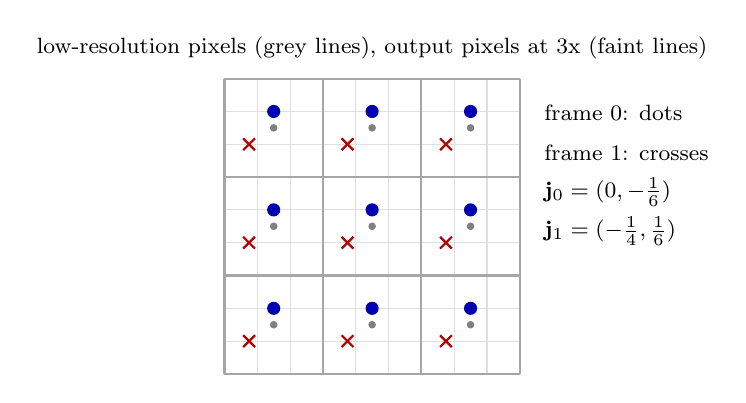
\begin{tikzpicture}[scale=1.25]
  \foreach \k in {0,...,9}{
    \draw[gray!25] (\k/3,-3) -- (\k/3,0);
    \draw[gray!25] (0,-\k/3) -- (3,-\k/3);
  }
  \draw[gray!70, thick] (0,-3) grid (3,0);
  \foreach \i in {0,1,2}{
    \foreach \j in {0,1,2}{
      \fill[gray] (\i+0.5,-\j-0.5) circle (1.1pt);
      \fill[blue!70!black] (\i+0.5,-\j-0.5+0.1667) circle (1.9pt);
      \draw[red!70!black, thick] (\i+0.25-0.06,-\j-0.6667-0.06) -- (\i+0.25+0.06,-\j-0.6667+0.06);
      \draw[red!70!black, thick] (\i+0.25-0.06,-\j-0.6667+0.06) -- (\i+0.25+0.06,-\j-0.6667-0.06);
    }
  }
  \node[anchor=south, font=\footnotesize] at (1.5,0.1) {low-resolution pixels (grey lines), output pixels at 3x (faint lines)};
  \node[anchor=west, font=\footnotesize] at (3.15,-0.35) {frame $0$: dots};
  \node[anchor=west, font=\footnotesize] at (3.15,-0.75) {frame $1$: crosses};
  \node[anchor=west, font=\footnotesize] at (3.15,-1.15) {$\mathbf j_0=(0,-\tfrac16)$};
  \node[anchor=west, font=\footnotesize] at (3.15,-1.55) {$\mathbf j_1=(-\tfrac14,\tfrac16)$};
\end{tikzpicture}
\caption{Sample positions of two consecutive frames inside a $3\times3$ patch of low-resolution pixels, with rows increasing downwards as in the code. Grey dots mark the pixel centres. Blue dots are the samples of frame $0$ and red crosses those of frame $1$, shifted by the first two Halton offsets of \cref{tab:bg-halton}. Faint lines mark the output pixels at 3x, which at this scale subdivide each low-resolution pixel into nine cells.}\label{fig:bg-jitter}
\end{figure}

\paragraph{Halton sequence.} The offsets come from the Halton $(2,3)$ sequence, a low-discrepancy sequence whose points spread evenly over the unit square with fewer large gaps than random points.\cite{halton1960efficiency} For an integer $n\ge1$ with base-$b$ digits $n=\sum_k d_k(n)\,b^k$, the radical inverse is
\begin{equation}
\varphi_b(n)=\sum_{k\ge0}d_k(n)\,b^{-(k+1)}.\label{eq:bg-halton}
\end{equation}
For example, $3=11_2$ gives $\varphi_2(3)=\tfrac12+\tfrac14=\tfrac34$, and $3=10_3$ gives $\varphi_3(3)=\tfrac19$. The function \texttt{halton} computes this by repeated division by the base. Frame $t$ uses the index $n_t=(t\bmod16)+1$ and the offset
\begin{equation}
\mathbf j_t=\big(\varphi_2(n_t)-\tfrac12,\ \varphi_3(n_t)-\tfrac12\big),\label{eq:bg-jitter}
\end{equation}
so the sequence repeats every 16 frames. The index starts at 1 because index 0 would give the corner $(-0.5,-0.5)$. Training gives each sample a random starting point in the cycle. \Cref{tab:bg-halton} lists the first four offsets, which \texttt{jitter\_sequence} produces.

\begin{table}[!htbp]
\caption{First four Halton jitter offsets. Frame $t$ uses index $n=(t\bmod16)+1$, and the offset $\mathbf j_t$ of Eq.~(\ref{eq:bg-jitter}) is in low-resolution pixels. The values were printed by \texttt{jitter\_sequence} and are rounded to three decimals}\label{tab:bg-halton}
\begin{tabular*}{\columnwidth}{@{\extracolsep\fill}rrrrrr}
\toprule
Frame $t$ & $n$ & $\varphi_2(n)$ & $\varphi_3(n)$ & $j_x$ & $j_y$ \\
\midrule
0 & 1 & $0.500$ & $0.333$ & $0.000$ & $-0.167$ \\
1 & 2 & $0.250$ & $0.667$ & $-0.250$ & $0.167$ \\
2 & 3 & $0.750$ & $0.111$ & $0.250$ & $-0.389$ \\
3 & 4 & $0.125$ & $0.444$ & $-0.375$ & $-0.056$ \\
\botrule
\end{tabular*}
\end{table}

\paragraph{Why jitter and accumulation recover resolution.} Take a static scene and one jittered sample per low-resolution pixel per frame. If the samples of earlier frames are placed at their true positions, using each frame's known offset, then after $N$ frames each low-resolution pixel holds $N$ samples at $N$ different positions. The output needs $s^2$ pixels per low-resolution pixel, so the samples must cover the $s^2$ sub-cells, and the Halton positions do this within a few frames. Jitter-aware upsampling does the placement: it samples the low-resolution frame at the output pixel centre minus the jitter (\texttt{jitter\_upsample}), so each sample lands at its true position.

Accumulation is a weighted average. Consider an exponential average $\hat y=\sum_{k\ge0}w_kx_{t-k}$ with weights $w_k=\alpha(1-\alpha)^k$, $0<\alpha\le1$, which sum to one. For samples $x_{t-k}$ with independent noise of variance $\sigma^2$,
\begin{equation}
\operatorname{Var}\hat y=\sum_{k\ge0}w_k^2\sigma^2=\frac{\alpha^2\sigma^2}{1-(1-\alpha)^2}=\frac{\alpha}{2-\alpha}\,\sigma^2,
\end{equation}
so the average behaves like a mean of $N_{\text{eff}}=(2-\alpha)/\alpha$ independent samples. For $\alpha=0.1$, the blend used by the analytic baseline of \cref{sec:bg-taa}, $N_{\text{eff}}=19$. This holds only when the history is aligned, so that a sample from an earlier frame belongs to the same surface point, and when the content is static. Motion and disocclusion break both conditions, which is why the next subsections need reprojection and rejection.

\subsection{Motion vectors and optical flow}\label{sec:bg-motion}

\paragraph{Flow.} For frames $t$ and $s$, the flow $F_{t\to s}$ is a field of displacements in pixels. For a pixel $\mathbf p$ of frame $t$, the point $\mathbf p+F_{t\to s}(\mathbf p)$ is the position in frame $s$ of the surface point that $\mathbf p$ shows in frame $t$. The code uses the backward convention for warping, in which the field is defined on the grid of the frame being produced, $t$, and points into the source frame $s$. Frame $t$ is then predicted from frame $s$ by
\begin{equation}
\hat I_t(\mathbf p)=I_s\big(\mathbf p+F_{t\to s}(\mathbf p)\big),\label{eq:bg-flow}
\end{equation}
which is the backward warp of \cref{sec:bg-warp}. A forward flow $F_{s\to t}$ is defined on the grid of the source frame and points forward. Datasets often store forward flow, and warping with it needs a scatter step that leaves holes and overlaps, so the code converts or reverses the flow instead. The code uses these conventions:
\begin{itemize}
\item Temporal super-resolution: the motion vector of frame $t$ is $m_t=F_{t\to t-1}$, the displacement from the current frame to the previous one, at low-resolution pixels (\texttt{sr\_batch}, \texttt{raft\_mv\_and\_valid}).
\item Frame generation: the engine motion vector of the newest real frame is $M_1=F_{1\to0}$, the displacement from $I_1$ to $I_0$ (\texttt{fg\_batch}).
\item Frame generation: the intermediate flows are $F_{\tau\to0}$ and $F_{\tau\to1}$, the outputs of \texttt{IFNet} (\cref{sec:bg-interp}).
\item Exact sources: the loader plays clips with forward flow backwards (\texttt{load\_clip}). The stored flow from frame $i$ to frame $i+1$ then becomes the displacement from the later frame to the earlier one, which is the convention of $m_t$, without any inversion.
\end{itemize}

\paragraph{Engine vectors and colour flow.} An engine writes a motion vector per pixel from the transforms of the geometry it draws. The vector is exact for opaque surfaces that the engine transforms, and particles and other effects without a transform get none, which is why engines also write a reactive mask. Research systems use such engine buffers, including motion vectors, as network inputs.\cite{xiao2020nsrr} Colour-only flow estimates motion from the images. It works on any video, but it is an estimate that can be wrong at boundaries, and it cannot separate motion from a change of lighting or from an overlay that moves independently. The code uses torchvision's RAFT-Small \cite{teed2020raft} with 12 updates (\texttt{load\_raft}, \texttt{raft\_flow}), as the teacher for motion labels on real video and for tOF. The built-in motion estimator of the temporal super-resolution network is an IFNet \cite{huang2022rife}.

\paragraph{Forward-backward consistency.} For two frames $a$ and $b$ with flows $F_{a\to b}$ and $F_{b\to a}$, a pixel passes the round-trip test when
\begin{equation}
\big\|F_{a\to b}(\mathbf p)+F_{b\to a}\big(\mathbf p+F_{a\to b}(\mathbf p)\big)\big\|<1+0.05\,\big\|F_{a\to b}(\mathbf p)\big\|,\label{eq:bg-fb}
\end{equation}
which says that going to frame $b$ and back returns to the start within one pixel plus 5 percent of the flow. The code's \texttt{raft\_mv\_and\_valid} applies this test with $a$ the current frame and marks the pixels that pass as valid. Pixels that fail lie at occlusions, at disocclusions and where the flow estimate is poor.

\paragraph{Occlusion and disocclusion.} A surface point is disoccluded in frame $t$ when it is visible in $t$ but absent from the previous frame $s$, and it is occluded when it is visible in $s$ but covered in $t$. The warp of Eq.~(\ref{eq:bg-flow}) has no correct source for a disoccluded pixel, so history must not be used there. The code's validity mask $v$ equals 1 where the pixel of frame $t$ is visible in the previous frame, so $1-v$ marks the disoccluded pixels (\texttt{load\_valid}). The temporal super-resolution network also uses a depth cue, $|d_t-\mathcal W(d_{t-1})|/(|d_t|+10^{-3})$, clipped to $[0,1]$, as an input feature (\texttt{TSRNet.forward}).

\paragraph{Scene cuts.} A cut is a change of content between consecutive frames. No point corresponds across it, so any flow is meaningless, and no frame can be predicted from the one before. The code detects cuts with the distance between normalised 32-bin histograms of the luma (\texttt{cut\_score}),
\begin{equation}
d_{\text{hist}}(I_0,I_1)=\tfrac12\sum_{b=1}^{32}\big|h_0(b)-h_1(b)\big|,\label{eq:bg-cut}
\end{equation}
where $h_0$ and $h_1$ are the normalised histograms of the two frames. This distance lies in $[0,1]$ and is the total-variation distance between the two histograms. When the motion vector $M_1$ is available, the score adds $2\,\overline{|I_1-\mathcal W(I_0,M_1)|}$, twice the mean motion-compensated difference. A score above a threshold is a cut.

\subsection{Warping, reprojection and history accumulation}\label{sec:bg-warp}

\paragraph{Backward warping.} Given a frame $I$ and a flow $F$, the warp $\mathcal W(I,F)(\mathbf p)=I(\mathbf p+F(\mathbf p))$ must be evaluated at non-integer positions. The code uses bilinear interpolation. For $\mathbf q=\mathbf p+F(\mathbf p)$ with integer part $(x_0,y_0)$ and fractional parts $a=q_x-x_0$ and $b=q_y-y_0$,
\begin{equation}\begin{split}
I(\mathbf q)&=(1-a)(1-b)\,I(x_0,y_0)+a(1-b)\,I(x_0+1,y_0)\\
&\quad+(1-a)b\,I(x_0,y_0+1)+ab\,I(x_0+1,y_0+1).
\end{split}\label{eq:bg-warp}\end{equation}
The four weights are non-negative and sum to one. Positions outside the frame are clamped to the border. Backward warping gathers each output pixel from one source location, so the output has no holes or overlaps, which forward splatting cannot guarantee. \texttt{backward\_warp} implements Eq.~(\ref{eq:bg-warp}) with \texttt{grid\_sample}, using the coordinate mapping of RIFE, in which pixel index $i$ corresponds to the normalised coordinate $-1+2i/(W-1)$. \Cref{fig:bg-warp} shows one pixel.

\begin{figure}[!htbp]
\centering
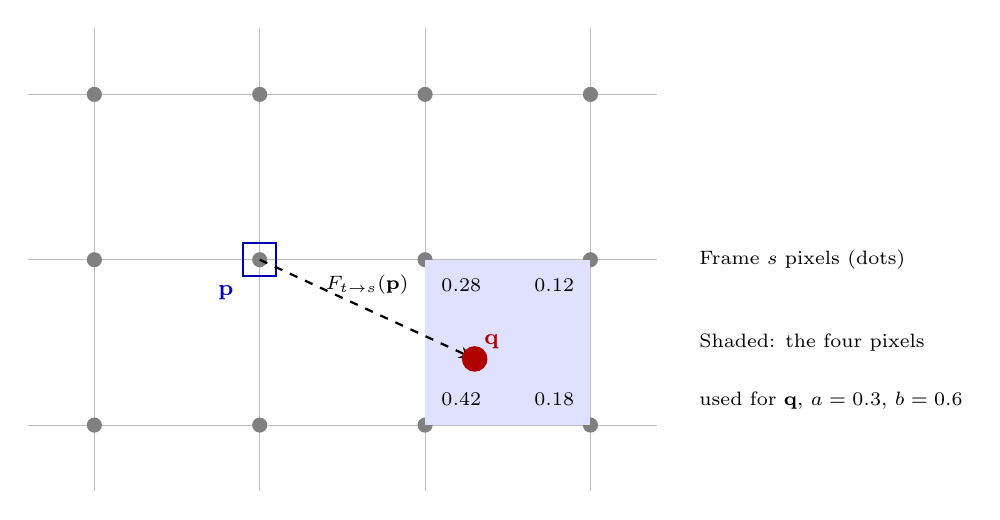
\begin{tikzpicture}[scale=2.1, font=\footnotesize]
  \draw[gray!50] (-0.4,-2.4) grid (3.4,0.4);
  \foreach \i in {0,...,3}{\foreach \j in {0,...,2}{\fill[gray] (\i,-\j) circle (1.3pt);}}
  \fill[blue!12] (2,-2) rectangle (3,-1);
  \draw[blue!70!black, thick] (0.9,-0.9) rectangle (1.1,-1.1);
  \node[anchor=north east, text=blue!70!black] at (0.9,-1.1) {$\mathbf p$};
  \draw[-{Stealth[length=2mm]}, thick, dashed] (1,-1) -- (2.3,-1.6);
  \node[anchor=south, font=\scriptsize] at (1.65,-1.27) {$F_{t\to s}(\mathbf p)$};
  \fill[red!70!black] (2.3,-1.6) circle (2.2pt);
  \node[anchor=south west, text=red!70!black] at (2.3,-1.6) {$\mathbf q$};
  \node[anchor=north west] at (2.04,-1.06) {\scriptsize $0.28$};
  \node[anchor=north east] at (2.96,-1.06) {\scriptsize $0.12$};
  \node[anchor=south west] at (2.04,-1.94) {\scriptsize $0.42$};
  \node[anchor=south east] at (2.96,-1.94) {\scriptsize $0.18$};
  \node[anchor=west] at (3.6,-1.0) {\scriptsize Frame $s$ pixels (dots)};
  \node[anchor=west] at (3.6,-1.5) {\scriptsize Shaded: the four pixels};
  \node[anchor=west] at (3.6,-1.85) {\scriptsize used for $\mathbf q$, $a=0.3$, $b=0.6$};
\end{tikzpicture}
\caption{Backward warp of one pixel. Pixel $\mathbf p=(1,1)$ of frame $t$ takes the value at $\mathbf q=\mathbf p+F_{t\to s}(\mathbf p)=(2.3,1.6)$ in frame $s$. That value is the bilinear mixture of the four surrounding pixels of frame $s$, with the weights shown from Eq.~(\ref{eq:bg-warp}). The flow is illustrative.}\label{fig:bg-warp}
\end{figure}

\paragraph{Half-pixel attenuation.} Bilinear interpolation is a low-pass filter. For a shift of half a pixel the weights are $(\tfrac12,\tfrac12)$, and the frequency response at angular frequency $\omega$ radians per pixel is $\tfrac12(1+e^{-i\omega})$, whose magnitude is $|\cos(\omega/2)|$. At $\omega=\pi/2$ this is $\cos(\pi/4)\approx0.71$, and at the Nyquist frequency $\omega=\pi$ it is zero. Each warp at a fractional offset removes part of the high-frequency content. A recurrent network that warps its output every frame loses high frequencies at every step unless its residual path adds them back.

\paragraph{Reprojection and accumulation.} Reprojection moves a stored result to the current frame. A history image $H$ from frame $t-1$ becomes $H_t(\mathbf p)=\mathcal W(H,m_t)(\mathbf p)$ with $m_t=F_{t\to t-1}$, and accumulation then combines $H_t$ with the new samples. The recurrent state of the temporal super-resolution network, its output and its hidden feature map, is reprojected in the same way with the low-resolution vectors. A pixel whose motion is wrong, or which is disoccluded, takes its history from the wrong surface, and that is the source of the ghosting described in \cref{sec:bg-taa}.

\subsection{Temporal anti-aliasing and temporal upscaling}\label{sec:bg-taa}

Temporal anti-aliasing (TAA) \cite{yang2020taasurvey} combines jittered samples over time with a history buffer. For each frame it renders with a jittered sample grid, reprojects the history with motion vectors, clamps the reprojected history to the range of the current samples in a small neighbourhood, and blends the clamped history with the current samples. Temporal upscaling runs the same loop at a lower render resolution, with the accumulation buffer at output resolution.

\paragraph{Exponential blending.} Without reprojection and clamping, accumulation is $\hat y_t=\alpha x_t+(1-\alpha)\hat y_{t-1}$, where $x_t$ is the current sample value and $0<\alpha\le1$. Unrolling gives
\begin{equation}
\hat y_t=\sum_{k=0}^{t-1}\alpha(1-\alpha)^k\,x_{t-k}+(1-\alpha)^t\,\hat y_0,\label{eq:bg-ema-unroll}
\end{equation}
so the sample $k$ frames old has weight $\alpha(1-\alpha)^k$, and the initial value keeps the weight $(1-\alpha)^t$. \Cref{fig:bg-ema} shows these weights for $\alpha=0.1$. A sample 10 frames old has weight $0.035$, and the initial value still has weight $0.12$ after 20 frames.

\begin{figure}[!htbp]
\centering
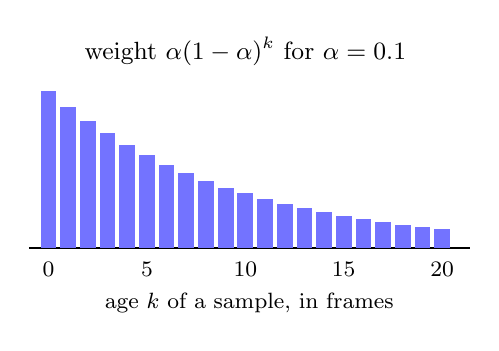
\begin{tikzpicture}[x=0.5cm, font=\footnotesize]
  \draw[thick] (-0.3,0) -- (10.9,0);
  \foreach \k/\h in {0/2.00,1/1.80,2/1.62,3/1.46,4/1.31,5/1.18,6/1.06,7/0.96,8/0.86,9/0.77,10/0.70,11/0.63,12/0.56,13/0.51,14/0.46,15/0.41,16/0.37,17/0.33,18/0.30,19/0.27,20/0.24}{
    \fill[blue!55] (\k*0.5,0) rectangle (\k*0.5+0.4,\h);
  }
  \foreach \k in {0,5,10,15,20}{
    \node[below] at (\k*0.5+0.2,-0.05) {\k};
  }
  \node[below] at (5.3,-0.45) {age $k$ of a sample, in frames};
  \node[above] at (5.2,2.2) {\small weight $\alpha(1-\alpha)^k$ for $\alpha=0.1$};
\end{tikzpicture}
\caption{Weight of a sample $k$ frames old in the exponential average of \cref{eq:bg-ema-unroll} with $\alpha=0.1$. The bar height is the weight times 20, in centimetres of the drawing. The weights fall geometrically, so an old surface that stays in the history fades slowly, which is the ghosting trail that clamping limits.}\label{fig:bg-ema}
\end{figure}

\paragraph{Ghosting.} When a surface changes, because it is disoccluded, because its motion vector is wrong or because an object leaves a region, the history still holds the old surface. That surface keeps the weight $(1-\alpha)^k$ for $k$ frames and appears as a trail behind moving objects. Clamping limits the trail. The reprojected value is confined to the range of the current neighbourhood, so an old colour far from the new samples is pulled back to the range boundary. Ghosting remains when the old colour lies inside that range, which happens when a surface and its background have similar colours. A larger $\alpha$ reduces ghosting but also reduces the averaging that removes aliasing, and that trade-off is the central design choice of TAA.

\paragraph{Analytic baseline.} The analytic upscaler of the evaluation (\texttt{AnalyticTAAU} in \texttt{nss\_metrics.py}, run by \texttt{run\_taau} in \texttt{nss\_eval.py}) implements the loop with fixed rules and stands in for analytic TAA upscalers without their proprietary heuristics. For frame $t$, with low-resolution colour $x_t$, jitter $\mathbf j_t$ and low-resolution motion vector $m_t$, it performs the following steps.
\begin{enumerate}
\item Base image: $B_t(\mathbf p)$ is the bilinear interpolation of $x_t$ at the low-resolution position of the output pixel centre $\mathbf p$ minus $\mathbf j_t$, so each sample is placed at its true position.
\item If there is no history, the output is $B_t$.
\item History: $H_t=\mathcal W\big(\hat y_{t-1},\,s\,U(m_t)\big)$, where $U$ is bilinear upsampling by $s$ and the factor $s$ converts low-resolution displacements into output pixels.
\item Clamp: with $lo$ and $hi$ the channel-wise minimum and maximum of YCoCg$(B_t)$ over the $3\times3$ output neighbourhood of each pixel, the history is clamped in YCoCg to the box between $lo$ and $hi$, and $H'_t$ is the RGB value of the clamped history.
\item Blend: $\hat y_t=H'_t+0.1\,(B_t-H'_t)$, which is 90 percent history and 10 percent current base image.
\end{enumerate}
The displayed output is clamped to $[0,1]$, but the unclamped value becomes the next history. Step 5 gives
\begin{equation}
\hat y_t=0.9\,H'_t+0.1\,B_t.\label{eq:bg-taa}
\end{equation}

Two properties of this baseline matter for the comparison. First, its docstring says that it resets on invalid history, but the code has no validity test, so every frame reprojects and clamps the history and no disocclusion rejection takes place. Second, the motion vectors are sampled at the jittered sample positions (\texttt{\_sr\_inputs}), while the baseline interprets low-resolution vectors as if they were at the pixel centres. The resulting error is the jitter times the local gradient of the motion field, which vanishes for uniform motion and is largest at motion boundaries. The temporal super-resolution network receives the same low-resolution vectors and interprets them in the same way. The supplement describes these properties as they are in the code.

\subsection{Neural building blocks}\label{sec:bg-cnn}

The networks use a small set of operators. Each is defined here with the code's convention and with the reason for its use.

\paragraph{Convolution and multiply-accumulates.} A convolutional layer with $C_{\text{in}}$ input channels, $C_{\text{out}}$ output channels and a $k\times k$ kernel $K$ computes, with stride 1 and padding $(k-1)/2$,
\begin{equation}
Y[o,i,j]=b_o+\sum_{c=1}^{C_{\text{in}}}\sum_{u=0}^{k-1}\sum_{v=0}^{k-1}K[o,c,u,v]\;X\!\Big[c,\;i+u-\tfrac{k-1}{2},\;j+v-\tfrac{k-1}{2}\Big],\label{eq:bg-conv}
\end{equation}
where $X$ is the input, $Y$ the output and $b_o$ the bias of output channel $o$. The sum is a cross-correlation, which is PyTorch's convention. One multiply-accumulate (MAC) is one multiplication followed by one addition. Each output element of Eq.~(\ref{eq:bg-conv}) costs $C_{\text{in}}k^2$ MACs, so a layer with an $H\times W$ output costs
\begin{equation}
M=H\,W\,C_{\text{out}}\,C_{\text{in}}\,k^2\qquad\text{MACs},\label{eq:bg-macs}
\end{equation}
and grouped convolutions divide this by the number of groups. A transposed convolution from an $H_{\text{in}}\times W_{\text{in}}$ input costs $H_{\text{in}}W_{\text{in}}C_{\text{in}}C_{\text{out}}k^2$, because each input pixel scatters a $k\times k$ kernel into every output channel. Pixel shuffles, bilinear resizing and grid sampling perform no such multiply-accumulates in the count, so the warps are excluded from the cost figures, as in \cref{M-tab:tiers}. For example, a $3\times3$ convolution with 24 input and 24 output channels costs $24\cdot24\cdot9=5{,}184$ MACs per output pixel.

\paragraph{Cost per 1080p frame.} The code counts MACs with forward hooks (\texttt{count\_macs}) on the fused network, which is the deployed form in which every block is a plain convolution. For temporal super-resolution it runs one step with a history state on a $64\times64$ low-resolution input, including the built-in motion estimator, and divides the count by $64^2$ to obtain MACs per low-resolution pixel (\texttt{tsr\_macs\_per\_lr\_pixel}). Each layer's cost is proportional to its pixel count, so the cost of one output frame is that per-pixel count times the number of low-resolution pixels of the 1080p output,
\begin{equation}
G_{1080p}=\frac{M_{\text{pix}}\,(1920/s)(1080/s)}{10^{9}}\quad\text{GMAC}.\label{eq:bg-gmac}
\end{equation}
For frame generation the fused network runs on a $272\times480$ frame. The flow-resolution limit is scaled by $272/1080$ so that the flow runs at the scale that a 1080p frame would use, the MACs are counted, and the count is multiplied by $(1920\cdot1080)/(272\cdot480)$. This assumes that the cost is linear in the pixel count, which holds for convolutions and is approximate for the remaining operators. A MAC count is a cost measure and not a time, and the latency measurements are reported separately.

\paragraph{Pixel shuffle.} Pixel shuffle \cite{shi2016espcn} rearranges a tensor with $C r^2$ channels at $H\times W$ into $C$ channels at $rH\times rW$,
\begin{equation}
Z[c,\;rh+a,\;rw+b]=X[c\,r^2+a\,r+b,\;h,\;w],\qquad 0\le a,b<r,\label{eq:bg-shuffle}
\end{equation}
without any multiplication. Its inverse, pixel unshuffle or space-to-depth, folds a tensor at $rH\times rW$ into $r^2$ times as many channels at $H\times W$. A convolution can therefore run at low resolution, where it is cheap, and the shuffle restores the output size. The temporal super-resolution network uses both directions. Its output convolution produces $4s^2$ channels at low resolution, which the shuffle turns into a residual and a history weight at output resolution, and it folds the reprojected output into $3s^2$ low-resolution channels before the trunk reads it.

\paragraph{Structural re-parameterisation.} A block can be trained as several parallel linear branches and deployed as one convolution. This works when the branches share their input and their spatial support, because convolution is linear in its kernel. The RepConv block of \texttt{nss\_models.py} has four branches on the same input $x$, with $C_{\text{in}}$ input and $C_{\text{out}}$ output channels:
\begin{enumerate}
\item a $3\times3$ convolution with kernel $W_3$ and bias $b_3$.
\item a $1\times1$ convolution with kernel $W_1$ and bias $b_1$.
\item the identity, present when $C_{\text{in}}=C_{\text{out}}$.
\item fixed edge filters $E_1$ (Sobel $x$), $E_2$ (Sobel $y$) and $E_3$ (Laplacian), applied to every input channel, whose $3C_{\text{in}}$ responses are combined by a learned $1\times1$ projection $P\in\mathbb R^{C_{\text{out}}\times3C_{\text{in}}}$ with bias $b_e$.
\end{enumerate}
The block output is $\phi(Y)$, where $\phi$ is a PReLU activation and $Y$ is the sum of the four branch outputs.

The four branches fold into one $3\times3$ convolution, exactly:
\begin{equation}\begin{split}
Y&=\sum_{c}K[\cdot,c]\ast x_c+b,\\
K[o,c]&=W_3[o,c]+\operatorname{pad}\big(W_1[o,c]\big)\\
&\quad+\sum_{k=1}^{3}\tilde P[o,c,k]\,E_k+\delta_{oc}\,\Delta,\\
b&=b_3+b_1+b_e,
\end{split}\label{eq:bg-fold}\end{equation}
where $\ast$ is convolution with stride 1 and padding 1, $\operatorname{pad}$ places a scalar at the centre tap of an otherwise zero $3\times3$ kernel, $\tilde P[o,c,k]=P[o,\,3c+k]$ reorders the projection by input channel, $\delta_{oc}$ is the Kronecker delta and $\Delta$ is the $3\times3$ kernel with 1 at its centre and 0 elsewhere.

\emph{Proof.} Each branch is linear in $x$ and is a convolution with stride 1 and padding 1, so each can be written as a $3\times3$ convolution. (1) The $1\times1$ branch outputs $W_1[o,c]\,x_c(\mathbf p)$. With padding 1, a $3\times3$ kernel whose only nonzero tap is the centre, with value $W_1[o,c]$, produces the same output, and that kernel is $\operatorname{pad}(W_1[o,c])$. (2) The identity outputs $x_o(\mathbf p)$, which is the kernel $\Delta$ on the diagonal $c=o$. (3) The edge branch outputs $\sum_c\sum_k P[o,3c+k]\,(E_k\ast x_c)(\mathbf p)+b_e[o]$. Convolution is linear in its kernel, so $\sum_k\tilde P[o,c,k]\,(E_k\ast x_c)=\big(\sum_k\tilde P[o,c,k]E_k\big)\ast x_c$, and the branch is a $3\times3$ convolution with kernel $\sum_k\tilde P[o,c,k]E_k$ and bias $b_e[o]$. (4) For a common stride and padding, $(A\ast x)+(B\ast x)=(A+B)\ast x$, so the four branch sums combine into Eq.~(\ref{eq:bg-fold}). The activation is applied after the sum, so it is not folded, and the fold is exact. Up to floating-point rounding, the fused and unfused outputs are identical, and the code's fusion-parity test checks this numerically. $\square$

Training uses the folded kernel directly. The code recomputes $K$ from the branch parameters on every forward pass (online re-parameterisation), so a block costs one $3\times3$ convolution during training as well as in deployment. The function class is unchanged, because $W_3$ alone can represent any kernel that the block can reach. The extra branches only change which kernels gradient descent reaches. The $1\times1$ and edge-projection weights start at zero, so the block starts as a $3\times3$ convolution plus the identity. Only the weights are zeroed, so the small biases $b_1$ and $b_e$ remain at their random initial values. \Cref{fig:bg-fold} summarises the fold.

\begin{figure}[!htbp]
\centering
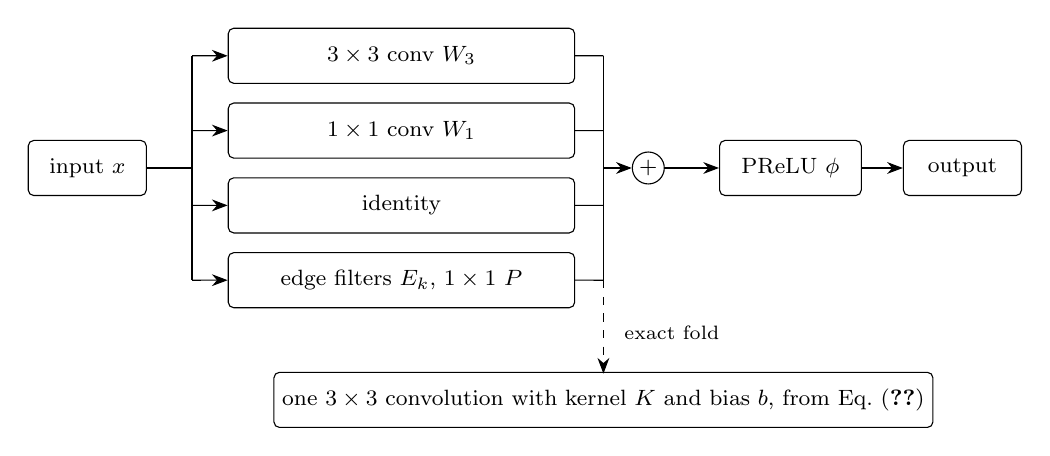
\begin{tikzpicture}[scale=0.95, font=\footnotesize, node distance=3mm,
  box/.style={draw, rounded corners=2pt, align=center, minimum height=7mm, minimum width=4.4cm, inner sep=3pt},
  arr/.style={-{Stealth[length=2mm]}}]
\node[box, minimum width=1.5cm] (x) at (0,0) {input $x$};
\node[box] (w3) at (4.2,1.5) {$3\times3$ conv $W_3$};
\node[box] (w1) at (4.2,0.5) {$1\times1$ conv $W_1$};
\node[box] (id) at (4.2,-0.5) {identity};
\node[box] (ed) at (4.2,-1.5) {edge filters $E_k$, $1\times1$ $P$};
\node[draw, circle, inner sep=1pt] (sum) at (7.5,0) {$+$};
\node[box, minimum width=1.8cm] (act) at (9.4,0) {PReLU $\phi$};
\node[box, minimum width=1.5cm] (out) at (11.7,0) {output};
\draw (x.east) -- (1.4,0);
\draw (1.4,1.5) -- (1.4,-1.5);
\draw[arr] (1.4,1.5) -- (w3.west);
\draw[arr] (1.4,0.5) -- (w1.west);
\draw[arr] (1.4,-0.5) -- (id.west);
\draw[arr] (1.4,-1.5) -- (ed.west);
\draw (w3.east) -- (6.9,1.5);
\draw (w1.east) -- (6.9,0.5);
\draw (id.east) -- (6.9,-0.5);
\draw (ed.east) -- (6.9,-1.5);
\draw (6.9,1.5) -- (6.9,-1.5);
\draw[arr] (6.9,0) -- (sum.west);
\draw[arr] (sum.east) -- (act.west);
\draw[arr] (act.east) -- (out.west);
\node[box, minimum width=7.0cm] (k) at (6.9,-3.1) {one $3\times3$ convolution with kernel $K$ and bias $b$, from Eq.~(\ref{eq:bg-fold})};
\draw[arr, dashed] (6.9,-1.5) -- (6.9,-2.75);
\node[anchor=west, font=\scriptsize] at (7.05,-2.2) {exact fold};
\end{tikzpicture}
\caption{Re-parameterisation of one RepConv block. The four linear branches share the input and sum before the activation, giving one kernel $K$ and bias $b$ of size $3\times3$.}\label{fig:bg-fold}
\end{figure}

\paragraph{U-Net levels.} The trunk of the temporal super-resolution network has an optional half-resolution level. It differs from the classic U-Net,\cite{ronneberger2015unet} so it is described precisely here. A strided $3\times3$ convolution halves the resolution and doubles the channels. Residual blocks run at half resolution, a $1\times1$ convolution doubles the channels to $4w$, and a pixel shuffle returns to full resolution with $w$ channels. The result is added to the features that entered the level, which is an additive skip, where the classic U-Net concatenates. A convolution with $2w$ channels at half resolution costs the same as one with $w$ channels at full resolution, because $(2w)^2\cdot\tfrac14=w^2$, but each of its taps covers twice the distance in the original image.

\paragraph{Recurrent networks and hidden-state warping.} A recurrent network carries a state from frame to frame. The state of the temporal super-resolution network holds the previous output $\hat y_{t-1}$, a hidden feature map $h_{t-1}$, and the previous depth, colour and jitter. At each frame the network reads the current inputs together with the reprojected output and hidden state, and writes the new output and a new hidden state $h_t=\tanh(\cdot)$ of a convolution. The hidden state is reprojected with the same motion as the output, $\mathcal W(h_{t-1},m_t)$, because its channels describe the content at each pixel, and a feature warped with the wrong motion describes a different surface. Training unrolls the network over several frames, with a 16-frame unroll every fourth step, and backpropagates through the whole unroll, which is backpropagation through time. During the first quarter of training (\texttt{mv\_warmup\_frac} $=0.25$), samples without motion vectors warp the history with the label motion instead of the estimated motion. The probability of doing so falls linearly from one to zero over that quarter. Feeding the label in place of the model's own estimate is teacher forcing, which this code applies as a schedule, and the schedule stops the history path from learning to ignore history while the estimator is still poor.

\paragraph{Zero initialisation.} A branch whose output layer has zero weights and a zero bias contributes exactly zero at initialisation, so the network starts as the network without that branch. Two consequences follow. The output layer receives a nonzero gradient, because its input features are nonzero, so it learns from the first step. The layers upstream of it receive a zero gradient at the first step, because they reach the loss only through the zero weights, and they start to learn once the output layer is nonzero. The bias must also be zero, because a nonzero bias gives a constant contribution at initialisation. The code uses three instances.
\begin{itemize}
\item The engine-hint input channels of the first convolution in each IFNet block have zero weights, so the hints do not change that layer's output at initialisation. This is exact.
\item The frame generator's residual head has zero weights and a zero bias, so its colour residual $r$ is zero at initialisation. Its UI logit has a bias of $-4$, so the UI weight is $u=\sigma(-4)\approx0.018$ at initialisation. The output is therefore $u\,I_1+(1-u)$ times the RIFE blend $m\mathcal W(I_0,F_{\tau\to0})+(1-m)\mathcal W(I_1,F_{\tau\to1})$, and differs from that blend by $u\,(I_1-\text{blend})$. The code's parity test compares the blend, not the final output, so a fresh model reproduces the blend of RIFE exactly and not its final output.
\item The temporal super-resolution output layer has zero weights and a zero bias, so the residual is zero and the history weight is $\sigma(0+2)\approx0.88$, since the code adds 2 to the logit before the sigmoid. At initialisation the output is therefore $0.88$ of the history and $0.12$ of the jitter-aware upsampling, an exponential blend of the kind described in \cref{sec:bg-taa}.
\end{itemize}

\paragraph{Mixed precision and loss scaling.} In IEEE half precision (FP16) a value has one sign bit, five exponent bits and ten fraction bits. Its largest finite value is $(2-2^{-10})\,2^{15}=65{,}504$, its smallest positive normal value is $2^{-14}\approx6.1\cdot10^{-5}$, and its smallest positive subnormal value is $2^{-24}\approx6.0\cdot10^{-8}$. Two failures follow. Activations above 65{,}504 become infinite, and gradients much smaller than $6\cdot10^{-8}$ round to zero. Mixed precision \cite{micikevicius2018mixed} runs the forward and backward passes in FP16 and keeps FP32 copies of the weights. Loss scaling multiplies the loss by a scale $S$ before the backward pass, so that small gradients stay representable, and divides the gradients by $S$ before the optimiser step. Dynamic loss scaling lowers $S$ when a step produces non-finite gradients and raises it again after a run of finite steps. The code uses PyTorch's \texttt{GradScaler} with autocast. It scales the loss, unscales the gradients, clips their norm to 1.0 (\texttt{grad\_clip}) and then steps the optimiser. A run stops when the loss stays non-finite for 200 steps by default.

\paragraph{Exponential moving average.} The optimiser updates the weights $w_k$, and the code also keeps the average
\begin{equation}
\bar w_k=d_k\,\bar w_{k-1}+(1-d_k)\,w_k,\qquad d_k=\min\!\Big(0.999,\ \frac{1+k}{10+k}\Big),\label{eq:bg-ema}
\end{equation}
which is used for validation and checkpoints, while the raw weights produce the gradients. The warm-up in $d_k$ means that the decay reaches 0.999 only after about 9{,}000 steps, so early in training the average follows the weights closely. At a decay of 0.999 the average has a memory of about $1/(1-0.999)=1{,}000$ steps.

\paragraph{AdamW.} AdamW \cite{loshchilov2019adamw} keeps running averages of the gradient and of its square, $m_k=\beta_1 m_{k-1}+(1-\beta_1)g_k$ and $v_k=\beta_2 v_{k-1}+(1-\beta_2)g_k^2$, corrects their start-up bias and applies
\begin{equation}
\theta_k=\theta_{k-1}-\eta\Big(\frac{\hat m_k}{\sqrt{\hat v_k}+\epsilon}+\lambda\,\theta_{k-1}\Big),\qquad \hat m_k=\frac{m_k}{1-\beta_1^k},\quad \hat v_k=\frac{v_k}{1-\beta_2^k},\label{eq:bg-adamw}
\end{equation}
where $g_k$ is the gradient, $\eta$ the learning rate and $\lambda$ the weight decay. The decay term $\lambda\theta$ acts on the weights directly and is not added to the gradient, which is the difference from Adam with an L2 penalty. The code uses $(\beta_1,\beta_2)=(0.9,0.99)$, PyTorch's default $\epsilon=10^{-8}$ and $\lambda=10^{-4}$.

\paragraph{Learning-rate schedule.} The schedule is driven by wall-clock time rather than by the step count. With progress $p\in[0,1]$, the elapsed fraction of the run's time budget, a warm-up fraction $w=0.03$, a peak rate $\eta_0$ and a floor $\eta_{\min}=10^{-6}$,
\begin{equation}
\eta(p)=\begin{cases}\eta_0\,\max(p/w,\,0.01), & p<w,\\[2pt] \eta_{\min}+\tfrac12(\eta_0-\eta_{\min})\big(1+\cos\pi\tau\big), & \tau=\dfrac{p-w}{1-w}\ge0,\end{cases}\label{eq:bg-cosine}
\end{equation}
which is \texttt{lr\_at}. The learning rate follows a single cosine decay without restarts, the decay used within each cycle of SGDR \cite{loshchilov2017sgdr}. The peak rates are $2\cdot10^{-3}$ for the temporal super-resolution student, $10^{-3}$ for its teacher, $4\cdot10^{-4}$ for the frame-generation students and $10^{-4}$ for the frame-generation tier fine-tuned from RIFE 4.26. Because the schedule follows wall-clock time, a slower GPU performs fewer updates in the same budget.

\paragraph{Charbonnier loss.} The Charbonnier penalty \cite{charbonnier1997deterministic} is a smooth edge-preserving potential that approximates the absolute error,
\begin{equation}
\rho_\epsilon(e)=\sqrt{e^2+\epsilon^2},\qquad \epsilon=10^{-3},\label{eq:bg-charb}
\end{equation}
which is differentiable at zero and tends to $|e|$ for large errors. Its gradient $e/\rho_\epsilon(e)$ has magnitude at most one, so large errors do not dominate the gradient as they do under a squared error. The code averages $\rho_\epsilon$ over the elements (\texttt{charbonnier}), with an optional mask that normalises by the number of masked elements.

\subsection{Video frame interpolation and extrapolation}\label{sec:bg-interp}

Given real frames $I_0$ at time 0 and $I_1$ at time 1, interpolation produces $I_\tau$ for $0<\tau<1$. Extrapolation produces $I_\tau$ for $\tau>1$ from frames at or before time 1 only. \Cref{fig:bg-tau} shows the time axis of both modes. Multi-frame generation with a factor $N$ inserts $N-1$ frames between real frames, so 3x generation uses $\tau=\tfrac13$ and $\tau=\tfrac23$. Generation raises the displayed frame rate without rendering the scene again, but it has to wait for the real frame it needs, as \cref{sec:bg-latency} explains.

\begin{figure}[!htbp]
\centering
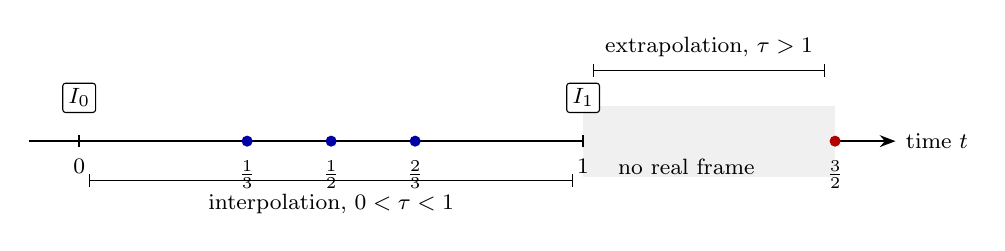
\begin{tikzpicture}[x=6.4cm, font=\footnotesize]
  \draw[thick, -{Stealth[length=2mm]}] (-0.1,0) -- (1.62,0) node[right] {time $t$};
  \fill[gray!12] (1,-0.45) rectangle (1.5,0.45);
  \draw[thick] (0,-0.08) -- (0,0.08);
  \draw[thick] (1,-0.08) -- (1,0.08);
  \node[draw, rounded corners=1pt, fill=white, inner sep=2pt] at (0,0.55) {$I_0$};
  \node[draw, rounded corners=1pt, fill=white, inner sep=2pt] at (1,0.55) {$I_1$};
  \node[below] at (0,-0.1) {$0$};
  \node[below] at (1,-0.1) {$1$};
  \foreach \x/\lab in {0.3333/{$\tfrac13$}, 0.5/{$\tfrac12$}, 0.6667/{$\tfrac23$}}{
    \fill[blue!65!black] (\x,0) circle (2pt);
    \node[below] at (\x,-0.12) {\lab};
  }
  \fill[red!70!black] (1.5,0) circle (2pt);
  \node[below] at (1.5,-0.12) {$\tfrac32$};
  \draw[|-|] (0.02,-0.5) -- (0.98,-0.5);
  \node[below] at (0.5,-0.55) {\footnotesize interpolation, $0<\tau<1$};
  \draw[|-|] (1.02,0.9) -- (1.48,0.9);
  \node[above] at (1.25,0.95) {\footnotesize extrapolation, $\tau>1$};
  \node[anchor=west, font=\footnotesize] at (1.05,-0.32) {no real frame};
\end{tikzpicture}
\caption{Time axis of the two generation modes with real frames $I_0$ and $I_1$. Interpolation (blue) places generated frames between the real frames, at $\tau=\tfrac12$ or at the two positions of 3x generation. Extrapolation (red) places a generated frame after $I_1$ at $\tau=\tfrac32$ using only frames at or before time 1. The shaded interval has no real frame.}\label{fig:bg-tau}
\end{figure}

\paragraph{Intermediate flows.} The generator needs the motion from each real frame to the intermediate time $\tau$, which is $F_{\tau\to0}$ and $F_{\tau\to1}$ as defined in \cref{sec:bg-motion}. Under constant velocity, a surface point moves as $\mathbf p(\tau)=\mathbf p_0+\tau\mathbf v$, where $\mathbf v$ is its displacement from time 0 to time 1, so that $\mathbf p_1=\mathbf p_0+\mathbf v$. Its displacement from $I_1$ to $I_0$ is $M_1=-\mathbf v$, and therefore
\begin{equation}
F_{\tau\to0}=\tau M_1,\qquad F_{\tau\to1}=(\tau-1)M_1,\label{eq:bg-linear}
\end{equation}
which are the linear-motion priors of the frame generator. To see this, note $F_{\tau\to0}=\mathbf p_0-\mathbf p(\tau)=-\tau\mathbf v=\tau M_1$, and $F_{\tau\to1}=\mathbf p_1-\mathbf p(\tau)=(1-\tau)\mathbf v=(\tau-1)M_1$. The code evaluates $M_1$ at the target pixel rather than at the moving point, which is exact when the motion field is locally constant.

\paragraph{Coarse-to-fine estimation.} The intermediate flows come from an IFNet with the design of RIFE 4.26 \cite{huang2022rife}. It is a chain of blocks, each working at a fraction $1/s_k$ of the input resolution, with scales $16,8,4,2,1$ for the five blocks of the full network. Each block predicts a blend logit and an update to the flow at its own resolution. The update is resampled to full resolution and multiplied by $s_k$, because a displacement in pixels scales with resolution, so
\begin{equation}
F^{(k)}=F^{(k-1)}+s_k\,\mathcal U_{s_k}\big(\tilde\Delta^{(k)}\big),\label{eq:bg-c2f}
\end{equation}
where $\tilde\Delta^{(k)}$ is the raw update of block $k$ and $\mathcal U_{s_k}$ is bilinear upsampling by $s_k$. The coarse blocks capture large motion at low cost, and the fine blocks add detail.

\paragraph{Blending.} The two warped frames are combined with a per-pixel blend $m\in[0,1]$, which is the sigmoid of the network's logit,
\begin{equation}
\hat I_\tau=m\odot\mathcal W(I_0,F_{\tau\to0})+(1-m)\odot\mathcal W(I_1,F_{\tau\to1}),\label{eq:bg-blend}
\end{equation}
where $\odot$ is the element-wise product. Where a surface is visible in only one real frame, the correct blend selects that frame, and this is how interpolation handles occlusions.

\paragraph{Resolution rule and cuts.} Flow is costly, so the generator estimates it at a reduced scale for tall frames. The flow scale is the largest $2^{-k}$ with $H\,2^{-k}\le L$, where $L$ is the flow limit of the tier, 576 or 1152 lines. At 1080p this gives 540 lines for $L=576$ and full resolution for $L=1152$. When two real frames come from different scenes, the flows and the blend describe no correspondence, so generation should not run. The code repeats $I_1$ in that case, as \cref{sec:bg-motion} describes. Interpolation also fails where the motion exceeds what the flow search can resolve, at disocclusions where the blend cannot choose, for particles and other motion without correspondence, and on overlays such as text and HUD elements that move differently from the scene.

\subsection{Frame budgets, pacing and latency}\label{sec:bg-latency}

\paragraph{Frame budget.} A display that refreshes $R$ times per second shows a new frame every $1000/R$ milliseconds. That is 16.7 ms at 60 Hz, 33.3 ms at 30 Hz and 8.3 ms at 120 Hz. A renderer that cannot finish a frame within the interval either presents it late or repeats the previous one, so every stage of the frame must fit the budget if the rate is to be sustained. The stages are a CPU update of $c$ ms, a GPU render of $r$ ms, the upscaling of $s$ ms, the frame generation of $g$ ms and the presentation of $p$ ms. In a GPU-bound loop the period is set by the GPU, so the period of a generating loop is $P=\max(c,\,r+s+g)$, the rule that \texttt{simulate\_latency} applies, and the CPU work starts just in time so that no frame waits in a queue.

\paragraph{Three quantities that differ.} Three measures are easily confused.
\begin{itemize}
\item The rendered frame rate is the number of real frames per second that the engine produces, which is $1000/P$ for a loop without generation.
\item The displayed frame rate is the number of frames presented per second, including generated frames. With one generated frame per real frame it is about twice the rendered rate, provided that generation does not lengthen the period, and in a GPU-bound loop it does lengthen it.
\item The input latency is the time from an input sample to the first photons of a frame that reflects it. The frame rate does not determine it.
\end{itemize}

\paragraph{Latency of interpolation and extrapolation.} Interpolation shows a generated frame between $I_{k-1}$ and $I_k$, which needs $I_k$ to exist. The real frame $I_k$ is therefore held until the generated frame has been shown, and it is shown about half a period later, so the input latency of a real frame rises by $g+P/2$. Extrapolation generates from past frames only, so a real frame is presented as soon as it is rendered and its latency does not change. The generated frame follows the real frame, and in the simulator it is presented half a period after it. \Cref{fig:bg-pacing} shows the presentation times that these rules give for one real frame in each mode.

\begin{figure}[!htbp]
\centering
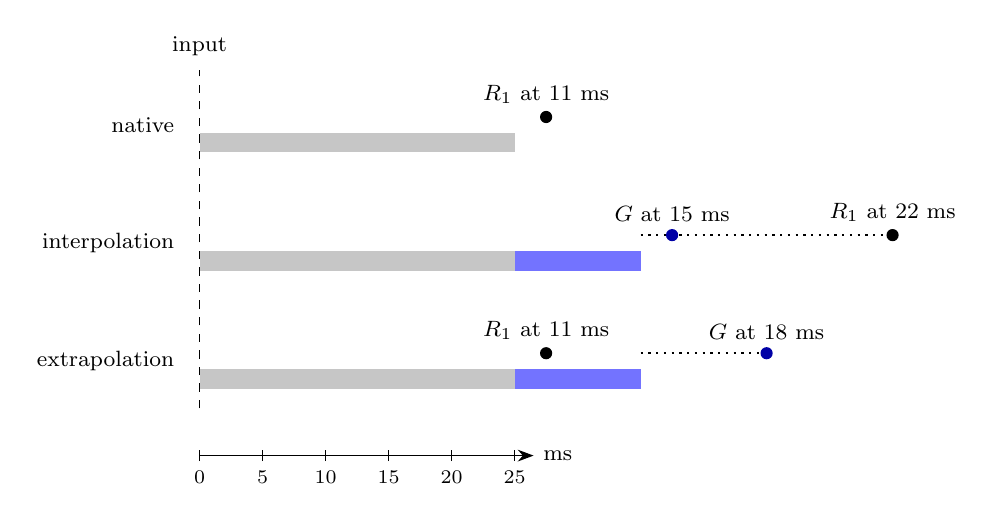
\begin{tikzpicture}[x=0.4cm, y=1cm, font=\footnotesize]
  \node[anchor=east] at (-0.5,3) {native};
  \node[anchor=east] at (-0.5,1.5) {interpolation};
  \node[anchor=east] at (-0.5,0) {extrapolation};
  \draw[dashed] (0,-0.6) -- (0,3.7);
  \node[anchor=south] at (0,3.75) {input};
  % native: render 0 to 10 ms, real frame shown at 11 ms
  \fill[gray!45] (0,2.65) rectangle (10,2.9);
  \fill[black] (11,3.1) circle (2.2pt);
  \node[anchor=south] at (11,3.15) {$R_1$ at 11 ms};
  % interpolation: render 0 to 10, generate 10 to 14, G shown at 15, R1 held and shown at 22
  \fill[gray!45] (0,1.15) rectangle (10,1.4);
  \fill[blue!55] (10,1.15) rectangle (14,1.4);
  \draw[dotted, thick] (14,1.6) -- (22,1.6);
  \fill[blue!65!black] (15,1.6) circle (2.2pt);
  \node[anchor=south] at (15,1.65) {$G$ at 15 ms};
  \fill[black] (22,1.6) circle (2.2pt);
  \node[anchor=south] at (22,1.65) {$R_1$ at 22 ms};
  % extrapolation: render 0 to 10, generate 10 to 14, R1 shown at 11, G shown at 18
  \fill[gray!45] (0,-0.35) rectangle (10,-0.1);
  \fill[blue!55] (10,-0.35) rectangle (14,-0.1);
  \fill[black] (11,0.1) circle (2.2pt);
  \node[anchor=south] at (11,0.15) {$R_1$ at 11 ms};
  \draw[dotted, thick] (14,0.1) -- (18,0.1);
  \fill[blue!65!black] (18,0.1) circle (2.2pt);
  \node[anchor=south] at (18,0.15) {$G$ at 18 ms};
  % time axis
  \draw[-{Stealth[length=2mm]}] (0,-1.2) -- (10.6,-1.2) node[right] {ms};
  \foreach \t in {0,5,10,15,20,25}{
    \draw (\t*0.4,-1.27) -- (\t*0.4,-1.13);
    \node[below, font=\scriptsize] at (\t*0.4,-1.27) {\t};
  }
\end{tikzpicture}
\caption{Schematic presentation times for one real frame and one generated frame, from the rules of the frame-pacing simulator, with render 10 ms, generation 4 ms and presentation 1 ms, and with CPU work and upscaling omitted. Grey bars are rendering, blue bars are generation and dotted lines are frames held for presentation. Interpolation holds the real frame until the generated frame is shown, so the real frame arrives 11 ms after its native time. The values are illustrative and are not measurements.}\label{fig:bg-pacing}
\end{figure}

The simulator's rules for the three modes are these. For a real frame, native latency is $c+r+s+p$, and interpolation adds $g+P/2$ to it. Extrapolation leaves it unchanged. For a generated frame, the camera latency, the time from input to the first displayed frame that reflects the camera, is $c+r+s+g+p$ for interpolation. For extrapolation it is $c+r+s+p+P/2$, or, with late latching, $g+p$.

\paragraph{Late latching.} Late latching samples the camera again as late as possible before a frame is generated, so that the generated frame moves with a newer camera. In the simulator this reduces the camera latency of an extrapolated frame to the generation time plus the presentation time, $g+p$. Late latching needs a camera input read just before generation, which the engine must provide.

\paragraph{Frame pacing and variable refresh.} Pacing means presenting frames at evenly spaced times. Uneven gaps are seen as stutter even when the mean rate is high, so the measure is the coefficient of variation of the gaps between presented frames, which the simulator reports as \texttt{frame\_gap\_cv}. A variable-refresh display presents each frame when it is ready within its supported range instead of at fixed intervals. The presentation time then equals the completion time, so irregular completion becomes irregular spacing unless the scheduler paces the frames. The simulator models such a display, which presents at the ready time.

\subsection{Metrics}\label{sec:bg-metrics}

Each metric compares an output frame $o$ with a reference frame $g$, both encoded RGB, and the references are exact because the test data are synthetic or come with ground truth. Metrics are computed per frame and per sample and then averaged. \Cref{tab:bg-metrics} summarises the direction and the limits of each measure, and the paragraphs below give the definitions exactly as the code computes them.

\begin{table}[!htbp]
\caption{Metrics of the supplement: range, direction and what each measure misses. Ranges are those of the definitions, and the cap of PSNR is the code's clamp}\label{tab:bg-metrics}
\begin{tabular*}{\columnwidth}{@{\extracolsep\fill}p{0.25\columnwidth}p{0.16\columnwidth}p{0.12\columnwidth}p{0.33\columnwidth}}
\toprule
Metric & Range & Better & What it misses \\
\midrule
PSNR (RGB, frame generation) & up to 100 dB & higher & Only the per-pixel squared error, so a blurred frame can score well \\
PSNR-Y (temporal super-resolution) & up to 100 dB & higher & Luma only, so chroma errors are ignored \\
SSIM & $-1$ to $1$ & higher & Local structure in $11\times11$ windows, nothing over time \\
LPIPS & non-negative & lower & Learned features of one network, nothing over time \\
FLIP (mean) & 0 to 1 & lower & A perceptual model with fixed viewing assumptions \\
IE & 0 to 255 & lower & A global error, like PSNR on another scale \\
Temporal-change error & non-negative & lower & Static errors that do not change in time, and it needs motion labels \\
Warp error & non-negative & lower & Agreement with the reference, so a consistently blurred output can score well \\
tOF & pixels & lower & Errors of the flow estimator, computed on every fourth frame \\
UI ghosting rate & 0 to 1 & lower & Errors below 10 percent of full scale and UI pixels only \\
Region PSNR & up to 100 dB & higher & Pixels outside the region, and the quality of the region mask \\
Gated share & 0 to 1 & lower on cut-free clips & Cuts that the gate misses, since the clips contain none \\
\botrule
\end{tabular*}
\end{table}

\paragraph{PSNR.} With a mask $M(\mathbf p)\in\{0,1\}$, the masked mean squared error and the PSNR in decibels are
\begin{equation}
\mathrm{MSE}_M=\frac{\sum_{\mathbf p}\sum_{c}M(\mathbf p)\big(o_c(\mathbf p)-g_c(\mathbf p)\big)^2}{\max\!\big(\sum_{\mathbf p}\sum_{c}M(\mathbf p),\,1\big)},\qquad \mathrm{PSNR}=10\log_{10}\frac{1}{\max(\mathrm{MSE}_M,\,10^{-10})},\label{eq:bg-psnr}
\end{equation}
where $c$ runs over the three channels and $M\equiv1$ gives the plain PSNR. The clamp caps the PSNR at 100 dB. Higher is better.

\paragraph{PSNR-Y.} The same formula is applied to $Y$ of Eq.~(\ref{eq:bg-luma}), after removing the $s$ outermost pixels of the high-resolution frame on each side (\texttt{psnr} with \texttt{border} $=s$). Because $Y$ is $219/255$ times the full-range luma plus a constant, the PSNR-Y of an error is $20\log_{10}(255/219)\approx1.32$ dB higher than the PSNR of the full-range luma with the same error. This offset is constant, so the differences between methods are unaffected.

\paragraph{SSIM.} The structural similarity index of \cite{wang2004ssim} compares local means, variances and covariance under a Gaussian window,
\begin{equation}
\mathrm{SSIM}(\mathbf p)=\frac{(2\mu_o\mu_g+C_1)(2\sigma_{og}+C_2)}{(\mu_o^2+\mu_g^2+C_1)(\sigma_o^2+\sigma_g^2+C_2)},\qquad C_1=(0.01)^2,\quad C_2=(0.03)^2,\label{eq:bg-ssim}
\end{equation}
where $\mu$, $\sigma^2$ and $\sigma_{og}$ are the local mean, variance and covariance under an $11\times11$ Gaussian window with $\sigma=1.5$ whose weights sum to one. The window is evaluated only where it lies inside the image (a valid convolution), so the map is 10 pixels smaller in each direction. The score is the mean over the map and over channels, lies in $[-1,1]$ and is higher for a better match. The temporal super-resolution network scores $Y$, and the frame generator scores each RGB channel.

\paragraph{LPIPS.} The learned perceptual distance \cite{zhang2018lpips} is
\begin{equation}
d_{\text{LPIPS}}(o,g)=\sum_{l}\frac{1}{H_lW_l}\sum_{h,w}\big\|\mathbf w_l\odot\big(\hat\phi^l_{hw}(o)-\hat\phi^l_{hw}(g)\big)\big\|_2^2,\label{eq:bg-lpips}
\end{equation}
where $\hat\phi^l_{hw}$ is the unit-normalised feature vector of AlexNet layer $l$ at position $(h,w)$, $\mathbf w_l$ are learned per-channel weights and $H_l\times W_l$ is the layer's size. Lower is better. The code calls the \texttt{lpips} package with AlexNet and \texttt{normalize=True}. If that package cannot build the network, \texttt{LPIPSAlex} builds the same network from torchvision's ImageNet AlexNet weights and the version 0.1 linear weights of the package, and maps the inputs from $[0,1]$ to $[-1,1]$ with $2x-1$ (\texttt{load\_lpips}). The temporal super-resolution evaluation computes LPIPS on every fourth frame, and the frame generator computes it on every sample.

\paragraph{FLIP.} FLIP \cite{andersson2020flip} is a perceptual difference evaluator that produces a per-pixel error map. The code calls \texttt{flip\_evaluator.evaluate} with the LDR traits and takes element 1 of its result (\texttt{flip\_error}). The official example of the package unpacks the result as the error map, the mean FLIP error and the parameters, so element 1 is the mean error. The traits string in the official example is \texttt{"HDR"}, so the LDR setting used by the code is not checked against an example here. The temporal super-resolution notebook calls the function on one frame pair, and FLIP is therefore a single-frame measure in this supplement. Lower is better.

\paragraph{Interpolation error (IE).} The code computes
\begin{equation}
\mathrm{IE}=255\sqrt{\frac{1}{3HW}\sum_{\mathbf p}\sum_{c}\big(o_c(\mathbf p)-g_c(\mathbf p)\big)^2},\label{eq:bg-ie}
\end{equation}
which is the root-mean-square difference on the 0 to 255 scale (\texttt{interpolation\_error}). Lower is better. The measure of Baker et al.\ \cite{baker2011middlebury} is the root-mean-square difference between the ground-truth and the interpolated image, taken over the RGB channels of every pixel for colour, and the 0 to 255 scale is this code's convention. \texttt{fg\_metrics} computes IE for every frame-generation sample, and the Middlebury interpolation set \cite{baker2011middlebury} is one of the frame-generation suites, with the code naming the measure after that benchmark.

\paragraph{Temporal-change error.} This measure compares the frame-to-frame change of the output with that of the reference along the reference motion. Let $m_t$ be the motion vector of frame $t$ and $v_t$ the validity mask. Define $D_o=o_t-\mathcal W(o_{t-1},m_t)$ and $D_g=g_t-\mathcal W(g_{t-1},m_t)$. The error is
\begin{equation}
e_{\text{tc}}(t)=\frac{\sum_{\mathbf p}v_t(\mathbf p)\,\tfrac13\sum_c\big|D_o(\mathbf p,c)-D_g(\mathbf p,c)\big|}{\max\big(\sum_{\mathbf p}v_t(\mathbf p),\,1\big)}.\label{eq:bg-tce}
\end{equation}
It is computed for frames $t\ge1$ of samples whose motion labels are exact or from RAFT (\texttt{temporal\_change\_error}). Lower is better. Flicker and ghosting appear as change where the reference has none, and the reference's own change is subtracted. A stable output with a constant error relative to the reference scores zero, so the measure does not see static errors. Its value also depends on the quality of the motion labels, which are less reliable for RAFT labels than for exact ones.

\paragraph{Warp error.} The warp error uses the same warp but compares the output with itself,
\begin{equation}
e_{w}(t)=\frac{\sum_{\mathbf p}v_t(\mathbf p)\,\tfrac13\sum_c\big|o_t(\mathbf p,c)-\mathcal W(o_{t-1},m_t)(\mathbf p,c)\big|}{\max\big(\sum_{\mathbf p}v_t(\mathbf p),\,1\big)},\label{eq:bg-we}
\end{equation}
and it is computed only for samples with exact motion labels (\texttt{warping\_error}). Lower is better. It measures the consistency of the output along true motion and does not look at the reference, so a consistently blurred output can score well. It should be read together with the temporal-change error.

\paragraph{tOF.} The temporal optical-flow difference of \cite{chu2020tecogan} compares the RAFT-Small flow of the output with the flow of the reference,
\begin{equation}
\mathrm{tOF}(t)=\frac{1}{HW}\sum_{\mathbf p}\big\|F^{\text{RAFT}}_{o_t\to o_{t-1}}(\mathbf p)-F^{\text{RAFT}}_{g_t\to g_{t-1}}(\mathbf p)\big\|_2,\label{eq:bg-tof}
\end{equation}
in pixels (\texttt{tof}). It is computed for $t\ge1$ with $t$ divisible by 4 (the \texttt{lpips\_every} setting). Lower is better. Flicker changes the estimated flow, so the measure detects it, but errors of RAFT itself enter both terms and cannot be separated from the output's errors. The file also defines \texttt{tlp}, the LPIPS analogue of tOF, but no evaluation function calls it, so it is not reported.

\paragraph{UI ghosting rate.} Let $U=\{\mathbf p: M_{\text{UI}}(\mathbf p)>0.5\}$, where $M_{\text{UI}}=\max(\alpha_0,\alpha_1)$ combines the UI coverage of the two real frames. The ghosting rate is
\begin{equation}
R_{\text{ghost}}=\frac{\big|\{\mathbf p\in U:\ \max_c|o_c(\mathbf p)-g_c(\mathbf p)|>0.1\}\big|}{\max(|U|,1)},\label{eq:bg-ghost}
\end{equation}
which is the share of UI pixels whose error exceeds 10 percent of full scale in any channel (\texttt{fg\_metrics}). It is defined only for samples that contain UI. Lower is better. It counts errors above the threshold and ignores their size.

\paragraph{Region PSNR.} Eq.~(\ref{eq:bg-psnr}) is restricted to five masks. The disocclusion mask is $1-v_t$ for $t\ge1$. The detail mask is the top 15 percent of the reference luma gradient, where the central differences $\partial_xY(\mathbf p)=Y(\mathbf p+\mathbf e_x)-Y(\mathbf p-\mathbf e_x)$ and $\partial_yY$ give a magnitude $\sqrt{\partial_x Y^2+\partial_y Y^2}$, thresholded at the 85th percentile of each frame (\texttt{hf\_mask}). The particle mask is the reactive mask, upsampled to output resolution and thresholded at 0.1. The UI mask is $U$. The occluded mask of the frame generator is $1-v_{\tau\to1}$, the target pixels that are not visible in $I_1$. Each region PSNR is reported only when its mask covers more than 50 pixels. Higher is better. The measure ignores all pixels outside its mask, and the disocclusion mask is only as good as the validity labels. Where a sample has no motion labels, $v$ is zero and the disocclusion mask covers the whole frame (\texttt{sr\_frame\_metrics}). When RAFT is available, every frame after the first of a real clip has labels, so the all-pixel case arises only without RAFT.

\paragraph{Gated share.} The cut gate skips generation and repeats the newest real frame where the score of Eq.~(\ref{eq:bg-cut}), with the motion term when a motion vector is available, exceeds its threshold (\texttt{cut\_gate}). The test clips contain no cuts, so every gated real sample is a false alarm, and the gated share is the fraction of real samples on which the gate fires. Lower is better on cut-free clips. The gated share says nothing about cuts that the gate misses, because the clips contain none.

\section{Data, copy detection and leakage control}\label{sec:data}

The data pipeline notebook builds the single manifest that both training notebooks read. It has three jobs. It gathers public stills and video sequences, it removes near copies so that no test content reaches training, and it records for every item its leakage group, its split and the locations of its frames, motion and depth. \cref{M-sec:data} of the article summarises the procedure. This section gives the complete method, every threshold, and every saved output of the notebook.

Every result here comes from one saved run of the pipeline. A result that rests on one run carries the \Preliminary{} tag, because a run with other seeds or other caps can change the counts. Descriptions of what the code does carry no tag. Every count and threshold quoted in this section is a generated result key, except for design constants that are written in the code, and each of these is quoted from the code.

Four terms are used throughout. An \emph{item} is one still image or one video sequence, and it is the unit of the manifest. A \emph{keyframe} is a decoded frame of an item that is used for statistics and copy detection. A \emph{leakage group} is a set of items that must never be split between training, validation and test, such as the frames of one video or one rendered scene. A \emph{duplicate edge} joins two keyframes that show the same picture. Each item ends with one split: train, val or test for items that are used, drop for an item removed because it is a near copy of test content or shares a group with it, and filtered for an item removed by a quality rule.

The notebook runs eleven timed stages in this order: Kaggle discovery, Hugging Face materialisation, keyframe statistics, quality filters, perceptual hashes, DINOv2 embeddings, SIFT features, threshold calibration, candidate search and verification, the leakage-safe split with its audit, and the manifest with the dataset card. \cref{tab:data-stages} gives the time of each stage.

\begin{table}[!htbp]
\caption{Stage times of the saved run, in minutes}\label{tab:data-stages}
\footnotesize
\begin{tabular}{@{}lr@{}}
\toprule
Stage & Minutes \\
\midrule
Kaggle discovery & \Res{data.stage_times.kaggle_discovery.minutes} \\
Hugging Face materialisation & \Res{data.stage_times.hf_materialisation.minutes} \\
Keyframe statistics & \Res{data.stage_times.keyframe_stats.minutes} \\
Filters & \Res{data.stage_times.filters.minutes} \\
Perceptual hashes & \Res{data.stage_times.hashes.minutes} \\
Embeddings & \Res{data.stage_times.embeddings.minutes} \\
Local features (SIFT) & \Res{data.stage_times.local_features.minutes} \\
Calibration & \Res{data.stage_times.calibration.minutes} \\
Duplicate search and verification & \Res{data.stage_times.duplicate_search.minutes} \\
Split and audit & \Res{data.stage_times.split_and_audit.minutes} \\
Manifest & \Res{data.stage_times.manifest.minutes} \\
\bottomrule
\end{tabular}
\end{table}

\subsection{Source datasets}\label{sec:data-sources}

The pipeline reads two hosts. The Kaggle datasets are attached to the notebook and read from the read-only input mount, which the code locates by the dataset's owner and slug. The Hugging Face (HF) datasets are read over HTTPS. The code keeps one connection alive per thread, checks the length of every range read, and retries failed reads. A zip member is read through range requests without downloading the archive, and the GameIR tars are read as one sequential stream that stops once the clip cap is reached. The Vimeo-1080p step is different. It downloads each named parquet shard in full, reads the MP4 files inside it, and deletes the shard, so the notebook's statement that the pipeline makes no full archive downloads does not hold for that source. Each source is optional. A source that fails is logged and skipped, and the run continues.

\Cref{tab:data-sources} lists the eleven sources. The sizes are the means of the saved keyframe sizes. The licence column repeats the strings written in the code. The upstream licence pages were not checked for this section, so these are the code's statements and not checked legal facts. The code marks the game captures as needing a check for each use, and it gives the Vimeo-1080p licence as unspecified. The notebook's dataset card refers to \texttt{RESEARCH.md} for commercial-use restrictions. That file exists in the repository, but its contents were not checked for this section. The licences need checking against each upstream page before any release.

\begin{table}[!htbp]
\caption{Source datasets, as the code reads them. Sizes are mean keyframe widths and heights in pixels from the saved keyframe table. Licence strings are the code's statements, not checked against upstream pages}\label{tab:data-sources}
\footnotesize
\begin{tabular}{@{}p{2.4cm}p{3.2cm}p{3.6cm}p{1.9cm}@{}}
\toprule
Source & Host and identifier & Content and ground truth & Size (px) \\
\midrule
DIV2K & Kaggle \texttt{soumikrakshit/\allowbreak div2k-\allowbreak high-\allowbreak resolution-\allowbreak images} & Photographs, still, no motion, and validation images pinned to test & \Res{data.keyframe_stats.div2k.width.mean}$\times$\Res{data.keyframe_stats.div2k.height.mean} \\
Flickr2K & Kaggle \texttt{daehoyang/flickr2k} & Photographs, still, train only & \Res{data.keyframe_stats.flickr2k.width.mean}$\times$\Res{data.keyframe_stats.flickr2k.height.mean} \\
Game stills & HF \texttt{ericphann/\allowbreak video-\allowbreak game-\allowbreak super-\allowbreak resolution} & 1080p game captures, still, with \texttt{training-hr} as train and \texttt{test-hr} as test & \Res{data.keyframe_stats.game_stills.width.mean}$\times$\Res{data.keyframe_stats.game_stills.height.mean} \\
REDS & Kaggle \texttt{amithkesavmrajagiri/\allowbreak reds-\allowbreak dataset} & 720p video clips, no motion labels, train only & \Res{data.keyframe_stats.reds.width.mean}$\times$\Res{data.keyframe_stats.reds.height.mean} \\
Vimeo-90K septuplets & Kaggle \texttt{wangsally/\allowbreak vimeo-\allowbreak 90k-\allowbreak 7} & Seven-frame video sequences, no motion labels, train only & \Res{data.keyframe_stats.vimeo_septuplet.width.mean}$\times$\Res{data.keyframe_stats.vimeo_septuplet.height.mean} \\
Vimeo-90K triplets & Kaggle \texttt{chenshu123/\allowbreak vimeo-\allowbreak triplet} & Three-frame sequences from the official test list, test only & \Res{data.keyframe_stats.vimeo_triplet.width.mean}$\times$\Res{data.keyframe_stats.vimeo_triplet.height.mean} \\
MPI Sintel & Kaggle \texttt{artemmmtry/\allowbreak mpi-\allowbreak sintel-\allowbreak dataset} & Rendered scenes with exact forward flow and occlusion masks, with \texttt{market} and \texttt{cave} as test & \Res{data.keyframe_stats.sintel.width.mean}$\times$\Res{data.keyframe_stats.sintel.height.mean} \\
Vid4 & Kaggle \texttt{uom200647r/\allowbreak vid4-\allowbreak dataset} & Video clips, no motion labels, test only & \Res{data.keyframe_stats.vid4.width.mean}$\times$\Res{data.keyframe_stats.vid4.height.mean} \\
TartanAir & HF \texttt{theairlabcmu/tartanair} & Rendered scenes with exact forward flow, occlusion masks and depth, with two environments as test & \Res{data.keyframe_stats.tartanair.width.mean}$\times$\Res{data.keyframe_stats.tartanair.height.mean} \\
GameIR & HF \texttt{LLLebin/GameIR} & CARLA and Unreal Engine 4 game renders at 1440p and 720p, with depth and no exact flow, and the test tar as test & \Res{data.keyframe_stats.gameir.width.mean}$\times$\Res{data.keyframe_stats.gameir.height.mean} \\
Vimeo-1080p & HF \texttt{danjacobellis/\allowbreak vimeo1080p} & 1080p MP4 videos, no motion labels, validation shard as test & \Res{data.keyframe_stats.vimeo1080p.width.mean}$\times$\Res{data.keyframe_stats.vimeo1080p.height.mean} \\
\bottomrule
\end{tabular}
\end{table}

The roles are set by the code. The test items are the DIV2K validation images, the Vid4 clips, the official Vimeo-90K triplet test list, the Sintel \texttt{market} and \texttt{cave} scene families, the two TartanAir test environments, the GameIR test tar and the Vimeo-1080p validation shard. Every other item is a training candidate, and the split of \cref{sec:data-split} decides whether it ends in train or val. The sources are DIV2K \cite{agustsson2017div2k}, REDS \cite{nah2019reds}, Vimeo-90K \cite{xue2019vimeo}, MPI Sintel \cite{butler2012sintel}, TartanAir \cite{wang2020tartanair}, GameIR \cite{zhou2024gameir}, Vid4 \cite{liu2014vid4} and CARLA \cite{dosovitskiy2017carla}, which the GameIR renders use. The DIV2K training and validation counts follow the published split of 800 training and 100 validation images, which the catalogue reproduces.

Two sources carry ground truth beyond the frames themselves. Sintel and TartanAir give exact forward optical flow and occlusion masks, and TartanAir and GameIR give depth. These are the only sources the training uses as exact labels, and the rest rely on the frames, either as targets or through the RAFT teacher flow of \cref{sec:data-synth-tsr}.

\subsection{Discovery and catalogue}\label{sec:data-discovery}

Discovery runs once per attached Kaggle dataset, and the seven Kaggle sources run in parallel threads. For each dataset the code lists files with \texttt{sampled\_walk}. This function keeps a frontier of directories, expands one directory chosen at random at each step, and lists every file in that directory completely. A listed sequence folder is therefore never cut in half. Listing stops when the file cap is reached, which is \Res{data.config.cfg.list_cap_files} files by default. The REDS and Vimeo-90K septuplet listings reached the cap before the walk finished, so their listings are incomplete, and the other sources listed completely.

A file is kept only if its path has no token that marks a degraded copy or a non-colour pass. The degraded tokens are \texttt{lr}, \texttt{lq}, \texttt{bicubic}, \texttt{blur}, \texttt{x2} to \texttt{x4} and similar, and the non-colour tokens include \texttt{flow}, \texttt{depth}, \texttt{occlusions}, \texttt{mask} and \texttt{albedo}. Tokens are the lower-case pieces of the directory and file names. For video, if any path carries a high-resolution token (\texttt{hr}, \texttt{gt}, \texttt{original} or \texttt{groundtruth}), only those paths are kept. Stills become one item each. Video frames become one item per folder, and the leakage group is the folder name for level 1 sources and the parent folder for level 2 sources. A folder with fewer than three frames is skipped. For Sintel, the group is the scene prefix (for example \texttt{market}), and each item carries the forward flow files and the occlusion masks that match its frames. The Vimeo-90K triplet clips are read directly from the official test list, and up to 1,000 of them are sampled with the seed.

\Cref{tab:data-discovery} reports the discovery per source. The listed and kept counts are file counts, and the items are the sequences or stills that survived the path rules. Sintel lists \Res{data.discovery_kaggle.sintel.listed} files and keeps \Res{data.discovery_kaggle.sintel.kept_files} of them, and the difference comes from files that the path rules remove, such as non-colour passes and masks. \Preliminary

\begin{table}[!htbp]
\caption{Kaggle discovery per source. Files are counted after the directory walk and after the path rules. The REDS and Vimeo-90K septuplet listings reached their cap, so their file counts are lower bounds}\label{tab:data-discovery}
\footnotesize
\begin{tabular}{@{}lrrrrr@{}}
\toprule
Source & Files listed & Files kept & Directories listed & Items & Test items \\
\midrule
DIV2K & \Res{data.discovery_kaggle.div2k.listed} & \Res{data.discovery_kaggle.div2k.kept_files} & \Res{data.discovery_kaggle.div2k.dirs_listed} & \Res{data.discovery_kaggle.div2k.items} & \Res{data.discovery_kaggle.div2k.test_items} \\
Flickr2K & \Res{data.discovery_kaggle.flickr2k.listed} & \Res{data.discovery_kaggle.flickr2k.kept_files} & \Res{data.discovery_kaggle.flickr2k.dirs_listed} & \Res{data.discovery_kaggle.flickr2k.items} & \Res{data.discovery_kaggle.flickr2k.test_items} \\
REDS & \Res{data.discovery_kaggle.reds.listed} & \Res{data.discovery_kaggle.reds.kept_files} & \Res{data.discovery_kaggle.reds.dirs_listed} & \Res{data.discovery_kaggle.reds.items} & \Res{data.discovery_kaggle.reds.test_items} \\
Vimeo-90K septuplets & \Res{data.discovery_kaggle.vimeo_septuplet.listed} & \Res{data.discovery_kaggle.vimeo_septuplet.kept_files} & \Res{data.discovery_kaggle.vimeo_septuplet.dirs_listed} & \Res{data.discovery_kaggle.vimeo_septuplet.items} & \Res{data.discovery_kaggle.vimeo_septuplet.test_items} \\
Vimeo-90K triplets & \Res{data.discovery_kaggle.vimeo_triplet.listed} & \Res{data.discovery_kaggle.vimeo_triplet.kept_files} & \Res{data.discovery_kaggle.vimeo_triplet.dirs_listed} & \Res{data.discovery_kaggle.vimeo_triplet.items} & \Res{data.discovery_kaggle.vimeo_triplet.test_items} \\
MPI Sintel & \Res{data.discovery_kaggle.sintel.listed} & \Res{data.discovery_kaggle.sintel.kept_files} & \Res{data.discovery_kaggle.sintel.dirs_listed} & \Res{data.discovery_kaggle.sintel.items} & \Res{data.discovery_kaggle.sintel.test_items} \\
Vid4 & \Res{data.discovery_kaggle.vid4.listed} & \Res{data.discovery_kaggle.vid4.kept_files} & \Res{data.discovery_kaggle.vid4.dirs_listed} & \Res{data.discovery_kaggle.vid4.items} & \Res{data.discovery_kaggle.vid4.test_items} \\
\bottomrule
\end{tabular}
\end{table}

The Hugging Face sources are materialised next, into the data root, and each one follows its own access rule. Game stills are a random sample of the listed PNG files in the training and test folders, with the seed. TartanAir is read per environment. For each environment the code reads the first trajectory of the Easy difficulty zips, takes a contiguous run of frames starting at one quarter of the way along the trajectory, and stores RGB, depth, forward flow and a validity mask. The validity mask is white where the TartanAir mask is zero, which means a valid correspondence. The run stops early if a flow or mask file is missing. Each run is cut into sequences of 24 frames, which is the TartanAir sequence length in the configuration. GameIR keeps the 1440p and 720p renders and the depth of every clip with at least three high-resolution frames and a matching low-resolution frame. The code records a frame stride of ten rendered frames for these clips, but it does not subsample them, so the frames are whatever the mini tar holds. Vimeo-1080p writes each MP4 to disk, counts its frames, and keeps videos with at least eight frames.

\Cref{tab:data-catalogue} is the catalogue, which counts items, frames, exact-motion items and depth items for each source and role. The counts are taken before the quality filters, so they describe what was materialised. \Preliminary

\begin{table}[!htbp]
\caption{Catalogue before filtering, by source, kind and role. Exact motion counts items with exact forward flow and depth counts items with depth. Each row is one source and role that exists in the run}\label{tab:data-catalogue}
\footnotesize
\begin{tabular}{@{}llrrrrr@{}}
\toprule
Source & Role & Items & Frames & Exact motion & Depth \\
\midrule
DIV2K & train & \Res{data.catalogue_summary.div2k.still.train.items} & \Res{data.catalogue_summary.div2k.still.train.frames} & \Res{data.catalogue_summary.div2k.still.train.exact_motion} & \Res{data.catalogue_summary.div2k.still.train.with_depth} \\
DIV2K & test & \Res{data.catalogue_summary.div2k.still.test.items} & \Res{data.catalogue_summary.div2k.still.test.frames} & \Res{data.catalogue_summary.div2k.still.test.exact_motion} & \Res{data.catalogue_summary.div2k.still.test.with_depth} \\
Flickr2K & train & \Res{data.catalogue_summary.flickr2k.still.train.items} & \Res{data.catalogue_summary.flickr2k.still.train.frames} & \Res{data.catalogue_summary.flickr2k.still.train.exact_motion} & \Res{data.catalogue_summary.flickr2k.still.train.with_depth} \\
Game stills & train & \Res{data.catalogue_summary.game_stills.still.train.items} & \Res{data.catalogue_summary.game_stills.still.train.frames} & \Res{data.catalogue_summary.game_stills.still.train.exact_motion} & \Res{data.catalogue_summary.game_stills.still.train.with_depth} \\
Game stills & test & \Res{data.catalogue_summary.game_stills.still.test.items} & \Res{data.catalogue_summary.game_stills.still.test.frames} & \Res{data.catalogue_summary.game_stills.still.test.exact_motion} & \Res{data.catalogue_summary.game_stills.still.test.with_depth} \\
GameIR & train & \Res{data.catalogue_summary.gameir.seq.train.items} & \Res{data.catalogue_summary.gameir.seq.train.frames} & \Res{data.catalogue_summary.gameir.seq.train.exact_motion} & \Res{data.catalogue_summary.gameir.seq.train.with_depth} \\
GameIR & test & \Res{data.catalogue_summary.gameir.seq.test.items} & \Res{data.catalogue_summary.gameir.seq.test.frames} & \Res{data.catalogue_summary.gameir.seq.test.exact_motion} & \Res{data.catalogue_summary.gameir.seq.test.with_depth} \\
REDS & train & \Res{data.catalogue_summary.reds.seq.train.items} & \Res{data.catalogue_summary.reds.seq.train.frames} & \Res{data.catalogue_summary.reds.seq.train.exact_motion} & \Res{data.catalogue_summary.reds.seq.train.with_depth} \\
Vimeo-90K septuplets & train & \Res{data.catalogue_summary.vimeo_septuplet.seq.train.items} & \Res{data.catalogue_summary.vimeo_septuplet.seq.train.frames} & \Res{data.catalogue_summary.vimeo_septuplet.seq.train.exact_motion} & \Res{data.catalogue_summary.vimeo_septuplet.seq.train.with_depth} \\
Vimeo-90K triplets & test & \Res{data.catalogue_summary.vimeo_triplet.seq.test.items} & \Res{data.catalogue_summary.vimeo_triplet.seq.test.frames} & \Res{data.catalogue_summary.vimeo_triplet.seq.test.exact_motion} & \Res{data.catalogue_summary.vimeo_triplet.seq.test.with_depth} \\
MPI Sintel & train & \Res{data.catalogue_summary.sintel.seq.train.items} & \Res{data.catalogue_summary.sintel.seq.train.frames} & \Res{data.catalogue_summary.sintel.seq.train.exact_motion} & \Res{data.catalogue_summary.sintel.seq.train.with_depth} \\
MPI Sintel & test & \Res{data.catalogue_summary.sintel.seq.test.items} & \Res{data.catalogue_summary.sintel.seq.test.frames} & \Res{data.catalogue_summary.sintel.seq.test.exact_motion} & \Res{data.catalogue_summary.sintel.seq.test.with_depth} \\
TartanAir & train & \Res{data.catalogue_summary.tartanair.seq.train.items} & \Res{data.catalogue_summary.tartanair.seq.train.frames} & \Res{data.catalogue_summary.tartanair.seq.train.exact_motion} & \Res{data.catalogue_summary.tartanair.seq.train.with_depth} \\
TartanAir & test & \Res{data.catalogue_summary.tartanair.seq.test.items} & \Res{data.catalogue_summary.tartanair.seq.test.frames} & \Res{data.catalogue_summary.tartanair.seq.test.exact_motion} & \Res{data.catalogue_summary.tartanair.seq.test.with_depth} \\
Vid4 & test & \Res{data.catalogue_summary.vid4.seq.test.items} & \Res{data.catalogue_summary.vid4.seq.test.frames} & \Res{data.catalogue_summary.vid4.seq.test.exact_motion} & \Res{data.catalogue_summary.vid4.seq.test.with_depth} \\
Vimeo-1080p & train & \Res{data.catalogue_summary.vimeo1080p.seq.train.items} & \Res{data.catalogue_summary.vimeo1080p.seq.train.frames} & \Res{data.catalogue_summary.vimeo1080p.seq.train.exact_motion} & \Res{data.catalogue_summary.vimeo1080p.seq.train.with_depth} \\
Vimeo-1080p & test & \Res{data.catalogue_summary.vimeo1080p.seq.test.items} & \Res{data.catalogue_summary.vimeo1080p.seq.test.frames} & \Res{data.catalogue_summary.vimeo1080p.seq.test.exact_motion} & \Res{data.catalogue_summary.vimeo1080p.seq.test.with_depth} \\
\bottomrule
\end{tabular}
\end{table}

\Cref{fig:data-catalogue} shows the same catalogue as plots. The left panel stacks the items of each source by role. The Vimeo-90K septuplets are the largest source by items, and the Vimeo-90K triplets, which are test only, form the largest block of test items. The right panel gives the frame totals on a logarithmic axis, which spans about three decades. The Vimeo-90K and Vimeo-1080p sources carry the most frames, and the sources with exact motion and depth are a small share of the frames. \Observation

\begin{figure}[!htbp]
\centering
\includegraphics[width=0.9\textwidth]{\DataOut/plots/catalogue.png}
\caption{Catalogue before filtering. Left: items per source, stacked by role. Right: frames on a logarithmic axis, and the sequences with exact motion and with depth. Both panels come from the notebook's catalogue cell}\label{fig:data-catalogue}
\end{figure}

\subsection{Quality filtering}\label{sec:data-filters}

Quality is judged on statistics of the keyframes, which \cref{sec:data-keyframes} defines. For each keyframe the code computes the grey mean and the grey standard deviation of the full-resolution frame, where grey is the mean of the red, green and blue values. It also computes the letterbox fraction $\lambda$. A row counts as dark when its mean grey value is below 8. The letterbox fraction is the number of dark rows at the top plus the number at the bottom, divided by the frame height. The sharpness is computed on the 256 by 256 thumbnail $g$. The code applies the four-neighbour Laplacian
\begin{equation}
L(x,y)=4g(x,y)-g(x-1,y)-g(x+1,y)-g(x,y-1)-g(x,y+1),\label{eq:data-sharp}
\end{equation}
and takes the variance of $L$ over the interior pixels as the sharpness. A flat image has a small variance of $L$, and a sharp image has a large one. The colourfulness measure of each keyframe uses the opponent channels $rg=R-G$ and $yb=\tfrac{1}{2}(R+G)-B$, and its value is
\begin{equation}
C=\sqrt{\sigma_{rg}^2+\sigma_{yb}^2}+0.3\sqrt{\mu_{rg}^2+\mu_{yb}^2},\label{eq:data-colour}
\end{equation}
where $\sigma$ and $\mu$ are the standard deviation and mean over the thumbnail. This is the colourfulness index of Hasler and S{\"u}sstrunk \cite{hasler2003measuring}. The colourfulness is recorded but no rule uses it.

An item is rejected if it has any of five reasons. The first is a decode error, which means a keyframe could not be read. The second is a side below 256 pixels, which means any keyframe with a smaller width or height than 256. The third is flatness, which means the median grey standard deviation over the item's keyframes is below 8. The fourth is letterboxing, which means the median letterbox fraction is above 0.35. The fifth is blur, which means the median sharpness is below 20 for stills and below 5 for sequences. Stills are judged on their one keyframe. Sequences are judged on the median of their keyframes, so one dark shot or one fade does not reject a whole video. A rejected item keeps its row in the manifest with split filtered and is left out of the duplicate search, so the decision can be audited. The manifest does not record which rule fired. The notebook printed these reasons, but the printed output was not saved, so this section gives no per-reason counts.

\Cref{tab:data-split-source} gives the per-source totals. In this run \Res{data.summary.filtered} of \Res{data.summary.items} items were filtered. Filtering removed \Res{data.split_by_source.vimeo_septuplet.filtered} Vimeo-90K septuplet items and \Res{data.split_by_source.game_stills.filtered} game-still items, and the remaining filtered items came from the triplet and Vimeo-1080p sources. The filtered items are a small share of all items. \Preliminary

\begin{table}[!htbp]
\caption{Split per source. Drop means removed as a near copy of test content or as a member of a test group, and filtered means removed by a quality rule}\label{tab:data-split-source}
\footnotesize
\begin{tabular}{@{}lrrrrr@{}}
\toprule
Source & Train & Val & Test & Drop & Filtered \\
\midrule
DIV2K & \Res{data.split_by_source.div2k.train} & \Res{data.split_by_source.div2k.val} & \Res{data.split_by_source.div2k.test} & \Res{data.split_by_source.div2k.drop} & \Res{data.split_by_source.div2k.filtered} \\
Flickr2K & \Res{data.split_by_source.flickr2k.train} & \Res{data.split_by_source.flickr2k.val} & \Res{data.split_by_source.flickr2k.test} & \Res{data.split_by_source.flickr2k.drop} & \Res{data.split_by_source.flickr2k.filtered} \\
Game stills & \Res{data.split_by_source.game_stills.train} & \Res{data.split_by_source.game_stills.val} & \Res{data.split_by_source.game_stills.test} & \Res{data.split_by_source.game_stills.drop} & \Res{data.split_by_source.game_stills.filtered} \\
GameIR & \Res{data.split_by_source.gameir.train} & \Res{data.split_by_source.gameir.val} & \Res{data.split_by_source.gameir.test} & \Res{data.split_by_source.gameir.drop} & \Res{data.split_by_source.gameir.filtered} \\
REDS & \Res{data.split_by_source.reds.train} & \Res{data.split_by_source.reds.val} & \Res{data.split_by_source.reds.test} & \Res{data.split_by_source.reds.drop} & \Res{data.split_by_source.reds.filtered} \\
MPI Sintel & \Res{data.split_by_source.sintel.train} & \Res{data.split_by_source.sintel.val} & \Res{data.split_by_source.sintel.test} & \Res{data.split_by_source.sintel.drop} & \Res{data.split_by_source.sintel.filtered} \\
TartanAir & \Res{data.split_by_source.tartanair.train} & \Res{data.split_by_source.tartanair.val} & \Res{data.split_by_source.tartanair.test} & \Res{data.split_by_source.tartanair.drop} & \Res{data.split_by_source.tartanair.filtered} \\
Vid4 & \Res{data.split_by_source.vid4.train} & \Res{data.split_by_source.vid4.val} & \Res{data.split_by_source.vid4.test} & \Res{data.split_by_source.vid4.drop} & \Res{data.split_by_source.vid4.filtered} \\
Vimeo-1080p & \Res{data.split_by_source.vimeo1080p.train} & \Res{data.split_by_source.vimeo1080p.val} & \Res{data.split_by_source.vimeo1080p.test} & \Res{data.split_by_source.vimeo1080p.drop} & \Res{data.split_by_source.vimeo1080p.filtered} \\
Vimeo-90K septuplets & \Res{data.split_by_source.vimeo_septuplet.train} & \Res{data.split_by_source.vimeo_septuplet.val} & \Res{data.split_by_source.vimeo_septuplet.test} & \Res{data.split_by_source.vimeo_septuplet.drop} & \Res{data.split_by_source.vimeo_septuplet.filtered} \\
Vimeo-90K triplets & \Res{data.split_by_source.vimeo_triplet.train} & \Res{data.split_by_source.vimeo_triplet.val} & \Res{data.split_by_source.vimeo_triplet.test} & \Res{data.split_by_source.vimeo_triplet.drop} & \Res{data.split_by_source.vimeo_triplet.filtered} \\
\bottomrule
\end{tabular}
\end{table}

\Cref{fig:data-quality} shows the distributions that the rules act on. The grey standard deviation of the septuplet keyframes forms a bell shape centred well above the threshold of 8, so the flatness rule touches only the lower tail. The sharpness panel is on a logarithmic axis, and its two dashed lines mark the still and sequence thresholds, which are both drawn for every source. The sequences sit well above the sequence threshold, the stills sit higher still, and the sequence threshold cuts only the far lower tail. Several keyframes have a sharpness of zero, which the figure shows at the left edge. The letterbox panel is concentrated at zero, with a smaller group near 0.25 and few keyframes beyond the threshold of 0.35. \Observation

\begin{figure}[!htbp]
\centering
\includegraphics[width=0.9\textwidth]{\DataOut/plots/quality_distributions.png}
\caption{Keyframe statistics that the filters use, by source: grey standard deviation (left), log10 sharpness (centre) and letterbox fraction (right). Dashed lines mark the thresholds. The sharpness panel draws both the still and the sequence thresholds for every source}\label{fig:data-quality}
\end{figure}

\Cref{fig:data-rejected} shows the first sixteen rejected keyframes. Most are very dark. The flatness and letterbox rules reject dark frames, and the blurry examples are soft frames with little texture. The sharpness rule therefore rejects low-texture content as well as defocus, and the label blurry means low Laplacian variance. The figure is a selection, not a sample. The code takes the first two rejected keyframes of each source and reason and then keeps the first sixteen rows, so the grid shows only the Vimeo-90K septuplets, the Vimeo-90K triplets and the game stills. The notebook text describes examples from every source and reason, but the selection does not do that. \Observation

\begin{figure}[!htbp]
\centering
\includegraphics[width=0.85\textwidth]{\DataOut/plots/rejected_examples.png}
\caption{The first sixteen rejected keyframes in keyframe order, with the reasons of each item. The grid does not cover every source or reason, because the code keeps the first sixteen rows of its selection}\label{fig:data-rejected}
\end{figure}

\subsection{Keyframe selection and statistics}\label{sec:data-keyframes}

Each item is represented by keyframes, chosen from its frame list. A still and a sequence of one frame give one keyframe, which is the frame itself. A sequence of two to 23 frames gives its middle frame. A sequence of 24 or more frames gives three keyframes, at 10, 50 and 90 percent of its length, because the first and last frames of a long video are often fades or black. The triplets and septuplets are shorter than 24 frames, and so they contribute one keyframe each, while the long REDS, Vimeo-1080p and TartanAir sequences contribute three each. The total is \Res{data.summary.keyframes} keyframes for \Res{data.summary.items} items.

Each keyframe is decoded in a pool of spawned worker processes. The workers are spawned, not forked, so they do not inherit the CUDA context or the thread locks of the notebook kernel, and a dead worker raises an error instead of hanging. Each keyframe gives a 256 by 256 thumbnail, resized with bilinear filtering. The resize does not keep the aspect ratio, so a 16:9 frame is squashed horizontally and a 4:3 frame is squashed less. This is a property of the method and its effect on copy recall is not measured. The thumbnail is the input to the hashes, the embedding and the local features, and the full-resolution statistics above are computed before the resize. \Cref{tab:data-keyframes} gives the mean statistics per source. The sharpness mean is largest for Vid4 and smallest for the Vimeo-90K septuplets. Sharpness is measured on the 256 pixel thumbnail, so the value also depends on how much each source was reduced to that size, and it is not a measure of image quality across sources. \Observation

\begin{table}[!htbp]
\caption{Keyframe counts and mean statistics per source. Width and height are in pixels, grey standard deviation is on the full-resolution frame, sharpness is the Laplacian variance of the 256 by 256 thumbnail, and letterbox is the largest fraction in the source}\label{tab:data-keyframes}
\footnotesize
\begin{tabular}{@{}lrrrrrr@{}}
\toprule
Source & Keyframes & Width & Height & Grey std & Sharpness & Letterbox max \\
\midrule
DIV2K & \Res{data.keyframe_stats.div2k.n} & \Res{data.keyframe_stats.div2k.width.mean} & \Res{data.keyframe_stats.div2k.height.mean} & \Res{data.keyframe_stats.div2k.std.mean} & \Res{data.keyframe_stats.div2k.sharpness.mean} & \Res{data.keyframe_stats.div2k.letterbox.max} \\
Flickr2K & \Res{data.keyframe_stats.flickr2k.n} & \Res{data.keyframe_stats.flickr2k.width.mean} & \Res{data.keyframe_stats.flickr2k.height.mean} & \Res{data.keyframe_stats.flickr2k.std.mean} & \Res{data.keyframe_stats.flickr2k.sharpness.mean} & \Res{data.keyframe_stats.flickr2k.letterbox.max} \\
Game stills & \Res{data.keyframe_stats.game_stills.n} & \Res{data.keyframe_stats.game_stills.width.mean} & \Res{data.keyframe_stats.game_stills.height.mean} & \Res{data.keyframe_stats.game_stills.std.mean} & \Res{data.keyframe_stats.game_stills.sharpness.mean} & \Res{data.keyframe_stats.game_stills.letterbox.max} \\
GameIR & \Res{data.keyframe_stats.gameir.n} & \Res{data.keyframe_stats.gameir.width.mean} & \Res{data.keyframe_stats.gameir.height.mean} & \Res{data.keyframe_stats.gameir.std.mean} & \Res{data.keyframe_stats.gameir.sharpness.mean} & \Res{data.keyframe_stats.gameir.letterbox.max} \\
REDS & \Res{data.keyframe_stats.reds.n} & \Res{data.keyframe_stats.reds.width.mean} & \Res{data.keyframe_stats.reds.height.mean} & \Res{data.keyframe_stats.reds.std.mean} & \Res{data.keyframe_stats.reds.sharpness.mean} & \Res{data.keyframe_stats.reds.letterbox.max} \\
MPI Sintel & \Res{data.keyframe_stats.sintel.n} & \Res{data.keyframe_stats.sintel.width.mean} & \Res{data.keyframe_stats.sintel.height.mean} & \Res{data.keyframe_stats.sintel.std.mean} & \Res{data.keyframe_stats.sintel.sharpness.mean} & \Res{data.keyframe_stats.sintel.letterbox.max} \\
TartanAir & \Res{data.keyframe_stats.tartanair.n} & \Res{data.keyframe_stats.tartanair.width.mean} & \Res{data.keyframe_stats.tartanair.height.mean} & \Res{data.keyframe_stats.tartanair.std.mean} & \Res{data.keyframe_stats.tartanair.sharpness.mean} & \Res{data.keyframe_stats.tartanair.letterbox.max} \\
Vid4 & \Res{data.keyframe_stats.vid4.n} & \Res{data.keyframe_stats.vid4.width.mean} & \Res{data.keyframe_stats.vid4.height.mean} & \Res{data.keyframe_stats.vid4.std.mean} & \Res{data.keyframe_stats.vid4.sharpness.mean} & \Res{data.keyframe_stats.vid4.letterbox.max} \\
Vimeo-1080p & \Res{data.keyframe_stats.vimeo1080p.n} & \Res{data.keyframe_stats.vimeo1080p.width.mean} & \Res{data.keyframe_stats.vimeo1080p.height.mean} & \Res{data.keyframe_stats.vimeo1080p.std.mean} & \Res{data.keyframe_stats.vimeo1080p.sharpness.mean} & \Res{data.keyframe_stats.vimeo1080p.letterbox.max} \\
Vimeo-90K septuplets & \Res{data.keyframe_stats.vimeo_septuplet.n} & \Res{data.keyframe_stats.vimeo_septuplet.width.mean} & \Res{data.keyframe_stats.vimeo_septuplet.height.mean} & \Res{data.keyframe_stats.vimeo_septuplet.std.mean} & \Res{data.keyframe_stats.vimeo_septuplet.sharpness.mean} & \Res{data.keyframe_stats.vimeo_septuplet.letterbox.max} \\
Vimeo-90K triplets & \Res{data.keyframe_stats.vimeo_triplet.n} & \Res{data.keyframe_stats.vimeo_triplet.width.mean} & \Res{data.keyframe_stats.vimeo_triplet.height.mean} & \Res{data.keyframe_stats.vimeo_triplet.std.mean} & \Res{data.keyframe_stats.vimeo_triplet.sharpness.mean} & \Res{data.keyframe_stats.vimeo_triplet.letterbox.max} \\
\bottomrule
\end{tabular}
\end{table}

\subsection{Copy detection}\label{sec:data-copy}

A copy is a keyframe that shows the same picture as another keyframe, after a change of scale, compression, colour, crop or mirror. Copy detection must separate copies from similar pictures. Two photographs of the same kind of scene, two frames of one game or two skylines can be close in a global description while showing different pictures. The pipeline therefore uses a two-stage rule. The first stage proposes candidate pairs with cheap global descriptions. The second stage confirms a pair with a geometric check, and two further tests accept pairs whose global scores lie beyond every hard negative.
\paragraph{Perceptual hashes.} A perceptual hash maps an image to a short bit string that changes little under compression and scaling \cite{venkatesan2000robust}. The variant below, a DCT hash with a difference hash (dHash) alongside it, is this code's choice. The pHash of a keyframe takes its 32 by 32 grey image $G$ and computes the two-dimensional discrete cosine transform
\begin{equation}
C=D\,G\,D^{\mathsf T},\label{eq:data-phash}
\end{equation}
where $D$ is the 32 by 32 orthonormal DCT-II matrix. The 8 by 8 block of lowest frequencies is kept, and the direct-current term is left out of the median. Each of the 64 bits is one if its coefficient is above that median, and zero otherwise. The dHash takes a 9 by 8 grey image and sets each bit to one when the pixel to the right is brighter than the pixel on the left. The distance between two hashes is the Hamming distance, which counts the bits that differ. The code uses 64-bit hashes, so the distance ranges from 0 to 64. Hashes catch near-exact copies, including rescaled, recompressed and recoloured frames. They do not catch crops or mirror images, and the later stages cover those.

\paragraph{Global embeddings and cosine similarity.} The embedding uses DINOv2-small, a self-supervised vision transformer \cite{oquab2024dinov2}, and the code's descriptor for each image has 384 dimensions, as the embedding log of the data pipeline records. The code takes the pooled output of the model for each thumbnail after bilinear resizing to 224 by 224, with the usual channel means and standard deviations, and it normalises the output to unit length. For two unit vectors $u$ and $v$, the cosine similarity is $u\cdot v$, and for general vectors it is
\begin{equation}
\cos(u,v)=\frac{u\cdot v}{\lVert u\rVert\,\lVert v\rVert}.\label{eq:data-cos}
\end{equation}
A cosine near one means that the two descriptors point the same way. Two different pictures with similar content can also have a high cosine, which is why the embedding only proposes candidates. The model runs in half precision on both GPUs, in batches of 256 thumbnails.

\paragraph{Exhaustive neighbour search.} For every searched keyframe, the code finds its $k$ neighbours with the largest dot products, where $k=\Res{data.config.cfg.dedup.k}$. A neighbour must belong to a different leakage group, so a keyframe never matches its own sequence. The search computes the full similarity matrix in chunks of 2,048 rows on the GPU and takes the top $k$ of each row. Hash candidates are found in the same spirit. Each hash bit becomes $+1$ or $-1$, and two hashes have a Hamming distance $h$ exactly when the dot product of their $\pm1$ vectors is $64-2h$. The code therefore finds all pairs whose dot product passes $64-2h$, in chunks of 4,096 rows, and it looks only at textured keyframes, which are those with a grey standard deviation of at least \Res{data.config.cfg.dedup.min_std_hash}.

\paragraph{Local features and geometric verification.} The second stage looks for shared structure. The code runs the scale-invariant feature transform (SIFT) on each thumbnail and on its mirror image, keeps up to \Res{data.config.cfg.dedup.sift_features} keypoints per image, and stores their 128-dimensional descriptors \cite{lowe2004sift}. For two keyframes $A$ and $B$, a keypoint of $A$ is matched to its nearest keypoint in $B$ when the nearest descriptor distance is less than 0.8 times the second nearest distance. This is the ratio test of Lowe, which removes matches that are about as close to a second candidate. At least six matches are needed. The matches are then fitted with one affine map, which sends a point $p$ of $A$ to a point of $B$ by
\begin{equation}
p'=Ap+t,\qquad A\in\mathbb{R}^{2\times2},\ t\in\mathbb{R}^{2},\label{eq:data-affine}
\end{equation}
where $A$ carries rotation, scale and shear and $t$ carries the translation. The fit uses random sample consensus (RANSAC), which repeatedly fits the map to a random subset of matches and keeps the map with the most matches within 4.0 pixels of the prediction, for up to 1,000 iterations \cite{fischler1981ransac}. The map is rejected when its determinant is not positive or when its singular values fall outside the range 0.2 to 5. Those values would mean a collapsed or extreme scale. At least six inliers must remain.

The verification score is the grid coverage. The code divides the first image into an 8 by 8 grid of cells and counts the cells that contain at least one inlier. The score therefore ranges from 0 to 64. This rule is what makes the verification robust. A logo, a heads-up display or a caption can produce matches in one corner, but those matches cover only the cells of that corner. Two different frames then score low even when they share a small object. The code scores each pair as the larger of the scores against the second image and against its mirror, so a mirrored copy is also found.

\paragraph{The edge rule.} A pair becomes a duplicate edge when one of three tests passes. The exact-hash test passes when the pHash distance is at most $h_{\mathrm{exact}}$, the dHash distance is at most $2h_{\mathrm{exact}}+4$, and both keyframes are textured. The strong-embedding test passes when the cosine is at least $t_{\mathrm{strong}}$. The verification test passes when the grid score is at least $t_{\mathrm{cells}}$. The labels are assigned in that order and a later test overwrites an earlier one, so a pair that passes several tests is labelled verified first. The thresholds come from the calibration of \cref{sec:data-calibration}. A candidate pair is proposed when its cosine is at least $t_{\mathrm{ret}}$, or when its pHash distance is at most $h_{\mathrm{cand}}$ on textured keyframes. If the hash candidates exceed 20 per keyframe, the hash radius is tightened. In this run the candidate count was far below that limit, so the radius was not changed.

The search proposed \Res{data.duplicate_search.candidates} unique candidate pairs. The embedding stage proposed \Res{data.duplicate_search.candidates_embedding} pairs before merging and the hash stage proposed \Res{data.duplicate_search.candidates_phash} pairs, so the embedding stage supplied almost all candidates. The verification confirmed \Res{data.duplicate_search.edges} edges before the audit, of which \Res{data.duplicate_search.edges_verified} were verified, \Res{data.duplicate_search.edges_strong_embedding} were strong-embedding edges and \Res{data.duplicate_search.edges_exact_hash} were exact-hash edges. \Preliminary

\Cref{fig:data-duplicates} shows ten edges, with the cross-source ones first. The top row shows the first keyframe of each pair and the bottom row the second, and the captions give the source, the rule, the cosine and the grid score. Every pair on the figure looks like one picture, so the shown edges are the kind that a reader would accept as copies. The Vimeo-90K septuplet and Vimeo-1080p pairs appear to show the same footage. The game-still pairs are within one source, and the drops below show that many training game stills are copies of test frames. The strong-embedding pairs have low grid scores although the pictures look identical. The grid score counts only the cells that SIFT matches cover, so a frame with few matches can score low, but this was not checked for these pairs. These readings come from the figure, and the strong-embedding edges were not checked one by one. \Observation

\begin{figure}[!htbp]
\centering
\includegraphics[width=0.85\textwidth]{\DataOut/plots/duplicate_examples.png}
\caption{Ten duplicate edges, cross-source pairs first. Each column shows the two keyframes of one edge. The title above the top row gives the source of the first keyframe, the rule, the cosine and the grid score, and the title below the bottom row gives the source of the second keyframe}\label{fig:data-duplicates}
\end{figure}

\subsection{Calibration on synthetic copies}\label{sec:data-calibration}

The thresholds are calibrated on copies that the code makes itself, because the pipeline does not know which real pairs are copies. Positives are copies of random keyframes, with \Res{data.config.cfg.calibration_pairs} copies in this run. Half are light copies and half are heavy copies. A light copy is rescaled by a factor between 0.4 and 1.0 and returned to 256 pixels, with a brightness and contrast change and a shift in half of the cases, and a Gaussian blur with a radius between 0.5 and 1.5 in 30 percent of the cases. Every copy is recompressed as a JPEG with a quality between 35 and 92. A heavy copy also takes a random crop covering 60 to 95 percent of the area, which is resized to 256 pixels, and then receives the same colour, blur and recompression steps as a light copy. It is mirrored with probability one half, rotated by up to four degrees with probability 0.3, and given the text ``SAMPLE 1080p'' with probability 0.3. Light copies are what a perceptual hash is meant to survive. Heavy copies add geometric changes that only the verification can handle.

Negatives come from two sets. Random negatives are pairs of keyframes drawn from different groups. Hard negatives are the nearest neighbour in another group for each keyframe of three sources whose groups are known to be distinct: DIV2K, Sintel and TartanAir. Distinct means that two different groups never show the same content, which is the premise of the hard set. The random set gives \Res{data.calibration_scores.0.random.n} pairs and the hard set gives \Res{data.calibration_scores.0.hard.n} unique pairs in this run. Random negatives are sampled from the whole pool, so a random pair can be a genuine copy, which is why the code takes the 99.9th percentile of the random set rather than its maximum.

Each pair is scored with the four measures of \cref{sec:data-copy}, which are the cosine, the pHash Hamming distance, the dHash distance and the grid score. The recall of a rule is the share of positives it flags. The false positive count is the number of negatives it flags. The precision is the number of flagged positives divided by all flagged pairs. For the thresholds, let $Q_q$ denote the $q$-quantile of a set of values, and clip to a range with $\mathrm{clip}$. The code sets
\begin{align}
t_{\mathrm{ret}}&=\mathrm{clip}\big(Q_{0.02}(\cos_{\mathrm{copy}}),\,0.5,\,0.9\big),\label{eq:data-tret}\\
t_{\mathrm{strong}}&=\mathrm{clip}\big(N_{\cos}+0.03,\,0.92,\,0.995\big),\label{eq:data-tstrong}\\
t_{\mathrm{cells}}&=\mathrm{clip}\big(N_{\mathrm{cells}}+2,\,10,\,40\big),\label{eq:data-tcells}\\
h_{\mathrm{exact}}&=\mathrm{clip}\big(M_{\mathrm{ham}}-4,\,0,\,6\big),\qquad h_{\mathrm{cand}}=\mathrm{clip}\big(Q_{0.95}(\mathrm{ham}_{\mathrm{light}}),\,h_{\mathrm{exact}},\,12\big),\label{eq:data-thr}
\end{align}
where $N$ is the most similar negative score, which is the larger of the 99.9th percentile of the random negatives and the most similar hard negative, $M_{\mathrm{ham}}$ is the smaller of the 0.1th percentile of the random negative Hamming distances and the smallest hard negative distance, and $\cos_{\mathrm{copy}}$ and $\mathrm{ham}_{\mathrm{light}}$ are the cosine of all copies and the Hamming distances of the light copies. The first threshold retrieves 98 percent of copies, the second accepts pairs above every negative without verification, the third lies above the most similar negative's grid score, the fourth lies four bits below the closest negative's pHash distance, and the fifth covers 95 percent of light copies without going below the fourth. The threshold $t_{\mathrm{ret}}$ only proposes candidates, and an edge needs one of the three tests of the edge rule.

\Cref{tab:data-copies} gives the score distribution of each group, and \cref{tab:data-calibration} gives the thresholds and the recalls. The 99.9th percentile of the random negatives is set by the few largest values, so one unusual random pair can move $t_{\mathrm{cells}}$ or $t_{\mathrm{strong}}$. The recall figures are over the calibration set and the precision is over its negatives, so they are not measured on real copies. The real share of copies in the data is unknown. \Preliminary

\begin{table}[!htbp]
\caption{Scores of the calibration pairs by group. Cosine is the DINOv2 cosine, Hamming the pHash distance and cells the grid score of the verification}\label{tab:data-copies}
\footnotesize
\setlength{\tabcolsep}{3pt}
\begin{tabular}{@{}lrrrrrr@{}}
\toprule
Group & Pairs & Cosine mean & Cosine max & Hamming mean & Hamming min & Cells mean \\
\midrule
Copies, light & \Res{data.calibration_scores.1.light.n} & \Res{data.calibration_scores.1.light.cosine.mean} & \Res{data.calibration_scores.1.light.cosine.max} & \Res{data.calibration_scores.1.light.hamming.mean} & \Res{data.calibration_scores.1.light.hamming.min} & \Res{data.calibration_scores.1.light.cells.mean} \\
Copies, heavy & \Res{data.calibration_scores.1.heavy.n} & \Res{data.calibration_scores.1.heavy.cosine.mean} & \Res{data.calibration_scores.1.heavy.cosine.max} & \Res{data.calibration_scores.1.heavy.hamming.mean} & \Res{data.calibration_scores.1.heavy.hamming.min} & \Res{data.calibration_scores.1.heavy.cells.mean} \\
Hard negatives & \Res{data.calibration_scores.0.hard.n} & \Res{data.calibration_scores.0.hard.cosine.mean} & \Res{data.calibration_scores.0.hard.cosine.max} & \Res{data.calibration_scores.0.hard.hamming.mean} & \Res{data.calibration_scores.0.hard.hamming.min} & \Res{data.calibration_scores.0.hard.cells.mean} \\
Random negatives & \Res{data.calibration_scores.0.random.n} & \Res{data.calibration_scores.0.random.cosine.mean} & \Res{data.calibration_scores.0.random.cosine.max} & \Res{data.calibration_scores.0.random.hamming.mean} & \Res{data.calibration_scores.0.random.hamming.min} & \Res{data.calibration_scores.0.random.cells.mean} \\
\bottomrule
\end{tabular}
\end{table}

\begin{table}[!htbp]
\caption{Calibrated thresholds and the recalls and precision they give on the calibration set. Recall is the share of copies flagged, and the false positive count is over all negatives}\label{tab:data-calibration}
\footnotesize
\begin{tabular}{@{}llr@{}}
\toprule
Quantity & Meaning & Value \\
\midrule
$t_{\mathrm{ret}}$ & candidate cosine & \Res{data.dedup_calibration.embedding.t_ret} \\
Recall at $t_{\mathrm{ret}}$ & share of copies retrieved & \Res{data.dedup_calibration.embedding.recall_at_t_ret} \\
$t_{\mathrm{strong}}$ & strong cosine & \Res{data.dedup_calibration.embedding.t_strong} \\
Recall at $t_{\mathrm{strong}}$ & share of copies accepted without verification & \Res{data.dedup_calibration.embedding.recall_at_t_strong} \\
$t_{\mathrm{cells}}$ & verification threshold in cells & \Res{data.dedup_calibration.verify.t_cells} \\
Recall of verification & share of copies with a grid score of at least $t_{\mathrm{cells}}$ & \Res{data.dedup_calibration.verify.recall} \\
$h_{\mathrm{exact}}$ & exact-hash distance & \Res{data.dedup_calibration.phash.h_exact} \\
$h_{\mathrm{cand}}$ & candidate hash distance & \Res{data.dedup_calibration.phash.h_cand} \\
Recall of light copies at $h_{\mathrm{exact}}$ & share of light copies & \Res{data.dedup_calibration.phash.recall_light_at_h_exact} \\
Combined recall & share of all copies flagged by the edge rule & \Res{data.dedup_calibration.rule.recall} \\
Combined recall, light & share of light copies flagged & \Res{data.dedup_calibration.rule.recall_light} \\
Combined recall, heavy & share of heavy copies flagged & \Res{data.dedup_calibration.rule.recall_heavy} \\
False positives & negatives flagged by the edge rule & \Res{data.dedup_calibration.rule.false_positives} \\
Precision & flagged copies over all flagged pairs & \Res{data.dedup_calibration.rule.precision} \\
\bottomrule
\end{tabular}
\end{table}

The combined rule flags light copies almost completely, and its recall on heavy copies is lower, which is expected because a crop removes part of the picture and a rotation changes the geometry that the affine fit must absorb. The rule has \Res{data.dedup_calibration.rule.false_positives} false positive among the negatives. That negative is the random pair with the largest grid score, which is \Res{data.calibration_scores.0.random.cells.max} cells at a cosine of \Res{data.calibration_scores.0.random.cosine.max}. The thumbnails are not saved, so the pair was not inspected, and it may be a genuine copy that random sampling drew. \Observation

\Cref{fig:data-calibration} shows the four diagnostic plots. The cosine histogram separates the copies, which lie at the high end, from the random negatives near zero, and the hard negatives sit between them. The two thresholds lie at the edges of the copy distribution and above the hard negatives. The grid-score panel uses a logarithmic count axis. Copies spread over tens of cells, most negatives score in the low single digits, and the threshold lies above the random tail. The pHash panel shows light copies at distances near zero, heavy copies at intermediate distances, and the negatives far above the exact-hash threshold, which is why light copies fall under it. The receiver operating characteristic of the cosine alone reaches only part of the copies at the false positive rates where the rule keeps almost all of them. This is why the pipeline does not use the cosine alone. \Observation

\begin{figure}[!htbp]
\centering
\includegraphics[width=0.9\textwidth]{\DataOut/plots/dedup_calibration.png}
\caption{Calibration diagnostics. From left: cosine histograms of the four groups with $t_\mathrm{ret}$ and $t_\mathrm{strong}$ dashed, grid scores on a log count axis with $t_\mathrm{cells}$, pHash distances with $h_\mathrm{exact}$ and $h_\mathrm{cand}$, and the receiver operating characteristic of the cosine alone}\label{fig:data-calibration}
\end{figure}

\subsection{Leakage groups and the split}\label{sec:data-split}

The leakage group is the unit that the split must keep together. Its definition depends on the source. Each still is its own group, so a still never shares a group with another still. A video or rendered sequence takes its folder name as the group for level 1 sources (REDS and Vid4), and the parent folder for level 2 sources, which are the two Vimeo-90K sets. Vimeo-1080p uses each video as its own group. Sintel uses the scene prefix, TartanAir uses the environment, and GameIR uses the town. The group is written as the source name followed by the group name, so groups from different sources never collide.

The split works on the duplicate edges and the groups together, in four steps. The first step is provenance. A group that holds an active test item is test-only, and every other item of that group is dropped with reason test group. The second step is content. Starting from the test items, the code walks the duplicate edges only, and never the shared groups, so every non-test item reached through an edge is dropped with reason test duplicate. A walk through the edges can pass through several items, so a chain of copies is also dropped. Walking only through edges stops one copied clip from taking its whole folder with it. The third step forms the remaining components. Two remaining items are in the same component when they share a group or when they are joined by an edge, and each component is found with a union-find structure. The fourth step assigns each component to validation or to training. The component goes to validation when a hash of the seed and the component's root item identifier, taken modulo 10,000, falls below $10{,}000\times$ the validation fraction. The validation fraction is \Res{data.config.cfg.val_fraction}, so about one component in twenty is validation. The assignment is deterministic and depends only on the seed and the root.

\Cref{tab:data-split} gives the split report and \cref{tab:data-split-source} gives the split per source. In this run \Res{data.split_report.dropped_test_duplicate} items were dropped as test duplicates and \Res{data.split_report.dropped_test_group} as test groups. The zero count of test-group drops follows from the group definitions, because no training item of these sources shares a group with a test item. The largest duplicate cluster holds \Res{data.split_report.largest_duplicate_cluster} items, and the remaining items form \Res{data.split_report.trainval_components} components, of which the largest holds \Res{data.split_report.largest_trainval_component} items. \Preliminary

\begin{table}[!htbp]
\caption{Split report of the saved run. Active items are the items not filtered, and the split counts are the final splits after the audit}\label{tab:data-split}
\footnotesize
\begin{tabular}{@{}lr@{}}
\toprule
Quantity & Value \\
\midrule
Items & \Res{data.split_report.items} \\
Active items (not filtered) & \Res{data.split_report.active} \\
Duplicate edges, after audit repairs & \Res{data.split_report.dup_edges} \\
Largest duplicate cluster & \Res{data.split_report.largest_duplicate_cluster} \\
Train and validation components & \Res{data.split_report.trainval_components} \\
Largest train and validation component & \Res{data.split_report.largest_trainval_component} \\
Dropped, test group & \Res{data.split_report.dropped_test_group} \\
Dropped, test duplicate & \Res{data.split_report.dropped_test_duplicate} \\
Train & \Res{data.split_report.split_counts.train} \\
Validation & \Res{data.split_report.split_counts.val} \\
Test & \Res{data.split_report.split_counts.test} \\
Dropped & \Res{data.split_report.split_counts.drop} \\
Filtered & \Res{data.split_report.split_counts.filtered} \\
Audit rounds & \Res{data.split_report.audit_rounds} \\
Cross-split violations after the audit & \Res{data.split_report.audit_violations} \\
\bottomrule
\end{tabular}
\end{table}

\Cref{fig:data-split} shows the split per source as bars. The Vimeo-90K septuplets are the largest block of training and validation data, and the Vimeo-90K triplets are test only. The game stills account for most drops in this run, and every one of their drops is a training-role item linked to test frames. \Cref{tab:data-split-source} gives that count in full, and the fraction of the game-still training items that were dropped is \ResRatio{data.split_by_source.game_stills.drop}{data.catalogue_summary.game_stills.still.train.items}. \Preliminary{} The septuplet drops are the second group. The cross-source edges link the septuplets mainly to the triplet test set and to Vimeo-1080p videos, and the septuplet drops are reached from test items through those edges. This is the leakage that the rule removes from the septuplet training data. \Observation

\begin{figure}[!htbp]
\centering
\includegraphics[width=0.75\textwidth]{\DataOut/plots/split_by_source.png}
\caption{Items per source and split, after the audit. Drop is a near copy of test content or a member of a test group, and filtered is a quality rejection}\label{fig:data-split}
\end{figure}

\subsection{Leakage audit}\label{sec:data-audit}

The split is checked after it is made. The audit compares each validation keyframe with the training keyframes, and each test keyframe with the training and validation keyframes. For each query it takes the \Res{data.config.cfg.dedup.audit_k} nearest references by cosine and the nearest reference by pHash. Every such pair is scored with the same rule as the search. Any pair that passes the rule is a violation, which is a duplicate across two splits. Each violation is added as an edge, and the split is made again from the start. The loop repeats until a round finds no violation, up to \Res{data.config.cfg.dedup.audit_rounds} rounds. The notebook asserts that no violation remains.

The first round of this run found \ResAbsDiff{data.summary.edges_verified}{data.duplicate_search.edges_verified} cross-split duplicates, and the verified edges rose by the same number from the search to the final split. The second round found none, so the audit stopped after \Res{data.summary.audit_rounds} rounds with \Res{data.summary.audit_violations} violations left. The violations of the first round were not saved, so their rule and cosines are not recorded in the outputs, and the verified label is inferred from the change in rule counts. \Preliminary

\Cref{tab:data-audit} gives how close the validation and test keyframes come to their nearest references. The worst values are the largest over all keyframes and the median is the typical value. The cosine of the worst validation keyframe is \Res{data.leakage_audit.val.train.max_cosine.worst}, and that of the worst test keyframe is \Res{data.leakage_audit.test.train_val.max_cosine.worst}. Both lie below the strong-embedding threshold of \Res{data.dedup_calibration.embedding.t_strong}. The largest grid score is \Res{data.leakage_audit.test.train_val.max_verification_cells.worst} cells, below the threshold of \Res{data.dedup_calibration.verify.t_cells}, and the smallest pHash distance is \Res{data.leakage_audit.test.train_val.min_phash_hamming.worst}, which is inside the exact-hash range, so some test keyframe has an identical hash to a training keyframe. Because the audit found no violation, the edge rule must reject that pair, which can only happen if the pair is not textured or its dHash distance exceeds the bound of the edge rule. The pair itself is not in the outputs, so this is an inference from the rule and not an observation. \Preliminary

\begin{table}[!htbp]
\caption{Audit of the final split. Each row is a comparison of one split with its references. Worst is the largest value over the keyframes for cosine and grid score, and the smallest for the pHash distance. Median is the typical value over the keyframes}\label{tab:data-audit}
\footnotesize
\begin{tabular}{@{}llrrr@{}}
\toprule
Split and references & Metric & Worst & Median & Violations \\
\midrule
Validation against training & Maximum cosine & \Res{data.leakage_audit.val.train.max_cosine.worst} & \Res{data.leakage_audit.val.train.max_cosine.median} & \multirow{3}{*}{\Res{data.leakage_violations.rows}} \\
 & Maximum grid score & \Res{data.leakage_audit.val.train.max_verification_cells.worst} & \Res{data.leakage_audit.val.train.max_verification_cells.median} & \\
 & Minimum pHash distance & \Res{data.leakage_audit.val.train.min_phash_hamming.worst} & \Res{data.leakage_audit.val.train.min_phash_hamming.median} & \\
Test against training and validation & Maximum cosine & \Res{data.leakage_audit.test.train_val.max_cosine.worst} & \Res{data.leakage_audit.test.train_val.max_cosine.median} & \multirow{3}{*}{\Res{data.leakage_violations.rows}} \\
 & Maximum grid score & \Res{data.leakage_audit.test.train_val.max_verification_cells.worst} & \Res{data.leakage_audit.test.train_val.max_verification_cells.median} & \\
 & Minimum pHash distance & \Res{data.leakage_audit.test.train_val.min_phash_hamming.worst} & \Res{data.leakage_audit.test.train_val.min_phash_hamming.median} & \\
\bottomrule
\end{tabular}
\end{table}

\Cref{fig:data-leakage} shows the audit as histograms. The cosine panel places most test keyframes at a nearest-reference cosine in the middle of the range, with a secondary group at high cosines, and no keyframe reaches the strong-embedding line. The grid-score panel is on a logarithmic count axis, and most keyframes score in the low single digits, far below the threshold line. The pHash panel places most nearest distances in the middle teens, above the exact-hash line. These histograms show that the audit's nearest references are similar pictures and not copies. The secondary group at high cosines is the population that the audit must not confuse with copies, and the grid score is what separates it. \Observation

\begin{figure}[!htbp]
\centering
\includegraphics[width=0.9\textwidth]{\DataOut/plots/leakage_audit.png}
\caption{Audit histograms for validation against training and test against training and validation. From left: the nearest-reference cosine with the strong-embedding line, the best grid score with the verification line, and the nearest pHash distance with the exact-hash line}\label{fig:data-leakage}
\end{figure}

The audit is a check and not a proof. It compares each keyframe with its five nearest cosine neighbours and with its nearest hash, so a copy that is neither among the five cosine neighbours nor the nearest hash would pass unseen. The candidate search used the same rule with a wider reach, which lowers that risk, but the audit has no independent test of its own coverage. The notebook text does not discuss this limit.

\subsection{Final split, dataset card and stage times}\label{sec:data-final}

The manifest is written with one row per item, with its source, kind, role, frame URIs, motion and depth URIs, leakage group, component, split and drop reason. The dataset card repeats the source, host, licence string, content type, item count and whether any item has exact motion or depth. \Cref{tab:data-card} gives the card with the item counts from the saved output and the licence strings of \cref{tab:data-sources}. The card records exact motion for Sintel and TartanAir and depth for TartanAir and GameIR, which matches the catalogue of \cref{tab:data-catalogue}.

\begin{table}[!htbp]
\caption{Dataset card. Items are the materialised and discovered items before the split. Exact motion and depth are yes where at least one item of the source carries them, as recorded in the saved card}\label{tab:data-card}
\footnotesize
\begin{tabular}{@{}llrll@{}}
\toprule
Source & Host & Items & Exact motion, depth & Content \\
\midrule
DIV2K & Kaggle & \Res{data.dataset_card.div2k.items} & no, no & photo \\
Flickr2K & Kaggle & \Res{data.dataset_card.flickr2k.items} & no, no & photo \\
Game stills & HF & \Res{data.dataset_card.game_stills.items} & no, no & game \\
GameIR & HF & \Res{data.dataset_card.gameir.items} & no, yes & game \\
REDS & Kaggle & \Res{data.dataset_card.reds.items} & no, no & video \\
MPI Sintel & Kaggle & \Res{data.dataset_card.sintel.items} & yes, no & rendered \\
TartanAir & HF & \Res{data.dataset_card.tartanair.items} & yes, yes & rendered \\
Vid4 & Kaggle & \Res{data.dataset_card.vid4.items} & no, no & video \\
Vimeo-1080p & HF & \Res{data.dataset_card.vimeo1080p.items} & no, no & video \\
Vimeo-90K septuplets & Kaggle & \Res{data.dataset_card.vimeo_septuplet.items} & no, no & video \\
Vimeo-90K triplets & Kaggle & \Res{data.dataset_card.vimeo_triplet.items} & no, no & video \\
\bottomrule
\end{tabular}
\end{table}

\Cref{tab:data-stages} gives the time of each stage. The Hugging Face transfer and the keyframe decoding take most of the run, and the copy detection, calibration and audit together take a few minutes. The run used \Res{data.hardware.gpus} \Res{data.hardware.gpu_list.0.name} GPUs with \Res{data.hardware.gpu_list.0.vram_gb} GB of memory each, \Res{data.hardware.cpu_count} CPU cores and \Res{data.hardware.ram_total_gb} GB of RAM, with Python \Res{data.hardware.python}, PyTorch \Res{data.hardware.torch} and CUDA \Res{data.hardware.cuda}. The total run time was \Res{data.summary.run_hours} hours. \Preliminary

\Cref{fig:data-stages} plots the stage times on a logarithmic axis. The bars differ by more than three decades, from the manifest write to the Hugging Face transfer, and the figure makes clear that the data transfer and decoding dominate the time, while the search and the audit are small. \Observation

\begin{figure}[!htbp]
\centering
\includegraphics[width=0.6\textwidth]{\DataOut/plots/stage_times.png}
\caption{Stage times of the saved run on a logarithmic axis, in minutes}\label{fig:data-stages}
\end{figure}

\subsection{Synthetic game-like sequences}\label{sec:data-synth}

Only Sintel and TartanAir carry exact labels among the real sources, and the low-resolution inputs of real sequences are built in one of two ways described below. The synthetic renderer supplies the cases that real data does not: exact motion, exact depth, exact disocclusions, thin geometry and particles without motion vectors, HUD overlays, menus and scene cuts. The renderer is a PyTorch module, \texttt{nss\_synth.py}, that runs on the GPU. It takes a batch of cached still textures and returns a batch of frames with every label derived from the scene, so the labels are exact by construction. Its outputs go to the temporal super-resolution (TSR) and frame-generation (FG) networks described in \cref{M-sec:tsr} and \cref{M-sec:fg}. The TSR and FG notebooks give the textures and draw from the renderer in fixed proportions, which \cref{sec:data-synth-probs} lists.

The renderer relies on definitions from \cref{sec:bg}, in particular the sampling and motion concepts of \cref{sec:bg-sampling} and \cref{sec:bg-motion}. The rest of this section describes the code in order.

\subsubsection{Layered scene}\label{sec:data-synth-scene}

A scene is a two-and-a-half-dimensional stack of two layers over a background. The background layer is a texture, which the notebooks take as 512 by 512 still crops. The foreground layer is another texture from the same batch, obtained by rolling the batch by one position, so that the foreground of each sample is the background of a different sample. With probability $0.25$ the foreground is a flat colour instead, drawn with each channel uniform on $[0,1]$ and multiplied by a per-pixel factor clipped to the range $[0.85,1]$. The foreground carries an alpha mask $a$ that decides where it covers the background. The mask has three parts. The first is a superellipse blob, whose boundary is the set where
\begin{equation}
\left|\frac{u'}{r_x}\right|^{p}+\left|\frac{v'}{r_y}\right|^{p}=1,\qquad p\in[1.5,4],\ r_x,r_y\in[0.12,0.42],\label{eq:data-alpha}
\end{equation}
with $(u',v')$ the screen position relative to the blob centre after a random rotation. The second part is up to four thin wires, each present with probability 0.6. A wire is a band between 0.6 and 2 texels wide, and it covers the points within half its width of a random line. The third part is a fence with probability 0.35, made of periodic bars with a period of 6 to 20 texels, a bar width of 1 to 2 texels and a random orientation. The fence fills a square region of side 1.2 around the blob. The union of the blob, the wires and the fence is the mask, and the foreground is present in a sample with probability 0.85. An absent foreground has a zero mask. The thin parts are deliberately between 0.6 and 2 texels wide, which is below what the low render resolution can resolve, so the renderer aliases them as a game does.

For TSR samples, a world-space text tile is stamped into the background of a sample with probability 0.3, at a random integer position of the still. The notebooks render a text bank once with the Python imaging library, which holds 64 tiles of 128 by 24 pixels for TSR and 256 tiles of 160 by 28 pixels for FG. A tile is a word or phrase in a font, a translucent subtitle plate, a bar or a crosshair. The fonts are the font set that the runtime finds on the system, so the tile images depend on the machine. The FG batches do not stamp world text, because the FG renderer creates its scenes without a text bank.

\subsubsection{Motion and speed classes}\label{sec:data-synth-motion}

Each layer moves along a continuous affine path. Screen positions are normalised to $[-1,1]$, texture positions are normalised to $[-1,1]$, and the layer maps screen to texture by
\begin{equation}
M(t)=\begin{pmatrix} s(t)\cos\theta(t) & -s(t)\sin\theta(t) & o_x(t)\\ s(t)\sin\theta(t) & s(t)\cos\theta(t) & o_y(t)\end{pmatrix},\label{eq:data-layer}
\end{equation}
where $s(t)=s_0e^{\zeta t}$ is the scale, $\theta(t)=\theta_0+\omega t$ is the rotation, and $o(t)=o_0+ut+\tfrac12 at^2-2u\,\max(0,t-t_{\mathrm{flip}})f$ is the offset, with $f\in\{0,1\}$ the reversal flag. The zoom rate $\zeta$ and the rotation rate $\omega$ are drawn from normal distributions with standard deviations 0.006 and 0.008, and they are zero for static layers. The acceleration $a$ is normal with a standard deviation of $0.1$ times the texture speed. The reversal flag makes the offset change direction at $t_{\mathrm{flip}}$, so the layer pans back along its path. In the FG batches the camera layer reverses at $t=1$ with the reversal probability of \cref{sec:data-synth-probs}.

Each layer draws a speed class from a mixture, and the class sets the screen speed in output pixels per frame. \Cref{tab:data-speed} lists the classes. The camera layer and the object layer draw their classes independently. The texture speed is the screen speed scaled by the texels per output pixel, and the path is limited so that the view stays inside the texture for the whole clip. The room available to a path is $\max(0,\,1-1.42s_0-0.02)$, and the displacement of the path over the clip is limited to that room, which keeps the view inside the texture. A path that would leave the texture is slowed to fit. The object layer is placed so that a random texel of its texture lands at a random screen position at $t=0$, and its rotation range is twice that of the camera.

\begin{table}[!htbp]
\caption{Speed classes of the layer trajectories. Speeds are in output pixels per frame, and the probabilities are the mixture weights of \texttt{MOTION\_PROFILE} in the renderer}\label{tab:data-speed}
\footnotesize
\begin{tabular}{@{}llrl@{}}
\toprule
Class & Speed range (px per frame) & Probability & Rotation and zoom \\
\midrule
Static & 0 & 0.15 & none \\
Slow & 0.3 to 3 & 0.45 & drawn \\
Medium & 3 to 10 & 0.25 & drawn \\
Fast & 10 to 28 & 0.15 & drawn \\
\bottomrule
\end{tabular}
\end{table}

The speed classes are the ones the TSR evaluation reports, so their boundaries are part of that protocol. The renderer draws a speed uniformly inside the class range. A static camera or object has no rotation and zoom, so its only motion is its offset. The batch records the camera's class, and the TSR evaluation reports each class separately.

\subsubsection{Particles and the reactive mask}\label{sec:data-synth-particles}

Each sample has six particles. Each particle is on with probability 0.5, has a centre in $[-1,1]^2$, moves with a velocity drawn in $[-0.06,0.06]^2$ per unit time, and has a radius of $2+10U$ pixels for a uniform $U$ on $[0,1]$. Its colour is drawn in $[0.6,1]^3$ and its amplitude in $[0.2,0.7]$. The weight of a particle at a pixel $x$ is a Gaussian in the distance to its centre,
\begin{equation}
g_k(x,t)=\mathbb{1}_{\text{on}}\,A_k\exp\!\left(-\frac{\lVert x-c_k(t)\rVert^2}{2r_k^2}\right),\label{eq:data-particle}
\end{equation}
where $c_k(t)$ is the moving centre, $A_k$ the amplitude and $r_k$ the radius. The particles are blended into the colour one after the other, each by $col\leftarrow col(1-g_k)+p_k g_k$, where $p_k$ is the particle colour. The reactive mask is the combined coverage $1-\prod_k(1-g_k)$, which is one where particles are dense and zero where none is present. The particles write no motion vectors, as in real engines. Their flow is taken from the layers only, so a particle moves the colour without moving the labels, and the reactive mask is meant to mark the pixels where the history should be trusted less.

\subsubsection{Sampling, jitter and exact motion}\label{sec:data-synth-sampling}

The colour of a layer at a screen position is sampled from its texture with bilinear interpolation. The renderer does not build a mip pyramid for the texture, so a sample at a low resolution reads the full-resolution texture at one point and fine detail aliases. A low-resolution frame is rendered at $h\times h$ pixels with one sample per pixel. The sample sits at a sub-pixel position given by a Halton sequence \cite{halton1960efficiency} in bases 2 and 3, with offsets in $[-0.5,0.5)$ of a low-resolution pixel. The sequence has a period of 16 frames, and each sample starts at a random phase in that period, so neighbouring frames of one sample are offset differently. The high-resolution target is rendered at $P\times P$ pixels with four samples per pixel. The four offsets lie on a rotated grid, $(-0.375,-0.125)$, $(0.125,-0.375)$, $(0.375,0.125)$ and $(-0.125,0.375)$ in pixels, and the target is their mean. The four-sample target is an anti-aliased reference of the same scene, and the single-sample input is what a game produces at a low render resolution. The four-sample rule is named 4x SSAA in the figures, which means four samples per pixel and not a four-times scale.

Depth is stored per layer and per pixel, and each pixel takes the depth of the foreground if its alpha exceeds one half, and otherwise the depth of the background. The background depth is $d_{\mathrm{bg}}(1+0.3y_{\mathrm{tex}})$ for a per-sample constant $d_{\mathrm{bg}}$ between 0.6 and 1.0, and the foreground depth is a constant $d_{\mathrm{fg}}$ between 0.15 and 0.5. The network receives inverse depth, $1/(1+d/\tilde d)$, where $\tilde d$ is the median depth of the sample. Exposure is a per-sample gain $2^{V}$ with $V$ uniform on $[-0.8,0.8]$, applied in linear light after the sRGB decoding and before the encoding. The composited colour is
\begin{equation}
c=a\,c_{\mathrm{fg}}+(1-a)\,c_{\mathrm{bg}},\label{eq:data-composite}
\end{equation}
where $c_{\mathrm{fg}}$ and $c_{\mathrm{bg}}$ are the sampled colours of the two layers and $a$ is the foreground alpha at the same point. The background is sampled with reflection padding at its edges and the foreground with zero padding, so the background is continuous at the texture edge and the foreground vanishes there.

Exact motion is computed from the layer matrices, not from the pixels. For every pixel of a frame at time $t$, the renderer finds the surface point of the visible layer, maps it back to time $t-1$ and returns the displacement in pixels. The visibility test asks whether the point at $t-1$ is covered by the foreground. A pixel is valid when its point stays inside the view and is visible at $t-1$, and invalid when it was covered or left the view. The motion and the validity are both in the frame's own grid, and the renderer uses the jittered grid for the low-resolution motion, so the motion refers to the sample position that the network sees. The validity map marks the disoccluded pixels, which have no valid history.

\subsubsection{Temporal super-resolution batches}\label{sec:data-synth-tsr}

The TSR batch function \texttt{sr\_batch} renders $T$ frames of $n$ samples at scale $s$, with targets of $P\times P$ pixels, and returns the low-resolution inputs, the targets, the motion, the validity, the depth, the reactive mask, the jitter offsets and the exposure. The notebook uses $s=\Res{tsr.config.cfg.scale}$, $T=\Res{tsr.config.cfg.seq_len}$ frames and $P=\Res{tsr.config.cfg.patch}$ pixels. The batch records four flags, which are the availability of depth, the quality of the motion labels, the quality of the other labels and the kind of input. The motion quality is one for exact motion, one half for estimated motion and zero for none. The kind is one for a render input and zero for ordinary video. Synthetic renders have quality one and kind one, and a later step can change them.

Some samples are turned into ordinary video. \texttt{video\_degrade} selects a share $p$ of the samples and replaces their low-resolution input by \texttt{video\_lr}. That function blurs the high-resolution frame with a five-tap Gaussian whose standard deviation is up to 0.6 high-resolution pixels, and downscales it with one of three filters chosen per sample (an anti-aliased bicubic filter \cite{keys1981bicubic}, an anti-aliased bilinear filter, or an area average), adds Gaussian noise with a standard deviation up to $2/255$, and quantises to eight bits. Without the blur, only the bicubic filter is used, which is the standard bicubic degradation of video benchmarks. For a video sample the depth and reactive inputs are zeroed, the jitter is zeroed, and the depth flag is cleared. The motion vectors are recomputed as the block average of the full-resolution motion divided by the scale, and a sample is valid only where every pixel of its block is valid. Of the video samples, a share $p_{\mathrm{mv}}$ keeps its motion with quality at most one half, which stands for motion a decoder could supply. The rest have motion quality zero, so the network must estimate their motion. The docstring of the function says that the labels are re-sampled at pixel centres, but the code takes the block average. The docstring also gives the blur in output pixels, while the code applies it to the high-resolution frame, so the docstring is out of date.

The other source of TSR batches is cached real sequences. \texttt{sr\_batch\_from\_frames} reads cached frames, flips each sample horizontally and vertically with probability one half each, negates the flow components that a flip reverses, applies an exposure gain, and samples the low-resolution input as one jittered read of the full-resolution frame. Its motion comes from the cache: the exact motion of Sintel and TartanAir, which is played backwards so that its forward flow points from the current frame to the previous one, or the RAFT teacher motion of every other sequence, with the forward-backward check of the RAFT estimate as its validity \cite{teed2020raft}. Real samples carry the input kind one, so an unchanged real sample looks like a render sample to the network, unless the video step changes it. GameIR clips are part of the TSR sequences, and their frames lie ten rendered frames apart, which the notebook's FG section names as the reason for leaving them out of FG. The TSR batches read the consecutive manifest frames as adjacent frames. If the frames are ten rendered frames apart, as the manifest records, each GameIR clip is one window whose motion is estimated over a ten-frame gap, and the stored frame stride is never read. The two notebooks disagree on this point, and the TSR use of the GameIR windows needs a decision. \UnderRevision

After a batch is built, \texttt{withhold\_engine\_data} withholds the motion and depth of a share of every batch, so that the network also works without them. The withheld motion sets the quality to zero, and the withheld depth clears its flag. The docstring says that only render samples lose their motion, but the function applies to every sample in the batch, so the docstring is out of date. The function runs only during training and not during validation.

\subsubsection{Frame-generation batches}\label{sec:data-synth-fg}

The FG batch function \texttt{fg\_batch} renders two real frames $I_0$ at time $0$ and $I_1$ at time $1$, and a target at time $\tau$. The target time is $\tau=0.5$ for interpolation, a uniform time in $[0.15,0.85]$ for a share $p_{\tau}$ of interpolation samples, and $\tau=1.5$ for extrapolation. Extrapolation is chosen with probability $p_{\mathrm{extrap}}$, and then the target lies after the newest real frame, which is the low-latency mode. The FG frames are rendered at $P\times P$ pixels with four samples per pixel, so they are anti-aliased. The synthetic FG frames therefore have no low-resolution aliasing, unlike the TSR inputs. The batch also returns the engine motion vector of $I_1$, the depth of $I_1$, the exact flows from the target to each real frame, the validity of each flow, and a camera prior. The camera prior maps every target pixel through the camera layer only to time $1$, and it is the flow that a camera-only engine would know. In an extrapolation sample the camera prior is available to the network with probability $0.8$, as set in \texttt{set\_availability}.

Four events are added to the batch. A camera reversal reverses the camera path after $t=1$, which produces a rapid change of direction. A scene cut replaces $I_1$, its motion and depth, and the target by those of another sample, zeroes every validity mask, and makes the correct output the repeated frame $I_1$. A heads-up display overlay and subtitle changes are composited in screen space after rendering, with a UI layer of four slots. Each slot shows a tile with probability 0.7 at a random position, and with probability 0.3 the tile changes between $t=0$ and $t=1$, which is the subtitle change. The UI layer is composited as $I_k\leftarrow I_k(1-\alpha_k)+c_k$, where $c_k$ and $\alpha_k$ are the premultiplied colour and the alpha of the UI at time $k$. The target receives the UI of $I_1$, not an interpolated UI, so a generated frame shows the newest overlay. A menu is a full-screen panel with alpha $0.6$, a dark grey colour and a probability set by the FG configuration. The UI mask records the union of the two UI alphas, and the network learns the mask through a cross-entropy term that is outside this section.

The FG batch from real quads, \texttt{fg\_batch\_from\_frames}, takes four consecutive frames $k$ to $k+3$ of a real sequence. The teacher flows are $2\to0$, $1\to0$, $1\to2$ and $3\to2$, computed by RAFT at half resolution and scaled back to the full grid \cite{teed2020raft}. An interpolation sample uses $I_0=k$, $I_1=k+2$ and the target $k+1$. An extrapolation sample uses the same two inputs and the target $k+3$. A multi-frame sample, with share $p_{\mathrm{mfg}}$ of the interpolation samples, uses $I_0=k$, $I_1=k+3$ and a target at $k+1$ or $k+2$, which corresponds to the times $1/3$ and $2/3$ of 3x generation. The cache has no flows for these pairs, so their motion and flow labels are marked unavailable. The real quads use the same flip and UI rules, and they carry the availability flags set by \texttt{set\_availability}.

\subsubsection{Probabilities}\label{sec:data-synth-probs}

\Cref{tab:data-probs} lists every probability that governs the synthetic and real samples. The first block is the configuration of the TSR and FG notebooks, which the generator reads from the saved configuration files. The second block is fixed in the renderer code, and the notebooks do not change it.
\begin{table}[!htbp]
\caption{Probabilities of the synthetic and real batches. Configuration values come from the saved configuration of each notebook. Renderer constants are fixed in the code. Availability is the probability that the auxiliary input is withheld}\label{tab:data-probs}
\footnotesize
\begin{tabular}{@{}p{3.1cm}p{1.5cm}p{7.2cm}@{}}
\toprule
Quantity & Value & Meaning \\
\midrule
TSR, real share $p_{\mathrm{real}}$ & \Res{tsr.config.cfg.p_real} & share of each batch drawn from cached real sequences \\
TSR, video share, synthetic $p_{\mathrm{video,synth}}$ & \Res{tsr.config.cfg.p_video_synth} & share of synthetic samples turned into ordinary video \\
TSR, video share, real $p_{\mathrm{video,real}}$ & \Res{tsr.config.cfg.p_video_real} & share of real samples turned into ordinary video \\
TSR, video motion $p_{\mathrm{video,mv}}$ & \Res{tsr.config.cfg.p_video_mv} & share of video samples that keep estimated motion \\
TSR, withheld motion $p_{\mathrm{drop,mv}}$ & \Res{tsr.config.cfg.p_drop_mv} & share of samples whose motion is withheld in training \\
TSR, withheld depth $p_{\mathrm{drop,depth}}$ & \Res{tsr.config.cfg.p_drop_depth} & share of samples whose depth is withheld in training \\
TSR, long unroll interval & \Res{tsr.config.cfg.long_every} & one step in this many is a long unroll of \Res{tsr.config.cfg.long_t} frames at \Res{tsr.config.cfg.long_patch} pixels \\
TSR, teacher forcing & \Res{tsr.config.cfg.mv_warmup_frac} & share of each run with teacher-forced motion for the estimator \\
FG, real share $p_{\mathrm{real}}$ & \Res{fg.config.cfg.p_real} & share of each batch drawn from real quads \\
FG, extrapolation $p_{\mathrm{extrap}}$ & \Res{fg.config.cfg.p_extrap} & share of samples with $\tau=1.5$ \\
FG, random time $p_{\tau}$ & \Res{fg.config.cfg.p_tau} & share of synthetic interpolation samples with a uniform $\tau$ \\
FG, multi-frame $p_{\mathrm{mfg}}$ & \Res{fg.config.cfg.p_mfg} & share of real interpolation samples taken as 3x generation \\
FG, withheld motion, synthetic $p_{\mathrm{drop,mv}}$ & \Res{fg.config.cfg.p_drop_mv} & share of synthetic samples whose motion is withheld \\
FG, withheld motion, real $p_{\mathrm{drop,mv,real}}$ & \Res{fg.config.cfg.p_drop_mv_real} & share of real samples whose motion is withheld \\
FG, UI $p_{\mathrm{ui}}$ & \Res{fg.config.cfg.p_ui} & share of samples with a HUD or subtitle layer \\
FG, menu $p_{\mathrm{menu}}$ & \Res{fg.config.cfg.p_menu} & share of samples with a full-screen menu \\
FG, scene cut $p_{\mathrm{cut}}$ & \Res{fg.config.cfg.p_cut} & share of samples with a scene cut \\
FG, camera reversal $p_{\mathrm{flip}}$ & \Res{fg.config.cfg.p_flip} & share of samples whose camera reverses after $t=1$ \\
Renderer, foreground present & 0.85 & share of samples with a foreground mask \\
Renderer, flat foreground & 0.25 & share of samples whose foreground is a flat colour \\
Renderer, world text & 0.3 & share of TSR samples with a text tile stamped into the background \\
Renderer, particle on & 0.5 & chance that each of the six particles is on \\
Renderer, wire present & 0.6 & chance that each of the four wires is present \\
Renderer, fence present & 0.35 & chance that the fence is present \\
Renderer, UI slot shown & 0.7 & chance that each of the four UI slots is shown \\
Renderer, UI change & 0.3 & chance that a shown UI slot changes at $t=1$ \\
Calibration, JPEG quality & 35 to 92 & JPEG quality of the copies made for calibration \\
Availability, depth, FG & 0.3 & chance that the depth of a synthetic sample is withheld \\
Availability, camera prior, FG & 0.2 & chance that the camera prior of an extrapolation sample is withheld \\
\bottomrule
\end{tabular}
\end{table}

\FloatBarrier

The saved configuration files record the values of the TSR and FG runs. The renderer constants are fixed in the code, and no saved ablation varies them, so their effect on the results is not measured.

\Cref{fig:data-synth-tsr} shows one synthetic TSR sample at three times. The first column is the low-resolution jittered render, enlarged with nearest-neighbour interpolation so the pixels are visible. The second column is the same frame as ordinary video, which is smoother because of the blur and the filter. The third column is the four-sample target. The fourth column is the motion vector field, with the direction and size coded by colour, and the fifth column is the validity map, in which white marks pixels with a valid history. The sixth column is the depth, and the last column is the reactive mask.

\begin{figure}[!htbp]
\centering
\includegraphics[width=0.9\textwidth,height=0.22\textheight,keepaspectratio]{\TsrOut/plots/synthetic_preview.png}
\caption{One synthetic TSR sample at three times, from the TSR notebook. Columns: jittered render input, the same frame as plain video, the four-sample target, motion vectors, valid history, depth and reactive mask. 4x SSAA means four samples per pixel}\label{fig:data-synth-tsr}
\end{figure}

\FloatBarrier

The rendered sample shows the intended behaviour. The jittered render has coarse, shifting aliasing on the fence bars and wires, and its colour is blocky. The plain video is smoother, but it keeps the same content. The target has the thin fence and wire lines that the render loses. The motion field changes smoothly across the background, which follows one affine path, and the black blob marks the foreground, which moves on its own path. The validity map has white over most of the frame and dark diagonal streaks that follow the fence bars, where the background behind a moving bar is not visible in the previous frame. The depth shows a lighter blob for the foreground and a speckled background, which appears to follow the wire and fence pattern of the render. The reactive mask shows a single soft spot in the lower right, which is one particle, and it moves slightly between the three times. These readings are from the figure and not from a numerical test. \Observation

\Cref{fig:data-synth-fg} shows the FG preview, one row for each event type. Each row shows the older real frame $I_0$, the newer real frame $I_1$, the target, the UI mask and the flow from the target to $I_1$. The interpolation row has a small motion, with nearly identical $I_0$ and $I_1$ and a target between them. The UI mask of that row is empty. The extrapolation row, with a camera reversal, shows a green blob that moves further between $I_1$ and the target, and the flow shows the blob and the background moving in different directions. The HUD row shows a crosshair and the text ``XP 487'' that appear in $I_0$, $I_1$ and the target, and the UI mask holds both. The menu row dims the scene, because the menu panel covers the full frame at alpha $0.6$, and the text ``Wave Health'' appears in the mask. The scene cut row shows that $I_1$ and the target are the same picture from a different scene, so the target repeats $I_1$ as designed. These readings come from the preview and not from a test. \Observation

\begin{figure}[!htbp]
\centering
\includegraphics[width=0.9\textwidth,height=0.22\textheight,keepaspectratio]{\FgOut/plots/synthetic_preview.png}
\caption{Synthetic FG samples, one row per event. Columns: the older real frame $I_0$, the newer real frame $I_1$, the target, the UI mask and the flow from the target to $I_1$. Rows: interpolation, extrapolation with a camera reversal, a HUD and subtitle change, a menu, and a scene cut}\label{fig:data-synth-fg}
\end{figure}

\section{Temporal super-resolution: method}\label{sec:tsrm}

This section specifies the temporal super-resolution (TSR) network completely: its inputs and their encodings, the built-in motion estimator, the recurrent state, the reconstruction trunk and output rule, the model tiers, the training samples and losses, the optimisation and checkpoint selection, the ablation configurations, the export path and the test protocol. The results are in \cref{sec:tsrr}. The design summary is in \cref{M-sec:tsr} and the measured tier costs are in \cref{M-tab:tiers}. Warping, bilinear sampling, pixel shuffle, temporal anti-aliasing and the image metrics are explained in \cref{sec:bg}, and the synthetic renderer and the real frame windows are described in \cref{sec:data}. Every number in this section is either a value set in the code or the training configuration of the run, or a count computed from the code, and each one names its source.

\subsection{Problem and notation}\label{sec:tsrm-problem}

TSR turns a stream of low-resolution (LR) frames into a stream of high-resolution (HR) frames, one output for each input, and each output may use the earlier outputs. The LR resolution is $h\times w$ and the output resolution is $H\times W$, with $H=sh$ and $W=sw$ for an integer scale $s$. The primary model uses $s=3$ (360p to 1080p), and a second student uses $s=2$ (540p to 1080p).

At frame $t$ the network receives the colour frame $\mathbf{x}_t\in[0,1]^{3\times h\times w}$ in sRGB, the sub-pixel jitter $\mathbf{j}_t$ of its samples, and whatever side information the caller supplies. It returns $\hat{\mathbf{y}}_t\in[0,1]^{3\times H\times W}$, an estimate of the HR target $\mathbf{y}_t$. For synthetic sequences the target is the four-sample anti-aliased render at output resolution (\cref{sec:data-synth}), and for real windows it is the cached HR frame (\cref{sec:data}). A pixel is written $\mathbf{p}=(X,Y)$, with $X$ along the width and $Y$ along the height. A discrete image is read at continuous positions by bilinear interpolation. Sample $i$ of a row sits at continuous coordinate $i+\tfrac12$, so pixel $i$ covers the interval $[i,i+1)$.

The problem has two regimes. In \emph{engine mode} the caller is a renderer that also supplies motion vectors, depth, a reactive mask and exposure, and its input samples are jittered. In \emph{plain mode} the caller is ordinary video, which is an anti-aliased bicubic downscale without jitter and without side information. One set of weights serves both regimes. The network uses the side information when it is present, estimates the motion when it is absent, and is told which regime applies through the input-kind and availability flags of \cref{sec:tsrm-inputs}.

The symbols are listed in \cref{tab:tsrm-symbols}. Two conventions matter throughout. A motion field $\mathbf{m}$ gives, for every pixel of frame $t$, the displacement to the same surface point in frame $t-1$, so the history at pixel $\mathbf{p}$ is read at $\mathbf{p}+\mathbf{m}(\mathbf{p})$. Motion is stored in LR pixels at render resolution, and an upsampled copy is stored in HR pixels.

\begin{table}[!htbp]
\caption{Symbols of the TSR method. Shapes give the channels, then the height and width, for one frame of one sample}\label{tab:tsrm-symbols}
\footnotesize
\begin{tabular*}{\textwidth}{@{\extracolsep\fill}p{0.09\textwidth}p{0.31\textwidth}p{0.14\textwidth}p{0.31\textwidth}}
\toprule
Symbol & Meaning & Symbol & Meaning \\
\midrule
$s$ & integer scale, $H=sh$, $W=sw$ & $\mathbf{m}_t$ & motion used by the network, $2\times h\times w$, LR pixels, frame $t$ to $t-1$ \\
$t$ & frame index, $t=0$ is the first frame and resets the state & $\mathbf{m}_t^{\uparrow}$ & the same motion in HR pixels (\cref{eq:tsrm-up-motion}) \\
$\mathbf{x}_t$ & colour input, $3\times h\times w$, sRGB in $[0,1]$ & $\hat{\mathbf{m}}_t$ & motion of the built-in estimator (\cref{eq:tsrm-est}) \\
$\mathbf{j}_t$ & jitter of the input samples, in LR pixels, $[-\tfrac12,\tfrac12)$ & $q_t$, $\kappa_t$, $\eta_t$ & motion-quality flag, input kind, depth availability (\cref{tab:tsrm-inputs}) \\
$\mathbf{d}_t$ & normalised depth, $1\times h\times w$ (\cref{eq:tsrm-depth}) & $\bar{\mathbf{m}}_t$, $\bar{\mathbf{M}}_t$ & label motion at LR and HR, used for supervision and metrics only \\
$\mathbf{u}_t$, $e_t$ & reactive mask, $1\times h\times w$, and exposure as $\log_2$ gain & $\bar{\mathbf{v}}_t$, $\bar{\mathbf{V}}_t$, $\lambda_t$ & label validity at LR and HR, and label quality ($1$ exact, $\tfrac12$ RAFT, $0$ none) \\
$\mathcal{W}(I,\mathbf{m})$ & backward warp of $I$ by $\mathbf{m}$ (\cref{eq:tsrm-warp}) & $\mathcal{U}(\mathbf{x})$ & jitter-aware bilinear upsampling (\cref{eq:tsrm-up}) \\
$\mathbf{h}_t$ & hidden state, $C_h\times h\times w$ & $a_t$ & history weight, $1\times H\times W$, in $(0,1)$ \\
$\mathbf{r}_t$ & output residual, $3\times H\times W$ & $\hat{\mathbf{y}}_t$, $\mathbf{y}_t$ & output and target, $3\times H\times W$ \\
$C$, $B$, $U$, $R$ & trunk width, trunk blocks, U-Net blocks, refinement width (\cref{tab:tsrm-tiers}) & $C_h$ & width of the hidden state \\
\botrule
\end{tabular*}
\end{table}

\FloatBarrier

{\footnotesize\raggedright\setlength{\tabcolsep}{3pt}\begin{longtable}{@{}p{0.15\textwidth}p{0.09\textwidth}p{0.30\textwidth}p{0.22\textwidth}p{0.16\textwidth}@{}}
\caption{Channels of the TSR input stack with their resolution, where LR is the render resolution and scalar is one value per sample, broadcast over the LR grid. Engine mode is the jittered render with its side information, and plain mode is ordinary video. Normalisation is applied before the stack is built}\label{tab:tsrm-inputs}\\
\toprule
Input & Ch., size & Engine mode & Plain mode & Encoding \\
\midrule
\endfirsthead
\toprule
Input & Ch., size & Engine mode & Plain mode & Encoding \\
\midrule
\endhead
\midrule
\multicolumn{5}{r}{\footnotesize continued on next page}\\
\endfoot
\botrule
\endlastfoot
Colour $\mathbf{x}_t$ & 3, LR & One jittered sample per LR pixel, read from the render (synthetic) or the cached HR frame (real windows) at $\mathbf{p}+\tfrac12+\mathbf{j}_t$ & Anti-aliased bicubic downscale of the target without jitter (test). Training uses one of three filters with blur and noise (\cref{sec:tsrm-data}) & sRGB in $[0,1]$, unchanged \\
Depth $\mathbf{d}_t$ & 1, LR & Renderer depth (synthetic), decoded depth (TartanAir, GameIR), or zero when the source has none & Zero & $1/(1+d/\operatorname{med}(d))$, \cref{eq:tsrm-depth}, where $1$ is near \\
Normals $\mathbf{n}_t$ & 3, LR & Central differences of $\mathbf{d}_t$ & Zero & \cref{eq:tsrm-normal}, times $\eta_t$ \\
Motion $\mathbf{m}_t$ & 2, LR & Engine motion (exact, RAFT, or zero when withheld), or the estimate $\hat{\mathbf{m}}_t$ & Estimate $\hat{\mathbf{m}}_t$ & Multiplied by $1/8$ after the selection, so $8$ LR pixels give $1$ \\
Disocclusion cue $\delta_t$ & 1, LR & From depth and the warped previous depth, \cref{eq:tsrm-disocc} & Zero & In $[0,1]$ \\
Reactive mask $\mathbf{u}_t$ & 1, LR & Particle coverage $1-\prod_k(1-g_k)$ for synthetic samples, zero for real windows and test clips & Zero & In $[0,1)$ \\
Exposure $e_t$ & 1, scalar & $\log_2$ of the gain (synthetic scene gain, or real-window gain) & Unchanged & Not scaled, range $[-0.8,0.8]$ in training \\
Jitter $\mathbf{j}_t$ & 2, scalar & Sub-pixel offset of the samples & Zero & In $[-\tfrac12,\tfrac12)$ \\
Depth availability $\eta_t$ & 1, scalar & $1$ when the sample has depth & Zero & Flag \\
Motion quality $q_t$ & 1, scalar & $1$ exact, $\tfrac12$ RAFT or capped video motion, $\tfrac14$ estimate (zero is replaced by $\tfrac14$ when the estimator runs) & $\tfrac14$ estimate & Flag \\
Input kind $\kappa_t$ & 1, scalar & $1$ & $0$ & Flag \\
Folded history $\downarrow_s\mathbf{H}_t$ & $3s^2$, LR & Previous output warped by $\mathbf{m}_t^{\uparrow}$, pixel unshuffled & Same & Zero at reset \\
History disagreement $\mathbf{g}_t$ & 3, LR & $\lvert\bar{\mathbf{H}}_t-\mathbf{x}_t\rvert$, where $\bar{\mathbf{H}}_t$ is the $s\times s$ block mean of $\mathbf{H}_t$ & Same & Zero at reset \\
Hidden state, warped by the motion & $C_h$, LR & Previous hidden state $\mathbf{h}_{t-1}$ warped at LR by $\mathbf{m}_t$ & Same & In $(-1,1)$ from the $\tanh$ output \\
\end{longtable}}

\begin{table}[!htbp]
\caption{TSR tiers at scale 3, with the 2x cost of each tier. Parameters are fused counts and costs are in GMAC per 1080p output frame, counted in the notebook's model tiers step. Estimator widths are per level, and $n$ is the number of residual blocks. Only \tier{teacher}, \tier{igpu} at 3x and \tier{low} at 3x and 2x were trained in the TSR run (\cref{sec:tsrm-tiers})}\label{tab:tsrm-tiers}
{\scriptsize\setlength{\tabcolsep}{3pt}
\begin{tabular*}{\textwidth}{@{\extracolsep\fill}lrrrrlrrrrr}
\toprule
Tier & $C$ & $B$ & $U$ & $C_h$ & \shortstack{Estimator\\widths, $n$} & $R$ & \shortstack{Fused\\params} & \shortstack{Estimator\\params} & \shortstack{GMAC\\3x} & \shortstack{GMAC\\2x} \\
\midrule
\tier{igpu} & 16 & 3 & 0 & 8 & (32, 24, 16), 2 & -- & \Res{tsr.model_tiers.igpu.3.fused_params.raw} & 116,504 & \Res{tsr.model_tiers.igpu.3.gmac_per_frame_1080p} & \Res{tsr.model_tiers.igpu.2.gmac_per_frame_1080p} \\
\tier{low} & 24 & 4 & 2 & 8 & (48, 32, 24), 3 & 8 & \Res{tsr.model_tiers.low.3.fused_params.raw} & 228,256 & \Res{tsr.model_tiers.low.3.gmac_per_frame_1080p} & \Res{tsr.model_tiers.low.2.gmac_per_frame_1080p} \\
\tier{mid} & 32 & 4 & 3 & 16 & (64, 48, 32), 4 & 8 & \Res{tsr.model_tiers.mid.3.fused_params.raw} & 444,464 & \Res{tsr.model_tiers.mid.3.gmac_per_frame_1080p} & \Res{tsr.model_tiers.mid.2.gmac_per_frame_1080p} \\
\tier{high} & 48 & 6 & 4 & 16 & (96, 64, 48), 4 & 12 & \Res{tsr.model_tiers.high.3.fused_params.raw} & 837,152 & \Res{tsr.model_tiers.high.3.gmac_per_frame_1080p} & \Res{tsr.model_tiers.high.2.gmac_per_frame_1080p} \\
\tier{teacher} & 64 & 8 & 6 & 32 & (128, 96, 64), 6 & 16 & \Res{tsr.model_tiers.teacher.3.fused_params.raw} & 2,019,680 & \Res{tsr.model_tiers.teacher.3.gmac_per_frame_1080p} & \Res{tsr.model_tiers.teacher.2.gmac_per_frame_1080p} \\
\botrule
\end{tabular*}}
\end{table}

\subsection{Architecture overview}\label{sec:tsrm-overview}

One frame passes through the stages of \cref{fig:tsrm-arch}. The estimator supplies motion when a sample has none, the previous output and the hidden state are warped and folded, the inputs are stacked, a re-parameterisable trunk maps the stack to $C$ channels, two heads predict a history weight and a residual, and \cref{eq:tsrm-acc} with a refinement gives the output. The coarser view of the article is \cref{M-fig:overview}.

\begin{figure}[!htbp]
\centering
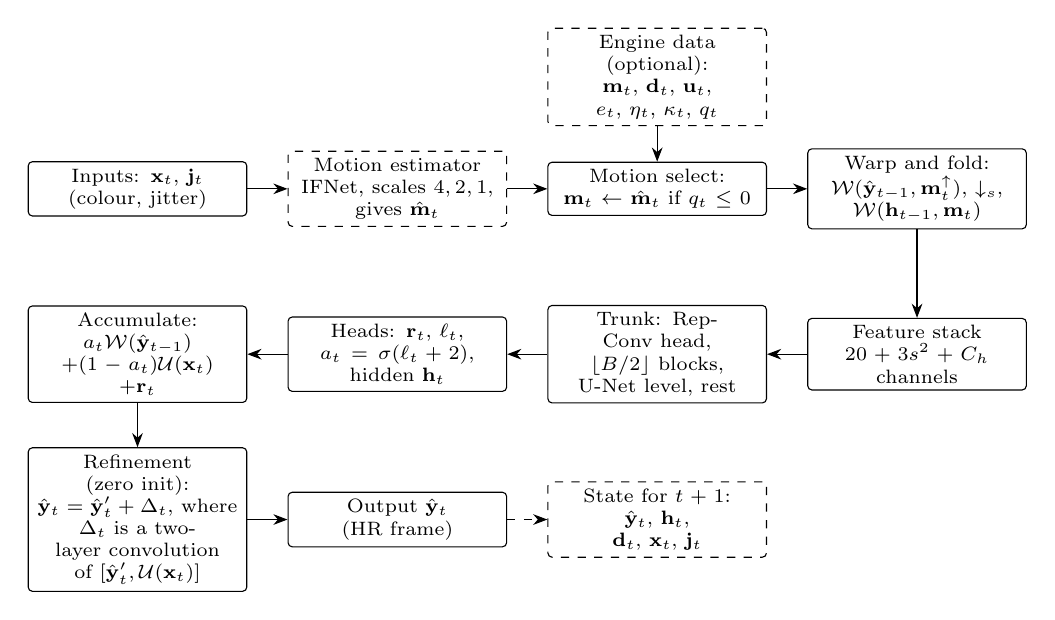
\begin{tikzpicture}[font=\scriptsize, node distance=0pt,
  box/.style={draw, rounded corners=1.5pt, align=center, text width=2.6cm, inner sep=2.5pt},
  opt/.style={box, dashed},
  arr/.style={-{Stealth[length=1.8mm]}},
  rec/.style={-{Stealth[length=1.8mm]}, dashed}]
\node[box] (in) at (0,6.0) {Inputs: $\mathbf{x}_t$, $\mathbf{j}_t$\\(colour, jitter)};
\node[opt] (est) at (3.3,6.0) {Motion estimator\\IFNet, scales $4,2,1$,\\gives $\hat{\mathbf{m}}_t$};
\node[box] (sel) at (6.6,6.0) {Motion select:\\$\mathbf{m}_t\leftarrow\hat{\mathbf{m}}_t$ if $q_t\le 0$};
\node[box] (warp) at (9.9,6.0) {Warp and fold:\\$\mathcal{W}(\hat{\mathbf{y}}_{t-1},\mathbf{m}_t^{\uparrow})$, $\downarrow_s$,\\$\mathcal{W}(\mathbf{h}_{t-1},\mathbf{m}_t)$};
\node[opt, above=0.45cm of sel] (eng) {Engine data (optional):\\$\mathbf{m}_t$, $\mathbf{d}_t$, $\mathbf{u}_t$,\\$e_t$, $\eta_t$, $\kappa_t$, $q_t$};
\node[box] (stack) at (9.9,3.9) {Feature stack\\$20+3s^2+C_h$ channels};
\node[box] (trunk) at (6.6,3.9) {Trunk: RepConv head,\\$\lfloor B/2\rfloor$ blocks,\\U-Net level, rest};
\node[box] (heads) at (3.3,3.9) {Heads: $\mathbf{r}_t$, $\ell_t$,\\$a_t=\sigma(\ell_t+2)$,\\hidden $\mathbf{h}_t$};
\node[box] (acc) at (0,3.9) {Accumulate:\\$a_t\mathcal{W}(\hat{\mathbf{y}}_{t-1})$\\$+(1-a_t)\mathcal{U}(\mathbf{x}_t)$\\$+\mathbf{r}_t$};
\node[box] (refine) at (0,1.8) {Refinement (zero init):\\$\hat{\mathbf{y}}_t=\hat{\mathbf{y}}'_t+\Delta_t$, where\\$\Delta_t$ is a two-layer convolution\\of $[\hat{\mathbf{y}}'_t,\mathcal{U}(\mathbf{x}_t)]$};
\node[box] (out) at (3.3,1.8) {Output $\hat{\mathbf{y}}_t$\\(HR frame)};
\node[opt] (state) at (6.6,1.8) {State for $t+1$:\\$\hat{\mathbf{y}}_t$, $\mathbf{h}_t$,\\$\mathbf{d}_t$, $\mathbf{x}_t$, $\mathbf{j}_t$};
\draw[arr] (in) -- (est);
\draw[arr] (est) -- (sel);
\draw[arr] (sel) -- (warp);
\draw[arr] (eng) -- (sel);
\draw[arr] (warp) -- (stack);
\draw[arr] (stack) -- (trunk);
\draw[arr] (trunk) -- (heads);
\draw[arr] (heads) -- (acc);
\draw[arr] (acc) -- (refine);
\draw[arr] (refine) -- (out);
\draw[rec] (out) -- (state);
\end{tikzpicture}
\caption{Data flow of one TSR time step at scale $s$. Dashed boxes are optional: the engine data are used when the caller supplies them, and the estimator runs in training for every frame and at inference only when a sample has no motion. The state of frame $t$ holds the history, hidden state, depth, colour and jitter that the warp and disocclusion cue of frame $t+1$ read (\cref{sec:tsrm-state})}\label{fig:tsrm-arch}
\end{figure}

\FloatBarrier

\subsection{Inputs}\label{sec:tsrm-inputs}

The trunk receives a stack of channels at render resolution. \Cref{tab:tsrm-inputs} lists them in the order of the code. Seventeen channels come from the frame and its side information, $3s^2$ from the folded history, three from the history disagreement and $C_h$ from the hidden state, so the stack has $20+3s^2+C_h$ channels. For $s=3$ and $C_h=8$ this is $55$, which the code confirms for the \tier{low} tier. The table gives the value that the network sees in each mode. Two replacements happen before the stack is built. A sample without motion receives the estimate $\hat{\mathbf{m}}_t$ and the flag $0.25$ (\cref{sec:tsrm-motion}). A sample with withheld depth receives zero depth and $\eta_t=0$.

The engine motion of the table is the motion in the input, which is exact (synthetic, TartanAir and Sintel), RAFT (real video and GameIR), or absent. The value $\tfrac12$ marks RAFT motion and video samples that keep their motion labels, which are capped at $\tfrac12$ by the degradation of \cref{sec:tsrm-data}.

The depth normalisation of \cref{tab:tsrm-inputs} is
\begin{equation}\label{eq:tsrm-depth}
\mathbf{d}_t=\frac{1}{1+\mathbf{d}^{\mathrm{raw}}_t/\operatorname{med}(\mathbf{d}^{\mathrm{raw}})},
\end{equation}
where $\mathbf{d}^{\mathrm{raw}}$ is the depth in the unit of its source, and $\operatorname{med}$ is the median over the whole sequence for synthetic samples, and over one frame for real windows and test clips. Non-positive and non-finite depth values are set to infinity before the normalisation, so they map to values near zero.

The normals are derived from the normalised depth with edge replication at the border, using the central differences $g^x_t(X,Y)=8\,[\mathbf{d}_t(X+1,Y)-\mathbf{d}_t(X-1,Y)]$ and $g^y_t$ defined in the same way along $Y$:
\begin{equation}\label{eq:tsrm-normal}
\mathbf{n}_t=\eta_t\,\frac{(-g^x_t,\,-g^y_t,\,1)}{\sqrt{(g^x_t)^2+(g^y_t)^2+1}}.
\end{equation}
The factor $8$ is a fixed constant of the code that scales the depth gradient, and the vector is normalised to unit length.

The disocclusion cue compares the current depth with the depth of the previous frame warped to the current frame, using the motion of the network:
\begin{equation}\label{eq:tsrm-disocc}
\delta_t=\eta_t\,\min\Big\{1,\ \frac{\lvert\mathbf{d}_t-\mathcal{W}(\mathbf{d}_{t-1},\mathbf{m}_t)\rvert}{\lvert\mathbf{d}_t\rvert+10^{-3}}\Big\}.
\end{equation}
A large value marks a depth that differs from the warped previous depth, which is typical of a disocclusion. It is a heuristic that the trunk refines, not a visibility test.

\subsection{Motion estimator}\label{sec:tsrm-motion}

The estimator is the IFNet of RIFE 4.26 \cite{huang2022rife} in a narrower form, a coarse-to-fine chain of flow blocks. It is built by \texttt{IFNet(widths, n\_res, n\_hint=3)} in \texttt{nss\_models.py}. Its widths and residual counts are set per tier in the constant \texttt{TSR\_TIERS}: $(32,24,16)$ with two residual blocks for \tier{igpu}, $(48,32,24)$ with three for \tier{low}, $(64,48,32)$ with four for \tier{mid}, $(96,64,48)$ with four for \tier{high}, and $(128,96,64)$ with six for \tier{teacher}. The three levels run at scales $\sigma_1=4$, $\sigma_2=2$ and $\sigma_3=1$ relative to the LR frame, so the coarsest block sees a frame of a quarter of the LR size in each direction.

The estimator takes the previous colour frame $\mathbf{x}_{t-1}$ and the current frame $\mathbf{x}_t$, both padded at the right and bottom by edge replication to multiples of $16$. Its timestep is the constant $1$, so its target frame is the current frame and its reference is the previous one. Its final flow, the first two of its four channels, is the motion of \cref{sec:tsrm-problem}:
\begin{equation}\label{eq:tsrm-est}
\hat{\mathbf{m}}_t=\mathbf{F}^{(3)}_{0},\qquad \mathbf{F}^{(1)}=\Delta^{(1)},\qquad \mathbf{F}^{(k)}=\mathbf{F}^{(k-1)}+\Delta^{(k)}\ \ (k=2,3),
\end{equation}
where $\Delta^{(k)}$ is the four-channel flow update of block $k$ and $\mathbf{F}^{(k)}=(\mathbf{F}^{(k)}_0,\mathbf{F}^{(k)}_1)$ holds the flows from the target to the previous and to the current frame. The flow outputs are multiplied by the block scale, so the flows stay in LR pixels.

The first block receives $\mathbf{x}_{t-1}$, $\mathbf{x}_t$, the per-frame features of both frames and the constant timestep, which is $15$ channels. Each later block receives the colour of both frames warped by the current flow, the features of both frames warped by the current flow, the timestep, the blend mask and the features of the previous block, and the current flow itself, which is $28$ channels. Three hint channels follow for the TSR estimator: the jitter difference $\mathbf{j}_t-\mathbf{j}_{t-1}$ (two channels) and the input kind $\kappa_t$ (one channel). The per-frame feature encoder has a stride-two $3\times3$ convolution and two $3\times3$ convolutions, each followed by LeakyReLU, and a transposed convolution that returns to full resolution with four channels. Inside each block, two stride-two $3\times3$ convolutions reduce the resolution by four, a set of residual $3\times3$ convolutions with a learned per-channel scale follows, and a transposed convolution with pixel shuffle returns to the block resolution with $4$ flow channels, one mask logit and $8$ features.

The estimator is initialised from the RIFE 4.26 weights wherever the names match, and its narrower layers take the leading channel slices of the RIFE tensors. The weight loader \texttt{load\_ifnet\_weights} copies the matching tensors whole and the narrower ones as slices, and the hint channels keep their zero weights. The training log of the \tier{low} run records the result as 11 whole tensors and 42 sliced tensors with no missing tensor. Without the RIFE weights, the code falls back to random initialisation and logs the fact.

The estimate replaces the motion only where the caller gave none. The rule is the one line of \texttt{TSRNet.forward}:
\begin{equation}\label{eq:tsrm-select}
\mathbf{m}_t=\begin{cases}\bar{\mathbf{m}}_t\ \text{(teacher-forced label)} & \text{if } q_t\le 0 \text{ and the sample is forced},\\ \hat{\mathbf{m}}_t & \text{if } q_t\le 0 \text{ otherwise},\\ \text{given motion} & \text{if } q_t>0,\end{cases}
\end{equation}
and the quality flag of every sample with $q_t\le 0$ becomes $\tfrac14$ (the constant \texttt{EST\_MV\_QUALITY}). The flag is therefore the same for estimated and forced samples, and the network cannot tell them apart. At inference the estimator runs only when some sample of the batch has $q_t\le 0$. In training it runs for every frame of every sample, because the motion loss of \cref{sec:tsrm-loss} supervises every sample that has a label, including those with engine motion.

Teacher forcing protects the trunk while the estimator is still poor. A sample without motion is forced to warp its history with the label motion $\bar{\mathbf{m}}_t$ with probability $\pi(\tau)$, drawn once per sample and used for all its frames, where $\tau$ is the elapsed training time and $T_b$ the training budget in seconds:
\begin{equation}\label{eq:tsrm-teacher}
\pi(\tau)=\max\Big(0,\ 1-\frac{\tau}{\rho\,T_b}\Big),\qquad \rho=\Res{tsr.config.cfg.mv_warmup_frac}.
\end{equation}
The forcing applies only to samples that have a label, so $\lambda>0$. Its probability falls linearly from one to zero over the first quarter of the budget, after which no forced mask is drawn. The clock is the wall-clock time of each process from its first step, so the two DDP ranks draw their masks on their own clocks. Teacher forcing is the name for feeding a recurrent predictor a target in place of its own output during training. Here it is this code's schedule, which replaces the estimate by the label for part of the early training only.

\subsection{Warping, folding and the recurrent state}\label{sec:tsrm-state}

The state carried from frame $t-1$ to frame $t$ is
\begin{equation}\label{eq:tsrm-state}
\mathcal{S}_{t-1}=\big(\hat{\mathbf{y}}_{t-1},\ \mathbf{h}_{t-1},\ \mathbf{d}_{t-1},\ \mathbf{x}_{t-1},\ \mathbf{j}_{t-1}\big).
\end{equation}
The depth, colour and jitter are kept for the disocclusion cue and for the estimator of frame $t$. The ONNX export passes them as explicit inputs (\cref{sec:tsrm-deploy}).

The previous output is warped to the HR grid with the upsampled motion. The LR motion is interpolated bilinearly to HR and multiplied by the scale, because a displacement of $d$ LR pixels is $sd$ HR pixels:
\begin{equation}\label{eq:tsrm-up-motion}
\mathbf{m}_t^{\uparrow}=s\cdot\mathrm{Bil}^{\times s}[\mathbf{m}_t],\qquad \mathbf{H}_t=\mathcal{W}\big(\hat{\mathbf{y}}_{t-1},\mathbf{m}_t^{\uparrow}\big),
\end{equation}
where $\mathrm{Bil}^{\times s}$ is bilinear upsampling by $s$ with align-corners set to false. The folded history is $\downarrow_s\mathbf{H}_t\in\mathbb{R}^{3s^2\times h\times w}$, the space-to-depth rearrangement of PyTorch's pixel unshuffle, which places every $s\times s$ block of HR pixels in the channels of one LR pixel. The history disagreement uses the mean of each block, $\bar{\mathbf{H}}_t=\operatorname{avgpool}_s(\mathbf{H}_t)$, and its absolute difference to the LR colour, $\mathbf{g}_t=\lvert\bar{\mathbf{H}}_t-\mathbf{x}_t\rvert$.

The hidden state and the depth are warped at LR with the LR motion $\mathbf{m}_t$, which is the motion of the network. The hidden state after frame $t$ is produced by the trunk, as \cref{sec:tsrm-output} gives. Warping uses the backward warp of \cref{eq:tsrm-warp}:
\begin{equation}\label{eq:tsrm-warp}
\mathcal{W}(I,\mathbf{m})(\mathbf{p})=I\big(\mathbf{p}+\mathbf{m}(\mathbf{p})\big),
\end{equation}
where $I$ is read bilinearly and clamped to its border. The implementation uses grid sampling with align-corners set to true, the convention of RIFE, so that the pixel centres of the first and last rows and columns lie on the image border.

On the first frame of a sequence, or in every frame of the no-history ablation, the state is empty. The history $\mathbf{H}_t$, the folded history, the history disagreement and the warped hidden state are all multiplied by zero, the disocclusion cue is computed against the current depth so that it is zero, and the history weight is set to zero exactly, not learned, by the rule
\begin{equation}\label{eq:tsrm-reset}
a_t=0\quad\text{when the state is empty.}
\end{equation}
The network has no other reset. It has no scene-cut detector, so the history weight must reject a cut by itself. The synthetic renderer produces no cuts, and the cache builders contain no cut filter, so a real window may contain a cut, and the training does not measure how often that happens.

\subsection{Reconstruction trunk}\label{sec:tsrm-trunk}

The trunk is a chain of re-parameterisable blocks, called RepConv here, in the sense of RepVGG \cite{ding2021repvgg} and ECBSR \cite{zhang2021ecbsr}. A RepConv block is trained as a sum of linear branches and deployed as one $3\times3$ convolution. A training forward pass folds the branches into one kernel on every call, so each block costs one convolution in training and one in deployment. The folded kernel for an output channel $o$ and an input channel $i$ is
\begin{equation}\label{eq:tsrm-fold}
\mathbf{W}_{oi}=\mathbf{W}^{(3)}_{oi}+\operatorname{pad}_{3\times3}\big(\mathbf{W}^{(1)}_{oi}\big)+\sum_{k=1}^{3}\mathbf{P}_{o,i,k}\,\mathbf{E}_k+\delta_{oi}\,\mathbf{C},
\end{equation}
with the bias $b_o=b^{(3)}_o+b^{(1)}_o+b^{(e)}_o$. The symbols are as follows. $\mathbf{W}^{(3)}$ is a learned $3\times3$ kernel and $\mathbf{W}^{(1)}$ a learned $1\times1$ kernel, padded with zeros to $3\times3$. The matrices $\mathbf{E}_1$, $\mathbf{E}_2$ and $\mathbf{E}_3$ are the fixed Sobel-x, Sobel-y and Laplacian kernels, $[[-1,0,1],[-2,0,2],[-1,0,1]]$, $[[-1,-2,-1],[0,0,0],[1,2,1]]$ and $[[0,1,0],[1,-4,1],[0,1,0]]$. The coefficients $\mathbf{P}_{o,i,k}$ form a learned $1\times1$ convolution from $3C_i$ inputs to $C_o$ outputs, reshaped so that each input channel $i$ has its three edge responses $k$. The matrix $\mathbf{C}$ has a one at its centre and zeros elsewhere, and the term with $\delta_{oi}$ is present only when $C_i=C_o$. Because the folding is linear, the folded convolution computes exactly the same function as the training branches.

Each RepConv is followed by a PReLU with one learned slope per output channel, initialised to PyTorch's default of $0.25$. The side branches start at zero, in the following sense. The weights of the $1\times1$ branch and of the edge branch are set to zero, so the block starts as a $3\times3$ convolution plus identity. Their biases keep PyTorch's default uniform initialisation, so the side branches do not start exactly at zero. The code records that default initialisation grew the activations by about $1.9$ times per block and gave a non-finite teacher loss from step $10$ in an earlier run \Observation.

The trunk of \cref{eq:tsrm-trunk-def} is built from the stack $\mathbf{z}_t$, which has $20+3s^2+C_h$ channels. Let $\mathrm{RC}_{\mathrm{head}}$ denote the head RepConv block, $\mathcal{A}$ the first $\lfloor B/2\rfloor$ blocks, $\mathcal{B}$ the remaining $B-\lfloor B/2\rfloor$ blocks, and $\mathcal{V}$ the U-Net level, which exists when $U>0$:
\begin{align}
\mathbf{z}_0&=\mathrm{RC}_{\mathrm{head}}(\mathbf{z}_t) \label{eq:tsrm-trunk-def}\\
\mathbf{z}_1&=\mathcal{A}(\mathbf{z}_0)\nonumber\\
\mathbf{z}_2&=\mathbf{z}_1+\mathcal{V}(\mathbf{z}_1)\nonumber\\
\mathbf{y}_t&=\mathcal{B}(\mathbf{z}_2).\nonumber
\end{align}
The head is one RepConv from $20+3s^2+C_h$ channels to $C$ channels. The U-Net level, when present, is a $3\times3$ convolution with stride two from $C$ to $2C$ channels followed by PReLU, then $U$ RepConv blocks at $2C$ channels, then a $1\times1$ convolution from $2C$ to $4C$ channels and a pixel shuffle with factor two, which returns $C$ channels at LR resolution. The U-Net level therefore works at half the LR resolution and is added to the trunk as a residual. The LR input is padded to an even size by edge replication before the trunk, which the stride-two convolution needs. The numbers of blocks per tier are in \cref{tab:tsrm-tiers}.

\subsection{Output head and accumulation}\label{sec:tsrm-output}

The output head is one $3\times3$ convolution from $C$ to $4s^2$ channels, with zero weights and zero bias, applied to $\mathbf{y}_t$. A pixel shuffle with factor $s$ \cite{shi2016espcn} then gives four channels at HR. The first three are the residual $\mathbf{r}_t$ and the fourth is a logit $\ell_t$, and the history weight is
\begin{equation}\label{eq:tsrm-alpha}
a_t=\sigma(\ell_t+2),\qquad \sigma(z)=\frac{1}{1+e^{-z}}.
\end{equation}
At initialisation the zero weights give $\ell_t=0$, so $a_t=\sigma(2)\approx0.881$ and $\mathbf{r}_t=0$, and the network starts as a blend of the warped history and the upsampled colour. The hidden state is produced by a $3\times3$ convolution from $C$ to $C_h$ channels followed by $\tanh$, $\mathbf{h}_t=\tanh(\mathrm{Conv}_{3\times3}(\mathbf{y}_t))$, and it is warped at the next frame by \cref{eq:tsrm-warp}.

The output is the accumulation rule
\begin{equation}\label{eq:tsrm-acc}
\hat{\mathbf{y}}'_t=a_t\odot\mathcal{W}\big(\hat{\mathbf{y}}_{t-1},\mathbf{m}_t^{\uparrow}\big)+(1-a_t)\odot\mathcal{U}(\mathbf{x}_t)+\mathbf{r}_t,
\end{equation}
where $\odot$ is the element-wise product, $\mathcal{U}$ is the jitter-aware bilinear upsampling
\begin{equation}\label{eq:tsrm-up}
\mathcal{U}(\mathbf{x}_t)(X,Y)=\operatorname{Bil}[\mathbf{x}_t]\Big(\frac{X+\tfrac12}{s}-\mathbf{j}_t\Big),
\end{equation}
and $\operatorname{Bil}[\mathbf{x}]$ is the bilinear interpolant of the LR samples, sample $i$ at coordinate $i+\tfrac12$, with clamped borders. The term $\frac{X+1/2}{s}$ is the continuous LR coordinate of output pixel $(X,Y)$, and subtracting $\mathbf{j}_t$ reads each LR sample at its jittered position. The output is then refined as \cref{sec:tsrm-refine} gives. On the first frame, $a_t=0$ by \cref{eq:tsrm-reset}, so $\hat{\mathbf{y}}_0=\mathcal{U}(\mathbf{x}_0)+\mathbf{r}_0$.

\paragraph{Why this is a learned temporal accumulation.} Ignore the residual and the motion for a moment, and let $a_t=a$ be constant, with $\mathbf{m}_t=0$ on a static scene. Then \cref{eq:tsrm-acc} unrolls to
\begin{equation}\label{eq:tsrm-unroll}
\hat{\mathbf{y}}_t=a^{t}\,\mathcal{U}(\mathbf{x}_0)+\sum_{k=1}^{t}(1-a)\,a^{t-k}\,\mathcal{U}(\mathbf{x}_k).
\end{equation}
The weights add to one, because $a^t+(1-a)\sum_{j=0}^{t-1}a^j=a^t+(1-a^t)=1$. The sample $k$ frames old has weight $(1-a)a^{k}$, which is an exponential moving average over the frames of the sequence, with mean age $a/(1-a)$ frames. Each $\mathcal{U}(\mathbf{x}_k)$ reads the colour at a different sub-pixel jitter, so the average gathers the samples of several sub-pixel positions. This is the principle of temporal accumulation for supersampling \cite{yang2020taasurvey} (\cref{sec:bg-taa}). At the initial history weight $\sigma(2)$ the mean age is about $7.4$ frames.

Classical TAA has the same update with a fixed or heuristic blend weight, and it rectifies the reprojected history by clamping it to the colour neighbourhood of the current frame. \Cref{eq:tsrm-acc} keeps the update and changes the rectification. The weight $a_t$ is a learned per-pixel gate, and the network has the disagreement $\mathbf{g}_t$ as input and a receptive field of several convolutions, so the gate can learn to go to zero where the history is invalid, which happens at disocclusions and at particle effects. The residual $\mathbf{r}_t$ corrects the result additively. There is no explicit clamp anywhere in the TSR network, so the residual can move a pixel outside the neighbourhood of the current frame. The analytic baseline of \cref{sec:tsrm-test} does clamp, and the two rectifications are different.

\subsection{Refinement and the reset rule}\label{sec:tsrm-refine}

Every tier except \tier{igpu} refines the accumulated output at HR resolution. The refinement is
\begin{equation}\label{eq:tsrm-refine}
\hat{\mathbf{y}}_t=\hat{\mathbf{y}}'_t+\mathrm{Conv}_{3\times3}\Big(\mathrm{PReLU}\big(\mathrm{Conv}_{3\times3}([\hat{\mathbf{y}}'_t,\mathcal{U}(\mathbf{x}_t)])\big)\Big),
\end{equation}
where $[\cdot,\cdot]$ concatenates six channels. The first convolution has $R$ output channels and the second has three. The second convolution has zero weights and zero bias, so the refinement starts at the identity. Its purpose is to remove the pixel-shuffle pattern of the LR head, as the code comment states. The width $R$ is $8$ for \tier{low} and \tier{mid}, $12$ for \tier{high} and $16$ for the teacher, and the \tier{igpu} tier has no refinement.

The reset rule is \cref{eq:tsrm-reset}. It applies to the first frame of each training window and each test clip, and in every frame of the no-history ablation (\cref{sec:tsrm-abl}). The ONNX step of \cref{sec:tsrm-deploy} has no reset input.

\subsection{Model tiers}\label{sec:tsrm-tiers}

The tiers are the entries of \texttt{TSR\_TIERS} in \texttt{nss\_models.py}. \Cref{tab:tsrm-tiers} gives their widths, block counts, U-Net blocks, hidden widths, estimator, refinement width, parameter counts and costs. The parameter counts are those of the fused network, with the estimator included, and the estimator parameters are the difference from the same network built without the estimator. The costs count multiply-accumulates of every convolution, including the estimator, for one steady-state frame with history, per 1080p output frame, and exclude the warps and the pixel shuffles, which have no multiply-accumulates. The counting is done with forward hooks on the fused network in \texttt{tsr\_macs\_per\_lr\_pixel}, and the notebook scales it by the LR pixel count.

The fused parameter counts and the 3x and 2x costs are the values that \texttt{model\_tiers.csv} records for the run. They were also recomputed from \texttt{src/neuralss/nss\_models.py} on the current code, and both agree. The estimator column is the difference between the training parameter count with and without the estimator, which is also computed from the code. The \tier{mid} and \tier{high} tiers are defined and costed, but the TSR notebook never trains them. Its runs use the teacher at 3x, \tier{low} at 3x and 2x, \tier{igpu} at 3x, and the six ablation runs at 3x, which all use \tier{low}. The tier table of the article (\cref{M-tab:tiers}) therefore gives no latency for these two tiers.

The estimator holds a large share of the training parameters of every tier. It is about $81$ percent for \tier{igpu}, $63$ percent for \tier{low} and $51$ percent for the teacher, and it runs on every frame without engine motion.

\subsection{Training samples and degradations}\label{sec:tsrm-data}

Each training step draws from two streams, and both produce sequences of $T$ frames with HR targets, LR inputs, motion labels and validity masks. The synthetic stream renders layered game-like scenes from cached texture crops with the renderer of \cref{sec:data-synth}. Its scene parameters, which are used here, are a background layer and a foreground layer with procedural alpha (a superellipse, four thin wires each present with probability $0.6$, and a fence present with probability $0.35$), moving on continuous affine paths. The foreground texture is flat with probability $0.25$ and is otherwise the still of the neighbouring sample in the batch, the foreground layer is present with probability $0.85$, world-space text tiles are stamped into the background with probability $0.3$, and six particles are drawn, each active with probability $0.5$. The motion class is static, slow, medium or fast with probabilities $0.15$, $0.45$, $0.25$ and $0.15$, which give speeds of $0$, $0.3$ to $3$, $3$ to $10$ and $10$ to $28$ output pixels per frame. Each sample has an exposure $2^{u}$ with $u$ uniform on $[-0.8,0.8]$, and a sub-pixel jitter phase drawn uniformly from the sixteen Halton offsets. The LR frames are single-sample jittered reads of the renderer, and the HR targets are four-sample renders.

The real stream reads cached windows of $T$ frames at $P=192$ output pixels from the sequence sources of \cref{sec:data}. The window is drawn from a source-specific downscale range before cropping. A real window is flipped horizontally with probability $\tfrac12$ and vertically with probability $\tfrac12$, and its motion vectors are negated in the flipped components. It is scaled in linear light by an exposure gain $2^{u}$ with $u$ uniform on $[-0.8,0.8]$. Its LR frames are jittered bilinear reads of the HR frame, so they are aliased like a render. The labels are the cached motion and validity, with the label quality of the window. Exact motion, from TartanAir and Sintel, has label quality $1$. Other windows get RAFT motion when RAFT is available, with label quality $\tfrac12$, and otherwise zero motion with label quality $0$. \Cref{tab:tsrm-mix} lists the probabilities that the TSR configuration or the degradation functions set.

\begin{table}[!htbp]
\caption{Probabilities of the TSR training data that are set by the TSR configuration or by the degradation functions. The renderer's own probabilities are given in \cref{sec:tsrm-data} and \cref{sec:data-synth}}\label{tab:tsrm-mix}
{\scriptsize\raggedright\setlength{\tabcolsep}{3pt}
\begin{tabular*}{\textwidth}{@{\extracolsep\fill}p{0.44\textwidth}p{0.16\textwidth}p{0.32\textwidth}}
\toprule
Quantity & Value & Code location \\
\midrule
Real windows per batch & $\Res{tsr.config.cfg.p_real}$, so $19$ of $48$ & \texttt{p\_real}, \texttt{make\_loader} \\
Synthetic samples turned into plain video & $\Res{tsr.config.cfg.p_video_synth}$ & \texttt{p\_video\_synth}, \texttt{video\_degrade} \\
Real samples turned into plain video & $\Res{tsr.config.cfg.p_video_real}$ & \texttt{p\_video\_real}, \texttt{video\_degrade} \\
Plain-video samples that keep their motion labels & $\Res{tsr.config.cfg.p_video_mv}$ & \texttt{p\_video\_mv}, \texttt{video\_degrade} \\
Samples that lose their motion vectors (all samples of the batch) & $\Res{tsr.config.cfg.p_drop_mv}$ & \texttt{p\_drop\_mv}, \texttt{withhold\_engine\_data} \\
Samples that lose their depth (all samples of the batch) & $\Res{tsr.config.cfg.p_drop_depth}$ & \texttt{p\_drop\_depth}, \texttt{withhold\_engine\_data} \\
Long steps, every fourth step from step $0$ & $1/\Res{tsr.config.cfg.long_every}$ & \texttt{long\_every} $=\Res{tsr.config.cfg.long_every}$, \texttt{train\_tsr.step\_fn} \\
Teacher forcing of motion & $\pi(\tau)$ in \cref{eq:tsrm-teacher} & \texttt{mv\_warmup\_frac} $=\Res{tsr.config.cfg.mv_warmup_frac}$ \\
Horizontal and vertical flip of real windows & $1/2$ each & \texttt{sr\_batch\_from\_frames} \\
Gain of real windows and scene exposure & $2^{u}$, $u\sim U[-0.8,0.8]$ & \texttt{sr\_batch\_from\_frames}, \texttt{Scene} \\
Downscale filter of plain video (bicubic, bilinear, box) & $1/3$ each & \texttt{video\_lr} \\
Blur $\sigma$ of plain video & $U[0,0.6]$ output pixels & \texttt{video\_lr} \\
Noise $\sigma$ of plain video & $U[0,2/255]$ & \texttt{video\_lr} \\
\botrule
\end{tabular*}}
\end{table}

The plain-video degradation turns a sample into ordinary video. A plain-video LR frame is the target frame $\mathbf{y}$ after a Gaussian blur, an anti-aliased downscale, additive noise and 8-bit quantisation. The blur is a five-tap separable Gaussian on the output grid with $\sigma$ uniform on $[0,0.6]$. The downscale $D$ is bicubic (cubic convolution \cite{keys1981bicubic}), bilinear or box averaging, each chosen with probability $1/3$. The noise is added after the downscale, with $\sigma_n$ uniform on $[0,2/255]$, and the frame is clamped and rounded to multiples of $1/255$:
\begin{equation}\label{eq:tsrm-video}
\mathbf{x}^{\mathrm{vid}}_t=\mathrm{round}_{1/255}\Big(\mathrm{clip}_{[0,1]}\big(D\big(G_\sigma\ast\mathbf{y}_t\big)+\mathbf{n}\big)\Big),\qquad \mathbf{n}\sim\mathcal{N}(0,\sigma_n^2 I).
\end{equation}
A plain-video sample loses its jitter, its depth, its reactive mask and its depth availability, and its input kind becomes $\kappa_t=0$. Its motion is removed, except for the share $p_\mathrm{mv}=0.15$ that keeps the label motion with flag $\min(q,\tfrac12)$. The label motion of a plain-video sample is the block mean of the HR motion, divided by $s$, and its validity is one only where all $s\times s$ HR pixels are valid. The labels keep their label quality, so a plain-video sample still supervises the estimator.

The withholding rule is applied to the whole batch after both streams are built. Its two masks are drawn once per sample and apply to every sample, including the plain-video samples that kept their motion. A sample loses its motion with probability $0.25$, and it loses its depth with probability $0.3$. A plain-video sample that kept its motion therefore loses it with probability $0.25$.

Most real windows come from Vimeo-90K \cite{xue2019vimeo}, and only a small share has exact motion, as \cref{M-sec:discussion} reports \UnderRevision. The configuration gives the cache capacities of \Res{tsr.config.cfg.cache.still_train} still crops and \Res{tsr.config.cfg.cache.win_train} windows.

\subsection{Unroll lengths and patch sizes}\label{sec:tsrm-unroll}

Each training window has $T=\Res{tsr.config.cfg.seq_len}$ frames of $P=\Res{tsr.config.cfg.patch}$ output pixels, which is $64$ LR pixels at $s=3$ and $96$ at $s=2$. The network runs through the frames of a window in order, the state starts empty, and the loss of every frame is summed before one backward pass. The gradient flows through every frame of the window, and it stops at the window boundary, which is truncated back-propagation through time \cite{williams1990efficient}. The notebook gives six frames per window, as truncated back-propagation through the recurrence, and 192-pixel patches as its defaults. It sets $\Res{tsr.config.cfg.still_size}$-pixel texture crops so that fast camera paths have room inside the texture.

Every fourth step is a long step with $T=\Res{tsr.config.cfg.long_t}$ frames of $P=\Res{tsr.config.cfg.long_patch}$ pixels, which is $16\times96^2=147{,}456$ output pixels per window, two thirds of the $6\times192^2=221{,}184$ of a normal window. The notebook gives the reason for the long steps as the decline of the earlier students on static scenes after frames $6$ to $10$, which the notebook measured in one earlier run \Preliminary. The long steps use only synthetic windows, so each GPU has $48-19=29$ of them in a long step, against $48$ windows in a normal step.

The batch is $48$ windows per GPU for the teacher and for the students. The batch probe of the notebook tried sizes $4$, $8$, $12$, $16$, $24$, $32$ and $48$, and it kept the largest size that stayed below $75$ percent of GPU memory. Both models passed at $48$ with memory use well below that limit, so the list, not the memory, set the batch. The main stages run on both GPUs with distributed data parallel, which gives $96$ windows per step, and the paired runs and ablations run on one GPU each, with $48$ windows per step.

\subsection{Loss}\label{sec:tsrm-loss}

The loss is computed for every window and then averaged over the batch. For the frames $t=0,\dots,T-1$ of a window, let $\hat{\mathbf{y}}_t$ be the output and $\mathbf{y}_t$ the target. The pixel term is a Charbonnier penalty, with $\varepsilon=10^{-3}$, averaged over the frames with weight $\tfrac14$ on the first frame, which has no history:
\begin{equation}\label{eq:tsrm-lpix}
\mathcal{L}_\mathrm{pix}=\frac{\sum_{t}\omega_t\,\mathbb{E}\sqrt{(\hat{\mathbf{y}}_t-\mathbf{y}_t)^2+\varepsilon^2}}{\sum_t\omega_t},\qquad \omega_0=\tfrac14,\ \ \omega_t=1\ \ (t\ge1).
\end{equation}
The expectation $\mathbb{E}$ is the mean over the channels and pixels of the batch. The Charbonnier penalty \cite{charbonnier1997deterministic} is a smooth edge-preserving potential that approximates the absolute difference.

The gradient term compares the finite differences of the output and the target over a distance of two pixels in each direction. With $D_x\mathbf{z}(X,Y)=\mathbf{z}(X+2,Y)-\mathbf{z}(X,Y)$ and $D_y$ defined in the same way along $Y$,
\begin{equation}\label{eq:tsrm-lgrad}
\mathcal{L}_\mathrm{grad}=\mathbb{E}_t\big|D_x\hat{\mathbf{y}}_t-D_x\mathbf{y}_t\big|+\mathbb{E}_t\big|D_y\hat{\mathbf{y}}_t-D_y\mathbf{y}_t\big|,
\end{equation}
where $\mathbb{E}_t$ is the mean over all frames of the window, the channels and the pixels.

The Fourier term compares the magnitudes of the two-dimensional spectra of the frames, computed with the orthonormal real FFT, so that texture energy at every frequency counts:
\begin{equation}\label{eq:tsrm-lfft}
\mathcal{L}_\mathrm{fft}=\mathbb{E}_t\Big|\,\big|\mathcal{F}\hat{\mathbf{y}}_t\big|-\big|\mathcal{F}\mathbf{y}_t\big|\,\Big|,
\end{equation}
where $\mathcal{F}$ is the orthonormal real two-dimensional FFT of each channel and $|\cdot|$ is the complex magnitude.

The temporal term matches the change of the output to the change of the target along the label motion, at HR, over the pixels that are visible in both frames:
\begin{multline}\label{eq:tsrm-ltmp}
\mathcal{L}_\mathrm{tmp}=\frac{1}{T-1}\sum_{t=1}^{T-1}\frac{\sum_{\mathbf{p}}\bar{\mathbf{V}}_t(\mathbf{p})\,\lambda_t\sum_{c}\big|\Delta^{\mathrm{out}}_{t,c}(\mathbf{p})-\Delta^{\mathrm{gt}}_{t,c}(\mathbf{p})\big|}{3\sum_{\mathbf{p}}\bar{\mathbf{V}}_t(\mathbf{p})\,\lambda_t+10^{-6}},
\end{multline}
where $\Delta^{\mathrm{out}}_t=\hat{\mathbf{y}}_t-\mathcal{W}(\hat{\mathbf{y}}_{t-1},\bar{\mathbf{M}}_t)$ and $\Delta^{\mathrm{gt}}_t=\mathbf{y}_t-\mathcal{W}(\mathbf{y}_{t-1},\bar{\mathbf{M}}_t)$ are the temporal changes of the output and of the target along the label motion, $\bar{\mathbf{M}}_t$ is the HR label motion, $\bar{\mathbf{V}}_t$ its validity and $\lambda_t$ its label quality. The term is zero for windows without labels.

The motion term supervises the estimator on every frame after the first, with the LR label motion $\bar{\mathbf{m}}_t$ and its validity $\bar{\mathbf{v}}_t$:
\begin{equation}\label{eq:tsrm-lflow}
\mathcal{L}_\mathrm{flow}=\frac{\sum_{t=1}^{T-1}\sum_{\mathbf{p}}\lambda_t\,\bar{\mathbf{v}}_t(\mathbf{p})\,\big\lVert\hat{\mathbf{m}}_t(\mathbf{p})-\bar{\mathbf{m}}_t(\mathbf{p})\big\rVert_1}{\sum_{t=1}^{T-1}\sum_{\mathbf{p}}\lambda_t\,\bar{\mathbf{v}}_t(\mathbf{p})+1},
\end{equation}
where $\lVert\cdot\rVert_1$ sums the absolute differences of the two components, so the error is measured in LR pixels. The $+1$ in the denominator avoids a division by zero when no window has a valid label.

The perceptual term is LPIPS \cite{zhang2018lpips} with its AlexNet backbone on the last frame of the window, computed on the output clamped to $[0,1]$:
\begin{equation}\label{eq:tsrm-llp}
\mathcal{L}_\mathrm{lp}=\mathbb{E}_{\mathrm{batch}}\,\mathrm{LPIPS}\big(\mathrm{clip}_{[0,1]}(\hat{\mathbf{y}}_{T-1}),\mathbf{y}_{T-1}\big).
\end{equation}
The distillation term $\mathcal{L}_\mathrm{kd}$ is the mean absolute difference between the output and the output of a frozen teacher on the same inputs. It is inactive (\cref{sec:tsrm-distill}). The total loss is
\begin{equation}\label{eq:tsrm-loss}
\mathcal{L}=\mathcal{L}_\mathrm{pix}+\Res{tsr.config.cfg.w_grad}\,\mathcal{L}_\mathrm{grad}+\Res{tsr.config.cfg.w_fft}\,\mathcal{L}_\mathrm{fft}+\Res{tsr.config.cfg.w_temporal}\,\mathcal{L}_\mathrm{tmp}+\Res{tsr.config.cfg.w_flow}\,\mathcal{L}_\mathrm{flow}+\Res{tsr.config.cfg.w_lpips}\,\mathcal{L}_\mathrm{lp}+\Res{tsr.config.cfg.w_distill}\cdot\mathcal{L}_\mathrm{kd}.
\end{equation}
The weights are the configuration values \texttt{w\_grad}, \texttt{w\_fft}, \texttt{w\_temporal}, \texttt{w\_flow}, \texttt{w\_lpips} and \texttt{w\_distill} of the run. The frames that each term uses are stated with its equation, and the validation metric is not part of the loss.

\subsection{Optimisation, schedule, precision, moving average and checkpoints}\label{sec:tsrm-optim}

The optimiser is AdamW \cite{loshchilov2019adamw} with betas $(0.9,\,0.99)$, PyTorch's default $\epsilon=10^{-8}$ and weight decay $\Res{tsr.config.cfg.weight_decay}$, applied to every parameter. The peak learning rate is $\Res{tsr.config.cfg.lr}$ for the students and $\Res{tsr.config.cfg.lr_teacher}$ for the teacher. The learning rate follows the wall-clock budget. Let $\varrho=\tau/T_b$ be the fraction of the budget used, with $\varrho_w=\Res{tsr.config.cfg.warmup_frac}$, $\alpha_0$ the peak learning rate and $\alpha_\mathrm{min}=\Res{tsr.config.cfg.min_lr}$:
\begin{equation}\label{eq:tsrm-lr}
\alpha(\varrho)=\begin{cases}\alpha_0\,\max\big(\varrho/\varrho_w,\ 0.01\big), & \varrho<\varrho_w,\\[2pt] \alpha_\mathrm{min}+\tfrac12(\alpha_0-\alpha_\mathrm{min})\Big(1+\cos\Big(\pi\,\dfrac{\varrho-\varrho_w}{1-\varrho_w}\Big)\Big), & \varrho\ge\varrho_w.\end{cases}
\end{equation}
The first $3$ percent of the budget is a linear warm-up from $0.01\,\alpha_0$, and the rest is a single cosine decay without restarts, the decay used within each cycle of SGDR \cite{loshchilov2017sgdr}. The rate is updated every $10$ steps, together with the decision to stop and the validation check, because the processes agree on the elapsed time only at those points.

The gradients are unscaled and their global $L_2$ norm is clipped to $1$ before the optimiser step. The forward pass of the network and of the teacher, when there is one, runs under FP16 autocast, and the losses are computed in FP32 \cite{micikevicius2018mixed}. A dynamic gradient scaler with PyTorch's default initial scale multiplies the loss before the backward pass, and it skips the step when a gradient is non-finite. A run whose loss stays non-finite for $200$ steps stops with an error, so that a diverged run does not use its whole budget.

The moving average of the weights is the recursion below, which is this work's choice.
\begin{equation}\label{eq:tsrm-ema}
\theta^{\mathrm{EMA}}_k=d_k\,\theta^{\mathrm{EMA}}_{k-1}+(1-d_k)\,\theta_k,\qquad d_k=\min\Big(\Res{tsr.config.cfg.ema_decay},\ \frac{1+k}{10+k}\Big),
\end{equation}
where $k\ge1$ counts the updates of the average on rank $0$. The warm-up rule $\min\big((1+k)/(10+k),\ \mathrm{decay}\big)$ is this code's choice, and it makes the averaging window $1/(1-d_k)=(10+k)/9$ updates at update $k$, until the cap $\Res{tsr.config.cfg.ema_decay}$ is reached at $k\approx8{,}990$ updates. The average is therefore short for most of a run and reaches its full window only late in the run, and the validation and the checkpoints of \cref{sec:tsrm-test} use the averaged weights.

Validation runs every $\min(\Res{tsr.config.cfg.val_interval_min}\text{ min},\ \max(T_b/6,\ 60\text{ s}))$ and once more at the end of the budget. It uses a fixed validation set: the first $32$ still crops and the first $32$ windows of the validation caches, in \Res{tsr.config.cfg.val_batches} batches of $\Res{tsr.config.cfg.val_bs}$ still crops and $\Res{tsr.config.cfg.val_bs}$ windows, each evaluated twice. The render copy keeps the engine data, and the plain-video copy degrades every sample with the probability $1$ of \cref{sec:tsrm-data}. The score is the PSNR on luma (\cref{eq:tsrm-psnr}) over the frames $1$ to $T-1$ of each window, with the $s$-pixel border removed, averaged over the windows of each copy, and the selection score is the mean of the two copies.

Each validation round saves the raw and the averaged weights. The averaged weights of the first round with the highest score are kept separately, and evaluation loads them.

The stage budgets are $\Res{tsr.config.cfg.minutes.teacher}$ minutes for the teacher, $\Res{tsr.config.cfg.minutes.student}$ minutes for the \tier{low} student at $3\times$, $\Res{tsr.config.cfg.minutes.pair}$ minutes for each of the paired \tier{igpu} at $3\times$ and \tier{low} at $2\times$ runs, and $\Res{tsr.config.cfg.minutes.ablation}$ minutes for each ablation. The seeds are the configuration seed $\Res{tsr.config.cfg.seed}$ plus the rank for the model, and $100\times\Res{tsr.config.cfg.seed}$ plus the rank for the generator of the synthetic renderer, which keeps every rank's random streams apart. The data loader draws its windows from memory-mapped caches without replacement inside a batch, and each batch index selects its own random generator seed.

\subsection{Per-frame training loop}\label{sec:tsrm-loop}

The training loop of \texttt{train\_loop} and \texttt{train\_tsr.step\_fn} runs the following steps for every iteration on each rank.

\begin{enumerate}
\item Draw one batch from the memory-mapped caches: $19$ real windows and $29$ synthetic still crops on each GPU in a normal step. The indices are sorted and drawn without replacement within the batch.
\item Decide the step type. A step whose index is a multiple of four is a long step, with $29$ synthetic windows of $16$ frames at $96$ pixels, and the teacher is not run. Otherwise the batch is $6$-frame windows, with the real windows in the batch.
\item Build the synthetic windows with the renderer (\texttt{sr\_batch}): motion class, jitter phase, exposure, particles, text, the LR jittered samples, the HR four-sample targets, the exact motion and validity at LR and HR, depth, and the reactive masks.
\item Build the real windows (\texttt{sr\_batch\_from\_frames}): random flips with the motion components negated, the exposure gain in linear light, jittered bilinear reads of the HR frames, and the cached motion, validity and depth.
\item Degrade the plain-video shares: a synthetic window with probability $0.3$, a real window with probability $0.6$, with the filter, blur and noise of \cref{eq:tsrm-video}. The degraded samples keep their motion labels with probability $0.15$.
\item Withhold the engine data of the batch: motion with probability $0.25$ and depth with probability $0.3$, drawn once per sample.
\item Compute the teacher-forcing probability $\pi(\tau)$ of \cref{eq:tsrm-teacher} from the elapsed time, draw the forced mask for the samples with no motion and a label, and add it to the batch when $\pi>0$.
\item Run the recurrent unroll under FP16 autocast. For each frame $t$ in order: form the inputs of \cref{tab:tsrm-inputs}, run the estimator for every frame in training, select the motion of \cref{eq:tsrm-select}, warp and fold the state, run the trunk and the heads, accumulate with \cref{eq:tsrm-acc}, refine with \cref{eq:tsrm-refine}, and keep the state for the next frame. The first frame starts from the reset state.
\item Compute the losses of \cref{eq:tsrm-lpix,eq:tsrm-lgrad,eq:tsrm-lfft,eq:tsrm-ltmp,eq:tsrm-lflow,eq:tsrm-llp} in FP32 and their weighted sum \cref{eq:tsrm-loss}.
\item Scale the loss, run the backward pass through the whole unroll, unscale the gradients, clip their global norm to $1$, and take one AdamW step. A non-finite gradient skips the step.
\item Update the moving average of the weights on rank $0$ with \cref{eq:tsrm-ema}.
\item Every $10$ steps, all-reduce the elapsed time, the stop flag and the memory counters. Set the learning rate by \cref{eq:tsrm-lr}, count the consecutive non-finite checks, and run the validation of \cref{sec:tsrm-optim} when the interval has passed or the budget has ended. Save the checkpoints and, when the validation score is a new best, the best averaged weights.
\item Stop when the budget is used, write the history of the rounds, and report the best round.
\end{enumerate}

\subsection{Distillation}\label{sec:tsrm-distill}

The training code contains a distillation path. A frozen teacher is unrolled on the same inputs without gradients, and its output enters the loss through \cref{eq:tsrm-loss} with weight $w_\mathrm{distill}$. No TSR run used it, because each run sets the teacher checkpoint to none and the weight to zero. The teacher of the article is therefore trained directly, as the quality ceiling, and not distilled. The earlier runs of 20 to 21 and 24 October 2026 recorded no measurable gain from distillation, which the notebook gives as the reason for switching it off \Preliminary.

\subsection{Ablation configurations}\label{sec:tsrm-abl}

Every ablation trains the \tier{low} tier at $3\times$ for $\Res{tsr.config.cfg.minutes.ablation}$ minutes, two at a time on the two GPUs, against a reference run of the same recipe and budget. \Cref{tab:tsrm-abl-config} lists what each one changes and how the change is implemented. The reference is the full recipe at the same budget.

\begin{table}[!htbp]
\caption{TSR ablation configurations. Each row changes one part of the \tier{low} recipe at $3\times$ and $\Res{tsr.config.cfg.minutes.ablation}$ minutes, against the reference}\label{tab:tsrm-abl-config}
{\scriptsize\raggedright\setlength{\tabcolsep}{3pt}
\begin{tabular*}{\textwidth}{@{\extracolsep\fill}p{0.31\textwidth}p{0.30\textwidth}p{0.31\textwidth}}
\toprule
Name & Change & Implementation \\
\midrule
\texttt{abl\_reference} & None & Full recipe with the same $30$-minute budget \\
\texttt{abl\_no\_history} & Single-frame upscaling: no history, no hidden state & \texttt{use\_history=False}: every frame resets (\cref{eq:tsrm-reset}), and unused parameters are allowed in DDP \\
\texttt{abl\_no\_gbuffers} & Colour-only render input: the estimator supplies the motion & \texttt{ablate\_gbuffers}: depth, motion, depth availability and motion quality are zero in every frame \\
\texttt{abl\_no\_motion\_net} & No motion estimator, colour-only input, zero motion & \texttt{motion\_net=False} and \texttt{ablate\_gbuffers}: no estimator and no motion loss \\
\texttt{abl\_no\_video\_training} & Render-like samples only & Both video shares set to zero, the \texttt{p\_video} keys of the configuration, and the withholding of \cref{sec:tsrm-data} still applies \\
\texttt{abl\_no\_long\_unroll} & Six-frame windows only & \texttt{long\_every}$=0$ \\
\botrule
\end{tabular*}}
\end{table}

Each ablation validates on batches built with its own recipe, so validation scores are not comparable between ablations. The test protocol of \cref{sec:tsrm-test} evaluates them all on the same suites. Its engine-mode evaluation of \texttt{abl\_no\_motion\_net} is an exception. The evaluation sets the colour-only flag only for \texttt{abl\_no\_gbuffers} and the no-history flag only for \texttt{abl\_no\_history}. The engine-mode rows of \texttt{abl\_no\_motion\_net} therefore receive depth and motion that the model was never trained with \UnderRevision. The plain-mode rows of this ablation are not affected, because plain inputs have no engine data, and \cref{M-tab:tsr-abl} uses only those rows.

\subsection{Fusion, precision and export}\label{sec:tsrm-deploy}

Fusion replaces every RepConv by a plain $3\times3$ convolution with the folded kernel and bias of \cref{eq:tsrm-fold}, followed by a copy of its PReLU. The rest of the network is unchanged. The motion estimator is built from ordinary convolutions and is not folded. The fused and unfused networks compute the same function up to floating-point error, and the notebook checks the difference on a synthetic batch of each scale and records the maximum absolute difference in FP32.

The evaluation and the latency measurements use the fused networks converted to FP16 weights, and the evaluation runs them under autocast. The latency is the mean over $100$ timed forward passes of one fused FP16 step at batch $1$, after $10$ warm-up steps, with CUDA events and cuDNN autotuning. It is measured at $1080$p and $2160$p outputs for $3\times$ and at $1080$p for $2\times$. The arithmetic estimate in the notebook is a parameter, not a measurement. All latencies are eager PyTorch on one T4, and in-engine latency on target GPUs is not measured \UnderRevision.

The ONNX export wraps one fused step with explicit state tensors. Its inputs are the colour, depth, motion, reactive mask, exposure, jitter, a flag vector of depth availability, motion quality and input kind, and the previous output, hidden state, depth, colour and jitter. Its outputs are the output and the new hidden state. The export uses opset $17$ with the TorchScript exporter, static shapes for one LR size (the notebook uses $36\times64$ and the scale), and it is checked with ONNX Runtime on the CPU against PyTorch in FP32. A deployment must export one graph per render resolution.

The exported step has no reset input. The caller supplies the previous output for the first frame, and the graph then blends that output with the learned weight $a_t$, instead of the zero weight of \cref{eq:tsrm-reset}. The notebook's export test runs a single frame and does not exercise the first frame of a sequence. An engine integration must therefore supply a valid previous output on the first frame, which the export does not check \UnderRevision.

\subsection{Test protocol}\label{sec:tsrm-test}

The test suites are built from the test split of the manifest, which the notebook loads before the evaluation and never uses for training. \Cref{tab:tsrm-suites} lists them. A clip is the first $T$ frames of an item, starting at frame $0$, cropped at the centre to the crop size of its suite. The first $4n$ items of a source with at least $T$ frames are tried, and a clip is skipped when it cannot be decoded or when one of its frames is blank, meaning a luma standard deviation below $2$ on the $0$ to $255$ scale. A blank frame would be reconstructed exactly by every method and would score the PSNR cap of $100$ dB. Clips with frozen frames or scene cuts are not filtered.

\begin{table}[!htbp]
\caption{TSR test suites. Motion labels are exact (renderer or exact flow) or RAFT. Each suite runs in both modes except GameIR, which runs in engine mode only}\label{tab:tsrm-suites}
{\scriptsize\raggedright\setlength{\tabcolsep}{3pt}
\begin{tabular*}{\textwidth}{@{\extracolsep\fill}p{0.19\textwidth}p{0.37\textwidth}p{0.17\textwidth}p{0.04\textwidth}p{0.12\textwidth}}
\toprule
Suite & Source and frame size & Motion & $T$ & Scales \\
\midrule
\texttt{synthetic-game} & Game stills and DIV2K \cite{agustsson2017div2k} test items, $1024$-pixel texture crops, rendered at $\Res{tsr.config.cfg.eval.synthetic_p}$ output pixels, six sequences per motion class & Exact & $\Res{tsr.config.cfg.eval.synthetic_t}$ & $3\times$, $2\times$ \\
\texttt{tartanair} & TartanAir \cite{wang2020tartanair} test environments, $480\times576$ & Exact (forward flow played backwards) & $\Res{tsr.config.cfg.eval.real_t}$ & $3\times$, $2\times$ \\
\texttt{sintel} & MPI Sintel \cite{butler2012sintel} test scene families, $432\times1008$ & Exact (with occlusion masks) & $\Res{tsr.config.cfg.eval.real_t}$ & $3\times$, $2\times$ \\
\texttt{vid4} & Vid4 \cite{liu2014vid4} test sequences, $480\times696$ & RAFT & $\Res{tsr.config.cfg.eval.real_t}$ & $3\times$, $2\times$ \\
\texttt{vimeo1080p} & Pinned validation shards of Vimeo-1080p, which the manifest assigns to the test split, shorter side at most $540$, crop $540\times960$ & RAFT & $\Res{tsr.config.cfg.eval.real_t}$ & $3\times$, $2\times$ \\
\texttt{gameir-native} & GameIR \cite{zhou2024gameir} test town, $720$p native input and $1440\times1920$ target & RAFT, engine mode only & $6$ & $2\times$ \\
\botrule
\end{tabular*}}
\end{table}

In engine mode the network receives the jittered single-sample input of each suite, with the motion labels as motion vectors and the depth where the source has it. On the real video suites and GameIR the motion is RAFT-small \cite{teed2020raft} with its default weights, run for $12$ iterations on the clean full-resolution frames, and it is kept where the forward-backward error is below one pixel plus five percent of the flow magnitude. RAFT sees the target frames rather than the jittered input, so engine mode on these suites is an oracle for motion, as the notebook notes \UnderRevision. In plain mode the input is the anti-aliased bicubic downscale of the target, and the exact or RAFT motion serves only as a metric label. The synthetic suite uses the same text-tile bank as training, generated with the same seed.

The baselines are jitter-aware bicubic and bilinear upsampling in both modes, the bilinear one being $\mathcal{U}$ of \cref{eq:tsrm-up}, and the analytic TAA upscaler in engine mode only. TAA reprojects its history with the engine motion, clamps the history to the $3\times3$ YCoCg neighbourhood of the current bilinear upsample, and blends in $10$ percent of the new frame. The networks are the teacher, \tier{low} and \tier{igpu} at $3\times$, the \tier{low} student at $2\times$, and the six ablations at $3\times$, in both modes.

The static-convergence test is a separate run. It renders a camera at rest with sub-pixel jitter on the synthetic static class, with the first six test stills, sixteen frames and the seed $4242$, in engine mode. It covers the bilinear and TAA baselines, the \tier{low}, \tier{igpu} and teacher networks, and the reference, no-long-unroll and no-history ablations. Its per-frame PSNR is averaged over the six sequences, and the FLIP error \cite{andersson2020flip} of the last frame is reported.

\subsection{Metrics and aggregation}\label{sec:tsrm-metrics}

The metrics are computed for every frame $t\ge1$ of every clip, because the first frame has no history. The luma of an RGB image $\mathbf{c}\in[0,1]^3$ is the limited-range value
\begin{equation}\label{eq:tsrm-luma}
Y(\mathbf{c})=\frac{16+65.481\,c_R+128.553\,c_G+24.966\,c_B}{255},
\end{equation}
which lies in $[16/255,235/255]$. The peak-signal-to-noise ratio of luma is then
\begin{equation}\label{eq:tsrm-psnr}
\mathrm{PSNR}_Y=10\log_{10}\frac{1}{\mathrm{MSE}},\qquad \mathrm{MSE}=\frac{1}{|\Omega|}\sum_{\mathbf{p}\in\Omega}\big(Y(\hat{\mathbf{y}}_t)(\mathbf{p})-Y(\mathbf{y}_t)(\mathbf{p})\big)^2,
\end{equation}
where $\Omega$ is the set of output pixels with an $s$-pixel border removed on each side. The structural similarity (SSIM) \cite{wang2004ssim} uses the same luma and border with an $11\times11$ Gaussian window of standard deviation $1.5$. The detail PSNR uses the top $15$ percent of the gradient magnitude of the target luma, which contains thin geometry, foliage and text. The disoccluded PSNR and the particle PSNR use the pixels with $\bar{\mathbf{V}}_t=0$ and the pixels where the reactive mask, upsampled by nearest neighbour, exceeds $0.1$, each when the batch holds more than $50$ such pixels. This rule is tested over the whole batch and not per sample, so in a batch of several synthetic samples a sample without such pixels receives the cap of $100$ dB \UnderRevision.

The warping error measures the output alone along the exact label motion, and it is defined for $\lambda_t=1$:
\begin{equation}\label{eq:tsrm-warpe}
E_\mathrm{w}(t)=\frac{\sum_{\mathbf{p}}\bar{\mathbf{V}}_t(\mathbf{p})\,\frac13\sum_c\big|\hat{\mathbf{y}}_t-\mathcal{W}(\hat{\mathbf{y}}_{t-1},\bar{\mathbf{M}}_t)\big|_c(\mathbf{p})}{\sum_{\mathbf{p}}\bar{\mathbf{V}}_t(\mathbf{p})}.
\end{equation}
The temporal-change error compares the change of the output with the change of the target along the label motion, and it is defined for every label with $\lambda_t>0$:
\begin{equation}\label{eq:tsrm-tce}
E_\mathrm{tc}(t)=\frac{\sum_{\mathbf{p}}\bar{\mathbf{V}}_t(\mathbf{p})\,\frac13\sum_c\big|\big(\hat{\mathbf{y}}_t-\mathcal{W}(\hat{\mathbf{y}}_{t-1},\bar{\mathbf{M}}_t)\big)-\big(\mathbf{y}_t-\mathcal{W}(\mathbf{y}_{t-1},\bar{\mathbf{M}}_t)\big)\big|_c(\mathbf{p})}{\sum_{\mathbf{p}}\bar{\mathbf{V}}_t(\mathbf{p})}.
\end{equation}
LPIPS \cite{zhang2018lpips} and the tOF of TecoGAN \cite{chu2020tecogan} are computed on frames $t\equiv0\pmod 4$ only, to limit the cost. The tOF is the mean norm, in pixels, of the difference between the RAFT flow from the output frame to its predecessor and the RAFT flow from the target to its predecessor.

Suite results average each metric over the rows of a suite, mode, scale and method where the metric is defined. Optional metrics therefore weigh each clip by its number of defined rows, and comparisons on single clips average the rows of each clip first.
% Section S5 (temporal super-resolution results). Every number is a \Res, \ResDiff, \ResAbsDiff or \ResRatio call.
\section{Temporal super-resolution: results}\label{sec:tsrr}

This section reports every output of the temporal super-resolution (TSR) notebook, \texttt{notebooks/neural-supersampling.py}, from its saved metric files, plots, predictions and logs. For each output it states what is measured, what it shows, the mechanism that the method (\cref{sec:tsrm}) suggests, and what it does not show. The notebook trained one set of networks in one run, from \Res{run.neural-supersampling.start} to \Res{run.neural-supersampling.end}. Every number here is generated from the notebook's files by \texttt{tools/build\_paper\_results.py}, and every difference is computed by the same script. Each claim carries a status label as defined in \cref{sec:status-legend}. Because the saved outputs come from one run, a result that depends on training or evaluation noise is tagged \Preliminary. Only deterministic results, such as cost counts, are tagged \Confirmed.

\subsection{Protocol and reading rules}\label{sec:tsrr-protocol}

\emph{Test suites.} The test suites are built from the test split only. Every suite is evaluated at 3x, and the 2x student is evaluated on the suites of \cref{sec:tsrr-2x}.
\begin{description}
\item[Synthetic-game] Layered scenes rendered from held-out game stills and DIV2K validation images \cite{agustsson2017div2k} at $384\times384$ output, with six stills per motion class. The four classes are static, slow (0.3 to 3 output pixels per frame), medium (3 to 10) and fast (10 to 28), as defined in the notebook. Motion, disocclusion, thin geometry and particles are exact.
\item[TartanAir] Two held-out environments with exact optical flow and depth, at $576\times480$ \cite{wang2020tartanair}.
\item[Sintel] The \texttt{market} and \texttt{cave} scene families, with exact flow, at $1008\times432$ \cite{butler2012sintel}.
\item[Vid4 and Vimeo-1080p] Real clips with RAFT motion \cite{teed2020raft}, computed from the clean frames. Vid4 \cite{liu2014vid4} has four clips. The Vimeo-1080p clips are held-out test clips of 1080p Vimeo videos\footnote{Hugging Face dataset \texttt{danjacobellis/vimeo1080p}, \url{https://huggingface.co/datasets/danjacobellis/vimeo1080p}, accessed 9 November 2026. No licence is stated.} taken from the dataset's validation shard, which the pipeline assigns to the test split. Two blank clips were skipped.
\item[GameIR native] Held-out town 05 of the GameIR dataset \cite{zhou2024gameir}, whose clips the notebook describes as CARLA and Unreal Engine 4 renders \cite{dosovitskiy2017carla}. The 720p native render is the input and the 1440p render the target, so this is the only suite whose input is a real renderer's low-resolution image. Its clips have six frames, so the metrics use five frames per clip, and LPIPS and tOF use one frame per clip (frame 4).
\end{description}

\emph{Modes.} In \emph{engine} mode the input is a jittered single-sample render with motion vectors, and with depth where the suite has it. On the synthetic, TartanAir and Sintel suites the motion vectors are the exact motion of the scene. On Vid4, Vimeo-1080p and GameIR they come from RAFT on the clean full-resolution frames. This makes the motion of the video suites an oracle in engine mode, and the analytic baseline gets the same motion. In \emph{plain} mode the input is a bicubic downscale with no jitter, depth or motion vectors, and the networks use their built-in motion estimator. The analytic TAA baseline needs motion vectors, so it is not run in plain mode.

\emph{Metrics.} The definitions of the image and temporal metrics are in \cref{sec:bg-metrics}. The code computes the following for every frame. The tables average them over frames 1 to 15 of each 16-frame clip, so the first frame, which has no history, is skipped.
\begin{description}
\item[PSNR-Y and SSIM-Y] Peak signal-to-noise ratio and structural similarity \cite{wang2004ssim} on luma, with a border of one scale factor cropped on every side.
\item[LPIPS] The learned perceptual distance \cite{zhang2018lpips}, computed on every fourth frame (frames 4, 8 and 12 of a 16-frame clip).
\item[Disocc., Detail and Part.] PSNR-Y inside the disoccluded pixels (where the history is invalid), inside the top 15 per cent of ground-truth gradient magnitude (thin geometry, foliage and text), and inside the particle mask. The particle mask exists only for the synthetic scenes, so the real suites show n/a.
\item[Temp.] The temporal-change error. It is the mean absolute difference between the change of the output and the change of the ground truth between consecutive frames, after warping by the ground-truth motion, over the pixels visible in both frames.
\item[Warp] The warping error. It is the mean absolute difference between each output and the previous output warped by the ground-truth motion. It is computed only where the motion is exact, so the RAFT-motion suites show n/a.
\item[tOF] The temporal optical-flow error \cite{chu2020tecogan}: the mean length, in pixels, of the difference between the RAFT flow of the output and the RAFT flow of the ground truth, on every fourth frame.
\end{description}
Higher is better for PSNR and SSIM, and lower is better for LPIPS, Temp., Warp and tOF.

Two properties of the metrics limit their reading. Temp. and Warp reward blur, because a smooth output changes little from frame to frame, so a stability metric is read together with PSNR-Y. The real suites average over four or eight clips, so differences of a few hundredths of a decibel, or a few thousandths of LPIPS, are not resolved.

\subsection{Training runs}\label{sec:tsrr-training}

\emph{Budgets and stage times.} \Cref{tab:tsrr-stages} compares the planned budgets in the configuration with the measured stage times. The planned budgets were not scaled down, so every stage received its planned time. The \tier{igpu} 3x and \tier{low} 2x students shared one stage, and the three ablation pairs ran one after another. \Confirmed{} The run stayed inside its \Res{tsr.config.budget_h}-hour ceiling. The notebook logs the total run time as \Res{run.neural-supersampling.hours} hours at the end of evaluation, and its summary cell records \Res{tsr.summary.run_hours} hours, because the summary cell runs after the ONNX export.

\begin{table}[!htbp]
\caption{Planned and measured stage times of the TSR run, in minutes. The planned values come from the notebook configuration and the measured values from its stage timer. The ablations are three pairs of runs with a 30-minute budget each, and the caches stage had a 30-minute decoding budget}\label{tab:tsrr-stages}
\begin{tabular*}{\columnwidth}{@{\extracolsep\fill}lrr}
\toprule
Stage & Planned & Measured \\
\midrule
Teacher, both GPUs & \Res{tsr.config.cfg.minutes.teacher} & \Res{tsr.stage_times.train_teacher.minutes} \\
\tier{low} 3x student, both GPUs & \Res{tsr.config.cfg.minutes.student} & \Res{tsr.stage_times.train_student.minutes} \\
\tier{igpu} 3x and \tier{low} 2x, in parallel & \Res{tsr.config.cfg.minutes.pair} & \Res{tsr.stage_times.train_pair.minutes} \\
Ablations, three pairs & \Res{tsr.config.cfg.minutes.ablation} each & \Res{tsr.stage_times.ablations.minutes} \\
Training caches & \Res{tsr.config.cfg.cache.build_min} (budget) & \Res{tsr.stage_times.caches.minutes} \\
Batch probe & n/a & \Res{tsr.stage_times.batch_probe.minutes} \\
Test suites and evaluation & n/a & \Res{tsr.stage_times.test_suites.minutes} and \Res{tsr.stage_times.evaluation.minutes} \\
\botrule
\end{tabular*}
\end{table}

\emph{Hardware and batch.} The run had \Res{tsr.hardware.gpu_list.0.name} GPUs with \Res{tsr.hardware.gpu_list.0.vram_gb} GB each, \Res{tsr.hardware.cpu_count} CPU cores, \Res{tsr.hardware.ram_total_gb} GB of RAM, PyTorch \Res{tsr.hardware.torch} and CUDA \Res{tsr.hardware.cuda}. The batch probe ran six-frame training steps with a Charbonnier loss only, on GPU 0, for batch sizes from 4 to 48 sequences. It therefore omits the gradient, Fourier, temporal, motion and perceptual terms of the real loss, and the notebook counts this as the margin. Every tested size fitted. The teacher used \Res{tsr.batch_probe.teacher.48.peak_vram_pct} per cent of VRAM at batch 48, and the student \Res{tsr.batch_probe.student.48.peak_vram_pct} per cent. The teacher's throughput levelled off early, at \Res{tsr.batch_probe.teacher.32.seq_per_s} sequences per second at batch 32 and \Res{tsr.batch_probe.teacher.48.seq_per_s} at batch 48. The chosen batch of 48 is the largest size in the list, not a memory limit, because the 75 per cent VRAM rule never bound. \Observation{} A larger batch would probably have fitted, but the probe did not test one.

\emph{Validation and failed runs.} \Cref{tab:tsrr-bestval} gives the best validation round of every run. The checkpoint metric is the mean of the render and plain-video validation scores, which is the mean of the two middle columns. The validation batches are built with each run's own recipe, and the tiers differ in scale, so the validation values are comparable only within a group of the same scale and recipe. No run failed, and the failed-run record is empty.

\begin{table}[!htbp]
\caption{Best validation round of every training run. PSNR-Y is the checkpoint metric (mean of the render and video copies). Last frame is the PSNR-Y of the last validation frame at the same round. Temp. err. is the validation temporal-change error. Samples/s and Peak GB are the mean throughput and the peak memory of the run. Values are comparable only within a scale and recipe}\label{tab:tsrr-bestval}
\footnotesize
\setlength{\tabcolsep}{2.5pt}
\begin{tabular*}{\textwidth}{@{\extracolsep\fill}lrrrrrrrr}
\toprule
Run & Round & PSNR-Y & Render & Video & Last & Temp. & Samples/s & GB \\
\midrule
Teacher 3x & \Res{tsr.best_validation.tsr_teacher_s3.best_round} & \Res{tsr.best_validation.tsr_teacher_s3.val_psnr_y} & \Res{tsr.best_validation.tsr_teacher_s3.val_psnr_y_render} & \Res{tsr.best_validation.tsr_teacher_s3.val_psnr_y_video} & \Res{tsr.best_validation.tsr_teacher_s3.val_psnr_y_last} & \Res{tsr.best_validation.tsr_teacher_s3.val_tce} & \Res{tsr.best_validation.tsr_teacher_s3.samples_per_s} & \Res{tsr.best_validation.tsr_teacher_s3.peak_mem_gb} \\
\tier{low} 3x & \Res{tsr.best_validation.tsr_low_s3.best_round} & \Res{tsr.best_validation.tsr_low_s3.val_psnr_y} & \Res{tsr.best_validation.tsr_low_s3.val_psnr_y_render} & \Res{tsr.best_validation.tsr_low_s3.val_psnr_y_video} & \Res{tsr.best_validation.tsr_low_s3.val_psnr_y_last} & \Res{tsr.best_validation.tsr_low_s3.val_tce} & \Res{tsr.best_validation.tsr_low_s3.samples_per_s} & \Res{tsr.best_validation.tsr_low_s3.peak_mem_gb} \\
\tier{igpu} 3x & \Res{tsr.best_validation.tsr_igpu_s3.best_round} & \Res{tsr.best_validation.tsr_igpu_s3.val_psnr_y} & \Res{tsr.best_validation.tsr_igpu_s3.val_psnr_y_render} & \Res{tsr.best_validation.tsr_igpu_s3.val_psnr_y_video} & \Res{tsr.best_validation.tsr_igpu_s3.val_psnr_y_last} & \Res{tsr.best_validation.tsr_igpu_s3.val_tce} & \Res{tsr.best_validation.tsr_igpu_s3.samples_per_s} & \Res{tsr.best_validation.tsr_igpu_s3.peak_mem_gb} \\
\tier{low} 2x & \Res{tsr.best_validation.tsr_low_s2.best_round} & \Res{tsr.best_validation.tsr_low_s2.val_psnr_y} & \Res{tsr.best_validation.tsr_low_s2.val_psnr_y_render} & \Res{tsr.best_validation.tsr_low_s2.val_psnr_y_video} & \Res{tsr.best_validation.tsr_low_s2.val_psnr_y_last} & \Res{tsr.best_validation.tsr_low_s2.val_tce} & \Res{tsr.best_validation.tsr_low_s2.samples_per_s} & \Res{tsr.best_validation.tsr_low_s2.peak_mem_gb} \\
Reference & \Res{tsr.best_validation.abl_reference.best_round} & \Res{tsr.best_validation.abl_reference.val_psnr_y} & \Res{tsr.best_validation.abl_reference.val_psnr_y_render} & \Res{tsr.best_validation.abl_reference.val_psnr_y_video} & \Res{tsr.best_validation.abl_reference.val_psnr_y_last} & \Res{tsr.best_validation.abl_reference.val_tce} & \Res{tsr.best_validation.abl_reference.samples_per_s} & \Res{tsr.best_validation.abl_reference.peak_mem_gb} \\
No history & \Res{tsr.best_validation.abl_no_history.best_round} & \Res{tsr.best_validation.abl_no_history.val_psnr_y} & \Res{tsr.best_validation.abl_no_history.val_psnr_y_render} & \Res{tsr.best_validation.abl_no_history.val_psnr_y_video} & \Res{tsr.best_validation.abl_no_history.val_psnr_y_last} & \Res{tsr.best_validation.abl_no_history.val_tce} & \Res{tsr.best_validation.abl_no_history.samples_per_s} & \Res{tsr.best_validation.abl_no_history.peak_mem_gb} \\
No G-buf. & \Res{tsr.best_validation.abl_no_gbuffers.best_round} & \Res{tsr.best_validation.abl_no_gbuffers.val_psnr_y} & \Res{tsr.best_validation.abl_no_gbuffers.val_psnr_y_render} & \Res{tsr.best_validation.abl_no_gbuffers.val_psnr_y_video} & \Res{tsr.best_validation.abl_no_gbuffers.val_psnr_y_last} & \Res{tsr.best_validation.abl_no_gbuffers.val_tce} & \Res{tsr.best_validation.abl_no_gbuffers.samples_per_s} & \Res{tsr.best_validation.abl_no_gbuffers.peak_mem_gb} \\
No motion & \Res{tsr.best_validation.abl_no_motion_net.best_round} & \Res{tsr.best_validation.abl_no_motion_net.val_psnr_y} & \Res{tsr.best_validation.abl_no_motion_net.val_psnr_y_render} & \Res{tsr.best_validation.abl_no_motion_net.val_psnr_y_video} & \Res{tsr.best_validation.abl_no_motion_net.val_psnr_y_last} & \Res{tsr.best_validation.abl_no_motion_net.val_tce} & \Res{tsr.best_validation.abl_no_motion_net.samples_per_s} & \Res{tsr.best_validation.abl_no_motion_net.peak_mem_gb} \\
No video & \Res{tsr.best_validation.abl_no_video_training.best_round} & \Res{tsr.best_validation.abl_no_video_training.val_psnr_y} & \Res{tsr.best_validation.abl_no_video_training.val_psnr_y_render} & \Res{tsr.best_validation.abl_no_video_training.val_psnr_y_video} & \Res{tsr.best_validation.abl_no_video_training.val_psnr_y_last} & \Res{tsr.best_validation.abl_no_video_training.val_tce} & \Res{tsr.best_validation.abl_no_video_training.samples_per_s} & \Res{tsr.best_validation.abl_no_video_training.peak_mem_gb} \\
No unroll & \Res{tsr.best_validation.abl_no_long_unroll.best_round} & \Res{tsr.best_validation.abl_no_long_unroll.val_psnr_y} & \Res{tsr.best_validation.abl_no_long_unroll.val_psnr_y_render} & \Res{tsr.best_validation.abl_no_long_unroll.val_psnr_y_video} & \Res{tsr.best_validation.abl_no_long_unroll.val_psnr_y_last} & \Res{tsr.best_validation.abl_no_long_unroll.val_tce} & \Res{tsr.best_validation.abl_no_long_unroll.samples_per_s} & \Res{tsr.best_validation.abl_no_long_unroll.peak_mem_gb} \\
\botrule
\end{tabular*}
\end{table}

\Cref{fig:tsrr-training} shows the validation curves. The validation PSNR-Y of the teacher and of the \tier{low} 3x student keeps rising over the budget, and the curves flatten at the end, where the cosine schedule ends. The 2x student has the highest validation score, as expected for the easier 2x task, so the scales are not compared directly. The temporal-change error of the students falls and then levels off, and the teacher's training loss ends lowest. \Observation{} The schedules ended while the models were still improving, so these numbers measure the budget as much as the architecture. The 30-minute ablations stop earlier, so the ablation results describe short-budget training.

\begin{figure}[!htbp]
\centering
\includegraphics[width=\textwidth]{\TsrOut/plots/training_curves.png}
\caption{Validation PSNR-Y (left), validation temporal-change error (middle) and training loss (right) against wall-clock minutes for the teacher, the main students, the 2x student and the six 30-minute ablation runs (dashed in the first two panels). The training loss is shown for the main stages only}\label{fig:tsrr-training}
\end{figure}

\subsection{Main results at 3x}\label{sec:tsrr-main}

\Cref{tab:tsrr-main-synthetic-game,tab:tsrr-main-tartanair} give every metric at 3x for each suite and mode. The rows are the analytic TAA baseline (engine mode only), the bicubic and bilinear upsamplers, the trained tiers and the teacher. The ablations are in \cref{sec:tsrr-ablation}, and \cref{sec:tsrr-main-summary} compares the suites.

\begin{table}[!htbp]
\caption{Synthetic-game suite at 3x. Means over per-frame rows (frames 1 to 15 of each clip). Engine mode: \Res{tsr.test_per_frame.synthetic-game.engine.3.student_s3.n} rows per method. Plain mode: \Res{tsr.test_per_frame.synthetic-game.plain.3.student_s3.n} rows per method. Disocc., Detail and Part.: PSNR-Y inside disoccluded, fine-detail and particle pixels. Temp.: temporal-change error. Warp: warping error. tOF: temporal optical-flow error in pixels. n/a: not computed for this suite.}\label{tab:tsrr-main-synthetic-game}
\footnotesize
\setlength{\tabcolsep}{2.5pt}
\begin{tabular*}{\textwidth}{@{\extracolsep\fill}lrrrrrrrrr}
\toprule
Method & PSNR-Y & SSIM-Y & LPIPS & Disocc. & Detail & Part. & Temp. & tOF & Warp \\
\midrule
\multicolumn{10}{@{}l}{\emph{Engine mode}} \\
Bicubic & \Res{tsr.test_results.synthetic-game.engine.3.bicubic.psnr_y} & \Res{tsr.test_results.synthetic-game.engine.3.bicubic.ssim_y} & \Res{tsr.test_results.synthetic-game.engine.3.bicubic.lpips} & \Res{tsr.test_results.synthetic-game.engine.3.bicubic.psnr_disocc} & \Res{tsr.test_results.synthetic-game.engine.3.bicubic.psnr_detail} & \Res{tsr.test_results.synthetic-game.engine.3.bicubic.psnr_particles} & \Res{tsr.test_results.synthetic-game.engine.3.bicubic.temporal_err} & \Res{tsr.test_results.synthetic-game.engine.3.bicubic.tof} & \Res{tsr.test_results.synthetic-game.engine.3.bicubic.warp_err} \\
Bilinear & \Res{tsr.test_results.synthetic-game.engine.3.bilinear.psnr_y} & \Res{tsr.test_results.synthetic-game.engine.3.bilinear.ssim_y} & \Res{tsr.test_results.synthetic-game.engine.3.bilinear.lpips} & \Res{tsr.test_results.synthetic-game.engine.3.bilinear.psnr_disocc} & \Res{tsr.test_results.synthetic-game.engine.3.bilinear.psnr_detail} & \Res{tsr.test_results.synthetic-game.engine.3.bilinear.psnr_particles} & \Res{tsr.test_results.synthetic-game.engine.3.bilinear.temporal_err} & \Res{tsr.test_results.synthetic-game.engine.3.bilinear.tof} & \Res{tsr.test_results.synthetic-game.engine.3.bilinear.warp_err} \\
Analytic TAA & \Res{tsr.test_results.synthetic-game.engine.3.analytic_taau.psnr_y} & \Res{tsr.test_results.synthetic-game.engine.3.analytic_taau.ssim_y} & \Res{tsr.test_results.synthetic-game.engine.3.analytic_taau.lpips} & \Res{tsr.test_results.synthetic-game.engine.3.analytic_taau.psnr_disocc} & \Res{tsr.test_results.synthetic-game.engine.3.analytic_taau.psnr_detail} & \Res{tsr.test_results.synthetic-game.engine.3.analytic_taau.psnr_particles} & \Res{tsr.test_results.synthetic-game.engine.3.analytic_taau.temporal_err} & \Res{tsr.test_results.synthetic-game.engine.3.analytic_taau.tof} & \Res{tsr.test_results.synthetic-game.engine.3.analytic_taau.warp_err} \\
\tier{igpu} & \Res{tsr.test_results.synthetic-game.engine.3.igpu_s3.psnr_y} & \Res{tsr.test_results.synthetic-game.engine.3.igpu_s3.ssim_y} & \Res{tsr.test_results.synthetic-game.engine.3.igpu_s3.lpips} & \Res{tsr.test_results.synthetic-game.engine.3.igpu_s3.psnr_disocc} & \Res{tsr.test_results.synthetic-game.engine.3.igpu_s3.psnr_detail} & \Res{tsr.test_results.synthetic-game.engine.3.igpu_s3.psnr_particles} & \Res{tsr.test_results.synthetic-game.engine.3.igpu_s3.temporal_err} & \Res{tsr.test_results.synthetic-game.engine.3.igpu_s3.tof} & \Res{tsr.test_results.synthetic-game.engine.3.igpu_s3.warp_err} \\
\tier{low} student & \Res{tsr.test_results.synthetic-game.engine.3.student_s3.psnr_y} & \Res{tsr.test_results.synthetic-game.engine.3.student_s3.ssim_y} & \Res{tsr.test_results.synthetic-game.engine.3.student_s3.lpips} & \Res{tsr.test_results.synthetic-game.engine.3.student_s3.psnr_disocc} & \Res{tsr.test_results.synthetic-game.engine.3.student_s3.psnr_detail} & \Res{tsr.test_results.synthetic-game.engine.3.student_s3.psnr_particles} & \Res{tsr.test_results.synthetic-game.engine.3.student_s3.temporal_err} & \Res{tsr.test_results.synthetic-game.engine.3.student_s3.tof} & \Res{tsr.test_results.synthetic-game.engine.3.student_s3.warp_err} \\
Teacher & \Res{tsr.test_results.synthetic-game.engine.3.teacher_s3.psnr_y} & \Res{tsr.test_results.synthetic-game.engine.3.teacher_s3.ssim_y} & \Res{tsr.test_results.synthetic-game.engine.3.teacher_s3.lpips} & \Res{tsr.test_results.synthetic-game.engine.3.teacher_s3.psnr_disocc} & \Res{tsr.test_results.synthetic-game.engine.3.teacher_s3.psnr_detail} & \Res{tsr.test_results.synthetic-game.engine.3.teacher_s3.psnr_particles} & \Res{tsr.test_results.synthetic-game.engine.3.teacher_s3.temporal_err} & \Res{tsr.test_results.synthetic-game.engine.3.teacher_s3.tof} & \Res{tsr.test_results.synthetic-game.engine.3.teacher_s3.warp_err} \\
\midrule
\multicolumn{10}{@{}l}{\emph{Plain mode}} \\
Bicubic & \Res{tsr.test_results.synthetic-game.plain.3.bicubic.psnr_y} & \Res{tsr.test_results.synthetic-game.plain.3.bicubic.ssim_y} & \Res{tsr.test_results.synthetic-game.plain.3.bicubic.lpips} & \Res{tsr.test_results.synthetic-game.plain.3.bicubic.psnr_disocc} & \Res{tsr.test_results.synthetic-game.plain.3.bicubic.psnr_detail} & n/a & \Res{tsr.test_results.synthetic-game.plain.3.bicubic.temporal_err} & \Res{tsr.test_results.synthetic-game.plain.3.bicubic.tof} & \Res{tsr.test_results.synthetic-game.plain.3.bicubic.warp_err} \\
Bilinear & \Res{tsr.test_results.synthetic-game.plain.3.bilinear.psnr_y} & \Res{tsr.test_results.synthetic-game.plain.3.bilinear.ssim_y} & \Res{tsr.test_results.synthetic-game.plain.3.bilinear.lpips} & \Res{tsr.test_results.synthetic-game.plain.3.bilinear.psnr_disocc} & \Res{tsr.test_results.synthetic-game.plain.3.bilinear.psnr_detail} & n/a & \Res{tsr.test_results.synthetic-game.plain.3.bilinear.temporal_err} & \Res{tsr.test_results.synthetic-game.plain.3.bilinear.tof} & \Res{tsr.test_results.synthetic-game.plain.3.bilinear.warp_err} \\
\tier{igpu} & \Res{tsr.test_results.synthetic-game.plain.3.igpu_s3.psnr_y} & \Res{tsr.test_results.synthetic-game.plain.3.igpu_s3.ssim_y} & \Res{tsr.test_results.synthetic-game.plain.3.igpu_s3.lpips} & \Res{tsr.test_results.synthetic-game.plain.3.igpu_s3.psnr_disocc} & \Res{tsr.test_results.synthetic-game.plain.3.igpu_s3.psnr_detail} & n/a & \Res{tsr.test_results.synthetic-game.plain.3.igpu_s3.temporal_err} & \Res{tsr.test_results.synthetic-game.plain.3.igpu_s3.tof} & \Res{tsr.test_results.synthetic-game.plain.3.igpu_s3.warp_err} \\
\tier{low} student & \Res{tsr.test_results.synthetic-game.plain.3.student_s3.psnr_y} & \Res{tsr.test_results.synthetic-game.plain.3.student_s3.ssim_y} & \Res{tsr.test_results.synthetic-game.plain.3.student_s3.lpips} & \Res{tsr.test_results.synthetic-game.plain.3.student_s3.psnr_disocc} & \Res{tsr.test_results.synthetic-game.plain.3.student_s3.psnr_detail} & n/a & \Res{tsr.test_results.synthetic-game.plain.3.student_s3.temporal_err} & \Res{tsr.test_results.synthetic-game.plain.3.student_s3.tof} & \Res{tsr.test_results.synthetic-game.plain.3.student_s3.warp_err} \\
Teacher & \Res{tsr.test_results.synthetic-game.plain.3.teacher_s3.psnr_y} & \Res{tsr.test_results.synthetic-game.plain.3.teacher_s3.ssim_y} & \Res{tsr.test_results.synthetic-game.plain.3.teacher_s3.lpips} & \Res{tsr.test_results.synthetic-game.plain.3.teacher_s3.psnr_disocc} & \Res{tsr.test_results.synthetic-game.plain.3.teacher_s3.psnr_detail} & n/a & \Res{tsr.test_results.synthetic-game.plain.3.teacher_s3.temporal_err} & \Res{tsr.test_results.synthetic-game.plain.3.teacher_s3.tof} & \Res{tsr.test_results.synthetic-game.plain.3.teacher_s3.warp_err} \\
\botrule
\end{tabular*}
\end{table}
\begin{table}[!htbp]
\caption{TartanAir suite at 3x. Means over per-frame rows (frames 1 to 15 of each clip). Engine mode: \Res{tsr.test_per_frame.tartanair.engine.3.student_s3.n} rows per method. Plain mode: \Res{tsr.test_per_frame.tartanair.plain.3.student_s3.n} rows per method. Disocc., Detail and Part.: PSNR-Y inside disoccluded, fine-detail and particle pixels. Temp.: temporal-change error. Warp: warping error. tOF: temporal optical-flow error in pixels. n/a: not computed for this suite.}\label{tab:tsrr-main-tartanair}
\footnotesize
\setlength{\tabcolsep}{2.5pt}
\begin{tabular*}{\textwidth}{@{\extracolsep\fill}lrrrrrrrrr}
\toprule
Method & PSNR-Y & SSIM-Y & LPIPS & Disocc. & Detail & Part. & Temp. & tOF & Warp \\
\midrule
\multicolumn{10}{@{}l}{\emph{Engine mode}} \\
Bicubic & \Res{tsr.test_results.tartanair.engine.3.bicubic.psnr_y} & \Res{tsr.test_results.tartanair.engine.3.bicubic.ssim_y} & \Res{tsr.test_results.tartanair.engine.3.bicubic.lpips} & \Res{tsr.test_results.tartanair.engine.3.bicubic.psnr_disocc} & \Res{tsr.test_results.tartanair.engine.3.bicubic.psnr_detail} & n/a & \Res{tsr.test_results.tartanair.engine.3.bicubic.temporal_err} & \Res{tsr.test_results.tartanair.engine.3.bicubic.tof} & \Res{tsr.test_results.tartanair.engine.3.bicubic.warp_err} \\
Bilinear & \Res{tsr.test_results.tartanair.engine.3.bilinear.psnr_y} & \Res{tsr.test_results.tartanair.engine.3.bilinear.ssim_y} & \Res{tsr.test_results.tartanair.engine.3.bilinear.lpips} & \Res{tsr.test_results.tartanair.engine.3.bilinear.psnr_disocc} & \Res{tsr.test_results.tartanair.engine.3.bilinear.psnr_detail} & n/a & \Res{tsr.test_results.tartanair.engine.3.bilinear.temporal_err} & \Res{tsr.test_results.tartanair.engine.3.bilinear.tof} & \Res{tsr.test_results.tartanair.engine.3.bilinear.warp_err} \\
Analytic TAA & \Res{tsr.test_results.tartanair.engine.3.analytic_taau.psnr_y} & \Res{tsr.test_results.tartanair.engine.3.analytic_taau.ssim_y} & \Res{tsr.test_results.tartanair.engine.3.analytic_taau.lpips} & \Res{tsr.test_results.tartanair.engine.3.analytic_taau.psnr_disocc} & \Res{tsr.test_results.tartanair.engine.3.analytic_taau.psnr_detail} & n/a & \Res{tsr.test_results.tartanair.engine.3.analytic_taau.temporal_err} & \Res{tsr.test_results.tartanair.engine.3.analytic_taau.tof} & \Res{tsr.test_results.tartanair.engine.3.analytic_taau.warp_err} \\
\tier{igpu} & \Res{tsr.test_results.tartanair.engine.3.igpu_s3.psnr_y} & \Res{tsr.test_results.tartanair.engine.3.igpu_s3.ssim_y} & \Res{tsr.test_results.tartanair.engine.3.igpu_s3.lpips} & \Res{tsr.test_results.tartanair.engine.3.igpu_s3.psnr_disocc} & \Res{tsr.test_results.tartanair.engine.3.igpu_s3.psnr_detail} & n/a & \Res{tsr.test_results.tartanair.engine.3.igpu_s3.temporal_err} & \Res{tsr.test_results.tartanair.engine.3.igpu_s3.tof} & \Res{tsr.test_results.tartanair.engine.3.igpu_s3.warp_err} \\
\tier{low} student & \Res{tsr.test_results.tartanair.engine.3.student_s3.psnr_y} & \Res{tsr.test_results.tartanair.engine.3.student_s3.ssim_y} & \Res{tsr.test_results.tartanair.engine.3.student_s3.lpips} & \Res{tsr.test_results.tartanair.engine.3.student_s3.psnr_disocc} & \Res{tsr.test_results.tartanair.engine.3.student_s3.psnr_detail} & n/a & \Res{tsr.test_results.tartanair.engine.3.student_s3.temporal_err} & \Res{tsr.test_results.tartanair.engine.3.student_s3.tof} & \Res{tsr.test_results.tartanair.engine.3.student_s3.warp_err} \\
Teacher & \Res{tsr.test_results.tartanair.engine.3.teacher_s3.psnr_y} & \Res{tsr.test_results.tartanair.engine.3.teacher_s3.ssim_y} & \Res{tsr.test_results.tartanair.engine.3.teacher_s3.lpips} & \Res{tsr.test_results.tartanair.engine.3.teacher_s3.psnr_disocc} & \Res{tsr.test_results.tartanair.engine.3.teacher_s3.psnr_detail} & n/a & \Res{tsr.test_results.tartanair.engine.3.teacher_s3.temporal_err} & \Res{tsr.test_results.tartanair.engine.3.teacher_s3.tof} & \Res{tsr.test_results.tartanair.engine.3.teacher_s3.warp_err} \\
\midrule
\multicolumn{10}{@{}l}{\emph{Plain mode}} \\
Bicubic & \Res{tsr.test_results.tartanair.plain.3.bicubic.psnr_y} & \Res{tsr.test_results.tartanair.plain.3.bicubic.ssim_y} & \Res{tsr.test_results.tartanair.plain.3.bicubic.lpips} & \Res{tsr.test_results.tartanair.plain.3.bicubic.psnr_disocc} & \Res{tsr.test_results.tartanair.plain.3.bicubic.psnr_detail} & n/a & \Res{tsr.test_results.tartanair.plain.3.bicubic.temporal_err} & \Res{tsr.test_results.tartanair.plain.3.bicubic.tof} & \Res{tsr.test_results.tartanair.plain.3.bicubic.warp_err} \\
Bilinear & \Res{tsr.test_results.tartanair.plain.3.bilinear.psnr_y} & \Res{tsr.test_results.tartanair.plain.3.bilinear.ssim_y} & \Res{tsr.test_results.tartanair.plain.3.bilinear.lpips} & \Res{tsr.test_results.tartanair.plain.3.bilinear.psnr_disocc} & \Res{tsr.test_results.tartanair.plain.3.bilinear.psnr_detail} & n/a & \Res{tsr.test_results.tartanair.plain.3.bilinear.temporal_err} & \Res{tsr.test_results.tartanair.plain.3.bilinear.tof} & \Res{tsr.test_results.tartanair.plain.3.bilinear.warp_err} \\
\tier{igpu} & \Res{tsr.test_results.tartanair.plain.3.igpu_s3.psnr_y} & \Res{tsr.test_results.tartanair.plain.3.igpu_s3.ssim_y} & \Res{tsr.test_results.tartanair.plain.3.igpu_s3.lpips} & \Res{tsr.test_results.tartanair.plain.3.igpu_s3.psnr_disocc} & \Res{tsr.test_results.tartanair.plain.3.igpu_s3.psnr_detail} & n/a & \Res{tsr.test_results.tartanair.plain.3.igpu_s3.temporal_err} & \Res{tsr.test_results.tartanair.plain.3.igpu_s3.tof} & \Res{tsr.test_results.tartanair.plain.3.igpu_s3.warp_err} \\
\tier{low} student & \Res{tsr.test_results.tartanair.plain.3.student_s3.psnr_y} & \Res{tsr.test_results.tartanair.plain.3.student_s3.ssim_y} & \Res{tsr.test_results.tartanair.plain.3.student_s3.lpips} & \Res{tsr.test_results.tartanair.plain.3.student_s3.psnr_disocc} & \Res{tsr.test_results.tartanair.plain.3.student_s3.psnr_detail} & n/a & \Res{tsr.test_results.tartanair.plain.3.student_s3.temporal_err} & \Res{tsr.test_results.tartanair.plain.3.student_s3.tof} & \Res{tsr.test_results.tartanair.plain.3.student_s3.warp_err} \\
Teacher & \Res{tsr.test_results.tartanair.plain.3.teacher_s3.psnr_y} & \Res{tsr.test_results.tartanair.plain.3.teacher_s3.ssim_y} & \Res{tsr.test_results.tartanair.plain.3.teacher_s3.lpips} & \Res{tsr.test_results.tartanair.plain.3.teacher_s3.psnr_disocc} & \Res{tsr.test_results.tartanair.plain.3.teacher_s3.psnr_detail} & n/a & \Res{tsr.test_results.tartanair.plain.3.teacher_s3.temporal_err} & \Res{tsr.test_results.tartanair.plain.3.teacher_s3.tof} & \Res{tsr.test_results.tartanair.plain.3.teacher_s3.warp_err} \\
\botrule
\end{tabular*}
\end{table}

\emph{Synthetic-game.} In engine mode the \tier{low} student reaches \Res{tsr.test_results.synthetic-game.engine.3.student_s3.psnr_y} dB PSNR-Y, which is \ResAbsDiff{tsr.test_results.synthetic-game.engine.3.student_s3.psnr_y}{tsr.test_results.synthetic-game.engine.3.bicubic.psnr_y} dB above bicubic and \ResAbsDiff{tsr.test_results.synthetic-game.engine.3.student_s3.psnr_y}{tsr.test_results.synthetic-game.engine.3.analytic_taau.psnr_y} dB above the analytic TAA baseline. The gain is largest in the hard regions. Disocclusion PSNR is \ResAbsDiff{tsr.test_results.synthetic-game.engine.3.student_s3.psnr_disocc}{tsr.test_results.synthetic-game.engine.3.analytic_taau.psnr_disocc} dB above TAA, and particle PSNR is \ResAbsDiff{tsr.test_results.synthetic-game.engine.3.student_s3.psnr_particles}{tsr.test_results.synthetic-game.engine.3.analytic_taau.psnr_particles} dB above TAA. Fine-detail PSNR is \ResAbsDiff{tsr.test_results.synthetic-game.engine.3.student_s3.psnr_detail}{tsr.test_results.synthetic-game.engine.3.bicubic.psnr_detail} dB above bicubic. \Preliminary{} The LPIPS of the student is \Res{tsr.test_results.synthetic-game.engine.3.student_s3.lpips} against \Res{tsr.test_results.synthetic-game.engine.3.bicubic.lpips} for bicubic, so its output is also perceptually closer to the target. The temporal-change error of the student is tied with TAA (\Res{tsr.test_results.synthetic-game.engine.3.student_s3.temporal_err} against \Res{tsr.test_results.synthetic-game.engine.3.analytic_taau.temporal_err}) and far below bicubic (\Res{tsr.test_results.synthetic-game.engine.3.bicubic.temporal_err}). A plausible mechanism is that TAA keeps its output stable by blending a fixed share of history, which also blurs it, while bicubic has no history and reproduces the sub-pixel jitter of each frame as flicker. The learned history weight keeps detail and stability together. \Observation{} \Cref{fig:tsrr-stability} plots this combination for every method.

\begin{figure}[!htbp]
\centering
\includegraphics[width=\textwidth]{\TsrOut/plots/quality_vs_stability.png}
\caption{Quality against stability at 3x. Left: engine mode, PSNR-Y (dB) against temporal-change error, one point per method and suite. Middle: the same for plain mode. Right: plain-video PSNR-Y of each method per suite. The scatter panels include the ablations, and their labels overlap}\label{fig:tsrr-stability}
\end{figure}

In plain mode the student reaches \Res{tsr.test_results.synthetic-game.plain.3.student_s3.psnr_y} dB, \ResAbsDiff{tsr.test_results.synthetic-game.plain.3.student_s3.psnr_y}{tsr.test_results.synthetic-game.plain.3.bicubic.psnr_y} dB above bicubic, and its LPIPS is \Res{tsr.test_results.synthetic-game.plain.3.student_s3.lpips} against \Res{tsr.test_results.synthetic-game.plain.3.bicubic.lpips}. Its temporal-change error is slightly below bicubic's (\Res{tsr.test_results.synthetic-game.plain.3.student_s3.temporal_err} against \Res{tsr.test_results.synthetic-game.plain.3.bicubic.temporal_err}), but its warping error is slightly above it (\Res{tsr.test_results.synthetic-game.plain.3.student_s3.warp_err} against \Res{tsr.test_results.synthetic-game.plain.3.bicubic.warp_err}). \Observation{} Without jitter the plain-video student gains little stability, and its warping error shows no gain.

\emph{TartanAir.} The student reaches \Res{tsr.test_results.tartanair.engine.3.student_s3.psnr_y} dB in engine mode, \ResAbsDiff{tsr.test_results.tartanair.engine.3.student_s3.psnr_y}{tsr.test_results.tartanair.engine.3.analytic_taau.psnr_y} dB above TAA and \ResAbsDiff{tsr.test_results.tartanair.engine.3.student_s3.psnr_y}{tsr.test_results.tartanair.engine.3.bicubic.psnr_y} dB above bicubic. Its temporal-change error is \Res{tsr.test_results.tartanair.engine.3.student_s3.temporal_err} against \Res{tsr.test_results.tartanair.engine.3.analytic_taau.temporal_err} for TAA. In plain mode the student reaches \Res{tsr.test_results.tartanair.plain.3.student_s3.psnr_y} dB against \Res{tsr.test_results.tartanair.plain.3.bicubic.psnr_y} dB for bicubic, and its LPIPS is \Res{tsr.test_results.tartanair.plain.3.student_s3.lpips} against \Res{tsr.test_results.tartanair.plain.3.bicubic.lpips}. \Preliminary{} The gains are of the same order on TartanAir as on the synthetic scenes in plain mode, and the visual comparisons of \cref{sec:tsrr-visual} show where they occur on this suite.

\Cref{tab:tsrr-main-sintel} gives the Sintel suite in the same layout.

\begin{table}[!htbp]
\caption{Sintel suite at 3x. Means over per-frame rows (frames 1 to 15 of each clip). Engine mode: \Res{tsr.test_per_frame.sintel.engine.3.student_s3.n} rows per method. Plain mode: \Res{tsr.test_per_frame.sintel.plain.3.student_s3.n} rows per method. Disocc., Detail and Part.: PSNR-Y inside disoccluded, fine-detail and particle pixels. Temp.: temporal-change error. Warp: warping error. tOF: temporal optical-flow error in pixels. n/a: not computed for this suite.}\label{tab:tsrr-main-sintel}
\footnotesize
\setlength{\tabcolsep}{2.5pt}
\begin{tabular*}{\textwidth}{@{\extracolsep\fill}lrrrrrrrrr}
\toprule
Method & PSNR-Y & SSIM-Y & LPIPS & Disocc. & Detail & Part. & Temp. & tOF & Warp \\
\midrule
\multicolumn{10}{@{}l}{\emph{Engine mode}} \\
Bicubic & \Res{tsr.test_results.sintel.engine.3.bicubic.psnr_y} & \Res{tsr.test_results.sintel.engine.3.bicubic.ssim_y} & \Res{tsr.test_results.sintel.engine.3.bicubic.lpips} & \Res{tsr.test_results.sintel.engine.3.bicubic.psnr_disocc} & \Res{tsr.test_results.sintel.engine.3.bicubic.psnr_detail} & n/a & \Res{tsr.test_results.sintel.engine.3.bicubic.temporal_err} & \Res{tsr.test_results.sintel.engine.3.bicubic.tof} & \Res{tsr.test_results.sintel.engine.3.bicubic.warp_err} \\
Bilinear & \Res{tsr.test_results.sintel.engine.3.bilinear.psnr_y} & \Res{tsr.test_results.sintel.engine.3.bilinear.ssim_y} & \Res{tsr.test_results.sintel.engine.3.bilinear.lpips} & \Res{tsr.test_results.sintel.engine.3.bilinear.psnr_disocc} & \Res{tsr.test_results.sintel.engine.3.bilinear.psnr_detail} & n/a & \Res{tsr.test_results.sintel.engine.3.bilinear.temporal_err} & \Res{tsr.test_results.sintel.engine.3.bilinear.tof} & \Res{tsr.test_results.sintel.engine.3.bilinear.warp_err} \\
Analytic TAA & \Res{tsr.test_results.sintel.engine.3.analytic_taau.psnr_y} & \Res{tsr.test_results.sintel.engine.3.analytic_taau.ssim_y} & \Res{tsr.test_results.sintel.engine.3.analytic_taau.lpips} & \Res{tsr.test_results.sintel.engine.3.analytic_taau.psnr_disocc} & \Res{tsr.test_results.sintel.engine.3.analytic_taau.psnr_detail} & n/a & \Res{tsr.test_results.sintel.engine.3.analytic_taau.temporal_err} & \Res{tsr.test_results.sintel.engine.3.analytic_taau.tof} & \Res{tsr.test_results.sintel.engine.3.analytic_taau.warp_err} \\
\tier{igpu} & \Res{tsr.test_results.sintel.engine.3.igpu_s3.psnr_y} & \Res{tsr.test_results.sintel.engine.3.igpu_s3.ssim_y} & \Res{tsr.test_results.sintel.engine.3.igpu_s3.lpips} & \Res{tsr.test_results.sintel.engine.3.igpu_s3.psnr_disocc} & \Res{tsr.test_results.sintel.engine.3.igpu_s3.psnr_detail} & n/a & \Res{tsr.test_results.sintel.engine.3.igpu_s3.temporal_err} & \Res{tsr.test_results.sintel.engine.3.igpu_s3.tof} & \Res{tsr.test_results.sintel.engine.3.igpu_s3.warp_err} \\
\tier{low} student & \Res{tsr.test_results.sintel.engine.3.student_s3.psnr_y} & \Res{tsr.test_results.sintel.engine.3.student_s3.ssim_y} & \Res{tsr.test_results.sintel.engine.3.student_s3.lpips} & \Res{tsr.test_results.sintel.engine.3.student_s3.psnr_disocc} & \Res{tsr.test_results.sintel.engine.3.student_s3.psnr_detail} & n/a & \Res{tsr.test_results.sintel.engine.3.student_s3.temporal_err} & \Res{tsr.test_results.sintel.engine.3.student_s3.tof} & \Res{tsr.test_results.sintel.engine.3.student_s3.warp_err} \\
Teacher & \Res{tsr.test_results.sintel.engine.3.teacher_s3.psnr_y} & \Res{tsr.test_results.sintel.engine.3.teacher_s3.ssim_y} & \Res{tsr.test_results.sintel.engine.3.teacher_s3.lpips} & \Res{tsr.test_results.sintel.engine.3.teacher_s3.psnr_disocc} & \Res{tsr.test_results.sintel.engine.3.teacher_s3.psnr_detail} & n/a & \Res{tsr.test_results.sintel.engine.3.teacher_s3.temporal_err} & \Res{tsr.test_results.sintel.engine.3.teacher_s3.tof} & \Res{tsr.test_results.sintel.engine.3.teacher_s3.warp_err} \\
\midrule
\multicolumn{10}{@{}l}{\emph{Plain mode}} \\
Bicubic & \Res{tsr.test_results.sintel.plain.3.bicubic.psnr_y} & \Res{tsr.test_results.sintel.plain.3.bicubic.ssim_y} & \Res{tsr.test_results.sintel.plain.3.bicubic.lpips} & \Res{tsr.test_results.sintel.plain.3.bicubic.psnr_disocc} & \Res{tsr.test_results.sintel.plain.3.bicubic.psnr_detail} & n/a & \Res{tsr.test_results.sintel.plain.3.bicubic.temporal_err} & \Res{tsr.test_results.sintel.plain.3.bicubic.tof} & \Res{tsr.test_results.sintel.plain.3.bicubic.warp_err} \\
Bilinear & \Res{tsr.test_results.sintel.plain.3.bilinear.psnr_y} & \Res{tsr.test_results.sintel.plain.3.bilinear.ssim_y} & \Res{tsr.test_results.sintel.plain.3.bilinear.lpips} & \Res{tsr.test_results.sintel.plain.3.bilinear.psnr_disocc} & \Res{tsr.test_results.sintel.plain.3.bilinear.psnr_detail} & n/a & \Res{tsr.test_results.sintel.plain.3.bilinear.temporal_err} & \Res{tsr.test_results.sintel.plain.3.bilinear.tof} & \Res{tsr.test_results.sintel.plain.3.bilinear.warp_err} \\
\tier{igpu} & \Res{tsr.test_results.sintel.plain.3.igpu_s3.psnr_y} & \Res{tsr.test_results.sintel.plain.3.igpu_s3.ssim_y} & \Res{tsr.test_results.sintel.plain.3.igpu_s3.lpips} & \Res{tsr.test_results.sintel.plain.3.igpu_s3.psnr_disocc} & \Res{tsr.test_results.sintel.plain.3.igpu_s3.psnr_detail} & n/a & \Res{tsr.test_results.sintel.plain.3.igpu_s3.temporal_err} & \Res{tsr.test_results.sintel.plain.3.igpu_s3.tof} & \Res{tsr.test_results.sintel.plain.3.igpu_s3.warp_err} \\
\tier{low} student & \Res{tsr.test_results.sintel.plain.3.student_s3.psnr_y} & \Res{tsr.test_results.sintel.plain.3.student_s3.ssim_y} & \Res{tsr.test_results.sintel.plain.3.student_s3.lpips} & \Res{tsr.test_results.sintel.plain.3.student_s3.psnr_disocc} & \Res{tsr.test_results.sintel.plain.3.student_s3.psnr_detail} & n/a & \Res{tsr.test_results.sintel.plain.3.student_s3.temporal_err} & \Res{tsr.test_results.sintel.plain.3.student_s3.tof} & \Res{tsr.test_results.sintel.plain.3.student_s3.warp_err} \\
Teacher & \Res{tsr.test_results.sintel.plain.3.teacher_s3.psnr_y} & \Res{tsr.test_results.sintel.plain.3.teacher_s3.ssim_y} & \Res{tsr.test_results.sintel.plain.3.teacher_s3.lpips} & \Res{tsr.test_results.sintel.plain.3.teacher_s3.psnr_disocc} & \Res{tsr.test_results.sintel.plain.3.teacher_s3.psnr_detail} & n/a & \Res{tsr.test_results.sintel.plain.3.teacher_s3.temporal_err} & \Res{tsr.test_results.sintel.plain.3.teacher_s3.tof} & \Res{tsr.test_results.sintel.plain.3.teacher_s3.warp_err} \\
\botrule
\end{tabular*}
\end{table}
\Cref{tab:tsrr-main-vid4} gives the Vid4 suite in the same layout.

\begin{table}[!htbp]
\caption{Vid4 suite at 3x. Means over per-frame rows (frames 1 to 15 of each clip). Engine mode: \Res{tsr.test_per_frame.vid4.engine.3.student_s3.n} rows per method. Plain mode: \Res{tsr.test_per_frame.vid4.plain.3.student_s3.n} rows per method. Disocc., Detail and Part.: PSNR-Y inside disoccluded, fine-detail and particle pixels. Temp.: temporal-change error. Warp: warping error. tOF: temporal optical-flow error in pixels. n/a: not computed for this suite.}\label{tab:tsrr-main-vid4}
\footnotesize
\setlength{\tabcolsep}{2.5pt}
\begin{tabular*}{\textwidth}{@{\extracolsep\fill}lrrrrrrrrr}
\toprule
Method & PSNR-Y & SSIM-Y & LPIPS & Disocc. & Detail & Part. & Temp. & tOF & Warp \\
\midrule
\multicolumn{10}{@{}l}{\emph{Engine mode}} \\
Bicubic & \Res{tsr.test_results.vid4.engine.3.bicubic.psnr_y} & \Res{tsr.test_results.vid4.engine.3.bicubic.ssim_y} & \Res{tsr.test_results.vid4.engine.3.bicubic.lpips} & \Res{tsr.test_results.vid4.engine.3.bicubic.psnr_disocc} & \Res{tsr.test_results.vid4.engine.3.bicubic.psnr_detail} & n/a & \Res{tsr.test_results.vid4.engine.3.bicubic.temporal_err} & \Res{tsr.test_results.vid4.engine.3.bicubic.tof} & n/a \\
Bilinear & \Res{tsr.test_results.vid4.engine.3.bilinear.psnr_y} & \Res{tsr.test_results.vid4.engine.3.bilinear.ssim_y} & \Res{tsr.test_results.vid4.engine.3.bilinear.lpips} & \Res{tsr.test_results.vid4.engine.3.bilinear.psnr_disocc} & \Res{tsr.test_results.vid4.engine.3.bilinear.psnr_detail} & n/a & \Res{tsr.test_results.vid4.engine.3.bilinear.temporal_err} & \Res{tsr.test_results.vid4.engine.3.bilinear.tof} & n/a \\
Analytic TAA & \Res{tsr.test_results.vid4.engine.3.analytic_taau.psnr_y} & \Res{tsr.test_results.vid4.engine.3.analytic_taau.ssim_y} & \Res{tsr.test_results.vid4.engine.3.analytic_taau.lpips} & \Res{tsr.test_results.vid4.engine.3.analytic_taau.psnr_disocc} & \Res{tsr.test_results.vid4.engine.3.analytic_taau.psnr_detail} & n/a & \Res{tsr.test_results.vid4.engine.3.analytic_taau.temporal_err} & \Res{tsr.test_results.vid4.engine.3.analytic_taau.tof} & n/a \\
\tier{igpu} & \Res{tsr.test_results.vid4.engine.3.igpu_s3.psnr_y} & \Res{tsr.test_results.vid4.engine.3.igpu_s3.ssim_y} & \Res{tsr.test_results.vid4.engine.3.igpu_s3.lpips} & \Res{tsr.test_results.vid4.engine.3.igpu_s3.psnr_disocc} & \Res{tsr.test_results.vid4.engine.3.igpu_s3.psnr_detail} & n/a & \Res{tsr.test_results.vid4.engine.3.igpu_s3.temporal_err} & \Res{tsr.test_results.vid4.engine.3.igpu_s3.tof} & n/a \\
\tier{low} student & \Res{tsr.test_results.vid4.engine.3.student_s3.psnr_y} & \Res{tsr.test_results.vid4.engine.3.student_s3.ssim_y} & \Res{tsr.test_results.vid4.engine.3.student_s3.lpips} & \Res{tsr.test_results.vid4.engine.3.student_s3.psnr_disocc} & \Res{tsr.test_results.vid4.engine.3.student_s3.psnr_detail} & n/a & \Res{tsr.test_results.vid4.engine.3.student_s3.temporal_err} & \Res{tsr.test_results.vid4.engine.3.student_s3.tof} & n/a \\
Teacher & \Res{tsr.test_results.vid4.engine.3.teacher_s3.psnr_y} & \Res{tsr.test_results.vid4.engine.3.teacher_s3.ssim_y} & \Res{tsr.test_results.vid4.engine.3.teacher_s3.lpips} & \Res{tsr.test_results.vid4.engine.3.teacher_s3.psnr_disocc} & \Res{tsr.test_results.vid4.engine.3.teacher_s3.psnr_detail} & n/a & \Res{tsr.test_results.vid4.engine.3.teacher_s3.temporal_err} & \Res{tsr.test_results.vid4.engine.3.teacher_s3.tof} & n/a \\
\midrule
\multicolumn{10}{@{}l}{\emph{Plain mode}} \\
Bicubic & \Res{tsr.test_results.vid4.plain.3.bicubic.psnr_y} & \Res{tsr.test_results.vid4.plain.3.bicubic.ssim_y} & \Res{tsr.test_results.vid4.plain.3.bicubic.lpips} & \Res{tsr.test_results.vid4.plain.3.bicubic.psnr_disocc} & \Res{tsr.test_results.vid4.plain.3.bicubic.psnr_detail} & n/a & \Res{tsr.test_results.vid4.plain.3.bicubic.temporal_err} & \Res{tsr.test_results.vid4.plain.3.bicubic.tof} & n/a \\
Bilinear & \Res{tsr.test_results.vid4.plain.3.bilinear.psnr_y} & \Res{tsr.test_results.vid4.plain.3.bilinear.ssim_y} & \Res{tsr.test_results.vid4.plain.3.bilinear.lpips} & \Res{tsr.test_results.vid4.plain.3.bilinear.psnr_disocc} & \Res{tsr.test_results.vid4.plain.3.bilinear.psnr_detail} & n/a & \Res{tsr.test_results.vid4.plain.3.bilinear.temporal_err} & \Res{tsr.test_results.vid4.plain.3.bilinear.tof} & n/a \\
\tier{igpu} & \Res{tsr.test_results.vid4.plain.3.igpu_s3.psnr_y} & \Res{tsr.test_results.vid4.plain.3.igpu_s3.ssim_y} & \Res{tsr.test_results.vid4.plain.3.igpu_s3.lpips} & \Res{tsr.test_results.vid4.plain.3.igpu_s3.psnr_disocc} & \Res{tsr.test_results.vid4.plain.3.igpu_s3.psnr_detail} & n/a & \Res{tsr.test_results.vid4.plain.3.igpu_s3.temporal_err} & \Res{tsr.test_results.vid4.plain.3.igpu_s3.tof} & n/a \\
\tier{low} student & \Res{tsr.test_results.vid4.plain.3.student_s3.psnr_y} & \Res{tsr.test_results.vid4.plain.3.student_s3.ssim_y} & \Res{tsr.test_results.vid4.plain.3.student_s3.lpips} & \Res{tsr.test_results.vid4.plain.3.student_s3.psnr_disocc} & \Res{tsr.test_results.vid4.plain.3.student_s3.psnr_detail} & n/a & \Res{tsr.test_results.vid4.plain.3.student_s3.temporal_err} & \Res{tsr.test_results.vid4.plain.3.student_s3.tof} & n/a \\
Teacher & \Res{tsr.test_results.vid4.plain.3.teacher_s3.psnr_y} & \Res{tsr.test_results.vid4.plain.3.teacher_s3.ssim_y} & \Res{tsr.test_results.vid4.plain.3.teacher_s3.lpips} & \Res{tsr.test_results.vid4.plain.3.teacher_s3.psnr_disocc} & \Res{tsr.test_results.vid4.plain.3.teacher_s3.psnr_detail} & n/a & \Res{tsr.test_results.vid4.plain.3.teacher_s3.temporal_err} & \Res{tsr.test_results.vid4.plain.3.teacher_s3.tof} & n/a \\
\botrule
\end{tabular*}
\end{table}

\FloatBarrier
\Cref{tab:tsrr-main-vimeo1080p} gives the Vimeo-1080p suite in the same layout.

\begin{table}[!htbp]
\caption{Vimeo-1080p suite at 3x. Means over per-frame rows (frames 1 to 15 of each clip). Engine mode: \Res{tsr.test_per_frame.vimeo1080p.engine.3.student_s3.n} rows per method. Plain mode: \Res{tsr.test_per_frame.vimeo1080p.plain.3.student_s3.n} rows per method. Disocc., Detail and Part.: PSNR-Y inside disoccluded, fine-detail and particle pixels. Temp.: temporal-change error. Warp: warping error. tOF: temporal optical-flow error in pixels. n/a: not computed for this suite.}\label{tab:tsrr-main-vimeo1080p}
\footnotesize
\setlength{\tabcolsep}{2.5pt}
\begin{tabular*}{\textwidth}{@{\extracolsep\fill}lrrrrrrrrr}
\toprule
Method & PSNR-Y & SSIM-Y & LPIPS & Disocc. & Detail & Part. & Temp. & tOF & Warp \\
\midrule
\multicolumn{10}{@{}l}{\emph{Engine mode}} \\
Bicubic & \Res{tsr.test_results.vimeo1080p.engine.3.bicubic.psnr_y} & \Res{tsr.test_results.vimeo1080p.engine.3.bicubic.ssim_y} & \Res{tsr.test_results.vimeo1080p.engine.3.bicubic.lpips} & \Res{tsr.test_results.vimeo1080p.engine.3.bicubic.psnr_disocc} & \Res{tsr.test_results.vimeo1080p.engine.3.bicubic.psnr_detail} & n/a & \Res{tsr.test_results.vimeo1080p.engine.3.bicubic.temporal_err} & \Res{tsr.test_results.vimeo1080p.engine.3.bicubic.tof} & n/a \\
Bilinear & \Res{tsr.test_results.vimeo1080p.engine.3.bilinear.psnr_y} & \Res{tsr.test_results.vimeo1080p.engine.3.bilinear.ssim_y} & \Res{tsr.test_results.vimeo1080p.engine.3.bilinear.lpips} & \Res{tsr.test_results.vimeo1080p.engine.3.bilinear.psnr_disocc} & \Res{tsr.test_results.vimeo1080p.engine.3.bilinear.psnr_detail} & n/a & \Res{tsr.test_results.vimeo1080p.engine.3.bilinear.temporal_err} & \Res{tsr.test_results.vimeo1080p.engine.3.bilinear.tof} & n/a \\
Analytic TAA & \Res{tsr.test_results.vimeo1080p.engine.3.analytic_taau.psnr_y} & \Res{tsr.test_results.vimeo1080p.engine.3.analytic_taau.ssim_y} & \Res{tsr.test_results.vimeo1080p.engine.3.analytic_taau.lpips} & \Res{tsr.test_results.vimeo1080p.engine.3.analytic_taau.psnr_disocc} & \Res{tsr.test_results.vimeo1080p.engine.3.analytic_taau.psnr_detail} & n/a & \Res{tsr.test_results.vimeo1080p.engine.3.analytic_taau.temporal_err} & \Res{tsr.test_results.vimeo1080p.engine.3.analytic_taau.tof} & n/a \\
\tier{igpu} & \Res{tsr.test_results.vimeo1080p.engine.3.igpu_s3.psnr_y} & \Res{tsr.test_results.vimeo1080p.engine.3.igpu_s3.ssim_y} & \Res{tsr.test_results.vimeo1080p.engine.3.igpu_s3.lpips} & \Res{tsr.test_results.vimeo1080p.engine.3.igpu_s3.psnr_disocc} & \Res{tsr.test_results.vimeo1080p.engine.3.igpu_s3.psnr_detail} & n/a & \Res{tsr.test_results.vimeo1080p.engine.3.igpu_s3.temporal_err} & \Res{tsr.test_results.vimeo1080p.engine.3.igpu_s3.tof} & n/a \\
\tier{low} student & \Res{tsr.test_results.vimeo1080p.engine.3.student_s3.psnr_y} & \Res{tsr.test_results.vimeo1080p.engine.3.student_s3.ssim_y} & \Res{tsr.test_results.vimeo1080p.engine.3.student_s3.lpips} & \Res{tsr.test_results.vimeo1080p.engine.3.student_s3.psnr_disocc} & \Res{tsr.test_results.vimeo1080p.engine.3.student_s3.psnr_detail} & n/a & \Res{tsr.test_results.vimeo1080p.engine.3.student_s3.temporal_err} & \Res{tsr.test_results.vimeo1080p.engine.3.student_s3.tof} & n/a \\
Teacher & \Res{tsr.test_results.vimeo1080p.engine.3.teacher_s3.psnr_y} & \Res{tsr.test_results.vimeo1080p.engine.3.teacher_s3.ssim_y} & \Res{tsr.test_results.vimeo1080p.engine.3.teacher_s3.lpips} & \Res{tsr.test_results.vimeo1080p.engine.3.teacher_s3.psnr_disocc} & \Res{tsr.test_results.vimeo1080p.engine.3.teacher_s3.psnr_detail} & n/a & \Res{tsr.test_results.vimeo1080p.engine.3.teacher_s3.temporal_err} & \Res{tsr.test_results.vimeo1080p.engine.3.teacher_s3.tof} & n/a \\
\midrule
\multicolumn{10}{@{}l}{\emph{Plain mode}} \\
Bicubic & \Res{tsr.test_results.vimeo1080p.plain.3.bicubic.psnr_y} & \Res{tsr.test_results.vimeo1080p.plain.3.bicubic.ssim_y} & \Res{tsr.test_results.vimeo1080p.plain.3.bicubic.lpips} & \Res{tsr.test_results.vimeo1080p.plain.3.bicubic.psnr_disocc} & \Res{tsr.test_results.vimeo1080p.plain.3.bicubic.psnr_detail} & n/a & \Res{tsr.test_results.vimeo1080p.plain.3.bicubic.temporal_err} & \Res{tsr.test_results.vimeo1080p.plain.3.bicubic.tof} & n/a \\
Bilinear & \Res{tsr.test_results.vimeo1080p.plain.3.bilinear.psnr_y} & \Res{tsr.test_results.vimeo1080p.plain.3.bilinear.ssim_y} & \Res{tsr.test_results.vimeo1080p.plain.3.bilinear.lpips} & \Res{tsr.test_results.vimeo1080p.plain.3.bilinear.psnr_disocc} & \Res{tsr.test_results.vimeo1080p.plain.3.bilinear.psnr_detail} & n/a & \Res{tsr.test_results.vimeo1080p.plain.3.bilinear.temporal_err} & \Res{tsr.test_results.vimeo1080p.plain.3.bilinear.tof} & n/a \\
\tier{igpu} & \Res{tsr.test_results.vimeo1080p.plain.3.igpu_s3.psnr_y} & \Res{tsr.test_results.vimeo1080p.plain.3.igpu_s3.ssim_y} & \Res{tsr.test_results.vimeo1080p.plain.3.igpu_s3.lpips} & \Res{tsr.test_results.vimeo1080p.plain.3.igpu_s3.psnr_disocc} & \Res{tsr.test_results.vimeo1080p.plain.3.igpu_s3.psnr_detail} & n/a & \Res{tsr.test_results.vimeo1080p.plain.3.igpu_s3.temporal_err} & \Res{tsr.test_results.vimeo1080p.plain.3.igpu_s3.tof} & n/a \\
\tier{low} student & \Res{tsr.test_results.vimeo1080p.plain.3.student_s3.psnr_y} & \Res{tsr.test_results.vimeo1080p.plain.3.student_s3.ssim_y} & \Res{tsr.test_results.vimeo1080p.plain.3.student_s3.lpips} & \Res{tsr.test_results.vimeo1080p.plain.3.student_s3.psnr_disocc} & \Res{tsr.test_results.vimeo1080p.plain.3.student_s3.psnr_detail} & n/a & \Res{tsr.test_results.vimeo1080p.plain.3.student_s3.temporal_err} & \Res{tsr.test_results.vimeo1080p.plain.3.student_s3.tof} & n/a \\
Teacher & \Res{tsr.test_results.vimeo1080p.plain.3.teacher_s3.psnr_y} & \Res{tsr.test_results.vimeo1080p.plain.3.teacher_s3.ssim_y} & \Res{tsr.test_results.vimeo1080p.plain.3.teacher_s3.lpips} & \Res{tsr.test_results.vimeo1080p.plain.3.teacher_s3.psnr_disocc} & \Res{tsr.test_results.vimeo1080p.plain.3.teacher_s3.psnr_detail} & n/a & \Res{tsr.test_results.vimeo1080p.plain.3.teacher_s3.temporal_err} & \Res{tsr.test_results.vimeo1080p.plain.3.teacher_s3.tof} & n/a \\
\botrule
\end{tabular*}
\end{table}

\emph{Sintel.} In engine mode the student reaches \Res{tsr.test_results.sintel.engine.3.student_s3.psnr_y} dB, \ResAbsDiff{tsr.test_results.sintel.engine.3.student_s3.psnr_y}{tsr.test_results.sintel.engine.3.analytic_taau.psnr_y} dB above TAA. In plain mode it reaches \Res{tsr.test_results.sintel.plain.3.student_s3.psnr_y} dB, \ResAbsDiff{tsr.test_results.sintel.plain.3.student_s3.psnr_y}{tsr.test_results.sintel.plain.3.bicubic.psnr_y} dB above bicubic. \Preliminary{} The stability measures disagree on this suite. The plain-video temporal-change error of the student is higher than bicubic's (\Res{tsr.test_results.sintel.plain.3.student_s3.temporal_err} against \Res{tsr.test_results.sintel.plain.3.bicubic.temporal_err}), but its tOF is lower (\Res{tsr.test_results.sintel.plain.3.student_s3.tof} against \Res{tsr.test_results.sintel.plain.3.bicubic.tof}). The two measures sample the motion differently, so this suite does not support a claim that the student is more stable in plain mode.

\emph{Vid4.} In engine mode, where the motion comes from RAFT on the clean frames, the student reaches \Res{tsr.test_results.vid4.engine.3.student_s3.psnr_y} dB, \ResAbsDiff{tsr.test_results.vid4.engine.3.student_s3.psnr_y}{tsr.test_results.vid4.engine.3.bicubic.psnr_y} dB above bicubic. In plain mode it reaches \Res{tsr.test_results.vid4.plain.3.student_s3.psnr_y} dB against \Res{tsr.test_results.vid4.plain.3.bicubic.psnr_y} dB, and its LPIPS is \Res{tsr.test_results.vid4.plain.3.student_s3.lpips} against \Res{tsr.test_results.vid4.plain.3.bicubic.lpips}, the largest perceptual gain of the plain suites. \Observation{} \Cref{fig:tsrr-vis-vid4} shows that much of the difference is fine texture, and that the texture the student adds on the cobblestones is a regular pattern, which the ground truth does not share exactly.

\begin{figure}[!htbp]
\centering
\includegraphics[width=\textwidth]{\TsrOut/plots/visual_vid4_plain.png}
\caption{Vid4 as plain video at 3x (bicubic downscale, no motion vectors), last-frame crops, history weight and x-t slices, in the layout of \cref{fig:tsrr-vis-synth}}\label{fig:tsrr-vis-vid4}
\end{figure}

\FloatBarrier

\begin{figure}[!htbp]
\centering
\includegraphics[width=\textwidth]{\TsrOut/plots/visual_synthetic_fast.png}
\caption{Synthetic fast motion at 3x, last-frame crops. Top: bilinear, analytic TAA, \tier{igpu}, \tier{low} student, teacher and ground truth, then the history weight of the student. Bottom: x-t slices of each method and the true disocclusion mask}\label{fig:tsrr-vis-synth}
\end{figure}

\emph{Vimeo-1080p.} In engine mode the student reaches \Res{tsr.test_results.vimeo1080p.engine.3.student_s3.psnr_y} dB, \ResAbsDiff{tsr.test_results.vimeo1080p.engine.3.student_s3.psnr_y}{tsr.test_results.vimeo1080p.engine.3.bicubic.psnr_y} dB above bicubic, with RAFT motion as on Vid4. In plain mode the gain over bicubic is the smallest of all suites, \ResAbsDiff{tsr.test_results.vimeo1080p.plain.3.student_s3.psnr_y}{tsr.test_results.vimeo1080p.plain.3.bicubic.psnr_y} dB, while LPIPS falls from \Res{tsr.test_results.vimeo1080p.plain.3.bicubic.lpips} to \Res{tsr.test_results.vimeo1080p.plain.3.student_s3.lpips}. \Preliminary{} The plain-video temporal-change error of the student is marginally higher than bicubic's (\Res{tsr.test_results.vimeo1080p.plain.3.student_s3.temporal_err} against \Res{tsr.test_results.vimeo1080p.plain.3.bicubic.temporal_err}). Bicubic has the highest plain-mode PSNR-Y of the five suites, \Res{tsr.test_results.vimeo1080p.plain.3.bicubic.psnr_y} dB, which leaves the least room for a learned upscaler. This is a plausible reason for the small gain, and this run does not test it.

\subsubsection{Cross-suite comparisons and the teacher}\label{sec:tsrr-main-summary}

\emph{Plain-video gain over bicubic.} The student beats bicubic in plain mode on all five 3x suites. The mean PSNR-Y gain ranges from \ResAbsDiff{tsr.test_results.vimeo1080p.plain.3.student_s3.psnr_y}{tsr.test_results.vimeo1080p.plain.3.bicubic.psnr_y} dB on Vimeo-1080p to \ResAbsDiff{tsr.test_results.synthetic-game.plain.3.student_s3.psnr_y}{tsr.test_results.synthetic-game.plain.3.bicubic.psnr_y} dB on the synthetic scenes. \Preliminary{} The per-clip counts of the real suites, which are not written as keys, show that the student's clip mean is above bicubic's on every real clip except one, a Vimeo-1080p clip with the highest bicubic score of its suite.

\emph{Engine-mode gain over the analytic TAA baseline.} The student beats TAA on each of the five 3x engine suites. The gap ranges from \ResAbsDiff{tsr.test_results.tartanair.engine.3.student_s3.psnr_y}{tsr.test_results.tartanair.engine.3.analytic_taau.psnr_y} dB on TartanAir to \ResAbsDiff{tsr.test_results.synthetic-game.engine.3.student_s3.psnr_y}{tsr.test_results.synthetic-game.engine.3.analytic_taau.psnr_y} dB on the synthetic scenes. TAA is below bicubic on each of the five engine suites, for example by \ResAbsDiff{tsr.test_results.vimeo1080p.engine.3.bicubic.psnr_y}{tsr.test_results.vimeo1080p.engine.3.analytic_taau.psnr_y} dB on Vimeo-1080p. \Observation{} The baseline is therefore a weak reference, and the engine-mode margins are margins over this reference, not over a production temporal upscaler. A comparison with an engine's own TAA would be needed before these margins are used as a claim about deployed TAA.

\emph{Teacher as the quality ceiling.} The teacher has the same architecture at 64 channels. It costs \Res{tsr.model_tiers.teacher.3.gmac_per_frame_1080p} GMAC per 1080p frame, \ResRatio{tsr.model_tiers.teacher.3.gmac_per_frame_1080p}{tsr.model_tiers.low.3.gmac_per_frame_1080p} times the \tier{low} student, and it is the best 3x model on every suite and mode. In engine mode it exceeds the student by \ResAbsDiff{tsr.test_results.synthetic-game.engine.3.teacher_s3.psnr_y}{tsr.test_results.synthetic-game.engine.3.student_s3.psnr_y} dB on the synthetic scenes and by \ResAbsDiff{tsr.test_results.tartanair.engine.3.teacher_s3.psnr_y}{tsr.test_results.tartanair.engine.3.student_s3.psnr_y} dB on TartanAir. In plain mode the margins are \ResAbsDiff{tsr.test_results.synthetic-game.plain.3.teacher_s3.psnr_y}{tsr.test_results.synthetic-game.plain.3.student_s3.psnr_y} dB and \ResAbsDiff{tsr.test_results.tartanair.plain.3.teacher_s3.psnr_y}{tsr.test_results.tartanair.plain.3.student_s3.psnr_y} dB. \Preliminary{} The teacher is the quality ceiling of this architecture under this budget. Its margin over the student is smaller on the plain suites than on the engine suites, at about ten times the cost, so the teacher is not a deployment candidate.

\emph{The integrated-GPU tier.} The \tier{igpu} tier costs \ResRatio{tsr.model_tiers.igpu.3.gmac_per_frame_1080p}{tsr.model_tiers.low.3.gmac_per_frame_1080p} times the \tier{low} student's MAC count. On the synthetic scenes in plain mode it is \ResAbsDiff{tsr.test_results.synthetic-game.plain.3.igpu_s3.psnr_y}{tsr.test_results.synthetic-game.plain.3.student_s3.psnr_y} dB below the student and \ResAbsDiff{tsr.test_results.synthetic-game.plain.3.igpu_s3.psnr_y}{tsr.test_results.synthetic-game.plain.3.bicubic.psnr_y} dB above bicubic. \Preliminary{} It keeps part of the student's gain at that cost. On Vimeo-1080p in plain mode it scores \Res{tsr.test_results.vimeo1080p.plain.3.igpu_s3.psnr_y} dB, which is \ResAbsDiff{tsr.test_results.vimeo1080p.plain.3.igpu_s3.psnr_y}{tsr.test_results.vimeo1080p.plain.3.bicubic.psnr_y} dB above bicubic and \ResAbsDiff{tsr.test_results.vimeo1080p.plain.3.student_s3.psnr_y}{tsr.test_results.vimeo1080p.plain.3.igpu_s3.psnr_y} dB below the student.

\subsubsection{Per-frame spread}\label{sec:tsrr-perframe}

\Cref{tab:tsrr-perframe} gives the spread of the per-frame PSNR-Y of the student and of bicubic. A clip mean hides the frames where a method fails, and a single bad frame is visible in a real-time renderer. \Preliminary{} The worst frame of the student is above the worst frame of bicubic on every suite and mode in the table. The best frame is a different matter. On Vimeo-1080p the best frame of bicubic is above the best frame of the student in both modes, so the Vimeo gain is not in the sharpest frames. The spread between the best and worst frame is wide for both methods on every suite, because it follows the content of each clip, so the table supports a claim about the worst frames of this run, not about any one clip.

\begin{table}[!htbp]
\caption{Per-frame PSNR-Y (dB) at 3x: minimum, mean and maximum over the per-frame rows of each suite and mode (frames 1 to 15 of each clip), for the \tier{low} student and bicubic. The minimum is the worst frame.}\label{tab:tsrr-perframe}
\footnotesize
\setlength{\tabcolsep}{3pt}
\begin{tabular*}{\textwidth}{@{\extracolsep\fill}llrrrrrr}
\toprule
 & & \multicolumn{3}{c}{\tier{low} student} & \multicolumn{3}{c}{Bicubic} \\
\cmidrule(lr){3-5}\cmidrule(lr){6-8}
Suite & Mode & Min & Mean & Max & Min & Mean & Max \\
\midrule
Synthetic-game & Engine & \Res{tsr.test_per_frame.synthetic-game.engine.3.student_s3.psnr_y.min} & \Res{tsr.test_per_frame.synthetic-game.engine.3.student_s3.psnr_y.mean} & \Res{tsr.test_per_frame.synthetic-game.engine.3.student_s3.psnr_y.max} & \Res{tsr.test_per_frame.synthetic-game.engine.3.bicubic.psnr_y.min} & \Res{tsr.test_per_frame.synthetic-game.engine.3.bicubic.psnr_y.mean} & \Res{tsr.test_per_frame.synthetic-game.engine.3.bicubic.psnr_y.max} \\
Synthetic-game & Plain & \Res{tsr.test_per_frame.synthetic-game.plain.3.student_s3.psnr_y.min} & \Res{tsr.test_per_frame.synthetic-game.plain.3.student_s3.psnr_y.mean} & \Res{tsr.test_per_frame.synthetic-game.plain.3.student_s3.psnr_y.max} & \Res{tsr.test_per_frame.synthetic-game.plain.3.bicubic.psnr_y.min} & \Res{tsr.test_per_frame.synthetic-game.plain.3.bicubic.psnr_y.mean} & \Res{tsr.test_per_frame.synthetic-game.plain.3.bicubic.psnr_y.max} \\
TartanAir & Engine & \Res{tsr.test_per_frame.tartanair.engine.3.student_s3.psnr_y.min} & \Res{tsr.test_per_frame.tartanair.engine.3.student_s3.psnr_y.mean} & \Res{tsr.test_per_frame.tartanair.engine.3.student_s3.psnr_y.max} & \Res{tsr.test_per_frame.tartanair.engine.3.bicubic.psnr_y.min} & \Res{tsr.test_per_frame.tartanair.engine.3.bicubic.psnr_y.mean} & \Res{tsr.test_per_frame.tartanair.engine.3.bicubic.psnr_y.max} \\
TartanAir & Plain & \Res{tsr.test_per_frame.tartanair.plain.3.student_s3.psnr_y.min} & \Res{tsr.test_per_frame.tartanair.plain.3.student_s3.psnr_y.mean} & \Res{tsr.test_per_frame.tartanair.plain.3.student_s3.psnr_y.max} & \Res{tsr.test_per_frame.tartanair.plain.3.bicubic.psnr_y.min} & \Res{tsr.test_per_frame.tartanair.plain.3.bicubic.psnr_y.mean} & \Res{tsr.test_per_frame.tartanair.plain.3.bicubic.psnr_y.max} \\
Sintel & Engine & \Res{tsr.test_per_frame.sintel.engine.3.student_s3.psnr_y.min} & \Res{tsr.test_per_frame.sintel.engine.3.student_s3.psnr_y.mean} & \Res{tsr.test_per_frame.sintel.engine.3.student_s3.psnr_y.max} & \Res{tsr.test_per_frame.sintel.engine.3.bicubic.psnr_y.min} & \Res{tsr.test_per_frame.sintel.engine.3.bicubic.psnr_y.mean} & \Res{tsr.test_per_frame.sintel.engine.3.bicubic.psnr_y.max} \\
Sintel & Plain & \Res{tsr.test_per_frame.sintel.plain.3.student_s3.psnr_y.min} & \Res{tsr.test_per_frame.sintel.plain.3.student_s3.psnr_y.mean} & \Res{tsr.test_per_frame.sintel.plain.3.student_s3.psnr_y.max} & \Res{tsr.test_per_frame.sintel.plain.3.bicubic.psnr_y.min} & \Res{tsr.test_per_frame.sintel.plain.3.bicubic.psnr_y.mean} & \Res{tsr.test_per_frame.sintel.plain.3.bicubic.psnr_y.max} \\
Vid4 & Engine & \Res{tsr.test_per_frame.vid4.engine.3.student_s3.psnr_y.min} & \Res{tsr.test_per_frame.vid4.engine.3.student_s3.psnr_y.mean} & \Res{tsr.test_per_frame.vid4.engine.3.student_s3.psnr_y.max} & \Res{tsr.test_per_frame.vid4.engine.3.bicubic.psnr_y.min} & \Res{tsr.test_per_frame.vid4.engine.3.bicubic.psnr_y.mean} & \Res{tsr.test_per_frame.vid4.engine.3.bicubic.psnr_y.max} \\
Vid4 & Plain & \Res{tsr.test_per_frame.vid4.plain.3.student_s3.psnr_y.min} & \Res{tsr.test_per_frame.vid4.plain.3.student_s3.psnr_y.mean} & \Res{tsr.test_per_frame.vid4.plain.3.student_s3.psnr_y.max} & \Res{tsr.test_per_frame.vid4.plain.3.bicubic.psnr_y.min} & \Res{tsr.test_per_frame.vid4.plain.3.bicubic.psnr_y.mean} & \Res{tsr.test_per_frame.vid4.plain.3.bicubic.psnr_y.max} \\
Vimeo-1080p & Engine & \Res{tsr.test_per_frame.vimeo1080p.engine.3.student_s3.psnr_y.min} & \Res{tsr.test_per_frame.vimeo1080p.engine.3.student_s3.psnr_y.mean} & \Res{tsr.test_per_frame.vimeo1080p.engine.3.student_s3.psnr_y.max} & \Res{tsr.test_per_frame.vimeo1080p.engine.3.bicubic.psnr_y.min} & \Res{tsr.test_per_frame.vimeo1080p.engine.3.bicubic.psnr_y.mean} & \Res{tsr.test_per_frame.vimeo1080p.engine.3.bicubic.psnr_y.max} \\
Vimeo-1080p & Plain & \Res{tsr.test_per_frame.vimeo1080p.plain.3.student_s3.psnr_y.min} & \Res{tsr.test_per_frame.vimeo1080p.plain.3.student_s3.psnr_y.mean} & \Res{tsr.test_per_frame.vimeo1080p.plain.3.student_s3.psnr_y.max} & \Res{tsr.test_per_frame.vimeo1080p.plain.3.bicubic.psnr_y.min} & \Res{tsr.test_per_frame.vimeo1080p.plain.3.bicubic.psnr_y.mean} & \Res{tsr.test_per_frame.vimeo1080p.plain.3.bicubic.psnr_y.max} \\
\botrule
\end{tabular*}
\end{table}

\subsection{Results at 2x and on native renders}\label{sec:tsrr-2x}

\footnotesize
\setlength{\tabcolsep}{2.5pt}
\begin{longtable}{@{}lrrrrrrrrr@{}}
\caption{Results at 2x: the \tier{low} 2x student against bicubic, bilinear and analytic TAA (TAA in engine mode only). Means over per-frame rows. Disocc., Detail and Part.: PSNR-Y inside disoccluded, fine-detail and particle pixels. Temp.: temporal-change error. Warp: warping error. tOF: temporal optical-flow error in pixels. n/a: not computed for this suite.}\label{tab:tsrr-2x}\\
\toprule
Method & PSNR-Y & SSIM-Y & LPIPS & Disocc. & Detail & Part. & Temp. & tOF & Warp \\
\midrule
\endfirsthead
\multicolumn{10}{l}{\emph{Table \thetable, continued}} \\
\toprule
Method & PSNR-Y & SSIM-Y & LPIPS & Disocc. & Detail & Part. & Temp. & tOF & Warp \\
\midrule
\endhead
\midrule
\multicolumn{10}{r}{\emph{Continued on next page}} \\
\endfoot
\botrule
\endlastfoot
\multicolumn{10}{@{}l}{\emph{Synthetic-game, engine mode}} \\
Bicubic & \Res{tsr.test_results.synthetic-game.engine.2.bicubic.psnr_y} & \Res{tsr.test_results.synthetic-game.engine.2.bicubic.ssim_y} & \Res{tsr.test_results.synthetic-game.engine.2.bicubic.lpips} & \Res{tsr.test_results.synthetic-game.engine.2.bicubic.psnr_disocc} & \Res{tsr.test_results.synthetic-game.engine.2.bicubic.psnr_detail} & \Res{tsr.test_results.synthetic-game.engine.2.bicubic.psnr_particles} & \Res{tsr.test_results.synthetic-game.engine.2.bicubic.temporal_err} & \Res{tsr.test_results.synthetic-game.engine.2.bicubic.tof} & \Res{tsr.test_results.synthetic-game.engine.2.bicubic.warp_err} \\
Bilinear & \Res{tsr.test_results.synthetic-game.engine.2.bilinear.psnr_y} & \Res{tsr.test_results.synthetic-game.engine.2.bilinear.ssim_y} & \Res{tsr.test_results.synthetic-game.engine.2.bilinear.lpips} & \Res{tsr.test_results.synthetic-game.engine.2.bilinear.psnr_disocc} & \Res{tsr.test_results.synthetic-game.engine.2.bilinear.psnr_detail} & \Res{tsr.test_results.synthetic-game.engine.2.bilinear.psnr_particles} & \Res{tsr.test_results.synthetic-game.engine.2.bilinear.temporal_err} & \Res{tsr.test_results.synthetic-game.engine.2.bilinear.tof} & \Res{tsr.test_results.synthetic-game.engine.2.bilinear.warp_err} \\
Analytic TAA & \Res{tsr.test_results.synthetic-game.engine.2.analytic_taau.psnr_y} & \Res{tsr.test_results.synthetic-game.engine.2.analytic_taau.ssim_y} & \Res{tsr.test_results.synthetic-game.engine.2.analytic_taau.lpips} & \Res{tsr.test_results.synthetic-game.engine.2.analytic_taau.psnr_disocc} & \Res{tsr.test_results.synthetic-game.engine.2.analytic_taau.psnr_detail} & \Res{tsr.test_results.synthetic-game.engine.2.analytic_taau.psnr_particles} & \Res{tsr.test_results.synthetic-game.engine.2.analytic_taau.temporal_err} & \Res{tsr.test_results.synthetic-game.engine.2.analytic_taau.tof} & \Res{tsr.test_results.synthetic-game.engine.2.analytic_taau.warp_err} \\
\tier{low} 2x student & \Res{tsr.test_results.synthetic-game.engine.2.student_s2.psnr_y} & \Res{tsr.test_results.synthetic-game.engine.2.student_s2.ssim_y} & \Res{tsr.test_results.synthetic-game.engine.2.student_s2.lpips} & \Res{tsr.test_results.synthetic-game.engine.2.student_s2.psnr_disocc} & \Res{tsr.test_results.synthetic-game.engine.2.student_s2.psnr_detail} & \Res{tsr.test_results.synthetic-game.engine.2.student_s2.psnr_particles} & \Res{tsr.test_results.synthetic-game.engine.2.student_s2.temporal_err} & \Res{tsr.test_results.synthetic-game.engine.2.student_s2.tof} & \Res{tsr.test_results.synthetic-game.engine.2.student_s2.warp_err} \\
\multicolumn{10}{@{}l}{\emph{Synthetic-game, plain mode}} \\
Bicubic & \Res{tsr.test_results.synthetic-game.plain.2.bicubic.psnr_y} & \Res{tsr.test_results.synthetic-game.plain.2.bicubic.ssim_y} & \Res{tsr.test_results.synthetic-game.plain.2.bicubic.lpips} & \Res{tsr.test_results.synthetic-game.plain.2.bicubic.psnr_disocc} & \Res{tsr.test_results.synthetic-game.plain.2.bicubic.psnr_detail} & n/a & \Res{tsr.test_results.synthetic-game.plain.2.bicubic.temporal_err} & \Res{tsr.test_results.synthetic-game.plain.2.bicubic.tof} & \Res{tsr.test_results.synthetic-game.plain.2.bicubic.warp_err} \\
Bilinear & \Res{tsr.test_results.synthetic-game.plain.2.bilinear.psnr_y} & \Res{tsr.test_results.synthetic-game.plain.2.bilinear.ssim_y} & \Res{tsr.test_results.synthetic-game.plain.2.bilinear.lpips} & \Res{tsr.test_results.synthetic-game.plain.2.bilinear.psnr_disocc} & \Res{tsr.test_results.synthetic-game.plain.2.bilinear.psnr_detail} & n/a & \Res{tsr.test_results.synthetic-game.plain.2.bilinear.temporal_err} & \Res{tsr.test_results.synthetic-game.plain.2.bilinear.tof} & \Res{tsr.test_results.synthetic-game.plain.2.bilinear.warp_err} \\
\tier{low} 2x student & \Res{tsr.test_results.synthetic-game.plain.2.student_s2.psnr_y} & \Res{tsr.test_results.synthetic-game.plain.2.student_s2.ssim_y} & \Res{tsr.test_results.synthetic-game.plain.2.student_s2.lpips} & \Res{tsr.test_results.synthetic-game.plain.2.student_s2.psnr_disocc} & \Res{tsr.test_results.synthetic-game.plain.2.student_s2.psnr_detail} & n/a & \Res{tsr.test_results.synthetic-game.plain.2.student_s2.temporal_err} & \Res{tsr.test_results.synthetic-game.plain.2.student_s2.tof} & \Res{tsr.test_results.synthetic-game.plain.2.student_s2.warp_err} \\
\multicolumn{10}{@{}l}{\emph{TartanAir, engine mode}} \\
Bicubic & \Res{tsr.test_results.tartanair.engine.2.bicubic.psnr_y} & \Res{tsr.test_results.tartanair.engine.2.bicubic.ssim_y} & \Res{tsr.test_results.tartanair.engine.2.bicubic.lpips} & \Res{tsr.test_results.tartanair.engine.2.bicubic.psnr_disocc} & \Res{tsr.test_results.tartanair.engine.2.bicubic.psnr_detail} & n/a & \Res{tsr.test_results.tartanair.engine.2.bicubic.temporal_err} & \Res{tsr.test_results.tartanair.engine.2.bicubic.tof} & \Res{tsr.test_results.tartanair.engine.2.bicubic.warp_err} \\
Bilinear & \Res{tsr.test_results.tartanair.engine.2.bilinear.psnr_y} & \Res{tsr.test_results.tartanair.engine.2.bilinear.ssim_y} & \Res{tsr.test_results.tartanair.engine.2.bilinear.lpips} & \Res{tsr.test_results.tartanair.engine.2.bilinear.psnr_disocc} & \Res{tsr.test_results.tartanair.engine.2.bilinear.psnr_detail} & n/a & \Res{tsr.test_results.tartanair.engine.2.bilinear.temporal_err} & \Res{tsr.test_results.tartanair.engine.2.bilinear.tof} & \Res{tsr.test_results.tartanair.engine.2.bilinear.warp_err} \\
Analytic TAA & \Res{tsr.test_results.tartanair.engine.2.analytic_taau.psnr_y} & \Res{tsr.test_results.tartanair.engine.2.analytic_taau.ssim_y} & \Res{tsr.test_results.tartanair.engine.2.analytic_taau.lpips} & \Res{tsr.test_results.tartanair.engine.2.analytic_taau.psnr_disocc} & \Res{tsr.test_results.tartanair.engine.2.analytic_taau.psnr_detail} & n/a & \Res{tsr.test_results.tartanair.engine.2.analytic_taau.temporal_err} & \Res{tsr.test_results.tartanair.engine.2.analytic_taau.tof} & \Res{tsr.test_results.tartanair.engine.2.analytic_taau.warp_err} \\
\tier{low} 2x student & \Res{tsr.test_results.tartanair.engine.2.student_s2.psnr_y} & \Res{tsr.test_results.tartanair.engine.2.student_s2.ssim_y} & \Res{tsr.test_results.tartanair.engine.2.student_s2.lpips} & \Res{tsr.test_results.tartanair.engine.2.student_s2.psnr_disocc} & \Res{tsr.test_results.tartanair.engine.2.student_s2.psnr_detail} & n/a & \Res{tsr.test_results.tartanair.engine.2.student_s2.temporal_err} & \Res{tsr.test_results.tartanair.engine.2.student_s2.tof} & \Res{tsr.test_results.tartanair.engine.2.student_s2.warp_err} \\
\multicolumn{10}{@{}l}{\emph{TartanAir, plain mode}} \\
Bicubic & \Res{tsr.test_results.tartanair.plain.2.bicubic.psnr_y} & \Res{tsr.test_results.tartanair.plain.2.bicubic.ssim_y} & \Res{tsr.test_results.tartanair.plain.2.bicubic.lpips} & \Res{tsr.test_results.tartanair.plain.2.bicubic.psnr_disocc} & \Res{tsr.test_results.tartanair.plain.2.bicubic.psnr_detail} & n/a & \Res{tsr.test_results.tartanair.plain.2.bicubic.temporal_err} & \Res{tsr.test_results.tartanair.plain.2.bicubic.tof} & \Res{tsr.test_results.tartanair.plain.2.bicubic.warp_err} \\
Bilinear & \Res{tsr.test_results.tartanair.plain.2.bilinear.psnr_y} & \Res{tsr.test_results.tartanair.plain.2.bilinear.ssim_y} & \Res{tsr.test_results.tartanair.plain.2.bilinear.lpips} & \Res{tsr.test_results.tartanair.plain.2.bilinear.psnr_disocc} & \Res{tsr.test_results.tartanair.plain.2.bilinear.psnr_detail} & n/a & \Res{tsr.test_results.tartanair.plain.2.bilinear.temporal_err} & \Res{tsr.test_results.tartanair.plain.2.bilinear.tof} & \Res{tsr.test_results.tartanair.plain.2.bilinear.warp_err} \\
\tier{low} 2x student & \Res{tsr.test_results.tartanair.plain.2.student_s2.psnr_y} & \Res{tsr.test_results.tartanair.plain.2.student_s2.ssim_y} & \Res{tsr.test_results.tartanair.plain.2.student_s2.lpips} & \Res{tsr.test_results.tartanair.plain.2.student_s2.psnr_disocc} & \Res{tsr.test_results.tartanair.plain.2.student_s2.psnr_detail} & n/a & \Res{tsr.test_results.tartanair.plain.2.student_s2.temporal_err} & \Res{tsr.test_results.tartanair.plain.2.student_s2.tof} & \Res{tsr.test_results.tartanair.plain.2.student_s2.warp_err} \\
\multicolumn{10}{@{}l}{\emph{Sintel, engine mode}} \\
Bicubic & \Res{tsr.test_results.sintel.engine.2.bicubic.psnr_y} & \Res{tsr.test_results.sintel.engine.2.bicubic.ssim_y} & \Res{tsr.test_results.sintel.engine.2.bicubic.lpips} & \Res{tsr.test_results.sintel.engine.2.bicubic.psnr_disocc} & \Res{tsr.test_results.sintel.engine.2.bicubic.psnr_detail} & n/a & \Res{tsr.test_results.sintel.engine.2.bicubic.temporal_err} & \Res{tsr.test_results.sintel.engine.2.bicubic.tof} & \Res{tsr.test_results.sintel.engine.2.bicubic.warp_err} \\
Bilinear & \Res{tsr.test_results.sintel.engine.2.bilinear.psnr_y} & \Res{tsr.test_results.sintel.engine.2.bilinear.ssim_y} & \Res{tsr.test_results.sintel.engine.2.bilinear.lpips} & \Res{tsr.test_results.sintel.engine.2.bilinear.psnr_disocc} & \Res{tsr.test_results.sintel.engine.2.bilinear.psnr_detail} & n/a & \Res{tsr.test_results.sintel.engine.2.bilinear.temporal_err} & \Res{tsr.test_results.sintel.engine.2.bilinear.tof} & \Res{tsr.test_results.sintel.engine.2.bilinear.warp_err} \\
Analytic TAA & \Res{tsr.test_results.sintel.engine.2.analytic_taau.psnr_y} & \Res{tsr.test_results.sintel.engine.2.analytic_taau.ssim_y} & \Res{tsr.test_results.sintel.engine.2.analytic_taau.lpips} & \Res{tsr.test_results.sintel.engine.2.analytic_taau.psnr_disocc} & \Res{tsr.test_results.sintel.engine.2.analytic_taau.psnr_detail} & n/a & \Res{tsr.test_results.sintel.engine.2.analytic_taau.temporal_err} & \Res{tsr.test_results.sintel.engine.2.analytic_taau.tof} & \Res{tsr.test_results.sintel.engine.2.analytic_taau.warp_err} \\
\tier{low} 2x student & \Res{tsr.test_results.sintel.engine.2.student_s2.psnr_y} & \Res{tsr.test_results.sintel.engine.2.student_s2.ssim_y} & \Res{tsr.test_results.sintel.engine.2.student_s2.lpips} & \Res{tsr.test_results.sintel.engine.2.student_s2.psnr_disocc} & \Res{tsr.test_results.sintel.engine.2.student_s2.psnr_detail} & n/a & \Res{tsr.test_results.sintel.engine.2.student_s2.temporal_err} & \Res{tsr.test_results.sintel.engine.2.student_s2.tof} & \Res{tsr.test_results.sintel.engine.2.student_s2.warp_err} \\
\multicolumn{10}{@{}l}{\emph{Sintel, plain mode}} \\
Bicubic & \Res{tsr.test_results.sintel.plain.2.bicubic.psnr_y} & \Res{tsr.test_results.sintel.plain.2.bicubic.ssim_y} & \Res{tsr.test_results.sintel.plain.2.bicubic.lpips} & \Res{tsr.test_results.sintel.plain.2.bicubic.psnr_disocc} & \Res{tsr.test_results.sintel.plain.2.bicubic.psnr_detail} & n/a & \Res{tsr.test_results.sintel.plain.2.bicubic.temporal_err} & \Res{tsr.test_results.sintel.plain.2.bicubic.tof} & \Res{tsr.test_results.sintel.plain.2.bicubic.warp_err} \\
Bilinear & \Res{tsr.test_results.sintel.plain.2.bilinear.psnr_y} & \Res{tsr.test_results.sintel.plain.2.bilinear.ssim_y} & \Res{tsr.test_results.sintel.plain.2.bilinear.lpips} & \Res{tsr.test_results.sintel.plain.2.bilinear.psnr_disocc} & \Res{tsr.test_results.sintel.plain.2.bilinear.psnr_detail} & n/a & \Res{tsr.test_results.sintel.plain.2.bilinear.temporal_err} & \Res{tsr.test_results.sintel.plain.2.bilinear.tof} & \Res{tsr.test_results.sintel.plain.2.bilinear.warp_err} \\
\tier{low} 2x student & \Res{tsr.test_results.sintel.plain.2.student_s2.psnr_y} & \Res{tsr.test_results.sintel.plain.2.student_s2.ssim_y} & \Res{tsr.test_results.sintel.plain.2.student_s2.lpips} & \Res{tsr.test_results.sintel.plain.2.student_s2.psnr_disocc} & \Res{tsr.test_results.sintel.plain.2.student_s2.psnr_detail} & n/a & \Res{tsr.test_results.sintel.plain.2.student_s2.temporal_err} & \Res{tsr.test_results.sintel.plain.2.student_s2.tof} & \Res{tsr.test_results.sintel.plain.2.student_s2.warp_err} \\
\multicolumn{10}{@{}l}{\emph{Vid4, engine mode}} \\
Bicubic & \Res{tsr.test_results.vid4.engine.2.bicubic.psnr_y} & \Res{tsr.test_results.vid4.engine.2.bicubic.ssim_y} & \Res{tsr.test_results.vid4.engine.2.bicubic.lpips} & \Res{tsr.test_results.vid4.engine.2.bicubic.psnr_disocc} & \Res{tsr.test_results.vid4.engine.2.bicubic.psnr_detail} & n/a & \Res{tsr.test_results.vid4.engine.2.bicubic.temporal_err} & \Res{tsr.test_results.vid4.engine.2.bicubic.tof} & n/a \\
Bilinear & \Res{tsr.test_results.vid4.engine.2.bilinear.psnr_y} & \Res{tsr.test_results.vid4.engine.2.bilinear.ssim_y} & \Res{tsr.test_results.vid4.engine.2.bilinear.lpips} & \Res{tsr.test_results.vid4.engine.2.bilinear.psnr_disocc} & \Res{tsr.test_results.vid4.engine.2.bilinear.psnr_detail} & n/a & \Res{tsr.test_results.vid4.engine.2.bilinear.temporal_err} & \Res{tsr.test_results.vid4.engine.2.bilinear.tof} & n/a \\
Analytic TAA & \Res{tsr.test_results.vid4.engine.2.analytic_taau.psnr_y} & \Res{tsr.test_results.vid4.engine.2.analytic_taau.ssim_y} & \Res{tsr.test_results.vid4.engine.2.analytic_taau.lpips} & \Res{tsr.test_results.vid4.engine.2.analytic_taau.psnr_disocc} & \Res{tsr.test_results.vid4.engine.2.analytic_taau.psnr_detail} & n/a & \Res{tsr.test_results.vid4.engine.2.analytic_taau.temporal_err} & \Res{tsr.test_results.vid4.engine.2.analytic_taau.tof} & n/a \\
\tier{low} 2x student & \Res{tsr.test_results.vid4.engine.2.student_s2.psnr_y} & \Res{tsr.test_results.vid4.engine.2.student_s2.ssim_y} & \Res{tsr.test_results.vid4.engine.2.student_s2.lpips} & \Res{tsr.test_results.vid4.engine.2.student_s2.psnr_disocc} & \Res{tsr.test_results.vid4.engine.2.student_s2.psnr_detail} & n/a & \Res{tsr.test_results.vid4.engine.2.student_s2.temporal_err} & \Res{tsr.test_results.vid4.engine.2.student_s2.tof} & n/a \\
\multicolumn{10}{@{}l}{\emph{Vid4, plain mode}} \\
Bicubic & \Res{tsr.test_results.vid4.plain.2.bicubic.psnr_y} & \Res{tsr.test_results.vid4.plain.2.bicubic.ssim_y} & \Res{tsr.test_results.vid4.plain.2.bicubic.lpips} & \Res{tsr.test_results.vid4.plain.2.bicubic.psnr_disocc} & \Res{tsr.test_results.vid4.plain.2.bicubic.psnr_detail} & n/a & \Res{tsr.test_results.vid4.plain.2.bicubic.temporal_err} & \Res{tsr.test_results.vid4.plain.2.bicubic.tof} & n/a \\
Bilinear & \Res{tsr.test_results.vid4.plain.2.bilinear.psnr_y} & \Res{tsr.test_results.vid4.plain.2.bilinear.ssim_y} & \Res{tsr.test_results.vid4.plain.2.bilinear.lpips} & \Res{tsr.test_results.vid4.plain.2.bilinear.psnr_disocc} & \Res{tsr.test_results.vid4.plain.2.bilinear.psnr_detail} & n/a & \Res{tsr.test_results.vid4.plain.2.bilinear.temporal_err} & \Res{tsr.test_results.vid4.plain.2.bilinear.tof} & n/a \\
\tier{low} 2x student & \Res{tsr.test_results.vid4.plain.2.student_s2.psnr_y} & \Res{tsr.test_results.vid4.plain.2.student_s2.ssim_y} & \Res{tsr.test_results.vid4.plain.2.student_s2.lpips} & \Res{tsr.test_results.vid4.plain.2.student_s2.psnr_disocc} & \Res{tsr.test_results.vid4.plain.2.student_s2.psnr_detail} & n/a & \Res{tsr.test_results.vid4.plain.2.student_s2.temporal_err} & \Res{tsr.test_results.vid4.plain.2.student_s2.tof} & n/a \\
\multicolumn{10}{@{}l}{\emph{Vimeo-1080p, engine mode}} \\
Bicubic & \Res{tsr.test_results.vimeo1080p.engine.2.bicubic.psnr_y} & \Res{tsr.test_results.vimeo1080p.engine.2.bicubic.ssim_y} & \Res{tsr.test_results.vimeo1080p.engine.2.bicubic.lpips} & \Res{tsr.test_results.vimeo1080p.engine.2.bicubic.psnr_disocc} & \Res{tsr.test_results.vimeo1080p.engine.2.bicubic.psnr_detail} & n/a & \Res{tsr.test_results.vimeo1080p.engine.2.bicubic.temporal_err} & \Res{tsr.test_results.vimeo1080p.engine.2.bicubic.tof} & n/a \\
Bilinear & \Res{tsr.test_results.vimeo1080p.engine.2.bilinear.psnr_y} & \Res{tsr.test_results.vimeo1080p.engine.2.bilinear.ssim_y} & \Res{tsr.test_results.vimeo1080p.engine.2.bilinear.lpips} & \Res{tsr.test_results.vimeo1080p.engine.2.bilinear.psnr_disocc} & \Res{tsr.test_results.vimeo1080p.engine.2.bilinear.psnr_detail} & n/a & \Res{tsr.test_results.vimeo1080p.engine.2.bilinear.temporal_err} & \Res{tsr.test_results.vimeo1080p.engine.2.bilinear.tof} & n/a \\
Analytic TAA & \Res{tsr.test_results.vimeo1080p.engine.2.analytic_taau.psnr_y} & \Res{tsr.test_results.vimeo1080p.engine.2.analytic_taau.ssim_y} & \Res{tsr.test_results.vimeo1080p.engine.2.analytic_taau.lpips} & \Res{tsr.test_results.vimeo1080p.engine.2.analytic_taau.psnr_disocc} & \Res{tsr.test_results.vimeo1080p.engine.2.analytic_taau.psnr_detail} & n/a & \Res{tsr.test_results.vimeo1080p.engine.2.analytic_taau.temporal_err} & \Res{tsr.test_results.vimeo1080p.engine.2.analytic_taau.tof} & n/a \\
\tier{low} 2x student & \Res{tsr.test_results.vimeo1080p.engine.2.student_s2.psnr_y} & \Res{tsr.test_results.vimeo1080p.engine.2.student_s2.ssim_y} & \Res{tsr.test_results.vimeo1080p.engine.2.student_s2.lpips} & \Res{tsr.test_results.vimeo1080p.engine.2.student_s2.psnr_disocc} & \Res{tsr.test_results.vimeo1080p.engine.2.student_s2.psnr_detail} & n/a & \Res{tsr.test_results.vimeo1080p.engine.2.student_s2.temporal_err} & \Res{tsr.test_results.vimeo1080p.engine.2.student_s2.tof} & n/a \\
\multicolumn{10}{@{}l}{\emph{Vimeo-1080p, plain mode}} \\
Bicubic & \Res{tsr.test_results.vimeo1080p.plain.2.bicubic.psnr_y} & \Res{tsr.test_results.vimeo1080p.plain.2.bicubic.ssim_y} & \Res{tsr.test_results.vimeo1080p.plain.2.bicubic.lpips} & \Res{tsr.test_results.vimeo1080p.plain.2.bicubic.psnr_disocc} & \Res{tsr.test_results.vimeo1080p.plain.2.bicubic.psnr_detail} & n/a & \Res{tsr.test_results.vimeo1080p.plain.2.bicubic.temporal_err} & \Res{tsr.test_results.vimeo1080p.plain.2.bicubic.tof} & n/a \\
Bilinear & \Res{tsr.test_results.vimeo1080p.plain.2.bilinear.psnr_y} & \Res{tsr.test_results.vimeo1080p.plain.2.bilinear.ssim_y} & \Res{tsr.test_results.vimeo1080p.plain.2.bilinear.lpips} & \Res{tsr.test_results.vimeo1080p.plain.2.bilinear.psnr_disocc} & \Res{tsr.test_results.vimeo1080p.plain.2.bilinear.psnr_detail} & n/a & \Res{tsr.test_results.vimeo1080p.plain.2.bilinear.temporal_err} & \Res{tsr.test_results.vimeo1080p.plain.2.bilinear.tof} & n/a \\
\tier{low} 2x student & \Res{tsr.test_results.vimeo1080p.plain.2.student_s2.psnr_y} & \Res{tsr.test_results.vimeo1080p.plain.2.student_s2.ssim_y} & \Res{tsr.test_results.vimeo1080p.plain.2.student_s2.lpips} & \Res{tsr.test_results.vimeo1080p.plain.2.student_s2.psnr_disocc} & \Res{tsr.test_results.vimeo1080p.plain.2.student_s2.psnr_detail} & n/a & \Res{tsr.test_results.vimeo1080p.plain.2.student_s2.temporal_err} & \Res{tsr.test_results.vimeo1080p.plain.2.student_s2.tof} & n/a \\
\multicolumn{10}{@{}l}{\emph{GameIR native, engine mode}} \\
Bicubic & \Res{tsr.test_results.gameir-native.engine.2.bicubic.psnr_y} & \Res{tsr.test_results.gameir-native.engine.2.bicubic.ssim_y} & \Res{tsr.test_results.gameir-native.engine.2.bicubic.lpips} & \Res{tsr.test_results.gameir-native.engine.2.bicubic.psnr_disocc} & \Res{tsr.test_results.gameir-native.engine.2.bicubic.psnr_detail} & n/a & \Res{tsr.test_results.gameir-native.engine.2.bicubic.temporal_err} & \Res{tsr.test_results.gameir-native.engine.2.bicubic.tof} & n/a \\
Bilinear & \Res{tsr.test_results.gameir-native.engine.2.bilinear.psnr_y} & \Res{tsr.test_results.gameir-native.engine.2.bilinear.ssim_y} & \Res{tsr.test_results.gameir-native.engine.2.bilinear.lpips} & \Res{tsr.test_results.gameir-native.engine.2.bilinear.psnr_disocc} & \Res{tsr.test_results.gameir-native.engine.2.bilinear.psnr_detail} & n/a & \Res{tsr.test_results.gameir-native.engine.2.bilinear.temporal_err} & \Res{tsr.test_results.gameir-native.engine.2.bilinear.tof} & n/a \\
Analytic TAA & \Res{tsr.test_results.gameir-native.engine.2.analytic_taau.psnr_y} & \Res{tsr.test_results.gameir-native.engine.2.analytic_taau.ssim_y} & \Res{tsr.test_results.gameir-native.engine.2.analytic_taau.lpips} & \Res{tsr.test_results.gameir-native.engine.2.analytic_taau.psnr_disocc} & \Res{tsr.test_results.gameir-native.engine.2.analytic_taau.psnr_detail} & n/a & \Res{tsr.test_results.gameir-native.engine.2.analytic_taau.temporal_err} & \Res{tsr.test_results.gameir-native.engine.2.analytic_taau.tof} & n/a \\
\tier{low} 2x student & \Res{tsr.test_results.gameir-native.engine.2.student_s2.psnr_y} & \Res{tsr.test_results.gameir-native.engine.2.student_s2.ssim_y} & \Res{tsr.test_results.gameir-native.engine.2.student_s2.lpips} & \Res{tsr.test_results.gameir-native.engine.2.student_s2.psnr_disocc} & \Res{tsr.test_results.gameir-native.engine.2.student_s2.psnr_detail} & n/a & \Res{tsr.test_results.gameir-native.engine.2.student_s2.temporal_err} & \Res{tsr.test_results.gameir-native.engine.2.student_s2.tof} & n/a \\
\end{longtable}

\Cref{tab:tsrr-2x} gives the 2x results. The \tier{low} 2x student is compared with bicubic, bilinear and TAA, and the GameIR native suite is run in engine mode only. In plain mode the 2x student beats bicubic on every suite, by \ResAbsDiff{tsr.test_results.vimeo1080p.plain.2.student_s2.psnr_y}{tsr.test_results.vimeo1080p.plain.2.bicubic.psnr_y} dB on Vimeo-1080p to \ResAbsDiff{tsr.test_results.synthetic-game.plain.2.student_s2.psnr_y}{tsr.test_results.synthetic-game.plain.2.bicubic.psnr_y} dB on the synthetic scenes. \Preliminary{} The plain-mode gain at 2x is larger than at 3x on every suite. A 2x input keeps more of the target's detail, which is a plausible reason, but the notebook does not test it.

\emph{GameIR native.} The student reaches \Res{tsr.test_results.gameir-native.engine.2.student_s2.psnr_y} dB on the native renders, against \Res{tsr.test_results.gameir-native.engine.2.bicubic.psnr_y} dB for bicubic and \Res{tsr.test_results.gameir-native.engine.2.analytic_taau.psnr_y} dB for TAA. The gain over bicubic is \ResAbsDiff{tsr.test_results.gameir-native.engine.2.student_s2.psnr_y}{tsr.test_results.gameir-native.engine.2.bicubic.psnr_y} dB, which is small. Its LPIPS is lower (\Res{tsr.test_results.gameir-native.engine.2.student_s2.lpips} against \Res{tsr.test_results.gameir-native.engine.2.bicubic.lpips}), but its tOF is higher (\Res{tsr.test_results.gameir-native.engine.2.student_s2.tof} against \Res{tsr.test_results.gameir-native.engine.2.bicubic.tof}). \Preliminary{} This is the only real-renderer test, and it is the test closest to the intended input. It rests on four clips, one LPIPS frame per clip and RAFT motion from the clean frames. It supports the claim that the 2x student does not lose to bicubic on native renders, but it does not establish the size of the gain or any claim about stability.

\subsection{Quality against stability}\label{sec:tsrr-stability}

\Cref{fig:tsrr-stability} plots each method's PSNR-Y against its temporal-change error for 3x engine mode (left) and plain mode (middle), and gives the plain-video PSNR-Y of each suite (right). A better method lies towards the top left, because it is sharper and more stable. The points of one suite lie close together, so the scatter panels compare methods mostly within a suite. The labels overlap in the scatter panels, so the tables of \cref{sec:tsrr-main} are the reference for any single point. \Observation{} In engine mode the trained tiers and the teacher form a cluster at the top left. Bicubic and bilinear lie towards the right, which means less stable, and the analytic TAA lies low on the PSNR axis, which means stable but blurred. In plain mode the methods differ little in temporal-change error within a suite, and the trained models separate from the baselines mainly in PSNR.

\subsection{Motion regions and hard regions}\label{sec:tsrr-motion}

\Cref{fig:tsrr-motion} splits the synthetic engine results by motion class (left), gives the PSNR-Y in the three hard regions (middle), and gives LPIPS and tOF (right). The hard-region values for the main methods are in \cref{tab:tsrr-main-synthetic-game}. In every hard region the student is ahead of TAA and bicubic, and the teacher is ahead of the student. \Preliminary{} The class means come from the per-frame file, which the generator does not yet aggregate by class, so the left panel is read qualitatively. \Observation{} The class means are not a function of speed alone, because each class uses its own test textures. The fast class has the highest PSNR-Y for every method in the left panel, so the class differences mix speed and content. Within each class the student and the teacher are above the baselines. The gap to the baselines is largest in the static class in engine mode, where the history accumulates without the disturbance of motion.

\begin{figure}[!htbp]
\centering
\includegraphics[width=\textwidth]{\TsrOut/plots/motion_regions.png}
\caption{Synthetic-game at 3x in engine mode. Left: PSNR-Y by motion class. Middle: PSNR-Y in disoccluded, fine-detail and particle regions. Right: LPIPS and tOF. The bars are means over the test stills, and lower is better for LPIPS and tOF}\label{fig:tsrr-motion}
\end{figure}

\emph{Disocclusions.} A disoccluded pixel has no valid history, so a temporal network must reject the history there. The student's disocclusion PSNR is \ResAbsDiff{tsr.test_results.synthetic-game.engine.3.student_s3.psnr_disocc}{tsr.test_results.synthetic-game.engine.3.bicubic.psnr_disocc} dB above bicubic, a smaller gap than its \ResAbsDiff{tsr.test_results.synthetic-game.engine.3.student_s3.psnr_detail}{tsr.test_results.synthetic-game.engine.3.bicubic.psnr_detail} dB gap in the fine-detail region. \Observation{} The history weight in \cref{fig:tsrr-vis-synth} shows the mechanism, because it drops to black along the leading edge of the moving object, where the true disocclusion lies.

\subsection{Static-scene convergence}\label{sec:tsrr-static}

With a static camera and sub-pixel jitter, each frame adds new sub-pixel samples, so a temporal network can in principle reconstruct the native image as the sequence continues. \Cref{fig:tsrr-static} and \cref{tab:tsrr-static} show PSNR-Y against frame index for the static-camera methods. Single-frame and fixed-rule methods stay flat. \Preliminary{} The student rises over the 16 frames, and the teacher rises faster and to a higher level. The 30-minute reference rises to about frame 6 and then declines slightly. Without the 16-frame unrolls the curve peaks earlier and falls well below its peak by frame 15, and its last-frame value is the lowest of the recurrent models. The single-frame ablation stays near the level of TAA, which means that the gain over frame 0 comes from the history and not from the network's single-frame upscaling. This test uses engine input only, so plain-video convergence was not measured.

\begin{figure}[!htbp]
\centering
\includegraphics[width=0.85\textwidth,height=0.25\textheight,keepaspectratio]{\TsrOut/plots/static_convergence.png}
\caption{Static camera with sub-pixel jitter, synthetic-game, engine mode at 3x: PSNR-Y against frame index for the baselines, the trained tiers and three 30-minute ablations}\label{fig:tsrr-static}
\end{figure}

\begin{table}[!htbp]
\caption{Static camera with sub-pixel jitter at 3x (synthetic-game, engine mode): PSNR-Y and FLIP of the last frame (index 15) of the convergence sequence. Lower FLIP is better}\label{tab:tsrr-static}
\footnotesize
\begin{tabular*}{\textwidth}{@{\extracolsep\fill}lrr}
\toprule
Method & PSNR-Y (dB) & FLIP \\
\midrule
Bilinear & \Res{tsr.static_convergence.bilinear.psnr_y_last} & \Res{tsr.static_convergence.bilinear.flip_last_frame} \\
Analytic TAA & \Res{tsr.static_convergence.analytic_taau.psnr_y_last} & \Res{tsr.static_convergence.analytic_taau.flip_last_frame} \\
\tier{igpu} & \Res{tsr.static_convergence.igpu_s3.psnr_y_last} & \Res{tsr.static_convergence.igpu_s3.flip_last_frame} \\
\tier{low} student & \Res{tsr.static_convergence.student_s3.psnr_y_last} & \Res{tsr.static_convergence.student_s3.flip_last_frame} \\
Teacher & \Res{tsr.static_convergence.teacher_s3.psnr_y_last} & \Res{tsr.static_convergence.teacher_s3.flip_last_frame} \\
Ablation reference & \Res{tsr.static_convergence.abl_reference.psnr_y_last} & \Res{tsr.static_convergence.abl_reference.flip_last_frame} \\
Ablation: no long unrolls & \Res{tsr.static_convergence.abl_no_long_unroll.psnr_y_last} & \Res{tsr.static_convergence.abl_no_long_unroll.flip_last_frame} \\
Ablation: no history & \Res{tsr.static_convergence.abl_no_history.psnr_y_last} & \Res{tsr.static_convergence.abl_no_history.flip_last_frame} \\
\botrule
\end{tabular*}
\end{table}

\FloatBarrier

\FloatBarrier

\emph{Interpretation.} On the last frame of the convergence sequence the student is \ResAbsDiff{tsr.static_convergence.student_s3.psnr_y_last}{tsr.static_convergence.analytic_taau.psnr_y_last} dB above TAA, and its FLIP error \cite{andersson2020flip} is \Res{tsr.static_convergence.student_s3.flip_last_frame} against \Res{tsr.static_convergence.analytic_taau.flip_last_frame} for TAA. \Observation{} The FLIP ordering agrees with the PSNR ordering. A single static sequence of six stills is not enough to establish a convergence rate. The decline of the model without unrolls after its peak is the motivation for the 16-frame unrolls of training, and the reference with unrolls declines much less. Both results come from one run, so the size of each difference is \Preliminary.

\subsection{Ablations}\label{sec:tsrr-ablation}

Each ablation changes one part of the reference recipe and trains for 30 minutes, the same budget as the reference. The removed components are the history (single-frame upscaling), the G-buffers (depth, motion vectors and the availability flags of the render input, so that only colour remains), the built-in motion estimator, the video samples of training and the 16-frame unrolls. \Cref{tab:tsrr-abl-abs} gives the PSNR-Y of every run on every suite and mode at 3x, and \cref{tab:tsrr-abl-delta} gives the differences to the reference. \Cref{fig:tsrr-abl} plots the differences. The ablations are short runs, so they are read against the reference and not against the main student, and differences of a few tenths of a decibel need the noise estimate given below.

\begin{table}[!htbp]
\caption{Ablations at 3x: PSNR-Y (dB) of every run on every suite and mode. Each run is a 30-minute run of the \tier{low} recipe. E: engine mode, P: plain mode. Syn: synthetic-game, Tar: TartanAir, Sin: Sintel, Vid4, Vim: Vimeo-1080p. Means over per-frame rows}\label{tab:tsrr-abl-abs}
\scriptsize
\setlength{\tabcolsep}{2pt}
\begin{tabular*}{\textwidth}{@{\extracolsep\fill}lrrrrrrrrrr}
\toprule
Run & Syn E & Syn P & Tar E & Tar P & Sin E & Sin P & Vid4 E & Vid4 P & Vim E & Vim P \\
\midrule
Reference & \Res{tsr.test_results.synthetic-game.engine.3.abl_reference.psnr_y} & \Res{tsr.test_results.synthetic-game.plain.3.abl_reference.psnr_y} & \Res{tsr.test_results.tartanair.engine.3.abl_reference.psnr_y} & \Res{tsr.test_results.tartanair.plain.3.abl_reference.psnr_y} & \Res{tsr.test_results.sintel.engine.3.abl_reference.psnr_y} & \Res{tsr.test_results.sintel.plain.3.abl_reference.psnr_y} & \Res{tsr.test_results.vid4.engine.3.abl_reference.psnr_y} & \Res{tsr.test_results.vid4.plain.3.abl_reference.psnr_y} & \Res{tsr.test_results.vimeo1080p.engine.3.abl_reference.psnr_y} & \Res{tsr.test_results.vimeo1080p.plain.3.abl_reference.psnr_y} \\
No history & \Res{tsr.test_results.synthetic-game.engine.3.abl_no_history.psnr_y} & \Res{tsr.test_results.synthetic-game.plain.3.abl_no_history.psnr_y} & \Res{tsr.test_results.tartanair.engine.3.abl_no_history.psnr_y} & \Res{tsr.test_results.tartanair.plain.3.abl_no_history.psnr_y} & \Res{tsr.test_results.sintel.engine.3.abl_no_history.psnr_y} & \Res{tsr.test_results.sintel.plain.3.abl_no_history.psnr_y} & \Res{tsr.test_results.vid4.engine.3.abl_no_history.psnr_y} & \Res{tsr.test_results.vid4.plain.3.abl_no_history.psnr_y} & \Res{tsr.test_results.vimeo1080p.engine.3.abl_no_history.psnr_y} & \Res{tsr.test_results.vimeo1080p.plain.3.abl_no_history.psnr_y} \\
No G-buffers & \Res{tsr.test_results.synthetic-game.engine.3.abl_no_gbuffers.psnr_y} & \Res{tsr.test_results.synthetic-game.plain.3.abl_no_gbuffers.psnr_y} & \Res{tsr.test_results.tartanair.engine.3.abl_no_gbuffers.psnr_y} & \Res{tsr.test_results.tartanair.plain.3.abl_no_gbuffers.psnr_y} & \Res{tsr.test_results.sintel.engine.3.abl_no_gbuffers.psnr_y} & \Res{tsr.test_results.sintel.plain.3.abl_no_gbuffers.psnr_y} & \Res{tsr.test_results.vid4.engine.3.abl_no_gbuffers.psnr_y} & \Res{tsr.test_results.vid4.plain.3.abl_no_gbuffers.psnr_y} & \Res{tsr.test_results.vimeo1080p.engine.3.abl_no_gbuffers.psnr_y} & \Res{tsr.test_results.vimeo1080p.plain.3.abl_no_gbuffers.psnr_y} \\
No motion net & \Res{tsr.test_results.synthetic-game.engine.3.abl_no_motion_net.psnr_y} & \Res{tsr.test_results.synthetic-game.plain.3.abl_no_motion_net.psnr_y} & \Res{tsr.test_results.tartanair.engine.3.abl_no_motion_net.psnr_y} & \Res{tsr.test_results.tartanair.plain.3.abl_no_motion_net.psnr_y} & \Res{tsr.test_results.sintel.engine.3.abl_no_motion_net.psnr_y} & \Res{tsr.test_results.sintel.plain.3.abl_no_motion_net.psnr_y} & \Res{tsr.test_results.vid4.engine.3.abl_no_motion_net.psnr_y} & \Res{tsr.test_results.vid4.plain.3.abl_no_motion_net.psnr_y} & \Res{tsr.test_results.vimeo1080p.engine.3.abl_no_motion_net.psnr_y} & \Res{tsr.test_results.vimeo1080p.plain.3.abl_no_motion_net.psnr_y} \\
No video training & \Res{tsr.test_results.synthetic-game.engine.3.abl_no_video_training.psnr_y} & \Res{tsr.test_results.synthetic-game.plain.3.abl_no_video_training.psnr_y} & \Res{tsr.test_results.tartanair.engine.3.abl_no_video_training.psnr_y} & \Res{tsr.test_results.tartanair.plain.3.abl_no_video_training.psnr_y} & \Res{tsr.test_results.sintel.engine.3.abl_no_video_training.psnr_y} & \Res{tsr.test_results.sintel.plain.3.abl_no_video_training.psnr_y} & \Res{tsr.test_results.vid4.engine.3.abl_no_video_training.psnr_y} & \Res{tsr.test_results.vid4.plain.3.abl_no_video_training.psnr_y} & \Res{tsr.test_results.vimeo1080p.engine.3.abl_no_video_training.psnr_y} & \Res{tsr.test_results.vimeo1080p.plain.3.abl_no_video_training.psnr_y} \\
No long unrolls & \Res{tsr.test_results.synthetic-game.engine.3.abl_no_long_unroll.psnr_y} & \Res{tsr.test_results.synthetic-game.plain.3.abl_no_long_unroll.psnr_y} & \Res{tsr.test_results.tartanair.engine.3.abl_no_long_unroll.psnr_y} & \Res{tsr.test_results.tartanair.plain.3.abl_no_long_unroll.psnr_y} & \Res{tsr.test_results.sintel.engine.3.abl_no_long_unroll.psnr_y} & \Res{tsr.test_results.sintel.plain.3.abl_no_long_unroll.psnr_y} & \Res{tsr.test_results.vid4.engine.3.abl_no_long_unroll.psnr_y} & \Res{tsr.test_results.vid4.plain.3.abl_no_long_unroll.psnr_y} & \Res{tsr.test_results.vimeo1080p.engine.3.abl_no_long_unroll.psnr_y} & \Res{tsr.test_results.vimeo1080p.plain.3.abl_no_long_unroll.psnr_y} \\
\botrule
\end{tabular*}
\end{table}
\begin{table}[!htbp]
\caption{Ablations at 3x: PSNR-Y change (dB) of each run against the reference on every suite and mode, from the same runs as the previous table. Negative values mean that removing the component costs quality. E: engine mode, P: plain mode. Syn: synthetic-game, Tar: TartanAir, Sin: Sintel, Vid4, Vim: Vimeo-1080p. }\label{tab:tsrr-abl-delta}
\scriptsize
\setlength{\tabcolsep}{2pt}
\begin{tabular*}{\textwidth}{@{\extracolsep\fill}lrrrrrrrrrr}
\toprule
Run & Syn E & Syn P & Tar E & Tar P & Sin E & Sin P & Vid4 E & Vid4 P & Vim E & Vim P \\
\midrule
No history & \ResDiff{tsr.test_results.synthetic-game.engine.3.abl_no_history.psnr_y}{tsr.test_results.synthetic-game.engine.3.abl_reference.psnr_y} & \ResDiff{tsr.test_results.synthetic-game.plain.3.abl_no_history.psnr_y}{tsr.test_results.synthetic-game.plain.3.abl_reference.psnr_y} & \ResDiff{tsr.test_results.tartanair.engine.3.abl_no_history.psnr_y}{tsr.test_results.tartanair.engine.3.abl_reference.psnr_y} & \ResDiff{tsr.test_results.tartanair.plain.3.abl_no_history.psnr_y}{tsr.test_results.tartanair.plain.3.abl_reference.psnr_y} & \ResDiff{tsr.test_results.sintel.engine.3.abl_no_history.psnr_y}{tsr.test_results.sintel.engine.3.abl_reference.psnr_y} & \ResDiff{tsr.test_results.sintel.plain.3.abl_no_history.psnr_y}{tsr.test_results.sintel.plain.3.abl_reference.psnr_y} & \ResDiff{tsr.test_results.vid4.engine.3.abl_no_history.psnr_y}{tsr.test_results.vid4.engine.3.abl_reference.psnr_y} & \ResDiff{tsr.test_results.vid4.plain.3.abl_no_history.psnr_y}{tsr.test_results.vid4.plain.3.abl_reference.psnr_y} & \ResDiff{tsr.test_results.vimeo1080p.engine.3.abl_no_history.psnr_y}{tsr.test_results.vimeo1080p.engine.3.abl_reference.psnr_y} & \ResDiff{tsr.test_results.vimeo1080p.plain.3.abl_no_history.psnr_y}{tsr.test_results.vimeo1080p.plain.3.abl_reference.psnr_y} \\
No G-buffers & \ResDiff{tsr.test_results.synthetic-game.engine.3.abl_no_gbuffers.psnr_y}{tsr.test_results.synthetic-game.engine.3.abl_reference.psnr_y} & \ResDiff{tsr.test_results.synthetic-game.plain.3.abl_no_gbuffers.psnr_y}{tsr.test_results.synthetic-game.plain.3.abl_reference.psnr_y} & \ResDiff{tsr.test_results.tartanair.engine.3.abl_no_gbuffers.psnr_y}{tsr.test_results.tartanair.engine.3.abl_reference.psnr_y} & \ResDiff{tsr.test_results.tartanair.plain.3.abl_no_gbuffers.psnr_y}{tsr.test_results.tartanair.plain.3.abl_reference.psnr_y} & \ResDiff{tsr.test_results.sintel.engine.3.abl_no_gbuffers.psnr_y}{tsr.test_results.sintel.engine.3.abl_reference.psnr_y} & \ResDiff{tsr.test_results.sintel.plain.3.abl_no_gbuffers.psnr_y}{tsr.test_results.sintel.plain.3.abl_reference.psnr_y} & \ResDiff{tsr.test_results.vid4.engine.3.abl_no_gbuffers.psnr_y}{tsr.test_results.vid4.engine.3.abl_reference.psnr_y} & \ResDiff{tsr.test_results.vid4.plain.3.abl_no_gbuffers.psnr_y}{tsr.test_results.vid4.plain.3.abl_reference.psnr_y} & \ResDiff{tsr.test_results.vimeo1080p.engine.3.abl_no_gbuffers.psnr_y}{tsr.test_results.vimeo1080p.engine.3.abl_reference.psnr_y} & \ResDiff{tsr.test_results.vimeo1080p.plain.3.abl_no_gbuffers.psnr_y}{tsr.test_results.vimeo1080p.plain.3.abl_reference.psnr_y} \\
No motion net & \ResDiff{tsr.test_results.synthetic-game.engine.3.abl_no_motion_net.psnr_y}{tsr.test_results.synthetic-game.engine.3.abl_reference.psnr_y} & \ResDiff{tsr.test_results.synthetic-game.plain.3.abl_no_motion_net.psnr_y}{tsr.test_results.synthetic-game.plain.3.abl_reference.psnr_y} & \ResDiff{tsr.test_results.tartanair.engine.3.abl_no_motion_net.psnr_y}{tsr.test_results.tartanair.engine.3.abl_reference.psnr_y} & \ResDiff{tsr.test_results.tartanair.plain.3.abl_no_motion_net.psnr_y}{tsr.test_results.tartanair.plain.3.abl_reference.psnr_y} & \ResDiff{tsr.test_results.sintel.engine.3.abl_no_motion_net.psnr_y}{tsr.test_results.sintel.engine.3.abl_reference.psnr_y} & \ResDiff{tsr.test_results.sintel.plain.3.abl_no_motion_net.psnr_y}{tsr.test_results.sintel.plain.3.abl_reference.psnr_y} & \ResDiff{tsr.test_results.vid4.engine.3.abl_no_motion_net.psnr_y}{tsr.test_results.vid4.engine.3.abl_reference.psnr_y} & \ResDiff{tsr.test_results.vid4.plain.3.abl_no_motion_net.psnr_y}{tsr.test_results.vid4.plain.3.abl_reference.psnr_y} & \ResDiff{tsr.test_results.vimeo1080p.engine.3.abl_no_motion_net.psnr_y}{tsr.test_results.vimeo1080p.engine.3.abl_reference.psnr_y} & \ResDiff{tsr.test_results.vimeo1080p.plain.3.abl_no_motion_net.psnr_y}{tsr.test_results.vimeo1080p.plain.3.abl_reference.psnr_y} \\
No video training & \ResDiff{tsr.test_results.synthetic-game.engine.3.abl_no_video_training.psnr_y}{tsr.test_results.synthetic-game.engine.3.abl_reference.psnr_y} & \ResDiff{tsr.test_results.synthetic-game.plain.3.abl_no_video_training.psnr_y}{tsr.test_results.synthetic-game.plain.3.abl_reference.psnr_y} & \ResDiff{tsr.test_results.tartanair.engine.3.abl_no_video_training.psnr_y}{tsr.test_results.tartanair.engine.3.abl_reference.psnr_y} & \ResDiff{tsr.test_results.tartanair.plain.3.abl_no_video_training.psnr_y}{tsr.test_results.tartanair.plain.3.abl_reference.psnr_y} & \ResDiff{tsr.test_results.sintel.engine.3.abl_no_video_training.psnr_y}{tsr.test_results.sintel.engine.3.abl_reference.psnr_y} & \ResDiff{tsr.test_results.sintel.plain.3.abl_no_video_training.psnr_y}{tsr.test_results.sintel.plain.3.abl_reference.psnr_y} & \ResDiff{tsr.test_results.vid4.engine.3.abl_no_video_training.psnr_y}{tsr.test_results.vid4.engine.3.abl_reference.psnr_y} & \ResDiff{tsr.test_results.vid4.plain.3.abl_no_video_training.psnr_y}{tsr.test_results.vid4.plain.3.abl_reference.psnr_y} & \ResDiff{tsr.test_results.vimeo1080p.engine.3.abl_no_video_training.psnr_y}{tsr.test_results.vimeo1080p.engine.3.abl_reference.psnr_y} & \ResDiff{tsr.test_results.vimeo1080p.plain.3.abl_no_video_training.psnr_y}{tsr.test_results.vimeo1080p.plain.3.abl_reference.psnr_y} \\
No long unrolls & \ResDiff{tsr.test_results.synthetic-game.engine.3.abl_no_long_unroll.psnr_y}{tsr.test_results.synthetic-game.engine.3.abl_reference.psnr_y} & \ResDiff{tsr.test_results.synthetic-game.plain.3.abl_no_long_unroll.psnr_y}{tsr.test_results.synthetic-game.plain.3.abl_reference.psnr_y} & \ResDiff{tsr.test_results.tartanair.engine.3.abl_no_long_unroll.psnr_y}{tsr.test_results.tartanair.engine.3.abl_reference.psnr_y} & \ResDiff{tsr.test_results.tartanair.plain.3.abl_no_long_unroll.psnr_y}{tsr.test_results.tartanair.plain.3.abl_reference.psnr_y} & \ResDiff{tsr.test_results.sintel.engine.3.abl_no_long_unroll.psnr_y}{tsr.test_results.sintel.engine.3.abl_reference.psnr_y} & \ResDiff{tsr.test_results.sintel.plain.3.abl_no_long_unroll.psnr_y}{tsr.test_results.sintel.plain.3.abl_reference.psnr_y} & \ResDiff{tsr.test_results.vid4.engine.3.abl_no_long_unroll.psnr_y}{tsr.test_results.vid4.engine.3.abl_reference.psnr_y} & \ResDiff{tsr.test_results.vid4.plain.3.abl_no_long_unroll.psnr_y}{tsr.test_results.vid4.plain.3.abl_reference.psnr_y} & \ResDiff{tsr.test_results.vimeo1080p.engine.3.abl_no_long_unroll.psnr_y}{tsr.test_results.vimeo1080p.engine.3.abl_reference.psnr_y} & \ResDiff{tsr.test_results.vimeo1080p.plain.3.abl_no_long_unroll.psnr_y}{tsr.test_results.vimeo1080p.plain.3.abl_reference.psnr_y} \\
\botrule
\end{tabular*}
\end{table}

\begin{figure}[!htbp]
\centering
\includegraphics[width=\textwidth]{\TsrOut/plots/ablations.png}
\caption{PSNR-Y change of each ablation against the 30-minute reference (dB), per suite, for engine mode (left) and plain mode (right)}\label{fig:tsrr-abl}
\end{figure}

\FloatBarrier

\emph{History.} Removing the history costs the most in engine mode, \ResDiff{tsr.test_results.synthetic-game.engine.3.abl_no_history.psnr_y}{tsr.test_results.synthetic-game.engine.3.abl_reference.psnr_y} dB on the synthetic scenes and \ResDiff{tsr.test_results.vid4.engine.3.abl_no_history.psnr_y}{tsr.test_results.vid4.engine.3.abl_reference.psnr_y} dB on Vid4. Its temporal-change error on the synthetic scenes rises from \Res{tsr.test_results.synthetic-game.engine.3.abl_reference.temporal_err} to \Res{tsr.test_results.synthetic-game.engine.3.abl_no_history.temporal_err}. \Preliminary{} In plain mode the same removal changes little on the synthetic scenes (\ResDiff{tsr.test_results.synthetic-game.plain.3.abl_no_history.psnr_y}{tsr.test_results.synthetic-game.plain.3.abl_reference.psnr_y} dB). Plain frames carry no new sub-pixel samples for the history to accumulate, so this is the expected result. \Observation{} The history helps when the input carries sub-pixel jitter, which is the mechanism of \cref{sec:tsrr-static}.

\emph{G-buffers.} In engine mode the colour-only input costs \ResDiff{tsr.test_results.synthetic-game.engine.3.abl_no_gbuffers.psnr_y}{tsr.test_results.synthetic-game.engine.3.abl_reference.psnr_y} dB on the synthetic scenes, the second largest engine effect there after the history. Plain inputs have no G-buffers, so the plain-mode differences of the same ablation come only from training. They are \ResAbsDiff{tsr.test_results.synthetic-game.plain.3.abl_no_gbuffers.psnr_y}{tsr.test_results.synthetic-game.plain.3.abl_reference.psnr_y} dB on the synthetic scenes and \ResAbsDiff{tsr.test_results.vid4.plain.3.abl_no_gbuffers.psnr_y}{tsr.test_results.vid4.plain.3.abl_reference.psnr_y} dB on Vid4, and below \ResAbsDiff{tsr.test_results.tartanair.plain.3.abl_no_gbuffers.psnr_y}{tsr.test_results.tartanair.plain.3.abl_reference.psnr_y} dB on TartanAir. \Observation{} These differences are a rough estimate of the spread between two runs of this recipe. They are smaller than the 0.3 dB run-to-run spread quoted in \cref{sec:status-legend}, but one pair of runs cannot give a reliable estimate.

\emph{Motion estimator.} In plain mode, removing the estimator costs \ResDiff{tsr.test_results.synthetic-game.plain.3.abl_no_motion_net.psnr_y}{tsr.test_results.synthetic-game.plain.3.abl_reference.psnr_y} dB on the synthetic scenes and \ResDiff{tsr.test_results.vid4.plain.3.abl_no_motion_net.psnr_y}{tsr.test_results.vid4.plain.3.abl_reference.psnr_y} dB on Vid4. Without the estimator the plain input carries no motion, so the history is warped with the zero motion vectors of the plain input, which is consistent with the loss. \Preliminary{} \UnderRevision{} The engine-mode rows of this ablation are not a clean test. Training removes the G-buffers for this run (the \texttt{ABLATIONS} entry sets \texttt{ablate\_gbuffers}), but the notebook's evaluation sets that flag only for the G-buffer ablation. The estimator run is therefore evaluated with depth and motion vectors that its training never showed, and its engine-mode differences mix the two changes. The flag must be set for this run in evaluation before its engine-mode value is used.

\emph{Video training.} Training without the video samples costs \ResDiff{tsr.test_results.synthetic-game.plain.3.abl_no_video_training.psnr_y}{tsr.test_results.synthetic-game.plain.3.abl_reference.psnr_y} dB on the synthetic scenes and \ResDiff{tsr.test_results.vid4.plain.3.abl_no_video_training.psnr_y}{tsr.test_results.vid4.plain.3.abl_reference.psnr_y} dB on Vid4 in plain mode, the largest plain-mode effect of the study. In engine mode the render-only model is \ResAbsDiff{tsr.test_results.synthetic-game.engine.3.abl_no_video_training.psnr_y}{tsr.test_results.synthetic-game.engine.3.abl_reference.psnr_y} dB higher on the synthetic scenes. \Preliminary{} The video samples teach the network how ordinary video behaves, and in this run they cost render-input quality at this budget. The article's trade-off is therefore visible here, and a larger video share or a longer budget could change it.

\emph{Long unrolls.} Removing the 16-frame unrolls costs \ResDiff{tsr.test_results.synthetic-game.plain.3.abl_no_long_unroll.psnr_y}{tsr.test_results.synthetic-game.plain.3.abl_reference.psnr_y} dB on the synthetic scenes in plain mode and \ResDiff{tsr.test_results.synthetic-game.engine.3.abl_no_long_unroll.psnr_y}{tsr.test_results.synthetic-game.engine.3.abl_reference.psnr_y} dB in engine mode. The static-scene decline of \cref{fig:tsrr-static} is the effect the unrolls target. \Preliminary{} The plain-mode loss is larger than the engine-mode loss on the synthetic scenes, and the engine-mode effect is small on every suite.

\subsection{Model tiers, cost and latency}\label{sec:tsrr-cost}

\begin{table}[!htbp]
\caption{Network tiers. Fused parameters at 3x, multiply-accumulates (GMAC) per 1080p output frame at 3x and 2x (motion estimator running), and the largest difference between the multi-branch and the fused network on random input. Trained: whether the tier was trained in this run. The parity values are reported as produced and are not established (see the text)}\label{tab:tsrr-tiers}
\footnotesize
\setlength{\tabcolsep}{3pt}
\begin{tabular*}{\textwidth}{@{\extracolsep\fill}lrrrrr}
\toprule
Tier & Trained & Fused params (3x) & GMAC 3x & GMAC 2x & Parity (3x) \\
\midrule
\tier{igpu} & Yes & \Res{tsr.model_tiers.igpu.3.fused_params} & \Res{tsr.model_tiers.igpu.3.gmac_per_frame_1080p} & \Res{tsr.model_tiers.igpu.2.gmac_per_frame_1080p} & \Res{tsr.model_tiers.igpu.3.parity_max_abs} \\
\tier{low} & Yes & \Res{tsr.model_tiers.low.3.fused_params} & \Res{tsr.model_tiers.low.3.gmac_per_frame_1080p} & \Res{tsr.model_tiers.low.2.gmac_per_frame_1080p} & \Res{tsr.model_tiers.low.3.parity_max_abs} \\
\tier{mid} & No & \Res{tsr.model_tiers.mid.3.fused_params} & \Res{tsr.model_tiers.mid.3.gmac_per_frame_1080p} & \Res{tsr.model_tiers.mid.2.gmac_per_frame_1080p} & \Res{tsr.model_tiers.mid.3.parity_max_abs} \\
\tier{high} & No & \Res{tsr.model_tiers.high.3.fused_params} & \Res{tsr.model_tiers.high.3.gmac_per_frame_1080p} & \Res{tsr.model_tiers.high.2.gmac_per_frame_1080p} & \Res{tsr.model_tiers.high.3.parity_max_abs} \\
Teacher & Yes & \Res{tsr.model_tiers.teacher.3.fused_params} & \Res{tsr.model_tiers.teacher.3.gmac_per_frame_1080p} & \Res{tsr.model_tiers.teacher.2.gmac_per_frame_1080p} & \Res{tsr.model_tiers.teacher.3.parity_max_abs} \\
\botrule
\end{tabular*}
\end{table}

\Cref{tab:tsrr-tiers} lists the tiers. The parameter counts are the trainable and the fused networks. The multiply-accumulate counts (MAC, \cref{sec:bg-cnn}) are per steady-state frame, with the motion estimator running, at 1080p output for 2x and 3x. \Confirmed{} These counts are properties of the code, so they do not vary between runs. The \tier{mid} and \tier{high} tiers were not trained in this run, so they have costs but no quality or latency. The parity column is the largest difference between the multi-branch and the fused networks on random input. \UnderRevision{} It is exactly zero for every tier, which is not expected for a fold of convolutions in FP32. The notebook's fusion function copies the network before it swaps the re-parameterised blocks, so the two sides are different graphs, but the cause of the exact zero is not established, and fusion parity is therefore not claimed here. \Cref{fig:tsrr-tiers} plots the cost of each tier at both scales.

\begin{figure}[!htbp]
\centering
\includegraphics[width=0.8\textwidth]{\TsrOut/plots/model_tiers.png}
\caption{Multiply-accumulate operations per 1080p output frame of each tier at 2x and 3x}\label{fig:tsrr-tiers}
\end{figure}

\Cref{tab:tsrr-latency} gives the measured T4 times of the trained networks, with and without engine motion vectors, next to an arithmetic estimate. The timed step includes the warps, the jitter-aware upsampling and the final blend, at batch 1, in FP16 with cuDNN autotuning and CUDA events after warm-up. \UnderRevision{} These are eager PyTorch times on a T4. They rank the networks, but they are not the latency of a deployment runtime on a target GPU, which needs the ONNX or DirectML path. The arithmetic estimate converts each MAC count to milliseconds at an assumed sustained throughput of 4 or 8 TFLOPS. It is a parameter, not a measurement, and it is not a bound. The teacher at 1080p runs in \Res{tsr.latency.teacher_s3.3.1920x1080.t4_mean_ms} ms, faster than its estimate at 4 TFLOPS of \Res{tsr.latency.teacher_s3.3.1920x1080.est_ms_assumed_igpu_4_tflops_fp16_sustained} ms. The \tier{igpu} tier runs in \Res{tsr.latency.igpu_s3.3.1920x1080.t4_mean_ms} ms, far slower than its estimate of \Res{tsr.latency.igpu_s3.3.1920x1080.est_ms_assumed_igpu_4_tflops_fp16_sustained} ms. Small networks are limited by per-operation overhead and memory traffic in eager mode, while the teacher's larger convolutions use the GPU better.

\begin{table}[!htbp]
\caption{Measured T4 time of the fused FP16 networks per output frame (eager PyTorch, batch 1, mean and 95th percentile of 100 steps) with the motion estimator running (plain video) and with engine motion vectors (estimator skipped). Mean, MV is the mean time with engine motion vectors. Est. 4 and Est. 8 are arithmetic estimates in milliseconds at an assumed sustained throughput of 4 and 8 TFLOPS. They are parameters, not measurements}\label{tab:tsrr-latency}
\footnotesize
\setlength{\tabcolsep}{2.5pt}
\begin{tabular*}{\textwidth}{@{\extracolsep\fill}llrrrrrr}
\toprule
Model & Output & Mean & P95 & Mean, MV & GMAC & Est. 4 & Est. 8 \\
\midrule
\tier{igpu} 3x & 1080p & \Res{tsr.latency.igpu_s3.3.1920x1080.t4_mean_ms} & \Res{tsr.latency.igpu_s3.3.1920x1080.t4_p95_ms} & \Res{tsr.latency.igpu_s3.3.1920x1080.t4_mean_ms_engine_mv} & \Res{tsr.latency.igpu_s3.3.1920x1080.gmac} & \Res{tsr.latency.igpu_s3.3.1920x1080.est_ms_assumed_igpu_4_tflops_fp16_sustained} & \Res{tsr.latency.igpu_s3.3.1920x1080.est_ms_assumed_low-end_dgpu_8_tflops} \\
\tier{igpu} 3x & 4K & \Res{tsr.latency.igpu_s3.3.3840x2160.t4_mean_ms} & \Res{tsr.latency.igpu_s3.3.3840x2160.t4_p95_ms} & \Res{tsr.latency.igpu_s3.3.3840x2160.t4_mean_ms_engine_mv} & \Res{tsr.latency.igpu_s3.3.3840x2160.gmac} & \Res{tsr.latency.igpu_s3.3.3840x2160.est_ms_assumed_igpu_4_tflops_fp16_sustained} & \Res{tsr.latency.igpu_s3.3.3840x2160.est_ms_assumed_low-end_dgpu_8_tflops} \\
\tier{low} 3x & 1080p & \Res{tsr.latency.student_s3.3.1920x1080.t4_mean_ms} & \Res{tsr.latency.student_s3.3.1920x1080.t4_p95_ms} & \Res{tsr.latency.student_s3.3.1920x1080.t4_mean_ms_engine_mv} & \Res{tsr.latency.student_s3.3.1920x1080.gmac} & \Res{tsr.latency.student_s3.3.1920x1080.est_ms_assumed_igpu_4_tflops_fp16_sustained} & \Res{tsr.latency.student_s3.3.1920x1080.est_ms_assumed_low-end_dgpu_8_tflops} \\
\tier{low} 3x & 4K & \Res{tsr.latency.student_s3.3.3840x2160.t4_mean_ms} & \Res{tsr.latency.student_s3.3.3840x2160.t4_p95_ms} & \Res{tsr.latency.student_s3.3.3840x2160.t4_mean_ms_engine_mv} & \Res{tsr.latency.student_s3.3.3840x2160.gmac} & \Res{tsr.latency.student_s3.3.3840x2160.est_ms_assumed_igpu_4_tflops_fp16_sustained} & \Res{tsr.latency.student_s3.3.3840x2160.est_ms_assumed_low-end_dgpu_8_tflops} \\
\tier{low} 2x & 1080p & \Res{tsr.latency.student_s2.2.1920x1080.t4_mean_ms} & \Res{tsr.latency.student_s2.2.1920x1080.t4_p95_ms} & \Res{tsr.latency.student_s2.2.1920x1080.t4_mean_ms_engine_mv} & \Res{tsr.latency.student_s2.2.1920x1080.gmac} & \Res{tsr.latency.student_s2.2.1920x1080.est_ms_assumed_igpu_4_tflops_fp16_sustained} & \Res{tsr.latency.student_s2.2.1920x1080.est_ms_assumed_low-end_dgpu_8_tflops} \\
Teacher 3x & 1080p & \Res{tsr.latency.teacher_s3.3.1920x1080.t4_mean_ms} & \Res{tsr.latency.teacher_s3.3.1920x1080.t4_p95_ms} & \Res{tsr.latency.teacher_s3.3.1920x1080.t4_mean_ms_engine_mv} & \Res{tsr.latency.teacher_s3.3.1920x1080.gmac} & \Res{tsr.latency.teacher_s3.3.1920x1080.est_ms_assumed_igpu_4_tflops_fp16_sustained} & \Res{tsr.latency.teacher_s3.3.1920x1080.est_ms_assumed_low-end_dgpu_8_tflops} \\
Teacher 3x & 4K & \Res{tsr.latency.teacher_s3.3.3840x2160.t4_mean_ms} & \Res{tsr.latency.teacher_s3.3.3840x2160.t4_p95_ms} & \Res{tsr.latency.teacher_s3.3.3840x2160.t4_mean_ms_engine_mv} & \Res{tsr.latency.teacher_s3.3.3840x2160.gmac} & \Res{tsr.latency.teacher_s3.3.3840x2160.est_ms_assumed_igpu_4_tflops_fp16_sustained} & \Res{tsr.latency.teacher_s3.3.3840x2160.est_ms_assumed_low-end_dgpu_8_tflops} \\
\botrule
\end{tabular*}
\end{table}

\begin{figure}[!htbp]
\centering
\includegraphics[width=0.8\textwidth]{\TsrOut/plots/latency.png}
\caption{Measured T4 time of the fused FP16 networks per output frame at 1080p and 4K, with the built-in motion estimator running (plain video)}\label{fig:tsrr-latency}
\end{figure}

\Cref{fig:tsrr-latency} shows the measured times. With engine motion vectors the estimator is skipped, and the time falls from \Res{tsr.latency.igpu_s3.3.1920x1080.t4_mean_ms} ms to \Res{tsr.latency.igpu_s3.3.1920x1080.t4_mean_ms_engine_mv} ms on the \tier{igpu} tier, and from \Res{tsr.latency.student_s3.3.1920x1080.t4_mean_ms} ms to \Res{tsr.latency.student_s3.3.1920x1080.t4_mean_ms_engine_mv} ms for the \tier{low} student. The 4K time of the \tier{igpu} tier is \ResRatio{tsr.latency.igpu_s3.3.3840x2160.t4_mean_ms}{tsr.latency.igpu_s3.3.1920x1080.t4_mean_ms} times its 1080p time, against four times the pixels.

\Cref{tab:tsrr-cost} compares the trained tiers and the teacher on cost and quality, on the same test sets. \Preliminary{} The \tier{low} student costs \ResRatio{tsr.model_tiers.low.3.gmac_per_frame_1080p}{tsr.model_tiers.igpu.3.gmac_per_frame_1080p} times the MAC count of the \tier{igpu} tier, and \Res{tsr.latency.student_s3.3.1920x1080.t4_mean_ms} ms against \Res{tsr.latency.igpu_s3.3.1920x1080.t4_mean_ms} ms. Its gain over the \tier{igpu} tier is \ResDiff{tsr.test_results.synthetic-game.plain.3.student_s3.psnr_y}{tsr.test_results.synthetic-game.plain.3.igpu_s3.psnr_y} dB on the synthetic scenes in plain mode and \ResDiff{tsr.test_results.vid4.plain.3.student_s3.psnr_y}{tsr.test_results.vid4.plain.3.igpu_s3.psnr_y} dB on Vid4. The teacher costs \ResRatio{tsr.model_tiers.teacher.3.gmac_per_frame_1080p}{tsr.model_tiers.low.3.gmac_per_frame_1080p} times the MAC count of the student for \ResDiff{tsr.test_results.synthetic-game.plain.3.teacher_s3.psnr_y}{tsr.test_results.synthetic-game.plain.3.student_s3.psnr_y} dB on the synthetic scenes, and for \ResDiff{tsr.test_results.vimeo1080p.plain.3.teacher_s3.psnr_y}{tsr.test_results.vimeo1080p.plain.3.student_s3.psnr_y} dB on Vimeo-1080p. \Observation{} The \tier{igpu} tier is the cheapest trained tier, and its gain over bicubic on the real plain suites is smaller than the student's, so choosing it saves cost at a visible loss of quality.

\begin{table}[!htbp]
\caption{Cost against quality at 3x. MAC per 1080p frame and measured T4 time (plain video, 1080p) against PSNR-Y (dB) on four suites and modes. The bicubic row has no network and therefore no cost}\label{tab:tsrr-cost}
\footnotesize
\setlength{\tabcolsep}{3pt}
\begin{tabular*}{\textwidth}{@{\extracolsep\fill}lrrrrrr}
\toprule
Method & GMAC & T4 ms & Synthetic, engine & Synthetic, plain & Vid4, plain & Vimeo-1080p, plain \\
\midrule
Bicubic & n/a & n/a & \Res{tsr.test_results.synthetic-game.engine.3.bicubic.psnr_y} & \Res{tsr.test_results.synthetic-game.plain.3.bicubic.psnr_y} & \Res{tsr.test_results.vid4.plain.3.bicubic.psnr_y} & \Res{tsr.test_results.vimeo1080p.plain.3.bicubic.psnr_y} \\
\tier{igpu} & \Res{tsr.model_tiers.igpu.3.gmac_per_frame_1080p} & \Res{tsr.latency.igpu_s3.3.1920x1080.t4_mean_ms} & \Res{tsr.test_results.synthetic-game.engine.3.igpu_s3.psnr_y} & \Res{tsr.test_results.synthetic-game.plain.3.igpu_s3.psnr_y} & \Res{tsr.test_results.vid4.plain.3.igpu_s3.psnr_y} & \Res{tsr.test_results.vimeo1080p.plain.3.igpu_s3.psnr_y} \\
\tier{low} student & \Res{tsr.model_tiers.low.3.gmac_per_frame_1080p} & \Res{tsr.latency.student_s3.3.1920x1080.t4_mean_ms} & \Res{tsr.test_results.synthetic-game.engine.3.student_s3.psnr_y} & \Res{tsr.test_results.synthetic-game.plain.3.student_s3.psnr_y} & \Res{tsr.test_results.vid4.plain.3.student_s3.psnr_y} & \Res{tsr.test_results.vimeo1080p.plain.3.student_s3.psnr_y} \\
Teacher & \Res{tsr.model_tiers.teacher.3.gmac_per_frame_1080p} & \Res{tsr.latency.teacher_s3.3.1920x1080.t4_mean_ms} & \Res{tsr.test_results.synthetic-game.engine.3.teacher_s3.psnr_y} & \Res{tsr.test_results.synthetic-game.plain.3.teacher_s3.psnr_y} & \Res{tsr.test_results.vid4.plain.3.teacher_s3.psnr_y} & \Res{tsr.test_results.vimeo1080p.plain.3.teacher_s3.psnr_y} \\
\botrule
\end{tabular*}
\end{table}

\emph{ONNX export.} The \tier{low} 3x student and the \tier{igpu} tier were exported as one fused recurrent step, with explicit state tensors, static shapes and opset 17, and were checked with ONNX Runtime on the CPU against PyTorch in FP32. \Cref{tab:tsrr-onnx} gives the results. \Confirmed{} The maximum difference is \Res{tsr.onnx_export.0.ort_max_abs} for the student and \Res{tsr.onnx_export.1.ort_max_abs} for the \tier{igpu} tier, so the exported graphs compute the PyTorch function on CPU to within floating-point rounding. The export was checked only on CPU in FP32, so the parity of FP16 kernels in a GPU runtime is not verified here.

\begin{table}[!htbp]
\caption{ONNX export of the fused recurrent step: file size and the largest difference between ONNX Runtime (CPU) and PyTorch (FP32) on the export input}\label{tab:tsrr-onnx}
\footnotesize
\begin{tabular*}{\textwidth}{@{\extracolsep\fill}lrr}
\toprule
Model & File size (MB) & Max difference \\
\midrule
\tier{low} 3x student & \Res{tsr.onnx_export.0.onnx_mb} & \Res{tsr.onnx_export.0.ort_max_abs} \\
\tier{igpu} 3x & \Res{tsr.onnx_export.1.onnx_mb} & \Res{tsr.onnx_export.1.ort_max_abs} \\
\botrule
\end{tabular*}
\end{table}

\subsection{Training caches and data}\label{sec:tsrr-caches}

The notebook decoded the training data once into memory-mapped caches, so that both training processes read the same files through the page cache. \Cref{tab:tsrr-caches} gives the counts. The still caches hold crops of high-resolution textures for the synthetic renderer, and the window caches hold six-frame windows with motion, validity and depth at half resolution. The caches took \Res{tsr.stage_times.caches.minutes} minutes and occupy \Res{tsr.caches.cache_gb} GB, which the notebook deletes before packaging the output. Most training windows come from Vimeo-90K septuplets \cite{xue2019vimeo}, \Res{tsr.caches.window_sources.train.vimeo_septuplet} of \Res{tsr.caches.caches.seq_train.count} windows, and the other sources are small by comparison. The notebook also prints that almost all training windows carry estimated motion from RAFT, with a small share of exact motion. That share is not written as a key, so it is not generated here.

\begin{table}[!htbp]
\caption{Training and validation caches: crops and windows, and the windows by source. Windows of the video sources carry RAFT motion. n/a: the source has no validation windows}\label{tab:tsrr-caches}
\footnotesize
\begin{tabular*}{\textwidth}{@{\extracolsep\fill}lrr}
\toprule
Item & Training & Validation \\
\midrule
Still crops (512 pixels) & \Res{tsr.caches.caches.still_train.count} & \Res{tsr.caches.caches.still_val.count} \\
Windows (6 frames at 192 pixels) & \Res{tsr.caches.caches.seq_train.count} & \Res{tsr.caches.caches.seq_val.count} \\
\midrule
Vimeo-90K septuplets windows & \Res{tsr.caches.window_sources.train.vimeo_septuplet} & \Res{tsr.caches.window_sources.val.vimeo_septuplet} \\
REDS windows & \Res{tsr.caches.window_sources.train.reds} & \Res{tsr.caches.window_sources.val.reds} \\
Vimeo-1080p windows & \Res{tsr.caches.window_sources.train.vimeo1080p} & n/a \\
GameIR windows & \Res{tsr.caches.window_sources.train.gameir} & n/a \\
TartanAir windows & \Res{tsr.caches.window_sources.train.tartanair} & n/a \\
Sintel windows & \Res{tsr.caches.window_sources.train.sintel} & n/a \\
\midrule
Cache size on disk (GB) & \multicolumn{2}{r}{\Res{tsr.caches.cache_gb}} \\
\botrule
\end{tabular*}
\end{table}

\FloatBarrier

\Cref{fig:tsrr-cache-stills} shows random still crops, the textures of the synthetic renderer, and \cref{fig:tsrr-cache-windows} shows four windows of the sequence cache. Each window panel gives the first and last frame, the motion vectors of the last frame in the notebook's colour wheel (hue is direction, brightness is magnitude) and the validity of the last frame.

\begin{figure}[!htbp]
\centering
\includegraphics[width=\textwidth]{\TsrOut/plots/cache_stills.png}
\caption{Random still crops of the training cache, the textures of the synthetic renderer}\label{fig:tsrr-cache-stills}
\end{figure}

\begin{figure}[!htbp]
\centering
\includegraphics[width=0.75\textwidth]{\TsrOut/plots/cache_windows.png}
\caption{Four windows of the sequence cache: first and last frame, motion vectors of the last frame (hue is direction, brightness is magnitude) and validity of the last frame (black is invalid)}\label{fig:tsrr-cache-windows}
\end{figure}

\Cref{fig:tsrr-cache-stills} shows textures with a wide range of detail, from photographs and paintings to rendered scenes. In \cref{fig:tsrr-cache-windows}, the motion fields of three windows are close to uniform, and the third window shows a boundary between two motions. \Observation{} The validity maps of the first two windows are black over the whole frame, which the notebook's legend reads as disoccluded or out of view, so no pixel of those windows is trusted. The temporal-change loss of training is weighted by the same validity map (\texttt{train\_tsr.py}), and the warping and temporal-change metrics are normalised by the valid area, so such a window contributes nothing to them. The third and fourth windows are valid except for small patches. The share of fully invalid windows is not in the saved outputs. Whether this is a true failure of the forward-backward check on these clips or a fault in the cache is not decided here, and it must be checked on the cache before the next run.

\subsection{Synthetic renderer preview}\label{sec:tsrr-preview}

\FloatBarrier

\Cref{fig:tsrr-preview} shows one synthetic training sequence at three frames. The jittered render input, enlarged by nearest neighbour, shows the aliasing of thin geometry, which the renderer's sub-pixel jitter is meant to let the network resolve. The plain-video input is the same frame downscaled with anti-aliasing, blur and noise, and it has no such aliasing. The target is four-sample anti-aliased. The motion-vector panel uses the colour wheel. The valid-history panel is black along the wire and fence lines and around the moving object. The depth panel separates the near and far layers, and the reactive panel shows the glow of a particle, which writes no motion vector. \Observation{} The preview confirms that the disocclusions, the thin geometry and the particles of \cref{sec:tsrr-motion} are present in the training data.

\begin{figure}[!htbp]
\centering
\includegraphics[width=\textwidth]{\TsrOut/plots/synthetic_preview.png}
\caption{One synthetic training sequence at three frames (rows): render input (jittered, nearest-neighbour enlarged), plain-video input, target, motion vectors, valid history, depth and reactive mask}\label{fig:tsrr-preview}
\end{figure}

\subsection{Visual comparisons}\label{sec:tsrr-visual}

Each visual comparison shows the last frame of each method as a crop, the history weight of the \tier{low} student, and an x-t slice, which is one image row over time. The x-t slice shows temporal flicker and ghosting as streaks. The notebook chose these clips, so they show chosen content and not a sample of the test set.

\Cref{fig:tsrr-vis-synth} shows a fast-motion synthetic sequence. The blue object on the left moves across the frame, and its edge is where the valid history is rejected. Bilinear and TAA blur the object's edge and the thin dashed wire in the lower right. The \tier{igpu} tier, the student and the teacher keep the edge sharp. The teacher draws the wire most continuously, and the student nearly as well. The history-weight panel is white over the static background and black in the crescent along the leading edge of the object, which matches the true disocclusion panel. A regular dot grid is visible in the weight map. It comes from the pixel-shuffle unfolding of the per-pixel weights (\cref{sec:tsrm}), and the output refinement removes it from the image. \Observation{} The x-t slices of all methods look alike, with no obvious extra streaks in the learned outputs, which agrees with the low temporal-change error of the student on this clip.

\Cref{fig:tsrr-vis-tar} shows a TartanAir environment in engine mode. The scene is dark, with a red sign at the top right and lit windows and lamps. Bilinear and TAA are soft throughout. The learned outputs keep the window frames and the edges of the lit sign more sharply. The history weight is dark along the strong building edges, with sparse dark dots elsewhere, and is white over most of the frame. \Observation{} The x-t slice shows the vertical structure of the sign and the lamps, with no visible trail that the history might have smeared.

\begin{figure}[!htbp]
\centering
\includegraphics[width=\textwidth]{\TsrOut/plots/visual_tartanair.png}
\caption{TartanAir held-out environment at 3x in engine mode, last-frame crops, history weight and x-t slices, in the layout of \cref{fig:tsrr-vis-synth}}\label{fig:tsrr-vis-tar}
\end{figure}

\Cref{fig:tsrr-vis-vid4} shows Vid4 as plain video. Bicubic is soft on the signs and the building edges. The learned outputs sharpen the sign lettering and the awning stripes, as in \cref{M-fig:vid4} of the article. On the cobblestones the \tier{igpu} tier, the student and the teacher add a fine texture that bicubic lacks. It is a regular pattern, not a copy of the ground truth, whose texture is irregular. The history weight shows a dot texture rather than a disocclusion structure, and the true disocclusion panel is empty for this clip. The x-t slices of the methods are close to one another, with no visible flicker. \Observation{} The cobblestone texture is the clearest difference between the methods on this clip.

The full predicted frames of each scene are shown below, one panel per method, with the ground truth last. \Cref{fig:tsrr-pred-synth} shows the synthetic frame. The largest visible differences lie along the blue object's edge and along the dashed wire in the lower right, and the background is similar across the methods. The learned outputs keep the wire more clearly than bilinear and TAA.

\begin{figure}[!htbp]
\centering
\begin{subfigure}[t]{0.32\textwidth}\centering\includegraphics[width=\linewidth]{\TsrOut/predictions/visual_synthetic_fast_bilinear.png}\caption{Bilinear}\end{subfigure}\hfill
\begin{subfigure}[t]{0.32\textwidth}\centering\includegraphics[width=\linewidth]{\TsrOut/predictions/visual_synthetic_fast_analytic_taau.png}\caption{Analytic TAA}\end{subfigure}\hfill
\begin{subfigure}[t]{0.32\textwidth}\centering\includegraphics[width=\linewidth]{\TsrOut/predictions/visual_synthetic_fast_igpu_s3.png}\caption{\tier{igpu}}\end{subfigure}\\[4pt]
\begin{subfigure}[t]{0.32\textwidth}\centering\includegraphics[width=\linewidth]{\TsrOut/predictions/visual_synthetic_fast_student_s3.png}\caption{\tier{low} student}\end{subfigure}\hfill
\begin{subfigure}[t]{0.32\textwidth}\centering\includegraphics[width=\linewidth]{\TsrOut/predictions/visual_synthetic_fast_teacher_s3.png}\caption{Teacher}\end{subfigure}\hfill
\begin{subfigure}[t]{0.32\textwidth}\centering\includegraphics[width=\linewidth]{\TsrOut/predictions/visual_synthetic_fast_ground_truth.png}\caption{Ground truth}\end{subfigure}
\caption{Full predicted frames of the synthetic fast-motion scene at 3x (last frame), one panel per method}\label{fig:tsrr-pred-synth}
\end{figure}

\FloatBarrier

\Cref{fig:tsrr-pred-tar} gives the TartanAir frames in the same layout. The learned outputs look closest to the ground truth on the red sign and the lit windows, and bilinear and TAA are visibly softer on the lit surfaces.

\begin{figure}[!htbp]
\centering
\begin{subfigure}[t]{0.32\textwidth}\centering\includegraphics[width=\linewidth]{\TsrOut/predictions/visual_tartanair_bilinear.png}\caption{Bilinear}\end{subfigure} \hfill \begin{subfigure}[t]{0.32\textwidth}\centering\includegraphics[width=\linewidth]{\TsrOut/predictions/visual_tartanair_analytic_taau.png}\caption{Analytic TAA}\end{subfigure} \hfill \begin{subfigure}[t]{0.32\textwidth}\centering\includegraphics[width=\linewidth]{\TsrOut/predictions/visual_tartanair_igpu_s3.png}\caption{\tier{igpu}}\end{subfigure}\\[4pt]
\begin{subfigure}[t]{0.32\textwidth}\centering\includegraphics[width=\linewidth]{\TsrOut/predictions/visual_tartanair_student_s3.png}\caption{\tier{low} student}\end{subfigure} \hfill \begin{subfigure}[t]{0.32\textwidth}\centering\includegraphics[width=\linewidth]{\TsrOut/predictions/visual_tartanair_teacher_s3.png}\caption{Teacher}\end{subfigure} \hfill \begin{subfigure}[t]{0.32\textwidth}\centering\includegraphics[width=\linewidth]{\TsrOut/predictions/visual_tartanair_ground_truth.png}\caption{Ground truth}\end{subfigure}
\caption{Full predicted frames of the TartanAir environment at 3x in engine mode (last frame), one panel per method}\label{fig:tsrr-pred-tar}
\end{figure}

\FloatBarrier

\Cref{fig:tsrr-pred-vid4} gives the Vid4 frames as plain video. The learned outputs sharpen the signs, and the cobblestone texture of each learned output differs from the ground truth, as described above.

\begin{figure}[!htbp]
\centering
\begin{subfigure}[t]{0.32\textwidth}\centering\includegraphics[width=\linewidth]{\TsrOut/predictions/visual_vid4_plain_bilinear.png}\caption{Bilinear}\end{subfigure} \hfill \begin{subfigure}[t]{0.32\textwidth}\centering\includegraphics[width=\linewidth]{\TsrOut/predictions/visual_vid4_plain_bicubic.png}\caption{Bicubic}\end{subfigure} \hfill \begin{subfigure}[t]{0.32\textwidth}\centering\includegraphics[width=\linewidth]{\TsrOut/predictions/visual_vid4_plain_igpu_s3.png}\caption{\tier{igpu}}\end{subfigure}\\[4pt]
\begin{subfigure}[t]{0.32\textwidth}\centering\includegraphics[width=\linewidth]{\TsrOut/predictions/visual_vid4_plain_student_s3.png}\caption{\tier{low} student}\end{subfigure} \hfill \begin{subfigure}[t]{0.32\textwidth}\centering\includegraphics[width=\linewidth]{\TsrOut/predictions/visual_vid4_plain_teacher_s3.png}\caption{Teacher}\end{subfigure} \hfill \begin{subfigure}[t]{0.32\textwidth}\centering\includegraphics[width=\linewidth]{\TsrOut/predictions/visual_vid4_plain_ground_truth.png}\caption{Ground truth}\end{subfigure}
\caption{Full predicted frames of the Vid4 calendar clip as plain video at 3x (last frame), one panel per method}\label{fig:tsrr-pred-vid4}
\end{figure}

\FloatBarrier

\subsection{Status summary and open checks}\label{sec:tsrr-summary}

The main findings of this section are listed below, each with the tag that its evidence supports.
\begin{itemize}
\item \Preliminary{} In engine mode the \tier{low} student is ahead of TAA and bicubic on every 3x suite, by the largest margin on the synthetic scenes.
\item \Preliminary{} In plain mode the \tier{low} student is ahead of bicubic on every 3x suite, by the smallest margin on Vimeo-1080p.
\item \Preliminary{} The teacher is the best 3x model on every suite and mode, at about ten times the MAC count of the student.
\item \Preliminary{} The history, the G-buffers and the plain-video training are the largest ablation effects, and the 16-frame unrolls matter for static convergence.
\item \Confirmed{} The MAC counts and parameter counts of the tiers are properties of the code.
\item \UnderRevision{} The latencies are eager PyTorch times on one T4, not the latency of a deployment runtime.
\item \UnderRevision{} The fusion parity of the tiers is exactly zero and is not established.
\item \UnderRevision{} The engine-mode rows of the motion-estimator ablation are confounded by the G-buffer flag.
\item \Observation{} Two displayed training windows have a fully invalid validity map, and the cause is open.
\end{itemize}

The results need these checks before the next run. The engine mode of the video suites uses RAFT motion from the clean frames, so it should be reported with the plain mode alongside it, or replaced. The analytic baseline should be compared with a stronger temporal baseline. The estimator ablation needs its flag set in evaluation. The validity of the training windows must be measured on the cache. The GameIR suite needs more clips, so that its LPIPS and tOF rest on more than one frame. The budgets must be long enough for the validation curves to flatten before the stage comparisons are read. The limits of the whole study and the planned revisions are in \cref{sec:status}.

\section{Frame generation: method}\label{sec:fgm}

This section specifies the frame generator completely enough to re-implement it. It defines the task and the time parameter, then the network block by block, the engine hints and their zero initialisation, the output and UI compositing, the scene-cut gate, the latency model, the training samples, losses and schedule, the ablations, the export, and the test protocol. Measured results are in \cref{sec:fgr}. Every symbol is defined where it is first used and collected in \cref{tab:fgm-notation}. Where a design element is a known weakness of the current pipeline, it carries the \UnderRevision{} tag.

\subsection{Problem statement}\label{sec:fgm-problem}

A frame generator produces an image between or after real frames that a renderer or a video decoder has already produced. The main article (\cref{M-sec:fg}) gives the aim: one compact network that serves engine renders with motion vectors and ordinary video without them, at a cost that fits integrated and entry GPUs. Its inputs are the two most recent real colour frames, a target time, and optional engine data. Its output is one generated colour frame, or the newest real frame when the scene-cut gate of \cref{sec:fgm-cut} fires:
\begin{equation}
\hat I_\tau = G_\theta\!\left(I_0,\,I_1,\,\tau,\,\mathbf h\right),\label{eq:fgm-task}
\end{equation}
where $\theta$ are the network weights and $\mathbf h$ is the stack of engine hints of \cref{sec:fgm-hints}, which is empty for plain video.

Video frame interpolation networks such as RIFE \cite{huang2022rife}, IFRNet \cite{kong2022ifrnet}, FILM \cite{reda2022film} and EMA-VFI \cite{zhang2023emavfi} estimate intermediate motion from the frames alone, and logos and UI break them \cite{lee2023discontinuity}. For rendered content, interpolation holds a frame back \cite{briedis2021rendered}, whereas extrapolation avoids that delay \cite{guo2021extranet,wu2023extrass,he2024stss,wu2024gffe}.

The mode matters for latency. In interpolation the target lies between $I_0$ and $I_1$, so the generated frame needs the newest real frame $I_1$, and $I_1$ is held back until the generated frame has been shown. In extrapolation the target lies after $I_1$, so nothing is held back, but the generator must predict motion that no real frame shows yet. \Cref{sec:fgm-pacing} turns this into a latency model.

\subsection{Time parameter and generation modes}\label{sec:fgm-time}

The time parameter $\tau$ measures the target position in units of the interval between the two real frames. Frame $I_0$ is at $\tau=0$ and $I_1$ at $\tau=1$, so the target is shown at $t_0+\tau\,\Delta t$, where $t_0$ is the time of $I_0$ and $\Delta t$ is the frame interval between $I_0$ and $I_1$. The generator receives $\tau$ as a scalar for each sample, and the first block sees it as a constant input plane (\cref{sec:fgm-ifnet}).

\emph{Interpolation} uses $0<\tau<1$. Two-times generation uses $\tau=1/2$, and three-times multi-frame generation (3x) uses $\tau\in\{1/3,2/3\}$. Training draws $\tau$ uniformly from $[0.15,0.85]$ for a share of the synthetic interpolation samples, so that one model covers the in-between times of 2x to 6x sequences.

\emph{Extrapolation} uses $\tau=1.5$. The target lies half an interval beyond $I_1$, so the frame is extrapolated from the motion between $I_0$ and $I_1$ and is shown after $I_1$. Extrapolation is the only mode in which no real frame is held back.

\emph{Multi-frame generation} produces two frames between a real pair, both from the same two real frames. The training quads realise the three modes with frame indices $k$ to $k+3$, as given in \cref{sec:fgm-samples}.

\subsection{Notation}\label{sec:fgm-notation}

\begin{table}[!htbp]
\caption{Symbols of the frame generator. Images are $3\times H\times W$ with values in $[0,1]$ unless stated, and flows are in pixels of the full-resolution grid}\label{tab:fgm-notation}
\begin{tabular*}{\textwidth}{@{\extracolsep\fill}llp{0.50\textwidth}}
\toprule
Symbol & Shape & Meaning \\
\midrule
$I_0,I_1$ & $3\times H\times W$ & real frames at $\tau=0$ and $\tau=1$, with $I_1$ the newest real frame \\
$I_\tau$, $\hat I_\tau$ & $3\times H\times W$ & ground-truth and generated target frame \\
$\tau$ & scalar & target time \\
$\mathbf h$ & $10\times H\times W$ & engine hint stack (\cref{tab:fgm-hints}) \\
$M_1$ & $2\times H\times W$ & engine motion vector of $I_1$, the displacement from $I_1$ to $I_0$ \\
$C$ & $2\times H\times W$ & camera-only flow from the target grid to $I_1$ \\
$F_{\tau\to0}$, $F_{\tau\to1}$ & $2\times H\times W$ & flows from target pixels to $I_0$ and to $I_1$ \\
$\mathcal W(I,F)$ & $\cdot\times H\times W$ & backward warp of $I$ by $F$ (\cref{eq:fgm-warp}) \\
$a_{\rm mv}$, $a_{\rm cam}$, $a_{\rm dep}$ & $\{0,1\}$ & availability of motion vectors, camera prior and depth \\
$f_0,f_1$ & $4\times H\times W$ & per-frame encoder features of $I_0$ and $I_1$ \\
$s_k$, $c_k$ & scalars & scale and width of IFNet block $k=0,\dots,4$ \\
$\Delta_k$, $\mu_k$, $\varphi_k$ & 4, 1, 8 channels & flow update, mask logit and features of block $k$ \\
$F_k=[F_k^0,F_k^1]$ & $4\times H\times W$ & accumulated flows after block $k$, to $I_0$ and to $I_1$ \\
$m$, $B$ & $1\times H\times W$, $3\times H\times W$ & blend weight $\sigma(\mu_4)$ and blend (\cref{eq:fgm-blend}) \\
$X$, $r$, $\ell$, $u$ & 21, 3, 1, 1 channels & head input, residual colour, UI logit and UI weight $u=\sigma(\ell)$ \\
$\sigma$ & function & logistic function $\sigma(x)=1/(1+e^{-x})$ \\
$s$, $L$ & scalar, lines & flow scale of a frame and the flow line limit of a tier \\
\bottomrule
\end{tabular*}
\end{table}

\begin{table}[!htbp]
\caption{Engine hint channels $\mathbf h$ (10 channels). The first six are flows in pixels, divided by the block scale like the flow input (\cref{eq:fgm-blockk}). The availability flags $a_{\rm mv}$, $a_{\rm cam}$ and $a_{\rm dep}$ are scalars per sample, and channels 7, 9 and 10 are constant planes of the flags}\label{tab:fgm-hints}
\begin{tabular*}{\textwidth}{@{\extracolsep\fill}clll}
\toprule
Channels & Content & Definition & Source in training \\
\midrule
1--2 & motion prior $\tau M_1$ & $\tau\,a_{\rm mv}M_1$ & exact (synthetic), RAFT (real) \\
3--4 & motion prior $(\tau-1)M_1$ & $(\tau-1)\,a_{\rm mv}M_1$ & as channels 1--2 \\
5--6 & camera-only flow $C$ & $a_{\rm cam}C$ & synthetic extrapolation only \\
7 & motion availability & $a_{\rm mv}$ (constant plane) & all samples \\
8 & depth of $I_1$ & $a_{\rm dep}\,d_1$ & synthetic only \\
9 & depth availability & $a_{\rm dep}$ (constant plane) & all samples \\
10 & camera availability & $a_{\rm cam}$ (constant plane) & all samples \\
\bottomrule
\end{tabular*}
\end{table}

\subsection{IFNet: motion from colour}\label{sec:fgm-ifnet}

The motion estimator is an intermediate-flow network (IFNet) with the design of RIFE 4.26 \cite{huang2022rife}. It is a coarse-to-fine estimator of intermediate flows (\cref{sec:bg-interp}) that works on the colour frames alone. It estimates the two flows of the target grid, $F_{\tau\to0}$ and $F_{\tau\to1}$, and it also produces a blend weight and features for the head. The backward warp $\mathcal W$ of \cref{sec:bg-warp} is written here for the code convention:
\begin{equation}
\mathcal W(I,F)(x)=I\big(x+F(x)\big),\label{eq:fgm-warp}
\end{equation}
where $I(\cdot)$ is evaluated by bilinear interpolation, coordinates outside the image are clamped to the border, and the sampling grid is normalised so that the first and last pixel centres sit at $-1$ and $+1$ (the align-corners convention). The warp is the same for every tier, and the flows are in pixels, so $F(x)$ is a displacement of the sampling position.

\emph{Encoder.} A per-frame convolutional encoder (\cref{sec:bg-cnn}) maps each frame to four feature channels at full resolution:
\begin{equation}
f_i=E(I_i),\qquad i\in\{0,1\},\label{eq:fgm-enc}
\end{equation}
where $E$ applies a $3\times3$ convolution with stride 2 (3 to 16 channels) and LeakyReLU with slope 0.2, two more $3\times3$ convolutions (16 to 16 channels, each followed by LeakyReLU), and a $4\times4$ transposed convolution with stride 2 and padding 1 (16 to 4 channels). $E$ depends on its frame only, which is what allows the features to be reused (\cref{sec:fgm-encoder}).

\emph{Blocks.} IFNet has five blocks $k=0,\dots,4$ with scales $(s_0,\dots,s_4)=(16,8,4,2,1)$. Block $k$ works on the frames downsampled by $s_k$, and its width is $c_k$. The \tier{high} tier has $(c_0,\dots,c_4)=(192,128,96,64,32)$. The first block receives the frames, the features and the target time:
\begin{equation}
x_0=\big[I_0,\,I_1,\,f_0,\,f_1,\,\tau\mathbf 1\big]\qquad(3+3+4+4+1=15\text{ channels}),\label{eq:fgm-block0}
\end{equation}
where $\mathbf 1$ is a constant plane of ones, so $\tau\mathbf 1$ is a plane with value $\tau$. Every later block receives the previous mask and features, the previous flow, and the warped inputs under the current flow:
\begin{equation}
x_k=\big[\mathcal W(I_0,F_{k-1}^0),\,\mathcal W(I_1,F_{k-1}^1),\,\mathcal W(f_0,F_{k-1}^0),\,\mathcal W(f_1,F_{k-1}^1),\,\tau\mathbf 1,\,\mu_{k-1},\,\varphi_{k-1},\,F_{k-1}\big],\label{eq:fgm-blockk}
\end{equation}
which has $3+3+4+4+1+1+8+4=28$ channels. Here $F_{k-1}^0$ are the first two channels of $F_{k-1}$, the flow to $I_0$, and $F_{k-1}^1$ are the last two, the flow to $I_1$. Each block outputs
\begin{equation}
\big(\Delta_k,\,\mu_k,\,\varphi_k\big)=B_k(x_k,\mathbf h),\label{eq:fgm-blockout}
\end{equation}
with a four-channel flow update $\Delta_k$, a one-channel mask logit $\mu_k$ and an eight-channel feature map $\varphi_k$. The flow accumulates, with $F_0=\Delta_0$ and $F_k=F_{k-1}+\Delta_k$ for $k\geq1$.

Inside a block, RIFE's layout is kept (\cref{fig:fgm-ifnet}). The block input is bilinearly downsampled to $H/s_k$, and its flow channels, and the flow hints, are divided by $s_k$, because a displacement in pixels shrinks with the grid. Two stride-2 $3\times3$ convolutions with LeakyReLU bring the input to a quarter of the block resolution in each direction, with $c_k/2$ and then $c_k$ channels. Then $n$ residual blocks follow, each computing $\mathrm{LeakyReLU}(\beta\odot\mathrm{conv}_{3\times3}(x)+x)$ with a learned per-channel scale $\beta$ that starts at one. A $4\times4$ transposed convolution with stride 2 (to 52 channels) and a pixel shuffle with factor 2 \cite{shi2016espcn} restore the block resolution $H/s_k$ and give 13 output channels. These are upsampled by $s_k$ to the full frame, and the flow is multiplied by $s_k$ to return to pixel units:
\begin{equation}
\Delta_k=s_k\,\mathrm{up}_{s_k}\!\big(\mathrm{out}_{0:4}\big),\qquad \mu_k=\mathrm{up}_{s_k}\!\big(\mathrm{out}_{4}\big),\qquad \varphi_k=\mathrm{up}_{s_k}\!\big(\mathrm{out}_{5:13}\big),\label{eq:fgm-upflow}
\end{equation}
where $\mathrm{up}_{s}$ is bilinear upsampling by $s$ and $\mathrm{out}$ is the 13-channel output of the block. The convolutions of block $k$ therefore run at $H/(4s_k)$, which is $H/64$ for block 0 and $H/4$ for block 4.

\emph{Warps and blend.} After block $k$ the frames are warped by the accumulated flow, $\mathcal W(I_0,F_k^0)$ and $\mathcal W(I_1,F_k^1)$, and these warps are the inputs of block $k+1$. After block 4 the blend weight and the blend are
\begin{equation}
m=\sigma(\mu_4),\qquad B=m\odot\mathcal W(I_0,F_4^0)+(1-m)\odot\mathcal W(I_1,F_4^1).\label{eq:fgm-blend}
\end{equation}
The blend $B$ is the output of RIFE 4.26, and the head of \cref{sec:fgm-output} adds the generative part.

\begin{figure}[!htbp]
\centering
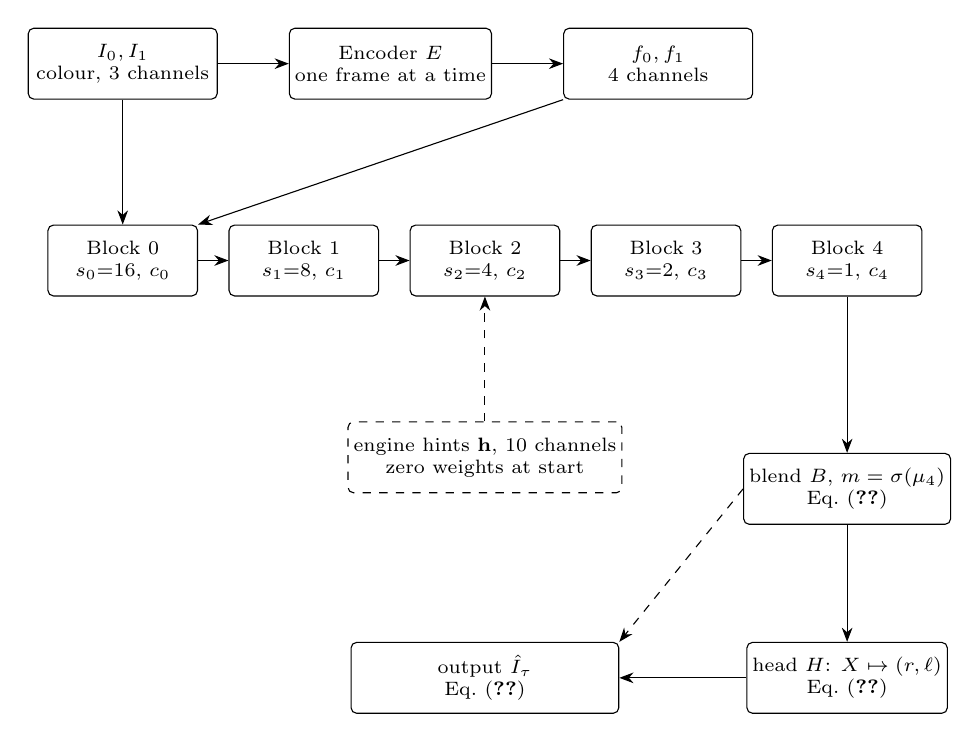
\begin{tikzpicture}[font=\scriptsize, box/.style={draw, rounded corners=2pt, align=center, minimum height=9mm, minimum width=19mm, inner sep=2pt},
  dashbox/.style={box, dashed}, arr/.style={-{Stealth[length=1.8mm]}}]
\node[box, minimum width=24mm] (in) at (0,0) {$I_0,I_1$\\colour, 3 channels};
\node[box, minimum width=24mm] (enc) at (3.4,0) {Encoder $E$\\one frame at a time};
\node[box, minimum width=24mm] (feat) at (6.8,0) {$f_0,f_1$\\4 channels};
\node[box] (b0) at (0,-2.5) {Block 0\\$s_0{=}16$, $c_0$};
\node[box] (b1) at (2.3,-2.5) {Block 1\\$s_1{=}8$, $c_1$};
\node[box] (b2) at (4.6,-2.5) {Block 2\\$s_2{=}4$, $c_2$};
\node[box] (b3) at (6.9,-2.5) {Block 3\\$s_3{=}2$, $c_3$};
\node[box] (b4) at (9.2,-2.5) {Block 4\\$s_4{=}1$, $c_4$};
\node[dashbox, minimum width=24mm] (hint) at (4.6,-5.0) {engine hints $\mathbf h$, 10 channels\\zero weights at start};
\node[box, minimum width=24mm] (blend) at (9.2,-5.4) {blend $B$, $m=\sigma(\mu_4)$\\Eq.~\eqref{eq:fgm-blend}};
\node[box, minimum width=24mm] (head) at (9.2,-7.8) {head $H$: $X\mapsto(r,\ell)$\\Eq.~\eqref{eq:fgm-head-in}};
\node[box, minimum width=34mm] (out) at (4.6,-7.8) {output $\hat I_\tau$\\Eq.~\eqref{eq:fgm-out}};
\draw[arr] (in.east) -- (enc.west);
\draw[arr] (enc.east) -- (feat.west);
\draw[arr] (in.south) -- (b0.north);
\draw[arr] (feat.south west) -- (b0.north east);
\draw[arr] (b0.east) -- (b1.west);
\draw[arr] (b1.east) -- (b2.west);
\draw[arr] (b2.east) -- (b3.west);
\draw[arr] (b3.east) -- (b4.west);
\draw[arr, dashed] (hint.north) -- (b2.south);
\draw[arr] (b4.south) -- (blend.north);
\draw[arr] (blend.south) -- (head.north);
\draw[arr] (head.west) -- (out.east);
\draw[arr, dashed] (blend.west) -- (out.north east);
\end{tikzpicture}
\caption{IFNet with the head. The encoder runs once per frame. Block $k$ takes the warped frames and features under the current flow, the previous mask and features, and $\tau$ (Eqs.~\eqref{eq:fgm-block0} and \eqref{eq:fgm-blockk}), and it outputs $\Delta_k$, $\mu_k$ and $\varphi_k$ (Eq.~\eqref{eq:fgm-blockout}). Engine hints enter every block through zero-initialised weights (\cref{sec:fgm-hints}). Block 4 gives the blend $B$, and the half-resolution head gives the residual $r$ and the UI logit, which form the output (Eqs.~\eqref{eq:fgm-head-in} and \eqref{eq:fgm-out}). The block scales and widths shown are those of the \tier{high} tier}\label{fig:fgm-ifnet}
\end{figure}

\subsection{RIFE 4.26 weights and the reproduction check}\label{sec:fgm-weights}

The weights are RIFE 4.26's archive, published in the author's Hugging Face repository. The downloader checks the SHA-256 hash of the archive and then of the \texttt{flownet.pkl} file inside it, and it loads the state dictionary with \texttt{weights\_only=True}, so the file cannot run code. The parameter names and shapes of the \tier{high} tier equal RIFE's, so every tensor is loaded by name. Where a tensor of a tier is smaller than its RIFE counterpart, the loader copies the leading slice along every dimension, the minimum of the two sizes. Where RIFE has more residual blocks than the tier, the first $n$ blocks are copied and the rest are ignored. Tensors that have no RIFE counterpart keep their initialisation, and the hint input columns keep their zero weights (\cref{sec:fgm-hints}). For the \tier{high} tier the loader reports 153 tensors copied exactly and 5 copied with a slice. The five sliced tensors are the first convolutions of the blocks, which are widened by the 10 hint channels, and no tensor is missing.

\emph{Reproduction check.} The check compares the \tier{high} tier with RIFE 4.26's own network code, the \texttt{IFNet\_HDv3} module of the archive, on the same inputs and with no engine data. RIFE's warp function is not in the archive, so the check recreates it with the grid convention of \cref{eq:fgm-warp}. The inputs are a random $8\times12$ image upsampled bicubically to $128\times192$ as $I_0$, and $I_0$ rolled by $(2,5)$ pixels as $I_1$, at $\tau=1/2$. The repository's check accepts a difference below $10^{-4}$ between the blend $B$ and RIFE's merged output in float32 on the CPU, and the agreement it measures is below $10^{-5}$. It also checks that the residual head and the hints add nothing at initialisation (\cref{sec:fgm-hints,sec:fgm-output}). The check tests the network code against RIFE's network code. It does not test the warp against RIFE's own kernel, and it does not test the delivered output of the generator, which differs from the blend (\cref{sec:fgm-output}).

\subsection{Tiers and channel-slice inheritance}\label{sec:fgm-tiers}

\Cref{tab:fgm-tiers} lists the four tiers. The \tier{high} tier has RIFE's widths, residual depth and block layout, and it is the one that starts from RIFE 4.26's network. The smaller tiers are narrower, with fewer residual blocks per block and a narrower head. Each tier is the generator of \cref{eq:fgm-task} with its own widths, residual depth, head width and flow line limit.

\begin{table}[!htbp]
\caption{Frame-generation tiers. Widths are the channel counts of blocks 0 to 4, $n$ the residual blocks per block, $c_h$ the head width, $L$ the flow line limit of \cref{eq:fgm-scale}, and GMAC the multiply-accumulates per 1080p output frame (every convolution, warps excluded), with flow at the scale the tier uses at 1080p}\label{tab:fgm-tiers}
\begin{tabular*}{\textwidth}{@{\extracolsep\fill}lllrrrr}
\toprule
Tier & Widths $c_0,\dots,c_4$ & $n$ & $c_h$ & $L$ & Params & GMAC \\
\midrule
\tier{igpu} & 64, 48, 32, 24, 16 & 3 & 12 & 576 & \Res{fg.model_tiers.igpu.params} & \Res{fg.model_tiers.igpu.gmac_per_1080p_frame} \\
\tier{low} & 96, 64, 48, 32, 16 & 4 & 16 & 576 & \Res{fg.model_tiers.low.params} & \Res{fg.model_tiers.low.gmac_per_1080p_frame} \\
\tier{mid} & 128, 96, 64, 48, 24 & 6 & 24 & 1152 & \Res{fg.model_tiers.mid.params} & \Res{fg.model_tiers.mid.gmac_per_1080p_frame} \\
\tier{high} & 192, 128, 96, 64, 32 & 8 & 32 & 1152 & \Res{fg.model_tiers.high.params} & \Res{fg.model_tiers.high.gmac_per_1080p_frame} \\
\bottomrule
\end{tabular*}
\end{table}

\emph{Channel-slice inheritance.} A smaller tier starts from RIFE's weights through the copy rule of \cref{sec:fgm-weights}. The narrower tensors take the leading channels of RIFE's tensor along each channel dimension, so the output channels of a block and the input channels of the next layer keep the same ordering. For the \tier{igpu} tier the loader reports 13 tensors with exact shapes and 70 sliced, for the \tier{low} tier 13 and 85, and for the \tier{mid} tier 13 and 115, with no missing tensor. The head has no RIFE counterpart, so it starts from its initialisation in every tier. The inheritance is a heuristic. Nothing forces RIFE's leading channels to be the best subset for a narrower network, and the ablation without inheritance (\cref{sec:fgm-ablate}) is the test of how much it matters.

\subsection{Flow-resolution caps and their cost}\label{sec:fgm-caps}

Estimating flow at full resolution is the most expensive part of the network, so every tier caps the number of image lines at which it estimates flow. A frame of height $H$ lines is halved until it fits under the tier's limit $L$, as RIFE's own scale argument allows:
\begin{equation}
s(H)=2^{-j^\ast},\qquad j^\ast=\min\big\{\,j\in\mathbb N_0:\,H\,2^{-j}\le L\,\big\},\label{eq:fgm-scale}
\end{equation}
with $L=576$ lines for the \tier{igpu} and \tier{low} tiers and $L=1152$ lines for the \tier{mid} and \tier{high} tiers. At 1080 lines the \tier{igpu} and \tier{low} tiers therefore estimate flow at $s=1/2$ (540 lines), and the \tier{mid} and \tier{high} tiers at $s=1$. The 256-pixel training crops and video up to 576 lines keep full-resolution flow in every tier. The frames are downsampled by $s$ before the encoder and the blocks, the flow hints are multiplied by $s$, and the flows that come out are upsampled and multiplied by $1/s$ to return to pixels. The head, the warps and the output stay at full resolution.

The convolution cost of the encoder and the blocks scales with the pixel count of the frames they see, so it scales with $s^2$. The head does not change. \Cref{tab:fgm-cap} gives the consequence at 1080p, counted with the same hooks as \cref{tab:fgm-tiers}. The cap removes more than half of the flow-path cost of the \tier{igpu} and \tier{low} tiers. For the \tier{low} tier the head is about a third of the capped cost, so the head matters most for the smallest tiers.

\begin{table}[!htbp]
\caption{Cost per 1080p generated frame of the tiers with the flow cap of \cref{eq:fgm-scale} and with full-resolution flow (GMAC, warps excluded). The encoder column counts both real frames, as the repository's tier table does, so one encoder pass is half of it. The head is the residual head of \cref{sec:fgm-output}}\label{tab:fgm-cap}
\begin{tabular*}{\textwidth}{@{\extracolsep\fill}lrrrrr}
\toprule
Tier & Flow scale & Capped total & Full-flow total & Encoder (two frames) & Head \\
\midrule
\tier{igpu} & \Res{fg.model_tiers.igpu.flow_scale_1080p} & \Res{fg.model_tiers.igpu.gmac_per_1080p_frame} & 20.4 & \Res{fg.model_tiers.igpu.gmac_per_frame_encoder} & 2.9 \\
\tier{low} & \Res{fg.model_tiers.low.flow_scale_1080p} & \Res{fg.model_tiers.low.gmac_per_1080p_frame} & 25.5 & \Res{fg.model_tiers.low.gmac_per_frame_encoder} & 4.5 \\
\tier{mid} & \Res{fg.model_tiers.mid.flow_scale_1080p} & \Res{fg.model_tiers.mid.gmac_per_1080p_frame} & 44.3 & \Res{fg.model_tiers.mid.gmac_per_frame_encoder} & 8.5 \\
\tier{high} & \Res{fg.model_tiers.high.flow_scale_1080p} & \Res{fg.model_tiers.high.gmac_per_1080p_frame} & 76.7 & \Res{fg.model_tiers.high.gmac_per_frame_encoder} & 13.8 \\
\bottomrule
\end{tabular*}
\end{table}

\subsection{Engine hints and their zero initialisation}\label{sec:fgm-hints}

When an engine provides data, the generator receives them as extra input channels of every IFNet block. \Cref{tab:fgm-hints} lists the ten channels in the order of the code. The signal channels are multiplied by their availability, so an absent signal contributes zero, and the flags tell the network which case it is in.

\emph{Motion priors.} If a point moves with constant velocity between $I_0$ and $I_1$, its displacement from $I_1$ to $I_0$ is $M_1$, and at time $\tau$ its displacement to $I_0$ is $\tau M_1$ and to $I_1$ is $(\tau-1)M_1$. The priors are exact only for linear motion, so the network has to learn when to trust them. The zero initialisation below lets it start from a working point.

\emph{Camera-only flow and late latching.} The camera flow $C$ is the displacement that the camera motion alone induces on the static background, from the target pixel to $I_1$. Let $A_t$ be the background affine map from screen to texture at time $t$ (\cref{sec:data-synth}), with normalised coordinates $x\in[-1,1]^2$. Then
\begin{equation}
C(x)=\tfrac{P}{2}\big(A_1^{-1}(A_\tau(x))-x\big),
\end{equation}
where $P$ is the frame size in pixels, so that $P/2$ converts normalised displacements to pixels for a $P\times P$ frame. Object motion is absent from $C$. At display time an engine knows the camera pose of the frame it is about to show, so the pose can be latched just before generation and supplied as this prior. In the synthetic training the prior uses the exact background trajectory at $\tau$. For real video the camera availability is zero, so the prior is never present.

\emph{Depth.} The depth channel is the inverse depth of $I_1$ normalised by its median, $d_1=1/(1+d/\operatorname{median}(d))$, so that a pixel at the median depth has the value one half. It is defined only for the synthetic renderer, where the depth is exact.

\emph{Availability.} Each availability flag is set per sample, and the signal channels are multiplied by the flags. Withholding a signal in training is therefore the same as an engine that does not provide it. The withholding rates are in \cref{tab:fgm-probs}.

\begin{table}[!htbp]
\caption{Sampling probabilities of the frame-generation training data, with the configuration names used in the saved files, or the constant in the code where no configuration name exists}\label{tab:fgm-probs}
{\footnotesize\begin{tabular*}{\textwidth}{@{\extracolsep\fill}lrl}
\toprule
Quantity & Value & Configuration or constant \\
\midrule
Real share of each GPU batch & \Res{fg.config.cfg.p_real} (19 of 48) & \texttt{p\_real} \\
Extrapolation, both sample kinds & \Res{fg.config.cfg.p_extrap} & \texttt{p\_extrap} \\
Random $\tau$ for synthetic interpolation & \Res{fg.config.cfg.p_tau} & \texttt{p\_tau}, $\tau\sim U[0.15,0.85]$ \\
Multi-frame share of real interpolation & \Res{fg.config.cfg.p_mfg} & \texttt{p\_mfg} \\
Camera reversal & \Res{fg.config.cfg.p_flip} & \texttt{p\_flip} \\
Scene cut & \Res{fg.config.cfg.p_cut} & \texttt{p\_cut} \\
UI overlay & \Res{fg.config.cfg.p_ui} & \texttt{p\_ui} \\
Menu, given a UI overlay & \Res{fg.config.cfg.p_menu} & \texttt{p\_menu} \\
Withhold motion vector (synthetic) & \Res{fg.config.cfg.p_drop_mv} & \texttt{p\_drop\_mv} \\
Withhold motion vector (real) & \Res{fg.config.cfg.p_drop_mv_real} & \texttt{p\_drop\_mv\_real} \\
Withhold depth (synthetic) & 0.30 & default argument in \texttt{set\_availability} \\
Withhold camera prior (extrapolation) & 0.20 & constant in \texttt{set\_availability} \\
UI slot filled / tile changed at $t=1$ & 0.70 / 0.30 & \texttt{ui\_layer} \\
\bottomrule
\end{tabular*}}
\end{table}

\paragraph{Zero-initialisation argument.} Let $W^{\mathbf h}_k$ be the weights of the first convolution of block $k$ that multiply the hint channels, and let every other weight of the \tier{high} tier equal RIFE's. The claim is that with $W^{\mathbf h}_k=0$ for every $k$, the blend $B$ does not depend on $\mathbf h$ and equals RIFE 4.26's blend. The argument is by induction over the blocks. Block 0 receives the same input as in RIFE, so its first convolution computes $z=W_x*x+W^{\mathbf h}_0*\mathbf h+b$ with $W^{\mathbf h}_0=0$, which equals RIFE's pre-activation $W_x*x+b$. The later layers of the block see only $z$, so the block outputs $(\Delta_0,\mu_0,\varphi_0)$ equal RIFE's. The induction step is the same for block $k$, because the warps and features that enter block $k$ are functions of the earlier outputs only. The blend of \cref{eq:fgm-blend} is then RIFE's blend. The head adds nothing at initialisation, because its last layer has zero weights and bias $(0,0,0,-4)$ (\cref{sec:fgm-output}). The gradient with respect to the hint columns is $\partial L/\partial W^{\mathbf h}_k=\sum_p \delta_k(p)\,\mathbf h(p)^{\top}$, summed over the sampled positions $p$, where $\delta_k$ is the gradient at the first-layer output. This is not zero when the hints are non-zero and the loss is sensitive to block $k$, so the hint columns leave zero at the first update. The fresh model therefore reproduces RIFE's blend, and then learns from the engine data.

\subsection{Head, UI weight and output}\label{sec:fgm-output}

The head turns the warped frames into a residual colour and a UI logit. Its input is the full-resolution stack of the two real frames, the two warps under the final flow, the blend weight and the last features:
\begin{equation}
X=\big[I_0,\,I_1,\,\mathcal W(I_0,F_4^0),\,\mathcal W(I_1,F_4^1),\,m,\,\varphi_4\big]\qquad(21\text{ channels}).\label{eq:fgm-head-in}
\end{equation}
A stride-2 $3\times3$ convolution with $c_h$ channels and LeakyReLU, two residual blocks at half resolution with the design of \cref{sec:fgm-ifnet}, and a $4\times4$ transposed convolution with stride 2 give four output channels, $(r,\ell)=H(X)$. Here $r$ is the residual colour and $\ell$ the UI logit. The head starts with a zero transposed-convolution weight and bias $(0,0,0,-4)$, so $r=0$ and $\ell=-4$ at initialisation, and the UI weight $u=\sigma(\ell)$ is about $0.018$. The output is
\begin{equation}
\hat I_\tau=u\odot I_1+(1-u)\odot\big(B+r\big),\qquad u=\sigma(\ell),\label{eq:fgm-out}
\end{equation}
with the blend $B$ of \cref{eq:fgm-blend}. This is \cref{M-eq:fg} of the article.

The UI weight is a soft mask in $[0,1]$, not a hard classification. Training pushes $u$ towards one on HUD, subtitle and menu pixels, where the UI mask of \cref{eq:fgm-ui-bce} is one, and towards zero elsewhere, so that those pixels come from the newest real frame $I_1$. The starting value means that a fresh model already mixes a small fraction of $I_1$ into every pixel. The delivered output of a fresh model therefore differs from the blend by $u\odot(I_1-B)$, which is small but not zero. This is why the reproduction check of \cref{sec:fgm-weights} compares the blend and not the output.

Evaluation clamps the output to $[0,1]$ before computing metrics. Training does not clamp, so the loss sees the unclamped output.

\emph{UI layer compositing.} When an engine renders the HUD separately from the scene, it can supply HUD-less real frames and the UI layer for the newest state, as premultiplied colour $c$ and alpha $\alpha$. The generator then runs on the HUD-less frames, and the displayed frame is $\hat I_\tau(1-\alpha)+c$. In the design this is applied to every displayed frame of the layer's sequence. The evaluation applies it to the generated frame only (\cref{sec:fgm-test}).

\subsection{Per-frame encoder reuse}\label{sec:fgm-encoder}

The encoder of \cref{eq:fgm-enc} depends on one frame, so a running sequence can encode each real frame once and reuse its features. The IFNet forward pass takes optional precomputed features for this, but no caller in the repository passes them. Training, evaluation and the exported graph all encode both frames (\cref{sec:fgm-export}).

The cost accounting follows from this. The encoder column of \cref{tab:fgm-cap} counts two frames, so one pass per real frame is half the column. With one generated frame per real frame, reuse replaces two encoder passes per generated frame by one.

\subsection{Scene-cut gate}\label{sec:fgm-cut}

\UnderRevision{} The gate decides when the generator should not generate. When two real frames look as if a scene cut lies between them, it outputs the newest real frame $I_1$ instead of $\hat I_\tau$. The repository marks this stage as a known weakness. Its thresholds are calibrated on synthetic adjacent pairs only, so the calibration does not cover real content or wider frame gaps.

The score combines a colour-distribution distance, which needs no motion, with a motion-compensated difference, which is used when $M_1$ is available. Let $Y(x)=(16+65.481R(x)+128.553G(x)+24.966B(x))/255$ be the limited-range luma of an RGB pixel with values in $[0,1]$, and let $h(I)\in\mathbb R^{32}$ be the fraction of pixels whose luma falls in each of 32 equal bins of $[0,1]$. The histogram distance and the motion-compensated difference are
\begin{align}
d_{\rm h}(I_0,I_1)&=\tfrac12\big\|h(I_0)-h(I_1)\big\|_1\in[0,1],\label{eq:fgm-hist}\\
d_{\rm m}(I_0,I_1,M_1)&=\frac{1}{3HW}\sum_{x,c}\big|I_1(x,c)-\mathcal W(I_0,M_1)(x,c)\big|.\label{eq:fgm-hist-m}
\end{align}
The two scores are
\begin{equation}
S_{\rm mv}=d_{\rm h}+2\,d_{\rm m},\qquad S_0=d_{\rm h},\label{eq:fgm-score}
\end{equation}
and the gate is
\begin{equation}
g=\begin{cases}\mathbf 1[S_{\rm mv}>\theta_{\rm mv}] & \text{if }a_{\rm mv}=1,\\ \mathbf 1[S_0>\theta_0] & \text{otherwise,}\end{cases}\label{eq:fgm-gate}
\end{equation}
where $\mathbf 1[\cdot]$ is one when its condition holds and zero otherwise. Without motion vectors the histogram distance alone is used, because a raw frame difference would read ordinary fast motion as a cut. The gate lives in the evaluation code, and it is not part of the exported graph.

\emph{Calibration.} Each threshold is set separately on synthetic pairs, so that continuous motion is a false alarm on about one pair in a hundred.
\begin{enumerate}
\item Draw four batches of up to 64 validation stills. For each batch, generate interpolation pairs at $\tau=1/2$ with motion from all four speed classes, no camera reversal and no UI, and with a cut probability of one half. Each pair is labelled cut or continuous. This gives 256 pairs, about half of them cuts.
\item Compute $S_{\rm mv}$ with the exact motion vector and $S_0$ for every pair.
\item For each score, sort the scores of the continuous pairs in ascending order and take the element at 0-based index $\lfloor0.99(n-1)\rfloor$, where $n$ is the number of continuous pairs. This element is the threshold $\theta$.
\item Report the detection rate, which is the share of cut pairs whose score exceeds $\theta$.
\end{enumerate}
The calibrated values are part of the results (\cref{sec:fgr}). When the gate fires, the output is the newest real frame,
\begin{equation}
\hat I_\tau\quad\leftarrow\quad I_1\qquad\text{if } g=1.\label{eq:fgm-gated}
\end{equation}

\subsection{Latency model and pacing}\label{sec:fgm-pacing}

\UnderRevision{} The latency numbers are timed on one data-centre GPU in eager PyTorch, and the pacing model is a simulation with assumed scheduling. The latency terms are those of \cref{sec:bg-latency}. The repository marks in-engine latency on target hardware as not measured. The model therefore answers what frame generation does to the displayed rate and to two latencies, under the stated assumptions.

The model is a discrete-event simulation of a GPU-bound loop with just-in-time CPU scheduling, in which the CPU starts each frame's work so that the GPU never queues frames, on a variable-refresh display. Its parameters are in \cref{tab:fgm-pacing}. The modes are \emph{native} (no generation), \emph{interpolation} (a generated frame between two real frames, with the newer real frame held), \emph{extrapolation} (a generated frame after the newest real frame, with nothing held) and \emph{extrapolation with late latching} (extrapolation whose camera is sampled just before generation).

\begin{table}[!htbp]
\caption{Parameters of the pacing model, as set in the simulation code and the notebook. The generation time $T_{\rm gen}$ is the measured one-generated-frame time of the \tier{low} tier at 1080p (\cref{sec:fgr}). The temporal super-resolution time $T_{\rm sr}$ is zero, because this pacing run has no such stage}\label{tab:fgm-pacing}
\begin{tabular*}{\textwidth}{@{\extracolsep\fill}lll}
\toprule
Symbol & Value & Meaning \\
\midrule
$R_0$ & 33.3, 25.0, 16.7\,ms & base render time per real frame (30, 40 and 60 fps renders) \\
$C_{\rm cpu}$ & 4.0\,ms & CPU time per frame before rendering starts \\
$c_v$ & 0.08 & log-normal spread of the render time \\
$T_{\rm pres}$ & 1.0\,ms & present time \\
$T_{\rm sr}$ & 0 & temporal super-resolution time \\
$T_{\rm gen}$ & measured & frame generation time per generated frame \\
$N$ & 2000 & simulated real frames per run \\
seed & 0 & random seed of the render times \\
\bottomrule
\end{tabular*}
\end{table}

The simulation runs as follows.
\begin{enumerate}
\item For each real frame $j=1,\dots,N$, draw the render time $R_j=R_0\exp(c_v z_j)$, where $z_j$ is standard normal.
\item Set the GPU time $g_j=R_j+T_{\rm sr}+T_{\rm gen}\,\mathbf 1[\text{mode}\neq\text{native}]$ and the frame period $\pi_j=\max(C_{\rm cpu},g_j)$.
\item Let $t_j$ be the time of the input sample, which is the current simulation time.
\item Set the time at which the rendered real frame is ready, $a_j=t_j+C_{\rm cpu}+R_j+T_{\rm sr}$.
\item In the \emph{native} mode, display the real frame at $p^{\rm r}_j=a_j+T_{\rm pres}$.
\item In the \emph{interpolation} mode, display the generated frame at $p^{\rm g}_j=a_j+T_{\rm gen}+T_{\rm pres}$, and hold the real frame until $p^{\rm r}_j=p^{\rm g}_j+\pi_j/2$.
\item In the \emph{extrapolation} mode, display the real frame at $p^{\rm r}_j=a_j+T_{\rm pres}$, and the generated frame at $p^{\rm g}_j=p^{\rm r}_j+\pi_j/2$.
\item In the \emph{extrapolation with late latching} mode, proceed as in step 7, and sample the camera of the generated frame at $t^{\rm cam}_j=p^{\rm g}_j-T_{\rm gen}-T_{\rm pres}$, the moment generation starts.
\item Record the displayed frames and the latency samples below, and advance the simulation time by $t\leftarrow t+\pi_j$.
\end{enumerate}
The rates are computed on the displayed times after the first tenth of the displayed sequence, so that start-up does not count. With $\Delta_i$ the gaps between consecutive displayed times, the displayed frame rate and the gap variation are $\mathrm{fps}=1000/\overline\Delta$ and $\mathrm{CV}=\operatorname{sd}(\Delta)/\overline\Delta$, in milliseconds for $\Delta$.

Three latencies are reported. The game input latency is the time from an input sample to the display of the real frame that reflects it, averaged over the real frames of the run,
\begin{equation}
L_{\rm game}=\operatorname{mean}_j\big(p^{\rm r}_j-t_j\big).\label{eq:fgm-lat-game}
\end{equation}
The camera latency is the same kind of time, measured to each displayed frame that counts as reflecting the camera. In the code a native frame counts with its real display. An interpolated frame counts with its generated display only, on the assumption that the generated frame already moves half way toward the camera of the newer frame. An extrapolated frame counts with both its real and its generated display, and with late latching the generated display is measured from $t^{\rm cam}_j$:
\begin{equation}
L_{\rm cam}=\begin{cases}\operatorname{mean}_j\big(p^{\rm r}_j-t_j\big) & \text{native},\\[2pt] \operatorname{mean}_j\big(p^{\rm g}_j-t_j\big) & \text{interpolation},\\[2pt] \tfrac12\Big(\operatorname{mean}_j\big(p^{\rm r}_j-t_j\big)+\operatorname{mean}_j\big(p^{\rm g}_j-t_j\big)\Big) & \text{extrapolation},\\[2pt] \tfrac12\Big(\operatorname{mean}_j\big(p^{\rm r}_j-t_j\big)+\operatorname{mean}_j\big(p^{\rm g}_j-t^{\rm cam}_j\big)\Big) & \text{late latching.}\end{cases}\label{eq:fgm-lat-cam}
\end{equation}
The content age averages the time from the input sample to every displayed frame, real or generated,
\begin{equation}
A=\operatorname{mean}_p\big(p-t\big)\quad\text{over all displayed frames }p.\label{eq:fgm-lat-age}
\end{equation}
Each latency is also reported at its 95th percentile over the samples.

The arithmetic estimate of a network's time at a sustained throughput $F$ in TFLOPS, is $T_{\rm est}=2G/F$ milliseconds, for a frame that costs $G$ GMAC, because one multiply-accumulate is two floating-point operations. The repository uses $F=4$ TFLOPS for an assumed integrated GPU. The estimate scales the GMAC with pixel count, so at 1440p it ignores the flow cap of \cref{eq:fgm-scale}.

\begin{figure}[!htbp]
\centering
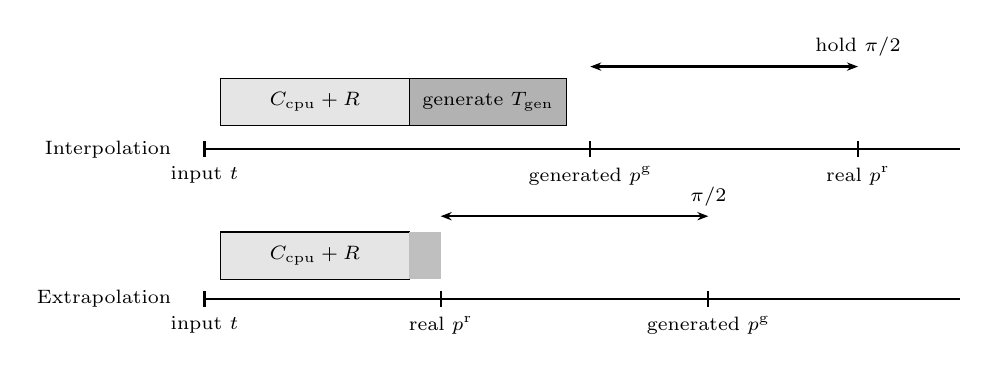
\begin{tikzpicture}[font=\scriptsize, x=1cm, y=1cm,
  tick/.style={thick},
  lab/.style={font=\scriptsize, align=center},
  bar/.style={draw, minimum height=6mm, inner sep=1pt}]
\node[anchor=east, lab] at (-0.3,1.9) {Interpolation};
\draw[thick] (0,1.9) -- (9.6,1.9);
\node[bar, fill=black!10, minimum width=2.4cm] at (1.4,2.5) {$C_{\rm cpu}+R$};
\node[bar, fill=black!30, minimum width=2.0cm] at (3.6,2.5) {generate $T_{\rm gen}$};
\draw[tick] (0,1.8) -- (0,2.0);
\node[lab, below] at (0,1.8) {input $t$};
\draw[tick] (4.9,1.8) -- (4.9,2.0);
\node[lab, below] at (4.9,1.8) {generated $p^{\rm g}$};
\draw[tick] (8.3,1.8) -- (8.3,2.0);
\node[lab, below] at (8.3,1.8) {real $p^{\rm r}$};
\draw[{Stealth[length=1.4mm]}-{Stealth[length=1.4mm]}, thick] (4.9,2.95) -- (8.3,2.95) node[above, lab] {hold $\pi/2$};
\node[anchor=east, lab] at (-0.3,0.0) {Extrapolation};
\draw[thick] (0,0.0) -- (9.6,0.0);
\node[bar, fill=black!10, minimum width=2.4cm] at (1.4,0.55) {$C_{\rm cpu}+R$};
\fill[black!25] (2.6,0.25) rectangle (3.0,0.85);
\draw[tick] (0,-0.1) -- (0,0.1);
\node[lab, below] at (0,-0.1) {input $t$};
\draw[tick] (3.0,-0.1) -- (3.0,0.1);
\node[lab, below] at (3.0,-0.1) {real $p^{\rm r}$};
\draw[tick] (6.4,-0.1) -- (6.4,0.1);
\node[lab, below] at (6.4,-0.1) {generated $p^{\rm g}$};
\draw[{Stealth[length=1.4mm]}-{Stealth[length=1.4mm]}, thick] (3.0,1.05) -- (6.4,1.05) node[above, lab] {$\pi/2$};
\end{tikzpicture}
\caption{Timeline of one input sample in the two generation modes, schematic and not to scale. In interpolation the generated frame needs the newest real frame, and the real frame is held for half a period, so it is shown after the generated frame. In extrapolation the real frame is shown as soon as it is rendered, and the generated frame follows half a period later, with the generation time $T_{\rm gen}$ inside that period. The grey bar at $T_{\rm pres}$ in the extrapolation row is the present time. The labels are the symbols of \cref{tab:fgm-pacing}}\label{fig:fgm-timeline}
\end{figure}

\cref{fig:fgm-timeline} shows the two modes. Interpolation adds $T_{\rm gen}$ to the time of the generated frame and delays the real frame by half a period. Extrapolation adds no delay to the real frame and adds half a period to the generated frame, which is shown after the real frame.

\subsection{Training samples}\label{sec:fgm-samples}

In the main stages each of the two GPUs takes its own batch of 48 samples per step, under distributed data parallel training. A batch holds 19 real quads and 29 synthetic samples, since the real share \Res{fg.config.cfg.p_real} of 48 rounds to 19, drawn at random without replacement from the caches. Still crops are $512\times512$ pixels cut from the textures of \cref{sec:data-synth}, and quads are four frames of $256\times256$ pixels from the sequence sources of \cref{sec:data}, both after the random downscale of \cref{sec:data}. The cache sizes are in \cref{sec:fgr}.

\paragraph{Synthetic samples.} Each synthetic sample is one scene of the renderer of \cref{sec:data-synth}, rendered at $256\times256$ pixels with four anti-aliasing samples per pixel for $I_0$, $I_1$ and the target. The background is one still. The foreground is the still of the neighbouring sample in the batch, visible through a procedural alpha mask in 85 percent of samples, and a flat colour in 25 percent of samples. The construction of one sample is as follows.
\begin{enumerate}
\item Draw the camera reversal with probability \Res{fg.config.cfg.p_flip}. A reversal reverses the camera velocity after $t=1$.
\item Draw extrapolation with probability \Res{fg.config.cfg.p_extrap}. If it is extrapolation, set $\tau=1.5$. Otherwise set $\tau=1/2$, or with probability \Res{fg.config.cfg.p_tau} draw $\tau$ uniformly from $[0.15,0.85]$.
\item Render $I_0$ at $t=0$, $I_1$ at $t=1$ and the target at $t=\tau$.
\item Compute the exact motion vector $M_1$, which is the flow from $I_1$ to $I_0$, the exact flows $F_{\tau\to0}$ and $F_{\tau\to1}$ with their validity masks (visible and inside the view), the camera flow $C$ and the inverse depth $d_1$.
\item Draw a scene cut with probability \Res{fg.config.cfg.p_cut}. A cut replaces $I_1$, $M_1$ and $d_1$ by those of the neighbouring sample, sets the target to the replaced $I_1$, and sets the validity masks to zero.
\item Draw UI overlays with probability \Res{fg.config.cfg.p_ui}. Four UI slots are each filled with probability 0.7 by a tile from a bank of 256 text, bar and crosshair tiles of $160\times28$ pixels, and 30 percent of the filled slots change their tile at $t=1$. A full-screen menu panel of alpha 0.6 and colour 0.05 is drawn with probability \Res{fg.config.cfg.p_menu} given a UI overlay, which is 1.5 percent of all samples. The tiles are alpha-composited into $I_0$ with the state at $t=0$, into $I_1$ with the state at $t=1$, and into the target with the state at $t=1$. The UI mask is the maximum of the two alphas.
\item Withhold the signals according to \cref{tab:fgm-probs}, and set the camera availability to zero for every interpolation sample.
\end{enumerate}

\paragraph{Real quads.} Each real sample is a window of four consecutive frames from one of the sequence sources of \cref{sec:data}, decoded and cut to $256\times256$ pixels. The window is flipped horizontally and vertically with probability one half each, and its flow fields are flipped with it, with the vector components negated along each flipped axis. The sample then takes one of three forms.
\begin{enumerate}
\item With probability \Res{fg.config.cfg.p_extrap}, extrapolation: $I_0=k$, $I_1=k+2$ and target $k+3$, at $\tau=1.5$.
\item Otherwise, with probability \Res{fg.config.cfg.p_mfg}, multi-frame generation: $I_0=k$, $I_1=k+3$, and the target is $k+1$ or $k+2$ with equal probability, at $\tau=1/3$ or $2/3$.
\item Otherwise interpolation: $I_0=k$, $I_1=k+2$ and target $k+1$, at $\tau=1/2$.
\end{enumerate}
The flows come from the RAFT optical-flow network \cite{teed2020raft}, in the small variant that torchvision ships with its weights. The cache computes four flows per quad, $k+2\to k$, $k+1\to k$, $k+1\to k+2$ and $k+3\to k+2$, at the $256\times256$ crop size, and stores them at half resolution, in pixels of the full grid, by two-by-two average pooling. Every quad carries these four flows, including the TartanAir and Sintel quads that have exact flows in the frame decoder, because the quad cache does not use those flows. The motion vector $M_1$ is the flow $k+2\to k$. The flows $F_{\tau\to0}$ and $F_{\tau\to1}$ are $k+1\to k$ and $k+1\to k+2$ for interpolation, and $k+3\to k+2$ for extrapolation. An extrapolated sample has no label from the target to $I_0$, so its $F_{\tau\to0}$ validity is zero. A multi-frame sample has no flow label, so its $M_1$ and both flow validities are zero. A real sample has no depth and no camera prior, so its depth and camera availabilities are zero. Every pixel of a real flow is valid, because the cache computes no validity mask.

\paragraph{Availability and the plain-video case.} \Cref{tab:fgm-probs} gives the withholding rates. Synthetic samples withhold the motion vector with probability \Res{fg.config.cfg.p_drop_mv} and the depth with probability 0.3, and they keep the camera prior with probability 0.8 on extrapolation samples only. Real samples withhold the motion vector with probability \Res{fg.config.cfg.p_drop_mv_real} when a flow label exists, and they never have depth or a camera prior. The validation batches are fixed, with \Res{fg.config.cfg.val_bs} stills and \Res{fg.config.cfg.val_bs} quads in each of \Res{fg.config.cfg.val_batches} batches, drawn with a seed of 54321. Each is evaluated twice, once with its availabilities and once with all of them set to zero, which is plain video.

\subsection{Training objective}\label{sec:fgm-loss}

The objective is a weighted sum of six terms, with a unit weight on the first,
\begin{equation}
\mathcal L=\mathcal L_{\rm pix}+0.5\,\mathcal L_{\rm cen}+0.1\,\mathcal L_{\rm lp}+0.01\,\mathcal L_{\rm flow}+0.2\,\mathcal L_{\rm ui}+0.5\,\mathcal L_{\rm kd},\label{eq:fgm-total}
\end{equation}
where each term is a mean over the batch. \Cref{tab:fgm-loss} gives the definitions, and the paragraphs below give the formulas.

\begin{table}[!htbp]
\caption{Training losses of the frame generator, with weights and the samples to which each term applies}\label{tab:fgm-loss}
\begin{tabular*}{\textwidth}{@{\extracolsep\fill}lp{0.42\textwidth}rp{0.30\textwidth}}
\toprule
Term & Quantity & Weight & Applies to \\
\midrule
$\mathcal L_{\rm pix}$ & Charbonnier penalty, $\varepsilon=10^{-3}$ & 1 & every sample \\
$\mathcal L_{\rm cen}$ & soft census distance, $7\times7$ window & \Res{fg.config.cfg.w_census} & every sample \\
$\mathcal L_{\rm lp}$ & LPIPS with AlexNet, on the clipped output & \Res{fg.config.cfg.w_lpips} & every sample, when the package loads \\
$\mathcal L_{\rm flow}$ & flow L1 on valid pixels, weight 1 (synthetic) or 1/4 (real) & \Res{fg.config.cfg.w_flow} & every sample with flow labels \\
$\mathcal L_{\rm ui}$ & binary cross-entropy on the UI mask, positive weight 4 & \Res{fg.config.cfg.w_ui} & every sample \\
$\mathcal L_{\rm kd}$ & distillation from the \tier{high} teacher & \Res{fg.config.cfg.w_distill} & students only \\
\bottomrule
\end{tabular*}
\end{table}

\emph{Charbonnier.} With the target $I_\tau$ and the output $\hat I_\tau$, $\mathcal L_{\rm pix}=\operatorname{mean}\sqrt{(\hat I_\tau-I_\tau)^2+\varepsilon^2}$, where the mean runs over every colour value. This is a smooth form of the L1 penalty. It is a smooth edge-preserving potential of the Charbonnier family \cite{charbonnier1997deterministic}.

\emph{Census.} For a grey image $g=0.299R+0.587G+0.114B$, the census vector at pixel $x$ has one soft-ternary entry per offset $\delta$ in the $7\times7$ window $D$, which has 49 offsets including zero,
\begin{equation}
c(x,\delta)=\frac{g(x+\delta)-g(x)}{\sqrt{0.81+\big(g(x+\delta)-g(x)\big)^2}}.\label{eq:fgm-census}
\end{equation}
The census distance at a pixel is $\rho(x)=\operatorname{mean}_{\delta\in D}\,d/(0.1+d)$, with $d=\big(c_{\hat I}(x,\delta)-c_{I}(x,\delta)\big)^2$. The loss $\mathcal L_{\rm cen}$ is the mean of $\rho$ over the image with a border of three pixels removed on each side. Census distances are insensitive to brightness offsets, the property for which the census loss was introduced for unsupervised flow \cite{meister2018unflow}. The soft-ternary normalisation and the robust distance are the repository's own choices.

\emph{LPIPS.} $\mathcal L_{\rm lp}$ is the LPIPS distance with the AlexNet network and version 0.1 of its calibration weights \cite{zhang2018lpips}, applied to the output clipped to $[0,1]$ and to the target, and averaged over the batch. The weight is zero when the package does not load, and the saved configuration records that.

\emph{Flow.} The flow term is the weighted L1 error of both flows over the valid pixels,
\begin{align}
\mathcal L_{\rm flow}&=\frac{\sum_x\sum_{c}\big|\hat F_{0,c}(x)-F_{0,c}(x)\big|\,v_0(x)}{2\sum_x v_0(x)+1}\nonumber\\
&\quad+\frac{\sum_x\sum_{c}\big|\hat F_{1,c}(x)-F_{1,c}(x)\big|\,v_1(x)}{2\sum_x v_1(x)+1},\label{eq:fgm-flow}
\end{align}
where $c\in\{x,y\}$ runs over the two flow components.
where $v_i=w\,\mathrm{valid}_i$ with $w=1$ for synthetic samples and $w=1/4$ for real samples. The denominator counts the valid pixels and not their weights, so a real sample contributes a quarter of the error of a synthetic one at the same pixel error.

\emph{UI.} With $y(x)=\mathbf 1[\mathrm{ui}(x)>0.5]$ for the UI mask $\mathrm{ui}=\max(\alpha_0,\alpha_1)$ of \cref{sec:fgm-samples},
\begin{equation}
\mathcal L_{\rm ui}=-\operatorname{mean}\Big[4\,y\log\sigma(\ell)+(1-y)\log\big(1-\sigma(\ell)\big)\Big],\label{eq:fgm-ui-bce}
\end{equation}
which is the binary cross-entropy on the UI logit $\ell$, with the positive term weighted by four to up-weight the rarer UI pixels.

\emph{Distillation.} When a teacher checkpoint is given, the teacher is the \tier{high} tier with the same inputs and availabilities, run without gradients. With $\hat I^{\rm T}$ and $\hat F^{\rm T}_i$ the teacher output and flows,
\begin{equation}
\mathcal L_{\rm kd}=\operatorname{mean}\big|\hat I_\tau-\hat I^{\rm T}\big|+0.01\Big(\operatorname{mean}\big|\hat F_0-\hat F^{\rm T}_0\big|+\operatorname{mean}\big|\hat F_1-\hat F^{\rm T}_1\big|\Big).\label{eq:fgm-kd}
\end{equation}
Training a student to match a teacher's outputs in this way is distillation \cite{gou2021knowledge}. The 0.01 weight on the flows is a constant of the code, not a configuration value.

\subsection{Optimisation and schedule}\label{sec:fgm-schedule}

The optimiser is AdamW \cite{loshchilov2019adamw} with betas $(0.9,0.99)$ and weight decay \Res{fg.config.cfg.weight_decay} on all parameters. The gradient norm is clipped to \Res{fg.config.cfg.grad_clip} after unscaling. The forward pass runs under fp16 autocast with dynamic loss scaling, and the losses are computed in float32 \cite{micikevicius2018mixed}. The learning rate follows the fraction $p=t/T$ of the wall-clock budget $T$ already used. It rises linearly over the first \Res{fg.config.cfg.warmup_frac} of the budget and then decays with a cosine to a floor of $\mathrm{lr}_{\min}=10^{-6}$:
\begin{equation}
\mathrm{lr}(p)=\begin{cases}\mathrm{lr}_0\,\max(p/0.03,\,0.01) & p<0.03,\\ \mathrm{lr}_{\min}+\tfrac12(\mathrm{lr}_0-\mathrm{lr}_{\min})\big(1+\cos\pi q\big) & p\geq0.03,\end{cases}\qquad q=\frac{p-0.03}{0.97}.\label{eq:fgm-lr}
\end{equation}
A moving average of the weights, the exponential moving average (EMA), is updated after every step on the rank-0 model with decay $d_s=\min(0.999,(1+s)/(10+s))$ at step $s$, so the decay starts near zero and reaches \Res{fg.config.cfg.ema_decay}. Validation runs every $\min(8\,\mathrm{min},\max(T/6,60\,\mathrm{s}))$ and at the end of the budget. Each validation saves the latest weights, and the best weights by the selection metric, which is the mean of the PSNR with and without engine data (\cref{sec:fgm-test}). The run stops with an error after 200 consecutive steps with a non-finite loss. If a run exhausts GPU memory, it is retried once with half the batch for the rest of its budget.

Training follows two stages, listed in \cref{tab:fgm-runs}. First the \tier{high} tier is fine-tuned from RIFE 4.26 on both GPUs at a learning rate of \Res{fg.config.cfg.lr_teacher} and with no teacher, since it is the tier that starts from RIFE's network. Then the smaller tiers start from RIFE's leading slices and are trained with the full objective, including distillation from the EMA weights of the fine-tuned \tier{high} run, at a learning rate of \Res{fg.config.cfg.lr}. The \tier{low} tier, the main student, uses both GPUs. The \tier{igpu} and \tier{mid} tiers train side by side, one GPU each. The nominal budgets are those of the table, and the run scales them by one common factor below one, so that the whole pipeline fits the session. The saved configurations show the scaled budgets.

\begin{table}[!htbp]
\caption{Training runs of the frame generator, in stage order. Budgets are the nominal wall-clock times, and batches are per GPU}\label{tab:fgm-runs}
\begin{tabular*}{\textwidth}{@{\extracolsep\fill}llllrrr}
\toprule
Run & Tier & Initialisation & Distillation & Learning rate & Budget (min) & Batch \\
\midrule
\texttt{fg\_teacher} & \tier{high} & RIFE 4.26 & none & \Res{fg.config.cfg.lr_teacher} & \Res{fg.config.cfg.minutes.teacher} & 48 \\
\texttt{fg\_low} & \tier{low} & RIFE slices & \tier{high} & \Res{fg.config.cfg.lr} & \Res{fg.config.cfg.minutes.student} & 48 \\
\texttt{fg\_igpu} & \tier{igpu} & RIFE slices & \tier{high} & \Res{fg.config.cfg.lr} & \Res{fg.config.cfg.minutes.pair} & 48 \\
\texttt{fg\_mid} & \tier{mid} & RIFE slices & \tier{high} & \Res{fg.config.cfg.lr} & \Res{fg.config.cfg.minutes.pair} & 24 \\
six ablations & \tier{low} & see \cref{tab:fgm-abl} & see \cref{tab:fgm-abl} & \Res{fg.config.cfg.lr} & \Res{fg.config.cfg.minutes.ablation} & 48 \\
\bottomrule
\end{tabular*}
\end{table}

\subsection{Ablations}\label{sec:fgm-ablate}

Each ablation is a \tier{low} run with the same \Res{fg.config.cfg.minutes.ablation}-minute budget as the reference. Each changes one setting of the configuration (\cref{tab:fgm-abl}), and the ablation runs go in pairs, one run per GPU. All of them use the same wall-clock budget, so the run without distillation takes more steps, because it skips the teacher's forward pass.

\begin{table}[!htbp]
\caption{Ablations of the \tier{low} tier, with the configuration change of each relative to the reference (the saved \texttt{cfg\_abl\_*.json} files)}\label{tab:fgm-abl}
\begin{tabular*}{\textwidth}{@{\extracolsep\fill}lp{0.70\textwidth}}
\toprule
Run & Change from the reference \\
\midrule
\texttt{abl\_reference} & none, so distillation from the \tier{high} run and UI training are on \\
\texttt{abl\_no\_ui\_training} & no HUD, subtitle or menu overlays in training, and UI loss weight zero \\
\texttt{abl\_no\_motion\_prior} & motion vector and camera availability forced to zero in training (depth kept) \\
\texttt{abl\_extrap\_only} & every training sample is an extrapolation ($p_{\rm extrap}=1$) \\
\texttt{abl\_no\_distillation} & no teacher, so $\mathcal L_{\rm kd}$ is absent \\
\texttt{abl\_no\_inheritance} & no RIFE weights, so the IFNet starts from the default initialisation \\
\bottomrule
\end{tabular*}
\end{table}

The \texttt{abl\_no\_motion\_prior} model is evaluated without any engine data in both modes, because its training never supplied the motion vector or the camera prior. Validation scores are not compared across ablations, which share only the test suites (\cref{sec:fgm-test}).

\subsection{Fusion and ONNX export}\label{sec:fgm-export}

The re-parameterisation fusion of the temporal super-resolution network does not apply to the generator, since it has no such blocks. Fusion here is a copy in evaluation mode, and the check that fused and unfused outputs agree holds by construction. The fused weights are stored, and their fp16 copies are used for timing.

The export wrapper takes the two real frames, the motion vector, the depth, the camera prior, the time and the three availability flags, and returns the output frame,
\begin{equation}
\hat I_\tau=\mathrm{FG}\big(I_0,I_1,M_1,d_1,C,\tau,a_{\rm mv},a_{\rm cam},a_{\rm dep}\big).\label{eq:fgm-export}
\end{equation}
The exporter is TorchScript based, with opset 17, and the graph is static. The example input is $128\times128$ pixels for both exported models, the \tier{low} and \tier{igpu} tiers. The check runs ONNX Runtime on the CPU and compares it with PyTorch in float32 on the same example, and the difference is below $10^{-5}$ for both models. Two limits follow from the export. First, the flow scale of \cref{eq:fgm-scale} is decided from the frame height when the graph is traced, and a $128$-line example has $s=1$ for every tier. The exported graph therefore computes full-resolution flow, and a graph for a $1080$-line output must be exported at that size. Second, the exported graph encodes both real frames, so the reuse of \cref{sec:fgm-encoder} is not in it.

\subsection{Test protocol}\label{sec:fgm-test}

All evaluation uses the test split only. Every suite is evaluated in an \emph{engine} mode, where the batch carries the engine data that the suite has, and in a \emph{plain} mode, where the batch carries none, so that the generator sees ordinary video. The 3x multi-frame suites are plain only. \Cref{tab:fgm-suites} lists the suites. The synthetic suites use \Res{fg.config.cfg.eval.synthetic_per_suite} textures of $512\times512$ pixels from held-out game frames and DIV2K validation images, each rendered at $256\times256$ pixels. The real suites take up to \Res{fg.config.cfg.eval.real_clips} clips each, four times that for the Vimeo-90K triplets, and \Res{fg.config.cfg.eval.native_clips} at native resolution.

\begin{table}[!htbp]
\caption{Test suites of the frame generator. Modes are interpolation at $\tau=1/2$ (interp), extrapolation at $\tau=1.5$ (extrap) and 3x multi-frame generation (mfg3x, plain input only). The engine motion vector of real suites is exact for TartanAir and Sintel and estimated by RAFT otherwise}\label{tab:fgm-suites}
{\footnotesize\setlength{\tabcolsep}{3pt}\raggedright\begin{tabular*}{\textwidth}{@{\extracolsep\fill}p{0.23\textwidth}p{0.14\textwidth}p{0.14\textwidth}p{0.18\textwidth}p{0.22\textwidth}}
\toprule
Suite & Source & Crop (lines $\times$ width) & Modes & Notes \\
\midrule
\texttt{synthetic} & held-out textures & $256\times256$ & interp, extrap & the four speed classes, separately \\
\texttt{synthetic-ui} & held-out textures & $256\times256$ & interp, extrap & HUD and subtitle changes on every sample \\
\texttt{synthetic-menu} & held-out textures & $256\times256$ & interp, extrap & menu on every sample \\
\texttt{synthetic-cut} & held-out textures & $256\times256$ & interp, extrap & every sample is a cut \\
\texttt{synthetic-reversal} & held-out textures & $256\times256$ & extrap & every camera reverses, in engine mode with and without the camera prior \\
\texttt{vimeo\_triplet} & Vimeo-90K & $256\times448$ & interp & three frames per clip \\
\texttt{tartanair} & TartanAir & $480\times640$ & interp, extrap, mfg3x & exact motion vectors \\
\texttt{sintel} & MPI Sintel & $432\times1024$ & interp, extrap, mfg3x & exact motion vectors \\
\texttt{vid4} & Vid4 & $480\times704$ & interp, extrap, mfg3x & RAFT motion \\
\texttt{vimeo1080p} & Vimeo 1080p & $544\times960$ & interp, extrap, mfg3x & frames scaled to 544 lines \\
\texttt{vimeo1080p\_native} & Vimeo 1080p & $1072\times1904$ & interp, extrap, mfg3x & native resolution \\
\bottomrule
\end{tabular*}}
\end{table}

\emph{Clip selection.} A real clip is the first four frames of a candidate item (three for triplets), centre-cropped to the size of \cref{tab:fgm-suites}, after the downscale of the 544-line suite. Candidates are read in order, and a candidate is skipped when it cannot be decoded or when it has a defect. The defects are a blank frame, with a luma standard deviation below 2 on the 0 to 255 scale, a frozen pair, with a mean absolute luma difference below 0.1 on the same scale, and a cut, with half the L1 distance between the normalised 32-bin luma histograms of consecutive frames above 0.5. By this rule the test clips contain no cuts, which makes the gated share of \cref{sec:fgm-cut} a false-alarm rate. The sequences of TartanAir and Sintel are played backwards, so that their exact forward flow becomes the motion from the newest frame to the older one. The engine motion vector of $I_1$ is composed from two consecutive exact motion vectors, $M_1=m_{21}+\mathcal W(m_{10},m_{21})$, where $m_{ij}$ is the exact motion from frame $i$ to frame $j$.

On the other real suites the motion is RAFT-small from $I_1$ to $I_0$, estimated at full resolution up to a longer side of 1024 pixels. Beyond that the RAFT input is resized to a longer side of 1024 pixels, and its flow is scaled back, so the native suite's motion is estimated at reduced size. For real suites the occlusion mask of the target is estimated by RAFT with a forward-backward consistency test \cite{meister2018unflow}, and it is used by the metrics only. For synthetic suites the mask is exact.

\emph{Methods.} \Cref{tab:fgm-methods} lists the methods, how each is gated and what inputs each receives.

\begin{table}[!htbp]
\caption{Methods of the frame-generation test protocol and their inputs. The gate of \cref{eq:fgm-gate} replaces the output of a gated method by $I_1$. Baselines are never gated, and the frame repeat is $I_1$ itself, so gating it changes nothing}\label{tab:fgm-methods}
{\footnotesize\setlength{\tabcolsep}{3pt}\raggedright\begin{tabular*}{\textwidth}{@{\extracolsep\fill}p{0.22\textwidth}p{0.38\textwidth}p{0.14\textwidth}p{0.20\textwidth}}
\toprule
Method & Definition & Gated & Inputs \\
\midrule
frame repeat & $I_1$ & not applicable & both \\
frame average & $\tfrac12(I_0+I_1)$ & no & both \\
motion-vector reprojection & Eq.~\eqref{eq:fgm-analytic} with $\tau M_1$ and $(\tau-1)M_1$ & no & engine only \\
RIFE 4.26 unchanged & blend $B$ of \cref{eq:fgm-blend} & yes & colour only in both modes \\
\tier{high}, \tier{low}, \tier{igpu}, \tier{mid} & output $\hat I_\tau$ & yes & both \\
ablations & output $\hat I_\tau$ of each run & yes & both \\
UI layer (UI suites only) & $\hat I_\tau(1-\alpha)+c$ on HUD-less frames & yes & engine only \\
\bottomrule
\end{tabular*}}
\end{table}

The reprojection baseline is an analytic warp-and-blend that uses linear motion. The two frames are warped by the two priors, $W_0=\mathcal W(I_0,\tau M_1)$ and $W_1=\mathcal W(I_1,(\tau-1)M_1)$, and they are blended per pixel with a weight that prefers the warp agreeing with the other,
\begin{align}
\mathrm{Rep}(I_0,I_1,M_1)&=\mu\,\tfrac12(W_0+W_1)+(1-\mu)\,W_1,\label{eq:fgm-analytic}\\
\mu&=\sigma\big(40\,(0.1-\bar\epsilon)\big),\qquad \bar\epsilon=\operatorname{mean}_c\big|W_0-W_1\big|.\nonumber
\end{align}
Where the two warps disagree by more than about 0.1, the weight $\mu$ falls to zero and the result is $W_1$. This treats disagreeing pixels as occluded and gives them the newer frame, which is a heuristic. The baseline needs motion vectors, so it is absent in the plain mode. The networks use no engine data in the plain mode, and the RIFE reference is colour only in both modes, as its design requires.

\emph{Metrics.} Each sample gives the following values, which follow \cref{sec:bg-metrics}, with the generated frame clipped to $[0,1]$ before each metric.
\begin{itemize}
\item PSNR on RGB, $10\log_{10}(1/\mathrm{MSE})$, with the mean squared error over all colour values, and also over the UI pixels or over the occluded pixels when those exist. The occluded pixels are those not visible in $I_1$ by the target's occlusion mask, and a sample counts only if it has more than 50 of them.
\item SSIM with an $11\times11$ Gaussian window of standard deviation 1.5, computed per colour channel with $C_1=0.01^2$ and $C_2=0.03^2$, and averaged \cite{wang2004ssim}.
\item LPIPS with AlexNet \cite{zhang2018lpips}.
\item Interpolation error, the root-mean-square difference on the 0 to 255 scale \cite{baker2011middlebury}.
\item UI ghosting rate, the share of UI pixels whose largest colour error exceeds 0.1.
\item Motion magnitude, the mean length of $M_1$ in pixels, recorded for each sample.
\end{itemize}
The temporal consistency of the displayed sequence is measured on the interpolation suites in the plain mode, with RAFT-small flows \cite{teed2020raft}. For each clip, the flow from $I_0$ to the output and the flow from the output to $I_1$ are compared with the flow from $I_0$ to the true target and from the target to $I_1$. The per-clip value is the mean of the two mean norms of the flow differences, in pixels. It is a sequence version of the tOF measure of TecoGAN \cite{chu2020tecogan}, not the function in the library, and it is reported per clip, because a few large-motion clips can dominate a suite mean.

The Middlebury comparison uses the 12 sequences of the Middlebury ``other'' interpolation set \cite{baker2011middlebury}. It takes frames 10 and 11 as inputs and the middle frame 10i11 as the ground truth. It runs on the CPU with colour input only, after training, with the saved checkpoints. Frames of 380 to 480 lines are below the flow line limit of every tier, so this comparison estimates flow at full resolution for every tier.

\emph{Gated samples and the reporting rule.} A gated output equals $I_1$ exactly, so a sample is gated when the gate of \cref{eq:fgm-gate} fires and the PSNR of the RIFE output equals that of the frame repeat. The notebook does not build these tables. They are made after the run from the per-sample file. The gate is shared by every method on the same batch. The as-saved table includes gated samples, and the not-gated table excludes them. The test clips contain no cuts by construction, so every gated real sample is a false alarm. Including those samples would measure the gate's false-alarm rate, not how well each generator interpolates, so the not-gated table is the one that compares generators. The gated share is reported for each suite, mode and input mode.

\emph{Latency protocol.} The per-frame latency of each fused fp16 generator is the mean of 100 timed forward passes at batch size 1, after 10 warm-up passes, with CUDA events and the cuDNN autotuner on. The inputs contain every engine signal. The timing runs at $1920\times1080$ and at $2560\times1440$, and the $1920\times1080$ time of the \tier{low} tier feeds the pacing model of \cref{sec:fgm-pacing}.

\section{Frame generation and real-time cost: results}\label{sec:fgr}

This section reports every saved output of the frame-generation notebook and of the Middlebury comparison that was run after it. The notebook trains the frame generator, calibrates its scene-cut detector, evaluates every network on the test split and writes the metric files, the plots and the predictions that the tables and figures below show. The method is described in \cref{sec:fgm}, the metrics in \cref{sec:bg-metrics} and the latency concepts in \cref{sec:bg-latency}. For each result we state what is measured, what the table or figure shows, the mechanism where the design explains it, what the result does not show and the number of samples when that number is small.

Two conventions apply throughout. The \tier{high} tier is the notebook's teacher, a network with RIFE 4.26's widths that starts from the pre-trained RIFE weights. The notebook calls the \tier{low} tier the student, and the tables use the article's tier names. Each test result also has two views. The all-sample view averages every sample, including those where the cut gate replaced the network output with the newest real frame. The not-gated view averages only the samples the gate left alone, and it is the view the article uses for plain video. \Cref{sec:fgr-gate} explains why.

\Preliminary{} All frame-generation results come from one run. It started on \Res{run.neural-frame-generation.start} on two Tesla T4 GPUs with \Res{fg.hardware.cpu_count} CPU cores and PyTorch \Res{fg.hardware.torch}. It took \Res{run.neural-frame-generation.hours} hours to the end of the evaluation, and the summary cell recorded \Res{fg.summary.run_hours} hours. The Middlebury comparison in \cref{sec:fgr-mb} was run afterwards on a CPU with the same checkpoints. Because there is one run, no finding below has a repeat that would show its run-to-run variation.

\subsection{Training runs}\label{sec:fgr-train}

The notebook trained the \tier{high} tier for \Res{fg.config.cfg.minutes.teacher} minutes, the \tier{low} tier for \Res{fg.config.cfg.minutes.student} minutes, and the \tier{igpu} and \tier{mid} tiers in parallel for \Res{fg.config.cfg.minutes.pair} minutes each. Before training it built the caches and probed the batch size. After the \tier{low} tier it ran six ablations of \Res{fg.config.cfg.minutes.ablation} minutes each, in three parallel pairs. \Cref{fig:fgr-stages} gives the stage times. The caches took \Res{fg.stage_times.caches.minutes} minutes against a build budget of \Res{fg.config.cfg.cache.build_min} minutes, and the test suites and the evaluation took \Res{fg.stage_times.test_suites.minutes} and \Res{fg.stage_times.evaluation.minutes} minutes.

\begin{figure}[!htbp]
\centering
\includegraphics[width=0.7\textwidth]{\FgOut/plots/stage_times.png}
\caption{Wall-clock minutes per stage of the frame-generation run, from the notebook's stage timer}\label{fig:fgr-stages}
\end{figure}

Every validation round scored the checkpoint on held-out batches with engine data, without it, and on the interpolation, extrapolation and UI regions. The checkpoint metric is the mean of the engine and plain scores, so each best value is an average over the two input modes. \Cref{tab:fgr-runs} lists the best round of every run. \Preliminary{} The \tier{high} tier reached \Res{fg.best_validation.fg_teacher.val_psnr} dB, the \tier{mid} tier \Res{fg.best_validation.fg_mid.val_psnr} dB, the \tier{low} tier \Res{fg.best_validation.fg_low.val_psnr} dB and the \tier{igpu} tier \Res{fg.best_validation.fg_igpu.val_psnr} dB. For the \tier{high} tier the engine and plain scores differ by \ResAbsDiff{fg.best_validation.fg_teacher.val_psnr_engine}{fg.best_validation.fg_teacher.val_psnr_plain} dB, so the engine dropout during training leaves the two input modes close on the validation batches.

\begin{table}[!htbp]
\caption{Training runs (the \tier{high} row is the notebook's teacher): validation PSNR (dB) of the best checkpoint by the checkpoint metric (mean of the engine and plain validation PSNR), with the round and the minutes of its run. The rounds and minutes columns give the validation rounds and the elapsed training time}\label{tab:fgr-runs}
\scriptsize\setlength{\tabcolsep}{2pt}
\begin{tabular*}{\textwidth}{@{\extracolsep\fill}lrrrrrrrrr}
\toprule
Run & Rounds & Min. & Best round & Val. PSNR & Engine & Plain & Interp. & Extrap. & UI \\
\midrule
\tier{high} & \Res{fg.history_fg_teacher.rounds} & \Res{fg.history_fg_teacher.elapsed_min.last} & \Res{fg.best_validation.fg_teacher.round} & \Res{fg.best_validation.fg_teacher.val_psnr} & \Res{fg.best_validation.fg_teacher.val_psnr_engine} & \Res{fg.best_validation.fg_teacher.val_psnr_plain} & \Res{fg.best_validation.fg_teacher.val_psnr_interp} & \Res{fg.best_validation.fg_teacher.val_psnr_extrap} & \Res{fg.best_validation.fg_teacher.val_psnr_ui} \\
\tier{low} & \Res{fg.history_fg_low.rounds} & \Res{fg.history_fg_low.elapsed_min.last} & \Res{fg.best_validation.fg_low.round} & \Res{fg.best_validation.fg_low.val_psnr} & \Res{fg.best_validation.fg_low.val_psnr_engine} & \Res{fg.best_validation.fg_low.val_psnr_plain} & \Res{fg.best_validation.fg_low.val_psnr_interp} & \Res{fg.best_validation.fg_low.val_psnr_extrap} & \Res{fg.best_validation.fg_low.val_psnr_ui} \\
\tier{mid} & \Res{fg.history_fg_mid.rounds} & \Res{fg.history_fg_mid.elapsed_min.last} & \Res{fg.best_validation.fg_mid.round} & \Res{fg.best_validation.fg_mid.val_psnr} & \Res{fg.best_validation.fg_mid.val_psnr_engine} & \Res{fg.best_validation.fg_mid.val_psnr_plain} & \Res{fg.best_validation.fg_mid.val_psnr_interp} & \Res{fg.best_validation.fg_mid.val_psnr_extrap} & \Res{fg.best_validation.fg_mid.val_psnr_ui} \\
\tier{igpu} & \Res{fg.history_fg_igpu.rounds} & \Res{fg.history_fg_igpu.elapsed_min.last} & \Res{fg.best_validation.fg_igpu.round} & \Res{fg.best_validation.fg_igpu.val_psnr} & \Res{fg.best_validation.fg_igpu.val_psnr_engine} & \Res{fg.best_validation.fg_igpu.val_psnr_plain} & \Res{fg.best_validation.fg_igpu.val_psnr_interp} & \Res{fg.best_validation.fg_igpu.val_psnr_extrap} & \Res{fg.best_validation.fg_igpu.val_psnr_ui} \\
\midrule
Reference & \Res{fg.history_abl_reference.rounds} & \Res{fg.history_abl_reference.elapsed_min.last} & \Res{fg.best_validation.abl_reference.round} & \Res{fg.best_validation.abl_reference.val_psnr} & \Res{fg.best_validation.abl_reference.val_psnr_engine} & \Res{fg.best_validation.abl_reference.val_psnr_plain} & \Res{fg.best_validation.abl_reference.val_psnr_interp} & \Res{fg.best_validation.abl_reference.val_psnr_extrap} & \Res{fg.best_validation.abl_reference.val_psnr_ui} \\
No UI & \Res{fg.history_abl_no_ui_training.rounds} & \Res{fg.history_abl_no_ui_training.elapsed_min.last} & \Res{fg.best_validation.abl_no_ui_training.round} & \Res{fg.best_validation.abl_no_ui_training.val_psnr} & \Res{fg.best_validation.abl_no_ui_training.val_psnr_engine} & \Res{fg.best_validation.abl_no_ui_training.val_psnr_plain} & \Res{fg.best_validation.abl_no_ui_training.val_psnr_interp} & \Res{fg.best_validation.abl_no_ui_training.val_psnr_extrap} & n/a \\
No prior & \Res{fg.history_abl_no_motion_prior.rounds} & \Res{fg.history_abl_no_motion_prior.elapsed_min.last} & \Res{fg.best_validation.abl_no_motion_prior.round} & \Res{fg.best_validation.abl_no_motion_prior.val_psnr} & \Res{fg.best_validation.abl_no_motion_prior.val_psnr_engine} & \Res{fg.best_validation.abl_no_motion_prior.val_psnr_plain} & \Res{fg.best_validation.abl_no_motion_prior.val_psnr_interp} & \Res{fg.best_validation.abl_no_motion_prior.val_psnr_extrap} & \Res{fg.best_validation.abl_no_motion_prior.val_psnr_ui} \\
Extrap. only & \Res{fg.history_abl_extrap_only.rounds} & \Res{fg.history_abl_extrap_only.elapsed_min.last} & \Res{fg.best_validation.abl_extrap_only.round} & \Res{fg.best_validation.abl_extrap_only.val_psnr} & \Res{fg.best_validation.abl_extrap_only.val_psnr_engine} & \Res{fg.best_validation.abl_extrap_only.val_psnr_plain} & n/a & \Res{fg.best_validation.abl_extrap_only.val_psnr_extrap} & \Res{fg.best_validation.abl_extrap_only.val_psnr_ui} \\
No distill. & \Res{fg.history_abl_no_distillation.rounds} & \Res{fg.history_abl_no_distillation.elapsed_min.last} & \Res{fg.best_validation.abl_no_distillation.round} & \Res{fg.best_validation.abl_no_distillation.val_psnr} & \Res{fg.best_validation.abl_no_distillation.val_psnr_engine} & \Res{fg.best_validation.abl_no_distillation.val_psnr_plain} & \Res{fg.best_validation.abl_no_distillation.val_psnr_interp} & \Res{fg.best_validation.abl_no_distillation.val_psnr_extrap} & \Res{fg.best_validation.abl_no_distillation.val_psnr_ui} \\
No inherit. & \Res{fg.history_abl_no_inheritance.rounds} & \Res{fg.history_abl_no_inheritance.elapsed_min.last} & \Res{fg.best_validation.abl_no_inheritance.round} & \Res{fg.best_validation.abl_no_inheritance.val_psnr} & \Res{fg.best_validation.abl_no_inheritance.val_psnr_engine} & \Res{fg.best_validation.abl_no_inheritance.val_psnr_plain} & \Res{fg.best_validation.abl_no_inheritance.val_psnr_interp} & \Res{fg.best_validation.abl_no_inheritance.val_psnr_extrap} & \Res{fg.best_validation.abl_no_inheritance.val_psnr_ui} \\
\botrule
\end{tabular*}
\end{table}


\Preliminary{} Every run's best round was its last validation round, so no run had converged when its budget ended. The \tier{low} tier had \Res{fg.history_fg_low.rounds} validation rounds and was still improving at the last one, after \Res{fg.history_fg_low.elapsed_min.last} minutes. The tier ranking therefore partly reflects the budgets, and a longer run would change the gaps between the tiers by an amount this run cannot measure.

\begin{figure*}[!htbp]
\centering
\includegraphics[width=\textwidth]{\FgOut/plots/training_curves.png}
\caption{Validation PSNR (dB, left) against elapsed minutes for every run, with the ablations dashed, and the training loss of the four main runs (right). Training losses of the students include the distillation term and are not comparable with the teacher's loss}\label{fig:fgr-training}
\end{figure*}

\Observation{} \Cref{fig:fgr-training} shows the same picture as the table. The \tier{high} tier rises quickly and flattens late in its budget, the \tier{mid} tier follows, and the \tier{igpu} tier stays lowest. The ablations run for 30 minutes and their curves stop there, with the reference reaching \Res{fg.history_abl_reference.val_psnr.max} dB. The training losses fall in every run. They are plotted for the shape of each curve, and their levels do not compare the tiers, because the students add a distillation term that the teacher does not have.

The batch probe (\cref{tab:fgr-batch}) chose the largest batch whose peak memory stayed below 75 percent of the GPU memory, a margin the notebook keeps for the losses and data that the probe leaves out. For the \tier{high} tier alone the largest such batch was 48 per GPU, at \Res{fg.batch_probe.teacher.48.peak_vram_pct} percent peak memory, and a batch of 64 reached \Res{fg.batch_probe.teacher.64.peak_vram_pct} percent and was rejected. With the teacher alongside, the \tier{low} student also used 48, at \Res{fg.batch_probe.student.48.peak_vram_pct} percent. The \tier{mid} tier used half the student's batch, with a minimum of 8, by the notebook's rule. \Observation{} Throughput levelled off once the batch reached 16 samples, so the larger batches bought little speed.

\begin{table}[!htbp]
\caption{Batch-size probe on GPU 0: peak allocated memory as a share of the GPU memory and training samples per second for the \tier{high} teacher and for the \tier{low} student with the teacher alongside. The probe picks the largest batch with at most 75 percent peak memory}\label{tab:fgr-batch}
\footnotesize\setlength{\tabcolsep}{3pt}
\begin{tabular*}{\textwidth}{@{\extracolsep\fill}lrrrr}
\toprule
Batch per GPU & \tier{high} peak memory (\%) & \tier{high} samples/s & \tier{low} peak memory (\%) & \tier{low} samples/s \\
\midrule
4 & \Res{fg.batch_probe.teacher.4.peak_vram_pct} & \Res{fg.batch_probe.teacher.4.samples_per_s} & \Res{fg.batch_probe.student.4.peak_vram_pct} & \Res{fg.batch_probe.student.4.samples_per_s} \\
8 & \Res{fg.batch_probe.teacher.8.peak_vram_pct} & \Res{fg.batch_probe.teacher.8.samples_per_s} & \Res{fg.batch_probe.student.8.peak_vram_pct} & \Res{fg.batch_probe.student.8.samples_per_s} \\
12 & \Res{fg.batch_probe.teacher.12.peak_vram_pct} & \Res{fg.batch_probe.teacher.12.samples_per_s} & \Res{fg.batch_probe.student.12.peak_vram_pct} & \Res{fg.batch_probe.student.12.samples_per_s} \\
16 & \Res{fg.batch_probe.teacher.16.peak_vram_pct} & \Res{fg.batch_probe.teacher.16.samples_per_s} & \Res{fg.batch_probe.student.16.peak_vram_pct} & \Res{fg.batch_probe.student.16.samples_per_s} \\
24 & \Res{fg.batch_probe.teacher.24.peak_vram_pct} & \Res{fg.batch_probe.teacher.24.samples_per_s} & \Res{fg.batch_probe.student.24.peak_vram_pct} & \Res{fg.batch_probe.student.24.samples_per_s} \\
32 & \Res{fg.batch_probe.teacher.32.peak_vram_pct} & \Res{fg.batch_probe.teacher.32.samples_per_s} & \Res{fg.batch_probe.student.32.peak_vram_pct} & \Res{fg.batch_probe.student.32.samples_per_s} \\
48 & \Res{fg.batch_probe.teacher.48.peak_vram_pct} & \Res{fg.batch_probe.teacher.48.samples_per_s} & \Res{fg.batch_probe.student.48.peak_vram_pct} & \Res{fg.batch_probe.student.48.samples_per_s} \\
64 & \Res{fg.batch_probe.teacher.64.peak_vram_pct} & \Res{fg.batch_probe.teacher.64.samples_per_s} & \Res{fg.batch_probe.student.64.peak_vram_pct} & \Res{fg.batch_probe.student.64.samples_per_s} \\
\botrule
\end{tabular*}
\end{table}


No run failed and no run wrote an out-of-memory log, so every run trained at the batch the probe chose.

\subsection{Interpolation}\label{sec:fgr-interp}

Interpolation generates the frame at $\tau=0.5$ between two real frames. The test suites are the Vimeo-90K triplets, the Vimeo-1080p clips at 544 lines and at their native 1072 lines, Vid4, TartanAir, Sintel, the synthetic suite of game-like scenes and, after the run, the twelve Middlebury sequences. Each suite is run on plain input, with engine data where the suite has it, and the baselines are frame repetition, frame averaging and, with engine data, motion-vector reprojection.

\subsubsection{Why the not-gated view is reported}\label{sec:fgr-gate}

\Preliminary{} The test clips contain no scene cuts, so every real sample that the cut gate replaced is a false alarm, and the replaced output is the newest real frame rather than an interpolation. Including those outputs measures the gate and not the generator. \Cref{tab:fgr-gate-effect} shows the effect. On TartanAir one gated sample out of ten lowers the all-sample mean of RIFE 4.26 by \ResAbsDiff{fg.test_results.tartanair.interp.plain.rife_4_26.psnr}{fg.test_per_sample.tartanair.interp.plain.rife_4_26.psnr} dB. The not-gated view therefore reports the generators on the samples where generation actually runs. The gate is evaluated separately in \cref{sec:fgr-cut}.

\begin{table}[!htbp]
\caption{Effect of the cut gate on plain interpolation (PSNR, dB): all samples against the samples the gate left alone. Gated samples carry the newest real frame, so they lower the all-sample mean of every method that the gate covers}\label{tab:fgr-gate-effect}
\footnotesize\setlength{\tabcolsep}{3pt}
\begin{tabular*}{\textwidth}{@{\extracolsep\fill}lrrrrr}
\toprule
Suite & Gated / samples & RIFE, all & RIFE, kept & \tier{high}, all & \tier{high}, kept \\
\midrule
Synthetic & \Res{fg.cut_gate_rates.synthetic.interp.plain.gated} of \Res{fg.cut_gate_rates.synthetic.interp.plain.samples} & \Res{fg.test_results.synthetic.interp.plain.rife_4_26.psnr} & \Res{fg.test_per_sample.synthetic.interp.plain.rife_4_26.psnr} & \Res{fg.test_results.synthetic.interp.plain.high.psnr} & \Res{fg.test_per_sample.synthetic.interp.plain.high.psnr} \\
Vimeo-90K triplet & \Res{fg.cut_gate_rates.vimeo_triplet.interp.plain.gated} of \Res{fg.cut_gate_rates.vimeo_triplet.interp.plain.samples} & \Res{fg.test_results.vimeo_triplet.interp.plain.rife_4_26.psnr} & \Res{fg.test_per_sample.vimeo_triplet.interp.plain.rife_4_26.psnr} & \Res{fg.test_results.vimeo_triplet.interp.plain.high.psnr} & \Res{fg.test_per_sample.vimeo_triplet.interp.plain.high.psnr} \\
Vimeo-1080p, 544 lines & \Res{fg.cut_gate_rates.vimeo1080p.interp.plain.gated} of \Res{fg.cut_gate_rates.vimeo1080p.interp.plain.samples} & \Res{fg.test_results.vimeo1080p.interp.plain.rife_4_26.psnr} & \Res{fg.test_per_sample.vimeo1080p.interp.plain.rife_4_26.psnr} & \Res{fg.test_results.vimeo1080p.interp.plain.high.psnr} & \Res{fg.test_per_sample.vimeo1080p.interp.plain.high.psnr} \\
Vimeo-1080p, native & \Res{fg.cut_gate_rates.vimeo1080p_native.interp.plain.gated} of \Res{fg.cut_gate_rates.vimeo1080p_native.interp.plain.samples} & \Res{fg.test_results.vimeo1080p_native.interp.plain.rife_4_26.psnr} & \Res{fg.test_per_sample.vimeo1080p_native.interp.plain.rife_4_26.psnr} & \Res{fg.test_results.vimeo1080p_native.interp.plain.high.psnr} & \Res{fg.test_per_sample.vimeo1080p_native.interp.plain.high.psnr} \\
Vid4 & \Res{fg.cut_gate_rates.vid4.interp.plain.gated} of \Res{fg.cut_gate_rates.vid4.interp.plain.samples} & \Res{fg.test_results.vid4.interp.plain.rife_4_26.psnr} & \Res{fg.test_per_sample.vid4.interp.plain.rife_4_26.psnr} & \Res{fg.test_results.vid4.interp.plain.high.psnr} & \Res{fg.test_per_sample.vid4.interp.plain.high.psnr} \\
TartanAir & \Res{fg.cut_gate_rates.tartanair.interp.plain.gated} of \Res{fg.cut_gate_rates.tartanair.interp.plain.samples} & \Res{fg.test_results.tartanair.interp.plain.rife_4_26.psnr} & \Res{fg.test_per_sample.tartanair.interp.plain.rife_4_26.psnr} & \Res{fg.test_results.tartanair.interp.plain.high.psnr} & \Res{fg.test_per_sample.tartanair.interp.plain.high.psnr} \\
Sintel & \Res{fg.cut_gate_rates.sintel.interp.plain.gated} of \Res{fg.cut_gate_rates.sintel.interp.plain.samples} & \Res{fg.test_results.sintel.interp.plain.rife_4_26.psnr} & \Res{fg.test_per_sample.sintel.interp.plain.rife_4_26.psnr} & \Res{fg.test_results.sintel.interp.plain.high.psnr} & \Res{fg.test_per_sample.sintel.interp.plain.high.psnr} \\
\botrule
\end{tabular*}
\end{table}


\UnderRevision{} The gate also fires on samples without a cut. It replaced \Res{fg.cut_gate_rates.synthetic.interp.plain.gated} of \Res{fg.cut_gate_rates.synthetic.interp.plain.samples} plain synthetic samples, a share of \Res{fg.cut_gate_rates.synthetic.interp.plain.gated_share}, while its threshold was calibrated for one percent false alarms on continuous pairs. The gap between calibration and test is the reason the not-gated view is needed, and a gate that false-alarms at this rate is not deployable in its present form.

\subsubsection{Plain video}\label{sec:fgr-interp-plain}

\Cref{tab:fgr-interp-plain} gives the not-gated PSNR of every tier and baseline.

\begin{table}[!htbp]
\caption{Frame interpolation on plain video (no engine data), PSNR (dB), not-gated samples (kept of all samples in brackets). Bold marks the best deployable tier per row. Repeat is the newest real frame, average is the mean of the two real frames and RIFE 4.26 is the pre-trained network unchanged}\label{tab:fgr-interp-plain}
\footnotesize\setlength{\tabcolsep}{3pt}
\begin{tabular*}{\textwidth}{@{\extracolsep\fill}lrrrrrrr}
\toprule
Suite (kept of samples) & Repeat & Average & RIFE 4.26 & \tier{igpu} & \tier{low} & \tier{mid} & \tier{high} \\
\midrule
Synthetic (\Res{fg.test_per_sample.synthetic.interp.plain.kept} of \Res{fg.test_per_sample.synthetic.interp.plain.n}) & \Res{fg.test_per_sample.synthetic.interp.plain.repeat.psnr} & \Res{fg.test_per_sample.synthetic.interp.plain.average.psnr} & \Res{fg.test_per_sample.synthetic.interp.plain.rife_4_26.psnr} & \Res{fg.test_per_sample.synthetic.interp.plain.igpu.psnr} & \Res{fg.test_per_sample.synthetic.interp.plain.student.psnr} & \Res{fg.test_per_sample.synthetic.interp.plain.mid.psnr} & \textbf{\Res{fg.test_per_sample.synthetic.interp.plain.high.psnr}} \\
Vimeo-90K triplet (\Res{fg.test_per_sample.vimeo_triplet.interp.plain.kept} of \Res{fg.test_per_sample.vimeo_triplet.interp.plain.n}) & \Res{fg.test_per_sample.vimeo_triplet.interp.plain.repeat.psnr} & \Res{fg.test_per_sample.vimeo_triplet.interp.plain.average.psnr} & \Res{fg.test_per_sample.vimeo_triplet.interp.plain.rife_4_26.psnr} & \Res{fg.test_per_sample.vimeo_triplet.interp.plain.igpu.psnr} & \Res{fg.test_per_sample.vimeo_triplet.interp.plain.student.psnr} & \Res{fg.test_per_sample.vimeo_triplet.interp.plain.mid.psnr} & \textbf{\Res{fg.test_per_sample.vimeo_triplet.interp.plain.high.psnr}} \\
Vimeo-1080p, 544 lines (\Res{fg.test_per_sample.vimeo1080p.interp.plain.kept} of \Res{fg.test_per_sample.vimeo1080p.interp.plain.n}) & \Res{fg.test_per_sample.vimeo1080p.interp.plain.repeat.psnr} & \Res{fg.test_per_sample.vimeo1080p.interp.plain.average.psnr} & \Res{fg.test_per_sample.vimeo1080p.interp.plain.rife_4_26.psnr} & \Res{fg.test_per_sample.vimeo1080p.interp.plain.igpu.psnr} & \Res{fg.test_per_sample.vimeo1080p.interp.plain.student.psnr} & \Res{fg.test_per_sample.vimeo1080p.interp.plain.mid.psnr} & \textbf{\Res{fg.test_per_sample.vimeo1080p.interp.plain.high.psnr}} \\
Vimeo-1080p, native (\Res{fg.test_per_sample.vimeo1080p_native.interp.plain.kept} of \Res{fg.test_per_sample.vimeo1080p_native.interp.plain.n}) & \Res{fg.test_per_sample.vimeo1080p_native.interp.plain.repeat.psnr} & \Res{fg.test_per_sample.vimeo1080p_native.interp.plain.average.psnr} & \Res{fg.test_per_sample.vimeo1080p_native.interp.plain.rife_4_26.psnr} & \Res{fg.test_per_sample.vimeo1080p_native.interp.plain.igpu.psnr} & \Res{fg.test_per_sample.vimeo1080p_native.interp.plain.student.psnr} & \Res{fg.test_per_sample.vimeo1080p_native.interp.plain.mid.psnr} & \textbf{\Res{fg.test_per_sample.vimeo1080p_native.interp.plain.high.psnr}} \\
Vid4 (\Res{fg.test_per_sample.vid4.interp.plain.kept} of \Res{fg.test_per_sample.vid4.interp.plain.n}) & \Res{fg.test_per_sample.vid4.interp.plain.repeat.psnr} & \Res{fg.test_per_sample.vid4.interp.plain.average.psnr} & \Res{fg.test_per_sample.vid4.interp.plain.rife_4_26.psnr} & \Res{fg.test_per_sample.vid4.interp.plain.igpu.psnr} & \Res{fg.test_per_sample.vid4.interp.plain.student.psnr} & \Res{fg.test_per_sample.vid4.interp.plain.mid.psnr} & \textbf{\Res{fg.test_per_sample.vid4.interp.plain.high.psnr}} \\
TartanAir (\Res{fg.test_per_sample.tartanair.interp.plain.kept} of \Res{fg.test_per_sample.tartanair.interp.plain.n}) & \Res{fg.test_per_sample.tartanair.interp.plain.repeat.psnr} & \Res{fg.test_per_sample.tartanair.interp.plain.average.psnr} & \Res{fg.test_per_sample.tartanair.interp.plain.rife_4_26.psnr} & \Res{fg.test_per_sample.tartanair.interp.plain.igpu.psnr} & \Res{fg.test_per_sample.tartanair.interp.plain.student.psnr} & \Res{fg.test_per_sample.tartanair.interp.plain.mid.psnr} & \textbf{\Res{fg.test_per_sample.tartanair.interp.plain.high.psnr}} \\
Sintel (\Res{fg.test_per_sample.sintel.interp.plain.kept} of \Res{fg.test_per_sample.sintel.interp.plain.n}) & \Res{fg.test_per_sample.sintel.interp.plain.repeat.psnr} & \Res{fg.test_per_sample.sintel.interp.plain.average.psnr} & \Res{fg.test_per_sample.sintel.interp.plain.rife_4_26.psnr} & \Res{fg.test_per_sample.sintel.interp.plain.igpu.psnr} & \Res{fg.test_per_sample.sintel.interp.plain.student.psnr} & \Res{fg.test_per_sample.sintel.interp.plain.mid.psnr} & \textbf{\Res{fg.test_per_sample.sintel.interp.plain.high.psnr}} \\
\midrule
\botrule
\end{tabular*}
\end{table}


\Preliminary{} The \tier{high} tier is the best tier on every suite. It beats RIFE 4.26 by \ResAbsDiff{fg.test_per_sample.vimeo_triplet.interp.plain.high.psnr}{fg.test_per_sample.vimeo_triplet.interp.plain.rife_4_26.psnr} dB on the Vimeo-90K triplets, by \ResAbsDiff{fg.test_per_sample.vimeo1080p.interp.plain.high.psnr}{fg.test_per_sample.vimeo1080p.interp.plain.rife_4_26.psnr} dB on Vimeo-1080p at 544 lines, by \ResAbsDiff{fg.test_per_sample.vimeo1080p_native.interp.plain.high.psnr}{fg.test_per_sample.vimeo1080p_native.interp.plain.rife_4_26.psnr} dB at native resolution and by \ResAbsDiff{fg.test_per_sample.vid4.interp.plain.high.psnr}{fg.test_per_sample.vid4.interp.plain.rife_4_26.psnr} dB on Vid4. RIFE 4.26 stays ahead on TartanAir, by \ResAbsDiff{fg.test_per_sample.tartanair.interp.plain.high.psnr}{fg.test_per_sample.tartanair.interp.plain.rife_4_26.psnr} dB, and on Sintel, by \ResAbsDiff{fg.test_per_sample.sintel.interp.plain.high.psnr}{fg.test_per_sample.sintel.interp.plain.rife_4_26.psnr} dB. The Sintel gap rests on \Res{fg.test_per_sample.sintel.interp.plain.kept} kept samples, and the Vid4 margin rests on \Res{fg.test_per_sample.vid4.interp.plain.kept} samples, which makes it the least certain of the positive margins. On the synthetic suite RIFE 4.26 is also ahead, by \ResAbsDiff{fg.test_per_sample.synthetic.interp.plain.high.psnr}{fg.test_per_sample.synthetic.interp.plain.rife_4_26.psnr} dB, although the \tier{high} tier has the lower interpolation error there.

\Observation{} The two suites where RIFE 4.26 leads are the two with the fewest real training quads, which are Sintel with \Res{fg.caches.quad_sources.train.sintel} and TartanAir with \Res{fg.caches.quad_sources.train.tartanair} quads, against \Res{fg.caches.quad_sources.train.vimeo_septuplet} Vimeo-90K quads in the cache. This is a hypothesis about the training data mix. The run did not test it, and a run with those suites up-weighted would be needed to confirm it.

\Preliminary{} The \tier{mid} tier, at \Res{fg.model_tiers.mid.gmac_per_1080p_frame} GMAC per 1080p frame, is within 0.5 dB of RIFE 4.26 on five of the seven suites, counting Middlebury. The \tier{low} tier, at \Res{fg.model_tiers.low.gmac_per_1080p_frame} GMAC and with half of RIFE's channel widths, beats frame averaging on every suite and trails RIFE 4.26 by between \ResAbsDiff{fg.test_per_sample.vid4.interp.plain.student.psnr}{fg.test_per_sample.vid4.interp.plain.rife_4_26.psnr} dB on Vid4 and \ResAbsDiff{fg.test_per_sample.tartanair.interp.plain.student.psnr}{fg.test_per_sample.tartanair.interp.plain.rife_4_26.psnr} dB on TartanAir. The \tier{igpu} tier is barely above averaging on the two 1080p suites, by \ResAbsDiff{fg.test_per_sample.vimeo1080p.interp.plain.igpu.psnr}{fg.test_per_sample.vimeo1080p.interp.plain.average.psnr} dB at 544 lines and by \ResAbsDiff{fg.test_per_sample.vimeo1080p_native.interp.plain.igpu.psnr}{fg.test_per_sample.vimeo1080p_native.interp.plain.average.psnr} dB at native resolution. \Observation{} The \tier{low} tier has half the channel widths of RIFE 4.26 (\cref{sec:fgm}), and its gap is consistent with that narrower network. The run did not test the cause.

\Preliminary{} \Cref{tab:fgr-interp-metrics} gives the other metrics on the same samples. RIFE 4.26 has the lowest LPIPS on every real suite, and the \tier{high} tier is second on six of the seven suites, with the \tier{mid} tier second on the native suite. Interpolation error ranks the \tier{high} tier first on four suites and RIFE 4.26 first on the others, so the perceptual and error measures disagree about the best network on this set. Occluded-region PSNR orders the networks differently from full-frame PSNR on several suites, most clearly on the triplets, where RIFE 4.26 leads on occluded pixels while \tier{high} leads on the full frame. The occluded pixels are where a blend of the two frames cannot be right, so the full-frame PSNR does not describe them.

\begin{table}[!htbp]
\caption{Frame interpolation on plain video, the metrics other than PSNR, not-gated samples. Synth. is the synthetic suite and 1080p the Vimeo-1080p clips at 544 lines}\label{tab:fgr-interp-metrics}
\scriptsize\setlength{\tabcolsep}{3pt}
\begin{tabular*}{\textwidth}{@{\extracolsep\fill}lrrrrrrr}
\toprule
Method & Synth. & Triplet & 1080p & Native & Vid4 & TartanAir & Sintel \\
\midrule
\multicolumn{8}{l}{\itshape SSIM (higher is better)} \\
Repeat & \Res{fg.test_per_sample.synthetic.interp.plain.repeat.ssim} & \Res{fg.test_per_sample.vimeo_triplet.interp.plain.repeat.ssim} & \Res{fg.test_per_sample.vimeo1080p.interp.plain.repeat.ssim} & \Res{fg.test_per_sample.vimeo1080p_native.interp.plain.repeat.ssim} & \Res{fg.test_per_sample.vid4.interp.plain.repeat.ssim} & \Res{fg.test_per_sample.tartanair.interp.plain.repeat.ssim} & \Res{fg.test_per_sample.sintel.interp.plain.repeat.ssim} \\
Average & \Res{fg.test_per_sample.synthetic.interp.plain.average.ssim} & \Res{fg.test_per_sample.vimeo_triplet.interp.plain.average.ssim} & \Res{fg.test_per_sample.vimeo1080p.interp.plain.average.ssim} & \Res{fg.test_per_sample.vimeo1080p_native.interp.plain.average.ssim} & \Res{fg.test_per_sample.vid4.interp.plain.average.ssim} & \Res{fg.test_per_sample.tartanair.interp.plain.average.ssim} & \Res{fg.test_per_sample.sintel.interp.plain.average.ssim} \\
RIFE 4.26 & \Res{fg.test_per_sample.synthetic.interp.plain.rife_4_26.ssim} & \Res{fg.test_per_sample.vimeo_triplet.interp.plain.rife_4_26.ssim} & \Res{fg.test_per_sample.vimeo1080p.interp.plain.rife_4_26.ssim} & \Res{fg.test_per_sample.vimeo1080p_native.interp.plain.rife_4_26.ssim} & \Res{fg.test_per_sample.vid4.interp.plain.rife_4_26.ssim} & \Res{fg.test_per_sample.tartanair.interp.plain.rife_4_26.ssim} & \Res{fg.test_per_sample.sintel.interp.plain.rife_4_26.ssim} \\
\tier{igpu} & \Res{fg.test_per_sample.synthetic.interp.plain.igpu.ssim} & \Res{fg.test_per_sample.vimeo_triplet.interp.plain.igpu.ssim} & \Res{fg.test_per_sample.vimeo1080p.interp.plain.igpu.ssim} & \Res{fg.test_per_sample.vimeo1080p_native.interp.plain.igpu.ssim} & \Res{fg.test_per_sample.vid4.interp.plain.igpu.ssim} & \Res{fg.test_per_sample.tartanair.interp.plain.igpu.ssim} & \Res{fg.test_per_sample.sintel.interp.plain.igpu.ssim} \\
\tier{low} & \Res{fg.test_per_sample.synthetic.interp.plain.student.ssim} & \Res{fg.test_per_sample.vimeo_triplet.interp.plain.student.ssim} & \Res{fg.test_per_sample.vimeo1080p.interp.plain.student.ssim} & \Res{fg.test_per_sample.vimeo1080p_native.interp.plain.student.ssim} & \Res{fg.test_per_sample.vid4.interp.plain.student.ssim} & \Res{fg.test_per_sample.tartanair.interp.plain.student.ssim} & \Res{fg.test_per_sample.sintel.interp.plain.student.ssim} \\
\tier{mid} & \Res{fg.test_per_sample.synthetic.interp.plain.mid.ssim} & \Res{fg.test_per_sample.vimeo_triplet.interp.plain.mid.ssim} & \Res{fg.test_per_sample.vimeo1080p.interp.plain.mid.ssim} & \Res{fg.test_per_sample.vimeo1080p_native.interp.plain.mid.ssim} & \Res{fg.test_per_sample.vid4.interp.plain.mid.ssim} & \Res{fg.test_per_sample.tartanair.interp.plain.mid.ssim} & \Res{fg.test_per_sample.sintel.interp.plain.mid.ssim} \\
\tier{high} & \Res{fg.test_per_sample.synthetic.interp.plain.high.ssim} & \Res{fg.test_per_sample.vimeo_triplet.interp.plain.high.ssim} & \Res{fg.test_per_sample.vimeo1080p.interp.plain.high.ssim} & \Res{fg.test_per_sample.vimeo1080p_native.interp.plain.high.ssim} & \Res{fg.test_per_sample.vid4.interp.plain.high.ssim} & \Res{fg.test_per_sample.tartanair.interp.plain.high.ssim} & \Res{fg.test_per_sample.sintel.interp.plain.high.ssim} \\
\midrule
\multicolumn{8}{l}{\itshape LPIPS (lower is better)} \\
Repeat & \Res{fg.test_per_sample.synthetic.interp.plain.repeat.lpips} & \Res{fg.test_per_sample.vimeo_triplet.interp.plain.repeat.lpips} & \Res{fg.test_per_sample.vimeo1080p.interp.plain.repeat.lpips} & \Res{fg.test_per_sample.vimeo1080p_native.interp.plain.repeat.lpips} & \Res{fg.test_per_sample.vid4.interp.plain.repeat.lpips} & \Res{fg.test_per_sample.tartanair.interp.plain.repeat.lpips} & \Res{fg.test_per_sample.sintel.interp.plain.repeat.lpips} \\
Average & \Res{fg.test_per_sample.synthetic.interp.plain.average.lpips} & \Res{fg.test_per_sample.vimeo_triplet.interp.plain.average.lpips} & \Res{fg.test_per_sample.vimeo1080p.interp.plain.average.lpips} & \Res{fg.test_per_sample.vimeo1080p_native.interp.plain.average.lpips} & \Res{fg.test_per_sample.vid4.interp.plain.average.lpips} & \Res{fg.test_per_sample.tartanair.interp.plain.average.lpips} & \Res{fg.test_per_sample.sintel.interp.plain.average.lpips} \\
RIFE 4.26 & \Res{fg.test_per_sample.synthetic.interp.plain.rife_4_26.lpips} & \Res{fg.test_per_sample.vimeo_triplet.interp.plain.rife_4_26.lpips} & \Res{fg.test_per_sample.vimeo1080p.interp.plain.rife_4_26.lpips} & \Res{fg.test_per_sample.vimeo1080p_native.interp.plain.rife_4_26.lpips} & \Res{fg.test_per_sample.vid4.interp.plain.rife_4_26.lpips} & \Res{fg.test_per_sample.tartanair.interp.plain.rife_4_26.lpips} & \Res{fg.test_per_sample.sintel.interp.plain.rife_4_26.lpips} \\
\tier{igpu} & \Res{fg.test_per_sample.synthetic.interp.plain.igpu.lpips} & \Res{fg.test_per_sample.vimeo_triplet.interp.plain.igpu.lpips} & \Res{fg.test_per_sample.vimeo1080p.interp.plain.igpu.lpips} & \Res{fg.test_per_sample.vimeo1080p_native.interp.plain.igpu.lpips} & \Res{fg.test_per_sample.vid4.interp.plain.igpu.lpips} & \Res{fg.test_per_sample.tartanair.interp.plain.igpu.lpips} & \Res{fg.test_per_sample.sintel.interp.plain.igpu.lpips} \\
\tier{low} & \Res{fg.test_per_sample.synthetic.interp.plain.student.lpips} & \Res{fg.test_per_sample.vimeo_triplet.interp.plain.student.lpips} & \Res{fg.test_per_sample.vimeo1080p.interp.plain.student.lpips} & \Res{fg.test_per_sample.vimeo1080p_native.interp.plain.student.lpips} & \Res{fg.test_per_sample.vid4.interp.plain.student.lpips} & \Res{fg.test_per_sample.tartanair.interp.plain.student.lpips} & \Res{fg.test_per_sample.sintel.interp.plain.student.lpips} \\
\tier{mid} & \Res{fg.test_per_sample.synthetic.interp.plain.mid.lpips} & \Res{fg.test_per_sample.vimeo_triplet.interp.plain.mid.lpips} & \Res{fg.test_per_sample.vimeo1080p.interp.plain.mid.lpips} & \Res{fg.test_per_sample.vimeo1080p_native.interp.plain.mid.lpips} & \Res{fg.test_per_sample.vid4.interp.plain.mid.lpips} & \Res{fg.test_per_sample.tartanair.interp.plain.mid.lpips} & \Res{fg.test_per_sample.sintel.interp.plain.mid.lpips} \\
\tier{high} & \Res{fg.test_per_sample.synthetic.interp.plain.high.lpips} & \Res{fg.test_per_sample.vimeo_triplet.interp.plain.high.lpips} & \Res{fg.test_per_sample.vimeo1080p.interp.plain.high.lpips} & \Res{fg.test_per_sample.vimeo1080p_native.interp.plain.high.lpips} & \Res{fg.test_per_sample.vid4.interp.plain.high.lpips} & \Res{fg.test_per_sample.tartanair.interp.plain.high.lpips} & \Res{fg.test_per_sample.sintel.interp.plain.high.lpips} \\
\midrule
\multicolumn{8}{l}{\itshape Interpolation error, root-mean-square on the 0 to 255 scale (lower is better)} \\
Repeat & \Res{fg.test_per_sample.synthetic.interp.plain.repeat.ie} & \Res{fg.test_per_sample.vimeo_triplet.interp.plain.repeat.ie} & \Res{fg.test_per_sample.vimeo1080p.interp.plain.repeat.ie} & \Res{fg.test_per_sample.vimeo1080p_native.interp.plain.repeat.ie} & \Res{fg.test_per_sample.vid4.interp.plain.repeat.ie} & \Res{fg.test_per_sample.tartanair.interp.plain.repeat.ie} & \Res{fg.test_per_sample.sintel.interp.plain.repeat.ie} \\
Average & \Res{fg.test_per_sample.synthetic.interp.plain.average.ie} & \Res{fg.test_per_sample.vimeo_triplet.interp.plain.average.ie} & \Res{fg.test_per_sample.vimeo1080p.interp.plain.average.ie} & \Res{fg.test_per_sample.vimeo1080p_native.interp.plain.average.ie} & \Res{fg.test_per_sample.vid4.interp.plain.average.ie} & \Res{fg.test_per_sample.tartanair.interp.plain.average.ie} & \Res{fg.test_per_sample.sintel.interp.plain.average.ie} \\
RIFE 4.26 & \Res{fg.test_per_sample.synthetic.interp.plain.rife_4_26.ie} & \Res{fg.test_per_sample.vimeo_triplet.interp.plain.rife_4_26.ie} & \Res{fg.test_per_sample.vimeo1080p.interp.plain.rife_4_26.ie} & \Res{fg.test_per_sample.vimeo1080p_native.interp.plain.rife_4_26.ie} & \Res{fg.test_per_sample.vid4.interp.plain.rife_4_26.ie} & \Res{fg.test_per_sample.tartanair.interp.plain.rife_4_26.ie} & \Res{fg.test_per_sample.sintel.interp.plain.rife_4_26.ie} \\
\tier{igpu} & \Res{fg.test_per_sample.synthetic.interp.plain.igpu.ie} & \Res{fg.test_per_sample.vimeo_triplet.interp.plain.igpu.ie} & \Res{fg.test_per_sample.vimeo1080p.interp.plain.igpu.ie} & \Res{fg.test_per_sample.vimeo1080p_native.interp.plain.igpu.ie} & \Res{fg.test_per_sample.vid4.interp.plain.igpu.ie} & \Res{fg.test_per_sample.tartanair.interp.plain.igpu.ie} & \Res{fg.test_per_sample.sintel.interp.plain.igpu.ie} \\
\tier{low} & \Res{fg.test_per_sample.synthetic.interp.plain.student.ie} & \Res{fg.test_per_sample.vimeo_triplet.interp.plain.student.ie} & \Res{fg.test_per_sample.vimeo1080p.interp.plain.student.ie} & \Res{fg.test_per_sample.vimeo1080p_native.interp.plain.student.ie} & \Res{fg.test_per_sample.vid4.interp.plain.student.ie} & \Res{fg.test_per_sample.tartanair.interp.plain.student.ie} & \Res{fg.test_per_sample.sintel.interp.plain.student.ie} \\
\tier{mid} & \Res{fg.test_per_sample.synthetic.interp.plain.mid.ie} & \Res{fg.test_per_sample.vimeo_triplet.interp.plain.mid.ie} & \Res{fg.test_per_sample.vimeo1080p.interp.plain.mid.ie} & \Res{fg.test_per_sample.vimeo1080p_native.interp.plain.mid.ie} & \Res{fg.test_per_sample.vid4.interp.plain.mid.ie} & \Res{fg.test_per_sample.tartanair.interp.plain.mid.ie} & \Res{fg.test_per_sample.sintel.interp.plain.mid.ie} \\
\tier{high} & \Res{fg.test_per_sample.synthetic.interp.plain.high.ie} & \Res{fg.test_per_sample.vimeo_triplet.interp.plain.high.ie} & \Res{fg.test_per_sample.vimeo1080p.interp.plain.high.ie} & \Res{fg.test_per_sample.vimeo1080p_native.interp.plain.high.ie} & \Res{fg.test_per_sample.vid4.interp.plain.high.ie} & \Res{fg.test_per_sample.tartanair.interp.plain.high.ie} & \Res{fg.test_per_sample.sintel.interp.plain.high.ie} \\
\midrule
\multicolumn{8}{l}{\itshape PSNR over occluded pixels (dB, higher is better)} \\
Repeat & \Res{fg.test_per_sample.synthetic.interp.plain.repeat.psnr_occluded} & \Res{fg.test_per_sample.vimeo_triplet.interp.plain.repeat.psnr_occluded} & \Res{fg.test_per_sample.vimeo1080p.interp.plain.repeat.psnr_occluded} & \Res{fg.test_per_sample.vimeo1080p_native.interp.plain.repeat.psnr_occluded} & \Res{fg.test_per_sample.vid4.interp.plain.repeat.psnr_occluded} & \Res{fg.test_per_sample.tartanair.interp.plain.repeat.psnr_occluded} & \Res{fg.test_per_sample.sintel.interp.plain.repeat.psnr_occluded} \\
Average & \Res{fg.test_per_sample.synthetic.interp.plain.average.psnr_occluded} & \Res{fg.test_per_sample.vimeo_triplet.interp.plain.average.psnr_occluded} & \Res{fg.test_per_sample.vimeo1080p.interp.plain.average.psnr_occluded} & \Res{fg.test_per_sample.vimeo1080p_native.interp.plain.average.psnr_occluded} & \Res{fg.test_per_sample.vid4.interp.plain.average.psnr_occluded} & \Res{fg.test_per_sample.tartanair.interp.plain.average.psnr_occluded} & \Res{fg.test_per_sample.sintel.interp.plain.average.psnr_occluded} \\
RIFE 4.26 & \Res{fg.test_per_sample.synthetic.interp.plain.rife_4_26.psnr_occluded} & \Res{fg.test_per_sample.vimeo_triplet.interp.plain.rife_4_26.psnr_occluded} & \Res{fg.test_per_sample.vimeo1080p.interp.plain.rife_4_26.psnr_occluded} & \Res{fg.test_per_sample.vimeo1080p_native.interp.plain.rife_4_26.psnr_occluded} & \Res{fg.test_per_sample.vid4.interp.plain.rife_4_26.psnr_occluded} & \Res{fg.test_per_sample.tartanair.interp.plain.rife_4_26.psnr_occluded} & \Res{fg.test_per_sample.sintel.interp.plain.rife_4_26.psnr_occluded} \\
\tier{igpu} & \Res{fg.test_per_sample.synthetic.interp.plain.igpu.psnr_occluded} & \Res{fg.test_per_sample.vimeo_triplet.interp.plain.igpu.psnr_occluded} & \Res{fg.test_per_sample.vimeo1080p.interp.plain.igpu.psnr_occluded} & \Res{fg.test_per_sample.vimeo1080p_native.interp.plain.igpu.psnr_occluded} & \Res{fg.test_per_sample.vid4.interp.plain.igpu.psnr_occluded} & \Res{fg.test_per_sample.tartanair.interp.plain.igpu.psnr_occluded} & \Res{fg.test_per_sample.sintel.interp.plain.igpu.psnr_occluded} \\
\tier{low} & \Res{fg.test_per_sample.synthetic.interp.plain.student.psnr_occluded} & \Res{fg.test_per_sample.vimeo_triplet.interp.plain.student.psnr_occluded} & \Res{fg.test_per_sample.vimeo1080p.interp.plain.student.psnr_occluded} & \Res{fg.test_per_sample.vimeo1080p_native.interp.plain.student.psnr_occluded} & \Res{fg.test_per_sample.vid4.interp.plain.student.psnr_occluded} & \Res{fg.test_per_sample.tartanair.interp.plain.student.psnr_occluded} & \Res{fg.test_per_sample.sintel.interp.plain.student.psnr_occluded} \\
\tier{mid} & \Res{fg.test_per_sample.synthetic.interp.plain.mid.psnr_occluded} & \Res{fg.test_per_sample.vimeo_triplet.interp.plain.mid.psnr_occluded} & \Res{fg.test_per_sample.vimeo1080p.interp.plain.mid.psnr_occluded} & \Res{fg.test_per_sample.vimeo1080p_native.interp.plain.mid.psnr_occluded} & \Res{fg.test_per_sample.vid4.interp.plain.mid.psnr_occluded} & \Res{fg.test_per_sample.tartanair.interp.plain.mid.psnr_occluded} & \Res{fg.test_per_sample.sintel.interp.plain.mid.psnr_occluded} \\
\tier{high} & \Res{fg.test_per_sample.synthetic.interp.plain.high.psnr_occluded} & \Res{fg.test_per_sample.vimeo_triplet.interp.plain.high.psnr_occluded} & \Res{fg.test_per_sample.vimeo1080p.interp.plain.high.psnr_occluded} & \Res{fg.test_per_sample.vimeo1080p_native.interp.plain.high.psnr_occluded} & \Res{fg.test_per_sample.vid4.interp.plain.high.psnr_occluded} & \Res{fg.test_per_sample.tartanair.interp.plain.high.psnr_occluded} & \Res{fg.test_per_sample.sintel.interp.plain.high.psnr_occluded} \\
\botrule
\end{tabular*}
\end{table}


\subsubsection{Engine data}\label{sec:fgr-interp-engine}

\Cref{tab:fgr-interp-engine} gives the not-gated interpolation results with engine data. \Preliminary{} Motion-vector reprojection is below RIFE 4.26 on every real suite. On all samples, the gap is \ResAbsDiff{fg.test_results.sintel.interp.engine.mv_reprojection.psnr}{fg.test_results.sintel.interp.engine.rife_4_26.psnr} dB on Sintel and \ResAbsDiff{fg.test_results.vimeo_triplet.interp.engine.mv_reprojection.psnr}{fg.test_results.vimeo_triplet.interp.engine.rife_4_26.psnr} dB on the Vimeo-90K triplets. The comparison is made within the engine mode, so both networks see the same samples, the same gate and the same engine data.

\begin{table}[!htbp]
\caption{Frame interpolation with engine data (motion vectors, depth and camera where the suite has them), PSNR (dB), not-gated samples. The gate depends on the input mode, so the kept samples differ from the plain table}\label{tab:fgr-interp-engine}
\footnotesize\setlength{\tabcolsep}{3pt}
\begin{tabular*}{\textwidth}{@{\extracolsep\fill}lrrrrrr}
\toprule
Suite (kept of samples) & RIFE 4.26 & MV reprojection & \tier{igpu} & \tier{low} & \tier{mid} & \tier{high} \\
\midrule
Synthetic (\Res{fg.test_per_sample.synthetic.interp.engine.kept} of \Res{fg.test_per_sample.synthetic.interp.engine.n}) & \Res{fg.test_per_sample.synthetic.interp.engine.rife_4_26.psnr} & \Res{fg.test_per_sample.synthetic.interp.engine.mv_reprojection.psnr} & \Res{fg.test_per_sample.synthetic.interp.engine.igpu.psnr} & \Res{fg.test_per_sample.synthetic.interp.engine.student.psnr} & \Res{fg.test_per_sample.synthetic.interp.engine.mid.psnr} & \textbf{\Res{fg.test_per_sample.synthetic.interp.engine.high.psnr}} \\
Vimeo-90K triplet (\Res{fg.test_per_sample.vimeo_triplet.interp.engine.kept} of \Res{fg.test_per_sample.vimeo_triplet.interp.engine.n}) & \Res{fg.test_per_sample.vimeo_triplet.interp.engine.rife_4_26.psnr} & \Res{fg.test_per_sample.vimeo_triplet.interp.engine.mv_reprojection.psnr} & \Res{fg.test_per_sample.vimeo_triplet.interp.engine.igpu.psnr} & \Res{fg.test_per_sample.vimeo_triplet.interp.engine.student.psnr} & \Res{fg.test_per_sample.vimeo_triplet.interp.engine.mid.psnr} & \textbf{\Res{fg.test_per_sample.vimeo_triplet.interp.engine.high.psnr}} \\
Vimeo-1080p, 544 lines (\Res{fg.test_per_sample.vimeo1080p.interp.engine.kept} of \Res{fg.test_per_sample.vimeo1080p.interp.engine.n}) & \Res{fg.test_per_sample.vimeo1080p.interp.engine.rife_4_26.psnr} & \Res{fg.test_per_sample.vimeo1080p.interp.engine.mv_reprojection.psnr} & \Res{fg.test_per_sample.vimeo1080p.interp.engine.igpu.psnr} & \Res{fg.test_per_sample.vimeo1080p.interp.engine.student.psnr} & \Res{fg.test_per_sample.vimeo1080p.interp.engine.mid.psnr} & \textbf{\Res{fg.test_per_sample.vimeo1080p.interp.engine.high.psnr}} \\
Vimeo-1080p, native (\Res{fg.test_per_sample.vimeo1080p_native.interp.engine.kept} of \Res{fg.test_per_sample.vimeo1080p_native.interp.engine.n}) & \Res{fg.test_per_sample.vimeo1080p_native.interp.engine.rife_4_26.psnr} & \Res{fg.test_per_sample.vimeo1080p_native.interp.engine.mv_reprojection.psnr} & \Res{fg.test_per_sample.vimeo1080p_native.interp.engine.igpu.psnr} & \Res{fg.test_per_sample.vimeo1080p_native.interp.engine.student.psnr} & \Res{fg.test_per_sample.vimeo1080p_native.interp.engine.mid.psnr} & \textbf{\Res{fg.test_per_sample.vimeo1080p_native.interp.engine.high.psnr}} \\
Vid4 (\Res{fg.test_per_sample.vid4.interp.engine.kept} of \Res{fg.test_per_sample.vid4.interp.engine.n}) & \Res{fg.test_per_sample.vid4.interp.engine.rife_4_26.psnr} & \Res{fg.test_per_sample.vid4.interp.engine.mv_reprojection.psnr} & \Res{fg.test_per_sample.vid4.interp.engine.igpu.psnr} & \Res{fg.test_per_sample.vid4.interp.engine.student.psnr} & \Res{fg.test_per_sample.vid4.interp.engine.mid.psnr} & \textbf{\Res{fg.test_per_sample.vid4.interp.engine.high.psnr}} \\
TartanAir (\Res{fg.test_per_sample.tartanair.interp.engine.kept} of \Res{fg.test_per_sample.tartanair.interp.engine.n}) & \Res{fg.test_per_sample.tartanair.interp.engine.rife_4_26.psnr} & \Res{fg.test_per_sample.tartanair.interp.engine.mv_reprojection.psnr} & \Res{fg.test_per_sample.tartanair.interp.engine.igpu.psnr} & \Res{fg.test_per_sample.tartanair.interp.engine.student.psnr} & \Res{fg.test_per_sample.tartanair.interp.engine.mid.psnr} & \textbf{\Res{fg.test_per_sample.tartanair.interp.engine.high.psnr}} \\
Sintel (\Res{fg.test_per_sample.sintel.interp.engine.kept} of \Res{fg.test_per_sample.sintel.interp.engine.n}) & \Res{fg.test_per_sample.sintel.interp.engine.rife_4_26.psnr} & \Res{fg.test_per_sample.sintel.interp.engine.mv_reprojection.psnr} & \Res{fg.test_per_sample.sintel.interp.engine.igpu.psnr} & \Res{fg.test_per_sample.sintel.interp.engine.student.psnr} & \textbf{\Res{fg.test_per_sample.sintel.interp.engine.mid.psnr}} & \Res{fg.test_per_sample.sintel.interp.engine.high.psnr} \\
\botrule
\end{tabular*}
\end{table}


\Observation{} On TartanAir the motion vectors are exact, and reprojection is still \ResAbsDiff{fg.test_results.tartanair.interp.engine.mv_reprojection.psnr}{fg.test_results.tartanair.interp.engine.rife_4_26.psnr} dB below RIFE 4.26, so exact vectors alone do not make reprojection competitive with a learned blend. The effect of engine hints on the \tier{high} tier is given in \cref{sec:fgr-engine-hints}, where the comparison is paired on the same samples.

\subsubsection{Three-frame generation}\label{sec:fgr-mfg}

Three-frame generation produces two frames between real frames $k$ and $k+3$, at $\tau=1/3$ and $\tau=2/3$, with plain input only. \Cref{tab:fgr-mfg3x} gives the not-gated results.

\begin{table}[!htbp]
\caption{3x multi-frame generation on plain real clips (frames 0 and 3 give targets at tau = 1/3 and 2/3), PSNR (dB), not-gated samples. Bold marks the best deployable tier per row}\label{tab:fgr-mfg3x}
\footnotesize\setlength{\tabcolsep}{3pt}
\begin{tabular*}{\textwidth}{@{\extracolsep\fill}lrrrrrrr}
\toprule
Suite (kept of samples) & Repeat & Average & RIFE 4.26 & \tier{igpu} & \tier{low} & \tier{mid} & \tier{high} \\
\midrule
Vimeo-1080p, 544 lines (\Res{fg.test_per_sample.vimeo1080p.mfg3x.plain.kept} of \Res{fg.test_per_sample.vimeo1080p.mfg3x.plain.n}) & \Res{fg.test_per_sample.vimeo1080p.mfg3x.plain.repeat.psnr} & \Res{fg.test_per_sample.vimeo1080p.mfg3x.plain.average.psnr} & \Res{fg.test_per_sample.vimeo1080p.mfg3x.plain.rife_4_26.psnr} & \Res{fg.test_per_sample.vimeo1080p.mfg3x.plain.igpu.psnr} & \Res{fg.test_per_sample.vimeo1080p.mfg3x.plain.student.psnr} & \Res{fg.test_per_sample.vimeo1080p.mfg3x.plain.mid.psnr} & \textbf{\Res{fg.test_per_sample.vimeo1080p.mfg3x.plain.high.psnr}} \\
Vimeo-1080p, native (\Res{fg.test_per_sample.vimeo1080p_native.mfg3x.plain.kept} of \Res{fg.test_per_sample.vimeo1080p_native.mfg3x.plain.n}) & \Res{fg.test_per_sample.vimeo1080p_native.mfg3x.plain.repeat.psnr} & \Res{fg.test_per_sample.vimeo1080p_native.mfg3x.plain.average.psnr} & \Res{fg.test_per_sample.vimeo1080p_native.mfg3x.plain.rife_4_26.psnr} & \Res{fg.test_per_sample.vimeo1080p_native.mfg3x.plain.igpu.psnr} & \Res{fg.test_per_sample.vimeo1080p_native.mfg3x.plain.student.psnr} & \Res{fg.test_per_sample.vimeo1080p_native.mfg3x.plain.mid.psnr} & \textbf{\Res{fg.test_per_sample.vimeo1080p_native.mfg3x.plain.high.psnr}} \\
Vid4 (\Res{fg.test_per_sample.vid4.mfg3x.plain.kept} of \Res{fg.test_per_sample.vid4.mfg3x.plain.n}) & \Res{fg.test_per_sample.vid4.mfg3x.plain.repeat.psnr} & \Res{fg.test_per_sample.vid4.mfg3x.plain.average.psnr} & \Res{fg.test_per_sample.vid4.mfg3x.plain.rife_4_26.psnr} & \Res{fg.test_per_sample.vid4.mfg3x.plain.igpu.psnr} & \Res{fg.test_per_sample.vid4.mfg3x.plain.student.psnr} & \Res{fg.test_per_sample.vid4.mfg3x.plain.mid.psnr} & \textbf{\Res{fg.test_per_sample.vid4.mfg3x.plain.high.psnr}} \\
TartanAir (\Res{fg.test_per_sample.tartanair.mfg3x.plain.kept} of \Res{fg.test_per_sample.tartanair.mfg3x.plain.n}) & \Res{fg.test_per_sample.tartanair.mfg3x.plain.repeat.psnr} & \Res{fg.test_per_sample.tartanair.mfg3x.plain.average.psnr} & \Res{fg.test_per_sample.tartanair.mfg3x.plain.rife_4_26.psnr} & \Res{fg.test_per_sample.tartanair.mfg3x.plain.igpu.psnr} & \Res{fg.test_per_sample.tartanair.mfg3x.plain.student.psnr} & \Res{fg.test_per_sample.tartanair.mfg3x.plain.mid.psnr} & \textbf{\Res{fg.test_per_sample.tartanair.mfg3x.plain.high.psnr}} \\
Sintel (\Res{fg.test_per_sample.sintel.mfg3x.plain.kept} of \Res{fg.test_per_sample.sintel.mfg3x.plain.n}) & \Res{fg.test_per_sample.sintel.mfg3x.plain.repeat.psnr} & \Res{fg.test_per_sample.sintel.mfg3x.plain.average.psnr} & \Res{fg.test_per_sample.sintel.mfg3x.plain.rife_4_26.psnr} & \Res{fg.test_per_sample.sintel.mfg3x.plain.igpu.psnr} & \Res{fg.test_per_sample.sintel.mfg3x.plain.student.psnr} & \Res{fg.test_per_sample.sintel.mfg3x.plain.mid.psnr} & \textbf{\Res{fg.test_per_sample.sintel.mfg3x.plain.high.psnr}} \\
\botrule
\end{tabular*}
\end{table}


\Preliminary{} The \tier{high} tier matches or beats RIFE 4.26 on four of the five suites. It is ahead on Vid4 by \ResAbsDiff{fg.test_per_sample.vid4.mfg3x.plain.high.psnr}{fg.test_per_sample.vid4.mfg3x.plain.rife_4_26.psnr} dB, on native Vimeo-1080p by \ResAbsDiff{fg.test_per_sample.vimeo1080p_native.mfg3x.plain.high.psnr}{fg.test_per_sample.vimeo1080p_native.mfg3x.plain.rife_4_26.psnr} dB, on Vimeo-1080p at 544 lines by \ResAbsDiff{fg.test_per_sample.vimeo1080p.mfg3x.plain.high.psnr}{fg.test_per_sample.vimeo1080p.mfg3x.plain.rife_4_26.psnr} dB and on TartanAir by \ResAbsDiff{fg.test_per_sample.tartanair.mfg3x.plain.high.psnr}{fg.test_per_sample.tartanair.mfg3x.plain.rife_4_26.psnr} dB. It is behind on Sintel by \ResAbsDiff{fg.test_per_sample.sintel.mfg3x.plain.high.psnr}{fg.test_per_sample.sintel.mfg3x.plain.rife_4_26.psnr} dB.

\UnderRevision{} The gate fires more often on these samples, because the real frames are three apart and the histogram threshold was calibrated on adjacent pairs. It fired on \Res{fg.cut_gate_rates.sintel.mfg3x.plain.gated} of \Res{fg.cut_gate_rates.sintel.mfg3x.plain.samples} Sintel samples, \Res{fg.cut_gate_rates.tartanair.mfg3x.plain.gated} of \Res{fg.cut_gate_rates.tartanair.mfg3x.plain.samples} TartanAir samples, \Res{fg.cut_gate_rates.vimeo1080p.mfg3x.plain.gated} of \Res{fg.cut_gate_rates.vimeo1080p.mfg3x.plain.samples} Vimeo-1080p samples and \Res{fg.cut_gate_rates.vimeo1080p_native.mfg3x.plain.gated} of \Res{fg.cut_gate_rates.vimeo1080p_native.mfg3x.plain.samples} native samples, and on none of the \Res{fg.cut_gate_rates.vid4.mfg3x.plain.samples} Vid4 samples. Three-frame results on Sintel and TartanAir therefore rest on heavily gated sets, and the cut gate needs recalibration for wider frame gaps before these rows can be read as generator quality.

\subsubsection{Middlebury}\label{sec:fgr-mb}

Each Middlebury other-set sequence gives two input frames and a ground-truth middle frame, so an interpolated frame is scored directly against it. The comparison was run after the notebook on a CPU, with the RIFE 4.26 weights and the checkpoints of the run, and with colour input only. The frames are about 380 to 480 lines high, below the 576-line limit of the \tier{igpu} and \tier{low} flows and the 1152-line limit of the \tier{mid} and \tier{high} flows, so every tier estimates flow at full resolution, as it does in training. The comparison also includes RIFE 4.26 with its flow at half and at quarter resolution, which shows how much the flow scale matters on this set. \Cref{tab:fgr-mb} gives the PSNR of every sequence.

\begin{table}[!htbp]
\caption{Middlebury other-set interpolation (frames 10 and 11 to frame 10 and 11 interpolated, colour only, no engine data), PSNR (dB) per sequence, measured on CPU after the run with the saved checkpoints. Bold marks the best deployable tier per row}\label{tab:fgr-mb}
\scriptsize\setlength{\tabcolsep}{2pt}
\begin{tabular*}{\textwidth}{@{\extracolsep\fill}lrrrrrrrr}
\toprule
Sequence & Avg. & RIFE & RIFE half & RIFE quarter & \tier{igpu} & \tier{low} & \tier{mid} & \tier{high} \\
\midrule
Beanbags & \Res{mb.middlebury_psnr.beanbags.average.psnr} & \Res{mb.middlebury_psnr.beanbags.rife_4_26.psnr} & \Res{mb.middlebury_psnr.beanbags.rife_4_26_flow_half.psnr} & \Res{mb.middlebury_psnr.beanbags.rife_4_26_flow_quarter.psnr} & \Res{mb.middlebury_psnr.beanbags.igpu.psnr} & \Res{mb.middlebury_psnr.beanbags.low.psnr} & \Res{mb.middlebury_psnr.beanbags.mid.psnr} & \textbf{\Res{mb.middlebury_psnr.beanbags.high.psnr}} \\
Dimetrodon & \Res{mb.middlebury_psnr.dimetrodon.average.psnr} & \Res{mb.middlebury_psnr.dimetrodon.rife_4_26.psnr} & \Res{mb.middlebury_psnr.dimetrodon.rife_4_26_flow_half.psnr} & \Res{mb.middlebury_psnr.dimetrodon.rife_4_26_flow_quarter.psnr} & \Res{mb.middlebury_psnr.dimetrodon.igpu.psnr} & \Res{mb.middlebury_psnr.dimetrodon.low.psnr} & \Res{mb.middlebury_psnr.dimetrodon.mid.psnr} & \textbf{\Res{mb.middlebury_psnr.dimetrodon.high.psnr}} \\
DogDance & \Res{mb.middlebury_psnr.dogdance.average.psnr} & \Res{mb.middlebury_psnr.dogdance.rife_4_26.psnr} & \Res{mb.middlebury_psnr.dogdance.rife_4_26_flow_half.psnr} & \Res{mb.middlebury_psnr.dogdance.rife_4_26_flow_quarter.psnr} & \Res{mb.middlebury_psnr.dogdance.igpu.psnr} & \Res{mb.middlebury_psnr.dogdance.low.psnr} & \textbf{\Res{mb.middlebury_psnr.dogdance.mid.psnr}} & \Res{mb.middlebury_psnr.dogdance.high.psnr} \\
Grove2 & \Res{mb.middlebury_psnr.grove2.average.psnr} & \Res{mb.middlebury_psnr.grove2.rife_4_26.psnr} & \Res{mb.middlebury_psnr.grove2.rife_4_26_flow_half.psnr} & \Res{mb.middlebury_psnr.grove2.rife_4_26_flow_quarter.psnr} & \Res{mb.middlebury_psnr.grove2.igpu.psnr} & \Res{mb.middlebury_psnr.grove2.low.psnr} & \Res{mb.middlebury_psnr.grove2.mid.psnr} & \textbf{\Res{mb.middlebury_psnr.grove2.high.psnr}} \\
Grove3 & \Res{mb.middlebury_psnr.grove3.average.psnr} & \Res{mb.middlebury_psnr.grove3.rife_4_26.psnr} & \Res{mb.middlebury_psnr.grove3.rife_4_26_flow_half.psnr} & \Res{mb.middlebury_psnr.grove3.rife_4_26_flow_quarter.psnr} & \Res{mb.middlebury_psnr.grove3.igpu.psnr} & \Res{mb.middlebury_psnr.grove3.low.psnr} & \Res{mb.middlebury_psnr.grove3.mid.psnr} & \textbf{\Res{mb.middlebury_psnr.grove3.high.psnr}} \\
Hydrangea & \Res{mb.middlebury_psnr.hydrangea.average.psnr} & \Res{mb.middlebury_psnr.hydrangea.rife_4_26.psnr} & \Res{mb.middlebury_psnr.hydrangea.rife_4_26_flow_half.psnr} & \Res{mb.middlebury_psnr.hydrangea.rife_4_26_flow_quarter.psnr} & \Res{mb.middlebury_psnr.hydrangea.igpu.psnr} & \Res{mb.middlebury_psnr.hydrangea.low.psnr} & \textbf{\Res{mb.middlebury_psnr.hydrangea.mid.psnr}} & \Res{mb.middlebury_psnr.hydrangea.high.psnr} \\
MiniCooper & \Res{mb.middlebury_psnr.minicooper.average.psnr} & \Res{mb.middlebury_psnr.minicooper.rife_4_26.psnr} & \Res{mb.middlebury_psnr.minicooper.rife_4_26_flow_half.psnr} & \Res{mb.middlebury_psnr.minicooper.rife_4_26_flow_quarter.psnr} & \Res{mb.middlebury_psnr.minicooper.igpu.psnr} & \Res{mb.middlebury_psnr.minicooper.low.psnr} & \Res{mb.middlebury_psnr.minicooper.mid.psnr} & \textbf{\Res{mb.middlebury_psnr.minicooper.high.psnr}} \\
RubberWhale & \Res{mb.middlebury_psnr.rubberwhale.average.psnr} & \Res{mb.middlebury_psnr.rubberwhale.rife_4_26.psnr} & \Res{mb.middlebury_psnr.rubberwhale.rife_4_26_flow_half.psnr} & \Res{mb.middlebury_psnr.rubberwhale.rife_4_26_flow_quarter.psnr} & \Res{mb.middlebury_psnr.rubberwhale.igpu.psnr} & \Res{mb.middlebury_psnr.rubberwhale.low.psnr} & \Res{mb.middlebury_psnr.rubberwhale.mid.psnr} & \textbf{\Res{mb.middlebury_psnr.rubberwhale.high.psnr}} \\
Urban2 & \Res{mb.middlebury_psnr.urban2.average.psnr} & \Res{mb.middlebury_psnr.urban2.rife_4_26.psnr} & \Res{mb.middlebury_psnr.urban2.rife_4_26_flow_half.psnr} & \Res{mb.middlebury_psnr.urban2.rife_4_26_flow_quarter.psnr} & \Res{mb.middlebury_psnr.urban2.igpu.psnr} & \Res{mb.middlebury_psnr.urban2.low.psnr} & \Res{mb.middlebury_psnr.urban2.mid.psnr} & \textbf{\Res{mb.middlebury_psnr.urban2.high.psnr}} \\
Urban3 & \Res{mb.middlebury_psnr.urban3.average.psnr} & \Res{mb.middlebury_psnr.urban3.rife_4_26.psnr} & \Res{mb.middlebury_psnr.urban3.rife_4_26_flow_half.psnr} & \Res{mb.middlebury_psnr.urban3.rife_4_26_flow_quarter.psnr} & \Res{mb.middlebury_psnr.urban3.igpu.psnr} & \Res{mb.middlebury_psnr.urban3.low.psnr} & \textbf{\Res{mb.middlebury_psnr.urban3.mid.psnr}} & \Res{mb.middlebury_psnr.urban3.high.psnr} \\
Venus & \Res{mb.middlebury_psnr.venus.average.psnr} & \Res{mb.middlebury_psnr.venus.rife_4_26.psnr} & \Res{mb.middlebury_psnr.venus.rife_4_26_flow_half.psnr} & \Res{mb.middlebury_psnr.venus.rife_4_26_flow_quarter.psnr} & \Res{mb.middlebury_psnr.venus.igpu.psnr} & \Res{mb.middlebury_psnr.venus.low.psnr} & \Res{mb.middlebury_psnr.venus.mid.psnr} & \textbf{\Res{mb.middlebury_psnr.venus.high.psnr}} \\
Walking & \Res{mb.middlebury_psnr.walking.average.psnr} & \Res{mb.middlebury_psnr.walking.rife_4_26.psnr} & \Res{mb.middlebury_psnr.walking.rife_4_26_flow_half.psnr} & \Res{mb.middlebury_psnr.walking.rife_4_26_flow_quarter.psnr} & \textbf{\Res{mb.middlebury_psnr.walking.igpu.psnr}} & \Res{mb.middlebury_psnr.walking.low.psnr} & \Res{mb.middlebury_psnr.walking.mid.psnr} & \Res{mb.middlebury_psnr.walking.high.psnr} \\
\midrule
Mean (12) & \Res{mb.middlebury_psnr.mean.average.psnr} & \Res{mb.middlebury_psnr.mean.rife_4_26.psnr} & \Res{mb.middlebury_psnr.mean.rife_4_26_flow_half.psnr} & \Res{mb.middlebury_psnr.mean.rife_4_26_flow_quarter.psnr} & \Res{mb.middlebury_psnr.mean.igpu.psnr} & \Res{mb.middlebury_psnr.mean.low.psnr} & \Res{mb.middlebury_psnr.mean.mid.psnr} & \Res{mb.middlebury_psnr.mean.high.psnr} \\
GMAC per 1080p frame & n/a & \Res{mb.middlebury_psnr.mean.rife_4_26.gmac_1080p} & \Res{mb.middlebury_psnr.mean.rife_4_26_flow_half.gmac_1080p} & \Res{mb.middlebury_psnr.mean.rife_4_26_flow_quarter.gmac_1080p} & \Res{mb.middlebury_psnr.mean.igpu.gmac_1080p} & \Res{mb.middlebury_psnr.mean.low.gmac_1080p} & \Res{mb.middlebury_psnr.mean.mid.gmac_1080p} & \Res{mb.middlebury_psnr.mean.high.gmac_1080p} \\
\botrule
\end{tabular*}
\end{table}


\Preliminary{} On the twelve sequences the \tier{high} tier averages \Res{mb.middlebury_psnr.mean.high.psnr} dB against \Res{mb.middlebury_psnr.mean.rife_4_26.psnr} dB for RIFE 4.26, a margin of \ResAbsDiff{mb.middlebury_psnr.mean.high.psnr}{mb.middlebury_psnr.mean.rife_4_26.psnr} dB. The \tier{mid} tier averages \Res{mb.middlebury_psnr.mean.mid.psnr} dB, the \tier{low} tier \Res{mb.middlebury_psnr.mean.low.psnr} dB, the \tier{igpu} tier \Res{mb.middlebury_psnr.mean.igpu.psnr} dB and frame averaging \Res{mb.middlebury_psnr.mean.average.psnr} dB. The mean hides large differences between sequences. The \tier{high} tier beats RIFE 4.26 on nine of the twelve sequences, by \ResAbsDiff{mb.middlebury_psnr.dimetrodon.high.psnr}{mb.middlebury_psnr.dimetrodon.rife_4_26.psnr} dB on Dimetrodon at most, and it trails by \ResAbsDiff{mb.middlebury_psnr.beanbags.high.psnr}{mb.middlebury_psnr.beanbags.rife_4_26.psnr} dB on Beanbags, \ResAbsDiff{mb.middlebury_psnr.urban2.high.psnr}{mb.middlebury_psnr.urban2.rife_4_26.psnr} dB on Urban2 and \ResAbsDiff{mb.middlebury_psnr.urban3.high.psnr}{mb.middlebury_psnr.urban3.rife_4_26.psnr} dB on Urban3. The \tier{low} tier beats RIFE 4.26 on three sequences, and the \tier{igpu} tier beats it on two, Rubberwhale and Walking, with a tie on Dimetrodon. With twelve scenes and one run, the margin of the \tier{high} tier is a measured result on this set and not a general ranking.

\Observation{} The flow scale matters on this set. RIFE 4.26 with flow at half resolution averages \Res{mb.middlebury_psnr.mean.rife_4_26_flow_half.psnr} dB, which is \ResAbsDiff{mb.middlebury_psnr.mean.rife_4_26.psnr}{mb.middlebury_psnr.mean.rife_4_26_flow_half.psnr} dB below the full-flow network, and at quarter resolution it averages \Res{mb.middlebury_psnr.mean.rife_4_26_flow_quarter.psnr} dB. Halving the flow saves cost, from \Res{mb.middlebury_psnr.mean.rife_4_26.gmac_1080p} to \Res{mb.middlebury_psnr.mean.rife_4_26_flow_half.gmac_1080p} GMAC per 1080p frame, but on nine sequences it loses quality. The flow scale is not monotone per sequence, because the half-resolution flow is the better of the two on three sequences, so no single flow scale suits every scene.

\subsection{Extrapolation}\label{sec:fgr-extrap}

Extrapolation generates a frame after the newest real frame, at $\tau=1.5$, from the two real frames before it. No later frame is available to hold, so the output must predict motion. Frame repetition is the cheapest baseline and it has no motion error at all when the scene is static. \Cref{tab:fgr-extrap-plain} gives the plain results and \cref{tab:fgr-extrap-engine} the results with engine data.

\begin{table}[!htbp]
\caption{Frame extrapolation (tau = 1.5) with engine data, PSNR (dB), not-gated samples. RIFE 4.26 takes no engine input, and its kept samples differ from the plain table because the gate depends on the input mode. Bold marks the best deployable tier per row}\label{tab:fgr-extrap-engine}
\footnotesize\setlength{\tabcolsep}{3pt}
\begin{tabular*}{\textwidth}{@{\extracolsep\fill}lrrrrrrrr}
\toprule
Suite (kept of samples) & Repeat & Avg. & MV & RIFE & \tier{igpu} & \tier{low} & \tier{mid} & \tier{high} \\
\midrule
Synthetic (\Res{fg.test_per_sample.synthetic.extrap.engine.kept} of \Res{fg.test_per_sample.synthetic.extrap.engine.n}) & \Res{fg.test_per_sample.synthetic.extrap.engine.repeat.psnr} & \Res{fg.test_per_sample.synthetic.extrap.engine.average.psnr} & \Res{fg.test_per_sample.synthetic.extrap.engine.mv_reprojection.psnr} & \Res{fg.test_per_sample.synthetic.extrap.engine.rife_4_26.psnr} & \Res{fg.test_per_sample.synthetic.extrap.engine.igpu.psnr} & \Res{fg.test_per_sample.synthetic.extrap.engine.student.psnr} & \Res{fg.test_per_sample.synthetic.extrap.engine.mid.psnr} & \textbf{\Res{fg.test_per_sample.synthetic.extrap.engine.high.psnr}} \\
Vimeo-1080p, 544 lines (\Res{fg.test_per_sample.vimeo1080p.extrap.engine.kept} of \Res{fg.test_per_sample.vimeo1080p.extrap.engine.n}) & \Res{fg.test_per_sample.vimeo1080p.extrap.engine.repeat.psnr} & \Res{fg.test_per_sample.vimeo1080p.extrap.engine.average.psnr} & \Res{fg.test_per_sample.vimeo1080p.extrap.engine.mv_reprojection.psnr} & \Res{fg.test_per_sample.vimeo1080p.extrap.engine.rife_4_26.psnr} & \Res{fg.test_per_sample.vimeo1080p.extrap.engine.igpu.psnr} & \Res{fg.test_per_sample.vimeo1080p.extrap.engine.student.psnr} & \Res{fg.test_per_sample.vimeo1080p.extrap.engine.mid.psnr} & \textbf{\Res{fg.test_per_sample.vimeo1080p.extrap.engine.high.psnr}} \\
Vimeo-1080p, native (\Res{fg.test_per_sample.vimeo1080p_native.extrap.engine.kept} of \Res{fg.test_per_sample.vimeo1080p_native.extrap.engine.n}) & \Res{fg.test_per_sample.vimeo1080p_native.extrap.engine.repeat.psnr} & \Res{fg.test_per_sample.vimeo1080p_native.extrap.engine.average.psnr} & \Res{fg.test_per_sample.vimeo1080p_native.extrap.engine.mv_reprojection.psnr} & \Res{fg.test_per_sample.vimeo1080p_native.extrap.engine.rife_4_26.psnr} & \Res{fg.test_per_sample.vimeo1080p_native.extrap.engine.igpu.psnr} & \Res{fg.test_per_sample.vimeo1080p_native.extrap.engine.student.psnr} & \Res{fg.test_per_sample.vimeo1080p_native.extrap.engine.mid.psnr} & \textbf{\Res{fg.test_per_sample.vimeo1080p_native.extrap.engine.high.psnr}} \\
Vid4 (\Res{fg.test_per_sample.vid4.extrap.engine.kept} of \Res{fg.test_per_sample.vid4.extrap.engine.n}) & \Res{fg.test_per_sample.vid4.extrap.engine.repeat.psnr} & \Res{fg.test_per_sample.vid4.extrap.engine.average.psnr} & \Res{fg.test_per_sample.vid4.extrap.engine.mv_reprojection.psnr} & \Res{fg.test_per_sample.vid4.extrap.engine.rife_4_26.psnr} & \Res{fg.test_per_sample.vid4.extrap.engine.igpu.psnr} & \Res{fg.test_per_sample.vid4.extrap.engine.student.psnr} & \Res{fg.test_per_sample.vid4.extrap.engine.mid.psnr} & \textbf{\Res{fg.test_per_sample.vid4.extrap.engine.high.psnr}} \\
TartanAir (\Res{fg.test_per_sample.tartanair.extrap.engine.kept} of \Res{fg.test_per_sample.tartanair.extrap.engine.n}) & \Res{fg.test_per_sample.tartanair.extrap.engine.repeat.psnr} & \Res{fg.test_per_sample.tartanair.extrap.engine.average.psnr} & \Res{fg.test_per_sample.tartanair.extrap.engine.mv_reprojection.psnr} & \Res{fg.test_per_sample.tartanair.extrap.engine.rife_4_26.psnr} & \Res{fg.test_per_sample.tartanair.extrap.engine.igpu.psnr} & \Res{fg.test_per_sample.tartanair.extrap.engine.student.psnr} & \textbf{\Res{fg.test_per_sample.tartanair.extrap.engine.mid.psnr}} & \Res{fg.test_per_sample.tartanair.extrap.engine.high.psnr} \\
Sintel (\Res{fg.test_per_sample.sintel.extrap.engine.kept} of \Res{fg.test_per_sample.sintel.extrap.engine.n}) & \Res{fg.test_per_sample.sintel.extrap.engine.repeat.psnr} & \Res{fg.test_per_sample.sintel.extrap.engine.average.psnr} & \Res{fg.test_per_sample.sintel.extrap.engine.mv_reprojection.psnr} & \Res{fg.test_per_sample.sintel.extrap.engine.rife_4_26.psnr} & \textbf{\Res{fg.test_per_sample.sintel.extrap.engine.igpu.psnr}} & \Res{fg.test_per_sample.sintel.extrap.engine.student.psnr} & \Res{fg.test_per_sample.sintel.extrap.engine.mid.psnr} & \Res{fg.test_per_sample.sintel.extrap.engine.high.psnr} \\
\botrule
\end{tabular*}
\end{table}

\subsubsection{Plain video}\label{sec:fgr-extrap-plain}

\begin{table}[!htbp]
\caption{Frame extrapolation (tau = 1.5) on plain video, PSNR (dB), not-gated samples (kept of all samples in brackets). Bold marks the best deployable tier per row}\label{tab:fgr-extrap-plain}
\footnotesize\setlength{\tabcolsep}{3pt}
\begin{tabular*}{\textwidth}{@{\extracolsep\fill}lrrrrrrr}
\toprule
Suite (kept of samples) & Repeat & Average & RIFE 4.26 & \tier{igpu} & \tier{low} & \tier{mid} & \tier{high} \\
\midrule
Synthetic (\Res{fg.test_per_sample.synthetic.extrap.plain.kept} of \Res{fg.test_per_sample.synthetic.extrap.plain.n}) & \Res{fg.test_per_sample.synthetic.extrap.plain.repeat.psnr} & \Res{fg.test_per_sample.synthetic.extrap.plain.average.psnr} & \Res{fg.test_per_sample.synthetic.extrap.plain.rife_4_26.psnr} & \Res{fg.test_per_sample.synthetic.extrap.plain.igpu.psnr} & \Res{fg.test_per_sample.synthetic.extrap.plain.student.psnr} & \Res{fg.test_per_sample.synthetic.extrap.plain.mid.psnr} & \textbf{\Res{fg.test_per_sample.synthetic.extrap.plain.high.psnr}} \\
Vimeo-1080p, 544 lines (\Res{fg.test_per_sample.vimeo1080p.extrap.plain.kept} of \Res{fg.test_per_sample.vimeo1080p.extrap.plain.n}) & \Res{fg.test_per_sample.vimeo1080p.extrap.plain.repeat.psnr} & \Res{fg.test_per_sample.vimeo1080p.extrap.plain.average.psnr} & \Res{fg.test_per_sample.vimeo1080p.extrap.plain.rife_4_26.psnr} & \Res{fg.test_per_sample.vimeo1080p.extrap.plain.igpu.psnr} & \Res{fg.test_per_sample.vimeo1080p.extrap.plain.student.psnr} & \Res{fg.test_per_sample.vimeo1080p.extrap.plain.mid.psnr} & \textbf{\Res{fg.test_per_sample.vimeo1080p.extrap.plain.high.psnr}} \\
Vimeo-1080p, native (\Res{fg.test_per_sample.vimeo1080p_native.extrap.plain.kept} of \Res{fg.test_per_sample.vimeo1080p_native.extrap.plain.n}) & \Res{fg.test_per_sample.vimeo1080p_native.extrap.plain.repeat.psnr} & \Res{fg.test_per_sample.vimeo1080p_native.extrap.plain.average.psnr} & \Res{fg.test_per_sample.vimeo1080p_native.extrap.plain.rife_4_26.psnr} & \Res{fg.test_per_sample.vimeo1080p_native.extrap.plain.igpu.psnr} & \Res{fg.test_per_sample.vimeo1080p_native.extrap.plain.student.psnr} & \textbf{\Res{fg.test_per_sample.vimeo1080p_native.extrap.plain.mid.psnr}} & \Res{fg.test_per_sample.vimeo1080p_native.extrap.plain.high.psnr} \\
Vid4 (\Res{fg.test_per_sample.vid4.extrap.plain.kept} of \Res{fg.test_per_sample.vid4.extrap.plain.n}) & \Res{fg.test_per_sample.vid4.extrap.plain.repeat.psnr} & \Res{fg.test_per_sample.vid4.extrap.plain.average.psnr} & \Res{fg.test_per_sample.vid4.extrap.plain.rife_4_26.psnr} & \Res{fg.test_per_sample.vid4.extrap.plain.igpu.psnr} & \Res{fg.test_per_sample.vid4.extrap.plain.student.psnr} & \Res{fg.test_per_sample.vid4.extrap.plain.mid.psnr} & \textbf{\Res{fg.test_per_sample.vid4.extrap.plain.high.psnr}} \\
TartanAir (\Res{fg.test_per_sample.tartanair.extrap.plain.kept} of \Res{fg.test_per_sample.tartanair.extrap.plain.n}) & \Res{fg.test_per_sample.tartanair.extrap.plain.repeat.psnr} & \Res{fg.test_per_sample.tartanair.extrap.plain.average.psnr} & \Res{fg.test_per_sample.tartanair.extrap.plain.rife_4_26.psnr} & \Res{fg.test_per_sample.tartanair.extrap.plain.igpu.psnr} & \Res{fg.test_per_sample.tartanair.extrap.plain.student.psnr} & \Res{fg.test_per_sample.tartanair.extrap.plain.mid.psnr} & \textbf{\Res{fg.test_per_sample.tartanair.extrap.plain.high.psnr}} \\
Sintel (\Res{fg.test_per_sample.sintel.extrap.plain.kept} of \Res{fg.test_per_sample.sintel.extrap.plain.n}) & \Res{fg.test_per_sample.sintel.extrap.plain.repeat.psnr} & \Res{fg.test_per_sample.sintel.extrap.plain.average.psnr} & \Res{fg.test_per_sample.sintel.extrap.plain.rife_4_26.psnr} & \Res{fg.test_per_sample.sintel.extrap.plain.igpu.psnr} & \Res{fg.test_per_sample.sintel.extrap.plain.student.psnr} & \Res{fg.test_per_sample.sintel.extrap.plain.mid.psnr} & \textbf{\Res{fg.test_per_sample.sintel.extrap.plain.high.psnr}} \\
\botrule
\end{tabular*}
\end{table}


\Preliminary{} The \tier{high} tier beats frame repetition on every suite, by \ResAbsDiff{fg.test_per_sample.vimeo1080p_native.extrap.plain.high.psnr}{fg.test_per_sample.vimeo1080p_native.extrap.plain.repeat.psnr} dB at the least, on native Vimeo-1080p, and by \ResAbsDiff{fg.test_per_sample.tartanair.extrap.plain.high.psnr}{fg.test_per_sample.tartanair.extrap.plain.repeat.psnr} dB at the most, on TartanAir. The \tier{low} tier beats repetition on every suite too, by between \ResAbsDiff{fg.test_per_sample.vimeo1080p_native.extrap.plain.student.psnr}{fg.test_per_sample.vimeo1080p_native.extrap.plain.repeat.psnr} dB and \ResAbsDiff{fg.test_per_sample.tartanair.extrap.plain.student.psnr}{fg.test_per_sample.tartanair.extrap.plain.repeat.psnr} dB. RIFE 4.26 is at most \ResAbsDiff{fg.test_per_sample.vid4.extrap.plain.rife_4_26.psnr}{fg.test_per_sample.vid4.extrap.plain.repeat.psnr} dB above repetition, on Vid4, and it falls below repetition on both Vimeo-1080p suites, by \ResAbsDiff{fg.test_per_sample.vimeo1080p.extrap.plain.rife_4_26.psnr}{fg.test_per_sample.vimeo1080p.extrap.plain.repeat.psnr} dB at 544 lines.

\Observation{} RIFE 4.26 is an interpolation network \cite{huang2022rife}, so at $\tau=1.5$ its blend lies outside the range it was built for, and its output tends to stay near the newest frame. The one network that the run trained for extrapolation as well is the \tier{high} tier. This is a mechanism we infer from the design, and the run did not isolate it.

\subsubsection{Engine data}\label{sec:fgr-extrap-engine}


\Preliminary{} With engine data the \tier{high} tier is the best tier on the synthetic suite and on both Vimeo-1080p suites, although on native Vimeo-1080p its lead over the \tier{mid} tier is only \ResAbsDiff{fg.test_per_sample.vimeo1080p_native.extrap.engine.high.psnr}{fg.test_per_sample.vimeo1080p_native.extrap.engine.mid.psnr} dB. On TartanAir, where the motion vectors are exact, motion-vector reprojection is still better by \ResAbsDiff{fg.test_per_sample.tartanair.extrap.engine.mv_reprojection.psnr}{fg.test_per_sample.tartanair.extrap.engine.high.psnr} dB, and on Sintel and Vid4 the two are within 0.1 dB of each other. Reprojection is therefore a strong baseline for extrapolation when its input is exact, and a learned network does not clearly beat it on every suite.

\subsection{Engine hints against none}\label{sec:fgr-engine-hints}

The engine hints are the motion vectors, the depth, the camera prior and the availability flags of the engine. The network receives them through zero-initialised channels (\cref{sec:fgm}), so a network trained with hints can be run without them. \Cref{tab:fgr-engine-hints} compares the \tier{high} tier with and without hints on the same samples, using all samples so that the two modes share the sample set.

\begin{table}[!htbp]
\caption{Engine hints against none for the \tier{high} tier, PSNR (dB) over all samples, so both input modes share the same samples. The difference is engine minus plain}\label{tab:fgr-engine-hints}
\footnotesize\setlength{\tabcolsep}{3pt}
\begin{tabular*}{\textwidth}{@{\extracolsep\fill}lrrrrrr}
\toprule
 & \multicolumn{3}{c}{Interpolation} & \multicolumn{3}{c}{Extrapolation} \\
\cmidrule(lr){2-4}\cmidrule(lr){5-7}
Suite & Plain & Engine & Diff. & Plain & Engine & Diff. \\
\midrule
Synthetic & \Res{fg.test_results.synthetic.interp.plain.high.psnr} & \Res{fg.test_results.synthetic.interp.engine.high.psnr} & \ResDiff{fg.test_results.synthetic.interp.engine.high.psnr}{fg.test_results.synthetic.interp.plain.high.psnr} & \Res{fg.test_results.synthetic.extrap.plain.high.psnr} & \Res{fg.test_results.synthetic.extrap.engine.high.psnr} & \ResDiff{fg.test_results.synthetic.extrap.engine.high.psnr}{fg.test_results.synthetic.extrap.plain.high.psnr} \\
Vimeo-90K triplet & \Res{fg.test_results.vimeo_triplet.interp.plain.high.psnr} & \Res{fg.test_results.vimeo_triplet.interp.engine.high.psnr} & \ResDiff{fg.test_results.vimeo_triplet.interp.engine.high.psnr}{fg.test_results.vimeo_triplet.interp.plain.high.psnr} & n/a & n/a & n/a \\
Vimeo-1080p, 544 lines & \Res{fg.test_results.vimeo1080p.interp.plain.high.psnr} & \Res{fg.test_results.vimeo1080p.interp.engine.high.psnr} & \ResDiff{fg.test_results.vimeo1080p.interp.engine.high.psnr}{fg.test_results.vimeo1080p.interp.plain.high.psnr} & \Res{fg.test_results.vimeo1080p.extrap.plain.high.psnr} & \Res{fg.test_results.vimeo1080p.extrap.engine.high.psnr} & \ResDiff{fg.test_results.vimeo1080p.extrap.engine.high.psnr}{fg.test_results.vimeo1080p.extrap.plain.high.psnr} \\
Vimeo-1080p, native & \Res{fg.test_results.vimeo1080p_native.interp.plain.high.psnr} & \Res{fg.test_results.vimeo1080p_native.interp.engine.high.psnr} & \ResDiff{fg.test_results.vimeo1080p_native.interp.engine.high.psnr}{fg.test_results.vimeo1080p_native.interp.plain.high.psnr} & \Res{fg.test_results.vimeo1080p_native.extrap.plain.high.psnr} & \Res{fg.test_results.vimeo1080p_native.extrap.engine.high.psnr} & \ResDiff{fg.test_results.vimeo1080p_native.extrap.engine.high.psnr}{fg.test_results.vimeo1080p_native.extrap.plain.high.psnr} \\
Vid4 & \Res{fg.test_results.vid4.interp.plain.high.psnr} & \Res{fg.test_results.vid4.interp.engine.high.psnr} & \ResDiff{fg.test_results.vid4.interp.engine.high.psnr}{fg.test_results.vid4.interp.plain.high.psnr} & \Res{fg.test_results.vid4.extrap.plain.high.psnr} & \Res{fg.test_results.vid4.extrap.engine.high.psnr} & \ResDiff{fg.test_results.vid4.extrap.engine.high.psnr}{fg.test_results.vid4.extrap.plain.high.psnr} \\
TartanAir & \Res{fg.test_results.tartanair.interp.plain.high.psnr} & \Res{fg.test_results.tartanair.interp.engine.high.psnr} & \ResDiff{fg.test_results.tartanair.interp.engine.high.psnr}{fg.test_results.tartanair.interp.plain.high.psnr} & \Res{fg.test_results.tartanair.extrap.plain.high.psnr} & \Res{fg.test_results.tartanair.extrap.engine.high.psnr} & \ResDiff{fg.test_results.tartanair.extrap.engine.high.psnr}{fg.test_results.tartanair.extrap.plain.high.psnr} \\
Sintel & \Res{fg.test_results.sintel.interp.plain.high.psnr} & \Res{fg.test_results.sintel.interp.engine.high.psnr} & \ResDiff{fg.test_results.sintel.interp.engine.high.psnr}{fg.test_results.sintel.interp.plain.high.psnr} & \Res{fg.test_results.sintel.extrap.plain.high.psnr} & \Res{fg.test_results.sintel.extrap.engine.high.psnr} & \ResDiff{fg.test_results.sintel.extrap.engine.high.psnr}{fg.test_results.sintel.extrap.plain.high.psnr} \\
\botrule
\end{tabular*}
\end{table}


\Preliminary{} For extrapolation the hints never lower the score on any suite. They raise it by between \ResAbsDiff{fg.test_results.sintel.extrap.engine.high.psnr}{fg.test_results.sintel.extrap.plain.high.psnr} dB on Sintel and \ResAbsDiff{fg.test_results.tartanair.extrap.engine.high.psnr}{fg.test_results.tartanair.extrap.plain.high.psnr} dB on TartanAir, where the vectors are exact. For interpolation the effect is mixed. The hints raise the score on five of the seven suites, from \ResAbsDiff{fg.test_results.vimeo1080p_native.interp.engine.high.psnr}{fg.test_results.vimeo1080p_native.interp.plain.high.psnr} dB on native Vimeo-1080p to \ResAbsDiff{fg.test_results.tartanair.interp.engine.high.psnr}{fg.test_results.tartanair.interp.plain.high.psnr} dB on TartanAir, and they lower it on Vid4 and Sintel, by \ResAbsDiff{fg.test_results.vid4.interp.engine.high.psnr}{fg.test_results.vid4.interp.plain.high.psnr} and \ResAbsDiff{fg.test_results.sintel.interp.engine.high.psnr}{fg.test_results.sintel.interp.plain.high.psnr} dB.

\Observation{} The gain from hints on interpolation is largest on TartanAir, where the vectors are exact, and close to zero on the native Vimeo-1080p clips. The hints are not a uniform improvement on interpolation, and a single number for their effect would hide this. On the synthetic suite RIFE 4.26 stays ahead of the \tier{high} tier in both modes, by \ResAbsDiff{fg.test_results.synthetic.interp.engine.high.psnr}{fg.test_results.synthetic.interp.engine.rife_4_26.psnr} dB with engine data.

\subsection{User interface}\label{sec:fgr-ui}

The synthetic HUD suite draws HUD tiles, a crosshair and a subtitle that changes between the real frames. Its target keeps the UI of the newest real frame, so a method that copies that UI is correct there. \Cref{tab:fgr-ui} gives the UI measures, which are the PSNR over the whole frame, the PSNR inside the UI pixels and the UI ghosting rate. The rate is the share of UI pixels that are more than 10 percent wrong in at least one colour channel, so it counts the UI pixels that a blend has visibly corrupted.

{\footnotesize\setlength{\tabcolsep}{3pt}
\begin{longtable}{lrrr}
\caption{Synthetic HUD and subtitle suite (48 samples per mode, all samples): PSNR over the frame, PSNR inside UI pixels and the UI ghosting rate (share of UI pixels off by more than 10 percent), per mode and input mode}\label{tab:fgr-ui}\\
\toprule
Method & PSNR & UI PSNR & UI ghosting rate \\
\midrule
\endfirsthead
\toprule
Method & PSNR & UI PSNR & UI ghosting rate \\
\midrule
\endhead
\midrule
\multicolumn{4}{r}{\itshape continued on next page}\\
\endfoot
\botrule
\endlastfoot
\multicolumn{4}{l}{\itshape Interpolation, engine data} \\
Repeat & \Res{fg.ui_results.interp.engine.repeat.psnr} & \Res{fg.ui_results.interp.engine.repeat.psnr_ui} & \Res{fg.ui_results.interp.engine.repeat.ui_ghost_rate} \\
Average & \Res{fg.ui_results.interp.engine.average.psnr} & \Res{fg.ui_results.interp.engine.average.psnr_ui} & \Res{fg.ui_results.interp.engine.average.ui_ghost_rate} \\
RIFE 4.26 & \Res{fg.ui_results.interp.engine.rife_4_26.psnr} & \Res{fg.ui_results.interp.engine.rife_4_26.psnr_ui} & \Res{fg.ui_results.interp.engine.rife_4_26.ui_ghost_rate} \\
MV reprojection & \Res{fg.ui_results.interp.engine.mv_reprojection.psnr} & \Res{fg.ui_results.interp.engine.mv_reprojection.psnr_ui} & \Res{fg.ui_results.interp.engine.mv_reprojection.ui_ghost_rate} \\
\tier{igpu} & \Res{fg.ui_results.interp.engine.igpu.psnr} & \Res{fg.ui_results.interp.engine.igpu.psnr_ui} & \Res{fg.ui_results.interp.engine.igpu.ui_ghost_rate} \\
\tier{low} & \Res{fg.ui_results.interp.engine.student.psnr} & \Res{fg.ui_results.interp.engine.student.psnr_ui} & \Res{fg.ui_results.interp.engine.student.ui_ghost_rate} \\
\tier{mid} & \Res{fg.ui_results.interp.engine.mid.psnr} & \Res{fg.ui_results.interp.engine.mid.psnr_ui} & \Res{fg.ui_results.interp.engine.mid.ui_ghost_rate} \\
\tier{high} & \Res{fg.ui_results.interp.engine.high.psnr} & \Res{fg.ui_results.interp.engine.high.psnr_ui} & \Res{fg.ui_results.interp.engine.high.ui_ghost_rate} \\
\tier{igpu} + UI layer & \Res{fg.ui_results.interp.engine.igpu_ui_layer.psnr} & \Res{fg.ui_results.interp.engine.igpu_ui_layer.psnr_ui} & \Res{fg.ui_results.interp.engine.igpu_ui_layer.ui_ghost_rate} \\
\tier{low} + UI layer & \Res{fg.ui_results.interp.engine.student_ui_layer.psnr} & \Res{fg.ui_results.interp.engine.student_ui_layer.psnr_ui} & \Res{fg.ui_results.interp.engine.student_ui_layer.ui_ghost_rate} \\
Ablation, no UI training & \Res{fg.ui_results.interp.engine.abl_no_ui_training.psnr} & \Res{fg.ui_results.interp.engine.abl_no_ui_training.psnr_ui} & \Res{fg.ui_results.interp.engine.abl_no_ui_training.ui_ghost_rate} \\
\midrule
\multicolumn{4}{l}{\itshape Interpolation, plain} \\
Repeat & \Res{fg.ui_results.interp.plain.repeat.psnr} & \Res{fg.ui_results.interp.plain.repeat.psnr_ui} & \Res{fg.ui_results.interp.plain.repeat.ui_ghost_rate} \\
Average & \Res{fg.ui_results.interp.plain.average.psnr} & \Res{fg.ui_results.interp.plain.average.psnr_ui} & \Res{fg.ui_results.interp.plain.average.ui_ghost_rate} \\
RIFE 4.26 & \Res{fg.ui_results.interp.plain.rife_4_26.psnr} & \Res{fg.ui_results.interp.plain.rife_4_26.psnr_ui} & \Res{fg.ui_results.interp.plain.rife_4_26.ui_ghost_rate} \\
\tier{igpu} & \Res{fg.ui_results.interp.plain.igpu.psnr} & \Res{fg.ui_results.interp.plain.igpu.psnr_ui} & \Res{fg.ui_results.interp.plain.igpu.ui_ghost_rate} \\
\tier{low} & \Res{fg.ui_results.interp.plain.student.psnr} & \Res{fg.ui_results.interp.plain.student.psnr_ui} & \Res{fg.ui_results.interp.plain.student.ui_ghost_rate} \\
\tier{mid} & \Res{fg.ui_results.interp.plain.mid.psnr} & \Res{fg.ui_results.interp.plain.mid.psnr_ui} & \Res{fg.ui_results.interp.plain.mid.ui_ghost_rate} \\
\tier{high} & \Res{fg.ui_results.interp.plain.high.psnr} & \Res{fg.ui_results.interp.plain.high.psnr_ui} & \Res{fg.ui_results.interp.plain.high.ui_ghost_rate} \\
Ablation, no UI training & \Res{fg.ui_results.interp.plain.abl_no_ui_training.psnr} & \Res{fg.ui_results.interp.plain.abl_no_ui_training.psnr_ui} & \Res{fg.ui_results.interp.plain.abl_no_ui_training.ui_ghost_rate} \\
\midrule
\multicolumn{4}{l}{\itshape Extrapolation, engine data} \\
Repeat & \Res{fg.ui_results.extrap.engine.repeat.psnr} & \Res{fg.ui_results.extrap.engine.repeat.psnr_ui} & \Res{fg.ui_results.extrap.engine.repeat.ui_ghost_rate} \\
Average & \Res{fg.ui_results.extrap.engine.average.psnr} & \Res{fg.ui_results.extrap.engine.average.psnr_ui} & \Res{fg.ui_results.extrap.engine.average.ui_ghost_rate} \\
RIFE 4.26 & \Res{fg.ui_results.extrap.engine.rife_4_26.psnr} & \Res{fg.ui_results.extrap.engine.rife_4_26.psnr_ui} & \Res{fg.ui_results.extrap.engine.rife_4_26.ui_ghost_rate} \\
MV reprojection & \Res{fg.ui_results.extrap.engine.mv_reprojection.psnr} & \Res{fg.ui_results.extrap.engine.mv_reprojection.psnr_ui} & \Res{fg.ui_results.extrap.engine.mv_reprojection.ui_ghost_rate} \\
\tier{igpu} & \Res{fg.ui_results.extrap.engine.igpu.psnr} & \Res{fg.ui_results.extrap.engine.igpu.psnr_ui} & \Res{fg.ui_results.extrap.engine.igpu.ui_ghost_rate} \\
\tier{low} & \Res{fg.ui_results.extrap.engine.student.psnr} & \Res{fg.ui_results.extrap.engine.student.psnr_ui} & \Res{fg.ui_results.extrap.engine.student.ui_ghost_rate} \\
\tier{mid} & \Res{fg.ui_results.extrap.engine.mid.psnr} & \Res{fg.ui_results.extrap.engine.mid.psnr_ui} & \Res{fg.ui_results.extrap.engine.mid.ui_ghost_rate} \\
\tier{high} & \Res{fg.ui_results.extrap.engine.high.psnr} & \Res{fg.ui_results.extrap.engine.high.psnr_ui} & \Res{fg.ui_results.extrap.engine.high.ui_ghost_rate} \\
\tier{igpu} + UI layer & \Res{fg.ui_results.extrap.engine.igpu_ui_layer.psnr} & \Res{fg.ui_results.extrap.engine.igpu_ui_layer.psnr_ui} & \Res{fg.ui_results.extrap.engine.igpu_ui_layer.ui_ghost_rate} \\
\tier{low} + UI layer & \Res{fg.ui_results.extrap.engine.student_ui_layer.psnr} & \Res{fg.ui_results.extrap.engine.student_ui_layer.psnr_ui} & \Res{fg.ui_results.extrap.engine.student_ui_layer.ui_ghost_rate} \\
Ablation, no UI training & \Res{fg.ui_results.extrap.engine.abl_no_ui_training.psnr} & \Res{fg.ui_results.extrap.engine.abl_no_ui_training.psnr_ui} & \Res{fg.ui_results.extrap.engine.abl_no_ui_training.ui_ghost_rate} \\
\midrule
\multicolumn{4}{l}{\itshape Extrapolation, plain} \\
Repeat & \Res{fg.ui_results.extrap.plain.repeat.psnr} & \Res{fg.ui_results.extrap.plain.repeat.psnr_ui} & \Res{fg.ui_results.extrap.plain.repeat.ui_ghost_rate} \\
Average & \Res{fg.ui_results.extrap.plain.average.psnr} & \Res{fg.ui_results.extrap.plain.average.psnr_ui} & \Res{fg.ui_results.extrap.plain.average.ui_ghost_rate} \\
RIFE 4.26 & \Res{fg.ui_results.extrap.plain.rife_4_26.psnr} & \Res{fg.ui_results.extrap.plain.rife_4_26.psnr_ui} & \Res{fg.ui_results.extrap.plain.rife_4_26.ui_ghost_rate} \\
\tier{igpu} & \Res{fg.ui_results.extrap.plain.igpu.psnr} & \Res{fg.ui_results.extrap.plain.igpu.psnr_ui} & \Res{fg.ui_results.extrap.plain.igpu.ui_ghost_rate} \\
\tier{low} & \Res{fg.ui_results.extrap.plain.student.psnr} & \Res{fg.ui_results.extrap.plain.student.psnr_ui} & \Res{fg.ui_results.extrap.plain.student.ui_ghost_rate} \\
\tier{mid} & \Res{fg.ui_results.extrap.plain.mid.psnr} & \Res{fg.ui_results.extrap.plain.mid.psnr_ui} & \Res{fg.ui_results.extrap.plain.mid.ui_ghost_rate} \\
\tier{high} & \Res{fg.ui_results.extrap.plain.high.psnr} & \Res{fg.ui_results.extrap.plain.high.psnr_ui} & \Res{fg.ui_results.extrap.plain.high.ui_ghost_rate} \\
Ablation, no UI training & \Res{fg.ui_results.extrap.plain.abl_no_ui_training.psnr} & \Res{fg.ui_results.extrap.plain.abl_no_ui_training.psnr_ui} & \Res{fg.ui_results.extrap.plain.abl_no_ui_training.ui_ghost_rate} \\
\end{longtable}
}


\Preliminary{} With engine data the \tier{low} tier has a UI ghosting rate of \Res{fg.ui_results.interp.engine.student.ui_ghost_rate} for interpolation and the \tier{high} tier \Res{fg.ui_results.interp.engine.high.ui_ghost_rate}. RIFE 4.26 has \Res{fg.ui_results.interp.engine.rife_4_26.ui_ghost_rate} and motion-vector reprojection \Res{fg.ui_results.interp.engine.mv_reprojection.ui_ghost_rate}. The predicted UI mask gives the network a region to copy from the newest frame, and the learned tiers stay far below the blends. Without UI training the rate rises to \Res{fg.ui_results.interp.engine.abl_no_ui_training.ui_ghost_rate}, so the UI training is what keeps the UI region clean. With the engine's separate UI layer composited after generation, the rate falls to \Res{fg.ui_results.interp.engine.student_ui_layer.ui_ghost_rate} and the UI PSNR rises to \Res{fg.ui_results.interp.engine.student_ui_layer.psnr_ui} dB.

\Observation{} Repetition has the lowest ghosting rate of all, at \Res{fg.ui_results.interp.engine.repeat.ui_ghost_rate}, because the target UI equals the newest frame's UI and repetition copies it exactly. Repetition is therefore the reference for the UI region on this suite, and a low ghosting rate does not by itself show that a network is better than repetition overall. The plain-input rates in \cref{tab:fgr-ui} show the same ordering: the \tier{low} tier has \Res{fg.ui_results.interp.plain.student.ui_ghost_rate} and RIFE 4.26 \Res{fg.ui_results.interp.plain.rife_4_26.ui_ghost_rate}.

\Cref{fig:fgr-visual-ui} shows one HUD sample with every method, and \cref{fig:fgr-special} shows the four special-case measures together.

\begin{figure*}[!htbp]
\centering
\includegraphics[width=\textwidth]{\FgOut/plots/visual_ui.png}
\caption{HUD and subtitle sample from the test split: target, the baselines, RIFE 4.26, the \tier{low} tier with and without engine data, the \tier{low} tier with the UI layer, and the predicted UI mask, blend weight and flow}\label{fig:fgr-visual-ui}
\end{figure*}

\begin{figure*}[!htbp]
\centering
\includegraphics[width=\textwidth]{\FgOut/plots/special_cases.png}
\caption{Special cases with engine data. Left: PSNR by motion class for interpolation (solid) and extrapolation (dashed). Second: UI ghosting rate for interpolation and extrapolation. Third: PSNR against the newest real frame on the menu and cut suites. Right: extrapolation on the reversal suite without and with the late-latched camera prior}\label{fig:fgr-special}
\end{figure*}

\subsubsection{Menus and scene cuts}\label{sec:fgr-menu}

A menu is a full-screen panel that replaces the scene for a sample, and a scene cut is a sample whose second frame comes from a different scene. In both suites the correct output is the newest real frame, so the gate and the repetition baseline are the references. \Cref{tab:fgr-menu-cut} gives the results.

\begin{table}[!htbp]
\caption{Menus and scene cuts with engine data, PSNR (dB) against the correct output (the newest real frame), all samples. The gate repeats the newest real frame, so a gated sample scores the 100 dB cap of the metric}\label{tab:fgr-menu-cut}
\footnotesize\setlength{\tabcolsep}{3pt}
\begin{tabular*}{\textwidth}{@{\extracolsep\fill}lrrrr}
\toprule
Method & Menu, interp. & Menu, extrap. & Cut, interp. & Cut, extrap. \\
\midrule
Repeat & \Res{fg.test_results.synthetic-menu.interp.engine.repeat.psnr} & \Res{fg.test_results.synthetic-menu.extrap.engine.repeat.psnr} & \Res{fg.test_results.synthetic-cut.interp.engine.repeat.psnr} & \Res{fg.test_results.synthetic-cut.extrap.engine.repeat.psnr} \\
Average & \Res{fg.test_results.synthetic-menu.interp.engine.average.psnr} & \Res{fg.test_results.synthetic-menu.extrap.engine.average.psnr} & \Res{fg.test_results.synthetic-cut.interp.engine.average.psnr} & \Res{fg.test_results.synthetic-cut.extrap.engine.average.psnr} \\
RIFE 4.26 & \Res{fg.test_results.synthetic-menu.interp.engine.rife_4_26.psnr} & \Res{fg.test_results.synthetic-menu.extrap.engine.rife_4_26.psnr} & \Res{fg.test_results.synthetic-cut.interp.engine.rife_4_26.psnr} & \Res{fg.test_results.synthetic-cut.extrap.engine.rife_4_26.psnr} \\
MV reprojection & \Res{fg.test_results.synthetic-menu.interp.engine.mv_reprojection.psnr} & \Res{fg.test_results.synthetic-menu.extrap.engine.mv_reprojection.psnr} & \Res{fg.test_results.synthetic-cut.interp.engine.mv_reprojection.psnr} & \Res{fg.test_results.synthetic-cut.extrap.engine.mv_reprojection.psnr} \\
\tier{igpu} & \Res{fg.test_results.synthetic-menu.interp.engine.igpu.psnr} & \Res{fg.test_results.synthetic-menu.extrap.engine.igpu.psnr} & \Res{fg.test_results.synthetic-cut.interp.engine.igpu.psnr} & \Res{fg.test_results.synthetic-cut.extrap.engine.igpu.psnr} \\
\tier{low} & \Res{fg.test_results.synthetic-menu.interp.engine.student.psnr} & \Res{fg.test_results.synthetic-menu.extrap.engine.student.psnr} & \Res{fg.test_results.synthetic-cut.interp.engine.student.psnr} & \Res{fg.test_results.synthetic-cut.extrap.engine.student.psnr} \\
\tier{mid} & \Res{fg.test_results.synthetic-menu.interp.engine.mid.psnr} & \Res{fg.test_results.synthetic-menu.extrap.engine.mid.psnr} & \Res{fg.test_results.synthetic-cut.interp.engine.mid.psnr} & \Res{fg.test_results.synthetic-cut.extrap.engine.mid.psnr} \\
\tier{high} & \Res{fg.test_results.synthetic-menu.interp.engine.high.psnr} & \Res{fg.test_results.synthetic-menu.extrap.engine.high.psnr} & \Res{fg.test_results.synthetic-cut.interp.engine.high.psnr} & \Res{fg.test_results.synthetic-cut.extrap.engine.high.psnr} \\
\botrule
\end{tabular*}
\end{table}


\Preliminary{} On menus the learned tiers are a little above repetition. With engine data the \tier{low} tier beats repetition by \ResAbsDiff{fg.test_results.synthetic-menu.interp.engine.student.psnr}{fg.test_results.synthetic-menu.interp.engine.repeat.psnr} dB on interpolation and the \tier{high} tier by \ResAbsDiff{fg.test_results.synthetic-menu.interp.engine.high.psnr}{fg.test_results.synthetic-menu.interp.engine.repeat.psnr} dB, and the \tier{mid} tier by \ResAbsDiff{fg.test_results.synthetic-menu.interp.engine.mid.psnr}{fg.test_results.synthetic-menu.interp.engine.repeat.psnr} dB. Motion-vector reprojection and frame averaging fall well below repetition, because they blend the menu with the scene.

\Observation{} On the cut suite every method that the gate covers scores the 100 dB cap, because the gate outputs the newest real frame, which is the target. The averaging and reprojection baselines are not gated and score far lower. The 100 dB values therefore show that the gate fires on every cut and does not show that any network generates well across a cut. The cut suite contributes no evidence about generation quality.

\subsection{Camera reversal and the late-latched prior}\label{sec:fgr-reversal}

A camera reversal is a sample in which the camera turns sharply in the last real frame, so that the motion before the reversal says little about the motion after it. The late-latched prior is a camera-only flow, sampled from the newest camera input and given to the extrapolation network as an engine hint (\cref{sec:fgm}). The reversal suite has 48 samples, and each is run twice, once with the prior and once with the camera input switched off.

\Preliminary{} Repetition, frame averaging and RIFE 4.26 do not use the camera, so their scores are the same in both settings. Repetition scores \Res{fg.test_results.synthetic-reversal.extrap.engine.repeat.psnr} dB in both. The right panel of \cref{fig:fgr-special} shows the networks and the ablations with and without the prior. \Observation{} For those networks the bars with the prior are higher than the bars without it, so the prior helps where the camera reverses. \Cref{fig:fgr-special} is the only result of this section for the reversal suite. The generated results average the two camera settings, so the size of the prior's effect is not quoted here.

\subsection{Scene cuts and the cut gate}\label{sec:fgr-cut}

The cut gate decides, for each sample, whether to generate or to repeat the newest real frame. It scores the two real frames with the distance between their 32-bin luma histograms, the half-L1 distance of the normalised histograms. When the motion vector of the newer frame is available, the score adds twice the mean difference between the newer frame and the older frame warped by that motion vector, so that fast motion is not read as a cut. Each score is compared with its own threshold, which was set on synthetic validation pairs to give at most one percent false alarms on continuous pairs. \Cref{fig:fgr-cut} shows the score distributions of those pairs and of the synthetic cut pairs, and \cref{tab:fgr-cut-thresholds} gives the thresholds.

\begin{figure*}[!htbp]
\centering
\includegraphics[width=\textwidth]{\FgOut/plots/cut_detector.png}
\caption{Scene-cut scores of the calibration pairs. Left: with motion vectors. Right: histogram distance alone. Continuous pairs in blue, cut pairs in orange, and the dashed line is the threshold of each score}\label{fig:fgr-cut}
\end{figure*}

\begin{table}[!htbp]
\caption{Scene-cut detector thresholds calibrated on the synthetic validation pairs (one percent false alarms on continuous pairs) and the detection rate on the synthetic cut pairs}\label{tab:fgr-cut-thresholds}
\footnotesize\setlength{\tabcolsep}{3pt}
\begin{tabular*}{\textwidth}{@{\extracolsep\fill}lrrr}
\toprule
Score & Threshold & Cuts detected (of 48) & False-alarm target \\
\midrule
With motion vectors (motion-compensated) & \Res{fg.cut_detector.threshold} & \Res{fg.cut_detector.detection_rate} & \Res{fg.cut_detector.false_alarm_target} \\
Without motion vectors (histogram only) & \Res{fg.cut_detector.threshold_plain} & \Res{fg.cut_detector.detection_rate_plain} & \Res{fg.cut_detector.false_alarm_target} \\
\botrule
\end{tabular*}
\end{table}


\Preliminary{} Both gates detect every calibration cut, with detection rates of \Res{fg.cut_detector.detection_rate} with motion vectors and \Res{fg.cut_detector.detection_rate_plain} without them, and the synthetic cut suite confirms this on the test split, with \Res{fg.cut_gate_rates.synthetic-cut.interp.engine.gated} of \Res{fg.cut_gate_rates.synthetic-cut.interp.engine.samples} cuts gated with motion vectors and \Res{fg.cut_gate_rates.synthetic-cut.interp.plain.gated} of \Res{fg.cut_gate_rates.synthetic-cut.interp.plain.samples} without. \Observation{} The cut scores separate cleanly from continuous motion in \cref{fig:fgr-cut}, and the separation looks wider with motion vectors. The histogram-only threshold lies close to the continuous mass, which suggests that small changes in brightness or motion could cross it. We did not test this.

The real test clips contain no cuts, so every gated real sample is a false alarm. \Cref{tab:fgr-cut-rates} lists the gate by suite, mode and input. \UnderRevision{} With motion vectors the gate fired on \Res{fg.cut_gate_rates.sintel.interp.engine.gated} of \Res{fg.cut_gate_rates.sintel.interp.engine.samples} Sintel samples and on \Res{fg.cut_gate_rates.vimeo1080p.interp.engine.gated} of \Res{fg.cut_gate_rates.vimeo1080p.interp.engine.samples} Vimeo-1080p samples, and on none of the TartanAir and Vimeo-90K triplet samples. Without motion vectors the gate fired on \Res{fg.cut_gate_rates.vimeo_triplet.interp.plain.gated} of \Res{fg.cut_gate_rates.vimeo_triplet.interp.plain.samples} triplets, on \Res{fg.cut_gate_rates.vimeo1080p.interp.plain.gated} of \Res{fg.cut_gate_rates.vimeo1080p.interp.plain.samples} Vimeo-1080p samples and on \Res{fg.cut_gate_rates.sintel.interp.plain.gated} of \Res{fg.cut_gate_rates.sintel.interp.plain.samples} Sintel samples. On the synthetic plain suite the share is \Res{fg.cut_gate_rates.synthetic.interp.plain.gated_share} against a target of \Res{fg.cut_detector.false_alarm_target}. A threshold calibrated on adjacent synthetic pairs therefore does not transfer to real content, and to wider frame gaps, without recalibration.

{\footnotesize\setlength{\tabcolsep}{3pt}
\begin{longtable}{lllrrrr}
\caption{Cut gate by suite, mode and input mode: samples the gate replaced by the newest real frame, out of all samples, the true cuts in the suite and the gated share. On the real suites every gated sample is a false alarm}\label{tab:fgr-cut-rates}\\
\toprule
Suite & Mode & Input & Gated & Samples & True cuts & Gated share \\
\midrule
\endfirsthead
\toprule
Suite & Mode & Input & Gated & Samples & True cuts & Gated share \\
\midrule
\endhead
\midrule
\multicolumn{7}{r}{\itshape continued on next page}\\
\endfoot
\botrule
\endlastfoot
sintel & extrap & engine & \Res{fg.cut_gate_rates.sintel.extrap.engine.gated} & \Res{fg.cut_gate_rates.sintel.extrap.engine.samples} & \Res{fg.cut_gate_rates.sintel.extrap.engine.true_cuts} & \Res{fg.cut_gate_rates.sintel.extrap.engine.gated_share} \\
sintel & extrap & plain & \Res{fg.cut_gate_rates.sintel.extrap.plain.gated} & \Res{fg.cut_gate_rates.sintel.extrap.plain.samples} & \Res{fg.cut_gate_rates.sintel.extrap.plain.true_cuts} & \Res{fg.cut_gate_rates.sintel.extrap.plain.gated_share} \\
sintel & interp & engine & \Res{fg.cut_gate_rates.sintel.interp.engine.gated} & \Res{fg.cut_gate_rates.sintel.interp.engine.samples} & \Res{fg.cut_gate_rates.sintel.interp.engine.true_cuts} & \Res{fg.cut_gate_rates.sintel.interp.engine.gated_share} \\
sintel & interp & plain & \Res{fg.cut_gate_rates.sintel.interp.plain.gated} & \Res{fg.cut_gate_rates.sintel.interp.plain.samples} & \Res{fg.cut_gate_rates.sintel.interp.plain.true_cuts} & \Res{fg.cut_gate_rates.sintel.interp.plain.gated_share} \\
sintel & mfg3x & plain & \Res{fg.cut_gate_rates.sintel.mfg3x.plain.gated} & \Res{fg.cut_gate_rates.sintel.mfg3x.plain.samples} & \Res{fg.cut_gate_rates.sintel.mfg3x.plain.true_cuts} & \Res{fg.cut_gate_rates.sintel.mfg3x.plain.gated_share} \\
synthetic & extrap & engine & \Res{fg.cut_gate_rates.synthetic.extrap.engine.gated} & \Res{fg.cut_gate_rates.synthetic.extrap.engine.samples} & \Res{fg.cut_gate_rates.synthetic.extrap.engine.true_cuts} & \Res{fg.cut_gate_rates.synthetic.extrap.engine.gated_share} \\
synthetic & extrap & plain & \Res{fg.cut_gate_rates.synthetic.extrap.plain.gated} & \Res{fg.cut_gate_rates.synthetic.extrap.plain.samples} & \Res{fg.cut_gate_rates.synthetic.extrap.plain.true_cuts} & \Res{fg.cut_gate_rates.synthetic.extrap.plain.gated_share} \\
synthetic & interp & engine & \Res{fg.cut_gate_rates.synthetic.interp.engine.gated} & \Res{fg.cut_gate_rates.synthetic.interp.engine.samples} & \Res{fg.cut_gate_rates.synthetic.interp.engine.true_cuts} & \Res{fg.cut_gate_rates.synthetic.interp.engine.gated_share} \\
synthetic & interp & plain & \Res{fg.cut_gate_rates.synthetic.interp.plain.gated} & \Res{fg.cut_gate_rates.synthetic.interp.plain.samples} & \Res{fg.cut_gate_rates.synthetic.interp.plain.true_cuts} & \Res{fg.cut_gate_rates.synthetic.interp.plain.gated_share} \\
synthetic-cut & extrap & engine & \Res{fg.cut_gate_rates.synthetic-cut.extrap.engine.gated} & \Res{fg.cut_gate_rates.synthetic-cut.extrap.engine.samples} & \Res{fg.cut_gate_rates.synthetic-cut.extrap.engine.true_cuts} & \Res{fg.cut_gate_rates.synthetic-cut.extrap.engine.gated_share} \\
synthetic-cut & extrap & plain & \Res{fg.cut_gate_rates.synthetic-cut.extrap.plain.gated} & \Res{fg.cut_gate_rates.synthetic-cut.extrap.plain.samples} & \Res{fg.cut_gate_rates.synthetic-cut.extrap.plain.true_cuts} & \Res{fg.cut_gate_rates.synthetic-cut.extrap.plain.gated_share} \\
synthetic-cut & interp & engine & \Res{fg.cut_gate_rates.synthetic-cut.interp.engine.gated} & \Res{fg.cut_gate_rates.synthetic-cut.interp.engine.samples} & \Res{fg.cut_gate_rates.synthetic-cut.interp.engine.true_cuts} & \Res{fg.cut_gate_rates.synthetic-cut.interp.engine.gated_share} \\
synthetic-cut & interp & plain & \Res{fg.cut_gate_rates.synthetic-cut.interp.plain.gated} & \Res{fg.cut_gate_rates.synthetic-cut.interp.plain.samples} & \Res{fg.cut_gate_rates.synthetic-cut.interp.plain.true_cuts} & \Res{fg.cut_gate_rates.synthetic-cut.interp.plain.gated_share} \\
synthetic-menu & extrap & engine & \Res{fg.cut_gate_rates.synthetic-menu.extrap.engine.gated} & \Res{fg.cut_gate_rates.synthetic-menu.extrap.engine.samples} & \Res{fg.cut_gate_rates.synthetic-menu.extrap.engine.true_cuts} & \Res{fg.cut_gate_rates.synthetic-menu.extrap.engine.gated_share} \\
synthetic-menu & extrap & plain & \Res{fg.cut_gate_rates.synthetic-menu.extrap.plain.gated} & \Res{fg.cut_gate_rates.synthetic-menu.extrap.plain.samples} & \Res{fg.cut_gate_rates.synthetic-menu.extrap.plain.true_cuts} & \Res{fg.cut_gate_rates.synthetic-menu.extrap.plain.gated_share} \\
synthetic-menu & interp & engine & \Res{fg.cut_gate_rates.synthetic-menu.interp.engine.gated} & \Res{fg.cut_gate_rates.synthetic-menu.interp.engine.samples} & \Res{fg.cut_gate_rates.synthetic-menu.interp.engine.true_cuts} & \Res{fg.cut_gate_rates.synthetic-menu.interp.engine.gated_share} \\
synthetic-menu & interp & plain & \Res{fg.cut_gate_rates.synthetic-menu.interp.plain.gated} & \Res{fg.cut_gate_rates.synthetic-menu.interp.plain.samples} & \Res{fg.cut_gate_rates.synthetic-menu.interp.plain.true_cuts} & \Res{fg.cut_gate_rates.synthetic-menu.interp.plain.gated_share} \\
synthetic-reversal & extrap & engine & \Res{fg.cut_gate_rates.synthetic-reversal.extrap.engine.gated} & \Res{fg.cut_gate_rates.synthetic-reversal.extrap.engine.samples} & \Res{fg.cut_gate_rates.synthetic-reversal.extrap.engine.true_cuts} & \Res{fg.cut_gate_rates.synthetic-reversal.extrap.engine.gated_share} \\
synthetic-ui & extrap & engine & \Res{fg.cut_gate_rates.synthetic-ui.extrap.engine.gated} & \Res{fg.cut_gate_rates.synthetic-ui.extrap.engine.samples} & \Res{fg.cut_gate_rates.synthetic-ui.extrap.engine.true_cuts} & \Res{fg.cut_gate_rates.synthetic-ui.extrap.engine.gated_share} \\
synthetic-ui & extrap & plain & \Res{fg.cut_gate_rates.synthetic-ui.extrap.plain.gated} & \Res{fg.cut_gate_rates.synthetic-ui.extrap.plain.samples} & \Res{fg.cut_gate_rates.synthetic-ui.extrap.plain.true_cuts} & \Res{fg.cut_gate_rates.synthetic-ui.extrap.plain.gated_share} \\
synthetic-ui & interp & engine & \Res{fg.cut_gate_rates.synthetic-ui.interp.engine.gated} & \Res{fg.cut_gate_rates.synthetic-ui.interp.engine.samples} & \Res{fg.cut_gate_rates.synthetic-ui.interp.engine.true_cuts} & \Res{fg.cut_gate_rates.synthetic-ui.interp.engine.gated_share} \\
synthetic-ui & interp & plain & \Res{fg.cut_gate_rates.synthetic-ui.interp.plain.gated} & \Res{fg.cut_gate_rates.synthetic-ui.interp.plain.samples} & \Res{fg.cut_gate_rates.synthetic-ui.interp.plain.true_cuts} & \Res{fg.cut_gate_rates.synthetic-ui.interp.plain.gated_share} \\
tartanair & extrap & engine & \Res{fg.cut_gate_rates.tartanair.extrap.engine.gated} & \Res{fg.cut_gate_rates.tartanair.extrap.engine.samples} & \Res{fg.cut_gate_rates.tartanair.extrap.engine.true_cuts} & \Res{fg.cut_gate_rates.tartanair.extrap.engine.gated_share} \\
tartanair & extrap & plain & \Res{fg.cut_gate_rates.tartanair.extrap.plain.gated} & \Res{fg.cut_gate_rates.tartanair.extrap.plain.samples} & \Res{fg.cut_gate_rates.tartanair.extrap.plain.true_cuts} & \Res{fg.cut_gate_rates.tartanair.extrap.plain.gated_share} \\
tartanair & interp & engine & \Res{fg.cut_gate_rates.tartanair.interp.engine.gated} & \Res{fg.cut_gate_rates.tartanair.interp.engine.samples} & \Res{fg.cut_gate_rates.tartanair.interp.engine.true_cuts} & \Res{fg.cut_gate_rates.tartanair.interp.engine.gated_share} \\
tartanair & interp & plain & \Res{fg.cut_gate_rates.tartanair.interp.plain.gated} & \Res{fg.cut_gate_rates.tartanair.interp.plain.samples} & \Res{fg.cut_gate_rates.tartanair.interp.plain.true_cuts} & \Res{fg.cut_gate_rates.tartanair.interp.plain.gated_share} \\
tartanair & mfg3x & plain & \Res{fg.cut_gate_rates.tartanair.mfg3x.plain.gated} & \Res{fg.cut_gate_rates.tartanair.mfg3x.plain.samples} & \Res{fg.cut_gate_rates.tartanair.mfg3x.plain.true_cuts} & \Res{fg.cut_gate_rates.tartanair.mfg3x.plain.gated_share} \\
vid4 & extrap & engine & \Res{fg.cut_gate_rates.vid4.extrap.engine.gated} & \Res{fg.cut_gate_rates.vid4.extrap.engine.samples} & \Res{fg.cut_gate_rates.vid4.extrap.engine.true_cuts} & \Res{fg.cut_gate_rates.vid4.extrap.engine.gated_share} \\
vid4 & extrap & plain & \Res{fg.cut_gate_rates.vid4.extrap.plain.gated} & \Res{fg.cut_gate_rates.vid4.extrap.plain.samples} & \Res{fg.cut_gate_rates.vid4.extrap.plain.true_cuts} & \Res{fg.cut_gate_rates.vid4.extrap.plain.gated_share} \\
vid4 & interp & engine & \Res{fg.cut_gate_rates.vid4.interp.engine.gated} & \Res{fg.cut_gate_rates.vid4.interp.engine.samples} & \Res{fg.cut_gate_rates.vid4.interp.engine.true_cuts} & \Res{fg.cut_gate_rates.vid4.interp.engine.gated_share} \\
vid4 & interp & plain & \Res{fg.cut_gate_rates.vid4.interp.plain.gated} & \Res{fg.cut_gate_rates.vid4.interp.plain.samples} & \Res{fg.cut_gate_rates.vid4.interp.plain.true_cuts} & \Res{fg.cut_gate_rates.vid4.interp.plain.gated_share} \\
vid4 & mfg3x & plain & \Res{fg.cut_gate_rates.vid4.mfg3x.plain.gated} & \Res{fg.cut_gate_rates.vid4.mfg3x.plain.samples} & \Res{fg.cut_gate_rates.vid4.mfg3x.plain.true_cuts} & \Res{fg.cut_gate_rates.vid4.mfg3x.plain.gated_share} \\
vimeo1080p & extrap & engine & \Res{fg.cut_gate_rates.vimeo1080p.extrap.engine.gated} & \Res{fg.cut_gate_rates.vimeo1080p.extrap.engine.samples} & \Res{fg.cut_gate_rates.vimeo1080p.extrap.engine.true_cuts} & \Res{fg.cut_gate_rates.vimeo1080p.extrap.engine.gated_share} \\
vimeo1080p & extrap & plain & \Res{fg.cut_gate_rates.vimeo1080p.extrap.plain.gated} & \Res{fg.cut_gate_rates.vimeo1080p.extrap.plain.samples} & \Res{fg.cut_gate_rates.vimeo1080p.extrap.plain.true_cuts} & \Res{fg.cut_gate_rates.vimeo1080p.extrap.plain.gated_share} \\
vimeo1080p & interp & engine & \Res{fg.cut_gate_rates.vimeo1080p.interp.engine.gated} & \Res{fg.cut_gate_rates.vimeo1080p.interp.engine.samples} & \Res{fg.cut_gate_rates.vimeo1080p.interp.engine.true_cuts} & \Res{fg.cut_gate_rates.vimeo1080p.interp.engine.gated_share} \\
vimeo1080p & interp & plain & \Res{fg.cut_gate_rates.vimeo1080p.interp.plain.gated} & \Res{fg.cut_gate_rates.vimeo1080p.interp.plain.samples} & \Res{fg.cut_gate_rates.vimeo1080p.interp.plain.true_cuts} & \Res{fg.cut_gate_rates.vimeo1080p.interp.plain.gated_share} \\
vimeo1080p & mfg3x & plain & \Res{fg.cut_gate_rates.vimeo1080p.mfg3x.plain.gated} & \Res{fg.cut_gate_rates.vimeo1080p.mfg3x.plain.samples} & \Res{fg.cut_gate_rates.vimeo1080p.mfg3x.plain.true_cuts} & \Res{fg.cut_gate_rates.vimeo1080p.mfg3x.plain.gated_share} \\
vimeo1080p\_native & extrap & engine & \Res{fg.cut_gate_rates.vimeo1080p_native.extrap.engine.gated} & \Res{fg.cut_gate_rates.vimeo1080p_native.extrap.engine.samples} & \Res{fg.cut_gate_rates.vimeo1080p_native.extrap.engine.true_cuts} & \Res{fg.cut_gate_rates.vimeo1080p_native.extrap.engine.gated_share} \\
vimeo1080p\_native & extrap & plain & \Res{fg.cut_gate_rates.vimeo1080p_native.extrap.plain.gated} & \Res{fg.cut_gate_rates.vimeo1080p_native.extrap.plain.samples} & \Res{fg.cut_gate_rates.vimeo1080p_native.extrap.plain.true_cuts} & \Res{fg.cut_gate_rates.vimeo1080p_native.extrap.plain.gated_share} \\
vimeo1080p\_native & interp & engine & \Res{fg.cut_gate_rates.vimeo1080p_native.interp.engine.gated} & \Res{fg.cut_gate_rates.vimeo1080p_native.interp.engine.samples} & \Res{fg.cut_gate_rates.vimeo1080p_native.interp.engine.true_cuts} & \Res{fg.cut_gate_rates.vimeo1080p_native.interp.engine.gated_share} \\
vimeo1080p\_native & interp & plain & \Res{fg.cut_gate_rates.vimeo1080p_native.interp.plain.gated} & \Res{fg.cut_gate_rates.vimeo1080p_native.interp.plain.samples} & \Res{fg.cut_gate_rates.vimeo1080p_native.interp.plain.true_cuts} & \Res{fg.cut_gate_rates.vimeo1080p_native.interp.plain.gated_share} \\
vimeo1080p\_native & mfg3x & plain & \Res{fg.cut_gate_rates.vimeo1080p_native.mfg3x.plain.gated} & \Res{fg.cut_gate_rates.vimeo1080p_native.mfg3x.plain.samples} & \Res{fg.cut_gate_rates.vimeo1080p_native.mfg3x.plain.true_cuts} & \Res{fg.cut_gate_rates.vimeo1080p_native.mfg3x.plain.gated_share} \\
vimeo\_triplet & interp & engine & \Res{fg.cut_gate_rates.vimeo_triplet.interp.engine.gated} & \Res{fg.cut_gate_rates.vimeo_triplet.interp.engine.samples} & \Res{fg.cut_gate_rates.vimeo_triplet.interp.engine.true_cuts} & \Res{fg.cut_gate_rates.vimeo_triplet.interp.engine.gated_share} \\
vimeo\_triplet & interp & plain & \Res{fg.cut_gate_rates.vimeo_triplet.interp.plain.gated} & \Res{fg.cut_gate_rates.vimeo_triplet.interp.plain.samples} & \Res{fg.cut_gate_rates.vimeo_triplet.interp.plain.true_cuts} & \Res{fg.cut_gate_rates.vimeo_triplet.interp.plain.gated_share} \\
\end{longtable}
}


\subsection{Temporal consistency}\label{sec:fgr-temporal}

Generated frames sit between real frames in the displayed sequence, so the motion has to stay smooth across the real, generated and real frames. The temporal measure tOF compares the optical flow of the displayed sequence with the flow of the true sequence, in pixels, and lower is better. It is computed for interpolation on plain input, because the displayed sequence is then the ordinary-video case. \Cref{tab:fgr-temporal} gives the mean and maximum over clips of each suite, since a suite mean can be set by a few clips with large motion.

\begin{table}[!htbp]
\caption{Temporal consistency of the displayed sequence (tOF, pixels, lower is better) without engine data: mean and maximum over the clips of each suite (12 triplets, 10 1080p clips and 10 TartanAir clips, all real clips that passed the clip checks)}\label{tab:fgr-temporal}
\footnotesize\setlength{\tabcolsep}{3pt}
\begin{tabular*}{\textwidth}{@{\extracolsep\fill}lrrrrrr}
\toprule
Method & Triplet mean & Triplet max & 1080p mean & 1080p max & TartanAir mean & TartanAir max \\
\midrule
Average & \Res{fg.temporal_consistency_per_clip.vimeo_triplet.average.tof.mean} & \Res{fg.temporal_consistency_per_clip.vimeo_triplet.average.tof.max} & \Res{fg.temporal_consistency_per_clip.vimeo1080p.average.tof.mean} & \Res{fg.temporal_consistency_per_clip.vimeo1080p.average.tof.max} & \Res{fg.temporal_consistency_per_clip.tartanair.average.tof.mean} & \Res{fg.temporal_consistency_per_clip.tartanair.average.tof.max} \\
MV reprojection & \Res{fg.temporal_consistency_per_clip.vimeo_triplet.mv_reprojection.tof.mean} & \Res{fg.temporal_consistency_per_clip.vimeo_triplet.mv_reprojection.tof.max} & \Res{fg.temporal_consistency_per_clip.vimeo1080p.mv_reprojection.tof.mean} & \Res{fg.temporal_consistency_per_clip.vimeo1080p.mv_reprojection.tof.max} & \Res{fg.temporal_consistency_per_clip.tartanair.mv_reprojection.tof.mean} & \Res{fg.temporal_consistency_per_clip.tartanair.mv_reprojection.tof.max} \\
RIFE 4.26 & \Res{fg.temporal_consistency_per_clip.vimeo_triplet.rife_4_26.tof.mean} & \Res{fg.temporal_consistency_per_clip.vimeo_triplet.rife_4_26.tof.max} & \Res{fg.temporal_consistency_per_clip.vimeo1080p.rife_4_26.tof.mean} & \Res{fg.temporal_consistency_per_clip.vimeo1080p.rife_4_26.tof.max} & \Res{fg.temporal_consistency_per_clip.tartanair.rife_4_26.tof.mean} & \Res{fg.temporal_consistency_per_clip.tartanair.rife_4_26.tof.max} \\
\tier{igpu} & \Res{fg.temporal_consistency_per_clip.vimeo_triplet.igpu.tof.mean} & \Res{fg.temporal_consistency_per_clip.vimeo_triplet.igpu.tof.max} & \Res{fg.temporal_consistency_per_clip.vimeo1080p.igpu.tof.mean} & \Res{fg.temporal_consistency_per_clip.vimeo1080p.igpu.tof.max} & \Res{fg.temporal_consistency_per_clip.tartanair.igpu.tof.mean} & \Res{fg.temporal_consistency_per_clip.tartanair.igpu.tof.max} \\
\tier{low} & \Res{fg.temporal_consistency_per_clip.vimeo_triplet.student.tof.mean} & \Res{fg.temporal_consistency_per_clip.vimeo_triplet.student.tof.max} & \Res{fg.temporal_consistency_per_clip.vimeo1080p.student.tof.mean} & \Res{fg.temporal_consistency_per_clip.vimeo1080p.student.tof.max} & \Res{fg.temporal_consistency_per_clip.tartanair.student.tof.mean} & \Res{fg.temporal_consistency_per_clip.tartanair.student.tof.max} \\
\tier{mid} & \Res{fg.temporal_consistency_per_clip.vimeo_triplet.mid.tof.mean} & \Res{fg.temporal_consistency_per_clip.vimeo_triplet.mid.tof.max} & \Res{fg.temporal_consistency_per_clip.vimeo1080p.mid.tof.mean} & \Res{fg.temporal_consistency_per_clip.vimeo1080p.mid.tof.max} & \Res{fg.temporal_consistency_per_clip.tartanair.mid.tof.mean} & \Res{fg.temporal_consistency_per_clip.tartanair.mid.tof.max} \\
\tier{high} & \Res{fg.temporal_consistency_per_clip.vimeo_triplet.high.tof.mean} & \Res{fg.temporal_consistency_per_clip.vimeo_triplet.high.tof.max} & \Res{fg.temporal_consistency_per_clip.vimeo1080p.high.tof.mean} & \Res{fg.temporal_consistency_per_clip.vimeo1080p.high.tof.max} & \Res{fg.temporal_consistency_per_clip.tartanair.high.tof.mean} & \Res{fg.temporal_consistency_per_clip.tartanair.high.tof.max} \\
\botrule
\end{tabular*}
\end{table}


\Preliminary{} On the Vimeo-90K triplets the \tier{high} tier scores \Res{fg.temporal_consistency.vimeo_triplet.high} against \Res{fg.temporal_consistency.vimeo_triplet.rife_4_26} for RIFE 4.26, and the \tier{low} tier scores \Res{fg.temporal_consistency.vimeo_triplet.student}. On TartanAir the \tier{low} tier scores \Res{fg.temporal_consistency.tartanair.student} against \Res{fg.temporal_consistency.tartanair.high} for the \tier{high} tier. Frame averaging on the triplets has a mean of \Res{fg.temporal_consistency.vimeo_triplet.average} and a maximum over clips of \Res{fg.temporal_consistency_per_clip.vimeo_triplet.average.tof.max}, so one clip dominates the suite mean.

\UnderRevision{} The measure does not rank the methods consistently across suites. On the Vimeo-1080p clips frame averaging has the lowest mean, \Res{fg.temporal_consistency.vimeo1080p.average}, below the \Res{fg.temporal_consistency.vimeo1080p.rife_4_26} of RIFE 4.26, although a frame average is a blend of two real frames. A flow measure may reward an output whose motion is near the mean of its neighbours, and a frame average is such an output. This is a plausible mechanism that the run did not test. We do not use tOF to rank the methods in this section.

\subsection{Real clips overview}\label{sec:fgr-real}

\Cref{fig:fgr-real} summarises the real suites in one chart per mode and input. It shows the mean PSNR of each method on each real suite, and it is the figure behind the tables above.

\begin{figure*}[!htbp]
\centering
\includegraphics[width=\textwidth]{\FgOut/plots/real_results.png}
\caption{Mean PSNR (dB) of every method on the real suites, for interpolation, extrapolation and three-frame generation with plain input, and for interpolation and extrapolation with engine data. The three-frame panel has no engine variant}\label{fig:fgr-real}
\end{figure*}

\Observation{} In plain interpolation the \tier{high} tier and RIFE 4.26 are the two tallest bars on most suites, and repetition and averaging are the shortest. In plain extrapolation the learned tiers rise above repetition on every suite, and RIFE 4.26 falls below it on the Vimeo-1080p suites. With engine data, reprojection is tall on TartanAir and short on the Vimeo-90K triplets, which matches the table in \cref{sec:fgr-interp-engine}. The chart shows the ordering but not the margins, so the tables carry the numbers.

\subsection{Ablations}\label{sec:fgr-abl}

\FloatBarrier

Each ablation changes one part of the \tier{low} recipe and trains it for 30 minutes. \Cref{tab:fgr-ablations} gives the six runs on six real and synthetic columns, with the difference to the reference in brackets, and \cref{fig:fgr-ablation} plots the same differences. The ablations use all samples, which keeps their means comparable with the tables of the reference run.

\begin{table}[!htbp]
\caption{The six 30-minute ablations of the \tier{low} recipe, PSNR (dB) over all samples. Each run after the reference shows its difference to the reference in brackets below its value. The last column is the UI ghosting rate on the synthetic HUD suite}\label{tab:fgr-ablations}
\footnotesize\setlength{\tabcolsep}{3pt}
\begin{tabular*}{\textwidth}{@{\extracolsep\fill}lp{1.85cm}p{1.85cm}p{1.85cm}p{1.85cm}p{1.85cm}}
\toprule
Run & Triplet, interp., plain & Triplet, interp., engine & TartanAir, extrap., engine & Synthetic, interp., engine & UI ghosting, interp., engine \\
\midrule
Reference & \Res{fg.test_results.vimeo_triplet.interp.plain.abl_reference.psnr} & \Res{fg.test_results.vimeo_triplet.interp.engine.abl_reference.psnr} & \Res{fg.test_results.tartanair.extrap.engine.abl_reference.psnr} & \Res{fg.test_results.synthetic.interp.engine.abl_reference.psnr} & \Res{fg.ui_results.interp.engine.abl_reference.ui_ghost_rate} \\
No UI training & \Res{fg.test_results.vimeo_triplet.interp.plain.abl_no_ui_training.psnr} \newline (\ResDiff{fg.test_results.vimeo_triplet.interp.plain.abl_no_ui_training.psnr}{fg.test_results.vimeo_triplet.interp.plain.abl_reference.psnr}) & \Res{fg.test_results.vimeo_triplet.interp.engine.abl_no_ui_training.psnr} \newline (\ResDiff{fg.test_results.vimeo_triplet.interp.engine.abl_no_ui_training.psnr}{fg.test_results.vimeo_triplet.interp.engine.abl_reference.psnr}) & \Res{fg.test_results.tartanair.extrap.engine.abl_no_ui_training.psnr} \newline (\ResDiff{fg.test_results.tartanair.extrap.engine.abl_no_ui_training.psnr}{fg.test_results.tartanair.extrap.engine.abl_reference.psnr}) & \Res{fg.test_results.synthetic.interp.engine.abl_no_ui_training.psnr} \newline (\ResDiff{fg.test_results.synthetic.interp.engine.abl_no_ui_training.psnr}{fg.test_results.synthetic.interp.engine.abl_reference.psnr}) & \Res{fg.ui_results.interp.engine.abl_no_ui_training.ui_ghost_rate} \\
No motion prior & \Res{fg.test_results.vimeo_triplet.interp.plain.abl_no_motion_prior.psnr} \newline (\ResDiff{fg.test_results.vimeo_triplet.interp.plain.abl_no_motion_prior.psnr}{fg.test_results.vimeo_triplet.interp.plain.abl_reference.psnr}) & \Res{fg.test_results.vimeo_triplet.interp.engine.abl_no_motion_prior.psnr} \newline (\ResDiff{fg.test_results.vimeo_triplet.interp.engine.abl_no_motion_prior.psnr}{fg.test_results.vimeo_triplet.interp.engine.abl_reference.psnr}) & \Res{fg.test_results.tartanair.extrap.engine.abl_no_motion_prior.psnr} \newline (\ResDiff{fg.test_results.tartanair.extrap.engine.abl_no_motion_prior.psnr}{fg.test_results.tartanair.extrap.engine.abl_reference.psnr}) & \Res{fg.test_results.synthetic.interp.engine.abl_no_motion_prior.psnr} \newline (\ResDiff{fg.test_results.synthetic.interp.engine.abl_no_motion_prior.psnr}{fg.test_results.synthetic.interp.engine.abl_reference.psnr}) & \Res{fg.ui_results.interp.engine.abl_no_motion_prior.ui_ghost_rate} \\
Extrapolation only & \Res{fg.test_results.vimeo_triplet.interp.plain.abl_extrap_only.psnr} \newline (\ResDiff{fg.test_results.vimeo_triplet.interp.plain.abl_extrap_only.psnr}{fg.test_results.vimeo_triplet.interp.plain.abl_reference.psnr}) & \Res{fg.test_results.vimeo_triplet.interp.engine.abl_extrap_only.psnr} \newline (\ResDiff{fg.test_results.vimeo_triplet.interp.engine.abl_extrap_only.psnr}{fg.test_results.vimeo_triplet.interp.engine.abl_reference.psnr}) & \Res{fg.test_results.tartanair.extrap.engine.abl_extrap_only.psnr} \newline (\ResDiff{fg.test_results.tartanair.extrap.engine.abl_extrap_only.psnr}{fg.test_results.tartanair.extrap.engine.abl_reference.psnr}) & \Res{fg.test_results.synthetic.interp.engine.abl_extrap_only.psnr} \newline (\ResDiff{fg.test_results.synthetic.interp.engine.abl_extrap_only.psnr}{fg.test_results.synthetic.interp.engine.abl_reference.psnr}) & \Res{fg.ui_results.interp.engine.abl_extrap_only.ui_ghost_rate} \\
No distillation & \Res{fg.test_results.vimeo_triplet.interp.plain.abl_no_distillation.psnr} \newline (\ResDiff{fg.test_results.vimeo_triplet.interp.plain.abl_no_distillation.psnr}{fg.test_results.vimeo_triplet.interp.plain.abl_reference.psnr}) & \Res{fg.test_results.vimeo_triplet.interp.engine.abl_no_distillation.psnr} \newline (\ResDiff{fg.test_results.vimeo_triplet.interp.engine.abl_no_distillation.psnr}{fg.test_results.vimeo_triplet.interp.engine.abl_reference.psnr}) & \Res{fg.test_results.tartanair.extrap.engine.abl_no_distillation.psnr} \newline (\ResDiff{fg.test_results.tartanair.extrap.engine.abl_no_distillation.psnr}{fg.test_results.tartanair.extrap.engine.abl_reference.psnr}) & \Res{fg.test_results.synthetic.interp.engine.abl_no_distillation.psnr} \newline (\ResDiff{fg.test_results.synthetic.interp.engine.abl_no_distillation.psnr}{fg.test_results.synthetic.interp.engine.abl_reference.psnr}) & \Res{fg.ui_results.interp.engine.abl_no_distillation.ui_ghost_rate} \\
No RIFE inheritance & \Res{fg.test_results.vimeo_triplet.interp.plain.abl_no_inheritance.psnr} \newline (\ResDiff{fg.test_results.vimeo_triplet.interp.plain.abl_no_inheritance.psnr}{fg.test_results.vimeo_triplet.interp.plain.abl_reference.psnr}) & \Res{fg.test_results.vimeo_triplet.interp.engine.abl_no_inheritance.psnr} \newline (\ResDiff{fg.test_results.vimeo_triplet.interp.engine.abl_no_inheritance.psnr}{fg.test_results.vimeo_triplet.interp.engine.abl_reference.psnr}) & \Res{fg.test_results.tartanair.extrap.engine.abl_no_inheritance.psnr} \newline (\ResDiff{fg.test_results.tartanair.extrap.engine.abl_no_inheritance.psnr}{fg.test_results.tartanair.extrap.engine.abl_reference.psnr}) & \Res{fg.test_results.synthetic.interp.engine.abl_no_inheritance.psnr} \newline (\ResDiff{fg.test_results.synthetic.interp.engine.abl_no_inheritance.psnr}{fg.test_results.synthetic.interp.engine.abl_reference.psnr}) & \Res{fg.ui_results.interp.engine.abl_no_inheritance.ui_ghost_rate} \\
\botrule
\end{tabular*}
\end{table}


\begin{figure}[!htbp]
\centering
\includegraphics[width=\textwidth,height=0.55\textheight,keepaspectratio]{\FgOut/plots/ablations.png}
\caption{PSNR change (dB) of each ablation against the reference, for five groups of suites and modes. The reference is zero and is not drawn}\label{fig:fgr-ablation}
\end{figure}

\Preliminary{} Removing RIFE inheritance lowers plain interpolation on the Vimeo-90K triplets by \ResAbsDiff{fg.test_results.vimeo_triplet.interp.plain.abl_no_inheritance.psnr}{fg.test_results.vimeo_triplet.interp.plain.abl_reference.psnr} dB, from \Res{fg.test_results.vimeo_triplet.interp.plain.abl_reference.psnr} to \Res{fg.test_results.vimeo_triplet.interp.plain.abl_no_inheritance.psnr} dB. Removing the motion prior lowers TartanAir with engine data by \ResAbsDiff{fg.test_results.tartanair.extrap.engine.abl_no_motion_prior.psnr}{fg.test_results.tartanair.extrap.engine.abl_reference.psnr} dB, the largest drop of any ablation on that column. On plain triplets the same ablation scores \ResAbsDiff{fg.test_results.vimeo_triplet.interp.plain.abl_no_motion_prior.psnr}{fg.test_results.vimeo_triplet.interp.plain.abl_reference.psnr} dB above the reference. The extrapolation-only run fails at interpolation, scoring \Res{fg.test_results.vimeo_triplet.interp.engine.abl_extrap_only.psnr} dB on the triplets with engine data against \Res{fg.test_results.vimeo_triplet.interp.engine.abl_reference.psnr} dB for the reference.

\Preliminary{} Distillation from the \tier{high} tier adds between \ResAbsDiff{fg.test_results.synthetic.extrap.engine.abl_no_distillation.psnr}{fg.test_results.synthetic.extrap.engine.abl_reference.psnr} and \ResAbsDiff{fg.test_results.tartanair.extrap.engine.abl_no_distillation.psnr}{fg.test_results.tartanair.extrap.engine.abl_reference.psnr} dB across the columns of the table, with the smallest gain on the synthetic extrapolation suite and the largest on TartanAir.

\Observation{} Removing UI training raises PSNR in every column of the table, by between \ResAbsDiff{fg.test_results.tartanair.extrap.engine.abl_no_ui_training.psnr}{fg.test_results.tartanair.extrap.engine.abl_reference.psnr} dB on TartanAir with engine data and \ResAbsDiff{fg.test_results.synthetic.interp.engine.abl_no_ui_training.psnr}{fg.test_results.synthetic.interp.engine.abl_reference.psnr} dB on the synthetic interpolation suite. It also raises the UI ghosting rate in interpolation with engine data from \Res{fg.ui_results.interp.engine.abl_reference.ui_ghost_rate} to \Res{fg.ui_results.interp.engine.abl_no_ui_training.ui_ghost_rate}. The triplets, the real clips and the synthetic suite of \cref{tab:fgr-ablations} contain no HUD overlay, so their PSNR does not measure UI handling. The trade-off between PSNR and the UI rate is therefore visible at this budget, and we did not test whether a longer run changes it.

Each ablation is one 30-minute run and the reference is one run as well, so every difference in this section is a measured result for this budget and not an established effect. Differences of a few tenths of a decibel may lie within run-to-run variation, which this configuration has not measured, so the distillation effect is given as a range across the columns.

\subsection{Model tiers and latency}\label{sec:fgr-latency}

\Cref{tab:fgr-tiers} lists the four tiers that the run trained, with their parameters and their cost per generated 1080p frame. The flow scale is the factor applied to a 1080p frame before flow estimation, which follows from each tier's flow limit. The tier \tier{igpu} and \tier{low} estimate flow at half resolution on a 1080p frame, and \tier{mid} and \tier{high} at full resolution. The feature encoder runs once per real frame in a running pipeline, so its share of the cost is reported separately. \Confirmed{} The fused network reproduces the unfused network exactly on the random input used for the check, so fusion is a copy of the weights.

\begin{table}[!htbp]
\caption{Frame-generation tiers: parameters, the flow scale applied to a 1080p frame, multiply-accumulates per generated 1080p frame (GMAC) and the largest difference between the training and the fused network on a random input}\label{tab:fgr-tiers}
\footnotesize\setlength{\tabcolsep}{3pt}
\begin{tabular*}{\textwidth}{@{\extracolsep\fill}lrrrrr}
\toprule
Tier & Parameters & Flow scale at 1080p & GMAC per 1080p frame & of which feature encoder & Fusion error \\
\midrule
\tier{igpu} & \Res{fg.model_tiers.igpu.params} & \Res{fg.model_tiers.igpu.flow_scale_1080p} & \Res{fg.model_tiers.igpu.gmac_per_1080p_frame} & \Res{fg.model_tiers.igpu.gmac_per_frame_encoder} & \Res{fg.model_tiers.igpu.parity_max_abs} \\
\tier{low} & \Res{fg.model_tiers.low.params} & \Res{fg.model_tiers.low.flow_scale_1080p} & \Res{fg.model_tiers.low.gmac_per_1080p_frame} & \Res{fg.model_tiers.low.gmac_per_frame_encoder} & \Res{fg.model_tiers.low.parity_max_abs} \\
\tier{mid} & \Res{fg.model_tiers.mid.params} & \Res{fg.model_tiers.mid.flow_scale_1080p} & \Res{fg.model_tiers.mid.gmac_per_1080p_frame} & \Res{fg.model_tiers.mid.gmac_per_frame_encoder} & \Res{fg.model_tiers.mid.parity_max_abs} \\
\tier{high} & \Res{fg.model_tiers.high.params} & \Res{fg.model_tiers.high.flow_scale_1080p} & \Res{fg.model_tiers.high.gmac_per_1080p_frame} & \Res{fg.model_tiers.high.gmac_per_frame_encoder} & \Res{fg.model_tiers.high.parity_max_abs} \\
\botrule
\end{tabular*}
\end{table}

\FloatBarrier


\Preliminary{} Cost in multiply-accumulates does not predict measured time on the T4. \Cref{tab:fgr-latency} gives the latency of each tier at 1080p and 1440p, with the arithmetic estimate that the notebook derives at an assumed 4 TFLOPS of sustained integrated-GPU throughput. The \tier{igpu} tier at 1080p is \Res{fg.latency.igpu.1920x1080.t4_mean_ms} ms on the T4, which is \ResRatio{fg.latency.igpu.1920x1080.t4_mean_ms}{fg.latency.igpu.1920x1080.est_ms_igpu_4tflops} times its arithmetic estimate. The notebook counts only multiply-accumulates, so the gap is most likely the overhead of eager execution and the memory traffic of the feature maps. We have not profiled it, and the gap is a property of the eager runtime that the run used.

\begin{table}[!htbp]
\caption{Measured latency of the fused FP16 generators on one Tesla T4 in eager PyTorch with cuDNN autotuning (100 timed passes at batch 1 after 10 warm-up passes) and the arithmetic estimate used by the notebook}\label{tab:fgr-latency}
\footnotesize\setlength{\tabcolsep}{3pt}
\begin{tabular*}{\textwidth}{@{\extracolsep\fill}lrrrr}
\toprule
Tier and output & Mean (ms) & 95th percentile (ms) & GMAC & Arithmetic estimate at 4 TFLOPS (ms) \\
\midrule
\tier{igpu}, 1080p & \Res{fg.latency.igpu.1920x1080.t4_mean_ms} & \Res{fg.latency.igpu.1920x1080.t4_p95_ms} & \Res{fg.latency.igpu.1920x1080.gmac} & \Res{fg.latency.igpu.1920x1080.est_ms_igpu_4tflops} \\
\tier{igpu}, 1440p & \Res{fg.latency.igpu.2560x1440.t4_mean_ms} & \Res{fg.latency.igpu.2560x1440.t4_p95_ms} & \Res{fg.latency.igpu.2560x1440.gmac} & \Res{fg.latency.igpu.2560x1440.est_ms_igpu_4tflops} \\
\tier{low}, 1080p & \Res{fg.latency.student.1920x1080.t4_mean_ms} & \Res{fg.latency.student.1920x1080.t4_p95_ms} & \Res{fg.latency.student.1920x1080.gmac} & \Res{fg.latency.student.1920x1080.est_ms_igpu_4tflops} \\
\tier{low}, 1440p & \Res{fg.latency.student.2560x1440.t4_mean_ms} & \Res{fg.latency.student.2560x1440.t4_p95_ms} & \Res{fg.latency.student.2560x1440.gmac} & \Res{fg.latency.student.2560x1440.est_ms_igpu_4tflops} \\
\tier{mid}, 1080p & \Res{fg.latency.mid.1920x1080.t4_mean_ms} & \Res{fg.latency.mid.1920x1080.t4_p95_ms} & \Res{fg.latency.mid.1920x1080.gmac} & \Res{fg.latency.mid.1920x1080.est_ms_igpu_4tflops} \\
\tier{mid}, 1440p & \Res{fg.latency.mid.2560x1440.t4_mean_ms} & \Res{fg.latency.mid.2560x1440.t4_p95_ms} & \Res{fg.latency.mid.2560x1440.gmac} & \Res{fg.latency.mid.2560x1440.est_ms_igpu_4tflops} \\
\tier{high}, 1080p & \Res{fg.latency.high.1920x1080.t4_mean_ms} & \Res{fg.latency.high.1920x1080.t4_p95_ms} & \Res{fg.latency.high.1920x1080.gmac} & \Res{fg.latency.high.1920x1080.est_ms_igpu_4tflops} \\
\tier{high}, 1440p & \Res{fg.latency.high.2560x1440.t4_mean_ms} & \Res{fg.latency.high.2560x1440.t4_p95_ms} & \Res{fg.latency.high.2560x1440.gmac} & \Res{fg.latency.high.2560x1440.est_ms_igpu_4tflops} \\
\botrule
\end{tabular*}
\end{table}


\UnderRevision{} The measured times are from eager PyTorch with cuDNN autotuning on one Tesla T4, which is a data-centre card and not the integrated GPU the tiers are designed for. Every tier exceeds the 16.7 ms budget of a 60 frames per second display, and the smallest tier, \tier{igpu}, takes \Res{fg.latency.igpu.1920x1080.t4_mean_ms} ms at 1080p. The \tier{mid} and \tier{high} tiers take less time at 1440p than at 1080p, at \Res{fg.latency.mid.2560x1440.t4_mean_ms} and \Res{fg.latency.high.2560x1440.t4_mean_ms} ms against \Res{fg.latency.mid.1920x1080.t4_mean_ms} and \Res{fg.latency.high.1920x1080.t4_mean_ms} ms. \Observation{} Their operations per frame rise with the pixel count, but their flow limit is 1152 lines, so the 1440p frame has its flow halved and the flow cost falls by about four times. The rest of the network still grows with the pixel count, so the total time falls only because the flow is the dominant cost at 1080p. This is an explanation from the design, and the run did not separate the two costs.

\subsection{Input-to-photon pacing model}\label{sec:fgr-pacing}

Measured times do not show what a player sees, so the run also simulated a game loop with the measured generation time. The model runs 2000 frames of a GPU-bound loop. Each render takes its base time with a multiplicative log-normal jitter of 0.08, each frame needs 4 ms of CPU work that starts just in time so the GPU never queues frames, and each frame is presented 1 ms after it is ready. The generation time is the measured \tier{low} time at 1080p, \Res{fg.latency.student.1920x1080.t4_mean_ms} ms, applied at every render rate, and the texture super-resolution time is zero, so the model covers frame generation alone. It separates three quantities. Game input latency is the time from an input to the first real frame that shows it. Camera latency is the time from an input to the first displayed frame, real or generated, whose camera reflects it. Content age is the time since the newest real input in each displayed frame. \Cref{tab:fgr-pacing} gives the four modes at three base render rates, and \cref{fig:fgr-pacing} plots the displayed rate against the two latencies.

\begin{table}[!htbp]
\caption{Input-to-photon pacing model with the measured \tier{low} time of 1080p generation (\Res{fg.latency.student.1920x1080.t4_mean_ms} ms, \cref{tab:fgr-latency}) for every mode: displayed frame rate, game input latency, camera latency and content age, means and 95th percentiles}\label{tab:fgr-pacing}
\scriptsize\setlength{\tabcolsep}{2pt}
\begin{tabular*}{\textwidth}{@{\extracolsep\fill}lp{1.3cm}p{1.3cm}p{1.3cm}p{1.3cm}p{1.3cm}p{1.3cm}p{1.3cm}}
\toprule
Mode & Base (fps) & Shown (fps) & Game (ms) & Game p95 (ms) & Camera (ms) & Camera p95 (ms) & Age (ms) \\
\midrule
Native & 30 & \Res{fg.pacing_model.native.33_3.displayed_fps} & \Res{fg.pacing_model.native.33_3.game_latency_ms} & \Res{fg.pacing_model.native.33_3.game_latency_p95_ms} & \Res{fg.pacing_model.native.33_3.camera_latency_ms} & \Res{fg.pacing_model.native.33_3.camera_latency_p95_ms} & \Res{fg.pacing_model.native.33_3.content_age_ms} \\
 & 40 & \Res{fg.pacing_model.native.25_0.displayed_fps} & \Res{fg.pacing_model.native.25_0.game_latency_ms} & \Res{fg.pacing_model.native.25_0.game_latency_p95_ms} & \Res{fg.pacing_model.native.25_0.camera_latency_ms} & \Res{fg.pacing_model.native.25_0.camera_latency_p95_ms} & \Res{fg.pacing_model.native.25_0.content_age_ms} \\
 & 60 & \Res{fg.pacing_model.native.16_7.displayed_fps} & \Res{fg.pacing_model.native.16_7.game_latency_ms} & \Res{fg.pacing_model.native.16_7.game_latency_p95_ms} & \Res{fg.pacing_model.native.16_7.camera_latency_ms} & \Res{fg.pacing_model.native.16_7.camera_latency_p95_ms} & \Res{fg.pacing_model.native.16_7.content_age_ms} \\
\midrule
Interpolation & 30 & \Res{fg.pacing_model.interp.33_3.displayed_fps} & \Res{fg.pacing_model.interp.33_3.game_latency_ms} & \Res{fg.pacing_model.interp.33_3.game_latency_p95_ms} & \Res{fg.pacing_model.interp.33_3.camera_latency_ms} & \Res{fg.pacing_model.interp.33_3.camera_latency_p95_ms} & \Res{fg.pacing_model.interp.33_3.content_age_ms} \\
 & 40 & \Res{fg.pacing_model.interp.25_0.displayed_fps} & \Res{fg.pacing_model.interp.25_0.game_latency_ms} & \Res{fg.pacing_model.interp.25_0.game_latency_p95_ms} & \Res{fg.pacing_model.interp.25_0.camera_latency_ms} & \Res{fg.pacing_model.interp.25_0.camera_latency_p95_ms} & \Res{fg.pacing_model.interp.25_0.content_age_ms} \\
 & 60 & \Res{fg.pacing_model.interp.16_7.displayed_fps} & \Res{fg.pacing_model.interp.16_7.game_latency_ms} & \Res{fg.pacing_model.interp.16_7.game_latency_p95_ms} & \Res{fg.pacing_model.interp.16_7.camera_latency_ms} & \Res{fg.pacing_model.interp.16_7.camera_latency_p95_ms} & \Res{fg.pacing_model.interp.16_7.content_age_ms} \\
\midrule
Extrapolation & 30 & \Res{fg.pacing_model.extrap.33_3.displayed_fps} & \Res{fg.pacing_model.extrap.33_3.game_latency_ms} & \Res{fg.pacing_model.extrap.33_3.game_latency_p95_ms} & \Res{fg.pacing_model.extrap.33_3.camera_latency_ms} & \Res{fg.pacing_model.extrap.33_3.camera_latency_p95_ms} & \Res{fg.pacing_model.extrap.33_3.content_age_ms} \\
 & 40 & \Res{fg.pacing_model.extrap.25_0.displayed_fps} & \Res{fg.pacing_model.extrap.25_0.game_latency_ms} & \Res{fg.pacing_model.extrap.25_0.game_latency_p95_ms} & \Res{fg.pacing_model.extrap.25_0.camera_latency_ms} & \Res{fg.pacing_model.extrap.25_0.camera_latency_p95_ms} & \Res{fg.pacing_model.extrap.25_0.content_age_ms} \\
 & 60 & \Res{fg.pacing_model.extrap.16_7.displayed_fps} & \Res{fg.pacing_model.extrap.16_7.game_latency_ms} & \Res{fg.pacing_model.extrap.16_7.game_latency_p95_ms} & \Res{fg.pacing_model.extrap.16_7.camera_latency_ms} & \Res{fg.pacing_model.extrap.16_7.camera_latency_p95_ms} & \Res{fg.pacing_model.extrap.16_7.content_age_ms} \\
\midrule
Late-latched & 30 & \Res{fg.pacing_model.extrap_late.33_3.displayed_fps} & \Res{fg.pacing_model.extrap_late.33_3.game_latency_ms} & \Res{fg.pacing_model.extrap_late.33_3.game_latency_p95_ms} & \Res{fg.pacing_model.extrap_late.33_3.camera_latency_ms} & \Res{fg.pacing_model.extrap_late.33_3.camera_latency_p95_ms} & \Res{fg.pacing_model.extrap_late.33_3.content_age_ms} \\
 & 40 & \Res{fg.pacing_model.extrap_late.25_0.displayed_fps} & \Res{fg.pacing_model.extrap_late.25_0.game_latency_ms} & \Res{fg.pacing_model.extrap_late.25_0.game_latency_p95_ms} & \Res{fg.pacing_model.extrap_late.25_0.camera_latency_ms} & \Res{fg.pacing_model.extrap_late.25_0.camera_latency_p95_ms} & \Res{fg.pacing_model.extrap_late.25_0.content_age_ms} \\
 & 60 & \Res{fg.pacing_model.extrap_late.16_7.displayed_fps} & \Res{fg.pacing_model.extrap_late.16_7.game_latency_ms} & \Res{fg.pacing_model.extrap_late.16_7.game_latency_p95_ms} & \Res{fg.pacing_model.extrap_late.16_7.camera_latency_ms} & \Res{fg.pacing_model.extrap_late.16_7.camera_latency_p95_ms} & \Res{fg.pacing_model.extrap_late.16_7.content_age_ms} \\
\botrule
\end{tabular*}
\end{table}


\begin{figure}[!htbp]
\centering
\includegraphics[width=\columnwidth]{\FgOut/plots/pacing_model.png}
\caption{Pacing model for the four modes at the three base render rates: game input latency (left) and camera latency (right) against the displayed frame rate}\label{fig:fgr-pacing}
\end{figure}

\UnderRevision{} At a base render of 30 frames per second the native loop displays \Res{fg.pacing_model.native.33_3.displayed_fps} fps with a game latency of \Res{fg.pacing_model.native.33_3.game_latency_ms} ms. Interpolation displays \Res{fg.pacing_model.interp.33_3.displayed_fps} fps, and its game latency rises to \Res{fg.pacing_model.interp.33_3.game_latency_ms} ms, because a real frame is held until after the generated one. Extrapolation keeps the game latency at \Res{fg.pacing_model.extrap.33_3.game_latency_ms} ms but its camera latency is \Res{fg.pacing_model.extrap.33_3.camera_latency_ms} ms. Late-latching the camera before generation brings the camera latency to \Res{fg.pacing_model.extrap_late.33_3.camera_latency_ms} ms. The same pattern holds at the other base rates, and interpolation displays \Res{fg.pacing_model.interp.25_0.displayed_fps} fps at a base of 40 frames per second and \Res{fg.pacing_model.interp.16_7.displayed_fps} fps at 60.

\Preliminary{} In this model, frame generation at the measured cost lowers the displayed rate in every mode. The displayed rate of the interpolation and extrapolation modes is below that of the native loop at the same base render rate, because the generation time is longer than the render time it saves, and each period then shows two frames but lasts longer. The model therefore says that this network cannot raise the frame rate of a game at these base rates on this runtime. A runtime that brings the generation time below the render time would change that result, and the model reports the threshold without measuring such a runtime.

\clearpage
\subsection{Visual comparisons}\label{sec:fgr-visual}

The notebook drew a preview of the synthetic training samples for every special case (\cref{fig:fgr-synthetic}). Each row is one case, and the columns show the first real frame, the second real frame, the target, the predicted UI mask and the exact flow from the target to the second frame, coloured by direction with brightness giving the magnitude. \Observation{} The interpolation row has a smooth flow field and an empty UI mask. The extrapolation row with a camera reversal has a flow field that differs on the moving object and on the background. The HUD row has its UI mask on the crosshair and the subtitle text. The menu row has a uniform grey UI mask over the whole frame, with the menu text in it, and the scene-cut row has a second frame from a different scene, with the target equal to that frame.

\begin{figure*}[!htbp]
\centering
\includegraphics[width=0.6\textwidth]{\FgOut/plots/synthetic_preview.png}
\caption{Synthetic training samples for five special cases, one per row (interpolation, extrapolation with a camera reversal, HUD with a subtitle change, menu, scene cut). Columns: first frame, second frame, target, UI mask and the exact flow from target to second frame, coloured by direction}\label{fig:fgr-synthetic}
\end{figure*}

\cref{fig:fgr-visual-ui} shows one HUD and subtitle sample from the test split, with every method and the predicted UI mask, blend weight and flow. \Observation{} The target shows the bars and the crosshair without subtitle text. Repetition and the learned networks, with and without the UI layer, show the bars without ghost text. Frame averaging and RIFE 4.26 show the subtitle as a blend over the upper bar, which is the ghosting that \cref{tab:fgr-ui} counts. The predicted UI mask is bright on the two bars and on the crosshair, so those pixels are taken from the newest real frame instead of being blended.

\Cref{fig:fgr-ui-grid} shows the same eight panels at their saved resolution, with the target first. \Observation{} At this size the panels differ mainly in the subtitle: frame averaging and RIFE 4.26 show it blended, and the other panels show the bars alone.

\begin{figure}[!htbp]
\centering
\begin{subfigure}[t]{0.24\columnwidth}
\includegraphics[width=\linewidth]{\FgOut/predictions/visual_ui_target.png}
\caption{Target}
\end{subfigure}\hfill
\begin{subfigure}[t]{0.24\columnwidth}
\includegraphics[width=\linewidth]{\FgOut/predictions/visual_ui_repeat.png}
\caption{Repeat}
\end{subfigure}\hfill
\begin{subfigure}[t]{0.24\columnwidth}
\includegraphics[width=\linewidth]{\FgOut/predictions/visual_ui_average.png}
\caption{Average}
\end{subfigure}\hfill
\begin{subfigure}[t]{0.24\columnwidth}
\includegraphics[width=\linewidth]{\FgOut/predictions/visual_ui_rife_4.26.png}
\caption{RIFE 4.26}
\end{subfigure}

\medskip
\begin{subfigure}[t]{0.24\columnwidth}
\includegraphics[width=\linewidth]{\FgOut/predictions/visual_ui_mv_reprojection.png}
\caption{MV reprojection}
\end{subfigure}\hfill
\begin{subfigure}[t]{0.24\columnwidth}
\includegraphics[width=\linewidth]{\FgOut/predictions/visual_ui_student.png}
\caption{\tier{low}, engine}
\end{subfigure}\hfill
\begin{subfigure}[t]{0.24\columnwidth}
\includegraphics[width=\linewidth]{\FgOut/predictions/visual_ui_student_no_engine_data.png}
\caption{\tier{low}, no engine}
\end{subfigure}\hfill
\begin{subfigure}[t]{0.24\columnwidth}
\includegraphics[width=\linewidth]{\FgOut/predictions/visual_ui_student_ui_layer.png}
\caption{\tier{low} with UI layer}
\end{subfigure}
\caption{Panels of the HUD sample in \cref{fig:fgr-visual-ui} as saved, one image per method, interpolation at 256 by 256 pixels}\label{fig:fgr-ui-grid}
\end{figure}

\FloatBarrier

\Cref{fig:fgr-visual-extrap} shows one fast-motion extrapolation sample, an olive ellipse that moves across a dark, curved background. \Observation{} At this scale the target, repetition, RIFE 4.26 and the \tier{low} tier without engine data place the ellipse in similar positions. Frame averaging shows two overlapping copies of the ellipse. Motion-vector reprojection draws a light outline along the top of the ellipse, and the \tier{low} tier with engine data has a fainter version of that edge. The differences between the network panels are small at this resolution, and the PSNR and LPIPS tables carry the quantitative comparison.

\begin{figure*}[!htbp]
\centering
\includegraphics[width=\textwidth,height=0.5\textheight,keepaspectratio]{\FgOut/plots/visual_extrap.png}
\caption{Fast-motion extrapolation sample from the test split: target, the baselines, RIFE 4.26, the \tier{low} tier with and without engine data, and the predicted UI mask, blend weight and flow}\label{fig:fgr-visual-extrap}
\end{figure*}

\Cref{fig:fgr-extrap-grid} gives the seven panels of the same sample at their saved resolution.

\begin{figure}[!htbp]
\centering
\begin{subfigure}[t]{0.24\columnwidth}
\includegraphics[width=\linewidth]{\FgOut/predictions/visual_extrap_target.png}
\caption{Target}
\end{subfigure}\hfill
\begin{subfigure}[t]{0.24\columnwidth}
\includegraphics[width=\linewidth]{\FgOut/predictions/visual_extrap_repeat.png}
\caption{Repeat}
\end{subfigure}\hfill
\begin{subfigure}[t]{0.24\columnwidth}
\includegraphics[width=\linewidth]{\FgOut/predictions/visual_extrap_average.png}
\caption{Average}
\end{subfigure}\hfill
\begin{subfigure}[t]{0.24\columnwidth}
\includegraphics[width=\linewidth]{\FgOut/predictions/visual_extrap_mv_reprojection.png}
\caption{MV reprojection}
\end{subfigure}

\medskip
\begin{subfigure}[t]{0.24\columnwidth}
\includegraphics[width=\linewidth]{\FgOut/predictions/visual_extrap_rife_4.26.png}
\caption{RIFE 4.26}
\end{subfigure}\hfill
\begin{subfigure}[t]{0.24\columnwidth}
\includegraphics[width=\linewidth]{\FgOut/predictions/visual_extrap_student.png}
\caption{\tier{low}, engine}
\end{subfigure}\hfill
\begin{subfigure}[t]{0.24\columnwidth}
\includegraphics[width=\linewidth]{\FgOut/predictions/visual_extrap_student_no_engine_data.png}
\caption{\tier{low}, no engine}
\end{subfigure}
\caption{Panels of the fast-motion sample in \cref{fig:fgr-visual-extrap} as saved, extrapolation at 256 by 256 pixels}\label{fig:fgr-extrap-grid}
\end{figure}

\FloatBarrier

\subsection{ONNX export}\label{sec:fgr-onnx}

The notebook exported the \tier{low} and \tier{igpu} tiers to ONNX, using opset 17 and example inputs of 128 by 128 pixels, and compared ONNX Runtime on the CPU with PyTorch on the same inputs. \Cref{tab:fgr-onnx} gives the files and the largest differences.

\begin{table}[!htbp]
\caption{ONNX export of the fused frame generators (opset 17, exported at 128 by 128 pixels) and the largest difference to PyTorch on the same inputs, run with ONNX Runtime on the CPU}\label{tab:fgr-onnx}
\footnotesize\setlength{\tabcolsep}{3pt}
\begin{tabular*}{\textwidth}{@{\extracolsep\fill}lrr}
\toprule
Tier & File size (MB) & Largest difference, ONNX Runtime against PyTorch \\
\midrule
\tier{low} & \Res{fg.onnx_export.0.onnx_mb} & \Res{fg.onnx_export.0.ort_max_abs} \\
\tier{igpu} & \Res{fg.onnx_export.1.onnx_mb} & \Res{fg.onnx_export.1.ort_max_abs} \\
\botrule
\end{tabular*}
\end{table}


\Confirmed{} The \tier{low} graph agrees with PyTorch to within \Res{fg.onnx_export.0.ort_max_abs}, and the \tier{igpu} graph to within \Res{fg.onnx_export.1.ort_max_abs}, values far below the step of one 8-bit grey level in an output frame. The export was not timed, so the ONNX graphs carry no latency result in this section.

\subsection{Open items of this section}\label{sec:fgr-open}

\UnderRevision{} Three comparisons quoted in the article are not part of the generated results of this run, and this section does not quote them. They are the split of the reversal suite by camera setting, the PSNR by motion class of the synthetic suite, and the timings of the earlier run. Each needs its own generated values before it can be stated here with a status.

%% Section S8: status register of findings, defects found in the reported runs, limitations and planned revisions.
%% Update this section after every new run (see the revision procedure in the appendix).
\section{Status of findings, limitations and planned revisions}\label{sec:status}

This section collects the findings of \cref{sec:data,sec:tsrr,sec:fgr} with their status labels (\cref{sec:status-legend}), lists the defects found in the code that produced the reported runs, states the limitations of the evidence, and names the revisions planned for the next version of the pipeline. Values are given in the cited sections, so that this register does not need to change when only the numbers change.

\subsection{Register of findings}\label{sec:status-register}

\Cref{tab:status-register} lists each finding with its status, its evidence and the section that shows it.

\begin{longtable}{@{}p{0.62\textwidth}p{0.13\textwidth}p{0.17\textwidth}@{}}
\caption{Findings of the reported runs, with their status and where they are shown}\label{tab:status-register}\\
\toprule
Finding & Status & Evidence \\
\midrule
\endfirsthead
\toprule
Finding & Status & Evidence \\
\midrule
\endhead
\botrule
\endlastfoot
\multicolumn{3}{@{}l}{\emph{Data}} \\
Copy detection with geometric verification left no duplicate between the training split and the validation or test splits in the second audit round. & \Confirmed & \cref{sec:data-audit} \\
The calibrated detector separates synthetic copies from random and hard negatives with high recall at near-perfect precision. & \Preliminary & \cref{sec:data-calibration} \\
\multicolumn{3}{@{}l}{\emph{Temporal super-resolution}} \\
With engine data the \tier{low} 3x student is far above the analytic TAA upscaler on every test suite. & \Confirmed & \cref{sec:tsrr-main} \\
On plain video the \tier{low} 3x student is above bicubic upscaling on every test suite. & \Confirmed & \cref{sec:tsrr-main} \\
Training on plain-video degradations is what makes the plain mode work, and it costs the engine mode nothing measurable. & \Preliminary & \cref{sec:tsrr-ablation} \\
History and engine G-buffers are the largest engine-mode effects in the ablations. & \Preliminary & \cref{sec:tsrr-ablation} \\
The built-in motion estimator adds a few tenths of a dB on plain video. & \Preliminary & \cref{sec:tsrr-ablation} \\
Sixteen-frame unrolls are needed for static scenes to keep converging over many frames. & \Preliminary & \cref{sec:tsrr-static} \\
The temporal-change error of the student is lower than that of TAA in engine mode but not lower than bicubic's on every suite in plain mode. & \Preliminary & \cref{sec:tsrr-main} \\
\multicolumn{3}{@{}l}{\emph{Frame generation}} \\
Fine-tuning RIFE 4.26 with zero-initialised hint channels gives a \tier{high} tier at or above unchanged RIFE 4.26 on most interpolation suites, including Middlebury. & \Preliminary & \cref{sec:fgr} \\
The tiers small enough for integrated GPUs stay well below RIFE 4.26 in interpolation. & \Confirmed & \cref{sec:fgr} \\
In extrapolation the trained tiers are above frame repetition on plain video, while RIFE 4.26 is not built for it. & \Confirmed & \cref{sec:fgr} \\
With exact engine motion vectors, plain motion-vector reprojection remains as good as or better than learned extrapolation on some suites. & \Preliminary & \cref{sec:fgr} \\
Training with UI scenes and the UI mask sharply reduces UI ghosting on synthetic HUD scenes. & \Preliminary & \cref{sec:fgr} \\
The late-latched camera prior helps on rapid camera reversals in extrapolation. & \Preliminary & \cref{sec:fgr} \\
The histogram cut gate detects every synthetic cut but false-alarms on real content without motion vectors and on multi-frame gaps. & \UnderRevision & \cref{sec:fgr} \\
Inheriting RIFE 4.26 weights matters most on plain video in the ablations. & \Preliminary & \cref{sec:fgr} \\
\multicolumn{3}{@{}l}{\emph{Real-time cost}} \\
In eager PyTorch on a T4 every measured tier except the smallest TSR tier exceeds a 16.7\,ms frame budget at 1080p. & \UnderRevision & \cref{sec:tsrr-cost,sec:fgr} \\
Measured time is several times the arithmetic estimate, which points to per-kernel overhead and memory traffic. This is inferred from timings, not profiled. & \Observation & \cref{sec:tsrr-cost} \\
Interpolation adds a held frame of game latency, extrapolation does not, in the pacing model. & \Confirmed & \cref{sec:fgr} \\
The fused networks export to ONNX and match PyTorch in ONNX Runtime. & \Confirmed & \cref{sec:tsrr-cost,sec:fgr} \\
\end{longtable}

\subsection{Defects found in the code of the reported runs}\label{sec:status-defects}

Writing this supplement meant checking every statement against the code, and that check found defects in the code that produced the reported runs. They are fixed in the repository for the next run. The reported numbers come from the code as it ran, so the affected results are labelled \UnderRevision{} where they appear.

\begin{enumerate}
\item \emph{Region PSNR on empty masks.} The TSR metric code tested the number of pixels of a region mask (disocclusions, particles) over the whole batch rather than per sample, so a sample with no pixels in the region scored the 100\,dB cap. The region-restricted PSNR values of the reported runs are therefore biased upwards where such samples occur. The corrected code tests each sample and leaves out of the mean any sample whose region has 50 pixels or fewer. The whole-frame metrics are unaffected.
\item \emph{Ablation inputs at test time.} Two ablations were evaluated with inputs that differ from their training inputs: the TSR model without the motion estimator received engine data in engine mode, and the FG model without the motion prior had depth removed although it was trained with depth. Their plain-mode rows and all main-model rows are unaffected.
\item \emph{Strided render clips.} The native CARLA render clips are stored every tenth rendered frame, but TSR training treated them as consecutive frames. They are now excluded from temporal training windows, as FG already did, and kept for the native 2x test.
\item \emph{ONNX reset.} The exported TSR graph had no reset input, so its first frame blended a caller-supplied history. A reset input now makes the exported graph start afresh exactly as the first frame of a clip does in PyTorch.
\item \emph{Fallback limits.} The per-source limits used when the data-pipeline manifest is unavailable differed from those of the saved data-pipeline run. They now match it.
\item \emph{Descriptions.} Several docstrings and notebook texts described behaviour the code does not have (for example that a fresh FG model outputs RIFE's frame exactly, or that one ONNX graph is exported per resolution). They now match the code, and the article was corrected where it repeated them.
\end{enumerate}

\subsection{Limitations of the evidence}\label{sec:status-limits}

\begin{enumerate}
\item \emph{One run per configuration.} Each configuration ran once with one seed. An earlier repeat of the TSR configuration with shorter budgets put run-to-run differences at a few tenths of a dB, so differences of that size are not distinguished from noise.
\item \emph{Few samples on some suites.} Several FG means rest on few samples after removing those replaced by the cut gate (\cref{sec:fgr}), and Middlebury has 12 sequences.
\item \emph{Simulated inputs.} Low-resolution inputs are made from finished high-resolution frames, so level-of-detail, shading-rate and lighting effects of real renderers (specular aliasing, reflections) are absent. The plain-video protocol uses clean downscaling without codec artefacts.
\item \emph{Little exact motion.} Real training windows are dominated by Vimeo-90K, and only a small share of TSR windows have exact motion vectors (\cref{sec:data}).
\item \emph{Latency on a data-centre GPU.} Times are eager PyTorch on a T4, not a deployment runtime on integrated or entry-level GPUs. The pacing model is a simulation, not a measurement on a display.
\item \emph{No commercial comparison.} Commercial upscalers and frame generators need engine captures, which this study does not have.
\end{enumerate}

\subsection{Planned revisions}\label{sec:status-revisions}

The next version of the pipeline is expected to change the following, and the corresponding parts of this supplement and of the article will be revised with it.

\begin{enumerate}
\item Rerun all three notebooks with the corrected code of \cref{sec:status-defects}, and repeat key configurations with further seeds to measure run-to-run variation.
\item Calibrate the cut gate on real clips, separately for each frame gap, instead of on adjacent synthetic pairs.
\item Widen the small FG tiers with half-resolution flow, since capacity now limits them.
\item Time fused models in deployment runtimes (compute shaders, TensorRT, DirectML) on integrated GPUs, and wire the per-real-frame reuse of the FG feature encoder.
\item Add engine captures with exact motion and real renderer effects, which would also allow a comparison with commercial systems.
\end{enumerate}

%% Section S9, the last section of the supplement: run provenance, hardware, configurations and reproducibility.
%% Numbers from the runs are \Res keys (results-values.tex, generated by tools/build_paper_results.py). Values that no
%% metric file holds (training configuration files, architecture constants) are typed from neural-*/outputs/code and
%% the notebook sources. The section is not wrapped in the appendices environment: sn-jnl would letter this part
%% (Appendix A, Table A1), which breaks the S numbering used by the rest of the supplement.

\section{Runs, hardware and reproducibility}\label{sec:app}

This section records what produced each saved result, on which hardware and with which time budget, and how to regenerate every number and both documents. Three notebooks produced the outputs. The data pipeline (\texttt{neural-data-pipeline}) builds the leakage-safe dataset manifest. The temporal super-resolution notebook (TSR, \texttt{neural-supersampling}) and the frame-generation notebook (FG, \texttt{neural-frame-generation}) read that manifest, train their networks and evaluate them. The saved outputs of each notebook come from one run, the run listed in \cref{tab:app-runs}.

\subsection{Run provenance}\label{sec:app-prov}

Each notebook keeps its own clock. The clock starts when the notebook creates its run object in the setup cell, and every timed stage prints the elapsed time on its line of the log. \Cref{tab:app-runs} gives the dates of each run and two durations. The summary value is written to \texttt{summary.json} at the end of the notebook. The log value is the total printed on the last timed stage, which the generator stores as \texttt{run.<notebook>.hours}.

\begin{table}[!htbp]
\caption{Dates and wall-clock hours of the three runs. The difference is the summary value minus the log value.}\label{tab:app-runs}
\footnotesize
\begin{tabular*}{\textwidth}{@{\extracolsep\fill}lllrrr}
\toprule
Notebook & Start & End & Summary (h) & Log (h) & Difference (h) \\
\midrule
Data pipeline & \Res{run.neural-data-pipeline.start} & \Res{run.neural-data-pipeline.end} & \Res{data.summary.run_hours} & \Res{run.neural-data-pipeline.hours} & \ResDiff{data.summary.run_hours}{run.neural-data-pipeline.hours} \\
TSR & \Res{run.neural-supersampling.start} & \Res{run.neural-supersampling.end} & \Res{tsr.summary.run_hours} & \Res{run.neural-supersampling.hours} & \ResDiff{tsr.summary.run_hours}{run.neural-supersampling.hours} \\
FG & \Res{run.neural-frame-generation.start} & \Res{run.neural-frame-generation.end} & \Res{fg.summary.run_hours} & \Res{run.neural-frame-generation.hours} & \ResDiff{fg.summary.run_hours}{run.neural-frame-generation.hours} \\
\botrule
\end{tabular*}
\end{table}

The two durations differ because of the code. The summary cell reads the clock after the last timed stage, and the cells between that stage and the summary are untimed. In TSR these cells aggregate the results, compute the perceptual and static-scene metrics, draw the visual comparisons, tabulate the ablations, time the latency of the fused tiers and export the ONNX models. In FG they aggregate the results, compute the UI, temporal-consistency, visual, ablation, latency and pacing results, and export the ONNX models. The untimed time accounts for the differences in \cref{tab:app-runs}. The data pipeline writes its summary straight after its last timed stage, so its two values agree. For all three runs the log value agrees to within 0.01 h with the span from the first to the last log line, and the generator takes the run dates from the same log.

The configuration cells set a time budget of \Res{tsr.config.budget_h} h for TSR and \Res{fg.config.budget_h} h for FG (\texttt{RUN\_BUDGET\_H}). The notebooks describe the budget as Kaggle's 12-hour session limit minus a 72-minute margin. That limit is the notebooks' own assumption, which this supplement does not check. Both runs finished below their budgets on either measure. The data pipeline has no budget and finished in under one hour. Neither duration includes the cells that delete the training caches and package the outputs, which run after the summary.

The executed notebooks show which code ran. The data pipeline and TSR copies have the same cell sources as a fresh build of the current \texttt{notebooks} and \texttt{src/neuralss} files, so the library code of those runs is the current code. The FG copy differs in one plotting cell, the figure of the real-suite results. That cell was changed after the run, so that it hides a panel with no data and rotates the axis labels by 20 degrees. The change affects only \texttt{real\_results.png}, and no metric file depends on it.

\subsection{Hardware and software}\label{sec:app-hw}

\Cref{tab:app-hw} gives the hardware that each notebook detected at run time. Each run found two identical Tesla T4 GPUs. The training notebooks use both GPUs together for the main stages and one GPU per process for the parallel pairs and the ablations.

\begin{table}[!htbp]
\caption{Hardware and software recorded by each run (\texttt{metrics/hardware.json})}\label{tab:app-hw}
\begin{tabular*}{\textwidth}{@{\extracolsep\fill}lccc}
\toprule
Item & Data pipeline & TSR & FG \\
\midrule
GPUs & \Res{data.hardware.gpus} \Res{data.hardware.gpu_list.0.name} & \Res{tsr.hardware.gpus} \Res{tsr.hardware.gpu_list.0.name} & \Res{fg.hardware.gpus} \Res{fg.hardware.gpu_list.0.name} \\
Memory per GPU (GB) & \Res{data.hardware.gpu_list.0.vram_gb} & \Res{tsr.hardware.gpu_list.0.vram_gb} & \Res{fg.hardware.gpu_list.0.vram_gb} \\
Compute capability & \Res{data.hardware.gpu_list.0.cc} & \Res{tsr.hardware.gpu_list.0.cc} & \Res{fg.hardware.gpu_list.0.cc} \\
Multiprocessors per GPU & \Res{data.hardware.gpu_list.0.sm} & \Res{tsr.hardware.gpu_list.0.sm} & \Res{fg.hardware.gpu_list.0.sm} \\
CPU cores & \Res{data.hardware.cpu_count} & \Res{tsr.hardware.cpu_count} & \Res{fg.hardware.cpu_count} \\
RAM (GB) & \Res{data.hardware.ram_total_gb} & \Res{tsr.hardware.ram_total_gb} & \Res{fg.hardware.ram_total_gb} \\
Free disk in the working folder (GB) & \Res{data.hardware.disk_free_gb_working} & \Res{tsr.hardware.disk_free_gb_working} & \Res{fg.hardware.disk_free_gb_working} \\
Python & \Res{data.hardware.python} & \Res{tsr.hardware.python} & \Res{fg.hardware.python} \\
PyTorch & \Res{data.hardware.torch} & \Res{tsr.hardware.torch} & \Res{fg.hardware.torch} \\
CUDA & \Res{data.hardware.cuda} & \Res{tsr.hardware.cuda} & \Res{fg.hardware.cuda} \\
\botrule
\end{tabular*}
\end{table}

The data pipeline ran on an older software image than the two training notebooks. It used PyTorch \Res{data.hardware.torch} with CUDA \Res{data.hardware.cuda}, while TSR and FG used PyTorch \Res{tsr.hardware.torch} with CUDA \Res{tsr.hardware.cuda}. The training notebook states that the library supports PyTorch 2.0 and later.

The training notebooks install, when they are missing, three optional packages at run time: \texttt{lpips}, \texttt{flip-evaluator} and \texttt{onnxruntime}. Their logs record only whether each package could be imported afterwards. All three succeeded in both training runs, but the outputs do not record package versions. The versions of the other libraries, such as NumPy and pandas, are not recorded either.

\subsection{Stage times}\label{sec:app-stage}

\FloatBarrier

Each notebook times its stages with a context manager, which records the duration of each stage in \texttt{metrics/stage\_times.csv} and draws the bar chart in \texttt{plots/stage\_times.png}. \Cref{fig:app-stage} shows the three charts, panel (\ref{sub@fig:app-stage-data}) for the data pipeline, panel (\ref{sub@fig:app-stage-tsr}) for TSR and panel (\ref{sub@fig:app-stage-fg}) for FG, and \cref{tab:app-stages} lists the values. The setup, configuration and packaging cells are not timed.

\begin{figure}[!htbp]
\caption{Minutes per timed stage, as drawn by each notebook. Panel (a) uses a logarithmic axis, panels (b) and (c) a linear one.}\label{fig:app-stage}
\begin{subfigure}{\textwidth}
\centering
\includegraphics[width=0.8\textwidth,height=0.15\textheight,keepaspectratio]{\DataOut/plots/stage_times.png}
\caption{Data pipeline}\label{fig:app-stage-data}
\end{subfigure}
\par\medskip
\begin{subfigure}{\textwidth}
\centering
\includegraphics[width=0.8\textwidth,height=0.15\textheight,keepaspectratio]{\TsrOut/plots/stage_times.png}
\caption{TSR}\label{fig:app-stage-tsr}
\end{subfigure}
\par\medskip
\begin{subfigure}{\textwidth}
\centering
\includegraphics[width=0.8\textwidth,height=0.15\textheight,keepaspectratio]{\FgOut/plots/stage_times.png}
\caption{FG}\label{fig:app-stage-fg}
\end{subfigure}
\end{figure}

\FloatBarrier

{\setlength{\LTcapwidth}{\textwidth}
\begin{longtable}{lrrr}
\caption{Minutes per timed stage of each run (\texttt{metrics/stage\_times.csv}). A dash means that the notebook has no such stage.}\label{tab:app-stages}\\
\toprule
Stage & Data pipeline & TSR & FG \\
\midrule
kaggle\_discovery & \Res{data.stage_times.kaggle_discovery.minutes} & -- & -- \\
hf\_materialisation & \Res{data.stage_times.hf_materialisation.minutes} & -- & -- \\
keyframe\_stats & \Res{data.stage_times.keyframe_stats.minutes} & -- & -- \\
filters & \Res{data.stage_times.filters.minutes} & -- & -- \\
hashes & \Res{data.stage_times.hashes.minutes} & -- & -- \\
embeddings & \Res{data.stage_times.embeddings.minutes} & -- & -- \\
local\_features & \Res{data.stage_times.local_features.minutes} & -- & -- \\
calibration & \Res{data.stage_times.calibration.minutes} & -- & -- \\
duplicate\_search & \Res{data.stage_times.duplicate_search.minutes} & -- & -- \\
split\_and\_audit & \Res{data.stage_times.split_and_audit.minutes} & -- & -- \\
manifest & \Res{data.stage_times.manifest.minutes} & \Res{tsr.stage_times.manifest.minutes} & \Res{fg.stage_times.manifest.minutes} \\
caches & -- & \Res{tsr.stage_times.caches.minutes} & \Res{fg.stage_times.caches.minutes} \\
batch\_probe & -- & \Res{tsr.stage_times.batch_probe.minutes} & \Res{fg.stage_times.batch_probe.minutes} \\
train\_teacher & -- & \Res{tsr.stage_times.train_teacher.minutes} & \Res{fg.stage_times.train_teacher.minutes} \\
train\_student & -- & \Res{tsr.stage_times.train_student.minutes} & \Res{fg.stage_times.train_student.minutes} \\
train\_pair & -- & \Res{tsr.stage_times.train_pair.minutes} & \Res{fg.stage_times.train_pair.minutes} \\
ablations & -- & \Res{tsr.stage_times.ablations.minutes} & \Res{fg.stage_times.ablations.minutes} \\
test\_suites & -- & \Res{tsr.stage_times.test_suites.minutes} & \Res{fg.stage_times.test_suites.minutes} \\
evaluation & -- & \Res{tsr.stage_times.evaluation.minutes} & \Res{fg.stage_times.evaluation.minutes} \\
\botrule
\end{longtable}
}

\FloatBarrier

In \cref{fig:app-stage-data} the Hugging Face transfer and the keyframe decoding are the two longest bars, and the manifest stage is too short to see. In \cref{fig:app-stage-tsr} and \cref{fig:app-stage-fg} the four training stages are the four longest bars. The student stage is the longest bar in both training runs, and the caches stage is the longest stage that is not a training stage.

Training dominates the time budget of both training runs. The four training stages take longer than all the other stages together, and the student stage is the single largest stage. The caches and the evaluation are short by comparison, and the manifest is negligible in both. \Cref{tab:app-budget} compares each budgeted stage with its plan. The FG run had a caches stage longer than its planned cap. The notebook then shrank every training budget slightly, before training started, so that the run stayed within its ceiling. The data pipeline has no training, and its Hugging Face transfer and keyframe decoding together take longer than its other nine stages combined.

\begin{table}[!htbp]
\caption{Planned and measured minutes of the budgeted stages. The plan is the configuration value. The FG plan is scaled slightly down before training, so its measured times are close to the scaled plan, not equal to the configuration value.}\label{tab:app-budget}
\begin{tabular*}{\textwidth}{@{\extracolsep\fill}lrrrr}
\toprule
Stage & TSR plan & TSR measured & FG plan & FG measured \\
\midrule
Caches (at most) & \Res{tsr.config.cfg.cache.build_min} & \Res{tsr.stage_times.caches.minutes} & \Res{fg.config.cfg.cache.build_min} & \Res{fg.stage_times.caches.minutes} \\
Teacher & \Res{tsr.config.cfg.minutes.teacher} & \Res{tsr.stage_times.train_teacher.minutes} & \Res{fg.config.cfg.minutes.teacher} & \Res{fg.stage_times.train_teacher.minutes} \\
Student & \Res{tsr.config.cfg.minutes.student} & \Res{tsr.stage_times.train_student.minutes} & \Res{fg.config.cfg.minutes.student} & \Res{fg.stage_times.train_student.minutes} \\
Pair of parallel runs & \Res{tsr.config.cfg.minutes.pair} & \Res{tsr.stage_times.train_pair.minutes} & \Res{fg.config.cfg.minutes.pair} & \Res{fg.stage_times.train_pair.minutes} \\
Ablations (three pairs) & $3\times$\Res{tsr.config.cfg.minutes.ablation} & \Res{tsr.stage_times.ablations.minutes} & $3\times$\Res{fg.config.cfg.minutes.ablation} & \Res{fg.stage_times.ablations.minutes} \\
\botrule
\end{tabular*}
\end{table}

\FloatBarrier

\subsection{Configuration}\label{sec:app-cfg}

Each notebook writes its configuration to \texttt{metrics/config.json}. The file holds the configuration cell's dictionary, the run budget and, for the training notebooks, the ablation overrides. The tables below cover every key that affects a run. Their values are generated keys, so a new run updates them. Keys that exist only in the training configuration files (\texttt{code/cfg\_*.json}) are typed, because no metric file holds them.

\subsubsection{Data pipeline}\label{sec:app-cfg-data}

\Cref{tab:app-cfg-data} lists the keys of the data pipeline configuration, which sets the caps of each source, the copy-detection thresholds and the split.

\begin{longtable}{@{}p{0.31\textwidth}p{0.12\textwidth}p{0.45\textwidth}@{}}
\caption{Data pipeline configuration. Keys are under \texttt{cfg} in \texttt{metrics/config.json}.}\label{tab:app-cfg-data}\\
\toprule
Key & Value & Meaning \\
\midrule
\endfirsthead
\toprule
Key & Value & Meaning \\
\midrule
\endhead
\midrule
\multicolumn{3}{r}{\textit{Continued on the next page}} \\
\endfoot
\botrule
\endlastfoot
\multicolumn{3}{@{}l}{\textit{Discovery and seeds}} \\
\texttt{seed} & \Res{data.config.cfg.seed} & seed of the randomised discovery walk and of the split hash \\
\texttt{list\_cap\_files} & \Res{data.config.cfg.list_cap_files} & most files listed per Kaggle dataset (a source may set its own cap) \\
\texttt{workers} & \Res{data.config.cfg.workers} & worker processes for image decoding and SIFT features \\
\multicolumn{3}{@{}l}{\textit{Hugging Face subsets}} \\
\texttt{hf\_caps.game\_stills} & \Res{data.config.cfg.hf_caps.game_stills.0} / \Res{data.config.cfg.hf_caps.game_stills.1} & game still images for training and for test \\
\texttt{hf\_caps.tartanair} & \Res{data.config.cfg.hf_caps.tartanair} & frames per TartanAir environment \\
\texttt{hf\_caps.tartanair\_seq} & \Res{data.config.cfg.hf_caps.tartanair_seq} & frames per TartanAir sequence \\
\texttt{hf\_caps.gameir} & \Res{data.config.cfg.hf_caps.gameir.0} / \Res{data.config.cfg.hf_caps.gameir.1} & GameIR clips for training and for test \\
\texttt{hf\_caps.vimeo1080p} & \Res{data.config.cfg.hf_caps.vimeo1080p.0} / \Res{data.config.cfg.hf_caps.vimeo1080p.1} & Vimeo-1080p videos for training, and the videos of the pinned validation shard, which become test items \\
\multicolumn{3}{@{}l}{\textit{Copy detection and split}} \\
\texttt{calibration\_pairs} & \Res{data.config.cfg.calibration_pairs} & synthetic copy pairs for calibrating the duplicate thresholds \\
\texttt{dedup.k} & \Res{data.config.cfg.dedup.k} & embedding neighbours per keyframe that become candidate copies \\
\texttt{dedup.retrieval\_\allowbreak recall} & \Res{data.config.cfg.dedup.retrieval_recall} & share of synthetic copies that the embedding threshold must retrieve \\
\texttt{dedup.sift\_features} & \Res{data.config.cfg.dedup.sift_features} & SIFT keypoints per image in geometric verification \\
\texttt{dedup.min\_std\_hash} & \Res{data.config.cfg.dedup.min_std_hash} & grey-level standard deviation a keyframe needs before pHash matching \\
\texttt{dedup.max\_hash\_\allowbreak candidates\_per\_kf} & \Res{data.config.cfg.dedup.max_hash_candidates_per_kf} & the pHash threshold is tightened until at most this many candidate pairs per keyframe remain, or until the exact threshold is reached \\
\texttt{dedup.audit\_k} & \Res{data.config.cfg.dedup.audit_k} & nearest reference keyframes checked for each validation or test keyframe \\
\texttt{dedup.audit\_rounds} & \Res{data.config.cfg.dedup.audit_rounds} & most audit rounds, each adding the duplicates it finds as edges and splitting again \\
\texttt{val\_fraction} & \Res{data.config.cfg.val_fraction} & share of train and validation components assigned to validation, by a hash of the component root \\
\end{longtable}

\FloatBarrier

The sources are the datasets that the manifest draws on. \Cref{tab:app-sources} lists them as \texttt{config.json} records them. Every source was reachable in both training runs.

\begin{table}[!htbp]
\caption{Sources of the manifest. A host of \texttt{kaggle} means a Kaggle dataset and \texttt{hf} a Hugging Face repository. The kinds are single images (still), videos, rendered sequences (render\_seq), rendered image pairs (render\_pairs) and video files (video\_file).}\label{tab:app-sources}
\footnotesize
\begin{tabular*}{\textwidth}{@{\extracolsep\fill}lllp{0.42\textwidth}}
\toprule
Source & Host & Kind & Identifier \\
\midrule
DIV2K & Kaggle & still & \texttt{soumikrakshit/\allowbreak div2k-high-resolution-images} \\
Flickr2K & Kaggle & still & \texttt{daehoyang/\allowbreak flickr2k} \\
REDS & Kaggle & video & \texttt{amithkesavmrajagiri/\allowbreak reds-dataset} \\
Vimeo-90K septuplets & Kaggle & video & \texttt{wangsally/\allowbreak vimeo-90k-7} \\
Vimeo-90K triplets & Kaggle & video & \texttt{chenshu123/\allowbreak vimeo-triplet} \\
MPI Sintel & Kaggle & render\_seq & \texttt{artemmmtry/\allowbreak mpi-sintel-dataset} \\
Vid4 & Kaggle & video & \texttt{uom200647r/\allowbreak vid4-dataset} \\
Game stills & Hugging Face & still & \texttt{ericphann/\allowbreak video-game-super-resolution} \\
TartanAir & Hugging Face & render\_seq & \texttt{theairlabcmu/\allowbreak tartanair} \\
GameIR & Hugging Face & render\_pairs & \texttt{LLLebin/\allowbreak GameIR} \\
Vimeo-1080p & Hugging Face & video\_file & \texttt{danjacobellis/\allowbreak vimeo1080p} \\
\botrule
\end{tabular*}
\end{table}

\subsubsection{Temporal super-resolution}\label{sec:app-cfg-tsr}

The TSR training runs use AdamW \cite{loshchilov2019adamw} and FP16 autocast with loss scaling \cite{micikevicius2018mixed}. \Cref{tab:app-cfg-tsr} lists the keys of the TSR configuration. The last group holds the keys that appear only in the training configuration files, and their values are typed.

The TSR tiers differ in the width and depth of the trunk and in the built-in motion estimator. \Cref{tab:app-tsr-tiers} lists them. The trunk is a stack of RepConv blocks \cite{ding2021repvgg} and the output is unfolded with pixel shuffle \cite{shi2016espcn}. The GMAC column gives billions of multiply-accumulate operations (MAC) per 1080p output frame, counted on the fused network.

{\footnotesize\setlength{\LTcapwidth}{\textwidth}
\begin{longtable}{lrrrrlrrr}
\caption{TSR tiers. Width, blocks and U-Net blocks describe the trunk, and hidden is the number of channels of the recurrent state. The motion estimator is given as its widths and its residual blocks, and the refinement is the width of the output-resolution head (0 means none). The parameters are the training-time counts, and the cost is per 1080p output frame at 3x.}\label{tab:app-tsr-tiers}\\
\toprule
Tier & Width & Blocks & U-Net & Hidden & Motion & Refine & Params & GMAC \\
\midrule
\tier{igpu} & 16 & 3 & 0 & 8 & 32/24/16, 2 & 0 & \Res{tsr.model_tiers.igpu.3.train_params} & \Res{tsr.model_tiers.igpu.3.gmac_per_frame_1080p} \\
\tier{low} & 24 & 4 & 2 & 8 & 48/32/24, 3 & 8 & \Res{tsr.model_tiers.low.3.train_params} & \Res{tsr.model_tiers.low.3.gmac_per_frame_1080p} \\
\tier{mid} & 32 & 4 & 3 & 16 & 64/48/32, 4 & 8 & \Res{tsr.model_tiers.mid.3.train_params} & \Res{tsr.model_tiers.mid.3.gmac_per_frame_1080p} \\
\tier{high} & 48 & 6 & 4 & 16 & 96/64/48, 4 & 12 & \Res{tsr.model_tiers.high.3.train_params} & \Res{tsr.model_tiers.high.3.gmac_per_frame_1080p} \\
\tier{teacher} & 64 & 8 & 6 & 32 & 128/96/64, 6 & 16 & \Res{tsr.model_tiers.teacher.3.train_params} & \Res{tsr.model_tiers.teacher.3.gmac_per_frame_1080p} \\
\botrule
\end{longtable}
}

\FloatBarrier

\begin{longtable}{@{}p{0.31\textwidth}p{0.12\textwidth}p{0.45\textwidth}@{}}
\caption{TSR configuration. Keys are under \texttt{cfg} in \texttt{metrics/config.json} unless shown otherwise.}\label{tab:app-cfg-tsr}\\
\toprule
Key & Value & Meaning \\
\midrule
\endfirsthead
\toprule
Key & Value & Meaning \\
\midrule
\endhead
\midrule
\multicolumn{3}{r}{\textit{Continued on the next page}} \\
\endfoot
\botrule
\endlastfoot
\multicolumn{3}{@{}l}{\textit{Budget, model and data}} \\
\texttt{budget\_h} (top level) & \Res{tsr.config.budget_h} & ceiling of the run in hours \\
\texttt{seed} & \Res{tsr.config.cfg.seed} & seed of the training run \\
\texttt{scale} & \Res{tsr.config.cfg.scale} & primary super-resolution factor, from 360p to 1080p \\
\texttt{scale\_alt} & \Res{tsr.config.cfg.scale_alt} & secondary factor, used by the 2x student \\
\texttt{patch} & \Res{tsr.config.cfg.patch} & output patch in pixels. At 3x, the low-resolution patch has one third of this side \\
\texttt{seq\_len} & \Res{tsr.config.cfg.seq_len} & frames per training sequence, the length of back-propagation through time \\
\texttt{still\_size} & \Res{tsr.config.cfg.still_size} & side in pixels of the texture crops from which synthetic scenes are rendered \\
\texttt{student\_tier}, \texttt{small\_tier}, \texttt{teacher\_tier} & low, igpu, teacher & tiers of the student, of the integrated-GPU run and of the teacher (\cref{tab:app-tsr-tiers}) \\
\multicolumn{3}{@{}l}{\textit{Caches (requested counts)}} \\
\texttt{still\_train}, \texttt{still\_val} & \Res{tsr.config.cfg.cache.still_train} / \Res{tsr.config.cfg.cache.still_val} & still-image crops for training and for validation \\
\texttt{win\_train}, \texttt{win\_val} & \Res{tsr.config.cfg.cache.win_train} / \Res{tsr.config.cfg.cache.win_val} & sequence windows of \texttt{seq\_len} frames for training and for validation \\
\texttt{build\_min} & \Res{tsr.config.cfg.cache.build_min} & total minutes allowed for decoding all caches \\
\multicolumn{3}{@{}l}{\textit{Sampling}} \\
\texttt{p\_real} & \Res{tsr.config.cfg.p_real} & share of each batch drawn from real sequences, the rest being synthetic \\
\texttt{p\_video\_synth}, \texttt{p\_video\_real} & \Res{tsr.config.cfg.p_video_synth} / \Res{tsr.config.cfg.p_video_real} & share of synthetic and of real samples turned into plain video (no jitter, depth or motion vectors, with 8-bit quantisation and mild degradation) \\
\texttt{p\_video\_mv} & \Res{tsr.config.cfg.p_video_mv} & share of those plain-video samples that keep estimated motion vectors \\
\texttt{p\_drop\_mv}, \texttt{p\_drop\_depth} & \Res{tsr.config.cfg.p_drop_mv} / \Res{tsr.config.cfg.p_drop_depth} & share of render-like samples whose motion vectors or depth are withheld, so that the network also learns without them \\
\texttt{long\_every} & \Res{tsr.config.cfg.long_every} & every this many steps trains on a long unroll of synthetic frames \\
\texttt{long\_T}, \texttt{long\_patch} & \Res{tsr.config.cfg.long_t} / \Res{tsr.config.cfg.long_patch} & frames and patch size of a long unroll \\
\texttt{mv\_warmup\_frac} & \Res{tsr.config.cfg.mv_warmup_frac} & share of the run during which samples without motion vectors warp the history with the label motion, with a probability that falls from one to zero \\
\multicolumn{3}{@{}l}{\textit{Optimisation}} \\
\texttt{lr}, \texttt{lr\_teacher} & \Res{tsr.config.cfg.lr} / \Res{tsr.config.cfg.lr_teacher} & peak learning rate of the students and of the teacher, followed by warm-up and a cosine decay over the wall-clock budget \\
\texttt{min\_lr} & \Res{tsr.config.cfg.min_lr} & floor of the cosine decay \\
\texttt{warmup\_frac} & \Res{tsr.config.cfg.warmup_frac} & share of the budget spent warming the learning rate up \\
\texttt{weight\_decay} & \Res{tsr.config.cfg.weight_decay} & AdamW weight decay \\
\texttt{ema\_decay} & \Res{tsr.config.cfg.ema_decay} & decay of the exponential moving average of the weights, which is the copy that is evaluated \\
\texttt{grad\_clip} & \Res{tsr.config.cfg.grad_clip} & gradient norm above which the gradients are scaled down \\
\multicolumn{3}{@{}l}{\textit{Loss weights (per-frame loss terms)}} \\
\texttt{w\_grad}, \texttt{w\_fft} & \Res{tsr.config.cfg.w_grad} / \Res{tsr.config.cfg.w_fft} & weights of the gradient loss and of the loss on Fourier magnitudes \\
\texttt{w\_temporal} & \Res{tsr.config.cfg.w_temporal} & weight of the temporal-change loss along known motion \\
\texttt{w\_flow} & \Res{tsr.config.cfg.w_flow} & weight of the motion-estimation loss, per low-resolution pixel \\
\texttt{w\_lpips} & \Res{tsr.config.cfg.w_lpips} & weight of the LPIPS perceptual loss, set to zero when the package is missing \\
\texttt{w\_distill} & \Res{tsr.config.cfg.w_distill} & weight of distillation from the teacher, zero because no teacher is used \\
\multicolumn{3}{@{}l}{\textit{Validation and budgets}} \\
\texttt{val\_bs}, \texttt{val\_batches} & \Res{tsr.config.cfg.val_bs} / \Res{tsr.config.cfg.val_batches} & samples per validation batch and batches per validation round \\
\texttt{val\_interval\_min} & \Res{tsr.config.cfg.val_interval_min} & longest time between validation rounds, in minutes \\
\texttt{minutes.teacher}, \texttt{minutes.student} & \Res{tsr.config.cfg.minutes.teacher} / \Res{tsr.config.cfg.minutes.student} & wall-clock training budget of the teacher and of the student, in minutes \\
\texttt{minutes.pair}, \texttt{minutes.ablation} & \Res{tsr.config.cfg.minutes.pair} / \Res{tsr.config.cfg.minutes.ablation} & budget of each parallel pair, and of each ablation pair, in minutes \\
\multicolumn{3}{@{}l}{\textit{Evaluation}} \\
\texttt{synthetic\_per\_class} & \Res{tsr.config.cfg.eval.synthetic_per_class} & synthetic test crops per motion class, of four classes \\
\texttt{synthetic\_T}, \texttt{synthetic\_P} & \Res{tsr.config.cfg.eval.synthetic_t} / \Res{tsr.config.cfg.eval.synthetic_p} & frames and output size of each synthetic test sequence \\
\texttt{real\_clips}, \texttt{real\_T} & \Res{tsr.config.cfg.eval.real_clips} / \Res{tsr.config.cfg.eval.real_t} & real test clips per suite, and frames per clip \\
\texttt{eval\_reserve\_h} & \Res{tsr.config.cfg.eval.eval_reserve_h} & hours kept back for the test suites, the evaluation and the export before the training budgets are set \\
\multicolumn{3}{@{}l}{\textit{Pipeline caps (unused, the manifest was not built inline)}} \\
\texttt{list\_cap\_files} & \Res{tsr.config.cfg.pipeline.list_cap_files} & most files listed per Kaggle dataset \\
\texttt{seed}, \texttt{workers} & \Res{tsr.config.cfg.pipeline.seed} / \Res{tsr.config.cfg.pipeline.workers} & seed of the inline pipeline and its worker count \\
\texttt{hf\_caps.game\_stills} & \Res{tsr.config.cfg.pipeline.hf_caps.game_stills.0} / \Res{tsr.config.cfg.pipeline.hf_caps.game_stills.1} & game stills for training and for test \\
\texttt{hf\_caps.tartanair}, \texttt{hf\_caps.tartanair\_seq} & \Res{tsr.config.cfg.pipeline.hf_caps.tartanair} / \Res{tsr.config.cfg.pipeline.hf_caps.tartanair_seq} & frames per TartanAir environment, and frames per sequence \\
\texttt{hf\_caps.gameir} & \Res{tsr.config.cfg.pipeline.hf_caps.gameir.0} / \Res{tsr.config.cfg.pipeline.hf_caps.gameir.1} & GameIR clips for training and for test \\
\texttt{hf\_caps.vimeo1080p} & \Res{tsr.config.cfg.pipeline.hf_caps.vimeo1080p.0} / \Res{tsr.config.cfg.pipeline.hf_caps.vimeo1080p.1} & Vimeo-1080p videos for training and for the pinned validation shard \\
\texttt{calibration\_pairs}, \texttt{val\_fraction} & \Res{tsr.config.cfg.pipeline.calibration_pairs} / \Res{tsr.config.cfg.pipeline.val_fraction} & calibration pairs for the duplicate thresholds, and the validation share \\
\multicolumn{3}{@{}l}{\textit{Training configuration files (typed)}} \\
\texttt{val\_interval\_s} & varies & seconds between validation rounds: 480 for the main runs, and one sixth of the budget for the ablations \\
\texttt{sync\_every} & 10 & steps between the synchronised checks of the clock, of the loss flag and of the learning rate \\
\texttt{progress\_interval\_s} & 15 & seconds between progress lines \\
\texttt{select\_metric} & psnr\_y & validation score that selects the best checkpoint \\
\texttt{rife\_weights} & path & RIFE 4.26 weights loaded into the built-in motion estimator, read from \texttt{/tmp/nss\_rife/rife426.pt} \\
\texttt{teacher\_ckpt} & null & checkpoint of the teacher for distillation, none in TSR \\
\texttt{workers\_per\_rank} & 2 & data-loading worker processes per GPU process, half the CPU cores \\
\texttt{weights\_dir}, \texttt{metrics\_dir} & folders & output folders of the run, under \texttt{/kaggle/working} \\
\end{longtable}



\Cref{tab:app-tsr-runs} lists the TSR training runs as the notebook's launcher builds them. The 2x student is the \tier{low} tier at scale 2, and its cost is \Res{tsr.model_tiers.low.2.gmac_per_frame_1080p} GMAC per 1080p frame. Every run used a batch of 48 sequences per GPU, the largest size of the batch probe that fitted for both the teacher and the student.

\begin{table}[!htbp]
\caption{TSR training runs. Each main run used both GPUs, and each pair ran one run per GPU in parallel. The six ablation runs form three pairs of 30-minute runs, and all use the \tier{low} tier at scale 3.}\label{tab:app-tsr-runs}
\footnotesize
\begin{tabular*}{\textwidth}{@{\extracolsep\fill}llrlrrr}
\toprule
Run & Tier & Scale & GPUs & Batch & Budget (min) & Peak lr \\
\midrule
\texttt{tsr\_teacher\_s3} & \tier{teacher} & \Res{tsr.config.cfg.scale} & both & 48 & \Res{tsr.config.cfg.minutes.teacher} & \Res{tsr.config.cfg.lr_teacher} \\
\texttt{tsr\_low\_s3} & \tier{low} & \Res{tsr.config.cfg.scale} & both & 48 & \Res{tsr.config.cfg.minutes.student} & \Res{tsr.config.cfg.lr} \\
\texttt{tsr\_igpu\_s3} & \tier{igpu} & \Res{tsr.config.cfg.scale} & GPU 0 & 48 & \Res{tsr.config.cfg.minutes.pair} & \Res{tsr.config.cfg.lr} \\
\texttt{tsr\_low\_s2} & \tier{low} & \Res{tsr.config.cfg.scale_alt} & GPU 1 & 48 & \Res{tsr.config.cfg.minutes.pair} & \Res{tsr.config.cfg.lr} \\
\texttt{abl\_*} (six runs) & \tier{low} & \Res{tsr.config.cfg.scale} & one each & 48 & \Res{tsr.config.cfg.minutes.ablation} each & \Res{tsr.config.cfg.lr} \\
\botrule
\end{tabular*}
\end{table}

\Cref{tab:app-tsr-abl} lists the ablations. Each changes only the keys listed, so all six share the reference's other keys and its budget.

\begin{table}[!htbp]
\caption{TSR ablations, from the notebook's \texttt{ABLATIONS} dictionary. Each row lists the keys that differ from the reference run.}\label{tab:app-tsr-abl}
\footnotesize
\begin{tabular*}{\textwidth}{@{\extracolsep\fill}lp{0.30\textwidth}p{0.42\textwidth}}
\toprule
Ablation & Keys that differ & What the run tests \\
\midrule
\texttt{reference} & none & the full recipe at the same short budget \\
\texttt{no\_history} & \texttt{use\_history} false, \texttt{find\_unused} true & no recurrent history, so each frame is upscaled alone. The unused-parameter flag of distributed training is on, because the history branch receives no gradient \\
\texttt{no\_gbuffers} & \texttt{ablate\_gbuffers} true & colour-only input, so the motion comes from the built-in estimator and no engine motion vectors or depth are used \\
\texttt{no\_motion\_net} & \texttt{motion\_net} false, \texttt{ablate\_gbuffers} true & colour-only input and no built-in estimator, so the motion is zero \\
\texttt{no\_video\_training} & \texttt{p\_video\_synth} and \texttt{p\_video\_real} 0 & only render-like samples, with no plain video in training \\
\texttt{no\_long\_unroll} & \texttt{long\_every} 0 & only the six-frame sequences, with no long unroll \\
\botrule
\end{tabular*}
\end{table}

\subsubsection{Frame generation}\label{sec:app-cfg-fg}

The FG training runs use the same optimiser, schedule and training loop as TSR, with their own loss terms, and their distillation term is zero when no teacher checkpoint is given. \Cref{tab:app-cfg-fg} lists the keys of the FG configuration. The keys that differ between the four training runs are in \cref{tab:app-fg-runs}.

\begin{table}[!htbp]
\caption{FG training runs, from \texttt{code/cfg\_fg\_*.json}. The four runs share every other key of \cref{tab:app-cfg-fg}, including the training-only keys. The budgets are the planned budgets, scaled slightly down before training.}\label{tab:app-fg-runs}
\footnotesize
\begin{tabular*}{\textwidth}{@{\extracolsep\fill}lllll}
\toprule
Key & \tier{high} (\texttt{fg\_teacher}) & \tier{low} (\texttt{fg\_low}) & \tier{mid} (\texttt{fg\_mid}) & \tier{igpu} (\texttt{fg\_igpu}) \\
\midrule
\texttt{name} & \texttt{fg\_teacher} & \texttt{fg\_low} & \texttt{fg\_mid} & \texttt{fg\_igpu} \\
\texttt{tier} & teacher & low & mid & igpu \\
\texttt{batch\_per\_gpu} & 48 & 48 & 24 & 48 \\
\texttt{lr} & \Res{fg.config.cfg.lr_teacher} & \Res{fg.config.cfg.lr} & \Res{fg.config.cfg.lr} & \Res{fg.config.cfg.lr} \\
\texttt{teacher\_ckpt} & none & \texttt{fg\_teacher\_best.pt} & \texttt{fg\_teacher\_best.pt} & \texttt{fg\_teacher\_best.pt} \\
\texttt{train\_seconds} & scaled teacher & scaled student & scaled pair & scaled pair \\
\botrule
\end{tabular*}
\end{table}

\Cref{tab:app-fg-tiers} lists the FG tiers. The teacher has the architecture of the \tier{high} tier, which is the RIFE 4.26 network with the engine-hint channels and the residual and UI head added. The smaller tiers inherit the leading channel slices of the RIFE weights, and the \tier{teacher} and \tier{high} rows are the same network.

{\footnotesize\setlength{\LTcapwidth}{\textwidth}
\begin{longtable}{lllrrrrr}
\caption{FG tiers. Flow widths and residual blocks describe the IFNet, refinement is the width of the half-resolution residual and UI head, and flow lines is the largest image height at which the flow is estimated, taller frames being halved. The flow scale is the factor applied to a 1080p frame, and the cost is per 1080p output frame.}\label{tab:app-fg-tiers}\\
\toprule
Tier & Flow widths & Blocks & Refine & Flow lines & Flow scale & Params & GMAC \\
\midrule
\tier{igpu} & 64/48/32/24/16 & 3 & 12 & 576 & \Res{fg.model_tiers.igpu.flow_scale_1080p} & \Res{fg.model_tiers.igpu.params} & \Res{fg.model_tiers.igpu.gmac_per_1080p_frame} \\
\tier{low} & 96/64/48/32/16 & 4 & 16 & 576 & \Res{fg.model_tiers.low.flow_scale_1080p} & \Res{fg.model_tiers.low.params} & \Res{fg.model_tiers.low.gmac_per_1080p_frame} \\
\tier{mid} & 128/96/64/48/24 & 6 & 24 & 1152 & \Res{fg.model_tiers.mid.flow_scale_1080p} & \Res{fg.model_tiers.mid.params} & \Res{fg.model_tiers.mid.gmac_per_1080p_frame} \\
\tier{high} & 192/128/96/64/32 & 8 & 32 & 1152 & \Res{fg.model_tiers.high.flow_scale_1080p} & \Res{fg.model_tiers.high.params} & \Res{fg.model_tiers.high.gmac_per_1080p_frame} \\
\botrule
\end{longtable}
}

\FloatBarrier

\begin{longtable}{@{}p{0.31\textwidth}p{0.12\textwidth}p{0.45\textwidth}@{}}
\caption{FG configuration. Keys are under \texttt{cfg} in \texttt{metrics/config.json} unless shown otherwise.}\label{tab:app-cfg-fg}\\
\toprule
Key & Value & Meaning \\
\midrule
\endfirsthead
\toprule
Key & Value & Meaning \\
\midrule
\endhead
\midrule
\multicolumn{3}{r}{\textit{Continued on the next page}} \\
\endfoot
\botrule
\endlastfoot
\multicolumn{3}{@{}l}{\textit{Budget, model and data}} \\
\texttt{budget\_h} (top level) & \Res{fg.config.budget_h} & ceiling of the run in hours \\
\texttt{seed} & \Res{fg.config.cfg.seed} & seed of the training run \\
\texttt{patch} & \Res{fg.config.cfg.patch} & training crop in pixels. The coarsest RIFE level works at one sixteenth of the crop \\
\texttt{still\_size} & \Res{fg.config.cfg.still_size} & side in pixels of the textures from which synthetic scenes are rendered \\
\texttt{student\_tier}, \texttt{small\_tier}, \texttt{mid\_tier} & low, igpu, mid & tiers of the student, of the integrated-GPU run and of the mid-size run (\cref{tab:app-fg-tiers}). The teacher is the \tier{high} tier. \\
\multicolumn{3}{@{}l}{\textit{Caches (requested counts)}} \\
\texttt{still\_train}, \texttt{still\_val} & \Res{fg.config.cfg.cache.still_train} / \Res{fg.config.cfg.cache.still_val} & still-image crops for training and for validation \\
\texttt{quad\_train}, \texttt{quad\_val} & \Res{fg.config.cfg.cache.quad_train} / \Res{fg.config.cfg.cache.quad_val} & quads, meaning four consecutive frames of a video, for training and for validation \\
\texttt{build\_min} & \Res{fg.config.cfg.cache.build_min} & total minutes allowed for decoding all caches \\
\multicolumn{3}{@{}l}{\textit{Sampling}} \\
\texttt{p\_real} & \Res{fg.config.cfg.p_real} & share of each batch drawn from real quads, the rest being synthetic \\
\texttt{p\_extrap} & \Res{fg.config.cfg.p_extrap} & share of samples that extrapolate a future frame from the two latest frames \\
\texttt{p\_tau} & \Res{fg.config.cfg.p_tau} & share of synthetic interpolation samples whose time is drawn at random between 0.15 and 0.85 \\
\texttt{p\_mfg} & \Res{fg.config.cfg.p_mfg} & share of real interpolation samples taken as 3x multi-frame generation \\
\texttt{p\_drop\_mv}, \texttt{p\_drop\_mv\_real} & \Res{fg.config.cfg.p_drop_mv} / \Res{fg.config.cfg.p_drop_mv_real} & share of synthetic and of real samples whose motion vectors are withheld \\
\texttt{p\_ui}, \texttt{p\_menu} & \Res{fg.config.cfg.p_ui} / \Res{fg.config.cfg.p_menu} & share of synthetic samples with HUD and subtitle overlays, and with full-screen menus \\
\texttt{p\_cut}, \texttt{p\_flip} & \Res{fg.config.cfg.p_cut} / \Res{fg.config.cfg.p_flip} & share of synthetic samples with a scene cut, and with a rapid camera reversal \\
\multicolumn{3}{@{}l}{\textit{Optimisation}} \\
\texttt{lr}, \texttt{lr\_teacher} & \Res{fg.config.cfg.lr} / \Res{fg.config.cfg.lr_teacher} & peak learning rate of the students and of the teacher, followed by warm-up and a cosine decay over the wall-clock budget \\
\texttt{min\_lr}, \texttt{warmup\_frac} & \Res{fg.config.cfg.min_lr} / \Res{fg.config.cfg.warmup_frac} & floor of the cosine decay, and share of the budget spent warming up \\
\texttt{weight\_decay}, \texttt{ema\_decay} & \Res{fg.config.cfg.weight_decay} / \Res{fg.config.cfg.ema_decay} & AdamW weight decay, and decay of the evaluated moving average of the weights \\
\texttt{grad\_clip} & \Res{fg.config.cfg.grad_clip} & gradient norm above which the gradients are scaled down \\
\multicolumn{3}{@{}l}{\textit{Loss weights (per-sample loss terms)}} \\
\texttt{w\_census} & \Res{fg.config.cfg.w_census} & weight of the census loss, a soft ternary distance that tolerates brightness changes \\
\texttt{w\_lpips} & \Res{fg.config.cfg.w_lpips} & weight of the LPIPS perceptual loss, set to zero when the package is missing \\
\texttt{w\_flow} & \Res{fg.config.cfg.w_flow} & weight of the flow supervision, per pixel of flow error, with RAFT labels on video at a quarter of this weight \\
\texttt{w\_ui} & \Res{fg.config.cfg.w_ui} & weight of the cross-entropy on the UI mask \\
\texttt{w\_distill} & \Res{fg.config.cfg.w_distill} & weight of distillation of the flows and output from the teacher, zero without a teacher checkpoint \\
\multicolumn{3}{@{}l}{\textit{Validation and budgets}} \\
\texttt{val\_bs}, \texttt{val\_batches} & \Res{fg.config.cfg.val_bs} / \Res{fg.config.cfg.val_batches} & samples per validation batch and batches per validation round \\
\texttt{val\_interval\_min} & \Res{fg.config.cfg.val_interval_min} & longest time between validation rounds, in minutes \\
\texttt{minutes.teacher}, \texttt{minutes.student} & \Res{fg.config.cfg.minutes.teacher} / \Res{fg.config.cfg.minutes.student} & planned wall-clock budget of the teacher and of the student, in minutes \\
\texttt{minutes.pair}, \texttt{minutes.ablation} & \Res{fg.config.cfg.minutes.pair} / \Res{fg.config.cfg.minutes.ablation} & planned budget of each parallel pair, and of each ablation pair, in minutes \\
\multicolumn{3}{@{}l}{\textit{Evaluation}} \\
\texttt{synthetic\_per\_suite} & \Res{fg.config.cfg.eval.synthetic_per_suite} & synthetic test crops per synthetic suite \\
\texttt{real\_clips}, \texttt{native\_clips} & \Res{fg.config.cfg.eval.real_clips} / \Res{fg.config.cfg.eval.native_clips} & real clips per real suite, and clips of the native 1080p suite \\
\texttt{eval\_reserve\_h} & \Res{fg.config.cfg.eval.eval_reserve_h} & hours kept back for the test suites, the evaluation and the export before the training budgets are set \\
\multicolumn{3}{@{}l}{\textit{Pipeline caps (unused, the manifest was not built inline)}} \\
\texttt{list\_cap\_files} & \Res{fg.config.cfg.pipeline.list_cap_files} & most files listed per Kaggle dataset \\
\texttt{seed}, \texttt{workers} & \Res{fg.config.cfg.pipeline.seed} / \Res{fg.config.cfg.pipeline.workers} & seed of the inline pipeline and its worker count \\
\texttt{hf\_caps.game\_stills} & \Res{fg.config.cfg.pipeline.hf_caps.game_stills.0} / \Res{fg.config.cfg.pipeline.hf_caps.game_stills.1} & game stills for training and for test \\
\texttt{hf\_caps.tartanair}, \texttt{hf\_caps.tartanair\_seq} & \Res{fg.config.cfg.pipeline.hf_caps.tartanair} / \Res{fg.config.cfg.pipeline.hf_caps.tartanair_seq} & frames per TartanAir environment, and frames per sequence \\
\texttt{hf\_caps.gameir} & \Res{fg.config.cfg.pipeline.hf_caps.gameir.0} / \Res{fg.config.cfg.pipeline.hf_caps.gameir.1} & GameIR clips, both zero, so GameIR was not used \\
\texttt{hf\_caps.vimeo1080p} & \Res{fg.config.cfg.pipeline.hf_caps.vimeo1080p.0} / \Res{fg.config.cfg.pipeline.hf_caps.vimeo1080p.1} & Vimeo-1080p videos for training and for the pinned validation shard \\
\texttt{calibration\_pairs}, \texttt{val\_fraction} & \Res{fg.config.cfg.pipeline.calibration_pairs} / \Res{fg.config.cfg.pipeline.val_fraction} & calibration pairs for the duplicate thresholds, and the validation share \\
\multicolumn{3}{@{}l}{\textit{Training configuration files (typed)}} \\
\texttt{val\_interval\_s} & varies & seconds between validation rounds: 480 for the four main runs, and one sixth of the budget for the ablations \\
\texttt{sync\_every} & 10 & steps between the synchronised checks of the clock, of the loss flag and of the learning rate \\
\texttt{progress\_interval\_s} & 15 & seconds between progress lines \\
\texttt{select\_metric} & psnr & validation score that selects the best checkpoint \\
\texttt{rife\_weights} & path & RIFE 4.26 weights loaded into the IFNet, unless the run is the no-inheritance ablation, read from \texttt{/tmp/nss\_rife/rife426.pt} \\
\texttt{ui\_training} & true & whether the UI head is trained, false only in the no-UI-training ablation \\
\texttt{workers\_per\_rank} & 2 & data-loading worker processes per GPU process, half the CPU cores \\
\texttt{weights\_dir}, \texttt{metrics\_dir} & folders & output folders of the run, under \texttt{/kaggle/working} \\
\end{longtable}


\FloatBarrier


\Cref{tab:app-fg-abl} lists the FG ablations. Each changes only the keys listed. The ablations run for the ablation budget, and their validation interval is one sixth of that budget.

\begin{table}[!htbp]
\caption{FG ablations, from \texttt{code/cfg\_abl\_*.json}. Each row lists the keys that differ from the reference run, which is the \tier{low} tier with the full recipe.}\label{tab:app-fg-abl}
\footnotesize
\begin{tabular*}{\textwidth}{@{\extracolsep\fill}lp{0.30\textwidth}p{0.42\textwidth}}
\toprule
Ablation & Keys that differ & What the run tests \\
\midrule
\texttt{reference} & none & the full recipe at the same short budget \\
\texttt{no\_ui\_training} & \texttt{ui\_training} false, \texttt{w\_ui} 0 & no HUD, subtitle or menu overlays in training, and no UI loss \\
\texttt{no\_motion\_prior} & \texttt{ablate\_prior} true & no engine motion vectors and no camera prior \\
\texttt{extrap\_only} & \texttt{mode} extrap & every sample extrapolates, with no interpolation \\
\texttt{no\_distillation} & \texttt{teacher\_ckpt} null & no teacher, so the distillation term is zero \\
\texttt{no\_inheritance} & \texttt{rife\_weights} null & random initialisation instead of the RIFE 4.26 channel slices \\
\botrule
\end{tabular*}
\end{table}

\subsection{Reproducibility}\label{sec:app-repro}

The steps below are in the order that a new run needs them. The notebooks are built from the repository's sources and run on Kaggle. Their saved outputs are read by two scripts, which write the values that the text quotes and both documents.

\subsubsection{Building the notebooks}\label{sec:app-build}

Each \texttt{notebooks/<name>.py} file is a percent-format script, and its cells become the cells of the notebook. A cell whose only line is \texttt{\# WRITEFILE} followed by a file name of \texttt{src/neuralss} becomes a cell that writes that file into \texttt{/kaggle/working/code}. Every notebook therefore carries its own copy of the library, and the library has a single source. \texttt{tools/build\_notebooks.py} writes the three \texttt{.ipynb} files with stable cell identifiers, and it rewrites a notebook only when its sources changed, which removes that notebook's outputs. Run it from the repository root with the repository's Python in isolated mode (\texttt{python -I tools/build\_notebooks.py}). Its \texttt{--check} option exits with code 1 when a notebook does not match its sources, and ignores outputs. The build needs \texttt{nbformat}.

\subsubsection{Rerunning on Kaggle}\label{sec:app-kaggle}

Each notebook runs on Kaggle with the accelerator set to GPU T4 x2 and Internet switched on. The notebooks download the RIFE 4.26 weights, checked against SHA-256 hashes, and the pre-trained RAFT weights, and they read Hugging Face data for any source that is not attached. The optional secret \texttt{HF\_TOKEN} raises the Hugging Face download limits. The hardware check stops the notebook unless it sees two GPUs.

\begin{enumerate}
\item Create the data pipeline notebook from \texttt{neural-data-pipeline/\allowbreak neural-data-pipeline.ipynb}, attach the seven Kaggle datasets listed in its header (DIV2K, Flickr2K, REDS, Vimeo-90K septuplets and triplets, MPI Sintel and Vid4), and choose \emph{Save \& Run All}.
\item Create the TSR and FG notebooks from their \texttt{.ipynb} files, attach the same datasets, attach the output of the data pipeline run with \emph{Add Input}, and choose \emph{Save \& Run All}. Both read the manifest from that output.
\item A full run takes about the budget of its notebook. To check a change first, set \texttt{QUICK\_RUN = True} in the configuration cell, which the notebooks estimate at about 40 minutes.
\item If Kaggle reports \texttt{ERRORED\_MOUNTING\_DATASET}, the session never starts and shows no log. Remove or re-add the dataset that failed, and save again.
\end{enumerate}

\subsubsection{Where the outputs go}\label{sec:app-outputs}

Each notebook writes to \texttt{/kaggle/working}. The training notebooks zip everything in that folder except the training caches, which they delete first, and the data pipeline zips its metrics, plots, logs, code and manifest. The \texttt{outputs} folder of each notebook in the repository has the same layout: \texttt{code} holds the library and the run configurations as written on Kaggle, \texttt{logs} holds the notebook log and one log per training run, \texttt{metrics} holds every CSV and JSON result, \texttt{plots} holds every figure and, for the training notebooks, \texttt{predictions} and \texttt{weights} hold the sample frames and the checkpoints. To update a notebook, extract its output into \texttt{<notebook>/outputs}, and save the Kaggle copy of the notebook, with its outputs, as \texttt{outputs/<name>.executed.ipynb}. The generator reads each run's dates from that copy if it exists and otherwise from the notebook file itself. The data pipeline has no such copy in \texttt{outputs}, because its executed notebook is the notebook file, so that file must keep its outputs.

\subsubsection{Regenerating the numbers and the documents}\label{sec:app-generate}

\texttt{tools/build\_paper\_results.py} reads the metric files of the three \texttt{outputs/metrics} folders, the run logs, the executed notebooks and the Middlebury comparison file. It writes \texttt{paper/results-values.tex}, which holds one \texttt{\textbackslash SetResult} line per key. A metric file that has no rule stops the script, so that no number is left out without notice. The script scans the \texttt{paper} sources for \texttt{\textbackslash Res} uses and prints a change report of the added, removed and changed keys, with the sentences that use each removed or changed key. A use of a key that does not exist is reported with its file and line, and the script exits with code 1 after writing the file. The script also copies the five \texttt{fig-tsr-*.png} figures from their notebook outputs when their bytes differ. The six \texttt{fig-fg-ui-*.png} figures are not regenerated, because each is a resampled copy of a notebook image and the resampling cannot be reproduced exactly.

\texttt{tools/build\_paper.py} runs the generator and then compiles the six documents with Tectonic in \texttt{paper}. The article and its supplement are built in the order \texttt{main}, \texttt{supplementary}, \texttt{main}, so that each one's cross-references resolve against the other. The anonymised pair follows, then the title page and the copy without references. It prints the page count of each PDF. The option \texttt{--no-generate} skips the generator, and \texttt{--supplement-only} compiles the supplement alone. Tectonic is \texttt{paper/tectonic.exe} when that file exists, and otherwise \texttt{tectonic} on the \texttt{PATH}.

\subsubsection{The Middlebury comparison}\label{sec:app-mb}

The Middlebury comparison of the FG tiers is not produced by the notebooks. \texttt{tools/compare\_fg\_tiers\_middlebury.py} runs on a CPU and needs three inputs, each of which can be given on the command line. The first is the \texttt{other-color-allframes} and \texttt{other-gt-interp} archives of the Middlebury optical-flow benchmark \cite{baker2011middlebury}, extracted into one folder. The second is the RIFE 4.26 \texttt{flownet.pkl} from the \texttt{RIFEv4.26\_0921.zip} archive of \texttt{huggingface.co/hzwer/RIFE}, whose SHA-256 hash the notebooks check when they download it. The third is the four \texttt{fg\_*\_best.pt} checkpoints of the FG run. The script defaults expect the downloads under \texttt{.agent-local/downloads}, a folder that git does not track, so pass the paths explicitly. It evaluates frame averaging, RIFE 4.26 at full, half and quarter flow resolution, and the four FG tiers, on the twelve sequences. It writes \texttt{neural-frame-generation/local-evaluation/middlebury\_psnr.csv}, with one row per sequence and method and the mean of each method with its cost in GMAC per 1080p frame. The generator reads that file as the \texttt{mb} keys, so rerun the generator after the script.

\subsubsection{Weights and exported models}\label{sec:app-weights}

Each training run saves three PyTorch checkpoints in its \texttt{weights} folder. The file \texttt{<run>\_best.pt} holds the exponential-moving-average weights of the best validation round. The file \texttt{<run>\_last.pt} holds the weights of the last round, and \texttt{<run>\_fused.pt} holds the network with its RepConv branches folded into plain convolutions. \Cref{tab:app-weights} lists the models that the two training runs exported. The checkpoints are research weights, trained on research-use data, and the repository's \texttt{RESEARCH.md} records the data licences. The notebooks load RIFE 4.26 \cite{huang2022rife} into the motion estimators and the FG network, and they log how many tensors were copied exactly, copied by slicing or left missing. No run left a tensor missing.

\begin{table}[!htbp]
\caption{Weights and exported models of the two training runs. Each name stands for the three checkpoints of its run (\texttt{\_best}, \texttt{\_last} and \texttt{\_fused}) unless it names an ONNX file. File sizes are in the repository's README.}\label{tab:app-weights}
\footnotesize
\begin{tabular*}{\textwidth}{@{\extracolsep\fill}p{0.42\textwidth}lp{0.40\textwidth}}
\toprule
Files & Notebook & Model \\
\midrule
\texttt{tsr\_low\_s3\_*.pt} & TSR & main 3x student, \tier{low} tier \\
\texttt{tsr\_igpu\_s3\_*.pt} & TSR & integrated-GPU 3x student \\
\texttt{tsr\_low\_s2\_*.pt} & TSR & 2x student, \tier{low} tier \\
\texttt{tsr\_teacher\_s3\_*.pt} & TSR & 3x teacher, the quality ceiling of the architecture \\
\texttt{abl\_*\_*.pt} & TSR & the six ablation runs \\
\texttt{tsr\_student\_s3\_fused.onnx}, \texttt{tsr\_igpu\_s3\_fused.onnx} & TSR & one recurrent step of the 3x student and of the integrated-GPU student, with static shapes \\
\texttt{fg\_teacher\_*.pt} & FG & \tier{high} tier, RIFE 4.26 fine-tuned, the strongest FG model \\
\texttt{fg\_mid\_*.pt}, \texttt{fg\_low\_*.pt}, \texttt{fg\_igpu\_*.pt} & FG & \tier{mid}, \tier{low} (the student) and \tier{igpu} tiers \\
\texttt{abl\_*\_*.pt} & FG & the six ablation runs \\
\texttt{fg\_student\_fused.onnx}, \texttt{fg\_igpu\_fused.onnx} & FG & \tier{low} (student) and \tier{igpu} tiers at 128 by 128 pixels, with static shapes \\
\botrule
\end{tabular*}
\end{table}

Each ONNX file was exported with the TorchScript exporter at opset 17 and checked against PyTorch with ONNX Runtime on the CPU. The maximum difference of each check is in \texttt{onnx\_export.json}. The ONNX files have static shapes, so deployment at another resolution needs a new export with \texttt{nss\_models.export\_onnx}.

\subsection{Revising the supplement after a new run}\label{sec:app-revise}

A new run changes the numbers, and some of the sentences that quote them. The following procedure keeps the text consistent with the saved outputs.

\begin{enumerate}
\item Edit the notebook sources in \texttt{notebooks} or the library in \texttt{src/neuralss}, never the \texttt{.ipynb} files. Rebuild the notebooks, check them with \texttt{--check}, and run the lint and format checks that the repository's README lists.
\item Store the executed copy of each notebook that is being replaced, with its outputs, as described in \cref{sec:app-outputs}, before the rebuild removes its outputs.
\item Run the notebook on Kaggle as in \cref{sec:app-kaggle}, and replace its \texttt{outputs} folder with the new output.
\item Rerun \texttt{tools/build\_paper\_results.py} and read its change report. Each removed or changed key lists the sentences that use it, and each of them needs checking against the new value and its meaning.
\item Revisit each listed sentence and its status label, as defined in the first section of this supplement. A finding whose value moves by more than the run-to-run variation described there needs its label checked, and its sentence must describe the new value, not only quote its number.
\item Update the run descriptions in the notebook headers and in the repository's README, which quote earlier runs. Update the typed values of \cref{tab:app-tsr-runs,tab:app-fg-runs} and of the training-only rows from the new \texttt{code/cfg\_*.json} files and notebook sources, because the generator does not read them.
\item If the checkpoints changed, rerun \texttt{tools/compare\_fg\_tiers\_middlebury.py}, then the generator, since the Middlebury values are not produced on Kaggle.
\item Rebuild the documents with \texttt{tools/build\_paper.py}, read the page counts it prints, and check the article against its twelve-page limit before the supplement is finalised. Then view every rendered page.
\end{enumerate}

\fi

\backmatter

\pdfbookmark[1]{References}{references}
\bibliography{references,references-supplementary}

\end{document}
 (its own job name, so parallel builds do not collide)
\ifdefined\SuppOnly
\input{\SuppOnly}
\else
%% Section S1: scope, reading guide, status labels and provenance of the results.
\section{About this supplement}\label{sec:overview}

\subsection{Purpose and relation to the article}\label{sec:overview-purpose}

The article (\cref{M-sec:intro}) presents \Sys{}, a vendor-neutral system with one temporal super-resolution (TSR) network and one frame-generation (FG) network, each serving both game-engine renders with motion vectors and plain video without them. Its twelve-page limit allows only the design and the headline results. This supplement is the complete account. It assumes basic linear algebra, calculus and programming, and nothing about rendering, super-resolution or frame interpolation. It defines every concept before it is used, gives every equation with all symbols defined, lists every input, hyperparameter and loss weight of the code, and presents every table, plot and prediction that the three Kaggle notebooks saved, each with an interpretation.

\Cref{tab:overview-map} maps the article's sections to the sections of this supplement.

\begin{table}[!htbp]
\caption{Where each part of the article is explained in full}\label{tab:overview-map}
\begin{tabular}{@{}p{0.42\textwidth}p{0.54\textwidth}@{}}
\toprule
Article & Supplement \\
\midrule
Concepts assumed by the article & \cref{sec:bg} \\
\Cref{M-sec:data} Data and leakage control & \cref{sec:data} \\
\Cref{M-sec:tsr} Temporal super-resolution & \cref{sec:tsrm} (method), \cref{sec:tsrr} (results) \\
\Cref{M-sec:fg} Frame generation & \cref{sec:fgm} (method), \cref{sec:fgr} (results) \\
\Cref{M-sec:setup} Experimental setup & \cref{sec:tsrm,sec:fgm} (protocols), \cref{sec:app} (configuration and runs) \\
\Cref{M-sec:results} Results & \cref{sec:tsrr,sec:fgr} \\
\Cref{M-sec:discussion} Discussion and threats to validity & \cref{sec:status} \\
\botrule
\end{tabular}
\end{table}

\subsection{An intermediate checkpoint}\label{sec:overview-checkpoint}

The three notebooks are not the final pipeline. They are a checkpoint of a project whose data, networks, training budgets and evaluation protocol will be revised, and this supplement will be revised with them. Two mechanisms keep it consistent with the latest runs.

\begin{enumerate}
\item \emph{Generated numbers.} No number taken from a run is typed by hand. The script \texttt{tools/build\_paper\_results.py} reads the metric files that the notebooks saved and writes one named value per metric. The text, tables and the article refer to those names, so a new run updates every number in both documents, and the script lists the sentences whose numbers changed so that their interpretation can be checked.
\item \emph{Saved outputs, not copies.} Figures are read directly from the notebooks' output folders, so a new run replaces them.
\end{enumerate}

\subsection{Runs reported in this version}\label{sec:overview-runs}

This version reports the data-pipeline run of \Res{run.neural-data-pipeline.start}, the TSR run of \Res{run.neural-supersampling.start} to \Res{run.neural-supersampling.end}, the FG run of \Res{run.neural-frame-generation.start}, and a Middlebury interpolation comparison computed afterwards on a CPU from the FG run's saved weights. Each notebook ran once on Kaggle with two NVIDIA T4 GPUs. \Cref{sec:app} gives the hardware, software, budgets and configuration of each run and the procedure that regenerates every number from its saved outputs. Checking this supplement against the code found defects in the code of these runs, and \cref{sec:status-defects} lists them with the results they affect.

\subsection{Status of findings}\label{sec:status-legend}

Every statement about a result carries one of four labels, so that a reader can tell settled results from provisional ones.

\begin{description}
\item[\Confirmed] The finding holds in every run available to us and its size is well above the run-to-run variation, which an earlier repeat of the whole TSR configuration put at about 0.3\,dB of PSNR. It is not expected to change with the planned revisions.
\item[\Preliminary] The finding comes from one run (one random seed, one training budget), or its margin is small, or it rests on few test samples. It is a measured result, but further runs may change it.
\item[\Observation] The finding is qualitative: it comes from looking at predicted images or plots, or from a handful of samples, rather than from a test statistic.
\item[\UnderRevision] The finding concerns a component or a protocol that the next version of the pipeline is expected to change, for example a threshold known not to transfer, or timings measured in eager PyTorch rather than a deployment runtime.
\end{description}

\noindent \Cref{sec:status} collects all findings with their labels, the known limitations and the planned revisions.

\subsection{Conventions}\label{sec:overview-conventions}

Tiers are written in typewriter type (\tier{igpu}, \tier{low}, \tier{mid}, \tier{high}). ``Engine mode'' means the input carries engine data (motion vectors and, where available, depth), ``plain mode'' or ``plain video'' means colour only. PSNR values are in decibels (dB), and higher is better for PSNR and SSIM, lower is better for LPIPS, FLIP, the temporal errors and latencies. Cost is given in multiply-accumulate operations (MAC, \cref{sec:bg-cnn}) per output frame of $1920\times1080$ pixels. Figures, tables, sections and equations of this supplement are numbered with the prefix S, and those of the article without it.

\section{Background and fundamentals}\label{sec:bg}

This section defines every concept that the rest of the supplement uses, starting from how images are sampled and building up to the neural networks, the frame-time budget and the metrics. Each concept is defined before it is used, and each symbol is defined where it first appears. The code files named here are in \texttt{src/neuralss}. Where the code computes a quantity in a convention that differs from the textbook one, the text states the code's convention, and the code is the reference for every definition in this section.

A frame at time index $t$ is written $I_t$, a function from pixel positions to RGB values in $[0,1]^3$. A pixel position is $\mathbf p=(x,y)$ in pixel units, with $x$ the column and $y$ the row, and the code indexes integer positions in the same way. The scale factor $s$ is the ratio of the output to the input linear size, so a low-resolution frame of $h\times w$ pixels is upscaled to $sh\times sw$ pixels.

\subsection{Digital images}\label{sec:bg-images}

A digital image is a finite array of samples. A frame of $H\times W$ pixels with three colour channels is stored as floating-point values in $[0,1]$, and 8-bit files are divided by 255. Three properties of such an array matter for everything that follows: how its values are encoded, how its luminance is measured and how many pixels it has.

\paragraph{Encoding and linear light.} Stored display values are gamma encoded, so they are not proportional to the light $L$ that the display emits. The sRGB transfer curve, implemented by \texttt{srgb\_to\_linear} and \texttt{linear\_to\_srgb} in \texttt{nss\_synth.py}, converts between an encoded value $E\in[0,1]$ and a linear light value $L\in[0,1]$:
\begin{align}
L&=\begin{cases}E/12.92, & E\le 0.04045,\\ \big((E+0.055)/1.055\big)^{2.4}, & E>0.04045,\end{cases}\label{eq:bg-srgb}\\
E&=\begin{cases}12.92\,L, & L\le 0.0031308,\\ 1.055\,L^{1/2.4}-0.055, & L>0.0031308.\end{cases}\nonumber
\end{align}
Light adds in linear values, so an average of light must be taken after decoding. The synthetic renderer decodes its shading, multiplies by the exposure and encodes again. Its four-sample supersampling, however, averages values that are already encoded, so the synthetic targets are not exact linear-light averages. All metrics in this supplement compare encoded values as stored, which is the usual convention for image quality measures and not a measurement of linear-light error.

\paragraph{Luma.} The code measures luminance as the studio-range luma of the encoded values,
\begin{equation}
Y=\frac{16+65.481\,R+128.553\,G+24.966\,B}{255}=\frac{16}{255}+\frac{219}{255}\big(0.299\,R+0.587\,G+0.114\,B\big),\label{eq:bg-luma}
\end{equation}
where $R,G,B\in[0,1]$ and the two forms are identical (\texttt{rgb\_to\_y}). The second form shows that $Y$ is an affine function of the full-range luma $0.299R+0.587G+0.114B$. A white pixel gives $Y=235/255\approx0.92$ and a black pixel gives $Y=16/255\approx0.06$, so $Y$ spans $[0.06,0.92]$ rather than $[0,1]$. Every luma-based measure in the supplement uses Eq.~(\ref{eq:bg-luma}): PSNR-Y, SSIM on luma, the luma gradient mask of the detail region and the cut detector. The defect test (\texttt{clip\_defects}) and the census loss use the full-range form without the affine map. The weights $0.299$, $0.587$ and $0.114$ are the ITU-R BT.601 luma weights, which are a standard rather than a journal article.\footnote{Recommendation ITU-R BT.601-7, \url{https://www.itu.int/rec/R-REC-BT.601}, accessed 9 November 2026.}

\paragraph{YCoCg.} The analytic temporal upscaler clamps its history in the YCoCg space,
\begin{equation}
Y=\tfrac14R+\tfrac12G+\tfrac14B,\qquad C_o=\tfrac12R-\tfrac12B,\qquad C_g=-\tfrac14R+\tfrac12G-\tfrac14B,\label{eq:bg-ycocg}
\end{equation}
with the inverse $R=Y+C_o-C_g$, $G=Y+C_g$ and $B=Y-C_o-C_g$. The transform is invertible, so a round trip is exact up to rounding. The $Y$ of Eq.~(\ref{eq:bg-ycocg}) is a green-weighted average of the channels and is a different quantity from the luma of Eq.~(\ref{eq:bg-luma}), which shares only its name. The code's functions are \texttt{rgb\_to\_ycocg} and \texttt{ycocg\_to\_rgb}.

\paragraph{Resolution and scale.} A frame of $H\times W$ pixels has $HW$ pixels. In this supplement, 1080p means $1920\times1080$ pixels, which is $2{,}073{,}600$ pixels with a 16:9 aspect ratio, unless a different size is stated. An upscaler at scale $s$ maps $h\times w$ pixels to $sh\times sw$. Producing one 1080p output at scale $s$ therefore requires $(1920/s)\times(1080/s)$ low-resolution pixels, which is $640\times360=230{,}400$ for $s=3$ and $960\times540=518{,}400$ for $s=2$. The notebooks time configurations from $640\times360$ to $1920\times1080$ at 3x, from $960\times540$ to $1920\times1080$ at 2x and from $1280\times720$ to $3840\times2160$ at 3x. The render resolution is the low-resolution size of the upscaler's input, and the output resolution is the display size.

\subsection{Sampling, aliasing and jitter}\label{sec:bg-sampling}

\paragraph{Sampling.} A renderer evaluates a continuous scene $f(\mathbf q)$ at positions $\mathbf q\in\mathbb R^2$ and writes one value per pixel. The ideal value of pixel $i$ is the average of the scene over the pixel's area $A_i$,
\begin{equation}
P_i=\frac{1}{|A_i|}\int_{A_i}f(\mathbf q)\,\mathrm d\mathbf q,\label{eq:bg-area}
\end{equation}
which filters the scene with a box. A renderer that takes one point sample per pixel, $P_i\approx f(\mathbf c_i)$ at the pixel centre $\mathbf c_i$, does not filter. The synthetic renderer (\texttt{Scene.frame}) draws low-resolution frames with one bilinear sample of each texture per pixel and without mip filtering, so thin geometry is point-sampled and aliases. Real clips receive the same treatment when they become low-resolution inputs: \texttt{\_sr\_inputs} bilinearly samples the full-resolution frame at the sample positions, unless the clip supplies native low-resolution frames.

\paragraph{Nyquist and aliasing.} A signal sampled at $f_s$ samples per unit length can represent frequencies up to the Nyquist frequency $f_s/2$, and no higher.\cite{shannon1949communication} Content above the Nyquist frequency does not disappear. It is folded into the representable band, so a sinusoid of frequency $f$, sampled at multiples of the sample spacing, cannot be told apart from one of frequency
\begin{equation}
f_a=\left|f-k f_s\right|,\qquad k=\operatorname{round}(f/f_s),\label{eq:bg-alias}
\end{equation}
which lies in $[0,f_s/2]$. As a worked example, take one sample per pixel and stripes with a period of 1.5 pixels, which have $f=2/3$ cycles per pixel. That is above the Nyquist frequency of $1/2$ cycle per pixel. At the pixel centres $n\in\mathbb Z$,
\begin{align*}
\cos\!\Big(2\pi\cdot\tfrac23\,n\Big)&=\cos\!\Big(2\pi n-\tfrac{2\pi n}{3}\Big)\\
&=\cos\!\Big(\tfrac{2\pi n}{3}\Big),
\end{align*}
which is a sinusoid of frequency $f_a=|2/3-1|=1/3$, a period of 3 pixels. The 1.5-pixel stripes therefore appear as 3-pixel stripes with a different phase. Thin geometry behaves the same way in time. A wire one texel wide that moves by a fraction of a pixel per frame is hit by the sample in some pixels and missed in others, and the set of hit pixels changes from frame to frame. The result is flicker, which a supersampled target for the same frame does not show.

\paragraph{Supersampling.} Averaging $K$ point samples per pixel approximates Eq.~(\ref{eq:bg-area}),
\begin{equation}
P_i\approx\frac1K\sum_{k=1}^{K}f(\mathbf c_i+\mathbf o_k),\label{eq:bg-ssaa}
\end{equation}
where $\mathbf o_k$ are sample offsets inside the pixel. The renderer's targets use $K=4$ at output resolution with the offsets $(-0.375,-0.125)$, $(0.125,-0.375)$, $(0.375,0.125)$ and $(-0.125,0.375)$ in pixel units, which form a rotated grid (\texttt{SSAA\_OFFSETS}). As noted above, these four values are averaged after encoding.

\paragraph{Sub-pixel jitter.} Rendering $K$ samples per pixel costs $K$ times as much as one. A cheaper alternative takes one sample per pixel per frame and moves the sample grid by a different sub-pixel offset $\mathbf j_t$ in each frame, so the samples of successive frames fall at different places inside each pixel. The offsets are measured in pixels of the low-resolution grid and lie in $[-0.5,0.5)^2$. \Cref{fig:bg-jitter} shows the sample positions of two consecutive frames.

\begin{figure}[!htbp]
\centering
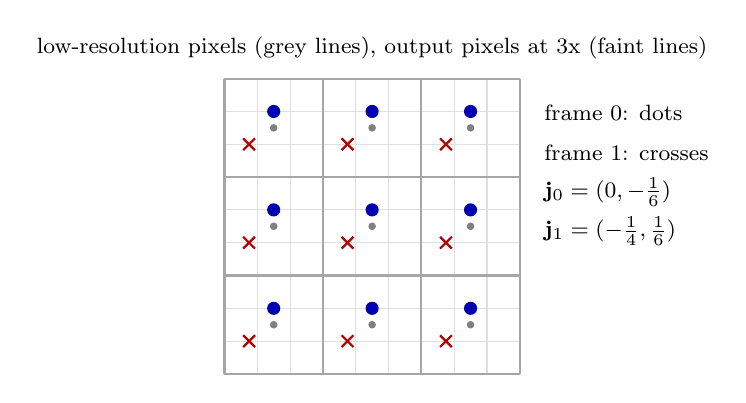
\begin{tikzpicture}[scale=1.25]
  \foreach \k in {0,...,9}{
    \draw[gray!25] (\k/3,-3) -- (\k/3,0);
    \draw[gray!25] (0,-\k/3) -- (3,-\k/3);
  }
  \draw[gray!70, thick] (0,-3) grid (3,0);
  \foreach \i in {0,1,2}{
    \foreach \j in {0,1,2}{
      \fill[gray] (\i+0.5,-\j-0.5) circle (1.1pt);
      \fill[blue!70!black] (\i+0.5,-\j-0.5+0.1667) circle (1.9pt);
      \draw[red!70!black, thick] (\i+0.25-0.06,-\j-0.6667-0.06) -- (\i+0.25+0.06,-\j-0.6667+0.06);
      \draw[red!70!black, thick] (\i+0.25-0.06,-\j-0.6667+0.06) -- (\i+0.25+0.06,-\j-0.6667-0.06);
    }
  }
  \node[anchor=south, font=\footnotesize] at (1.5,0.1) {low-resolution pixels (grey lines), output pixels at 3x (faint lines)};
  \node[anchor=west, font=\footnotesize] at (3.15,-0.35) {frame $0$: dots};
  \node[anchor=west, font=\footnotesize] at (3.15,-0.75) {frame $1$: crosses};
  \node[anchor=west, font=\footnotesize] at (3.15,-1.15) {$\mathbf j_0=(0,-\tfrac16)$};
  \node[anchor=west, font=\footnotesize] at (3.15,-1.55) {$\mathbf j_1=(-\tfrac14,\tfrac16)$};
\end{tikzpicture}
\caption{Sample positions of two consecutive frames inside a $3\times3$ patch of low-resolution pixels, with rows increasing downwards as in the code. Grey dots mark the pixel centres. Blue dots are the samples of frame $0$ and red crosses those of frame $1$, shifted by the first two Halton offsets of \cref{tab:bg-halton}. Faint lines mark the output pixels at 3x, which at this scale subdivide each low-resolution pixel into nine cells.}\label{fig:bg-jitter}
\end{figure}

\paragraph{Halton sequence.} The offsets come from the Halton $(2,3)$ sequence, a low-discrepancy sequence whose points spread evenly over the unit square with fewer large gaps than random points.\cite{halton1960efficiency} For an integer $n\ge1$ with base-$b$ digits $n=\sum_k d_k(n)\,b^k$, the radical inverse is
\begin{equation}
\varphi_b(n)=\sum_{k\ge0}d_k(n)\,b^{-(k+1)}.\label{eq:bg-halton}
\end{equation}
For example, $3=11_2$ gives $\varphi_2(3)=\tfrac12+\tfrac14=\tfrac34$, and $3=10_3$ gives $\varphi_3(3)=\tfrac19$. The function \texttt{halton} computes this by repeated division by the base. Frame $t$ uses the index $n_t=(t\bmod16)+1$ and the offset
\begin{equation}
\mathbf j_t=\big(\varphi_2(n_t)-\tfrac12,\ \varphi_3(n_t)-\tfrac12\big),\label{eq:bg-jitter}
\end{equation}
so the sequence repeats every 16 frames. The index starts at 1 because index 0 would give the corner $(-0.5,-0.5)$. Training gives each sample a random starting point in the cycle. \Cref{tab:bg-halton} lists the first four offsets, which \texttt{jitter\_sequence} produces.

\begin{table}[!htbp]
\caption{First four Halton jitter offsets. Frame $t$ uses index $n=(t\bmod16)+1$, and the offset $\mathbf j_t$ of Eq.~(\ref{eq:bg-jitter}) is in low-resolution pixels. The values were printed by \texttt{jitter\_sequence} and are rounded to three decimals}\label{tab:bg-halton}
\begin{tabular*}{\columnwidth}{@{\extracolsep\fill}rrrrrr}
\toprule
Frame $t$ & $n$ & $\varphi_2(n)$ & $\varphi_3(n)$ & $j_x$ & $j_y$ \\
\midrule
0 & 1 & $0.500$ & $0.333$ & $0.000$ & $-0.167$ \\
1 & 2 & $0.250$ & $0.667$ & $-0.250$ & $0.167$ \\
2 & 3 & $0.750$ & $0.111$ & $0.250$ & $-0.389$ \\
3 & 4 & $0.125$ & $0.444$ & $-0.375$ & $-0.056$ \\
\botrule
\end{tabular*}
\end{table}

\paragraph{Why jitter and accumulation recover resolution.} Take a static scene and one jittered sample per low-resolution pixel per frame. If the samples of earlier frames are placed at their true positions, using each frame's known offset, then after $N$ frames each low-resolution pixel holds $N$ samples at $N$ different positions. The output needs $s^2$ pixels per low-resolution pixel, so the samples must cover the $s^2$ sub-cells, and the Halton positions do this within a few frames. Jitter-aware upsampling does the placement: it samples the low-resolution frame at the output pixel centre minus the jitter (\texttt{jitter\_upsample}), so each sample lands at its true position.

Accumulation is a weighted average. Consider an exponential average $\hat y=\sum_{k\ge0}w_kx_{t-k}$ with weights $w_k=\alpha(1-\alpha)^k$, $0<\alpha\le1$, which sum to one. For samples $x_{t-k}$ with independent noise of variance $\sigma^2$,
\begin{equation}
\operatorname{Var}\hat y=\sum_{k\ge0}w_k^2\sigma^2=\frac{\alpha^2\sigma^2}{1-(1-\alpha)^2}=\frac{\alpha}{2-\alpha}\,\sigma^2,
\end{equation}
so the average behaves like a mean of $N_{\text{eff}}=(2-\alpha)/\alpha$ independent samples. For $\alpha=0.1$, the blend used by the analytic baseline of \cref{sec:bg-taa}, $N_{\text{eff}}=19$. This holds only when the history is aligned, so that a sample from an earlier frame belongs to the same surface point, and when the content is static. Motion and disocclusion break both conditions, which is why the next subsections need reprojection and rejection.

\subsection{Motion vectors and optical flow}\label{sec:bg-motion}

\paragraph{Flow.} For frames $t$ and $s$, the flow $F_{t\to s}$ is a field of displacements in pixels. For a pixel $\mathbf p$ of frame $t$, the point $\mathbf p+F_{t\to s}(\mathbf p)$ is the position in frame $s$ of the surface point that $\mathbf p$ shows in frame $t$. The code uses the backward convention for warping, in which the field is defined on the grid of the frame being produced, $t$, and points into the source frame $s$. Frame $t$ is then predicted from frame $s$ by
\begin{equation}
\hat I_t(\mathbf p)=I_s\big(\mathbf p+F_{t\to s}(\mathbf p)\big),\label{eq:bg-flow}
\end{equation}
which is the backward warp of \cref{sec:bg-warp}. A forward flow $F_{s\to t}$ is defined on the grid of the source frame and points forward. Datasets often store forward flow, and warping with it needs a scatter step that leaves holes and overlaps, so the code converts or reverses the flow instead. The code uses these conventions:
\begin{itemize}
\item Temporal super-resolution: the motion vector of frame $t$ is $m_t=F_{t\to t-1}$, the displacement from the current frame to the previous one, at low-resolution pixels (\texttt{sr\_batch}, \texttt{raft\_mv\_and\_valid}).
\item Frame generation: the engine motion vector of the newest real frame is $M_1=F_{1\to0}$, the displacement from $I_1$ to $I_0$ (\texttt{fg\_batch}).
\item Frame generation: the intermediate flows are $F_{\tau\to0}$ and $F_{\tau\to1}$, the outputs of \texttt{IFNet} (\cref{sec:bg-interp}).
\item Exact sources: the loader plays clips with forward flow backwards (\texttt{load\_clip}). The stored flow from frame $i$ to frame $i+1$ then becomes the displacement from the later frame to the earlier one, which is the convention of $m_t$, without any inversion.
\end{itemize}

\paragraph{Engine vectors and colour flow.} An engine writes a motion vector per pixel from the transforms of the geometry it draws. The vector is exact for opaque surfaces that the engine transforms, and particles and other effects without a transform get none, which is why engines also write a reactive mask. Research systems use such engine buffers, including motion vectors, as network inputs.\cite{xiao2020nsrr} Colour-only flow estimates motion from the images. It works on any video, but it is an estimate that can be wrong at boundaries, and it cannot separate motion from a change of lighting or from an overlay that moves independently. The code uses torchvision's RAFT-Small \cite{teed2020raft} with 12 updates (\texttt{load\_raft}, \texttt{raft\_flow}), as the teacher for motion labels on real video and for tOF. The built-in motion estimator of the temporal super-resolution network is an IFNet \cite{huang2022rife}.

\paragraph{Forward-backward consistency.} For two frames $a$ and $b$ with flows $F_{a\to b}$ and $F_{b\to a}$, a pixel passes the round-trip test when
\begin{equation}
\big\|F_{a\to b}(\mathbf p)+F_{b\to a}\big(\mathbf p+F_{a\to b}(\mathbf p)\big)\big\|<1+0.05\,\big\|F_{a\to b}(\mathbf p)\big\|,\label{eq:bg-fb}
\end{equation}
which says that going to frame $b$ and back returns to the start within one pixel plus 5 percent of the flow. The code's \texttt{raft\_mv\_and\_valid} applies this test with $a$ the current frame and marks the pixels that pass as valid. Pixels that fail lie at occlusions, at disocclusions and where the flow estimate is poor.

\paragraph{Occlusion and disocclusion.} A surface point is disoccluded in frame $t$ when it is visible in $t$ but absent from the previous frame $s$, and it is occluded when it is visible in $s$ but covered in $t$. The warp of Eq.~(\ref{eq:bg-flow}) has no correct source for a disoccluded pixel, so history must not be used there. The code's validity mask $v$ equals 1 where the pixel of frame $t$ is visible in the previous frame, so $1-v$ marks the disoccluded pixels (\texttt{load\_valid}). The temporal super-resolution network also uses a depth cue, $|d_t-\mathcal W(d_{t-1})|/(|d_t|+10^{-3})$, clipped to $[0,1]$, as an input feature (\texttt{TSRNet.forward}).

\paragraph{Scene cuts.} A cut is a change of content between consecutive frames. No point corresponds across it, so any flow is meaningless, and no frame can be predicted from the one before. The code detects cuts with the distance between normalised 32-bin histograms of the luma (\texttt{cut\_score}),
\begin{equation}
d_{\text{hist}}(I_0,I_1)=\tfrac12\sum_{b=1}^{32}\big|h_0(b)-h_1(b)\big|,\label{eq:bg-cut}
\end{equation}
where $h_0$ and $h_1$ are the normalised histograms of the two frames. This distance lies in $[0,1]$ and is the total-variation distance between the two histograms. When the motion vector $M_1$ is available, the score adds $2\,\overline{|I_1-\mathcal W(I_0,M_1)|}$, twice the mean motion-compensated difference. A score above a threshold is a cut.

\subsection{Warping, reprojection and history accumulation}\label{sec:bg-warp}

\paragraph{Backward warping.} Given a frame $I$ and a flow $F$, the warp $\mathcal W(I,F)(\mathbf p)=I(\mathbf p+F(\mathbf p))$ must be evaluated at non-integer positions. The code uses bilinear interpolation. For $\mathbf q=\mathbf p+F(\mathbf p)$ with integer part $(x_0,y_0)$ and fractional parts $a=q_x-x_0$ and $b=q_y-y_0$,
\begin{equation}\begin{split}
I(\mathbf q)&=(1-a)(1-b)\,I(x_0,y_0)+a(1-b)\,I(x_0+1,y_0)\\
&\quad+(1-a)b\,I(x_0,y_0+1)+ab\,I(x_0+1,y_0+1).
\end{split}\label{eq:bg-warp}\end{equation}
The four weights are non-negative and sum to one. Positions outside the frame are clamped to the border. Backward warping gathers each output pixel from one source location, so the output has no holes or overlaps, which forward splatting cannot guarantee. \texttt{backward\_warp} implements Eq.~(\ref{eq:bg-warp}) with \texttt{grid\_sample}, using the coordinate mapping of RIFE, in which pixel index $i$ corresponds to the normalised coordinate $-1+2i/(W-1)$. \Cref{fig:bg-warp} shows one pixel.

\begin{figure}[!htbp]
\centering
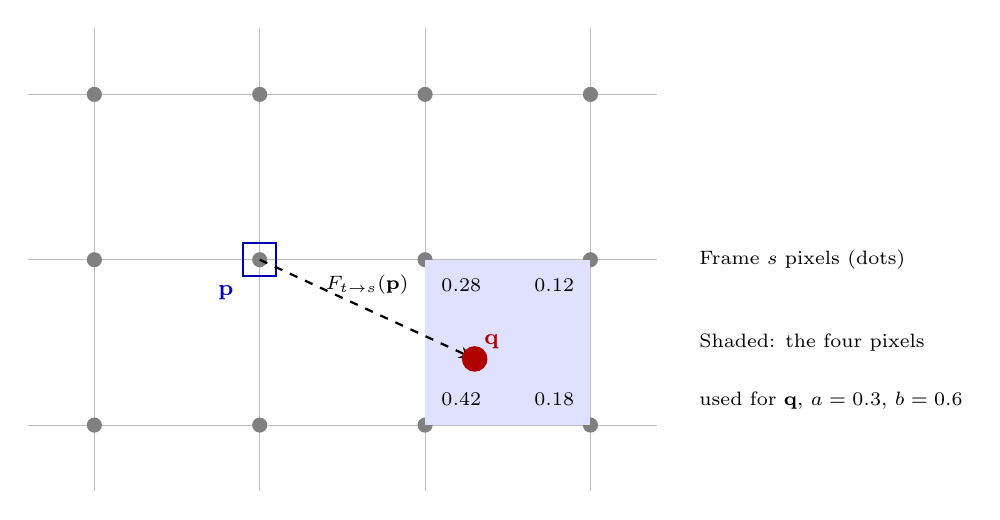
\begin{tikzpicture}[scale=2.1, font=\footnotesize]
  \draw[gray!50] (-0.4,-2.4) grid (3.4,0.4);
  \foreach \i in {0,...,3}{\foreach \j in {0,...,2}{\fill[gray] (\i,-\j) circle (1.3pt);}}
  \fill[blue!12] (2,-2) rectangle (3,-1);
  \draw[blue!70!black, thick] (0.9,-0.9) rectangle (1.1,-1.1);
  \node[anchor=north east, text=blue!70!black] at (0.9,-1.1) {$\mathbf p$};
  \draw[-{Stealth[length=2mm]}, thick, dashed] (1,-1) -- (2.3,-1.6);
  \node[anchor=south, font=\scriptsize] at (1.65,-1.27) {$F_{t\to s}(\mathbf p)$};
  \fill[red!70!black] (2.3,-1.6) circle (2.2pt);
  \node[anchor=south west, text=red!70!black] at (2.3,-1.6) {$\mathbf q$};
  \node[anchor=north west] at (2.04,-1.06) {\scriptsize $0.28$};
  \node[anchor=north east] at (2.96,-1.06) {\scriptsize $0.12$};
  \node[anchor=south west] at (2.04,-1.94) {\scriptsize $0.42$};
  \node[anchor=south east] at (2.96,-1.94) {\scriptsize $0.18$};
  \node[anchor=west] at (3.6,-1.0) {\scriptsize Frame $s$ pixels (dots)};
  \node[anchor=west] at (3.6,-1.5) {\scriptsize Shaded: the four pixels};
  \node[anchor=west] at (3.6,-1.85) {\scriptsize used for $\mathbf q$, $a=0.3$, $b=0.6$};
\end{tikzpicture}
\caption{Backward warp of one pixel. Pixel $\mathbf p=(1,1)$ of frame $t$ takes the value at $\mathbf q=\mathbf p+F_{t\to s}(\mathbf p)=(2.3,1.6)$ in frame $s$. That value is the bilinear mixture of the four surrounding pixels of frame $s$, with the weights shown from Eq.~(\ref{eq:bg-warp}). The flow is illustrative.}\label{fig:bg-warp}
\end{figure}

\paragraph{Half-pixel attenuation.} Bilinear interpolation is a low-pass filter. For a shift of half a pixel the weights are $(\tfrac12,\tfrac12)$, and the frequency response at angular frequency $\omega$ radians per pixel is $\tfrac12(1+e^{-i\omega})$, whose magnitude is $|\cos(\omega/2)|$. At $\omega=\pi/2$ this is $\cos(\pi/4)\approx0.71$, and at the Nyquist frequency $\omega=\pi$ it is zero. Each warp at a fractional offset removes part of the high-frequency content. A recurrent network that warps its output every frame loses high frequencies at every step unless its residual path adds them back.

\paragraph{Reprojection and accumulation.} Reprojection moves a stored result to the current frame. A history image $H$ from frame $t-1$ becomes $H_t(\mathbf p)=\mathcal W(H,m_t)(\mathbf p)$ with $m_t=F_{t\to t-1}$, and accumulation then combines $H_t$ with the new samples. The recurrent state of the temporal super-resolution network, its output and its hidden feature map, is reprojected in the same way with the low-resolution vectors. A pixel whose motion is wrong, or which is disoccluded, takes its history from the wrong surface, and that is the source of the ghosting described in \cref{sec:bg-taa}.

\subsection{Temporal anti-aliasing and temporal upscaling}\label{sec:bg-taa}

Temporal anti-aliasing (TAA) \cite{yang2020taasurvey} combines jittered samples over time with a history buffer. For each frame it renders with a jittered sample grid, reprojects the history with motion vectors, clamps the reprojected history to the range of the current samples in a small neighbourhood, and blends the clamped history with the current samples. Temporal upscaling runs the same loop at a lower render resolution, with the accumulation buffer at output resolution.

\paragraph{Exponential blending.} Without reprojection and clamping, accumulation is $\hat y_t=\alpha x_t+(1-\alpha)\hat y_{t-1}$, where $x_t$ is the current sample value and $0<\alpha\le1$. Unrolling gives
\begin{equation}
\hat y_t=\sum_{k=0}^{t-1}\alpha(1-\alpha)^k\,x_{t-k}+(1-\alpha)^t\,\hat y_0,\label{eq:bg-ema-unroll}
\end{equation}
so the sample $k$ frames old has weight $\alpha(1-\alpha)^k$, and the initial value keeps the weight $(1-\alpha)^t$. \Cref{fig:bg-ema} shows these weights for $\alpha=0.1$. A sample 10 frames old has weight $0.035$, and the initial value still has weight $0.12$ after 20 frames.

\begin{figure}[!htbp]
\centering
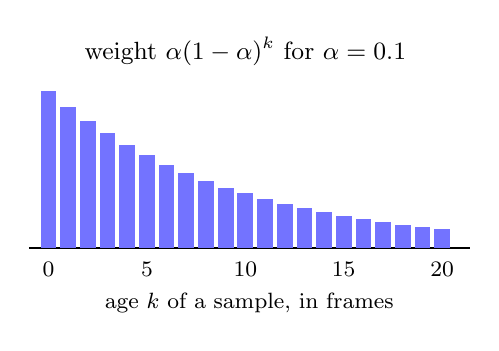
\begin{tikzpicture}[x=0.5cm, font=\footnotesize]
  \draw[thick] (-0.3,0) -- (10.9,0);
  \foreach \k/\h in {0/2.00,1/1.80,2/1.62,3/1.46,4/1.31,5/1.18,6/1.06,7/0.96,8/0.86,9/0.77,10/0.70,11/0.63,12/0.56,13/0.51,14/0.46,15/0.41,16/0.37,17/0.33,18/0.30,19/0.27,20/0.24}{
    \fill[blue!55] (\k*0.5,0) rectangle (\k*0.5+0.4,\h);
  }
  \foreach \k in {0,5,10,15,20}{
    \node[below] at (\k*0.5+0.2,-0.05) {\k};
  }
  \node[below] at (5.3,-0.45) {age $k$ of a sample, in frames};
  \node[above] at (5.2,2.2) {\small weight $\alpha(1-\alpha)^k$ for $\alpha=0.1$};
\end{tikzpicture}
\caption{Weight of a sample $k$ frames old in the exponential average of \cref{eq:bg-ema-unroll} with $\alpha=0.1$. The bar height is the weight times 20, in centimetres of the drawing. The weights fall geometrically, so an old surface that stays in the history fades slowly, which is the ghosting trail that clamping limits.}\label{fig:bg-ema}
\end{figure}

\paragraph{Ghosting.} When a surface changes, because it is disoccluded, because its motion vector is wrong or because an object leaves a region, the history still holds the old surface. That surface keeps the weight $(1-\alpha)^k$ for $k$ frames and appears as a trail behind moving objects. Clamping limits the trail. The reprojected value is confined to the range of the current neighbourhood, so an old colour far from the new samples is pulled back to the range boundary. Ghosting remains when the old colour lies inside that range, which happens when a surface and its background have similar colours. A larger $\alpha$ reduces ghosting but also reduces the averaging that removes aliasing, and that trade-off is the central design choice of TAA.

\paragraph{Analytic baseline.} The analytic upscaler of the evaluation (\texttt{AnalyticTAAU} in \texttt{nss\_metrics.py}, run by \texttt{run\_taau} in \texttt{nss\_eval.py}) implements the loop with fixed rules and stands in for analytic TAA upscalers without their proprietary heuristics. For frame $t$, with low-resolution colour $x_t$, jitter $\mathbf j_t$ and low-resolution motion vector $m_t$, it performs the following steps.
\begin{enumerate}
\item Base image: $B_t(\mathbf p)$ is the bilinear interpolation of $x_t$ at the low-resolution position of the output pixel centre $\mathbf p$ minus $\mathbf j_t$, so each sample is placed at its true position.
\item If there is no history, the output is $B_t$.
\item History: $H_t=\mathcal W\big(\hat y_{t-1},\,s\,U(m_t)\big)$, where $U$ is bilinear upsampling by $s$ and the factor $s$ converts low-resolution displacements into output pixels.
\item Clamp: with $lo$ and $hi$ the channel-wise minimum and maximum of YCoCg$(B_t)$ over the $3\times3$ output neighbourhood of each pixel, the history is clamped in YCoCg to the box between $lo$ and $hi$, and $H'_t$ is the RGB value of the clamped history.
\item Blend: $\hat y_t=H'_t+0.1\,(B_t-H'_t)$, which is 90 percent history and 10 percent current base image.
\end{enumerate}
The displayed output is clamped to $[0,1]$, but the unclamped value becomes the next history. Step 5 gives
\begin{equation}
\hat y_t=0.9\,H'_t+0.1\,B_t.\label{eq:bg-taa}
\end{equation}

Two properties of this baseline matter for the comparison. First, its docstring says that it resets on invalid history, but the code has no validity test, so every frame reprojects and clamps the history and no disocclusion rejection takes place. Second, the motion vectors are sampled at the jittered sample positions (\texttt{\_sr\_inputs}), while the baseline interprets low-resolution vectors as if they were at the pixel centres. The resulting error is the jitter times the local gradient of the motion field, which vanishes for uniform motion and is largest at motion boundaries. The temporal super-resolution network receives the same low-resolution vectors and interprets them in the same way. The supplement describes these properties as they are in the code.

\subsection{Neural building blocks}\label{sec:bg-cnn}

The networks use a small set of operators. Each is defined here with the code's convention and with the reason for its use.

\paragraph{Convolution and multiply-accumulates.} A convolutional layer with $C_{\text{in}}$ input channels, $C_{\text{out}}$ output channels and a $k\times k$ kernel $K$ computes, with stride 1 and padding $(k-1)/2$,
\begin{equation}
Y[o,i,j]=b_o+\sum_{c=1}^{C_{\text{in}}}\sum_{u=0}^{k-1}\sum_{v=0}^{k-1}K[o,c,u,v]\;X\!\Big[c,\;i+u-\tfrac{k-1}{2},\;j+v-\tfrac{k-1}{2}\Big],\label{eq:bg-conv}
\end{equation}
where $X$ is the input, $Y$ the output and $b_o$ the bias of output channel $o$. The sum is a cross-correlation, which is PyTorch's convention. One multiply-accumulate (MAC) is one multiplication followed by one addition. Each output element of Eq.~(\ref{eq:bg-conv}) costs $C_{\text{in}}k^2$ MACs, so a layer with an $H\times W$ output costs
\begin{equation}
M=H\,W\,C_{\text{out}}\,C_{\text{in}}\,k^2\qquad\text{MACs},\label{eq:bg-macs}
\end{equation}
and grouped convolutions divide this by the number of groups. A transposed convolution from an $H_{\text{in}}\times W_{\text{in}}$ input costs $H_{\text{in}}W_{\text{in}}C_{\text{in}}C_{\text{out}}k^2$, because each input pixel scatters a $k\times k$ kernel into every output channel. Pixel shuffles, bilinear resizing and grid sampling perform no such multiply-accumulates in the count, so the warps are excluded from the cost figures, as in \cref{M-tab:tiers}. For example, a $3\times3$ convolution with 24 input and 24 output channels costs $24\cdot24\cdot9=5{,}184$ MACs per output pixel.

\paragraph{Cost per 1080p frame.} The code counts MACs with forward hooks (\texttt{count\_macs}) on the fused network, which is the deployed form in which every block is a plain convolution. For temporal super-resolution it runs one step with a history state on a $64\times64$ low-resolution input, including the built-in motion estimator, and divides the count by $64^2$ to obtain MACs per low-resolution pixel (\texttt{tsr\_macs\_per\_lr\_pixel}). Each layer's cost is proportional to its pixel count, so the cost of one output frame is that per-pixel count times the number of low-resolution pixels of the 1080p output,
\begin{equation}
G_{1080p}=\frac{M_{\text{pix}}\,(1920/s)(1080/s)}{10^{9}}\quad\text{GMAC}.\label{eq:bg-gmac}
\end{equation}
For frame generation the fused network runs on a $272\times480$ frame. The flow-resolution limit is scaled by $272/1080$ so that the flow runs at the scale that a 1080p frame would use, the MACs are counted, and the count is multiplied by $(1920\cdot1080)/(272\cdot480)$. This assumes that the cost is linear in the pixel count, which holds for convolutions and is approximate for the remaining operators. A MAC count is a cost measure and not a time, and the latency measurements are reported separately.

\paragraph{Pixel shuffle.} Pixel shuffle \cite{shi2016espcn} rearranges a tensor with $C r^2$ channels at $H\times W$ into $C$ channels at $rH\times rW$,
\begin{equation}
Z[c,\;rh+a,\;rw+b]=X[c\,r^2+a\,r+b,\;h,\;w],\qquad 0\le a,b<r,\label{eq:bg-shuffle}
\end{equation}
without any multiplication. Its inverse, pixel unshuffle or space-to-depth, folds a tensor at $rH\times rW$ into $r^2$ times as many channels at $H\times W$. A convolution can therefore run at low resolution, where it is cheap, and the shuffle restores the output size. The temporal super-resolution network uses both directions. Its output convolution produces $4s^2$ channels at low resolution, which the shuffle turns into a residual and a history weight at output resolution, and it folds the reprojected output into $3s^2$ low-resolution channels before the trunk reads it.

\paragraph{Structural re-parameterisation.} A block can be trained as several parallel linear branches and deployed as one convolution. This works when the branches share their input and their spatial support, because convolution is linear in its kernel. The RepConv block of \texttt{nss\_models.py} has four branches on the same input $x$, with $C_{\text{in}}$ input and $C_{\text{out}}$ output channels:
\begin{enumerate}
\item a $3\times3$ convolution with kernel $W_3$ and bias $b_3$.
\item a $1\times1$ convolution with kernel $W_1$ and bias $b_1$.
\item the identity, present when $C_{\text{in}}=C_{\text{out}}$.
\item fixed edge filters $E_1$ (Sobel $x$), $E_2$ (Sobel $y$) and $E_3$ (Laplacian), applied to every input channel, whose $3C_{\text{in}}$ responses are combined by a learned $1\times1$ projection $P\in\mathbb R^{C_{\text{out}}\times3C_{\text{in}}}$ with bias $b_e$.
\end{enumerate}
The block output is $\phi(Y)$, where $\phi$ is a PReLU activation and $Y$ is the sum of the four branch outputs.

The four branches fold into one $3\times3$ convolution, exactly:
\begin{equation}\begin{split}
Y&=\sum_{c}K[\cdot,c]\ast x_c+b,\\
K[o,c]&=W_3[o,c]+\operatorname{pad}\big(W_1[o,c]\big)\\
&\quad+\sum_{k=1}^{3}\tilde P[o,c,k]\,E_k+\delta_{oc}\,\Delta,\\
b&=b_3+b_1+b_e,
\end{split}\label{eq:bg-fold}\end{equation}
where $\ast$ is convolution with stride 1 and padding 1, $\operatorname{pad}$ places a scalar at the centre tap of an otherwise zero $3\times3$ kernel, $\tilde P[o,c,k]=P[o,\,3c+k]$ reorders the projection by input channel, $\delta_{oc}$ is the Kronecker delta and $\Delta$ is the $3\times3$ kernel with 1 at its centre and 0 elsewhere.

\emph{Proof.} Each branch is linear in $x$ and is a convolution with stride 1 and padding 1, so each can be written as a $3\times3$ convolution. (1) The $1\times1$ branch outputs $W_1[o,c]\,x_c(\mathbf p)$. With padding 1, a $3\times3$ kernel whose only nonzero tap is the centre, with value $W_1[o,c]$, produces the same output, and that kernel is $\operatorname{pad}(W_1[o,c])$. (2) The identity outputs $x_o(\mathbf p)$, which is the kernel $\Delta$ on the diagonal $c=o$. (3) The edge branch outputs $\sum_c\sum_k P[o,3c+k]\,(E_k\ast x_c)(\mathbf p)+b_e[o]$. Convolution is linear in its kernel, so $\sum_k\tilde P[o,c,k]\,(E_k\ast x_c)=\big(\sum_k\tilde P[o,c,k]E_k\big)\ast x_c$, and the branch is a $3\times3$ convolution with kernel $\sum_k\tilde P[o,c,k]E_k$ and bias $b_e[o]$. (4) For a common stride and padding, $(A\ast x)+(B\ast x)=(A+B)\ast x$, so the four branch sums combine into Eq.~(\ref{eq:bg-fold}). The activation is applied after the sum, so it is not folded, and the fold is exact. Up to floating-point rounding, the fused and unfused outputs are identical, and the code's fusion-parity test checks this numerically. $\square$

Training uses the folded kernel directly. The code recomputes $K$ from the branch parameters on every forward pass (online re-parameterisation), so a block costs one $3\times3$ convolution during training as well as in deployment. The function class is unchanged, because $W_3$ alone can represent any kernel that the block can reach. The extra branches only change which kernels gradient descent reaches. The $1\times1$ and edge-projection weights start at zero, so the block starts as a $3\times3$ convolution plus the identity. Only the weights are zeroed, so the small biases $b_1$ and $b_e$ remain at their random initial values. \Cref{fig:bg-fold} summarises the fold.

\begin{figure}[!htbp]
\centering
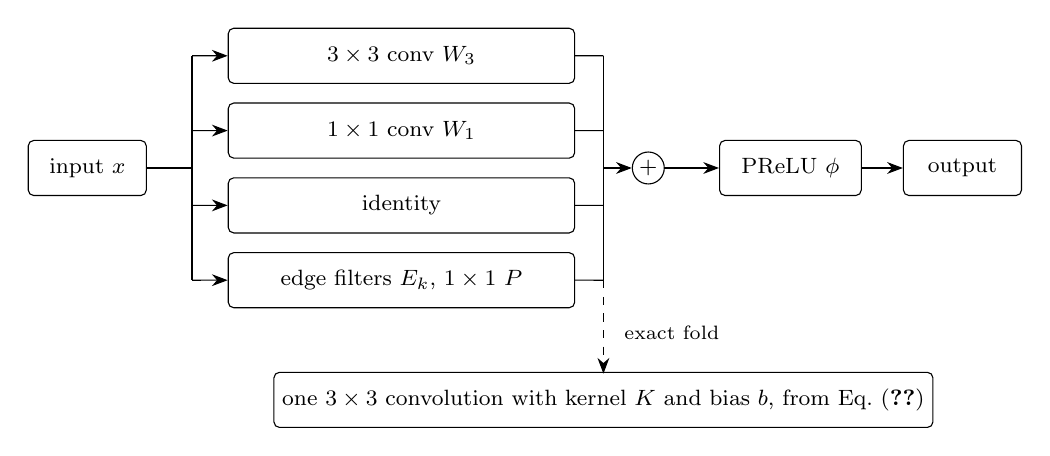
\begin{tikzpicture}[scale=0.95, font=\footnotesize, node distance=3mm,
  box/.style={draw, rounded corners=2pt, align=center, minimum height=7mm, minimum width=4.4cm, inner sep=3pt},
  arr/.style={-{Stealth[length=2mm]}}]
\node[box, minimum width=1.5cm] (x) at (0,0) {input $x$};
\node[box] (w3) at (4.2,1.5) {$3\times3$ conv $W_3$};
\node[box] (w1) at (4.2,0.5) {$1\times1$ conv $W_1$};
\node[box] (id) at (4.2,-0.5) {identity};
\node[box] (ed) at (4.2,-1.5) {edge filters $E_k$, $1\times1$ $P$};
\node[draw, circle, inner sep=1pt] (sum) at (7.5,0) {$+$};
\node[box, minimum width=1.8cm] (act) at (9.4,0) {PReLU $\phi$};
\node[box, minimum width=1.5cm] (out) at (11.7,0) {output};
\draw (x.east) -- (1.4,0);
\draw (1.4,1.5) -- (1.4,-1.5);
\draw[arr] (1.4,1.5) -- (w3.west);
\draw[arr] (1.4,0.5) -- (w1.west);
\draw[arr] (1.4,-0.5) -- (id.west);
\draw[arr] (1.4,-1.5) -- (ed.west);
\draw (w3.east) -- (6.9,1.5);
\draw (w1.east) -- (6.9,0.5);
\draw (id.east) -- (6.9,-0.5);
\draw (ed.east) -- (6.9,-1.5);
\draw (6.9,1.5) -- (6.9,-1.5);
\draw[arr] (6.9,0) -- (sum.west);
\draw[arr] (sum.east) -- (act.west);
\draw[arr] (act.east) -- (out.west);
\node[box, minimum width=7.0cm] (k) at (6.9,-3.1) {one $3\times3$ convolution with kernel $K$ and bias $b$, from Eq.~(\ref{eq:bg-fold})};
\draw[arr, dashed] (6.9,-1.5) -- (6.9,-2.75);
\node[anchor=west, font=\scriptsize] at (7.05,-2.2) {exact fold};
\end{tikzpicture}
\caption{Re-parameterisation of one RepConv block. The four linear branches share the input and sum before the activation, giving one kernel $K$ and bias $b$ of size $3\times3$.}\label{fig:bg-fold}
\end{figure}

\paragraph{U-Net levels.} The trunk of the temporal super-resolution network has an optional half-resolution level. It differs from the classic U-Net,\cite{ronneberger2015unet} so it is described precisely here. A strided $3\times3$ convolution halves the resolution and doubles the channels. Residual blocks run at half resolution, a $1\times1$ convolution doubles the channels to $4w$, and a pixel shuffle returns to full resolution with $w$ channels. The result is added to the features that entered the level, which is an additive skip, where the classic U-Net concatenates. A convolution with $2w$ channels at half resolution costs the same as one with $w$ channels at full resolution, because $(2w)^2\cdot\tfrac14=w^2$, but each of its taps covers twice the distance in the original image.

\paragraph{Recurrent networks and hidden-state warping.} A recurrent network carries a state from frame to frame. The state of the temporal super-resolution network holds the previous output $\hat y_{t-1}$, a hidden feature map $h_{t-1}$, and the previous depth, colour and jitter. At each frame the network reads the current inputs together with the reprojected output and hidden state, and writes the new output and a new hidden state $h_t=\tanh(\cdot)$ of a convolution. The hidden state is reprojected with the same motion as the output, $\mathcal W(h_{t-1},m_t)$, because its channels describe the content at each pixel, and a feature warped with the wrong motion describes a different surface. Training unrolls the network over several frames, with a 16-frame unroll every fourth step, and backpropagates through the whole unroll, which is backpropagation through time. During the first quarter of training (\texttt{mv\_warmup\_frac} $=0.25$), samples without motion vectors warp the history with the label motion instead of the estimated motion. The probability of doing so falls linearly from one to zero over that quarter. Feeding the label in place of the model's own estimate is teacher forcing, which this code applies as a schedule, and the schedule stops the history path from learning to ignore history while the estimator is still poor.

\paragraph{Zero initialisation.} A branch whose output layer has zero weights and a zero bias contributes exactly zero at initialisation, so the network starts as the network without that branch. Two consequences follow. The output layer receives a nonzero gradient, because its input features are nonzero, so it learns from the first step. The layers upstream of it receive a zero gradient at the first step, because they reach the loss only through the zero weights, and they start to learn once the output layer is nonzero. The bias must also be zero, because a nonzero bias gives a constant contribution at initialisation. The code uses three instances.
\begin{itemize}
\item The engine-hint input channels of the first convolution in each IFNet block have zero weights, so the hints do not change that layer's output at initialisation. This is exact.
\item The frame generator's residual head has zero weights and a zero bias, so its colour residual $r$ is zero at initialisation. Its UI logit has a bias of $-4$, so the UI weight is $u=\sigma(-4)\approx0.018$ at initialisation. The output is therefore $u\,I_1+(1-u)$ times the RIFE blend $m\mathcal W(I_0,F_{\tau\to0})+(1-m)\mathcal W(I_1,F_{\tau\to1})$, and differs from that blend by $u\,(I_1-\text{blend})$. The code's parity test compares the blend, not the final output, so a fresh model reproduces the blend of RIFE exactly and not its final output.
\item The temporal super-resolution output layer has zero weights and a zero bias, so the residual is zero and the history weight is $\sigma(0+2)\approx0.88$, since the code adds 2 to the logit before the sigmoid. At initialisation the output is therefore $0.88$ of the history and $0.12$ of the jitter-aware upsampling, an exponential blend of the kind described in \cref{sec:bg-taa}.
\end{itemize}

\paragraph{Mixed precision and loss scaling.} In IEEE half precision (FP16) a value has one sign bit, five exponent bits and ten fraction bits. Its largest finite value is $(2-2^{-10})\,2^{15}=65{,}504$, its smallest positive normal value is $2^{-14}\approx6.1\cdot10^{-5}$, and its smallest positive subnormal value is $2^{-24}\approx6.0\cdot10^{-8}$. Two failures follow. Activations above 65{,}504 become infinite, and gradients much smaller than $6\cdot10^{-8}$ round to zero. Mixed precision \cite{micikevicius2018mixed} runs the forward and backward passes in FP16 and keeps FP32 copies of the weights. Loss scaling multiplies the loss by a scale $S$ before the backward pass, so that small gradients stay representable, and divides the gradients by $S$ before the optimiser step. Dynamic loss scaling lowers $S$ when a step produces non-finite gradients and raises it again after a run of finite steps. The code uses PyTorch's \texttt{GradScaler} with autocast. It scales the loss, unscales the gradients, clips their norm to 1.0 (\texttt{grad\_clip}) and then steps the optimiser. A run stops when the loss stays non-finite for 200 steps by default.

\paragraph{Exponential moving average.} The optimiser updates the weights $w_k$, and the code also keeps the average
\begin{equation}
\bar w_k=d_k\,\bar w_{k-1}+(1-d_k)\,w_k,\qquad d_k=\min\!\Big(0.999,\ \frac{1+k}{10+k}\Big),\label{eq:bg-ema}
\end{equation}
which is used for validation and checkpoints, while the raw weights produce the gradients. The warm-up in $d_k$ means that the decay reaches 0.999 only after about 9{,}000 steps, so early in training the average follows the weights closely. At a decay of 0.999 the average has a memory of about $1/(1-0.999)=1{,}000$ steps.

\paragraph{AdamW.} AdamW \cite{loshchilov2019adamw} keeps running averages of the gradient and of its square, $m_k=\beta_1 m_{k-1}+(1-\beta_1)g_k$ and $v_k=\beta_2 v_{k-1}+(1-\beta_2)g_k^2$, corrects their start-up bias and applies
\begin{equation}
\theta_k=\theta_{k-1}-\eta\Big(\frac{\hat m_k}{\sqrt{\hat v_k}+\epsilon}+\lambda\,\theta_{k-1}\Big),\qquad \hat m_k=\frac{m_k}{1-\beta_1^k},\quad \hat v_k=\frac{v_k}{1-\beta_2^k},\label{eq:bg-adamw}
\end{equation}
where $g_k$ is the gradient, $\eta$ the learning rate and $\lambda$ the weight decay. The decay term $\lambda\theta$ acts on the weights directly and is not added to the gradient, which is the difference from Adam with an L2 penalty. The code uses $(\beta_1,\beta_2)=(0.9,0.99)$, PyTorch's default $\epsilon=10^{-8}$ and $\lambda=10^{-4}$.

\paragraph{Learning-rate schedule.} The schedule is driven by wall-clock time rather than by the step count. With progress $p\in[0,1]$, the elapsed fraction of the run's time budget, a warm-up fraction $w=0.03$, a peak rate $\eta_0$ and a floor $\eta_{\min}=10^{-6}$,
\begin{equation}
\eta(p)=\begin{cases}\eta_0\,\max(p/w,\,0.01), & p<w,\\[2pt] \eta_{\min}+\tfrac12(\eta_0-\eta_{\min})\big(1+\cos\pi\tau\big), & \tau=\dfrac{p-w}{1-w}\ge0,\end{cases}\label{eq:bg-cosine}
\end{equation}
which is \texttt{lr\_at}. The learning rate follows a single cosine decay without restarts, the decay used within each cycle of SGDR \cite{loshchilov2017sgdr}. The peak rates are $2\cdot10^{-3}$ for the temporal super-resolution student, $10^{-3}$ for its teacher, $4\cdot10^{-4}$ for the frame-generation students and $10^{-4}$ for the frame-generation tier fine-tuned from RIFE 4.26. Because the schedule follows wall-clock time, a slower GPU performs fewer updates in the same budget.

\paragraph{Charbonnier loss.} The Charbonnier penalty \cite{charbonnier1997deterministic} is a smooth edge-preserving potential that approximates the absolute error,
\begin{equation}
\rho_\epsilon(e)=\sqrt{e^2+\epsilon^2},\qquad \epsilon=10^{-3},\label{eq:bg-charb}
\end{equation}
which is differentiable at zero and tends to $|e|$ for large errors. Its gradient $e/\rho_\epsilon(e)$ has magnitude at most one, so large errors do not dominate the gradient as they do under a squared error. The code averages $\rho_\epsilon$ over the elements (\texttt{charbonnier}), with an optional mask that normalises by the number of masked elements.

\subsection{Video frame interpolation and extrapolation}\label{sec:bg-interp}

Given real frames $I_0$ at time 0 and $I_1$ at time 1, interpolation produces $I_\tau$ for $0<\tau<1$. Extrapolation produces $I_\tau$ for $\tau>1$ from frames at or before time 1 only. \Cref{fig:bg-tau} shows the time axis of both modes. Multi-frame generation with a factor $N$ inserts $N-1$ frames between real frames, so 3x generation uses $\tau=\tfrac13$ and $\tau=\tfrac23$. Generation raises the displayed frame rate without rendering the scene again, but it has to wait for the real frame it needs, as \cref{sec:bg-latency} explains.

\begin{figure}[!htbp]
\centering
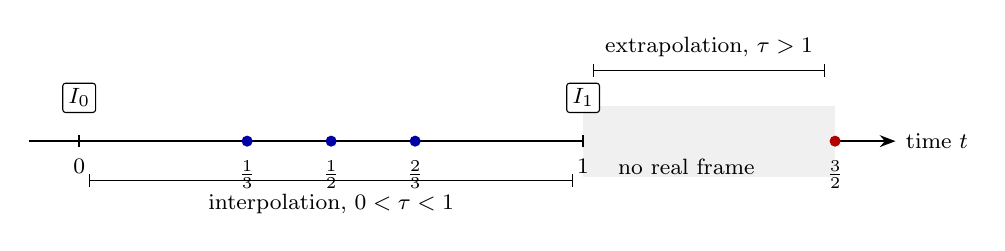
\begin{tikzpicture}[x=6.4cm, font=\footnotesize]
  \draw[thick, -{Stealth[length=2mm]}] (-0.1,0) -- (1.62,0) node[right] {time $t$};
  \fill[gray!12] (1,-0.45) rectangle (1.5,0.45);
  \draw[thick] (0,-0.08) -- (0,0.08);
  \draw[thick] (1,-0.08) -- (1,0.08);
  \node[draw, rounded corners=1pt, fill=white, inner sep=2pt] at (0,0.55) {$I_0$};
  \node[draw, rounded corners=1pt, fill=white, inner sep=2pt] at (1,0.55) {$I_1$};
  \node[below] at (0,-0.1) {$0$};
  \node[below] at (1,-0.1) {$1$};
  \foreach \x/\lab in {0.3333/{$\tfrac13$}, 0.5/{$\tfrac12$}, 0.6667/{$\tfrac23$}}{
    \fill[blue!65!black] (\x,0) circle (2pt);
    \node[below] at (\x,-0.12) {\lab};
  }
  \fill[red!70!black] (1.5,0) circle (2pt);
  \node[below] at (1.5,-0.12) {$\tfrac32$};
  \draw[|-|] (0.02,-0.5) -- (0.98,-0.5);
  \node[below] at (0.5,-0.55) {\footnotesize interpolation, $0<\tau<1$};
  \draw[|-|] (1.02,0.9) -- (1.48,0.9);
  \node[above] at (1.25,0.95) {\footnotesize extrapolation, $\tau>1$};
  \node[anchor=west, font=\footnotesize] at (1.05,-0.32) {no real frame};
\end{tikzpicture}
\caption{Time axis of the two generation modes with real frames $I_0$ and $I_1$. Interpolation (blue) places generated frames between the real frames, at $\tau=\tfrac12$ or at the two positions of 3x generation. Extrapolation (red) places a generated frame after $I_1$ at $\tau=\tfrac32$ using only frames at or before time 1. The shaded interval has no real frame.}\label{fig:bg-tau}
\end{figure}

\paragraph{Intermediate flows.} The generator needs the motion from each real frame to the intermediate time $\tau$, which is $F_{\tau\to0}$ and $F_{\tau\to1}$ as defined in \cref{sec:bg-motion}. Under constant velocity, a surface point moves as $\mathbf p(\tau)=\mathbf p_0+\tau\mathbf v$, where $\mathbf v$ is its displacement from time 0 to time 1, so that $\mathbf p_1=\mathbf p_0+\mathbf v$. Its displacement from $I_1$ to $I_0$ is $M_1=-\mathbf v$, and therefore
\begin{equation}
F_{\tau\to0}=\tau M_1,\qquad F_{\tau\to1}=(\tau-1)M_1,\label{eq:bg-linear}
\end{equation}
which are the linear-motion priors of the frame generator. To see this, note $F_{\tau\to0}=\mathbf p_0-\mathbf p(\tau)=-\tau\mathbf v=\tau M_1$, and $F_{\tau\to1}=\mathbf p_1-\mathbf p(\tau)=(1-\tau)\mathbf v=(\tau-1)M_1$. The code evaluates $M_1$ at the target pixel rather than at the moving point, which is exact when the motion field is locally constant.

\paragraph{Coarse-to-fine estimation.} The intermediate flows come from an IFNet with the design of RIFE 4.26 \cite{huang2022rife}. It is a chain of blocks, each working at a fraction $1/s_k$ of the input resolution, with scales $16,8,4,2,1$ for the five blocks of the full network. Each block predicts a blend logit and an update to the flow at its own resolution. The update is resampled to full resolution and multiplied by $s_k$, because a displacement in pixels scales with resolution, so
\begin{equation}
F^{(k)}=F^{(k-1)}+s_k\,\mathcal U_{s_k}\big(\tilde\Delta^{(k)}\big),\label{eq:bg-c2f}
\end{equation}
where $\tilde\Delta^{(k)}$ is the raw update of block $k$ and $\mathcal U_{s_k}$ is bilinear upsampling by $s_k$. The coarse blocks capture large motion at low cost, and the fine blocks add detail.

\paragraph{Blending.} The two warped frames are combined with a per-pixel blend $m\in[0,1]$, which is the sigmoid of the network's logit,
\begin{equation}
\hat I_\tau=m\odot\mathcal W(I_0,F_{\tau\to0})+(1-m)\odot\mathcal W(I_1,F_{\tau\to1}),\label{eq:bg-blend}
\end{equation}
where $\odot$ is the element-wise product. Where a surface is visible in only one real frame, the correct blend selects that frame, and this is how interpolation handles occlusions.

\paragraph{Resolution rule and cuts.} Flow is costly, so the generator estimates it at a reduced scale for tall frames. The flow scale is the largest $2^{-k}$ with $H\,2^{-k}\le L$, where $L$ is the flow limit of the tier, 576 or 1152 lines. At 1080p this gives 540 lines for $L=576$ and full resolution for $L=1152$. When two real frames come from different scenes, the flows and the blend describe no correspondence, so generation should not run. The code repeats $I_1$ in that case, as \cref{sec:bg-motion} describes. Interpolation also fails where the motion exceeds what the flow search can resolve, at disocclusions where the blend cannot choose, for particles and other motion without correspondence, and on overlays such as text and HUD elements that move differently from the scene.

\subsection{Frame budgets, pacing and latency}\label{sec:bg-latency}

\paragraph{Frame budget.} A display that refreshes $R$ times per second shows a new frame every $1000/R$ milliseconds. That is 16.7 ms at 60 Hz, 33.3 ms at 30 Hz and 8.3 ms at 120 Hz. A renderer that cannot finish a frame within the interval either presents it late or repeats the previous one, so every stage of the frame must fit the budget if the rate is to be sustained. The stages are a CPU update of $c$ ms, a GPU render of $r$ ms, the upscaling of $s$ ms, the frame generation of $g$ ms and the presentation of $p$ ms. In a GPU-bound loop the period is set by the GPU, so the period of a generating loop is $P=\max(c,\,r+s+g)$, the rule that \texttt{simulate\_latency} applies, and the CPU work starts just in time so that no frame waits in a queue.

\paragraph{Three quantities that differ.} Three measures are easily confused.
\begin{itemize}
\item The rendered frame rate is the number of real frames per second that the engine produces, which is $1000/P$ for a loop without generation.
\item The displayed frame rate is the number of frames presented per second, including generated frames. With one generated frame per real frame it is about twice the rendered rate, provided that generation does not lengthen the period, and in a GPU-bound loop it does lengthen it.
\item The input latency is the time from an input sample to the first photons of a frame that reflects it. The frame rate does not determine it.
\end{itemize}

\paragraph{Latency of interpolation and extrapolation.} Interpolation shows a generated frame between $I_{k-1}$ and $I_k$, which needs $I_k$ to exist. The real frame $I_k$ is therefore held until the generated frame has been shown, and it is shown about half a period later, so the input latency of a real frame rises by $g+P/2$. Extrapolation generates from past frames only, so a real frame is presented as soon as it is rendered and its latency does not change. The generated frame follows the real frame, and in the simulator it is presented half a period after it. \Cref{fig:bg-pacing} shows the presentation times that these rules give for one real frame in each mode.

\begin{figure}[!htbp]
\centering
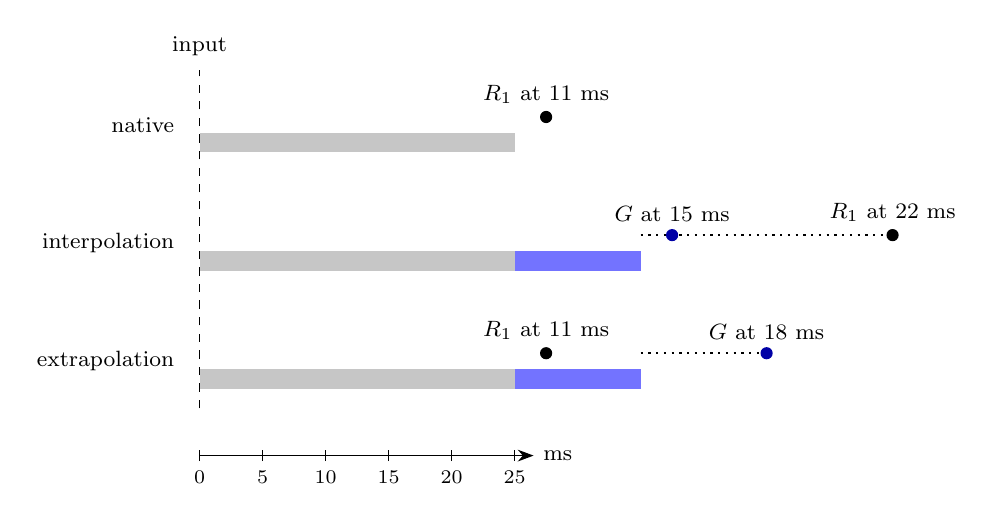
\begin{tikzpicture}[x=0.4cm, y=1cm, font=\footnotesize]
  \node[anchor=east] at (-0.5,3) {native};
  \node[anchor=east] at (-0.5,1.5) {interpolation};
  \node[anchor=east] at (-0.5,0) {extrapolation};
  \draw[dashed] (0,-0.6) -- (0,3.7);
  \node[anchor=south] at (0,3.75) {input};
  % native: render 0 to 10 ms, real frame shown at 11 ms
  \fill[gray!45] (0,2.65) rectangle (10,2.9);
  \fill[black] (11,3.1) circle (2.2pt);
  \node[anchor=south] at (11,3.15) {$R_1$ at 11 ms};
  % interpolation: render 0 to 10, generate 10 to 14, G shown at 15, R1 held and shown at 22
  \fill[gray!45] (0,1.15) rectangle (10,1.4);
  \fill[blue!55] (10,1.15) rectangle (14,1.4);
  \draw[dotted, thick] (14,1.6) -- (22,1.6);
  \fill[blue!65!black] (15,1.6) circle (2.2pt);
  \node[anchor=south] at (15,1.65) {$G$ at 15 ms};
  \fill[black] (22,1.6) circle (2.2pt);
  \node[anchor=south] at (22,1.65) {$R_1$ at 22 ms};
  % extrapolation: render 0 to 10, generate 10 to 14, R1 shown at 11, G shown at 18
  \fill[gray!45] (0,-0.35) rectangle (10,-0.1);
  \fill[blue!55] (10,-0.35) rectangle (14,-0.1);
  \fill[black] (11,0.1) circle (2.2pt);
  \node[anchor=south] at (11,0.15) {$R_1$ at 11 ms};
  \draw[dotted, thick] (14,0.1) -- (18,0.1);
  \fill[blue!65!black] (18,0.1) circle (2.2pt);
  \node[anchor=south] at (18,0.15) {$G$ at 18 ms};
  % time axis
  \draw[-{Stealth[length=2mm]}] (0,-1.2) -- (10.6,-1.2) node[right] {ms};
  \foreach \t in {0,5,10,15,20,25}{
    \draw (\t*0.4,-1.27) -- (\t*0.4,-1.13);
    \node[below, font=\scriptsize] at (\t*0.4,-1.27) {\t};
  }
\end{tikzpicture}
\caption{Schematic presentation times for one real frame and one generated frame, from the rules of the frame-pacing simulator, with render 10 ms, generation 4 ms and presentation 1 ms, and with CPU work and upscaling omitted. Grey bars are rendering, blue bars are generation and dotted lines are frames held for presentation. Interpolation holds the real frame until the generated frame is shown, so the real frame arrives 11 ms after its native time. The values are illustrative and are not measurements.}\label{fig:bg-pacing}
\end{figure}

The simulator's rules for the three modes are these. For a real frame, native latency is $c+r+s+p$, and interpolation adds $g+P/2$ to it. Extrapolation leaves it unchanged. For a generated frame, the camera latency, the time from input to the first displayed frame that reflects the camera, is $c+r+s+g+p$ for interpolation. For extrapolation it is $c+r+s+p+P/2$, or, with late latching, $g+p$.

\paragraph{Late latching.} Late latching samples the camera again as late as possible before a frame is generated, so that the generated frame moves with a newer camera. In the simulator this reduces the camera latency of an extrapolated frame to the generation time plus the presentation time, $g+p$. Late latching needs a camera input read just before generation, which the engine must provide.

\paragraph{Frame pacing and variable refresh.} Pacing means presenting frames at evenly spaced times. Uneven gaps are seen as stutter even when the mean rate is high, so the measure is the coefficient of variation of the gaps between presented frames, which the simulator reports as \texttt{frame\_gap\_cv}. A variable-refresh display presents each frame when it is ready within its supported range instead of at fixed intervals. The presentation time then equals the completion time, so irregular completion becomes irregular spacing unless the scheduler paces the frames. The simulator models such a display, which presents at the ready time.

\subsection{Metrics}\label{sec:bg-metrics}

Each metric compares an output frame $o$ with a reference frame $g$, both encoded RGB, and the references are exact because the test data are synthetic or come with ground truth. Metrics are computed per frame and per sample and then averaged. \Cref{tab:bg-metrics} summarises the direction and the limits of each measure, and the paragraphs below give the definitions exactly as the code computes them.

\begin{table}[!htbp]
\caption{Metrics of the supplement: range, direction and what each measure misses. Ranges are those of the definitions, and the cap of PSNR is the code's clamp}\label{tab:bg-metrics}
\begin{tabular*}{\columnwidth}{@{\extracolsep\fill}p{0.25\columnwidth}p{0.16\columnwidth}p{0.12\columnwidth}p{0.33\columnwidth}}
\toprule
Metric & Range & Better & What it misses \\
\midrule
PSNR (RGB, frame generation) & up to 100 dB & higher & Only the per-pixel squared error, so a blurred frame can score well \\
PSNR-Y (temporal super-resolution) & up to 100 dB & higher & Luma only, so chroma errors are ignored \\
SSIM & $-1$ to $1$ & higher & Local structure in $11\times11$ windows, nothing over time \\
LPIPS & non-negative & lower & Learned features of one network, nothing over time \\
FLIP (mean) & 0 to 1 & lower & A perceptual model with fixed viewing assumptions \\
IE & 0 to 255 & lower & A global error, like PSNR on another scale \\
Temporal-change error & non-negative & lower & Static errors that do not change in time, and it needs motion labels \\
Warp error & non-negative & lower & Agreement with the reference, so a consistently blurred output can score well \\
tOF & pixels & lower & Errors of the flow estimator, computed on every fourth frame \\
UI ghosting rate & 0 to 1 & lower & Errors below 10 percent of full scale and UI pixels only \\
Region PSNR & up to 100 dB & higher & Pixels outside the region, and the quality of the region mask \\
Gated share & 0 to 1 & lower on cut-free clips & Cuts that the gate misses, since the clips contain none \\
\botrule
\end{tabular*}
\end{table}

\paragraph{PSNR.} With a mask $M(\mathbf p)\in\{0,1\}$, the masked mean squared error and the PSNR in decibels are
\begin{equation}
\mathrm{MSE}_M=\frac{\sum_{\mathbf p}\sum_{c}M(\mathbf p)\big(o_c(\mathbf p)-g_c(\mathbf p)\big)^2}{\max\!\big(\sum_{\mathbf p}\sum_{c}M(\mathbf p),\,1\big)},\qquad \mathrm{PSNR}=10\log_{10}\frac{1}{\max(\mathrm{MSE}_M,\,10^{-10})},\label{eq:bg-psnr}
\end{equation}
where $c$ runs over the three channels and $M\equiv1$ gives the plain PSNR. The clamp caps the PSNR at 100 dB. Higher is better.

\paragraph{PSNR-Y.} The same formula is applied to $Y$ of Eq.~(\ref{eq:bg-luma}), after removing the $s$ outermost pixels of the high-resolution frame on each side (\texttt{psnr} with \texttt{border} $=s$). Because $Y$ is $219/255$ times the full-range luma plus a constant, the PSNR-Y of an error is $20\log_{10}(255/219)\approx1.32$ dB higher than the PSNR of the full-range luma with the same error. This offset is constant, so the differences between methods are unaffected.

\paragraph{SSIM.} The structural similarity index of \cite{wang2004ssim} compares local means, variances and covariance under a Gaussian window,
\begin{equation}
\mathrm{SSIM}(\mathbf p)=\frac{(2\mu_o\mu_g+C_1)(2\sigma_{og}+C_2)}{(\mu_o^2+\mu_g^2+C_1)(\sigma_o^2+\sigma_g^2+C_2)},\qquad C_1=(0.01)^2,\quad C_2=(0.03)^2,\label{eq:bg-ssim}
\end{equation}
where $\mu$, $\sigma^2$ and $\sigma_{og}$ are the local mean, variance and covariance under an $11\times11$ Gaussian window with $\sigma=1.5$ whose weights sum to one. The window is evaluated only where it lies inside the image (a valid convolution), so the map is 10 pixels smaller in each direction. The score is the mean over the map and over channels, lies in $[-1,1]$ and is higher for a better match. The temporal super-resolution network scores $Y$, and the frame generator scores each RGB channel.

\paragraph{LPIPS.} The learned perceptual distance \cite{zhang2018lpips} is
\begin{equation}
d_{\text{LPIPS}}(o,g)=\sum_{l}\frac{1}{H_lW_l}\sum_{h,w}\big\|\mathbf w_l\odot\big(\hat\phi^l_{hw}(o)-\hat\phi^l_{hw}(g)\big)\big\|_2^2,\label{eq:bg-lpips}
\end{equation}
where $\hat\phi^l_{hw}$ is the unit-normalised feature vector of AlexNet layer $l$ at position $(h,w)$, $\mathbf w_l$ are learned per-channel weights and $H_l\times W_l$ is the layer's size. Lower is better. The code calls the \texttt{lpips} package with AlexNet and \texttt{normalize=True}. If that package cannot build the network, \texttt{LPIPSAlex} builds the same network from torchvision's ImageNet AlexNet weights and the version 0.1 linear weights of the package, and maps the inputs from $[0,1]$ to $[-1,1]$ with $2x-1$ (\texttt{load\_lpips}). The temporal super-resolution evaluation computes LPIPS on every fourth frame, and the frame generator computes it on every sample.

\paragraph{FLIP.} FLIP \cite{andersson2020flip} is a perceptual difference evaluator that produces a per-pixel error map. The code calls \texttt{flip\_evaluator.evaluate} with the LDR traits and takes element 1 of its result (\texttt{flip\_error}). The official example of the package unpacks the result as the error map, the mean FLIP error and the parameters, so element 1 is the mean error. The traits string in the official example is \texttt{"HDR"}, so the LDR setting used by the code is not checked against an example here. The temporal super-resolution notebook calls the function on one frame pair, and FLIP is therefore a single-frame measure in this supplement. Lower is better.

\paragraph{Interpolation error (IE).} The code computes
\begin{equation}
\mathrm{IE}=255\sqrt{\frac{1}{3HW}\sum_{\mathbf p}\sum_{c}\big(o_c(\mathbf p)-g_c(\mathbf p)\big)^2},\label{eq:bg-ie}
\end{equation}
which is the root-mean-square difference on the 0 to 255 scale (\texttt{interpolation\_error}). Lower is better. The measure of Baker et al.\ \cite{baker2011middlebury} is the root-mean-square difference between the ground-truth and the interpolated image, taken over the RGB channels of every pixel for colour, and the 0 to 255 scale is this code's convention. \texttt{fg\_metrics} computes IE for every frame-generation sample, and the Middlebury interpolation set \cite{baker2011middlebury} is one of the frame-generation suites, with the code naming the measure after that benchmark.

\paragraph{Temporal-change error.} This measure compares the frame-to-frame change of the output with that of the reference along the reference motion. Let $m_t$ be the motion vector of frame $t$ and $v_t$ the validity mask. Define $D_o=o_t-\mathcal W(o_{t-1},m_t)$ and $D_g=g_t-\mathcal W(g_{t-1},m_t)$. The error is
\begin{equation}
e_{\text{tc}}(t)=\frac{\sum_{\mathbf p}v_t(\mathbf p)\,\tfrac13\sum_c\big|D_o(\mathbf p,c)-D_g(\mathbf p,c)\big|}{\max\big(\sum_{\mathbf p}v_t(\mathbf p),\,1\big)}.\label{eq:bg-tce}
\end{equation}
It is computed for frames $t\ge1$ of samples whose motion labels are exact or from RAFT (\texttt{temporal\_change\_error}). Lower is better. Flicker and ghosting appear as change where the reference has none, and the reference's own change is subtracted. A stable output with a constant error relative to the reference scores zero, so the measure does not see static errors. Its value also depends on the quality of the motion labels, which are less reliable for RAFT labels than for exact ones.

\paragraph{Warp error.} The warp error uses the same warp but compares the output with itself,
\begin{equation}
e_{w}(t)=\frac{\sum_{\mathbf p}v_t(\mathbf p)\,\tfrac13\sum_c\big|o_t(\mathbf p,c)-\mathcal W(o_{t-1},m_t)(\mathbf p,c)\big|}{\max\big(\sum_{\mathbf p}v_t(\mathbf p),\,1\big)},\label{eq:bg-we}
\end{equation}
and it is computed only for samples with exact motion labels (\texttt{warping\_error}). Lower is better. It measures the consistency of the output along true motion and does not look at the reference, so a consistently blurred output can score well. It should be read together with the temporal-change error.

\paragraph{tOF.} The temporal optical-flow difference of \cite{chu2020tecogan} compares the RAFT-Small flow of the output with the flow of the reference,
\begin{equation}
\mathrm{tOF}(t)=\frac{1}{HW}\sum_{\mathbf p}\big\|F^{\text{RAFT}}_{o_t\to o_{t-1}}(\mathbf p)-F^{\text{RAFT}}_{g_t\to g_{t-1}}(\mathbf p)\big\|_2,\label{eq:bg-tof}
\end{equation}
in pixels (\texttt{tof}). It is computed for $t\ge1$ with $t$ divisible by 4 (the \texttt{lpips\_every} setting). Lower is better. Flicker changes the estimated flow, so the measure detects it, but errors of RAFT itself enter both terms and cannot be separated from the output's errors. The file also defines \texttt{tlp}, the LPIPS analogue of tOF, but no evaluation function calls it, so it is not reported.

\paragraph{UI ghosting rate.} Let $U=\{\mathbf p: M_{\text{UI}}(\mathbf p)>0.5\}$, where $M_{\text{UI}}=\max(\alpha_0,\alpha_1)$ combines the UI coverage of the two real frames. The ghosting rate is
\begin{equation}
R_{\text{ghost}}=\frac{\big|\{\mathbf p\in U:\ \max_c|o_c(\mathbf p)-g_c(\mathbf p)|>0.1\}\big|}{\max(|U|,1)},\label{eq:bg-ghost}
\end{equation}
which is the share of UI pixels whose error exceeds 10 percent of full scale in any channel (\texttt{fg\_metrics}). It is defined only for samples that contain UI. Lower is better. It counts errors above the threshold and ignores their size.

\paragraph{Region PSNR.} Eq.~(\ref{eq:bg-psnr}) is restricted to five masks. The disocclusion mask is $1-v_t$ for $t\ge1$. The detail mask is the top 15 percent of the reference luma gradient, where the central differences $\partial_xY(\mathbf p)=Y(\mathbf p+\mathbf e_x)-Y(\mathbf p-\mathbf e_x)$ and $\partial_yY$ give a magnitude $\sqrt{\partial_x Y^2+\partial_y Y^2}$, thresholded at the 85th percentile of each frame (\texttt{hf\_mask}). The particle mask is the reactive mask, upsampled to output resolution and thresholded at 0.1. The UI mask is $U$. The occluded mask of the frame generator is $1-v_{\tau\to1}$, the target pixels that are not visible in $I_1$. Each region PSNR is reported only when its mask covers more than 50 pixels. Higher is better. The measure ignores all pixels outside its mask, and the disocclusion mask is only as good as the validity labels. Where a sample has no motion labels, $v$ is zero and the disocclusion mask covers the whole frame (\texttt{sr\_frame\_metrics}). When RAFT is available, every frame after the first of a real clip has labels, so the all-pixel case arises only without RAFT.

\paragraph{Gated share.} The cut gate skips generation and repeats the newest real frame where the score of Eq.~(\ref{eq:bg-cut}), with the motion term when a motion vector is available, exceeds its threshold (\texttt{cut\_gate}). The test clips contain no cuts, so every gated real sample is a false alarm, and the gated share is the fraction of real samples on which the gate fires. Lower is better on cut-free clips. The gated share says nothing about cuts that the gate misses, because the clips contain none.

\section{Data, copy detection and leakage control}\label{sec:data}

The data pipeline notebook builds the single manifest that both training notebooks read. It has three jobs. It gathers public stills and video sequences, it removes near copies so that no test content reaches training, and it records for every item its leakage group, its split and the locations of its frames, motion and depth. \cref{M-sec:data} of the article summarises the procedure. This section gives the complete method, every threshold, and every saved output of the notebook.

Every result here comes from one saved run of the pipeline. A result that rests on one run carries the \Preliminary{} tag, because a run with other seeds or other caps can change the counts. Descriptions of what the code does carry no tag. Every count and threshold quoted in this section is a generated result key, except for design constants that are written in the code, and each of these is quoted from the code.

Four terms are used throughout. An \emph{item} is one still image or one video sequence, and it is the unit of the manifest. A \emph{keyframe} is a decoded frame of an item that is used for statistics and copy detection. A \emph{leakage group} is a set of items that must never be split between training, validation and test, such as the frames of one video or one rendered scene. A \emph{duplicate edge} joins two keyframes that show the same picture. Each item ends with one split: train, val or test for items that are used, drop for an item removed because it is a near copy of test content or shares a group with it, and filtered for an item removed by a quality rule.

The notebook runs eleven timed stages in this order: Kaggle discovery, Hugging Face materialisation, keyframe statistics, quality filters, perceptual hashes, DINOv2 embeddings, SIFT features, threshold calibration, candidate search and verification, the leakage-safe split with its audit, and the manifest with the dataset card. \cref{tab:data-stages} gives the time of each stage.

\begin{table}[!htbp]
\caption{Stage times of the saved run, in minutes}\label{tab:data-stages}
\footnotesize
\begin{tabular}{@{}lr@{}}
\toprule
Stage & Minutes \\
\midrule
Kaggle discovery & \Res{data.stage_times.kaggle_discovery.minutes} \\
Hugging Face materialisation & \Res{data.stage_times.hf_materialisation.minutes} \\
Keyframe statistics & \Res{data.stage_times.keyframe_stats.minutes} \\
Filters & \Res{data.stage_times.filters.minutes} \\
Perceptual hashes & \Res{data.stage_times.hashes.minutes} \\
Embeddings & \Res{data.stage_times.embeddings.minutes} \\
Local features (SIFT) & \Res{data.stage_times.local_features.minutes} \\
Calibration & \Res{data.stage_times.calibration.minutes} \\
Duplicate search and verification & \Res{data.stage_times.duplicate_search.minutes} \\
Split and audit & \Res{data.stage_times.split_and_audit.minutes} \\
Manifest & \Res{data.stage_times.manifest.minutes} \\
\bottomrule
\end{tabular}
\end{table}

\subsection{Source datasets}\label{sec:data-sources}

The pipeline reads two hosts. The Kaggle datasets are attached to the notebook and read from the read-only input mount, which the code locates by the dataset's owner and slug. The Hugging Face (HF) datasets are read over HTTPS. The code keeps one connection alive per thread, checks the length of every range read, and retries failed reads. A zip member is read through range requests without downloading the archive, and the GameIR tars are read as one sequential stream that stops once the clip cap is reached. The Vimeo-1080p step is different. It downloads each named parquet shard in full, reads the MP4 files inside it, and deletes the shard, so the notebook's statement that the pipeline makes no full archive downloads does not hold for that source. Each source is optional. A source that fails is logged and skipped, and the run continues.

\Cref{tab:data-sources} lists the eleven sources. The sizes are the means of the saved keyframe sizes. The licence column repeats the strings written in the code. The upstream licence pages were not checked for this section, so these are the code's statements and not checked legal facts. The code marks the game captures as needing a check for each use, and it gives the Vimeo-1080p licence as unspecified. The notebook's dataset card refers to \texttt{RESEARCH.md} for commercial-use restrictions. That file exists in the repository, but its contents were not checked for this section. The licences need checking against each upstream page before any release.

\begin{table}[!htbp]
\caption{Source datasets, as the code reads them. Sizes are mean keyframe widths and heights in pixels from the saved keyframe table. Licence strings are the code's statements, not checked against upstream pages}\label{tab:data-sources}
\footnotesize
\begin{tabular}{@{}p{2.4cm}p{3.2cm}p{3.6cm}p{1.9cm}@{}}
\toprule
Source & Host and identifier & Content and ground truth & Size (px) \\
\midrule
DIV2K & Kaggle \texttt{soumikrakshit/\allowbreak div2k-\allowbreak high-\allowbreak resolution-\allowbreak images} & Photographs, still, no motion, and validation images pinned to test & \Res{data.keyframe_stats.div2k.width.mean}$\times$\Res{data.keyframe_stats.div2k.height.mean} \\
Flickr2K & Kaggle \texttt{daehoyang/flickr2k} & Photographs, still, train only & \Res{data.keyframe_stats.flickr2k.width.mean}$\times$\Res{data.keyframe_stats.flickr2k.height.mean} \\
Game stills & HF \texttt{ericphann/\allowbreak video-\allowbreak game-\allowbreak super-\allowbreak resolution} & 1080p game captures, still, with \texttt{training-hr} as train and \texttt{test-hr} as test & \Res{data.keyframe_stats.game_stills.width.mean}$\times$\Res{data.keyframe_stats.game_stills.height.mean} \\
REDS & Kaggle \texttt{amithkesavmrajagiri/\allowbreak reds-\allowbreak dataset} & 720p video clips, no motion labels, train only & \Res{data.keyframe_stats.reds.width.mean}$\times$\Res{data.keyframe_stats.reds.height.mean} \\
Vimeo-90K septuplets & Kaggle \texttt{wangsally/\allowbreak vimeo-\allowbreak 90k-\allowbreak 7} & Seven-frame video sequences, no motion labels, train only & \Res{data.keyframe_stats.vimeo_septuplet.width.mean}$\times$\Res{data.keyframe_stats.vimeo_septuplet.height.mean} \\
Vimeo-90K triplets & Kaggle \texttt{chenshu123/\allowbreak vimeo-\allowbreak triplet} & Three-frame sequences from the official test list, test only & \Res{data.keyframe_stats.vimeo_triplet.width.mean}$\times$\Res{data.keyframe_stats.vimeo_triplet.height.mean} \\
MPI Sintel & Kaggle \texttt{artemmmtry/\allowbreak mpi-\allowbreak sintel-\allowbreak dataset} & Rendered scenes with exact forward flow and occlusion masks, with \texttt{market} and \texttt{cave} as test & \Res{data.keyframe_stats.sintel.width.mean}$\times$\Res{data.keyframe_stats.sintel.height.mean} \\
Vid4 & Kaggle \texttt{uom200647r/\allowbreak vid4-\allowbreak dataset} & Video clips, no motion labels, test only & \Res{data.keyframe_stats.vid4.width.mean}$\times$\Res{data.keyframe_stats.vid4.height.mean} \\
TartanAir & HF \texttt{theairlabcmu/tartanair} & Rendered scenes with exact forward flow, occlusion masks and depth, with two environments as test & \Res{data.keyframe_stats.tartanair.width.mean}$\times$\Res{data.keyframe_stats.tartanair.height.mean} \\
GameIR & HF \texttt{LLLebin/GameIR} & CARLA and Unreal Engine 4 game renders at 1440p and 720p, with depth and no exact flow, and the test tar as test & \Res{data.keyframe_stats.gameir.width.mean}$\times$\Res{data.keyframe_stats.gameir.height.mean} \\
Vimeo-1080p & HF \texttt{danjacobellis/\allowbreak vimeo1080p} & 1080p MP4 videos, no motion labels, validation shard as test & \Res{data.keyframe_stats.vimeo1080p.width.mean}$\times$\Res{data.keyframe_stats.vimeo1080p.height.mean} \\
\bottomrule
\end{tabular}
\end{table}

The roles are set by the code. The test items are the DIV2K validation images, the Vid4 clips, the official Vimeo-90K triplet test list, the Sintel \texttt{market} and \texttt{cave} scene families, the two TartanAir test environments, the GameIR test tar and the Vimeo-1080p validation shard. Every other item is a training candidate, and the split of \cref{sec:data-split} decides whether it ends in train or val. The sources are DIV2K \cite{agustsson2017div2k}, REDS \cite{nah2019reds}, Vimeo-90K \cite{xue2019vimeo}, MPI Sintel \cite{butler2012sintel}, TartanAir \cite{wang2020tartanair}, GameIR \cite{zhou2024gameir}, Vid4 \cite{liu2014vid4} and CARLA \cite{dosovitskiy2017carla}, which the GameIR renders use. The DIV2K training and validation counts follow the published split of 800 training and 100 validation images, which the catalogue reproduces.

Two sources carry ground truth beyond the frames themselves. Sintel and TartanAir give exact forward optical flow and occlusion masks, and TartanAir and GameIR give depth. These are the only sources the training uses as exact labels, and the rest rely on the frames, either as targets or through the RAFT teacher flow of \cref{sec:data-synth-tsr}.

\subsection{Discovery and catalogue}\label{sec:data-discovery}

Discovery runs once per attached Kaggle dataset, and the seven Kaggle sources run in parallel threads. For each dataset the code lists files with \texttt{sampled\_walk}. This function keeps a frontier of directories, expands one directory chosen at random at each step, and lists every file in that directory completely. A listed sequence folder is therefore never cut in half. Listing stops when the file cap is reached, which is \Res{data.config.cfg.list_cap_files} files by default. The REDS and Vimeo-90K septuplet listings reached the cap before the walk finished, so their listings are incomplete, and the other sources listed completely.

A file is kept only if its path has no token that marks a degraded copy or a non-colour pass. The degraded tokens are \texttt{lr}, \texttt{lq}, \texttt{bicubic}, \texttt{blur}, \texttt{x2} to \texttt{x4} and similar, and the non-colour tokens include \texttt{flow}, \texttt{depth}, \texttt{occlusions}, \texttt{mask} and \texttt{albedo}. Tokens are the lower-case pieces of the directory and file names. For video, if any path carries a high-resolution token (\texttt{hr}, \texttt{gt}, \texttt{original} or \texttt{groundtruth}), only those paths are kept. Stills become one item each. Video frames become one item per folder, and the leakage group is the folder name for level 1 sources and the parent folder for level 2 sources. A folder with fewer than three frames is skipped. For Sintel, the group is the scene prefix (for example \texttt{market}), and each item carries the forward flow files and the occlusion masks that match its frames. The Vimeo-90K triplet clips are read directly from the official test list, and up to 1,000 of them are sampled with the seed.

\Cref{tab:data-discovery} reports the discovery per source. The listed and kept counts are file counts, and the items are the sequences or stills that survived the path rules. Sintel lists \Res{data.discovery_kaggle.sintel.listed} files and keeps \Res{data.discovery_kaggle.sintel.kept_files} of them, and the difference comes from files that the path rules remove, such as non-colour passes and masks. \Preliminary

\begin{table}[!htbp]
\caption{Kaggle discovery per source. Files are counted after the directory walk and after the path rules. The REDS and Vimeo-90K septuplet listings reached their cap, so their file counts are lower bounds}\label{tab:data-discovery}
\footnotesize
\begin{tabular}{@{}lrrrrr@{}}
\toprule
Source & Files listed & Files kept & Directories listed & Items & Test items \\
\midrule
DIV2K & \Res{data.discovery_kaggle.div2k.listed} & \Res{data.discovery_kaggle.div2k.kept_files} & \Res{data.discovery_kaggle.div2k.dirs_listed} & \Res{data.discovery_kaggle.div2k.items} & \Res{data.discovery_kaggle.div2k.test_items} \\
Flickr2K & \Res{data.discovery_kaggle.flickr2k.listed} & \Res{data.discovery_kaggle.flickr2k.kept_files} & \Res{data.discovery_kaggle.flickr2k.dirs_listed} & \Res{data.discovery_kaggle.flickr2k.items} & \Res{data.discovery_kaggle.flickr2k.test_items} \\
REDS & \Res{data.discovery_kaggle.reds.listed} & \Res{data.discovery_kaggle.reds.kept_files} & \Res{data.discovery_kaggle.reds.dirs_listed} & \Res{data.discovery_kaggle.reds.items} & \Res{data.discovery_kaggle.reds.test_items} \\
Vimeo-90K septuplets & \Res{data.discovery_kaggle.vimeo_septuplet.listed} & \Res{data.discovery_kaggle.vimeo_septuplet.kept_files} & \Res{data.discovery_kaggle.vimeo_septuplet.dirs_listed} & \Res{data.discovery_kaggle.vimeo_septuplet.items} & \Res{data.discovery_kaggle.vimeo_septuplet.test_items} \\
Vimeo-90K triplets & \Res{data.discovery_kaggle.vimeo_triplet.listed} & \Res{data.discovery_kaggle.vimeo_triplet.kept_files} & \Res{data.discovery_kaggle.vimeo_triplet.dirs_listed} & \Res{data.discovery_kaggle.vimeo_triplet.items} & \Res{data.discovery_kaggle.vimeo_triplet.test_items} \\
MPI Sintel & \Res{data.discovery_kaggle.sintel.listed} & \Res{data.discovery_kaggle.sintel.kept_files} & \Res{data.discovery_kaggle.sintel.dirs_listed} & \Res{data.discovery_kaggle.sintel.items} & \Res{data.discovery_kaggle.sintel.test_items} \\
Vid4 & \Res{data.discovery_kaggle.vid4.listed} & \Res{data.discovery_kaggle.vid4.kept_files} & \Res{data.discovery_kaggle.vid4.dirs_listed} & \Res{data.discovery_kaggle.vid4.items} & \Res{data.discovery_kaggle.vid4.test_items} \\
\bottomrule
\end{tabular}
\end{table}

The Hugging Face sources are materialised next, into the data root, and each one follows its own access rule. Game stills are a random sample of the listed PNG files in the training and test folders, with the seed. TartanAir is read per environment. For each environment the code reads the first trajectory of the Easy difficulty zips, takes a contiguous run of frames starting at one quarter of the way along the trajectory, and stores RGB, depth, forward flow and a validity mask. The validity mask is white where the TartanAir mask is zero, which means a valid correspondence. The run stops early if a flow or mask file is missing. Each run is cut into sequences of 24 frames, which is the TartanAir sequence length in the configuration. GameIR keeps the 1440p and 720p renders and the depth of every clip with at least three high-resolution frames and a matching low-resolution frame. The code records a frame stride of ten rendered frames for these clips, but it does not subsample them, so the frames are whatever the mini tar holds. Vimeo-1080p writes each MP4 to disk, counts its frames, and keeps videos with at least eight frames.

\Cref{tab:data-catalogue} is the catalogue, which counts items, frames, exact-motion items and depth items for each source and role. The counts are taken before the quality filters, so they describe what was materialised. \Preliminary

\begin{table}[!htbp]
\caption{Catalogue before filtering, by source, kind and role. Exact motion counts items with exact forward flow and depth counts items with depth. Each row is one source and role that exists in the run}\label{tab:data-catalogue}
\footnotesize
\begin{tabular}{@{}llrrrrr@{}}
\toprule
Source & Role & Items & Frames & Exact motion & Depth \\
\midrule
DIV2K & train & \Res{data.catalogue_summary.div2k.still.train.items} & \Res{data.catalogue_summary.div2k.still.train.frames} & \Res{data.catalogue_summary.div2k.still.train.exact_motion} & \Res{data.catalogue_summary.div2k.still.train.with_depth} \\
DIV2K & test & \Res{data.catalogue_summary.div2k.still.test.items} & \Res{data.catalogue_summary.div2k.still.test.frames} & \Res{data.catalogue_summary.div2k.still.test.exact_motion} & \Res{data.catalogue_summary.div2k.still.test.with_depth} \\
Flickr2K & train & \Res{data.catalogue_summary.flickr2k.still.train.items} & \Res{data.catalogue_summary.flickr2k.still.train.frames} & \Res{data.catalogue_summary.flickr2k.still.train.exact_motion} & \Res{data.catalogue_summary.flickr2k.still.train.with_depth} \\
Game stills & train & \Res{data.catalogue_summary.game_stills.still.train.items} & \Res{data.catalogue_summary.game_stills.still.train.frames} & \Res{data.catalogue_summary.game_stills.still.train.exact_motion} & \Res{data.catalogue_summary.game_stills.still.train.with_depth} \\
Game stills & test & \Res{data.catalogue_summary.game_stills.still.test.items} & \Res{data.catalogue_summary.game_stills.still.test.frames} & \Res{data.catalogue_summary.game_stills.still.test.exact_motion} & \Res{data.catalogue_summary.game_stills.still.test.with_depth} \\
GameIR & train & \Res{data.catalogue_summary.gameir.seq.train.items} & \Res{data.catalogue_summary.gameir.seq.train.frames} & \Res{data.catalogue_summary.gameir.seq.train.exact_motion} & \Res{data.catalogue_summary.gameir.seq.train.with_depth} \\
GameIR & test & \Res{data.catalogue_summary.gameir.seq.test.items} & \Res{data.catalogue_summary.gameir.seq.test.frames} & \Res{data.catalogue_summary.gameir.seq.test.exact_motion} & \Res{data.catalogue_summary.gameir.seq.test.with_depth} \\
REDS & train & \Res{data.catalogue_summary.reds.seq.train.items} & \Res{data.catalogue_summary.reds.seq.train.frames} & \Res{data.catalogue_summary.reds.seq.train.exact_motion} & \Res{data.catalogue_summary.reds.seq.train.with_depth} \\
Vimeo-90K septuplets & train & \Res{data.catalogue_summary.vimeo_septuplet.seq.train.items} & \Res{data.catalogue_summary.vimeo_septuplet.seq.train.frames} & \Res{data.catalogue_summary.vimeo_septuplet.seq.train.exact_motion} & \Res{data.catalogue_summary.vimeo_septuplet.seq.train.with_depth} \\
Vimeo-90K triplets & test & \Res{data.catalogue_summary.vimeo_triplet.seq.test.items} & \Res{data.catalogue_summary.vimeo_triplet.seq.test.frames} & \Res{data.catalogue_summary.vimeo_triplet.seq.test.exact_motion} & \Res{data.catalogue_summary.vimeo_triplet.seq.test.with_depth} \\
MPI Sintel & train & \Res{data.catalogue_summary.sintel.seq.train.items} & \Res{data.catalogue_summary.sintel.seq.train.frames} & \Res{data.catalogue_summary.sintel.seq.train.exact_motion} & \Res{data.catalogue_summary.sintel.seq.train.with_depth} \\
MPI Sintel & test & \Res{data.catalogue_summary.sintel.seq.test.items} & \Res{data.catalogue_summary.sintel.seq.test.frames} & \Res{data.catalogue_summary.sintel.seq.test.exact_motion} & \Res{data.catalogue_summary.sintel.seq.test.with_depth} \\
TartanAir & train & \Res{data.catalogue_summary.tartanair.seq.train.items} & \Res{data.catalogue_summary.tartanair.seq.train.frames} & \Res{data.catalogue_summary.tartanair.seq.train.exact_motion} & \Res{data.catalogue_summary.tartanair.seq.train.with_depth} \\
TartanAir & test & \Res{data.catalogue_summary.tartanair.seq.test.items} & \Res{data.catalogue_summary.tartanair.seq.test.frames} & \Res{data.catalogue_summary.tartanair.seq.test.exact_motion} & \Res{data.catalogue_summary.tartanair.seq.test.with_depth} \\
Vid4 & test & \Res{data.catalogue_summary.vid4.seq.test.items} & \Res{data.catalogue_summary.vid4.seq.test.frames} & \Res{data.catalogue_summary.vid4.seq.test.exact_motion} & \Res{data.catalogue_summary.vid4.seq.test.with_depth} \\
Vimeo-1080p & train & \Res{data.catalogue_summary.vimeo1080p.seq.train.items} & \Res{data.catalogue_summary.vimeo1080p.seq.train.frames} & \Res{data.catalogue_summary.vimeo1080p.seq.train.exact_motion} & \Res{data.catalogue_summary.vimeo1080p.seq.train.with_depth} \\
Vimeo-1080p & test & \Res{data.catalogue_summary.vimeo1080p.seq.test.items} & \Res{data.catalogue_summary.vimeo1080p.seq.test.frames} & \Res{data.catalogue_summary.vimeo1080p.seq.test.exact_motion} & \Res{data.catalogue_summary.vimeo1080p.seq.test.with_depth} \\
\bottomrule
\end{tabular}
\end{table}

\Cref{fig:data-catalogue} shows the same catalogue as plots. The left panel stacks the items of each source by role. The Vimeo-90K septuplets are the largest source by items, and the Vimeo-90K triplets, which are test only, form the largest block of test items. The right panel gives the frame totals on a logarithmic axis, which spans about three decades. The Vimeo-90K and Vimeo-1080p sources carry the most frames, and the sources with exact motion and depth are a small share of the frames. \Observation

\begin{figure}[!htbp]
\centering
\includegraphics[width=0.9\textwidth]{\DataOut/plots/catalogue.png}
\caption{Catalogue before filtering. Left: items per source, stacked by role. Right: frames on a logarithmic axis, and the sequences with exact motion and with depth. Both panels come from the notebook's catalogue cell}\label{fig:data-catalogue}
\end{figure}

\subsection{Quality filtering}\label{sec:data-filters}

Quality is judged on statistics of the keyframes, which \cref{sec:data-keyframes} defines. For each keyframe the code computes the grey mean and the grey standard deviation of the full-resolution frame, where grey is the mean of the red, green and blue values. It also computes the letterbox fraction $\lambda$. A row counts as dark when its mean grey value is below 8. The letterbox fraction is the number of dark rows at the top plus the number at the bottom, divided by the frame height. The sharpness is computed on the 256 by 256 thumbnail $g$. The code applies the four-neighbour Laplacian
\begin{equation}
L(x,y)=4g(x,y)-g(x-1,y)-g(x+1,y)-g(x,y-1)-g(x,y+1),\label{eq:data-sharp}
\end{equation}
and takes the variance of $L$ over the interior pixels as the sharpness. A flat image has a small variance of $L$, and a sharp image has a large one. The colourfulness measure of each keyframe uses the opponent channels $rg=R-G$ and $yb=\tfrac{1}{2}(R+G)-B$, and its value is
\begin{equation}
C=\sqrt{\sigma_{rg}^2+\sigma_{yb}^2}+0.3\sqrt{\mu_{rg}^2+\mu_{yb}^2},\label{eq:data-colour}
\end{equation}
where $\sigma$ and $\mu$ are the standard deviation and mean over the thumbnail. This is the colourfulness index of Hasler and S{\"u}sstrunk \cite{hasler2003measuring}. The colourfulness is recorded but no rule uses it.

An item is rejected if it has any of five reasons. The first is a decode error, which means a keyframe could not be read. The second is a side below 256 pixels, which means any keyframe with a smaller width or height than 256. The third is flatness, which means the median grey standard deviation over the item's keyframes is below 8. The fourth is letterboxing, which means the median letterbox fraction is above 0.35. The fifth is blur, which means the median sharpness is below 20 for stills and below 5 for sequences. Stills are judged on their one keyframe. Sequences are judged on the median of their keyframes, so one dark shot or one fade does not reject a whole video. A rejected item keeps its row in the manifest with split filtered and is left out of the duplicate search, so the decision can be audited. The manifest does not record which rule fired. The notebook printed these reasons, but the printed output was not saved, so this section gives no per-reason counts.

\Cref{tab:data-split-source} gives the per-source totals. In this run \Res{data.summary.filtered} of \Res{data.summary.items} items were filtered. Filtering removed \Res{data.split_by_source.vimeo_septuplet.filtered} Vimeo-90K septuplet items and \Res{data.split_by_source.game_stills.filtered} game-still items, and the remaining filtered items came from the triplet and Vimeo-1080p sources. The filtered items are a small share of all items. \Preliminary

\begin{table}[!htbp]
\caption{Split per source. Drop means removed as a near copy of test content or as a member of a test group, and filtered means removed by a quality rule}\label{tab:data-split-source}
\footnotesize
\begin{tabular}{@{}lrrrrr@{}}
\toprule
Source & Train & Val & Test & Drop & Filtered \\
\midrule
DIV2K & \Res{data.split_by_source.div2k.train} & \Res{data.split_by_source.div2k.val} & \Res{data.split_by_source.div2k.test} & \Res{data.split_by_source.div2k.drop} & \Res{data.split_by_source.div2k.filtered} \\
Flickr2K & \Res{data.split_by_source.flickr2k.train} & \Res{data.split_by_source.flickr2k.val} & \Res{data.split_by_source.flickr2k.test} & \Res{data.split_by_source.flickr2k.drop} & \Res{data.split_by_source.flickr2k.filtered} \\
Game stills & \Res{data.split_by_source.game_stills.train} & \Res{data.split_by_source.game_stills.val} & \Res{data.split_by_source.game_stills.test} & \Res{data.split_by_source.game_stills.drop} & \Res{data.split_by_source.game_stills.filtered} \\
GameIR & \Res{data.split_by_source.gameir.train} & \Res{data.split_by_source.gameir.val} & \Res{data.split_by_source.gameir.test} & \Res{data.split_by_source.gameir.drop} & \Res{data.split_by_source.gameir.filtered} \\
REDS & \Res{data.split_by_source.reds.train} & \Res{data.split_by_source.reds.val} & \Res{data.split_by_source.reds.test} & \Res{data.split_by_source.reds.drop} & \Res{data.split_by_source.reds.filtered} \\
MPI Sintel & \Res{data.split_by_source.sintel.train} & \Res{data.split_by_source.sintel.val} & \Res{data.split_by_source.sintel.test} & \Res{data.split_by_source.sintel.drop} & \Res{data.split_by_source.sintel.filtered} \\
TartanAir & \Res{data.split_by_source.tartanair.train} & \Res{data.split_by_source.tartanair.val} & \Res{data.split_by_source.tartanair.test} & \Res{data.split_by_source.tartanair.drop} & \Res{data.split_by_source.tartanair.filtered} \\
Vid4 & \Res{data.split_by_source.vid4.train} & \Res{data.split_by_source.vid4.val} & \Res{data.split_by_source.vid4.test} & \Res{data.split_by_source.vid4.drop} & \Res{data.split_by_source.vid4.filtered} \\
Vimeo-1080p & \Res{data.split_by_source.vimeo1080p.train} & \Res{data.split_by_source.vimeo1080p.val} & \Res{data.split_by_source.vimeo1080p.test} & \Res{data.split_by_source.vimeo1080p.drop} & \Res{data.split_by_source.vimeo1080p.filtered} \\
Vimeo-90K septuplets & \Res{data.split_by_source.vimeo_septuplet.train} & \Res{data.split_by_source.vimeo_septuplet.val} & \Res{data.split_by_source.vimeo_septuplet.test} & \Res{data.split_by_source.vimeo_septuplet.drop} & \Res{data.split_by_source.vimeo_septuplet.filtered} \\
Vimeo-90K triplets & \Res{data.split_by_source.vimeo_triplet.train} & \Res{data.split_by_source.vimeo_triplet.val} & \Res{data.split_by_source.vimeo_triplet.test} & \Res{data.split_by_source.vimeo_triplet.drop} & \Res{data.split_by_source.vimeo_triplet.filtered} \\
\bottomrule
\end{tabular}
\end{table}

\Cref{fig:data-quality} shows the distributions that the rules act on. The grey standard deviation of the septuplet keyframes forms a bell shape centred well above the threshold of 8, so the flatness rule touches only the lower tail. The sharpness panel is on a logarithmic axis, and its two dashed lines mark the still and sequence thresholds, which are both drawn for every source. The sequences sit well above the sequence threshold, the stills sit higher still, and the sequence threshold cuts only the far lower tail. Several keyframes have a sharpness of zero, which the figure shows at the left edge. The letterbox panel is concentrated at zero, with a smaller group near 0.25 and few keyframes beyond the threshold of 0.35. \Observation

\begin{figure}[!htbp]
\centering
\includegraphics[width=0.9\textwidth]{\DataOut/plots/quality_distributions.png}
\caption{Keyframe statistics that the filters use, by source: grey standard deviation (left), log10 sharpness (centre) and letterbox fraction (right). Dashed lines mark the thresholds. The sharpness panel draws both the still and the sequence thresholds for every source}\label{fig:data-quality}
\end{figure}

\Cref{fig:data-rejected} shows the first sixteen rejected keyframes. Most are very dark. The flatness and letterbox rules reject dark frames, and the blurry examples are soft frames with little texture. The sharpness rule therefore rejects low-texture content as well as defocus, and the label blurry means low Laplacian variance. The figure is a selection, not a sample. The code takes the first two rejected keyframes of each source and reason and then keeps the first sixteen rows, so the grid shows only the Vimeo-90K septuplets, the Vimeo-90K triplets and the game stills. The notebook text describes examples from every source and reason, but the selection does not do that. \Observation

\begin{figure}[!htbp]
\centering
\includegraphics[width=0.85\textwidth]{\DataOut/plots/rejected_examples.png}
\caption{The first sixteen rejected keyframes in keyframe order, with the reasons of each item. The grid does not cover every source or reason, because the code keeps the first sixteen rows of its selection}\label{fig:data-rejected}
\end{figure}

\subsection{Keyframe selection and statistics}\label{sec:data-keyframes}

Each item is represented by keyframes, chosen from its frame list. A still and a sequence of one frame give one keyframe, which is the frame itself. A sequence of two to 23 frames gives its middle frame. A sequence of 24 or more frames gives three keyframes, at 10, 50 and 90 percent of its length, because the first and last frames of a long video are often fades or black. The triplets and septuplets are shorter than 24 frames, and so they contribute one keyframe each, while the long REDS, Vimeo-1080p and TartanAir sequences contribute three each. The total is \Res{data.summary.keyframes} keyframes for \Res{data.summary.items} items.

Each keyframe is decoded in a pool of spawned worker processes. The workers are spawned, not forked, so they do not inherit the CUDA context or the thread locks of the notebook kernel, and a dead worker raises an error instead of hanging. Each keyframe gives a 256 by 256 thumbnail, resized with bilinear filtering. The resize does not keep the aspect ratio, so a 16:9 frame is squashed horizontally and a 4:3 frame is squashed less. This is a property of the method and its effect on copy recall is not measured. The thumbnail is the input to the hashes, the embedding and the local features, and the full-resolution statistics above are computed before the resize. \Cref{tab:data-keyframes} gives the mean statistics per source. The sharpness mean is largest for Vid4 and smallest for the Vimeo-90K septuplets. Sharpness is measured on the 256 pixel thumbnail, so the value also depends on how much each source was reduced to that size, and it is not a measure of image quality across sources. \Observation

\begin{table}[!htbp]
\caption{Keyframe counts and mean statistics per source. Width and height are in pixels, grey standard deviation is on the full-resolution frame, sharpness is the Laplacian variance of the 256 by 256 thumbnail, and letterbox is the largest fraction in the source}\label{tab:data-keyframes}
\footnotesize
\begin{tabular}{@{}lrrrrrr@{}}
\toprule
Source & Keyframes & Width & Height & Grey std & Sharpness & Letterbox max \\
\midrule
DIV2K & \Res{data.keyframe_stats.div2k.n} & \Res{data.keyframe_stats.div2k.width.mean} & \Res{data.keyframe_stats.div2k.height.mean} & \Res{data.keyframe_stats.div2k.std.mean} & \Res{data.keyframe_stats.div2k.sharpness.mean} & \Res{data.keyframe_stats.div2k.letterbox.max} \\
Flickr2K & \Res{data.keyframe_stats.flickr2k.n} & \Res{data.keyframe_stats.flickr2k.width.mean} & \Res{data.keyframe_stats.flickr2k.height.mean} & \Res{data.keyframe_stats.flickr2k.std.mean} & \Res{data.keyframe_stats.flickr2k.sharpness.mean} & \Res{data.keyframe_stats.flickr2k.letterbox.max} \\
Game stills & \Res{data.keyframe_stats.game_stills.n} & \Res{data.keyframe_stats.game_stills.width.mean} & \Res{data.keyframe_stats.game_stills.height.mean} & \Res{data.keyframe_stats.game_stills.std.mean} & \Res{data.keyframe_stats.game_stills.sharpness.mean} & \Res{data.keyframe_stats.game_stills.letterbox.max} \\
GameIR & \Res{data.keyframe_stats.gameir.n} & \Res{data.keyframe_stats.gameir.width.mean} & \Res{data.keyframe_stats.gameir.height.mean} & \Res{data.keyframe_stats.gameir.std.mean} & \Res{data.keyframe_stats.gameir.sharpness.mean} & \Res{data.keyframe_stats.gameir.letterbox.max} \\
REDS & \Res{data.keyframe_stats.reds.n} & \Res{data.keyframe_stats.reds.width.mean} & \Res{data.keyframe_stats.reds.height.mean} & \Res{data.keyframe_stats.reds.std.mean} & \Res{data.keyframe_stats.reds.sharpness.mean} & \Res{data.keyframe_stats.reds.letterbox.max} \\
MPI Sintel & \Res{data.keyframe_stats.sintel.n} & \Res{data.keyframe_stats.sintel.width.mean} & \Res{data.keyframe_stats.sintel.height.mean} & \Res{data.keyframe_stats.sintel.std.mean} & \Res{data.keyframe_stats.sintel.sharpness.mean} & \Res{data.keyframe_stats.sintel.letterbox.max} \\
TartanAir & \Res{data.keyframe_stats.tartanair.n} & \Res{data.keyframe_stats.tartanair.width.mean} & \Res{data.keyframe_stats.tartanair.height.mean} & \Res{data.keyframe_stats.tartanair.std.mean} & \Res{data.keyframe_stats.tartanair.sharpness.mean} & \Res{data.keyframe_stats.tartanair.letterbox.max} \\
Vid4 & \Res{data.keyframe_stats.vid4.n} & \Res{data.keyframe_stats.vid4.width.mean} & \Res{data.keyframe_stats.vid4.height.mean} & \Res{data.keyframe_stats.vid4.std.mean} & \Res{data.keyframe_stats.vid4.sharpness.mean} & \Res{data.keyframe_stats.vid4.letterbox.max} \\
Vimeo-1080p & \Res{data.keyframe_stats.vimeo1080p.n} & \Res{data.keyframe_stats.vimeo1080p.width.mean} & \Res{data.keyframe_stats.vimeo1080p.height.mean} & \Res{data.keyframe_stats.vimeo1080p.std.mean} & \Res{data.keyframe_stats.vimeo1080p.sharpness.mean} & \Res{data.keyframe_stats.vimeo1080p.letterbox.max} \\
Vimeo-90K septuplets & \Res{data.keyframe_stats.vimeo_septuplet.n} & \Res{data.keyframe_stats.vimeo_septuplet.width.mean} & \Res{data.keyframe_stats.vimeo_septuplet.height.mean} & \Res{data.keyframe_stats.vimeo_septuplet.std.mean} & \Res{data.keyframe_stats.vimeo_septuplet.sharpness.mean} & \Res{data.keyframe_stats.vimeo_septuplet.letterbox.max} \\
Vimeo-90K triplets & \Res{data.keyframe_stats.vimeo_triplet.n} & \Res{data.keyframe_stats.vimeo_triplet.width.mean} & \Res{data.keyframe_stats.vimeo_triplet.height.mean} & \Res{data.keyframe_stats.vimeo_triplet.std.mean} & \Res{data.keyframe_stats.vimeo_triplet.sharpness.mean} & \Res{data.keyframe_stats.vimeo_triplet.letterbox.max} \\
\bottomrule
\end{tabular}
\end{table}

\subsection{Copy detection}\label{sec:data-copy}

A copy is a keyframe that shows the same picture as another keyframe, after a change of scale, compression, colour, crop or mirror. Copy detection must separate copies from similar pictures. Two photographs of the same kind of scene, two frames of one game or two skylines can be close in a global description while showing different pictures. The pipeline therefore uses a two-stage rule. The first stage proposes candidate pairs with cheap global descriptions. The second stage confirms a pair with a geometric check, and two further tests accept pairs whose global scores lie beyond every hard negative.
\paragraph{Perceptual hashes.} A perceptual hash maps an image to a short bit string that changes little under compression and scaling \cite{venkatesan2000robust}. The variant below, a DCT hash with a difference hash (dHash) alongside it, is this code's choice. The pHash of a keyframe takes its 32 by 32 grey image $G$ and computes the two-dimensional discrete cosine transform
\begin{equation}
C=D\,G\,D^{\mathsf T},\label{eq:data-phash}
\end{equation}
where $D$ is the 32 by 32 orthonormal DCT-II matrix. The 8 by 8 block of lowest frequencies is kept, and the direct-current term is left out of the median. Each of the 64 bits is one if its coefficient is above that median, and zero otherwise. The dHash takes a 9 by 8 grey image and sets each bit to one when the pixel to the right is brighter than the pixel on the left. The distance between two hashes is the Hamming distance, which counts the bits that differ. The code uses 64-bit hashes, so the distance ranges from 0 to 64. Hashes catch near-exact copies, including rescaled, recompressed and recoloured frames. They do not catch crops or mirror images, and the later stages cover those.

\paragraph{Global embeddings and cosine similarity.} The embedding uses DINOv2-small, a self-supervised vision transformer \cite{oquab2024dinov2}, and the code's descriptor for each image has 384 dimensions, as the embedding log of the data pipeline records. The code takes the pooled output of the model for each thumbnail after bilinear resizing to 224 by 224, with the usual channel means and standard deviations, and it normalises the output to unit length. For two unit vectors $u$ and $v$, the cosine similarity is $u\cdot v$, and for general vectors it is
\begin{equation}
\cos(u,v)=\frac{u\cdot v}{\lVert u\rVert\,\lVert v\rVert}.\label{eq:data-cos}
\end{equation}
A cosine near one means that the two descriptors point the same way. Two different pictures with similar content can also have a high cosine, which is why the embedding only proposes candidates. The model runs in half precision on both GPUs, in batches of 256 thumbnails.

\paragraph{Exhaustive neighbour search.} For every searched keyframe, the code finds its $k$ neighbours with the largest dot products, where $k=\Res{data.config.cfg.dedup.k}$. A neighbour must belong to a different leakage group, so a keyframe never matches its own sequence. The search computes the full similarity matrix in chunks of 2,048 rows on the GPU and takes the top $k$ of each row. Hash candidates are found in the same spirit. Each hash bit becomes $+1$ or $-1$, and two hashes have a Hamming distance $h$ exactly when the dot product of their $\pm1$ vectors is $64-2h$. The code therefore finds all pairs whose dot product passes $64-2h$, in chunks of 4,096 rows, and it looks only at textured keyframes, which are those with a grey standard deviation of at least \Res{data.config.cfg.dedup.min_std_hash}.

\paragraph{Local features and geometric verification.} The second stage looks for shared structure. The code runs the scale-invariant feature transform (SIFT) on each thumbnail and on its mirror image, keeps up to \Res{data.config.cfg.dedup.sift_features} keypoints per image, and stores their 128-dimensional descriptors \cite{lowe2004sift}. For two keyframes $A$ and $B$, a keypoint of $A$ is matched to its nearest keypoint in $B$ when the nearest descriptor distance is less than 0.8 times the second nearest distance. This is the ratio test of Lowe, which removes matches that are about as close to a second candidate. At least six matches are needed. The matches are then fitted with one affine map, which sends a point $p$ of $A$ to a point of $B$ by
\begin{equation}
p'=Ap+t,\qquad A\in\mathbb{R}^{2\times2},\ t\in\mathbb{R}^{2},\label{eq:data-affine}
\end{equation}
where $A$ carries rotation, scale and shear and $t$ carries the translation. The fit uses random sample consensus (RANSAC), which repeatedly fits the map to a random subset of matches and keeps the map with the most matches within 4.0 pixels of the prediction, for up to 1,000 iterations \cite{fischler1981ransac}. The map is rejected when its determinant is not positive or when its singular values fall outside the range 0.2 to 5. Those values would mean a collapsed or extreme scale. At least six inliers must remain.

The verification score is the grid coverage. The code divides the first image into an 8 by 8 grid of cells and counts the cells that contain at least one inlier. The score therefore ranges from 0 to 64. This rule is what makes the verification robust. A logo, a heads-up display or a caption can produce matches in one corner, but those matches cover only the cells of that corner. Two different frames then score low even when they share a small object. The code scores each pair as the larger of the scores against the second image and against its mirror, so a mirrored copy is also found.

\paragraph{The edge rule.} A pair becomes a duplicate edge when one of three tests passes. The exact-hash test passes when the pHash distance is at most $h_{\mathrm{exact}}$, the dHash distance is at most $2h_{\mathrm{exact}}+4$, and both keyframes are textured. The strong-embedding test passes when the cosine is at least $t_{\mathrm{strong}}$. The verification test passes when the grid score is at least $t_{\mathrm{cells}}$. The labels are assigned in that order and a later test overwrites an earlier one, so a pair that passes several tests is labelled verified first. The thresholds come from the calibration of \cref{sec:data-calibration}. A candidate pair is proposed when its cosine is at least $t_{\mathrm{ret}}$, or when its pHash distance is at most $h_{\mathrm{cand}}$ on textured keyframes. If the hash candidates exceed 20 per keyframe, the hash radius is tightened. In this run the candidate count was far below that limit, so the radius was not changed.

The search proposed \Res{data.duplicate_search.candidates} unique candidate pairs. The embedding stage proposed \Res{data.duplicate_search.candidates_embedding} pairs before merging and the hash stage proposed \Res{data.duplicate_search.candidates_phash} pairs, so the embedding stage supplied almost all candidates. The verification confirmed \Res{data.duplicate_search.edges} edges before the audit, of which \Res{data.duplicate_search.edges_verified} were verified, \Res{data.duplicate_search.edges_strong_embedding} were strong-embedding edges and \Res{data.duplicate_search.edges_exact_hash} were exact-hash edges. \Preliminary

\Cref{fig:data-duplicates} shows ten edges, with the cross-source ones first. The top row shows the first keyframe of each pair and the bottom row the second, and the captions give the source, the rule, the cosine and the grid score. Every pair on the figure looks like one picture, so the shown edges are the kind that a reader would accept as copies. The Vimeo-90K septuplet and Vimeo-1080p pairs appear to show the same footage. The game-still pairs are within one source, and the drops below show that many training game stills are copies of test frames. The strong-embedding pairs have low grid scores although the pictures look identical. The grid score counts only the cells that SIFT matches cover, so a frame with few matches can score low, but this was not checked for these pairs. These readings come from the figure, and the strong-embedding edges were not checked one by one. \Observation

\begin{figure}[!htbp]
\centering
\includegraphics[width=0.85\textwidth]{\DataOut/plots/duplicate_examples.png}
\caption{Ten duplicate edges, cross-source pairs first. Each column shows the two keyframes of one edge. The title above the top row gives the source of the first keyframe, the rule, the cosine and the grid score, and the title below the bottom row gives the source of the second keyframe}\label{fig:data-duplicates}
\end{figure}

\subsection{Calibration on synthetic copies}\label{sec:data-calibration}

The thresholds are calibrated on copies that the code makes itself, because the pipeline does not know which real pairs are copies. Positives are copies of random keyframes, with \Res{data.config.cfg.calibration_pairs} copies in this run. Half are light copies and half are heavy copies. A light copy is rescaled by a factor between 0.4 and 1.0 and returned to 256 pixels, with a brightness and contrast change and a shift in half of the cases, and a Gaussian blur with a radius between 0.5 and 1.5 in 30 percent of the cases. Every copy is recompressed as a JPEG with a quality between 35 and 92. A heavy copy also takes a random crop covering 60 to 95 percent of the area, which is resized to 256 pixels, and then receives the same colour, blur and recompression steps as a light copy. It is mirrored with probability one half, rotated by up to four degrees with probability 0.3, and given the text ``SAMPLE 1080p'' with probability 0.3. Light copies are what a perceptual hash is meant to survive. Heavy copies add geometric changes that only the verification can handle.

Negatives come from two sets. Random negatives are pairs of keyframes drawn from different groups. Hard negatives are the nearest neighbour in another group for each keyframe of three sources whose groups are known to be distinct: DIV2K, Sintel and TartanAir. Distinct means that two different groups never show the same content, which is the premise of the hard set. The random set gives \Res{data.calibration_scores.0.random.n} pairs and the hard set gives \Res{data.calibration_scores.0.hard.n} unique pairs in this run. Random negatives are sampled from the whole pool, so a random pair can be a genuine copy, which is why the code takes the 99.9th percentile of the random set rather than its maximum.

Each pair is scored with the four measures of \cref{sec:data-copy}, which are the cosine, the pHash Hamming distance, the dHash distance and the grid score. The recall of a rule is the share of positives it flags. The false positive count is the number of negatives it flags. The precision is the number of flagged positives divided by all flagged pairs. For the thresholds, let $Q_q$ denote the $q$-quantile of a set of values, and clip to a range with $\mathrm{clip}$. The code sets
\begin{align}
t_{\mathrm{ret}}&=\mathrm{clip}\big(Q_{0.02}(\cos_{\mathrm{copy}}),\,0.5,\,0.9\big),\label{eq:data-tret}\\
t_{\mathrm{strong}}&=\mathrm{clip}\big(N_{\cos}+0.03,\,0.92,\,0.995\big),\label{eq:data-tstrong}\\
t_{\mathrm{cells}}&=\mathrm{clip}\big(N_{\mathrm{cells}}+2,\,10,\,40\big),\label{eq:data-tcells}\\
h_{\mathrm{exact}}&=\mathrm{clip}\big(M_{\mathrm{ham}}-4,\,0,\,6\big),\qquad h_{\mathrm{cand}}=\mathrm{clip}\big(Q_{0.95}(\mathrm{ham}_{\mathrm{light}}),\,h_{\mathrm{exact}},\,12\big),\label{eq:data-thr}
\end{align}
where $N$ is the most similar negative score, which is the larger of the 99.9th percentile of the random negatives and the most similar hard negative, $M_{\mathrm{ham}}$ is the smaller of the 0.1th percentile of the random negative Hamming distances and the smallest hard negative distance, and $\cos_{\mathrm{copy}}$ and $\mathrm{ham}_{\mathrm{light}}$ are the cosine of all copies and the Hamming distances of the light copies. The first threshold retrieves 98 percent of copies, the second accepts pairs above every negative without verification, the third lies above the most similar negative's grid score, the fourth lies four bits below the closest negative's pHash distance, and the fifth covers 95 percent of light copies without going below the fourth. The threshold $t_{\mathrm{ret}}$ only proposes candidates, and an edge needs one of the three tests of the edge rule.

\Cref{tab:data-copies} gives the score distribution of each group, and \cref{tab:data-calibration} gives the thresholds and the recalls. The 99.9th percentile of the random negatives is set by the few largest values, so one unusual random pair can move $t_{\mathrm{cells}}$ or $t_{\mathrm{strong}}$. The recall figures are over the calibration set and the precision is over its negatives, so they are not measured on real copies. The real share of copies in the data is unknown. \Preliminary

\begin{table}[!htbp]
\caption{Scores of the calibration pairs by group. Cosine is the DINOv2 cosine, Hamming the pHash distance and cells the grid score of the verification}\label{tab:data-copies}
\footnotesize
\setlength{\tabcolsep}{3pt}
\begin{tabular}{@{}lrrrrrr@{}}
\toprule
Group & Pairs & Cosine mean & Cosine max & Hamming mean & Hamming min & Cells mean \\
\midrule
Copies, light & \Res{data.calibration_scores.1.light.n} & \Res{data.calibration_scores.1.light.cosine.mean} & \Res{data.calibration_scores.1.light.cosine.max} & \Res{data.calibration_scores.1.light.hamming.mean} & \Res{data.calibration_scores.1.light.hamming.min} & \Res{data.calibration_scores.1.light.cells.mean} \\
Copies, heavy & \Res{data.calibration_scores.1.heavy.n} & \Res{data.calibration_scores.1.heavy.cosine.mean} & \Res{data.calibration_scores.1.heavy.cosine.max} & \Res{data.calibration_scores.1.heavy.hamming.mean} & \Res{data.calibration_scores.1.heavy.hamming.min} & \Res{data.calibration_scores.1.heavy.cells.mean} \\
Hard negatives & \Res{data.calibration_scores.0.hard.n} & \Res{data.calibration_scores.0.hard.cosine.mean} & \Res{data.calibration_scores.0.hard.cosine.max} & \Res{data.calibration_scores.0.hard.hamming.mean} & \Res{data.calibration_scores.0.hard.hamming.min} & \Res{data.calibration_scores.0.hard.cells.mean} \\
Random negatives & \Res{data.calibration_scores.0.random.n} & \Res{data.calibration_scores.0.random.cosine.mean} & \Res{data.calibration_scores.0.random.cosine.max} & \Res{data.calibration_scores.0.random.hamming.mean} & \Res{data.calibration_scores.0.random.hamming.min} & \Res{data.calibration_scores.0.random.cells.mean} \\
\bottomrule
\end{tabular}
\end{table}

\begin{table}[!htbp]
\caption{Calibrated thresholds and the recalls and precision they give on the calibration set. Recall is the share of copies flagged, and the false positive count is over all negatives}\label{tab:data-calibration}
\footnotesize
\begin{tabular}{@{}llr@{}}
\toprule
Quantity & Meaning & Value \\
\midrule
$t_{\mathrm{ret}}$ & candidate cosine & \Res{data.dedup_calibration.embedding.t_ret} \\
Recall at $t_{\mathrm{ret}}$ & share of copies retrieved & \Res{data.dedup_calibration.embedding.recall_at_t_ret} \\
$t_{\mathrm{strong}}$ & strong cosine & \Res{data.dedup_calibration.embedding.t_strong} \\
Recall at $t_{\mathrm{strong}}$ & share of copies accepted without verification & \Res{data.dedup_calibration.embedding.recall_at_t_strong} \\
$t_{\mathrm{cells}}$ & verification threshold in cells & \Res{data.dedup_calibration.verify.t_cells} \\
Recall of verification & share of copies with a grid score of at least $t_{\mathrm{cells}}$ & \Res{data.dedup_calibration.verify.recall} \\
$h_{\mathrm{exact}}$ & exact-hash distance & \Res{data.dedup_calibration.phash.h_exact} \\
$h_{\mathrm{cand}}$ & candidate hash distance & \Res{data.dedup_calibration.phash.h_cand} \\
Recall of light copies at $h_{\mathrm{exact}}$ & share of light copies & \Res{data.dedup_calibration.phash.recall_light_at_h_exact} \\
Combined recall & share of all copies flagged by the edge rule & \Res{data.dedup_calibration.rule.recall} \\
Combined recall, light & share of light copies flagged & \Res{data.dedup_calibration.rule.recall_light} \\
Combined recall, heavy & share of heavy copies flagged & \Res{data.dedup_calibration.rule.recall_heavy} \\
False positives & negatives flagged by the edge rule & \Res{data.dedup_calibration.rule.false_positives} \\
Precision & flagged copies over all flagged pairs & \Res{data.dedup_calibration.rule.precision} \\
\bottomrule
\end{tabular}
\end{table}

The combined rule flags light copies almost completely, and its recall on heavy copies is lower, which is expected because a crop removes part of the picture and a rotation changes the geometry that the affine fit must absorb. The rule has \Res{data.dedup_calibration.rule.false_positives} false positive among the negatives. That negative is the random pair with the largest grid score, which is \Res{data.calibration_scores.0.random.cells.max} cells at a cosine of \Res{data.calibration_scores.0.random.cosine.max}. The thumbnails are not saved, so the pair was not inspected, and it may be a genuine copy that random sampling drew. \Observation

\Cref{fig:data-calibration} shows the four diagnostic plots. The cosine histogram separates the copies, which lie at the high end, from the random negatives near zero, and the hard negatives sit between them. The two thresholds lie at the edges of the copy distribution and above the hard negatives. The grid-score panel uses a logarithmic count axis. Copies spread over tens of cells, most negatives score in the low single digits, and the threshold lies above the random tail. The pHash panel shows light copies at distances near zero, heavy copies at intermediate distances, and the negatives far above the exact-hash threshold, which is why light copies fall under it. The receiver operating characteristic of the cosine alone reaches only part of the copies at the false positive rates where the rule keeps almost all of them. This is why the pipeline does not use the cosine alone. \Observation

\begin{figure}[!htbp]
\centering
\includegraphics[width=0.9\textwidth]{\DataOut/plots/dedup_calibration.png}
\caption{Calibration diagnostics. From left: cosine histograms of the four groups with $t_\mathrm{ret}$ and $t_\mathrm{strong}$ dashed, grid scores on a log count axis with $t_\mathrm{cells}$, pHash distances with $h_\mathrm{exact}$ and $h_\mathrm{cand}$, and the receiver operating characteristic of the cosine alone}\label{fig:data-calibration}
\end{figure}

\subsection{Leakage groups and the split}\label{sec:data-split}

The leakage group is the unit that the split must keep together. Its definition depends on the source. Each still is its own group, so a still never shares a group with another still. A video or rendered sequence takes its folder name as the group for level 1 sources (REDS and Vid4), and the parent folder for level 2 sources, which are the two Vimeo-90K sets. Vimeo-1080p uses each video as its own group. Sintel uses the scene prefix, TartanAir uses the environment, and GameIR uses the town. The group is written as the source name followed by the group name, so groups from different sources never collide.

The split works on the duplicate edges and the groups together, in four steps. The first step is provenance. A group that holds an active test item is test-only, and every other item of that group is dropped with reason test group. The second step is content. Starting from the test items, the code walks the duplicate edges only, and never the shared groups, so every non-test item reached through an edge is dropped with reason test duplicate. A walk through the edges can pass through several items, so a chain of copies is also dropped. Walking only through edges stops one copied clip from taking its whole folder with it. The third step forms the remaining components. Two remaining items are in the same component when they share a group or when they are joined by an edge, and each component is found with a union-find structure. The fourth step assigns each component to validation or to training. The component goes to validation when a hash of the seed and the component's root item identifier, taken modulo 10,000, falls below $10{,}000\times$ the validation fraction. The validation fraction is \Res{data.config.cfg.val_fraction}, so about one component in twenty is validation. The assignment is deterministic and depends only on the seed and the root.

\Cref{tab:data-split} gives the split report and \cref{tab:data-split-source} gives the split per source. In this run \Res{data.split_report.dropped_test_duplicate} items were dropped as test duplicates and \Res{data.split_report.dropped_test_group} as test groups. The zero count of test-group drops follows from the group definitions, because no training item of these sources shares a group with a test item. The largest duplicate cluster holds \Res{data.split_report.largest_duplicate_cluster} items, and the remaining items form \Res{data.split_report.trainval_components} components, of which the largest holds \Res{data.split_report.largest_trainval_component} items. \Preliminary

\begin{table}[!htbp]
\caption{Split report of the saved run. Active items are the items not filtered, and the split counts are the final splits after the audit}\label{tab:data-split}
\footnotesize
\begin{tabular}{@{}lr@{}}
\toprule
Quantity & Value \\
\midrule
Items & \Res{data.split_report.items} \\
Active items (not filtered) & \Res{data.split_report.active} \\
Duplicate edges, after audit repairs & \Res{data.split_report.dup_edges} \\
Largest duplicate cluster & \Res{data.split_report.largest_duplicate_cluster} \\
Train and validation components & \Res{data.split_report.trainval_components} \\
Largest train and validation component & \Res{data.split_report.largest_trainval_component} \\
Dropped, test group & \Res{data.split_report.dropped_test_group} \\
Dropped, test duplicate & \Res{data.split_report.dropped_test_duplicate} \\
Train & \Res{data.split_report.split_counts.train} \\
Validation & \Res{data.split_report.split_counts.val} \\
Test & \Res{data.split_report.split_counts.test} \\
Dropped & \Res{data.split_report.split_counts.drop} \\
Filtered & \Res{data.split_report.split_counts.filtered} \\
Audit rounds & \Res{data.split_report.audit_rounds} \\
Cross-split violations after the audit & \Res{data.split_report.audit_violations} \\
\bottomrule
\end{tabular}
\end{table}

\Cref{fig:data-split} shows the split per source as bars. The Vimeo-90K septuplets are the largest block of training and validation data, and the Vimeo-90K triplets are test only. The game stills account for most drops in this run, and every one of their drops is a training-role item linked to test frames. \Cref{tab:data-split-source} gives that count in full, and the fraction of the game-still training items that were dropped is \ResRatio{data.split_by_source.game_stills.drop}{data.catalogue_summary.game_stills.still.train.items}. \Preliminary{} The septuplet drops are the second group. The cross-source edges link the septuplets mainly to the triplet test set and to Vimeo-1080p videos, and the septuplet drops are reached from test items through those edges. This is the leakage that the rule removes from the septuplet training data. \Observation

\begin{figure}[!htbp]
\centering
\includegraphics[width=0.75\textwidth]{\DataOut/plots/split_by_source.png}
\caption{Items per source and split, after the audit. Drop is a near copy of test content or a member of a test group, and filtered is a quality rejection}\label{fig:data-split}
\end{figure}

\subsection{Leakage audit}\label{sec:data-audit}

The split is checked after it is made. The audit compares each validation keyframe with the training keyframes, and each test keyframe with the training and validation keyframes. For each query it takes the \Res{data.config.cfg.dedup.audit_k} nearest references by cosine and the nearest reference by pHash. Every such pair is scored with the same rule as the search. Any pair that passes the rule is a violation, which is a duplicate across two splits. Each violation is added as an edge, and the split is made again from the start. The loop repeats until a round finds no violation, up to \Res{data.config.cfg.dedup.audit_rounds} rounds. The notebook asserts that no violation remains.

The first round of this run found \ResAbsDiff{data.summary.edges_verified}{data.duplicate_search.edges_verified} cross-split duplicates, and the verified edges rose by the same number from the search to the final split. The second round found none, so the audit stopped after \Res{data.summary.audit_rounds} rounds with \Res{data.summary.audit_violations} violations left. The violations of the first round were not saved, so their rule and cosines are not recorded in the outputs, and the verified label is inferred from the change in rule counts. \Preliminary

\Cref{tab:data-audit} gives how close the validation and test keyframes come to their nearest references. The worst values are the largest over all keyframes and the median is the typical value. The cosine of the worst validation keyframe is \Res{data.leakage_audit.val.train.max_cosine.worst}, and that of the worst test keyframe is \Res{data.leakage_audit.test.train_val.max_cosine.worst}. Both lie below the strong-embedding threshold of \Res{data.dedup_calibration.embedding.t_strong}. The largest grid score is \Res{data.leakage_audit.test.train_val.max_verification_cells.worst} cells, below the threshold of \Res{data.dedup_calibration.verify.t_cells}, and the smallest pHash distance is \Res{data.leakage_audit.test.train_val.min_phash_hamming.worst}, which is inside the exact-hash range, so some test keyframe has an identical hash to a training keyframe. Because the audit found no violation, the edge rule must reject that pair, which can only happen if the pair is not textured or its dHash distance exceeds the bound of the edge rule. The pair itself is not in the outputs, so this is an inference from the rule and not an observation. \Preliminary

\begin{table}[!htbp]
\caption{Audit of the final split. Each row is a comparison of one split with its references. Worst is the largest value over the keyframes for cosine and grid score, and the smallest for the pHash distance. Median is the typical value over the keyframes}\label{tab:data-audit}
\footnotesize
\begin{tabular}{@{}llrrr@{}}
\toprule
Split and references & Metric & Worst & Median & Violations \\
\midrule
Validation against training & Maximum cosine & \Res{data.leakage_audit.val.train.max_cosine.worst} & \Res{data.leakage_audit.val.train.max_cosine.median} & \multirow{3}{*}{\Res{data.leakage_violations.rows}} \\
 & Maximum grid score & \Res{data.leakage_audit.val.train.max_verification_cells.worst} & \Res{data.leakage_audit.val.train.max_verification_cells.median} & \\
 & Minimum pHash distance & \Res{data.leakage_audit.val.train.min_phash_hamming.worst} & \Res{data.leakage_audit.val.train.min_phash_hamming.median} & \\
Test against training and validation & Maximum cosine & \Res{data.leakage_audit.test.train_val.max_cosine.worst} & \Res{data.leakage_audit.test.train_val.max_cosine.median} & \multirow{3}{*}{\Res{data.leakage_violations.rows}} \\
 & Maximum grid score & \Res{data.leakage_audit.test.train_val.max_verification_cells.worst} & \Res{data.leakage_audit.test.train_val.max_verification_cells.median} & \\
 & Minimum pHash distance & \Res{data.leakage_audit.test.train_val.min_phash_hamming.worst} & \Res{data.leakage_audit.test.train_val.min_phash_hamming.median} & \\
\bottomrule
\end{tabular}
\end{table}

\Cref{fig:data-leakage} shows the audit as histograms. The cosine panel places most test keyframes at a nearest-reference cosine in the middle of the range, with a secondary group at high cosines, and no keyframe reaches the strong-embedding line. The grid-score panel is on a logarithmic count axis, and most keyframes score in the low single digits, far below the threshold line. The pHash panel places most nearest distances in the middle teens, above the exact-hash line. These histograms show that the audit's nearest references are similar pictures and not copies. The secondary group at high cosines is the population that the audit must not confuse with copies, and the grid score is what separates it. \Observation

\begin{figure}[!htbp]
\centering
\includegraphics[width=0.9\textwidth]{\DataOut/plots/leakage_audit.png}
\caption{Audit histograms for validation against training and test against training and validation. From left: the nearest-reference cosine with the strong-embedding line, the best grid score with the verification line, and the nearest pHash distance with the exact-hash line}\label{fig:data-leakage}
\end{figure}

The audit is a check and not a proof. It compares each keyframe with its five nearest cosine neighbours and with its nearest hash, so a copy that is neither among the five cosine neighbours nor the nearest hash would pass unseen. The candidate search used the same rule with a wider reach, which lowers that risk, but the audit has no independent test of its own coverage. The notebook text does not discuss this limit.

\subsection{Final split, dataset card and stage times}\label{sec:data-final}

The manifest is written with one row per item, with its source, kind, role, frame URIs, motion and depth URIs, leakage group, component, split and drop reason. The dataset card repeats the source, host, licence string, content type, item count and whether any item has exact motion or depth. \Cref{tab:data-card} gives the card with the item counts from the saved output and the licence strings of \cref{tab:data-sources}. The card records exact motion for Sintel and TartanAir and depth for TartanAir and GameIR, which matches the catalogue of \cref{tab:data-catalogue}.

\begin{table}[!htbp]
\caption{Dataset card. Items are the materialised and discovered items before the split. Exact motion and depth are yes where at least one item of the source carries them, as recorded in the saved card}\label{tab:data-card}
\footnotesize
\begin{tabular}{@{}llrll@{}}
\toprule
Source & Host & Items & Exact motion, depth & Content \\
\midrule
DIV2K & Kaggle & \Res{data.dataset_card.div2k.items} & no, no & photo \\
Flickr2K & Kaggle & \Res{data.dataset_card.flickr2k.items} & no, no & photo \\
Game stills & HF & \Res{data.dataset_card.game_stills.items} & no, no & game \\
GameIR & HF & \Res{data.dataset_card.gameir.items} & no, yes & game \\
REDS & Kaggle & \Res{data.dataset_card.reds.items} & no, no & video \\
MPI Sintel & Kaggle & \Res{data.dataset_card.sintel.items} & yes, no & rendered \\
TartanAir & HF & \Res{data.dataset_card.tartanair.items} & yes, yes & rendered \\
Vid4 & Kaggle & \Res{data.dataset_card.vid4.items} & no, no & video \\
Vimeo-1080p & HF & \Res{data.dataset_card.vimeo1080p.items} & no, no & video \\
Vimeo-90K septuplets & Kaggle & \Res{data.dataset_card.vimeo_septuplet.items} & no, no & video \\
Vimeo-90K triplets & Kaggle & \Res{data.dataset_card.vimeo_triplet.items} & no, no & video \\
\bottomrule
\end{tabular}
\end{table}

\Cref{tab:data-stages} gives the time of each stage. The Hugging Face transfer and the keyframe decoding take most of the run, and the copy detection, calibration and audit together take a few minutes. The run used \Res{data.hardware.gpus} \Res{data.hardware.gpu_list.0.name} GPUs with \Res{data.hardware.gpu_list.0.vram_gb} GB of memory each, \Res{data.hardware.cpu_count} CPU cores and \Res{data.hardware.ram_total_gb} GB of RAM, with Python \Res{data.hardware.python}, PyTorch \Res{data.hardware.torch} and CUDA \Res{data.hardware.cuda}. The total run time was \Res{data.summary.run_hours} hours. \Preliminary

\Cref{fig:data-stages} plots the stage times on a logarithmic axis. The bars differ by more than three decades, from the manifest write to the Hugging Face transfer, and the figure makes clear that the data transfer and decoding dominate the time, while the search and the audit are small. \Observation

\begin{figure}[!htbp]
\centering
\includegraphics[width=0.6\textwidth]{\DataOut/plots/stage_times.png}
\caption{Stage times of the saved run on a logarithmic axis, in minutes}\label{fig:data-stages}
\end{figure}

\subsection{Synthetic game-like sequences}\label{sec:data-synth}

Only Sintel and TartanAir carry exact labels among the real sources, and the low-resolution inputs of real sequences are built in one of two ways described below. The synthetic renderer supplies the cases that real data does not: exact motion, exact depth, exact disocclusions, thin geometry and particles without motion vectors, HUD overlays, menus and scene cuts. The renderer is a PyTorch module, \texttt{nss\_synth.py}, that runs on the GPU. It takes a batch of cached still textures and returns a batch of frames with every label derived from the scene, so the labels are exact by construction. Its outputs go to the temporal super-resolution (TSR) and frame-generation (FG) networks described in \cref{M-sec:tsr} and \cref{M-sec:fg}. The TSR and FG notebooks give the textures and draw from the renderer in fixed proportions, which \cref{sec:data-synth-probs} lists.

The renderer relies on definitions from \cref{sec:bg}, in particular the sampling and motion concepts of \cref{sec:bg-sampling} and \cref{sec:bg-motion}. The rest of this section describes the code in order.

\subsubsection{Layered scene}\label{sec:data-synth-scene}

A scene is a two-and-a-half-dimensional stack of two layers over a background. The background layer is a texture, which the notebooks take as 512 by 512 still crops. The foreground layer is another texture from the same batch, obtained by rolling the batch by one position, so that the foreground of each sample is the background of a different sample. With probability $0.25$ the foreground is a flat colour instead, drawn with each channel uniform on $[0,1]$ and multiplied by a per-pixel factor clipped to the range $[0.85,1]$. The foreground carries an alpha mask $a$ that decides where it covers the background. The mask has three parts. The first is a superellipse blob, whose boundary is the set where
\begin{equation}
\left|\frac{u'}{r_x}\right|^{p}+\left|\frac{v'}{r_y}\right|^{p}=1,\qquad p\in[1.5,4],\ r_x,r_y\in[0.12,0.42],\label{eq:data-alpha}
\end{equation}
with $(u',v')$ the screen position relative to the blob centre after a random rotation. The second part is up to four thin wires, each present with probability 0.6. A wire is a band between 0.6 and 2 texels wide, and it covers the points within half its width of a random line. The third part is a fence with probability 0.35, made of periodic bars with a period of 6 to 20 texels, a bar width of 1 to 2 texels and a random orientation. The fence fills a square region of side 1.2 around the blob. The union of the blob, the wires and the fence is the mask, and the foreground is present in a sample with probability 0.85. An absent foreground has a zero mask. The thin parts are deliberately between 0.6 and 2 texels wide, which is below what the low render resolution can resolve, so the renderer aliases them as a game does.

For TSR samples, a world-space text tile is stamped into the background of a sample with probability 0.3, at a random integer position of the still. The notebooks render a text bank once with the Python imaging library, which holds 64 tiles of 128 by 24 pixels for TSR and 256 tiles of 160 by 28 pixels for FG. A tile is a word or phrase in a font, a translucent subtitle plate, a bar or a crosshair. The fonts are the font set that the runtime finds on the system, so the tile images depend on the machine. The FG batches do not stamp world text, because the FG renderer creates its scenes without a text bank.

\subsubsection{Motion and speed classes}\label{sec:data-synth-motion}

Each layer moves along a continuous affine path. Screen positions are normalised to $[-1,1]$, texture positions are normalised to $[-1,1]$, and the layer maps screen to texture by
\begin{equation}
M(t)=\begin{pmatrix} s(t)\cos\theta(t) & -s(t)\sin\theta(t) & o_x(t)\\ s(t)\sin\theta(t) & s(t)\cos\theta(t) & o_y(t)\end{pmatrix},\label{eq:data-layer}
\end{equation}
where $s(t)=s_0e^{\zeta t}$ is the scale, $\theta(t)=\theta_0+\omega t$ is the rotation, and $o(t)=o_0+ut+\tfrac12 at^2-2u\,\max(0,t-t_{\mathrm{flip}})f$ is the offset, with $f\in\{0,1\}$ the reversal flag. The zoom rate $\zeta$ and the rotation rate $\omega$ are drawn from normal distributions with standard deviations 0.006 and 0.008, and they are zero for static layers. The acceleration $a$ is normal with a standard deviation of $0.1$ times the texture speed. The reversal flag makes the offset change direction at $t_{\mathrm{flip}}$, so the layer pans back along its path. In the FG batches the camera layer reverses at $t=1$ with the reversal probability of \cref{sec:data-synth-probs}.

Each layer draws a speed class from a mixture, and the class sets the screen speed in output pixels per frame. \Cref{tab:data-speed} lists the classes. The camera layer and the object layer draw their classes independently. The texture speed is the screen speed scaled by the texels per output pixel, and the path is limited so that the view stays inside the texture for the whole clip. The room available to a path is $\max(0,\,1-1.42s_0-0.02)$, and the displacement of the path over the clip is limited to that room, which keeps the view inside the texture. A path that would leave the texture is slowed to fit. The object layer is placed so that a random texel of its texture lands at a random screen position at $t=0$, and its rotation range is twice that of the camera.

\begin{table}[!htbp]
\caption{Speed classes of the layer trajectories. Speeds are in output pixels per frame, and the probabilities are the mixture weights of \texttt{MOTION\_PROFILE} in the renderer}\label{tab:data-speed}
\footnotesize
\begin{tabular}{@{}llrl@{}}
\toprule
Class & Speed range (px per frame) & Probability & Rotation and zoom \\
\midrule
Static & 0 & 0.15 & none \\
Slow & 0.3 to 3 & 0.45 & drawn \\
Medium & 3 to 10 & 0.25 & drawn \\
Fast & 10 to 28 & 0.15 & drawn \\
\bottomrule
\end{tabular}
\end{table}

The speed classes are the ones the TSR evaluation reports, so their boundaries are part of that protocol. The renderer draws a speed uniformly inside the class range. A static camera or object has no rotation and zoom, so its only motion is its offset. The batch records the camera's class, and the TSR evaluation reports each class separately.

\subsubsection{Particles and the reactive mask}\label{sec:data-synth-particles}

Each sample has six particles. Each particle is on with probability 0.5, has a centre in $[-1,1]^2$, moves with a velocity drawn in $[-0.06,0.06]^2$ per unit time, and has a radius of $2+10U$ pixels for a uniform $U$ on $[0,1]$. Its colour is drawn in $[0.6,1]^3$ and its amplitude in $[0.2,0.7]$. The weight of a particle at a pixel $x$ is a Gaussian in the distance to its centre,
\begin{equation}
g_k(x,t)=\mathbb{1}_{\text{on}}\,A_k\exp\!\left(-\frac{\lVert x-c_k(t)\rVert^2}{2r_k^2}\right),\label{eq:data-particle}
\end{equation}
where $c_k(t)$ is the moving centre, $A_k$ the amplitude and $r_k$ the radius. The particles are blended into the colour one after the other, each by $col\leftarrow col(1-g_k)+p_k g_k$, where $p_k$ is the particle colour. The reactive mask is the combined coverage $1-\prod_k(1-g_k)$, which is one where particles are dense and zero where none is present. The particles write no motion vectors, as in real engines. Their flow is taken from the layers only, so a particle moves the colour without moving the labels, and the reactive mask is meant to mark the pixels where the history should be trusted less.

\subsubsection{Sampling, jitter and exact motion}\label{sec:data-synth-sampling}

The colour of a layer at a screen position is sampled from its texture with bilinear interpolation. The renderer does not build a mip pyramid for the texture, so a sample at a low resolution reads the full-resolution texture at one point and fine detail aliases. A low-resolution frame is rendered at $h\times h$ pixels with one sample per pixel. The sample sits at a sub-pixel position given by a Halton sequence \cite{halton1960efficiency} in bases 2 and 3, with offsets in $[-0.5,0.5)$ of a low-resolution pixel. The sequence has a period of 16 frames, and each sample starts at a random phase in that period, so neighbouring frames of one sample are offset differently. The high-resolution target is rendered at $P\times P$ pixels with four samples per pixel. The four offsets lie on a rotated grid, $(-0.375,-0.125)$, $(0.125,-0.375)$, $(0.375,0.125)$ and $(-0.125,0.375)$ in pixels, and the target is their mean. The four-sample target is an anti-aliased reference of the same scene, and the single-sample input is what a game produces at a low render resolution. The four-sample rule is named 4x SSAA in the figures, which means four samples per pixel and not a four-times scale.

Depth is stored per layer and per pixel, and each pixel takes the depth of the foreground if its alpha exceeds one half, and otherwise the depth of the background. The background depth is $d_{\mathrm{bg}}(1+0.3y_{\mathrm{tex}})$ for a per-sample constant $d_{\mathrm{bg}}$ between 0.6 and 1.0, and the foreground depth is a constant $d_{\mathrm{fg}}$ between 0.15 and 0.5. The network receives inverse depth, $1/(1+d/\tilde d)$, where $\tilde d$ is the median depth of the sample. Exposure is a per-sample gain $2^{V}$ with $V$ uniform on $[-0.8,0.8]$, applied in linear light after the sRGB decoding and before the encoding. The composited colour is
\begin{equation}
c=a\,c_{\mathrm{fg}}+(1-a)\,c_{\mathrm{bg}},\label{eq:data-composite}
\end{equation}
where $c_{\mathrm{fg}}$ and $c_{\mathrm{bg}}$ are the sampled colours of the two layers and $a$ is the foreground alpha at the same point. The background is sampled with reflection padding at its edges and the foreground with zero padding, so the background is continuous at the texture edge and the foreground vanishes there.

Exact motion is computed from the layer matrices, not from the pixels. For every pixel of a frame at time $t$, the renderer finds the surface point of the visible layer, maps it back to time $t-1$ and returns the displacement in pixels. The visibility test asks whether the point at $t-1$ is covered by the foreground. A pixel is valid when its point stays inside the view and is visible at $t-1$, and invalid when it was covered or left the view. The motion and the validity are both in the frame's own grid, and the renderer uses the jittered grid for the low-resolution motion, so the motion refers to the sample position that the network sees. The validity map marks the disoccluded pixels, which have no valid history.

\subsubsection{Temporal super-resolution batches}\label{sec:data-synth-tsr}

The TSR batch function \texttt{sr\_batch} renders $T$ frames of $n$ samples at scale $s$, with targets of $P\times P$ pixels, and returns the low-resolution inputs, the targets, the motion, the validity, the depth, the reactive mask, the jitter offsets and the exposure. The notebook uses $s=\Res{tsr.config.cfg.scale}$, $T=\Res{tsr.config.cfg.seq_len}$ frames and $P=\Res{tsr.config.cfg.patch}$ pixels. The batch records four flags, which are the availability of depth, the quality of the motion labels, the quality of the other labels and the kind of input. The motion quality is one for exact motion, one half for estimated motion and zero for none. The kind is one for a render input and zero for ordinary video. Synthetic renders have quality one and kind one, and a later step can change them.

Some samples are turned into ordinary video. \texttt{video\_degrade} selects a share $p$ of the samples and replaces their low-resolution input by \texttt{video\_lr}. That function blurs the high-resolution frame with a five-tap Gaussian whose standard deviation is up to 0.6 high-resolution pixels, and downscales it with one of three filters chosen per sample (an anti-aliased bicubic filter \cite{keys1981bicubic}, an anti-aliased bilinear filter, or an area average), adds Gaussian noise with a standard deviation up to $2/255$, and quantises to eight bits. Without the blur, only the bicubic filter is used, which is the standard bicubic degradation of video benchmarks. For a video sample the depth and reactive inputs are zeroed, the jitter is zeroed, and the depth flag is cleared. The motion vectors are recomputed as the block average of the full-resolution motion divided by the scale, and a sample is valid only where every pixel of its block is valid. Of the video samples, a share $p_{\mathrm{mv}}$ keeps its motion with quality at most one half, which stands for motion a decoder could supply. The rest have motion quality zero, so the network must estimate their motion. The docstring of the function says that the labels are re-sampled at pixel centres, but the code takes the block average. The docstring also gives the blur in output pixels, while the code applies it to the high-resolution frame, so the docstring is out of date.

The other source of TSR batches is cached real sequences. \texttt{sr\_batch\_from\_frames} reads cached frames, flips each sample horizontally and vertically with probability one half each, negates the flow components that a flip reverses, applies an exposure gain, and samples the low-resolution input as one jittered read of the full-resolution frame. Its motion comes from the cache: the exact motion of Sintel and TartanAir, which is played backwards so that its forward flow points from the current frame to the previous one, or the RAFT teacher motion of every other sequence, with the forward-backward check of the RAFT estimate as its validity \cite{teed2020raft}. Real samples carry the input kind one, so an unchanged real sample looks like a render sample to the network, unless the video step changes it. GameIR clips are part of the TSR sequences, and their frames lie ten rendered frames apart, which the notebook's FG section names as the reason for leaving them out of FG. The TSR batches read the consecutive manifest frames as adjacent frames. If the frames are ten rendered frames apart, as the manifest records, each GameIR clip is one window whose motion is estimated over a ten-frame gap, and the stored frame stride is never read. The two notebooks disagree on this point, and the TSR use of the GameIR windows needs a decision. \UnderRevision

After a batch is built, \texttt{withhold\_engine\_data} withholds the motion and depth of a share of every batch, so that the network also works without them. The withheld motion sets the quality to zero, and the withheld depth clears its flag. The docstring says that only render samples lose their motion, but the function applies to every sample in the batch, so the docstring is out of date. The function runs only during training and not during validation.

\subsubsection{Frame-generation batches}\label{sec:data-synth-fg}

The FG batch function \texttt{fg\_batch} renders two real frames $I_0$ at time $0$ and $I_1$ at time $1$, and a target at time $\tau$. The target time is $\tau=0.5$ for interpolation, a uniform time in $[0.15,0.85]$ for a share $p_{\tau}$ of interpolation samples, and $\tau=1.5$ for extrapolation. Extrapolation is chosen with probability $p_{\mathrm{extrap}}$, and then the target lies after the newest real frame, which is the low-latency mode. The FG frames are rendered at $P\times P$ pixels with four samples per pixel, so they are anti-aliased. The synthetic FG frames therefore have no low-resolution aliasing, unlike the TSR inputs. The batch also returns the engine motion vector of $I_1$, the depth of $I_1$, the exact flows from the target to each real frame, the validity of each flow, and a camera prior. The camera prior maps every target pixel through the camera layer only to time $1$, and it is the flow that a camera-only engine would know. In an extrapolation sample the camera prior is available to the network with probability $0.8$, as set in \texttt{set\_availability}.

Four events are added to the batch. A camera reversal reverses the camera path after $t=1$, which produces a rapid change of direction. A scene cut replaces $I_1$, its motion and depth, and the target by those of another sample, zeroes every validity mask, and makes the correct output the repeated frame $I_1$. A heads-up display overlay and subtitle changes are composited in screen space after rendering, with a UI layer of four slots. Each slot shows a tile with probability 0.7 at a random position, and with probability 0.3 the tile changes between $t=0$ and $t=1$, which is the subtitle change. The UI layer is composited as $I_k\leftarrow I_k(1-\alpha_k)+c_k$, where $c_k$ and $\alpha_k$ are the premultiplied colour and the alpha of the UI at time $k$. The target receives the UI of $I_1$, not an interpolated UI, so a generated frame shows the newest overlay. A menu is a full-screen panel with alpha $0.6$, a dark grey colour and a probability set by the FG configuration. The UI mask records the union of the two UI alphas, and the network learns the mask through a cross-entropy term that is outside this section.

The FG batch from real quads, \texttt{fg\_batch\_from\_frames}, takes four consecutive frames $k$ to $k+3$ of a real sequence. The teacher flows are $2\to0$, $1\to0$, $1\to2$ and $3\to2$, computed by RAFT at half resolution and scaled back to the full grid \cite{teed2020raft}. An interpolation sample uses $I_0=k$, $I_1=k+2$ and the target $k+1$. An extrapolation sample uses the same two inputs and the target $k+3$. A multi-frame sample, with share $p_{\mathrm{mfg}}$ of the interpolation samples, uses $I_0=k$, $I_1=k+3$ and a target at $k+1$ or $k+2$, which corresponds to the times $1/3$ and $2/3$ of 3x generation. The cache has no flows for these pairs, so their motion and flow labels are marked unavailable. The real quads use the same flip and UI rules, and they carry the availability flags set by \texttt{set\_availability}.

\subsubsection{Probabilities}\label{sec:data-synth-probs}

\Cref{tab:data-probs} lists every probability that governs the synthetic and real samples. The first block is the configuration of the TSR and FG notebooks, which the generator reads from the saved configuration files. The second block is fixed in the renderer code, and the notebooks do not change it.
\begin{table}[!htbp]
\caption{Probabilities of the synthetic and real batches. Configuration values come from the saved configuration of each notebook. Renderer constants are fixed in the code. Availability is the probability that the auxiliary input is withheld}\label{tab:data-probs}
\footnotesize
\begin{tabular}{@{}p{3.1cm}p{1.5cm}p{7.2cm}@{}}
\toprule
Quantity & Value & Meaning \\
\midrule
TSR, real share $p_{\mathrm{real}}$ & \Res{tsr.config.cfg.p_real} & share of each batch drawn from cached real sequences \\
TSR, video share, synthetic $p_{\mathrm{video,synth}}$ & \Res{tsr.config.cfg.p_video_synth} & share of synthetic samples turned into ordinary video \\
TSR, video share, real $p_{\mathrm{video,real}}$ & \Res{tsr.config.cfg.p_video_real} & share of real samples turned into ordinary video \\
TSR, video motion $p_{\mathrm{video,mv}}$ & \Res{tsr.config.cfg.p_video_mv} & share of video samples that keep estimated motion \\
TSR, withheld motion $p_{\mathrm{drop,mv}}$ & \Res{tsr.config.cfg.p_drop_mv} & share of samples whose motion is withheld in training \\
TSR, withheld depth $p_{\mathrm{drop,depth}}$ & \Res{tsr.config.cfg.p_drop_depth} & share of samples whose depth is withheld in training \\
TSR, long unroll interval & \Res{tsr.config.cfg.long_every} & one step in this many is a long unroll of \Res{tsr.config.cfg.long_t} frames at \Res{tsr.config.cfg.long_patch} pixels \\
TSR, teacher forcing & \Res{tsr.config.cfg.mv_warmup_frac} & share of each run with teacher-forced motion for the estimator \\
FG, real share $p_{\mathrm{real}}$ & \Res{fg.config.cfg.p_real} & share of each batch drawn from real quads \\
FG, extrapolation $p_{\mathrm{extrap}}$ & \Res{fg.config.cfg.p_extrap} & share of samples with $\tau=1.5$ \\
FG, random time $p_{\tau}$ & \Res{fg.config.cfg.p_tau} & share of synthetic interpolation samples with a uniform $\tau$ \\
FG, multi-frame $p_{\mathrm{mfg}}$ & \Res{fg.config.cfg.p_mfg} & share of real interpolation samples taken as 3x generation \\
FG, withheld motion, synthetic $p_{\mathrm{drop,mv}}$ & \Res{fg.config.cfg.p_drop_mv} & share of synthetic samples whose motion is withheld \\
FG, withheld motion, real $p_{\mathrm{drop,mv,real}}$ & \Res{fg.config.cfg.p_drop_mv_real} & share of real samples whose motion is withheld \\
FG, UI $p_{\mathrm{ui}}$ & \Res{fg.config.cfg.p_ui} & share of samples with a HUD or subtitle layer \\
FG, menu $p_{\mathrm{menu}}$ & \Res{fg.config.cfg.p_menu} & share of samples with a full-screen menu \\
FG, scene cut $p_{\mathrm{cut}}$ & \Res{fg.config.cfg.p_cut} & share of samples with a scene cut \\
FG, camera reversal $p_{\mathrm{flip}}$ & \Res{fg.config.cfg.p_flip} & share of samples whose camera reverses after $t=1$ \\
Renderer, foreground present & 0.85 & share of samples with a foreground mask \\
Renderer, flat foreground & 0.25 & share of samples whose foreground is a flat colour \\
Renderer, world text & 0.3 & share of TSR samples with a text tile stamped into the background \\
Renderer, particle on & 0.5 & chance that each of the six particles is on \\
Renderer, wire present & 0.6 & chance that each of the four wires is present \\
Renderer, fence present & 0.35 & chance that the fence is present \\
Renderer, UI slot shown & 0.7 & chance that each of the four UI slots is shown \\
Renderer, UI change & 0.3 & chance that a shown UI slot changes at $t=1$ \\
Calibration, JPEG quality & 35 to 92 & JPEG quality of the copies made for calibration \\
Availability, depth, FG & 0.3 & chance that the depth of a synthetic sample is withheld \\
Availability, camera prior, FG & 0.2 & chance that the camera prior of an extrapolation sample is withheld \\
\bottomrule
\end{tabular}
\end{table}

\FloatBarrier

The saved configuration files record the values of the TSR and FG runs. The renderer constants are fixed in the code, and no saved ablation varies them, so their effect on the results is not measured.

\Cref{fig:data-synth-tsr} shows one synthetic TSR sample at three times. The first column is the low-resolution jittered render, enlarged with nearest-neighbour interpolation so the pixels are visible. The second column is the same frame as ordinary video, which is smoother because of the blur and the filter. The third column is the four-sample target. The fourth column is the motion vector field, with the direction and size coded by colour, and the fifth column is the validity map, in which white marks pixels with a valid history. The sixth column is the depth, and the last column is the reactive mask.

\begin{figure}[!htbp]
\centering
\includegraphics[width=0.9\textwidth,height=0.22\textheight,keepaspectratio]{\TsrOut/plots/synthetic_preview.png}
\caption{One synthetic TSR sample at three times, from the TSR notebook. Columns: jittered render input, the same frame as plain video, the four-sample target, motion vectors, valid history, depth and reactive mask. 4x SSAA means four samples per pixel}\label{fig:data-synth-tsr}
\end{figure}

\FloatBarrier

The rendered sample shows the intended behaviour. The jittered render has coarse, shifting aliasing on the fence bars and wires, and its colour is blocky. The plain video is smoother, but it keeps the same content. The target has the thin fence and wire lines that the render loses. The motion field changes smoothly across the background, which follows one affine path, and the black blob marks the foreground, which moves on its own path. The validity map has white over most of the frame and dark diagonal streaks that follow the fence bars, where the background behind a moving bar is not visible in the previous frame. The depth shows a lighter blob for the foreground and a speckled background, which appears to follow the wire and fence pattern of the render. The reactive mask shows a single soft spot in the lower right, which is one particle, and it moves slightly between the three times. These readings are from the figure and not from a numerical test. \Observation

\Cref{fig:data-synth-fg} shows the FG preview, one row for each event type. Each row shows the older real frame $I_0$, the newer real frame $I_1$, the target, the UI mask and the flow from the target to $I_1$. The interpolation row has a small motion, with nearly identical $I_0$ and $I_1$ and a target between them. The UI mask of that row is empty. The extrapolation row, with a camera reversal, shows a green blob that moves further between $I_1$ and the target, and the flow shows the blob and the background moving in different directions. The HUD row shows a crosshair and the text ``XP 487'' that appear in $I_0$, $I_1$ and the target, and the UI mask holds both. The menu row dims the scene, because the menu panel covers the full frame at alpha $0.6$, and the text ``Wave Health'' appears in the mask. The scene cut row shows that $I_1$ and the target are the same picture from a different scene, so the target repeats $I_1$ as designed. These readings come from the preview and not from a test. \Observation

\begin{figure}[!htbp]
\centering
\includegraphics[width=0.9\textwidth,height=0.22\textheight,keepaspectratio]{\FgOut/plots/synthetic_preview.png}
\caption{Synthetic FG samples, one row per event. Columns: the older real frame $I_0$, the newer real frame $I_1$, the target, the UI mask and the flow from the target to $I_1$. Rows: interpolation, extrapolation with a camera reversal, a HUD and subtitle change, a menu, and a scene cut}\label{fig:data-synth-fg}
\end{figure}

\section{Temporal super-resolution: method}\label{sec:tsrm}

This section specifies the temporal super-resolution (TSR) network completely: its inputs and their encodings, the built-in motion estimator, the recurrent state, the reconstruction trunk and output rule, the model tiers, the training samples and losses, the optimisation and checkpoint selection, the ablation configurations, the export path and the test protocol. The results are in \cref{sec:tsrr}. The design summary is in \cref{M-sec:tsr} and the measured tier costs are in \cref{M-tab:tiers}. Warping, bilinear sampling, pixel shuffle, temporal anti-aliasing and the image metrics are explained in \cref{sec:bg}, and the synthetic renderer and the real frame windows are described in \cref{sec:data}. Every number in this section is either a value set in the code or the training configuration of the run, or a count computed from the code, and each one names its source.

\subsection{Problem and notation}\label{sec:tsrm-problem}

TSR turns a stream of low-resolution (LR) frames into a stream of high-resolution (HR) frames, one output for each input, and each output may use the earlier outputs. The LR resolution is $h\times w$ and the output resolution is $H\times W$, with $H=sh$ and $W=sw$ for an integer scale $s$. The primary model uses $s=3$ (360p to 1080p), and a second student uses $s=2$ (540p to 1080p).

At frame $t$ the network receives the colour frame $\mathbf{x}_t\in[0,1]^{3\times h\times w}$ in sRGB, the sub-pixel jitter $\mathbf{j}_t$ of its samples, and whatever side information the caller supplies. It returns $\hat{\mathbf{y}}_t\in[0,1]^{3\times H\times W}$, an estimate of the HR target $\mathbf{y}_t$. For synthetic sequences the target is the four-sample anti-aliased render at output resolution (\cref{sec:data-synth}), and for real windows it is the cached HR frame (\cref{sec:data}). A pixel is written $\mathbf{p}=(X,Y)$, with $X$ along the width and $Y$ along the height. A discrete image is read at continuous positions by bilinear interpolation. Sample $i$ of a row sits at continuous coordinate $i+\tfrac12$, so pixel $i$ covers the interval $[i,i+1)$.

The problem has two regimes. In \emph{engine mode} the caller is a renderer that also supplies motion vectors, depth, a reactive mask and exposure, and its input samples are jittered. In \emph{plain mode} the caller is ordinary video, which is an anti-aliased bicubic downscale without jitter and without side information. One set of weights serves both regimes. The network uses the side information when it is present, estimates the motion when it is absent, and is told which regime applies through the input-kind and availability flags of \cref{sec:tsrm-inputs}.

The symbols are listed in \cref{tab:tsrm-symbols}. Two conventions matter throughout. A motion field $\mathbf{m}$ gives, for every pixel of frame $t$, the displacement to the same surface point in frame $t-1$, so the history at pixel $\mathbf{p}$ is read at $\mathbf{p}+\mathbf{m}(\mathbf{p})$. Motion is stored in LR pixels at render resolution, and an upsampled copy is stored in HR pixels.

\begin{table}[!htbp]
\caption{Symbols of the TSR method. Shapes give the channels, then the height and width, for one frame of one sample}\label{tab:tsrm-symbols}
\footnotesize
\begin{tabular*}{\textwidth}{@{\extracolsep\fill}p{0.09\textwidth}p{0.31\textwidth}p{0.14\textwidth}p{0.31\textwidth}}
\toprule
Symbol & Meaning & Symbol & Meaning \\
\midrule
$s$ & integer scale, $H=sh$, $W=sw$ & $\mathbf{m}_t$ & motion used by the network, $2\times h\times w$, LR pixels, frame $t$ to $t-1$ \\
$t$ & frame index, $t=0$ is the first frame and resets the state & $\mathbf{m}_t^{\uparrow}$ & the same motion in HR pixels (\cref{eq:tsrm-up-motion}) \\
$\mathbf{x}_t$ & colour input, $3\times h\times w$, sRGB in $[0,1]$ & $\hat{\mathbf{m}}_t$ & motion of the built-in estimator (\cref{eq:tsrm-est}) \\
$\mathbf{j}_t$ & jitter of the input samples, in LR pixels, $[-\tfrac12,\tfrac12)$ & $q_t$, $\kappa_t$, $\eta_t$ & motion-quality flag, input kind, depth availability (\cref{tab:tsrm-inputs}) \\
$\mathbf{d}_t$ & normalised depth, $1\times h\times w$ (\cref{eq:tsrm-depth}) & $\bar{\mathbf{m}}_t$, $\bar{\mathbf{M}}_t$ & label motion at LR and HR, used for supervision and metrics only \\
$\mathbf{u}_t$, $e_t$ & reactive mask, $1\times h\times w$, and exposure as $\log_2$ gain & $\bar{\mathbf{v}}_t$, $\bar{\mathbf{V}}_t$, $\lambda_t$ & label validity at LR and HR, and label quality ($1$ exact, $\tfrac12$ RAFT, $0$ none) \\
$\mathcal{W}(I,\mathbf{m})$ & backward warp of $I$ by $\mathbf{m}$ (\cref{eq:tsrm-warp}) & $\mathcal{U}(\mathbf{x})$ & jitter-aware bilinear upsampling (\cref{eq:tsrm-up}) \\
$\mathbf{h}_t$ & hidden state, $C_h\times h\times w$ & $a_t$ & history weight, $1\times H\times W$, in $(0,1)$ \\
$\mathbf{r}_t$ & output residual, $3\times H\times W$ & $\hat{\mathbf{y}}_t$, $\mathbf{y}_t$ & output and target, $3\times H\times W$ \\
$C$, $B$, $U$, $R$ & trunk width, trunk blocks, U-Net blocks, refinement width (\cref{tab:tsrm-tiers}) & $C_h$ & width of the hidden state \\
\botrule
\end{tabular*}
\end{table}

\FloatBarrier

{\footnotesize\raggedright\setlength{\tabcolsep}{3pt}\begin{longtable}{@{}p{0.15\textwidth}p{0.09\textwidth}p{0.30\textwidth}p{0.22\textwidth}p{0.16\textwidth}@{}}
\caption{Channels of the TSR input stack with their resolution, where LR is the render resolution and scalar is one value per sample, broadcast over the LR grid. Engine mode is the jittered render with its side information, and plain mode is ordinary video. Normalisation is applied before the stack is built}\label{tab:tsrm-inputs}\\
\toprule
Input & Ch., size & Engine mode & Plain mode & Encoding \\
\midrule
\endfirsthead
\toprule
Input & Ch., size & Engine mode & Plain mode & Encoding \\
\midrule
\endhead
\midrule
\multicolumn{5}{r}{\footnotesize continued on next page}\\
\endfoot
\botrule
\endlastfoot
Colour $\mathbf{x}_t$ & 3, LR & One jittered sample per LR pixel, read from the render (synthetic) or the cached HR frame (real windows) at $\mathbf{p}+\tfrac12+\mathbf{j}_t$ & Anti-aliased bicubic downscale of the target without jitter (test). Training uses one of three filters with blur and noise (\cref{sec:tsrm-data}) & sRGB in $[0,1]$, unchanged \\
Depth $\mathbf{d}_t$ & 1, LR & Renderer depth (synthetic), decoded depth (TartanAir, GameIR), or zero when the source has none & Zero & $1/(1+d/\operatorname{med}(d))$, \cref{eq:tsrm-depth}, where $1$ is near \\
Normals $\mathbf{n}_t$ & 3, LR & Central differences of $\mathbf{d}_t$ & Zero & \cref{eq:tsrm-normal}, times $\eta_t$ \\
Motion $\mathbf{m}_t$ & 2, LR & Engine motion (exact, RAFT, or zero when withheld), or the estimate $\hat{\mathbf{m}}_t$ & Estimate $\hat{\mathbf{m}}_t$ & Multiplied by $1/8$ after the selection, so $8$ LR pixels give $1$ \\
Disocclusion cue $\delta_t$ & 1, LR & From depth and the warped previous depth, \cref{eq:tsrm-disocc} & Zero & In $[0,1]$ \\
Reactive mask $\mathbf{u}_t$ & 1, LR & Particle coverage $1-\prod_k(1-g_k)$ for synthetic samples, zero for real windows and test clips & Zero & In $[0,1)$ \\
Exposure $e_t$ & 1, scalar & $\log_2$ of the gain (synthetic scene gain, or real-window gain) & Unchanged & Not scaled, range $[-0.8,0.8]$ in training \\
Jitter $\mathbf{j}_t$ & 2, scalar & Sub-pixel offset of the samples & Zero & In $[-\tfrac12,\tfrac12)$ \\
Depth availability $\eta_t$ & 1, scalar & $1$ when the sample has depth & Zero & Flag \\
Motion quality $q_t$ & 1, scalar & $1$ exact, $\tfrac12$ RAFT or capped video motion, $\tfrac14$ estimate (zero is replaced by $\tfrac14$ when the estimator runs) & $\tfrac14$ estimate & Flag \\
Input kind $\kappa_t$ & 1, scalar & $1$ & $0$ & Flag \\
Folded history $\downarrow_s\mathbf{H}_t$ & $3s^2$, LR & Previous output warped by $\mathbf{m}_t^{\uparrow}$, pixel unshuffled & Same & Zero at reset \\
History disagreement $\mathbf{g}_t$ & 3, LR & $\lvert\bar{\mathbf{H}}_t-\mathbf{x}_t\rvert$, where $\bar{\mathbf{H}}_t$ is the $s\times s$ block mean of $\mathbf{H}_t$ & Same & Zero at reset \\
Hidden state, warped by the motion & $C_h$, LR & Previous hidden state $\mathbf{h}_{t-1}$ warped at LR by $\mathbf{m}_t$ & Same & In $(-1,1)$ from the $\tanh$ output \\
\end{longtable}}

\begin{table}[!htbp]
\caption{TSR tiers at scale 3, with the 2x cost of each tier. Parameters are fused counts and costs are in GMAC per 1080p output frame, counted in the notebook's model tiers step. Estimator widths are per level, and $n$ is the number of residual blocks. Only \tier{teacher}, \tier{igpu} at 3x and \tier{low} at 3x and 2x were trained in the TSR run (\cref{sec:tsrm-tiers})}\label{tab:tsrm-tiers}
{\scriptsize\setlength{\tabcolsep}{3pt}
\begin{tabular*}{\textwidth}{@{\extracolsep\fill}lrrrrlrrrrr}
\toprule
Tier & $C$ & $B$ & $U$ & $C_h$ & \shortstack{Estimator\\widths, $n$} & $R$ & \shortstack{Fused\\params} & \shortstack{Estimator\\params} & \shortstack{GMAC\\3x} & \shortstack{GMAC\\2x} \\
\midrule
\tier{igpu} & 16 & 3 & 0 & 8 & (32, 24, 16), 2 & -- & \Res{tsr.model_tiers.igpu.3.fused_params.raw} & 116,504 & \Res{tsr.model_tiers.igpu.3.gmac_per_frame_1080p} & \Res{tsr.model_tiers.igpu.2.gmac_per_frame_1080p} \\
\tier{low} & 24 & 4 & 2 & 8 & (48, 32, 24), 3 & 8 & \Res{tsr.model_tiers.low.3.fused_params.raw} & 228,256 & \Res{tsr.model_tiers.low.3.gmac_per_frame_1080p} & \Res{tsr.model_tiers.low.2.gmac_per_frame_1080p} \\
\tier{mid} & 32 & 4 & 3 & 16 & (64, 48, 32), 4 & 8 & \Res{tsr.model_tiers.mid.3.fused_params.raw} & 444,464 & \Res{tsr.model_tiers.mid.3.gmac_per_frame_1080p} & \Res{tsr.model_tiers.mid.2.gmac_per_frame_1080p} \\
\tier{high} & 48 & 6 & 4 & 16 & (96, 64, 48), 4 & 12 & \Res{tsr.model_tiers.high.3.fused_params.raw} & 837,152 & \Res{tsr.model_tiers.high.3.gmac_per_frame_1080p} & \Res{tsr.model_tiers.high.2.gmac_per_frame_1080p} \\
\tier{teacher} & 64 & 8 & 6 & 32 & (128, 96, 64), 6 & 16 & \Res{tsr.model_tiers.teacher.3.fused_params.raw} & 2,019,680 & \Res{tsr.model_tiers.teacher.3.gmac_per_frame_1080p} & \Res{tsr.model_tiers.teacher.2.gmac_per_frame_1080p} \\
\botrule
\end{tabular*}}
\end{table}

\subsection{Architecture overview}\label{sec:tsrm-overview}

One frame passes through the stages of \cref{fig:tsrm-arch}. The estimator supplies motion when a sample has none, the previous output and the hidden state are warped and folded, the inputs are stacked, a re-parameterisable trunk maps the stack to $C$ channels, two heads predict a history weight and a residual, and \cref{eq:tsrm-acc} with a refinement gives the output. The coarser view of the article is \cref{M-fig:overview}.

\begin{figure}[!htbp]
\centering
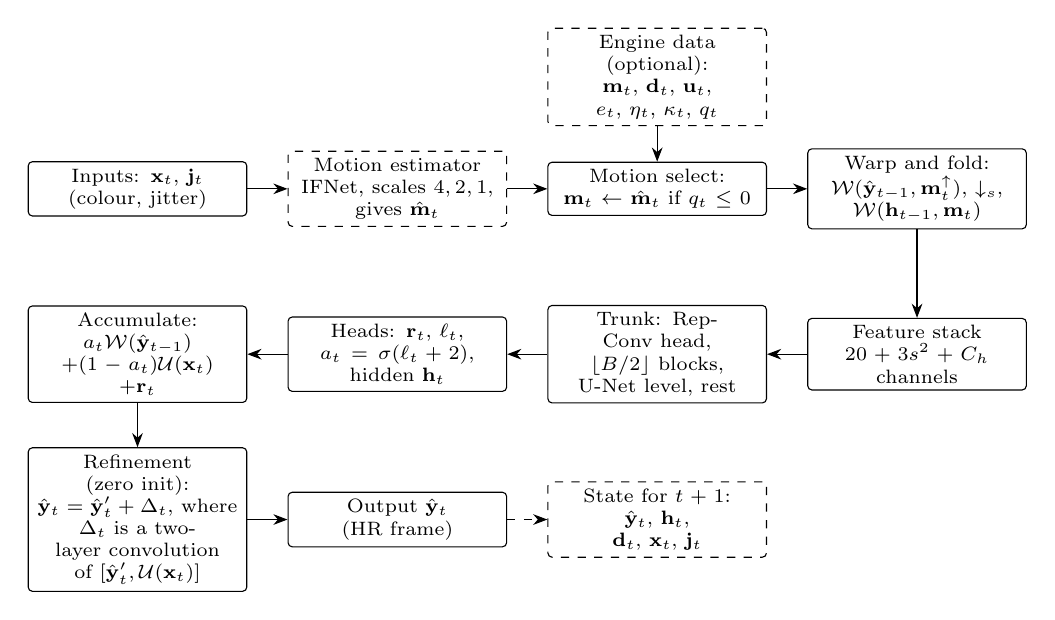
\begin{tikzpicture}[font=\scriptsize, node distance=0pt,
  box/.style={draw, rounded corners=1.5pt, align=center, text width=2.6cm, inner sep=2.5pt},
  opt/.style={box, dashed},
  arr/.style={-{Stealth[length=1.8mm]}},
  rec/.style={-{Stealth[length=1.8mm]}, dashed}]
\node[box] (in) at (0,6.0) {Inputs: $\mathbf{x}_t$, $\mathbf{j}_t$\\(colour, jitter)};
\node[opt] (est) at (3.3,6.0) {Motion estimator\\IFNet, scales $4,2,1$,\\gives $\hat{\mathbf{m}}_t$};
\node[box] (sel) at (6.6,6.0) {Motion select:\\$\mathbf{m}_t\leftarrow\hat{\mathbf{m}}_t$ if $q_t\le 0$};
\node[box] (warp) at (9.9,6.0) {Warp and fold:\\$\mathcal{W}(\hat{\mathbf{y}}_{t-1},\mathbf{m}_t^{\uparrow})$, $\downarrow_s$,\\$\mathcal{W}(\mathbf{h}_{t-1},\mathbf{m}_t)$};
\node[opt, above=0.45cm of sel] (eng) {Engine data (optional):\\$\mathbf{m}_t$, $\mathbf{d}_t$, $\mathbf{u}_t$,\\$e_t$, $\eta_t$, $\kappa_t$, $q_t$};
\node[box] (stack) at (9.9,3.9) {Feature stack\\$20+3s^2+C_h$ channels};
\node[box] (trunk) at (6.6,3.9) {Trunk: RepConv head,\\$\lfloor B/2\rfloor$ blocks,\\U-Net level, rest};
\node[box] (heads) at (3.3,3.9) {Heads: $\mathbf{r}_t$, $\ell_t$,\\$a_t=\sigma(\ell_t+2)$,\\hidden $\mathbf{h}_t$};
\node[box] (acc) at (0,3.9) {Accumulate:\\$a_t\mathcal{W}(\hat{\mathbf{y}}_{t-1})$\\$+(1-a_t)\mathcal{U}(\mathbf{x}_t)$\\$+\mathbf{r}_t$};
\node[box] (refine) at (0,1.8) {Refinement (zero init):\\$\hat{\mathbf{y}}_t=\hat{\mathbf{y}}'_t+\Delta_t$, where\\$\Delta_t$ is a two-layer convolution\\of $[\hat{\mathbf{y}}'_t,\mathcal{U}(\mathbf{x}_t)]$};
\node[box] (out) at (3.3,1.8) {Output $\hat{\mathbf{y}}_t$\\(HR frame)};
\node[opt] (state) at (6.6,1.8) {State for $t+1$:\\$\hat{\mathbf{y}}_t$, $\mathbf{h}_t$,\\$\mathbf{d}_t$, $\mathbf{x}_t$, $\mathbf{j}_t$};
\draw[arr] (in) -- (est);
\draw[arr] (est) -- (sel);
\draw[arr] (sel) -- (warp);
\draw[arr] (eng) -- (sel);
\draw[arr] (warp) -- (stack);
\draw[arr] (stack) -- (trunk);
\draw[arr] (trunk) -- (heads);
\draw[arr] (heads) -- (acc);
\draw[arr] (acc) -- (refine);
\draw[arr] (refine) -- (out);
\draw[rec] (out) -- (state);
\end{tikzpicture}
\caption{Data flow of one TSR time step at scale $s$. Dashed boxes are optional: the engine data are used when the caller supplies them, and the estimator runs in training for every frame and at inference only when a sample has no motion. The state of frame $t$ holds the history, hidden state, depth, colour and jitter that the warp and disocclusion cue of frame $t+1$ read (\cref{sec:tsrm-state})}\label{fig:tsrm-arch}
\end{figure}

\FloatBarrier

\subsection{Inputs}\label{sec:tsrm-inputs}

The trunk receives a stack of channels at render resolution. \Cref{tab:tsrm-inputs} lists them in the order of the code. Seventeen channels come from the frame and its side information, $3s^2$ from the folded history, three from the history disagreement and $C_h$ from the hidden state, so the stack has $20+3s^2+C_h$ channels. For $s=3$ and $C_h=8$ this is $55$, which the code confirms for the \tier{low} tier. The table gives the value that the network sees in each mode. Two replacements happen before the stack is built. A sample without motion receives the estimate $\hat{\mathbf{m}}_t$ and the flag $0.25$ (\cref{sec:tsrm-motion}). A sample with withheld depth receives zero depth and $\eta_t=0$.

The engine motion of the table is the motion in the input, which is exact (synthetic, TartanAir and Sintel), RAFT (real video and GameIR), or absent. The value $\tfrac12$ marks RAFT motion and video samples that keep their motion labels, which are capped at $\tfrac12$ by the degradation of \cref{sec:tsrm-data}.

The depth normalisation of \cref{tab:tsrm-inputs} is
\begin{equation}\label{eq:tsrm-depth}
\mathbf{d}_t=\frac{1}{1+\mathbf{d}^{\mathrm{raw}}_t/\operatorname{med}(\mathbf{d}^{\mathrm{raw}})},
\end{equation}
where $\mathbf{d}^{\mathrm{raw}}$ is the depth in the unit of its source, and $\operatorname{med}$ is the median over the whole sequence for synthetic samples, and over one frame for real windows and test clips. Non-positive and non-finite depth values are set to infinity before the normalisation, so they map to values near zero.

The normals are derived from the normalised depth with edge replication at the border, using the central differences $g^x_t(X,Y)=8\,[\mathbf{d}_t(X+1,Y)-\mathbf{d}_t(X-1,Y)]$ and $g^y_t$ defined in the same way along $Y$:
\begin{equation}\label{eq:tsrm-normal}
\mathbf{n}_t=\eta_t\,\frac{(-g^x_t,\,-g^y_t,\,1)}{\sqrt{(g^x_t)^2+(g^y_t)^2+1}}.
\end{equation}
The factor $8$ is a fixed constant of the code that scales the depth gradient, and the vector is normalised to unit length.

The disocclusion cue compares the current depth with the depth of the previous frame warped to the current frame, using the motion of the network:
\begin{equation}\label{eq:tsrm-disocc}
\delta_t=\eta_t\,\min\Big\{1,\ \frac{\lvert\mathbf{d}_t-\mathcal{W}(\mathbf{d}_{t-1},\mathbf{m}_t)\rvert}{\lvert\mathbf{d}_t\rvert+10^{-3}}\Big\}.
\end{equation}
A large value marks a depth that differs from the warped previous depth, which is typical of a disocclusion. It is a heuristic that the trunk refines, not a visibility test.

\subsection{Motion estimator}\label{sec:tsrm-motion}

The estimator is the IFNet of RIFE 4.26 \cite{huang2022rife} in a narrower form, a coarse-to-fine chain of flow blocks. It is built by \texttt{IFNet(widths, n\_res, n\_hint=3)} in \texttt{nss\_models.py}. Its widths and residual counts are set per tier in the constant \texttt{TSR\_TIERS}: $(32,24,16)$ with two residual blocks for \tier{igpu}, $(48,32,24)$ with three for \tier{low}, $(64,48,32)$ with four for \tier{mid}, $(96,64,48)$ with four for \tier{high}, and $(128,96,64)$ with six for \tier{teacher}. The three levels run at scales $\sigma_1=4$, $\sigma_2=2$ and $\sigma_3=1$ relative to the LR frame, so the coarsest block sees a frame of a quarter of the LR size in each direction.

The estimator takes the previous colour frame $\mathbf{x}_{t-1}$ and the current frame $\mathbf{x}_t$, both padded at the right and bottom by edge replication to multiples of $16$. Its timestep is the constant $1$, so its target frame is the current frame and its reference is the previous one. Its final flow, the first two of its four channels, is the motion of \cref{sec:tsrm-problem}:
\begin{equation}\label{eq:tsrm-est}
\hat{\mathbf{m}}_t=\mathbf{F}^{(3)}_{0},\qquad \mathbf{F}^{(1)}=\Delta^{(1)},\qquad \mathbf{F}^{(k)}=\mathbf{F}^{(k-1)}+\Delta^{(k)}\ \ (k=2,3),
\end{equation}
where $\Delta^{(k)}$ is the four-channel flow update of block $k$ and $\mathbf{F}^{(k)}=(\mathbf{F}^{(k)}_0,\mathbf{F}^{(k)}_1)$ holds the flows from the target to the previous and to the current frame. The flow outputs are multiplied by the block scale, so the flows stay in LR pixels.

The first block receives $\mathbf{x}_{t-1}$, $\mathbf{x}_t$, the per-frame features of both frames and the constant timestep, which is $15$ channels. Each later block receives the colour of both frames warped by the current flow, the features of both frames warped by the current flow, the timestep, the blend mask and the features of the previous block, and the current flow itself, which is $28$ channels. Three hint channels follow for the TSR estimator: the jitter difference $\mathbf{j}_t-\mathbf{j}_{t-1}$ (two channels) and the input kind $\kappa_t$ (one channel). The per-frame feature encoder has a stride-two $3\times3$ convolution and two $3\times3$ convolutions, each followed by LeakyReLU, and a transposed convolution that returns to full resolution with four channels. Inside each block, two stride-two $3\times3$ convolutions reduce the resolution by four, a set of residual $3\times3$ convolutions with a learned per-channel scale follows, and a transposed convolution with pixel shuffle returns to the block resolution with $4$ flow channels, one mask logit and $8$ features.

The estimator is initialised from the RIFE 4.26 weights wherever the names match, and its narrower layers take the leading channel slices of the RIFE tensors. The weight loader \texttt{load\_ifnet\_weights} copies the matching tensors whole and the narrower ones as slices, and the hint channels keep their zero weights. The training log of the \tier{low} run records the result as 11 whole tensors and 42 sliced tensors with no missing tensor. Without the RIFE weights, the code falls back to random initialisation and logs the fact.

The estimate replaces the motion only where the caller gave none. The rule is the one line of \texttt{TSRNet.forward}:
\begin{equation}\label{eq:tsrm-select}
\mathbf{m}_t=\begin{cases}\bar{\mathbf{m}}_t\ \text{(teacher-forced label)} & \text{if } q_t\le 0 \text{ and the sample is forced},\\ \hat{\mathbf{m}}_t & \text{if } q_t\le 0 \text{ otherwise},\\ \text{given motion} & \text{if } q_t>0,\end{cases}
\end{equation}
and the quality flag of every sample with $q_t\le 0$ becomes $\tfrac14$ (the constant \texttt{EST\_MV\_QUALITY}). The flag is therefore the same for estimated and forced samples, and the network cannot tell them apart. At inference the estimator runs only when some sample of the batch has $q_t\le 0$. In training it runs for every frame of every sample, because the motion loss of \cref{sec:tsrm-loss} supervises every sample that has a label, including those with engine motion.

Teacher forcing protects the trunk while the estimator is still poor. A sample without motion is forced to warp its history with the label motion $\bar{\mathbf{m}}_t$ with probability $\pi(\tau)$, drawn once per sample and used for all its frames, where $\tau$ is the elapsed training time and $T_b$ the training budget in seconds:
\begin{equation}\label{eq:tsrm-teacher}
\pi(\tau)=\max\Big(0,\ 1-\frac{\tau}{\rho\,T_b}\Big),\qquad \rho=\Res{tsr.config.cfg.mv_warmup_frac}.
\end{equation}
The forcing applies only to samples that have a label, so $\lambda>0$. Its probability falls linearly from one to zero over the first quarter of the budget, after which no forced mask is drawn. The clock is the wall-clock time of each process from its first step, so the two DDP ranks draw their masks on their own clocks. Teacher forcing is the name for feeding a recurrent predictor a target in place of its own output during training. Here it is this code's schedule, which replaces the estimate by the label for part of the early training only.

\subsection{Warping, folding and the recurrent state}\label{sec:tsrm-state}

The state carried from frame $t-1$ to frame $t$ is
\begin{equation}\label{eq:tsrm-state}
\mathcal{S}_{t-1}=\big(\hat{\mathbf{y}}_{t-1},\ \mathbf{h}_{t-1},\ \mathbf{d}_{t-1},\ \mathbf{x}_{t-1},\ \mathbf{j}_{t-1}\big).
\end{equation}
The depth, colour and jitter are kept for the disocclusion cue and for the estimator of frame $t$. The ONNX export passes them as explicit inputs (\cref{sec:tsrm-deploy}).

The previous output is warped to the HR grid with the upsampled motion. The LR motion is interpolated bilinearly to HR and multiplied by the scale, because a displacement of $d$ LR pixels is $sd$ HR pixels:
\begin{equation}\label{eq:tsrm-up-motion}
\mathbf{m}_t^{\uparrow}=s\cdot\mathrm{Bil}^{\times s}[\mathbf{m}_t],\qquad \mathbf{H}_t=\mathcal{W}\big(\hat{\mathbf{y}}_{t-1},\mathbf{m}_t^{\uparrow}\big),
\end{equation}
where $\mathrm{Bil}^{\times s}$ is bilinear upsampling by $s$ with align-corners set to false. The folded history is $\downarrow_s\mathbf{H}_t\in\mathbb{R}^{3s^2\times h\times w}$, the space-to-depth rearrangement of PyTorch's pixel unshuffle, which places every $s\times s$ block of HR pixels in the channels of one LR pixel. The history disagreement uses the mean of each block, $\bar{\mathbf{H}}_t=\operatorname{avgpool}_s(\mathbf{H}_t)$, and its absolute difference to the LR colour, $\mathbf{g}_t=\lvert\bar{\mathbf{H}}_t-\mathbf{x}_t\rvert$.

The hidden state and the depth are warped at LR with the LR motion $\mathbf{m}_t$, which is the motion of the network. The hidden state after frame $t$ is produced by the trunk, as \cref{sec:tsrm-output} gives. Warping uses the backward warp of \cref{eq:tsrm-warp}:
\begin{equation}\label{eq:tsrm-warp}
\mathcal{W}(I,\mathbf{m})(\mathbf{p})=I\big(\mathbf{p}+\mathbf{m}(\mathbf{p})\big),
\end{equation}
where $I$ is read bilinearly and clamped to its border. The implementation uses grid sampling with align-corners set to true, the convention of RIFE, so that the pixel centres of the first and last rows and columns lie on the image border.

On the first frame of a sequence, or in every frame of the no-history ablation, the state is empty. The history $\mathbf{H}_t$, the folded history, the history disagreement and the warped hidden state are all multiplied by zero, the disocclusion cue is computed against the current depth so that it is zero, and the history weight is set to zero exactly, not learned, by the rule
\begin{equation}\label{eq:tsrm-reset}
a_t=0\quad\text{when the state is empty.}
\end{equation}
The network has no other reset. It has no scene-cut detector, so the history weight must reject a cut by itself. The synthetic renderer produces no cuts, and the cache builders contain no cut filter, so a real window may contain a cut, and the training does not measure how often that happens.

\subsection{Reconstruction trunk}\label{sec:tsrm-trunk}

The trunk is a chain of re-parameterisable blocks, called RepConv here, in the sense of RepVGG \cite{ding2021repvgg} and ECBSR \cite{zhang2021ecbsr}. A RepConv block is trained as a sum of linear branches and deployed as one $3\times3$ convolution. A training forward pass folds the branches into one kernel on every call, so each block costs one convolution in training and one in deployment. The folded kernel for an output channel $o$ and an input channel $i$ is
\begin{equation}\label{eq:tsrm-fold}
\mathbf{W}_{oi}=\mathbf{W}^{(3)}_{oi}+\operatorname{pad}_{3\times3}\big(\mathbf{W}^{(1)}_{oi}\big)+\sum_{k=1}^{3}\mathbf{P}_{o,i,k}\,\mathbf{E}_k+\delta_{oi}\,\mathbf{C},
\end{equation}
with the bias $b_o=b^{(3)}_o+b^{(1)}_o+b^{(e)}_o$. The symbols are as follows. $\mathbf{W}^{(3)}$ is a learned $3\times3$ kernel and $\mathbf{W}^{(1)}$ a learned $1\times1$ kernel, padded with zeros to $3\times3$. The matrices $\mathbf{E}_1$, $\mathbf{E}_2$ and $\mathbf{E}_3$ are the fixed Sobel-x, Sobel-y and Laplacian kernels, $[[-1,0,1],[-2,0,2],[-1,0,1]]$, $[[-1,-2,-1],[0,0,0],[1,2,1]]$ and $[[0,1,0],[1,-4,1],[0,1,0]]$. The coefficients $\mathbf{P}_{o,i,k}$ form a learned $1\times1$ convolution from $3C_i$ inputs to $C_o$ outputs, reshaped so that each input channel $i$ has its three edge responses $k$. The matrix $\mathbf{C}$ has a one at its centre and zeros elsewhere, and the term with $\delta_{oi}$ is present only when $C_i=C_o$. Because the folding is linear, the folded convolution computes exactly the same function as the training branches.

Each RepConv is followed by a PReLU with one learned slope per output channel, initialised to PyTorch's default of $0.25$. The side branches start at zero, in the following sense. The weights of the $1\times1$ branch and of the edge branch are set to zero, so the block starts as a $3\times3$ convolution plus identity. Their biases keep PyTorch's default uniform initialisation, so the side branches do not start exactly at zero. The code records that default initialisation grew the activations by about $1.9$ times per block and gave a non-finite teacher loss from step $10$ in an earlier run \Observation.

The trunk of \cref{eq:tsrm-trunk-def} is built from the stack $\mathbf{z}_t$, which has $20+3s^2+C_h$ channels. Let $\mathrm{RC}_{\mathrm{head}}$ denote the head RepConv block, $\mathcal{A}$ the first $\lfloor B/2\rfloor$ blocks, $\mathcal{B}$ the remaining $B-\lfloor B/2\rfloor$ blocks, and $\mathcal{V}$ the U-Net level, which exists when $U>0$:
\begin{align}
\mathbf{z}_0&=\mathrm{RC}_{\mathrm{head}}(\mathbf{z}_t) \label{eq:tsrm-trunk-def}\\
\mathbf{z}_1&=\mathcal{A}(\mathbf{z}_0)\nonumber\\
\mathbf{z}_2&=\mathbf{z}_1+\mathcal{V}(\mathbf{z}_1)\nonumber\\
\mathbf{y}_t&=\mathcal{B}(\mathbf{z}_2).\nonumber
\end{align}
The head is one RepConv from $20+3s^2+C_h$ channels to $C$ channels. The U-Net level, when present, is a $3\times3$ convolution with stride two from $C$ to $2C$ channels followed by PReLU, then $U$ RepConv blocks at $2C$ channels, then a $1\times1$ convolution from $2C$ to $4C$ channels and a pixel shuffle with factor two, which returns $C$ channels at LR resolution. The U-Net level therefore works at half the LR resolution and is added to the trunk as a residual. The LR input is padded to an even size by edge replication before the trunk, which the stride-two convolution needs. The numbers of blocks per tier are in \cref{tab:tsrm-tiers}.

\subsection{Output head and accumulation}\label{sec:tsrm-output}

The output head is one $3\times3$ convolution from $C$ to $4s^2$ channels, with zero weights and zero bias, applied to $\mathbf{y}_t$. A pixel shuffle with factor $s$ \cite{shi2016espcn} then gives four channels at HR. The first three are the residual $\mathbf{r}_t$ and the fourth is a logit $\ell_t$, and the history weight is
\begin{equation}\label{eq:tsrm-alpha}
a_t=\sigma(\ell_t+2),\qquad \sigma(z)=\frac{1}{1+e^{-z}}.
\end{equation}
At initialisation the zero weights give $\ell_t=0$, so $a_t=\sigma(2)\approx0.881$ and $\mathbf{r}_t=0$, and the network starts as a blend of the warped history and the upsampled colour. The hidden state is produced by a $3\times3$ convolution from $C$ to $C_h$ channels followed by $\tanh$, $\mathbf{h}_t=\tanh(\mathrm{Conv}_{3\times3}(\mathbf{y}_t))$, and it is warped at the next frame by \cref{eq:tsrm-warp}.

The output is the accumulation rule
\begin{equation}\label{eq:tsrm-acc}
\hat{\mathbf{y}}'_t=a_t\odot\mathcal{W}\big(\hat{\mathbf{y}}_{t-1},\mathbf{m}_t^{\uparrow}\big)+(1-a_t)\odot\mathcal{U}(\mathbf{x}_t)+\mathbf{r}_t,
\end{equation}
where $\odot$ is the element-wise product, $\mathcal{U}$ is the jitter-aware bilinear upsampling
\begin{equation}\label{eq:tsrm-up}
\mathcal{U}(\mathbf{x}_t)(X,Y)=\operatorname{Bil}[\mathbf{x}_t]\Big(\frac{X+\tfrac12}{s}-\mathbf{j}_t\Big),
\end{equation}
and $\operatorname{Bil}[\mathbf{x}]$ is the bilinear interpolant of the LR samples, sample $i$ at coordinate $i+\tfrac12$, with clamped borders. The term $\frac{X+1/2}{s}$ is the continuous LR coordinate of output pixel $(X,Y)$, and subtracting $\mathbf{j}_t$ reads each LR sample at its jittered position. The output is then refined as \cref{sec:tsrm-refine} gives. On the first frame, $a_t=0$ by \cref{eq:tsrm-reset}, so $\hat{\mathbf{y}}_0=\mathcal{U}(\mathbf{x}_0)+\mathbf{r}_0$.

\paragraph{Why this is a learned temporal accumulation.} Ignore the residual and the motion for a moment, and let $a_t=a$ be constant, with $\mathbf{m}_t=0$ on a static scene. Then \cref{eq:tsrm-acc} unrolls to
\begin{equation}\label{eq:tsrm-unroll}
\hat{\mathbf{y}}_t=a^{t}\,\mathcal{U}(\mathbf{x}_0)+\sum_{k=1}^{t}(1-a)\,a^{t-k}\,\mathcal{U}(\mathbf{x}_k).
\end{equation}
The weights add to one, because $a^t+(1-a)\sum_{j=0}^{t-1}a^j=a^t+(1-a^t)=1$. The sample $k$ frames old has weight $(1-a)a^{k}$, which is an exponential moving average over the frames of the sequence, with mean age $a/(1-a)$ frames. Each $\mathcal{U}(\mathbf{x}_k)$ reads the colour at a different sub-pixel jitter, so the average gathers the samples of several sub-pixel positions. This is the principle of temporal accumulation for supersampling \cite{yang2020taasurvey} (\cref{sec:bg-taa}). At the initial history weight $\sigma(2)$ the mean age is about $7.4$ frames.

Classical TAA has the same update with a fixed or heuristic blend weight, and it rectifies the reprojected history by clamping it to the colour neighbourhood of the current frame. \Cref{eq:tsrm-acc} keeps the update and changes the rectification. The weight $a_t$ is a learned per-pixel gate, and the network has the disagreement $\mathbf{g}_t$ as input and a receptive field of several convolutions, so the gate can learn to go to zero where the history is invalid, which happens at disocclusions and at particle effects. The residual $\mathbf{r}_t$ corrects the result additively. There is no explicit clamp anywhere in the TSR network, so the residual can move a pixel outside the neighbourhood of the current frame. The analytic baseline of \cref{sec:tsrm-test} does clamp, and the two rectifications are different.

\subsection{Refinement and the reset rule}\label{sec:tsrm-refine}

Every tier except \tier{igpu} refines the accumulated output at HR resolution. The refinement is
\begin{equation}\label{eq:tsrm-refine}
\hat{\mathbf{y}}_t=\hat{\mathbf{y}}'_t+\mathrm{Conv}_{3\times3}\Big(\mathrm{PReLU}\big(\mathrm{Conv}_{3\times3}([\hat{\mathbf{y}}'_t,\mathcal{U}(\mathbf{x}_t)])\big)\Big),
\end{equation}
where $[\cdot,\cdot]$ concatenates six channels. The first convolution has $R$ output channels and the second has three. The second convolution has zero weights and zero bias, so the refinement starts at the identity. Its purpose is to remove the pixel-shuffle pattern of the LR head, as the code comment states. The width $R$ is $8$ for \tier{low} and \tier{mid}, $12$ for \tier{high} and $16$ for the teacher, and the \tier{igpu} tier has no refinement.

The reset rule is \cref{eq:tsrm-reset}. It applies to the first frame of each training window and each test clip, and in every frame of the no-history ablation (\cref{sec:tsrm-abl}). The ONNX step of \cref{sec:tsrm-deploy} has no reset input.

\subsection{Model tiers}\label{sec:tsrm-tiers}

The tiers are the entries of \texttt{TSR\_TIERS} in \texttt{nss\_models.py}. \Cref{tab:tsrm-tiers} gives their widths, block counts, U-Net blocks, hidden widths, estimator, refinement width, parameter counts and costs. The parameter counts are those of the fused network, with the estimator included, and the estimator parameters are the difference from the same network built without the estimator. The costs count multiply-accumulates of every convolution, including the estimator, for one steady-state frame with history, per 1080p output frame, and exclude the warps and the pixel shuffles, which have no multiply-accumulates. The counting is done with forward hooks on the fused network in \texttt{tsr\_macs\_per\_lr\_pixel}, and the notebook scales it by the LR pixel count.

The fused parameter counts and the 3x and 2x costs are the values that \texttt{model\_tiers.csv} records for the run. They were also recomputed from \texttt{src/neuralss/nss\_models.py} on the current code, and both agree. The estimator column is the difference between the training parameter count with and without the estimator, which is also computed from the code. The \tier{mid} and \tier{high} tiers are defined and costed, but the TSR notebook never trains them. Its runs use the teacher at 3x, \tier{low} at 3x and 2x, \tier{igpu} at 3x, and the six ablation runs at 3x, which all use \tier{low}. The tier table of the article (\cref{M-tab:tiers}) therefore gives no latency for these two tiers.

The estimator holds a large share of the training parameters of every tier. It is about $81$ percent for \tier{igpu}, $63$ percent for \tier{low} and $51$ percent for the teacher, and it runs on every frame without engine motion.

\subsection{Training samples and degradations}\label{sec:tsrm-data}

Each training step draws from two streams, and both produce sequences of $T$ frames with HR targets, LR inputs, motion labels and validity masks. The synthetic stream renders layered game-like scenes from cached texture crops with the renderer of \cref{sec:data-synth}. Its scene parameters, which are used here, are a background layer and a foreground layer with procedural alpha (a superellipse, four thin wires each present with probability $0.6$, and a fence present with probability $0.35$), moving on continuous affine paths. The foreground texture is flat with probability $0.25$ and is otherwise the still of the neighbouring sample in the batch, the foreground layer is present with probability $0.85$, world-space text tiles are stamped into the background with probability $0.3$, and six particles are drawn, each active with probability $0.5$. The motion class is static, slow, medium or fast with probabilities $0.15$, $0.45$, $0.25$ and $0.15$, which give speeds of $0$, $0.3$ to $3$, $3$ to $10$ and $10$ to $28$ output pixels per frame. Each sample has an exposure $2^{u}$ with $u$ uniform on $[-0.8,0.8]$, and a sub-pixel jitter phase drawn uniformly from the sixteen Halton offsets. The LR frames are single-sample jittered reads of the renderer, and the HR targets are four-sample renders.

The real stream reads cached windows of $T$ frames at $P=192$ output pixels from the sequence sources of \cref{sec:data}. The window is drawn from a source-specific downscale range before cropping. A real window is flipped horizontally with probability $\tfrac12$ and vertically with probability $\tfrac12$, and its motion vectors are negated in the flipped components. It is scaled in linear light by an exposure gain $2^{u}$ with $u$ uniform on $[-0.8,0.8]$. Its LR frames are jittered bilinear reads of the HR frame, so they are aliased like a render. The labels are the cached motion and validity, with the label quality of the window. Exact motion, from TartanAir and Sintel, has label quality $1$. Other windows get RAFT motion when RAFT is available, with label quality $\tfrac12$, and otherwise zero motion with label quality $0$. \Cref{tab:tsrm-mix} lists the probabilities that the TSR configuration or the degradation functions set.

\begin{table}[!htbp]
\caption{Probabilities of the TSR training data that are set by the TSR configuration or by the degradation functions. The renderer's own probabilities are given in \cref{sec:tsrm-data} and \cref{sec:data-synth}}\label{tab:tsrm-mix}
{\scriptsize\raggedright\setlength{\tabcolsep}{3pt}
\begin{tabular*}{\textwidth}{@{\extracolsep\fill}p{0.44\textwidth}p{0.16\textwidth}p{0.32\textwidth}}
\toprule
Quantity & Value & Code location \\
\midrule
Real windows per batch & $\Res{tsr.config.cfg.p_real}$, so $19$ of $48$ & \texttt{p\_real}, \texttt{make\_loader} \\
Synthetic samples turned into plain video & $\Res{tsr.config.cfg.p_video_synth}$ & \texttt{p\_video\_synth}, \texttt{video\_degrade} \\
Real samples turned into plain video & $\Res{tsr.config.cfg.p_video_real}$ & \texttt{p\_video\_real}, \texttt{video\_degrade} \\
Plain-video samples that keep their motion labels & $\Res{tsr.config.cfg.p_video_mv}$ & \texttt{p\_video\_mv}, \texttt{video\_degrade} \\
Samples that lose their motion vectors (all samples of the batch) & $\Res{tsr.config.cfg.p_drop_mv}$ & \texttt{p\_drop\_mv}, \texttt{withhold\_engine\_data} \\
Samples that lose their depth (all samples of the batch) & $\Res{tsr.config.cfg.p_drop_depth}$ & \texttt{p\_drop\_depth}, \texttt{withhold\_engine\_data} \\
Long steps, every fourth step from step $0$ & $1/\Res{tsr.config.cfg.long_every}$ & \texttt{long\_every} $=\Res{tsr.config.cfg.long_every}$, \texttt{train\_tsr.step\_fn} \\
Teacher forcing of motion & $\pi(\tau)$ in \cref{eq:tsrm-teacher} & \texttt{mv\_warmup\_frac} $=\Res{tsr.config.cfg.mv_warmup_frac}$ \\
Horizontal and vertical flip of real windows & $1/2$ each & \texttt{sr\_batch\_from\_frames} \\
Gain of real windows and scene exposure & $2^{u}$, $u\sim U[-0.8,0.8]$ & \texttt{sr\_batch\_from\_frames}, \texttt{Scene} \\
Downscale filter of plain video (bicubic, bilinear, box) & $1/3$ each & \texttt{video\_lr} \\
Blur $\sigma$ of plain video & $U[0,0.6]$ output pixels & \texttt{video\_lr} \\
Noise $\sigma$ of plain video & $U[0,2/255]$ & \texttt{video\_lr} \\
\botrule
\end{tabular*}}
\end{table}

The plain-video degradation turns a sample into ordinary video. A plain-video LR frame is the target frame $\mathbf{y}$ after a Gaussian blur, an anti-aliased downscale, additive noise and 8-bit quantisation. The blur is a five-tap separable Gaussian on the output grid with $\sigma$ uniform on $[0,0.6]$. The downscale $D$ is bicubic (cubic convolution \cite{keys1981bicubic}), bilinear or box averaging, each chosen with probability $1/3$. The noise is added after the downscale, with $\sigma_n$ uniform on $[0,2/255]$, and the frame is clamped and rounded to multiples of $1/255$:
\begin{equation}\label{eq:tsrm-video}
\mathbf{x}^{\mathrm{vid}}_t=\mathrm{round}_{1/255}\Big(\mathrm{clip}_{[0,1]}\big(D\big(G_\sigma\ast\mathbf{y}_t\big)+\mathbf{n}\big)\Big),\qquad \mathbf{n}\sim\mathcal{N}(0,\sigma_n^2 I).
\end{equation}
A plain-video sample loses its jitter, its depth, its reactive mask and its depth availability, and its input kind becomes $\kappa_t=0$. Its motion is removed, except for the share $p_\mathrm{mv}=0.15$ that keeps the label motion with flag $\min(q,\tfrac12)$. The label motion of a plain-video sample is the block mean of the HR motion, divided by $s$, and its validity is one only where all $s\times s$ HR pixels are valid. The labels keep their label quality, so a plain-video sample still supervises the estimator.

The withholding rule is applied to the whole batch after both streams are built. Its two masks are drawn once per sample and apply to every sample, including the plain-video samples that kept their motion. A sample loses its motion with probability $0.25$, and it loses its depth with probability $0.3$. A plain-video sample that kept its motion therefore loses it with probability $0.25$.

Most real windows come from Vimeo-90K \cite{xue2019vimeo}, and only a small share has exact motion, as \cref{M-sec:discussion} reports \UnderRevision. The configuration gives the cache capacities of \Res{tsr.config.cfg.cache.still_train} still crops and \Res{tsr.config.cfg.cache.win_train} windows.

\subsection{Unroll lengths and patch sizes}\label{sec:tsrm-unroll}

Each training window has $T=\Res{tsr.config.cfg.seq_len}$ frames of $P=\Res{tsr.config.cfg.patch}$ output pixels, which is $64$ LR pixels at $s=3$ and $96$ at $s=2$. The network runs through the frames of a window in order, the state starts empty, and the loss of every frame is summed before one backward pass. The gradient flows through every frame of the window, and it stops at the window boundary, which is truncated back-propagation through time \cite{williams1990efficient}. The notebook gives six frames per window, as truncated back-propagation through the recurrence, and 192-pixel patches as its defaults. It sets $\Res{tsr.config.cfg.still_size}$-pixel texture crops so that fast camera paths have room inside the texture.

Every fourth step is a long step with $T=\Res{tsr.config.cfg.long_t}$ frames of $P=\Res{tsr.config.cfg.long_patch}$ pixels, which is $16\times96^2=147{,}456$ output pixels per window, two thirds of the $6\times192^2=221{,}184$ of a normal window. The notebook gives the reason for the long steps as the decline of the earlier students on static scenes after frames $6$ to $10$, which the notebook measured in one earlier run \Preliminary. The long steps use only synthetic windows, so each GPU has $48-19=29$ of them in a long step, against $48$ windows in a normal step.

The batch is $48$ windows per GPU for the teacher and for the students. The batch probe of the notebook tried sizes $4$, $8$, $12$, $16$, $24$, $32$ and $48$, and it kept the largest size that stayed below $75$ percent of GPU memory. Both models passed at $48$ with memory use well below that limit, so the list, not the memory, set the batch. The main stages run on both GPUs with distributed data parallel, which gives $96$ windows per step, and the paired runs and ablations run on one GPU each, with $48$ windows per step.

\subsection{Loss}\label{sec:tsrm-loss}

The loss is computed for every window and then averaged over the batch. For the frames $t=0,\dots,T-1$ of a window, let $\hat{\mathbf{y}}_t$ be the output and $\mathbf{y}_t$ the target. The pixel term is a Charbonnier penalty, with $\varepsilon=10^{-3}$, averaged over the frames with weight $\tfrac14$ on the first frame, which has no history:
\begin{equation}\label{eq:tsrm-lpix}
\mathcal{L}_\mathrm{pix}=\frac{\sum_{t}\omega_t\,\mathbb{E}\sqrt{(\hat{\mathbf{y}}_t-\mathbf{y}_t)^2+\varepsilon^2}}{\sum_t\omega_t},\qquad \omega_0=\tfrac14,\ \ \omega_t=1\ \ (t\ge1).
\end{equation}
The expectation $\mathbb{E}$ is the mean over the channels and pixels of the batch. The Charbonnier penalty \cite{charbonnier1997deterministic} is a smooth edge-preserving potential that approximates the absolute difference.

The gradient term compares the finite differences of the output and the target over a distance of two pixels in each direction. With $D_x\mathbf{z}(X,Y)=\mathbf{z}(X+2,Y)-\mathbf{z}(X,Y)$ and $D_y$ defined in the same way along $Y$,
\begin{equation}\label{eq:tsrm-lgrad}
\mathcal{L}_\mathrm{grad}=\mathbb{E}_t\big|D_x\hat{\mathbf{y}}_t-D_x\mathbf{y}_t\big|+\mathbb{E}_t\big|D_y\hat{\mathbf{y}}_t-D_y\mathbf{y}_t\big|,
\end{equation}
where $\mathbb{E}_t$ is the mean over all frames of the window, the channels and the pixels.

The Fourier term compares the magnitudes of the two-dimensional spectra of the frames, computed with the orthonormal real FFT, so that texture energy at every frequency counts:
\begin{equation}\label{eq:tsrm-lfft}
\mathcal{L}_\mathrm{fft}=\mathbb{E}_t\Big|\,\big|\mathcal{F}\hat{\mathbf{y}}_t\big|-\big|\mathcal{F}\mathbf{y}_t\big|\,\Big|,
\end{equation}
where $\mathcal{F}$ is the orthonormal real two-dimensional FFT of each channel and $|\cdot|$ is the complex magnitude.

The temporal term matches the change of the output to the change of the target along the label motion, at HR, over the pixels that are visible in both frames:
\begin{multline}\label{eq:tsrm-ltmp}
\mathcal{L}_\mathrm{tmp}=\frac{1}{T-1}\sum_{t=1}^{T-1}\frac{\sum_{\mathbf{p}}\bar{\mathbf{V}}_t(\mathbf{p})\,\lambda_t\sum_{c}\big|\Delta^{\mathrm{out}}_{t,c}(\mathbf{p})-\Delta^{\mathrm{gt}}_{t,c}(\mathbf{p})\big|}{3\sum_{\mathbf{p}}\bar{\mathbf{V}}_t(\mathbf{p})\,\lambda_t+10^{-6}},
\end{multline}
where $\Delta^{\mathrm{out}}_t=\hat{\mathbf{y}}_t-\mathcal{W}(\hat{\mathbf{y}}_{t-1},\bar{\mathbf{M}}_t)$ and $\Delta^{\mathrm{gt}}_t=\mathbf{y}_t-\mathcal{W}(\mathbf{y}_{t-1},\bar{\mathbf{M}}_t)$ are the temporal changes of the output and of the target along the label motion, $\bar{\mathbf{M}}_t$ is the HR label motion, $\bar{\mathbf{V}}_t$ its validity and $\lambda_t$ its label quality. The term is zero for windows without labels.

The motion term supervises the estimator on every frame after the first, with the LR label motion $\bar{\mathbf{m}}_t$ and its validity $\bar{\mathbf{v}}_t$:
\begin{equation}\label{eq:tsrm-lflow}
\mathcal{L}_\mathrm{flow}=\frac{\sum_{t=1}^{T-1}\sum_{\mathbf{p}}\lambda_t\,\bar{\mathbf{v}}_t(\mathbf{p})\,\big\lVert\hat{\mathbf{m}}_t(\mathbf{p})-\bar{\mathbf{m}}_t(\mathbf{p})\big\rVert_1}{\sum_{t=1}^{T-1}\sum_{\mathbf{p}}\lambda_t\,\bar{\mathbf{v}}_t(\mathbf{p})+1},
\end{equation}
where $\lVert\cdot\rVert_1$ sums the absolute differences of the two components, so the error is measured in LR pixels. The $+1$ in the denominator avoids a division by zero when no window has a valid label.

The perceptual term is LPIPS \cite{zhang2018lpips} with its AlexNet backbone on the last frame of the window, computed on the output clamped to $[0,1]$:
\begin{equation}\label{eq:tsrm-llp}
\mathcal{L}_\mathrm{lp}=\mathbb{E}_{\mathrm{batch}}\,\mathrm{LPIPS}\big(\mathrm{clip}_{[0,1]}(\hat{\mathbf{y}}_{T-1}),\mathbf{y}_{T-1}\big).
\end{equation}
The distillation term $\mathcal{L}_\mathrm{kd}$ is the mean absolute difference between the output and the output of a frozen teacher on the same inputs. It is inactive (\cref{sec:tsrm-distill}). The total loss is
\begin{equation}\label{eq:tsrm-loss}
\mathcal{L}=\mathcal{L}_\mathrm{pix}+\Res{tsr.config.cfg.w_grad}\,\mathcal{L}_\mathrm{grad}+\Res{tsr.config.cfg.w_fft}\,\mathcal{L}_\mathrm{fft}+\Res{tsr.config.cfg.w_temporal}\,\mathcal{L}_\mathrm{tmp}+\Res{tsr.config.cfg.w_flow}\,\mathcal{L}_\mathrm{flow}+\Res{tsr.config.cfg.w_lpips}\,\mathcal{L}_\mathrm{lp}+\Res{tsr.config.cfg.w_distill}\cdot\mathcal{L}_\mathrm{kd}.
\end{equation}
The weights are the configuration values \texttt{w\_grad}, \texttt{w\_fft}, \texttt{w\_temporal}, \texttt{w\_flow}, \texttt{w\_lpips} and \texttt{w\_distill} of the run. The frames that each term uses are stated with its equation, and the validation metric is not part of the loss.

\subsection{Optimisation, schedule, precision, moving average and checkpoints}\label{sec:tsrm-optim}

The optimiser is AdamW \cite{loshchilov2019adamw} with betas $(0.9,\,0.99)$, PyTorch's default $\epsilon=10^{-8}$ and weight decay $\Res{tsr.config.cfg.weight_decay}$, applied to every parameter. The peak learning rate is $\Res{tsr.config.cfg.lr}$ for the students and $\Res{tsr.config.cfg.lr_teacher}$ for the teacher. The learning rate follows the wall-clock budget. Let $\varrho=\tau/T_b$ be the fraction of the budget used, with $\varrho_w=\Res{tsr.config.cfg.warmup_frac}$, $\alpha_0$ the peak learning rate and $\alpha_\mathrm{min}=\Res{tsr.config.cfg.min_lr}$:
\begin{equation}\label{eq:tsrm-lr}
\alpha(\varrho)=\begin{cases}\alpha_0\,\max\big(\varrho/\varrho_w,\ 0.01\big), & \varrho<\varrho_w,\\[2pt] \alpha_\mathrm{min}+\tfrac12(\alpha_0-\alpha_\mathrm{min})\Big(1+\cos\Big(\pi\,\dfrac{\varrho-\varrho_w}{1-\varrho_w}\Big)\Big), & \varrho\ge\varrho_w.\end{cases}
\end{equation}
The first $3$ percent of the budget is a linear warm-up from $0.01\,\alpha_0$, and the rest is a single cosine decay without restarts, the decay used within each cycle of SGDR \cite{loshchilov2017sgdr}. The rate is updated every $10$ steps, together with the decision to stop and the validation check, because the processes agree on the elapsed time only at those points.

The gradients are unscaled and their global $L_2$ norm is clipped to $1$ before the optimiser step. The forward pass of the network and of the teacher, when there is one, runs under FP16 autocast, and the losses are computed in FP32 \cite{micikevicius2018mixed}. A dynamic gradient scaler with PyTorch's default initial scale multiplies the loss before the backward pass, and it skips the step when a gradient is non-finite. A run whose loss stays non-finite for $200$ steps stops with an error, so that a diverged run does not use its whole budget.

The moving average of the weights is the recursion below, which is this work's choice.
\begin{equation}\label{eq:tsrm-ema}
\theta^{\mathrm{EMA}}_k=d_k\,\theta^{\mathrm{EMA}}_{k-1}+(1-d_k)\,\theta_k,\qquad d_k=\min\Big(\Res{tsr.config.cfg.ema_decay},\ \frac{1+k}{10+k}\Big),
\end{equation}
where $k\ge1$ counts the updates of the average on rank $0$. The warm-up rule $\min\big((1+k)/(10+k),\ \mathrm{decay}\big)$ is this code's choice, and it makes the averaging window $1/(1-d_k)=(10+k)/9$ updates at update $k$, until the cap $\Res{tsr.config.cfg.ema_decay}$ is reached at $k\approx8{,}990$ updates. The average is therefore short for most of a run and reaches its full window only late in the run, and the validation and the checkpoints of \cref{sec:tsrm-test} use the averaged weights.

Validation runs every $\min(\Res{tsr.config.cfg.val_interval_min}\text{ min},\ \max(T_b/6,\ 60\text{ s}))$ and once more at the end of the budget. It uses a fixed validation set: the first $32$ still crops and the first $32$ windows of the validation caches, in \Res{tsr.config.cfg.val_batches} batches of $\Res{tsr.config.cfg.val_bs}$ still crops and $\Res{tsr.config.cfg.val_bs}$ windows, each evaluated twice. The render copy keeps the engine data, and the plain-video copy degrades every sample with the probability $1$ of \cref{sec:tsrm-data}. The score is the PSNR on luma (\cref{eq:tsrm-psnr}) over the frames $1$ to $T-1$ of each window, with the $s$-pixel border removed, averaged over the windows of each copy, and the selection score is the mean of the two copies.

Each validation round saves the raw and the averaged weights. The averaged weights of the first round with the highest score are kept separately, and evaluation loads them.

The stage budgets are $\Res{tsr.config.cfg.minutes.teacher}$ minutes for the teacher, $\Res{tsr.config.cfg.minutes.student}$ minutes for the \tier{low} student at $3\times$, $\Res{tsr.config.cfg.minutes.pair}$ minutes for each of the paired \tier{igpu} at $3\times$ and \tier{low} at $2\times$ runs, and $\Res{tsr.config.cfg.minutes.ablation}$ minutes for each ablation. The seeds are the configuration seed $\Res{tsr.config.cfg.seed}$ plus the rank for the model, and $100\times\Res{tsr.config.cfg.seed}$ plus the rank for the generator of the synthetic renderer, which keeps every rank's random streams apart. The data loader draws its windows from memory-mapped caches without replacement inside a batch, and each batch index selects its own random generator seed.

\subsection{Per-frame training loop}\label{sec:tsrm-loop}

The training loop of \texttt{train\_loop} and \texttt{train\_tsr.step\_fn} runs the following steps for every iteration on each rank.

\begin{enumerate}
\item Draw one batch from the memory-mapped caches: $19$ real windows and $29$ synthetic still crops on each GPU in a normal step. The indices are sorted and drawn without replacement within the batch.
\item Decide the step type. A step whose index is a multiple of four is a long step, with $29$ synthetic windows of $16$ frames at $96$ pixels, and the teacher is not run. Otherwise the batch is $6$-frame windows, with the real windows in the batch.
\item Build the synthetic windows with the renderer (\texttt{sr\_batch}): motion class, jitter phase, exposure, particles, text, the LR jittered samples, the HR four-sample targets, the exact motion and validity at LR and HR, depth, and the reactive masks.
\item Build the real windows (\texttt{sr\_batch\_from\_frames}): random flips with the motion components negated, the exposure gain in linear light, jittered bilinear reads of the HR frames, and the cached motion, validity and depth.
\item Degrade the plain-video shares: a synthetic window with probability $0.3$, a real window with probability $0.6$, with the filter, blur and noise of \cref{eq:tsrm-video}. The degraded samples keep their motion labels with probability $0.15$.
\item Withhold the engine data of the batch: motion with probability $0.25$ and depth with probability $0.3$, drawn once per sample.
\item Compute the teacher-forcing probability $\pi(\tau)$ of \cref{eq:tsrm-teacher} from the elapsed time, draw the forced mask for the samples with no motion and a label, and add it to the batch when $\pi>0$.
\item Run the recurrent unroll under FP16 autocast. For each frame $t$ in order: form the inputs of \cref{tab:tsrm-inputs}, run the estimator for every frame in training, select the motion of \cref{eq:tsrm-select}, warp and fold the state, run the trunk and the heads, accumulate with \cref{eq:tsrm-acc}, refine with \cref{eq:tsrm-refine}, and keep the state for the next frame. The first frame starts from the reset state.
\item Compute the losses of \cref{eq:tsrm-lpix,eq:tsrm-lgrad,eq:tsrm-lfft,eq:tsrm-ltmp,eq:tsrm-lflow,eq:tsrm-llp} in FP32 and their weighted sum \cref{eq:tsrm-loss}.
\item Scale the loss, run the backward pass through the whole unroll, unscale the gradients, clip their global norm to $1$, and take one AdamW step. A non-finite gradient skips the step.
\item Update the moving average of the weights on rank $0$ with \cref{eq:tsrm-ema}.
\item Every $10$ steps, all-reduce the elapsed time, the stop flag and the memory counters. Set the learning rate by \cref{eq:tsrm-lr}, count the consecutive non-finite checks, and run the validation of \cref{sec:tsrm-optim} when the interval has passed or the budget has ended. Save the checkpoints and, when the validation score is a new best, the best averaged weights.
\item Stop when the budget is used, write the history of the rounds, and report the best round.
\end{enumerate}

\subsection{Distillation}\label{sec:tsrm-distill}

The training code contains a distillation path. A frozen teacher is unrolled on the same inputs without gradients, and its output enters the loss through \cref{eq:tsrm-loss} with weight $w_\mathrm{distill}$. No TSR run used it, because each run sets the teacher checkpoint to none and the weight to zero. The teacher of the article is therefore trained directly, as the quality ceiling, and not distilled. The earlier runs of 20 to 21 and 24 October 2026 recorded no measurable gain from distillation, which the notebook gives as the reason for switching it off \Preliminary.

\subsection{Ablation configurations}\label{sec:tsrm-abl}

Every ablation trains the \tier{low} tier at $3\times$ for $\Res{tsr.config.cfg.minutes.ablation}$ minutes, two at a time on the two GPUs, against a reference run of the same recipe and budget. \Cref{tab:tsrm-abl-config} lists what each one changes and how the change is implemented. The reference is the full recipe at the same budget.

\begin{table}[!htbp]
\caption{TSR ablation configurations. Each row changes one part of the \tier{low} recipe at $3\times$ and $\Res{tsr.config.cfg.minutes.ablation}$ minutes, against the reference}\label{tab:tsrm-abl-config}
{\scriptsize\raggedright\setlength{\tabcolsep}{3pt}
\begin{tabular*}{\textwidth}{@{\extracolsep\fill}p{0.31\textwidth}p{0.30\textwidth}p{0.31\textwidth}}
\toprule
Name & Change & Implementation \\
\midrule
\texttt{abl\_reference} & None & Full recipe with the same $30$-minute budget \\
\texttt{abl\_no\_history} & Single-frame upscaling: no history, no hidden state & \texttt{use\_history=False}: every frame resets (\cref{eq:tsrm-reset}), and unused parameters are allowed in DDP \\
\texttt{abl\_no\_gbuffers} & Colour-only render input: the estimator supplies the motion & \texttt{ablate\_gbuffers}: depth, motion, depth availability and motion quality are zero in every frame \\
\texttt{abl\_no\_motion\_net} & No motion estimator, colour-only input, zero motion & \texttt{motion\_net=False} and \texttt{ablate\_gbuffers}: no estimator and no motion loss \\
\texttt{abl\_no\_video\_training} & Render-like samples only & Both video shares set to zero, the \texttt{p\_video} keys of the configuration, and the withholding of \cref{sec:tsrm-data} still applies \\
\texttt{abl\_no\_long\_unroll} & Six-frame windows only & \texttt{long\_every}$=0$ \\
\botrule
\end{tabular*}}
\end{table}

Each ablation validates on batches built with its own recipe, so validation scores are not comparable between ablations. The test protocol of \cref{sec:tsrm-test} evaluates them all on the same suites. Its engine-mode evaluation of \texttt{abl\_no\_motion\_net} is an exception. The evaluation sets the colour-only flag only for \texttt{abl\_no\_gbuffers} and the no-history flag only for \texttt{abl\_no\_history}. The engine-mode rows of \texttt{abl\_no\_motion\_net} therefore receive depth and motion that the model was never trained with \UnderRevision. The plain-mode rows of this ablation are not affected, because plain inputs have no engine data, and \cref{M-tab:tsr-abl} uses only those rows.

\subsection{Fusion, precision and export}\label{sec:tsrm-deploy}

Fusion replaces every RepConv by a plain $3\times3$ convolution with the folded kernel and bias of \cref{eq:tsrm-fold}, followed by a copy of its PReLU. The rest of the network is unchanged. The motion estimator is built from ordinary convolutions and is not folded. The fused and unfused networks compute the same function up to floating-point error, and the notebook checks the difference on a synthetic batch of each scale and records the maximum absolute difference in FP32.

The evaluation and the latency measurements use the fused networks converted to FP16 weights, and the evaluation runs them under autocast. The latency is the mean over $100$ timed forward passes of one fused FP16 step at batch $1$, after $10$ warm-up steps, with CUDA events and cuDNN autotuning. It is measured at $1080$p and $2160$p outputs for $3\times$ and at $1080$p for $2\times$. The arithmetic estimate in the notebook is a parameter, not a measurement. All latencies are eager PyTorch on one T4, and in-engine latency on target GPUs is not measured \UnderRevision.

The ONNX export wraps one fused step with explicit state tensors. Its inputs are the colour, depth, motion, reactive mask, exposure, jitter, a flag vector of depth availability, motion quality and input kind, and the previous output, hidden state, depth, colour and jitter. Its outputs are the output and the new hidden state. The export uses opset $17$ with the TorchScript exporter, static shapes for one LR size (the notebook uses $36\times64$ and the scale), and it is checked with ONNX Runtime on the CPU against PyTorch in FP32. A deployment must export one graph per render resolution.

The exported step has no reset input. The caller supplies the previous output for the first frame, and the graph then blends that output with the learned weight $a_t$, instead of the zero weight of \cref{eq:tsrm-reset}. The notebook's export test runs a single frame and does not exercise the first frame of a sequence. An engine integration must therefore supply a valid previous output on the first frame, which the export does not check \UnderRevision.

\subsection{Test protocol}\label{sec:tsrm-test}

The test suites are built from the test split of the manifest, which the notebook loads before the evaluation and never uses for training. \Cref{tab:tsrm-suites} lists them. A clip is the first $T$ frames of an item, starting at frame $0$, cropped at the centre to the crop size of its suite. The first $4n$ items of a source with at least $T$ frames are tried, and a clip is skipped when it cannot be decoded or when one of its frames is blank, meaning a luma standard deviation below $2$ on the $0$ to $255$ scale. A blank frame would be reconstructed exactly by every method and would score the PSNR cap of $100$ dB. Clips with frozen frames or scene cuts are not filtered.

\begin{table}[!htbp]
\caption{TSR test suites. Motion labels are exact (renderer or exact flow) or RAFT. Each suite runs in both modes except GameIR, which runs in engine mode only}\label{tab:tsrm-suites}
{\scriptsize\raggedright\setlength{\tabcolsep}{3pt}
\begin{tabular*}{\textwidth}{@{\extracolsep\fill}p{0.19\textwidth}p{0.37\textwidth}p{0.17\textwidth}p{0.04\textwidth}p{0.12\textwidth}}
\toprule
Suite & Source and frame size & Motion & $T$ & Scales \\
\midrule
\texttt{synthetic-game} & Game stills and DIV2K \cite{agustsson2017div2k} test items, $1024$-pixel texture crops, rendered at $\Res{tsr.config.cfg.eval.synthetic_p}$ output pixels, six sequences per motion class & Exact & $\Res{tsr.config.cfg.eval.synthetic_t}$ & $3\times$, $2\times$ \\
\texttt{tartanair} & TartanAir \cite{wang2020tartanair} test environments, $480\times576$ & Exact (forward flow played backwards) & $\Res{tsr.config.cfg.eval.real_t}$ & $3\times$, $2\times$ \\
\texttt{sintel} & MPI Sintel \cite{butler2012sintel} test scene families, $432\times1008$ & Exact (with occlusion masks) & $\Res{tsr.config.cfg.eval.real_t}$ & $3\times$, $2\times$ \\
\texttt{vid4} & Vid4 \cite{liu2014vid4} test sequences, $480\times696$ & RAFT & $\Res{tsr.config.cfg.eval.real_t}$ & $3\times$, $2\times$ \\
\texttt{vimeo1080p} & Pinned validation shards of Vimeo-1080p, which the manifest assigns to the test split, shorter side at most $540$, crop $540\times960$ & RAFT & $\Res{tsr.config.cfg.eval.real_t}$ & $3\times$, $2\times$ \\
\texttt{gameir-native} & GameIR \cite{zhou2024gameir} test town, $720$p native input and $1440\times1920$ target & RAFT, engine mode only & $6$ & $2\times$ \\
\botrule
\end{tabular*}}
\end{table}

In engine mode the network receives the jittered single-sample input of each suite, with the motion labels as motion vectors and the depth where the source has it. On the real video suites and GameIR the motion is RAFT-small \cite{teed2020raft} with its default weights, run for $12$ iterations on the clean full-resolution frames, and it is kept where the forward-backward error is below one pixel plus five percent of the flow magnitude. RAFT sees the target frames rather than the jittered input, so engine mode on these suites is an oracle for motion, as the notebook notes \UnderRevision. In plain mode the input is the anti-aliased bicubic downscale of the target, and the exact or RAFT motion serves only as a metric label. The synthetic suite uses the same text-tile bank as training, generated with the same seed.

The baselines are jitter-aware bicubic and bilinear upsampling in both modes, the bilinear one being $\mathcal{U}$ of \cref{eq:tsrm-up}, and the analytic TAA upscaler in engine mode only. TAA reprojects its history with the engine motion, clamps the history to the $3\times3$ YCoCg neighbourhood of the current bilinear upsample, and blends in $10$ percent of the new frame. The networks are the teacher, \tier{low} and \tier{igpu} at $3\times$, the \tier{low} student at $2\times$, and the six ablations at $3\times$, in both modes.

The static-convergence test is a separate run. It renders a camera at rest with sub-pixel jitter on the synthetic static class, with the first six test stills, sixteen frames and the seed $4242$, in engine mode. It covers the bilinear and TAA baselines, the \tier{low}, \tier{igpu} and teacher networks, and the reference, no-long-unroll and no-history ablations. Its per-frame PSNR is averaged over the six sequences, and the FLIP error \cite{andersson2020flip} of the last frame is reported.

\subsection{Metrics and aggregation}\label{sec:tsrm-metrics}

The metrics are computed for every frame $t\ge1$ of every clip, because the first frame has no history. The luma of an RGB image $\mathbf{c}\in[0,1]^3$ is the limited-range value
\begin{equation}\label{eq:tsrm-luma}
Y(\mathbf{c})=\frac{16+65.481\,c_R+128.553\,c_G+24.966\,c_B}{255},
\end{equation}
which lies in $[16/255,235/255]$. The peak-signal-to-noise ratio of luma is then
\begin{equation}\label{eq:tsrm-psnr}
\mathrm{PSNR}_Y=10\log_{10}\frac{1}{\mathrm{MSE}},\qquad \mathrm{MSE}=\frac{1}{|\Omega|}\sum_{\mathbf{p}\in\Omega}\big(Y(\hat{\mathbf{y}}_t)(\mathbf{p})-Y(\mathbf{y}_t)(\mathbf{p})\big)^2,
\end{equation}
where $\Omega$ is the set of output pixels with an $s$-pixel border removed on each side. The structural similarity (SSIM) \cite{wang2004ssim} uses the same luma and border with an $11\times11$ Gaussian window of standard deviation $1.5$. The detail PSNR uses the top $15$ percent of the gradient magnitude of the target luma, which contains thin geometry, foliage and text. The disoccluded PSNR and the particle PSNR use the pixels with $\bar{\mathbf{V}}_t=0$ and the pixels where the reactive mask, upsampled by nearest neighbour, exceeds $0.1$, each when the batch holds more than $50$ such pixels. This rule is tested over the whole batch and not per sample, so in a batch of several synthetic samples a sample without such pixels receives the cap of $100$ dB \UnderRevision.

The warping error measures the output alone along the exact label motion, and it is defined for $\lambda_t=1$:
\begin{equation}\label{eq:tsrm-warpe}
E_\mathrm{w}(t)=\frac{\sum_{\mathbf{p}}\bar{\mathbf{V}}_t(\mathbf{p})\,\frac13\sum_c\big|\hat{\mathbf{y}}_t-\mathcal{W}(\hat{\mathbf{y}}_{t-1},\bar{\mathbf{M}}_t)\big|_c(\mathbf{p})}{\sum_{\mathbf{p}}\bar{\mathbf{V}}_t(\mathbf{p})}.
\end{equation}
The temporal-change error compares the change of the output with the change of the target along the label motion, and it is defined for every label with $\lambda_t>0$:
\begin{equation}\label{eq:tsrm-tce}
E_\mathrm{tc}(t)=\frac{\sum_{\mathbf{p}}\bar{\mathbf{V}}_t(\mathbf{p})\,\frac13\sum_c\big|\big(\hat{\mathbf{y}}_t-\mathcal{W}(\hat{\mathbf{y}}_{t-1},\bar{\mathbf{M}}_t)\big)-\big(\mathbf{y}_t-\mathcal{W}(\mathbf{y}_{t-1},\bar{\mathbf{M}}_t)\big)\big|_c(\mathbf{p})}{\sum_{\mathbf{p}}\bar{\mathbf{V}}_t(\mathbf{p})}.
\end{equation}
LPIPS \cite{zhang2018lpips} and the tOF of TecoGAN \cite{chu2020tecogan} are computed on frames $t\equiv0\pmod 4$ only, to limit the cost. The tOF is the mean norm, in pixels, of the difference between the RAFT flow from the output frame to its predecessor and the RAFT flow from the target to its predecessor.

Suite results average each metric over the rows of a suite, mode, scale and method where the metric is defined. Optional metrics therefore weigh each clip by its number of defined rows, and comparisons on single clips average the rows of each clip first.
% Section S5 (temporal super-resolution results). Every number is a \Res, \ResDiff, \ResAbsDiff or \ResRatio call.
\section{Temporal super-resolution: results}\label{sec:tsrr}

This section reports every output of the temporal super-resolution (TSR) notebook, \texttt{notebooks/neural-supersampling.py}, from its saved metric files, plots, predictions and logs. For each output it states what is measured, what it shows, the mechanism that the method (\cref{sec:tsrm}) suggests, and what it does not show. The notebook trained one set of networks in one run, from \Res{run.neural-supersampling.start} to \Res{run.neural-supersampling.end}. Every number here is generated from the notebook's files by \texttt{tools/build\_paper\_results.py}, and every difference is computed by the same script. Each claim carries a status label as defined in \cref{sec:status-legend}. Because the saved outputs come from one run, a result that depends on training or evaluation noise is tagged \Preliminary. Only deterministic results, such as cost counts, are tagged \Confirmed.

\subsection{Protocol and reading rules}\label{sec:tsrr-protocol}

\emph{Test suites.} The test suites are built from the test split only. Every suite is evaluated at 3x, and the 2x student is evaluated on the suites of \cref{sec:tsrr-2x}.
\begin{description}
\item[Synthetic-game] Layered scenes rendered from held-out game stills and DIV2K validation images \cite{agustsson2017div2k} at $384\times384$ output, with six stills per motion class. The four classes are static, slow (0.3 to 3 output pixels per frame), medium (3 to 10) and fast (10 to 28), as defined in the notebook. Motion, disocclusion, thin geometry and particles are exact.
\item[TartanAir] Two held-out environments with exact optical flow and depth, at $576\times480$ \cite{wang2020tartanair}.
\item[Sintel] The \texttt{market} and \texttt{cave} scene families, with exact flow, at $1008\times432$ \cite{butler2012sintel}.
\item[Vid4 and Vimeo-1080p] Real clips with RAFT motion \cite{teed2020raft}, computed from the clean frames. Vid4 \cite{liu2014vid4} has four clips. The Vimeo-1080p clips are held-out test clips of 1080p Vimeo videos\footnote{Hugging Face dataset \texttt{danjacobellis/vimeo1080p}, \url{https://huggingface.co/datasets/danjacobellis/vimeo1080p}, accessed 9 November 2026. No licence is stated.} taken from the dataset's validation shard, which the pipeline assigns to the test split. Two blank clips were skipped.
\item[GameIR native] Held-out town 05 of the GameIR dataset \cite{zhou2024gameir}, whose clips the notebook describes as CARLA and Unreal Engine 4 renders \cite{dosovitskiy2017carla}. The 720p native render is the input and the 1440p render the target, so this is the only suite whose input is a real renderer's low-resolution image. Its clips have six frames, so the metrics use five frames per clip, and LPIPS and tOF use one frame per clip (frame 4).
\end{description}

\emph{Modes.} In \emph{engine} mode the input is a jittered single-sample render with motion vectors, and with depth where the suite has it. On the synthetic, TartanAir and Sintel suites the motion vectors are the exact motion of the scene. On Vid4, Vimeo-1080p and GameIR they come from RAFT on the clean full-resolution frames. This makes the motion of the video suites an oracle in engine mode, and the analytic baseline gets the same motion. In \emph{plain} mode the input is a bicubic downscale with no jitter, depth or motion vectors, and the networks use their built-in motion estimator. The analytic TAA baseline needs motion vectors, so it is not run in plain mode.

\emph{Metrics.} The definitions of the image and temporal metrics are in \cref{sec:bg-metrics}. The code computes the following for every frame. The tables average them over frames 1 to 15 of each 16-frame clip, so the first frame, which has no history, is skipped.
\begin{description}
\item[PSNR-Y and SSIM-Y] Peak signal-to-noise ratio and structural similarity \cite{wang2004ssim} on luma, with a border of one scale factor cropped on every side.
\item[LPIPS] The learned perceptual distance \cite{zhang2018lpips}, computed on every fourth frame (frames 4, 8 and 12 of a 16-frame clip).
\item[Disocc., Detail and Part.] PSNR-Y inside the disoccluded pixels (where the history is invalid), inside the top 15 per cent of ground-truth gradient magnitude (thin geometry, foliage and text), and inside the particle mask. The particle mask exists only for the synthetic scenes, so the real suites show n/a.
\item[Temp.] The temporal-change error. It is the mean absolute difference between the change of the output and the change of the ground truth between consecutive frames, after warping by the ground-truth motion, over the pixels visible in both frames.
\item[Warp] The warping error. It is the mean absolute difference between each output and the previous output warped by the ground-truth motion. It is computed only where the motion is exact, so the RAFT-motion suites show n/a.
\item[tOF] The temporal optical-flow error \cite{chu2020tecogan}: the mean length, in pixels, of the difference between the RAFT flow of the output and the RAFT flow of the ground truth, on every fourth frame.
\end{description}
Higher is better for PSNR and SSIM, and lower is better for LPIPS, Temp., Warp and tOF.

Two properties of the metrics limit their reading. Temp. and Warp reward blur, because a smooth output changes little from frame to frame, so a stability metric is read together with PSNR-Y. The real suites average over four or eight clips, so differences of a few hundredths of a decibel, or a few thousandths of LPIPS, are not resolved.

\subsection{Training runs}\label{sec:tsrr-training}

\emph{Budgets and stage times.} \Cref{tab:tsrr-stages} compares the planned budgets in the configuration with the measured stage times. The planned budgets were not scaled down, so every stage received its planned time. The \tier{igpu} 3x and \tier{low} 2x students shared one stage, and the three ablation pairs ran one after another. \Confirmed{} The run stayed inside its \Res{tsr.config.budget_h}-hour ceiling. The notebook logs the total run time as \Res{run.neural-supersampling.hours} hours at the end of evaluation, and its summary cell records \Res{tsr.summary.run_hours} hours, because the summary cell runs after the ONNX export.

\begin{table}[!htbp]
\caption{Planned and measured stage times of the TSR run, in minutes. The planned values come from the notebook configuration and the measured values from its stage timer. The ablations are three pairs of runs with a 30-minute budget each, and the caches stage had a 30-minute decoding budget}\label{tab:tsrr-stages}
\begin{tabular*}{\columnwidth}{@{\extracolsep\fill}lrr}
\toprule
Stage & Planned & Measured \\
\midrule
Teacher, both GPUs & \Res{tsr.config.cfg.minutes.teacher} & \Res{tsr.stage_times.train_teacher.minutes} \\
\tier{low} 3x student, both GPUs & \Res{tsr.config.cfg.minutes.student} & \Res{tsr.stage_times.train_student.minutes} \\
\tier{igpu} 3x and \tier{low} 2x, in parallel & \Res{tsr.config.cfg.minutes.pair} & \Res{tsr.stage_times.train_pair.minutes} \\
Ablations, three pairs & \Res{tsr.config.cfg.minutes.ablation} each & \Res{tsr.stage_times.ablations.minutes} \\
Training caches & \Res{tsr.config.cfg.cache.build_min} (budget) & \Res{tsr.stage_times.caches.minutes} \\
Batch probe & n/a & \Res{tsr.stage_times.batch_probe.minutes} \\
Test suites and evaluation & n/a & \Res{tsr.stage_times.test_suites.minutes} and \Res{tsr.stage_times.evaluation.minutes} \\
\botrule
\end{tabular*}
\end{table}

\emph{Hardware and batch.} The run had \Res{tsr.hardware.gpu_list.0.name} GPUs with \Res{tsr.hardware.gpu_list.0.vram_gb} GB each, \Res{tsr.hardware.cpu_count} CPU cores, \Res{tsr.hardware.ram_total_gb} GB of RAM, PyTorch \Res{tsr.hardware.torch} and CUDA \Res{tsr.hardware.cuda}. The batch probe ran six-frame training steps with a Charbonnier loss only, on GPU 0, for batch sizes from 4 to 48 sequences. It therefore omits the gradient, Fourier, temporal, motion and perceptual terms of the real loss, and the notebook counts this as the margin. Every tested size fitted. The teacher used \Res{tsr.batch_probe.teacher.48.peak_vram_pct} per cent of VRAM at batch 48, and the student \Res{tsr.batch_probe.student.48.peak_vram_pct} per cent. The teacher's throughput levelled off early, at \Res{tsr.batch_probe.teacher.32.seq_per_s} sequences per second at batch 32 and \Res{tsr.batch_probe.teacher.48.seq_per_s} at batch 48. The chosen batch of 48 is the largest size in the list, not a memory limit, because the 75 per cent VRAM rule never bound. \Observation{} A larger batch would probably have fitted, but the probe did not test one.

\emph{Validation and failed runs.} \Cref{tab:tsrr-bestval} gives the best validation round of every run. The checkpoint metric is the mean of the render and plain-video validation scores, which is the mean of the two middle columns. The validation batches are built with each run's own recipe, and the tiers differ in scale, so the validation values are comparable only within a group of the same scale and recipe. No run failed, and the failed-run record is empty.

\begin{table}[!htbp]
\caption{Best validation round of every training run. PSNR-Y is the checkpoint metric (mean of the render and video copies). Last frame is the PSNR-Y of the last validation frame at the same round. Temp. err. is the validation temporal-change error. Samples/s and Peak GB are the mean throughput and the peak memory of the run. Values are comparable only within a scale and recipe}\label{tab:tsrr-bestval}
\footnotesize
\setlength{\tabcolsep}{2.5pt}
\begin{tabular*}{\textwidth}{@{\extracolsep\fill}lrrrrrrrr}
\toprule
Run & Round & PSNR-Y & Render & Video & Last & Temp. & Samples/s & GB \\
\midrule
Teacher 3x & \Res{tsr.best_validation.tsr_teacher_s3.best_round} & \Res{tsr.best_validation.tsr_teacher_s3.val_psnr_y} & \Res{tsr.best_validation.tsr_teacher_s3.val_psnr_y_render} & \Res{tsr.best_validation.tsr_teacher_s3.val_psnr_y_video} & \Res{tsr.best_validation.tsr_teacher_s3.val_psnr_y_last} & \Res{tsr.best_validation.tsr_teacher_s3.val_tce} & \Res{tsr.best_validation.tsr_teacher_s3.samples_per_s} & \Res{tsr.best_validation.tsr_teacher_s3.peak_mem_gb} \\
\tier{low} 3x & \Res{tsr.best_validation.tsr_low_s3.best_round} & \Res{tsr.best_validation.tsr_low_s3.val_psnr_y} & \Res{tsr.best_validation.tsr_low_s3.val_psnr_y_render} & \Res{tsr.best_validation.tsr_low_s3.val_psnr_y_video} & \Res{tsr.best_validation.tsr_low_s3.val_psnr_y_last} & \Res{tsr.best_validation.tsr_low_s3.val_tce} & \Res{tsr.best_validation.tsr_low_s3.samples_per_s} & \Res{tsr.best_validation.tsr_low_s3.peak_mem_gb} \\
\tier{igpu} 3x & \Res{tsr.best_validation.tsr_igpu_s3.best_round} & \Res{tsr.best_validation.tsr_igpu_s3.val_psnr_y} & \Res{tsr.best_validation.tsr_igpu_s3.val_psnr_y_render} & \Res{tsr.best_validation.tsr_igpu_s3.val_psnr_y_video} & \Res{tsr.best_validation.tsr_igpu_s3.val_psnr_y_last} & \Res{tsr.best_validation.tsr_igpu_s3.val_tce} & \Res{tsr.best_validation.tsr_igpu_s3.samples_per_s} & \Res{tsr.best_validation.tsr_igpu_s3.peak_mem_gb} \\
\tier{low} 2x & \Res{tsr.best_validation.tsr_low_s2.best_round} & \Res{tsr.best_validation.tsr_low_s2.val_psnr_y} & \Res{tsr.best_validation.tsr_low_s2.val_psnr_y_render} & \Res{tsr.best_validation.tsr_low_s2.val_psnr_y_video} & \Res{tsr.best_validation.tsr_low_s2.val_psnr_y_last} & \Res{tsr.best_validation.tsr_low_s2.val_tce} & \Res{tsr.best_validation.tsr_low_s2.samples_per_s} & \Res{tsr.best_validation.tsr_low_s2.peak_mem_gb} \\
Reference & \Res{tsr.best_validation.abl_reference.best_round} & \Res{tsr.best_validation.abl_reference.val_psnr_y} & \Res{tsr.best_validation.abl_reference.val_psnr_y_render} & \Res{tsr.best_validation.abl_reference.val_psnr_y_video} & \Res{tsr.best_validation.abl_reference.val_psnr_y_last} & \Res{tsr.best_validation.abl_reference.val_tce} & \Res{tsr.best_validation.abl_reference.samples_per_s} & \Res{tsr.best_validation.abl_reference.peak_mem_gb} \\
No history & \Res{tsr.best_validation.abl_no_history.best_round} & \Res{tsr.best_validation.abl_no_history.val_psnr_y} & \Res{tsr.best_validation.abl_no_history.val_psnr_y_render} & \Res{tsr.best_validation.abl_no_history.val_psnr_y_video} & \Res{tsr.best_validation.abl_no_history.val_psnr_y_last} & \Res{tsr.best_validation.abl_no_history.val_tce} & \Res{tsr.best_validation.abl_no_history.samples_per_s} & \Res{tsr.best_validation.abl_no_history.peak_mem_gb} \\
No G-buf. & \Res{tsr.best_validation.abl_no_gbuffers.best_round} & \Res{tsr.best_validation.abl_no_gbuffers.val_psnr_y} & \Res{tsr.best_validation.abl_no_gbuffers.val_psnr_y_render} & \Res{tsr.best_validation.abl_no_gbuffers.val_psnr_y_video} & \Res{tsr.best_validation.abl_no_gbuffers.val_psnr_y_last} & \Res{tsr.best_validation.abl_no_gbuffers.val_tce} & \Res{tsr.best_validation.abl_no_gbuffers.samples_per_s} & \Res{tsr.best_validation.abl_no_gbuffers.peak_mem_gb} \\
No motion & \Res{tsr.best_validation.abl_no_motion_net.best_round} & \Res{tsr.best_validation.abl_no_motion_net.val_psnr_y} & \Res{tsr.best_validation.abl_no_motion_net.val_psnr_y_render} & \Res{tsr.best_validation.abl_no_motion_net.val_psnr_y_video} & \Res{tsr.best_validation.abl_no_motion_net.val_psnr_y_last} & \Res{tsr.best_validation.abl_no_motion_net.val_tce} & \Res{tsr.best_validation.abl_no_motion_net.samples_per_s} & \Res{tsr.best_validation.abl_no_motion_net.peak_mem_gb} \\
No video & \Res{tsr.best_validation.abl_no_video_training.best_round} & \Res{tsr.best_validation.abl_no_video_training.val_psnr_y} & \Res{tsr.best_validation.abl_no_video_training.val_psnr_y_render} & \Res{tsr.best_validation.abl_no_video_training.val_psnr_y_video} & \Res{tsr.best_validation.abl_no_video_training.val_psnr_y_last} & \Res{tsr.best_validation.abl_no_video_training.val_tce} & \Res{tsr.best_validation.abl_no_video_training.samples_per_s} & \Res{tsr.best_validation.abl_no_video_training.peak_mem_gb} \\
No unroll & \Res{tsr.best_validation.abl_no_long_unroll.best_round} & \Res{tsr.best_validation.abl_no_long_unroll.val_psnr_y} & \Res{tsr.best_validation.abl_no_long_unroll.val_psnr_y_render} & \Res{tsr.best_validation.abl_no_long_unroll.val_psnr_y_video} & \Res{tsr.best_validation.abl_no_long_unroll.val_psnr_y_last} & \Res{tsr.best_validation.abl_no_long_unroll.val_tce} & \Res{tsr.best_validation.abl_no_long_unroll.samples_per_s} & \Res{tsr.best_validation.abl_no_long_unroll.peak_mem_gb} \\
\botrule
\end{tabular*}
\end{table}

\Cref{fig:tsrr-training} shows the validation curves. The validation PSNR-Y of the teacher and of the \tier{low} 3x student keeps rising over the budget, and the curves flatten at the end, where the cosine schedule ends. The 2x student has the highest validation score, as expected for the easier 2x task, so the scales are not compared directly. The temporal-change error of the students falls and then levels off, and the teacher's training loss ends lowest. \Observation{} The schedules ended while the models were still improving, so these numbers measure the budget as much as the architecture. The 30-minute ablations stop earlier, so the ablation results describe short-budget training.

\begin{figure}[!htbp]
\centering
\includegraphics[width=\textwidth]{\TsrOut/plots/training_curves.png}
\caption{Validation PSNR-Y (left), validation temporal-change error (middle) and training loss (right) against wall-clock minutes for the teacher, the main students, the 2x student and the six 30-minute ablation runs (dashed in the first two panels). The training loss is shown for the main stages only}\label{fig:tsrr-training}
\end{figure}

\subsection{Main results at 3x}\label{sec:tsrr-main}

\Cref{tab:tsrr-main-synthetic-game,tab:tsrr-main-tartanair} give every metric at 3x for each suite and mode. The rows are the analytic TAA baseline (engine mode only), the bicubic and bilinear upsamplers, the trained tiers and the teacher. The ablations are in \cref{sec:tsrr-ablation}, and \cref{sec:tsrr-main-summary} compares the suites.

\begin{table}[!htbp]
\caption{Synthetic-game suite at 3x. Means over per-frame rows (frames 1 to 15 of each clip). Engine mode: \Res{tsr.test_per_frame.synthetic-game.engine.3.student_s3.n} rows per method. Plain mode: \Res{tsr.test_per_frame.synthetic-game.plain.3.student_s3.n} rows per method. Disocc., Detail and Part.: PSNR-Y inside disoccluded, fine-detail and particle pixels. Temp.: temporal-change error. Warp: warping error. tOF: temporal optical-flow error in pixels. n/a: not computed for this suite.}\label{tab:tsrr-main-synthetic-game}
\footnotesize
\setlength{\tabcolsep}{2.5pt}
\begin{tabular*}{\textwidth}{@{\extracolsep\fill}lrrrrrrrrr}
\toprule
Method & PSNR-Y & SSIM-Y & LPIPS & Disocc. & Detail & Part. & Temp. & tOF & Warp \\
\midrule
\multicolumn{10}{@{}l}{\emph{Engine mode}} \\
Bicubic & \Res{tsr.test_results.synthetic-game.engine.3.bicubic.psnr_y} & \Res{tsr.test_results.synthetic-game.engine.3.bicubic.ssim_y} & \Res{tsr.test_results.synthetic-game.engine.3.bicubic.lpips} & \Res{tsr.test_results.synthetic-game.engine.3.bicubic.psnr_disocc} & \Res{tsr.test_results.synthetic-game.engine.3.bicubic.psnr_detail} & \Res{tsr.test_results.synthetic-game.engine.3.bicubic.psnr_particles} & \Res{tsr.test_results.synthetic-game.engine.3.bicubic.temporal_err} & \Res{tsr.test_results.synthetic-game.engine.3.bicubic.tof} & \Res{tsr.test_results.synthetic-game.engine.3.bicubic.warp_err} \\
Bilinear & \Res{tsr.test_results.synthetic-game.engine.3.bilinear.psnr_y} & \Res{tsr.test_results.synthetic-game.engine.3.bilinear.ssim_y} & \Res{tsr.test_results.synthetic-game.engine.3.bilinear.lpips} & \Res{tsr.test_results.synthetic-game.engine.3.bilinear.psnr_disocc} & \Res{tsr.test_results.synthetic-game.engine.3.bilinear.psnr_detail} & \Res{tsr.test_results.synthetic-game.engine.3.bilinear.psnr_particles} & \Res{tsr.test_results.synthetic-game.engine.3.bilinear.temporal_err} & \Res{tsr.test_results.synthetic-game.engine.3.bilinear.tof} & \Res{tsr.test_results.synthetic-game.engine.3.bilinear.warp_err} \\
Analytic TAA & \Res{tsr.test_results.synthetic-game.engine.3.analytic_taau.psnr_y} & \Res{tsr.test_results.synthetic-game.engine.3.analytic_taau.ssim_y} & \Res{tsr.test_results.synthetic-game.engine.3.analytic_taau.lpips} & \Res{tsr.test_results.synthetic-game.engine.3.analytic_taau.psnr_disocc} & \Res{tsr.test_results.synthetic-game.engine.3.analytic_taau.psnr_detail} & \Res{tsr.test_results.synthetic-game.engine.3.analytic_taau.psnr_particles} & \Res{tsr.test_results.synthetic-game.engine.3.analytic_taau.temporal_err} & \Res{tsr.test_results.synthetic-game.engine.3.analytic_taau.tof} & \Res{tsr.test_results.synthetic-game.engine.3.analytic_taau.warp_err} \\
\tier{igpu} & \Res{tsr.test_results.synthetic-game.engine.3.igpu_s3.psnr_y} & \Res{tsr.test_results.synthetic-game.engine.3.igpu_s3.ssim_y} & \Res{tsr.test_results.synthetic-game.engine.3.igpu_s3.lpips} & \Res{tsr.test_results.synthetic-game.engine.3.igpu_s3.psnr_disocc} & \Res{tsr.test_results.synthetic-game.engine.3.igpu_s3.psnr_detail} & \Res{tsr.test_results.synthetic-game.engine.3.igpu_s3.psnr_particles} & \Res{tsr.test_results.synthetic-game.engine.3.igpu_s3.temporal_err} & \Res{tsr.test_results.synthetic-game.engine.3.igpu_s3.tof} & \Res{tsr.test_results.synthetic-game.engine.3.igpu_s3.warp_err} \\
\tier{low} student & \Res{tsr.test_results.synthetic-game.engine.3.student_s3.psnr_y} & \Res{tsr.test_results.synthetic-game.engine.3.student_s3.ssim_y} & \Res{tsr.test_results.synthetic-game.engine.3.student_s3.lpips} & \Res{tsr.test_results.synthetic-game.engine.3.student_s3.psnr_disocc} & \Res{tsr.test_results.synthetic-game.engine.3.student_s3.psnr_detail} & \Res{tsr.test_results.synthetic-game.engine.3.student_s3.psnr_particles} & \Res{tsr.test_results.synthetic-game.engine.3.student_s3.temporal_err} & \Res{tsr.test_results.synthetic-game.engine.3.student_s3.tof} & \Res{tsr.test_results.synthetic-game.engine.3.student_s3.warp_err} \\
Teacher & \Res{tsr.test_results.synthetic-game.engine.3.teacher_s3.psnr_y} & \Res{tsr.test_results.synthetic-game.engine.3.teacher_s3.ssim_y} & \Res{tsr.test_results.synthetic-game.engine.3.teacher_s3.lpips} & \Res{tsr.test_results.synthetic-game.engine.3.teacher_s3.psnr_disocc} & \Res{tsr.test_results.synthetic-game.engine.3.teacher_s3.psnr_detail} & \Res{tsr.test_results.synthetic-game.engine.3.teacher_s3.psnr_particles} & \Res{tsr.test_results.synthetic-game.engine.3.teacher_s3.temporal_err} & \Res{tsr.test_results.synthetic-game.engine.3.teacher_s3.tof} & \Res{tsr.test_results.synthetic-game.engine.3.teacher_s3.warp_err} \\
\midrule
\multicolumn{10}{@{}l}{\emph{Plain mode}} \\
Bicubic & \Res{tsr.test_results.synthetic-game.plain.3.bicubic.psnr_y} & \Res{tsr.test_results.synthetic-game.plain.3.bicubic.ssim_y} & \Res{tsr.test_results.synthetic-game.plain.3.bicubic.lpips} & \Res{tsr.test_results.synthetic-game.plain.3.bicubic.psnr_disocc} & \Res{tsr.test_results.synthetic-game.plain.3.bicubic.psnr_detail} & n/a & \Res{tsr.test_results.synthetic-game.plain.3.bicubic.temporal_err} & \Res{tsr.test_results.synthetic-game.plain.3.bicubic.tof} & \Res{tsr.test_results.synthetic-game.plain.3.bicubic.warp_err} \\
Bilinear & \Res{tsr.test_results.synthetic-game.plain.3.bilinear.psnr_y} & \Res{tsr.test_results.synthetic-game.plain.3.bilinear.ssim_y} & \Res{tsr.test_results.synthetic-game.plain.3.bilinear.lpips} & \Res{tsr.test_results.synthetic-game.plain.3.bilinear.psnr_disocc} & \Res{tsr.test_results.synthetic-game.plain.3.bilinear.psnr_detail} & n/a & \Res{tsr.test_results.synthetic-game.plain.3.bilinear.temporal_err} & \Res{tsr.test_results.synthetic-game.plain.3.bilinear.tof} & \Res{tsr.test_results.synthetic-game.plain.3.bilinear.warp_err} \\
\tier{igpu} & \Res{tsr.test_results.synthetic-game.plain.3.igpu_s3.psnr_y} & \Res{tsr.test_results.synthetic-game.plain.3.igpu_s3.ssim_y} & \Res{tsr.test_results.synthetic-game.plain.3.igpu_s3.lpips} & \Res{tsr.test_results.synthetic-game.plain.3.igpu_s3.psnr_disocc} & \Res{tsr.test_results.synthetic-game.plain.3.igpu_s3.psnr_detail} & n/a & \Res{tsr.test_results.synthetic-game.plain.3.igpu_s3.temporal_err} & \Res{tsr.test_results.synthetic-game.plain.3.igpu_s3.tof} & \Res{tsr.test_results.synthetic-game.plain.3.igpu_s3.warp_err} \\
\tier{low} student & \Res{tsr.test_results.synthetic-game.plain.3.student_s3.psnr_y} & \Res{tsr.test_results.synthetic-game.plain.3.student_s3.ssim_y} & \Res{tsr.test_results.synthetic-game.plain.3.student_s3.lpips} & \Res{tsr.test_results.synthetic-game.plain.3.student_s3.psnr_disocc} & \Res{tsr.test_results.synthetic-game.plain.3.student_s3.psnr_detail} & n/a & \Res{tsr.test_results.synthetic-game.plain.3.student_s3.temporal_err} & \Res{tsr.test_results.synthetic-game.plain.3.student_s3.tof} & \Res{tsr.test_results.synthetic-game.plain.3.student_s3.warp_err} \\
Teacher & \Res{tsr.test_results.synthetic-game.plain.3.teacher_s3.psnr_y} & \Res{tsr.test_results.synthetic-game.plain.3.teacher_s3.ssim_y} & \Res{tsr.test_results.synthetic-game.plain.3.teacher_s3.lpips} & \Res{tsr.test_results.synthetic-game.plain.3.teacher_s3.psnr_disocc} & \Res{tsr.test_results.synthetic-game.plain.3.teacher_s3.psnr_detail} & n/a & \Res{tsr.test_results.synthetic-game.plain.3.teacher_s3.temporal_err} & \Res{tsr.test_results.synthetic-game.plain.3.teacher_s3.tof} & \Res{tsr.test_results.synthetic-game.plain.3.teacher_s3.warp_err} \\
\botrule
\end{tabular*}
\end{table}
\begin{table}[!htbp]
\caption{TartanAir suite at 3x. Means over per-frame rows (frames 1 to 15 of each clip). Engine mode: \Res{tsr.test_per_frame.tartanair.engine.3.student_s3.n} rows per method. Plain mode: \Res{tsr.test_per_frame.tartanair.plain.3.student_s3.n} rows per method. Disocc., Detail and Part.: PSNR-Y inside disoccluded, fine-detail and particle pixels. Temp.: temporal-change error. Warp: warping error. tOF: temporal optical-flow error in pixels. n/a: not computed for this suite.}\label{tab:tsrr-main-tartanair}
\footnotesize
\setlength{\tabcolsep}{2.5pt}
\begin{tabular*}{\textwidth}{@{\extracolsep\fill}lrrrrrrrrr}
\toprule
Method & PSNR-Y & SSIM-Y & LPIPS & Disocc. & Detail & Part. & Temp. & tOF & Warp \\
\midrule
\multicolumn{10}{@{}l}{\emph{Engine mode}} \\
Bicubic & \Res{tsr.test_results.tartanair.engine.3.bicubic.psnr_y} & \Res{tsr.test_results.tartanair.engine.3.bicubic.ssim_y} & \Res{tsr.test_results.tartanair.engine.3.bicubic.lpips} & \Res{tsr.test_results.tartanair.engine.3.bicubic.psnr_disocc} & \Res{tsr.test_results.tartanair.engine.3.bicubic.psnr_detail} & n/a & \Res{tsr.test_results.tartanair.engine.3.bicubic.temporal_err} & \Res{tsr.test_results.tartanair.engine.3.bicubic.tof} & \Res{tsr.test_results.tartanair.engine.3.bicubic.warp_err} \\
Bilinear & \Res{tsr.test_results.tartanair.engine.3.bilinear.psnr_y} & \Res{tsr.test_results.tartanair.engine.3.bilinear.ssim_y} & \Res{tsr.test_results.tartanair.engine.3.bilinear.lpips} & \Res{tsr.test_results.tartanair.engine.3.bilinear.psnr_disocc} & \Res{tsr.test_results.tartanair.engine.3.bilinear.psnr_detail} & n/a & \Res{tsr.test_results.tartanair.engine.3.bilinear.temporal_err} & \Res{tsr.test_results.tartanair.engine.3.bilinear.tof} & \Res{tsr.test_results.tartanair.engine.3.bilinear.warp_err} \\
Analytic TAA & \Res{tsr.test_results.tartanair.engine.3.analytic_taau.psnr_y} & \Res{tsr.test_results.tartanair.engine.3.analytic_taau.ssim_y} & \Res{tsr.test_results.tartanair.engine.3.analytic_taau.lpips} & \Res{tsr.test_results.tartanair.engine.3.analytic_taau.psnr_disocc} & \Res{tsr.test_results.tartanair.engine.3.analytic_taau.psnr_detail} & n/a & \Res{tsr.test_results.tartanair.engine.3.analytic_taau.temporal_err} & \Res{tsr.test_results.tartanair.engine.3.analytic_taau.tof} & \Res{tsr.test_results.tartanair.engine.3.analytic_taau.warp_err} \\
\tier{igpu} & \Res{tsr.test_results.tartanair.engine.3.igpu_s3.psnr_y} & \Res{tsr.test_results.tartanair.engine.3.igpu_s3.ssim_y} & \Res{tsr.test_results.tartanair.engine.3.igpu_s3.lpips} & \Res{tsr.test_results.tartanair.engine.3.igpu_s3.psnr_disocc} & \Res{tsr.test_results.tartanair.engine.3.igpu_s3.psnr_detail} & n/a & \Res{tsr.test_results.tartanair.engine.3.igpu_s3.temporal_err} & \Res{tsr.test_results.tartanair.engine.3.igpu_s3.tof} & \Res{tsr.test_results.tartanair.engine.3.igpu_s3.warp_err} \\
\tier{low} student & \Res{tsr.test_results.tartanair.engine.3.student_s3.psnr_y} & \Res{tsr.test_results.tartanair.engine.3.student_s3.ssim_y} & \Res{tsr.test_results.tartanair.engine.3.student_s3.lpips} & \Res{tsr.test_results.tartanair.engine.3.student_s3.psnr_disocc} & \Res{tsr.test_results.tartanair.engine.3.student_s3.psnr_detail} & n/a & \Res{tsr.test_results.tartanair.engine.3.student_s3.temporal_err} & \Res{tsr.test_results.tartanair.engine.3.student_s3.tof} & \Res{tsr.test_results.tartanair.engine.3.student_s3.warp_err} \\
Teacher & \Res{tsr.test_results.tartanair.engine.3.teacher_s3.psnr_y} & \Res{tsr.test_results.tartanair.engine.3.teacher_s3.ssim_y} & \Res{tsr.test_results.tartanair.engine.3.teacher_s3.lpips} & \Res{tsr.test_results.tartanair.engine.3.teacher_s3.psnr_disocc} & \Res{tsr.test_results.tartanair.engine.3.teacher_s3.psnr_detail} & n/a & \Res{tsr.test_results.tartanair.engine.3.teacher_s3.temporal_err} & \Res{tsr.test_results.tartanair.engine.3.teacher_s3.tof} & \Res{tsr.test_results.tartanair.engine.3.teacher_s3.warp_err} \\
\midrule
\multicolumn{10}{@{}l}{\emph{Plain mode}} \\
Bicubic & \Res{tsr.test_results.tartanair.plain.3.bicubic.psnr_y} & \Res{tsr.test_results.tartanair.plain.3.bicubic.ssim_y} & \Res{tsr.test_results.tartanair.plain.3.bicubic.lpips} & \Res{tsr.test_results.tartanair.plain.3.bicubic.psnr_disocc} & \Res{tsr.test_results.tartanair.plain.3.bicubic.psnr_detail} & n/a & \Res{tsr.test_results.tartanair.plain.3.bicubic.temporal_err} & \Res{tsr.test_results.tartanair.plain.3.bicubic.tof} & \Res{tsr.test_results.tartanair.plain.3.bicubic.warp_err} \\
Bilinear & \Res{tsr.test_results.tartanair.plain.3.bilinear.psnr_y} & \Res{tsr.test_results.tartanair.plain.3.bilinear.ssim_y} & \Res{tsr.test_results.tartanair.plain.3.bilinear.lpips} & \Res{tsr.test_results.tartanair.plain.3.bilinear.psnr_disocc} & \Res{tsr.test_results.tartanair.plain.3.bilinear.psnr_detail} & n/a & \Res{tsr.test_results.tartanair.plain.3.bilinear.temporal_err} & \Res{tsr.test_results.tartanair.plain.3.bilinear.tof} & \Res{tsr.test_results.tartanair.plain.3.bilinear.warp_err} \\
\tier{igpu} & \Res{tsr.test_results.tartanair.plain.3.igpu_s3.psnr_y} & \Res{tsr.test_results.tartanair.plain.3.igpu_s3.ssim_y} & \Res{tsr.test_results.tartanair.plain.3.igpu_s3.lpips} & \Res{tsr.test_results.tartanair.plain.3.igpu_s3.psnr_disocc} & \Res{tsr.test_results.tartanair.plain.3.igpu_s3.psnr_detail} & n/a & \Res{tsr.test_results.tartanair.plain.3.igpu_s3.temporal_err} & \Res{tsr.test_results.tartanair.plain.3.igpu_s3.tof} & \Res{tsr.test_results.tartanair.plain.3.igpu_s3.warp_err} \\
\tier{low} student & \Res{tsr.test_results.tartanair.plain.3.student_s3.psnr_y} & \Res{tsr.test_results.tartanair.plain.3.student_s3.ssim_y} & \Res{tsr.test_results.tartanair.plain.3.student_s3.lpips} & \Res{tsr.test_results.tartanair.plain.3.student_s3.psnr_disocc} & \Res{tsr.test_results.tartanair.plain.3.student_s3.psnr_detail} & n/a & \Res{tsr.test_results.tartanair.plain.3.student_s3.temporal_err} & \Res{tsr.test_results.tartanair.plain.3.student_s3.tof} & \Res{tsr.test_results.tartanair.plain.3.student_s3.warp_err} \\
Teacher & \Res{tsr.test_results.tartanair.plain.3.teacher_s3.psnr_y} & \Res{tsr.test_results.tartanair.plain.3.teacher_s3.ssim_y} & \Res{tsr.test_results.tartanair.plain.3.teacher_s3.lpips} & \Res{tsr.test_results.tartanair.plain.3.teacher_s3.psnr_disocc} & \Res{tsr.test_results.tartanair.plain.3.teacher_s3.psnr_detail} & n/a & \Res{tsr.test_results.tartanair.plain.3.teacher_s3.temporal_err} & \Res{tsr.test_results.tartanair.plain.3.teacher_s3.tof} & \Res{tsr.test_results.tartanair.plain.3.teacher_s3.warp_err} \\
\botrule
\end{tabular*}
\end{table}

\emph{Synthetic-game.} In engine mode the \tier{low} student reaches \Res{tsr.test_results.synthetic-game.engine.3.student_s3.psnr_y} dB PSNR-Y, which is \ResAbsDiff{tsr.test_results.synthetic-game.engine.3.student_s3.psnr_y}{tsr.test_results.synthetic-game.engine.3.bicubic.psnr_y} dB above bicubic and \ResAbsDiff{tsr.test_results.synthetic-game.engine.3.student_s3.psnr_y}{tsr.test_results.synthetic-game.engine.3.analytic_taau.psnr_y} dB above the analytic TAA baseline. The gain is largest in the hard regions. Disocclusion PSNR is \ResAbsDiff{tsr.test_results.synthetic-game.engine.3.student_s3.psnr_disocc}{tsr.test_results.synthetic-game.engine.3.analytic_taau.psnr_disocc} dB above TAA, and particle PSNR is \ResAbsDiff{tsr.test_results.synthetic-game.engine.3.student_s3.psnr_particles}{tsr.test_results.synthetic-game.engine.3.analytic_taau.psnr_particles} dB above TAA. Fine-detail PSNR is \ResAbsDiff{tsr.test_results.synthetic-game.engine.3.student_s3.psnr_detail}{tsr.test_results.synthetic-game.engine.3.bicubic.psnr_detail} dB above bicubic. \Preliminary{} The LPIPS of the student is \Res{tsr.test_results.synthetic-game.engine.3.student_s3.lpips} against \Res{tsr.test_results.synthetic-game.engine.3.bicubic.lpips} for bicubic, so its output is also perceptually closer to the target. The temporal-change error of the student is tied with TAA (\Res{tsr.test_results.synthetic-game.engine.3.student_s3.temporal_err} against \Res{tsr.test_results.synthetic-game.engine.3.analytic_taau.temporal_err}) and far below bicubic (\Res{tsr.test_results.synthetic-game.engine.3.bicubic.temporal_err}). A plausible mechanism is that TAA keeps its output stable by blending a fixed share of history, which also blurs it, while bicubic has no history and reproduces the sub-pixel jitter of each frame as flicker. The learned history weight keeps detail and stability together. \Observation{} \Cref{fig:tsrr-stability} plots this combination for every method.

\begin{figure}[!htbp]
\centering
\includegraphics[width=\textwidth]{\TsrOut/plots/quality_vs_stability.png}
\caption{Quality against stability at 3x. Left: engine mode, PSNR-Y (dB) against temporal-change error, one point per method and suite. Middle: the same for plain mode. Right: plain-video PSNR-Y of each method per suite. The scatter panels include the ablations, and their labels overlap}\label{fig:tsrr-stability}
\end{figure}

In plain mode the student reaches \Res{tsr.test_results.synthetic-game.plain.3.student_s3.psnr_y} dB, \ResAbsDiff{tsr.test_results.synthetic-game.plain.3.student_s3.psnr_y}{tsr.test_results.synthetic-game.plain.3.bicubic.psnr_y} dB above bicubic, and its LPIPS is \Res{tsr.test_results.synthetic-game.plain.3.student_s3.lpips} against \Res{tsr.test_results.synthetic-game.plain.3.bicubic.lpips}. Its temporal-change error is slightly below bicubic's (\Res{tsr.test_results.synthetic-game.plain.3.student_s3.temporal_err} against \Res{tsr.test_results.synthetic-game.plain.3.bicubic.temporal_err}), but its warping error is slightly above it (\Res{tsr.test_results.synthetic-game.plain.3.student_s3.warp_err} against \Res{tsr.test_results.synthetic-game.plain.3.bicubic.warp_err}). \Observation{} Without jitter the plain-video student gains little stability, and its warping error shows no gain.

\emph{TartanAir.} The student reaches \Res{tsr.test_results.tartanair.engine.3.student_s3.psnr_y} dB in engine mode, \ResAbsDiff{tsr.test_results.tartanair.engine.3.student_s3.psnr_y}{tsr.test_results.tartanair.engine.3.analytic_taau.psnr_y} dB above TAA and \ResAbsDiff{tsr.test_results.tartanair.engine.3.student_s3.psnr_y}{tsr.test_results.tartanair.engine.3.bicubic.psnr_y} dB above bicubic. Its temporal-change error is \Res{tsr.test_results.tartanair.engine.3.student_s3.temporal_err} against \Res{tsr.test_results.tartanair.engine.3.analytic_taau.temporal_err} for TAA. In plain mode the student reaches \Res{tsr.test_results.tartanair.plain.3.student_s3.psnr_y} dB against \Res{tsr.test_results.tartanair.plain.3.bicubic.psnr_y} dB for bicubic, and its LPIPS is \Res{tsr.test_results.tartanair.plain.3.student_s3.lpips} against \Res{tsr.test_results.tartanair.plain.3.bicubic.lpips}. \Preliminary{} The gains are of the same order on TartanAir as on the synthetic scenes in plain mode, and the visual comparisons of \cref{sec:tsrr-visual} show where they occur on this suite.

\Cref{tab:tsrr-main-sintel} gives the Sintel suite in the same layout.

\begin{table}[!htbp]
\caption{Sintel suite at 3x. Means over per-frame rows (frames 1 to 15 of each clip). Engine mode: \Res{tsr.test_per_frame.sintel.engine.3.student_s3.n} rows per method. Plain mode: \Res{tsr.test_per_frame.sintel.plain.3.student_s3.n} rows per method. Disocc., Detail and Part.: PSNR-Y inside disoccluded, fine-detail and particle pixels. Temp.: temporal-change error. Warp: warping error. tOF: temporal optical-flow error in pixels. n/a: not computed for this suite.}\label{tab:tsrr-main-sintel}
\footnotesize
\setlength{\tabcolsep}{2.5pt}
\begin{tabular*}{\textwidth}{@{\extracolsep\fill}lrrrrrrrrr}
\toprule
Method & PSNR-Y & SSIM-Y & LPIPS & Disocc. & Detail & Part. & Temp. & tOF & Warp \\
\midrule
\multicolumn{10}{@{}l}{\emph{Engine mode}} \\
Bicubic & \Res{tsr.test_results.sintel.engine.3.bicubic.psnr_y} & \Res{tsr.test_results.sintel.engine.3.bicubic.ssim_y} & \Res{tsr.test_results.sintel.engine.3.bicubic.lpips} & \Res{tsr.test_results.sintel.engine.3.bicubic.psnr_disocc} & \Res{tsr.test_results.sintel.engine.3.bicubic.psnr_detail} & n/a & \Res{tsr.test_results.sintel.engine.3.bicubic.temporal_err} & \Res{tsr.test_results.sintel.engine.3.bicubic.tof} & \Res{tsr.test_results.sintel.engine.3.bicubic.warp_err} \\
Bilinear & \Res{tsr.test_results.sintel.engine.3.bilinear.psnr_y} & \Res{tsr.test_results.sintel.engine.3.bilinear.ssim_y} & \Res{tsr.test_results.sintel.engine.3.bilinear.lpips} & \Res{tsr.test_results.sintel.engine.3.bilinear.psnr_disocc} & \Res{tsr.test_results.sintel.engine.3.bilinear.psnr_detail} & n/a & \Res{tsr.test_results.sintel.engine.3.bilinear.temporal_err} & \Res{tsr.test_results.sintel.engine.3.bilinear.tof} & \Res{tsr.test_results.sintel.engine.3.bilinear.warp_err} \\
Analytic TAA & \Res{tsr.test_results.sintel.engine.3.analytic_taau.psnr_y} & \Res{tsr.test_results.sintel.engine.3.analytic_taau.ssim_y} & \Res{tsr.test_results.sintel.engine.3.analytic_taau.lpips} & \Res{tsr.test_results.sintel.engine.3.analytic_taau.psnr_disocc} & \Res{tsr.test_results.sintel.engine.3.analytic_taau.psnr_detail} & n/a & \Res{tsr.test_results.sintel.engine.3.analytic_taau.temporal_err} & \Res{tsr.test_results.sintel.engine.3.analytic_taau.tof} & \Res{tsr.test_results.sintel.engine.3.analytic_taau.warp_err} \\
\tier{igpu} & \Res{tsr.test_results.sintel.engine.3.igpu_s3.psnr_y} & \Res{tsr.test_results.sintel.engine.3.igpu_s3.ssim_y} & \Res{tsr.test_results.sintel.engine.3.igpu_s3.lpips} & \Res{tsr.test_results.sintel.engine.3.igpu_s3.psnr_disocc} & \Res{tsr.test_results.sintel.engine.3.igpu_s3.psnr_detail} & n/a & \Res{tsr.test_results.sintel.engine.3.igpu_s3.temporal_err} & \Res{tsr.test_results.sintel.engine.3.igpu_s3.tof} & \Res{tsr.test_results.sintel.engine.3.igpu_s3.warp_err} \\
\tier{low} student & \Res{tsr.test_results.sintel.engine.3.student_s3.psnr_y} & \Res{tsr.test_results.sintel.engine.3.student_s3.ssim_y} & \Res{tsr.test_results.sintel.engine.3.student_s3.lpips} & \Res{tsr.test_results.sintel.engine.3.student_s3.psnr_disocc} & \Res{tsr.test_results.sintel.engine.3.student_s3.psnr_detail} & n/a & \Res{tsr.test_results.sintel.engine.3.student_s3.temporal_err} & \Res{tsr.test_results.sintel.engine.3.student_s3.tof} & \Res{tsr.test_results.sintel.engine.3.student_s3.warp_err} \\
Teacher & \Res{tsr.test_results.sintel.engine.3.teacher_s3.psnr_y} & \Res{tsr.test_results.sintel.engine.3.teacher_s3.ssim_y} & \Res{tsr.test_results.sintel.engine.3.teacher_s3.lpips} & \Res{tsr.test_results.sintel.engine.3.teacher_s3.psnr_disocc} & \Res{tsr.test_results.sintel.engine.3.teacher_s3.psnr_detail} & n/a & \Res{tsr.test_results.sintel.engine.3.teacher_s3.temporal_err} & \Res{tsr.test_results.sintel.engine.3.teacher_s3.tof} & \Res{tsr.test_results.sintel.engine.3.teacher_s3.warp_err} \\
\midrule
\multicolumn{10}{@{}l}{\emph{Plain mode}} \\
Bicubic & \Res{tsr.test_results.sintel.plain.3.bicubic.psnr_y} & \Res{tsr.test_results.sintel.plain.3.bicubic.ssim_y} & \Res{tsr.test_results.sintel.plain.3.bicubic.lpips} & \Res{tsr.test_results.sintel.plain.3.bicubic.psnr_disocc} & \Res{tsr.test_results.sintel.plain.3.bicubic.psnr_detail} & n/a & \Res{tsr.test_results.sintel.plain.3.bicubic.temporal_err} & \Res{tsr.test_results.sintel.plain.3.bicubic.tof} & \Res{tsr.test_results.sintel.plain.3.bicubic.warp_err} \\
Bilinear & \Res{tsr.test_results.sintel.plain.3.bilinear.psnr_y} & \Res{tsr.test_results.sintel.plain.3.bilinear.ssim_y} & \Res{tsr.test_results.sintel.plain.3.bilinear.lpips} & \Res{tsr.test_results.sintel.plain.3.bilinear.psnr_disocc} & \Res{tsr.test_results.sintel.plain.3.bilinear.psnr_detail} & n/a & \Res{tsr.test_results.sintel.plain.3.bilinear.temporal_err} & \Res{tsr.test_results.sintel.plain.3.bilinear.tof} & \Res{tsr.test_results.sintel.plain.3.bilinear.warp_err} \\
\tier{igpu} & \Res{tsr.test_results.sintel.plain.3.igpu_s3.psnr_y} & \Res{tsr.test_results.sintel.plain.3.igpu_s3.ssim_y} & \Res{tsr.test_results.sintel.plain.3.igpu_s3.lpips} & \Res{tsr.test_results.sintel.plain.3.igpu_s3.psnr_disocc} & \Res{tsr.test_results.sintel.plain.3.igpu_s3.psnr_detail} & n/a & \Res{tsr.test_results.sintel.plain.3.igpu_s3.temporal_err} & \Res{tsr.test_results.sintel.plain.3.igpu_s3.tof} & \Res{tsr.test_results.sintel.plain.3.igpu_s3.warp_err} \\
\tier{low} student & \Res{tsr.test_results.sintel.plain.3.student_s3.psnr_y} & \Res{tsr.test_results.sintel.plain.3.student_s3.ssim_y} & \Res{tsr.test_results.sintel.plain.3.student_s3.lpips} & \Res{tsr.test_results.sintel.plain.3.student_s3.psnr_disocc} & \Res{tsr.test_results.sintel.plain.3.student_s3.psnr_detail} & n/a & \Res{tsr.test_results.sintel.plain.3.student_s3.temporal_err} & \Res{tsr.test_results.sintel.plain.3.student_s3.tof} & \Res{tsr.test_results.sintel.plain.3.student_s3.warp_err} \\
Teacher & \Res{tsr.test_results.sintel.plain.3.teacher_s3.psnr_y} & \Res{tsr.test_results.sintel.plain.3.teacher_s3.ssim_y} & \Res{tsr.test_results.sintel.plain.3.teacher_s3.lpips} & \Res{tsr.test_results.sintel.plain.3.teacher_s3.psnr_disocc} & \Res{tsr.test_results.sintel.plain.3.teacher_s3.psnr_detail} & n/a & \Res{tsr.test_results.sintel.plain.3.teacher_s3.temporal_err} & \Res{tsr.test_results.sintel.plain.3.teacher_s3.tof} & \Res{tsr.test_results.sintel.plain.3.teacher_s3.warp_err} \\
\botrule
\end{tabular*}
\end{table}
\Cref{tab:tsrr-main-vid4} gives the Vid4 suite in the same layout.

\begin{table}[!htbp]
\caption{Vid4 suite at 3x. Means over per-frame rows (frames 1 to 15 of each clip). Engine mode: \Res{tsr.test_per_frame.vid4.engine.3.student_s3.n} rows per method. Plain mode: \Res{tsr.test_per_frame.vid4.plain.3.student_s3.n} rows per method. Disocc., Detail and Part.: PSNR-Y inside disoccluded, fine-detail and particle pixels. Temp.: temporal-change error. Warp: warping error. tOF: temporal optical-flow error in pixels. n/a: not computed for this suite.}\label{tab:tsrr-main-vid4}
\footnotesize
\setlength{\tabcolsep}{2.5pt}
\begin{tabular*}{\textwidth}{@{\extracolsep\fill}lrrrrrrrrr}
\toprule
Method & PSNR-Y & SSIM-Y & LPIPS & Disocc. & Detail & Part. & Temp. & tOF & Warp \\
\midrule
\multicolumn{10}{@{}l}{\emph{Engine mode}} \\
Bicubic & \Res{tsr.test_results.vid4.engine.3.bicubic.psnr_y} & \Res{tsr.test_results.vid4.engine.3.bicubic.ssim_y} & \Res{tsr.test_results.vid4.engine.3.bicubic.lpips} & \Res{tsr.test_results.vid4.engine.3.bicubic.psnr_disocc} & \Res{tsr.test_results.vid4.engine.3.bicubic.psnr_detail} & n/a & \Res{tsr.test_results.vid4.engine.3.bicubic.temporal_err} & \Res{tsr.test_results.vid4.engine.3.bicubic.tof} & n/a \\
Bilinear & \Res{tsr.test_results.vid4.engine.3.bilinear.psnr_y} & \Res{tsr.test_results.vid4.engine.3.bilinear.ssim_y} & \Res{tsr.test_results.vid4.engine.3.bilinear.lpips} & \Res{tsr.test_results.vid4.engine.3.bilinear.psnr_disocc} & \Res{tsr.test_results.vid4.engine.3.bilinear.psnr_detail} & n/a & \Res{tsr.test_results.vid4.engine.3.bilinear.temporal_err} & \Res{tsr.test_results.vid4.engine.3.bilinear.tof} & n/a \\
Analytic TAA & \Res{tsr.test_results.vid4.engine.3.analytic_taau.psnr_y} & \Res{tsr.test_results.vid4.engine.3.analytic_taau.ssim_y} & \Res{tsr.test_results.vid4.engine.3.analytic_taau.lpips} & \Res{tsr.test_results.vid4.engine.3.analytic_taau.psnr_disocc} & \Res{tsr.test_results.vid4.engine.3.analytic_taau.psnr_detail} & n/a & \Res{tsr.test_results.vid4.engine.3.analytic_taau.temporal_err} & \Res{tsr.test_results.vid4.engine.3.analytic_taau.tof} & n/a \\
\tier{igpu} & \Res{tsr.test_results.vid4.engine.3.igpu_s3.psnr_y} & \Res{tsr.test_results.vid4.engine.3.igpu_s3.ssim_y} & \Res{tsr.test_results.vid4.engine.3.igpu_s3.lpips} & \Res{tsr.test_results.vid4.engine.3.igpu_s3.psnr_disocc} & \Res{tsr.test_results.vid4.engine.3.igpu_s3.psnr_detail} & n/a & \Res{tsr.test_results.vid4.engine.3.igpu_s3.temporal_err} & \Res{tsr.test_results.vid4.engine.3.igpu_s3.tof} & n/a \\
\tier{low} student & \Res{tsr.test_results.vid4.engine.3.student_s3.psnr_y} & \Res{tsr.test_results.vid4.engine.3.student_s3.ssim_y} & \Res{tsr.test_results.vid4.engine.3.student_s3.lpips} & \Res{tsr.test_results.vid4.engine.3.student_s3.psnr_disocc} & \Res{tsr.test_results.vid4.engine.3.student_s3.psnr_detail} & n/a & \Res{tsr.test_results.vid4.engine.3.student_s3.temporal_err} & \Res{tsr.test_results.vid4.engine.3.student_s3.tof} & n/a \\
Teacher & \Res{tsr.test_results.vid4.engine.3.teacher_s3.psnr_y} & \Res{tsr.test_results.vid4.engine.3.teacher_s3.ssim_y} & \Res{tsr.test_results.vid4.engine.3.teacher_s3.lpips} & \Res{tsr.test_results.vid4.engine.3.teacher_s3.psnr_disocc} & \Res{tsr.test_results.vid4.engine.3.teacher_s3.psnr_detail} & n/a & \Res{tsr.test_results.vid4.engine.3.teacher_s3.temporal_err} & \Res{tsr.test_results.vid4.engine.3.teacher_s3.tof} & n/a \\
\midrule
\multicolumn{10}{@{}l}{\emph{Plain mode}} \\
Bicubic & \Res{tsr.test_results.vid4.plain.3.bicubic.psnr_y} & \Res{tsr.test_results.vid4.plain.3.bicubic.ssim_y} & \Res{tsr.test_results.vid4.plain.3.bicubic.lpips} & \Res{tsr.test_results.vid4.plain.3.bicubic.psnr_disocc} & \Res{tsr.test_results.vid4.plain.3.bicubic.psnr_detail} & n/a & \Res{tsr.test_results.vid4.plain.3.bicubic.temporal_err} & \Res{tsr.test_results.vid4.plain.3.bicubic.tof} & n/a \\
Bilinear & \Res{tsr.test_results.vid4.plain.3.bilinear.psnr_y} & \Res{tsr.test_results.vid4.plain.3.bilinear.ssim_y} & \Res{tsr.test_results.vid4.plain.3.bilinear.lpips} & \Res{tsr.test_results.vid4.plain.3.bilinear.psnr_disocc} & \Res{tsr.test_results.vid4.plain.3.bilinear.psnr_detail} & n/a & \Res{tsr.test_results.vid4.plain.3.bilinear.temporal_err} & \Res{tsr.test_results.vid4.plain.3.bilinear.tof} & n/a \\
\tier{igpu} & \Res{tsr.test_results.vid4.plain.3.igpu_s3.psnr_y} & \Res{tsr.test_results.vid4.plain.3.igpu_s3.ssim_y} & \Res{tsr.test_results.vid4.plain.3.igpu_s3.lpips} & \Res{tsr.test_results.vid4.plain.3.igpu_s3.psnr_disocc} & \Res{tsr.test_results.vid4.plain.3.igpu_s3.psnr_detail} & n/a & \Res{tsr.test_results.vid4.plain.3.igpu_s3.temporal_err} & \Res{tsr.test_results.vid4.plain.3.igpu_s3.tof} & n/a \\
\tier{low} student & \Res{tsr.test_results.vid4.plain.3.student_s3.psnr_y} & \Res{tsr.test_results.vid4.plain.3.student_s3.ssim_y} & \Res{tsr.test_results.vid4.plain.3.student_s3.lpips} & \Res{tsr.test_results.vid4.plain.3.student_s3.psnr_disocc} & \Res{tsr.test_results.vid4.plain.3.student_s3.psnr_detail} & n/a & \Res{tsr.test_results.vid4.plain.3.student_s3.temporal_err} & \Res{tsr.test_results.vid4.plain.3.student_s3.tof} & n/a \\
Teacher & \Res{tsr.test_results.vid4.plain.3.teacher_s3.psnr_y} & \Res{tsr.test_results.vid4.plain.3.teacher_s3.ssim_y} & \Res{tsr.test_results.vid4.plain.3.teacher_s3.lpips} & \Res{tsr.test_results.vid4.plain.3.teacher_s3.psnr_disocc} & \Res{tsr.test_results.vid4.plain.3.teacher_s3.psnr_detail} & n/a & \Res{tsr.test_results.vid4.plain.3.teacher_s3.temporal_err} & \Res{tsr.test_results.vid4.plain.3.teacher_s3.tof} & n/a \\
\botrule
\end{tabular*}
\end{table}

\FloatBarrier
\Cref{tab:tsrr-main-vimeo1080p} gives the Vimeo-1080p suite in the same layout.

\begin{table}[!htbp]
\caption{Vimeo-1080p suite at 3x. Means over per-frame rows (frames 1 to 15 of each clip). Engine mode: \Res{tsr.test_per_frame.vimeo1080p.engine.3.student_s3.n} rows per method. Plain mode: \Res{tsr.test_per_frame.vimeo1080p.plain.3.student_s3.n} rows per method. Disocc., Detail and Part.: PSNR-Y inside disoccluded, fine-detail and particle pixels. Temp.: temporal-change error. Warp: warping error. tOF: temporal optical-flow error in pixels. n/a: not computed for this suite.}\label{tab:tsrr-main-vimeo1080p}
\footnotesize
\setlength{\tabcolsep}{2.5pt}
\begin{tabular*}{\textwidth}{@{\extracolsep\fill}lrrrrrrrrr}
\toprule
Method & PSNR-Y & SSIM-Y & LPIPS & Disocc. & Detail & Part. & Temp. & tOF & Warp \\
\midrule
\multicolumn{10}{@{}l}{\emph{Engine mode}} \\
Bicubic & \Res{tsr.test_results.vimeo1080p.engine.3.bicubic.psnr_y} & \Res{tsr.test_results.vimeo1080p.engine.3.bicubic.ssim_y} & \Res{tsr.test_results.vimeo1080p.engine.3.bicubic.lpips} & \Res{tsr.test_results.vimeo1080p.engine.3.bicubic.psnr_disocc} & \Res{tsr.test_results.vimeo1080p.engine.3.bicubic.psnr_detail} & n/a & \Res{tsr.test_results.vimeo1080p.engine.3.bicubic.temporal_err} & \Res{tsr.test_results.vimeo1080p.engine.3.bicubic.tof} & n/a \\
Bilinear & \Res{tsr.test_results.vimeo1080p.engine.3.bilinear.psnr_y} & \Res{tsr.test_results.vimeo1080p.engine.3.bilinear.ssim_y} & \Res{tsr.test_results.vimeo1080p.engine.3.bilinear.lpips} & \Res{tsr.test_results.vimeo1080p.engine.3.bilinear.psnr_disocc} & \Res{tsr.test_results.vimeo1080p.engine.3.bilinear.psnr_detail} & n/a & \Res{tsr.test_results.vimeo1080p.engine.3.bilinear.temporal_err} & \Res{tsr.test_results.vimeo1080p.engine.3.bilinear.tof} & n/a \\
Analytic TAA & \Res{tsr.test_results.vimeo1080p.engine.3.analytic_taau.psnr_y} & \Res{tsr.test_results.vimeo1080p.engine.3.analytic_taau.ssim_y} & \Res{tsr.test_results.vimeo1080p.engine.3.analytic_taau.lpips} & \Res{tsr.test_results.vimeo1080p.engine.3.analytic_taau.psnr_disocc} & \Res{tsr.test_results.vimeo1080p.engine.3.analytic_taau.psnr_detail} & n/a & \Res{tsr.test_results.vimeo1080p.engine.3.analytic_taau.temporal_err} & \Res{tsr.test_results.vimeo1080p.engine.3.analytic_taau.tof} & n/a \\
\tier{igpu} & \Res{tsr.test_results.vimeo1080p.engine.3.igpu_s3.psnr_y} & \Res{tsr.test_results.vimeo1080p.engine.3.igpu_s3.ssim_y} & \Res{tsr.test_results.vimeo1080p.engine.3.igpu_s3.lpips} & \Res{tsr.test_results.vimeo1080p.engine.3.igpu_s3.psnr_disocc} & \Res{tsr.test_results.vimeo1080p.engine.3.igpu_s3.psnr_detail} & n/a & \Res{tsr.test_results.vimeo1080p.engine.3.igpu_s3.temporal_err} & \Res{tsr.test_results.vimeo1080p.engine.3.igpu_s3.tof} & n/a \\
\tier{low} student & \Res{tsr.test_results.vimeo1080p.engine.3.student_s3.psnr_y} & \Res{tsr.test_results.vimeo1080p.engine.3.student_s3.ssim_y} & \Res{tsr.test_results.vimeo1080p.engine.3.student_s3.lpips} & \Res{tsr.test_results.vimeo1080p.engine.3.student_s3.psnr_disocc} & \Res{tsr.test_results.vimeo1080p.engine.3.student_s3.psnr_detail} & n/a & \Res{tsr.test_results.vimeo1080p.engine.3.student_s3.temporal_err} & \Res{tsr.test_results.vimeo1080p.engine.3.student_s3.tof} & n/a \\
Teacher & \Res{tsr.test_results.vimeo1080p.engine.3.teacher_s3.psnr_y} & \Res{tsr.test_results.vimeo1080p.engine.3.teacher_s3.ssim_y} & \Res{tsr.test_results.vimeo1080p.engine.3.teacher_s3.lpips} & \Res{tsr.test_results.vimeo1080p.engine.3.teacher_s3.psnr_disocc} & \Res{tsr.test_results.vimeo1080p.engine.3.teacher_s3.psnr_detail} & n/a & \Res{tsr.test_results.vimeo1080p.engine.3.teacher_s3.temporal_err} & \Res{tsr.test_results.vimeo1080p.engine.3.teacher_s3.tof} & n/a \\
\midrule
\multicolumn{10}{@{}l}{\emph{Plain mode}} \\
Bicubic & \Res{tsr.test_results.vimeo1080p.plain.3.bicubic.psnr_y} & \Res{tsr.test_results.vimeo1080p.plain.3.bicubic.ssim_y} & \Res{tsr.test_results.vimeo1080p.plain.3.bicubic.lpips} & \Res{tsr.test_results.vimeo1080p.plain.3.bicubic.psnr_disocc} & \Res{tsr.test_results.vimeo1080p.plain.3.bicubic.psnr_detail} & n/a & \Res{tsr.test_results.vimeo1080p.plain.3.bicubic.temporal_err} & \Res{tsr.test_results.vimeo1080p.plain.3.bicubic.tof} & n/a \\
Bilinear & \Res{tsr.test_results.vimeo1080p.plain.3.bilinear.psnr_y} & \Res{tsr.test_results.vimeo1080p.plain.3.bilinear.ssim_y} & \Res{tsr.test_results.vimeo1080p.plain.3.bilinear.lpips} & \Res{tsr.test_results.vimeo1080p.plain.3.bilinear.psnr_disocc} & \Res{tsr.test_results.vimeo1080p.plain.3.bilinear.psnr_detail} & n/a & \Res{tsr.test_results.vimeo1080p.plain.3.bilinear.temporal_err} & \Res{tsr.test_results.vimeo1080p.plain.3.bilinear.tof} & n/a \\
\tier{igpu} & \Res{tsr.test_results.vimeo1080p.plain.3.igpu_s3.psnr_y} & \Res{tsr.test_results.vimeo1080p.plain.3.igpu_s3.ssim_y} & \Res{tsr.test_results.vimeo1080p.plain.3.igpu_s3.lpips} & \Res{tsr.test_results.vimeo1080p.plain.3.igpu_s3.psnr_disocc} & \Res{tsr.test_results.vimeo1080p.plain.3.igpu_s3.psnr_detail} & n/a & \Res{tsr.test_results.vimeo1080p.plain.3.igpu_s3.temporal_err} & \Res{tsr.test_results.vimeo1080p.plain.3.igpu_s3.tof} & n/a \\
\tier{low} student & \Res{tsr.test_results.vimeo1080p.plain.3.student_s3.psnr_y} & \Res{tsr.test_results.vimeo1080p.plain.3.student_s3.ssim_y} & \Res{tsr.test_results.vimeo1080p.plain.3.student_s3.lpips} & \Res{tsr.test_results.vimeo1080p.plain.3.student_s3.psnr_disocc} & \Res{tsr.test_results.vimeo1080p.plain.3.student_s3.psnr_detail} & n/a & \Res{tsr.test_results.vimeo1080p.plain.3.student_s3.temporal_err} & \Res{tsr.test_results.vimeo1080p.plain.3.student_s3.tof} & n/a \\
Teacher & \Res{tsr.test_results.vimeo1080p.plain.3.teacher_s3.psnr_y} & \Res{tsr.test_results.vimeo1080p.plain.3.teacher_s3.ssim_y} & \Res{tsr.test_results.vimeo1080p.plain.3.teacher_s3.lpips} & \Res{tsr.test_results.vimeo1080p.plain.3.teacher_s3.psnr_disocc} & \Res{tsr.test_results.vimeo1080p.plain.3.teacher_s3.psnr_detail} & n/a & \Res{tsr.test_results.vimeo1080p.plain.3.teacher_s3.temporal_err} & \Res{tsr.test_results.vimeo1080p.plain.3.teacher_s3.tof} & n/a \\
\botrule
\end{tabular*}
\end{table}

\emph{Sintel.} In engine mode the student reaches \Res{tsr.test_results.sintel.engine.3.student_s3.psnr_y} dB, \ResAbsDiff{tsr.test_results.sintel.engine.3.student_s3.psnr_y}{tsr.test_results.sintel.engine.3.analytic_taau.psnr_y} dB above TAA. In plain mode it reaches \Res{tsr.test_results.sintel.plain.3.student_s3.psnr_y} dB, \ResAbsDiff{tsr.test_results.sintel.plain.3.student_s3.psnr_y}{tsr.test_results.sintel.plain.3.bicubic.psnr_y} dB above bicubic. \Preliminary{} The stability measures disagree on this suite. The plain-video temporal-change error of the student is higher than bicubic's (\Res{tsr.test_results.sintel.plain.3.student_s3.temporal_err} against \Res{tsr.test_results.sintel.plain.3.bicubic.temporal_err}), but its tOF is lower (\Res{tsr.test_results.sintel.plain.3.student_s3.tof} against \Res{tsr.test_results.sintel.plain.3.bicubic.tof}). The two measures sample the motion differently, so this suite does not support a claim that the student is more stable in plain mode.

\emph{Vid4.} In engine mode, where the motion comes from RAFT on the clean frames, the student reaches \Res{tsr.test_results.vid4.engine.3.student_s3.psnr_y} dB, \ResAbsDiff{tsr.test_results.vid4.engine.3.student_s3.psnr_y}{tsr.test_results.vid4.engine.3.bicubic.psnr_y} dB above bicubic. In plain mode it reaches \Res{tsr.test_results.vid4.plain.3.student_s3.psnr_y} dB against \Res{tsr.test_results.vid4.plain.3.bicubic.psnr_y} dB, and its LPIPS is \Res{tsr.test_results.vid4.plain.3.student_s3.lpips} against \Res{tsr.test_results.vid4.plain.3.bicubic.lpips}, the largest perceptual gain of the plain suites. \Observation{} \Cref{fig:tsrr-vis-vid4} shows that much of the difference is fine texture, and that the texture the student adds on the cobblestones is a regular pattern, which the ground truth does not share exactly.

\begin{figure}[!htbp]
\centering
\includegraphics[width=\textwidth]{\TsrOut/plots/visual_vid4_plain.png}
\caption{Vid4 as plain video at 3x (bicubic downscale, no motion vectors), last-frame crops, history weight and x-t slices, in the layout of \cref{fig:tsrr-vis-synth}}\label{fig:tsrr-vis-vid4}
\end{figure}

\FloatBarrier

\begin{figure}[!htbp]
\centering
\includegraphics[width=\textwidth]{\TsrOut/plots/visual_synthetic_fast.png}
\caption{Synthetic fast motion at 3x, last-frame crops. Top: bilinear, analytic TAA, \tier{igpu}, \tier{low} student, teacher and ground truth, then the history weight of the student. Bottom: x-t slices of each method and the true disocclusion mask}\label{fig:tsrr-vis-synth}
\end{figure}

\emph{Vimeo-1080p.} In engine mode the student reaches \Res{tsr.test_results.vimeo1080p.engine.3.student_s3.psnr_y} dB, \ResAbsDiff{tsr.test_results.vimeo1080p.engine.3.student_s3.psnr_y}{tsr.test_results.vimeo1080p.engine.3.bicubic.psnr_y} dB above bicubic, with RAFT motion as on Vid4. In plain mode the gain over bicubic is the smallest of all suites, \ResAbsDiff{tsr.test_results.vimeo1080p.plain.3.student_s3.psnr_y}{tsr.test_results.vimeo1080p.plain.3.bicubic.psnr_y} dB, while LPIPS falls from \Res{tsr.test_results.vimeo1080p.plain.3.bicubic.lpips} to \Res{tsr.test_results.vimeo1080p.plain.3.student_s3.lpips}. \Preliminary{} The plain-video temporal-change error of the student is marginally higher than bicubic's (\Res{tsr.test_results.vimeo1080p.plain.3.student_s3.temporal_err} against \Res{tsr.test_results.vimeo1080p.plain.3.bicubic.temporal_err}). Bicubic has the highest plain-mode PSNR-Y of the five suites, \Res{tsr.test_results.vimeo1080p.plain.3.bicubic.psnr_y} dB, which leaves the least room for a learned upscaler. This is a plausible reason for the small gain, and this run does not test it.

\subsubsection{Cross-suite comparisons and the teacher}\label{sec:tsrr-main-summary}

\emph{Plain-video gain over bicubic.} The student beats bicubic in plain mode on all five 3x suites. The mean PSNR-Y gain ranges from \ResAbsDiff{tsr.test_results.vimeo1080p.plain.3.student_s3.psnr_y}{tsr.test_results.vimeo1080p.plain.3.bicubic.psnr_y} dB on Vimeo-1080p to \ResAbsDiff{tsr.test_results.synthetic-game.plain.3.student_s3.psnr_y}{tsr.test_results.synthetic-game.plain.3.bicubic.psnr_y} dB on the synthetic scenes. \Preliminary{} The per-clip counts of the real suites, which are not written as keys, show that the student's clip mean is above bicubic's on every real clip except one, a Vimeo-1080p clip with the highest bicubic score of its suite.

\emph{Engine-mode gain over the analytic TAA baseline.} The student beats TAA on each of the five 3x engine suites. The gap ranges from \ResAbsDiff{tsr.test_results.tartanair.engine.3.student_s3.psnr_y}{tsr.test_results.tartanair.engine.3.analytic_taau.psnr_y} dB on TartanAir to \ResAbsDiff{tsr.test_results.synthetic-game.engine.3.student_s3.psnr_y}{tsr.test_results.synthetic-game.engine.3.analytic_taau.psnr_y} dB on the synthetic scenes. TAA is below bicubic on each of the five engine suites, for example by \ResAbsDiff{tsr.test_results.vimeo1080p.engine.3.bicubic.psnr_y}{tsr.test_results.vimeo1080p.engine.3.analytic_taau.psnr_y} dB on Vimeo-1080p. \Observation{} The baseline is therefore a weak reference, and the engine-mode margins are margins over this reference, not over a production temporal upscaler. A comparison with an engine's own TAA would be needed before these margins are used as a claim about deployed TAA.

\emph{Teacher as the quality ceiling.} The teacher has the same architecture at 64 channels. It costs \Res{tsr.model_tiers.teacher.3.gmac_per_frame_1080p} GMAC per 1080p frame, \ResRatio{tsr.model_tiers.teacher.3.gmac_per_frame_1080p}{tsr.model_tiers.low.3.gmac_per_frame_1080p} times the \tier{low} student, and it is the best 3x model on every suite and mode. In engine mode it exceeds the student by \ResAbsDiff{tsr.test_results.synthetic-game.engine.3.teacher_s3.psnr_y}{tsr.test_results.synthetic-game.engine.3.student_s3.psnr_y} dB on the synthetic scenes and by \ResAbsDiff{tsr.test_results.tartanair.engine.3.teacher_s3.psnr_y}{tsr.test_results.tartanair.engine.3.student_s3.psnr_y} dB on TartanAir. In plain mode the margins are \ResAbsDiff{tsr.test_results.synthetic-game.plain.3.teacher_s3.psnr_y}{tsr.test_results.synthetic-game.plain.3.student_s3.psnr_y} dB and \ResAbsDiff{tsr.test_results.tartanair.plain.3.teacher_s3.psnr_y}{tsr.test_results.tartanair.plain.3.student_s3.psnr_y} dB. \Preliminary{} The teacher is the quality ceiling of this architecture under this budget. Its margin over the student is smaller on the plain suites than on the engine suites, at about ten times the cost, so the teacher is not a deployment candidate.

\emph{The integrated-GPU tier.} The \tier{igpu} tier costs \ResRatio{tsr.model_tiers.igpu.3.gmac_per_frame_1080p}{tsr.model_tiers.low.3.gmac_per_frame_1080p} times the \tier{low} student's MAC count. On the synthetic scenes in plain mode it is \ResAbsDiff{tsr.test_results.synthetic-game.plain.3.igpu_s3.psnr_y}{tsr.test_results.synthetic-game.plain.3.student_s3.psnr_y} dB below the student and \ResAbsDiff{tsr.test_results.synthetic-game.plain.3.igpu_s3.psnr_y}{tsr.test_results.synthetic-game.plain.3.bicubic.psnr_y} dB above bicubic. \Preliminary{} It keeps part of the student's gain at that cost. On Vimeo-1080p in plain mode it scores \Res{tsr.test_results.vimeo1080p.plain.3.igpu_s3.psnr_y} dB, which is \ResAbsDiff{tsr.test_results.vimeo1080p.plain.3.igpu_s3.psnr_y}{tsr.test_results.vimeo1080p.plain.3.bicubic.psnr_y} dB above bicubic and \ResAbsDiff{tsr.test_results.vimeo1080p.plain.3.student_s3.psnr_y}{tsr.test_results.vimeo1080p.plain.3.igpu_s3.psnr_y} dB below the student.

\subsubsection{Per-frame spread}\label{sec:tsrr-perframe}

\Cref{tab:tsrr-perframe} gives the spread of the per-frame PSNR-Y of the student and of bicubic. A clip mean hides the frames where a method fails, and a single bad frame is visible in a real-time renderer. \Preliminary{} The worst frame of the student is above the worst frame of bicubic on every suite and mode in the table. The best frame is a different matter. On Vimeo-1080p the best frame of bicubic is above the best frame of the student in both modes, so the Vimeo gain is not in the sharpest frames. The spread between the best and worst frame is wide for both methods on every suite, because it follows the content of each clip, so the table supports a claim about the worst frames of this run, not about any one clip.

\begin{table}[!htbp]
\caption{Per-frame PSNR-Y (dB) at 3x: minimum, mean and maximum over the per-frame rows of each suite and mode (frames 1 to 15 of each clip), for the \tier{low} student and bicubic. The minimum is the worst frame.}\label{tab:tsrr-perframe}
\footnotesize
\setlength{\tabcolsep}{3pt}
\begin{tabular*}{\textwidth}{@{\extracolsep\fill}llrrrrrr}
\toprule
 & & \multicolumn{3}{c}{\tier{low} student} & \multicolumn{3}{c}{Bicubic} \\
\cmidrule(lr){3-5}\cmidrule(lr){6-8}
Suite & Mode & Min & Mean & Max & Min & Mean & Max \\
\midrule
Synthetic-game & Engine & \Res{tsr.test_per_frame.synthetic-game.engine.3.student_s3.psnr_y.min} & \Res{tsr.test_per_frame.synthetic-game.engine.3.student_s3.psnr_y.mean} & \Res{tsr.test_per_frame.synthetic-game.engine.3.student_s3.psnr_y.max} & \Res{tsr.test_per_frame.synthetic-game.engine.3.bicubic.psnr_y.min} & \Res{tsr.test_per_frame.synthetic-game.engine.3.bicubic.psnr_y.mean} & \Res{tsr.test_per_frame.synthetic-game.engine.3.bicubic.psnr_y.max} \\
Synthetic-game & Plain & \Res{tsr.test_per_frame.synthetic-game.plain.3.student_s3.psnr_y.min} & \Res{tsr.test_per_frame.synthetic-game.plain.3.student_s3.psnr_y.mean} & \Res{tsr.test_per_frame.synthetic-game.plain.3.student_s3.psnr_y.max} & \Res{tsr.test_per_frame.synthetic-game.plain.3.bicubic.psnr_y.min} & \Res{tsr.test_per_frame.synthetic-game.plain.3.bicubic.psnr_y.mean} & \Res{tsr.test_per_frame.synthetic-game.plain.3.bicubic.psnr_y.max} \\
TartanAir & Engine & \Res{tsr.test_per_frame.tartanair.engine.3.student_s3.psnr_y.min} & \Res{tsr.test_per_frame.tartanair.engine.3.student_s3.psnr_y.mean} & \Res{tsr.test_per_frame.tartanair.engine.3.student_s3.psnr_y.max} & \Res{tsr.test_per_frame.tartanair.engine.3.bicubic.psnr_y.min} & \Res{tsr.test_per_frame.tartanair.engine.3.bicubic.psnr_y.mean} & \Res{tsr.test_per_frame.tartanair.engine.3.bicubic.psnr_y.max} \\
TartanAir & Plain & \Res{tsr.test_per_frame.tartanair.plain.3.student_s3.psnr_y.min} & \Res{tsr.test_per_frame.tartanair.plain.3.student_s3.psnr_y.mean} & \Res{tsr.test_per_frame.tartanair.plain.3.student_s3.psnr_y.max} & \Res{tsr.test_per_frame.tartanair.plain.3.bicubic.psnr_y.min} & \Res{tsr.test_per_frame.tartanair.plain.3.bicubic.psnr_y.mean} & \Res{tsr.test_per_frame.tartanair.plain.3.bicubic.psnr_y.max} \\
Sintel & Engine & \Res{tsr.test_per_frame.sintel.engine.3.student_s3.psnr_y.min} & \Res{tsr.test_per_frame.sintel.engine.3.student_s3.psnr_y.mean} & \Res{tsr.test_per_frame.sintel.engine.3.student_s3.psnr_y.max} & \Res{tsr.test_per_frame.sintel.engine.3.bicubic.psnr_y.min} & \Res{tsr.test_per_frame.sintel.engine.3.bicubic.psnr_y.mean} & \Res{tsr.test_per_frame.sintel.engine.3.bicubic.psnr_y.max} \\
Sintel & Plain & \Res{tsr.test_per_frame.sintel.plain.3.student_s3.psnr_y.min} & \Res{tsr.test_per_frame.sintel.plain.3.student_s3.psnr_y.mean} & \Res{tsr.test_per_frame.sintel.plain.3.student_s3.psnr_y.max} & \Res{tsr.test_per_frame.sintel.plain.3.bicubic.psnr_y.min} & \Res{tsr.test_per_frame.sintel.plain.3.bicubic.psnr_y.mean} & \Res{tsr.test_per_frame.sintel.plain.3.bicubic.psnr_y.max} \\
Vid4 & Engine & \Res{tsr.test_per_frame.vid4.engine.3.student_s3.psnr_y.min} & \Res{tsr.test_per_frame.vid4.engine.3.student_s3.psnr_y.mean} & \Res{tsr.test_per_frame.vid4.engine.3.student_s3.psnr_y.max} & \Res{tsr.test_per_frame.vid4.engine.3.bicubic.psnr_y.min} & \Res{tsr.test_per_frame.vid4.engine.3.bicubic.psnr_y.mean} & \Res{tsr.test_per_frame.vid4.engine.3.bicubic.psnr_y.max} \\
Vid4 & Plain & \Res{tsr.test_per_frame.vid4.plain.3.student_s3.psnr_y.min} & \Res{tsr.test_per_frame.vid4.plain.3.student_s3.psnr_y.mean} & \Res{tsr.test_per_frame.vid4.plain.3.student_s3.psnr_y.max} & \Res{tsr.test_per_frame.vid4.plain.3.bicubic.psnr_y.min} & \Res{tsr.test_per_frame.vid4.plain.3.bicubic.psnr_y.mean} & \Res{tsr.test_per_frame.vid4.plain.3.bicubic.psnr_y.max} \\
Vimeo-1080p & Engine & \Res{tsr.test_per_frame.vimeo1080p.engine.3.student_s3.psnr_y.min} & \Res{tsr.test_per_frame.vimeo1080p.engine.3.student_s3.psnr_y.mean} & \Res{tsr.test_per_frame.vimeo1080p.engine.3.student_s3.psnr_y.max} & \Res{tsr.test_per_frame.vimeo1080p.engine.3.bicubic.psnr_y.min} & \Res{tsr.test_per_frame.vimeo1080p.engine.3.bicubic.psnr_y.mean} & \Res{tsr.test_per_frame.vimeo1080p.engine.3.bicubic.psnr_y.max} \\
Vimeo-1080p & Plain & \Res{tsr.test_per_frame.vimeo1080p.plain.3.student_s3.psnr_y.min} & \Res{tsr.test_per_frame.vimeo1080p.plain.3.student_s3.psnr_y.mean} & \Res{tsr.test_per_frame.vimeo1080p.plain.3.student_s3.psnr_y.max} & \Res{tsr.test_per_frame.vimeo1080p.plain.3.bicubic.psnr_y.min} & \Res{tsr.test_per_frame.vimeo1080p.plain.3.bicubic.psnr_y.mean} & \Res{tsr.test_per_frame.vimeo1080p.plain.3.bicubic.psnr_y.max} \\
\botrule
\end{tabular*}
\end{table}

\subsection{Results at 2x and on native renders}\label{sec:tsrr-2x}

\footnotesize
\setlength{\tabcolsep}{2.5pt}
\begin{longtable}{@{}lrrrrrrrrr@{}}
\caption{Results at 2x: the \tier{low} 2x student against bicubic, bilinear and analytic TAA (TAA in engine mode only). Means over per-frame rows. Disocc., Detail and Part.: PSNR-Y inside disoccluded, fine-detail and particle pixels. Temp.: temporal-change error. Warp: warping error. tOF: temporal optical-flow error in pixels. n/a: not computed for this suite.}\label{tab:tsrr-2x}\\
\toprule
Method & PSNR-Y & SSIM-Y & LPIPS & Disocc. & Detail & Part. & Temp. & tOF & Warp \\
\midrule
\endfirsthead
\multicolumn{10}{l}{\emph{Table \thetable, continued}} \\
\toprule
Method & PSNR-Y & SSIM-Y & LPIPS & Disocc. & Detail & Part. & Temp. & tOF & Warp \\
\midrule
\endhead
\midrule
\multicolumn{10}{r}{\emph{Continued on next page}} \\
\endfoot
\botrule
\endlastfoot
\multicolumn{10}{@{}l}{\emph{Synthetic-game, engine mode}} \\
Bicubic & \Res{tsr.test_results.synthetic-game.engine.2.bicubic.psnr_y} & \Res{tsr.test_results.synthetic-game.engine.2.bicubic.ssim_y} & \Res{tsr.test_results.synthetic-game.engine.2.bicubic.lpips} & \Res{tsr.test_results.synthetic-game.engine.2.bicubic.psnr_disocc} & \Res{tsr.test_results.synthetic-game.engine.2.bicubic.psnr_detail} & \Res{tsr.test_results.synthetic-game.engine.2.bicubic.psnr_particles} & \Res{tsr.test_results.synthetic-game.engine.2.bicubic.temporal_err} & \Res{tsr.test_results.synthetic-game.engine.2.bicubic.tof} & \Res{tsr.test_results.synthetic-game.engine.2.bicubic.warp_err} \\
Bilinear & \Res{tsr.test_results.synthetic-game.engine.2.bilinear.psnr_y} & \Res{tsr.test_results.synthetic-game.engine.2.bilinear.ssim_y} & \Res{tsr.test_results.synthetic-game.engine.2.bilinear.lpips} & \Res{tsr.test_results.synthetic-game.engine.2.bilinear.psnr_disocc} & \Res{tsr.test_results.synthetic-game.engine.2.bilinear.psnr_detail} & \Res{tsr.test_results.synthetic-game.engine.2.bilinear.psnr_particles} & \Res{tsr.test_results.synthetic-game.engine.2.bilinear.temporal_err} & \Res{tsr.test_results.synthetic-game.engine.2.bilinear.tof} & \Res{tsr.test_results.synthetic-game.engine.2.bilinear.warp_err} \\
Analytic TAA & \Res{tsr.test_results.synthetic-game.engine.2.analytic_taau.psnr_y} & \Res{tsr.test_results.synthetic-game.engine.2.analytic_taau.ssim_y} & \Res{tsr.test_results.synthetic-game.engine.2.analytic_taau.lpips} & \Res{tsr.test_results.synthetic-game.engine.2.analytic_taau.psnr_disocc} & \Res{tsr.test_results.synthetic-game.engine.2.analytic_taau.psnr_detail} & \Res{tsr.test_results.synthetic-game.engine.2.analytic_taau.psnr_particles} & \Res{tsr.test_results.synthetic-game.engine.2.analytic_taau.temporal_err} & \Res{tsr.test_results.synthetic-game.engine.2.analytic_taau.tof} & \Res{tsr.test_results.synthetic-game.engine.2.analytic_taau.warp_err} \\
\tier{low} 2x student & \Res{tsr.test_results.synthetic-game.engine.2.student_s2.psnr_y} & \Res{tsr.test_results.synthetic-game.engine.2.student_s2.ssim_y} & \Res{tsr.test_results.synthetic-game.engine.2.student_s2.lpips} & \Res{tsr.test_results.synthetic-game.engine.2.student_s2.psnr_disocc} & \Res{tsr.test_results.synthetic-game.engine.2.student_s2.psnr_detail} & \Res{tsr.test_results.synthetic-game.engine.2.student_s2.psnr_particles} & \Res{tsr.test_results.synthetic-game.engine.2.student_s2.temporal_err} & \Res{tsr.test_results.synthetic-game.engine.2.student_s2.tof} & \Res{tsr.test_results.synthetic-game.engine.2.student_s2.warp_err} \\
\multicolumn{10}{@{}l}{\emph{Synthetic-game, plain mode}} \\
Bicubic & \Res{tsr.test_results.synthetic-game.plain.2.bicubic.psnr_y} & \Res{tsr.test_results.synthetic-game.plain.2.bicubic.ssim_y} & \Res{tsr.test_results.synthetic-game.plain.2.bicubic.lpips} & \Res{tsr.test_results.synthetic-game.plain.2.bicubic.psnr_disocc} & \Res{tsr.test_results.synthetic-game.plain.2.bicubic.psnr_detail} & n/a & \Res{tsr.test_results.synthetic-game.plain.2.bicubic.temporal_err} & \Res{tsr.test_results.synthetic-game.plain.2.bicubic.tof} & \Res{tsr.test_results.synthetic-game.plain.2.bicubic.warp_err} \\
Bilinear & \Res{tsr.test_results.synthetic-game.plain.2.bilinear.psnr_y} & \Res{tsr.test_results.synthetic-game.plain.2.bilinear.ssim_y} & \Res{tsr.test_results.synthetic-game.plain.2.bilinear.lpips} & \Res{tsr.test_results.synthetic-game.plain.2.bilinear.psnr_disocc} & \Res{tsr.test_results.synthetic-game.plain.2.bilinear.psnr_detail} & n/a & \Res{tsr.test_results.synthetic-game.plain.2.bilinear.temporal_err} & \Res{tsr.test_results.synthetic-game.plain.2.bilinear.tof} & \Res{tsr.test_results.synthetic-game.plain.2.bilinear.warp_err} \\
\tier{low} 2x student & \Res{tsr.test_results.synthetic-game.plain.2.student_s2.psnr_y} & \Res{tsr.test_results.synthetic-game.plain.2.student_s2.ssim_y} & \Res{tsr.test_results.synthetic-game.plain.2.student_s2.lpips} & \Res{tsr.test_results.synthetic-game.plain.2.student_s2.psnr_disocc} & \Res{tsr.test_results.synthetic-game.plain.2.student_s2.psnr_detail} & n/a & \Res{tsr.test_results.synthetic-game.plain.2.student_s2.temporal_err} & \Res{tsr.test_results.synthetic-game.plain.2.student_s2.tof} & \Res{tsr.test_results.synthetic-game.plain.2.student_s2.warp_err} \\
\multicolumn{10}{@{}l}{\emph{TartanAir, engine mode}} \\
Bicubic & \Res{tsr.test_results.tartanair.engine.2.bicubic.psnr_y} & \Res{tsr.test_results.tartanair.engine.2.bicubic.ssim_y} & \Res{tsr.test_results.tartanair.engine.2.bicubic.lpips} & \Res{tsr.test_results.tartanair.engine.2.bicubic.psnr_disocc} & \Res{tsr.test_results.tartanair.engine.2.bicubic.psnr_detail} & n/a & \Res{tsr.test_results.tartanair.engine.2.bicubic.temporal_err} & \Res{tsr.test_results.tartanair.engine.2.bicubic.tof} & \Res{tsr.test_results.tartanair.engine.2.bicubic.warp_err} \\
Bilinear & \Res{tsr.test_results.tartanair.engine.2.bilinear.psnr_y} & \Res{tsr.test_results.tartanair.engine.2.bilinear.ssim_y} & \Res{tsr.test_results.tartanair.engine.2.bilinear.lpips} & \Res{tsr.test_results.tartanair.engine.2.bilinear.psnr_disocc} & \Res{tsr.test_results.tartanair.engine.2.bilinear.psnr_detail} & n/a & \Res{tsr.test_results.tartanair.engine.2.bilinear.temporal_err} & \Res{tsr.test_results.tartanair.engine.2.bilinear.tof} & \Res{tsr.test_results.tartanair.engine.2.bilinear.warp_err} \\
Analytic TAA & \Res{tsr.test_results.tartanair.engine.2.analytic_taau.psnr_y} & \Res{tsr.test_results.tartanair.engine.2.analytic_taau.ssim_y} & \Res{tsr.test_results.tartanair.engine.2.analytic_taau.lpips} & \Res{tsr.test_results.tartanair.engine.2.analytic_taau.psnr_disocc} & \Res{tsr.test_results.tartanair.engine.2.analytic_taau.psnr_detail} & n/a & \Res{tsr.test_results.tartanair.engine.2.analytic_taau.temporal_err} & \Res{tsr.test_results.tartanair.engine.2.analytic_taau.tof} & \Res{tsr.test_results.tartanair.engine.2.analytic_taau.warp_err} \\
\tier{low} 2x student & \Res{tsr.test_results.tartanair.engine.2.student_s2.psnr_y} & \Res{tsr.test_results.tartanair.engine.2.student_s2.ssim_y} & \Res{tsr.test_results.tartanair.engine.2.student_s2.lpips} & \Res{tsr.test_results.tartanair.engine.2.student_s2.psnr_disocc} & \Res{tsr.test_results.tartanair.engine.2.student_s2.psnr_detail} & n/a & \Res{tsr.test_results.tartanair.engine.2.student_s2.temporal_err} & \Res{tsr.test_results.tartanair.engine.2.student_s2.tof} & \Res{tsr.test_results.tartanair.engine.2.student_s2.warp_err} \\
\multicolumn{10}{@{}l}{\emph{TartanAir, plain mode}} \\
Bicubic & \Res{tsr.test_results.tartanair.plain.2.bicubic.psnr_y} & \Res{tsr.test_results.tartanair.plain.2.bicubic.ssim_y} & \Res{tsr.test_results.tartanair.plain.2.bicubic.lpips} & \Res{tsr.test_results.tartanair.plain.2.bicubic.psnr_disocc} & \Res{tsr.test_results.tartanair.plain.2.bicubic.psnr_detail} & n/a & \Res{tsr.test_results.tartanair.plain.2.bicubic.temporal_err} & \Res{tsr.test_results.tartanair.plain.2.bicubic.tof} & \Res{tsr.test_results.tartanair.plain.2.bicubic.warp_err} \\
Bilinear & \Res{tsr.test_results.tartanair.plain.2.bilinear.psnr_y} & \Res{tsr.test_results.tartanair.plain.2.bilinear.ssim_y} & \Res{tsr.test_results.tartanair.plain.2.bilinear.lpips} & \Res{tsr.test_results.tartanair.plain.2.bilinear.psnr_disocc} & \Res{tsr.test_results.tartanair.plain.2.bilinear.psnr_detail} & n/a & \Res{tsr.test_results.tartanair.plain.2.bilinear.temporal_err} & \Res{tsr.test_results.tartanair.plain.2.bilinear.tof} & \Res{tsr.test_results.tartanair.plain.2.bilinear.warp_err} \\
\tier{low} 2x student & \Res{tsr.test_results.tartanair.plain.2.student_s2.psnr_y} & \Res{tsr.test_results.tartanair.plain.2.student_s2.ssim_y} & \Res{tsr.test_results.tartanair.plain.2.student_s2.lpips} & \Res{tsr.test_results.tartanair.plain.2.student_s2.psnr_disocc} & \Res{tsr.test_results.tartanair.plain.2.student_s2.psnr_detail} & n/a & \Res{tsr.test_results.tartanair.plain.2.student_s2.temporal_err} & \Res{tsr.test_results.tartanair.plain.2.student_s2.tof} & \Res{tsr.test_results.tartanair.plain.2.student_s2.warp_err} \\
\multicolumn{10}{@{}l}{\emph{Sintel, engine mode}} \\
Bicubic & \Res{tsr.test_results.sintel.engine.2.bicubic.psnr_y} & \Res{tsr.test_results.sintel.engine.2.bicubic.ssim_y} & \Res{tsr.test_results.sintel.engine.2.bicubic.lpips} & \Res{tsr.test_results.sintel.engine.2.bicubic.psnr_disocc} & \Res{tsr.test_results.sintel.engine.2.bicubic.psnr_detail} & n/a & \Res{tsr.test_results.sintel.engine.2.bicubic.temporal_err} & \Res{tsr.test_results.sintel.engine.2.bicubic.tof} & \Res{tsr.test_results.sintel.engine.2.bicubic.warp_err} \\
Bilinear & \Res{tsr.test_results.sintel.engine.2.bilinear.psnr_y} & \Res{tsr.test_results.sintel.engine.2.bilinear.ssim_y} & \Res{tsr.test_results.sintel.engine.2.bilinear.lpips} & \Res{tsr.test_results.sintel.engine.2.bilinear.psnr_disocc} & \Res{tsr.test_results.sintel.engine.2.bilinear.psnr_detail} & n/a & \Res{tsr.test_results.sintel.engine.2.bilinear.temporal_err} & \Res{tsr.test_results.sintel.engine.2.bilinear.tof} & \Res{tsr.test_results.sintel.engine.2.bilinear.warp_err} \\
Analytic TAA & \Res{tsr.test_results.sintel.engine.2.analytic_taau.psnr_y} & \Res{tsr.test_results.sintel.engine.2.analytic_taau.ssim_y} & \Res{tsr.test_results.sintel.engine.2.analytic_taau.lpips} & \Res{tsr.test_results.sintel.engine.2.analytic_taau.psnr_disocc} & \Res{tsr.test_results.sintel.engine.2.analytic_taau.psnr_detail} & n/a & \Res{tsr.test_results.sintel.engine.2.analytic_taau.temporal_err} & \Res{tsr.test_results.sintel.engine.2.analytic_taau.tof} & \Res{tsr.test_results.sintel.engine.2.analytic_taau.warp_err} \\
\tier{low} 2x student & \Res{tsr.test_results.sintel.engine.2.student_s2.psnr_y} & \Res{tsr.test_results.sintel.engine.2.student_s2.ssim_y} & \Res{tsr.test_results.sintel.engine.2.student_s2.lpips} & \Res{tsr.test_results.sintel.engine.2.student_s2.psnr_disocc} & \Res{tsr.test_results.sintel.engine.2.student_s2.psnr_detail} & n/a & \Res{tsr.test_results.sintel.engine.2.student_s2.temporal_err} & \Res{tsr.test_results.sintel.engine.2.student_s2.tof} & \Res{tsr.test_results.sintel.engine.2.student_s2.warp_err} \\
\multicolumn{10}{@{}l}{\emph{Sintel, plain mode}} \\
Bicubic & \Res{tsr.test_results.sintel.plain.2.bicubic.psnr_y} & \Res{tsr.test_results.sintel.plain.2.bicubic.ssim_y} & \Res{tsr.test_results.sintel.plain.2.bicubic.lpips} & \Res{tsr.test_results.sintel.plain.2.bicubic.psnr_disocc} & \Res{tsr.test_results.sintel.plain.2.bicubic.psnr_detail} & n/a & \Res{tsr.test_results.sintel.plain.2.bicubic.temporal_err} & \Res{tsr.test_results.sintel.plain.2.bicubic.tof} & \Res{tsr.test_results.sintel.plain.2.bicubic.warp_err} \\
Bilinear & \Res{tsr.test_results.sintel.plain.2.bilinear.psnr_y} & \Res{tsr.test_results.sintel.plain.2.bilinear.ssim_y} & \Res{tsr.test_results.sintel.plain.2.bilinear.lpips} & \Res{tsr.test_results.sintel.plain.2.bilinear.psnr_disocc} & \Res{tsr.test_results.sintel.plain.2.bilinear.psnr_detail} & n/a & \Res{tsr.test_results.sintel.plain.2.bilinear.temporal_err} & \Res{tsr.test_results.sintel.plain.2.bilinear.tof} & \Res{tsr.test_results.sintel.plain.2.bilinear.warp_err} \\
\tier{low} 2x student & \Res{tsr.test_results.sintel.plain.2.student_s2.psnr_y} & \Res{tsr.test_results.sintel.plain.2.student_s2.ssim_y} & \Res{tsr.test_results.sintel.plain.2.student_s2.lpips} & \Res{tsr.test_results.sintel.plain.2.student_s2.psnr_disocc} & \Res{tsr.test_results.sintel.plain.2.student_s2.psnr_detail} & n/a & \Res{tsr.test_results.sintel.plain.2.student_s2.temporal_err} & \Res{tsr.test_results.sintel.plain.2.student_s2.tof} & \Res{tsr.test_results.sintel.plain.2.student_s2.warp_err} \\
\multicolumn{10}{@{}l}{\emph{Vid4, engine mode}} \\
Bicubic & \Res{tsr.test_results.vid4.engine.2.bicubic.psnr_y} & \Res{tsr.test_results.vid4.engine.2.bicubic.ssim_y} & \Res{tsr.test_results.vid4.engine.2.bicubic.lpips} & \Res{tsr.test_results.vid4.engine.2.bicubic.psnr_disocc} & \Res{tsr.test_results.vid4.engine.2.bicubic.psnr_detail} & n/a & \Res{tsr.test_results.vid4.engine.2.bicubic.temporal_err} & \Res{tsr.test_results.vid4.engine.2.bicubic.tof} & n/a \\
Bilinear & \Res{tsr.test_results.vid4.engine.2.bilinear.psnr_y} & \Res{tsr.test_results.vid4.engine.2.bilinear.ssim_y} & \Res{tsr.test_results.vid4.engine.2.bilinear.lpips} & \Res{tsr.test_results.vid4.engine.2.bilinear.psnr_disocc} & \Res{tsr.test_results.vid4.engine.2.bilinear.psnr_detail} & n/a & \Res{tsr.test_results.vid4.engine.2.bilinear.temporal_err} & \Res{tsr.test_results.vid4.engine.2.bilinear.tof} & n/a \\
Analytic TAA & \Res{tsr.test_results.vid4.engine.2.analytic_taau.psnr_y} & \Res{tsr.test_results.vid4.engine.2.analytic_taau.ssim_y} & \Res{tsr.test_results.vid4.engine.2.analytic_taau.lpips} & \Res{tsr.test_results.vid4.engine.2.analytic_taau.psnr_disocc} & \Res{tsr.test_results.vid4.engine.2.analytic_taau.psnr_detail} & n/a & \Res{tsr.test_results.vid4.engine.2.analytic_taau.temporal_err} & \Res{tsr.test_results.vid4.engine.2.analytic_taau.tof} & n/a \\
\tier{low} 2x student & \Res{tsr.test_results.vid4.engine.2.student_s2.psnr_y} & \Res{tsr.test_results.vid4.engine.2.student_s2.ssim_y} & \Res{tsr.test_results.vid4.engine.2.student_s2.lpips} & \Res{tsr.test_results.vid4.engine.2.student_s2.psnr_disocc} & \Res{tsr.test_results.vid4.engine.2.student_s2.psnr_detail} & n/a & \Res{tsr.test_results.vid4.engine.2.student_s2.temporal_err} & \Res{tsr.test_results.vid4.engine.2.student_s2.tof} & n/a \\
\multicolumn{10}{@{}l}{\emph{Vid4, plain mode}} \\
Bicubic & \Res{tsr.test_results.vid4.plain.2.bicubic.psnr_y} & \Res{tsr.test_results.vid4.plain.2.bicubic.ssim_y} & \Res{tsr.test_results.vid4.plain.2.bicubic.lpips} & \Res{tsr.test_results.vid4.plain.2.bicubic.psnr_disocc} & \Res{tsr.test_results.vid4.plain.2.bicubic.psnr_detail} & n/a & \Res{tsr.test_results.vid4.plain.2.bicubic.temporal_err} & \Res{tsr.test_results.vid4.plain.2.bicubic.tof} & n/a \\
Bilinear & \Res{tsr.test_results.vid4.plain.2.bilinear.psnr_y} & \Res{tsr.test_results.vid4.plain.2.bilinear.ssim_y} & \Res{tsr.test_results.vid4.plain.2.bilinear.lpips} & \Res{tsr.test_results.vid4.plain.2.bilinear.psnr_disocc} & \Res{tsr.test_results.vid4.plain.2.bilinear.psnr_detail} & n/a & \Res{tsr.test_results.vid4.plain.2.bilinear.temporal_err} & \Res{tsr.test_results.vid4.plain.2.bilinear.tof} & n/a \\
\tier{low} 2x student & \Res{tsr.test_results.vid4.plain.2.student_s2.psnr_y} & \Res{tsr.test_results.vid4.plain.2.student_s2.ssim_y} & \Res{tsr.test_results.vid4.plain.2.student_s2.lpips} & \Res{tsr.test_results.vid4.plain.2.student_s2.psnr_disocc} & \Res{tsr.test_results.vid4.plain.2.student_s2.psnr_detail} & n/a & \Res{tsr.test_results.vid4.plain.2.student_s2.temporal_err} & \Res{tsr.test_results.vid4.plain.2.student_s2.tof} & n/a \\
\multicolumn{10}{@{}l}{\emph{Vimeo-1080p, engine mode}} \\
Bicubic & \Res{tsr.test_results.vimeo1080p.engine.2.bicubic.psnr_y} & \Res{tsr.test_results.vimeo1080p.engine.2.bicubic.ssim_y} & \Res{tsr.test_results.vimeo1080p.engine.2.bicubic.lpips} & \Res{tsr.test_results.vimeo1080p.engine.2.bicubic.psnr_disocc} & \Res{tsr.test_results.vimeo1080p.engine.2.bicubic.psnr_detail} & n/a & \Res{tsr.test_results.vimeo1080p.engine.2.bicubic.temporal_err} & \Res{tsr.test_results.vimeo1080p.engine.2.bicubic.tof} & n/a \\
Bilinear & \Res{tsr.test_results.vimeo1080p.engine.2.bilinear.psnr_y} & \Res{tsr.test_results.vimeo1080p.engine.2.bilinear.ssim_y} & \Res{tsr.test_results.vimeo1080p.engine.2.bilinear.lpips} & \Res{tsr.test_results.vimeo1080p.engine.2.bilinear.psnr_disocc} & \Res{tsr.test_results.vimeo1080p.engine.2.bilinear.psnr_detail} & n/a & \Res{tsr.test_results.vimeo1080p.engine.2.bilinear.temporal_err} & \Res{tsr.test_results.vimeo1080p.engine.2.bilinear.tof} & n/a \\
Analytic TAA & \Res{tsr.test_results.vimeo1080p.engine.2.analytic_taau.psnr_y} & \Res{tsr.test_results.vimeo1080p.engine.2.analytic_taau.ssim_y} & \Res{tsr.test_results.vimeo1080p.engine.2.analytic_taau.lpips} & \Res{tsr.test_results.vimeo1080p.engine.2.analytic_taau.psnr_disocc} & \Res{tsr.test_results.vimeo1080p.engine.2.analytic_taau.psnr_detail} & n/a & \Res{tsr.test_results.vimeo1080p.engine.2.analytic_taau.temporal_err} & \Res{tsr.test_results.vimeo1080p.engine.2.analytic_taau.tof} & n/a \\
\tier{low} 2x student & \Res{tsr.test_results.vimeo1080p.engine.2.student_s2.psnr_y} & \Res{tsr.test_results.vimeo1080p.engine.2.student_s2.ssim_y} & \Res{tsr.test_results.vimeo1080p.engine.2.student_s2.lpips} & \Res{tsr.test_results.vimeo1080p.engine.2.student_s2.psnr_disocc} & \Res{tsr.test_results.vimeo1080p.engine.2.student_s2.psnr_detail} & n/a & \Res{tsr.test_results.vimeo1080p.engine.2.student_s2.temporal_err} & \Res{tsr.test_results.vimeo1080p.engine.2.student_s2.tof} & n/a \\
\multicolumn{10}{@{}l}{\emph{Vimeo-1080p, plain mode}} \\
Bicubic & \Res{tsr.test_results.vimeo1080p.plain.2.bicubic.psnr_y} & \Res{tsr.test_results.vimeo1080p.plain.2.bicubic.ssim_y} & \Res{tsr.test_results.vimeo1080p.plain.2.bicubic.lpips} & \Res{tsr.test_results.vimeo1080p.plain.2.bicubic.psnr_disocc} & \Res{tsr.test_results.vimeo1080p.plain.2.bicubic.psnr_detail} & n/a & \Res{tsr.test_results.vimeo1080p.plain.2.bicubic.temporal_err} & \Res{tsr.test_results.vimeo1080p.plain.2.bicubic.tof} & n/a \\
Bilinear & \Res{tsr.test_results.vimeo1080p.plain.2.bilinear.psnr_y} & \Res{tsr.test_results.vimeo1080p.plain.2.bilinear.ssim_y} & \Res{tsr.test_results.vimeo1080p.plain.2.bilinear.lpips} & \Res{tsr.test_results.vimeo1080p.plain.2.bilinear.psnr_disocc} & \Res{tsr.test_results.vimeo1080p.plain.2.bilinear.psnr_detail} & n/a & \Res{tsr.test_results.vimeo1080p.plain.2.bilinear.temporal_err} & \Res{tsr.test_results.vimeo1080p.plain.2.bilinear.tof} & n/a \\
\tier{low} 2x student & \Res{tsr.test_results.vimeo1080p.plain.2.student_s2.psnr_y} & \Res{tsr.test_results.vimeo1080p.plain.2.student_s2.ssim_y} & \Res{tsr.test_results.vimeo1080p.plain.2.student_s2.lpips} & \Res{tsr.test_results.vimeo1080p.plain.2.student_s2.psnr_disocc} & \Res{tsr.test_results.vimeo1080p.plain.2.student_s2.psnr_detail} & n/a & \Res{tsr.test_results.vimeo1080p.plain.2.student_s2.temporal_err} & \Res{tsr.test_results.vimeo1080p.plain.2.student_s2.tof} & n/a \\
\multicolumn{10}{@{}l}{\emph{GameIR native, engine mode}} \\
Bicubic & \Res{tsr.test_results.gameir-native.engine.2.bicubic.psnr_y} & \Res{tsr.test_results.gameir-native.engine.2.bicubic.ssim_y} & \Res{tsr.test_results.gameir-native.engine.2.bicubic.lpips} & \Res{tsr.test_results.gameir-native.engine.2.bicubic.psnr_disocc} & \Res{tsr.test_results.gameir-native.engine.2.bicubic.psnr_detail} & n/a & \Res{tsr.test_results.gameir-native.engine.2.bicubic.temporal_err} & \Res{tsr.test_results.gameir-native.engine.2.bicubic.tof} & n/a \\
Bilinear & \Res{tsr.test_results.gameir-native.engine.2.bilinear.psnr_y} & \Res{tsr.test_results.gameir-native.engine.2.bilinear.ssim_y} & \Res{tsr.test_results.gameir-native.engine.2.bilinear.lpips} & \Res{tsr.test_results.gameir-native.engine.2.bilinear.psnr_disocc} & \Res{tsr.test_results.gameir-native.engine.2.bilinear.psnr_detail} & n/a & \Res{tsr.test_results.gameir-native.engine.2.bilinear.temporal_err} & \Res{tsr.test_results.gameir-native.engine.2.bilinear.tof} & n/a \\
Analytic TAA & \Res{tsr.test_results.gameir-native.engine.2.analytic_taau.psnr_y} & \Res{tsr.test_results.gameir-native.engine.2.analytic_taau.ssim_y} & \Res{tsr.test_results.gameir-native.engine.2.analytic_taau.lpips} & \Res{tsr.test_results.gameir-native.engine.2.analytic_taau.psnr_disocc} & \Res{tsr.test_results.gameir-native.engine.2.analytic_taau.psnr_detail} & n/a & \Res{tsr.test_results.gameir-native.engine.2.analytic_taau.temporal_err} & \Res{tsr.test_results.gameir-native.engine.2.analytic_taau.tof} & n/a \\
\tier{low} 2x student & \Res{tsr.test_results.gameir-native.engine.2.student_s2.psnr_y} & \Res{tsr.test_results.gameir-native.engine.2.student_s2.ssim_y} & \Res{tsr.test_results.gameir-native.engine.2.student_s2.lpips} & \Res{tsr.test_results.gameir-native.engine.2.student_s2.psnr_disocc} & \Res{tsr.test_results.gameir-native.engine.2.student_s2.psnr_detail} & n/a & \Res{tsr.test_results.gameir-native.engine.2.student_s2.temporal_err} & \Res{tsr.test_results.gameir-native.engine.2.student_s2.tof} & n/a \\
\end{longtable}

\Cref{tab:tsrr-2x} gives the 2x results. The \tier{low} 2x student is compared with bicubic, bilinear and TAA, and the GameIR native suite is run in engine mode only. In plain mode the 2x student beats bicubic on every suite, by \ResAbsDiff{tsr.test_results.vimeo1080p.plain.2.student_s2.psnr_y}{tsr.test_results.vimeo1080p.plain.2.bicubic.psnr_y} dB on Vimeo-1080p to \ResAbsDiff{tsr.test_results.synthetic-game.plain.2.student_s2.psnr_y}{tsr.test_results.synthetic-game.plain.2.bicubic.psnr_y} dB on the synthetic scenes. \Preliminary{} The plain-mode gain at 2x is larger than at 3x on every suite. A 2x input keeps more of the target's detail, which is a plausible reason, but the notebook does not test it.

\emph{GameIR native.} The student reaches \Res{tsr.test_results.gameir-native.engine.2.student_s2.psnr_y} dB on the native renders, against \Res{tsr.test_results.gameir-native.engine.2.bicubic.psnr_y} dB for bicubic and \Res{tsr.test_results.gameir-native.engine.2.analytic_taau.psnr_y} dB for TAA. The gain over bicubic is \ResAbsDiff{tsr.test_results.gameir-native.engine.2.student_s2.psnr_y}{tsr.test_results.gameir-native.engine.2.bicubic.psnr_y} dB, which is small. Its LPIPS is lower (\Res{tsr.test_results.gameir-native.engine.2.student_s2.lpips} against \Res{tsr.test_results.gameir-native.engine.2.bicubic.lpips}), but its tOF is higher (\Res{tsr.test_results.gameir-native.engine.2.student_s2.tof} against \Res{tsr.test_results.gameir-native.engine.2.bicubic.tof}). \Preliminary{} This is the only real-renderer test, and it is the test closest to the intended input. It rests on four clips, one LPIPS frame per clip and RAFT motion from the clean frames. It supports the claim that the 2x student does not lose to bicubic on native renders, but it does not establish the size of the gain or any claim about stability.

\subsection{Quality against stability}\label{sec:tsrr-stability}

\Cref{fig:tsrr-stability} plots each method's PSNR-Y against its temporal-change error for 3x engine mode (left) and plain mode (middle), and gives the plain-video PSNR-Y of each suite (right). A better method lies towards the top left, because it is sharper and more stable. The points of one suite lie close together, so the scatter panels compare methods mostly within a suite. The labels overlap in the scatter panels, so the tables of \cref{sec:tsrr-main} are the reference for any single point. \Observation{} In engine mode the trained tiers and the teacher form a cluster at the top left. Bicubic and bilinear lie towards the right, which means less stable, and the analytic TAA lies low on the PSNR axis, which means stable but blurred. In plain mode the methods differ little in temporal-change error within a suite, and the trained models separate from the baselines mainly in PSNR.

\subsection{Motion regions and hard regions}\label{sec:tsrr-motion}

\Cref{fig:tsrr-motion} splits the synthetic engine results by motion class (left), gives the PSNR-Y in the three hard regions (middle), and gives LPIPS and tOF (right). The hard-region values for the main methods are in \cref{tab:tsrr-main-synthetic-game}. In every hard region the student is ahead of TAA and bicubic, and the teacher is ahead of the student. \Preliminary{} The class means come from the per-frame file, which the generator does not yet aggregate by class, so the left panel is read qualitatively. \Observation{} The class means are not a function of speed alone, because each class uses its own test textures. The fast class has the highest PSNR-Y for every method in the left panel, so the class differences mix speed and content. Within each class the student and the teacher are above the baselines. The gap to the baselines is largest in the static class in engine mode, where the history accumulates without the disturbance of motion.

\begin{figure}[!htbp]
\centering
\includegraphics[width=\textwidth]{\TsrOut/plots/motion_regions.png}
\caption{Synthetic-game at 3x in engine mode. Left: PSNR-Y by motion class. Middle: PSNR-Y in disoccluded, fine-detail and particle regions. Right: LPIPS and tOF. The bars are means over the test stills, and lower is better for LPIPS and tOF}\label{fig:tsrr-motion}
\end{figure}

\emph{Disocclusions.} A disoccluded pixel has no valid history, so a temporal network must reject the history there. The student's disocclusion PSNR is \ResAbsDiff{tsr.test_results.synthetic-game.engine.3.student_s3.psnr_disocc}{tsr.test_results.synthetic-game.engine.3.bicubic.psnr_disocc} dB above bicubic, a smaller gap than its \ResAbsDiff{tsr.test_results.synthetic-game.engine.3.student_s3.psnr_detail}{tsr.test_results.synthetic-game.engine.3.bicubic.psnr_detail} dB gap in the fine-detail region. \Observation{} The history weight in \cref{fig:tsrr-vis-synth} shows the mechanism, because it drops to black along the leading edge of the moving object, where the true disocclusion lies.

\subsection{Static-scene convergence}\label{sec:tsrr-static}

With a static camera and sub-pixel jitter, each frame adds new sub-pixel samples, so a temporal network can in principle reconstruct the native image as the sequence continues. \Cref{fig:tsrr-static} and \cref{tab:tsrr-static} show PSNR-Y against frame index for the static-camera methods. Single-frame and fixed-rule methods stay flat. \Preliminary{} The student rises over the 16 frames, and the teacher rises faster and to a higher level. The 30-minute reference rises to about frame 6 and then declines slightly. Without the 16-frame unrolls the curve peaks earlier and falls well below its peak by frame 15, and its last-frame value is the lowest of the recurrent models. The single-frame ablation stays near the level of TAA, which means that the gain over frame 0 comes from the history and not from the network's single-frame upscaling. This test uses engine input only, so plain-video convergence was not measured.

\begin{figure}[!htbp]
\centering
\includegraphics[width=0.85\textwidth,height=0.25\textheight,keepaspectratio]{\TsrOut/plots/static_convergence.png}
\caption{Static camera with sub-pixel jitter, synthetic-game, engine mode at 3x: PSNR-Y against frame index for the baselines, the trained tiers and three 30-minute ablations}\label{fig:tsrr-static}
\end{figure}

\begin{table}[!htbp]
\caption{Static camera with sub-pixel jitter at 3x (synthetic-game, engine mode): PSNR-Y and FLIP of the last frame (index 15) of the convergence sequence. Lower FLIP is better}\label{tab:tsrr-static}
\footnotesize
\begin{tabular*}{\textwidth}{@{\extracolsep\fill}lrr}
\toprule
Method & PSNR-Y (dB) & FLIP \\
\midrule
Bilinear & \Res{tsr.static_convergence.bilinear.psnr_y_last} & \Res{tsr.static_convergence.bilinear.flip_last_frame} \\
Analytic TAA & \Res{tsr.static_convergence.analytic_taau.psnr_y_last} & \Res{tsr.static_convergence.analytic_taau.flip_last_frame} \\
\tier{igpu} & \Res{tsr.static_convergence.igpu_s3.psnr_y_last} & \Res{tsr.static_convergence.igpu_s3.flip_last_frame} \\
\tier{low} student & \Res{tsr.static_convergence.student_s3.psnr_y_last} & \Res{tsr.static_convergence.student_s3.flip_last_frame} \\
Teacher & \Res{tsr.static_convergence.teacher_s3.psnr_y_last} & \Res{tsr.static_convergence.teacher_s3.flip_last_frame} \\
Ablation reference & \Res{tsr.static_convergence.abl_reference.psnr_y_last} & \Res{tsr.static_convergence.abl_reference.flip_last_frame} \\
Ablation: no long unrolls & \Res{tsr.static_convergence.abl_no_long_unroll.psnr_y_last} & \Res{tsr.static_convergence.abl_no_long_unroll.flip_last_frame} \\
Ablation: no history & \Res{tsr.static_convergence.abl_no_history.psnr_y_last} & \Res{tsr.static_convergence.abl_no_history.flip_last_frame} \\
\botrule
\end{tabular*}
\end{table}

\FloatBarrier

\FloatBarrier

\emph{Interpretation.} On the last frame of the convergence sequence the student is \ResAbsDiff{tsr.static_convergence.student_s3.psnr_y_last}{tsr.static_convergence.analytic_taau.psnr_y_last} dB above TAA, and its FLIP error \cite{andersson2020flip} is \Res{tsr.static_convergence.student_s3.flip_last_frame} against \Res{tsr.static_convergence.analytic_taau.flip_last_frame} for TAA. \Observation{} The FLIP ordering agrees with the PSNR ordering. A single static sequence of six stills is not enough to establish a convergence rate. The decline of the model without unrolls after its peak is the motivation for the 16-frame unrolls of training, and the reference with unrolls declines much less. Both results come from one run, so the size of each difference is \Preliminary.

\subsection{Ablations}\label{sec:tsrr-ablation}

Each ablation changes one part of the reference recipe and trains for 30 minutes, the same budget as the reference. The removed components are the history (single-frame upscaling), the G-buffers (depth, motion vectors and the availability flags of the render input, so that only colour remains), the built-in motion estimator, the video samples of training and the 16-frame unrolls. \Cref{tab:tsrr-abl-abs} gives the PSNR-Y of every run on every suite and mode at 3x, and \cref{tab:tsrr-abl-delta} gives the differences to the reference. \Cref{fig:tsrr-abl} plots the differences. The ablations are short runs, so they are read against the reference and not against the main student, and differences of a few tenths of a decibel need the noise estimate given below.

\begin{table}[!htbp]
\caption{Ablations at 3x: PSNR-Y (dB) of every run on every suite and mode. Each run is a 30-minute run of the \tier{low} recipe. E: engine mode, P: plain mode. Syn: synthetic-game, Tar: TartanAir, Sin: Sintel, Vid4, Vim: Vimeo-1080p. Means over per-frame rows}\label{tab:tsrr-abl-abs}
\scriptsize
\setlength{\tabcolsep}{2pt}
\begin{tabular*}{\textwidth}{@{\extracolsep\fill}lrrrrrrrrrr}
\toprule
Run & Syn E & Syn P & Tar E & Tar P & Sin E & Sin P & Vid4 E & Vid4 P & Vim E & Vim P \\
\midrule
Reference & \Res{tsr.test_results.synthetic-game.engine.3.abl_reference.psnr_y} & \Res{tsr.test_results.synthetic-game.plain.3.abl_reference.psnr_y} & \Res{tsr.test_results.tartanair.engine.3.abl_reference.psnr_y} & \Res{tsr.test_results.tartanair.plain.3.abl_reference.psnr_y} & \Res{tsr.test_results.sintel.engine.3.abl_reference.psnr_y} & \Res{tsr.test_results.sintel.plain.3.abl_reference.psnr_y} & \Res{tsr.test_results.vid4.engine.3.abl_reference.psnr_y} & \Res{tsr.test_results.vid4.plain.3.abl_reference.psnr_y} & \Res{tsr.test_results.vimeo1080p.engine.3.abl_reference.psnr_y} & \Res{tsr.test_results.vimeo1080p.plain.3.abl_reference.psnr_y} \\
No history & \Res{tsr.test_results.synthetic-game.engine.3.abl_no_history.psnr_y} & \Res{tsr.test_results.synthetic-game.plain.3.abl_no_history.psnr_y} & \Res{tsr.test_results.tartanair.engine.3.abl_no_history.psnr_y} & \Res{tsr.test_results.tartanair.plain.3.abl_no_history.psnr_y} & \Res{tsr.test_results.sintel.engine.3.abl_no_history.psnr_y} & \Res{tsr.test_results.sintel.plain.3.abl_no_history.psnr_y} & \Res{tsr.test_results.vid4.engine.3.abl_no_history.psnr_y} & \Res{tsr.test_results.vid4.plain.3.abl_no_history.psnr_y} & \Res{tsr.test_results.vimeo1080p.engine.3.abl_no_history.psnr_y} & \Res{tsr.test_results.vimeo1080p.plain.3.abl_no_history.psnr_y} \\
No G-buffers & \Res{tsr.test_results.synthetic-game.engine.3.abl_no_gbuffers.psnr_y} & \Res{tsr.test_results.synthetic-game.plain.3.abl_no_gbuffers.psnr_y} & \Res{tsr.test_results.tartanair.engine.3.abl_no_gbuffers.psnr_y} & \Res{tsr.test_results.tartanair.plain.3.abl_no_gbuffers.psnr_y} & \Res{tsr.test_results.sintel.engine.3.abl_no_gbuffers.psnr_y} & \Res{tsr.test_results.sintel.plain.3.abl_no_gbuffers.psnr_y} & \Res{tsr.test_results.vid4.engine.3.abl_no_gbuffers.psnr_y} & \Res{tsr.test_results.vid4.plain.3.abl_no_gbuffers.psnr_y} & \Res{tsr.test_results.vimeo1080p.engine.3.abl_no_gbuffers.psnr_y} & \Res{tsr.test_results.vimeo1080p.plain.3.abl_no_gbuffers.psnr_y} \\
No motion net & \Res{tsr.test_results.synthetic-game.engine.3.abl_no_motion_net.psnr_y} & \Res{tsr.test_results.synthetic-game.plain.3.abl_no_motion_net.psnr_y} & \Res{tsr.test_results.tartanair.engine.3.abl_no_motion_net.psnr_y} & \Res{tsr.test_results.tartanair.plain.3.abl_no_motion_net.psnr_y} & \Res{tsr.test_results.sintel.engine.3.abl_no_motion_net.psnr_y} & \Res{tsr.test_results.sintel.plain.3.abl_no_motion_net.psnr_y} & \Res{tsr.test_results.vid4.engine.3.abl_no_motion_net.psnr_y} & \Res{tsr.test_results.vid4.plain.3.abl_no_motion_net.psnr_y} & \Res{tsr.test_results.vimeo1080p.engine.3.abl_no_motion_net.psnr_y} & \Res{tsr.test_results.vimeo1080p.plain.3.abl_no_motion_net.psnr_y} \\
No video training & \Res{tsr.test_results.synthetic-game.engine.3.abl_no_video_training.psnr_y} & \Res{tsr.test_results.synthetic-game.plain.3.abl_no_video_training.psnr_y} & \Res{tsr.test_results.tartanair.engine.3.abl_no_video_training.psnr_y} & \Res{tsr.test_results.tartanair.plain.3.abl_no_video_training.psnr_y} & \Res{tsr.test_results.sintel.engine.3.abl_no_video_training.psnr_y} & \Res{tsr.test_results.sintel.plain.3.abl_no_video_training.psnr_y} & \Res{tsr.test_results.vid4.engine.3.abl_no_video_training.psnr_y} & \Res{tsr.test_results.vid4.plain.3.abl_no_video_training.psnr_y} & \Res{tsr.test_results.vimeo1080p.engine.3.abl_no_video_training.psnr_y} & \Res{tsr.test_results.vimeo1080p.plain.3.abl_no_video_training.psnr_y} \\
No long unrolls & \Res{tsr.test_results.synthetic-game.engine.3.abl_no_long_unroll.psnr_y} & \Res{tsr.test_results.synthetic-game.plain.3.abl_no_long_unroll.psnr_y} & \Res{tsr.test_results.tartanair.engine.3.abl_no_long_unroll.psnr_y} & \Res{tsr.test_results.tartanair.plain.3.abl_no_long_unroll.psnr_y} & \Res{tsr.test_results.sintel.engine.3.abl_no_long_unroll.psnr_y} & \Res{tsr.test_results.sintel.plain.3.abl_no_long_unroll.psnr_y} & \Res{tsr.test_results.vid4.engine.3.abl_no_long_unroll.psnr_y} & \Res{tsr.test_results.vid4.plain.3.abl_no_long_unroll.psnr_y} & \Res{tsr.test_results.vimeo1080p.engine.3.abl_no_long_unroll.psnr_y} & \Res{tsr.test_results.vimeo1080p.plain.3.abl_no_long_unroll.psnr_y} \\
\botrule
\end{tabular*}
\end{table}
\begin{table}[!htbp]
\caption{Ablations at 3x: PSNR-Y change (dB) of each run against the reference on every suite and mode, from the same runs as the previous table. Negative values mean that removing the component costs quality. E: engine mode, P: plain mode. Syn: synthetic-game, Tar: TartanAir, Sin: Sintel, Vid4, Vim: Vimeo-1080p. }\label{tab:tsrr-abl-delta}
\scriptsize
\setlength{\tabcolsep}{2pt}
\begin{tabular*}{\textwidth}{@{\extracolsep\fill}lrrrrrrrrrr}
\toprule
Run & Syn E & Syn P & Tar E & Tar P & Sin E & Sin P & Vid4 E & Vid4 P & Vim E & Vim P \\
\midrule
No history & \ResDiff{tsr.test_results.synthetic-game.engine.3.abl_no_history.psnr_y}{tsr.test_results.synthetic-game.engine.3.abl_reference.psnr_y} & \ResDiff{tsr.test_results.synthetic-game.plain.3.abl_no_history.psnr_y}{tsr.test_results.synthetic-game.plain.3.abl_reference.psnr_y} & \ResDiff{tsr.test_results.tartanair.engine.3.abl_no_history.psnr_y}{tsr.test_results.tartanair.engine.3.abl_reference.psnr_y} & \ResDiff{tsr.test_results.tartanair.plain.3.abl_no_history.psnr_y}{tsr.test_results.tartanair.plain.3.abl_reference.psnr_y} & \ResDiff{tsr.test_results.sintel.engine.3.abl_no_history.psnr_y}{tsr.test_results.sintel.engine.3.abl_reference.psnr_y} & \ResDiff{tsr.test_results.sintel.plain.3.abl_no_history.psnr_y}{tsr.test_results.sintel.plain.3.abl_reference.psnr_y} & \ResDiff{tsr.test_results.vid4.engine.3.abl_no_history.psnr_y}{tsr.test_results.vid4.engine.3.abl_reference.psnr_y} & \ResDiff{tsr.test_results.vid4.plain.3.abl_no_history.psnr_y}{tsr.test_results.vid4.plain.3.abl_reference.psnr_y} & \ResDiff{tsr.test_results.vimeo1080p.engine.3.abl_no_history.psnr_y}{tsr.test_results.vimeo1080p.engine.3.abl_reference.psnr_y} & \ResDiff{tsr.test_results.vimeo1080p.plain.3.abl_no_history.psnr_y}{tsr.test_results.vimeo1080p.plain.3.abl_reference.psnr_y} \\
No G-buffers & \ResDiff{tsr.test_results.synthetic-game.engine.3.abl_no_gbuffers.psnr_y}{tsr.test_results.synthetic-game.engine.3.abl_reference.psnr_y} & \ResDiff{tsr.test_results.synthetic-game.plain.3.abl_no_gbuffers.psnr_y}{tsr.test_results.synthetic-game.plain.3.abl_reference.psnr_y} & \ResDiff{tsr.test_results.tartanair.engine.3.abl_no_gbuffers.psnr_y}{tsr.test_results.tartanair.engine.3.abl_reference.psnr_y} & \ResDiff{tsr.test_results.tartanair.plain.3.abl_no_gbuffers.psnr_y}{tsr.test_results.tartanair.plain.3.abl_reference.psnr_y} & \ResDiff{tsr.test_results.sintel.engine.3.abl_no_gbuffers.psnr_y}{tsr.test_results.sintel.engine.3.abl_reference.psnr_y} & \ResDiff{tsr.test_results.sintel.plain.3.abl_no_gbuffers.psnr_y}{tsr.test_results.sintel.plain.3.abl_reference.psnr_y} & \ResDiff{tsr.test_results.vid4.engine.3.abl_no_gbuffers.psnr_y}{tsr.test_results.vid4.engine.3.abl_reference.psnr_y} & \ResDiff{tsr.test_results.vid4.plain.3.abl_no_gbuffers.psnr_y}{tsr.test_results.vid4.plain.3.abl_reference.psnr_y} & \ResDiff{tsr.test_results.vimeo1080p.engine.3.abl_no_gbuffers.psnr_y}{tsr.test_results.vimeo1080p.engine.3.abl_reference.psnr_y} & \ResDiff{tsr.test_results.vimeo1080p.plain.3.abl_no_gbuffers.psnr_y}{tsr.test_results.vimeo1080p.plain.3.abl_reference.psnr_y} \\
No motion net & \ResDiff{tsr.test_results.synthetic-game.engine.3.abl_no_motion_net.psnr_y}{tsr.test_results.synthetic-game.engine.3.abl_reference.psnr_y} & \ResDiff{tsr.test_results.synthetic-game.plain.3.abl_no_motion_net.psnr_y}{tsr.test_results.synthetic-game.plain.3.abl_reference.psnr_y} & \ResDiff{tsr.test_results.tartanair.engine.3.abl_no_motion_net.psnr_y}{tsr.test_results.tartanair.engine.3.abl_reference.psnr_y} & \ResDiff{tsr.test_results.tartanair.plain.3.abl_no_motion_net.psnr_y}{tsr.test_results.tartanair.plain.3.abl_reference.psnr_y} & \ResDiff{tsr.test_results.sintel.engine.3.abl_no_motion_net.psnr_y}{tsr.test_results.sintel.engine.3.abl_reference.psnr_y} & \ResDiff{tsr.test_results.sintel.plain.3.abl_no_motion_net.psnr_y}{tsr.test_results.sintel.plain.3.abl_reference.psnr_y} & \ResDiff{tsr.test_results.vid4.engine.3.abl_no_motion_net.psnr_y}{tsr.test_results.vid4.engine.3.abl_reference.psnr_y} & \ResDiff{tsr.test_results.vid4.plain.3.abl_no_motion_net.psnr_y}{tsr.test_results.vid4.plain.3.abl_reference.psnr_y} & \ResDiff{tsr.test_results.vimeo1080p.engine.3.abl_no_motion_net.psnr_y}{tsr.test_results.vimeo1080p.engine.3.abl_reference.psnr_y} & \ResDiff{tsr.test_results.vimeo1080p.plain.3.abl_no_motion_net.psnr_y}{tsr.test_results.vimeo1080p.plain.3.abl_reference.psnr_y} \\
No video training & \ResDiff{tsr.test_results.synthetic-game.engine.3.abl_no_video_training.psnr_y}{tsr.test_results.synthetic-game.engine.3.abl_reference.psnr_y} & \ResDiff{tsr.test_results.synthetic-game.plain.3.abl_no_video_training.psnr_y}{tsr.test_results.synthetic-game.plain.3.abl_reference.psnr_y} & \ResDiff{tsr.test_results.tartanair.engine.3.abl_no_video_training.psnr_y}{tsr.test_results.tartanair.engine.3.abl_reference.psnr_y} & \ResDiff{tsr.test_results.tartanair.plain.3.abl_no_video_training.psnr_y}{tsr.test_results.tartanair.plain.3.abl_reference.psnr_y} & \ResDiff{tsr.test_results.sintel.engine.3.abl_no_video_training.psnr_y}{tsr.test_results.sintel.engine.3.abl_reference.psnr_y} & \ResDiff{tsr.test_results.sintel.plain.3.abl_no_video_training.psnr_y}{tsr.test_results.sintel.plain.3.abl_reference.psnr_y} & \ResDiff{tsr.test_results.vid4.engine.3.abl_no_video_training.psnr_y}{tsr.test_results.vid4.engine.3.abl_reference.psnr_y} & \ResDiff{tsr.test_results.vid4.plain.3.abl_no_video_training.psnr_y}{tsr.test_results.vid4.plain.3.abl_reference.psnr_y} & \ResDiff{tsr.test_results.vimeo1080p.engine.3.abl_no_video_training.psnr_y}{tsr.test_results.vimeo1080p.engine.3.abl_reference.psnr_y} & \ResDiff{tsr.test_results.vimeo1080p.plain.3.abl_no_video_training.psnr_y}{tsr.test_results.vimeo1080p.plain.3.abl_reference.psnr_y} \\
No long unrolls & \ResDiff{tsr.test_results.synthetic-game.engine.3.abl_no_long_unroll.psnr_y}{tsr.test_results.synthetic-game.engine.3.abl_reference.psnr_y} & \ResDiff{tsr.test_results.synthetic-game.plain.3.abl_no_long_unroll.psnr_y}{tsr.test_results.synthetic-game.plain.3.abl_reference.psnr_y} & \ResDiff{tsr.test_results.tartanair.engine.3.abl_no_long_unroll.psnr_y}{tsr.test_results.tartanair.engine.3.abl_reference.psnr_y} & \ResDiff{tsr.test_results.tartanair.plain.3.abl_no_long_unroll.psnr_y}{tsr.test_results.tartanair.plain.3.abl_reference.psnr_y} & \ResDiff{tsr.test_results.sintel.engine.3.abl_no_long_unroll.psnr_y}{tsr.test_results.sintel.engine.3.abl_reference.psnr_y} & \ResDiff{tsr.test_results.sintel.plain.3.abl_no_long_unroll.psnr_y}{tsr.test_results.sintel.plain.3.abl_reference.psnr_y} & \ResDiff{tsr.test_results.vid4.engine.3.abl_no_long_unroll.psnr_y}{tsr.test_results.vid4.engine.3.abl_reference.psnr_y} & \ResDiff{tsr.test_results.vid4.plain.3.abl_no_long_unroll.psnr_y}{tsr.test_results.vid4.plain.3.abl_reference.psnr_y} & \ResDiff{tsr.test_results.vimeo1080p.engine.3.abl_no_long_unroll.psnr_y}{tsr.test_results.vimeo1080p.engine.3.abl_reference.psnr_y} & \ResDiff{tsr.test_results.vimeo1080p.plain.3.abl_no_long_unroll.psnr_y}{tsr.test_results.vimeo1080p.plain.3.abl_reference.psnr_y} \\
\botrule
\end{tabular*}
\end{table}

\begin{figure}[!htbp]
\centering
\includegraphics[width=\textwidth]{\TsrOut/plots/ablations.png}
\caption{PSNR-Y change of each ablation against the 30-minute reference (dB), per suite, for engine mode (left) and plain mode (right)}\label{fig:tsrr-abl}
\end{figure}

\FloatBarrier

\emph{History.} Removing the history costs the most in engine mode, \ResDiff{tsr.test_results.synthetic-game.engine.3.abl_no_history.psnr_y}{tsr.test_results.synthetic-game.engine.3.abl_reference.psnr_y} dB on the synthetic scenes and \ResDiff{tsr.test_results.vid4.engine.3.abl_no_history.psnr_y}{tsr.test_results.vid4.engine.3.abl_reference.psnr_y} dB on Vid4. Its temporal-change error on the synthetic scenes rises from \Res{tsr.test_results.synthetic-game.engine.3.abl_reference.temporal_err} to \Res{tsr.test_results.synthetic-game.engine.3.abl_no_history.temporal_err}. \Preliminary{} In plain mode the same removal changes little on the synthetic scenes (\ResDiff{tsr.test_results.synthetic-game.plain.3.abl_no_history.psnr_y}{tsr.test_results.synthetic-game.plain.3.abl_reference.psnr_y} dB). Plain frames carry no new sub-pixel samples for the history to accumulate, so this is the expected result. \Observation{} The history helps when the input carries sub-pixel jitter, which is the mechanism of \cref{sec:tsrr-static}.

\emph{G-buffers.} In engine mode the colour-only input costs \ResDiff{tsr.test_results.synthetic-game.engine.3.abl_no_gbuffers.psnr_y}{tsr.test_results.synthetic-game.engine.3.abl_reference.psnr_y} dB on the synthetic scenes, the second largest engine effect there after the history. Plain inputs have no G-buffers, so the plain-mode differences of the same ablation come only from training. They are \ResAbsDiff{tsr.test_results.synthetic-game.plain.3.abl_no_gbuffers.psnr_y}{tsr.test_results.synthetic-game.plain.3.abl_reference.psnr_y} dB on the synthetic scenes and \ResAbsDiff{tsr.test_results.vid4.plain.3.abl_no_gbuffers.psnr_y}{tsr.test_results.vid4.plain.3.abl_reference.psnr_y} dB on Vid4, and below \ResAbsDiff{tsr.test_results.tartanair.plain.3.abl_no_gbuffers.psnr_y}{tsr.test_results.tartanair.plain.3.abl_reference.psnr_y} dB on TartanAir. \Observation{} These differences are a rough estimate of the spread between two runs of this recipe. They are smaller than the 0.3 dB run-to-run spread quoted in \cref{sec:status-legend}, but one pair of runs cannot give a reliable estimate.

\emph{Motion estimator.} In plain mode, removing the estimator costs \ResDiff{tsr.test_results.synthetic-game.plain.3.abl_no_motion_net.psnr_y}{tsr.test_results.synthetic-game.plain.3.abl_reference.psnr_y} dB on the synthetic scenes and \ResDiff{tsr.test_results.vid4.plain.3.abl_no_motion_net.psnr_y}{tsr.test_results.vid4.plain.3.abl_reference.psnr_y} dB on Vid4. Without the estimator the plain input carries no motion, so the history is warped with the zero motion vectors of the plain input, which is consistent with the loss. \Preliminary{} \UnderRevision{} The engine-mode rows of this ablation are not a clean test. Training removes the G-buffers for this run (the \texttt{ABLATIONS} entry sets \texttt{ablate\_gbuffers}), but the notebook's evaluation sets that flag only for the G-buffer ablation. The estimator run is therefore evaluated with depth and motion vectors that its training never showed, and its engine-mode differences mix the two changes. The flag must be set for this run in evaluation before its engine-mode value is used.

\emph{Video training.} Training without the video samples costs \ResDiff{tsr.test_results.synthetic-game.plain.3.abl_no_video_training.psnr_y}{tsr.test_results.synthetic-game.plain.3.abl_reference.psnr_y} dB on the synthetic scenes and \ResDiff{tsr.test_results.vid4.plain.3.abl_no_video_training.psnr_y}{tsr.test_results.vid4.plain.3.abl_reference.psnr_y} dB on Vid4 in plain mode, the largest plain-mode effect of the study. In engine mode the render-only model is \ResAbsDiff{tsr.test_results.synthetic-game.engine.3.abl_no_video_training.psnr_y}{tsr.test_results.synthetic-game.engine.3.abl_reference.psnr_y} dB higher on the synthetic scenes. \Preliminary{} The video samples teach the network how ordinary video behaves, and in this run they cost render-input quality at this budget. The article's trade-off is therefore visible here, and a larger video share or a longer budget could change it.

\emph{Long unrolls.} Removing the 16-frame unrolls costs \ResDiff{tsr.test_results.synthetic-game.plain.3.abl_no_long_unroll.psnr_y}{tsr.test_results.synthetic-game.plain.3.abl_reference.psnr_y} dB on the synthetic scenes in plain mode and \ResDiff{tsr.test_results.synthetic-game.engine.3.abl_no_long_unroll.psnr_y}{tsr.test_results.synthetic-game.engine.3.abl_reference.psnr_y} dB in engine mode. The static-scene decline of \cref{fig:tsrr-static} is the effect the unrolls target. \Preliminary{} The plain-mode loss is larger than the engine-mode loss on the synthetic scenes, and the engine-mode effect is small on every suite.

\subsection{Model tiers, cost and latency}\label{sec:tsrr-cost}

\begin{table}[!htbp]
\caption{Network tiers. Fused parameters at 3x, multiply-accumulates (GMAC) per 1080p output frame at 3x and 2x (motion estimator running), and the largest difference between the multi-branch and the fused network on random input. Trained: whether the tier was trained in this run. The parity values are reported as produced and are not established (see the text)}\label{tab:tsrr-tiers}
\footnotesize
\setlength{\tabcolsep}{3pt}
\begin{tabular*}{\textwidth}{@{\extracolsep\fill}lrrrrr}
\toprule
Tier & Trained & Fused params (3x) & GMAC 3x & GMAC 2x & Parity (3x) \\
\midrule
\tier{igpu} & Yes & \Res{tsr.model_tiers.igpu.3.fused_params} & \Res{tsr.model_tiers.igpu.3.gmac_per_frame_1080p} & \Res{tsr.model_tiers.igpu.2.gmac_per_frame_1080p} & \Res{tsr.model_tiers.igpu.3.parity_max_abs} \\
\tier{low} & Yes & \Res{tsr.model_tiers.low.3.fused_params} & \Res{tsr.model_tiers.low.3.gmac_per_frame_1080p} & \Res{tsr.model_tiers.low.2.gmac_per_frame_1080p} & \Res{tsr.model_tiers.low.3.parity_max_abs} \\
\tier{mid} & No & \Res{tsr.model_tiers.mid.3.fused_params} & \Res{tsr.model_tiers.mid.3.gmac_per_frame_1080p} & \Res{tsr.model_tiers.mid.2.gmac_per_frame_1080p} & \Res{tsr.model_tiers.mid.3.parity_max_abs} \\
\tier{high} & No & \Res{tsr.model_tiers.high.3.fused_params} & \Res{tsr.model_tiers.high.3.gmac_per_frame_1080p} & \Res{tsr.model_tiers.high.2.gmac_per_frame_1080p} & \Res{tsr.model_tiers.high.3.parity_max_abs} \\
Teacher & Yes & \Res{tsr.model_tiers.teacher.3.fused_params} & \Res{tsr.model_tiers.teacher.3.gmac_per_frame_1080p} & \Res{tsr.model_tiers.teacher.2.gmac_per_frame_1080p} & \Res{tsr.model_tiers.teacher.3.parity_max_abs} \\
\botrule
\end{tabular*}
\end{table}

\Cref{tab:tsrr-tiers} lists the tiers. The parameter counts are the trainable and the fused networks. The multiply-accumulate counts (MAC, \cref{sec:bg-cnn}) are per steady-state frame, with the motion estimator running, at 1080p output for 2x and 3x. \Confirmed{} These counts are properties of the code, so they do not vary between runs. The \tier{mid} and \tier{high} tiers were not trained in this run, so they have costs but no quality or latency. The parity column is the largest difference between the multi-branch and the fused networks on random input. \UnderRevision{} It is exactly zero for every tier, which is not expected for a fold of convolutions in FP32. The notebook's fusion function copies the network before it swaps the re-parameterised blocks, so the two sides are different graphs, but the cause of the exact zero is not established, and fusion parity is therefore not claimed here. \Cref{fig:tsrr-tiers} plots the cost of each tier at both scales.

\begin{figure}[!htbp]
\centering
\includegraphics[width=0.8\textwidth]{\TsrOut/plots/model_tiers.png}
\caption{Multiply-accumulate operations per 1080p output frame of each tier at 2x and 3x}\label{fig:tsrr-tiers}
\end{figure}

\Cref{tab:tsrr-latency} gives the measured T4 times of the trained networks, with and without engine motion vectors, next to an arithmetic estimate. The timed step includes the warps, the jitter-aware upsampling and the final blend, at batch 1, in FP16 with cuDNN autotuning and CUDA events after warm-up. \UnderRevision{} These are eager PyTorch times on a T4. They rank the networks, but they are not the latency of a deployment runtime on a target GPU, which needs the ONNX or DirectML path. The arithmetic estimate converts each MAC count to milliseconds at an assumed sustained throughput of 4 or 8 TFLOPS. It is a parameter, not a measurement, and it is not a bound. The teacher at 1080p runs in \Res{tsr.latency.teacher_s3.3.1920x1080.t4_mean_ms} ms, faster than its estimate at 4 TFLOPS of \Res{tsr.latency.teacher_s3.3.1920x1080.est_ms_assumed_igpu_4_tflops_fp16_sustained} ms. The \tier{igpu} tier runs in \Res{tsr.latency.igpu_s3.3.1920x1080.t4_mean_ms} ms, far slower than its estimate of \Res{tsr.latency.igpu_s3.3.1920x1080.est_ms_assumed_igpu_4_tflops_fp16_sustained} ms. Small networks are limited by per-operation overhead and memory traffic in eager mode, while the teacher's larger convolutions use the GPU better.

\begin{table}[!htbp]
\caption{Measured T4 time of the fused FP16 networks per output frame (eager PyTorch, batch 1, mean and 95th percentile of 100 steps) with the motion estimator running (plain video) and with engine motion vectors (estimator skipped). Mean, MV is the mean time with engine motion vectors. Est. 4 and Est. 8 are arithmetic estimates in milliseconds at an assumed sustained throughput of 4 and 8 TFLOPS. They are parameters, not measurements}\label{tab:tsrr-latency}
\footnotesize
\setlength{\tabcolsep}{2.5pt}
\begin{tabular*}{\textwidth}{@{\extracolsep\fill}llrrrrrr}
\toprule
Model & Output & Mean & P95 & Mean, MV & GMAC & Est. 4 & Est. 8 \\
\midrule
\tier{igpu} 3x & 1080p & \Res{tsr.latency.igpu_s3.3.1920x1080.t4_mean_ms} & \Res{tsr.latency.igpu_s3.3.1920x1080.t4_p95_ms} & \Res{tsr.latency.igpu_s3.3.1920x1080.t4_mean_ms_engine_mv} & \Res{tsr.latency.igpu_s3.3.1920x1080.gmac} & \Res{tsr.latency.igpu_s3.3.1920x1080.est_ms_assumed_igpu_4_tflops_fp16_sustained} & \Res{tsr.latency.igpu_s3.3.1920x1080.est_ms_assumed_low-end_dgpu_8_tflops} \\
\tier{igpu} 3x & 4K & \Res{tsr.latency.igpu_s3.3.3840x2160.t4_mean_ms} & \Res{tsr.latency.igpu_s3.3.3840x2160.t4_p95_ms} & \Res{tsr.latency.igpu_s3.3.3840x2160.t4_mean_ms_engine_mv} & \Res{tsr.latency.igpu_s3.3.3840x2160.gmac} & \Res{tsr.latency.igpu_s3.3.3840x2160.est_ms_assumed_igpu_4_tflops_fp16_sustained} & \Res{tsr.latency.igpu_s3.3.3840x2160.est_ms_assumed_low-end_dgpu_8_tflops} \\
\tier{low} 3x & 1080p & \Res{tsr.latency.student_s3.3.1920x1080.t4_mean_ms} & \Res{tsr.latency.student_s3.3.1920x1080.t4_p95_ms} & \Res{tsr.latency.student_s3.3.1920x1080.t4_mean_ms_engine_mv} & \Res{tsr.latency.student_s3.3.1920x1080.gmac} & \Res{tsr.latency.student_s3.3.1920x1080.est_ms_assumed_igpu_4_tflops_fp16_sustained} & \Res{tsr.latency.student_s3.3.1920x1080.est_ms_assumed_low-end_dgpu_8_tflops} \\
\tier{low} 3x & 4K & \Res{tsr.latency.student_s3.3.3840x2160.t4_mean_ms} & \Res{tsr.latency.student_s3.3.3840x2160.t4_p95_ms} & \Res{tsr.latency.student_s3.3.3840x2160.t4_mean_ms_engine_mv} & \Res{tsr.latency.student_s3.3.3840x2160.gmac} & \Res{tsr.latency.student_s3.3.3840x2160.est_ms_assumed_igpu_4_tflops_fp16_sustained} & \Res{tsr.latency.student_s3.3.3840x2160.est_ms_assumed_low-end_dgpu_8_tflops} \\
\tier{low} 2x & 1080p & \Res{tsr.latency.student_s2.2.1920x1080.t4_mean_ms} & \Res{tsr.latency.student_s2.2.1920x1080.t4_p95_ms} & \Res{tsr.latency.student_s2.2.1920x1080.t4_mean_ms_engine_mv} & \Res{tsr.latency.student_s2.2.1920x1080.gmac} & \Res{tsr.latency.student_s2.2.1920x1080.est_ms_assumed_igpu_4_tflops_fp16_sustained} & \Res{tsr.latency.student_s2.2.1920x1080.est_ms_assumed_low-end_dgpu_8_tflops} \\
Teacher 3x & 1080p & \Res{tsr.latency.teacher_s3.3.1920x1080.t4_mean_ms} & \Res{tsr.latency.teacher_s3.3.1920x1080.t4_p95_ms} & \Res{tsr.latency.teacher_s3.3.1920x1080.t4_mean_ms_engine_mv} & \Res{tsr.latency.teacher_s3.3.1920x1080.gmac} & \Res{tsr.latency.teacher_s3.3.1920x1080.est_ms_assumed_igpu_4_tflops_fp16_sustained} & \Res{tsr.latency.teacher_s3.3.1920x1080.est_ms_assumed_low-end_dgpu_8_tflops} \\
Teacher 3x & 4K & \Res{tsr.latency.teacher_s3.3.3840x2160.t4_mean_ms} & \Res{tsr.latency.teacher_s3.3.3840x2160.t4_p95_ms} & \Res{tsr.latency.teacher_s3.3.3840x2160.t4_mean_ms_engine_mv} & \Res{tsr.latency.teacher_s3.3.3840x2160.gmac} & \Res{tsr.latency.teacher_s3.3.3840x2160.est_ms_assumed_igpu_4_tflops_fp16_sustained} & \Res{tsr.latency.teacher_s3.3.3840x2160.est_ms_assumed_low-end_dgpu_8_tflops} \\
\botrule
\end{tabular*}
\end{table}

\begin{figure}[!htbp]
\centering
\includegraphics[width=0.8\textwidth]{\TsrOut/plots/latency.png}
\caption{Measured T4 time of the fused FP16 networks per output frame at 1080p and 4K, with the built-in motion estimator running (plain video)}\label{fig:tsrr-latency}
\end{figure}

\Cref{fig:tsrr-latency} shows the measured times. With engine motion vectors the estimator is skipped, and the time falls from \Res{tsr.latency.igpu_s3.3.1920x1080.t4_mean_ms} ms to \Res{tsr.latency.igpu_s3.3.1920x1080.t4_mean_ms_engine_mv} ms on the \tier{igpu} tier, and from \Res{tsr.latency.student_s3.3.1920x1080.t4_mean_ms} ms to \Res{tsr.latency.student_s3.3.1920x1080.t4_mean_ms_engine_mv} ms for the \tier{low} student. The 4K time of the \tier{igpu} tier is \ResRatio{tsr.latency.igpu_s3.3.3840x2160.t4_mean_ms}{tsr.latency.igpu_s3.3.1920x1080.t4_mean_ms} times its 1080p time, against four times the pixels.

\Cref{tab:tsrr-cost} compares the trained tiers and the teacher on cost and quality, on the same test sets. \Preliminary{} The \tier{low} student costs \ResRatio{tsr.model_tiers.low.3.gmac_per_frame_1080p}{tsr.model_tiers.igpu.3.gmac_per_frame_1080p} times the MAC count of the \tier{igpu} tier, and \Res{tsr.latency.student_s3.3.1920x1080.t4_mean_ms} ms against \Res{tsr.latency.igpu_s3.3.1920x1080.t4_mean_ms} ms. Its gain over the \tier{igpu} tier is \ResDiff{tsr.test_results.synthetic-game.plain.3.student_s3.psnr_y}{tsr.test_results.synthetic-game.plain.3.igpu_s3.psnr_y} dB on the synthetic scenes in plain mode and \ResDiff{tsr.test_results.vid4.plain.3.student_s3.psnr_y}{tsr.test_results.vid4.plain.3.igpu_s3.psnr_y} dB on Vid4. The teacher costs \ResRatio{tsr.model_tiers.teacher.3.gmac_per_frame_1080p}{tsr.model_tiers.low.3.gmac_per_frame_1080p} times the MAC count of the student for \ResDiff{tsr.test_results.synthetic-game.plain.3.teacher_s3.psnr_y}{tsr.test_results.synthetic-game.plain.3.student_s3.psnr_y} dB on the synthetic scenes, and for \ResDiff{tsr.test_results.vimeo1080p.plain.3.teacher_s3.psnr_y}{tsr.test_results.vimeo1080p.plain.3.student_s3.psnr_y} dB on Vimeo-1080p. \Observation{} The \tier{igpu} tier is the cheapest trained tier, and its gain over bicubic on the real plain suites is smaller than the student's, so choosing it saves cost at a visible loss of quality.

\begin{table}[!htbp]
\caption{Cost against quality at 3x. MAC per 1080p frame and measured T4 time (plain video, 1080p) against PSNR-Y (dB) on four suites and modes. The bicubic row has no network and therefore no cost}\label{tab:tsrr-cost}
\footnotesize
\setlength{\tabcolsep}{3pt}
\begin{tabular*}{\textwidth}{@{\extracolsep\fill}lrrrrrr}
\toprule
Method & GMAC & T4 ms & Synthetic, engine & Synthetic, plain & Vid4, plain & Vimeo-1080p, plain \\
\midrule
Bicubic & n/a & n/a & \Res{tsr.test_results.synthetic-game.engine.3.bicubic.psnr_y} & \Res{tsr.test_results.synthetic-game.plain.3.bicubic.psnr_y} & \Res{tsr.test_results.vid4.plain.3.bicubic.psnr_y} & \Res{tsr.test_results.vimeo1080p.plain.3.bicubic.psnr_y} \\
\tier{igpu} & \Res{tsr.model_tiers.igpu.3.gmac_per_frame_1080p} & \Res{tsr.latency.igpu_s3.3.1920x1080.t4_mean_ms} & \Res{tsr.test_results.synthetic-game.engine.3.igpu_s3.psnr_y} & \Res{tsr.test_results.synthetic-game.plain.3.igpu_s3.psnr_y} & \Res{tsr.test_results.vid4.plain.3.igpu_s3.psnr_y} & \Res{tsr.test_results.vimeo1080p.plain.3.igpu_s3.psnr_y} \\
\tier{low} student & \Res{tsr.model_tiers.low.3.gmac_per_frame_1080p} & \Res{tsr.latency.student_s3.3.1920x1080.t4_mean_ms} & \Res{tsr.test_results.synthetic-game.engine.3.student_s3.psnr_y} & \Res{tsr.test_results.synthetic-game.plain.3.student_s3.psnr_y} & \Res{tsr.test_results.vid4.plain.3.student_s3.psnr_y} & \Res{tsr.test_results.vimeo1080p.plain.3.student_s3.psnr_y} \\
Teacher & \Res{tsr.model_tiers.teacher.3.gmac_per_frame_1080p} & \Res{tsr.latency.teacher_s3.3.1920x1080.t4_mean_ms} & \Res{tsr.test_results.synthetic-game.engine.3.teacher_s3.psnr_y} & \Res{tsr.test_results.synthetic-game.plain.3.teacher_s3.psnr_y} & \Res{tsr.test_results.vid4.plain.3.teacher_s3.psnr_y} & \Res{tsr.test_results.vimeo1080p.plain.3.teacher_s3.psnr_y} \\
\botrule
\end{tabular*}
\end{table}

\emph{ONNX export.} The \tier{low} 3x student and the \tier{igpu} tier were exported as one fused recurrent step, with explicit state tensors, static shapes and opset 17, and were checked with ONNX Runtime on the CPU against PyTorch in FP32. \Cref{tab:tsrr-onnx} gives the results. \Confirmed{} The maximum difference is \Res{tsr.onnx_export.0.ort_max_abs} for the student and \Res{tsr.onnx_export.1.ort_max_abs} for the \tier{igpu} tier, so the exported graphs compute the PyTorch function on CPU to within floating-point rounding. The export was checked only on CPU in FP32, so the parity of FP16 kernels in a GPU runtime is not verified here.

\begin{table}[!htbp]
\caption{ONNX export of the fused recurrent step: file size and the largest difference between ONNX Runtime (CPU) and PyTorch (FP32) on the export input}\label{tab:tsrr-onnx}
\footnotesize
\begin{tabular*}{\textwidth}{@{\extracolsep\fill}lrr}
\toprule
Model & File size (MB) & Max difference \\
\midrule
\tier{low} 3x student & \Res{tsr.onnx_export.0.onnx_mb} & \Res{tsr.onnx_export.0.ort_max_abs} \\
\tier{igpu} 3x & \Res{tsr.onnx_export.1.onnx_mb} & \Res{tsr.onnx_export.1.ort_max_abs} \\
\botrule
\end{tabular*}
\end{table}

\subsection{Training caches and data}\label{sec:tsrr-caches}

The notebook decoded the training data once into memory-mapped caches, so that both training processes read the same files through the page cache. \Cref{tab:tsrr-caches} gives the counts. The still caches hold crops of high-resolution textures for the synthetic renderer, and the window caches hold six-frame windows with motion, validity and depth at half resolution. The caches took \Res{tsr.stage_times.caches.minutes} minutes and occupy \Res{tsr.caches.cache_gb} GB, which the notebook deletes before packaging the output. Most training windows come from Vimeo-90K septuplets \cite{xue2019vimeo}, \Res{tsr.caches.window_sources.train.vimeo_septuplet} of \Res{tsr.caches.caches.seq_train.count} windows, and the other sources are small by comparison. The notebook also prints that almost all training windows carry estimated motion from RAFT, with a small share of exact motion. That share is not written as a key, so it is not generated here.

\begin{table}[!htbp]
\caption{Training and validation caches: crops and windows, and the windows by source. Windows of the video sources carry RAFT motion. n/a: the source has no validation windows}\label{tab:tsrr-caches}
\footnotesize
\begin{tabular*}{\textwidth}{@{\extracolsep\fill}lrr}
\toprule
Item & Training & Validation \\
\midrule
Still crops (512 pixels) & \Res{tsr.caches.caches.still_train.count} & \Res{tsr.caches.caches.still_val.count} \\
Windows (6 frames at 192 pixels) & \Res{tsr.caches.caches.seq_train.count} & \Res{tsr.caches.caches.seq_val.count} \\
\midrule
Vimeo-90K septuplets windows & \Res{tsr.caches.window_sources.train.vimeo_septuplet} & \Res{tsr.caches.window_sources.val.vimeo_septuplet} \\
REDS windows & \Res{tsr.caches.window_sources.train.reds} & \Res{tsr.caches.window_sources.val.reds} \\
Vimeo-1080p windows & \Res{tsr.caches.window_sources.train.vimeo1080p} & n/a \\
GameIR windows & \Res{tsr.caches.window_sources.train.gameir} & n/a \\
TartanAir windows & \Res{tsr.caches.window_sources.train.tartanair} & n/a \\
Sintel windows & \Res{tsr.caches.window_sources.train.sintel} & n/a \\
\midrule
Cache size on disk (GB) & \multicolumn{2}{r}{\Res{tsr.caches.cache_gb}} \\
\botrule
\end{tabular*}
\end{table}

\FloatBarrier

\Cref{fig:tsrr-cache-stills} shows random still crops, the textures of the synthetic renderer, and \cref{fig:tsrr-cache-windows} shows four windows of the sequence cache. Each window panel gives the first and last frame, the motion vectors of the last frame in the notebook's colour wheel (hue is direction, brightness is magnitude) and the validity of the last frame.

\begin{figure}[!htbp]
\centering
\includegraphics[width=\textwidth]{\TsrOut/plots/cache_stills.png}
\caption{Random still crops of the training cache, the textures of the synthetic renderer}\label{fig:tsrr-cache-stills}
\end{figure}

\begin{figure}[!htbp]
\centering
\includegraphics[width=0.75\textwidth]{\TsrOut/plots/cache_windows.png}
\caption{Four windows of the sequence cache: first and last frame, motion vectors of the last frame (hue is direction, brightness is magnitude) and validity of the last frame (black is invalid)}\label{fig:tsrr-cache-windows}
\end{figure}

\Cref{fig:tsrr-cache-stills} shows textures with a wide range of detail, from photographs and paintings to rendered scenes. In \cref{fig:tsrr-cache-windows}, the motion fields of three windows are close to uniform, and the third window shows a boundary between two motions. \Observation{} The validity maps of the first two windows are black over the whole frame, which the notebook's legend reads as disoccluded or out of view, so no pixel of those windows is trusted. The temporal-change loss of training is weighted by the same validity map (\texttt{train\_tsr.py}), and the warping and temporal-change metrics are normalised by the valid area, so such a window contributes nothing to them. The third and fourth windows are valid except for small patches. The share of fully invalid windows is not in the saved outputs. Whether this is a true failure of the forward-backward check on these clips or a fault in the cache is not decided here, and it must be checked on the cache before the next run.

\subsection{Synthetic renderer preview}\label{sec:tsrr-preview}

\FloatBarrier

\Cref{fig:tsrr-preview} shows one synthetic training sequence at three frames. The jittered render input, enlarged by nearest neighbour, shows the aliasing of thin geometry, which the renderer's sub-pixel jitter is meant to let the network resolve. The plain-video input is the same frame downscaled with anti-aliasing, blur and noise, and it has no such aliasing. The target is four-sample anti-aliased. The motion-vector panel uses the colour wheel. The valid-history panel is black along the wire and fence lines and around the moving object. The depth panel separates the near and far layers, and the reactive panel shows the glow of a particle, which writes no motion vector. \Observation{} The preview confirms that the disocclusions, the thin geometry and the particles of \cref{sec:tsrr-motion} are present in the training data.

\begin{figure}[!htbp]
\centering
\includegraphics[width=\textwidth]{\TsrOut/plots/synthetic_preview.png}
\caption{One synthetic training sequence at three frames (rows): render input (jittered, nearest-neighbour enlarged), plain-video input, target, motion vectors, valid history, depth and reactive mask}\label{fig:tsrr-preview}
\end{figure}

\subsection{Visual comparisons}\label{sec:tsrr-visual}

Each visual comparison shows the last frame of each method as a crop, the history weight of the \tier{low} student, and an x-t slice, which is one image row over time. The x-t slice shows temporal flicker and ghosting as streaks. The notebook chose these clips, so they show chosen content and not a sample of the test set.

\Cref{fig:tsrr-vis-synth} shows a fast-motion synthetic sequence. The blue object on the left moves across the frame, and its edge is where the valid history is rejected. Bilinear and TAA blur the object's edge and the thin dashed wire in the lower right. The \tier{igpu} tier, the student and the teacher keep the edge sharp. The teacher draws the wire most continuously, and the student nearly as well. The history-weight panel is white over the static background and black in the crescent along the leading edge of the object, which matches the true disocclusion panel. A regular dot grid is visible in the weight map. It comes from the pixel-shuffle unfolding of the per-pixel weights (\cref{sec:tsrm}), and the output refinement removes it from the image. \Observation{} The x-t slices of all methods look alike, with no obvious extra streaks in the learned outputs, which agrees with the low temporal-change error of the student on this clip.

\Cref{fig:tsrr-vis-tar} shows a TartanAir environment in engine mode. The scene is dark, with a red sign at the top right and lit windows and lamps. Bilinear and TAA are soft throughout. The learned outputs keep the window frames and the edges of the lit sign more sharply. The history weight is dark along the strong building edges, with sparse dark dots elsewhere, and is white over most of the frame. \Observation{} The x-t slice shows the vertical structure of the sign and the lamps, with no visible trail that the history might have smeared.

\begin{figure}[!htbp]
\centering
\includegraphics[width=\textwidth]{\TsrOut/plots/visual_tartanair.png}
\caption{TartanAir held-out environment at 3x in engine mode, last-frame crops, history weight and x-t slices, in the layout of \cref{fig:tsrr-vis-synth}}\label{fig:tsrr-vis-tar}
\end{figure}

\Cref{fig:tsrr-vis-vid4} shows Vid4 as plain video. Bicubic is soft on the signs and the building edges. The learned outputs sharpen the sign lettering and the awning stripes, as in \cref{M-fig:vid4} of the article. On the cobblestones the \tier{igpu} tier, the student and the teacher add a fine texture that bicubic lacks. It is a regular pattern, not a copy of the ground truth, whose texture is irregular. The history weight shows a dot texture rather than a disocclusion structure, and the true disocclusion panel is empty for this clip. The x-t slices of the methods are close to one another, with no visible flicker. \Observation{} The cobblestone texture is the clearest difference between the methods on this clip.

The full predicted frames of each scene are shown below, one panel per method, with the ground truth last. \Cref{fig:tsrr-pred-synth} shows the synthetic frame. The largest visible differences lie along the blue object's edge and along the dashed wire in the lower right, and the background is similar across the methods. The learned outputs keep the wire more clearly than bilinear and TAA.

\begin{figure}[!htbp]
\centering
\begin{subfigure}[t]{0.32\textwidth}\centering\includegraphics[width=\linewidth]{\TsrOut/predictions/visual_synthetic_fast_bilinear.png}\caption{Bilinear}\end{subfigure}\hfill
\begin{subfigure}[t]{0.32\textwidth}\centering\includegraphics[width=\linewidth]{\TsrOut/predictions/visual_synthetic_fast_analytic_taau.png}\caption{Analytic TAA}\end{subfigure}\hfill
\begin{subfigure}[t]{0.32\textwidth}\centering\includegraphics[width=\linewidth]{\TsrOut/predictions/visual_synthetic_fast_igpu_s3.png}\caption{\tier{igpu}}\end{subfigure}\\[4pt]
\begin{subfigure}[t]{0.32\textwidth}\centering\includegraphics[width=\linewidth]{\TsrOut/predictions/visual_synthetic_fast_student_s3.png}\caption{\tier{low} student}\end{subfigure}\hfill
\begin{subfigure}[t]{0.32\textwidth}\centering\includegraphics[width=\linewidth]{\TsrOut/predictions/visual_synthetic_fast_teacher_s3.png}\caption{Teacher}\end{subfigure}\hfill
\begin{subfigure}[t]{0.32\textwidth}\centering\includegraphics[width=\linewidth]{\TsrOut/predictions/visual_synthetic_fast_ground_truth.png}\caption{Ground truth}\end{subfigure}
\caption{Full predicted frames of the synthetic fast-motion scene at 3x (last frame), one panel per method}\label{fig:tsrr-pred-synth}
\end{figure}

\FloatBarrier

\Cref{fig:tsrr-pred-tar} gives the TartanAir frames in the same layout. The learned outputs look closest to the ground truth on the red sign and the lit windows, and bilinear and TAA are visibly softer on the lit surfaces.

\begin{figure}[!htbp]
\centering
\begin{subfigure}[t]{0.32\textwidth}\centering\includegraphics[width=\linewidth]{\TsrOut/predictions/visual_tartanair_bilinear.png}\caption{Bilinear}\end{subfigure} \hfill \begin{subfigure}[t]{0.32\textwidth}\centering\includegraphics[width=\linewidth]{\TsrOut/predictions/visual_tartanair_analytic_taau.png}\caption{Analytic TAA}\end{subfigure} \hfill \begin{subfigure}[t]{0.32\textwidth}\centering\includegraphics[width=\linewidth]{\TsrOut/predictions/visual_tartanair_igpu_s3.png}\caption{\tier{igpu}}\end{subfigure}\\[4pt]
\begin{subfigure}[t]{0.32\textwidth}\centering\includegraphics[width=\linewidth]{\TsrOut/predictions/visual_tartanair_student_s3.png}\caption{\tier{low} student}\end{subfigure} \hfill \begin{subfigure}[t]{0.32\textwidth}\centering\includegraphics[width=\linewidth]{\TsrOut/predictions/visual_tartanair_teacher_s3.png}\caption{Teacher}\end{subfigure} \hfill \begin{subfigure}[t]{0.32\textwidth}\centering\includegraphics[width=\linewidth]{\TsrOut/predictions/visual_tartanair_ground_truth.png}\caption{Ground truth}\end{subfigure}
\caption{Full predicted frames of the TartanAir environment at 3x in engine mode (last frame), one panel per method}\label{fig:tsrr-pred-tar}
\end{figure}

\FloatBarrier

\Cref{fig:tsrr-pred-vid4} gives the Vid4 frames as plain video. The learned outputs sharpen the signs, and the cobblestone texture of each learned output differs from the ground truth, as described above.

\begin{figure}[!htbp]
\centering
\begin{subfigure}[t]{0.32\textwidth}\centering\includegraphics[width=\linewidth]{\TsrOut/predictions/visual_vid4_plain_bilinear.png}\caption{Bilinear}\end{subfigure} \hfill \begin{subfigure}[t]{0.32\textwidth}\centering\includegraphics[width=\linewidth]{\TsrOut/predictions/visual_vid4_plain_bicubic.png}\caption{Bicubic}\end{subfigure} \hfill \begin{subfigure}[t]{0.32\textwidth}\centering\includegraphics[width=\linewidth]{\TsrOut/predictions/visual_vid4_plain_igpu_s3.png}\caption{\tier{igpu}}\end{subfigure}\\[4pt]
\begin{subfigure}[t]{0.32\textwidth}\centering\includegraphics[width=\linewidth]{\TsrOut/predictions/visual_vid4_plain_student_s3.png}\caption{\tier{low} student}\end{subfigure} \hfill \begin{subfigure}[t]{0.32\textwidth}\centering\includegraphics[width=\linewidth]{\TsrOut/predictions/visual_vid4_plain_teacher_s3.png}\caption{Teacher}\end{subfigure} \hfill \begin{subfigure}[t]{0.32\textwidth}\centering\includegraphics[width=\linewidth]{\TsrOut/predictions/visual_vid4_plain_ground_truth.png}\caption{Ground truth}\end{subfigure}
\caption{Full predicted frames of the Vid4 calendar clip as plain video at 3x (last frame), one panel per method}\label{fig:tsrr-pred-vid4}
\end{figure}

\FloatBarrier

\subsection{Status summary and open checks}\label{sec:tsrr-summary}

The main findings of this section are listed below, each with the tag that its evidence supports.
\begin{itemize}
\item \Preliminary{} In engine mode the \tier{low} student is ahead of TAA and bicubic on every 3x suite, by the largest margin on the synthetic scenes.
\item \Preliminary{} In plain mode the \tier{low} student is ahead of bicubic on every 3x suite, by the smallest margin on Vimeo-1080p.
\item \Preliminary{} The teacher is the best 3x model on every suite and mode, at about ten times the MAC count of the student.
\item \Preliminary{} The history, the G-buffers and the plain-video training are the largest ablation effects, and the 16-frame unrolls matter for static convergence.
\item \Confirmed{} The MAC counts and parameter counts of the tiers are properties of the code.
\item \UnderRevision{} The latencies are eager PyTorch times on one T4, not the latency of a deployment runtime.
\item \UnderRevision{} The fusion parity of the tiers is exactly zero and is not established.
\item \UnderRevision{} The engine-mode rows of the motion-estimator ablation are confounded by the G-buffer flag.
\item \Observation{} Two displayed training windows have a fully invalid validity map, and the cause is open.
\end{itemize}

The results need these checks before the next run. The engine mode of the video suites uses RAFT motion from the clean frames, so it should be reported with the plain mode alongside it, or replaced. The analytic baseline should be compared with a stronger temporal baseline. The estimator ablation needs its flag set in evaluation. The validity of the training windows must be measured on the cache. The GameIR suite needs more clips, so that its LPIPS and tOF rest on more than one frame. The budgets must be long enough for the validation curves to flatten before the stage comparisons are read. The limits of the whole study and the planned revisions are in \cref{sec:status}.

\section{Frame generation: method}\label{sec:fgm}

This section specifies the frame generator completely enough to re-implement it. It defines the task and the time parameter, then the network block by block, the engine hints and their zero initialisation, the output and UI compositing, the scene-cut gate, the latency model, the training samples, losses and schedule, the ablations, the export, and the test protocol. Measured results are in \cref{sec:fgr}. Every symbol is defined where it is first used and collected in \cref{tab:fgm-notation}. Where a design element is a known weakness of the current pipeline, it carries the \UnderRevision{} tag.

\subsection{Problem statement}\label{sec:fgm-problem}

A frame generator produces an image between or after real frames that a renderer or a video decoder has already produced. The main article (\cref{M-sec:fg}) gives the aim: one compact network that serves engine renders with motion vectors and ordinary video without them, at a cost that fits integrated and entry GPUs. Its inputs are the two most recent real colour frames, a target time, and optional engine data. Its output is one generated colour frame, or the newest real frame when the scene-cut gate of \cref{sec:fgm-cut} fires:
\begin{equation}
\hat I_\tau = G_\theta\!\left(I_0,\,I_1,\,\tau,\,\mathbf h\right),\label{eq:fgm-task}
\end{equation}
where $\theta$ are the network weights and $\mathbf h$ is the stack of engine hints of \cref{sec:fgm-hints}, which is empty for plain video.

Video frame interpolation networks such as RIFE \cite{huang2022rife}, IFRNet \cite{kong2022ifrnet}, FILM \cite{reda2022film} and EMA-VFI \cite{zhang2023emavfi} estimate intermediate motion from the frames alone, and logos and UI break them \cite{lee2023discontinuity}. For rendered content, interpolation holds a frame back \cite{briedis2021rendered}, whereas extrapolation avoids that delay \cite{guo2021extranet,wu2023extrass,he2024stss,wu2024gffe}.

The mode matters for latency. In interpolation the target lies between $I_0$ and $I_1$, so the generated frame needs the newest real frame $I_1$, and $I_1$ is held back until the generated frame has been shown. In extrapolation the target lies after $I_1$, so nothing is held back, but the generator must predict motion that no real frame shows yet. \Cref{sec:fgm-pacing} turns this into a latency model.

\subsection{Time parameter and generation modes}\label{sec:fgm-time}

The time parameter $\tau$ measures the target position in units of the interval between the two real frames. Frame $I_0$ is at $\tau=0$ and $I_1$ at $\tau=1$, so the target is shown at $t_0+\tau\,\Delta t$, where $t_0$ is the time of $I_0$ and $\Delta t$ is the frame interval between $I_0$ and $I_1$. The generator receives $\tau$ as a scalar for each sample, and the first block sees it as a constant input plane (\cref{sec:fgm-ifnet}).

\emph{Interpolation} uses $0<\tau<1$. Two-times generation uses $\tau=1/2$, and three-times multi-frame generation (3x) uses $\tau\in\{1/3,2/3\}$. Training draws $\tau$ uniformly from $[0.15,0.85]$ for a share of the synthetic interpolation samples, so that one model covers the in-between times of 2x to 6x sequences.

\emph{Extrapolation} uses $\tau=1.5$. The target lies half an interval beyond $I_1$, so the frame is extrapolated from the motion between $I_0$ and $I_1$ and is shown after $I_1$. Extrapolation is the only mode in which no real frame is held back.

\emph{Multi-frame generation} produces two frames between a real pair, both from the same two real frames. The training quads realise the three modes with frame indices $k$ to $k+3$, as given in \cref{sec:fgm-samples}.

\subsection{Notation}\label{sec:fgm-notation}

\begin{table}[!htbp]
\caption{Symbols of the frame generator. Images are $3\times H\times W$ with values in $[0,1]$ unless stated, and flows are in pixels of the full-resolution grid}\label{tab:fgm-notation}
\begin{tabular*}{\textwidth}{@{\extracolsep\fill}llp{0.50\textwidth}}
\toprule
Symbol & Shape & Meaning \\
\midrule
$I_0,I_1$ & $3\times H\times W$ & real frames at $\tau=0$ and $\tau=1$, with $I_1$ the newest real frame \\
$I_\tau$, $\hat I_\tau$ & $3\times H\times W$ & ground-truth and generated target frame \\
$\tau$ & scalar & target time \\
$\mathbf h$ & $10\times H\times W$ & engine hint stack (\cref{tab:fgm-hints}) \\
$M_1$ & $2\times H\times W$ & engine motion vector of $I_1$, the displacement from $I_1$ to $I_0$ \\
$C$ & $2\times H\times W$ & camera-only flow from the target grid to $I_1$ \\
$F_{\tau\to0}$, $F_{\tau\to1}$ & $2\times H\times W$ & flows from target pixels to $I_0$ and to $I_1$ \\
$\mathcal W(I,F)$ & $\cdot\times H\times W$ & backward warp of $I$ by $F$ (\cref{eq:fgm-warp}) \\
$a_{\rm mv}$, $a_{\rm cam}$, $a_{\rm dep}$ & $\{0,1\}$ & availability of motion vectors, camera prior and depth \\
$f_0,f_1$ & $4\times H\times W$ & per-frame encoder features of $I_0$ and $I_1$ \\
$s_k$, $c_k$ & scalars & scale and width of IFNet block $k=0,\dots,4$ \\
$\Delta_k$, $\mu_k$, $\varphi_k$ & 4, 1, 8 channels & flow update, mask logit and features of block $k$ \\
$F_k=[F_k^0,F_k^1]$ & $4\times H\times W$ & accumulated flows after block $k$, to $I_0$ and to $I_1$ \\
$m$, $B$ & $1\times H\times W$, $3\times H\times W$ & blend weight $\sigma(\mu_4)$ and blend (\cref{eq:fgm-blend}) \\
$X$, $r$, $\ell$, $u$ & 21, 3, 1, 1 channels & head input, residual colour, UI logit and UI weight $u=\sigma(\ell)$ \\
$\sigma$ & function & logistic function $\sigma(x)=1/(1+e^{-x})$ \\
$s$, $L$ & scalar, lines & flow scale of a frame and the flow line limit of a tier \\
\bottomrule
\end{tabular*}
\end{table}

\begin{table}[!htbp]
\caption{Engine hint channels $\mathbf h$ (10 channels). The first six are flows in pixels, divided by the block scale like the flow input (\cref{eq:fgm-blockk}). The availability flags $a_{\rm mv}$, $a_{\rm cam}$ and $a_{\rm dep}$ are scalars per sample, and channels 7, 9 and 10 are constant planes of the flags}\label{tab:fgm-hints}
\begin{tabular*}{\textwidth}{@{\extracolsep\fill}clll}
\toprule
Channels & Content & Definition & Source in training \\
\midrule
1--2 & motion prior $\tau M_1$ & $\tau\,a_{\rm mv}M_1$ & exact (synthetic), RAFT (real) \\
3--4 & motion prior $(\tau-1)M_1$ & $(\tau-1)\,a_{\rm mv}M_1$ & as channels 1--2 \\
5--6 & camera-only flow $C$ & $a_{\rm cam}C$ & synthetic extrapolation only \\
7 & motion availability & $a_{\rm mv}$ (constant plane) & all samples \\
8 & depth of $I_1$ & $a_{\rm dep}\,d_1$ & synthetic only \\
9 & depth availability & $a_{\rm dep}$ (constant plane) & all samples \\
10 & camera availability & $a_{\rm cam}$ (constant plane) & all samples \\
\bottomrule
\end{tabular*}
\end{table}

\subsection{IFNet: motion from colour}\label{sec:fgm-ifnet}

The motion estimator is an intermediate-flow network (IFNet) with the design of RIFE 4.26 \cite{huang2022rife}. It is a coarse-to-fine estimator of intermediate flows (\cref{sec:bg-interp}) that works on the colour frames alone. It estimates the two flows of the target grid, $F_{\tau\to0}$ and $F_{\tau\to1}$, and it also produces a blend weight and features for the head. The backward warp $\mathcal W$ of \cref{sec:bg-warp} is written here for the code convention:
\begin{equation}
\mathcal W(I,F)(x)=I\big(x+F(x)\big),\label{eq:fgm-warp}
\end{equation}
where $I(\cdot)$ is evaluated by bilinear interpolation, coordinates outside the image are clamped to the border, and the sampling grid is normalised so that the first and last pixel centres sit at $-1$ and $+1$ (the align-corners convention). The warp is the same for every tier, and the flows are in pixels, so $F(x)$ is a displacement of the sampling position.

\emph{Encoder.} A per-frame convolutional encoder (\cref{sec:bg-cnn}) maps each frame to four feature channels at full resolution:
\begin{equation}
f_i=E(I_i),\qquad i\in\{0,1\},\label{eq:fgm-enc}
\end{equation}
where $E$ applies a $3\times3$ convolution with stride 2 (3 to 16 channels) and LeakyReLU with slope 0.2, two more $3\times3$ convolutions (16 to 16 channels, each followed by LeakyReLU), and a $4\times4$ transposed convolution with stride 2 and padding 1 (16 to 4 channels). $E$ depends on its frame only, which is what allows the features to be reused (\cref{sec:fgm-encoder}).

\emph{Blocks.} IFNet has five blocks $k=0,\dots,4$ with scales $(s_0,\dots,s_4)=(16,8,4,2,1)$. Block $k$ works on the frames downsampled by $s_k$, and its width is $c_k$. The \tier{high} tier has $(c_0,\dots,c_4)=(192,128,96,64,32)$. The first block receives the frames, the features and the target time:
\begin{equation}
x_0=\big[I_0,\,I_1,\,f_0,\,f_1,\,\tau\mathbf 1\big]\qquad(3+3+4+4+1=15\text{ channels}),\label{eq:fgm-block0}
\end{equation}
where $\mathbf 1$ is a constant plane of ones, so $\tau\mathbf 1$ is a plane with value $\tau$. Every later block receives the previous mask and features, the previous flow, and the warped inputs under the current flow:
\begin{equation}
x_k=\big[\mathcal W(I_0,F_{k-1}^0),\,\mathcal W(I_1,F_{k-1}^1),\,\mathcal W(f_0,F_{k-1}^0),\,\mathcal W(f_1,F_{k-1}^1),\,\tau\mathbf 1,\,\mu_{k-1},\,\varphi_{k-1},\,F_{k-1}\big],\label{eq:fgm-blockk}
\end{equation}
which has $3+3+4+4+1+1+8+4=28$ channels. Here $F_{k-1}^0$ are the first two channels of $F_{k-1}$, the flow to $I_0$, and $F_{k-1}^1$ are the last two, the flow to $I_1$. Each block outputs
\begin{equation}
\big(\Delta_k,\,\mu_k,\,\varphi_k\big)=B_k(x_k,\mathbf h),\label{eq:fgm-blockout}
\end{equation}
with a four-channel flow update $\Delta_k$, a one-channel mask logit $\mu_k$ and an eight-channel feature map $\varphi_k$. The flow accumulates, with $F_0=\Delta_0$ and $F_k=F_{k-1}+\Delta_k$ for $k\geq1$.

Inside a block, RIFE's layout is kept (\cref{fig:fgm-ifnet}). The block input is bilinearly downsampled to $H/s_k$, and its flow channels, and the flow hints, are divided by $s_k$, because a displacement in pixels shrinks with the grid. Two stride-2 $3\times3$ convolutions with LeakyReLU bring the input to a quarter of the block resolution in each direction, with $c_k/2$ and then $c_k$ channels. Then $n$ residual blocks follow, each computing $\mathrm{LeakyReLU}(\beta\odot\mathrm{conv}_{3\times3}(x)+x)$ with a learned per-channel scale $\beta$ that starts at one. A $4\times4$ transposed convolution with stride 2 (to 52 channels) and a pixel shuffle with factor 2 \cite{shi2016espcn} restore the block resolution $H/s_k$ and give 13 output channels. These are upsampled by $s_k$ to the full frame, and the flow is multiplied by $s_k$ to return to pixel units:
\begin{equation}
\Delta_k=s_k\,\mathrm{up}_{s_k}\!\big(\mathrm{out}_{0:4}\big),\qquad \mu_k=\mathrm{up}_{s_k}\!\big(\mathrm{out}_{4}\big),\qquad \varphi_k=\mathrm{up}_{s_k}\!\big(\mathrm{out}_{5:13}\big),\label{eq:fgm-upflow}
\end{equation}
where $\mathrm{up}_{s}$ is bilinear upsampling by $s$ and $\mathrm{out}$ is the 13-channel output of the block. The convolutions of block $k$ therefore run at $H/(4s_k)$, which is $H/64$ for block 0 and $H/4$ for block 4.

\emph{Warps and blend.} After block $k$ the frames are warped by the accumulated flow, $\mathcal W(I_0,F_k^0)$ and $\mathcal W(I_1,F_k^1)$, and these warps are the inputs of block $k+1$. After block 4 the blend weight and the blend are
\begin{equation}
m=\sigma(\mu_4),\qquad B=m\odot\mathcal W(I_0,F_4^0)+(1-m)\odot\mathcal W(I_1,F_4^1).\label{eq:fgm-blend}
\end{equation}
The blend $B$ is the output of RIFE 4.26, and the head of \cref{sec:fgm-output} adds the generative part.

\begin{figure}[!htbp]
\centering
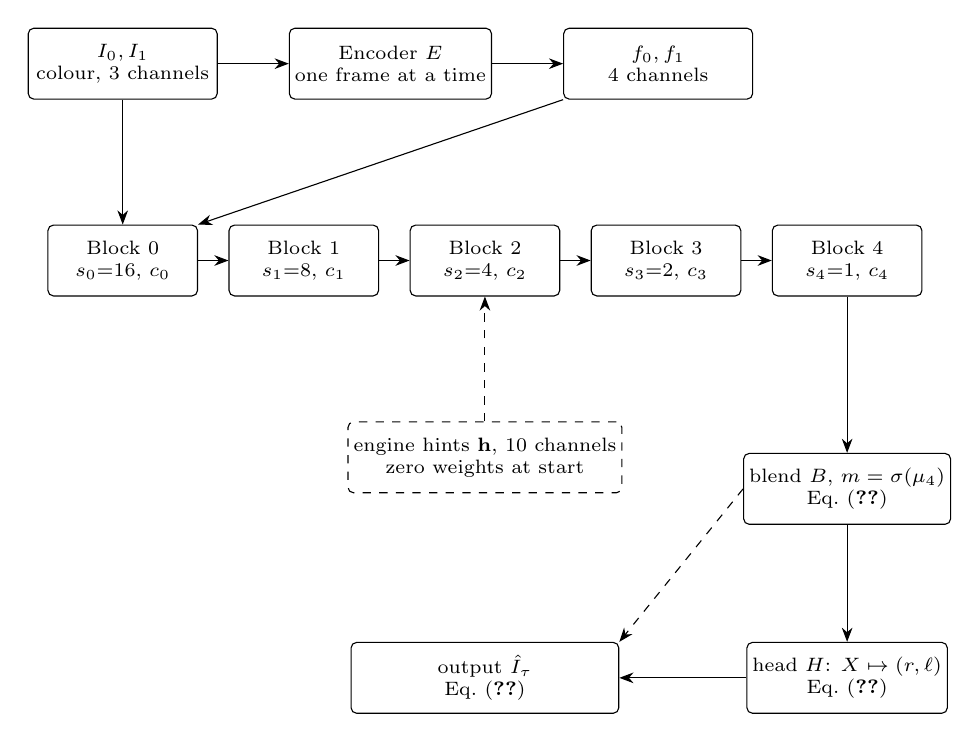
\begin{tikzpicture}[font=\scriptsize, box/.style={draw, rounded corners=2pt, align=center, minimum height=9mm, minimum width=19mm, inner sep=2pt},
  dashbox/.style={box, dashed}, arr/.style={-{Stealth[length=1.8mm]}}]
\node[box, minimum width=24mm] (in) at (0,0) {$I_0,I_1$\\colour, 3 channels};
\node[box, minimum width=24mm] (enc) at (3.4,0) {Encoder $E$\\one frame at a time};
\node[box, minimum width=24mm] (feat) at (6.8,0) {$f_0,f_1$\\4 channels};
\node[box] (b0) at (0,-2.5) {Block 0\\$s_0{=}16$, $c_0$};
\node[box] (b1) at (2.3,-2.5) {Block 1\\$s_1{=}8$, $c_1$};
\node[box] (b2) at (4.6,-2.5) {Block 2\\$s_2{=}4$, $c_2$};
\node[box] (b3) at (6.9,-2.5) {Block 3\\$s_3{=}2$, $c_3$};
\node[box] (b4) at (9.2,-2.5) {Block 4\\$s_4{=}1$, $c_4$};
\node[dashbox, minimum width=24mm] (hint) at (4.6,-5.0) {engine hints $\mathbf h$, 10 channels\\zero weights at start};
\node[box, minimum width=24mm] (blend) at (9.2,-5.4) {blend $B$, $m=\sigma(\mu_4)$\\Eq.~\eqref{eq:fgm-blend}};
\node[box, minimum width=24mm] (head) at (9.2,-7.8) {head $H$: $X\mapsto(r,\ell)$\\Eq.~\eqref{eq:fgm-head-in}};
\node[box, minimum width=34mm] (out) at (4.6,-7.8) {output $\hat I_\tau$\\Eq.~\eqref{eq:fgm-out}};
\draw[arr] (in.east) -- (enc.west);
\draw[arr] (enc.east) -- (feat.west);
\draw[arr] (in.south) -- (b0.north);
\draw[arr] (feat.south west) -- (b0.north east);
\draw[arr] (b0.east) -- (b1.west);
\draw[arr] (b1.east) -- (b2.west);
\draw[arr] (b2.east) -- (b3.west);
\draw[arr] (b3.east) -- (b4.west);
\draw[arr, dashed] (hint.north) -- (b2.south);
\draw[arr] (b4.south) -- (blend.north);
\draw[arr] (blend.south) -- (head.north);
\draw[arr] (head.west) -- (out.east);
\draw[arr, dashed] (blend.west) -- (out.north east);
\end{tikzpicture}
\caption{IFNet with the head. The encoder runs once per frame. Block $k$ takes the warped frames and features under the current flow, the previous mask and features, and $\tau$ (Eqs.~\eqref{eq:fgm-block0} and \eqref{eq:fgm-blockk}), and it outputs $\Delta_k$, $\mu_k$ and $\varphi_k$ (Eq.~\eqref{eq:fgm-blockout}). Engine hints enter every block through zero-initialised weights (\cref{sec:fgm-hints}). Block 4 gives the blend $B$, and the half-resolution head gives the residual $r$ and the UI logit, which form the output (Eqs.~\eqref{eq:fgm-head-in} and \eqref{eq:fgm-out}). The block scales and widths shown are those of the \tier{high} tier}\label{fig:fgm-ifnet}
\end{figure}

\subsection{RIFE 4.26 weights and the reproduction check}\label{sec:fgm-weights}

The weights are RIFE 4.26's archive, published in the author's Hugging Face repository. The downloader checks the SHA-256 hash of the archive and then of the \texttt{flownet.pkl} file inside it, and it loads the state dictionary with \texttt{weights\_only=True}, so the file cannot run code. The parameter names and shapes of the \tier{high} tier equal RIFE's, so every tensor is loaded by name. Where a tensor of a tier is smaller than its RIFE counterpart, the loader copies the leading slice along every dimension, the minimum of the two sizes. Where RIFE has more residual blocks than the tier, the first $n$ blocks are copied and the rest are ignored. Tensors that have no RIFE counterpart keep their initialisation, and the hint input columns keep their zero weights (\cref{sec:fgm-hints}). For the \tier{high} tier the loader reports 153 tensors copied exactly and 5 copied with a slice. The five sliced tensors are the first convolutions of the blocks, which are widened by the 10 hint channels, and no tensor is missing.

\emph{Reproduction check.} The check compares the \tier{high} tier with RIFE 4.26's own network code, the \texttt{IFNet\_HDv3} module of the archive, on the same inputs and with no engine data. RIFE's warp function is not in the archive, so the check recreates it with the grid convention of \cref{eq:fgm-warp}. The inputs are a random $8\times12$ image upsampled bicubically to $128\times192$ as $I_0$, and $I_0$ rolled by $(2,5)$ pixels as $I_1$, at $\tau=1/2$. The repository's check accepts a difference below $10^{-4}$ between the blend $B$ and RIFE's merged output in float32 on the CPU, and the agreement it measures is below $10^{-5}$. It also checks that the residual head and the hints add nothing at initialisation (\cref{sec:fgm-hints,sec:fgm-output}). The check tests the network code against RIFE's network code. It does not test the warp against RIFE's own kernel, and it does not test the delivered output of the generator, which differs from the blend (\cref{sec:fgm-output}).

\subsection{Tiers and channel-slice inheritance}\label{sec:fgm-tiers}

\Cref{tab:fgm-tiers} lists the four tiers. The \tier{high} tier has RIFE's widths, residual depth and block layout, and it is the one that starts from RIFE 4.26's network. The smaller tiers are narrower, with fewer residual blocks per block and a narrower head. Each tier is the generator of \cref{eq:fgm-task} with its own widths, residual depth, head width and flow line limit.

\begin{table}[!htbp]
\caption{Frame-generation tiers. Widths are the channel counts of blocks 0 to 4, $n$ the residual blocks per block, $c_h$ the head width, $L$ the flow line limit of \cref{eq:fgm-scale}, and GMAC the multiply-accumulates per 1080p output frame (every convolution, warps excluded), with flow at the scale the tier uses at 1080p}\label{tab:fgm-tiers}
\begin{tabular*}{\textwidth}{@{\extracolsep\fill}lllrrrr}
\toprule
Tier & Widths $c_0,\dots,c_4$ & $n$ & $c_h$ & $L$ & Params & GMAC \\
\midrule
\tier{igpu} & 64, 48, 32, 24, 16 & 3 & 12 & 576 & \Res{fg.model_tiers.igpu.params} & \Res{fg.model_tiers.igpu.gmac_per_1080p_frame} \\
\tier{low} & 96, 64, 48, 32, 16 & 4 & 16 & 576 & \Res{fg.model_tiers.low.params} & \Res{fg.model_tiers.low.gmac_per_1080p_frame} \\
\tier{mid} & 128, 96, 64, 48, 24 & 6 & 24 & 1152 & \Res{fg.model_tiers.mid.params} & \Res{fg.model_tiers.mid.gmac_per_1080p_frame} \\
\tier{high} & 192, 128, 96, 64, 32 & 8 & 32 & 1152 & \Res{fg.model_tiers.high.params} & \Res{fg.model_tiers.high.gmac_per_1080p_frame} \\
\bottomrule
\end{tabular*}
\end{table}

\emph{Channel-slice inheritance.} A smaller tier starts from RIFE's weights through the copy rule of \cref{sec:fgm-weights}. The narrower tensors take the leading channels of RIFE's tensor along each channel dimension, so the output channels of a block and the input channels of the next layer keep the same ordering. For the \tier{igpu} tier the loader reports 13 tensors with exact shapes and 70 sliced, for the \tier{low} tier 13 and 85, and for the \tier{mid} tier 13 and 115, with no missing tensor. The head has no RIFE counterpart, so it starts from its initialisation in every tier. The inheritance is a heuristic. Nothing forces RIFE's leading channels to be the best subset for a narrower network, and the ablation without inheritance (\cref{sec:fgm-ablate}) is the test of how much it matters.

\subsection{Flow-resolution caps and their cost}\label{sec:fgm-caps}

Estimating flow at full resolution is the most expensive part of the network, so every tier caps the number of image lines at which it estimates flow. A frame of height $H$ lines is halved until it fits under the tier's limit $L$, as RIFE's own scale argument allows:
\begin{equation}
s(H)=2^{-j^\ast},\qquad j^\ast=\min\big\{\,j\in\mathbb N_0:\,H\,2^{-j}\le L\,\big\},\label{eq:fgm-scale}
\end{equation}
with $L=576$ lines for the \tier{igpu} and \tier{low} tiers and $L=1152$ lines for the \tier{mid} and \tier{high} tiers. At 1080 lines the \tier{igpu} and \tier{low} tiers therefore estimate flow at $s=1/2$ (540 lines), and the \tier{mid} and \tier{high} tiers at $s=1$. The 256-pixel training crops and video up to 576 lines keep full-resolution flow in every tier. The frames are downsampled by $s$ before the encoder and the blocks, the flow hints are multiplied by $s$, and the flows that come out are upsampled and multiplied by $1/s$ to return to pixels. The head, the warps and the output stay at full resolution.

The convolution cost of the encoder and the blocks scales with the pixel count of the frames they see, so it scales with $s^2$. The head does not change. \Cref{tab:fgm-cap} gives the consequence at 1080p, counted with the same hooks as \cref{tab:fgm-tiers}. The cap removes more than half of the flow-path cost of the \tier{igpu} and \tier{low} tiers. For the \tier{low} tier the head is about a third of the capped cost, so the head matters most for the smallest tiers.

\begin{table}[!htbp]
\caption{Cost per 1080p generated frame of the tiers with the flow cap of \cref{eq:fgm-scale} and with full-resolution flow (GMAC, warps excluded). The encoder column counts both real frames, as the repository's tier table does, so one encoder pass is half of it. The head is the residual head of \cref{sec:fgm-output}}\label{tab:fgm-cap}
\begin{tabular*}{\textwidth}{@{\extracolsep\fill}lrrrrr}
\toprule
Tier & Flow scale & Capped total & Full-flow total & Encoder (two frames) & Head \\
\midrule
\tier{igpu} & \Res{fg.model_tiers.igpu.flow_scale_1080p} & \Res{fg.model_tiers.igpu.gmac_per_1080p_frame} & 20.4 & \Res{fg.model_tiers.igpu.gmac_per_frame_encoder} & 2.9 \\
\tier{low} & \Res{fg.model_tiers.low.flow_scale_1080p} & \Res{fg.model_tiers.low.gmac_per_1080p_frame} & 25.5 & \Res{fg.model_tiers.low.gmac_per_frame_encoder} & 4.5 \\
\tier{mid} & \Res{fg.model_tiers.mid.flow_scale_1080p} & \Res{fg.model_tiers.mid.gmac_per_1080p_frame} & 44.3 & \Res{fg.model_tiers.mid.gmac_per_frame_encoder} & 8.5 \\
\tier{high} & \Res{fg.model_tiers.high.flow_scale_1080p} & \Res{fg.model_tiers.high.gmac_per_1080p_frame} & 76.7 & \Res{fg.model_tiers.high.gmac_per_frame_encoder} & 13.8 \\
\bottomrule
\end{tabular*}
\end{table}

\subsection{Engine hints and their zero initialisation}\label{sec:fgm-hints}

When an engine provides data, the generator receives them as extra input channels of every IFNet block. \Cref{tab:fgm-hints} lists the ten channels in the order of the code. The signal channels are multiplied by their availability, so an absent signal contributes zero, and the flags tell the network which case it is in.

\emph{Motion priors.} If a point moves with constant velocity between $I_0$ and $I_1$, its displacement from $I_1$ to $I_0$ is $M_1$, and at time $\tau$ its displacement to $I_0$ is $\tau M_1$ and to $I_1$ is $(\tau-1)M_1$. The priors are exact only for linear motion, so the network has to learn when to trust them. The zero initialisation below lets it start from a working point.

\emph{Camera-only flow and late latching.} The camera flow $C$ is the displacement that the camera motion alone induces on the static background, from the target pixel to $I_1$. Let $A_t$ be the background affine map from screen to texture at time $t$ (\cref{sec:data-synth}), with normalised coordinates $x\in[-1,1]^2$. Then
\begin{equation}
C(x)=\tfrac{P}{2}\big(A_1^{-1}(A_\tau(x))-x\big),
\end{equation}
where $P$ is the frame size in pixels, so that $P/2$ converts normalised displacements to pixels for a $P\times P$ frame. Object motion is absent from $C$. At display time an engine knows the camera pose of the frame it is about to show, so the pose can be latched just before generation and supplied as this prior. In the synthetic training the prior uses the exact background trajectory at $\tau$. For real video the camera availability is zero, so the prior is never present.

\emph{Depth.} The depth channel is the inverse depth of $I_1$ normalised by its median, $d_1=1/(1+d/\operatorname{median}(d))$, so that a pixel at the median depth has the value one half. It is defined only for the synthetic renderer, where the depth is exact.

\emph{Availability.} Each availability flag is set per sample, and the signal channels are multiplied by the flags. Withholding a signal in training is therefore the same as an engine that does not provide it. The withholding rates are in \cref{tab:fgm-probs}.

\begin{table}[!htbp]
\caption{Sampling probabilities of the frame-generation training data, with the configuration names used in the saved files, or the constant in the code where no configuration name exists}\label{tab:fgm-probs}
{\footnotesize\begin{tabular*}{\textwidth}{@{\extracolsep\fill}lrl}
\toprule
Quantity & Value & Configuration or constant \\
\midrule
Real share of each GPU batch & \Res{fg.config.cfg.p_real} (19 of 48) & \texttt{p\_real} \\
Extrapolation, both sample kinds & \Res{fg.config.cfg.p_extrap} & \texttt{p\_extrap} \\
Random $\tau$ for synthetic interpolation & \Res{fg.config.cfg.p_tau} & \texttt{p\_tau}, $\tau\sim U[0.15,0.85]$ \\
Multi-frame share of real interpolation & \Res{fg.config.cfg.p_mfg} & \texttt{p\_mfg} \\
Camera reversal & \Res{fg.config.cfg.p_flip} & \texttt{p\_flip} \\
Scene cut & \Res{fg.config.cfg.p_cut} & \texttt{p\_cut} \\
UI overlay & \Res{fg.config.cfg.p_ui} & \texttt{p\_ui} \\
Menu, given a UI overlay & \Res{fg.config.cfg.p_menu} & \texttt{p\_menu} \\
Withhold motion vector (synthetic) & \Res{fg.config.cfg.p_drop_mv} & \texttt{p\_drop\_mv} \\
Withhold motion vector (real) & \Res{fg.config.cfg.p_drop_mv_real} & \texttt{p\_drop\_mv\_real} \\
Withhold depth (synthetic) & 0.30 & default argument in \texttt{set\_availability} \\
Withhold camera prior (extrapolation) & 0.20 & constant in \texttt{set\_availability} \\
UI slot filled / tile changed at $t=1$ & 0.70 / 0.30 & \texttt{ui\_layer} \\
\bottomrule
\end{tabular*}}
\end{table}

\paragraph{Zero-initialisation argument.} Let $W^{\mathbf h}_k$ be the weights of the first convolution of block $k$ that multiply the hint channels, and let every other weight of the \tier{high} tier equal RIFE's. The claim is that with $W^{\mathbf h}_k=0$ for every $k$, the blend $B$ does not depend on $\mathbf h$ and equals RIFE 4.26's blend. The argument is by induction over the blocks. Block 0 receives the same input as in RIFE, so its first convolution computes $z=W_x*x+W^{\mathbf h}_0*\mathbf h+b$ with $W^{\mathbf h}_0=0$, which equals RIFE's pre-activation $W_x*x+b$. The later layers of the block see only $z$, so the block outputs $(\Delta_0,\mu_0,\varphi_0)$ equal RIFE's. The induction step is the same for block $k$, because the warps and features that enter block $k$ are functions of the earlier outputs only. The blend of \cref{eq:fgm-blend} is then RIFE's blend. The head adds nothing at initialisation, because its last layer has zero weights and bias $(0,0,0,-4)$ (\cref{sec:fgm-output}). The gradient with respect to the hint columns is $\partial L/\partial W^{\mathbf h}_k=\sum_p \delta_k(p)\,\mathbf h(p)^{\top}$, summed over the sampled positions $p$, where $\delta_k$ is the gradient at the first-layer output. This is not zero when the hints are non-zero and the loss is sensitive to block $k$, so the hint columns leave zero at the first update. The fresh model therefore reproduces RIFE's blend, and then learns from the engine data.

\subsection{Head, UI weight and output}\label{sec:fgm-output}

The head turns the warped frames into a residual colour and a UI logit. Its input is the full-resolution stack of the two real frames, the two warps under the final flow, the blend weight and the last features:
\begin{equation}
X=\big[I_0,\,I_1,\,\mathcal W(I_0,F_4^0),\,\mathcal W(I_1,F_4^1),\,m,\,\varphi_4\big]\qquad(21\text{ channels}).\label{eq:fgm-head-in}
\end{equation}
A stride-2 $3\times3$ convolution with $c_h$ channels and LeakyReLU, two residual blocks at half resolution with the design of \cref{sec:fgm-ifnet}, and a $4\times4$ transposed convolution with stride 2 give four output channels, $(r,\ell)=H(X)$. Here $r$ is the residual colour and $\ell$ the UI logit. The head starts with a zero transposed-convolution weight and bias $(0,0,0,-4)$, so $r=0$ and $\ell=-4$ at initialisation, and the UI weight $u=\sigma(\ell)$ is about $0.018$. The output is
\begin{equation}
\hat I_\tau=u\odot I_1+(1-u)\odot\big(B+r\big),\qquad u=\sigma(\ell),\label{eq:fgm-out}
\end{equation}
with the blend $B$ of \cref{eq:fgm-blend}. This is \cref{M-eq:fg} of the article.

The UI weight is a soft mask in $[0,1]$, not a hard classification. Training pushes $u$ towards one on HUD, subtitle and menu pixels, where the UI mask of \cref{eq:fgm-ui-bce} is one, and towards zero elsewhere, so that those pixels come from the newest real frame $I_1$. The starting value means that a fresh model already mixes a small fraction of $I_1$ into every pixel. The delivered output of a fresh model therefore differs from the blend by $u\odot(I_1-B)$, which is small but not zero. This is why the reproduction check of \cref{sec:fgm-weights} compares the blend and not the output.

Evaluation clamps the output to $[0,1]$ before computing metrics. Training does not clamp, so the loss sees the unclamped output.

\emph{UI layer compositing.} When an engine renders the HUD separately from the scene, it can supply HUD-less real frames and the UI layer for the newest state, as premultiplied colour $c$ and alpha $\alpha$. The generator then runs on the HUD-less frames, and the displayed frame is $\hat I_\tau(1-\alpha)+c$. In the design this is applied to every displayed frame of the layer's sequence. The evaluation applies it to the generated frame only (\cref{sec:fgm-test}).

\subsection{Per-frame encoder reuse}\label{sec:fgm-encoder}

The encoder of \cref{eq:fgm-enc} depends on one frame, so a running sequence can encode each real frame once and reuse its features. The IFNet forward pass takes optional precomputed features for this, but no caller in the repository passes them. Training, evaluation and the exported graph all encode both frames (\cref{sec:fgm-export}).

The cost accounting follows from this. The encoder column of \cref{tab:fgm-cap} counts two frames, so one pass per real frame is half the column. With one generated frame per real frame, reuse replaces two encoder passes per generated frame by one.

\subsection{Scene-cut gate}\label{sec:fgm-cut}

\UnderRevision{} The gate decides when the generator should not generate. When two real frames look as if a scene cut lies between them, it outputs the newest real frame $I_1$ instead of $\hat I_\tau$. The repository marks this stage as a known weakness. Its thresholds are calibrated on synthetic adjacent pairs only, so the calibration does not cover real content or wider frame gaps.

The score combines a colour-distribution distance, which needs no motion, with a motion-compensated difference, which is used when $M_1$ is available. Let $Y(x)=(16+65.481R(x)+128.553G(x)+24.966B(x))/255$ be the limited-range luma of an RGB pixel with values in $[0,1]$, and let $h(I)\in\mathbb R^{32}$ be the fraction of pixels whose luma falls in each of 32 equal bins of $[0,1]$. The histogram distance and the motion-compensated difference are
\begin{align}
d_{\rm h}(I_0,I_1)&=\tfrac12\big\|h(I_0)-h(I_1)\big\|_1\in[0,1],\label{eq:fgm-hist}\\
d_{\rm m}(I_0,I_1,M_1)&=\frac{1}{3HW}\sum_{x,c}\big|I_1(x,c)-\mathcal W(I_0,M_1)(x,c)\big|.\label{eq:fgm-hist-m}
\end{align}
The two scores are
\begin{equation}
S_{\rm mv}=d_{\rm h}+2\,d_{\rm m},\qquad S_0=d_{\rm h},\label{eq:fgm-score}
\end{equation}
and the gate is
\begin{equation}
g=\begin{cases}\mathbf 1[S_{\rm mv}>\theta_{\rm mv}] & \text{if }a_{\rm mv}=1,\\ \mathbf 1[S_0>\theta_0] & \text{otherwise,}\end{cases}\label{eq:fgm-gate}
\end{equation}
where $\mathbf 1[\cdot]$ is one when its condition holds and zero otherwise. Without motion vectors the histogram distance alone is used, because a raw frame difference would read ordinary fast motion as a cut. The gate lives in the evaluation code, and it is not part of the exported graph.

\emph{Calibration.} Each threshold is set separately on synthetic pairs, so that continuous motion is a false alarm on about one pair in a hundred.
\begin{enumerate}
\item Draw four batches of up to 64 validation stills. For each batch, generate interpolation pairs at $\tau=1/2$ with motion from all four speed classes, no camera reversal and no UI, and with a cut probability of one half. Each pair is labelled cut or continuous. This gives 256 pairs, about half of them cuts.
\item Compute $S_{\rm mv}$ with the exact motion vector and $S_0$ for every pair.
\item For each score, sort the scores of the continuous pairs in ascending order and take the element at 0-based index $\lfloor0.99(n-1)\rfloor$, where $n$ is the number of continuous pairs. This element is the threshold $\theta$.
\item Report the detection rate, which is the share of cut pairs whose score exceeds $\theta$.
\end{enumerate}
The calibrated values are part of the results (\cref{sec:fgr}). When the gate fires, the output is the newest real frame,
\begin{equation}
\hat I_\tau\quad\leftarrow\quad I_1\qquad\text{if } g=1.\label{eq:fgm-gated}
\end{equation}

\subsection{Latency model and pacing}\label{sec:fgm-pacing}

\UnderRevision{} The latency numbers are timed on one data-centre GPU in eager PyTorch, and the pacing model is a simulation with assumed scheduling. The latency terms are those of \cref{sec:bg-latency}. The repository marks in-engine latency on target hardware as not measured. The model therefore answers what frame generation does to the displayed rate and to two latencies, under the stated assumptions.

The model is a discrete-event simulation of a GPU-bound loop with just-in-time CPU scheduling, in which the CPU starts each frame's work so that the GPU never queues frames, on a variable-refresh display. Its parameters are in \cref{tab:fgm-pacing}. The modes are \emph{native} (no generation), \emph{interpolation} (a generated frame between two real frames, with the newer real frame held), \emph{extrapolation} (a generated frame after the newest real frame, with nothing held) and \emph{extrapolation with late latching} (extrapolation whose camera is sampled just before generation).

\begin{table}[!htbp]
\caption{Parameters of the pacing model, as set in the simulation code and the notebook. The generation time $T_{\rm gen}$ is the measured one-generated-frame time of the \tier{low} tier at 1080p (\cref{sec:fgr}). The temporal super-resolution time $T_{\rm sr}$ is zero, because this pacing run has no such stage}\label{tab:fgm-pacing}
\begin{tabular*}{\textwidth}{@{\extracolsep\fill}lll}
\toprule
Symbol & Value & Meaning \\
\midrule
$R_0$ & 33.3, 25.0, 16.7\,ms & base render time per real frame (30, 40 and 60 fps renders) \\
$C_{\rm cpu}$ & 4.0\,ms & CPU time per frame before rendering starts \\
$c_v$ & 0.08 & log-normal spread of the render time \\
$T_{\rm pres}$ & 1.0\,ms & present time \\
$T_{\rm sr}$ & 0 & temporal super-resolution time \\
$T_{\rm gen}$ & measured & frame generation time per generated frame \\
$N$ & 2000 & simulated real frames per run \\
seed & 0 & random seed of the render times \\
\bottomrule
\end{tabular*}
\end{table}

The simulation runs as follows.
\begin{enumerate}
\item For each real frame $j=1,\dots,N$, draw the render time $R_j=R_0\exp(c_v z_j)$, where $z_j$ is standard normal.
\item Set the GPU time $g_j=R_j+T_{\rm sr}+T_{\rm gen}\,\mathbf 1[\text{mode}\neq\text{native}]$ and the frame period $\pi_j=\max(C_{\rm cpu},g_j)$.
\item Let $t_j$ be the time of the input sample, which is the current simulation time.
\item Set the time at which the rendered real frame is ready, $a_j=t_j+C_{\rm cpu}+R_j+T_{\rm sr}$.
\item In the \emph{native} mode, display the real frame at $p^{\rm r}_j=a_j+T_{\rm pres}$.
\item In the \emph{interpolation} mode, display the generated frame at $p^{\rm g}_j=a_j+T_{\rm gen}+T_{\rm pres}$, and hold the real frame until $p^{\rm r}_j=p^{\rm g}_j+\pi_j/2$.
\item In the \emph{extrapolation} mode, display the real frame at $p^{\rm r}_j=a_j+T_{\rm pres}$, and the generated frame at $p^{\rm g}_j=p^{\rm r}_j+\pi_j/2$.
\item In the \emph{extrapolation with late latching} mode, proceed as in step 7, and sample the camera of the generated frame at $t^{\rm cam}_j=p^{\rm g}_j-T_{\rm gen}-T_{\rm pres}$, the moment generation starts.
\item Record the displayed frames and the latency samples below, and advance the simulation time by $t\leftarrow t+\pi_j$.
\end{enumerate}
The rates are computed on the displayed times after the first tenth of the displayed sequence, so that start-up does not count. With $\Delta_i$ the gaps between consecutive displayed times, the displayed frame rate and the gap variation are $\mathrm{fps}=1000/\overline\Delta$ and $\mathrm{CV}=\operatorname{sd}(\Delta)/\overline\Delta$, in milliseconds for $\Delta$.

Three latencies are reported. The game input latency is the time from an input sample to the display of the real frame that reflects it, averaged over the real frames of the run,
\begin{equation}
L_{\rm game}=\operatorname{mean}_j\big(p^{\rm r}_j-t_j\big).\label{eq:fgm-lat-game}
\end{equation}
The camera latency is the same kind of time, measured to each displayed frame that counts as reflecting the camera. In the code a native frame counts with its real display. An interpolated frame counts with its generated display only, on the assumption that the generated frame already moves half way toward the camera of the newer frame. An extrapolated frame counts with both its real and its generated display, and with late latching the generated display is measured from $t^{\rm cam}_j$:
\begin{equation}
L_{\rm cam}=\begin{cases}\operatorname{mean}_j\big(p^{\rm r}_j-t_j\big) & \text{native},\\[2pt] \operatorname{mean}_j\big(p^{\rm g}_j-t_j\big) & \text{interpolation},\\[2pt] \tfrac12\Big(\operatorname{mean}_j\big(p^{\rm r}_j-t_j\big)+\operatorname{mean}_j\big(p^{\rm g}_j-t_j\big)\Big) & \text{extrapolation},\\[2pt] \tfrac12\Big(\operatorname{mean}_j\big(p^{\rm r}_j-t_j\big)+\operatorname{mean}_j\big(p^{\rm g}_j-t^{\rm cam}_j\big)\Big) & \text{late latching.}\end{cases}\label{eq:fgm-lat-cam}
\end{equation}
The content age averages the time from the input sample to every displayed frame, real or generated,
\begin{equation}
A=\operatorname{mean}_p\big(p-t\big)\quad\text{over all displayed frames }p.\label{eq:fgm-lat-age}
\end{equation}
Each latency is also reported at its 95th percentile over the samples.

The arithmetic estimate of a network's time at a sustained throughput $F$ in TFLOPS, is $T_{\rm est}=2G/F$ milliseconds, for a frame that costs $G$ GMAC, because one multiply-accumulate is two floating-point operations. The repository uses $F=4$ TFLOPS for an assumed integrated GPU. The estimate scales the GMAC with pixel count, so at 1440p it ignores the flow cap of \cref{eq:fgm-scale}.

\begin{figure}[!htbp]
\centering
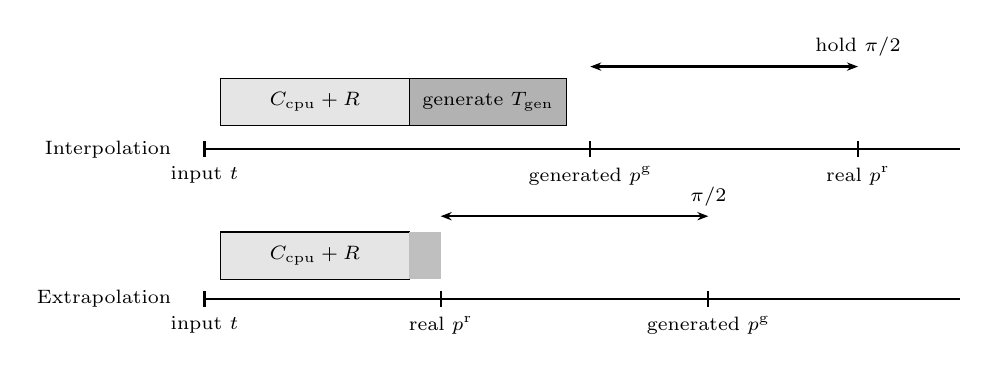
\begin{tikzpicture}[font=\scriptsize, x=1cm, y=1cm,
  tick/.style={thick},
  lab/.style={font=\scriptsize, align=center},
  bar/.style={draw, minimum height=6mm, inner sep=1pt}]
\node[anchor=east, lab] at (-0.3,1.9) {Interpolation};
\draw[thick] (0,1.9) -- (9.6,1.9);
\node[bar, fill=black!10, minimum width=2.4cm] at (1.4,2.5) {$C_{\rm cpu}+R$};
\node[bar, fill=black!30, minimum width=2.0cm] at (3.6,2.5) {generate $T_{\rm gen}$};
\draw[tick] (0,1.8) -- (0,2.0);
\node[lab, below] at (0,1.8) {input $t$};
\draw[tick] (4.9,1.8) -- (4.9,2.0);
\node[lab, below] at (4.9,1.8) {generated $p^{\rm g}$};
\draw[tick] (8.3,1.8) -- (8.3,2.0);
\node[lab, below] at (8.3,1.8) {real $p^{\rm r}$};
\draw[{Stealth[length=1.4mm]}-{Stealth[length=1.4mm]}, thick] (4.9,2.95) -- (8.3,2.95) node[above, lab] {hold $\pi/2$};
\node[anchor=east, lab] at (-0.3,0.0) {Extrapolation};
\draw[thick] (0,0.0) -- (9.6,0.0);
\node[bar, fill=black!10, minimum width=2.4cm] at (1.4,0.55) {$C_{\rm cpu}+R$};
\fill[black!25] (2.6,0.25) rectangle (3.0,0.85);
\draw[tick] (0,-0.1) -- (0,0.1);
\node[lab, below] at (0,-0.1) {input $t$};
\draw[tick] (3.0,-0.1) -- (3.0,0.1);
\node[lab, below] at (3.0,-0.1) {real $p^{\rm r}$};
\draw[tick] (6.4,-0.1) -- (6.4,0.1);
\node[lab, below] at (6.4,-0.1) {generated $p^{\rm g}$};
\draw[{Stealth[length=1.4mm]}-{Stealth[length=1.4mm]}, thick] (3.0,1.05) -- (6.4,1.05) node[above, lab] {$\pi/2$};
\end{tikzpicture}
\caption{Timeline of one input sample in the two generation modes, schematic and not to scale. In interpolation the generated frame needs the newest real frame, and the real frame is held for half a period, so it is shown after the generated frame. In extrapolation the real frame is shown as soon as it is rendered, and the generated frame follows half a period later, with the generation time $T_{\rm gen}$ inside that period. The grey bar at $T_{\rm pres}$ in the extrapolation row is the present time. The labels are the symbols of \cref{tab:fgm-pacing}}\label{fig:fgm-timeline}
\end{figure}

\cref{fig:fgm-timeline} shows the two modes. Interpolation adds $T_{\rm gen}$ to the time of the generated frame and delays the real frame by half a period. Extrapolation adds no delay to the real frame and adds half a period to the generated frame, which is shown after the real frame.

\subsection{Training samples}\label{sec:fgm-samples}

In the main stages each of the two GPUs takes its own batch of 48 samples per step, under distributed data parallel training. A batch holds 19 real quads and 29 synthetic samples, since the real share \Res{fg.config.cfg.p_real} of 48 rounds to 19, drawn at random without replacement from the caches. Still crops are $512\times512$ pixels cut from the textures of \cref{sec:data-synth}, and quads are four frames of $256\times256$ pixels from the sequence sources of \cref{sec:data}, both after the random downscale of \cref{sec:data}. The cache sizes are in \cref{sec:fgr}.

\paragraph{Synthetic samples.} Each synthetic sample is one scene of the renderer of \cref{sec:data-synth}, rendered at $256\times256$ pixels with four anti-aliasing samples per pixel for $I_0$, $I_1$ and the target. The background is one still. The foreground is the still of the neighbouring sample in the batch, visible through a procedural alpha mask in 85 percent of samples, and a flat colour in 25 percent of samples. The construction of one sample is as follows.
\begin{enumerate}
\item Draw the camera reversal with probability \Res{fg.config.cfg.p_flip}. A reversal reverses the camera velocity after $t=1$.
\item Draw extrapolation with probability \Res{fg.config.cfg.p_extrap}. If it is extrapolation, set $\tau=1.5$. Otherwise set $\tau=1/2$, or with probability \Res{fg.config.cfg.p_tau} draw $\tau$ uniformly from $[0.15,0.85]$.
\item Render $I_0$ at $t=0$, $I_1$ at $t=1$ and the target at $t=\tau$.
\item Compute the exact motion vector $M_1$, which is the flow from $I_1$ to $I_0$, the exact flows $F_{\tau\to0}$ and $F_{\tau\to1}$ with their validity masks (visible and inside the view), the camera flow $C$ and the inverse depth $d_1$.
\item Draw a scene cut with probability \Res{fg.config.cfg.p_cut}. A cut replaces $I_1$, $M_1$ and $d_1$ by those of the neighbouring sample, sets the target to the replaced $I_1$, and sets the validity masks to zero.
\item Draw UI overlays with probability \Res{fg.config.cfg.p_ui}. Four UI slots are each filled with probability 0.7 by a tile from a bank of 256 text, bar and crosshair tiles of $160\times28$ pixels, and 30 percent of the filled slots change their tile at $t=1$. A full-screen menu panel of alpha 0.6 and colour 0.05 is drawn with probability \Res{fg.config.cfg.p_menu} given a UI overlay, which is 1.5 percent of all samples. The tiles are alpha-composited into $I_0$ with the state at $t=0$, into $I_1$ with the state at $t=1$, and into the target with the state at $t=1$. The UI mask is the maximum of the two alphas.
\item Withhold the signals according to \cref{tab:fgm-probs}, and set the camera availability to zero for every interpolation sample.
\end{enumerate}

\paragraph{Real quads.} Each real sample is a window of four consecutive frames from one of the sequence sources of \cref{sec:data}, decoded and cut to $256\times256$ pixels. The window is flipped horizontally and vertically with probability one half each, and its flow fields are flipped with it, with the vector components negated along each flipped axis. The sample then takes one of three forms.
\begin{enumerate}
\item With probability \Res{fg.config.cfg.p_extrap}, extrapolation: $I_0=k$, $I_1=k+2$ and target $k+3$, at $\tau=1.5$.
\item Otherwise, with probability \Res{fg.config.cfg.p_mfg}, multi-frame generation: $I_0=k$, $I_1=k+3$, and the target is $k+1$ or $k+2$ with equal probability, at $\tau=1/3$ or $2/3$.
\item Otherwise interpolation: $I_0=k$, $I_1=k+2$ and target $k+1$, at $\tau=1/2$.
\end{enumerate}
The flows come from the RAFT optical-flow network \cite{teed2020raft}, in the small variant that torchvision ships with its weights. The cache computes four flows per quad, $k+2\to k$, $k+1\to k$, $k+1\to k+2$ and $k+3\to k+2$, at the $256\times256$ crop size, and stores them at half resolution, in pixels of the full grid, by two-by-two average pooling. Every quad carries these four flows, including the TartanAir and Sintel quads that have exact flows in the frame decoder, because the quad cache does not use those flows. The motion vector $M_1$ is the flow $k+2\to k$. The flows $F_{\tau\to0}$ and $F_{\tau\to1}$ are $k+1\to k$ and $k+1\to k+2$ for interpolation, and $k+3\to k+2$ for extrapolation. An extrapolated sample has no label from the target to $I_0$, so its $F_{\tau\to0}$ validity is zero. A multi-frame sample has no flow label, so its $M_1$ and both flow validities are zero. A real sample has no depth and no camera prior, so its depth and camera availabilities are zero. Every pixel of a real flow is valid, because the cache computes no validity mask.

\paragraph{Availability and the plain-video case.} \Cref{tab:fgm-probs} gives the withholding rates. Synthetic samples withhold the motion vector with probability \Res{fg.config.cfg.p_drop_mv} and the depth with probability 0.3, and they keep the camera prior with probability 0.8 on extrapolation samples only. Real samples withhold the motion vector with probability \Res{fg.config.cfg.p_drop_mv_real} when a flow label exists, and they never have depth or a camera prior. The validation batches are fixed, with \Res{fg.config.cfg.val_bs} stills and \Res{fg.config.cfg.val_bs} quads in each of \Res{fg.config.cfg.val_batches} batches, drawn with a seed of 54321. Each is evaluated twice, once with its availabilities and once with all of them set to zero, which is plain video.

\subsection{Training objective}\label{sec:fgm-loss}

The objective is a weighted sum of six terms, with a unit weight on the first,
\begin{equation}
\mathcal L=\mathcal L_{\rm pix}+0.5\,\mathcal L_{\rm cen}+0.1\,\mathcal L_{\rm lp}+0.01\,\mathcal L_{\rm flow}+0.2\,\mathcal L_{\rm ui}+0.5\,\mathcal L_{\rm kd},\label{eq:fgm-total}
\end{equation}
where each term is a mean over the batch. \Cref{tab:fgm-loss} gives the definitions, and the paragraphs below give the formulas.

\begin{table}[!htbp]
\caption{Training losses of the frame generator, with weights and the samples to which each term applies}\label{tab:fgm-loss}
\begin{tabular*}{\textwidth}{@{\extracolsep\fill}lp{0.42\textwidth}rp{0.30\textwidth}}
\toprule
Term & Quantity & Weight & Applies to \\
\midrule
$\mathcal L_{\rm pix}$ & Charbonnier penalty, $\varepsilon=10^{-3}$ & 1 & every sample \\
$\mathcal L_{\rm cen}$ & soft census distance, $7\times7$ window & \Res{fg.config.cfg.w_census} & every sample \\
$\mathcal L_{\rm lp}$ & LPIPS with AlexNet, on the clipped output & \Res{fg.config.cfg.w_lpips} & every sample, when the package loads \\
$\mathcal L_{\rm flow}$ & flow L1 on valid pixels, weight 1 (synthetic) or 1/4 (real) & \Res{fg.config.cfg.w_flow} & every sample with flow labels \\
$\mathcal L_{\rm ui}$ & binary cross-entropy on the UI mask, positive weight 4 & \Res{fg.config.cfg.w_ui} & every sample \\
$\mathcal L_{\rm kd}$ & distillation from the \tier{high} teacher & \Res{fg.config.cfg.w_distill} & students only \\
\bottomrule
\end{tabular*}
\end{table}

\emph{Charbonnier.} With the target $I_\tau$ and the output $\hat I_\tau$, $\mathcal L_{\rm pix}=\operatorname{mean}\sqrt{(\hat I_\tau-I_\tau)^2+\varepsilon^2}$, where the mean runs over every colour value. This is a smooth form of the L1 penalty. It is a smooth edge-preserving potential of the Charbonnier family \cite{charbonnier1997deterministic}.

\emph{Census.} For a grey image $g=0.299R+0.587G+0.114B$, the census vector at pixel $x$ has one soft-ternary entry per offset $\delta$ in the $7\times7$ window $D$, which has 49 offsets including zero,
\begin{equation}
c(x,\delta)=\frac{g(x+\delta)-g(x)}{\sqrt{0.81+\big(g(x+\delta)-g(x)\big)^2}}.\label{eq:fgm-census}
\end{equation}
The census distance at a pixel is $\rho(x)=\operatorname{mean}_{\delta\in D}\,d/(0.1+d)$, with $d=\big(c_{\hat I}(x,\delta)-c_{I}(x,\delta)\big)^2$. The loss $\mathcal L_{\rm cen}$ is the mean of $\rho$ over the image with a border of three pixels removed on each side. Census distances are insensitive to brightness offsets, the property for which the census loss was introduced for unsupervised flow \cite{meister2018unflow}. The soft-ternary normalisation and the robust distance are the repository's own choices.

\emph{LPIPS.} $\mathcal L_{\rm lp}$ is the LPIPS distance with the AlexNet network and version 0.1 of its calibration weights \cite{zhang2018lpips}, applied to the output clipped to $[0,1]$ and to the target, and averaged over the batch. The weight is zero when the package does not load, and the saved configuration records that.

\emph{Flow.} The flow term is the weighted L1 error of both flows over the valid pixels,
\begin{align}
\mathcal L_{\rm flow}&=\frac{\sum_x\sum_{c}\big|\hat F_{0,c}(x)-F_{0,c}(x)\big|\,v_0(x)}{2\sum_x v_0(x)+1}\nonumber\\
&\quad+\frac{\sum_x\sum_{c}\big|\hat F_{1,c}(x)-F_{1,c}(x)\big|\,v_1(x)}{2\sum_x v_1(x)+1},\label{eq:fgm-flow}
\end{align}
where $c\in\{x,y\}$ runs over the two flow components.
where $v_i=w\,\mathrm{valid}_i$ with $w=1$ for synthetic samples and $w=1/4$ for real samples. The denominator counts the valid pixels and not their weights, so a real sample contributes a quarter of the error of a synthetic one at the same pixel error.

\emph{UI.} With $y(x)=\mathbf 1[\mathrm{ui}(x)>0.5]$ for the UI mask $\mathrm{ui}=\max(\alpha_0,\alpha_1)$ of \cref{sec:fgm-samples},
\begin{equation}
\mathcal L_{\rm ui}=-\operatorname{mean}\Big[4\,y\log\sigma(\ell)+(1-y)\log\big(1-\sigma(\ell)\big)\Big],\label{eq:fgm-ui-bce}
\end{equation}
which is the binary cross-entropy on the UI logit $\ell$, with the positive term weighted by four to up-weight the rarer UI pixels.

\emph{Distillation.} When a teacher checkpoint is given, the teacher is the \tier{high} tier with the same inputs and availabilities, run without gradients. With $\hat I^{\rm T}$ and $\hat F^{\rm T}_i$ the teacher output and flows,
\begin{equation}
\mathcal L_{\rm kd}=\operatorname{mean}\big|\hat I_\tau-\hat I^{\rm T}\big|+0.01\Big(\operatorname{mean}\big|\hat F_0-\hat F^{\rm T}_0\big|+\operatorname{mean}\big|\hat F_1-\hat F^{\rm T}_1\big|\Big).\label{eq:fgm-kd}
\end{equation}
Training a student to match a teacher's outputs in this way is distillation \cite{gou2021knowledge}. The 0.01 weight on the flows is a constant of the code, not a configuration value.

\subsection{Optimisation and schedule}\label{sec:fgm-schedule}

The optimiser is AdamW \cite{loshchilov2019adamw} with betas $(0.9,0.99)$ and weight decay \Res{fg.config.cfg.weight_decay} on all parameters. The gradient norm is clipped to \Res{fg.config.cfg.grad_clip} after unscaling. The forward pass runs under fp16 autocast with dynamic loss scaling, and the losses are computed in float32 \cite{micikevicius2018mixed}. The learning rate follows the fraction $p=t/T$ of the wall-clock budget $T$ already used. It rises linearly over the first \Res{fg.config.cfg.warmup_frac} of the budget and then decays with a cosine to a floor of $\mathrm{lr}_{\min}=10^{-6}$:
\begin{equation}
\mathrm{lr}(p)=\begin{cases}\mathrm{lr}_0\,\max(p/0.03,\,0.01) & p<0.03,\\ \mathrm{lr}_{\min}+\tfrac12(\mathrm{lr}_0-\mathrm{lr}_{\min})\big(1+\cos\pi q\big) & p\geq0.03,\end{cases}\qquad q=\frac{p-0.03}{0.97}.\label{eq:fgm-lr}
\end{equation}
A moving average of the weights, the exponential moving average (EMA), is updated after every step on the rank-0 model with decay $d_s=\min(0.999,(1+s)/(10+s))$ at step $s$, so the decay starts near zero and reaches \Res{fg.config.cfg.ema_decay}. Validation runs every $\min(8\,\mathrm{min},\max(T/6,60\,\mathrm{s}))$ and at the end of the budget. Each validation saves the latest weights, and the best weights by the selection metric, which is the mean of the PSNR with and without engine data (\cref{sec:fgm-test}). The run stops with an error after 200 consecutive steps with a non-finite loss. If a run exhausts GPU memory, it is retried once with half the batch for the rest of its budget.

Training follows two stages, listed in \cref{tab:fgm-runs}. First the \tier{high} tier is fine-tuned from RIFE 4.26 on both GPUs at a learning rate of \Res{fg.config.cfg.lr_teacher} and with no teacher, since it is the tier that starts from RIFE's network. Then the smaller tiers start from RIFE's leading slices and are trained with the full objective, including distillation from the EMA weights of the fine-tuned \tier{high} run, at a learning rate of \Res{fg.config.cfg.lr}. The \tier{low} tier, the main student, uses both GPUs. The \tier{igpu} and \tier{mid} tiers train side by side, one GPU each. The nominal budgets are those of the table, and the run scales them by one common factor below one, so that the whole pipeline fits the session. The saved configurations show the scaled budgets.

\begin{table}[!htbp]
\caption{Training runs of the frame generator, in stage order. Budgets are the nominal wall-clock times, and batches are per GPU}\label{tab:fgm-runs}
\begin{tabular*}{\textwidth}{@{\extracolsep\fill}llllrrr}
\toprule
Run & Tier & Initialisation & Distillation & Learning rate & Budget (min) & Batch \\
\midrule
\texttt{fg\_teacher} & \tier{high} & RIFE 4.26 & none & \Res{fg.config.cfg.lr_teacher} & \Res{fg.config.cfg.minutes.teacher} & 48 \\
\texttt{fg\_low} & \tier{low} & RIFE slices & \tier{high} & \Res{fg.config.cfg.lr} & \Res{fg.config.cfg.minutes.student} & 48 \\
\texttt{fg\_igpu} & \tier{igpu} & RIFE slices & \tier{high} & \Res{fg.config.cfg.lr} & \Res{fg.config.cfg.minutes.pair} & 48 \\
\texttt{fg\_mid} & \tier{mid} & RIFE slices & \tier{high} & \Res{fg.config.cfg.lr} & \Res{fg.config.cfg.minutes.pair} & 24 \\
six ablations & \tier{low} & see \cref{tab:fgm-abl} & see \cref{tab:fgm-abl} & \Res{fg.config.cfg.lr} & \Res{fg.config.cfg.minutes.ablation} & 48 \\
\bottomrule
\end{tabular*}
\end{table}

\subsection{Ablations}\label{sec:fgm-ablate}

Each ablation is a \tier{low} run with the same \Res{fg.config.cfg.minutes.ablation}-minute budget as the reference. Each changes one setting of the configuration (\cref{tab:fgm-abl}), and the ablation runs go in pairs, one run per GPU. All of them use the same wall-clock budget, so the run without distillation takes more steps, because it skips the teacher's forward pass.

\begin{table}[!htbp]
\caption{Ablations of the \tier{low} tier, with the configuration change of each relative to the reference (the saved \texttt{cfg\_abl\_*.json} files)}\label{tab:fgm-abl}
\begin{tabular*}{\textwidth}{@{\extracolsep\fill}lp{0.70\textwidth}}
\toprule
Run & Change from the reference \\
\midrule
\texttt{abl\_reference} & none, so distillation from the \tier{high} run and UI training are on \\
\texttt{abl\_no\_ui\_training} & no HUD, subtitle or menu overlays in training, and UI loss weight zero \\
\texttt{abl\_no\_motion\_prior} & motion vector and camera availability forced to zero in training (depth kept) \\
\texttt{abl\_extrap\_only} & every training sample is an extrapolation ($p_{\rm extrap}=1$) \\
\texttt{abl\_no\_distillation} & no teacher, so $\mathcal L_{\rm kd}$ is absent \\
\texttt{abl\_no\_inheritance} & no RIFE weights, so the IFNet starts from the default initialisation \\
\bottomrule
\end{tabular*}
\end{table}

The \texttt{abl\_no\_motion\_prior} model is evaluated without any engine data in both modes, because its training never supplied the motion vector or the camera prior. Validation scores are not compared across ablations, which share only the test suites (\cref{sec:fgm-test}).

\subsection{Fusion and ONNX export}\label{sec:fgm-export}

The re-parameterisation fusion of the temporal super-resolution network does not apply to the generator, since it has no such blocks. Fusion here is a copy in evaluation mode, and the check that fused and unfused outputs agree holds by construction. The fused weights are stored, and their fp16 copies are used for timing.

The export wrapper takes the two real frames, the motion vector, the depth, the camera prior, the time and the three availability flags, and returns the output frame,
\begin{equation}
\hat I_\tau=\mathrm{FG}\big(I_0,I_1,M_1,d_1,C,\tau,a_{\rm mv},a_{\rm cam},a_{\rm dep}\big).\label{eq:fgm-export}
\end{equation}
The exporter is TorchScript based, with opset 17, and the graph is static. The example input is $128\times128$ pixels for both exported models, the \tier{low} and \tier{igpu} tiers. The check runs ONNX Runtime on the CPU and compares it with PyTorch in float32 on the same example, and the difference is below $10^{-5}$ for both models. Two limits follow from the export. First, the flow scale of \cref{eq:fgm-scale} is decided from the frame height when the graph is traced, and a $128$-line example has $s=1$ for every tier. The exported graph therefore computes full-resolution flow, and a graph for a $1080$-line output must be exported at that size. Second, the exported graph encodes both real frames, so the reuse of \cref{sec:fgm-encoder} is not in it.

\subsection{Test protocol}\label{sec:fgm-test}

All evaluation uses the test split only. Every suite is evaluated in an \emph{engine} mode, where the batch carries the engine data that the suite has, and in a \emph{plain} mode, where the batch carries none, so that the generator sees ordinary video. The 3x multi-frame suites are plain only. \Cref{tab:fgm-suites} lists the suites. The synthetic suites use \Res{fg.config.cfg.eval.synthetic_per_suite} textures of $512\times512$ pixels from held-out game frames and DIV2K validation images, each rendered at $256\times256$ pixels. The real suites take up to \Res{fg.config.cfg.eval.real_clips} clips each, four times that for the Vimeo-90K triplets, and \Res{fg.config.cfg.eval.native_clips} at native resolution.

\begin{table}[!htbp]
\caption{Test suites of the frame generator. Modes are interpolation at $\tau=1/2$ (interp), extrapolation at $\tau=1.5$ (extrap) and 3x multi-frame generation (mfg3x, plain input only). The engine motion vector of real suites is exact for TartanAir and Sintel and estimated by RAFT otherwise}\label{tab:fgm-suites}
{\footnotesize\setlength{\tabcolsep}{3pt}\raggedright\begin{tabular*}{\textwidth}{@{\extracolsep\fill}p{0.23\textwidth}p{0.14\textwidth}p{0.14\textwidth}p{0.18\textwidth}p{0.22\textwidth}}
\toprule
Suite & Source & Crop (lines $\times$ width) & Modes & Notes \\
\midrule
\texttt{synthetic} & held-out textures & $256\times256$ & interp, extrap & the four speed classes, separately \\
\texttt{synthetic-ui} & held-out textures & $256\times256$ & interp, extrap & HUD and subtitle changes on every sample \\
\texttt{synthetic-menu} & held-out textures & $256\times256$ & interp, extrap & menu on every sample \\
\texttt{synthetic-cut} & held-out textures & $256\times256$ & interp, extrap & every sample is a cut \\
\texttt{synthetic-reversal} & held-out textures & $256\times256$ & extrap & every camera reverses, in engine mode with and without the camera prior \\
\texttt{vimeo\_triplet} & Vimeo-90K & $256\times448$ & interp & three frames per clip \\
\texttt{tartanair} & TartanAir & $480\times640$ & interp, extrap, mfg3x & exact motion vectors \\
\texttt{sintel} & MPI Sintel & $432\times1024$ & interp, extrap, mfg3x & exact motion vectors \\
\texttt{vid4} & Vid4 & $480\times704$ & interp, extrap, mfg3x & RAFT motion \\
\texttt{vimeo1080p} & Vimeo 1080p & $544\times960$ & interp, extrap, mfg3x & frames scaled to 544 lines \\
\texttt{vimeo1080p\_native} & Vimeo 1080p & $1072\times1904$ & interp, extrap, mfg3x & native resolution \\
\bottomrule
\end{tabular*}}
\end{table}

\emph{Clip selection.} A real clip is the first four frames of a candidate item (three for triplets), centre-cropped to the size of \cref{tab:fgm-suites}, after the downscale of the 544-line suite. Candidates are read in order, and a candidate is skipped when it cannot be decoded or when it has a defect. The defects are a blank frame, with a luma standard deviation below 2 on the 0 to 255 scale, a frozen pair, with a mean absolute luma difference below 0.1 on the same scale, and a cut, with half the L1 distance between the normalised 32-bin luma histograms of consecutive frames above 0.5. By this rule the test clips contain no cuts, which makes the gated share of \cref{sec:fgm-cut} a false-alarm rate. The sequences of TartanAir and Sintel are played backwards, so that their exact forward flow becomes the motion from the newest frame to the older one. The engine motion vector of $I_1$ is composed from two consecutive exact motion vectors, $M_1=m_{21}+\mathcal W(m_{10},m_{21})$, where $m_{ij}$ is the exact motion from frame $i$ to frame $j$.

On the other real suites the motion is RAFT-small from $I_1$ to $I_0$, estimated at full resolution up to a longer side of 1024 pixels. Beyond that the RAFT input is resized to a longer side of 1024 pixels, and its flow is scaled back, so the native suite's motion is estimated at reduced size. For real suites the occlusion mask of the target is estimated by RAFT with a forward-backward consistency test \cite{meister2018unflow}, and it is used by the metrics only. For synthetic suites the mask is exact.

\emph{Methods.} \Cref{tab:fgm-methods} lists the methods, how each is gated and what inputs each receives.

\begin{table}[!htbp]
\caption{Methods of the frame-generation test protocol and their inputs. The gate of \cref{eq:fgm-gate} replaces the output of a gated method by $I_1$. Baselines are never gated, and the frame repeat is $I_1$ itself, so gating it changes nothing}\label{tab:fgm-methods}
{\footnotesize\setlength{\tabcolsep}{3pt}\raggedright\begin{tabular*}{\textwidth}{@{\extracolsep\fill}p{0.22\textwidth}p{0.38\textwidth}p{0.14\textwidth}p{0.20\textwidth}}
\toprule
Method & Definition & Gated & Inputs \\
\midrule
frame repeat & $I_1$ & not applicable & both \\
frame average & $\tfrac12(I_0+I_1)$ & no & both \\
motion-vector reprojection & Eq.~\eqref{eq:fgm-analytic} with $\tau M_1$ and $(\tau-1)M_1$ & no & engine only \\
RIFE 4.26 unchanged & blend $B$ of \cref{eq:fgm-blend} & yes & colour only in both modes \\
\tier{high}, \tier{low}, \tier{igpu}, \tier{mid} & output $\hat I_\tau$ & yes & both \\
ablations & output $\hat I_\tau$ of each run & yes & both \\
UI layer (UI suites only) & $\hat I_\tau(1-\alpha)+c$ on HUD-less frames & yes & engine only \\
\bottomrule
\end{tabular*}}
\end{table}

The reprojection baseline is an analytic warp-and-blend that uses linear motion. The two frames are warped by the two priors, $W_0=\mathcal W(I_0,\tau M_1)$ and $W_1=\mathcal W(I_1,(\tau-1)M_1)$, and they are blended per pixel with a weight that prefers the warp agreeing with the other,
\begin{align}
\mathrm{Rep}(I_0,I_1,M_1)&=\mu\,\tfrac12(W_0+W_1)+(1-\mu)\,W_1,\label{eq:fgm-analytic}\\
\mu&=\sigma\big(40\,(0.1-\bar\epsilon)\big),\qquad \bar\epsilon=\operatorname{mean}_c\big|W_0-W_1\big|.\nonumber
\end{align}
Where the two warps disagree by more than about 0.1, the weight $\mu$ falls to zero and the result is $W_1$. This treats disagreeing pixels as occluded and gives them the newer frame, which is a heuristic. The baseline needs motion vectors, so it is absent in the plain mode. The networks use no engine data in the plain mode, and the RIFE reference is colour only in both modes, as its design requires.

\emph{Metrics.} Each sample gives the following values, which follow \cref{sec:bg-metrics}, with the generated frame clipped to $[0,1]$ before each metric.
\begin{itemize}
\item PSNR on RGB, $10\log_{10}(1/\mathrm{MSE})$, with the mean squared error over all colour values, and also over the UI pixels or over the occluded pixels when those exist. The occluded pixels are those not visible in $I_1$ by the target's occlusion mask, and a sample counts only if it has more than 50 of them.
\item SSIM with an $11\times11$ Gaussian window of standard deviation 1.5, computed per colour channel with $C_1=0.01^2$ and $C_2=0.03^2$, and averaged \cite{wang2004ssim}.
\item LPIPS with AlexNet \cite{zhang2018lpips}.
\item Interpolation error, the root-mean-square difference on the 0 to 255 scale \cite{baker2011middlebury}.
\item UI ghosting rate, the share of UI pixels whose largest colour error exceeds 0.1.
\item Motion magnitude, the mean length of $M_1$ in pixels, recorded for each sample.
\end{itemize}
The temporal consistency of the displayed sequence is measured on the interpolation suites in the plain mode, with RAFT-small flows \cite{teed2020raft}. For each clip, the flow from $I_0$ to the output and the flow from the output to $I_1$ are compared with the flow from $I_0$ to the true target and from the target to $I_1$. The per-clip value is the mean of the two mean norms of the flow differences, in pixels. It is a sequence version of the tOF measure of TecoGAN \cite{chu2020tecogan}, not the function in the library, and it is reported per clip, because a few large-motion clips can dominate a suite mean.

The Middlebury comparison uses the 12 sequences of the Middlebury ``other'' interpolation set \cite{baker2011middlebury}. It takes frames 10 and 11 as inputs and the middle frame 10i11 as the ground truth. It runs on the CPU with colour input only, after training, with the saved checkpoints. Frames of 380 to 480 lines are below the flow line limit of every tier, so this comparison estimates flow at full resolution for every tier.

\emph{Gated samples and the reporting rule.} A gated output equals $I_1$ exactly, so a sample is gated when the gate of \cref{eq:fgm-gate} fires and the PSNR of the RIFE output equals that of the frame repeat. The notebook does not build these tables. They are made after the run from the per-sample file. The gate is shared by every method on the same batch. The as-saved table includes gated samples, and the not-gated table excludes them. The test clips contain no cuts by construction, so every gated real sample is a false alarm. Including those samples would measure the gate's false-alarm rate, not how well each generator interpolates, so the not-gated table is the one that compares generators. The gated share is reported for each suite, mode and input mode.

\emph{Latency protocol.} The per-frame latency of each fused fp16 generator is the mean of 100 timed forward passes at batch size 1, after 10 warm-up passes, with CUDA events and the cuDNN autotuner on. The inputs contain every engine signal. The timing runs at $1920\times1080$ and at $2560\times1440$, and the $1920\times1080$ time of the \tier{low} tier feeds the pacing model of \cref{sec:fgm-pacing}.

\section{Frame generation and real-time cost: results}\label{sec:fgr}

This section reports every saved output of the frame-generation notebook and of the Middlebury comparison that was run after it. The notebook trains the frame generator, calibrates its scene-cut detector, evaluates every network on the test split and writes the metric files, the plots and the predictions that the tables and figures below show. The method is described in \cref{sec:fgm}, the metrics in \cref{sec:bg-metrics} and the latency concepts in \cref{sec:bg-latency}. For each result we state what is measured, what the table or figure shows, the mechanism where the design explains it, what the result does not show and the number of samples when that number is small.

Two conventions apply throughout. The \tier{high} tier is the notebook's teacher, a network with RIFE 4.26's widths that starts from the pre-trained RIFE weights. The notebook calls the \tier{low} tier the student, and the tables use the article's tier names. Each test result also has two views. The all-sample view averages every sample, including those where the cut gate replaced the network output with the newest real frame. The not-gated view averages only the samples the gate left alone, and it is the view the article uses for plain video. \Cref{sec:fgr-gate} explains why.

\Preliminary{} All frame-generation results come from one run. It started on \Res{run.neural-frame-generation.start} on two Tesla T4 GPUs with \Res{fg.hardware.cpu_count} CPU cores and PyTorch \Res{fg.hardware.torch}. It took \Res{run.neural-frame-generation.hours} hours to the end of the evaluation, and the summary cell recorded \Res{fg.summary.run_hours} hours. The Middlebury comparison in \cref{sec:fgr-mb} was run afterwards on a CPU with the same checkpoints. Because there is one run, no finding below has a repeat that would show its run-to-run variation.

\subsection{Training runs}\label{sec:fgr-train}

The notebook trained the \tier{high} tier for \Res{fg.config.cfg.minutes.teacher} minutes, the \tier{low} tier for \Res{fg.config.cfg.minutes.student} minutes, and the \tier{igpu} and \tier{mid} tiers in parallel for \Res{fg.config.cfg.minutes.pair} minutes each. Before training it built the caches and probed the batch size. After the \tier{low} tier it ran six ablations of \Res{fg.config.cfg.minutes.ablation} minutes each, in three parallel pairs. \Cref{fig:fgr-stages} gives the stage times. The caches took \Res{fg.stage_times.caches.minutes} minutes against a build budget of \Res{fg.config.cfg.cache.build_min} minutes, and the test suites and the evaluation took \Res{fg.stage_times.test_suites.minutes} and \Res{fg.stage_times.evaluation.minutes} minutes.

\begin{figure}[!htbp]
\centering
\includegraphics[width=0.7\textwidth]{\FgOut/plots/stage_times.png}
\caption{Wall-clock minutes per stage of the frame-generation run, from the notebook's stage timer}\label{fig:fgr-stages}
\end{figure}

Every validation round scored the checkpoint on held-out batches with engine data, without it, and on the interpolation, extrapolation and UI regions. The checkpoint metric is the mean of the engine and plain scores, so each best value is an average over the two input modes. \Cref{tab:fgr-runs} lists the best round of every run. \Preliminary{} The \tier{high} tier reached \Res{fg.best_validation.fg_teacher.val_psnr} dB, the \tier{mid} tier \Res{fg.best_validation.fg_mid.val_psnr} dB, the \tier{low} tier \Res{fg.best_validation.fg_low.val_psnr} dB and the \tier{igpu} tier \Res{fg.best_validation.fg_igpu.val_psnr} dB. For the \tier{high} tier the engine and plain scores differ by \ResAbsDiff{fg.best_validation.fg_teacher.val_psnr_engine}{fg.best_validation.fg_teacher.val_psnr_plain} dB, so the engine dropout during training leaves the two input modes close on the validation batches.

\begin{table}[!htbp]
\caption{Training runs (the \tier{high} row is the notebook's teacher): validation PSNR (dB) of the best checkpoint by the checkpoint metric (mean of the engine and plain validation PSNR), with the round and the minutes of its run. The rounds and minutes columns give the validation rounds and the elapsed training time}\label{tab:fgr-runs}
\scriptsize\setlength{\tabcolsep}{2pt}
\begin{tabular*}{\textwidth}{@{\extracolsep\fill}lrrrrrrrrr}
\toprule
Run & Rounds & Min. & Best round & Val. PSNR & Engine & Plain & Interp. & Extrap. & UI \\
\midrule
\tier{high} & \Res{fg.history_fg_teacher.rounds} & \Res{fg.history_fg_teacher.elapsed_min.last} & \Res{fg.best_validation.fg_teacher.round} & \Res{fg.best_validation.fg_teacher.val_psnr} & \Res{fg.best_validation.fg_teacher.val_psnr_engine} & \Res{fg.best_validation.fg_teacher.val_psnr_plain} & \Res{fg.best_validation.fg_teacher.val_psnr_interp} & \Res{fg.best_validation.fg_teacher.val_psnr_extrap} & \Res{fg.best_validation.fg_teacher.val_psnr_ui} \\
\tier{low} & \Res{fg.history_fg_low.rounds} & \Res{fg.history_fg_low.elapsed_min.last} & \Res{fg.best_validation.fg_low.round} & \Res{fg.best_validation.fg_low.val_psnr} & \Res{fg.best_validation.fg_low.val_psnr_engine} & \Res{fg.best_validation.fg_low.val_psnr_plain} & \Res{fg.best_validation.fg_low.val_psnr_interp} & \Res{fg.best_validation.fg_low.val_psnr_extrap} & \Res{fg.best_validation.fg_low.val_psnr_ui} \\
\tier{mid} & \Res{fg.history_fg_mid.rounds} & \Res{fg.history_fg_mid.elapsed_min.last} & \Res{fg.best_validation.fg_mid.round} & \Res{fg.best_validation.fg_mid.val_psnr} & \Res{fg.best_validation.fg_mid.val_psnr_engine} & \Res{fg.best_validation.fg_mid.val_psnr_plain} & \Res{fg.best_validation.fg_mid.val_psnr_interp} & \Res{fg.best_validation.fg_mid.val_psnr_extrap} & \Res{fg.best_validation.fg_mid.val_psnr_ui} \\
\tier{igpu} & \Res{fg.history_fg_igpu.rounds} & \Res{fg.history_fg_igpu.elapsed_min.last} & \Res{fg.best_validation.fg_igpu.round} & \Res{fg.best_validation.fg_igpu.val_psnr} & \Res{fg.best_validation.fg_igpu.val_psnr_engine} & \Res{fg.best_validation.fg_igpu.val_psnr_plain} & \Res{fg.best_validation.fg_igpu.val_psnr_interp} & \Res{fg.best_validation.fg_igpu.val_psnr_extrap} & \Res{fg.best_validation.fg_igpu.val_psnr_ui} \\
\midrule
Reference & \Res{fg.history_abl_reference.rounds} & \Res{fg.history_abl_reference.elapsed_min.last} & \Res{fg.best_validation.abl_reference.round} & \Res{fg.best_validation.abl_reference.val_psnr} & \Res{fg.best_validation.abl_reference.val_psnr_engine} & \Res{fg.best_validation.abl_reference.val_psnr_plain} & \Res{fg.best_validation.abl_reference.val_psnr_interp} & \Res{fg.best_validation.abl_reference.val_psnr_extrap} & \Res{fg.best_validation.abl_reference.val_psnr_ui} \\
No UI & \Res{fg.history_abl_no_ui_training.rounds} & \Res{fg.history_abl_no_ui_training.elapsed_min.last} & \Res{fg.best_validation.abl_no_ui_training.round} & \Res{fg.best_validation.abl_no_ui_training.val_psnr} & \Res{fg.best_validation.abl_no_ui_training.val_psnr_engine} & \Res{fg.best_validation.abl_no_ui_training.val_psnr_plain} & \Res{fg.best_validation.abl_no_ui_training.val_psnr_interp} & \Res{fg.best_validation.abl_no_ui_training.val_psnr_extrap} & n/a \\
No prior & \Res{fg.history_abl_no_motion_prior.rounds} & \Res{fg.history_abl_no_motion_prior.elapsed_min.last} & \Res{fg.best_validation.abl_no_motion_prior.round} & \Res{fg.best_validation.abl_no_motion_prior.val_psnr} & \Res{fg.best_validation.abl_no_motion_prior.val_psnr_engine} & \Res{fg.best_validation.abl_no_motion_prior.val_psnr_plain} & \Res{fg.best_validation.abl_no_motion_prior.val_psnr_interp} & \Res{fg.best_validation.abl_no_motion_prior.val_psnr_extrap} & \Res{fg.best_validation.abl_no_motion_prior.val_psnr_ui} \\
Extrap. only & \Res{fg.history_abl_extrap_only.rounds} & \Res{fg.history_abl_extrap_only.elapsed_min.last} & \Res{fg.best_validation.abl_extrap_only.round} & \Res{fg.best_validation.abl_extrap_only.val_psnr} & \Res{fg.best_validation.abl_extrap_only.val_psnr_engine} & \Res{fg.best_validation.abl_extrap_only.val_psnr_plain} & n/a & \Res{fg.best_validation.abl_extrap_only.val_psnr_extrap} & \Res{fg.best_validation.abl_extrap_only.val_psnr_ui} \\
No distill. & \Res{fg.history_abl_no_distillation.rounds} & \Res{fg.history_abl_no_distillation.elapsed_min.last} & \Res{fg.best_validation.abl_no_distillation.round} & \Res{fg.best_validation.abl_no_distillation.val_psnr} & \Res{fg.best_validation.abl_no_distillation.val_psnr_engine} & \Res{fg.best_validation.abl_no_distillation.val_psnr_plain} & \Res{fg.best_validation.abl_no_distillation.val_psnr_interp} & \Res{fg.best_validation.abl_no_distillation.val_psnr_extrap} & \Res{fg.best_validation.abl_no_distillation.val_psnr_ui} \\
No inherit. & \Res{fg.history_abl_no_inheritance.rounds} & \Res{fg.history_abl_no_inheritance.elapsed_min.last} & \Res{fg.best_validation.abl_no_inheritance.round} & \Res{fg.best_validation.abl_no_inheritance.val_psnr} & \Res{fg.best_validation.abl_no_inheritance.val_psnr_engine} & \Res{fg.best_validation.abl_no_inheritance.val_psnr_plain} & \Res{fg.best_validation.abl_no_inheritance.val_psnr_interp} & \Res{fg.best_validation.abl_no_inheritance.val_psnr_extrap} & \Res{fg.best_validation.abl_no_inheritance.val_psnr_ui} \\
\botrule
\end{tabular*}
\end{table}


\Preliminary{} Every run's best round was its last validation round, so no run had converged when its budget ended. The \tier{low} tier had \Res{fg.history_fg_low.rounds} validation rounds and was still improving at the last one, after \Res{fg.history_fg_low.elapsed_min.last} minutes. The tier ranking therefore partly reflects the budgets, and a longer run would change the gaps between the tiers by an amount this run cannot measure.

\begin{figure*}[!htbp]
\centering
\includegraphics[width=\textwidth]{\FgOut/plots/training_curves.png}
\caption{Validation PSNR (dB, left) against elapsed minutes for every run, with the ablations dashed, and the training loss of the four main runs (right). Training losses of the students include the distillation term and are not comparable with the teacher's loss}\label{fig:fgr-training}
\end{figure*}

\Observation{} \Cref{fig:fgr-training} shows the same picture as the table. The \tier{high} tier rises quickly and flattens late in its budget, the \tier{mid} tier follows, and the \tier{igpu} tier stays lowest. The ablations run for 30 minutes and their curves stop there, with the reference reaching \Res{fg.history_abl_reference.val_psnr.max} dB. The training losses fall in every run. They are plotted for the shape of each curve, and their levels do not compare the tiers, because the students add a distillation term that the teacher does not have.

The batch probe (\cref{tab:fgr-batch}) chose the largest batch whose peak memory stayed below 75 percent of the GPU memory, a margin the notebook keeps for the losses and data that the probe leaves out. For the \tier{high} tier alone the largest such batch was 48 per GPU, at \Res{fg.batch_probe.teacher.48.peak_vram_pct} percent peak memory, and a batch of 64 reached \Res{fg.batch_probe.teacher.64.peak_vram_pct} percent and was rejected. With the teacher alongside, the \tier{low} student also used 48, at \Res{fg.batch_probe.student.48.peak_vram_pct} percent. The \tier{mid} tier used half the student's batch, with a minimum of 8, by the notebook's rule. \Observation{} Throughput levelled off once the batch reached 16 samples, so the larger batches bought little speed.

\begin{table}[!htbp]
\caption{Batch-size probe on GPU 0: peak allocated memory as a share of the GPU memory and training samples per second for the \tier{high} teacher and for the \tier{low} student with the teacher alongside. The probe picks the largest batch with at most 75 percent peak memory}\label{tab:fgr-batch}
\footnotesize\setlength{\tabcolsep}{3pt}
\begin{tabular*}{\textwidth}{@{\extracolsep\fill}lrrrr}
\toprule
Batch per GPU & \tier{high} peak memory (\%) & \tier{high} samples/s & \tier{low} peak memory (\%) & \tier{low} samples/s \\
\midrule
4 & \Res{fg.batch_probe.teacher.4.peak_vram_pct} & \Res{fg.batch_probe.teacher.4.samples_per_s} & \Res{fg.batch_probe.student.4.peak_vram_pct} & \Res{fg.batch_probe.student.4.samples_per_s} \\
8 & \Res{fg.batch_probe.teacher.8.peak_vram_pct} & \Res{fg.batch_probe.teacher.8.samples_per_s} & \Res{fg.batch_probe.student.8.peak_vram_pct} & \Res{fg.batch_probe.student.8.samples_per_s} \\
12 & \Res{fg.batch_probe.teacher.12.peak_vram_pct} & \Res{fg.batch_probe.teacher.12.samples_per_s} & \Res{fg.batch_probe.student.12.peak_vram_pct} & \Res{fg.batch_probe.student.12.samples_per_s} \\
16 & \Res{fg.batch_probe.teacher.16.peak_vram_pct} & \Res{fg.batch_probe.teacher.16.samples_per_s} & \Res{fg.batch_probe.student.16.peak_vram_pct} & \Res{fg.batch_probe.student.16.samples_per_s} \\
24 & \Res{fg.batch_probe.teacher.24.peak_vram_pct} & \Res{fg.batch_probe.teacher.24.samples_per_s} & \Res{fg.batch_probe.student.24.peak_vram_pct} & \Res{fg.batch_probe.student.24.samples_per_s} \\
32 & \Res{fg.batch_probe.teacher.32.peak_vram_pct} & \Res{fg.batch_probe.teacher.32.samples_per_s} & \Res{fg.batch_probe.student.32.peak_vram_pct} & \Res{fg.batch_probe.student.32.samples_per_s} \\
48 & \Res{fg.batch_probe.teacher.48.peak_vram_pct} & \Res{fg.batch_probe.teacher.48.samples_per_s} & \Res{fg.batch_probe.student.48.peak_vram_pct} & \Res{fg.batch_probe.student.48.samples_per_s} \\
64 & \Res{fg.batch_probe.teacher.64.peak_vram_pct} & \Res{fg.batch_probe.teacher.64.samples_per_s} & \Res{fg.batch_probe.student.64.peak_vram_pct} & \Res{fg.batch_probe.student.64.samples_per_s} \\
\botrule
\end{tabular*}
\end{table}


No run failed and no run wrote an out-of-memory log, so every run trained at the batch the probe chose.

\subsection{Interpolation}\label{sec:fgr-interp}

Interpolation generates the frame at $\tau=0.5$ between two real frames. The test suites are the Vimeo-90K triplets, the Vimeo-1080p clips at 544 lines and at their native 1072 lines, Vid4, TartanAir, Sintel, the synthetic suite of game-like scenes and, after the run, the twelve Middlebury sequences. Each suite is run on plain input, with engine data where the suite has it, and the baselines are frame repetition, frame averaging and, with engine data, motion-vector reprojection.

\subsubsection{Why the not-gated view is reported}\label{sec:fgr-gate}

\Preliminary{} The test clips contain no scene cuts, so every real sample that the cut gate replaced is a false alarm, and the replaced output is the newest real frame rather than an interpolation. Including those outputs measures the gate and not the generator. \Cref{tab:fgr-gate-effect} shows the effect. On TartanAir one gated sample out of ten lowers the all-sample mean of RIFE 4.26 by \ResAbsDiff{fg.test_results.tartanair.interp.plain.rife_4_26.psnr}{fg.test_per_sample.tartanair.interp.plain.rife_4_26.psnr} dB. The not-gated view therefore reports the generators on the samples where generation actually runs. The gate is evaluated separately in \cref{sec:fgr-cut}.

\begin{table}[!htbp]
\caption{Effect of the cut gate on plain interpolation (PSNR, dB): all samples against the samples the gate left alone. Gated samples carry the newest real frame, so they lower the all-sample mean of every method that the gate covers}\label{tab:fgr-gate-effect}
\footnotesize\setlength{\tabcolsep}{3pt}
\begin{tabular*}{\textwidth}{@{\extracolsep\fill}lrrrrr}
\toprule
Suite & Gated / samples & RIFE, all & RIFE, kept & \tier{high}, all & \tier{high}, kept \\
\midrule
Synthetic & \Res{fg.cut_gate_rates.synthetic.interp.plain.gated} of \Res{fg.cut_gate_rates.synthetic.interp.plain.samples} & \Res{fg.test_results.synthetic.interp.plain.rife_4_26.psnr} & \Res{fg.test_per_sample.synthetic.interp.plain.rife_4_26.psnr} & \Res{fg.test_results.synthetic.interp.plain.high.psnr} & \Res{fg.test_per_sample.synthetic.interp.plain.high.psnr} \\
Vimeo-90K triplet & \Res{fg.cut_gate_rates.vimeo_triplet.interp.plain.gated} of \Res{fg.cut_gate_rates.vimeo_triplet.interp.plain.samples} & \Res{fg.test_results.vimeo_triplet.interp.plain.rife_4_26.psnr} & \Res{fg.test_per_sample.vimeo_triplet.interp.plain.rife_4_26.psnr} & \Res{fg.test_results.vimeo_triplet.interp.plain.high.psnr} & \Res{fg.test_per_sample.vimeo_triplet.interp.plain.high.psnr} \\
Vimeo-1080p, 544 lines & \Res{fg.cut_gate_rates.vimeo1080p.interp.plain.gated} of \Res{fg.cut_gate_rates.vimeo1080p.interp.plain.samples} & \Res{fg.test_results.vimeo1080p.interp.plain.rife_4_26.psnr} & \Res{fg.test_per_sample.vimeo1080p.interp.plain.rife_4_26.psnr} & \Res{fg.test_results.vimeo1080p.interp.plain.high.psnr} & \Res{fg.test_per_sample.vimeo1080p.interp.plain.high.psnr} \\
Vimeo-1080p, native & \Res{fg.cut_gate_rates.vimeo1080p_native.interp.plain.gated} of \Res{fg.cut_gate_rates.vimeo1080p_native.interp.plain.samples} & \Res{fg.test_results.vimeo1080p_native.interp.plain.rife_4_26.psnr} & \Res{fg.test_per_sample.vimeo1080p_native.interp.plain.rife_4_26.psnr} & \Res{fg.test_results.vimeo1080p_native.interp.plain.high.psnr} & \Res{fg.test_per_sample.vimeo1080p_native.interp.plain.high.psnr} \\
Vid4 & \Res{fg.cut_gate_rates.vid4.interp.plain.gated} of \Res{fg.cut_gate_rates.vid4.interp.plain.samples} & \Res{fg.test_results.vid4.interp.plain.rife_4_26.psnr} & \Res{fg.test_per_sample.vid4.interp.plain.rife_4_26.psnr} & \Res{fg.test_results.vid4.interp.plain.high.psnr} & \Res{fg.test_per_sample.vid4.interp.plain.high.psnr} \\
TartanAir & \Res{fg.cut_gate_rates.tartanair.interp.plain.gated} of \Res{fg.cut_gate_rates.tartanair.interp.plain.samples} & \Res{fg.test_results.tartanair.interp.plain.rife_4_26.psnr} & \Res{fg.test_per_sample.tartanair.interp.plain.rife_4_26.psnr} & \Res{fg.test_results.tartanair.interp.plain.high.psnr} & \Res{fg.test_per_sample.tartanair.interp.plain.high.psnr} \\
Sintel & \Res{fg.cut_gate_rates.sintel.interp.plain.gated} of \Res{fg.cut_gate_rates.sintel.interp.plain.samples} & \Res{fg.test_results.sintel.interp.plain.rife_4_26.psnr} & \Res{fg.test_per_sample.sintel.interp.plain.rife_4_26.psnr} & \Res{fg.test_results.sintel.interp.plain.high.psnr} & \Res{fg.test_per_sample.sintel.interp.plain.high.psnr} \\
\botrule
\end{tabular*}
\end{table}


\UnderRevision{} The gate also fires on samples without a cut. It replaced \Res{fg.cut_gate_rates.synthetic.interp.plain.gated} of \Res{fg.cut_gate_rates.synthetic.interp.plain.samples} plain synthetic samples, a share of \Res{fg.cut_gate_rates.synthetic.interp.plain.gated_share}, while its threshold was calibrated for one percent false alarms on continuous pairs. The gap between calibration and test is the reason the not-gated view is needed, and a gate that false-alarms at this rate is not deployable in its present form.

\subsubsection{Plain video}\label{sec:fgr-interp-plain}

\Cref{tab:fgr-interp-plain} gives the not-gated PSNR of every tier and baseline.

\begin{table}[!htbp]
\caption{Frame interpolation on plain video (no engine data), PSNR (dB), not-gated samples (kept of all samples in brackets). Bold marks the best deployable tier per row. Repeat is the newest real frame, average is the mean of the two real frames and RIFE 4.26 is the pre-trained network unchanged}\label{tab:fgr-interp-plain}
\footnotesize\setlength{\tabcolsep}{3pt}
\begin{tabular*}{\textwidth}{@{\extracolsep\fill}lrrrrrrr}
\toprule
Suite (kept of samples) & Repeat & Average & RIFE 4.26 & \tier{igpu} & \tier{low} & \tier{mid} & \tier{high} \\
\midrule
Synthetic (\Res{fg.test_per_sample.synthetic.interp.plain.kept} of \Res{fg.test_per_sample.synthetic.interp.plain.n}) & \Res{fg.test_per_sample.synthetic.interp.plain.repeat.psnr} & \Res{fg.test_per_sample.synthetic.interp.plain.average.psnr} & \Res{fg.test_per_sample.synthetic.interp.plain.rife_4_26.psnr} & \Res{fg.test_per_sample.synthetic.interp.plain.igpu.psnr} & \Res{fg.test_per_sample.synthetic.interp.plain.student.psnr} & \Res{fg.test_per_sample.synthetic.interp.plain.mid.psnr} & \textbf{\Res{fg.test_per_sample.synthetic.interp.plain.high.psnr}} \\
Vimeo-90K triplet (\Res{fg.test_per_sample.vimeo_triplet.interp.plain.kept} of \Res{fg.test_per_sample.vimeo_triplet.interp.plain.n}) & \Res{fg.test_per_sample.vimeo_triplet.interp.plain.repeat.psnr} & \Res{fg.test_per_sample.vimeo_triplet.interp.plain.average.psnr} & \Res{fg.test_per_sample.vimeo_triplet.interp.plain.rife_4_26.psnr} & \Res{fg.test_per_sample.vimeo_triplet.interp.plain.igpu.psnr} & \Res{fg.test_per_sample.vimeo_triplet.interp.plain.student.psnr} & \Res{fg.test_per_sample.vimeo_triplet.interp.plain.mid.psnr} & \textbf{\Res{fg.test_per_sample.vimeo_triplet.interp.plain.high.psnr}} \\
Vimeo-1080p, 544 lines (\Res{fg.test_per_sample.vimeo1080p.interp.plain.kept} of \Res{fg.test_per_sample.vimeo1080p.interp.plain.n}) & \Res{fg.test_per_sample.vimeo1080p.interp.plain.repeat.psnr} & \Res{fg.test_per_sample.vimeo1080p.interp.plain.average.psnr} & \Res{fg.test_per_sample.vimeo1080p.interp.plain.rife_4_26.psnr} & \Res{fg.test_per_sample.vimeo1080p.interp.plain.igpu.psnr} & \Res{fg.test_per_sample.vimeo1080p.interp.plain.student.psnr} & \Res{fg.test_per_sample.vimeo1080p.interp.plain.mid.psnr} & \textbf{\Res{fg.test_per_sample.vimeo1080p.interp.plain.high.psnr}} \\
Vimeo-1080p, native (\Res{fg.test_per_sample.vimeo1080p_native.interp.plain.kept} of \Res{fg.test_per_sample.vimeo1080p_native.interp.plain.n}) & \Res{fg.test_per_sample.vimeo1080p_native.interp.plain.repeat.psnr} & \Res{fg.test_per_sample.vimeo1080p_native.interp.plain.average.psnr} & \Res{fg.test_per_sample.vimeo1080p_native.interp.plain.rife_4_26.psnr} & \Res{fg.test_per_sample.vimeo1080p_native.interp.plain.igpu.psnr} & \Res{fg.test_per_sample.vimeo1080p_native.interp.plain.student.psnr} & \Res{fg.test_per_sample.vimeo1080p_native.interp.plain.mid.psnr} & \textbf{\Res{fg.test_per_sample.vimeo1080p_native.interp.plain.high.psnr}} \\
Vid4 (\Res{fg.test_per_sample.vid4.interp.plain.kept} of \Res{fg.test_per_sample.vid4.interp.plain.n}) & \Res{fg.test_per_sample.vid4.interp.plain.repeat.psnr} & \Res{fg.test_per_sample.vid4.interp.plain.average.psnr} & \Res{fg.test_per_sample.vid4.interp.plain.rife_4_26.psnr} & \Res{fg.test_per_sample.vid4.interp.plain.igpu.psnr} & \Res{fg.test_per_sample.vid4.interp.plain.student.psnr} & \Res{fg.test_per_sample.vid4.interp.plain.mid.psnr} & \textbf{\Res{fg.test_per_sample.vid4.interp.plain.high.psnr}} \\
TartanAir (\Res{fg.test_per_sample.tartanair.interp.plain.kept} of \Res{fg.test_per_sample.tartanair.interp.plain.n}) & \Res{fg.test_per_sample.tartanair.interp.plain.repeat.psnr} & \Res{fg.test_per_sample.tartanair.interp.plain.average.psnr} & \Res{fg.test_per_sample.tartanair.interp.plain.rife_4_26.psnr} & \Res{fg.test_per_sample.tartanair.interp.plain.igpu.psnr} & \Res{fg.test_per_sample.tartanair.interp.plain.student.psnr} & \Res{fg.test_per_sample.tartanair.interp.plain.mid.psnr} & \textbf{\Res{fg.test_per_sample.tartanair.interp.plain.high.psnr}} \\
Sintel (\Res{fg.test_per_sample.sintel.interp.plain.kept} of \Res{fg.test_per_sample.sintel.interp.plain.n}) & \Res{fg.test_per_sample.sintel.interp.plain.repeat.psnr} & \Res{fg.test_per_sample.sintel.interp.plain.average.psnr} & \Res{fg.test_per_sample.sintel.interp.plain.rife_4_26.psnr} & \Res{fg.test_per_sample.sintel.interp.plain.igpu.psnr} & \Res{fg.test_per_sample.sintel.interp.plain.student.psnr} & \Res{fg.test_per_sample.sintel.interp.plain.mid.psnr} & \textbf{\Res{fg.test_per_sample.sintel.interp.plain.high.psnr}} \\
\midrule
\botrule
\end{tabular*}
\end{table}


\Preliminary{} The \tier{high} tier is the best tier on every suite. It beats RIFE 4.26 by \ResAbsDiff{fg.test_per_sample.vimeo_triplet.interp.plain.high.psnr}{fg.test_per_sample.vimeo_triplet.interp.plain.rife_4_26.psnr} dB on the Vimeo-90K triplets, by \ResAbsDiff{fg.test_per_sample.vimeo1080p.interp.plain.high.psnr}{fg.test_per_sample.vimeo1080p.interp.plain.rife_4_26.psnr} dB on Vimeo-1080p at 544 lines, by \ResAbsDiff{fg.test_per_sample.vimeo1080p_native.interp.plain.high.psnr}{fg.test_per_sample.vimeo1080p_native.interp.plain.rife_4_26.psnr} dB at native resolution and by \ResAbsDiff{fg.test_per_sample.vid4.interp.plain.high.psnr}{fg.test_per_sample.vid4.interp.plain.rife_4_26.psnr} dB on Vid4. RIFE 4.26 stays ahead on TartanAir, by \ResAbsDiff{fg.test_per_sample.tartanair.interp.plain.high.psnr}{fg.test_per_sample.tartanair.interp.plain.rife_4_26.psnr} dB, and on Sintel, by \ResAbsDiff{fg.test_per_sample.sintel.interp.plain.high.psnr}{fg.test_per_sample.sintel.interp.plain.rife_4_26.psnr} dB. The Sintel gap rests on \Res{fg.test_per_sample.sintel.interp.plain.kept} kept samples, and the Vid4 margin rests on \Res{fg.test_per_sample.vid4.interp.plain.kept} samples, which makes it the least certain of the positive margins. On the synthetic suite RIFE 4.26 is also ahead, by \ResAbsDiff{fg.test_per_sample.synthetic.interp.plain.high.psnr}{fg.test_per_sample.synthetic.interp.plain.rife_4_26.psnr} dB, although the \tier{high} tier has the lower interpolation error there.

\Observation{} The two suites where RIFE 4.26 leads are the two with the fewest real training quads, which are Sintel with \Res{fg.caches.quad_sources.train.sintel} and TartanAir with \Res{fg.caches.quad_sources.train.tartanair} quads, against \Res{fg.caches.quad_sources.train.vimeo_septuplet} Vimeo-90K quads in the cache. This is a hypothesis about the training data mix. The run did not test it, and a run with those suites up-weighted would be needed to confirm it.

\Preliminary{} The \tier{mid} tier, at \Res{fg.model_tiers.mid.gmac_per_1080p_frame} GMAC per 1080p frame, is within 0.5 dB of RIFE 4.26 on five of the seven suites, counting Middlebury. The \tier{low} tier, at \Res{fg.model_tiers.low.gmac_per_1080p_frame} GMAC and with half of RIFE's channel widths, beats frame averaging on every suite and trails RIFE 4.26 by between \ResAbsDiff{fg.test_per_sample.vid4.interp.plain.student.psnr}{fg.test_per_sample.vid4.interp.plain.rife_4_26.psnr} dB on Vid4 and \ResAbsDiff{fg.test_per_sample.tartanair.interp.plain.student.psnr}{fg.test_per_sample.tartanair.interp.plain.rife_4_26.psnr} dB on TartanAir. The \tier{igpu} tier is barely above averaging on the two 1080p suites, by \ResAbsDiff{fg.test_per_sample.vimeo1080p.interp.plain.igpu.psnr}{fg.test_per_sample.vimeo1080p.interp.plain.average.psnr} dB at 544 lines and by \ResAbsDiff{fg.test_per_sample.vimeo1080p_native.interp.plain.igpu.psnr}{fg.test_per_sample.vimeo1080p_native.interp.plain.average.psnr} dB at native resolution. \Observation{} The \tier{low} tier has half the channel widths of RIFE 4.26 (\cref{sec:fgm}), and its gap is consistent with that narrower network. The run did not test the cause.

\Preliminary{} \Cref{tab:fgr-interp-metrics} gives the other metrics on the same samples. RIFE 4.26 has the lowest LPIPS on every real suite, and the \tier{high} tier is second on six of the seven suites, with the \tier{mid} tier second on the native suite. Interpolation error ranks the \tier{high} tier first on four suites and RIFE 4.26 first on the others, so the perceptual and error measures disagree about the best network on this set. Occluded-region PSNR orders the networks differently from full-frame PSNR on several suites, most clearly on the triplets, where RIFE 4.26 leads on occluded pixels while \tier{high} leads on the full frame. The occluded pixels are where a blend of the two frames cannot be right, so the full-frame PSNR does not describe them.

\begin{table}[!htbp]
\caption{Frame interpolation on plain video, the metrics other than PSNR, not-gated samples. Synth. is the synthetic suite and 1080p the Vimeo-1080p clips at 544 lines}\label{tab:fgr-interp-metrics}
\scriptsize\setlength{\tabcolsep}{3pt}
\begin{tabular*}{\textwidth}{@{\extracolsep\fill}lrrrrrrr}
\toprule
Method & Synth. & Triplet & 1080p & Native & Vid4 & TartanAir & Sintel \\
\midrule
\multicolumn{8}{l}{\itshape SSIM (higher is better)} \\
Repeat & \Res{fg.test_per_sample.synthetic.interp.plain.repeat.ssim} & \Res{fg.test_per_sample.vimeo_triplet.interp.plain.repeat.ssim} & \Res{fg.test_per_sample.vimeo1080p.interp.plain.repeat.ssim} & \Res{fg.test_per_sample.vimeo1080p_native.interp.plain.repeat.ssim} & \Res{fg.test_per_sample.vid4.interp.plain.repeat.ssim} & \Res{fg.test_per_sample.tartanair.interp.plain.repeat.ssim} & \Res{fg.test_per_sample.sintel.interp.plain.repeat.ssim} \\
Average & \Res{fg.test_per_sample.synthetic.interp.plain.average.ssim} & \Res{fg.test_per_sample.vimeo_triplet.interp.plain.average.ssim} & \Res{fg.test_per_sample.vimeo1080p.interp.plain.average.ssim} & \Res{fg.test_per_sample.vimeo1080p_native.interp.plain.average.ssim} & \Res{fg.test_per_sample.vid4.interp.plain.average.ssim} & \Res{fg.test_per_sample.tartanair.interp.plain.average.ssim} & \Res{fg.test_per_sample.sintel.interp.plain.average.ssim} \\
RIFE 4.26 & \Res{fg.test_per_sample.synthetic.interp.plain.rife_4_26.ssim} & \Res{fg.test_per_sample.vimeo_triplet.interp.plain.rife_4_26.ssim} & \Res{fg.test_per_sample.vimeo1080p.interp.plain.rife_4_26.ssim} & \Res{fg.test_per_sample.vimeo1080p_native.interp.plain.rife_4_26.ssim} & \Res{fg.test_per_sample.vid4.interp.plain.rife_4_26.ssim} & \Res{fg.test_per_sample.tartanair.interp.plain.rife_4_26.ssim} & \Res{fg.test_per_sample.sintel.interp.plain.rife_4_26.ssim} \\
\tier{igpu} & \Res{fg.test_per_sample.synthetic.interp.plain.igpu.ssim} & \Res{fg.test_per_sample.vimeo_triplet.interp.plain.igpu.ssim} & \Res{fg.test_per_sample.vimeo1080p.interp.plain.igpu.ssim} & \Res{fg.test_per_sample.vimeo1080p_native.interp.plain.igpu.ssim} & \Res{fg.test_per_sample.vid4.interp.plain.igpu.ssim} & \Res{fg.test_per_sample.tartanair.interp.plain.igpu.ssim} & \Res{fg.test_per_sample.sintel.interp.plain.igpu.ssim} \\
\tier{low} & \Res{fg.test_per_sample.synthetic.interp.plain.student.ssim} & \Res{fg.test_per_sample.vimeo_triplet.interp.plain.student.ssim} & \Res{fg.test_per_sample.vimeo1080p.interp.plain.student.ssim} & \Res{fg.test_per_sample.vimeo1080p_native.interp.plain.student.ssim} & \Res{fg.test_per_sample.vid4.interp.plain.student.ssim} & \Res{fg.test_per_sample.tartanair.interp.plain.student.ssim} & \Res{fg.test_per_sample.sintel.interp.plain.student.ssim} \\
\tier{mid} & \Res{fg.test_per_sample.synthetic.interp.plain.mid.ssim} & \Res{fg.test_per_sample.vimeo_triplet.interp.plain.mid.ssim} & \Res{fg.test_per_sample.vimeo1080p.interp.plain.mid.ssim} & \Res{fg.test_per_sample.vimeo1080p_native.interp.plain.mid.ssim} & \Res{fg.test_per_sample.vid4.interp.plain.mid.ssim} & \Res{fg.test_per_sample.tartanair.interp.plain.mid.ssim} & \Res{fg.test_per_sample.sintel.interp.plain.mid.ssim} \\
\tier{high} & \Res{fg.test_per_sample.synthetic.interp.plain.high.ssim} & \Res{fg.test_per_sample.vimeo_triplet.interp.plain.high.ssim} & \Res{fg.test_per_sample.vimeo1080p.interp.plain.high.ssim} & \Res{fg.test_per_sample.vimeo1080p_native.interp.plain.high.ssim} & \Res{fg.test_per_sample.vid4.interp.plain.high.ssim} & \Res{fg.test_per_sample.tartanair.interp.plain.high.ssim} & \Res{fg.test_per_sample.sintel.interp.plain.high.ssim} \\
\midrule
\multicolumn{8}{l}{\itshape LPIPS (lower is better)} \\
Repeat & \Res{fg.test_per_sample.synthetic.interp.plain.repeat.lpips} & \Res{fg.test_per_sample.vimeo_triplet.interp.plain.repeat.lpips} & \Res{fg.test_per_sample.vimeo1080p.interp.plain.repeat.lpips} & \Res{fg.test_per_sample.vimeo1080p_native.interp.plain.repeat.lpips} & \Res{fg.test_per_sample.vid4.interp.plain.repeat.lpips} & \Res{fg.test_per_sample.tartanair.interp.plain.repeat.lpips} & \Res{fg.test_per_sample.sintel.interp.plain.repeat.lpips} \\
Average & \Res{fg.test_per_sample.synthetic.interp.plain.average.lpips} & \Res{fg.test_per_sample.vimeo_triplet.interp.plain.average.lpips} & \Res{fg.test_per_sample.vimeo1080p.interp.plain.average.lpips} & \Res{fg.test_per_sample.vimeo1080p_native.interp.plain.average.lpips} & \Res{fg.test_per_sample.vid4.interp.plain.average.lpips} & \Res{fg.test_per_sample.tartanair.interp.plain.average.lpips} & \Res{fg.test_per_sample.sintel.interp.plain.average.lpips} \\
RIFE 4.26 & \Res{fg.test_per_sample.synthetic.interp.plain.rife_4_26.lpips} & \Res{fg.test_per_sample.vimeo_triplet.interp.plain.rife_4_26.lpips} & \Res{fg.test_per_sample.vimeo1080p.interp.plain.rife_4_26.lpips} & \Res{fg.test_per_sample.vimeo1080p_native.interp.plain.rife_4_26.lpips} & \Res{fg.test_per_sample.vid4.interp.plain.rife_4_26.lpips} & \Res{fg.test_per_sample.tartanair.interp.plain.rife_4_26.lpips} & \Res{fg.test_per_sample.sintel.interp.plain.rife_4_26.lpips} \\
\tier{igpu} & \Res{fg.test_per_sample.synthetic.interp.plain.igpu.lpips} & \Res{fg.test_per_sample.vimeo_triplet.interp.plain.igpu.lpips} & \Res{fg.test_per_sample.vimeo1080p.interp.plain.igpu.lpips} & \Res{fg.test_per_sample.vimeo1080p_native.interp.plain.igpu.lpips} & \Res{fg.test_per_sample.vid4.interp.plain.igpu.lpips} & \Res{fg.test_per_sample.tartanair.interp.plain.igpu.lpips} & \Res{fg.test_per_sample.sintel.interp.plain.igpu.lpips} \\
\tier{low} & \Res{fg.test_per_sample.synthetic.interp.plain.student.lpips} & \Res{fg.test_per_sample.vimeo_triplet.interp.plain.student.lpips} & \Res{fg.test_per_sample.vimeo1080p.interp.plain.student.lpips} & \Res{fg.test_per_sample.vimeo1080p_native.interp.plain.student.lpips} & \Res{fg.test_per_sample.vid4.interp.plain.student.lpips} & \Res{fg.test_per_sample.tartanair.interp.plain.student.lpips} & \Res{fg.test_per_sample.sintel.interp.plain.student.lpips} \\
\tier{mid} & \Res{fg.test_per_sample.synthetic.interp.plain.mid.lpips} & \Res{fg.test_per_sample.vimeo_triplet.interp.plain.mid.lpips} & \Res{fg.test_per_sample.vimeo1080p.interp.plain.mid.lpips} & \Res{fg.test_per_sample.vimeo1080p_native.interp.plain.mid.lpips} & \Res{fg.test_per_sample.vid4.interp.plain.mid.lpips} & \Res{fg.test_per_sample.tartanair.interp.plain.mid.lpips} & \Res{fg.test_per_sample.sintel.interp.plain.mid.lpips} \\
\tier{high} & \Res{fg.test_per_sample.synthetic.interp.plain.high.lpips} & \Res{fg.test_per_sample.vimeo_triplet.interp.plain.high.lpips} & \Res{fg.test_per_sample.vimeo1080p.interp.plain.high.lpips} & \Res{fg.test_per_sample.vimeo1080p_native.interp.plain.high.lpips} & \Res{fg.test_per_sample.vid4.interp.plain.high.lpips} & \Res{fg.test_per_sample.tartanair.interp.plain.high.lpips} & \Res{fg.test_per_sample.sintel.interp.plain.high.lpips} \\
\midrule
\multicolumn{8}{l}{\itshape Interpolation error, root-mean-square on the 0 to 255 scale (lower is better)} \\
Repeat & \Res{fg.test_per_sample.synthetic.interp.plain.repeat.ie} & \Res{fg.test_per_sample.vimeo_triplet.interp.plain.repeat.ie} & \Res{fg.test_per_sample.vimeo1080p.interp.plain.repeat.ie} & \Res{fg.test_per_sample.vimeo1080p_native.interp.plain.repeat.ie} & \Res{fg.test_per_sample.vid4.interp.plain.repeat.ie} & \Res{fg.test_per_sample.tartanair.interp.plain.repeat.ie} & \Res{fg.test_per_sample.sintel.interp.plain.repeat.ie} \\
Average & \Res{fg.test_per_sample.synthetic.interp.plain.average.ie} & \Res{fg.test_per_sample.vimeo_triplet.interp.plain.average.ie} & \Res{fg.test_per_sample.vimeo1080p.interp.plain.average.ie} & \Res{fg.test_per_sample.vimeo1080p_native.interp.plain.average.ie} & \Res{fg.test_per_sample.vid4.interp.plain.average.ie} & \Res{fg.test_per_sample.tartanair.interp.plain.average.ie} & \Res{fg.test_per_sample.sintel.interp.plain.average.ie} \\
RIFE 4.26 & \Res{fg.test_per_sample.synthetic.interp.plain.rife_4_26.ie} & \Res{fg.test_per_sample.vimeo_triplet.interp.plain.rife_4_26.ie} & \Res{fg.test_per_sample.vimeo1080p.interp.plain.rife_4_26.ie} & \Res{fg.test_per_sample.vimeo1080p_native.interp.plain.rife_4_26.ie} & \Res{fg.test_per_sample.vid4.interp.plain.rife_4_26.ie} & \Res{fg.test_per_sample.tartanair.interp.plain.rife_4_26.ie} & \Res{fg.test_per_sample.sintel.interp.plain.rife_4_26.ie} \\
\tier{igpu} & \Res{fg.test_per_sample.synthetic.interp.plain.igpu.ie} & \Res{fg.test_per_sample.vimeo_triplet.interp.plain.igpu.ie} & \Res{fg.test_per_sample.vimeo1080p.interp.plain.igpu.ie} & \Res{fg.test_per_sample.vimeo1080p_native.interp.plain.igpu.ie} & \Res{fg.test_per_sample.vid4.interp.plain.igpu.ie} & \Res{fg.test_per_sample.tartanair.interp.plain.igpu.ie} & \Res{fg.test_per_sample.sintel.interp.plain.igpu.ie} \\
\tier{low} & \Res{fg.test_per_sample.synthetic.interp.plain.student.ie} & \Res{fg.test_per_sample.vimeo_triplet.interp.plain.student.ie} & \Res{fg.test_per_sample.vimeo1080p.interp.plain.student.ie} & \Res{fg.test_per_sample.vimeo1080p_native.interp.plain.student.ie} & \Res{fg.test_per_sample.vid4.interp.plain.student.ie} & \Res{fg.test_per_sample.tartanair.interp.plain.student.ie} & \Res{fg.test_per_sample.sintel.interp.plain.student.ie} \\
\tier{mid} & \Res{fg.test_per_sample.synthetic.interp.plain.mid.ie} & \Res{fg.test_per_sample.vimeo_triplet.interp.plain.mid.ie} & \Res{fg.test_per_sample.vimeo1080p.interp.plain.mid.ie} & \Res{fg.test_per_sample.vimeo1080p_native.interp.plain.mid.ie} & \Res{fg.test_per_sample.vid4.interp.plain.mid.ie} & \Res{fg.test_per_sample.tartanair.interp.plain.mid.ie} & \Res{fg.test_per_sample.sintel.interp.plain.mid.ie} \\
\tier{high} & \Res{fg.test_per_sample.synthetic.interp.plain.high.ie} & \Res{fg.test_per_sample.vimeo_triplet.interp.plain.high.ie} & \Res{fg.test_per_sample.vimeo1080p.interp.plain.high.ie} & \Res{fg.test_per_sample.vimeo1080p_native.interp.plain.high.ie} & \Res{fg.test_per_sample.vid4.interp.plain.high.ie} & \Res{fg.test_per_sample.tartanair.interp.plain.high.ie} & \Res{fg.test_per_sample.sintel.interp.plain.high.ie} \\
\midrule
\multicolumn{8}{l}{\itshape PSNR over occluded pixels (dB, higher is better)} \\
Repeat & \Res{fg.test_per_sample.synthetic.interp.plain.repeat.psnr_occluded} & \Res{fg.test_per_sample.vimeo_triplet.interp.plain.repeat.psnr_occluded} & \Res{fg.test_per_sample.vimeo1080p.interp.plain.repeat.psnr_occluded} & \Res{fg.test_per_sample.vimeo1080p_native.interp.plain.repeat.psnr_occluded} & \Res{fg.test_per_sample.vid4.interp.plain.repeat.psnr_occluded} & \Res{fg.test_per_sample.tartanair.interp.plain.repeat.psnr_occluded} & \Res{fg.test_per_sample.sintel.interp.plain.repeat.psnr_occluded} \\
Average & \Res{fg.test_per_sample.synthetic.interp.plain.average.psnr_occluded} & \Res{fg.test_per_sample.vimeo_triplet.interp.plain.average.psnr_occluded} & \Res{fg.test_per_sample.vimeo1080p.interp.plain.average.psnr_occluded} & \Res{fg.test_per_sample.vimeo1080p_native.interp.plain.average.psnr_occluded} & \Res{fg.test_per_sample.vid4.interp.plain.average.psnr_occluded} & \Res{fg.test_per_sample.tartanair.interp.plain.average.psnr_occluded} & \Res{fg.test_per_sample.sintel.interp.plain.average.psnr_occluded} \\
RIFE 4.26 & \Res{fg.test_per_sample.synthetic.interp.plain.rife_4_26.psnr_occluded} & \Res{fg.test_per_sample.vimeo_triplet.interp.plain.rife_4_26.psnr_occluded} & \Res{fg.test_per_sample.vimeo1080p.interp.plain.rife_4_26.psnr_occluded} & \Res{fg.test_per_sample.vimeo1080p_native.interp.plain.rife_4_26.psnr_occluded} & \Res{fg.test_per_sample.vid4.interp.plain.rife_4_26.psnr_occluded} & \Res{fg.test_per_sample.tartanair.interp.plain.rife_4_26.psnr_occluded} & \Res{fg.test_per_sample.sintel.interp.plain.rife_4_26.psnr_occluded} \\
\tier{igpu} & \Res{fg.test_per_sample.synthetic.interp.plain.igpu.psnr_occluded} & \Res{fg.test_per_sample.vimeo_triplet.interp.plain.igpu.psnr_occluded} & \Res{fg.test_per_sample.vimeo1080p.interp.plain.igpu.psnr_occluded} & \Res{fg.test_per_sample.vimeo1080p_native.interp.plain.igpu.psnr_occluded} & \Res{fg.test_per_sample.vid4.interp.plain.igpu.psnr_occluded} & \Res{fg.test_per_sample.tartanair.interp.plain.igpu.psnr_occluded} & \Res{fg.test_per_sample.sintel.interp.plain.igpu.psnr_occluded} \\
\tier{low} & \Res{fg.test_per_sample.synthetic.interp.plain.student.psnr_occluded} & \Res{fg.test_per_sample.vimeo_triplet.interp.plain.student.psnr_occluded} & \Res{fg.test_per_sample.vimeo1080p.interp.plain.student.psnr_occluded} & \Res{fg.test_per_sample.vimeo1080p_native.interp.plain.student.psnr_occluded} & \Res{fg.test_per_sample.vid4.interp.plain.student.psnr_occluded} & \Res{fg.test_per_sample.tartanair.interp.plain.student.psnr_occluded} & \Res{fg.test_per_sample.sintel.interp.plain.student.psnr_occluded} \\
\tier{mid} & \Res{fg.test_per_sample.synthetic.interp.plain.mid.psnr_occluded} & \Res{fg.test_per_sample.vimeo_triplet.interp.plain.mid.psnr_occluded} & \Res{fg.test_per_sample.vimeo1080p.interp.plain.mid.psnr_occluded} & \Res{fg.test_per_sample.vimeo1080p_native.interp.plain.mid.psnr_occluded} & \Res{fg.test_per_sample.vid4.interp.plain.mid.psnr_occluded} & \Res{fg.test_per_sample.tartanair.interp.plain.mid.psnr_occluded} & \Res{fg.test_per_sample.sintel.interp.plain.mid.psnr_occluded} \\
\tier{high} & \Res{fg.test_per_sample.synthetic.interp.plain.high.psnr_occluded} & \Res{fg.test_per_sample.vimeo_triplet.interp.plain.high.psnr_occluded} & \Res{fg.test_per_sample.vimeo1080p.interp.plain.high.psnr_occluded} & \Res{fg.test_per_sample.vimeo1080p_native.interp.plain.high.psnr_occluded} & \Res{fg.test_per_sample.vid4.interp.plain.high.psnr_occluded} & \Res{fg.test_per_sample.tartanair.interp.plain.high.psnr_occluded} & \Res{fg.test_per_sample.sintel.interp.plain.high.psnr_occluded} \\
\botrule
\end{tabular*}
\end{table}


\subsubsection{Engine data}\label{sec:fgr-interp-engine}

\Cref{tab:fgr-interp-engine} gives the not-gated interpolation results with engine data. \Preliminary{} Motion-vector reprojection is below RIFE 4.26 on every real suite. On all samples, the gap is \ResAbsDiff{fg.test_results.sintel.interp.engine.mv_reprojection.psnr}{fg.test_results.sintel.interp.engine.rife_4_26.psnr} dB on Sintel and \ResAbsDiff{fg.test_results.vimeo_triplet.interp.engine.mv_reprojection.psnr}{fg.test_results.vimeo_triplet.interp.engine.rife_4_26.psnr} dB on the Vimeo-90K triplets. The comparison is made within the engine mode, so both networks see the same samples, the same gate and the same engine data.

\begin{table}[!htbp]
\caption{Frame interpolation with engine data (motion vectors, depth and camera where the suite has them), PSNR (dB), not-gated samples. The gate depends on the input mode, so the kept samples differ from the plain table}\label{tab:fgr-interp-engine}
\footnotesize\setlength{\tabcolsep}{3pt}
\begin{tabular*}{\textwidth}{@{\extracolsep\fill}lrrrrrr}
\toprule
Suite (kept of samples) & RIFE 4.26 & MV reprojection & \tier{igpu} & \tier{low} & \tier{mid} & \tier{high} \\
\midrule
Synthetic (\Res{fg.test_per_sample.synthetic.interp.engine.kept} of \Res{fg.test_per_sample.synthetic.interp.engine.n}) & \Res{fg.test_per_sample.synthetic.interp.engine.rife_4_26.psnr} & \Res{fg.test_per_sample.synthetic.interp.engine.mv_reprojection.psnr} & \Res{fg.test_per_sample.synthetic.interp.engine.igpu.psnr} & \Res{fg.test_per_sample.synthetic.interp.engine.student.psnr} & \Res{fg.test_per_sample.synthetic.interp.engine.mid.psnr} & \textbf{\Res{fg.test_per_sample.synthetic.interp.engine.high.psnr}} \\
Vimeo-90K triplet (\Res{fg.test_per_sample.vimeo_triplet.interp.engine.kept} of \Res{fg.test_per_sample.vimeo_triplet.interp.engine.n}) & \Res{fg.test_per_sample.vimeo_triplet.interp.engine.rife_4_26.psnr} & \Res{fg.test_per_sample.vimeo_triplet.interp.engine.mv_reprojection.psnr} & \Res{fg.test_per_sample.vimeo_triplet.interp.engine.igpu.psnr} & \Res{fg.test_per_sample.vimeo_triplet.interp.engine.student.psnr} & \Res{fg.test_per_sample.vimeo_triplet.interp.engine.mid.psnr} & \textbf{\Res{fg.test_per_sample.vimeo_triplet.interp.engine.high.psnr}} \\
Vimeo-1080p, 544 lines (\Res{fg.test_per_sample.vimeo1080p.interp.engine.kept} of \Res{fg.test_per_sample.vimeo1080p.interp.engine.n}) & \Res{fg.test_per_sample.vimeo1080p.interp.engine.rife_4_26.psnr} & \Res{fg.test_per_sample.vimeo1080p.interp.engine.mv_reprojection.psnr} & \Res{fg.test_per_sample.vimeo1080p.interp.engine.igpu.psnr} & \Res{fg.test_per_sample.vimeo1080p.interp.engine.student.psnr} & \Res{fg.test_per_sample.vimeo1080p.interp.engine.mid.psnr} & \textbf{\Res{fg.test_per_sample.vimeo1080p.interp.engine.high.psnr}} \\
Vimeo-1080p, native (\Res{fg.test_per_sample.vimeo1080p_native.interp.engine.kept} of \Res{fg.test_per_sample.vimeo1080p_native.interp.engine.n}) & \Res{fg.test_per_sample.vimeo1080p_native.interp.engine.rife_4_26.psnr} & \Res{fg.test_per_sample.vimeo1080p_native.interp.engine.mv_reprojection.psnr} & \Res{fg.test_per_sample.vimeo1080p_native.interp.engine.igpu.psnr} & \Res{fg.test_per_sample.vimeo1080p_native.interp.engine.student.psnr} & \Res{fg.test_per_sample.vimeo1080p_native.interp.engine.mid.psnr} & \textbf{\Res{fg.test_per_sample.vimeo1080p_native.interp.engine.high.psnr}} \\
Vid4 (\Res{fg.test_per_sample.vid4.interp.engine.kept} of \Res{fg.test_per_sample.vid4.interp.engine.n}) & \Res{fg.test_per_sample.vid4.interp.engine.rife_4_26.psnr} & \Res{fg.test_per_sample.vid4.interp.engine.mv_reprojection.psnr} & \Res{fg.test_per_sample.vid4.interp.engine.igpu.psnr} & \Res{fg.test_per_sample.vid4.interp.engine.student.psnr} & \Res{fg.test_per_sample.vid4.interp.engine.mid.psnr} & \textbf{\Res{fg.test_per_sample.vid4.interp.engine.high.psnr}} \\
TartanAir (\Res{fg.test_per_sample.tartanair.interp.engine.kept} of \Res{fg.test_per_sample.tartanair.interp.engine.n}) & \Res{fg.test_per_sample.tartanair.interp.engine.rife_4_26.psnr} & \Res{fg.test_per_sample.tartanair.interp.engine.mv_reprojection.psnr} & \Res{fg.test_per_sample.tartanair.interp.engine.igpu.psnr} & \Res{fg.test_per_sample.tartanair.interp.engine.student.psnr} & \Res{fg.test_per_sample.tartanair.interp.engine.mid.psnr} & \textbf{\Res{fg.test_per_sample.tartanair.interp.engine.high.psnr}} \\
Sintel (\Res{fg.test_per_sample.sintel.interp.engine.kept} of \Res{fg.test_per_sample.sintel.interp.engine.n}) & \Res{fg.test_per_sample.sintel.interp.engine.rife_4_26.psnr} & \Res{fg.test_per_sample.sintel.interp.engine.mv_reprojection.psnr} & \Res{fg.test_per_sample.sintel.interp.engine.igpu.psnr} & \Res{fg.test_per_sample.sintel.interp.engine.student.psnr} & \textbf{\Res{fg.test_per_sample.sintel.interp.engine.mid.psnr}} & \Res{fg.test_per_sample.sintel.interp.engine.high.psnr} \\
\botrule
\end{tabular*}
\end{table}


\Observation{} On TartanAir the motion vectors are exact, and reprojection is still \ResAbsDiff{fg.test_results.tartanair.interp.engine.mv_reprojection.psnr}{fg.test_results.tartanair.interp.engine.rife_4_26.psnr} dB below RIFE 4.26, so exact vectors alone do not make reprojection competitive with a learned blend. The effect of engine hints on the \tier{high} tier is given in \cref{sec:fgr-engine-hints}, where the comparison is paired on the same samples.

\subsubsection{Three-frame generation}\label{sec:fgr-mfg}

Three-frame generation produces two frames between real frames $k$ and $k+3$, at $\tau=1/3$ and $\tau=2/3$, with plain input only. \Cref{tab:fgr-mfg3x} gives the not-gated results.

\begin{table}[!htbp]
\caption{3x multi-frame generation on plain real clips (frames 0 and 3 give targets at tau = 1/3 and 2/3), PSNR (dB), not-gated samples. Bold marks the best deployable tier per row}\label{tab:fgr-mfg3x}
\footnotesize\setlength{\tabcolsep}{3pt}
\begin{tabular*}{\textwidth}{@{\extracolsep\fill}lrrrrrrr}
\toprule
Suite (kept of samples) & Repeat & Average & RIFE 4.26 & \tier{igpu} & \tier{low} & \tier{mid} & \tier{high} \\
\midrule
Vimeo-1080p, 544 lines (\Res{fg.test_per_sample.vimeo1080p.mfg3x.plain.kept} of \Res{fg.test_per_sample.vimeo1080p.mfg3x.plain.n}) & \Res{fg.test_per_sample.vimeo1080p.mfg3x.plain.repeat.psnr} & \Res{fg.test_per_sample.vimeo1080p.mfg3x.plain.average.psnr} & \Res{fg.test_per_sample.vimeo1080p.mfg3x.plain.rife_4_26.psnr} & \Res{fg.test_per_sample.vimeo1080p.mfg3x.plain.igpu.psnr} & \Res{fg.test_per_sample.vimeo1080p.mfg3x.plain.student.psnr} & \Res{fg.test_per_sample.vimeo1080p.mfg3x.plain.mid.psnr} & \textbf{\Res{fg.test_per_sample.vimeo1080p.mfg3x.plain.high.psnr}} \\
Vimeo-1080p, native (\Res{fg.test_per_sample.vimeo1080p_native.mfg3x.plain.kept} of \Res{fg.test_per_sample.vimeo1080p_native.mfg3x.plain.n}) & \Res{fg.test_per_sample.vimeo1080p_native.mfg3x.plain.repeat.psnr} & \Res{fg.test_per_sample.vimeo1080p_native.mfg3x.plain.average.psnr} & \Res{fg.test_per_sample.vimeo1080p_native.mfg3x.plain.rife_4_26.psnr} & \Res{fg.test_per_sample.vimeo1080p_native.mfg3x.plain.igpu.psnr} & \Res{fg.test_per_sample.vimeo1080p_native.mfg3x.plain.student.psnr} & \Res{fg.test_per_sample.vimeo1080p_native.mfg3x.plain.mid.psnr} & \textbf{\Res{fg.test_per_sample.vimeo1080p_native.mfg3x.plain.high.psnr}} \\
Vid4 (\Res{fg.test_per_sample.vid4.mfg3x.plain.kept} of \Res{fg.test_per_sample.vid4.mfg3x.plain.n}) & \Res{fg.test_per_sample.vid4.mfg3x.plain.repeat.psnr} & \Res{fg.test_per_sample.vid4.mfg3x.plain.average.psnr} & \Res{fg.test_per_sample.vid4.mfg3x.plain.rife_4_26.psnr} & \Res{fg.test_per_sample.vid4.mfg3x.plain.igpu.psnr} & \Res{fg.test_per_sample.vid4.mfg3x.plain.student.psnr} & \Res{fg.test_per_sample.vid4.mfg3x.plain.mid.psnr} & \textbf{\Res{fg.test_per_sample.vid4.mfg3x.plain.high.psnr}} \\
TartanAir (\Res{fg.test_per_sample.tartanair.mfg3x.plain.kept} of \Res{fg.test_per_sample.tartanair.mfg3x.plain.n}) & \Res{fg.test_per_sample.tartanair.mfg3x.plain.repeat.psnr} & \Res{fg.test_per_sample.tartanair.mfg3x.plain.average.psnr} & \Res{fg.test_per_sample.tartanair.mfg3x.plain.rife_4_26.psnr} & \Res{fg.test_per_sample.tartanair.mfg3x.plain.igpu.psnr} & \Res{fg.test_per_sample.tartanair.mfg3x.plain.student.psnr} & \Res{fg.test_per_sample.tartanair.mfg3x.plain.mid.psnr} & \textbf{\Res{fg.test_per_sample.tartanair.mfg3x.plain.high.psnr}} \\
Sintel (\Res{fg.test_per_sample.sintel.mfg3x.plain.kept} of \Res{fg.test_per_sample.sintel.mfg3x.plain.n}) & \Res{fg.test_per_sample.sintel.mfg3x.plain.repeat.psnr} & \Res{fg.test_per_sample.sintel.mfg3x.plain.average.psnr} & \Res{fg.test_per_sample.sintel.mfg3x.plain.rife_4_26.psnr} & \Res{fg.test_per_sample.sintel.mfg3x.plain.igpu.psnr} & \Res{fg.test_per_sample.sintel.mfg3x.plain.student.psnr} & \Res{fg.test_per_sample.sintel.mfg3x.plain.mid.psnr} & \textbf{\Res{fg.test_per_sample.sintel.mfg3x.plain.high.psnr}} \\
\botrule
\end{tabular*}
\end{table}


\Preliminary{} The \tier{high} tier matches or beats RIFE 4.26 on four of the five suites. It is ahead on Vid4 by \ResAbsDiff{fg.test_per_sample.vid4.mfg3x.plain.high.psnr}{fg.test_per_sample.vid4.mfg3x.plain.rife_4_26.psnr} dB, on native Vimeo-1080p by \ResAbsDiff{fg.test_per_sample.vimeo1080p_native.mfg3x.plain.high.psnr}{fg.test_per_sample.vimeo1080p_native.mfg3x.plain.rife_4_26.psnr} dB, on Vimeo-1080p at 544 lines by \ResAbsDiff{fg.test_per_sample.vimeo1080p.mfg3x.plain.high.psnr}{fg.test_per_sample.vimeo1080p.mfg3x.plain.rife_4_26.psnr} dB and on TartanAir by \ResAbsDiff{fg.test_per_sample.tartanair.mfg3x.plain.high.psnr}{fg.test_per_sample.tartanair.mfg3x.plain.rife_4_26.psnr} dB. It is behind on Sintel by \ResAbsDiff{fg.test_per_sample.sintel.mfg3x.plain.high.psnr}{fg.test_per_sample.sintel.mfg3x.plain.rife_4_26.psnr} dB.

\UnderRevision{} The gate fires more often on these samples, because the real frames are three apart and the histogram threshold was calibrated on adjacent pairs. It fired on \Res{fg.cut_gate_rates.sintel.mfg3x.plain.gated} of \Res{fg.cut_gate_rates.sintel.mfg3x.plain.samples} Sintel samples, \Res{fg.cut_gate_rates.tartanair.mfg3x.plain.gated} of \Res{fg.cut_gate_rates.tartanair.mfg3x.plain.samples} TartanAir samples, \Res{fg.cut_gate_rates.vimeo1080p.mfg3x.plain.gated} of \Res{fg.cut_gate_rates.vimeo1080p.mfg3x.plain.samples} Vimeo-1080p samples and \Res{fg.cut_gate_rates.vimeo1080p_native.mfg3x.plain.gated} of \Res{fg.cut_gate_rates.vimeo1080p_native.mfg3x.plain.samples} native samples, and on none of the \Res{fg.cut_gate_rates.vid4.mfg3x.plain.samples} Vid4 samples. Three-frame results on Sintel and TartanAir therefore rest on heavily gated sets, and the cut gate needs recalibration for wider frame gaps before these rows can be read as generator quality.

\subsubsection{Middlebury}\label{sec:fgr-mb}

Each Middlebury other-set sequence gives two input frames and a ground-truth middle frame, so an interpolated frame is scored directly against it. The comparison was run after the notebook on a CPU, with the RIFE 4.26 weights and the checkpoints of the run, and with colour input only. The frames are about 380 to 480 lines high, below the 576-line limit of the \tier{igpu} and \tier{low} flows and the 1152-line limit of the \tier{mid} and \tier{high} flows, so every tier estimates flow at full resolution, as it does in training. The comparison also includes RIFE 4.26 with its flow at half and at quarter resolution, which shows how much the flow scale matters on this set. \Cref{tab:fgr-mb} gives the PSNR of every sequence.

\begin{table}[!htbp]
\caption{Middlebury other-set interpolation (frames 10 and 11 to frame 10 and 11 interpolated, colour only, no engine data), PSNR (dB) per sequence, measured on CPU after the run with the saved checkpoints. Bold marks the best deployable tier per row}\label{tab:fgr-mb}
\scriptsize\setlength{\tabcolsep}{2pt}
\begin{tabular*}{\textwidth}{@{\extracolsep\fill}lrrrrrrrr}
\toprule
Sequence & Avg. & RIFE & RIFE half & RIFE quarter & \tier{igpu} & \tier{low} & \tier{mid} & \tier{high} \\
\midrule
Beanbags & \Res{mb.middlebury_psnr.beanbags.average.psnr} & \Res{mb.middlebury_psnr.beanbags.rife_4_26.psnr} & \Res{mb.middlebury_psnr.beanbags.rife_4_26_flow_half.psnr} & \Res{mb.middlebury_psnr.beanbags.rife_4_26_flow_quarter.psnr} & \Res{mb.middlebury_psnr.beanbags.igpu.psnr} & \Res{mb.middlebury_psnr.beanbags.low.psnr} & \Res{mb.middlebury_psnr.beanbags.mid.psnr} & \textbf{\Res{mb.middlebury_psnr.beanbags.high.psnr}} \\
Dimetrodon & \Res{mb.middlebury_psnr.dimetrodon.average.psnr} & \Res{mb.middlebury_psnr.dimetrodon.rife_4_26.psnr} & \Res{mb.middlebury_psnr.dimetrodon.rife_4_26_flow_half.psnr} & \Res{mb.middlebury_psnr.dimetrodon.rife_4_26_flow_quarter.psnr} & \Res{mb.middlebury_psnr.dimetrodon.igpu.psnr} & \Res{mb.middlebury_psnr.dimetrodon.low.psnr} & \Res{mb.middlebury_psnr.dimetrodon.mid.psnr} & \textbf{\Res{mb.middlebury_psnr.dimetrodon.high.psnr}} \\
DogDance & \Res{mb.middlebury_psnr.dogdance.average.psnr} & \Res{mb.middlebury_psnr.dogdance.rife_4_26.psnr} & \Res{mb.middlebury_psnr.dogdance.rife_4_26_flow_half.psnr} & \Res{mb.middlebury_psnr.dogdance.rife_4_26_flow_quarter.psnr} & \Res{mb.middlebury_psnr.dogdance.igpu.psnr} & \Res{mb.middlebury_psnr.dogdance.low.psnr} & \textbf{\Res{mb.middlebury_psnr.dogdance.mid.psnr}} & \Res{mb.middlebury_psnr.dogdance.high.psnr} \\
Grove2 & \Res{mb.middlebury_psnr.grove2.average.psnr} & \Res{mb.middlebury_psnr.grove2.rife_4_26.psnr} & \Res{mb.middlebury_psnr.grove2.rife_4_26_flow_half.psnr} & \Res{mb.middlebury_psnr.grove2.rife_4_26_flow_quarter.psnr} & \Res{mb.middlebury_psnr.grove2.igpu.psnr} & \Res{mb.middlebury_psnr.grove2.low.psnr} & \Res{mb.middlebury_psnr.grove2.mid.psnr} & \textbf{\Res{mb.middlebury_psnr.grove2.high.psnr}} \\
Grove3 & \Res{mb.middlebury_psnr.grove3.average.psnr} & \Res{mb.middlebury_psnr.grove3.rife_4_26.psnr} & \Res{mb.middlebury_psnr.grove3.rife_4_26_flow_half.psnr} & \Res{mb.middlebury_psnr.grove3.rife_4_26_flow_quarter.psnr} & \Res{mb.middlebury_psnr.grove3.igpu.psnr} & \Res{mb.middlebury_psnr.grove3.low.psnr} & \Res{mb.middlebury_psnr.grove3.mid.psnr} & \textbf{\Res{mb.middlebury_psnr.grove3.high.psnr}} \\
Hydrangea & \Res{mb.middlebury_psnr.hydrangea.average.psnr} & \Res{mb.middlebury_psnr.hydrangea.rife_4_26.psnr} & \Res{mb.middlebury_psnr.hydrangea.rife_4_26_flow_half.psnr} & \Res{mb.middlebury_psnr.hydrangea.rife_4_26_flow_quarter.psnr} & \Res{mb.middlebury_psnr.hydrangea.igpu.psnr} & \Res{mb.middlebury_psnr.hydrangea.low.psnr} & \textbf{\Res{mb.middlebury_psnr.hydrangea.mid.psnr}} & \Res{mb.middlebury_psnr.hydrangea.high.psnr} \\
MiniCooper & \Res{mb.middlebury_psnr.minicooper.average.psnr} & \Res{mb.middlebury_psnr.minicooper.rife_4_26.psnr} & \Res{mb.middlebury_psnr.minicooper.rife_4_26_flow_half.psnr} & \Res{mb.middlebury_psnr.minicooper.rife_4_26_flow_quarter.psnr} & \Res{mb.middlebury_psnr.minicooper.igpu.psnr} & \Res{mb.middlebury_psnr.minicooper.low.psnr} & \Res{mb.middlebury_psnr.minicooper.mid.psnr} & \textbf{\Res{mb.middlebury_psnr.minicooper.high.psnr}} \\
RubberWhale & \Res{mb.middlebury_psnr.rubberwhale.average.psnr} & \Res{mb.middlebury_psnr.rubberwhale.rife_4_26.psnr} & \Res{mb.middlebury_psnr.rubberwhale.rife_4_26_flow_half.psnr} & \Res{mb.middlebury_psnr.rubberwhale.rife_4_26_flow_quarter.psnr} & \Res{mb.middlebury_psnr.rubberwhale.igpu.psnr} & \Res{mb.middlebury_psnr.rubberwhale.low.psnr} & \Res{mb.middlebury_psnr.rubberwhale.mid.psnr} & \textbf{\Res{mb.middlebury_psnr.rubberwhale.high.psnr}} \\
Urban2 & \Res{mb.middlebury_psnr.urban2.average.psnr} & \Res{mb.middlebury_psnr.urban2.rife_4_26.psnr} & \Res{mb.middlebury_psnr.urban2.rife_4_26_flow_half.psnr} & \Res{mb.middlebury_psnr.urban2.rife_4_26_flow_quarter.psnr} & \Res{mb.middlebury_psnr.urban2.igpu.psnr} & \Res{mb.middlebury_psnr.urban2.low.psnr} & \Res{mb.middlebury_psnr.urban2.mid.psnr} & \textbf{\Res{mb.middlebury_psnr.urban2.high.psnr}} \\
Urban3 & \Res{mb.middlebury_psnr.urban3.average.psnr} & \Res{mb.middlebury_psnr.urban3.rife_4_26.psnr} & \Res{mb.middlebury_psnr.urban3.rife_4_26_flow_half.psnr} & \Res{mb.middlebury_psnr.urban3.rife_4_26_flow_quarter.psnr} & \Res{mb.middlebury_psnr.urban3.igpu.psnr} & \Res{mb.middlebury_psnr.urban3.low.psnr} & \textbf{\Res{mb.middlebury_psnr.urban3.mid.psnr}} & \Res{mb.middlebury_psnr.urban3.high.psnr} \\
Venus & \Res{mb.middlebury_psnr.venus.average.psnr} & \Res{mb.middlebury_psnr.venus.rife_4_26.psnr} & \Res{mb.middlebury_psnr.venus.rife_4_26_flow_half.psnr} & \Res{mb.middlebury_psnr.venus.rife_4_26_flow_quarter.psnr} & \Res{mb.middlebury_psnr.venus.igpu.psnr} & \Res{mb.middlebury_psnr.venus.low.psnr} & \Res{mb.middlebury_psnr.venus.mid.psnr} & \textbf{\Res{mb.middlebury_psnr.venus.high.psnr}} \\
Walking & \Res{mb.middlebury_psnr.walking.average.psnr} & \Res{mb.middlebury_psnr.walking.rife_4_26.psnr} & \Res{mb.middlebury_psnr.walking.rife_4_26_flow_half.psnr} & \Res{mb.middlebury_psnr.walking.rife_4_26_flow_quarter.psnr} & \textbf{\Res{mb.middlebury_psnr.walking.igpu.psnr}} & \Res{mb.middlebury_psnr.walking.low.psnr} & \Res{mb.middlebury_psnr.walking.mid.psnr} & \Res{mb.middlebury_psnr.walking.high.psnr} \\
\midrule
Mean (12) & \Res{mb.middlebury_psnr.mean.average.psnr} & \Res{mb.middlebury_psnr.mean.rife_4_26.psnr} & \Res{mb.middlebury_psnr.mean.rife_4_26_flow_half.psnr} & \Res{mb.middlebury_psnr.mean.rife_4_26_flow_quarter.psnr} & \Res{mb.middlebury_psnr.mean.igpu.psnr} & \Res{mb.middlebury_psnr.mean.low.psnr} & \Res{mb.middlebury_psnr.mean.mid.psnr} & \Res{mb.middlebury_psnr.mean.high.psnr} \\
GMAC per 1080p frame & n/a & \Res{mb.middlebury_psnr.mean.rife_4_26.gmac_1080p} & \Res{mb.middlebury_psnr.mean.rife_4_26_flow_half.gmac_1080p} & \Res{mb.middlebury_psnr.mean.rife_4_26_flow_quarter.gmac_1080p} & \Res{mb.middlebury_psnr.mean.igpu.gmac_1080p} & \Res{mb.middlebury_psnr.mean.low.gmac_1080p} & \Res{mb.middlebury_psnr.mean.mid.gmac_1080p} & \Res{mb.middlebury_psnr.mean.high.gmac_1080p} \\
\botrule
\end{tabular*}
\end{table}


\Preliminary{} On the twelve sequences the \tier{high} tier averages \Res{mb.middlebury_psnr.mean.high.psnr} dB against \Res{mb.middlebury_psnr.mean.rife_4_26.psnr} dB for RIFE 4.26, a margin of \ResAbsDiff{mb.middlebury_psnr.mean.high.psnr}{mb.middlebury_psnr.mean.rife_4_26.psnr} dB. The \tier{mid} tier averages \Res{mb.middlebury_psnr.mean.mid.psnr} dB, the \tier{low} tier \Res{mb.middlebury_psnr.mean.low.psnr} dB, the \tier{igpu} tier \Res{mb.middlebury_psnr.mean.igpu.psnr} dB and frame averaging \Res{mb.middlebury_psnr.mean.average.psnr} dB. The mean hides large differences between sequences. The \tier{high} tier beats RIFE 4.26 on nine of the twelve sequences, by \ResAbsDiff{mb.middlebury_psnr.dimetrodon.high.psnr}{mb.middlebury_psnr.dimetrodon.rife_4_26.psnr} dB on Dimetrodon at most, and it trails by \ResAbsDiff{mb.middlebury_psnr.beanbags.high.psnr}{mb.middlebury_psnr.beanbags.rife_4_26.psnr} dB on Beanbags, \ResAbsDiff{mb.middlebury_psnr.urban2.high.psnr}{mb.middlebury_psnr.urban2.rife_4_26.psnr} dB on Urban2 and \ResAbsDiff{mb.middlebury_psnr.urban3.high.psnr}{mb.middlebury_psnr.urban3.rife_4_26.psnr} dB on Urban3. The \tier{low} tier beats RIFE 4.26 on three sequences, and the \tier{igpu} tier beats it on two, Rubberwhale and Walking, with a tie on Dimetrodon. With twelve scenes and one run, the margin of the \tier{high} tier is a measured result on this set and not a general ranking.

\Observation{} The flow scale matters on this set. RIFE 4.26 with flow at half resolution averages \Res{mb.middlebury_psnr.mean.rife_4_26_flow_half.psnr} dB, which is \ResAbsDiff{mb.middlebury_psnr.mean.rife_4_26.psnr}{mb.middlebury_psnr.mean.rife_4_26_flow_half.psnr} dB below the full-flow network, and at quarter resolution it averages \Res{mb.middlebury_psnr.mean.rife_4_26_flow_quarter.psnr} dB. Halving the flow saves cost, from \Res{mb.middlebury_psnr.mean.rife_4_26.gmac_1080p} to \Res{mb.middlebury_psnr.mean.rife_4_26_flow_half.gmac_1080p} GMAC per 1080p frame, but on nine sequences it loses quality. The flow scale is not monotone per sequence, because the half-resolution flow is the better of the two on three sequences, so no single flow scale suits every scene.

\subsection{Extrapolation}\label{sec:fgr-extrap}

Extrapolation generates a frame after the newest real frame, at $\tau=1.5$, from the two real frames before it. No later frame is available to hold, so the output must predict motion. Frame repetition is the cheapest baseline and it has no motion error at all when the scene is static. \Cref{tab:fgr-extrap-plain} gives the plain results and \cref{tab:fgr-extrap-engine} the results with engine data.

\begin{table}[!htbp]
\caption{Frame extrapolation (tau = 1.5) with engine data, PSNR (dB), not-gated samples. RIFE 4.26 takes no engine input, and its kept samples differ from the plain table because the gate depends on the input mode. Bold marks the best deployable tier per row}\label{tab:fgr-extrap-engine}
\footnotesize\setlength{\tabcolsep}{3pt}
\begin{tabular*}{\textwidth}{@{\extracolsep\fill}lrrrrrrrr}
\toprule
Suite (kept of samples) & Repeat & Avg. & MV & RIFE & \tier{igpu} & \tier{low} & \tier{mid} & \tier{high} \\
\midrule
Synthetic (\Res{fg.test_per_sample.synthetic.extrap.engine.kept} of \Res{fg.test_per_sample.synthetic.extrap.engine.n}) & \Res{fg.test_per_sample.synthetic.extrap.engine.repeat.psnr} & \Res{fg.test_per_sample.synthetic.extrap.engine.average.psnr} & \Res{fg.test_per_sample.synthetic.extrap.engine.mv_reprojection.psnr} & \Res{fg.test_per_sample.synthetic.extrap.engine.rife_4_26.psnr} & \Res{fg.test_per_sample.synthetic.extrap.engine.igpu.psnr} & \Res{fg.test_per_sample.synthetic.extrap.engine.student.psnr} & \Res{fg.test_per_sample.synthetic.extrap.engine.mid.psnr} & \textbf{\Res{fg.test_per_sample.synthetic.extrap.engine.high.psnr}} \\
Vimeo-1080p, 544 lines (\Res{fg.test_per_sample.vimeo1080p.extrap.engine.kept} of \Res{fg.test_per_sample.vimeo1080p.extrap.engine.n}) & \Res{fg.test_per_sample.vimeo1080p.extrap.engine.repeat.psnr} & \Res{fg.test_per_sample.vimeo1080p.extrap.engine.average.psnr} & \Res{fg.test_per_sample.vimeo1080p.extrap.engine.mv_reprojection.psnr} & \Res{fg.test_per_sample.vimeo1080p.extrap.engine.rife_4_26.psnr} & \Res{fg.test_per_sample.vimeo1080p.extrap.engine.igpu.psnr} & \Res{fg.test_per_sample.vimeo1080p.extrap.engine.student.psnr} & \Res{fg.test_per_sample.vimeo1080p.extrap.engine.mid.psnr} & \textbf{\Res{fg.test_per_sample.vimeo1080p.extrap.engine.high.psnr}} \\
Vimeo-1080p, native (\Res{fg.test_per_sample.vimeo1080p_native.extrap.engine.kept} of \Res{fg.test_per_sample.vimeo1080p_native.extrap.engine.n}) & \Res{fg.test_per_sample.vimeo1080p_native.extrap.engine.repeat.psnr} & \Res{fg.test_per_sample.vimeo1080p_native.extrap.engine.average.psnr} & \Res{fg.test_per_sample.vimeo1080p_native.extrap.engine.mv_reprojection.psnr} & \Res{fg.test_per_sample.vimeo1080p_native.extrap.engine.rife_4_26.psnr} & \Res{fg.test_per_sample.vimeo1080p_native.extrap.engine.igpu.psnr} & \Res{fg.test_per_sample.vimeo1080p_native.extrap.engine.student.psnr} & \Res{fg.test_per_sample.vimeo1080p_native.extrap.engine.mid.psnr} & \textbf{\Res{fg.test_per_sample.vimeo1080p_native.extrap.engine.high.psnr}} \\
Vid4 (\Res{fg.test_per_sample.vid4.extrap.engine.kept} of \Res{fg.test_per_sample.vid4.extrap.engine.n}) & \Res{fg.test_per_sample.vid4.extrap.engine.repeat.psnr} & \Res{fg.test_per_sample.vid4.extrap.engine.average.psnr} & \Res{fg.test_per_sample.vid4.extrap.engine.mv_reprojection.psnr} & \Res{fg.test_per_sample.vid4.extrap.engine.rife_4_26.psnr} & \Res{fg.test_per_sample.vid4.extrap.engine.igpu.psnr} & \Res{fg.test_per_sample.vid4.extrap.engine.student.psnr} & \Res{fg.test_per_sample.vid4.extrap.engine.mid.psnr} & \textbf{\Res{fg.test_per_sample.vid4.extrap.engine.high.psnr}} \\
TartanAir (\Res{fg.test_per_sample.tartanair.extrap.engine.kept} of \Res{fg.test_per_sample.tartanair.extrap.engine.n}) & \Res{fg.test_per_sample.tartanair.extrap.engine.repeat.psnr} & \Res{fg.test_per_sample.tartanair.extrap.engine.average.psnr} & \Res{fg.test_per_sample.tartanair.extrap.engine.mv_reprojection.psnr} & \Res{fg.test_per_sample.tartanair.extrap.engine.rife_4_26.psnr} & \Res{fg.test_per_sample.tartanair.extrap.engine.igpu.psnr} & \Res{fg.test_per_sample.tartanair.extrap.engine.student.psnr} & \textbf{\Res{fg.test_per_sample.tartanair.extrap.engine.mid.psnr}} & \Res{fg.test_per_sample.tartanair.extrap.engine.high.psnr} \\
Sintel (\Res{fg.test_per_sample.sintel.extrap.engine.kept} of \Res{fg.test_per_sample.sintel.extrap.engine.n}) & \Res{fg.test_per_sample.sintel.extrap.engine.repeat.psnr} & \Res{fg.test_per_sample.sintel.extrap.engine.average.psnr} & \Res{fg.test_per_sample.sintel.extrap.engine.mv_reprojection.psnr} & \Res{fg.test_per_sample.sintel.extrap.engine.rife_4_26.psnr} & \textbf{\Res{fg.test_per_sample.sintel.extrap.engine.igpu.psnr}} & \Res{fg.test_per_sample.sintel.extrap.engine.student.psnr} & \Res{fg.test_per_sample.sintel.extrap.engine.mid.psnr} & \Res{fg.test_per_sample.sintel.extrap.engine.high.psnr} \\
\botrule
\end{tabular*}
\end{table}

\subsubsection{Plain video}\label{sec:fgr-extrap-plain}

\begin{table}[!htbp]
\caption{Frame extrapolation (tau = 1.5) on plain video, PSNR (dB), not-gated samples (kept of all samples in brackets). Bold marks the best deployable tier per row}\label{tab:fgr-extrap-plain}
\footnotesize\setlength{\tabcolsep}{3pt}
\begin{tabular*}{\textwidth}{@{\extracolsep\fill}lrrrrrrr}
\toprule
Suite (kept of samples) & Repeat & Average & RIFE 4.26 & \tier{igpu} & \tier{low} & \tier{mid} & \tier{high} \\
\midrule
Synthetic (\Res{fg.test_per_sample.synthetic.extrap.plain.kept} of \Res{fg.test_per_sample.synthetic.extrap.plain.n}) & \Res{fg.test_per_sample.synthetic.extrap.plain.repeat.psnr} & \Res{fg.test_per_sample.synthetic.extrap.plain.average.psnr} & \Res{fg.test_per_sample.synthetic.extrap.plain.rife_4_26.psnr} & \Res{fg.test_per_sample.synthetic.extrap.plain.igpu.psnr} & \Res{fg.test_per_sample.synthetic.extrap.plain.student.psnr} & \Res{fg.test_per_sample.synthetic.extrap.plain.mid.psnr} & \textbf{\Res{fg.test_per_sample.synthetic.extrap.plain.high.psnr}} \\
Vimeo-1080p, 544 lines (\Res{fg.test_per_sample.vimeo1080p.extrap.plain.kept} of \Res{fg.test_per_sample.vimeo1080p.extrap.plain.n}) & \Res{fg.test_per_sample.vimeo1080p.extrap.plain.repeat.psnr} & \Res{fg.test_per_sample.vimeo1080p.extrap.plain.average.psnr} & \Res{fg.test_per_sample.vimeo1080p.extrap.plain.rife_4_26.psnr} & \Res{fg.test_per_sample.vimeo1080p.extrap.plain.igpu.psnr} & \Res{fg.test_per_sample.vimeo1080p.extrap.plain.student.psnr} & \Res{fg.test_per_sample.vimeo1080p.extrap.plain.mid.psnr} & \textbf{\Res{fg.test_per_sample.vimeo1080p.extrap.plain.high.psnr}} \\
Vimeo-1080p, native (\Res{fg.test_per_sample.vimeo1080p_native.extrap.plain.kept} of \Res{fg.test_per_sample.vimeo1080p_native.extrap.plain.n}) & \Res{fg.test_per_sample.vimeo1080p_native.extrap.plain.repeat.psnr} & \Res{fg.test_per_sample.vimeo1080p_native.extrap.plain.average.psnr} & \Res{fg.test_per_sample.vimeo1080p_native.extrap.plain.rife_4_26.psnr} & \Res{fg.test_per_sample.vimeo1080p_native.extrap.plain.igpu.psnr} & \Res{fg.test_per_sample.vimeo1080p_native.extrap.plain.student.psnr} & \textbf{\Res{fg.test_per_sample.vimeo1080p_native.extrap.plain.mid.psnr}} & \Res{fg.test_per_sample.vimeo1080p_native.extrap.plain.high.psnr} \\
Vid4 (\Res{fg.test_per_sample.vid4.extrap.plain.kept} of \Res{fg.test_per_sample.vid4.extrap.plain.n}) & \Res{fg.test_per_sample.vid4.extrap.plain.repeat.psnr} & \Res{fg.test_per_sample.vid4.extrap.plain.average.psnr} & \Res{fg.test_per_sample.vid4.extrap.plain.rife_4_26.psnr} & \Res{fg.test_per_sample.vid4.extrap.plain.igpu.psnr} & \Res{fg.test_per_sample.vid4.extrap.plain.student.psnr} & \Res{fg.test_per_sample.vid4.extrap.plain.mid.psnr} & \textbf{\Res{fg.test_per_sample.vid4.extrap.plain.high.psnr}} \\
TartanAir (\Res{fg.test_per_sample.tartanair.extrap.plain.kept} of \Res{fg.test_per_sample.tartanair.extrap.plain.n}) & \Res{fg.test_per_sample.tartanair.extrap.plain.repeat.psnr} & \Res{fg.test_per_sample.tartanair.extrap.plain.average.psnr} & \Res{fg.test_per_sample.tartanair.extrap.plain.rife_4_26.psnr} & \Res{fg.test_per_sample.tartanair.extrap.plain.igpu.psnr} & \Res{fg.test_per_sample.tartanair.extrap.plain.student.psnr} & \Res{fg.test_per_sample.tartanair.extrap.plain.mid.psnr} & \textbf{\Res{fg.test_per_sample.tartanair.extrap.plain.high.psnr}} \\
Sintel (\Res{fg.test_per_sample.sintel.extrap.plain.kept} of \Res{fg.test_per_sample.sintel.extrap.plain.n}) & \Res{fg.test_per_sample.sintel.extrap.plain.repeat.psnr} & \Res{fg.test_per_sample.sintel.extrap.plain.average.psnr} & \Res{fg.test_per_sample.sintel.extrap.plain.rife_4_26.psnr} & \Res{fg.test_per_sample.sintel.extrap.plain.igpu.psnr} & \Res{fg.test_per_sample.sintel.extrap.plain.student.psnr} & \Res{fg.test_per_sample.sintel.extrap.plain.mid.psnr} & \textbf{\Res{fg.test_per_sample.sintel.extrap.plain.high.psnr}} \\
\botrule
\end{tabular*}
\end{table}


\Preliminary{} The \tier{high} tier beats frame repetition on every suite, by \ResAbsDiff{fg.test_per_sample.vimeo1080p_native.extrap.plain.high.psnr}{fg.test_per_sample.vimeo1080p_native.extrap.plain.repeat.psnr} dB at the least, on native Vimeo-1080p, and by \ResAbsDiff{fg.test_per_sample.tartanair.extrap.plain.high.psnr}{fg.test_per_sample.tartanair.extrap.plain.repeat.psnr} dB at the most, on TartanAir. The \tier{low} tier beats repetition on every suite too, by between \ResAbsDiff{fg.test_per_sample.vimeo1080p_native.extrap.plain.student.psnr}{fg.test_per_sample.vimeo1080p_native.extrap.plain.repeat.psnr} dB and \ResAbsDiff{fg.test_per_sample.tartanair.extrap.plain.student.psnr}{fg.test_per_sample.tartanair.extrap.plain.repeat.psnr} dB. RIFE 4.26 is at most \ResAbsDiff{fg.test_per_sample.vid4.extrap.plain.rife_4_26.psnr}{fg.test_per_sample.vid4.extrap.plain.repeat.psnr} dB above repetition, on Vid4, and it falls below repetition on both Vimeo-1080p suites, by \ResAbsDiff{fg.test_per_sample.vimeo1080p.extrap.plain.rife_4_26.psnr}{fg.test_per_sample.vimeo1080p.extrap.plain.repeat.psnr} dB at 544 lines.

\Observation{} RIFE 4.26 is an interpolation network \cite{huang2022rife}, so at $\tau=1.5$ its blend lies outside the range it was built for, and its output tends to stay near the newest frame. The one network that the run trained for extrapolation as well is the \tier{high} tier. This is a mechanism we infer from the design, and the run did not isolate it.

\subsubsection{Engine data}\label{sec:fgr-extrap-engine}


\Preliminary{} With engine data the \tier{high} tier is the best tier on the synthetic suite and on both Vimeo-1080p suites, although on native Vimeo-1080p its lead over the \tier{mid} tier is only \ResAbsDiff{fg.test_per_sample.vimeo1080p_native.extrap.engine.high.psnr}{fg.test_per_sample.vimeo1080p_native.extrap.engine.mid.psnr} dB. On TartanAir, where the motion vectors are exact, motion-vector reprojection is still better by \ResAbsDiff{fg.test_per_sample.tartanair.extrap.engine.mv_reprojection.psnr}{fg.test_per_sample.tartanair.extrap.engine.high.psnr} dB, and on Sintel and Vid4 the two are within 0.1 dB of each other. Reprojection is therefore a strong baseline for extrapolation when its input is exact, and a learned network does not clearly beat it on every suite.

\subsection{Engine hints against none}\label{sec:fgr-engine-hints}

The engine hints are the motion vectors, the depth, the camera prior and the availability flags of the engine. The network receives them through zero-initialised channels (\cref{sec:fgm}), so a network trained with hints can be run without them. \Cref{tab:fgr-engine-hints} compares the \tier{high} tier with and without hints on the same samples, using all samples so that the two modes share the sample set.

\begin{table}[!htbp]
\caption{Engine hints against none for the \tier{high} tier, PSNR (dB) over all samples, so both input modes share the same samples. The difference is engine minus plain}\label{tab:fgr-engine-hints}
\footnotesize\setlength{\tabcolsep}{3pt}
\begin{tabular*}{\textwidth}{@{\extracolsep\fill}lrrrrrr}
\toprule
 & \multicolumn{3}{c}{Interpolation} & \multicolumn{3}{c}{Extrapolation} \\
\cmidrule(lr){2-4}\cmidrule(lr){5-7}
Suite & Plain & Engine & Diff. & Plain & Engine & Diff. \\
\midrule
Synthetic & \Res{fg.test_results.synthetic.interp.plain.high.psnr} & \Res{fg.test_results.synthetic.interp.engine.high.psnr} & \ResDiff{fg.test_results.synthetic.interp.engine.high.psnr}{fg.test_results.synthetic.interp.plain.high.psnr} & \Res{fg.test_results.synthetic.extrap.plain.high.psnr} & \Res{fg.test_results.synthetic.extrap.engine.high.psnr} & \ResDiff{fg.test_results.synthetic.extrap.engine.high.psnr}{fg.test_results.synthetic.extrap.plain.high.psnr} \\
Vimeo-90K triplet & \Res{fg.test_results.vimeo_triplet.interp.plain.high.psnr} & \Res{fg.test_results.vimeo_triplet.interp.engine.high.psnr} & \ResDiff{fg.test_results.vimeo_triplet.interp.engine.high.psnr}{fg.test_results.vimeo_triplet.interp.plain.high.psnr} & n/a & n/a & n/a \\
Vimeo-1080p, 544 lines & \Res{fg.test_results.vimeo1080p.interp.plain.high.psnr} & \Res{fg.test_results.vimeo1080p.interp.engine.high.psnr} & \ResDiff{fg.test_results.vimeo1080p.interp.engine.high.psnr}{fg.test_results.vimeo1080p.interp.plain.high.psnr} & \Res{fg.test_results.vimeo1080p.extrap.plain.high.psnr} & \Res{fg.test_results.vimeo1080p.extrap.engine.high.psnr} & \ResDiff{fg.test_results.vimeo1080p.extrap.engine.high.psnr}{fg.test_results.vimeo1080p.extrap.plain.high.psnr} \\
Vimeo-1080p, native & \Res{fg.test_results.vimeo1080p_native.interp.plain.high.psnr} & \Res{fg.test_results.vimeo1080p_native.interp.engine.high.psnr} & \ResDiff{fg.test_results.vimeo1080p_native.interp.engine.high.psnr}{fg.test_results.vimeo1080p_native.interp.plain.high.psnr} & \Res{fg.test_results.vimeo1080p_native.extrap.plain.high.psnr} & \Res{fg.test_results.vimeo1080p_native.extrap.engine.high.psnr} & \ResDiff{fg.test_results.vimeo1080p_native.extrap.engine.high.psnr}{fg.test_results.vimeo1080p_native.extrap.plain.high.psnr} \\
Vid4 & \Res{fg.test_results.vid4.interp.plain.high.psnr} & \Res{fg.test_results.vid4.interp.engine.high.psnr} & \ResDiff{fg.test_results.vid4.interp.engine.high.psnr}{fg.test_results.vid4.interp.plain.high.psnr} & \Res{fg.test_results.vid4.extrap.plain.high.psnr} & \Res{fg.test_results.vid4.extrap.engine.high.psnr} & \ResDiff{fg.test_results.vid4.extrap.engine.high.psnr}{fg.test_results.vid4.extrap.plain.high.psnr} \\
TartanAir & \Res{fg.test_results.tartanair.interp.plain.high.psnr} & \Res{fg.test_results.tartanair.interp.engine.high.psnr} & \ResDiff{fg.test_results.tartanair.interp.engine.high.psnr}{fg.test_results.tartanair.interp.plain.high.psnr} & \Res{fg.test_results.tartanair.extrap.plain.high.psnr} & \Res{fg.test_results.tartanair.extrap.engine.high.psnr} & \ResDiff{fg.test_results.tartanair.extrap.engine.high.psnr}{fg.test_results.tartanair.extrap.plain.high.psnr} \\
Sintel & \Res{fg.test_results.sintel.interp.plain.high.psnr} & \Res{fg.test_results.sintel.interp.engine.high.psnr} & \ResDiff{fg.test_results.sintel.interp.engine.high.psnr}{fg.test_results.sintel.interp.plain.high.psnr} & \Res{fg.test_results.sintel.extrap.plain.high.psnr} & \Res{fg.test_results.sintel.extrap.engine.high.psnr} & \ResDiff{fg.test_results.sintel.extrap.engine.high.psnr}{fg.test_results.sintel.extrap.plain.high.psnr} \\
\botrule
\end{tabular*}
\end{table}


\Preliminary{} For extrapolation the hints never lower the score on any suite. They raise it by between \ResAbsDiff{fg.test_results.sintel.extrap.engine.high.psnr}{fg.test_results.sintel.extrap.plain.high.psnr} dB on Sintel and \ResAbsDiff{fg.test_results.tartanair.extrap.engine.high.psnr}{fg.test_results.tartanair.extrap.plain.high.psnr} dB on TartanAir, where the vectors are exact. For interpolation the effect is mixed. The hints raise the score on five of the seven suites, from \ResAbsDiff{fg.test_results.vimeo1080p_native.interp.engine.high.psnr}{fg.test_results.vimeo1080p_native.interp.plain.high.psnr} dB on native Vimeo-1080p to \ResAbsDiff{fg.test_results.tartanair.interp.engine.high.psnr}{fg.test_results.tartanair.interp.plain.high.psnr} dB on TartanAir, and they lower it on Vid4 and Sintel, by \ResAbsDiff{fg.test_results.vid4.interp.engine.high.psnr}{fg.test_results.vid4.interp.plain.high.psnr} and \ResAbsDiff{fg.test_results.sintel.interp.engine.high.psnr}{fg.test_results.sintel.interp.plain.high.psnr} dB.

\Observation{} The gain from hints on interpolation is largest on TartanAir, where the vectors are exact, and close to zero on the native Vimeo-1080p clips. The hints are not a uniform improvement on interpolation, and a single number for their effect would hide this. On the synthetic suite RIFE 4.26 stays ahead of the \tier{high} tier in both modes, by \ResAbsDiff{fg.test_results.synthetic.interp.engine.high.psnr}{fg.test_results.synthetic.interp.engine.rife_4_26.psnr} dB with engine data.

\subsection{User interface}\label{sec:fgr-ui}

The synthetic HUD suite draws HUD tiles, a crosshair and a subtitle that changes between the real frames. Its target keeps the UI of the newest real frame, so a method that copies that UI is correct there. \Cref{tab:fgr-ui} gives the UI measures, which are the PSNR over the whole frame, the PSNR inside the UI pixels and the UI ghosting rate. The rate is the share of UI pixels that are more than 10 percent wrong in at least one colour channel, so it counts the UI pixels that a blend has visibly corrupted.

{\footnotesize\setlength{\tabcolsep}{3pt}
\begin{longtable}{lrrr}
\caption{Synthetic HUD and subtitle suite (48 samples per mode, all samples): PSNR over the frame, PSNR inside UI pixels and the UI ghosting rate (share of UI pixels off by more than 10 percent), per mode and input mode}\label{tab:fgr-ui}\\
\toprule
Method & PSNR & UI PSNR & UI ghosting rate \\
\midrule
\endfirsthead
\toprule
Method & PSNR & UI PSNR & UI ghosting rate \\
\midrule
\endhead
\midrule
\multicolumn{4}{r}{\itshape continued on next page}\\
\endfoot
\botrule
\endlastfoot
\multicolumn{4}{l}{\itshape Interpolation, engine data} \\
Repeat & \Res{fg.ui_results.interp.engine.repeat.psnr} & \Res{fg.ui_results.interp.engine.repeat.psnr_ui} & \Res{fg.ui_results.interp.engine.repeat.ui_ghost_rate} \\
Average & \Res{fg.ui_results.interp.engine.average.psnr} & \Res{fg.ui_results.interp.engine.average.psnr_ui} & \Res{fg.ui_results.interp.engine.average.ui_ghost_rate} \\
RIFE 4.26 & \Res{fg.ui_results.interp.engine.rife_4_26.psnr} & \Res{fg.ui_results.interp.engine.rife_4_26.psnr_ui} & \Res{fg.ui_results.interp.engine.rife_4_26.ui_ghost_rate} \\
MV reprojection & \Res{fg.ui_results.interp.engine.mv_reprojection.psnr} & \Res{fg.ui_results.interp.engine.mv_reprojection.psnr_ui} & \Res{fg.ui_results.interp.engine.mv_reprojection.ui_ghost_rate} \\
\tier{igpu} & \Res{fg.ui_results.interp.engine.igpu.psnr} & \Res{fg.ui_results.interp.engine.igpu.psnr_ui} & \Res{fg.ui_results.interp.engine.igpu.ui_ghost_rate} \\
\tier{low} & \Res{fg.ui_results.interp.engine.student.psnr} & \Res{fg.ui_results.interp.engine.student.psnr_ui} & \Res{fg.ui_results.interp.engine.student.ui_ghost_rate} \\
\tier{mid} & \Res{fg.ui_results.interp.engine.mid.psnr} & \Res{fg.ui_results.interp.engine.mid.psnr_ui} & \Res{fg.ui_results.interp.engine.mid.ui_ghost_rate} \\
\tier{high} & \Res{fg.ui_results.interp.engine.high.psnr} & \Res{fg.ui_results.interp.engine.high.psnr_ui} & \Res{fg.ui_results.interp.engine.high.ui_ghost_rate} \\
\tier{igpu} + UI layer & \Res{fg.ui_results.interp.engine.igpu_ui_layer.psnr} & \Res{fg.ui_results.interp.engine.igpu_ui_layer.psnr_ui} & \Res{fg.ui_results.interp.engine.igpu_ui_layer.ui_ghost_rate} \\
\tier{low} + UI layer & \Res{fg.ui_results.interp.engine.student_ui_layer.psnr} & \Res{fg.ui_results.interp.engine.student_ui_layer.psnr_ui} & \Res{fg.ui_results.interp.engine.student_ui_layer.ui_ghost_rate} \\
Ablation, no UI training & \Res{fg.ui_results.interp.engine.abl_no_ui_training.psnr} & \Res{fg.ui_results.interp.engine.abl_no_ui_training.psnr_ui} & \Res{fg.ui_results.interp.engine.abl_no_ui_training.ui_ghost_rate} \\
\midrule
\multicolumn{4}{l}{\itshape Interpolation, plain} \\
Repeat & \Res{fg.ui_results.interp.plain.repeat.psnr} & \Res{fg.ui_results.interp.plain.repeat.psnr_ui} & \Res{fg.ui_results.interp.plain.repeat.ui_ghost_rate} \\
Average & \Res{fg.ui_results.interp.plain.average.psnr} & \Res{fg.ui_results.interp.plain.average.psnr_ui} & \Res{fg.ui_results.interp.plain.average.ui_ghost_rate} \\
RIFE 4.26 & \Res{fg.ui_results.interp.plain.rife_4_26.psnr} & \Res{fg.ui_results.interp.plain.rife_4_26.psnr_ui} & \Res{fg.ui_results.interp.plain.rife_4_26.ui_ghost_rate} \\
\tier{igpu} & \Res{fg.ui_results.interp.plain.igpu.psnr} & \Res{fg.ui_results.interp.plain.igpu.psnr_ui} & \Res{fg.ui_results.interp.plain.igpu.ui_ghost_rate} \\
\tier{low} & \Res{fg.ui_results.interp.plain.student.psnr} & \Res{fg.ui_results.interp.plain.student.psnr_ui} & \Res{fg.ui_results.interp.plain.student.ui_ghost_rate} \\
\tier{mid} & \Res{fg.ui_results.interp.plain.mid.psnr} & \Res{fg.ui_results.interp.plain.mid.psnr_ui} & \Res{fg.ui_results.interp.plain.mid.ui_ghost_rate} \\
\tier{high} & \Res{fg.ui_results.interp.plain.high.psnr} & \Res{fg.ui_results.interp.plain.high.psnr_ui} & \Res{fg.ui_results.interp.plain.high.ui_ghost_rate} \\
Ablation, no UI training & \Res{fg.ui_results.interp.plain.abl_no_ui_training.psnr} & \Res{fg.ui_results.interp.plain.abl_no_ui_training.psnr_ui} & \Res{fg.ui_results.interp.plain.abl_no_ui_training.ui_ghost_rate} \\
\midrule
\multicolumn{4}{l}{\itshape Extrapolation, engine data} \\
Repeat & \Res{fg.ui_results.extrap.engine.repeat.psnr} & \Res{fg.ui_results.extrap.engine.repeat.psnr_ui} & \Res{fg.ui_results.extrap.engine.repeat.ui_ghost_rate} \\
Average & \Res{fg.ui_results.extrap.engine.average.psnr} & \Res{fg.ui_results.extrap.engine.average.psnr_ui} & \Res{fg.ui_results.extrap.engine.average.ui_ghost_rate} \\
RIFE 4.26 & \Res{fg.ui_results.extrap.engine.rife_4_26.psnr} & \Res{fg.ui_results.extrap.engine.rife_4_26.psnr_ui} & \Res{fg.ui_results.extrap.engine.rife_4_26.ui_ghost_rate} \\
MV reprojection & \Res{fg.ui_results.extrap.engine.mv_reprojection.psnr} & \Res{fg.ui_results.extrap.engine.mv_reprojection.psnr_ui} & \Res{fg.ui_results.extrap.engine.mv_reprojection.ui_ghost_rate} \\
\tier{igpu} & \Res{fg.ui_results.extrap.engine.igpu.psnr} & \Res{fg.ui_results.extrap.engine.igpu.psnr_ui} & \Res{fg.ui_results.extrap.engine.igpu.ui_ghost_rate} \\
\tier{low} & \Res{fg.ui_results.extrap.engine.student.psnr} & \Res{fg.ui_results.extrap.engine.student.psnr_ui} & \Res{fg.ui_results.extrap.engine.student.ui_ghost_rate} \\
\tier{mid} & \Res{fg.ui_results.extrap.engine.mid.psnr} & \Res{fg.ui_results.extrap.engine.mid.psnr_ui} & \Res{fg.ui_results.extrap.engine.mid.ui_ghost_rate} \\
\tier{high} & \Res{fg.ui_results.extrap.engine.high.psnr} & \Res{fg.ui_results.extrap.engine.high.psnr_ui} & \Res{fg.ui_results.extrap.engine.high.ui_ghost_rate} \\
\tier{igpu} + UI layer & \Res{fg.ui_results.extrap.engine.igpu_ui_layer.psnr} & \Res{fg.ui_results.extrap.engine.igpu_ui_layer.psnr_ui} & \Res{fg.ui_results.extrap.engine.igpu_ui_layer.ui_ghost_rate} \\
\tier{low} + UI layer & \Res{fg.ui_results.extrap.engine.student_ui_layer.psnr} & \Res{fg.ui_results.extrap.engine.student_ui_layer.psnr_ui} & \Res{fg.ui_results.extrap.engine.student_ui_layer.ui_ghost_rate} \\
Ablation, no UI training & \Res{fg.ui_results.extrap.engine.abl_no_ui_training.psnr} & \Res{fg.ui_results.extrap.engine.abl_no_ui_training.psnr_ui} & \Res{fg.ui_results.extrap.engine.abl_no_ui_training.ui_ghost_rate} \\
\midrule
\multicolumn{4}{l}{\itshape Extrapolation, plain} \\
Repeat & \Res{fg.ui_results.extrap.plain.repeat.psnr} & \Res{fg.ui_results.extrap.plain.repeat.psnr_ui} & \Res{fg.ui_results.extrap.plain.repeat.ui_ghost_rate} \\
Average & \Res{fg.ui_results.extrap.plain.average.psnr} & \Res{fg.ui_results.extrap.plain.average.psnr_ui} & \Res{fg.ui_results.extrap.plain.average.ui_ghost_rate} \\
RIFE 4.26 & \Res{fg.ui_results.extrap.plain.rife_4_26.psnr} & \Res{fg.ui_results.extrap.plain.rife_4_26.psnr_ui} & \Res{fg.ui_results.extrap.plain.rife_4_26.ui_ghost_rate} \\
\tier{igpu} & \Res{fg.ui_results.extrap.plain.igpu.psnr} & \Res{fg.ui_results.extrap.plain.igpu.psnr_ui} & \Res{fg.ui_results.extrap.plain.igpu.ui_ghost_rate} \\
\tier{low} & \Res{fg.ui_results.extrap.plain.student.psnr} & \Res{fg.ui_results.extrap.plain.student.psnr_ui} & \Res{fg.ui_results.extrap.plain.student.ui_ghost_rate} \\
\tier{mid} & \Res{fg.ui_results.extrap.plain.mid.psnr} & \Res{fg.ui_results.extrap.plain.mid.psnr_ui} & \Res{fg.ui_results.extrap.plain.mid.ui_ghost_rate} \\
\tier{high} & \Res{fg.ui_results.extrap.plain.high.psnr} & \Res{fg.ui_results.extrap.plain.high.psnr_ui} & \Res{fg.ui_results.extrap.plain.high.ui_ghost_rate} \\
Ablation, no UI training & \Res{fg.ui_results.extrap.plain.abl_no_ui_training.psnr} & \Res{fg.ui_results.extrap.plain.abl_no_ui_training.psnr_ui} & \Res{fg.ui_results.extrap.plain.abl_no_ui_training.ui_ghost_rate} \\
\end{longtable}
}


\Preliminary{} With engine data the \tier{low} tier has a UI ghosting rate of \Res{fg.ui_results.interp.engine.student.ui_ghost_rate} for interpolation and the \tier{high} tier \Res{fg.ui_results.interp.engine.high.ui_ghost_rate}. RIFE 4.26 has \Res{fg.ui_results.interp.engine.rife_4_26.ui_ghost_rate} and motion-vector reprojection \Res{fg.ui_results.interp.engine.mv_reprojection.ui_ghost_rate}. The predicted UI mask gives the network a region to copy from the newest frame, and the learned tiers stay far below the blends. Without UI training the rate rises to \Res{fg.ui_results.interp.engine.abl_no_ui_training.ui_ghost_rate}, so the UI training is what keeps the UI region clean. With the engine's separate UI layer composited after generation, the rate falls to \Res{fg.ui_results.interp.engine.student_ui_layer.ui_ghost_rate} and the UI PSNR rises to \Res{fg.ui_results.interp.engine.student_ui_layer.psnr_ui} dB.

\Observation{} Repetition has the lowest ghosting rate of all, at \Res{fg.ui_results.interp.engine.repeat.ui_ghost_rate}, because the target UI equals the newest frame's UI and repetition copies it exactly. Repetition is therefore the reference for the UI region on this suite, and a low ghosting rate does not by itself show that a network is better than repetition overall. The plain-input rates in \cref{tab:fgr-ui} show the same ordering: the \tier{low} tier has \Res{fg.ui_results.interp.plain.student.ui_ghost_rate} and RIFE 4.26 \Res{fg.ui_results.interp.plain.rife_4_26.ui_ghost_rate}.

\Cref{fig:fgr-visual-ui} shows one HUD sample with every method, and \cref{fig:fgr-special} shows the four special-case measures together.

\begin{figure*}[!htbp]
\centering
\includegraphics[width=\textwidth]{\FgOut/plots/visual_ui.png}
\caption{HUD and subtitle sample from the test split: target, the baselines, RIFE 4.26, the \tier{low} tier with and without engine data, the \tier{low} tier with the UI layer, and the predicted UI mask, blend weight and flow}\label{fig:fgr-visual-ui}
\end{figure*}

\begin{figure*}[!htbp]
\centering
\includegraphics[width=\textwidth]{\FgOut/plots/special_cases.png}
\caption{Special cases with engine data. Left: PSNR by motion class for interpolation (solid) and extrapolation (dashed). Second: UI ghosting rate for interpolation and extrapolation. Third: PSNR against the newest real frame on the menu and cut suites. Right: extrapolation on the reversal suite without and with the late-latched camera prior}\label{fig:fgr-special}
\end{figure*}

\subsubsection{Menus and scene cuts}\label{sec:fgr-menu}

A menu is a full-screen panel that replaces the scene for a sample, and a scene cut is a sample whose second frame comes from a different scene. In both suites the correct output is the newest real frame, so the gate and the repetition baseline are the references. \Cref{tab:fgr-menu-cut} gives the results.

\begin{table}[!htbp]
\caption{Menus and scene cuts with engine data, PSNR (dB) against the correct output (the newest real frame), all samples. The gate repeats the newest real frame, so a gated sample scores the 100 dB cap of the metric}\label{tab:fgr-menu-cut}
\footnotesize\setlength{\tabcolsep}{3pt}
\begin{tabular*}{\textwidth}{@{\extracolsep\fill}lrrrr}
\toprule
Method & Menu, interp. & Menu, extrap. & Cut, interp. & Cut, extrap. \\
\midrule
Repeat & \Res{fg.test_results.synthetic-menu.interp.engine.repeat.psnr} & \Res{fg.test_results.synthetic-menu.extrap.engine.repeat.psnr} & \Res{fg.test_results.synthetic-cut.interp.engine.repeat.psnr} & \Res{fg.test_results.synthetic-cut.extrap.engine.repeat.psnr} \\
Average & \Res{fg.test_results.synthetic-menu.interp.engine.average.psnr} & \Res{fg.test_results.synthetic-menu.extrap.engine.average.psnr} & \Res{fg.test_results.synthetic-cut.interp.engine.average.psnr} & \Res{fg.test_results.synthetic-cut.extrap.engine.average.psnr} \\
RIFE 4.26 & \Res{fg.test_results.synthetic-menu.interp.engine.rife_4_26.psnr} & \Res{fg.test_results.synthetic-menu.extrap.engine.rife_4_26.psnr} & \Res{fg.test_results.synthetic-cut.interp.engine.rife_4_26.psnr} & \Res{fg.test_results.synthetic-cut.extrap.engine.rife_4_26.psnr} \\
MV reprojection & \Res{fg.test_results.synthetic-menu.interp.engine.mv_reprojection.psnr} & \Res{fg.test_results.synthetic-menu.extrap.engine.mv_reprojection.psnr} & \Res{fg.test_results.synthetic-cut.interp.engine.mv_reprojection.psnr} & \Res{fg.test_results.synthetic-cut.extrap.engine.mv_reprojection.psnr} \\
\tier{igpu} & \Res{fg.test_results.synthetic-menu.interp.engine.igpu.psnr} & \Res{fg.test_results.synthetic-menu.extrap.engine.igpu.psnr} & \Res{fg.test_results.synthetic-cut.interp.engine.igpu.psnr} & \Res{fg.test_results.synthetic-cut.extrap.engine.igpu.psnr} \\
\tier{low} & \Res{fg.test_results.synthetic-menu.interp.engine.student.psnr} & \Res{fg.test_results.synthetic-menu.extrap.engine.student.psnr} & \Res{fg.test_results.synthetic-cut.interp.engine.student.psnr} & \Res{fg.test_results.synthetic-cut.extrap.engine.student.psnr} \\
\tier{mid} & \Res{fg.test_results.synthetic-menu.interp.engine.mid.psnr} & \Res{fg.test_results.synthetic-menu.extrap.engine.mid.psnr} & \Res{fg.test_results.synthetic-cut.interp.engine.mid.psnr} & \Res{fg.test_results.synthetic-cut.extrap.engine.mid.psnr} \\
\tier{high} & \Res{fg.test_results.synthetic-menu.interp.engine.high.psnr} & \Res{fg.test_results.synthetic-menu.extrap.engine.high.psnr} & \Res{fg.test_results.synthetic-cut.interp.engine.high.psnr} & \Res{fg.test_results.synthetic-cut.extrap.engine.high.psnr} \\
\botrule
\end{tabular*}
\end{table}


\Preliminary{} On menus the learned tiers are a little above repetition. With engine data the \tier{low} tier beats repetition by \ResAbsDiff{fg.test_results.synthetic-menu.interp.engine.student.psnr}{fg.test_results.synthetic-menu.interp.engine.repeat.psnr} dB on interpolation and the \tier{high} tier by \ResAbsDiff{fg.test_results.synthetic-menu.interp.engine.high.psnr}{fg.test_results.synthetic-menu.interp.engine.repeat.psnr} dB, and the \tier{mid} tier by \ResAbsDiff{fg.test_results.synthetic-menu.interp.engine.mid.psnr}{fg.test_results.synthetic-menu.interp.engine.repeat.psnr} dB. Motion-vector reprojection and frame averaging fall well below repetition, because they blend the menu with the scene.

\Observation{} On the cut suite every method that the gate covers scores the 100 dB cap, because the gate outputs the newest real frame, which is the target. The averaging and reprojection baselines are not gated and score far lower. The 100 dB values therefore show that the gate fires on every cut and does not show that any network generates well across a cut. The cut suite contributes no evidence about generation quality.

\subsection{Camera reversal and the late-latched prior}\label{sec:fgr-reversal}

A camera reversal is a sample in which the camera turns sharply in the last real frame, so that the motion before the reversal says little about the motion after it. The late-latched prior is a camera-only flow, sampled from the newest camera input and given to the extrapolation network as an engine hint (\cref{sec:fgm}). The reversal suite has 48 samples, and each is run twice, once with the prior and once with the camera input switched off.

\Preliminary{} Repetition, frame averaging and RIFE 4.26 do not use the camera, so their scores are the same in both settings. Repetition scores \Res{fg.test_results.synthetic-reversal.extrap.engine.repeat.psnr} dB in both. The right panel of \cref{fig:fgr-special} shows the networks and the ablations with and without the prior. \Observation{} For those networks the bars with the prior are higher than the bars without it, so the prior helps where the camera reverses. \Cref{fig:fgr-special} is the only result of this section for the reversal suite. The generated results average the two camera settings, so the size of the prior's effect is not quoted here.

\subsection{Scene cuts and the cut gate}\label{sec:fgr-cut}

The cut gate decides, for each sample, whether to generate or to repeat the newest real frame. It scores the two real frames with the distance between their 32-bin luma histograms, the half-L1 distance of the normalised histograms. When the motion vector of the newer frame is available, the score adds twice the mean difference between the newer frame and the older frame warped by that motion vector, so that fast motion is not read as a cut. Each score is compared with its own threshold, which was set on synthetic validation pairs to give at most one percent false alarms on continuous pairs. \Cref{fig:fgr-cut} shows the score distributions of those pairs and of the synthetic cut pairs, and \cref{tab:fgr-cut-thresholds} gives the thresholds.

\begin{figure*}[!htbp]
\centering
\includegraphics[width=\textwidth]{\FgOut/plots/cut_detector.png}
\caption{Scene-cut scores of the calibration pairs. Left: with motion vectors. Right: histogram distance alone. Continuous pairs in blue, cut pairs in orange, and the dashed line is the threshold of each score}\label{fig:fgr-cut}
\end{figure*}

\begin{table}[!htbp]
\caption{Scene-cut detector thresholds calibrated on the synthetic validation pairs (one percent false alarms on continuous pairs) and the detection rate on the synthetic cut pairs}\label{tab:fgr-cut-thresholds}
\footnotesize\setlength{\tabcolsep}{3pt}
\begin{tabular*}{\textwidth}{@{\extracolsep\fill}lrrr}
\toprule
Score & Threshold & Cuts detected (of 48) & False-alarm target \\
\midrule
With motion vectors (motion-compensated) & \Res{fg.cut_detector.threshold} & \Res{fg.cut_detector.detection_rate} & \Res{fg.cut_detector.false_alarm_target} \\
Without motion vectors (histogram only) & \Res{fg.cut_detector.threshold_plain} & \Res{fg.cut_detector.detection_rate_plain} & \Res{fg.cut_detector.false_alarm_target} \\
\botrule
\end{tabular*}
\end{table}


\Preliminary{} Both gates detect every calibration cut, with detection rates of \Res{fg.cut_detector.detection_rate} with motion vectors and \Res{fg.cut_detector.detection_rate_plain} without them, and the synthetic cut suite confirms this on the test split, with \Res{fg.cut_gate_rates.synthetic-cut.interp.engine.gated} of \Res{fg.cut_gate_rates.synthetic-cut.interp.engine.samples} cuts gated with motion vectors and \Res{fg.cut_gate_rates.synthetic-cut.interp.plain.gated} of \Res{fg.cut_gate_rates.synthetic-cut.interp.plain.samples} without. \Observation{} The cut scores separate cleanly from continuous motion in \cref{fig:fgr-cut}, and the separation looks wider with motion vectors. The histogram-only threshold lies close to the continuous mass, which suggests that small changes in brightness or motion could cross it. We did not test this.

The real test clips contain no cuts, so every gated real sample is a false alarm. \Cref{tab:fgr-cut-rates} lists the gate by suite, mode and input. \UnderRevision{} With motion vectors the gate fired on \Res{fg.cut_gate_rates.sintel.interp.engine.gated} of \Res{fg.cut_gate_rates.sintel.interp.engine.samples} Sintel samples and on \Res{fg.cut_gate_rates.vimeo1080p.interp.engine.gated} of \Res{fg.cut_gate_rates.vimeo1080p.interp.engine.samples} Vimeo-1080p samples, and on none of the TartanAir and Vimeo-90K triplet samples. Without motion vectors the gate fired on \Res{fg.cut_gate_rates.vimeo_triplet.interp.plain.gated} of \Res{fg.cut_gate_rates.vimeo_triplet.interp.plain.samples} triplets, on \Res{fg.cut_gate_rates.vimeo1080p.interp.plain.gated} of \Res{fg.cut_gate_rates.vimeo1080p.interp.plain.samples} Vimeo-1080p samples and on \Res{fg.cut_gate_rates.sintel.interp.plain.gated} of \Res{fg.cut_gate_rates.sintel.interp.plain.samples} Sintel samples. On the synthetic plain suite the share is \Res{fg.cut_gate_rates.synthetic.interp.plain.gated_share} against a target of \Res{fg.cut_detector.false_alarm_target}. A threshold calibrated on adjacent synthetic pairs therefore does not transfer to real content, and to wider frame gaps, without recalibration.

{\footnotesize\setlength{\tabcolsep}{3pt}
\begin{longtable}{lllrrrr}
\caption{Cut gate by suite, mode and input mode: samples the gate replaced by the newest real frame, out of all samples, the true cuts in the suite and the gated share. On the real suites every gated sample is a false alarm}\label{tab:fgr-cut-rates}\\
\toprule
Suite & Mode & Input & Gated & Samples & True cuts & Gated share \\
\midrule
\endfirsthead
\toprule
Suite & Mode & Input & Gated & Samples & True cuts & Gated share \\
\midrule
\endhead
\midrule
\multicolumn{7}{r}{\itshape continued on next page}\\
\endfoot
\botrule
\endlastfoot
sintel & extrap & engine & \Res{fg.cut_gate_rates.sintel.extrap.engine.gated} & \Res{fg.cut_gate_rates.sintel.extrap.engine.samples} & \Res{fg.cut_gate_rates.sintel.extrap.engine.true_cuts} & \Res{fg.cut_gate_rates.sintel.extrap.engine.gated_share} \\
sintel & extrap & plain & \Res{fg.cut_gate_rates.sintel.extrap.plain.gated} & \Res{fg.cut_gate_rates.sintel.extrap.plain.samples} & \Res{fg.cut_gate_rates.sintel.extrap.plain.true_cuts} & \Res{fg.cut_gate_rates.sintel.extrap.plain.gated_share} \\
sintel & interp & engine & \Res{fg.cut_gate_rates.sintel.interp.engine.gated} & \Res{fg.cut_gate_rates.sintel.interp.engine.samples} & \Res{fg.cut_gate_rates.sintel.interp.engine.true_cuts} & \Res{fg.cut_gate_rates.sintel.interp.engine.gated_share} \\
sintel & interp & plain & \Res{fg.cut_gate_rates.sintel.interp.plain.gated} & \Res{fg.cut_gate_rates.sintel.interp.plain.samples} & \Res{fg.cut_gate_rates.sintel.interp.plain.true_cuts} & \Res{fg.cut_gate_rates.sintel.interp.plain.gated_share} \\
sintel & mfg3x & plain & \Res{fg.cut_gate_rates.sintel.mfg3x.plain.gated} & \Res{fg.cut_gate_rates.sintel.mfg3x.plain.samples} & \Res{fg.cut_gate_rates.sintel.mfg3x.plain.true_cuts} & \Res{fg.cut_gate_rates.sintel.mfg3x.plain.gated_share} \\
synthetic & extrap & engine & \Res{fg.cut_gate_rates.synthetic.extrap.engine.gated} & \Res{fg.cut_gate_rates.synthetic.extrap.engine.samples} & \Res{fg.cut_gate_rates.synthetic.extrap.engine.true_cuts} & \Res{fg.cut_gate_rates.synthetic.extrap.engine.gated_share} \\
synthetic & extrap & plain & \Res{fg.cut_gate_rates.synthetic.extrap.plain.gated} & \Res{fg.cut_gate_rates.synthetic.extrap.plain.samples} & \Res{fg.cut_gate_rates.synthetic.extrap.plain.true_cuts} & \Res{fg.cut_gate_rates.synthetic.extrap.plain.gated_share} \\
synthetic & interp & engine & \Res{fg.cut_gate_rates.synthetic.interp.engine.gated} & \Res{fg.cut_gate_rates.synthetic.interp.engine.samples} & \Res{fg.cut_gate_rates.synthetic.interp.engine.true_cuts} & \Res{fg.cut_gate_rates.synthetic.interp.engine.gated_share} \\
synthetic & interp & plain & \Res{fg.cut_gate_rates.synthetic.interp.plain.gated} & \Res{fg.cut_gate_rates.synthetic.interp.plain.samples} & \Res{fg.cut_gate_rates.synthetic.interp.plain.true_cuts} & \Res{fg.cut_gate_rates.synthetic.interp.plain.gated_share} \\
synthetic-cut & extrap & engine & \Res{fg.cut_gate_rates.synthetic-cut.extrap.engine.gated} & \Res{fg.cut_gate_rates.synthetic-cut.extrap.engine.samples} & \Res{fg.cut_gate_rates.synthetic-cut.extrap.engine.true_cuts} & \Res{fg.cut_gate_rates.synthetic-cut.extrap.engine.gated_share} \\
synthetic-cut & extrap & plain & \Res{fg.cut_gate_rates.synthetic-cut.extrap.plain.gated} & \Res{fg.cut_gate_rates.synthetic-cut.extrap.plain.samples} & \Res{fg.cut_gate_rates.synthetic-cut.extrap.plain.true_cuts} & \Res{fg.cut_gate_rates.synthetic-cut.extrap.plain.gated_share} \\
synthetic-cut & interp & engine & \Res{fg.cut_gate_rates.synthetic-cut.interp.engine.gated} & \Res{fg.cut_gate_rates.synthetic-cut.interp.engine.samples} & \Res{fg.cut_gate_rates.synthetic-cut.interp.engine.true_cuts} & \Res{fg.cut_gate_rates.synthetic-cut.interp.engine.gated_share} \\
synthetic-cut & interp & plain & \Res{fg.cut_gate_rates.synthetic-cut.interp.plain.gated} & \Res{fg.cut_gate_rates.synthetic-cut.interp.plain.samples} & \Res{fg.cut_gate_rates.synthetic-cut.interp.plain.true_cuts} & \Res{fg.cut_gate_rates.synthetic-cut.interp.plain.gated_share} \\
synthetic-menu & extrap & engine & \Res{fg.cut_gate_rates.synthetic-menu.extrap.engine.gated} & \Res{fg.cut_gate_rates.synthetic-menu.extrap.engine.samples} & \Res{fg.cut_gate_rates.synthetic-menu.extrap.engine.true_cuts} & \Res{fg.cut_gate_rates.synthetic-menu.extrap.engine.gated_share} \\
synthetic-menu & extrap & plain & \Res{fg.cut_gate_rates.synthetic-menu.extrap.plain.gated} & \Res{fg.cut_gate_rates.synthetic-menu.extrap.plain.samples} & \Res{fg.cut_gate_rates.synthetic-menu.extrap.plain.true_cuts} & \Res{fg.cut_gate_rates.synthetic-menu.extrap.plain.gated_share} \\
synthetic-menu & interp & engine & \Res{fg.cut_gate_rates.synthetic-menu.interp.engine.gated} & \Res{fg.cut_gate_rates.synthetic-menu.interp.engine.samples} & \Res{fg.cut_gate_rates.synthetic-menu.interp.engine.true_cuts} & \Res{fg.cut_gate_rates.synthetic-menu.interp.engine.gated_share} \\
synthetic-menu & interp & plain & \Res{fg.cut_gate_rates.synthetic-menu.interp.plain.gated} & \Res{fg.cut_gate_rates.synthetic-menu.interp.plain.samples} & \Res{fg.cut_gate_rates.synthetic-menu.interp.plain.true_cuts} & \Res{fg.cut_gate_rates.synthetic-menu.interp.plain.gated_share} \\
synthetic-reversal & extrap & engine & \Res{fg.cut_gate_rates.synthetic-reversal.extrap.engine.gated} & \Res{fg.cut_gate_rates.synthetic-reversal.extrap.engine.samples} & \Res{fg.cut_gate_rates.synthetic-reversal.extrap.engine.true_cuts} & \Res{fg.cut_gate_rates.synthetic-reversal.extrap.engine.gated_share} \\
synthetic-ui & extrap & engine & \Res{fg.cut_gate_rates.synthetic-ui.extrap.engine.gated} & \Res{fg.cut_gate_rates.synthetic-ui.extrap.engine.samples} & \Res{fg.cut_gate_rates.synthetic-ui.extrap.engine.true_cuts} & \Res{fg.cut_gate_rates.synthetic-ui.extrap.engine.gated_share} \\
synthetic-ui & extrap & plain & \Res{fg.cut_gate_rates.synthetic-ui.extrap.plain.gated} & \Res{fg.cut_gate_rates.synthetic-ui.extrap.plain.samples} & \Res{fg.cut_gate_rates.synthetic-ui.extrap.plain.true_cuts} & \Res{fg.cut_gate_rates.synthetic-ui.extrap.plain.gated_share} \\
synthetic-ui & interp & engine & \Res{fg.cut_gate_rates.synthetic-ui.interp.engine.gated} & \Res{fg.cut_gate_rates.synthetic-ui.interp.engine.samples} & \Res{fg.cut_gate_rates.synthetic-ui.interp.engine.true_cuts} & \Res{fg.cut_gate_rates.synthetic-ui.interp.engine.gated_share} \\
synthetic-ui & interp & plain & \Res{fg.cut_gate_rates.synthetic-ui.interp.plain.gated} & \Res{fg.cut_gate_rates.synthetic-ui.interp.plain.samples} & \Res{fg.cut_gate_rates.synthetic-ui.interp.plain.true_cuts} & \Res{fg.cut_gate_rates.synthetic-ui.interp.plain.gated_share} \\
tartanair & extrap & engine & \Res{fg.cut_gate_rates.tartanair.extrap.engine.gated} & \Res{fg.cut_gate_rates.tartanair.extrap.engine.samples} & \Res{fg.cut_gate_rates.tartanair.extrap.engine.true_cuts} & \Res{fg.cut_gate_rates.tartanair.extrap.engine.gated_share} \\
tartanair & extrap & plain & \Res{fg.cut_gate_rates.tartanair.extrap.plain.gated} & \Res{fg.cut_gate_rates.tartanair.extrap.plain.samples} & \Res{fg.cut_gate_rates.tartanair.extrap.plain.true_cuts} & \Res{fg.cut_gate_rates.tartanair.extrap.plain.gated_share} \\
tartanair & interp & engine & \Res{fg.cut_gate_rates.tartanair.interp.engine.gated} & \Res{fg.cut_gate_rates.tartanair.interp.engine.samples} & \Res{fg.cut_gate_rates.tartanair.interp.engine.true_cuts} & \Res{fg.cut_gate_rates.tartanair.interp.engine.gated_share} \\
tartanair & interp & plain & \Res{fg.cut_gate_rates.tartanair.interp.plain.gated} & \Res{fg.cut_gate_rates.tartanair.interp.plain.samples} & \Res{fg.cut_gate_rates.tartanair.interp.plain.true_cuts} & \Res{fg.cut_gate_rates.tartanair.interp.plain.gated_share} \\
tartanair & mfg3x & plain & \Res{fg.cut_gate_rates.tartanair.mfg3x.plain.gated} & \Res{fg.cut_gate_rates.tartanair.mfg3x.plain.samples} & \Res{fg.cut_gate_rates.tartanair.mfg3x.plain.true_cuts} & \Res{fg.cut_gate_rates.tartanair.mfg3x.plain.gated_share} \\
vid4 & extrap & engine & \Res{fg.cut_gate_rates.vid4.extrap.engine.gated} & \Res{fg.cut_gate_rates.vid4.extrap.engine.samples} & \Res{fg.cut_gate_rates.vid4.extrap.engine.true_cuts} & \Res{fg.cut_gate_rates.vid4.extrap.engine.gated_share} \\
vid4 & extrap & plain & \Res{fg.cut_gate_rates.vid4.extrap.plain.gated} & \Res{fg.cut_gate_rates.vid4.extrap.plain.samples} & \Res{fg.cut_gate_rates.vid4.extrap.plain.true_cuts} & \Res{fg.cut_gate_rates.vid4.extrap.plain.gated_share} \\
vid4 & interp & engine & \Res{fg.cut_gate_rates.vid4.interp.engine.gated} & \Res{fg.cut_gate_rates.vid4.interp.engine.samples} & \Res{fg.cut_gate_rates.vid4.interp.engine.true_cuts} & \Res{fg.cut_gate_rates.vid4.interp.engine.gated_share} \\
vid4 & interp & plain & \Res{fg.cut_gate_rates.vid4.interp.plain.gated} & \Res{fg.cut_gate_rates.vid4.interp.plain.samples} & \Res{fg.cut_gate_rates.vid4.interp.plain.true_cuts} & \Res{fg.cut_gate_rates.vid4.interp.plain.gated_share} \\
vid4 & mfg3x & plain & \Res{fg.cut_gate_rates.vid4.mfg3x.plain.gated} & \Res{fg.cut_gate_rates.vid4.mfg3x.plain.samples} & \Res{fg.cut_gate_rates.vid4.mfg3x.plain.true_cuts} & \Res{fg.cut_gate_rates.vid4.mfg3x.plain.gated_share} \\
vimeo1080p & extrap & engine & \Res{fg.cut_gate_rates.vimeo1080p.extrap.engine.gated} & \Res{fg.cut_gate_rates.vimeo1080p.extrap.engine.samples} & \Res{fg.cut_gate_rates.vimeo1080p.extrap.engine.true_cuts} & \Res{fg.cut_gate_rates.vimeo1080p.extrap.engine.gated_share} \\
vimeo1080p & extrap & plain & \Res{fg.cut_gate_rates.vimeo1080p.extrap.plain.gated} & \Res{fg.cut_gate_rates.vimeo1080p.extrap.plain.samples} & \Res{fg.cut_gate_rates.vimeo1080p.extrap.plain.true_cuts} & \Res{fg.cut_gate_rates.vimeo1080p.extrap.plain.gated_share} \\
vimeo1080p & interp & engine & \Res{fg.cut_gate_rates.vimeo1080p.interp.engine.gated} & \Res{fg.cut_gate_rates.vimeo1080p.interp.engine.samples} & \Res{fg.cut_gate_rates.vimeo1080p.interp.engine.true_cuts} & \Res{fg.cut_gate_rates.vimeo1080p.interp.engine.gated_share} \\
vimeo1080p & interp & plain & \Res{fg.cut_gate_rates.vimeo1080p.interp.plain.gated} & \Res{fg.cut_gate_rates.vimeo1080p.interp.plain.samples} & \Res{fg.cut_gate_rates.vimeo1080p.interp.plain.true_cuts} & \Res{fg.cut_gate_rates.vimeo1080p.interp.plain.gated_share} \\
vimeo1080p & mfg3x & plain & \Res{fg.cut_gate_rates.vimeo1080p.mfg3x.plain.gated} & \Res{fg.cut_gate_rates.vimeo1080p.mfg3x.plain.samples} & \Res{fg.cut_gate_rates.vimeo1080p.mfg3x.plain.true_cuts} & \Res{fg.cut_gate_rates.vimeo1080p.mfg3x.plain.gated_share} \\
vimeo1080p\_native & extrap & engine & \Res{fg.cut_gate_rates.vimeo1080p_native.extrap.engine.gated} & \Res{fg.cut_gate_rates.vimeo1080p_native.extrap.engine.samples} & \Res{fg.cut_gate_rates.vimeo1080p_native.extrap.engine.true_cuts} & \Res{fg.cut_gate_rates.vimeo1080p_native.extrap.engine.gated_share} \\
vimeo1080p\_native & extrap & plain & \Res{fg.cut_gate_rates.vimeo1080p_native.extrap.plain.gated} & \Res{fg.cut_gate_rates.vimeo1080p_native.extrap.plain.samples} & \Res{fg.cut_gate_rates.vimeo1080p_native.extrap.plain.true_cuts} & \Res{fg.cut_gate_rates.vimeo1080p_native.extrap.plain.gated_share} \\
vimeo1080p\_native & interp & engine & \Res{fg.cut_gate_rates.vimeo1080p_native.interp.engine.gated} & \Res{fg.cut_gate_rates.vimeo1080p_native.interp.engine.samples} & \Res{fg.cut_gate_rates.vimeo1080p_native.interp.engine.true_cuts} & \Res{fg.cut_gate_rates.vimeo1080p_native.interp.engine.gated_share} \\
vimeo1080p\_native & interp & plain & \Res{fg.cut_gate_rates.vimeo1080p_native.interp.plain.gated} & \Res{fg.cut_gate_rates.vimeo1080p_native.interp.plain.samples} & \Res{fg.cut_gate_rates.vimeo1080p_native.interp.plain.true_cuts} & \Res{fg.cut_gate_rates.vimeo1080p_native.interp.plain.gated_share} \\
vimeo1080p\_native & mfg3x & plain & \Res{fg.cut_gate_rates.vimeo1080p_native.mfg3x.plain.gated} & \Res{fg.cut_gate_rates.vimeo1080p_native.mfg3x.plain.samples} & \Res{fg.cut_gate_rates.vimeo1080p_native.mfg3x.plain.true_cuts} & \Res{fg.cut_gate_rates.vimeo1080p_native.mfg3x.plain.gated_share} \\
vimeo\_triplet & interp & engine & \Res{fg.cut_gate_rates.vimeo_triplet.interp.engine.gated} & \Res{fg.cut_gate_rates.vimeo_triplet.interp.engine.samples} & \Res{fg.cut_gate_rates.vimeo_triplet.interp.engine.true_cuts} & \Res{fg.cut_gate_rates.vimeo_triplet.interp.engine.gated_share} \\
vimeo\_triplet & interp & plain & \Res{fg.cut_gate_rates.vimeo_triplet.interp.plain.gated} & \Res{fg.cut_gate_rates.vimeo_triplet.interp.plain.samples} & \Res{fg.cut_gate_rates.vimeo_triplet.interp.plain.true_cuts} & \Res{fg.cut_gate_rates.vimeo_triplet.interp.plain.gated_share} \\
\end{longtable}
}


\subsection{Temporal consistency}\label{sec:fgr-temporal}

Generated frames sit between real frames in the displayed sequence, so the motion has to stay smooth across the real, generated and real frames. The temporal measure tOF compares the optical flow of the displayed sequence with the flow of the true sequence, in pixels, and lower is better. It is computed for interpolation on plain input, because the displayed sequence is then the ordinary-video case. \Cref{tab:fgr-temporal} gives the mean and maximum over clips of each suite, since a suite mean can be set by a few clips with large motion.

\begin{table}[!htbp]
\caption{Temporal consistency of the displayed sequence (tOF, pixels, lower is better) without engine data: mean and maximum over the clips of each suite (12 triplets, 10 1080p clips and 10 TartanAir clips, all real clips that passed the clip checks)}\label{tab:fgr-temporal}
\footnotesize\setlength{\tabcolsep}{3pt}
\begin{tabular*}{\textwidth}{@{\extracolsep\fill}lrrrrrr}
\toprule
Method & Triplet mean & Triplet max & 1080p mean & 1080p max & TartanAir mean & TartanAir max \\
\midrule
Average & \Res{fg.temporal_consistency_per_clip.vimeo_triplet.average.tof.mean} & \Res{fg.temporal_consistency_per_clip.vimeo_triplet.average.tof.max} & \Res{fg.temporal_consistency_per_clip.vimeo1080p.average.tof.mean} & \Res{fg.temporal_consistency_per_clip.vimeo1080p.average.tof.max} & \Res{fg.temporal_consistency_per_clip.tartanair.average.tof.mean} & \Res{fg.temporal_consistency_per_clip.tartanair.average.tof.max} \\
MV reprojection & \Res{fg.temporal_consistency_per_clip.vimeo_triplet.mv_reprojection.tof.mean} & \Res{fg.temporal_consistency_per_clip.vimeo_triplet.mv_reprojection.tof.max} & \Res{fg.temporal_consistency_per_clip.vimeo1080p.mv_reprojection.tof.mean} & \Res{fg.temporal_consistency_per_clip.vimeo1080p.mv_reprojection.tof.max} & \Res{fg.temporal_consistency_per_clip.tartanair.mv_reprojection.tof.mean} & \Res{fg.temporal_consistency_per_clip.tartanair.mv_reprojection.tof.max} \\
RIFE 4.26 & \Res{fg.temporal_consistency_per_clip.vimeo_triplet.rife_4_26.tof.mean} & \Res{fg.temporal_consistency_per_clip.vimeo_triplet.rife_4_26.tof.max} & \Res{fg.temporal_consistency_per_clip.vimeo1080p.rife_4_26.tof.mean} & \Res{fg.temporal_consistency_per_clip.vimeo1080p.rife_4_26.tof.max} & \Res{fg.temporal_consistency_per_clip.tartanair.rife_4_26.tof.mean} & \Res{fg.temporal_consistency_per_clip.tartanair.rife_4_26.tof.max} \\
\tier{igpu} & \Res{fg.temporal_consistency_per_clip.vimeo_triplet.igpu.tof.mean} & \Res{fg.temporal_consistency_per_clip.vimeo_triplet.igpu.tof.max} & \Res{fg.temporal_consistency_per_clip.vimeo1080p.igpu.tof.mean} & \Res{fg.temporal_consistency_per_clip.vimeo1080p.igpu.tof.max} & \Res{fg.temporal_consistency_per_clip.tartanair.igpu.tof.mean} & \Res{fg.temporal_consistency_per_clip.tartanair.igpu.tof.max} \\
\tier{low} & \Res{fg.temporal_consistency_per_clip.vimeo_triplet.student.tof.mean} & \Res{fg.temporal_consistency_per_clip.vimeo_triplet.student.tof.max} & \Res{fg.temporal_consistency_per_clip.vimeo1080p.student.tof.mean} & \Res{fg.temporal_consistency_per_clip.vimeo1080p.student.tof.max} & \Res{fg.temporal_consistency_per_clip.tartanair.student.tof.mean} & \Res{fg.temporal_consistency_per_clip.tartanair.student.tof.max} \\
\tier{mid} & \Res{fg.temporal_consistency_per_clip.vimeo_triplet.mid.tof.mean} & \Res{fg.temporal_consistency_per_clip.vimeo_triplet.mid.tof.max} & \Res{fg.temporal_consistency_per_clip.vimeo1080p.mid.tof.mean} & \Res{fg.temporal_consistency_per_clip.vimeo1080p.mid.tof.max} & \Res{fg.temporal_consistency_per_clip.tartanair.mid.tof.mean} & \Res{fg.temporal_consistency_per_clip.tartanair.mid.tof.max} \\
\tier{high} & \Res{fg.temporal_consistency_per_clip.vimeo_triplet.high.tof.mean} & \Res{fg.temporal_consistency_per_clip.vimeo_triplet.high.tof.max} & \Res{fg.temporal_consistency_per_clip.vimeo1080p.high.tof.mean} & \Res{fg.temporal_consistency_per_clip.vimeo1080p.high.tof.max} & \Res{fg.temporal_consistency_per_clip.tartanair.high.tof.mean} & \Res{fg.temporal_consistency_per_clip.tartanair.high.tof.max} \\
\botrule
\end{tabular*}
\end{table}


\Preliminary{} On the Vimeo-90K triplets the \tier{high} tier scores \Res{fg.temporal_consistency.vimeo_triplet.high} against \Res{fg.temporal_consistency.vimeo_triplet.rife_4_26} for RIFE 4.26, and the \tier{low} tier scores \Res{fg.temporal_consistency.vimeo_triplet.student}. On TartanAir the \tier{low} tier scores \Res{fg.temporal_consistency.tartanair.student} against \Res{fg.temporal_consistency.tartanair.high} for the \tier{high} tier. Frame averaging on the triplets has a mean of \Res{fg.temporal_consistency.vimeo_triplet.average} and a maximum over clips of \Res{fg.temporal_consistency_per_clip.vimeo_triplet.average.tof.max}, so one clip dominates the suite mean.

\UnderRevision{} The measure does not rank the methods consistently across suites. On the Vimeo-1080p clips frame averaging has the lowest mean, \Res{fg.temporal_consistency.vimeo1080p.average}, below the \Res{fg.temporal_consistency.vimeo1080p.rife_4_26} of RIFE 4.26, although a frame average is a blend of two real frames. A flow measure may reward an output whose motion is near the mean of its neighbours, and a frame average is such an output. This is a plausible mechanism that the run did not test. We do not use tOF to rank the methods in this section.

\subsection{Real clips overview}\label{sec:fgr-real}

\Cref{fig:fgr-real} summarises the real suites in one chart per mode and input. It shows the mean PSNR of each method on each real suite, and it is the figure behind the tables above.

\begin{figure*}[!htbp]
\centering
\includegraphics[width=\textwidth]{\FgOut/plots/real_results.png}
\caption{Mean PSNR (dB) of every method on the real suites, for interpolation, extrapolation and three-frame generation with plain input, and for interpolation and extrapolation with engine data. The three-frame panel has no engine variant}\label{fig:fgr-real}
\end{figure*}

\Observation{} In plain interpolation the \tier{high} tier and RIFE 4.26 are the two tallest bars on most suites, and repetition and averaging are the shortest. In plain extrapolation the learned tiers rise above repetition on every suite, and RIFE 4.26 falls below it on the Vimeo-1080p suites. With engine data, reprojection is tall on TartanAir and short on the Vimeo-90K triplets, which matches the table in \cref{sec:fgr-interp-engine}. The chart shows the ordering but not the margins, so the tables carry the numbers.

\subsection{Ablations}\label{sec:fgr-abl}

\FloatBarrier

Each ablation changes one part of the \tier{low} recipe and trains it for 30 minutes. \Cref{tab:fgr-ablations} gives the six runs on six real and synthetic columns, with the difference to the reference in brackets, and \cref{fig:fgr-ablation} plots the same differences. The ablations use all samples, which keeps their means comparable with the tables of the reference run.

\begin{table}[!htbp]
\caption{The six 30-minute ablations of the \tier{low} recipe, PSNR (dB) over all samples. Each run after the reference shows its difference to the reference in brackets below its value. The last column is the UI ghosting rate on the synthetic HUD suite}\label{tab:fgr-ablations}
\footnotesize\setlength{\tabcolsep}{3pt}
\begin{tabular*}{\textwidth}{@{\extracolsep\fill}lp{1.85cm}p{1.85cm}p{1.85cm}p{1.85cm}p{1.85cm}}
\toprule
Run & Triplet, interp., plain & Triplet, interp., engine & TartanAir, extrap., engine & Synthetic, interp., engine & UI ghosting, interp., engine \\
\midrule
Reference & \Res{fg.test_results.vimeo_triplet.interp.plain.abl_reference.psnr} & \Res{fg.test_results.vimeo_triplet.interp.engine.abl_reference.psnr} & \Res{fg.test_results.tartanair.extrap.engine.abl_reference.psnr} & \Res{fg.test_results.synthetic.interp.engine.abl_reference.psnr} & \Res{fg.ui_results.interp.engine.abl_reference.ui_ghost_rate} \\
No UI training & \Res{fg.test_results.vimeo_triplet.interp.plain.abl_no_ui_training.psnr} \newline (\ResDiff{fg.test_results.vimeo_triplet.interp.plain.abl_no_ui_training.psnr}{fg.test_results.vimeo_triplet.interp.plain.abl_reference.psnr}) & \Res{fg.test_results.vimeo_triplet.interp.engine.abl_no_ui_training.psnr} \newline (\ResDiff{fg.test_results.vimeo_triplet.interp.engine.abl_no_ui_training.psnr}{fg.test_results.vimeo_triplet.interp.engine.abl_reference.psnr}) & \Res{fg.test_results.tartanair.extrap.engine.abl_no_ui_training.psnr} \newline (\ResDiff{fg.test_results.tartanair.extrap.engine.abl_no_ui_training.psnr}{fg.test_results.tartanair.extrap.engine.abl_reference.psnr}) & \Res{fg.test_results.synthetic.interp.engine.abl_no_ui_training.psnr} \newline (\ResDiff{fg.test_results.synthetic.interp.engine.abl_no_ui_training.psnr}{fg.test_results.synthetic.interp.engine.abl_reference.psnr}) & \Res{fg.ui_results.interp.engine.abl_no_ui_training.ui_ghost_rate} \\
No motion prior & \Res{fg.test_results.vimeo_triplet.interp.plain.abl_no_motion_prior.psnr} \newline (\ResDiff{fg.test_results.vimeo_triplet.interp.plain.abl_no_motion_prior.psnr}{fg.test_results.vimeo_triplet.interp.plain.abl_reference.psnr}) & \Res{fg.test_results.vimeo_triplet.interp.engine.abl_no_motion_prior.psnr} \newline (\ResDiff{fg.test_results.vimeo_triplet.interp.engine.abl_no_motion_prior.psnr}{fg.test_results.vimeo_triplet.interp.engine.abl_reference.psnr}) & \Res{fg.test_results.tartanair.extrap.engine.abl_no_motion_prior.psnr} \newline (\ResDiff{fg.test_results.tartanair.extrap.engine.abl_no_motion_prior.psnr}{fg.test_results.tartanair.extrap.engine.abl_reference.psnr}) & \Res{fg.test_results.synthetic.interp.engine.abl_no_motion_prior.psnr} \newline (\ResDiff{fg.test_results.synthetic.interp.engine.abl_no_motion_prior.psnr}{fg.test_results.synthetic.interp.engine.abl_reference.psnr}) & \Res{fg.ui_results.interp.engine.abl_no_motion_prior.ui_ghost_rate} \\
Extrapolation only & \Res{fg.test_results.vimeo_triplet.interp.plain.abl_extrap_only.psnr} \newline (\ResDiff{fg.test_results.vimeo_triplet.interp.plain.abl_extrap_only.psnr}{fg.test_results.vimeo_triplet.interp.plain.abl_reference.psnr}) & \Res{fg.test_results.vimeo_triplet.interp.engine.abl_extrap_only.psnr} \newline (\ResDiff{fg.test_results.vimeo_triplet.interp.engine.abl_extrap_only.psnr}{fg.test_results.vimeo_triplet.interp.engine.abl_reference.psnr}) & \Res{fg.test_results.tartanair.extrap.engine.abl_extrap_only.psnr} \newline (\ResDiff{fg.test_results.tartanair.extrap.engine.abl_extrap_only.psnr}{fg.test_results.tartanair.extrap.engine.abl_reference.psnr}) & \Res{fg.test_results.synthetic.interp.engine.abl_extrap_only.psnr} \newline (\ResDiff{fg.test_results.synthetic.interp.engine.abl_extrap_only.psnr}{fg.test_results.synthetic.interp.engine.abl_reference.psnr}) & \Res{fg.ui_results.interp.engine.abl_extrap_only.ui_ghost_rate} \\
No distillation & \Res{fg.test_results.vimeo_triplet.interp.plain.abl_no_distillation.psnr} \newline (\ResDiff{fg.test_results.vimeo_triplet.interp.plain.abl_no_distillation.psnr}{fg.test_results.vimeo_triplet.interp.plain.abl_reference.psnr}) & \Res{fg.test_results.vimeo_triplet.interp.engine.abl_no_distillation.psnr} \newline (\ResDiff{fg.test_results.vimeo_triplet.interp.engine.abl_no_distillation.psnr}{fg.test_results.vimeo_triplet.interp.engine.abl_reference.psnr}) & \Res{fg.test_results.tartanair.extrap.engine.abl_no_distillation.psnr} \newline (\ResDiff{fg.test_results.tartanair.extrap.engine.abl_no_distillation.psnr}{fg.test_results.tartanair.extrap.engine.abl_reference.psnr}) & \Res{fg.test_results.synthetic.interp.engine.abl_no_distillation.psnr} \newline (\ResDiff{fg.test_results.synthetic.interp.engine.abl_no_distillation.psnr}{fg.test_results.synthetic.interp.engine.abl_reference.psnr}) & \Res{fg.ui_results.interp.engine.abl_no_distillation.ui_ghost_rate} \\
No RIFE inheritance & \Res{fg.test_results.vimeo_triplet.interp.plain.abl_no_inheritance.psnr} \newline (\ResDiff{fg.test_results.vimeo_triplet.interp.plain.abl_no_inheritance.psnr}{fg.test_results.vimeo_triplet.interp.plain.abl_reference.psnr}) & \Res{fg.test_results.vimeo_triplet.interp.engine.abl_no_inheritance.psnr} \newline (\ResDiff{fg.test_results.vimeo_triplet.interp.engine.abl_no_inheritance.psnr}{fg.test_results.vimeo_triplet.interp.engine.abl_reference.psnr}) & \Res{fg.test_results.tartanair.extrap.engine.abl_no_inheritance.psnr} \newline (\ResDiff{fg.test_results.tartanair.extrap.engine.abl_no_inheritance.psnr}{fg.test_results.tartanair.extrap.engine.abl_reference.psnr}) & \Res{fg.test_results.synthetic.interp.engine.abl_no_inheritance.psnr} \newline (\ResDiff{fg.test_results.synthetic.interp.engine.abl_no_inheritance.psnr}{fg.test_results.synthetic.interp.engine.abl_reference.psnr}) & \Res{fg.ui_results.interp.engine.abl_no_inheritance.ui_ghost_rate} \\
\botrule
\end{tabular*}
\end{table}


\begin{figure}[!htbp]
\centering
\includegraphics[width=\textwidth,height=0.55\textheight,keepaspectratio]{\FgOut/plots/ablations.png}
\caption{PSNR change (dB) of each ablation against the reference, for five groups of suites and modes. The reference is zero and is not drawn}\label{fig:fgr-ablation}
\end{figure}

\Preliminary{} Removing RIFE inheritance lowers plain interpolation on the Vimeo-90K triplets by \ResAbsDiff{fg.test_results.vimeo_triplet.interp.plain.abl_no_inheritance.psnr}{fg.test_results.vimeo_triplet.interp.plain.abl_reference.psnr} dB, from \Res{fg.test_results.vimeo_triplet.interp.plain.abl_reference.psnr} to \Res{fg.test_results.vimeo_triplet.interp.plain.abl_no_inheritance.psnr} dB. Removing the motion prior lowers TartanAir with engine data by \ResAbsDiff{fg.test_results.tartanair.extrap.engine.abl_no_motion_prior.psnr}{fg.test_results.tartanair.extrap.engine.abl_reference.psnr} dB, the largest drop of any ablation on that column. On plain triplets the same ablation scores \ResAbsDiff{fg.test_results.vimeo_triplet.interp.plain.abl_no_motion_prior.psnr}{fg.test_results.vimeo_triplet.interp.plain.abl_reference.psnr} dB above the reference. The extrapolation-only run fails at interpolation, scoring \Res{fg.test_results.vimeo_triplet.interp.engine.abl_extrap_only.psnr} dB on the triplets with engine data against \Res{fg.test_results.vimeo_triplet.interp.engine.abl_reference.psnr} dB for the reference.

\Preliminary{} Distillation from the \tier{high} tier adds between \ResAbsDiff{fg.test_results.synthetic.extrap.engine.abl_no_distillation.psnr}{fg.test_results.synthetic.extrap.engine.abl_reference.psnr} and \ResAbsDiff{fg.test_results.tartanair.extrap.engine.abl_no_distillation.psnr}{fg.test_results.tartanair.extrap.engine.abl_reference.psnr} dB across the columns of the table, with the smallest gain on the synthetic extrapolation suite and the largest on TartanAir.

\Observation{} Removing UI training raises PSNR in every column of the table, by between \ResAbsDiff{fg.test_results.tartanair.extrap.engine.abl_no_ui_training.psnr}{fg.test_results.tartanair.extrap.engine.abl_reference.psnr} dB on TartanAir with engine data and \ResAbsDiff{fg.test_results.synthetic.interp.engine.abl_no_ui_training.psnr}{fg.test_results.synthetic.interp.engine.abl_reference.psnr} dB on the synthetic interpolation suite. It also raises the UI ghosting rate in interpolation with engine data from \Res{fg.ui_results.interp.engine.abl_reference.ui_ghost_rate} to \Res{fg.ui_results.interp.engine.abl_no_ui_training.ui_ghost_rate}. The triplets, the real clips and the synthetic suite of \cref{tab:fgr-ablations} contain no HUD overlay, so their PSNR does not measure UI handling. The trade-off between PSNR and the UI rate is therefore visible at this budget, and we did not test whether a longer run changes it.

Each ablation is one 30-minute run and the reference is one run as well, so every difference in this section is a measured result for this budget and not an established effect. Differences of a few tenths of a decibel may lie within run-to-run variation, which this configuration has not measured, so the distillation effect is given as a range across the columns.

\subsection{Model tiers and latency}\label{sec:fgr-latency}

\Cref{tab:fgr-tiers} lists the four tiers that the run trained, with their parameters and their cost per generated 1080p frame. The flow scale is the factor applied to a 1080p frame before flow estimation, which follows from each tier's flow limit. The tier \tier{igpu} and \tier{low} estimate flow at half resolution on a 1080p frame, and \tier{mid} and \tier{high} at full resolution. The feature encoder runs once per real frame in a running pipeline, so its share of the cost is reported separately. \Confirmed{} The fused network reproduces the unfused network exactly on the random input used for the check, so fusion is a copy of the weights.

\begin{table}[!htbp]
\caption{Frame-generation tiers: parameters, the flow scale applied to a 1080p frame, multiply-accumulates per generated 1080p frame (GMAC) and the largest difference between the training and the fused network on a random input}\label{tab:fgr-tiers}
\footnotesize\setlength{\tabcolsep}{3pt}
\begin{tabular*}{\textwidth}{@{\extracolsep\fill}lrrrrr}
\toprule
Tier & Parameters & Flow scale at 1080p & GMAC per 1080p frame & of which feature encoder & Fusion error \\
\midrule
\tier{igpu} & \Res{fg.model_tiers.igpu.params} & \Res{fg.model_tiers.igpu.flow_scale_1080p} & \Res{fg.model_tiers.igpu.gmac_per_1080p_frame} & \Res{fg.model_tiers.igpu.gmac_per_frame_encoder} & \Res{fg.model_tiers.igpu.parity_max_abs} \\
\tier{low} & \Res{fg.model_tiers.low.params} & \Res{fg.model_tiers.low.flow_scale_1080p} & \Res{fg.model_tiers.low.gmac_per_1080p_frame} & \Res{fg.model_tiers.low.gmac_per_frame_encoder} & \Res{fg.model_tiers.low.parity_max_abs} \\
\tier{mid} & \Res{fg.model_tiers.mid.params} & \Res{fg.model_tiers.mid.flow_scale_1080p} & \Res{fg.model_tiers.mid.gmac_per_1080p_frame} & \Res{fg.model_tiers.mid.gmac_per_frame_encoder} & \Res{fg.model_tiers.mid.parity_max_abs} \\
\tier{high} & \Res{fg.model_tiers.high.params} & \Res{fg.model_tiers.high.flow_scale_1080p} & \Res{fg.model_tiers.high.gmac_per_1080p_frame} & \Res{fg.model_tiers.high.gmac_per_frame_encoder} & \Res{fg.model_tiers.high.parity_max_abs} \\
\botrule
\end{tabular*}
\end{table}

\FloatBarrier


\Preliminary{} Cost in multiply-accumulates does not predict measured time on the T4. \Cref{tab:fgr-latency} gives the latency of each tier at 1080p and 1440p, with the arithmetic estimate that the notebook derives at an assumed 4 TFLOPS of sustained integrated-GPU throughput. The \tier{igpu} tier at 1080p is \Res{fg.latency.igpu.1920x1080.t4_mean_ms} ms on the T4, which is \ResRatio{fg.latency.igpu.1920x1080.t4_mean_ms}{fg.latency.igpu.1920x1080.est_ms_igpu_4tflops} times its arithmetic estimate. The notebook counts only multiply-accumulates, so the gap is most likely the overhead of eager execution and the memory traffic of the feature maps. We have not profiled it, and the gap is a property of the eager runtime that the run used.

\begin{table}[!htbp]
\caption{Measured latency of the fused FP16 generators on one Tesla T4 in eager PyTorch with cuDNN autotuning (100 timed passes at batch 1 after 10 warm-up passes) and the arithmetic estimate used by the notebook}\label{tab:fgr-latency}
\footnotesize\setlength{\tabcolsep}{3pt}
\begin{tabular*}{\textwidth}{@{\extracolsep\fill}lrrrr}
\toprule
Tier and output & Mean (ms) & 95th percentile (ms) & GMAC & Arithmetic estimate at 4 TFLOPS (ms) \\
\midrule
\tier{igpu}, 1080p & \Res{fg.latency.igpu.1920x1080.t4_mean_ms} & \Res{fg.latency.igpu.1920x1080.t4_p95_ms} & \Res{fg.latency.igpu.1920x1080.gmac} & \Res{fg.latency.igpu.1920x1080.est_ms_igpu_4tflops} \\
\tier{igpu}, 1440p & \Res{fg.latency.igpu.2560x1440.t4_mean_ms} & \Res{fg.latency.igpu.2560x1440.t4_p95_ms} & \Res{fg.latency.igpu.2560x1440.gmac} & \Res{fg.latency.igpu.2560x1440.est_ms_igpu_4tflops} \\
\tier{low}, 1080p & \Res{fg.latency.student.1920x1080.t4_mean_ms} & \Res{fg.latency.student.1920x1080.t4_p95_ms} & \Res{fg.latency.student.1920x1080.gmac} & \Res{fg.latency.student.1920x1080.est_ms_igpu_4tflops} \\
\tier{low}, 1440p & \Res{fg.latency.student.2560x1440.t4_mean_ms} & \Res{fg.latency.student.2560x1440.t4_p95_ms} & \Res{fg.latency.student.2560x1440.gmac} & \Res{fg.latency.student.2560x1440.est_ms_igpu_4tflops} \\
\tier{mid}, 1080p & \Res{fg.latency.mid.1920x1080.t4_mean_ms} & \Res{fg.latency.mid.1920x1080.t4_p95_ms} & \Res{fg.latency.mid.1920x1080.gmac} & \Res{fg.latency.mid.1920x1080.est_ms_igpu_4tflops} \\
\tier{mid}, 1440p & \Res{fg.latency.mid.2560x1440.t4_mean_ms} & \Res{fg.latency.mid.2560x1440.t4_p95_ms} & \Res{fg.latency.mid.2560x1440.gmac} & \Res{fg.latency.mid.2560x1440.est_ms_igpu_4tflops} \\
\tier{high}, 1080p & \Res{fg.latency.high.1920x1080.t4_mean_ms} & \Res{fg.latency.high.1920x1080.t4_p95_ms} & \Res{fg.latency.high.1920x1080.gmac} & \Res{fg.latency.high.1920x1080.est_ms_igpu_4tflops} \\
\tier{high}, 1440p & \Res{fg.latency.high.2560x1440.t4_mean_ms} & \Res{fg.latency.high.2560x1440.t4_p95_ms} & \Res{fg.latency.high.2560x1440.gmac} & \Res{fg.latency.high.2560x1440.est_ms_igpu_4tflops} \\
\botrule
\end{tabular*}
\end{table}


\UnderRevision{} The measured times are from eager PyTorch with cuDNN autotuning on one Tesla T4, which is a data-centre card and not the integrated GPU the tiers are designed for. Every tier exceeds the 16.7 ms budget of a 60 frames per second display, and the smallest tier, \tier{igpu}, takes \Res{fg.latency.igpu.1920x1080.t4_mean_ms} ms at 1080p. The \tier{mid} and \tier{high} tiers take less time at 1440p than at 1080p, at \Res{fg.latency.mid.2560x1440.t4_mean_ms} and \Res{fg.latency.high.2560x1440.t4_mean_ms} ms against \Res{fg.latency.mid.1920x1080.t4_mean_ms} and \Res{fg.latency.high.1920x1080.t4_mean_ms} ms. \Observation{} Their operations per frame rise with the pixel count, but their flow limit is 1152 lines, so the 1440p frame has its flow halved and the flow cost falls by about four times. The rest of the network still grows with the pixel count, so the total time falls only because the flow is the dominant cost at 1080p. This is an explanation from the design, and the run did not separate the two costs.

\subsection{Input-to-photon pacing model}\label{sec:fgr-pacing}

Measured times do not show what a player sees, so the run also simulated a game loop with the measured generation time. The model runs 2000 frames of a GPU-bound loop. Each render takes its base time with a multiplicative log-normal jitter of 0.08, each frame needs 4 ms of CPU work that starts just in time so the GPU never queues frames, and each frame is presented 1 ms after it is ready. The generation time is the measured \tier{low} time at 1080p, \Res{fg.latency.student.1920x1080.t4_mean_ms} ms, applied at every render rate, and the texture super-resolution time is zero, so the model covers frame generation alone. It separates three quantities. Game input latency is the time from an input to the first real frame that shows it. Camera latency is the time from an input to the first displayed frame, real or generated, whose camera reflects it. Content age is the time since the newest real input in each displayed frame. \Cref{tab:fgr-pacing} gives the four modes at three base render rates, and \cref{fig:fgr-pacing} plots the displayed rate against the two latencies.

\begin{table}[!htbp]
\caption{Input-to-photon pacing model with the measured \tier{low} time of 1080p generation (\Res{fg.latency.student.1920x1080.t4_mean_ms} ms, \cref{tab:fgr-latency}) for every mode: displayed frame rate, game input latency, camera latency and content age, means and 95th percentiles}\label{tab:fgr-pacing}
\scriptsize\setlength{\tabcolsep}{2pt}
\begin{tabular*}{\textwidth}{@{\extracolsep\fill}lp{1.3cm}p{1.3cm}p{1.3cm}p{1.3cm}p{1.3cm}p{1.3cm}p{1.3cm}}
\toprule
Mode & Base (fps) & Shown (fps) & Game (ms) & Game p95 (ms) & Camera (ms) & Camera p95 (ms) & Age (ms) \\
\midrule
Native & 30 & \Res{fg.pacing_model.native.33_3.displayed_fps} & \Res{fg.pacing_model.native.33_3.game_latency_ms} & \Res{fg.pacing_model.native.33_3.game_latency_p95_ms} & \Res{fg.pacing_model.native.33_3.camera_latency_ms} & \Res{fg.pacing_model.native.33_3.camera_latency_p95_ms} & \Res{fg.pacing_model.native.33_3.content_age_ms} \\
 & 40 & \Res{fg.pacing_model.native.25_0.displayed_fps} & \Res{fg.pacing_model.native.25_0.game_latency_ms} & \Res{fg.pacing_model.native.25_0.game_latency_p95_ms} & \Res{fg.pacing_model.native.25_0.camera_latency_ms} & \Res{fg.pacing_model.native.25_0.camera_latency_p95_ms} & \Res{fg.pacing_model.native.25_0.content_age_ms} \\
 & 60 & \Res{fg.pacing_model.native.16_7.displayed_fps} & \Res{fg.pacing_model.native.16_7.game_latency_ms} & \Res{fg.pacing_model.native.16_7.game_latency_p95_ms} & \Res{fg.pacing_model.native.16_7.camera_latency_ms} & \Res{fg.pacing_model.native.16_7.camera_latency_p95_ms} & \Res{fg.pacing_model.native.16_7.content_age_ms} \\
\midrule
Interpolation & 30 & \Res{fg.pacing_model.interp.33_3.displayed_fps} & \Res{fg.pacing_model.interp.33_3.game_latency_ms} & \Res{fg.pacing_model.interp.33_3.game_latency_p95_ms} & \Res{fg.pacing_model.interp.33_3.camera_latency_ms} & \Res{fg.pacing_model.interp.33_3.camera_latency_p95_ms} & \Res{fg.pacing_model.interp.33_3.content_age_ms} \\
 & 40 & \Res{fg.pacing_model.interp.25_0.displayed_fps} & \Res{fg.pacing_model.interp.25_0.game_latency_ms} & \Res{fg.pacing_model.interp.25_0.game_latency_p95_ms} & \Res{fg.pacing_model.interp.25_0.camera_latency_ms} & \Res{fg.pacing_model.interp.25_0.camera_latency_p95_ms} & \Res{fg.pacing_model.interp.25_0.content_age_ms} \\
 & 60 & \Res{fg.pacing_model.interp.16_7.displayed_fps} & \Res{fg.pacing_model.interp.16_7.game_latency_ms} & \Res{fg.pacing_model.interp.16_7.game_latency_p95_ms} & \Res{fg.pacing_model.interp.16_7.camera_latency_ms} & \Res{fg.pacing_model.interp.16_7.camera_latency_p95_ms} & \Res{fg.pacing_model.interp.16_7.content_age_ms} \\
\midrule
Extrapolation & 30 & \Res{fg.pacing_model.extrap.33_3.displayed_fps} & \Res{fg.pacing_model.extrap.33_3.game_latency_ms} & \Res{fg.pacing_model.extrap.33_3.game_latency_p95_ms} & \Res{fg.pacing_model.extrap.33_3.camera_latency_ms} & \Res{fg.pacing_model.extrap.33_3.camera_latency_p95_ms} & \Res{fg.pacing_model.extrap.33_3.content_age_ms} \\
 & 40 & \Res{fg.pacing_model.extrap.25_0.displayed_fps} & \Res{fg.pacing_model.extrap.25_0.game_latency_ms} & \Res{fg.pacing_model.extrap.25_0.game_latency_p95_ms} & \Res{fg.pacing_model.extrap.25_0.camera_latency_ms} & \Res{fg.pacing_model.extrap.25_0.camera_latency_p95_ms} & \Res{fg.pacing_model.extrap.25_0.content_age_ms} \\
 & 60 & \Res{fg.pacing_model.extrap.16_7.displayed_fps} & \Res{fg.pacing_model.extrap.16_7.game_latency_ms} & \Res{fg.pacing_model.extrap.16_7.game_latency_p95_ms} & \Res{fg.pacing_model.extrap.16_7.camera_latency_ms} & \Res{fg.pacing_model.extrap.16_7.camera_latency_p95_ms} & \Res{fg.pacing_model.extrap.16_7.content_age_ms} \\
\midrule
Late-latched & 30 & \Res{fg.pacing_model.extrap_late.33_3.displayed_fps} & \Res{fg.pacing_model.extrap_late.33_3.game_latency_ms} & \Res{fg.pacing_model.extrap_late.33_3.game_latency_p95_ms} & \Res{fg.pacing_model.extrap_late.33_3.camera_latency_ms} & \Res{fg.pacing_model.extrap_late.33_3.camera_latency_p95_ms} & \Res{fg.pacing_model.extrap_late.33_3.content_age_ms} \\
 & 40 & \Res{fg.pacing_model.extrap_late.25_0.displayed_fps} & \Res{fg.pacing_model.extrap_late.25_0.game_latency_ms} & \Res{fg.pacing_model.extrap_late.25_0.game_latency_p95_ms} & \Res{fg.pacing_model.extrap_late.25_0.camera_latency_ms} & \Res{fg.pacing_model.extrap_late.25_0.camera_latency_p95_ms} & \Res{fg.pacing_model.extrap_late.25_0.content_age_ms} \\
 & 60 & \Res{fg.pacing_model.extrap_late.16_7.displayed_fps} & \Res{fg.pacing_model.extrap_late.16_7.game_latency_ms} & \Res{fg.pacing_model.extrap_late.16_7.game_latency_p95_ms} & \Res{fg.pacing_model.extrap_late.16_7.camera_latency_ms} & \Res{fg.pacing_model.extrap_late.16_7.camera_latency_p95_ms} & \Res{fg.pacing_model.extrap_late.16_7.content_age_ms} \\
\botrule
\end{tabular*}
\end{table}


\begin{figure}[!htbp]
\centering
\includegraphics[width=\columnwidth]{\FgOut/plots/pacing_model.png}
\caption{Pacing model for the four modes at the three base render rates: game input latency (left) and camera latency (right) against the displayed frame rate}\label{fig:fgr-pacing}
\end{figure}

\UnderRevision{} At a base render of 30 frames per second the native loop displays \Res{fg.pacing_model.native.33_3.displayed_fps} fps with a game latency of \Res{fg.pacing_model.native.33_3.game_latency_ms} ms. Interpolation displays \Res{fg.pacing_model.interp.33_3.displayed_fps} fps, and its game latency rises to \Res{fg.pacing_model.interp.33_3.game_latency_ms} ms, because a real frame is held until after the generated one. Extrapolation keeps the game latency at \Res{fg.pacing_model.extrap.33_3.game_latency_ms} ms but its camera latency is \Res{fg.pacing_model.extrap.33_3.camera_latency_ms} ms. Late-latching the camera before generation brings the camera latency to \Res{fg.pacing_model.extrap_late.33_3.camera_latency_ms} ms. The same pattern holds at the other base rates, and interpolation displays \Res{fg.pacing_model.interp.25_0.displayed_fps} fps at a base of 40 frames per second and \Res{fg.pacing_model.interp.16_7.displayed_fps} fps at 60.

\Preliminary{} In this model, frame generation at the measured cost lowers the displayed rate in every mode. The displayed rate of the interpolation and extrapolation modes is below that of the native loop at the same base render rate, because the generation time is longer than the render time it saves, and each period then shows two frames but lasts longer. The model therefore says that this network cannot raise the frame rate of a game at these base rates on this runtime. A runtime that brings the generation time below the render time would change that result, and the model reports the threshold without measuring such a runtime.

\clearpage
\subsection{Visual comparisons}\label{sec:fgr-visual}

The notebook drew a preview of the synthetic training samples for every special case (\cref{fig:fgr-synthetic}). Each row is one case, and the columns show the first real frame, the second real frame, the target, the predicted UI mask and the exact flow from the target to the second frame, coloured by direction with brightness giving the magnitude. \Observation{} The interpolation row has a smooth flow field and an empty UI mask. The extrapolation row with a camera reversal has a flow field that differs on the moving object and on the background. The HUD row has its UI mask on the crosshair and the subtitle text. The menu row has a uniform grey UI mask over the whole frame, with the menu text in it, and the scene-cut row has a second frame from a different scene, with the target equal to that frame.

\begin{figure*}[!htbp]
\centering
\includegraphics[width=0.6\textwidth]{\FgOut/plots/synthetic_preview.png}
\caption{Synthetic training samples for five special cases, one per row (interpolation, extrapolation with a camera reversal, HUD with a subtitle change, menu, scene cut). Columns: first frame, second frame, target, UI mask and the exact flow from target to second frame, coloured by direction}\label{fig:fgr-synthetic}
\end{figure*}

\cref{fig:fgr-visual-ui} shows one HUD and subtitle sample from the test split, with every method and the predicted UI mask, blend weight and flow. \Observation{} The target shows the bars and the crosshair without subtitle text. Repetition and the learned networks, with and without the UI layer, show the bars without ghost text. Frame averaging and RIFE 4.26 show the subtitle as a blend over the upper bar, which is the ghosting that \cref{tab:fgr-ui} counts. The predicted UI mask is bright on the two bars and on the crosshair, so those pixels are taken from the newest real frame instead of being blended.

\Cref{fig:fgr-ui-grid} shows the same eight panels at their saved resolution, with the target first. \Observation{} At this size the panels differ mainly in the subtitle: frame averaging and RIFE 4.26 show it blended, and the other panels show the bars alone.

\begin{figure}[!htbp]
\centering
\begin{subfigure}[t]{0.24\columnwidth}
\includegraphics[width=\linewidth]{\FgOut/predictions/visual_ui_target.png}
\caption{Target}
\end{subfigure}\hfill
\begin{subfigure}[t]{0.24\columnwidth}
\includegraphics[width=\linewidth]{\FgOut/predictions/visual_ui_repeat.png}
\caption{Repeat}
\end{subfigure}\hfill
\begin{subfigure}[t]{0.24\columnwidth}
\includegraphics[width=\linewidth]{\FgOut/predictions/visual_ui_average.png}
\caption{Average}
\end{subfigure}\hfill
\begin{subfigure}[t]{0.24\columnwidth}
\includegraphics[width=\linewidth]{\FgOut/predictions/visual_ui_rife_4.26.png}
\caption{RIFE 4.26}
\end{subfigure}

\medskip
\begin{subfigure}[t]{0.24\columnwidth}
\includegraphics[width=\linewidth]{\FgOut/predictions/visual_ui_mv_reprojection.png}
\caption{MV reprojection}
\end{subfigure}\hfill
\begin{subfigure}[t]{0.24\columnwidth}
\includegraphics[width=\linewidth]{\FgOut/predictions/visual_ui_student.png}
\caption{\tier{low}, engine}
\end{subfigure}\hfill
\begin{subfigure}[t]{0.24\columnwidth}
\includegraphics[width=\linewidth]{\FgOut/predictions/visual_ui_student_no_engine_data.png}
\caption{\tier{low}, no engine}
\end{subfigure}\hfill
\begin{subfigure}[t]{0.24\columnwidth}
\includegraphics[width=\linewidth]{\FgOut/predictions/visual_ui_student_ui_layer.png}
\caption{\tier{low} with UI layer}
\end{subfigure}
\caption{Panels of the HUD sample in \cref{fig:fgr-visual-ui} as saved, one image per method, interpolation at 256 by 256 pixels}\label{fig:fgr-ui-grid}
\end{figure}

\FloatBarrier

\Cref{fig:fgr-visual-extrap} shows one fast-motion extrapolation sample, an olive ellipse that moves across a dark, curved background. \Observation{} At this scale the target, repetition, RIFE 4.26 and the \tier{low} tier without engine data place the ellipse in similar positions. Frame averaging shows two overlapping copies of the ellipse. Motion-vector reprojection draws a light outline along the top of the ellipse, and the \tier{low} tier with engine data has a fainter version of that edge. The differences between the network panels are small at this resolution, and the PSNR and LPIPS tables carry the quantitative comparison.

\begin{figure*}[!htbp]
\centering
\includegraphics[width=\textwidth,height=0.5\textheight,keepaspectratio]{\FgOut/plots/visual_extrap.png}
\caption{Fast-motion extrapolation sample from the test split: target, the baselines, RIFE 4.26, the \tier{low} tier with and without engine data, and the predicted UI mask, blend weight and flow}\label{fig:fgr-visual-extrap}
\end{figure*}

\Cref{fig:fgr-extrap-grid} gives the seven panels of the same sample at their saved resolution.

\begin{figure}[!htbp]
\centering
\begin{subfigure}[t]{0.24\columnwidth}
\includegraphics[width=\linewidth]{\FgOut/predictions/visual_extrap_target.png}
\caption{Target}
\end{subfigure}\hfill
\begin{subfigure}[t]{0.24\columnwidth}
\includegraphics[width=\linewidth]{\FgOut/predictions/visual_extrap_repeat.png}
\caption{Repeat}
\end{subfigure}\hfill
\begin{subfigure}[t]{0.24\columnwidth}
\includegraphics[width=\linewidth]{\FgOut/predictions/visual_extrap_average.png}
\caption{Average}
\end{subfigure}\hfill
\begin{subfigure}[t]{0.24\columnwidth}
\includegraphics[width=\linewidth]{\FgOut/predictions/visual_extrap_mv_reprojection.png}
\caption{MV reprojection}
\end{subfigure}

\medskip
\begin{subfigure}[t]{0.24\columnwidth}
\includegraphics[width=\linewidth]{\FgOut/predictions/visual_extrap_rife_4.26.png}
\caption{RIFE 4.26}
\end{subfigure}\hfill
\begin{subfigure}[t]{0.24\columnwidth}
\includegraphics[width=\linewidth]{\FgOut/predictions/visual_extrap_student.png}
\caption{\tier{low}, engine}
\end{subfigure}\hfill
\begin{subfigure}[t]{0.24\columnwidth}
\includegraphics[width=\linewidth]{\FgOut/predictions/visual_extrap_student_no_engine_data.png}
\caption{\tier{low}, no engine}
\end{subfigure}
\caption{Panels of the fast-motion sample in \cref{fig:fgr-visual-extrap} as saved, extrapolation at 256 by 256 pixels}\label{fig:fgr-extrap-grid}
\end{figure}

\FloatBarrier

\subsection{ONNX export}\label{sec:fgr-onnx}

The notebook exported the \tier{low} and \tier{igpu} tiers to ONNX, using opset 17 and example inputs of 128 by 128 pixels, and compared ONNX Runtime on the CPU with PyTorch on the same inputs. \Cref{tab:fgr-onnx} gives the files and the largest differences.

\begin{table}[!htbp]
\caption{ONNX export of the fused frame generators (opset 17, exported at 128 by 128 pixels) and the largest difference to PyTorch on the same inputs, run with ONNX Runtime on the CPU}\label{tab:fgr-onnx}
\footnotesize\setlength{\tabcolsep}{3pt}
\begin{tabular*}{\textwidth}{@{\extracolsep\fill}lrr}
\toprule
Tier & File size (MB) & Largest difference, ONNX Runtime against PyTorch \\
\midrule
\tier{low} & \Res{fg.onnx_export.0.onnx_mb} & \Res{fg.onnx_export.0.ort_max_abs} \\
\tier{igpu} & \Res{fg.onnx_export.1.onnx_mb} & \Res{fg.onnx_export.1.ort_max_abs} \\
\botrule
\end{tabular*}
\end{table}


\Confirmed{} The \tier{low} graph agrees with PyTorch to within \Res{fg.onnx_export.0.ort_max_abs}, and the \tier{igpu} graph to within \Res{fg.onnx_export.1.ort_max_abs}, values far below the step of one 8-bit grey level in an output frame. The export was not timed, so the ONNX graphs carry no latency result in this section.

\subsection{Open items of this section}\label{sec:fgr-open}

\UnderRevision{} Three comparisons quoted in the article are not part of the generated results of this run, and this section does not quote them. They are the split of the reversal suite by camera setting, the PSNR by motion class of the synthetic suite, and the timings of the earlier run. Each needs its own generated values before it can be stated here with a status.

%% Section S8: status register of findings, defects found in the reported runs, limitations and planned revisions.
%% Update this section after every new run (see the revision procedure in the appendix).
\section{Status of findings, limitations and planned revisions}\label{sec:status}

This section collects the findings of \cref{sec:data,sec:tsrr,sec:fgr} with their status labels (\cref{sec:status-legend}), lists the defects found in the code that produced the reported runs, states the limitations of the evidence, and names the revisions planned for the next version of the pipeline. Values are given in the cited sections, so that this register does not need to change when only the numbers change.

\subsection{Register of findings}\label{sec:status-register}

\Cref{tab:status-register} lists each finding with its status, its evidence and the section that shows it.

\begin{longtable}{@{}p{0.62\textwidth}p{0.13\textwidth}p{0.17\textwidth}@{}}
\caption{Findings of the reported runs, with their status and where they are shown}\label{tab:status-register}\\
\toprule
Finding & Status & Evidence \\
\midrule
\endfirsthead
\toprule
Finding & Status & Evidence \\
\midrule
\endhead
\botrule
\endlastfoot
\multicolumn{3}{@{}l}{\emph{Data}} \\
Copy detection with geometric verification left no duplicate between the training split and the validation or test splits in the second audit round. & \Confirmed & \cref{sec:data-audit} \\
The calibrated detector separates synthetic copies from random and hard negatives with high recall at near-perfect precision. & \Preliminary & \cref{sec:data-calibration} \\
\multicolumn{3}{@{}l}{\emph{Temporal super-resolution}} \\
With engine data the \tier{low} 3x student is far above the analytic TAA upscaler on every test suite. & \Confirmed & \cref{sec:tsrr-main} \\
On plain video the \tier{low} 3x student is above bicubic upscaling on every test suite. & \Confirmed & \cref{sec:tsrr-main} \\
Training on plain-video degradations is what makes the plain mode work, and it costs the engine mode nothing measurable. & \Preliminary & \cref{sec:tsrr-ablation} \\
History and engine G-buffers are the largest engine-mode effects in the ablations. & \Preliminary & \cref{sec:tsrr-ablation} \\
The built-in motion estimator adds a few tenths of a dB on plain video. & \Preliminary & \cref{sec:tsrr-ablation} \\
Sixteen-frame unrolls are needed for static scenes to keep converging over many frames. & \Preliminary & \cref{sec:tsrr-static} \\
The temporal-change error of the student is lower than that of TAA in engine mode but not lower than bicubic's on every suite in plain mode. & \Preliminary & \cref{sec:tsrr-main} \\
\multicolumn{3}{@{}l}{\emph{Frame generation}} \\
Fine-tuning RIFE 4.26 with zero-initialised hint channels gives a \tier{high} tier at or above unchanged RIFE 4.26 on most interpolation suites, including Middlebury. & \Preliminary & \cref{sec:fgr} \\
The tiers small enough for integrated GPUs stay well below RIFE 4.26 in interpolation. & \Confirmed & \cref{sec:fgr} \\
In extrapolation the trained tiers are above frame repetition on plain video, while RIFE 4.26 is not built for it. & \Confirmed & \cref{sec:fgr} \\
With exact engine motion vectors, plain motion-vector reprojection remains as good as or better than learned extrapolation on some suites. & \Preliminary & \cref{sec:fgr} \\
Training with UI scenes and the UI mask sharply reduces UI ghosting on synthetic HUD scenes. & \Preliminary & \cref{sec:fgr} \\
The late-latched camera prior helps on rapid camera reversals in extrapolation. & \Preliminary & \cref{sec:fgr} \\
The histogram cut gate detects every synthetic cut but false-alarms on real content without motion vectors and on multi-frame gaps. & \UnderRevision & \cref{sec:fgr} \\
Inheriting RIFE 4.26 weights matters most on plain video in the ablations. & \Preliminary & \cref{sec:fgr} \\
\multicolumn{3}{@{}l}{\emph{Real-time cost}} \\
In eager PyTorch on a T4 every measured tier except the smallest TSR tier exceeds a 16.7\,ms frame budget at 1080p. & \UnderRevision & \cref{sec:tsrr-cost,sec:fgr} \\
Measured time is several times the arithmetic estimate, which points to per-kernel overhead and memory traffic. This is inferred from timings, not profiled. & \Observation & \cref{sec:tsrr-cost} \\
Interpolation adds a held frame of game latency, extrapolation does not, in the pacing model. & \Confirmed & \cref{sec:fgr} \\
The fused networks export to ONNX and match PyTorch in ONNX Runtime. & \Confirmed & \cref{sec:tsrr-cost,sec:fgr} \\
\end{longtable}

\subsection{Defects found in the code of the reported runs}\label{sec:status-defects}

Writing this supplement meant checking every statement against the code, and that check found defects in the code that produced the reported runs. They are fixed in the repository for the next run. The reported numbers come from the code as it ran, so the affected results are labelled \UnderRevision{} where they appear.

\begin{enumerate}
\item \emph{Region PSNR on empty masks.} The TSR metric code tested the number of pixels of a region mask (disocclusions, particles) over the whole batch rather than per sample, so a sample with no pixels in the region scored the 100\,dB cap. The region-restricted PSNR values of the reported runs are therefore biased upwards where such samples occur. The corrected code tests each sample and leaves out of the mean any sample whose region has 50 pixels or fewer. The whole-frame metrics are unaffected.
\item \emph{Ablation inputs at test time.} Two ablations were evaluated with inputs that differ from their training inputs: the TSR model without the motion estimator received engine data in engine mode, and the FG model without the motion prior had depth removed although it was trained with depth. Their plain-mode rows and all main-model rows are unaffected.
\item \emph{Strided render clips.} The native CARLA render clips are stored every tenth rendered frame, but TSR training treated them as consecutive frames. They are now excluded from temporal training windows, as FG already did, and kept for the native 2x test.
\item \emph{ONNX reset.} The exported TSR graph had no reset input, so its first frame blended a caller-supplied history. A reset input now makes the exported graph start afresh exactly as the first frame of a clip does in PyTorch.
\item \emph{Fallback limits.} The per-source limits used when the data-pipeline manifest is unavailable differed from those of the saved data-pipeline run. They now match it.
\item \emph{Descriptions.} Several docstrings and notebook texts described behaviour the code does not have (for example that a fresh FG model outputs RIFE's frame exactly, or that one ONNX graph is exported per resolution). They now match the code, and the article was corrected where it repeated them.
\end{enumerate}

\subsection{Limitations of the evidence}\label{sec:status-limits}

\begin{enumerate}
\item \emph{One run per configuration.} Each configuration ran once with one seed. An earlier repeat of the TSR configuration with shorter budgets put run-to-run differences at a few tenths of a dB, so differences of that size are not distinguished from noise.
\item \emph{Few samples on some suites.} Several FG means rest on few samples after removing those replaced by the cut gate (\cref{sec:fgr}), and Middlebury has 12 sequences.
\item \emph{Simulated inputs.} Low-resolution inputs are made from finished high-resolution frames, so level-of-detail, shading-rate and lighting effects of real renderers (specular aliasing, reflections) are absent. The plain-video protocol uses clean downscaling without codec artefacts.
\item \emph{Little exact motion.} Real training windows are dominated by Vimeo-90K, and only a small share of TSR windows have exact motion vectors (\cref{sec:data}).
\item \emph{Latency on a data-centre GPU.} Times are eager PyTorch on a T4, not a deployment runtime on integrated or entry-level GPUs. The pacing model is a simulation, not a measurement on a display.
\item \emph{No commercial comparison.} Commercial upscalers and frame generators need engine captures, which this study does not have.
\end{enumerate}

\subsection{Planned revisions}\label{sec:status-revisions}

The next version of the pipeline is expected to change the following, and the corresponding parts of this supplement and of the article will be revised with it.

\begin{enumerate}
\item Rerun all three notebooks with the corrected code of \cref{sec:status-defects}, and repeat key configurations with further seeds to measure run-to-run variation.
\item Calibrate the cut gate on real clips, separately for each frame gap, instead of on adjacent synthetic pairs.
\item Widen the small FG tiers with half-resolution flow, since capacity now limits them.
\item Time fused models in deployment runtimes (compute shaders, TensorRT, DirectML) on integrated GPUs, and wire the per-real-frame reuse of the FG feature encoder.
\item Add engine captures with exact motion and real renderer effects, which would also allow a comparison with commercial systems.
\end{enumerate}

%% Section S9, the last section of the supplement: run provenance, hardware, configurations and reproducibility.
%% Numbers from the runs are \Res keys (results-values.tex, generated by tools/build_paper_results.py). Values that no
%% metric file holds (training configuration files, architecture constants) are typed from neural-*/outputs/code and
%% the notebook sources. The section is not wrapped in the appendices environment: sn-jnl would letter this part
%% (Appendix A, Table A1), which breaks the S numbering used by the rest of the supplement.

\section{Runs, hardware and reproducibility}\label{sec:app}

This section records what produced each saved result, on which hardware and with which time budget, and how to regenerate every number and both documents. Three notebooks produced the outputs. The data pipeline (\texttt{neural-data-pipeline}) builds the leakage-safe dataset manifest. The temporal super-resolution notebook (TSR, \texttt{neural-supersampling}) and the frame-generation notebook (FG, \texttt{neural-frame-generation}) read that manifest, train their networks and evaluate them. The saved outputs of each notebook come from one run, the run listed in \cref{tab:app-runs}.

\subsection{Run provenance}\label{sec:app-prov}

Each notebook keeps its own clock. The clock starts when the notebook creates its run object in the setup cell, and every timed stage prints the elapsed time on its line of the log. \Cref{tab:app-runs} gives the dates of each run and two durations. The summary value is written to \texttt{summary.json} at the end of the notebook. The log value is the total printed on the last timed stage, which the generator stores as \texttt{run.<notebook>.hours}.

\begin{table}[!htbp]
\caption{Dates and wall-clock hours of the three runs. The difference is the summary value minus the log value.}\label{tab:app-runs}
\footnotesize
\begin{tabular*}{\textwidth}{@{\extracolsep\fill}lllrrr}
\toprule
Notebook & Start & End & Summary (h) & Log (h) & Difference (h) \\
\midrule
Data pipeline & \Res{run.neural-data-pipeline.start} & \Res{run.neural-data-pipeline.end} & \Res{data.summary.run_hours} & \Res{run.neural-data-pipeline.hours} & \ResDiff{data.summary.run_hours}{run.neural-data-pipeline.hours} \\
TSR & \Res{run.neural-supersampling.start} & \Res{run.neural-supersampling.end} & \Res{tsr.summary.run_hours} & \Res{run.neural-supersampling.hours} & \ResDiff{tsr.summary.run_hours}{run.neural-supersampling.hours} \\
FG & \Res{run.neural-frame-generation.start} & \Res{run.neural-frame-generation.end} & \Res{fg.summary.run_hours} & \Res{run.neural-frame-generation.hours} & \ResDiff{fg.summary.run_hours}{run.neural-frame-generation.hours} \\
\botrule
\end{tabular*}
\end{table}

The two durations differ because of the code. The summary cell reads the clock after the last timed stage, and the cells between that stage and the summary are untimed. In TSR these cells aggregate the results, compute the perceptual and static-scene metrics, draw the visual comparisons, tabulate the ablations, time the latency of the fused tiers and export the ONNX models. In FG they aggregate the results, compute the UI, temporal-consistency, visual, ablation, latency and pacing results, and export the ONNX models. The untimed time accounts for the differences in \cref{tab:app-runs}. The data pipeline writes its summary straight after its last timed stage, so its two values agree. For all three runs the log value agrees to within 0.01 h with the span from the first to the last log line, and the generator takes the run dates from the same log.

The configuration cells set a time budget of \Res{tsr.config.budget_h} h for TSR and \Res{fg.config.budget_h} h for FG (\texttt{RUN\_BUDGET\_H}). The notebooks describe the budget as Kaggle's 12-hour session limit minus a 72-minute margin. That limit is the notebooks' own assumption, which this supplement does not check. Both runs finished below their budgets on either measure. The data pipeline has no budget and finished in under one hour. Neither duration includes the cells that delete the training caches and package the outputs, which run after the summary.

The executed notebooks show which code ran. The data pipeline and TSR copies have the same cell sources as a fresh build of the current \texttt{notebooks} and \texttt{src/neuralss} files, so the library code of those runs is the current code. The FG copy differs in one plotting cell, the figure of the real-suite results. That cell was changed after the run, so that it hides a panel with no data and rotates the axis labels by 20 degrees. The change affects only \texttt{real\_results.png}, and no metric file depends on it.

\subsection{Hardware and software}\label{sec:app-hw}

\Cref{tab:app-hw} gives the hardware that each notebook detected at run time. Each run found two identical Tesla T4 GPUs. The training notebooks use both GPUs together for the main stages and one GPU per process for the parallel pairs and the ablations.

\begin{table}[!htbp]
\caption{Hardware and software recorded by each run (\texttt{metrics/hardware.json})}\label{tab:app-hw}
\begin{tabular*}{\textwidth}{@{\extracolsep\fill}lccc}
\toprule
Item & Data pipeline & TSR & FG \\
\midrule
GPUs & \Res{data.hardware.gpus} \Res{data.hardware.gpu_list.0.name} & \Res{tsr.hardware.gpus} \Res{tsr.hardware.gpu_list.0.name} & \Res{fg.hardware.gpus} \Res{fg.hardware.gpu_list.0.name} \\
Memory per GPU (GB) & \Res{data.hardware.gpu_list.0.vram_gb} & \Res{tsr.hardware.gpu_list.0.vram_gb} & \Res{fg.hardware.gpu_list.0.vram_gb} \\
Compute capability & \Res{data.hardware.gpu_list.0.cc} & \Res{tsr.hardware.gpu_list.0.cc} & \Res{fg.hardware.gpu_list.0.cc} \\
Multiprocessors per GPU & \Res{data.hardware.gpu_list.0.sm} & \Res{tsr.hardware.gpu_list.0.sm} & \Res{fg.hardware.gpu_list.0.sm} \\
CPU cores & \Res{data.hardware.cpu_count} & \Res{tsr.hardware.cpu_count} & \Res{fg.hardware.cpu_count} \\
RAM (GB) & \Res{data.hardware.ram_total_gb} & \Res{tsr.hardware.ram_total_gb} & \Res{fg.hardware.ram_total_gb} \\
Free disk in the working folder (GB) & \Res{data.hardware.disk_free_gb_working} & \Res{tsr.hardware.disk_free_gb_working} & \Res{fg.hardware.disk_free_gb_working} \\
Python & \Res{data.hardware.python} & \Res{tsr.hardware.python} & \Res{fg.hardware.python} \\
PyTorch & \Res{data.hardware.torch} & \Res{tsr.hardware.torch} & \Res{fg.hardware.torch} \\
CUDA & \Res{data.hardware.cuda} & \Res{tsr.hardware.cuda} & \Res{fg.hardware.cuda} \\
\botrule
\end{tabular*}
\end{table}

The data pipeline ran on an older software image than the two training notebooks. It used PyTorch \Res{data.hardware.torch} with CUDA \Res{data.hardware.cuda}, while TSR and FG used PyTorch \Res{tsr.hardware.torch} with CUDA \Res{tsr.hardware.cuda}. The training notebook states that the library supports PyTorch 2.0 and later.

The training notebooks install, when they are missing, three optional packages at run time: \texttt{lpips}, \texttt{flip-evaluator} and \texttt{onnxruntime}. Their logs record only whether each package could be imported afterwards. All three succeeded in both training runs, but the outputs do not record package versions. The versions of the other libraries, such as NumPy and pandas, are not recorded either.

\subsection{Stage times}\label{sec:app-stage}

\FloatBarrier

Each notebook times its stages with a context manager, which records the duration of each stage in \texttt{metrics/stage\_times.csv} and draws the bar chart in \texttt{plots/stage\_times.png}. \Cref{fig:app-stage} shows the three charts, panel (\ref{sub@fig:app-stage-data}) for the data pipeline, panel (\ref{sub@fig:app-stage-tsr}) for TSR and panel (\ref{sub@fig:app-stage-fg}) for FG, and \cref{tab:app-stages} lists the values. The setup, configuration and packaging cells are not timed.

\begin{figure}[!htbp]
\caption{Minutes per timed stage, as drawn by each notebook. Panel (a) uses a logarithmic axis, panels (b) and (c) a linear one.}\label{fig:app-stage}
\begin{subfigure}{\textwidth}
\centering
\includegraphics[width=0.8\textwidth,height=0.15\textheight,keepaspectratio]{\DataOut/plots/stage_times.png}
\caption{Data pipeline}\label{fig:app-stage-data}
\end{subfigure}
\par\medskip
\begin{subfigure}{\textwidth}
\centering
\includegraphics[width=0.8\textwidth,height=0.15\textheight,keepaspectratio]{\TsrOut/plots/stage_times.png}
\caption{TSR}\label{fig:app-stage-tsr}
\end{subfigure}
\par\medskip
\begin{subfigure}{\textwidth}
\centering
\includegraphics[width=0.8\textwidth,height=0.15\textheight,keepaspectratio]{\FgOut/plots/stage_times.png}
\caption{FG}\label{fig:app-stage-fg}
\end{subfigure}
\end{figure}

\FloatBarrier

{\setlength{\LTcapwidth}{\textwidth}
\begin{longtable}{lrrr}
\caption{Minutes per timed stage of each run (\texttt{metrics/stage\_times.csv}). A dash means that the notebook has no such stage.}\label{tab:app-stages}\\
\toprule
Stage & Data pipeline & TSR & FG \\
\midrule
kaggle\_discovery & \Res{data.stage_times.kaggle_discovery.minutes} & -- & -- \\
hf\_materialisation & \Res{data.stage_times.hf_materialisation.minutes} & -- & -- \\
keyframe\_stats & \Res{data.stage_times.keyframe_stats.minutes} & -- & -- \\
filters & \Res{data.stage_times.filters.minutes} & -- & -- \\
hashes & \Res{data.stage_times.hashes.minutes} & -- & -- \\
embeddings & \Res{data.stage_times.embeddings.minutes} & -- & -- \\
local\_features & \Res{data.stage_times.local_features.minutes} & -- & -- \\
calibration & \Res{data.stage_times.calibration.minutes} & -- & -- \\
duplicate\_search & \Res{data.stage_times.duplicate_search.minutes} & -- & -- \\
split\_and\_audit & \Res{data.stage_times.split_and_audit.minutes} & -- & -- \\
manifest & \Res{data.stage_times.manifest.minutes} & \Res{tsr.stage_times.manifest.minutes} & \Res{fg.stage_times.manifest.minutes} \\
caches & -- & \Res{tsr.stage_times.caches.minutes} & \Res{fg.stage_times.caches.minutes} \\
batch\_probe & -- & \Res{tsr.stage_times.batch_probe.minutes} & \Res{fg.stage_times.batch_probe.minutes} \\
train\_teacher & -- & \Res{tsr.stage_times.train_teacher.minutes} & \Res{fg.stage_times.train_teacher.minutes} \\
train\_student & -- & \Res{tsr.stage_times.train_student.minutes} & \Res{fg.stage_times.train_student.minutes} \\
train\_pair & -- & \Res{tsr.stage_times.train_pair.minutes} & \Res{fg.stage_times.train_pair.minutes} \\
ablations & -- & \Res{tsr.stage_times.ablations.minutes} & \Res{fg.stage_times.ablations.minutes} \\
test\_suites & -- & \Res{tsr.stage_times.test_suites.minutes} & \Res{fg.stage_times.test_suites.minutes} \\
evaluation & -- & \Res{tsr.stage_times.evaluation.minutes} & \Res{fg.stage_times.evaluation.minutes} \\
\botrule
\end{longtable}
}

\FloatBarrier

In \cref{fig:app-stage-data} the Hugging Face transfer and the keyframe decoding are the two longest bars, and the manifest stage is too short to see. In \cref{fig:app-stage-tsr} and \cref{fig:app-stage-fg} the four training stages are the four longest bars. The student stage is the longest bar in both training runs, and the caches stage is the longest stage that is not a training stage.

Training dominates the time budget of both training runs. The four training stages take longer than all the other stages together, and the student stage is the single largest stage. The caches and the evaluation are short by comparison, and the manifest is negligible in both. \Cref{tab:app-budget} compares each budgeted stage with its plan. The FG run had a caches stage longer than its planned cap. The notebook then shrank every training budget slightly, before training started, so that the run stayed within its ceiling. The data pipeline has no training, and its Hugging Face transfer and keyframe decoding together take longer than its other nine stages combined.

\begin{table}[!htbp]
\caption{Planned and measured minutes of the budgeted stages. The plan is the configuration value. The FG plan is scaled slightly down before training, so its measured times are close to the scaled plan, not equal to the configuration value.}\label{tab:app-budget}
\begin{tabular*}{\textwidth}{@{\extracolsep\fill}lrrrr}
\toprule
Stage & TSR plan & TSR measured & FG plan & FG measured \\
\midrule
Caches (at most) & \Res{tsr.config.cfg.cache.build_min} & \Res{tsr.stage_times.caches.minutes} & \Res{fg.config.cfg.cache.build_min} & \Res{fg.stage_times.caches.minutes} \\
Teacher & \Res{tsr.config.cfg.minutes.teacher} & \Res{tsr.stage_times.train_teacher.minutes} & \Res{fg.config.cfg.minutes.teacher} & \Res{fg.stage_times.train_teacher.minutes} \\
Student & \Res{tsr.config.cfg.minutes.student} & \Res{tsr.stage_times.train_student.minutes} & \Res{fg.config.cfg.minutes.student} & \Res{fg.stage_times.train_student.minutes} \\
Pair of parallel runs & \Res{tsr.config.cfg.minutes.pair} & \Res{tsr.stage_times.train_pair.minutes} & \Res{fg.config.cfg.minutes.pair} & \Res{fg.stage_times.train_pair.minutes} \\
Ablations (three pairs) & $3\times$\Res{tsr.config.cfg.minutes.ablation} & \Res{tsr.stage_times.ablations.minutes} & $3\times$\Res{fg.config.cfg.minutes.ablation} & \Res{fg.stage_times.ablations.minutes} \\
\botrule
\end{tabular*}
\end{table}

\FloatBarrier

\subsection{Configuration}\label{sec:app-cfg}

Each notebook writes its configuration to \texttt{metrics/config.json}. The file holds the configuration cell's dictionary, the run budget and, for the training notebooks, the ablation overrides. The tables below cover every key that affects a run. Their values are generated keys, so a new run updates them. Keys that exist only in the training configuration files (\texttt{code/cfg\_*.json}) are typed, because no metric file holds them.

\subsubsection{Data pipeline}\label{sec:app-cfg-data}

\Cref{tab:app-cfg-data} lists the keys of the data pipeline configuration, which sets the caps of each source, the copy-detection thresholds and the split.

\begin{longtable}{@{}p{0.31\textwidth}p{0.12\textwidth}p{0.45\textwidth}@{}}
\caption{Data pipeline configuration. Keys are under \texttt{cfg} in \texttt{metrics/config.json}.}\label{tab:app-cfg-data}\\
\toprule
Key & Value & Meaning \\
\midrule
\endfirsthead
\toprule
Key & Value & Meaning \\
\midrule
\endhead
\midrule
\multicolumn{3}{r}{\textit{Continued on the next page}} \\
\endfoot
\botrule
\endlastfoot
\multicolumn{3}{@{}l}{\textit{Discovery and seeds}} \\
\texttt{seed} & \Res{data.config.cfg.seed} & seed of the randomised discovery walk and of the split hash \\
\texttt{list\_cap\_files} & \Res{data.config.cfg.list_cap_files} & most files listed per Kaggle dataset (a source may set its own cap) \\
\texttt{workers} & \Res{data.config.cfg.workers} & worker processes for image decoding and SIFT features \\
\multicolumn{3}{@{}l}{\textit{Hugging Face subsets}} \\
\texttt{hf\_caps.game\_stills} & \Res{data.config.cfg.hf_caps.game_stills.0} / \Res{data.config.cfg.hf_caps.game_stills.1} & game still images for training and for test \\
\texttt{hf\_caps.tartanair} & \Res{data.config.cfg.hf_caps.tartanair} & frames per TartanAir environment \\
\texttt{hf\_caps.tartanair\_seq} & \Res{data.config.cfg.hf_caps.tartanair_seq} & frames per TartanAir sequence \\
\texttt{hf\_caps.gameir} & \Res{data.config.cfg.hf_caps.gameir.0} / \Res{data.config.cfg.hf_caps.gameir.1} & GameIR clips for training and for test \\
\texttt{hf\_caps.vimeo1080p} & \Res{data.config.cfg.hf_caps.vimeo1080p.0} / \Res{data.config.cfg.hf_caps.vimeo1080p.1} & Vimeo-1080p videos for training, and the videos of the pinned validation shard, which become test items \\
\multicolumn{3}{@{}l}{\textit{Copy detection and split}} \\
\texttt{calibration\_pairs} & \Res{data.config.cfg.calibration_pairs} & synthetic copy pairs for calibrating the duplicate thresholds \\
\texttt{dedup.k} & \Res{data.config.cfg.dedup.k} & embedding neighbours per keyframe that become candidate copies \\
\texttt{dedup.retrieval\_\allowbreak recall} & \Res{data.config.cfg.dedup.retrieval_recall} & share of synthetic copies that the embedding threshold must retrieve \\
\texttt{dedup.sift\_features} & \Res{data.config.cfg.dedup.sift_features} & SIFT keypoints per image in geometric verification \\
\texttt{dedup.min\_std\_hash} & \Res{data.config.cfg.dedup.min_std_hash} & grey-level standard deviation a keyframe needs before pHash matching \\
\texttt{dedup.max\_hash\_\allowbreak candidates\_per\_kf} & \Res{data.config.cfg.dedup.max_hash_candidates_per_kf} & the pHash threshold is tightened until at most this many candidate pairs per keyframe remain, or until the exact threshold is reached \\
\texttt{dedup.audit\_k} & \Res{data.config.cfg.dedup.audit_k} & nearest reference keyframes checked for each validation or test keyframe \\
\texttt{dedup.audit\_rounds} & \Res{data.config.cfg.dedup.audit_rounds} & most audit rounds, each adding the duplicates it finds as edges and splitting again \\
\texttt{val\_fraction} & \Res{data.config.cfg.val_fraction} & share of train and validation components assigned to validation, by a hash of the component root \\
\end{longtable}

\FloatBarrier

The sources are the datasets that the manifest draws on. \Cref{tab:app-sources} lists them as \texttt{config.json} records them. Every source was reachable in both training runs.

\begin{table}[!htbp]
\caption{Sources of the manifest. A host of \texttt{kaggle} means a Kaggle dataset and \texttt{hf} a Hugging Face repository. The kinds are single images (still), videos, rendered sequences (render\_seq), rendered image pairs (render\_pairs) and video files (video\_file).}\label{tab:app-sources}
\footnotesize
\begin{tabular*}{\textwidth}{@{\extracolsep\fill}lllp{0.42\textwidth}}
\toprule
Source & Host & Kind & Identifier \\
\midrule
DIV2K & Kaggle & still & \texttt{soumikrakshit/\allowbreak div2k-high-resolution-images} \\
Flickr2K & Kaggle & still & \texttt{daehoyang/\allowbreak flickr2k} \\
REDS & Kaggle & video & \texttt{amithkesavmrajagiri/\allowbreak reds-dataset} \\
Vimeo-90K septuplets & Kaggle & video & \texttt{wangsally/\allowbreak vimeo-90k-7} \\
Vimeo-90K triplets & Kaggle & video & \texttt{chenshu123/\allowbreak vimeo-triplet} \\
MPI Sintel & Kaggle & render\_seq & \texttt{artemmmtry/\allowbreak mpi-sintel-dataset} \\
Vid4 & Kaggle & video & \texttt{uom200647r/\allowbreak vid4-dataset} \\
Game stills & Hugging Face & still & \texttt{ericphann/\allowbreak video-game-super-resolution} \\
TartanAir & Hugging Face & render\_seq & \texttt{theairlabcmu/\allowbreak tartanair} \\
GameIR & Hugging Face & render\_pairs & \texttt{LLLebin/\allowbreak GameIR} \\
Vimeo-1080p & Hugging Face & video\_file & \texttt{danjacobellis/\allowbreak vimeo1080p} \\
\botrule
\end{tabular*}
\end{table}

\subsubsection{Temporal super-resolution}\label{sec:app-cfg-tsr}

The TSR training runs use AdamW \cite{loshchilov2019adamw} and FP16 autocast with loss scaling \cite{micikevicius2018mixed}. \Cref{tab:app-cfg-tsr} lists the keys of the TSR configuration. The last group holds the keys that appear only in the training configuration files, and their values are typed.

The TSR tiers differ in the width and depth of the trunk and in the built-in motion estimator. \Cref{tab:app-tsr-tiers} lists them. The trunk is a stack of RepConv blocks \cite{ding2021repvgg} and the output is unfolded with pixel shuffle \cite{shi2016espcn}. The GMAC column gives billions of multiply-accumulate operations (MAC) per 1080p output frame, counted on the fused network.

{\footnotesize\setlength{\LTcapwidth}{\textwidth}
\begin{longtable}{lrrrrlrrr}
\caption{TSR tiers. Width, blocks and U-Net blocks describe the trunk, and hidden is the number of channels of the recurrent state. The motion estimator is given as its widths and its residual blocks, and the refinement is the width of the output-resolution head (0 means none). The parameters are the training-time counts, and the cost is per 1080p output frame at 3x.}\label{tab:app-tsr-tiers}\\
\toprule
Tier & Width & Blocks & U-Net & Hidden & Motion & Refine & Params & GMAC \\
\midrule
\tier{igpu} & 16 & 3 & 0 & 8 & 32/24/16, 2 & 0 & \Res{tsr.model_tiers.igpu.3.train_params} & \Res{tsr.model_tiers.igpu.3.gmac_per_frame_1080p} \\
\tier{low} & 24 & 4 & 2 & 8 & 48/32/24, 3 & 8 & \Res{tsr.model_tiers.low.3.train_params} & \Res{tsr.model_tiers.low.3.gmac_per_frame_1080p} \\
\tier{mid} & 32 & 4 & 3 & 16 & 64/48/32, 4 & 8 & \Res{tsr.model_tiers.mid.3.train_params} & \Res{tsr.model_tiers.mid.3.gmac_per_frame_1080p} \\
\tier{high} & 48 & 6 & 4 & 16 & 96/64/48, 4 & 12 & \Res{tsr.model_tiers.high.3.train_params} & \Res{tsr.model_tiers.high.3.gmac_per_frame_1080p} \\
\tier{teacher} & 64 & 8 & 6 & 32 & 128/96/64, 6 & 16 & \Res{tsr.model_tiers.teacher.3.train_params} & \Res{tsr.model_tiers.teacher.3.gmac_per_frame_1080p} \\
\botrule
\end{longtable}
}

\FloatBarrier

\begin{longtable}{@{}p{0.31\textwidth}p{0.12\textwidth}p{0.45\textwidth}@{}}
\caption{TSR configuration. Keys are under \texttt{cfg} in \texttt{metrics/config.json} unless shown otherwise.}\label{tab:app-cfg-tsr}\\
\toprule
Key & Value & Meaning \\
\midrule
\endfirsthead
\toprule
Key & Value & Meaning \\
\midrule
\endhead
\midrule
\multicolumn{3}{r}{\textit{Continued on the next page}} \\
\endfoot
\botrule
\endlastfoot
\multicolumn{3}{@{}l}{\textit{Budget, model and data}} \\
\texttt{budget\_h} (top level) & \Res{tsr.config.budget_h} & ceiling of the run in hours \\
\texttt{seed} & \Res{tsr.config.cfg.seed} & seed of the training run \\
\texttt{scale} & \Res{tsr.config.cfg.scale} & primary super-resolution factor, from 360p to 1080p \\
\texttt{scale\_alt} & \Res{tsr.config.cfg.scale_alt} & secondary factor, used by the 2x student \\
\texttt{patch} & \Res{tsr.config.cfg.patch} & output patch in pixels. At 3x, the low-resolution patch has one third of this side \\
\texttt{seq\_len} & \Res{tsr.config.cfg.seq_len} & frames per training sequence, the length of back-propagation through time \\
\texttt{still\_size} & \Res{tsr.config.cfg.still_size} & side in pixels of the texture crops from which synthetic scenes are rendered \\
\texttt{student\_tier}, \texttt{small\_tier}, \texttt{teacher\_tier} & low, igpu, teacher & tiers of the student, of the integrated-GPU run and of the teacher (\cref{tab:app-tsr-tiers}) \\
\multicolumn{3}{@{}l}{\textit{Caches (requested counts)}} \\
\texttt{still\_train}, \texttt{still\_val} & \Res{tsr.config.cfg.cache.still_train} / \Res{tsr.config.cfg.cache.still_val} & still-image crops for training and for validation \\
\texttt{win\_train}, \texttt{win\_val} & \Res{tsr.config.cfg.cache.win_train} / \Res{tsr.config.cfg.cache.win_val} & sequence windows of \texttt{seq\_len} frames for training and for validation \\
\texttt{build\_min} & \Res{tsr.config.cfg.cache.build_min} & total minutes allowed for decoding all caches \\
\multicolumn{3}{@{}l}{\textit{Sampling}} \\
\texttt{p\_real} & \Res{tsr.config.cfg.p_real} & share of each batch drawn from real sequences, the rest being synthetic \\
\texttt{p\_video\_synth}, \texttt{p\_video\_real} & \Res{tsr.config.cfg.p_video_synth} / \Res{tsr.config.cfg.p_video_real} & share of synthetic and of real samples turned into plain video (no jitter, depth or motion vectors, with 8-bit quantisation and mild degradation) \\
\texttt{p\_video\_mv} & \Res{tsr.config.cfg.p_video_mv} & share of those plain-video samples that keep estimated motion vectors \\
\texttt{p\_drop\_mv}, \texttt{p\_drop\_depth} & \Res{tsr.config.cfg.p_drop_mv} / \Res{tsr.config.cfg.p_drop_depth} & share of render-like samples whose motion vectors or depth are withheld, so that the network also learns without them \\
\texttt{long\_every} & \Res{tsr.config.cfg.long_every} & every this many steps trains on a long unroll of synthetic frames \\
\texttt{long\_T}, \texttt{long\_patch} & \Res{tsr.config.cfg.long_t} / \Res{tsr.config.cfg.long_patch} & frames and patch size of a long unroll \\
\texttt{mv\_warmup\_frac} & \Res{tsr.config.cfg.mv_warmup_frac} & share of the run during which samples without motion vectors warp the history with the label motion, with a probability that falls from one to zero \\
\multicolumn{3}{@{}l}{\textit{Optimisation}} \\
\texttt{lr}, \texttt{lr\_teacher} & \Res{tsr.config.cfg.lr} / \Res{tsr.config.cfg.lr_teacher} & peak learning rate of the students and of the teacher, followed by warm-up and a cosine decay over the wall-clock budget \\
\texttt{min\_lr} & \Res{tsr.config.cfg.min_lr} & floor of the cosine decay \\
\texttt{warmup\_frac} & \Res{tsr.config.cfg.warmup_frac} & share of the budget spent warming the learning rate up \\
\texttt{weight\_decay} & \Res{tsr.config.cfg.weight_decay} & AdamW weight decay \\
\texttt{ema\_decay} & \Res{tsr.config.cfg.ema_decay} & decay of the exponential moving average of the weights, which is the copy that is evaluated \\
\texttt{grad\_clip} & \Res{tsr.config.cfg.grad_clip} & gradient norm above which the gradients are scaled down \\
\multicolumn{3}{@{}l}{\textit{Loss weights (per-frame loss terms)}} \\
\texttt{w\_grad}, \texttt{w\_fft} & \Res{tsr.config.cfg.w_grad} / \Res{tsr.config.cfg.w_fft} & weights of the gradient loss and of the loss on Fourier magnitudes \\
\texttt{w\_temporal} & \Res{tsr.config.cfg.w_temporal} & weight of the temporal-change loss along known motion \\
\texttt{w\_flow} & \Res{tsr.config.cfg.w_flow} & weight of the motion-estimation loss, per low-resolution pixel \\
\texttt{w\_lpips} & \Res{tsr.config.cfg.w_lpips} & weight of the LPIPS perceptual loss, set to zero when the package is missing \\
\texttt{w\_distill} & \Res{tsr.config.cfg.w_distill} & weight of distillation from the teacher, zero because no teacher is used \\
\multicolumn{3}{@{}l}{\textit{Validation and budgets}} \\
\texttt{val\_bs}, \texttt{val\_batches} & \Res{tsr.config.cfg.val_bs} / \Res{tsr.config.cfg.val_batches} & samples per validation batch and batches per validation round \\
\texttt{val\_interval\_min} & \Res{tsr.config.cfg.val_interval_min} & longest time between validation rounds, in minutes \\
\texttt{minutes.teacher}, \texttt{minutes.student} & \Res{tsr.config.cfg.minutes.teacher} / \Res{tsr.config.cfg.minutes.student} & wall-clock training budget of the teacher and of the student, in minutes \\
\texttt{minutes.pair}, \texttt{minutes.ablation} & \Res{tsr.config.cfg.minutes.pair} / \Res{tsr.config.cfg.minutes.ablation} & budget of each parallel pair, and of each ablation pair, in minutes \\
\multicolumn{3}{@{}l}{\textit{Evaluation}} \\
\texttt{synthetic\_per\_class} & \Res{tsr.config.cfg.eval.synthetic_per_class} & synthetic test crops per motion class, of four classes \\
\texttt{synthetic\_T}, \texttt{synthetic\_P} & \Res{tsr.config.cfg.eval.synthetic_t} / \Res{tsr.config.cfg.eval.synthetic_p} & frames and output size of each synthetic test sequence \\
\texttt{real\_clips}, \texttt{real\_T} & \Res{tsr.config.cfg.eval.real_clips} / \Res{tsr.config.cfg.eval.real_t} & real test clips per suite, and frames per clip \\
\texttt{eval\_reserve\_h} & \Res{tsr.config.cfg.eval.eval_reserve_h} & hours kept back for the test suites, the evaluation and the export before the training budgets are set \\
\multicolumn{3}{@{}l}{\textit{Pipeline caps (unused, the manifest was not built inline)}} \\
\texttt{list\_cap\_files} & \Res{tsr.config.cfg.pipeline.list_cap_files} & most files listed per Kaggle dataset \\
\texttt{seed}, \texttt{workers} & \Res{tsr.config.cfg.pipeline.seed} / \Res{tsr.config.cfg.pipeline.workers} & seed of the inline pipeline and its worker count \\
\texttt{hf\_caps.game\_stills} & \Res{tsr.config.cfg.pipeline.hf_caps.game_stills.0} / \Res{tsr.config.cfg.pipeline.hf_caps.game_stills.1} & game stills for training and for test \\
\texttt{hf\_caps.tartanair}, \texttt{hf\_caps.tartanair\_seq} & \Res{tsr.config.cfg.pipeline.hf_caps.tartanair} / \Res{tsr.config.cfg.pipeline.hf_caps.tartanair_seq} & frames per TartanAir environment, and frames per sequence \\
\texttt{hf\_caps.gameir} & \Res{tsr.config.cfg.pipeline.hf_caps.gameir.0} / \Res{tsr.config.cfg.pipeline.hf_caps.gameir.1} & GameIR clips for training and for test \\
\texttt{hf\_caps.vimeo1080p} & \Res{tsr.config.cfg.pipeline.hf_caps.vimeo1080p.0} / \Res{tsr.config.cfg.pipeline.hf_caps.vimeo1080p.1} & Vimeo-1080p videos for training and for the pinned validation shard \\
\texttt{calibration\_pairs}, \texttt{val\_fraction} & \Res{tsr.config.cfg.pipeline.calibration_pairs} / \Res{tsr.config.cfg.pipeline.val_fraction} & calibration pairs for the duplicate thresholds, and the validation share \\
\multicolumn{3}{@{}l}{\textit{Training configuration files (typed)}} \\
\texttt{val\_interval\_s} & varies & seconds between validation rounds: 480 for the main runs, and one sixth of the budget for the ablations \\
\texttt{sync\_every} & 10 & steps between the synchronised checks of the clock, of the loss flag and of the learning rate \\
\texttt{progress\_interval\_s} & 15 & seconds between progress lines \\
\texttt{select\_metric} & psnr\_y & validation score that selects the best checkpoint \\
\texttt{rife\_weights} & path & RIFE 4.26 weights loaded into the built-in motion estimator, read from \texttt{/tmp/nss\_rife/rife426.pt} \\
\texttt{teacher\_ckpt} & null & checkpoint of the teacher for distillation, none in TSR \\
\texttt{workers\_per\_rank} & 2 & data-loading worker processes per GPU process, half the CPU cores \\
\texttt{weights\_dir}, \texttt{metrics\_dir} & folders & output folders of the run, under \texttt{/kaggle/working} \\
\end{longtable}



\Cref{tab:app-tsr-runs} lists the TSR training runs as the notebook's launcher builds them. The 2x student is the \tier{low} tier at scale 2, and its cost is \Res{tsr.model_tiers.low.2.gmac_per_frame_1080p} GMAC per 1080p frame. Every run used a batch of 48 sequences per GPU, the largest size of the batch probe that fitted for both the teacher and the student.

\begin{table}[!htbp]
\caption{TSR training runs. Each main run used both GPUs, and each pair ran one run per GPU in parallel. The six ablation runs form three pairs of 30-minute runs, and all use the \tier{low} tier at scale 3.}\label{tab:app-tsr-runs}
\footnotesize
\begin{tabular*}{\textwidth}{@{\extracolsep\fill}llrlrrr}
\toprule
Run & Tier & Scale & GPUs & Batch & Budget (min) & Peak lr \\
\midrule
\texttt{tsr\_teacher\_s3} & \tier{teacher} & \Res{tsr.config.cfg.scale} & both & 48 & \Res{tsr.config.cfg.minutes.teacher} & \Res{tsr.config.cfg.lr_teacher} \\
\texttt{tsr\_low\_s3} & \tier{low} & \Res{tsr.config.cfg.scale} & both & 48 & \Res{tsr.config.cfg.minutes.student} & \Res{tsr.config.cfg.lr} \\
\texttt{tsr\_igpu\_s3} & \tier{igpu} & \Res{tsr.config.cfg.scale} & GPU 0 & 48 & \Res{tsr.config.cfg.minutes.pair} & \Res{tsr.config.cfg.lr} \\
\texttt{tsr\_low\_s2} & \tier{low} & \Res{tsr.config.cfg.scale_alt} & GPU 1 & 48 & \Res{tsr.config.cfg.minutes.pair} & \Res{tsr.config.cfg.lr} \\
\texttt{abl\_*} (six runs) & \tier{low} & \Res{tsr.config.cfg.scale} & one each & 48 & \Res{tsr.config.cfg.minutes.ablation} each & \Res{tsr.config.cfg.lr} \\
\botrule
\end{tabular*}
\end{table}

\Cref{tab:app-tsr-abl} lists the ablations. Each changes only the keys listed, so all six share the reference's other keys and its budget.

\begin{table}[!htbp]
\caption{TSR ablations, from the notebook's \texttt{ABLATIONS} dictionary. Each row lists the keys that differ from the reference run.}\label{tab:app-tsr-abl}
\footnotesize
\begin{tabular*}{\textwidth}{@{\extracolsep\fill}lp{0.30\textwidth}p{0.42\textwidth}}
\toprule
Ablation & Keys that differ & What the run tests \\
\midrule
\texttt{reference} & none & the full recipe at the same short budget \\
\texttt{no\_history} & \texttt{use\_history} false, \texttt{find\_unused} true & no recurrent history, so each frame is upscaled alone. The unused-parameter flag of distributed training is on, because the history branch receives no gradient \\
\texttt{no\_gbuffers} & \texttt{ablate\_gbuffers} true & colour-only input, so the motion comes from the built-in estimator and no engine motion vectors or depth are used \\
\texttt{no\_motion\_net} & \texttt{motion\_net} false, \texttt{ablate\_gbuffers} true & colour-only input and no built-in estimator, so the motion is zero \\
\texttt{no\_video\_training} & \texttt{p\_video\_synth} and \texttt{p\_video\_real} 0 & only render-like samples, with no plain video in training \\
\texttt{no\_long\_unroll} & \texttt{long\_every} 0 & only the six-frame sequences, with no long unroll \\
\botrule
\end{tabular*}
\end{table}

\subsubsection{Frame generation}\label{sec:app-cfg-fg}

The FG training runs use the same optimiser, schedule and training loop as TSR, with their own loss terms, and their distillation term is zero when no teacher checkpoint is given. \Cref{tab:app-cfg-fg} lists the keys of the FG configuration. The keys that differ between the four training runs are in \cref{tab:app-fg-runs}.

\begin{table}[!htbp]
\caption{FG training runs, from \texttt{code/cfg\_fg\_*.json}. The four runs share every other key of \cref{tab:app-cfg-fg}, including the training-only keys. The budgets are the planned budgets, scaled slightly down before training.}\label{tab:app-fg-runs}
\footnotesize
\begin{tabular*}{\textwidth}{@{\extracolsep\fill}lllll}
\toprule
Key & \tier{high} (\texttt{fg\_teacher}) & \tier{low} (\texttt{fg\_low}) & \tier{mid} (\texttt{fg\_mid}) & \tier{igpu} (\texttt{fg\_igpu}) \\
\midrule
\texttt{name} & \texttt{fg\_teacher} & \texttt{fg\_low} & \texttt{fg\_mid} & \texttt{fg\_igpu} \\
\texttt{tier} & teacher & low & mid & igpu \\
\texttt{batch\_per\_gpu} & 48 & 48 & 24 & 48 \\
\texttt{lr} & \Res{fg.config.cfg.lr_teacher} & \Res{fg.config.cfg.lr} & \Res{fg.config.cfg.lr} & \Res{fg.config.cfg.lr} \\
\texttt{teacher\_ckpt} & none & \texttt{fg\_teacher\_best.pt} & \texttt{fg\_teacher\_best.pt} & \texttt{fg\_teacher\_best.pt} \\
\texttt{train\_seconds} & scaled teacher & scaled student & scaled pair & scaled pair \\
\botrule
\end{tabular*}
\end{table}

\Cref{tab:app-fg-tiers} lists the FG tiers. The teacher has the architecture of the \tier{high} tier, which is the RIFE 4.26 network with the engine-hint channels and the residual and UI head added. The smaller tiers inherit the leading channel slices of the RIFE weights, and the \tier{teacher} and \tier{high} rows are the same network.

{\footnotesize\setlength{\LTcapwidth}{\textwidth}
\begin{longtable}{lllrrrrr}
\caption{FG tiers. Flow widths and residual blocks describe the IFNet, refinement is the width of the half-resolution residual and UI head, and flow lines is the largest image height at which the flow is estimated, taller frames being halved. The flow scale is the factor applied to a 1080p frame, and the cost is per 1080p output frame.}\label{tab:app-fg-tiers}\\
\toprule
Tier & Flow widths & Blocks & Refine & Flow lines & Flow scale & Params & GMAC \\
\midrule
\tier{igpu} & 64/48/32/24/16 & 3 & 12 & 576 & \Res{fg.model_tiers.igpu.flow_scale_1080p} & \Res{fg.model_tiers.igpu.params} & \Res{fg.model_tiers.igpu.gmac_per_1080p_frame} \\
\tier{low} & 96/64/48/32/16 & 4 & 16 & 576 & \Res{fg.model_tiers.low.flow_scale_1080p} & \Res{fg.model_tiers.low.params} & \Res{fg.model_tiers.low.gmac_per_1080p_frame} \\
\tier{mid} & 128/96/64/48/24 & 6 & 24 & 1152 & \Res{fg.model_tiers.mid.flow_scale_1080p} & \Res{fg.model_tiers.mid.params} & \Res{fg.model_tiers.mid.gmac_per_1080p_frame} \\
\tier{high} & 192/128/96/64/32 & 8 & 32 & 1152 & \Res{fg.model_tiers.high.flow_scale_1080p} & \Res{fg.model_tiers.high.params} & \Res{fg.model_tiers.high.gmac_per_1080p_frame} \\
\botrule
\end{longtable}
}

\FloatBarrier

\begin{longtable}{@{}p{0.31\textwidth}p{0.12\textwidth}p{0.45\textwidth}@{}}
\caption{FG configuration. Keys are under \texttt{cfg} in \texttt{metrics/config.json} unless shown otherwise.}\label{tab:app-cfg-fg}\\
\toprule
Key & Value & Meaning \\
\midrule
\endfirsthead
\toprule
Key & Value & Meaning \\
\midrule
\endhead
\midrule
\multicolumn{3}{r}{\textit{Continued on the next page}} \\
\endfoot
\botrule
\endlastfoot
\multicolumn{3}{@{}l}{\textit{Budget, model and data}} \\
\texttt{budget\_h} (top level) & \Res{fg.config.budget_h} & ceiling of the run in hours \\
\texttt{seed} & \Res{fg.config.cfg.seed} & seed of the training run \\
\texttt{patch} & \Res{fg.config.cfg.patch} & training crop in pixels. The coarsest RIFE level works at one sixteenth of the crop \\
\texttt{still\_size} & \Res{fg.config.cfg.still_size} & side in pixels of the textures from which synthetic scenes are rendered \\
\texttt{student\_tier}, \texttt{small\_tier}, \texttt{mid\_tier} & low, igpu, mid & tiers of the student, of the integrated-GPU run and of the mid-size run (\cref{tab:app-fg-tiers}). The teacher is the \tier{high} tier. \\
\multicolumn{3}{@{}l}{\textit{Caches (requested counts)}} \\
\texttt{still\_train}, \texttt{still\_val} & \Res{fg.config.cfg.cache.still_train} / \Res{fg.config.cfg.cache.still_val} & still-image crops for training and for validation \\
\texttt{quad\_train}, \texttt{quad\_val} & \Res{fg.config.cfg.cache.quad_train} / \Res{fg.config.cfg.cache.quad_val} & quads, meaning four consecutive frames of a video, for training and for validation \\
\texttt{build\_min} & \Res{fg.config.cfg.cache.build_min} & total minutes allowed for decoding all caches \\
\multicolumn{3}{@{}l}{\textit{Sampling}} \\
\texttt{p\_real} & \Res{fg.config.cfg.p_real} & share of each batch drawn from real quads, the rest being synthetic \\
\texttt{p\_extrap} & \Res{fg.config.cfg.p_extrap} & share of samples that extrapolate a future frame from the two latest frames \\
\texttt{p\_tau} & \Res{fg.config.cfg.p_tau} & share of synthetic interpolation samples whose time is drawn at random between 0.15 and 0.85 \\
\texttt{p\_mfg} & \Res{fg.config.cfg.p_mfg} & share of real interpolation samples taken as 3x multi-frame generation \\
\texttt{p\_drop\_mv}, \texttt{p\_drop\_mv\_real} & \Res{fg.config.cfg.p_drop_mv} / \Res{fg.config.cfg.p_drop_mv_real} & share of synthetic and of real samples whose motion vectors are withheld \\
\texttt{p\_ui}, \texttt{p\_menu} & \Res{fg.config.cfg.p_ui} / \Res{fg.config.cfg.p_menu} & share of synthetic samples with HUD and subtitle overlays, and with full-screen menus \\
\texttt{p\_cut}, \texttt{p\_flip} & \Res{fg.config.cfg.p_cut} / \Res{fg.config.cfg.p_flip} & share of synthetic samples with a scene cut, and with a rapid camera reversal \\
\multicolumn{3}{@{}l}{\textit{Optimisation}} \\
\texttt{lr}, \texttt{lr\_teacher} & \Res{fg.config.cfg.lr} / \Res{fg.config.cfg.lr_teacher} & peak learning rate of the students and of the teacher, followed by warm-up and a cosine decay over the wall-clock budget \\
\texttt{min\_lr}, \texttt{warmup\_frac} & \Res{fg.config.cfg.min_lr} / \Res{fg.config.cfg.warmup_frac} & floor of the cosine decay, and share of the budget spent warming up \\
\texttt{weight\_decay}, \texttt{ema\_decay} & \Res{fg.config.cfg.weight_decay} / \Res{fg.config.cfg.ema_decay} & AdamW weight decay, and decay of the evaluated moving average of the weights \\
\texttt{grad\_clip} & \Res{fg.config.cfg.grad_clip} & gradient norm above which the gradients are scaled down \\
\multicolumn{3}{@{}l}{\textit{Loss weights (per-sample loss terms)}} \\
\texttt{w\_census} & \Res{fg.config.cfg.w_census} & weight of the census loss, a soft ternary distance that tolerates brightness changes \\
\texttt{w\_lpips} & \Res{fg.config.cfg.w_lpips} & weight of the LPIPS perceptual loss, set to zero when the package is missing \\
\texttt{w\_flow} & \Res{fg.config.cfg.w_flow} & weight of the flow supervision, per pixel of flow error, with RAFT labels on video at a quarter of this weight \\
\texttt{w\_ui} & \Res{fg.config.cfg.w_ui} & weight of the cross-entropy on the UI mask \\
\texttt{w\_distill} & \Res{fg.config.cfg.w_distill} & weight of distillation of the flows and output from the teacher, zero without a teacher checkpoint \\
\multicolumn{3}{@{}l}{\textit{Validation and budgets}} \\
\texttt{val\_bs}, \texttt{val\_batches} & \Res{fg.config.cfg.val_bs} / \Res{fg.config.cfg.val_batches} & samples per validation batch and batches per validation round \\
\texttt{val\_interval\_min} & \Res{fg.config.cfg.val_interval_min} & longest time between validation rounds, in minutes \\
\texttt{minutes.teacher}, \texttt{minutes.student} & \Res{fg.config.cfg.minutes.teacher} / \Res{fg.config.cfg.minutes.student} & planned wall-clock budget of the teacher and of the student, in minutes \\
\texttt{minutes.pair}, \texttt{minutes.ablation} & \Res{fg.config.cfg.minutes.pair} / \Res{fg.config.cfg.minutes.ablation} & planned budget of each parallel pair, and of each ablation pair, in minutes \\
\multicolumn{3}{@{}l}{\textit{Evaluation}} \\
\texttt{synthetic\_per\_suite} & \Res{fg.config.cfg.eval.synthetic_per_suite} & synthetic test crops per synthetic suite \\
\texttt{real\_clips}, \texttt{native\_clips} & \Res{fg.config.cfg.eval.real_clips} / \Res{fg.config.cfg.eval.native_clips} & real clips per real suite, and clips of the native 1080p suite \\
\texttt{eval\_reserve\_h} & \Res{fg.config.cfg.eval.eval_reserve_h} & hours kept back for the test suites, the evaluation and the export before the training budgets are set \\
\multicolumn{3}{@{}l}{\textit{Pipeline caps (unused, the manifest was not built inline)}} \\
\texttt{list\_cap\_files} & \Res{fg.config.cfg.pipeline.list_cap_files} & most files listed per Kaggle dataset \\
\texttt{seed}, \texttt{workers} & \Res{fg.config.cfg.pipeline.seed} / \Res{fg.config.cfg.pipeline.workers} & seed of the inline pipeline and its worker count \\
\texttt{hf\_caps.game\_stills} & \Res{fg.config.cfg.pipeline.hf_caps.game_stills.0} / \Res{fg.config.cfg.pipeline.hf_caps.game_stills.1} & game stills for training and for test \\
\texttt{hf\_caps.tartanair}, \texttt{hf\_caps.tartanair\_seq} & \Res{fg.config.cfg.pipeline.hf_caps.tartanair} / \Res{fg.config.cfg.pipeline.hf_caps.tartanair_seq} & frames per TartanAir environment, and frames per sequence \\
\texttt{hf\_caps.gameir} & \Res{fg.config.cfg.pipeline.hf_caps.gameir.0} / \Res{fg.config.cfg.pipeline.hf_caps.gameir.1} & GameIR clips, both zero, so GameIR was not used \\
\texttt{hf\_caps.vimeo1080p} & \Res{fg.config.cfg.pipeline.hf_caps.vimeo1080p.0} / \Res{fg.config.cfg.pipeline.hf_caps.vimeo1080p.1} & Vimeo-1080p videos for training and for the pinned validation shard \\
\texttt{calibration\_pairs}, \texttt{val\_fraction} & \Res{fg.config.cfg.pipeline.calibration_pairs} / \Res{fg.config.cfg.pipeline.val_fraction} & calibration pairs for the duplicate thresholds, and the validation share \\
\multicolumn{3}{@{}l}{\textit{Training configuration files (typed)}} \\
\texttt{val\_interval\_s} & varies & seconds between validation rounds: 480 for the four main runs, and one sixth of the budget for the ablations \\
\texttt{sync\_every} & 10 & steps between the synchronised checks of the clock, of the loss flag and of the learning rate \\
\texttt{progress\_interval\_s} & 15 & seconds between progress lines \\
\texttt{select\_metric} & psnr & validation score that selects the best checkpoint \\
\texttt{rife\_weights} & path & RIFE 4.26 weights loaded into the IFNet, unless the run is the no-inheritance ablation, read from \texttt{/tmp/nss\_rife/rife426.pt} \\
\texttt{ui\_training} & true & whether the UI head is trained, false only in the no-UI-training ablation \\
\texttt{workers\_per\_rank} & 2 & data-loading worker processes per GPU process, half the CPU cores \\
\texttt{weights\_dir}, \texttt{metrics\_dir} & folders & output folders of the run, under \texttt{/kaggle/working} \\
\end{longtable}


\FloatBarrier


\Cref{tab:app-fg-abl} lists the FG ablations. Each changes only the keys listed. The ablations run for the ablation budget, and their validation interval is one sixth of that budget.

\begin{table}[!htbp]
\caption{FG ablations, from \texttt{code/cfg\_abl\_*.json}. Each row lists the keys that differ from the reference run, which is the \tier{low} tier with the full recipe.}\label{tab:app-fg-abl}
\footnotesize
\begin{tabular*}{\textwidth}{@{\extracolsep\fill}lp{0.30\textwidth}p{0.42\textwidth}}
\toprule
Ablation & Keys that differ & What the run tests \\
\midrule
\texttt{reference} & none & the full recipe at the same short budget \\
\texttt{no\_ui\_training} & \texttt{ui\_training} false, \texttt{w\_ui} 0 & no HUD, subtitle or menu overlays in training, and no UI loss \\
\texttt{no\_motion\_prior} & \texttt{ablate\_prior} true & no engine motion vectors and no camera prior \\
\texttt{extrap\_only} & \texttt{mode} extrap & every sample extrapolates, with no interpolation \\
\texttt{no\_distillation} & \texttt{teacher\_ckpt} null & no teacher, so the distillation term is zero \\
\texttt{no\_inheritance} & \texttt{rife\_weights} null & random initialisation instead of the RIFE 4.26 channel slices \\
\botrule
\end{tabular*}
\end{table}

\subsection{Reproducibility}\label{sec:app-repro}

The steps below are in the order that a new run needs them. The notebooks are built from the repository's sources and run on Kaggle. Their saved outputs are read by two scripts, which write the values that the text quotes and both documents.

\subsubsection{Building the notebooks}\label{sec:app-build}

Each \texttt{notebooks/<name>.py} file is a percent-format script, and its cells become the cells of the notebook. A cell whose only line is \texttt{\# WRITEFILE} followed by a file name of \texttt{src/neuralss} becomes a cell that writes that file into \texttt{/kaggle/working/code}. Every notebook therefore carries its own copy of the library, and the library has a single source. \texttt{tools/build\_notebooks.py} writes the three \texttt{.ipynb} files with stable cell identifiers, and it rewrites a notebook only when its sources changed, which removes that notebook's outputs. Run it from the repository root with the repository's Python in isolated mode (\texttt{python -I tools/build\_notebooks.py}). Its \texttt{--check} option exits with code 1 when a notebook does not match its sources, and ignores outputs. The build needs \texttt{nbformat}.

\subsubsection{Rerunning on Kaggle}\label{sec:app-kaggle}

Each notebook runs on Kaggle with the accelerator set to GPU T4 x2 and Internet switched on. The notebooks download the RIFE 4.26 weights, checked against SHA-256 hashes, and the pre-trained RAFT weights, and they read Hugging Face data for any source that is not attached. The optional secret \texttt{HF\_TOKEN} raises the Hugging Face download limits. The hardware check stops the notebook unless it sees two GPUs.

\begin{enumerate}
\item Create the data pipeline notebook from \texttt{neural-data-pipeline/\allowbreak neural-data-pipeline.ipynb}, attach the seven Kaggle datasets listed in its header (DIV2K, Flickr2K, REDS, Vimeo-90K septuplets and triplets, MPI Sintel and Vid4), and choose \emph{Save \& Run All}.
\item Create the TSR and FG notebooks from their \texttt{.ipynb} files, attach the same datasets, attach the output of the data pipeline run with \emph{Add Input}, and choose \emph{Save \& Run All}. Both read the manifest from that output.
\item A full run takes about the budget of its notebook. To check a change first, set \texttt{QUICK\_RUN = True} in the configuration cell, which the notebooks estimate at about 40 minutes.
\item If Kaggle reports \texttt{ERRORED\_MOUNTING\_DATASET}, the session never starts and shows no log. Remove or re-add the dataset that failed, and save again.
\end{enumerate}

\subsubsection{Where the outputs go}\label{sec:app-outputs}

Each notebook writes to \texttt{/kaggle/working}. The training notebooks zip everything in that folder except the training caches, which they delete first, and the data pipeline zips its metrics, plots, logs, code and manifest. The \texttt{outputs} folder of each notebook in the repository has the same layout: \texttt{code} holds the library and the run configurations as written on Kaggle, \texttt{logs} holds the notebook log and one log per training run, \texttt{metrics} holds every CSV and JSON result, \texttt{plots} holds every figure and, for the training notebooks, \texttt{predictions} and \texttt{weights} hold the sample frames and the checkpoints. To update a notebook, extract its output into \texttt{<notebook>/outputs}, and save the Kaggle copy of the notebook, with its outputs, as \texttt{outputs/<name>.executed.ipynb}. The generator reads each run's dates from that copy if it exists and otherwise from the notebook file itself. The data pipeline has no such copy in \texttt{outputs}, because its executed notebook is the notebook file, so that file must keep its outputs.

\subsubsection{Regenerating the numbers and the documents}\label{sec:app-generate}

\texttt{tools/build\_paper\_results.py} reads the metric files of the three \texttt{outputs/metrics} folders, the run logs, the executed notebooks and the Middlebury comparison file. It writes \texttt{paper/results-values.tex}, which holds one \texttt{\textbackslash SetResult} line per key. A metric file that has no rule stops the script, so that no number is left out without notice. The script scans the \texttt{paper} sources for \texttt{\textbackslash Res} uses and prints a change report of the added, removed and changed keys, with the sentences that use each removed or changed key. A use of a key that does not exist is reported with its file and line, and the script exits with code 1 after writing the file. The script also copies the five \texttt{fig-tsr-*.png} figures from their notebook outputs when their bytes differ. The six \texttt{fig-fg-ui-*.png} figures are not regenerated, because each is a resampled copy of a notebook image and the resampling cannot be reproduced exactly.

\texttt{tools/build\_paper.py} runs the generator and then compiles the six documents with Tectonic in \texttt{paper}. The article and its supplement are built in the order \texttt{main}, \texttt{supplementary}, \texttt{main}, so that each one's cross-references resolve against the other. The anonymised pair follows, then the title page and the copy without references. It prints the page count of each PDF. The option \texttt{--no-generate} skips the generator, and \texttt{--supplement-only} compiles the supplement alone. Tectonic is \texttt{paper/tectonic.exe} when that file exists, and otherwise \texttt{tectonic} on the \texttt{PATH}.

\subsubsection{The Middlebury comparison}\label{sec:app-mb}

The Middlebury comparison of the FG tiers is not produced by the notebooks. \texttt{tools/compare\_fg\_tiers\_middlebury.py} runs on a CPU and needs three inputs, each of which can be given on the command line. The first is the \texttt{other-color-allframes} and \texttt{other-gt-interp} archives of the Middlebury optical-flow benchmark \cite{baker2011middlebury}, extracted into one folder. The second is the RIFE 4.26 \texttt{flownet.pkl} from the \texttt{RIFEv4.26\_0921.zip} archive of \texttt{huggingface.co/hzwer/RIFE}, whose SHA-256 hash the notebooks check when they download it. The third is the four \texttt{fg\_*\_best.pt} checkpoints of the FG run. The script defaults expect the downloads under \texttt{.agent-local/downloads}, a folder that git does not track, so pass the paths explicitly. It evaluates frame averaging, RIFE 4.26 at full, half and quarter flow resolution, and the four FG tiers, on the twelve sequences. It writes \texttt{neural-frame-generation/local-evaluation/middlebury\_psnr.csv}, with one row per sequence and method and the mean of each method with its cost in GMAC per 1080p frame. The generator reads that file as the \texttt{mb} keys, so rerun the generator after the script.

\subsubsection{Weights and exported models}\label{sec:app-weights}

Each training run saves three PyTorch checkpoints in its \texttt{weights} folder. The file \texttt{<run>\_best.pt} holds the exponential-moving-average weights of the best validation round. The file \texttt{<run>\_last.pt} holds the weights of the last round, and \texttt{<run>\_fused.pt} holds the network with its RepConv branches folded into plain convolutions. \Cref{tab:app-weights} lists the models that the two training runs exported. The checkpoints are research weights, trained on research-use data, and the repository's \texttt{RESEARCH.md} records the data licences. The notebooks load RIFE 4.26 \cite{huang2022rife} into the motion estimators and the FG network, and they log how many tensors were copied exactly, copied by slicing or left missing. No run left a tensor missing.

\begin{table}[!htbp]
\caption{Weights and exported models of the two training runs. Each name stands for the three checkpoints of its run (\texttt{\_best}, \texttt{\_last} and \texttt{\_fused}) unless it names an ONNX file. File sizes are in the repository's README.}\label{tab:app-weights}
\footnotesize
\begin{tabular*}{\textwidth}{@{\extracolsep\fill}p{0.42\textwidth}lp{0.40\textwidth}}
\toprule
Files & Notebook & Model \\
\midrule
\texttt{tsr\_low\_s3\_*.pt} & TSR & main 3x student, \tier{low} tier \\
\texttt{tsr\_igpu\_s3\_*.pt} & TSR & integrated-GPU 3x student \\
\texttt{tsr\_low\_s2\_*.pt} & TSR & 2x student, \tier{low} tier \\
\texttt{tsr\_teacher\_s3\_*.pt} & TSR & 3x teacher, the quality ceiling of the architecture \\
\texttt{abl\_*\_*.pt} & TSR & the six ablation runs \\
\texttt{tsr\_student\_s3\_fused.onnx}, \texttt{tsr\_igpu\_s3\_fused.onnx} & TSR & one recurrent step of the 3x student and of the integrated-GPU student, with static shapes \\
\texttt{fg\_teacher\_*.pt} & FG & \tier{high} tier, RIFE 4.26 fine-tuned, the strongest FG model \\
\texttt{fg\_mid\_*.pt}, \texttt{fg\_low\_*.pt}, \texttt{fg\_igpu\_*.pt} & FG & \tier{mid}, \tier{low} (the student) and \tier{igpu} tiers \\
\texttt{abl\_*\_*.pt} & FG & the six ablation runs \\
\texttt{fg\_student\_fused.onnx}, \texttt{fg\_igpu\_fused.onnx} & FG & \tier{low} (student) and \tier{igpu} tiers at 128 by 128 pixels, with static shapes \\
\botrule
\end{tabular*}
\end{table}

Each ONNX file was exported with the TorchScript exporter at opset 17 and checked against PyTorch with ONNX Runtime on the CPU. The maximum difference of each check is in \texttt{onnx\_export.json}. The ONNX files have static shapes, so deployment at another resolution needs a new export with \texttt{nss\_models.export\_onnx}.

\subsection{Revising the supplement after a new run}\label{sec:app-revise}

A new run changes the numbers, and some of the sentences that quote them. The following procedure keeps the text consistent with the saved outputs.

\begin{enumerate}
\item Edit the notebook sources in \texttt{notebooks} or the library in \texttt{src/neuralss}, never the \texttt{.ipynb} files. Rebuild the notebooks, check them with \texttt{--check}, and run the lint and format checks that the repository's README lists.
\item Store the executed copy of each notebook that is being replaced, with its outputs, as described in \cref{sec:app-outputs}, before the rebuild removes its outputs.
\item Run the notebook on Kaggle as in \cref{sec:app-kaggle}, and replace its \texttt{outputs} folder with the new output.
\item Rerun \texttt{tools/build\_paper\_results.py} and read its change report. Each removed or changed key lists the sentences that use it, and each of them needs checking against the new value and its meaning.
\item Revisit each listed sentence and its status label, as defined in the first section of this supplement. A finding whose value moves by more than the run-to-run variation described there needs its label checked, and its sentence must describe the new value, not only quote its number.
\item Update the run descriptions in the notebook headers and in the repository's README, which quote earlier runs. Update the typed values of \cref{tab:app-tsr-runs,tab:app-fg-runs} and of the training-only rows from the new \texttt{code/cfg\_*.json} files and notebook sources, because the generator does not read them.
\item If the checkpoints changed, rerun \texttt{tools/compare\_fg\_tiers\_middlebury.py}, then the generator, since the Middlebury values are not produced on Kaggle.
\item Rebuild the documents with \texttt{tools/build\_paper.py}, read the page counts it prints, and check the article against its twelve-page limit before the supplement is finalised. Then view every rendered page.
\end{enumerate}

\fi

\backmatter

\pdfbookmark[1]{References}{references}
\bibliography{references,references-supplementary}

\end{document}
 (its own job name, so parallel builds do not collide)
\ifdefined\SuppOnly
\input{\SuppOnly}
\else
%% Section S1: scope, reading guide, status labels and provenance of the results.
\section{About this supplement}\label{sec:overview}

\subsection{Purpose and relation to the article}\label{sec:overview-purpose}

The article (\cref{M-sec:intro}) presents \Sys{}, a vendor-neutral system with one temporal super-resolution (TSR) network and one frame-generation (FG) network, each serving both game-engine renders with motion vectors and plain video without them. Its twelve-page limit allows only the design and the headline results. This supplement is the complete account. It assumes basic linear algebra, calculus and programming, and nothing about rendering, super-resolution or frame interpolation. It defines every concept before it is used, gives every equation with all symbols defined, lists every input, hyperparameter and loss weight of the code, and presents every table, plot and prediction that the three Kaggle notebooks saved, each with an interpretation.

\Cref{tab:overview-map} maps the article's sections to the sections of this supplement.

\begin{table}[!htbp]
\caption{Where each part of the article is explained in full}\label{tab:overview-map}
\begin{tabular}{@{}p{0.42\textwidth}p{0.54\textwidth}@{}}
\toprule
Article & Supplement \\
\midrule
Concepts assumed by the article & \cref{sec:bg} \\
\Cref{M-sec:data} Data and leakage control & \cref{sec:data} \\
\Cref{M-sec:tsr} Temporal super-resolution & \cref{sec:tsrm} (method), \cref{sec:tsrr} (results) \\
\Cref{M-sec:fg} Frame generation & \cref{sec:fgm} (method), \cref{sec:fgr} (results) \\
\Cref{M-sec:setup} Experimental setup & \cref{sec:tsrm,sec:fgm} (protocols), \cref{sec:app} (configuration and runs) \\
\Cref{M-sec:results} Results & \cref{sec:tsrr,sec:fgr} \\
\Cref{M-sec:discussion} Discussion and threats to validity & \cref{sec:status} \\
\botrule
\end{tabular}
\end{table}

\subsection{An intermediate checkpoint}\label{sec:overview-checkpoint}

The three notebooks are not the final pipeline. They are a checkpoint of a project whose data, networks, training budgets and evaluation protocol will be revised, and this supplement will be revised with them. Two mechanisms keep it consistent with the latest runs.

\begin{enumerate}
\item \emph{Generated numbers.} No number taken from a run is typed by hand. The script \texttt{tools/build\_paper\_results.py} reads the metric files that the notebooks saved and writes one named value per metric. The text, tables and the article refer to those names, so a new run updates every number in both documents, and the script lists the sentences whose numbers changed so that their interpretation can be checked.
\item \emph{Saved outputs, not copies.} Figures are read directly from the notebooks' output folders, so a new run replaces them.
\end{enumerate}

\subsection{Runs reported in this version}\label{sec:overview-runs}

This version reports the data-pipeline run of \Res{run.neural-data-pipeline.start}, the TSR run of \Res{run.neural-supersampling.start} to \Res{run.neural-supersampling.end}, the FG run of \Res{run.neural-frame-generation.start}, and a Middlebury interpolation comparison computed afterwards on a CPU from the FG run's saved weights. Each notebook ran once on Kaggle with two NVIDIA T4 GPUs. \Cref{sec:app} gives the hardware, software, budgets and configuration of each run and the procedure that regenerates every number from its saved outputs. Checking this supplement against the code found defects in the code of these runs, and \cref{sec:status-defects} lists them with the results they affect.

\subsection{Status of findings}\label{sec:status-legend}

Every statement about a result carries one of four labels, so that a reader can tell settled results from provisional ones.

\begin{description}
\item[\Confirmed] The finding holds in every run available to us and its size is well above the run-to-run variation, which an earlier repeat of the whole TSR configuration put at about 0.3\,dB of PSNR. It is not expected to change with the planned revisions.
\item[\Preliminary] The finding comes from one run (one random seed, one training budget), or its margin is small, or it rests on few test samples. It is a measured result, but further runs may change it.
\item[\Observation] The finding is qualitative: it comes from looking at predicted images or plots, or from a handful of samples, rather than from a test statistic.
\item[\UnderRevision] The finding concerns a component or a protocol that the next version of the pipeline is expected to change, for example a threshold known not to transfer, or timings measured in eager PyTorch rather than a deployment runtime.
\end{description}

\noindent \Cref{sec:status} collects all findings with their labels, the known limitations and the planned revisions.

\subsection{Conventions}\label{sec:overview-conventions}

Tiers are written in typewriter type (\tier{igpu}, \tier{low}, \tier{mid}, \tier{high}). ``Engine mode'' means the input carries engine data (motion vectors and, where available, depth), ``plain mode'' or ``plain video'' means colour only. PSNR values are in decibels (dB), and higher is better for PSNR and SSIM, lower is better for LPIPS, FLIP, the temporal errors and latencies. Cost is given in multiply-accumulate operations (MAC, \cref{sec:bg-cnn}) per output frame of $1920\times1080$ pixels. Figures, tables, sections and equations of this supplement are numbered with the prefix S, and those of the article without it.

\section{Background and fundamentals}\label{sec:bg}

This section defines every concept that the rest of the supplement uses, starting from how images are sampled and building up to the neural networks, the frame-time budget and the metrics. Each concept is defined before it is used, and each symbol is defined where it first appears. The code files named here are in \texttt{src/neuralss}. Where the code computes a quantity in a convention that differs from the textbook one, the text states the code's convention, and the code is the reference for every definition in this section.

A frame at time index $t$ is written $I_t$, a function from pixel positions to RGB values in $[0,1]^3$. A pixel position is $\mathbf p=(x,y)$ in pixel units, with $x$ the column and $y$ the row, and the code indexes integer positions in the same way. The scale factor $s$ is the ratio of the output to the input linear size, so a low-resolution frame of $h\times w$ pixels is upscaled to $sh\times sw$ pixels.

\subsection{Digital images}\label{sec:bg-images}

A digital image is a finite array of samples. A frame of $H\times W$ pixels with three colour channels is stored as floating-point values in $[0,1]$, and 8-bit files are divided by 255. Three properties of such an array matter for everything that follows: how its values are encoded, how its luminance is measured and how many pixels it has.

\paragraph{Encoding and linear light.} Stored display values are gamma encoded, so they are not proportional to the light $L$ that the display emits. The sRGB transfer curve, implemented by \texttt{srgb\_to\_linear} and \texttt{linear\_to\_srgb} in \texttt{nss\_synth.py}, converts between an encoded value $E\in[0,1]$ and a linear light value $L\in[0,1]$:
\begin{align}
L&=\begin{cases}E/12.92, & E\le 0.04045,\\ \big((E+0.055)/1.055\big)^{2.4}, & E>0.04045,\end{cases}\label{eq:bg-srgb}\\
E&=\begin{cases}12.92\,L, & L\le 0.0031308,\\ 1.055\,L^{1/2.4}-0.055, & L>0.0031308.\end{cases}\nonumber
\end{align}
Light adds in linear values, so an average of light must be taken after decoding. The synthetic renderer decodes its shading, multiplies by the exposure and encodes again. Its four-sample supersampling, however, averages values that are already encoded, so the synthetic targets are not exact linear-light averages. All metrics in this supplement compare encoded values as stored, which is the usual convention for image quality measures and not a measurement of linear-light error.

\paragraph{Luma.} The code measures luminance as the studio-range luma of the encoded values,
\begin{equation}
Y=\frac{16+65.481\,R+128.553\,G+24.966\,B}{255}=\frac{16}{255}+\frac{219}{255}\big(0.299\,R+0.587\,G+0.114\,B\big),\label{eq:bg-luma}
\end{equation}
where $R,G,B\in[0,1]$ and the two forms are identical (\texttt{rgb\_to\_y}). The second form shows that $Y$ is an affine function of the full-range luma $0.299R+0.587G+0.114B$. A white pixel gives $Y=235/255\approx0.92$ and a black pixel gives $Y=16/255\approx0.06$, so $Y$ spans $[0.06,0.92]$ rather than $[0,1]$. Every luma-based measure in the supplement uses Eq.~(\ref{eq:bg-luma}): PSNR-Y, SSIM on luma, the luma gradient mask of the detail region and the cut detector. The defect test (\texttt{clip\_defects}) and the census loss use the full-range form without the affine map. The weights $0.299$, $0.587$ and $0.114$ are the ITU-R BT.601 luma weights, which are a standard rather than a journal article.\footnote{Recommendation ITU-R BT.601-7, \url{https://www.itu.int/rec/R-REC-BT.601}, accessed 9 November 2026.}

\paragraph{YCoCg.} The analytic temporal upscaler clamps its history in the YCoCg space,
\begin{equation}
Y=\tfrac14R+\tfrac12G+\tfrac14B,\qquad C_o=\tfrac12R-\tfrac12B,\qquad C_g=-\tfrac14R+\tfrac12G-\tfrac14B,\label{eq:bg-ycocg}
\end{equation}
with the inverse $R=Y+C_o-C_g$, $G=Y+C_g$ and $B=Y-C_o-C_g$. The transform is invertible, so a round trip is exact up to rounding. The $Y$ of Eq.~(\ref{eq:bg-ycocg}) is a green-weighted average of the channels and is a different quantity from the luma of Eq.~(\ref{eq:bg-luma}), which shares only its name. The code's functions are \texttt{rgb\_to\_ycocg} and \texttt{ycocg\_to\_rgb}.

\paragraph{Resolution and scale.} A frame of $H\times W$ pixels has $HW$ pixels. In this supplement, 1080p means $1920\times1080$ pixels, which is $2{,}073{,}600$ pixels with a 16:9 aspect ratio, unless a different size is stated. An upscaler at scale $s$ maps $h\times w$ pixels to $sh\times sw$. Producing one 1080p output at scale $s$ therefore requires $(1920/s)\times(1080/s)$ low-resolution pixels, which is $640\times360=230{,}400$ for $s=3$ and $960\times540=518{,}400$ for $s=2$. The notebooks time configurations from $640\times360$ to $1920\times1080$ at 3x, from $960\times540$ to $1920\times1080$ at 2x and from $1280\times720$ to $3840\times2160$ at 3x. The render resolution is the low-resolution size of the upscaler's input, and the output resolution is the display size.

\subsection{Sampling, aliasing and jitter}\label{sec:bg-sampling}

\paragraph{Sampling.} A renderer evaluates a continuous scene $f(\mathbf q)$ at positions $\mathbf q\in\mathbb R^2$ and writes one value per pixel. The ideal value of pixel $i$ is the average of the scene over the pixel's area $A_i$,
\begin{equation}
P_i=\frac{1}{|A_i|}\int_{A_i}f(\mathbf q)\,\mathrm d\mathbf q,\label{eq:bg-area}
\end{equation}
which filters the scene with a box. A renderer that takes one point sample per pixel, $P_i\approx f(\mathbf c_i)$ at the pixel centre $\mathbf c_i$, does not filter. The synthetic renderer (\texttt{Scene.frame}) draws low-resolution frames with one bilinear sample of each texture per pixel and without mip filtering, so thin geometry is point-sampled and aliases. Real clips receive the same treatment when they become low-resolution inputs: \texttt{\_sr\_inputs} bilinearly samples the full-resolution frame at the sample positions, unless the clip supplies native low-resolution frames.

\paragraph{Nyquist and aliasing.} A signal sampled at $f_s$ samples per unit length can represent frequencies up to the Nyquist frequency $f_s/2$, and no higher.\cite{shannon1949communication} Content above the Nyquist frequency does not disappear. It is folded into the representable band, so a sinusoid of frequency $f$, sampled at multiples of the sample spacing, cannot be told apart from one of frequency
\begin{equation}
f_a=\left|f-k f_s\right|,\qquad k=\operatorname{round}(f/f_s),\label{eq:bg-alias}
\end{equation}
which lies in $[0,f_s/2]$. As a worked example, take one sample per pixel and stripes with a period of 1.5 pixels, which have $f=2/3$ cycles per pixel. That is above the Nyquist frequency of $1/2$ cycle per pixel. At the pixel centres $n\in\mathbb Z$,
\begin{align*}
\cos\!\Big(2\pi\cdot\tfrac23\,n\Big)&=\cos\!\Big(2\pi n-\tfrac{2\pi n}{3}\Big)\\
&=\cos\!\Big(\tfrac{2\pi n}{3}\Big),
\end{align*}
which is a sinusoid of frequency $f_a=|2/3-1|=1/3$, a period of 3 pixels. The 1.5-pixel stripes therefore appear as 3-pixel stripes with a different phase. Thin geometry behaves the same way in time. A wire one texel wide that moves by a fraction of a pixel per frame is hit by the sample in some pixels and missed in others, and the set of hit pixels changes from frame to frame. The result is flicker, which a supersampled target for the same frame does not show.

\paragraph{Supersampling.} Averaging $K$ point samples per pixel approximates Eq.~(\ref{eq:bg-area}),
\begin{equation}
P_i\approx\frac1K\sum_{k=1}^{K}f(\mathbf c_i+\mathbf o_k),\label{eq:bg-ssaa}
\end{equation}
where $\mathbf o_k$ are sample offsets inside the pixel. The renderer's targets use $K=4$ at output resolution with the offsets $(-0.375,-0.125)$, $(0.125,-0.375)$, $(0.375,0.125)$ and $(-0.125,0.375)$ in pixel units, which form a rotated grid (\texttt{SSAA\_OFFSETS}). As noted above, these four values are averaged after encoding.

\paragraph{Sub-pixel jitter.} Rendering $K$ samples per pixel costs $K$ times as much as one. A cheaper alternative takes one sample per pixel per frame and moves the sample grid by a different sub-pixel offset $\mathbf j_t$ in each frame, so the samples of successive frames fall at different places inside each pixel. The offsets are measured in pixels of the low-resolution grid and lie in $[-0.5,0.5)^2$. \Cref{fig:bg-jitter} shows the sample positions of two consecutive frames.

\begin{figure}[!htbp]
\centering
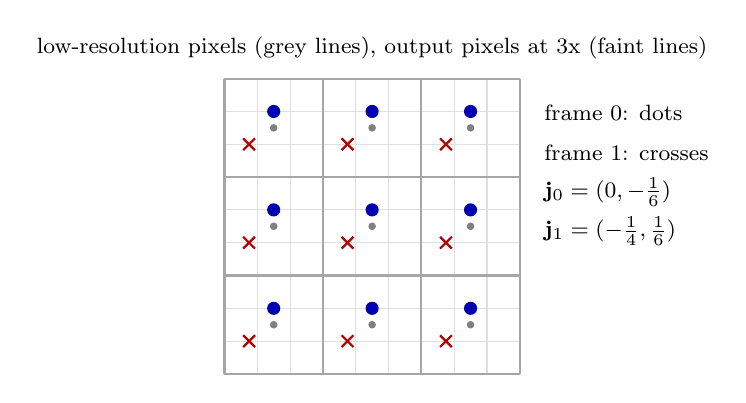
\begin{tikzpicture}[scale=1.25]
  \foreach \k in {0,...,9}{
    \draw[gray!25] (\k/3,-3) -- (\k/3,0);
    \draw[gray!25] (0,-\k/3) -- (3,-\k/3);
  }
  \draw[gray!70, thick] (0,-3) grid (3,0);
  \foreach \i in {0,1,2}{
    \foreach \j in {0,1,2}{
      \fill[gray] (\i+0.5,-\j-0.5) circle (1.1pt);
      \fill[blue!70!black] (\i+0.5,-\j-0.5+0.1667) circle (1.9pt);
      \draw[red!70!black, thick] (\i+0.25-0.06,-\j-0.6667-0.06) -- (\i+0.25+0.06,-\j-0.6667+0.06);
      \draw[red!70!black, thick] (\i+0.25-0.06,-\j-0.6667+0.06) -- (\i+0.25+0.06,-\j-0.6667-0.06);
    }
  }
  \node[anchor=south, font=\footnotesize] at (1.5,0.1) {low-resolution pixels (grey lines), output pixels at 3x (faint lines)};
  \node[anchor=west, font=\footnotesize] at (3.15,-0.35) {frame $0$: dots};
  \node[anchor=west, font=\footnotesize] at (3.15,-0.75) {frame $1$: crosses};
  \node[anchor=west, font=\footnotesize] at (3.15,-1.15) {$\mathbf j_0=(0,-\tfrac16)$};
  \node[anchor=west, font=\footnotesize] at (3.15,-1.55) {$\mathbf j_1=(-\tfrac14,\tfrac16)$};
\end{tikzpicture}
\caption{Sample positions of two consecutive frames inside a $3\times3$ patch of low-resolution pixels, with rows increasing downwards as in the code. Grey dots mark the pixel centres. Blue dots are the samples of frame $0$ and red crosses those of frame $1$, shifted by the first two Halton offsets of \cref{tab:bg-halton}. Faint lines mark the output pixels at 3x, which at this scale subdivide each low-resolution pixel into nine cells.}\label{fig:bg-jitter}
\end{figure}

\paragraph{Halton sequence.} The offsets come from the Halton $(2,3)$ sequence, a low-discrepancy sequence whose points spread evenly over the unit square with fewer large gaps than random points.\cite{halton1960efficiency} For an integer $n\ge1$ with base-$b$ digits $n=\sum_k d_k(n)\,b^k$, the radical inverse is
\begin{equation}
\varphi_b(n)=\sum_{k\ge0}d_k(n)\,b^{-(k+1)}.\label{eq:bg-halton}
\end{equation}
For example, $3=11_2$ gives $\varphi_2(3)=\tfrac12+\tfrac14=\tfrac34$, and $3=10_3$ gives $\varphi_3(3)=\tfrac19$. The function \texttt{halton} computes this by repeated division by the base. Frame $t$ uses the index $n_t=(t\bmod16)+1$ and the offset
\begin{equation}
\mathbf j_t=\big(\varphi_2(n_t)-\tfrac12,\ \varphi_3(n_t)-\tfrac12\big),\label{eq:bg-jitter}
\end{equation}
so the sequence repeats every 16 frames. The index starts at 1 because index 0 would give the corner $(-0.5,-0.5)$. Training gives each sample a random starting point in the cycle. \Cref{tab:bg-halton} lists the first four offsets, which \texttt{jitter\_sequence} produces.

\begin{table}[!htbp]
\caption{First four Halton jitter offsets. Frame $t$ uses index $n=(t\bmod16)+1$, and the offset $\mathbf j_t$ of Eq.~(\ref{eq:bg-jitter}) is in low-resolution pixels. The values were printed by \texttt{jitter\_sequence} and are rounded to three decimals}\label{tab:bg-halton}
\begin{tabular*}{\columnwidth}{@{\extracolsep\fill}rrrrrr}
\toprule
Frame $t$ & $n$ & $\varphi_2(n)$ & $\varphi_3(n)$ & $j_x$ & $j_y$ \\
\midrule
0 & 1 & $0.500$ & $0.333$ & $0.000$ & $-0.167$ \\
1 & 2 & $0.250$ & $0.667$ & $-0.250$ & $0.167$ \\
2 & 3 & $0.750$ & $0.111$ & $0.250$ & $-0.389$ \\
3 & 4 & $0.125$ & $0.444$ & $-0.375$ & $-0.056$ \\
\botrule
\end{tabular*}
\end{table}

\paragraph{Why jitter and accumulation recover resolution.} Take a static scene and one jittered sample per low-resolution pixel per frame. If the samples of earlier frames are placed at their true positions, using each frame's known offset, then after $N$ frames each low-resolution pixel holds $N$ samples at $N$ different positions. The output needs $s^2$ pixels per low-resolution pixel, so the samples must cover the $s^2$ sub-cells, and the Halton positions do this within a few frames. Jitter-aware upsampling does the placement: it samples the low-resolution frame at the output pixel centre minus the jitter (\texttt{jitter\_upsample}), so each sample lands at its true position.

Accumulation is a weighted average. Consider an exponential average $\hat y=\sum_{k\ge0}w_kx_{t-k}$ with weights $w_k=\alpha(1-\alpha)^k$, $0<\alpha\le1$, which sum to one. For samples $x_{t-k}$ with independent noise of variance $\sigma^2$,
\begin{equation}
\operatorname{Var}\hat y=\sum_{k\ge0}w_k^2\sigma^2=\frac{\alpha^2\sigma^2}{1-(1-\alpha)^2}=\frac{\alpha}{2-\alpha}\,\sigma^2,
\end{equation}
so the average behaves like a mean of $N_{\text{eff}}=(2-\alpha)/\alpha$ independent samples. For $\alpha=0.1$, the blend used by the analytic baseline of \cref{sec:bg-taa}, $N_{\text{eff}}=19$. This holds only when the history is aligned, so that a sample from an earlier frame belongs to the same surface point, and when the content is static. Motion and disocclusion break both conditions, which is why the next subsections need reprojection and rejection.

\subsection{Motion vectors and optical flow}\label{sec:bg-motion}

\paragraph{Flow.} For frames $t$ and $s$, the flow $F_{t\to s}$ is a field of displacements in pixels. For a pixel $\mathbf p$ of frame $t$, the point $\mathbf p+F_{t\to s}(\mathbf p)$ is the position in frame $s$ of the surface point that $\mathbf p$ shows in frame $t$. The code uses the backward convention for warping, in which the field is defined on the grid of the frame being produced, $t$, and points into the source frame $s$. Frame $t$ is then predicted from frame $s$ by
\begin{equation}
\hat I_t(\mathbf p)=I_s\big(\mathbf p+F_{t\to s}(\mathbf p)\big),\label{eq:bg-flow}
\end{equation}
which is the backward warp of \cref{sec:bg-warp}. A forward flow $F_{s\to t}$ is defined on the grid of the source frame and points forward. Datasets often store forward flow, and warping with it needs a scatter step that leaves holes and overlaps, so the code converts or reverses the flow instead. The code uses these conventions:
\begin{itemize}
\item Temporal super-resolution: the motion vector of frame $t$ is $m_t=F_{t\to t-1}$, the displacement from the current frame to the previous one, at low-resolution pixels (\texttt{sr\_batch}, \texttt{raft\_mv\_and\_valid}).
\item Frame generation: the engine motion vector of the newest real frame is $M_1=F_{1\to0}$, the displacement from $I_1$ to $I_0$ (\texttt{fg\_batch}).
\item Frame generation: the intermediate flows are $F_{\tau\to0}$ and $F_{\tau\to1}$, the outputs of \texttt{IFNet} (\cref{sec:bg-interp}).
\item Exact sources: the loader plays clips with forward flow backwards (\texttt{load\_clip}). The stored flow from frame $i$ to frame $i+1$ then becomes the displacement from the later frame to the earlier one, which is the convention of $m_t$, without any inversion.
\end{itemize}

\paragraph{Engine vectors and colour flow.} An engine writes a motion vector per pixel from the transforms of the geometry it draws. The vector is exact for opaque surfaces that the engine transforms, and particles and other effects without a transform get none, which is why engines also write a reactive mask. Research systems use such engine buffers, including motion vectors, as network inputs.\cite{xiao2020nsrr} Colour-only flow estimates motion from the images. It works on any video, but it is an estimate that can be wrong at boundaries, and it cannot separate motion from a change of lighting or from an overlay that moves independently. The code uses torchvision's RAFT-Small \cite{teed2020raft} with 12 updates (\texttt{load\_raft}, \texttt{raft\_flow}), as the teacher for motion labels on real video and for tOF. The built-in motion estimator of the temporal super-resolution network is an IFNet \cite{huang2022rife}.

\paragraph{Forward-backward consistency.} For two frames $a$ and $b$ with flows $F_{a\to b}$ and $F_{b\to a}$, a pixel passes the round-trip test when
\begin{equation}
\big\|F_{a\to b}(\mathbf p)+F_{b\to a}\big(\mathbf p+F_{a\to b}(\mathbf p)\big)\big\|<1+0.05\,\big\|F_{a\to b}(\mathbf p)\big\|,\label{eq:bg-fb}
\end{equation}
which says that going to frame $b$ and back returns to the start within one pixel plus 5 percent of the flow. The code's \texttt{raft\_mv\_and\_valid} applies this test with $a$ the current frame and marks the pixels that pass as valid. Pixels that fail lie at occlusions, at disocclusions and where the flow estimate is poor.

\paragraph{Occlusion and disocclusion.} A surface point is disoccluded in frame $t$ when it is visible in $t$ but absent from the previous frame $s$, and it is occluded when it is visible in $s$ but covered in $t$. The warp of Eq.~(\ref{eq:bg-flow}) has no correct source for a disoccluded pixel, so history must not be used there. The code's validity mask $v$ equals 1 where the pixel of frame $t$ is visible in the previous frame, so $1-v$ marks the disoccluded pixels (\texttt{load\_valid}). The temporal super-resolution network also uses a depth cue, $|d_t-\mathcal W(d_{t-1})|/(|d_t|+10^{-3})$, clipped to $[0,1]$, as an input feature (\texttt{TSRNet.forward}).

\paragraph{Scene cuts.} A cut is a change of content between consecutive frames. No point corresponds across it, so any flow is meaningless, and no frame can be predicted from the one before. The code detects cuts with the distance between normalised 32-bin histograms of the luma (\texttt{cut\_score}),
\begin{equation}
d_{\text{hist}}(I_0,I_1)=\tfrac12\sum_{b=1}^{32}\big|h_0(b)-h_1(b)\big|,\label{eq:bg-cut}
\end{equation}
where $h_0$ and $h_1$ are the normalised histograms of the two frames. This distance lies in $[0,1]$ and is the total-variation distance between the two histograms. When the motion vector $M_1$ is available, the score adds $2\,\overline{|I_1-\mathcal W(I_0,M_1)|}$, twice the mean motion-compensated difference. A score above a threshold is a cut.

\subsection{Warping, reprojection and history accumulation}\label{sec:bg-warp}

\paragraph{Backward warping.} Given a frame $I$ and a flow $F$, the warp $\mathcal W(I,F)(\mathbf p)=I(\mathbf p+F(\mathbf p))$ must be evaluated at non-integer positions. The code uses bilinear interpolation. For $\mathbf q=\mathbf p+F(\mathbf p)$ with integer part $(x_0,y_0)$ and fractional parts $a=q_x-x_0$ and $b=q_y-y_0$,
\begin{equation}\begin{split}
I(\mathbf q)&=(1-a)(1-b)\,I(x_0,y_0)+a(1-b)\,I(x_0+1,y_0)\\
&\quad+(1-a)b\,I(x_0,y_0+1)+ab\,I(x_0+1,y_0+1).
\end{split}\label{eq:bg-warp}\end{equation}
The four weights are non-negative and sum to one. Positions outside the frame are clamped to the border. Backward warping gathers each output pixel from one source location, so the output has no holes or overlaps, which forward splatting cannot guarantee. \texttt{backward\_warp} implements Eq.~(\ref{eq:bg-warp}) with \texttt{grid\_sample}, using the coordinate mapping of RIFE, in which pixel index $i$ corresponds to the normalised coordinate $-1+2i/(W-1)$. \Cref{fig:bg-warp} shows one pixel.

\begin{figure}[!htbp]
\centering
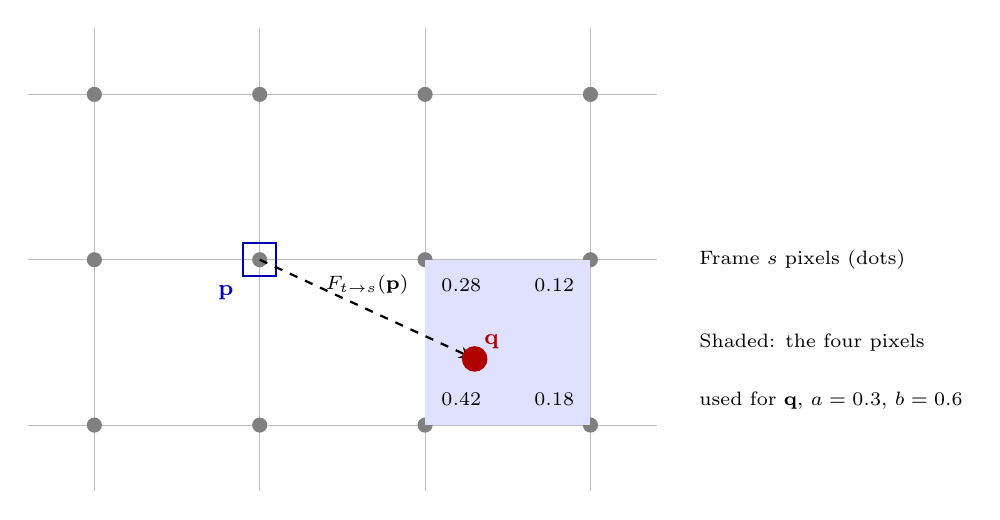
\begin{tikzpicture}[scale=2.1, font=\footnotesize]
  \draw[gray!50] (-0.4,-2.4) grid (3.4,0.4);
  \foreach \i in {0,...,3}{\foreach \j in {0,...,2}{\fill[gray] (\i,-\j) circle (1.3pt);}}
  \fill[blue!12] (2,-2) rectangle (3,-1);
  \draw[blue!70!black, thick] (0.9,-0.9) rectangle (1.1,-1.1);
  \node[anchor=north east, text=blue!70!black] at (0.9,-1.1) {$\mathbf p$};
  \draw[-{Stealth[length=2mm]}, thick, dashed] (1,-1) -- (2.3,-1.6);
  \node[anchor=south, font=\scriptsize] at (1.65,-1.27) {$F_{t\to s}(\mathbf p)$};
  \fill[red!70!black] (2.3,-1.6) circle (2.2pt);
  \node[anchor=south west, text=red!70!black] at (2.3,-1.6) {$\mathbf q$};
  \node[anchor=north west] at (2.04,-1.06) {\scriptsize $0.28$};
  \node[anchor=north east] at (2.96,-1.06) {\scriptsize $0.12$};
  \node[anchor=south west] at (2.04,-1.94) {\scriptsize $0.42$};
  \node[anchor=south east] at (2.96,-1.94) {\scriptsize $0.18$};
  \node[anchor=west] at (3.6,-1.0) {\scriptsize Frame $s$ pixels (dots)};
  \node[anchor=west] at (3.6,-1.5) {\scriptsize Shaded: the four pixels};
  \node[anchor=west] at (3.6,-1.85) {\scriptsize used for $\mathbf q$, $a=0.3$, $b=0.6$};
\end{tikzpicture}
\caption{Backward warp of one pixel. Pixel $\mathbf p=(1,1)$ of frame $t$ takes the value at $\mathbf q=\mathbf p+F_{t\to s}(\mathbf p)=(2.3,1.6)$ in frame $s$. That value is the bilinear mixture of the four surrounding pixels of frame $s$, with the weights shown from Eq.~(\ref{eq:bg-warp}). The flow is illustrative.}\label{fig:bg-warp}
\end{figure}

\paragraph{Half-pixel attenuation.} Bilinear interpolation is a low-pass filter. For a shift of half a pixel the weights are $(\tfrac12,\tfrac12)$, and the frequency response at angular frequency $\omega$ radians per pixel is $\tfrac12(1+e^{-i\omega})$, whose magnitude is $|\cos(\omega/2)|$. At $\omega=\pi/2$ this is $\cos(\pi/4)\approx0.71$, and at the Nyquist frequency $\omega=\pi$ it is zero. Each warp at a fractional offset removes part of the high-frequency content. A recurrent network that warps its output every frame loses high frequencies at every step unless its residual path adds them back.

\paragraph{Reprojection and accumulation.} Reprojection moves a stored result to the current frame. A history image $H$ from frame $t-1$ becomes $H_t(\mathbf p)=\mathcal W(H,m_t)(\mathbf p)$ with $m_t=F_{t\to t-1}$, and accumulation then combines $H_t$ with the new samples. The recurrent state of the temporal super-resolution network, its output and its hidden feature map, is reprojected in the same way with the low-resolution vectors. A pixel whose motion is wrong, or which is disoccluded, takes its history from the wrong surface, and that is the source of the ghosting described in \cref{sec:bg-taa}.

\subsection{Temporal anti-aliasing and temporal upscaling}\label{sec:bg-taa}

Temporal anti-aliasing (TAA) \cite{yang2020taasurvey} combines jittered samples over time with a history buffer. For each frame it renders with a jittered sample grid, reprojects the history with motion vectors, clamps the reprojected history to the range of the current samples in a small neighbourhood, and blends the clamped history with the current samples. Temporal upscaling runs the same loop at a lower render resolution, with the accumulation buffer at output resolution.

\paragraph{Exponential blending.} Without reprojection and clamping, accumulation is $\hat y_t=\alpha x_t+(1-\alpha)\hat y_{t-1}$, where $x_t$ is the current sample value and $0<\alpha\le1$. Unrolling gives
\begin{equation}
\hat y_t=\sum_{k=0}^{t-1}\alpha(1-\alpha)^k\,x_{t-k}+(1-\alpha)^t\,\hat y_0,\label{eq:bg-ema-unroll}
\end{equation}
so the sample $k$ frames old has weight $\alpha(1-\alpha)^k$, and the initial value keeps the weight $(1-\alpha)^t$. \Cref{fig:bg-ema} shows these weights for $\alpha=0.1$. A sample 10 frames old has weight $0.035$, and the initial value still has weight $0.12$ after 20 frames.

\begin{figure}[!htbp]
\centering
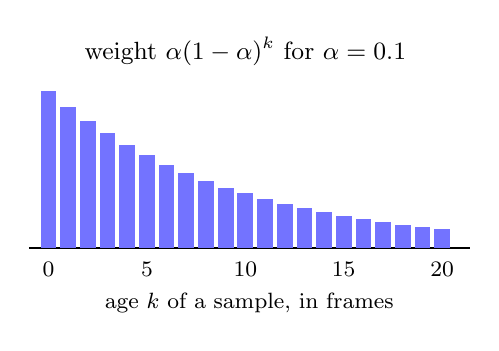
\begin{tikzpicture}[x=0.5cm, font=\footnotesize]
  \draw[thick] (-0.3,0) -- (10.9,0);
  \foreach \k/\h in {0/2.00,1/1.80,2/1.62,3/1.46,4/1.31,5/1.18,6/1.06,7/0.96,8/0.86,9/0.77,10/0.70,11/0.63,12/0.56,13/0.51,14/0.46,15/0.41,16/0.37,17/0.33,18/0.30,19/0.27,20/0.24}{
    \fill[blue!55] (\k*0.5,0) rectangle (\k*0.5+0.4,\h);
  }
  \foreach \k in {0,5,10,15,20}{
    \node[below] at (\k*0.5+0.2,-0.05) {\k};
  }
  \node[below] at (5.3,-0.45) {age $k$ of a sample, in frames};
  \node[above] at (5.2,2.2) {\small weight $\alpha(1-\alpha)^k$ for $\alpha=0.1$};
\end{tikzpicture}
\caption{Weight of a sample $k$ frames old in the exponential average of \cref{eq:bg-ema-unroll} with $\alpha=0.1$. The bar height is the weight times 20, in centimetres of the drawing. The weights fall geometrically, so an old surface that stays in the history fades slowly, which is the ghosting trail that clamping limits.}\label{fig:bg-ema}
\end{figure}

\paragraph{Ghosting.} When a surface changes, because it is disoccluded, because its motion vector is wrong or because an object leaves a region, the history still holds the old surface. That surface keeps the weight $(1-\alpha)^k$ for $k$ frames and appears as a trail behind moving objects. Clamping limits the trail. The reprojected value is confined to the range of the current neighbourhood, so an old colour far from the new samples is pulled back to the range boundary. Ghosting remains when the old colour lies inside that range, which happens when a surface and its background have similar colours. A larger $\alpha$ reduces ghosting but also reduces the averaging that removes aliasing, and that trade-off is the central design choice of TAA.

\paragraph{Analytic baseline.} The analytic upscaler of the evaluation (\texttt{AnalyticTAAU} in \texttt{nss\_metrics.py}, run by \texttt{run\_taau} in \texttt{nss\_eval.py}) implements the loop with fixed rules and stands in for analytic TAA upscalers without their proprietary heuristics. For frame $t$, with low-resolution colour $x_t$, jitter $\mathbf j_t$ and low-resolution motion vector $m_t$, it performs the following steps.
\begin{enumerate}
\item Base image: $B_t(\mathbf p)$ is the bilinear interpolation of $x_t$ at the low-resolution position of the output pixel centre $\mathbf p$ minus $\mathbf j_t$, so each sample is placed at its true position.
\item If there is no history, the output is $B_t$.
\item History: $H_t=\mathcal W\big(\hat y_{t-1},\,s\,U(m_t)\big)$, where $U$ is bilinear upsampling by $s$ and the factor $s$ converts low-resolution displacements into output pixels.
\item Clamp: with $lo$ and $hi$ the channel-wise minimum and maximum of YCoCg$(B_t)$ over the $3\times3$ output neighbourhood of each pixel, the history is clamped in YCoCg to the box between $lo$ and $hi$, and $H'_t$ is the RGB value of the clamped history.
\item Blend: $\hat y_t=H'_t+0.1\,(B_t-H'_t)$, which is 90 percent history and 10 percent current base image.
\end{enumerate}
The displayed output is clamped to $[0,1]$, but the unclamped value becomes the next history. Step 5 gives
\begin{equation}
\hat y_t=0.9\,H'_t+0.1\,B_t.\label{eq:bg-taa}
\end{equation}

Two properties of this baseline matter for the comparison. First, its docstring says that it resets on invalid history, but the code has no validity test, so every frame reprojects and clamps the history and no disocclusion rejection takes place. Second, the motion vectors are sampled at the jittered sample positions (\texttt{\_sr\_inputs}), while the baseline interprets low-resolution vectors as if they were at the pixel centres. The resulting error is the jitter times the local gradient of the motion field, which vanishes for uniform motion and is largest at motion boundaries. The temporal super-resolution network receives the same low-resolution vectors and interprets them in the same way. The supplement describes these properties as they are in the code.

\subsection{Neural building blocks}\label{sec:bg-cnn}

The networks use a small set of operators. Each is defined here with the code's convention and with the reason for its use.

\paragraph{Convolution and multiply-accumulates.} A convolutional layer with $C_{\text{in}}$ input channels, $C_{\text{out}}$ output channels and a $k\times k$ kernel $K$ computes, with stride 1 and padding $(k-1)/2$,
\begin{equation}
Y[o,i,j]=b_o+\sum_{c=1}^{C_{\text{in}}}\sum_{u=0}^{k-1}\sum_{v=0}^{k-1}K[o,c,u,v]\;X\!\Big[c,\;i+u-\tfrac{k-1}{2},\;j+v-\tfrac{k-1}{2}\Big],\label{eq:bg-conv}
\end{equation}
where $X$ is the input, $Y$ the output and $b_o$ the bias of output channel $o$. The sum is a cross-correlation, which is PyTorch's convention. One multiply-accumulate (MAC) is one multiplication followed by one addition. Each output element of Eq.~(\ref{eq:bg-conv}) costs $C_{\text{in}}k^2$ MACs, so a layer with an $H\times W$ output costs
\begin{equation}
M=H\,W\,C_{\text{out}}\,C_{\text{in}}\,k^2\qquad\text{MACs},\label{eq:bg-macs}
\end{equation}
and grouped convolutions divide this by the number of groups. A transposed convolution from an $H_{\text{in}}\times W_{\text{in}}$ input costs $H_{\text{in}}W_{\text{in}}C_{\text{in}}C_{\text{out}}k^2$, because each input pixel scatters a $k\times k$ kernel into every output channel. Pixel shuffles, bilinear resizing and grid sampling perform no such multiply-accumulates in the count, so the warps are excluded from the cost figures, as in \cref{M-tab:tiers}. For example, a $3\times3$ convolution with 24 input and 24 output channels costs $24\cdot24\cdot9=5{,}184$ MACs per output pixel.

\paragraph{Cost per 1080p frame.} The code counts MACs with forward hooks (\texttt{count\_macs}) on the fused network, which is the deployed form in which every block is a plain convolution. For temporal super-resolution it runs one step with a history state on a $64\times64$ low-resolution input, including the built-in motion estimator, and divides the count by $64^2$ to obtain MACs per low-resolution pixel (\texttt{tsr\_macs\_per\_lr\_pixel}). Each layer's cost is proportional to its pixel count, so the cost of one output frame is that per-pixel count times the number of low-resolution pixels of the 1080p output,
\begin{equation}
G_{1080p}=\frac{M_{\text{pix}}\,(1920/s)(1080/s)}{10^{9}}\quad\text{GMAC}.\label{eq:bg-gmac}
\end{equation}
For frame generation the fused network runs on a $272\times480$ frame. The flow-resolution limit is scaled by $272/1080$ so that the flow runs at the scale that a 1080p frame would use, the MACs are counted, and the count is multiplied by $(1920\cdot1080)/(272\cdot480)$. This assumes that the cost is linear in the pixel count, which holds for convolutions and is approximate for the remaining operators. A MAC count is a cost measure and not a time, and the latency measurements are reported separately.

\paragraph{Pixel shuffle.} Pixel shuffle \cite{shi2016espcn} rearranges a tensor with $C r^2$ channels at $H\times W$ into $C$ channels at $rH\times rW$,
\begin{equation}
Z[c,\;rh+a,\;rw+b]=X[c\,r^2+a\,r+b,\;h,\;w],\qquad 0\le a,b<r,\label{eq:bg-shuffle}
\end{equation}
without any multiplication. Its inverse, pixel unshuffle or space-to-depth, folds a tensor at $rH\times rW$ into $r^2$ times as many channels at $H\times W$. A convolution can therefore run at low resolution, where it is cheap, and the shuffle restores the output size. The temporal super-resolution network uses both directions. Its output convolution produces $4s^2$ channels at low resolution, which the shuffle turns into a residual and a history weight at output resolution, and it folds the reprojected output into $3s^2$ low-resolution channels before the trunk reads it.

\paragraph{Structural re-parameterisation.} A block can be trained as several parallel linear branches and deployed as one convolution. This works when the branches share their input and their spatial support, because convolution is linear in its kernel. The RepConv block of \texttt{nss\_models.py} has four branches on the same input $x$, with $C_{\text{in}}$ input and $C_{\text{out}}$ output channels:
\begin{enumerate}
\item a $3\times3$ convolution with kernel $W_3$ and bias $b_3$.
\item a $1\times1$ convolution with kernel $W_1$ and bias $b_1$.
\item the identity, present when $C_{\text{in}}=C_{\text{out}}$.
\item fixed edge filters $E_1$ (Sobel $x$), $E_2$ (Sobel $y$) and $E_3$ (Laplacian), applied to every input channel, whose $3C_{\text{in}}$ responses are combined by a learned $1\times1$ projection $P\in\mathbb R^{C_{\text{out}}\times3C_{\text{in}}}$ with bias $b_e$.
\end{enumerate}
The block output is $\phi(Y)$, where $\phi$ is a PReLU activation and $Y$ is the sum of the four branch outputs.

The four branches fold into one $3\times3$ convolution, exactly:
\begin{equation}\begin{split}
Y&=\sum_{c}K[\cdot,c]\ast x_c+b,\\
K[o,c]&=W_3[o,c]+\operatorname{pad}\big(W_1[o,c]\big)\\
&\quad+\sum_{k=1}^{3}\tilde P[o,c,k]\,E_k+\delta_{oc}\,\Delta,\\
b&=b_3+b_1+b_e,
\end{split}\label{eq:bg-fold}\end{equation}
where $\ast$ is convolution with stride 1 and padding 1, $\operatorname{pad}$ places a scalar at the centre tap of an otherwise zero $3\times3$ kernel, $\tilde P[o,c,k]=P[o,\,3c+k]$ reorders the projection by input channel, $\delta_{oc}$ is the Kronecker delta and $\Delta$ is the $3\times3$ kernel with 1 at its centre and 0 elsewhere.

\emph{Proof.} Each branch is linear in $x$ and is a convolution with stride 1 and padding 1, so each can be written as a $3\times3$ convolution. (1) The $1\times1$ branch outputs $W_1[o,c]\,x_c(\mathbf p)$. With padding 1, a $3\times3$ kernel whose only nonzero tap is the centre, with value $W_1[o,c]$, produces the same output, and that kernel is $\operatorname{pad}(W_1[o,c])$. (2) The identity outputs $x_o(\mathbf p)$, which is the kernel $\Delta$ on the diagonal $c=o$. (3) The edge branch outputs $\sum_c\sum_k P[o,3c+k]\,(E_k\ast x_c)(\mathbf p)+b_e[o]$. Convolution is linear in its kernel, so $\sum_k\tilde P[o,c,k]\,(E_k\ast x_c)=\big(\sum_k\tilde P[o,c,k]E_k\big)\ast x_c$, and the branch is a $3\times3$ convolution with kernel $\sum_k\tilde P[o,c,k]E_k$ and bias $b_e[o]$. (4) For a common stride and padding, $(A\ast x)+(B\ast x)=(A+B)\ast x$, so the four branch sums combine into Eq.~(\ref{eq:bg-fold}). The activation is applied after the sum, so it is not folded, and the fold is exact. Up to floating-point rounding, the fused and unfused outputs are identical, and the code's fusion-parity test checks this numerically. $\square$

Training uses the folded kernel directly. The code recomputes $K$ from the branch parameters on every forward pass (online re-parameterisation), so a block costs one $3\times3$ convolution during training as well as in deployment. The function class is unchanged, because $W_3$ alone can represent any kernel that the block can reach. The extra branches only change which kernels gradient descent reaches. The $1\times1$ and edge-projection weights start at zero, so the block starts as a $3\times3$ convolution plus the identity. Only the weights are zeroed, so the small biases $b_1$ and $b_e$ remain at their random initial values. \Cref{fig:bg-fold} summarises the fold.

\begin{figure}[!htbp]
\centering
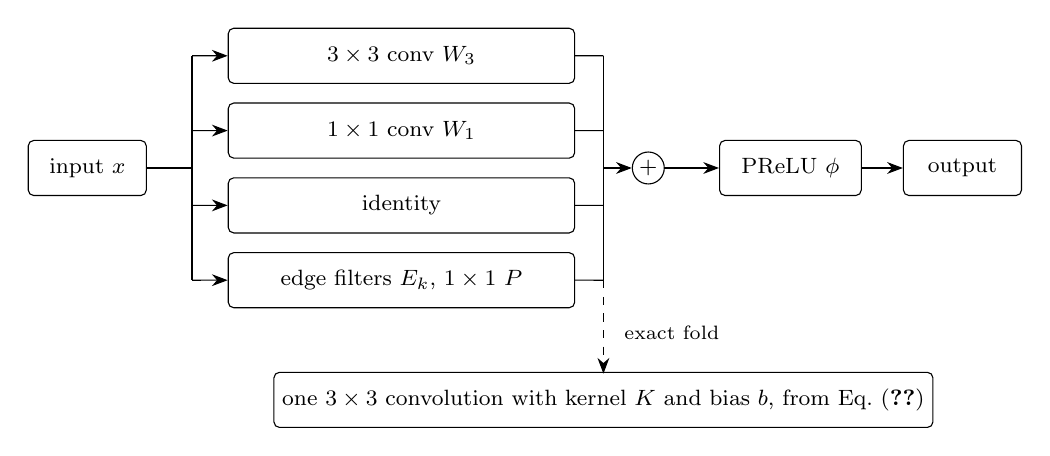
\begin{tikzpicture}[scale=0.95, font=\footnotesize, node distance=3mm,
  box/.style={draw, rounded corners=2pt, align=center, minimum height=7mm, minimum width=4.4cm, inner sep=3pt},
  arr/.style={-{Stealth[length=2mm]}}]
\node[box, minimum width=1.5cm] (x) at (0,0) {input $x$};
\node[box] (w3) at (4.2,1.5) {$3\times3$ conv $W_3$};
\node[box] (w1) at (4.2,0.5) {$1\times1$ conv $W_1$};
\node[box] (id) at (4.2,-0.5) {identity};
\node[box] (ed) at (4.2,-1.5) {edge filters $E_k$, $1\times1$ $P$};
\node[draw, circle, inner sep=1pt] (sum) at (7.5,0) {$+$};
\node[box, minimum width=1.8cm] (act) at (9.4,0) {PReLU $\phi$};
\node[box, minimum width=1.5cm] (out) at (11.7,0) {output};
\draw (x.east) -- (1.4,0);
\draw (1.4,1.5) -- (1.4,-1.5);
\draw[arr] (1.4,1.5) -- (w3.west);
\draw[arr] (1.4,0.5) -- (w1.west);
\draw[arr] (1.4,-0.5) -- (id.west);
\draw[arr] (1.4,-1.5) -- (ed.west);
\draw (w3.east) -- (6.9,1.5);
\draw (w1.east) -- (6.9,0.5);
\draw (id.east) -- (6.9,-0.5);
\draw (ed.east) -- (6.9,-1.5);
\draw (6.9,1.5) -- (6.9,-1.5);
\draw[arr] (6.9,0) -- (sum.west);
\draw[arr] (sum.east) -- (act.west);
\draw[arr] (act.east) -- (out.west);
\node[box, minimum width=7.0cm] (k) at (6.9,-3.1) {one $3\times3$ convolution with kernel $K$ and bias $b$, from Eq.~(\ref{eq:bg-fold})};
\draw[arr, dashed] (6.9,-1.5) -- (6.9,-2.75);
\node[anchor=west, font=\scriptsize] at (7.05,-2.2) {exact fold};
\end{tikzpicture}
\caption{Re-parameterisation of one RepConv block. The four linear branches share the input and sum before the activation, giving one kernel $K$ and bias $b$ of size $3\times3$.}\label{fig:bg-fold}
\end{figure}

\paragraph{U-Net levels.} The trunk of the temporal super-resolution network has an optional half-resolution level. It differs from the classic U-Net,\cite{ronneberger2015unet} so it is described precisely here. A strided $3\times3$ convolution halves the resolution and doubles the channels. Residual blocks run at half resolution, a $1\times1$ convolution doubles the channels to $4w$, and a pixel shuffle returns to full resolution with $w$ channels. The result is added to the features that entered the level, which is an additive skip, where the classic U-Net concatenates. A convolution with $2w$ channels at half resolution costs the same as one with $w$ channels at full resolution, because $(2w)^2\cdot\tfrac14=w^2$, but each of its taps covers twice the distance in the original image.

\paragraph{Recurrent networks and hidden-state warping.} A recurrent network carries a state from frame to frame. The state of the temporal super-resolution network holds the previous output $\hat y_{t-1}$, a hidden feature map $h_{t-1}$, and the previous depth, colour and jitter. At each frame the network reads the current inputs together with the reprojected output and hidden state, and writes the new output and a new hidden state $h_t=\tanh(\cdot)$ of a convolution. The hidden state is reprojected with the same motion as the output, $\mathcal W(h_{t-1},m_t)$, because its channels describe the content at each pixel, and a feature warped with the wrong motion describes a different surface. Training unrolls the network over several frames, with a 16-frame unroll every fourth step, and backpropagates through the whole unroll, which is backpropagation through time. During the first quarter of training (\texttt{mv\_warmup\_frac} $=0.25$), samples without motion vectors warp the history with the label motion instead of the estimated motion. The probability of doing so falls linearly from one to zero over that quarter. Feeding the label in place of the model's own estimate is teacher forcing, which this code applies as a schedule, and the schedule stops the history path from learning to ignore history while the estimator is still poor.

\paragraph{Zero initialisation.} A branch whose output layer has zero weights and a zero bias contributes exactly zero at initialisation, so the network starts as the network without that branch. Two consequences follow. The output layer receives a nonzero gradient, because its input features are nonzero, so it learns from the first step. The layers upstream of it receive a zero gradient at the first step, because they reach the loss only through the zero weights, and they start to learn once the output layer is nonzero. The bias must also be zero, because a nonzero bias gives a constant contribution at initialisation. The code uses three instances.
\begin{itemize}
\item The engine-hint input channels of the first convolution in each IFNet block have zero weights, so the hints do not change that layer's output at initialisation. This is exact.
\item The frame generator's residual head has zero weights and a zero bias, so its colour residual $r$ is zero at initialisation. Its UI logit has a bias of $-4$, so the UI weight is $u=\sigma(-4)\approx0.018$ at initialisation. The output is therefore $u\,I_1+(1-u)$ times the RIFE blend $m\mathcal W(I_0,F_{\tau\to0})+(1-m)\mathcal W(I_1,F_{\tau\to1})$, and differs from that blend by $u\,(I_1-\text{blend})$. The code's parity test compares the blend, not the final output, so a fresh model reproduces the blend of RIFE exactly and not its final output.
\item The temporal super-resolution output layer has zero weights and a zero bias, so the residual is zero and the history weight is $\sigma(0+2)\approx0.88$, since the code adds 2 to the logit before the sigmoid. At initialisation the output is therefore $0.88$ of the history and $0.12$ of the jitter-aware upsampling, an exponential blend of the kind described in \cref{sec:bg-taa}.
\end{itemize}

\paragraph{Mixed precision and loss scaling.} In IEEE half precision (FP16) a value has one sign bit, five exponent bits and ten fraction bits. Its largest finite value is $(2-2^{-10})\,2^{15}=65{,}504$, its smallest positive normal value is $2^{-14}\approx6.1\cdot10^{-5}$, and its smallest positive subnormal value is $2^{-24}\approx6.0\cdot10^{-8}$. Two failures follow. Activations above 65{,}504 become infinite, and gradients much smaller than $6\cdot10^{-8}$ round to zero. Mixed precision \cite{micikevicius2018mixed} runs the forward and backward passes in FP16 and keeps FP32 copies of the weights. Loss scaling multiplies the loss by a scale $S$ before the backward pass, so that small gradients stay representable, and divides the gradients by $S$ before the optimiser step. Dynamic loss scaling lowers $S$ when a step produces non-finite gradients and raises it again after a run of finite steps. The code uses PyTorch's \texttt{GradScaler} with autocast. It scales the loss, unscales the gradients, clips their norm to 1.0 (\texttt{grad\_clip}) and then steps the optimiser. A run stops when the loss stays non-finite for 200 steps by default.

\paragraph{Exponential moving average.} The optimiser updates the weights $w_k$, and the code also keeps the average
\begin{equation}
\bar w_k=d_k\,\bar w_{k-1}+(1-d_k)\,w_k,\qquad d_k=\min\!\Big(0.999,\ \frac{1+k}{10+k}\Big),\label{eq:bg-ema}
\end{equation}
which is used for validation and checkpoints, while the raw weights produce the gradients. The warm-up in $d_k$ means that the decay reaches 0.999 only after about 9{,}000 steps, so early in training the average follows the weights closely. At a decay of 0.999 the average has a memory of about $1/(1-0.999)=1{,}000$ steps.

\paragraph{AdamW.} AdamW \cite{loshchilov2019adamw} keeps running averages of the gradient and of its square, $m_k=\beta_1 m_{k-1}+(1-\beta_1)g_k$ and $v_k=\beta_2 v_{k-1}+(1-\beta_2)g_k^2$, corrects their start-up bias and applies
\begin{equation}
\theta_k=\theta_{k-1}-\eta\Big(\frac{\hat m_k}{\sqrt{\hat v_k}+\epsilon}+\lambda\,\theta_{k-1}\Big),\qquad \hat m_k=\frac{m_k}{1-\beta_1^k},\quad \hat v_k=\frac{v_k}{1-\beta_2^k},\label{eq:bg-adamw}
\end{equation}
where $g_k$ is the gradient, $\eta$ the learning rate and $\lambda$ the weight decay. The decay term $\lambda\theta$ acts on the weights directly and is not added to the gradient, which is the difference from Adam with an L2 penalty. The code uses $(\beta_1,\beta_2)=(0.9,0.99)$, PyTorch's default $\epsilon=10^{-8}$ and $\lambda=10^{-4}$.

\paragraph{Learning-rate schedule.} The schedule is driven by wall-clock time rather than by the step count. With progress $p\in[0,1]$, the elapsed fraction of the run's time budget, a warm-up fraction $w=0.03$, a peak rate $\eta_0$ and a floor $\eta_{\min}=10^{-6}$,
\begin{equation}
\eta(p)=\begin{cases}\eta_0\,\max(p/w,\,0.01), & p<w,\\[2pt] \eta_{\min}+\tfrac12(\eta_0-\eta_{\min})\big(1+\cos\pi\tau\big), & \tau=\dfrac{p-w}{1-w}\ge0,\end{cases}\label{eq:bg-cosine}
\end{equation}
which is \texttt{lr\_at}. The learning rate follows a single cosine decay without restarts, the decay used within each cycle of SGDR \cite{loshchilov2017sgdr}. The peak rates are $2\cdot10^{-3}$ for the temporal super-resolution student, $10^{-3}$ for its teacher, $4\cdot10^{-4}$ for the frame-generation students and $10^{-4}$ for the frame-generation tier fine-tuned from RIFE 4.26. Because the schedule follows wall-clock time, a slower GPU performs fewer updates in the same budget.

\paragraph{Charbonnier loss.} The Charbonnier penalty \cite{charbonnier1997deterministic} is a smooth edge-preserving potential that approximates the absolute error,
\begin{equation}
\rho_\epsilon(e)=\sqrt{e^2+\epsilon^2},\qquad \epsilon=10^{-3},\label{eq:bg-charb}
\end{equation}
which is differentiable at zero and tends to $|e|$ for large errors. Its gradient $e/\rho_\epsilon(e)$ has magnitude at most one, so large errors do not dominate the gradient as they do under a squared error. The code averages $\rho_\epsilon$ over the elements (\texttt{charbonnier}), with an optional mask that normalises by the number of masked elements.

\subsection{Video frame interpolation and extrapolation}\label{sec:bg-interp}

Given real frames $I_0$ at time 0 and $I_1$ at time 1, interpolation produces $I_\tau$ for $0<\tau<1$. Extrapolation produces $I_\tau$ for $\tau>1$ from frames at or before time 1 only. \Cref{fig:bg-tau} shows the time axis of both modes. Multi-frame generation with a factor $N$ inserts $N-1$ frames between real frames, so 3x generation uses $\tau=\tfrac13$ and $\tau=\tfrac23$. Generation raises the displayed frame rate without rendering the scene again, but it has to wait for the real frame it needs, as \cref{sec:bg-latency} explains.

\begin{figure}[!htbp]
\centering
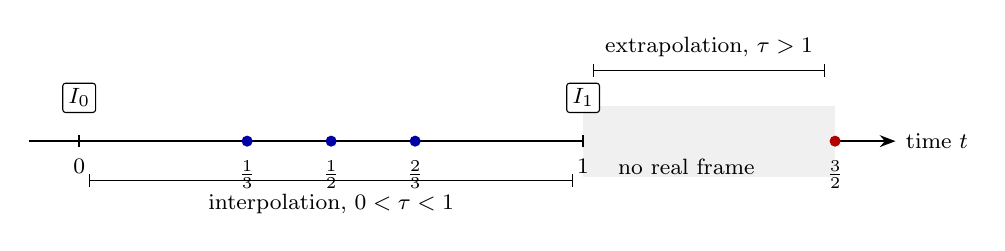
\begin{tikzpicture}[x=6.4cm, font=\footnotesize]
  \draw[thick, -{Stealth[length=2mm]}] (-0.1,0) -- (1.62,0) node[right] {time $t$};
  \fill[gray!12] (1,-0.45) rectangle (1.5,0.45);
  \draw[thick] (0,-0.08) -- (0,0.08);
  \draw[thick] (1,-0.08) -- (1,0.08);
  \node[draw, rounded corners=1pt, fill=white, inner sep=2pt] at (0,0.55) {$I_0$};
  \node[draw, rounded corners=1pt, fill=white, inner sep=2pt] at (1,0.55) {$I_1$};
  \node[below] at (0,-0.1) {$0$};
  \node[below] at (1,-0.1) {$1$};
  \foreach \x/\lab in {0.3333/{$\tfrac13$}, 0.5/{$\tfrac12$}, 0.6667/{$\tfrac23$}}{
    \fill[blue!65!black] (\x,0) circle (2pt);
    \node[below] at (\x,-0.12) {\lab};
  }
  \fill[red!70!black] (1.5,0) circle (2pt);
  \node[below] at (1.5,-0.12) {$\tfrac32$};
  \draw[|-|] (0.02,-0.5) -- (0.98,-0.5);
  \node[below] at (0.5,-0.55) {\footnotesize interpolation, $0<\tau<1$};
  \draw[|-|] (1.02,0.9) -- (1.48,0.9);
  \node[above] at (1.25,0.95) {\footnotesize extrapolation, $\tau>1$};
  \node[anchor=west, font=\footnotesize] at (1.05,-0.32) {no real frame};
\end{tikzpicture}
\caption{Time axis of the two generation modes with real frames $I_0$ and $I_1$. Interpolation (blue) places generated frames between the real frames, at $\tau=\tfrac12$ or at the two positions of 3x generation. Extrapolation (red) places a generated frame after $I_1$ at $\tau=\tfrac32$ using only frames at or before time 1. The shaded interval has no real frame.}\label{fig:bg-tau}
\end{figure}

\paragraph{Intermediate flows.} The generator needs the motion from each real frame to the intermediate time $\tau$, which is $F_{\tau\to0}$ and $F_{\tau\to1}$ as defined in \cref{sec:bg-motion}. Under constant velocity, a surface point moves as $\mathbf p(\tau)=\mathbf p_0+\tau\mathbf v$, where $\mathbf v$ is its displacement from time 0 to time 1, so that $\mathbf p_1=\mathbf p_0+\mathbf v$. Its displacement from $I_1$ to $I_0$ is $M_1=-\mathbf v$, and therefore
\begin{equation}
F_{\tau\to0}=\tau M_1,\qquad F_{\tau\to1}=(\tau-1)M_1,\label{eq:bg-linear}
\end{equation}
which are the linear-motion priors of the frame generator. To see this, note $F_{\tau\to0}=\mathbf p_0-\mathbf p(\tau)=-\tau\mathbf v=\tau M_1$, and $F_{\tau\to1}=\mathbf p_1-\mathbf p(\tau)=(1-\tau)\mathbf v=(\tau-1)M_1$. The code evaluates $M_1$ at the target pixel rather than at the moving point, which is exact when the motion field is locally constant.

\paragraph{Coarse-to-fine estimation.} The intermediate flows come from an IFNet with the design of RIFE 4.26 \cite{huang2022rife}. It is a chain of blocks, each working at a fraction $1/s_k$ of the input resolution, with scales $16,8,4,2,1$ for the five blocks of the full network. Each block predicts a blend logit and an update to the flow at its own resolution. The update is resampled to full resolution and multiplied by $s_k$, because a displacement in pixels scales with resolution, so
\begin{equation}
F^{(k)}=F^{(k-1)}+s_k\,\mathcal U_{s_k}\big(\tilde\Delta^{(k)}\big),\label{eq:bg-c2f}
\end{equation}
where $\tilde\Delta^{(k)}$ is the raw update of block $k$ and $\mathcal U_{s_k}$ is bilinear upsampling by $s_k$. The coarse blocks capture large motion at low cost, and the fine blocks add detail.

\paragraph{Blending.} The two warped frames are combined with a per-pixel blend $m\in[0,1]$, which is the sigmoid of the network's logit,
\begin{equation}
\hat I_\tau=m\odot\mathcal W(I_0,F_{\tau\to0})+(1-m)\odot\mathcal W(I_1,F_{\tau\to1}),\label{eq:bg-blend}
\end{equation}
where $\odot$ is the element-wise product. Where a surface is visible in only one real frame, the correct blend selects that frame, and this is how interpolation handles occlusions.

\paragraph{Resolution rule and cuts.} Flow is costly, so the generator estimates it at a reduced scale for tall frames. The flow scale is the largest $2^{-k}$ with $H\,2^{-k}\le L$, where $L$ is the flow limit of the tier, 576 or 1152 lines. At 1080p this gives 540 lines for $L=576$ and full resolution for $L=1152$. When two real frames come from different scenes, the flows and the blend describe no correspondence, so generation should not run. The code repeats $I_1$ in that case, as \cref{sec:bg-motion} describes. Interpolation also fails where the motion exceeds what the flow search can resolve, at disocclusions where the blend cannot choose, for particles and other motion without correspondence, and on overlays such as text and HUD elements that move differently from the scene.

\subsection{Frame budgets, pacing and latency}\label{sec:bg-latency}

\paragraph{Frame budget.} A display that refreshes $R$ times per second shows a new frame every $1000/R$ milliseconds. That is 16.7 ms at 60 Hz, 33.3 ms at 30 Hz and 8.3 ms at 120 Hz. A renderer that cannot finish a frame within the interval either presents it late or repeats the previous one, so every stage of the frame must fit the budget if the rate is to be sustained. The stages are a CPU update of $c$ ms, a GPU render of $r$ ms, the upscaling of $s$ ms, the frame generation of $g$ ms and the presentation of $p$ ms. In a GPU-bound loop the period is set by the GPU, so the period of a generating loop is $P=\max(c,\,r+s+g)$, the rule that \texttt{simulate\_latency} applies, and the CPU work starts just in time so that no frame waits in a queue.

\paragraph{Three quantities that differ.} Three measures are easily confused.
\begin{itemize}
\item The rendered frame rate is the number of real frames per second that the engine produces, which is $1000/P$ for a loop without generation.
\item The displayed frame rate is the number of frames presented per second, including generated frames. With one generated frame per real frame it is about twice the rendered rate, provided that generation does not lengthen the period, and in a GPU-bound loop it does lengthen it.
\item The input latency is the time from an input sample to the first photons of a frame that reflects it. The frame rate does not determine it.
\end{itemize}

\paragraph{Latency of interpolation and extrapolation.} Interpolation shows a generated frame between $I_{k-1}$ and $I_k$, which needs $I_k$ to exist. The real frame $I_k$ is therefore held until the generated frame has been shown, and it is shown about half a period later, so the input latency of a real frame rises by $g+P/2$. Extrapolation generates from past frames only, so a real frame is presented as soon as it is rendered and its latency does not change. The generated frame follows the real frame, and in the simulator it is presented half a period after it. \Cref{fig:bg-pacing} shows the presentation times that these rules give for one real frame in each mode.

\begin{figure}[!htbp]
\centering
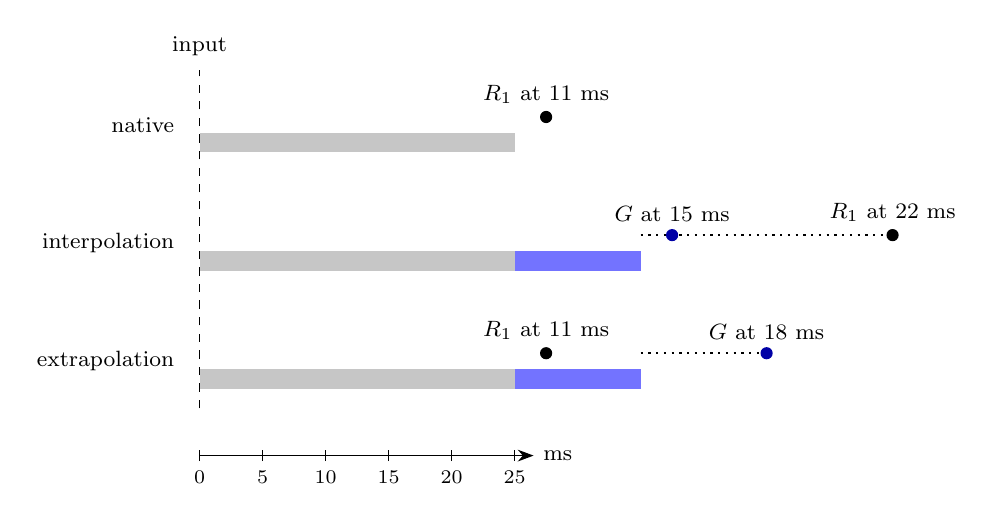
\begin{tikzpicture}[x=0.4cm, y=1cm, font=\footnotesize]
  \node[anchor=east] at (-0.5,3) {native};
  \node[anchor=east] at (-0.5,1.5) {interpolation};
  \node[anchor=east] at (-0.5,0) {extrapolation};
  \draw[dashed] (0,-0.6) -- (0,3.7);
  \node[anchor=south] at (0,3.75) {input};
  % native: render 0 to 10 ms, real frame shown at 11 ms
  \fill[gray!45] (0,2.65) rectangle (10,2.9);
  \fill[black] (11,3.1) circle (2.2pt);
  \node[anchor=south] at (11,3.15) {$R_1$ at 11 ms};
  % interpolation: render 0 to 10, generate 10 to 14, G shown at 15, R1 held and shown at 22
  \fill[gray!45] (0,1.15) rectangle (10,1.4);
  \fill[blue!55] (10,1.15) rectangle (14,1.4);
  \draw[dotted, thick] (14,1.6) -- (22,1.6);
  \fill[blue!65!black] (15,1.6) circle (2.2pt);
  \node[anchor=south] at (15,1.65) {$G$ at 15 ms};
  \fill[black] (22,1.6) circle (2.2pt);
  \node[anchor=south] at (22,1.65) {$R_1$ at 22 ms};
  % extrapolation: render 0 to 10, generate 10 to 14, R1 shown at 11, G shown at 18
  \fill[gray!45] (0,-0.35) rectangle (10,-0.1);
  \fill[blue!55] (10,-0.35) rectangle (14,-0.1);
  \fill[black] (11,0.1) circle (2.2pt);
  \node[anchor=south] at (11,0.15) {$R_1$ at 11 ms};
  \draw[dotted, thick] (14,0.1) -- (18,0.1);
  \fill[blue!65!black] (18,0.1) circle (2.2pt);
  \node[anchor=south] at (18,0.15) {$G$ at 18 ms};
  % time axis
  \draw[-{Stealth[length=2mm]}] (0,-1.2) -- (10.6,-1.2) node[right] {ms};
  \foreach \t in {0,5,10,15,20,25}{
    \draw (\t*0.4,-1.27) -- (\t*0.4,-1.13);
    \node[below, font=\scriptsize] at (\t*0.4,-1.27) {\t};
  }
\end{tikzpicture}
\caption{Schematic presentation times for one real frame and one generated frame, from the rules of the frame-pacing simulator, with render 10 ms, generation 4 ms and presentation 1 ms, and with CPU work and upscaling omitted. Grey bars are rendering, blue bars are generation and dotted lines are frames held for presentation. Interpolation holds the real frame until the generated frame is shown, so the real frame arrives 11 ms after its native time. The values are illustrative and are not measurements.}\label{fig:bg-pacing}
\end{figure}

The simulator's rules for the three modes are these. For a real frame, native latency is $c+r+s+p$, and interpolation adds $g+P/2$ to it. Extrapolation leaves it unchanged. For a generated frame, the camera latency, the time from input to the first displayed frame that reflects the camera, is $c+r+s+g+p$ for interpolation. For extrapolation it is $c+r+s+p+P/2$, or, with late latching, $g+p$.

\paragraph{Late latching.} Late latching samples the camera again as late as possible before a frame is generated, so that the generated frame moves with a newer camera. In the simulator this reduces the camera latency of an extrapolated frame to the generation time plus the presentation time, $g+p$. Late latching needs a camera input read just before generation, which the engine must provide.

\paragraph{Frame pacing and variable refresh.} Pacing means presenting frames at evenly spaced times. Uneven gaps are seen as stutter even when the mean rate is high, so the measure is the coefficient of variation of the gaps between presented frames, which the simulator reports as \texttt{frame\_gap\_cv}. A variable-refresh display presents each frame when it is ready within its supported range instead of at fixed intervals. The presentation time then equals the completion time, so irregular completion becomes irregular spacing unless the scheduler paces the frames. The simulator models such a display, which presents at the ready time.

\subsection{Metrics}\label{sec:bg-metrics}

Each metric compares an output frame $o$ with a reference frame $g$, both encoded RGB, and the references are exact because the test data are synthetic or come with ground truth. Metrics are computed per frame and per sample and then averaged. \Cref{tab:bg-metrics} summarises the direction and the limits of each measure, and the paragraphs below give the definitions exactly as the code computes them.

\begin{table}[!htbp]
\caption{Metrics of the supplement: range, direction and what each measure misses. Ranges are those of the definitions, and the cap of PSNR is the code's clamp}\label{tab:bg-metrics}
\begin{tabular*}{\columnwidth}{@{\extracolsep\fill}p{0.25\columnwidth}p{0.16\columnwidth}p{0.12\columnwidth}p{0.33\columnwidth}}
\toprule
Metric & Range & Better & What it misses \\
\midrule
PSNR (RGB, frame generation) & up to 100 dB & higher & Only the per-pixel squared error, so a blurred frame can score well \\
PSNR-Y (temporal super-resolution) & up to 100 dB & higher & Luma only, so chroma errors are ignored \\
SSIM & $-1$ to $1$ & higher & Local structure in $11\times11$ windows, nothing over time \\
LPIPS & non-negative & lower & Learned features of one network, nothing over time \\
FLIP (mean) & 0 to 1 & lower & A perceptual model with fixed viewing assumptions \\
IE & 0 to 255 & lower & A global error, like PSNR on another scale \\
Temporal-change error & non-negative & lower & Static errors that do not change in time, and it needs motion labels \\
Warp error & non-negative & lower & Agreement with the reference, so a consistently blurred output can score well \\
tOF & pixels & lower & Errors of the flow estimator, computed on every fourth frame \\
UI ghosting rate & 0 to 1 & lower & Errors below 10 percent of full scale and UI pixels only \\
Region PSNR & up to 100 dB & higher & Pixels outside the region, and the quality of the region mask \\
Gated share & 0 to 1 & lower on cut-free clips & Cuts that the gate misses, since the clips contain none \\
\botrule
\end{tabular*}
\end{table}

\paragraph{PSNR.} With a mask $M(\mathbf p)\in\{0,1\}$, the masked mean squared error and the PSNR in decibels are
\begin{equation}
\mathrm{MSE}_M=\frac{\sum_{\mathbf p}\sum_{c}M(\mathbf p)\big(o_c(\mathbf p)-g_c(\mathbf p)\big)^2}{\max\!\big(\sum_{\mathbf p}\sum_{c}M(\mathbf p),\,1\big)},\qquad \mathrm{PSNR}=10\log_{10}\frac{1}{\max(\mathrm{MSE}_M,\,10^{-10})},\label{eq:bg-psnr}
\end{equation}
where $c$ runs over the three channels and $M\equiv1$ gives the plain PSNR. The clamp caps the PSNR at 100 dB. Higher is better.

\paragraph{PSNR-Y.} The same formula is applied to $Y$ of Eq.~(\ref{eq:bg-luma}), after removing the $s$ outermost pixels of the high-resolution frame on each side (\texttt{psnr} with \texttt{border} $=s$). Because $Y$ is $219/255$ times the full-range luma plus a constant, the PSNR-Y of an error is $20\log_{10}(255/219)\approx1.32$ dB higher than the PSNR of the full-range luma with the same error. This offset is constant, so the differences between methods are unaffected.

\paragraph{SSIM.} The structural similarity index of \cite{wang2004ssim} compares local means, variances and covariance under a Gaussian window,
\begin{equation}
\mathrm{SSIM}(\mathbf p)=\frac{(2\mu_o\mu_g+C_1)(2\sigma_{og}+C_2)}{(\mu_o^2+\mu_g^2+C_1)(\sigma_o^2+\sigma_g^2+C_2)},\qquad C_1=(0.01)^2,\quad C_2=(0.03)^2,\label{eq:bg-ssim}
\end{equation}
where $\mu$, $\sigma^2$ and $\sigma_{og}$ are the local mean, variance and covariance under an $11\times11$ Gaussian window with $\sigma=1.5$ whose weights sum to one. The window is evaluated only where it lies inside the image (a valid convolution), so the map is 10 pixels smaller in each direction. The score is the mean over the map and over channels, lies in $[-1,1]$ and is higher for a better match. The temporal super-resolution network scores $Y$, and the frame generator scores each RGB channel.

\paragraph{LPIPS.} The learned perceptual distance \cite{zhang2018lpips} is
\begin{equation}
d_{\text{LPIPS}}(o,g)=\sum_{l}\frac{1}{H_lW_l}\sum_{h,w}\big\|\mathbf w_l\odot\big(\hat\phi^l_{hw}(o)-\hat\phi^l_{hw}(g)\big)\big\|_2^2,\label{eq:bg-lpips}
\end{equation}
where $\hat\phi^l_{hw}$ is the unit-normalised feature vector of AlexNet layer $l$ at position $(h,w)$, $\mathbf w_l$ are learned per-channel weights and $H_l\times W_l$ is the layer's size. Lower is better. The code calls the \texttt{lpips} package with AlexNet and \texttt{normalize=True}. If that package cannot build the network, \texttt{LPIPSAlex} builds the same network from torchvision's ImageNet AlexNet weights and the version 0.1 linear weights of the package, and maps the inputs from $[0,1]$ to $[-1,1]$ with $2x-1$ (\texttt{load\_lpips}). The temporal super-resolution evaluation computes LPIPS on every fourth frame, and the frame generator computes it on every sample.

\paragraph{FLIP.} FLIP \cite{andersson2020flip} is a perceptual difference evaluator that produces a per-pixel error map. The code calls \texttt{flip\_evaluator.evaluate} with the LDR traits and takes element 1 of its result (\texttt{flip\_error}). The official example of the package unpacks the result as the error map, the mean FLIP error and the parameters, so element 1 is the mean error. The traits string in the official example is \texttt{"HDR"}, so the LDR setting used by the code is not checked against an example here. The temporal super-resolution notebook calls the function on one frame pair, and FLIP is therefore a single-frame measure in this supplement. Lower is better.

\paragraph{Interpolation error (IE).} The code computes
\begin{equation}
\mathrm{IE}=255\sqrt{\frac{1}{3HW}\sum_{\mathbf p}\sum_{c}\big(o_c(\mathbf p)-g_c(\mathbf p)\big)^2},\label{eq:bg-ie}
\end{equation}
which is the root-mean-square difference on the 0 to 255 scale (\texttt{interpolation\_error}). Lower is better. The measure of Baker et al.\ \cite{baker2011middlebury} is the root-mean-square difference between the ground-truth and the interpolated image, taken over the RGB channels of every pixel for colour, and the 0 to 255 scale is this code's convention. \texttt{fg\_metrics} computes IE for every frame-generation sample, and the Middlebury interpolation set \cite{baker2011middlebury} is one of the frame-generation suites, with the code naming the measure after that benchmark.

\paragraph{Temporal-change error.} This measure compares the frame-to-frame change of the output with that of the reference along the reference motion. Let $m_t$ be the motion vector of frame $t$ and $v_t$ the validity mask. Define $D_o=o_t-\mathcal W(o_{t-1},m_t)$ and $D_g=g_t-\mathcal W(g_{t-1},m_t)$. The error is
\begin{equation}
e_{\text{tc}}(t)=\frac{\sum_{\mathbf p}v_t(\mathbf p)\,\tfrac13\sum_c\big|D_o(\mathbf p,c)-D_g(\mathbf p,c)\big|}{\max\big(\sum_{\mathbf p}v_t(\mathbf p),\,1\big)}.\label{eq:bg-tce}
\end{equation}
It is computed for frames $t\ge1$ of samples whose motion labels are exact or from RAFT (\texttt{temporal\_change\_error}). Lower is better. Flicker and ghosting appear as change where the reference has none, and the reference's own change is subtracted. A stable output with a constant error relative to the reference scores zero, so the measure does not see static errors. Its value also depends on the quality of the motion labels, which are less reliable for RAFT labels than for exact ones.

\paragraph{Warp error.} The warp error uses the same warp but compares the output with itself,
\begin{equation}
e_{w}(t)=\frac{\sum_{\mathbf p}v_t(\mathbf p)\,\tfrac13\sum_c\big|o_t(\mathbf p,c)-\mathcal W(o_{t-1},m_t)(\mathbf p,c)\big|}{\max\big(\sum_{\mathbf p}v_t(\mathbf p),\,1\big)},\label{eq:bg-we}
\end{equation}
and it is computed only for samples with exact motion labels (\texttt{warping\_error}). Lower is better. It measures the consistency of the output along true motion and does not look at the reference, so a consistently blurred output can score well. It should be read together with the temporal-change error.

\paragraph{tOF.} The temporal optical-flow difference of \cite{chu2020tecogan} compares the RAFT-Small flow of the output with the flow of the reference,
\begin{equation}
\mathrm{tOF}(t)=\frac{1}{HW}\sum_{\mathbf p}\big\|F^{\text{RAFT}}_{o_t\to o_{t-1}}(\mathbf p)-F^{\text{RAFT}}_{g_t\to g_{t-1}}(\mathbf p)\big\|_2,\label{eq:bg-tof}
\end{equation}
in pixels (\texttt{tof}). It is computed for $t\ge1$ with $t$ divisible by 4 (the \texttt{lpips\_every} setting). Lower is better. Flicker changes the estimated flow, so the measure detects it, but errors of RAFT itself enter both terms and cannot be separated from the output's errors. The file also defines \texttt{tlp}, the LPIPS analogue of tOF, but no evaluation function calls it, so it is not reported.

\paragraph{UI ghosting rate.} Let $U=\{\mathbf p: M_{\text{UI}}(\mathbf p)>0.5\}$, where $M_{\text{UI}}=\max(\alpha_0,\alpha_1)$ combines the UI coverage of the two real frames. The ghosting rate is
\begin{equation}
R_{\text{ghost}}=\frac{\big|\{\mathbf p\in U:\ \max_c|o_c(\mathbf p)-g_c(\mathbf p)|>0.1\}\big|}{\max(|U|,1)},\label{eq:bg-ghost}
\end{equation}
which is the share of UI pixels whose error exceeds 10 percent of full scale in any channel (\texttt{fg\_metrics}). It is defined only for samples that contain UI. Lower is better. It counts errors above the threshold and ignores their size.

\paragraph{Region PSNR.} Eq.~(\ref{eq:bg-psnr}) is restricted to five masks. The disocclusion mask is $1-v_t$ for $t\ge1$. The detail mask is the top 15 percent of the reference luma gradient, where the central differences $\partial_xY(\mathbf p)=Y(\mathbf p+\mathbf e_x)-Y(\mathbf p-\mathbf e_x)$ and $\partial_yY$ give a magnitude $\sqrt{\partial_x Y^2+\partial_y Y^2}$, thresholded at the 85th percentile of each frame (\texttt{hf\_mask}). The particle mask is the reactive mask, upsampled to output resolution and thresholded at 0.1. The UI mask is $U$. The occluded mask of the frame generator is $1-v_{\tau\to1}$, the target pixels that are not visible in $I_1$. Each region PSNR is reported only when its mask covers more than 50 pixels. Higher is better. The measure ignores all pixels outside its mask, and the disocclusion mask is only as good as the validity labels. Where a sample has no motion labels, $v$ is zero and the disocclusion mask covers the whole frame (\texttt{sr\_frame\_metrics}). When RAFT is available, every frame after the first of a real clip has labels, so the all-pixel case arises only without RAFT.

\paragraph{Gated share.} The cut gate skips generation and repeats the newest real frame where the score of Eq.~(\ref{eq:bg-cut}), with the motion term when a motion vector is available, exceeds its threshold (\texttt{cut\_gate}). The test clips contain no cuts, so every gated real sample is a false alarm, and the gated share is the fraction of real samples on which the gate fires. Lower is better on cut-free clips. The gated share says nothing about cuts that the gate misses, because the clips contain none.

\section{Data, copy detection and leakage control}\label{sec:data}

The data pipeline notebook builds the single manifest that both training notebooks read. It has three jobs. It gathers public stills and video sequences, it removes near copies so that no test content reaches training, and it records for every item its leakage group, its split and the locations of its frames, motion and depth. \cref{M-sec:data} of the article summarises the procedure. This section gives the complete method, every threshold, and every saved output of the notebook.

Every result here comes from one saved run of the pipeline. A result that rests on one run carries the \Preliminary{} tag, because a run with other seeds or other caps can change the counts. Descriptions of what the code does carry no tag. Every count and threshold quoted in this section is a generated result key, except for design constants that are written in the code, and each of these is quoted from the code.

Four terms are used throughout. An \emph{item} is one still image or one video sequence, and it is the unit of the manifest. A \emph{keyframe} is a decoded frame of an item that is used for statistics and copy detection. A \emph{leakage group} is a set of items that must never be split between training, validation and test, such as the frames of one video or one rendered scene. A \emph{duplicate edge} joins two keyframes that show the same picture. Each item ends with one split: train, val or test for items that are used, drop for an item removed because it is a near copy of test content or shares a group with it, and filtered for an item removed by a quality rule.

The notebook runs eleven timed stages in this order: Kaggle discovery, Hugging Face materialisation, keyframe statistics, quality filters, perceptual hashes, DINOv2 embeddings, SIFT features, threshold calibration, candidate search and verification, the leakage-safe split with its audit, and the manifest with the dataset card. \cref{tab:data-stages} gives the time of each stage.

\begin{table}[!htbp]
\caption{Stage times of the saved run, in minutes}\label{tab:data-stages}
\footnotesize
\begin{tabular}{@{}lr@{}}
\toprule
Stage & Minutes \\
\midrule
Kaggle discovery & \Res{data.stage_times.kaggle_discovery.minutes} \\
Hugging Face materialisation & \Res{data.stage_times.hf_materialisation.minutes} \\
Keyframe statistics & \Res{data.stage_times.keyframe_stats.minutes} \\
Filters & \Res{data.stage_times.filters.minutes} \\
Perceptual hashes & \Res{data.stage_times.hashes.minutes} \\
Embeddings & \Res{data.stage_times.embeddings.minutes} \\
Local features (SIFT) & \Res{data.stage_times.local_features.minutes} \\
Calibration & \Res{data.stage_times.calibration.minutes} \\
Duplicate search and verification & \Res{data.stage_times.duplicate_search.minutes} \\
Split and audit & \Res{data.stage_times.split_and_audit.minutes} \\
Manifest & \Res{data.stage_times.manifest.minutes} \\
\bottomrule
\end{tabular}
\end{table}

\subsection{Source datasets}\label{sec:data-sources}

The pipeline reads two hosts. The Kaggle datasets are attached to the notebook and read from the read-only input mount, which the code locates by the dataset's owner and slug. The Hugging Face (HF) datasets are read over HTTPS. The code keeps one connection alive per thread, checks the length of every range read, and retries failed reads. A zip member is read through range requests without downloading the archive, and the GameIR tars are read as one sequential stream that stops once the clip cap is reached. The Vimeo-1080p step is different. It downloads each named parquet shard in full, reads the MP4 files inside it, and deletes the shard, so the notebook's statement that the pipeline makes no full archive downloads does not hold for that source. Each source is optional. A source that fails is logged and skipped, and the run continues.

\Cref{tab:data-sources} lists the eleven sources. The sizes are the means of the saved keyframe sizes. The licence column repeats the strings written in the code. The upstream licence pages were not checked for this section, so these are the code's statements and not checked legal facts. The code marks the game captures as needing a check for each use, and it gives the Vimeo-1080p licence as unspecified. The notebook's dataset card refers to \texttt{RESEARCH.md} for commercial-use restrictions. That file exists in the repository, but its contents were not checked for this section. The licences need checking against each upstream page before any release.

\begin{table}[!htbp]
\caption{Source datasets, as the code reads them. Sizes are mean keyframe widths and heights in pixels from the saved keyframe table. Licence strings are the code's statements, not checked against upstream pages}\label{tab:data-sources}
\footnotesize
\begin{tabular}{@{}p{2.4cm}p{3.2cm}p{3.6cm}p{1.9cm}@{}}
\toprule
Source & Host and identifier & Content and ground truth & Size (px) \\
\midrule
DIV2K & Kaggle \texttt{soumikrakshit/\allowbreak div2k-\allowbreak high-\allowbreak resolution-\allowbreak images} & Photographs, still, no motion, and validation images pinned to test & \Res{data.keyframe_stats.div2k.width.mean}$\times$\Res{data.keyframe_stats.div2k.height.mean} \\
Flickr2K & Kaggle \texttt{daehoyang/flickr2k} & Photographs, still, train only & \Res{data.keyframe_stats.flickr2k.width.mean}$\times$\Res{data.keyframe_stats.flickr2k.height.mean} \\
Game stills & HF \texttt{ericphann/\allowbreak video-\allowbreak game-\allowbreak super-\allowbreak resolution} & 1080p game captures, still, with \texttt{training-hr} as train and \texttt{test-hr} as test & \Res{data.keyframe_stats.game_stills.width.mean}$\times$\Res{data.keyframe_stats.game_stills.height.mean} \\
REDS & Kaggle \texttt{amithkesavmrajagiri/\allowbreak reds-\allowbreak dataset} & 720p video clips, no motion labels, train only & \Res{data.keyframe_stats.reds.width.mean}$\times$\Res{data.keyframe_stats.reds.height.mean} \\
Vimeo-90K septuplets & Kaggle \texttt{wangsally/\allowbreak vimeo-\allowbreak 90k-\allowbreak 7} & Seven-frame video sequences, no motion labels, train only & \Res{data.keyframe_stats.vimeo_septuplet.width.mean}$\times$\Res{data.keyframe_stats.vimeo_septuplet.height.mean} \\
Vimeo-90K triplets & Kaggle \texttt{chenshu123/\allowbreak vimeo-\allowbreak triplet} & Three-frame sequences from the official test list, test only & \Res{data.keyframe_stats.vimeo_triplet.width.mean}$\times$\Res{data.keyframe_stats.vimeo_triplet.height.mean} \\
MPI Sintel & Kaggle \texttt{artemmmtry/\allowbreak mpi-\allowbreak sintel-\allowbreak dataset} & Rendered scenes with exact forward flow and occlusion masks, with \texttt{market} and \texttt{cave} as test & \Res{data.keyframe_stats.sintel.width.mean}$\times$\Res{data.keyframe_stats.sintel.height.mean} \\
Vid4 & Kaggle \texttt{uom200647r/\allowbreak vid4-\allowbreak dataset} & Video clips, no motion labels, test only & \Res{data.keyframe_stats.vid4.width.mean}$\times$\Res{data.keyframe_stats.vid4.height.mean} \\
TartanAir & HF \texttt{theairlabcmu/tartanair} & Rendered scenes with exact forward flow, occlusion masks and depth, with two environments as test & \Res{data.keyframe_stats.tartanair.width.mean}$\times$\Res{data.keyframe_stats.tartanair.height.mean} \\
GameIR & HF \texttt{LLLebin/GameIR} & CARLA and Unreal Engine 4 game renders at 1440p and 720p, with depth and no exact flow, and the test tar as test & \Res{data.keyframe_stats.gameir.width.mean}$\times$\Res{data.keyframe_stats.gameir.height.mean} \\
Vimeo-1080p & HF \texttt{danjacobellis/\allowbreak vimeo1080p} & 1080p MP4 videos, no motion labels, validation shard as test & \Res{data.keyframe_stats.vimeo1080p.width.mean}$\times$\Res{data.keyframe_stats.vimeo1080p.height.mean} \\
\bottomrule
\end{tabular}
\end{table}

The roles are set by the code. The test items are the DIV2K validation images, the Vid4 clips, the official Vimeo-90K triplet test list, the Sintel \texttt{market} and \texttt{cave} scene families, the two TartanAir test environments, the GameIR test tar and the Vimeo-1080p validation shard. Every other item is a training candidate, and the split of \cref{sec:data-split} decides whether it ends in train or val. The sources are DIV2K \cite{agustsson2017div2k}, REDS \cite{nah2019reds}, Vimeo-90K \cite{xue2019vimeo}, MPI Sintel \cite{butler2012sintel}, TartanAir \cite{wang2020tartanair}, GameIR \cite{zhou2024gameir}, Vid4 \cite{liu2014vid4} and CARLA \cite{dosovitskiy2017carla}, which the GameIR renders use. The DIV2K training and validation counts follow the published split of 800 training and 100 validation images, which the catalogue reproduces.

Two sources carry ground truth beyond the frames themselves. Sintel and TartanAir give exact forward optical flow and occlusion masks, and TartanAir and GameIR give depth. These are the only sources the training uses as exact labels, and the rest rely on the frames, either as targets or through the RAFT teacher flow of \cref{sec:data-synth-tsr}.

\subsection{Discovery and catalogue}\label{sec:data-discovery}

Discovery runs once per attached Kaggle dataset, and the seven Kaggle sources run in parallel threads. For each dataset the code lists files with \texttt{sampled\_walk}. This function keeps a frontier of directories, expands one directory chosen at random at each step, and lists every file in that directory completely. A listed sequence folder is therefore never cut in half. Listing stops when the file cap is reached, which is \Res{data.config.cfg.list_cap_files} files by default. The REDS and Vimeo-90K septuplet listings reached the cap before the walk finished, so their listings are incomplete, and the other sources listed completely.

A file is kept only if its path has no token that marks a degraded copy or a non-colour pass. The degraded tokens are \texttt{lr}, \texttt{lq}, \texttt{bicubic}, \texttt{blur}, \texttt{x2} to \texttt{x4} and similar, and the non-colour tokens include \texttt{flow}, \texttt{depth}, \texttt{occlusions}, \texttt{mask} and \texttt{albedo}. Tokens are the lower-case pieces of the directory and file names. For video, if any path carries a high-resolution token (\texttt{hr}, \texttt{gt}, \texttt{original} or \texttt{groundtruth}), only those paths are kept. Stills become one item each. Video frames become one item per folder, and the leakage group is the folder name for level 1 sources and the parent folder for level 2 sources. A folder with fewer than three frames is skipped. For Sintel, the group is the scene prefix (for example \texttt{market}), and each item carries the forward flow files and the occlusion masks that match its frames. The Vimeo-90K triplet clips are read directly from the official test list, and up to 1,000 of them are sampled with the seed.

\Cref{tab:data-discovery} reports the discovery per source. The listed and kept counts are file counts, and the items are the sequences or stills that survived the path rules. Sintel lists \Res{data.discovery_kaggle.sintel.listed} files and keeps \Res{data.discovery_kaggle.sintel.kept_files} of them, and the difference comes from files that the path rules remove, such as non-colour passes and masks. \Preliminary

\begin{table}[!htbp]
\caption{Kaggle discovery per source. Files are counted after the directory walk and after the path rules. The REDS and Vimeo-90K septuplet listings reached their cap, so their file counts are lower bounds}\label{tab:data-discovery}
\footnotesize
\begin{tabular}{@{}lrrrrr@{}}
\toprule
Source & Files listed & Files kept & Directories listed & Items & Test items \\
\midrule
DIV2K & \Res{data.discovery_kaggle.div2k.listed} & \Res{data.discovery_kaggle.div2k.kept_files} & \Res{data.discovery_kaggle.div2k.dirs_listed} & \Res{data.discovery_kaggle.div2k.items} & \Res{data.discovery_kaggle.div2k.test_items} \\
Flickr2K & \Res{data.discovery_kaggle.flickr2k.listed} & \Res{data.discovery_kaggle.flickr2k.kept_files} & \Res{data.discovery_kaggle.flickr2k.dirs_listed} & \Res{data.discovery_kaggle.flickr2k.items} & \Res{data.discovery_kaggle.flickr2k.test_items} \\
REDS & \Res{data.discovery_kaggle.reds.listed} & \Res{data.discovery_kaggle.reds.kept_files} & \Res{data.discovery_kaggle.reds.dirs_listed} & \Res{data.discovery_kaggle.reds.items} & \Res{data.discovery_kaggle.reds.test_items} \\
Vimeo-90K septuplets & \Res{data.discovery_kaggle.vimeo_septuplet.listed} & \Res{data.discovery_kaggle.vimeo_septuplet.kept_files} & \Res{data.discovery_kaggle.vimeo_septuplet.dirs_listed} & \Res{data.discovery_kaggle.vimeo_septuplet.items} & \Res{data.discovery_kaggle.vimeo_septuplet.test_items} \\
Vimeo-90K triplets & \Res{data.discovery_kaggle.vimeo_triplet.listed} & \Res{data.discovery_kaggle.vimeo_triplet.kept_files} & \Res{data.discovery_kaggle.vimeo_triplet.dirs_listed} & \Res{data.discovery_kaggle.vimeo_triplet.items} & \Res{data.discovery_kaggle.vimeo_triplet.test_items} \\
MPI Sintel & \Res{data.discovery_kaggle.sintel.listed} & \Res{data.discovery_kaggle.sintel.kept_files} & \Res{data.discovery_kaggle.sintel.dirs_listed} & \Res{data.discovery_kaggle.sintel.items} & \Res{data.discovery_kaggle.sintel.test_items} \\
Vid4 & \Res{data.discovery_kaggle.vid4.listed} & \Res{data.discovery_kaggle.vid4.kept_files} & \Res{data.discovery_kaggle.vid4.dirs_listed} & \Res{data.discovery_kaggle.vid4.items} & \Res{data.discovery_kaggle.vid4.test_items} \\
\bottomrule
\end{tabular}
\end{table}

The Hugging Face sources are materialised next, into the data root, and each one follows its own access rule. Game stills are a random sample of the listed PNG files in the training and test folders, with the seed. TartanAir is read per environment. For each environment the code reads the first trajectory of the Easy difficulty zips, takes a contiguous run of frames starting at one quarter of the way along the trajectory, and stores RGB, depth, forward flow and a validity mask. The validity mask is white where the TartanAir mask is zero, which means a valid correspondence. The run stops early if a flow or mask file is missing. Each run is cut into sequences of 24 frames, which is the TartanAir sequence length in the configuration. GameIR keeps the 1440p and 720p renders and the depth of every clip with at least three high-resolution frames and a matching low-resolution frame. The code records a frame stride of ten rendered frames for these clips, but it does not subsample them, so the frames are whatever the mini tar holds. Vimeo-1080p writes each MP4 to disk, counts its frames, and keeps videos with at least eight frames.

\Cref{tab:data-catalogue} is the catalogue, which counts items, frames, exact-motion items and depth items for each source and role. The counts are taken before the quality filters, so they describe what was materialised. \Preliminary

\begin{table}[!htbp]
\caption{Catalogue before filtering, by source, kind and role. Exact motion counts items with exact forward flow and depth counts items with depth. Each row is one source and role that exists in the run}\label{tab:data-catalogue}
\footnotesize
\begin{tabular}{@{}llrrrrr@{}}
\toprule
Source & Role & Items & Frames & Exact motion & Depth \\
\midrule
DIV2K & train & \Res{data.catalogue_summary.div2k.still.train.items} & \Res{data.catalogue_summary.div2k.still.train.frames} & \Res{data.catalogue_summary.div2k.still.train.exact_motion} & \Res{data.catalogue_summary.div2k.still.train.with_depth} \\
DIV2K & test & \Res{data.catalogue_summary.div2k.still.test.items} & \Res{data.catalogue_summary.div2k.still.test.frames} & \Res{data.catalogue_summary.div2k.still.test.exact_motion} & \Res{data.catalogue_summary.div2k.still.test.with_depth} \\
Flickr2K & train & \Res{data.catalogue_summary.flickr2k.still.train.items} & \Res{data.catalogue_summary.flickr2k.still.train.frames} & \Res{data.catalogue_summary.flickr2k.still.train.exact_motion} & \Res{data.catalogue_summary.flickr2k.still.train.with_depth} \\
Game stills & train & \Res{data.catalogue_summary.game_stills.still.train.items} & \Res{data.catalogue_summary.game_stills.still.train.frames} & \Res{data.catalogue_summary.game_stills.still.train.exact_motion} & \Res{data.catalogue_summary.game_stills.still.train.with_depth} \\
Game stills & test & \Res{data.catalogue_summary.game_stills.still.test.items} & \Res{data.catalogue_summary.game_stills.still.test.frames} & \Res{data.catalogue_summary.game_stills.still.test.exact_motion} & \Res{data.catalogue_summary.game_stills.still.test.with_depth} \\
GameIR & train & \Res{data.catalogue_summary.gameir.seq.train.items} & \Res{data.catalogue_summary.gameir.seq.train.frames} & \Res{data.catalogue_summary.gameir.seq.train.exact_motion} & \Res{data.catalogue_summary.gameir.seq.train.with_depth} \\
GameIR & test & \Res{data.catalogue_summary.gameir.seq.test.items} & \Res{data.catalogue_summary.gameir.seq.test.frames} & \Res{data.catalogue_summary.gameir.seq.test.exact_motion} & \Res{data.catalogue_summary.gameir.seq.test.with_depth} \\
REDS & train & \Res{data.catalogue_summary.reds.seq.train.items} & \Res{data.catalogue_summary.reds.seq.train.frames} & \Res{data.catalogue_summary.reds.seq.train.exact_motion} & \Res{data.catalogue_summary.reds.seq.train.with_depth} \\
Vimeo-90K septuplets & train & \Res{data.catalogue_summary.vimeo_septuplet.seq.train.items} & \Res{data.catalogue_summary.vimeo_septuplet.seq.train.frames} & \Res{data.catalogue_summary.vimeo_septuplet.seq.train.exact_motion} & \Res{data.catalogue_summary.vimeo_septuplet.seq.train.with_depth} \\
Vimeo-90K triplets & test & \Res{data.catalogue_summary.vimeo_triplet.seq.test.items} & \Res{data.catalogue_summary.vimeo_triplet.seq.test.frames} & \Res{data.catalogue_summary.vimeo_triplet.seq.test.exact_motion} & \Res{data.catalogue_summary.vimeo_triplet.seq.test.with_depth} \\
MPI Sintel & train & \Res{data.catalogue_summary.sintel.seq.train.items} & \Res{data.catalogue_summary.sintel.seq.train.frames} & \Res{data.catalogue_summary.sintel.seq.train.exact_motion} & \Res{data.catalogue_summary.sintel.seq.train.with_depth} \\
MPI Sintel & test & \Res{data.catalogue_summary.sintel.seq.test.items} & \Res{data.catalogue_summary.sintel.seq.test.frames} & \Res{data.catalogue_summary.sintel.seq.test.exact_motion} & \Res{data.catalogue_summary.sintel.seq.test.with_depth} \\
TartanAir & train & \Res{data.catalogue_summary.tartanair.seq.train.items} & \Res{data.catalogue_summary.tartanair.seq.train.frames} & \Res{data.catalogue_summary.tartanair.seq.train.exact_motion} & \Res{data.catalogue_summary.tartanair.seq.train.with_depth} \\
TartanAir & test & \Res{data.catalogue_summary.tartanair.seq.test.items} & \Res{data.catalogue_summary.tartanair.seq.test.frames} & \Res{data.catalogue_summary.tartanair.seq.test.exact_motion} & \Res{data.catalogue_summary.tartanair.seq.test.with_depth} \\
Vid4 & test & \Res{data.catalogue_summary.vid4.seq.test.items} & \Res{data.catalogue_summary.vid4.seq.test.frames} & \Res{data.catalogue_summary.vid4.seq.test.exact_motion} & \Res{data.catalogue_summary.vid4.seq.test.with_depth} \\
Vimeo-1080p & train & \Res{data.catalogue_summary.vimeo1080p.seq.train.items} & \Res{data.catalogue_summary.vimeo1080p.seq.train.frames} & \Res{data.catalogue_summary.vimeo1080p.seq.train.exact_motion} & \Res{data.catalogue_summary.vimeo1080p.seq.train.with_depth} \\
Vimeo-1080p & test & \Res{data.catalogue_summary.vimeo1080p.seq.test.items} & \Res{data.catalogue_summary.vimeo1080p.seq.test.frames} & \Res{data.catalogue_summary.vimeo1080p.seq.test.exact_motion} & \Res{data.catalogue_summary.vimeo1080p.seq.test.with_depth} \\
\bottomrule
\end{tabular}
\end{table}

\Cref{fig:data-catalogue} shows the same catalogue as plots. The left panel stacks the items of each source by role. The Vimeo-90K septuplets are the largest source by items, and the Vimeo-90K triplets, which are test only, form the largest block of test items. The right panel gives the frame totals on a logarithmic axis, which spans about three decades. The Vimeo-90K and Vimeo-1080p sources carry the most frames, and the sources with exact motion and depth are a small share of the frames. \Observation

\begin{figure}[!htbp]
\centering
\includegraphics[width=0.9\textwidth]{\DataOut/plots/catalogue.png}
\caption{Catalogue before filtering. Left: items per source, stacked by role. Right: frames on a logarithmic axis, and the sequences with exact motion and with depth. Both panels come from the notebook's catalogue cell}\label{fig:data-catalogue}
\end{figure}

\subsection{Quality filtering}\label{sec:data-filters}

Quality is judged on statistics of the keyframes, which \cref{sec:data-keyframes} defines. For each keyframe the code computes the grey mean and the grey standard deviation of the full-resolution frame, where grey is the mean of the red, green and blue values. It also computes the letterbox fraction $\lambda$. A row counts as dark when its mean grey value is below 8. The letterbox fraction is the number of dark rows at the top plus the number at the bottom, divided by the frame height. The sharpness is computed on the 256 by 256 thumbnail $g$. The code applies the four-neighbour Laplacian
\begin{equation}
L(x,y)=4g(x,y)-g(x-1,y)-g(x+1,y)-g(x,y-1)-g(x,y+1),\label{eq:data-sharp}
\end{equation}
and takes the variance of $L$ over the interior pixels as the sharpness. A flat image has a small variance of $L$, and a sharp image has a large one. The colourfulness measure of each keyframe uses the opponent channels $rg=R-G$ and $yb=\tfrac{1}{2}(R+G)-B$, and its value is
\begin{equation}
C=\sqrt{\sigma_{rg}^2+\sigma_{yb}^2}+0.3\sqrt{\mu_{rg}^2+\mu_{yb}^2},\label{eq:data-colour}
\end{equation}
where $\sigma$ and $\mu$ are the standard deviation and mean over the thumbnail. This is the colourfulness index of Hasler and S{\"u}sstrunk \cite{hasler2003measuring}. The colourfulness is recorded but no rule uses it.

An item is rejected if it has any of five reasons. The first is a decode error, which means a keyframe could not be read. The second is a side below 256 pixels, which means any keyframe with a smaller width or height than 256. The third is flatness, which means the median grey standard deviation over the item's keyframes is below 8. The fourth is letterboxing, which means the median letterbox fraction is above 0.35. The fifth is blur, which means the median sharpness is below 20 for stills and below 5 for sequences. Stills are judged on their one keyframe. Sequences are judged on the median of their keyframes, so one dark shot or one fade does not reject a whole video. A rejected item keeps its row in the manifest with split filtered and is left out of the duplicate search, so the decision can be audited. The manifest does not record which rule fired. The notebook printed these reasons, but the printed output was not saved, so this section gives no per-reason counts.

\Cref{tab:data-split-source} gives the per-source totals. In this run \Res{data.summary.filtered} of \Res{data.summary.items} items were filtered. Filtering removed \Res{data.split_by_source.vimeo_septuplet.filtered} Vimeo-90K septuplet items and \Res{data.split_by_source.game_stills.filtered} game-still items, and the remaining filtered items came from the triplet and Vimeo-1080p sources. The filtered items are a small share of all items. \Preliminary

\begin{table}[!htbp]
\caption{Split per source. Drop means removed as a near copy of test content or as a member of a test group, and filtered means removed by a quality rule}\label{tab:data-split-source}
\footnotesize
\begin{tabular}{@{}lrrrrr@{}}
\toprule
Source & Train & Val & Test & Drop & Filtered \\
\midrule
DIV2K & \Res{data.split_by_source.div2k.train} & \Res{data.split_by_source.div2k.val} & \Res{data.split_by_source.div2k.test} & \Res{data.split_by_source.div2k.drop} & \Res{data.split_by_source.div2k.filtered} \\
Flickr2K & \Res{data.split_by_source.flickr2k.train} & \Res{data.split_by_source.flickr2k.val} & \Res{data.split_by_source.flickr2k.test} & \Res{data.split_by_source.flickr2k.drop} & \Res{data.split_by_source.flickr2k.filtered} \\
Game stills & \Res{data.split_by_source.game_stills.train} & \Res{data.split_by_source.game_stills.val} & \Res{data.split_by_source.game_stills.test} & \Res{data.split_by_source.game_stills.drop} & \Res{data.split_by_source.game_stills.filtered} \\
GameIR & \Res{data.split_by_source.gameir.train} & \Res{data.split_by_source.gameir.val} & \Res{data.split_by_source.gameir.test} & \Res{data.split_by_source.gameir.drop} & \Res{data.split_by_source.gameir.filtered} \\
REDS & \Res{data.split_by_source.reds.train} & \Res{data.split_by_source.reds.val} & \Res{data.split_by_source.reds.test} & \Res{data.split_by_source.reds.drop} & \Res{data.split_by_source.reds.filtered} \\
MPI Sintel & \Res{data.split_by_source.sintel.train} & \Res{data.split_by_source.sintel.val} & \Res{data.split_by_source.sintel.test} & \Res{data.split_by_source.sintel.drop} & \Res{data.split_by_source.sintel.filtered} \\
TartanAir & \Res{data.split_by_source.tartanair.train} & \Res{data.split_by_source.tartanair.val} & \Res{data.split_by_source.tartanair.test} & \Res{data.split_by_source.tartanair.drop} & \Res{data.split_by_source.tartanair.filtered} \\
Vid4 & \Res{data.split_by_source.vid4.train} & \Res{data.split_by_source.vid4.val} & \Res{data.split_by_source.vid4.test} & \Res{data.split_by_source.vid4.drop} & \Res{data.split_by_source.vid4.filtered} \\
Vimeo-1080p & \Res{data.split_by_source.vimeo1080p.train} & \Res{data.split_by_source.vimeo1080p.val} & \Res{data.split_by_source.vimeo1080p.test} & \Res{data.split_by_source.vimeo1080p.drop} & \Res{data.split_by_source.vimeo1080p.filtered} \\
Vimeo-90K septuplets & \Res{data.split_by_source.vimeo_septuplet.train} & \Res{data.split_by_source.vimeo_septuplet.val} & \Res{data.split_by_source.vimeo_septuplet.test} & \Res{data.split_by_source.vimeo_septuplet.drop} & \Res{data.split_by_source.vimeo_septuplet.filtered} \\
Vimeo-90K triplets & \Res{data.split_by_source.vimeo_triplet.train} & \Res{data.split_by_source.vimeo_triplet.val} & \Res{data.split_by_source.vimeo_triplet.test} & \Res{data.split_by_source.vimeo_triplet.drop} & \Res{data.split_by_source.vimeo_triplet.filtered} \\
\bottomrule
\end{tabular}
\end{table}

\Cref{fig:data-quality} shows the distributions that the rules act on. The grey standard deviation of the septuplet keyframes forms a bell shape centred well above the threshold of 8, so the flatness rule touches only the lower tail. The sharpness panel is on a logarithmic axis, and its two dashed lines mark the still and sequence thresholds, which are both drawn for every source. The sequences sit well above the sequence threshold, the stills sit higher still, and the sequence threshold cuts only the far lower tail. Several keyframes have a sharpness of zero, which the figure shows at the left edge. The letterbox panel is concentrated at zero, with a smaller group near 0.25 and few keyframes beyond the threshold of 0.35. \Observation

\begin{figure}[!htbp]
\centering
\includegraphics[width=0.9\textwidth]{\DataOut/plots/quality_distributions.png}
\caption{Keyframe statistics that the filters use, by source: grey standard deviation (left), log10 sharpness (centre) and letterbox fraction (right). Dashed lines mark the thresholds. The sharpness panel draws both the still and the sequence thresholds for every source}\label{fig:data-quality}
\end{figure}

\Cref{fig:data-rejected} shows the first sixteen rejected keyframes. Most are very dark. The flatness and letterbox rules reject dark frames, and the blurry examples are soft frames with little texture. The sharpness rule therefore rejects low-texture content as well as defocus, and the label blurry means low Laplacian variance. The figure is a selection, not a sample. The code takes the first two rejected keyframes of each source and reason and then keeps the first sixteen rows, so the grid shows only the Vimeo-90K septuplets, the Vimeo-90K triplets and the game stills. The notebook text describes examples from every source and reason, but the selection does not do that. \Observation

\begin{figure}[!htbp]
\centering
\includegraphics[width=0.85\textwidth]{\DataOut/plots/rejected_examples.png}
\caption{The first sixteen rejected keyframes in keyframe order, with the reasons of each item. The grid does not cover every source or reason, because the code keeps the first sixteen rows of its selection}\label{fig:data-rejected}
\end{figure}

\subsection{Keyframe selection and statistics}\label{sec:data-keyframes}

Each item is represented by keyframes, chosen from its frame list. A still and a sequence of one frame give one keyframe, which is the frame itself. A sequence of two to 23 frames gives its middle frame. A sequence of 24 or more frames gives three keyframes, at 10, 50 and 90 percent of its length, because the first and last frames of a long video are often fades or black. The triplets and septuplets are shorter than 24 frames, and so they contribute one keyframe each, while the long REDS, Vimeo-1080p and TartanAir sequences contribute three each. The total is \Res{data.summary.keyframes} keyframes for \Res{data.summary.items} items.

Each keyframe is decoded in a pool of spawned worker processes. The workers are spawned, not forked, so they do not inherit the CUDA context or the thread locks of the notebook kernel, and a dead worker raises an error instead of hanging. Each keyframe gives a 256 by 256 thumbnail, resized with bilinear filtering. The resize does not keep the aspect ratio, so a 16:9 frame is squashed horizontally and a 4:3 frame is squashed less. This is a property of the method and its effect on copy recall is not measured. The thumbnail is the input to the hashes, the embedding and the local features, and the full-resolution statistics above are computed before the resize. \Cref{tab:data-keyframes} gives the mean statistics per source. The sharpness mean is largest for Vid4 and smallest for the Vimeo-90K septuplets. Sharpness is measured on the 256 pixel thumbnail, so the value also depends on how much each source was reduced to that size, and it is not a measure of image quality across sources. \Observation

\begin{table}[!htbp]
\caption{Keyframe counts and mean statistics per source. Width and height are in pixels, grey standard deviation is on the full-resolution frame, sharpness is the Laplacian variance of the 256 by 256 thumbnail, and letterbox is the largest fraction in the source}\label{tab:data-keyframes}
\footnotesize
\begin{tabular}{@{}lrrrrrr@{}}
\toprule
Source & Keyframes & Width & Height & Grey std & Sharpness & Letterbox max \\
\midrule
DIV2K & \Res{data.keyframe_stats.div2k.n} & \Res{data.keyframe_stats.div2k.width.mean} & \Res{data.keyframe_stats.div2k.height.mean} & \Res{data.keyframe_stats.div2k.std.mean} & \Res{data.keyframe_stats.div2k.sharpness.mean} & \Res{data.keyframe_stats.div2k.letterbox.max} \\
Flickr2K & \Res{data.keyframe_stats.flickr2k.n} & \Res{data.keyframe_stats.flickr2k.width.mean} & \Res{data.keyframe_stats.flickr2k.height.mean} & \Res{data.keyframe_stats.flickr2k.std.mean} & \Res{data.keyframe_stats.flickr2k.sharpness.mean} & \Res{data.keyframe_stats.flickr2k.letterbox.max} \\
Game stills & \Res{data.keyframe_stats.game_stills.n} & \Res{data.keyframe_stats.game_stills.width.mean} & \Res{data.keyframe_stats.game_stills.height.mean} & \Res{data.keyframe_stats.game_stills.std.mean} & \Res{data.keyframe_stats.game_stills.sharpness.mean} & \Res{data.keyframe_stats.game_stills.letterbox.max} \\
GameIR & \Res{data.keyframe_stats.gameir.n} & \Res{data.keyframe_stats.gameir.width.mean} & \Res{data.keyframe_stats.gameir.height.mean} & \Res{data.keyframe_stats.gameir.std.mean} & \Res{data.keyframe_stats.gameir.sharpness.mean} & \Res{data.keyframe_stats.gameir.letterbox.max} \\
REDS & \Res{data.keyframe_stats.reds.n} & \Res{data.keyframe_stats.reds.width.mean} & \Res{data.keyframe_stats.reds.height.mean} & \Res{data.keyframe_stats.reds.std.mean} & \Res{data.keyframe_stats.reds.sharpness.mean} & \Res{data.keyframe_stats.reds.letterbox.max} \\
MPI Sintel & \Res{data.keyframe_stats.sintel.n} & \Res{data.keyframe_stats.sintel.width.mean} & \Res{data.keyframe_stats.sintel.height.mean} & \Res{data.keyframe_stats.sintel.std.mean} & \Res{data.keyframe_stats.sintel.sharpness.mean} & \Res{data.keyframe_stats.sintel.letterbox.max} \\
TartanAir & \Res{data.keyframe_stats.tartanair.n} & \Res{data.keyframe_stats.tartanair.width.mean} & \Res{data.keyframe_stats.tartanair.height.mean} & \Res{data.keyframe_stats.tartanair.std.mean} & \Res{data.keyframe_stats.tartanair.sharpness.mean} & \Res{data.keyframe_stats.tartanair.letterbox.max} \\
Vid4 & \Res{data.keyframe_stats.vid4.n} & \Res{data.keyframe_stats.vid4.width.mean} & \Res{data.keyframe_stats.vid4.height.mean} & \Res{data.keyframe_stats.vid4.std.mean} & \Res{data.keyframe_stats.vid4.sharpness.mean} & \Res{data.keyframe_stats.vid4.letterbox.max} \\
Vimeo-1080p & \Res{data.keyframe_stats.vimeo1080p.n} & \Res{data.keyframe_stats.vimeo1080p.width.mean} & \Res{data.keyframe_stats.vimeo1080p.height.mean} & \Res{data.keyframe_stats.vimeo1080p.std.mean} & \Res{data.keyframe_stats.vimeo1080p.sharpness.mean} & \Res{data.keyframe_stats.vimeo1080p.letterbox.max} \\
Vimeo-90K septuplets & \Res{data.keyframe_stats.vimeo_septuplet.n} & \Res{data.keyframe_stats.vimeo_septuplet.width.mean} & \Res{data.keyframe_stats.vimeo_septuplet.height.mean} & \Res{data.keyframe_stats.vimeo_septuplet.std.mean} & \Res{data.keyframe_stats.vimeo_septuplet.sharpness.mean} & \Res{data.keyframe_stats.vimeo_septuplet.letterbox.max} \\
Vimeo-90K triplets & \Res{data.keyframe_stats.vimeo_triplet.n} & \Res{data.keyframe_stats.vimeo_triplet.width.mean} & \Res{data.keyframe_stats.vimeo_triplet.height.mean} & \Res{data.keyframe_stats.vimeo_triplet.std.mean} & \Res{data.keyframe_stats.vimeo_triplet.sharpness.mean} & \Res{data.keyframe_stats.vimeo_triplet.letterbox.max} \\
\bottomrule
\end{tabular}
\end{table}

\subsection{Copy detection}\label{sec:data-copy}

A copy is a keyframe that shows the same picture as another keyframe, after a change of scale, compression, colour, crop or mirror. Copy detection must separate copies from similar pictures. Two photographs of the same kind of scene, two frames of one game or two skylines can be close in a global description while showing different pictures. The pipeline therefore uses a two-stage rule. The first stage proposes candidate pairs with cheap global descriptions. The second stage confirms a pair with a geometric check, and two further tests accept pairs whose global scores lie beyond every hard negative.
\paragraph{Perceptual hashes.} A perceptual hash maps an image to a short bit string that changes little under compression and scaling \cite{venkatesan2000robust}. The variant below, a DCT hash with a difference hash (dHash) alongside it, is this code's choice. The pHash of a keyframe takes its 32 by 32 grey image $G$ and computes the two-dimensional discrete cosine transform
\begin{equation}
C=D\,G\,D^{\mathsf T},\label{eq:data-phash}
\end{equation}
where $D$ is the 32 by 32 orthonormal DCT-II matrix. The 8 by 8 block of lowest frequencies is kept, and the direct-current term is left out of the median. Each of the 64 bits is one if its coefficient is above that median, and zero otherwise. The dHash takes a 9 by 8 grey image and sets each bit to one when the pixel to the right is brighter than the pixel on the left. The distance between two hashes is the Hamming distance, which counts the bits that differ. The code uses 64-bit hashes, so the distance ranges from 0 to 64. Hashes catch near-exact copies, including rescaled, recompressed and recoloured frames. They do not catch crops or mirror images, and the later stages cover those.

\paragraph{Global embeddings and cosine similarity.} The embedding uses DINOv2-small, a self-supervised vision transformer \cite{oquab2024dinov2}, and the code's descriptor for each image has 384 dimensions, as the embedding log of the data pipeline records. The code takes the pooled output of the model for each thumbnail after bilinear resizing to 224 by 224, with the usual channel means and standard deviations, and it normalises the output to unit length. For two unit vectors $u$ and $v$, the cosine similarity is $u\cdot v$, and for general vectors it is
\begin{equation}
\cos(u,v)=\frac{u\cdot v}{\lVert u\rVert\,\lVert v\rVert}.\label{eq:data-cos}
\end{equation}
A cosine near one means that the two descriptors point the same way. Two different pictures with similar content can also have a high cosine, which is why the embedding only proposes candidates. The model runs in half precision on both GPUs, in batches of 256 thumbnails.

\paragraph{Exhaustive neighbour search.} For every searched keyframe, the code finds its $k$ neighbours with the largest dot products, where $k=\Res{data.config.cfg.dedup.k}$. A neighbour must belong to a different leakage group, so a keyframe never matches its own sequence. The search computes the full similarity matrix in chunks of 2,048 rows on the GPU and takes the top $k$ of each row. Hash candidates are found in the same spirit. Each hash bit becomes $+1$ or $-1$, and two hashes have a Hamming distance $h$ exactly when the dot product of their $\pm1$ vectors is $64-2h$. The code therefore finds all pairs whose dot product passes $64-2h$, in chunks of 4,096 rows, and it looks only at textured keyframes, which are those with a grey standard deviation of at least \Res{data.config.cfg.dedup.min_std_hash}.

\paragraph{Local features and geometric verification.} The second stage looks for shared structure. The code runs the scale-invariant feature transform (SIFT) on each thumbnail and on its mirror image, keeps up to \Res{data.config.cfg.dedup.sift_features} keypoints per image, and stores their 128-dimensional descriptors \cite{lowe2004sift}. For two keyframes $A$ and $B$, a keypoint of $A$ is matched to its nearest keypoint in $B$ when the nearest descriptor distance is less than 0.8 times the second nearest distance. This is the ratio test of Lowe, which removes matches that are about as close to a second candidate. At least six matches are needed. The matches are then fitted with one affine map, which sends a point $p$ of $A$ to a point of $B$ by
\begin{equation}
p'=Ap+t,\qquad A\in\mathbb{R}^{2\times2},\ t\in\mathbb{R}^{2},\label{eq:data-affine}
\end{equation}
where $A$ carries rotation, scale and shear and $t$ carries the translation. The fit uses random sample consensus (RANSAC), which repeatedly fits the map to a random subset of matches and keeps the map with the most matches within 4.0 pixels of the prediction, for up to 1,000 iterations \cite{fischler1981ransac}. The map is rejected when its determinant is not positive or when its singular values fall outside the range 0.2 to 5. Those values would mean a collapsed or extreme scale. At least six inliers must remain.

The verification score is the grid coverage. The code divides the first image into an 8 by 8 grid of cells and counts the cells that contain at least one inlier. The score therefore ranges from 0 to 64. This rule is what makes the verification robust. A logo, a heads-up display or a caption can produce matches in one corner, but those matches cover only the cells of that corner. Two different frames then score low even when they share a small object. The code scores each pair as the larger of the scores against the second image and against its mirror, so a mirrored copy is also found.

\paragraph{The edge rule.} A pair becomes a duplicate edge when one of three tests passes. The exact-hash test passes when the pHash distance is at most $h_{\mathrm{exact}}$, the dHash distance is at most $2h_{\mathrm{exact}}+4$, and both keyframes are textured. The strong-embedding test passes when the cosine is at least $t_{\mathrm{strong}}$. The verification test passes when the grid score is at least $t_{\mathrm{cells}}$. The labels are assigned in that order and a later test overwrites an earlier one, so a pair that passes several tests is labelled verified first. The thresholds come from the calibration of \cref{sec:data-calibration}. A candidate pair is proposed when its cosine is at least $t_{\mathrm{ret}}$, or when its pHash distance is at most $h_{\mathrm{cand}}$ on textured keyframes. If the hash candidates exceed 20 per keyframe, the hash radius is tightened. In this run the candidate count was far below that limit, so the radius was not changed.

The search proposed \Res{data.duplicate_search.candidates} unique candidate pairs. The embedding stage proposed \Res{data.duplicate_search.candidates_embedding} pairs before merging and the hash stage proposed \Res{data.duplicate_search.candidates_phash} pairs, so the embedding stage supplied almost all candidates. The verification confirmed \Res{data.duplicate_search.edges} edges before the audit, of which \Res{data.duplicate_search.edges_verified} were verified, \Res{data.duplicate_search.edges_strong_embedding} were strong-embedding edges and \Res{data.duplicate_search.edges_exact_hash} were exact-hash edges. \Preliminary

\Cref{fig:data-duplicates} shows ten edges, with the cross-source ones first. The top row shows the first keyframe of each pair and the bottom row the second, and the captions give the source, the rule, the cosine and the grid score. Every pair on the figure looks like one picture, so the shown edges are the kind that a reader would accept as copies. The Vimeo-90K septuplet and Vimeo-1080p pairs appear to show the same footage. The game-still pairs are within one source, and the drops below show that many training game stills are copies of test frames. The strong-embedding pairs have low grid scores although the pictures look identical. The grid score counts only the cells that SIFT matches cover, so a frame with few matches can score low, but this was not checked for these pairs. These readings come from the figure, and the strong-embedding edges were not checked one by one. \Observation

\begin{figure}[!htbp]
\centering
\includegraphics[width=0.85\textwidth]{\DataOut/plots/duplicate_examples.png}
\caption{Ten duplicate edges, cross-source pairs first. Each column shows the two keyframes of one edge. The title above the top row gives the source of the first keyframe, the rule, the cosine and the grid score, and the title below the bottom row gives the source of the second keyframe}\label{fig:data-duplicates}
\end{figure}

\subsection{Calibration on synthetic copies}\label{sec:data-calibration}

The thresholds are calibrated on copies that the code makes itself, because the pipeline does not know which real pairs are copies. Positives are copies of random keyframes, with \Res{data.config.cfg.calibration_pairs} copies in this run. Half are light copies and half are heavy copies. A light copy is rescaled by a factor between 0.4 and 1.0 and returned to 256 pixels, with a brightness and contrast change and a shift in half of the cases, and a Gaussian blur with a radius between 0.5 and 1.5 in 30 percent of the cases. Every copy is recompressed as a JPEG with a quality between 35 and 92. A heavy copy also takes a random crop covering 60 to 95 percent of the area, which is resized to 256 pixels, and then receives the same colour, blur and recompression steps as a light copy. It is mirrored with probability one half, rotated by up to four degrees with probability 0.3, and given the text ``SAMPLE 1080p'' with probability 0.3. Light copies are what a perceptual hash is meant to survive. Heavy copies add geometric changes that only the verification can handle.

Negatives come from two sets. Random negatives are pairs of keyframes drawn from different groups. Hard negatives are the nearest neighbour in another group for each keyframe of three sources whose groups are known to be distinct: DIV2K, Sintel and TartanAir. Distinct means that two different groups never show the same content, which is the premise of the hard set. The random set gives \Res{data.calibration_scores.0.random.n} pairs and the hard set gives \Res{data.calibration_scores.0.hard.n} unique pairs in this run. Random negatives are sampled from the whole pool, so a random pair can be a genuine copy, which is why the code takes the 99.9th percentile of the random set rather than its maximum.

Each pair is scored with the four measures of \cref{sec:data-copy}, which are the cosine, the pHash Hamming distance, the dHash distance and the grid score. The recall of a rule is the share of positives it flags. The false positive count is the number of negatives it flags. The precision is the number of flagged positives divided by all flagged pairs. For the thresholds, let $Q_q$ denote the $q$-quantile of a set of values, and clip to a range with $\mathrm{clip}$. The code sets
\begin{align}
t_{\mathrm{ret}}&=\mathrm{clip}\big(Q_{0.02}(\cos_{\mathrm{copy}}),\,0.5,\,0.9\big),\label{eq:data-tret}\\
t_{\mathrm{strong}}&=\mathrm{clip}\big(N_{\cos}+0.03,\,0.92,\,0.995\big),\label{eq:data-tstrong}\\
t_{\mathrm{cells}}&=\mathrm{clip}\big(N_{\mathrm{cells}}+2,\,10,\,40\big),\label{eq:data-tcells}\\
h_{\mathrm{exact}}&=\mathrm{clip}\big(M_{\mathrm{ham}}-4,\,0,\,6\big),\qquad h_{\mathrm{cand}}=\mathrm{clip}\big(Q_{0.95}(\mathrm{ham}_{\mathrm{light}}),\,h_{\mathrm{exact}},\,12\big),\label{eq:data-thr}
\end{align}
where $N$ is the most similar negative score, which is the larger of the 99.9th percentile of the random negatives and the most similar hard negative, $M_{\mathrm{ham}}$ is the smaller of the 0.1th percentile of the random negative Hamming distances and the smallest hard negative distance, and $\cos_{\mathrm{copy}}$ and $\mathrm{ham}_{\mathrm{light}}$ are the cosine of all copies and the Hamming distances of the light copies. The first threshold retrieves 98 percent of copies, the second accepts pairs above every negative without verification, the third lies above the most similar negative's grid score, the fourth lies four bits below the closest negative's pHash distance, and the fifth covers 95 percent of light copies without going below the fourth. The threshold $t_{\mathrm{ret}}$ only proposes candidates, and an edge needs one of the three tests of the edge rule.

\Cref{tab:data-copies} gives the score distribution of each group, and \cref{tab:data-calibration} gives the thresholds and the recalls. The 99.9th percentile of the random negatives is set by the few largest values, so one unusual random pair can move $t_{\mathrm{cells}}$ or $t_{\mathrm{strong}}$. The recall figures are over the calibration set and the precision is over its negatives, so they are not measured on real copies. The real share of copies in the data is unknown. \Preliminary

\begin{table}[!htbp]
\caption{Scores of the calibration pairs by group. Cosine is the DINOv2 cosine, Hamming the pHash distance and cells the grid score of the verification}\label{tab:data-copies}
\footnotesize
\setlength{\tabcolsep}{3pt}
\begin{tabular}{@{}lrrrrrr@{}}
\toprule
Group & Pairs & Cosine mean & Cosine max & Hamming mean & Hamming min & Cells mean \\
\midrule
Copies, light & \Res{data.calibration_scores.1.light.n} & \Res{data.calibration_scores.1.light.cosine.mean} & \Res{data.calibration_scores.1.light.cosine.max} & \Res{data.calibration_scores.1.light.hamming.mean} & \Res{data.calibration_scores.1.light.hamming.min} & \Res{data.calibration_scores.1.light.cells.mean} \\
Copies, heavy & \Res{data.calibration_scores.1.heavy.n} & \Res{data.calibration_scores.1.heavy.cosine.mean} & \Res{data.calibration_scores.1.heavy.cosine.max} & \Res{data.calibration_scores.1.heavy.hamming.mean} & \Res{data.calibration_scores.1.heavy.hamming.min} & \Res{data.calibration_scores.1.heavy.cells.mean} \\
Hard negatives & \Res{data.calibration_scores.0.hard.n} & \Res{data.calibration_scores.0.hard.cosine.mean} & \Res{data.calibration_scores.0.hard.cosine.max} & \Res{data.calibration_scores.0.hard.hamming.mean} & \Res{data.calibration_scores.0.hard.hamming.min} & \Res{data.calibration_scores.0.hard.cells.mean} \\
Random negatives & \Res{data.calibration_scores.0.random.n} & \Res{data.calibration_scores.0.random.cosine.mean} & \Res{data.calibration_scores.0.random.cosine.max} & \Res{data.calibration_scores.0.random.hamming.mean} & \Res{data.calibration_scores.0.random.hamming.min} & \Res{data.calibration_scores.0.random.cells.mean} \\
\bottomrule
\end{tabular}
\end{table}

\begin{table}[!htbp]
\caption{Calibrated thresholds and the recalls and precision they give on the calibration set. Recall is the share of copies flagged, and the false positive count is over all negatives}\label{tab:data-calibration}
\footnotesize
\begin{tabular}{@{}llr@{}}
\toprule
Quantity & Meaning & Value \\
\midrule
$t_{\mathrm{ret}}$ & candidate cosine & \Res{data.dedup_calibration.embedding.t_ret} \\
Recall at $t_{\mathrm{ret}}$ & share of copies retrieved & \Res{data.dedup_calibration.embedding.recall_at_t_ret} \\
$t_{\mathrm{strong}}$ & strong cosine & \Res{data.dedup_calibration.embedding.t_strong} \\
Recall at $t_{\mathrm{strong}}$ & share of copies accepted without verification & \Res{data.dedup_calibration.embedding.recall_at_t_strong} \\
$t_{\mathrm{cells}}$ & verification threshold in cells & \Res{data.dedup_calibration.verify.t_cells} \\
Recall of verification & share of copies with a grid score of at least $t_{\mathrm{cells}}$ & \Res{data.dedup_calibration.verify.recall} \\
$h_{\mathrm{exact}}$ & exact-hash distance & \Res{data.dedup_calibration.phash.h_exact} \\
$h_{\mathrm{cand}}$ & candidate hash distance & \Res{data.dedup_calibration.phash.h_cand} \\
Recall of light copies at $h_{\mathrm{exact}}$ & share of light copies & \Res{data.dedup_calibration.phash.recall_light_at_h_exact} \\
Combined recall & share of all copies flagged by the edge rule & \Res{data.dedup_calibration.rule.recall} \\
Combined recall, light & share of light copies flagged & \Res{data.dedup_calibration.rule.recall_light} \\
Combined recall, heavy & share of heavy copies flagged & \Res{data.dedup_calibration.rule.recall_heavy} \\
False positives & negatives flagged by the edge rule & \Res{data.dedup_calibration.rule.false_positives} \\
Precision & flagged copies over all flagged pairs & \Res{data.dedup_calibration.rule.precision} \\
\bottomrule
\end{tabular}
\end{table}

The combined rule flags light copies almost completely, and its recall on heavy copies is lower, which is expected because a crop removes part of the picture and a rotation changes the geometry that the affine fit must absorb. The rule has \Res{data.dedup_calibration.rule.false_positives} false positive among the negatives. That negative is the random pair with the largest grid score, which is \Res{data.calibration_scores.0.random.cells.max} cells at a cosine of \Res{data.calibration_scores.0.random.cosine.max}. The thumbnails are not saved, so the pair was not inspected, and it may be a genuine copy that random sampling drew. \Observation

\Cref{fig:data-calibration} shows the four diagnostic plots. The cosine histogram separates the copies, which lie at the high end, from the random negatives near zero, and the hard negatives sit between them. The two thresholds lie at the edges of the copy distribution and above the hard negatives. The grid-score panel uses a logarithmic count axis. Copies spread over tens of cells, most negatives score in the low single digits, and the threshold lies above the random tail. The pHash panel shows light copies at distances near zero, heavy copies at intermediate distances, and the negatives far above the exact-hash threshold, which is why light copies fall under it. The receiver operating characteristic of the cosine alone reaches only part of the copies at the false positive rates where the rule keeps almost all of them. This is why the pipeline does not use the cosine alone. \Observation

\begin{figure}[!htbp]
\centering
\includegraphics[width=0.9\textwidth]{\DataOut/plots/dedup_calibration.png}
\caption{Calibration diagnostics. From left: cosine histograms of the four groups with $t_\mathrm{ret}$ and $t_\mathrm{strong}$ dashed, grid scores on a log count axis with $t_\mathrm{cells}$, pHash distances with $h_\mathrm{exact}$ and $h_\mathrm{cand}$, and the receiver operating characteristic of the cosine alone}\label{fig:data-calibration}
\end{figure}

\subsection{Leakage groups and the split}\label{sec:data-split}

The leakage group is the unit that the split must keep together. Its definition depends on the source. Each still is its own group, so a still never shares a group with another still. A video or rendered sequence takes its folder name as the group for level 1 sources (REDS and Vid4), and the parent folder for level 2 sources, which are the two Vimeo-90K sets. Vimeo-1080p uses each video as its own group. Sintel uses the scene prefix, TartanAir uses the environment, and GameIR uses the town. The group is written as the source name followed by the group name, so groups from different sources never collide.

The split works on the duplicate edges and the groups together, in four steps. The first step is provenance. A group that holds an active test item is test-only, and every other item of that group is dropped with reason test group. The second step is content. Starting from the test items, the code walks the duplicate edges only, and never the shared groups, so every non-test item reached through an edge is dropped with reason test duplicate. A walk through the edges can pass through several items, so a chain of copies is also dropped. Walking only through edges stops one copied clip from taking its whole folder with it. The third step forms the remaining components. Two remaining items are in the same component when they share a group or when they are joined by an edge, and each component is found with a union-find structure. The fourth step assigns each component to validation or to training. The component goes to validation when a hash of the seed and the component's root item identifier, taken modulo 10,000, falls below $10{,}000\times$ the validation fraction. The validation fraction is \Res{data.config.cfg.val_fraction}, so about one component in twenty is validation. The assignment is deterministic and depends only on the seed and the root.

\Cref{tab:data-split} gives the split report and \cref{tab:data-split-source} gives the split per source. In this run \Res{data.split_report.dropped_test_duplicate} items were dropped as test duplicates and \Res{data.split_report.dropped_test_group} as test groups. The zero count of test-group drops follows from the group definitions, because no training item of these sources shares a group with a test item. The largest duplicate cluster holds \Res{data.split_report.largest_duplicate_cluster} items, and the remaining items form \Res{data.split_report.trainval_components} components, of which the largest holds \Res{data.split_report.largest_trainval_component} items. \Preliminary

\begin{table}[!htbp]
\caption{Split report of the saved run. Active items are the items not filtered, and the split counts are the final splits after the audit}\label{tab:data-split}
\footnotesize
\begin{tabular}{@{}lr@{}}
\toprule
Quantity & Value \\
\midrule
Items & \Res{data.split_report.items} \\
Active items (not filtered) & \Res{data.split_report.active} \\
Duplicate edges, after audit repairs & \Res{data.split_report.dup_edges} \\
Largest duplicate cluster & \Res{data.split_report.largest_duplicate_cluster} \\
Train and validation components & \Res{data.split_report.trainval_components} \\
Largest train and validation component & \Res{data.split_report.largest_trainval_component} \\
Dropped, test group & \Res{data.split_report.dropped_test_group} \\
Dropped, test duplicate & \Res{data.split_report.dropped_test_duplicate} \\
Train & \Res{data.split_report.split_counts.train} \\
Validation & \Res{data.split_report.split_counts.val} \\
Test & \Res{data.split_report.split_counts.test} \\
Dropped & \Res{data.split_report.split_counts.drop} \\
Filtered & \Res{data.split_report.split_counts.filtered} \\
Audit rounds & \Res{data.split_report.audit_rounds} \\
Cross-split violations after the audit & \Res{data.split_report.audit_violations} \\
\bottomrule
\end{tabular}
\end{table}

\Cref{fig:data-split} shows the split per source as bars. The Vimeo-90K septuplets are the largest block of training and validation data, and the Vimeo-90K triplets are test only. The game stills account for most drops in this run, and every one of their drops is a training-role item linked to test frames. \Cref{tab:data-split-source} gives that count in full, and the fraction of the game-still training items that were dropped is \ResRatio{data.split_by_source.game_stills.drop}{data.catalogue_summary.game_stills.still.train.items}. \Preliminary{} The septuplet drops are the second group. The cross-source edges link the septuplets mainly to the triplet test set and to Vimeo-1080p videos, and the septuplet drops are reached from test items through those edges. This is the leakage that the rule removes from the septuplet training data. \Observation

\begin{figure}[!htbp]
\centering
\includegraphics[width=0.75\textwidth]{\DataOut/plots/split_by_source.png}
\caption{Items per source and split, after the audit. Drop is a near copy of test content or a member of a test group, and filtered is a quality rejection}\label{fig:data-split}
\end{figure}

\subsection{Leakage audit}\label{sec:data-audit}

The split is checked after it is made. The audit compares each validation keyframe with the training keyframes, and each test keyframe with the training and validation keyframes. For each query it takes the \Res{data.config.cfg.dedup.audit_k} nearest references by cosine and the nearest reference by pHash. Every such pair is scored with the same rule as the search. Any pair that passes the rule is a violation, which is a duplicate across two splits. Each violation is added as an edge, and the split is made again from the start. The loop repeats until a round finds no violation, up to \Res{data.config.cfg.dedup.audit_rounds} rounds. The notebook asserts that no violation remains.

The first round of this run found \ResAbsDiff{data.summary.edges_verified}{data.duplicate_search.edges_verified} cross-split duplicates, and the verified edges rose by the same number from the search to the final split. The second round found none, so the audit stopped after \Res{data.summary.audit_rounds} rounds with \Res{data.summary.audit_violations} violations left. The violations of the first round were not saved, so their rule and cosines are not recorded in the outputs, and the verified label is inferred from the change in rule counts. \Preliminary

\Cref{tab:data-audit} gives how close the validation and test keyframes come to their nearest references. The worst values are the largest over all keyframes and the median is the typical value. The cosine of the worst validation keyframe is \Res{data.leakage_audit.val.train.max_cosine.worst}, and that of the worst test keyframe is \Res{data.leakage_audit.test.train_val.max_cosine.worst}. Both lie below the strong-embedding threshold of \Res{data.dedup_calibration.embedding.t_strong}. The largest grid score is \Res{data.leakage_audit.test.train_val.max_verification_cells.worst} cells, below the threshold of \Res{data.dedup_calibration.verify.t_cells}, and the smallest pHash distance is \Res{data.leakage_audit.test.train_val.min_phash_hamming.worst}, which is inside the exact-hash range, so some test keyframe has an identical hash to a training keyframe. Because the audit found no violation, the edge rule must reject that pair, which can only happen if the pair is not textured or its dHash distance exceeds the bound of the edge rule. The pair itself is not in the outputs, so this is an inference from the rule and not an observation. \Preliminary

\begin{table}[!htbp]
\caption{Audit of the final split. Each row is a comparison of one split with its references. Worst is the largest value over the keyframes for cosine and grid score, and the smallest for the pHash distance. Median is the typical value over the keyframes}\label{tab:data-audit}
\footnotesize
\begin{tabular}{@{}llrrr@{}}
\toprule
Split and references & Metric & Worst & Median & Violations \\
\midrule
Validation against training & Maximum cosine & \Res{data.leakage_audit.val.train.max_cosine.worst} & \Res{data.leakage_audit.val.train.max_cosine.median} & \multirow{3}{*}{\Res{data.leakage_violations.rows}} \\
 & Maximum grid score & \Res{data.leakage_audit.val.train.max_verification_cells.worst} & \Res{data.leakage_audit.val.train.max_verification_cells.median} & \\
 & Minimum pHash distance & \Res{data.leakage_audit.val.train.min_phash_hamming.worst} & \Res{data.leakage_audit.val.train.min_phash_hamming.median} & \\
Test against training and validation & Maximum cosine & \Res{data.leakage_audit.test.train_val.max_cosine.worst} & \Res{data.leakage_audit.test.train_val.max_cosine.median} & \multirow{3}{*}{\Res{data.leakage_violations.rows}} \\
 & Maximum grid score & \Res{data.leakage_audit.test.train_val.max_verification_cells.worst} & \Res{data.leakage_audit.test.train_val.max_verification_cells.median} & \\
 & Minimum pHash distance & \Res{data.leakage_audit.test.train_val.min_phash_hamming.worst} & \Res{data.leakage_audit.test.train_val.min_phash_hamming.median} & \\
\bottomrule
\end{tabular}
\end{table}

\Cref{fig:data-leakage} shows the audit as histograms. The cosine panel places most test keyframes at a nearest-reference cosine in the middle of the range, with a secondary group at high cosines, and no keyframe reaches the strong-embedding line. The grid-score panel is on a logarithmic count axis, and most keyframes score in the low single digits, far below the threshold line. The pHash panel places most nearest distances in the middle teens, above the exact-hash line. These histograms show that the audit's nearest references are similar pictures and not copies. The secondary group at high cosines is the population that the audit must not confuse with copies, and the grid score is what separates it. \Observation

\begin{figure}[!htbp]
\centering
\includegraphics[width=0.9\textwidth]{\DataOut/plots/leakage_audit.png}
\caption{Audit histograms for validation against training and test against training and validation. From left: the nearest-reference cosine with the strong-embedding line, the best grid score with the verification line, and the nearest pHash distance with the exact-hash line}\label{fig:data-leakage}
\end{figure}

The audit is a check and not a proof. It compares each keyframe with its five nearest cosine neighbours and with its nearest hash, so a copy that is neither among the five cosine neighbours nor the nearest hash would pass unseen. The candidate search used the same rule with a wider reach, which lowers that risk, but the audit has no independent test of its own coverage. The notebook text does not discuss this limit.

\subsection{Final split, dataset card and stage times}\label{sec:data-final}

The manifest is written with one row per item, with its source, kind, role, frame URIs, motion and depth URIs, leakage group, component, split and drop reason. The dataset card repeats the source, host, licence string, content type, item count and whether any item has exact motion or depth. \Cref{tab:data-card} gives the card with the item counts from the saved output and the licence strings of \cref{tab:data-sources}. The card records exact motion for Sintel and TartanAir and depth for TartanAir and GameIR, which matches the catalogue of \cref{tab:data-catalogue}.

\begin{table}[!htbp]
\caption{Dataset card. Items are the materialised and discovered items before the split. Exact motion and depth are yes where at least one item of the source carries them, as recorded in the saved card}\label{tab:data-card}
\footnotesize
\begin{tabular}{@{}llrll@{}}
\toprule
Source & Host & Items & Exact motion, depth & Content \\
\midrule
DIV2K & Kaggle & \Res{data.dataset_card.div2k.items} & no, no & photo \\
Flickr2K & Kaggle & \Res{data.dataset_card.flickr2k.items} & no, no & photo \\
Game stills & HF & \Res{data.dataset_card.game_stills.items} & no, no & game \\
GameIR & HF & \Res{data.dataset_card.gameir.items} & no, yes & game \\
REDS & Kaggle & \Res{data.dataset_card.reds.items} & no, no & video \\
MPI Sintel & Kaggle & \Res{data.dataset_card.sintel.items} & yes, no & rendered \\
TartanAir & HF & \Res{data.dataset_card.tartanair.items} & yes, yes & rendered \\
Vid4 & Kaggle & \Res{data.dataset_card.vid4.items} & no, no & video \\
Vimeo-1080p & HF & \Res{data.dataset_card.vimeo1080p.items} & no, no & video \\
Vimeo-90K septuplets & Kaggle & \Res{data.dataset_card.vimeo_septuplet.items} & no, no & video \\
Vimeo-90K triplets & Kaggle & \Res{data.dataset_card.vimeo_triplet.items} & no, no & video \\
\bottomrule
\end{tabular}
\end{table}

\Cref{tab:data-stages} gives the time of each stage. The Hugging Face transfer and the keyframe decoding take most of the run, and the copy detection, calibration and audit together take a few minutes. The run used \Res{data.hardware.gpus} \Res{data.hardware.gpu_list.0.name} GPUs with \Res{data.hardware.gpu_list.0.vram_gb} GB of memory each, \Res{data.hardware.cpu_count} CPU cores and \Res{data.hardware.ram_total_gb} GB of RAM, with Python \Res{data.hardware.python}, PyTorch \Res{data.hardware.torch} and CUDA \Res{data.hardware.cuda}. The total run time was \Res{data.summary.run_hours} hours. \Preliminary

\Cref{fig:data-stages} plots the stage times on a logarithmic axis. The bars differ by more than three decades, from the manifest write to the Hugging Face transfer, and the figure makes clear that the data transfer and decoding dominate the time, while the search and the audit are small. \Observation

\begin{figure}[!htbp]
\centering
\includegraphics[width=0.6\textwidth]{\DataOut/plots/stage_times.png}
\caption{Stage times of the saved run on a logarithmic axis, in minutes}\label{fig:data-stages}
\end{figure}

\subsection{Synthetic game-like sequences}\label{sec:data-synth}

Only Sintel and TartanAir carry exact labels among the real sources, and the low-resolution inputs of real sequences are built in one of two ways described below. The synthetic renderer supplies the cases that real data does not: exact motion, exact depth, exact disocclusions, thin geometry and particles without motion vectors, HUD overlays, menus and scene cuts. The renderer is a PyTorch module, \texttt{nss\_synth.py}, that runs on the GPU. It takes a batch of cached still textures and returns a batch of frames with every label derived from the scene, so the labels are exact by construction. Its outputs go to the temporal super-resolution (TSR) and frame-generation (FG) networks described in \cref{M-sec:tsr} and \cref{M-sec:fg}. The TSR and FG notebooks give the textures and draw from the renderer in fixed proportions, which \cref{sec:data-synth-probs} lists.

The renderer relies on definitions from \cref{sec:bg}, in particular the sampling and motion concepts of \cref{sec:bg-sampling} and \cref{sec:bg-motion}. The rest of this section describes the code in order.

\subsubsection{Layered scene}\label{sec:data-synth-scene}

A scene is a two-and-a-half-dimensional stack of two layers over a background. The background layer is a texture, which the notebooks take as 512 by 512 still crops. The foreground layer is another texture from the same batch, obtained by rolling the batch by one position, so that the foreground of each sample is the background of a different sample. With probability $0.25$ the foreground is a flat colour instead, drawn with each channel uniform on $[0,1]$ and multiplied by a per-pixel factor clipped to the range $[0.85,1]$. The foreground carries an alpha mask $a$ that decides where it covers the background. The mask has three parts. The first is a superellipse blob, whose boundary is the set where
\begin{equation}
\left|\frac{u'}{r_x}\right|^{p}+\left|\frac{v'}{r_y}\right|^{p}=1,\qquad p\in[1.5,4],\ r_x,r_y\in[0.12,0.42],\label{eq:data-alpha}
\end{equation}
with $(u',v')$ the screen position relative to the blob centre after a random rotation. The second part is up to four thin wires, each present with probability 0.6. A wire is a band between 0.6 and 2 texels wide, and it covers the points within half its width of a random line. The third part is a fence with probability 0.35, made of periodic bars with a period of 6 to 20 texels, a bar width of 1 to 2 texels and a random orientation. The fence fills a square region of side 1.2 around the blob. The union of the blob, the wires and the fence is the mask, and the foreground is present in a sample with probability 0.85. An absent foreground has a zero mask. The thin parts are deliberately between 0.6 and 2 texels wide, which is below what the low render resolution can resolve, so the renderer aliases them as a game does.

For TSR samples, a world-space text tile is stamped into the background of a sample with probability 0.3, at a random integer position of the still. The notebooks render a text bank once with the Python imaging library, which holds 64 tiles of 128 by 24 pixels for TSR and 256 tiles of 160 by 28 pixels for FG. A tile is a word or phrase in a font, a translucent subtitle plate, a bar or a crosshair. The fonts are the font set that the runtime finds on the system, so the tile images depend on the machine. The FG batches do not stamp world text, because the FG renderer creates its scenes without a text bank.

\subsubsection{Motion and speed classes}\label{sec:data-synth-motion}

Each layer moves along a continuous affine path. Screen positions are normalised to $[-1,1]$, texture positions are normalised to $[-1,1]$, and the layer maps screen to texture by
\begin{equation}
M(t)=\begin{pmatrix} s(t)\cos\theta(t) & -s(t)\sin\theta(t) & o_x(t)\\ s(t)\sin\theta(t) & s(t)\cos\theta(t) & o_y(t)\end{pmatrix},\label{eq:data-layer}
\end{equation}
where $s(t)=s_0e^{\zeta t}$ is the scale, $\theta(t)=\theta_0+\omega t$ is the rotation, and $o(t)=o_0+ut+\tfrac12 at^2-2u\,\max(0,t-t_{\mathrm{flip}})f$ is the offset, with $f\in\{0,1\}$ the reversal flag. The zoom rate $\zeta$ and the rotation rate $\omega$ are drawn from normal distributions with standard deviations 0.006 and 0.008, and they are zero for static layers. The acceleration $a$ is normal with a standard deviation of $0.1$ times the texture speed. The reversal flag makes the offset change direction at $t_{\mathrm{flip}}$, so the layer pans back along its path. In the FG batches the camera layer reverses at $t=1$ with the reversal probability of \cref{sec:data-synth-probs}.

Each layer draws a speed class from a mixture, and the class sets the screen speed in output pixels per frame. \Cref{tab:data-speed} lists the classes. The camera layer and the object layer draw their classes independently. The texture speed is the screen speed scaled by the texels per output pixel, and the path is limited so that the view stays inside the texture for the whole clip. The room available to a path is $\max(0,\,1-1.42s_0-0.02)$, and the displacement of the path over the clip is limited to that room, which keeps the view inside the texture. A path that would leave the texture is slowed to fit. The object layer is placed so that a random texel of its texture lands at a random screen position at $t=0$, and its rotation range is twice that of the camera.

\begin{table}[!htbp]
\caption{Speed classes of the layer trajectories. Speeds are in output pixels per frame, and the probabilities are the mixture weights of \texttt{MOTION\_PROFILE} in the renderer}\label{tab:data-speed}
\footnotesize
\begin{tabular}{@{}llrl@{}}
\toprule
Class & Speed range (px per frame) & Probability & Rotation and zoom \\
\midrule
Static & 0 & 0.15 & none \\
Slow & 0.3 to 3 & 0.45 & drawn \\
Medium & 3 to 10 & 0.25 & drawn \\
Fast & 10 to 28 & 0.15 & drawn \\
\bottomrule
\end{tabular}
\end{table}

The speed classes are the ones the TSR evaluation reports, so their boundaries are part of that protocol. The renderer draws a speed uniformly inside the class range. A static camera or object has no rotation and zoom, so its only motion is its offset. The batch records the camera's class, and the TSR evaluation reports each class separately.

\subsubsection{Particles and the reactive mask}\label{sec:data-synth-particles}

Each sample has six particles. Each particle is on with probability 0.5, has a centre in $[-1,1]^2$, moves with a velocity drawn in $[-0.06,0.06]^2$ per unit time, and has a radius of $2+10U$ pixels for a uniform $U$ on $[0,1]$. Its colour is drawn in $[0.6,1]^3$ and its amplitude in $[0.2,0.7]$. The weight of a particle at a pixel $x$ is a Gaussian in the distance to its centre,
\begin{equation}
g_k(x,t)=\mathbb{1}_{\text{on}}\,A_k\exp\!\left(-\frac{\lVert x-c_k(t)\rVert^2}{2r_k^2}\right),\label{eq:data-particle}
\end{equation}
where $c_k(t)$ is the moving centre, $A_k$ the amplitude and $r_k$ the radius. The particles are blended into the colour one after the other, each by $col\leftarrow col(1-g_k)+p_k g_k$, where $p_k$ is the particle colour. The reactive mask is the combined coverage $1-\prod_k(1-g_k)$, which is one where particles are dense and zero where none is present. The particles write no motion vectors, as in real engines. Their flow is taken from the layers only, so a particle moves the colour without moving the labels, and the reactive mask is meant to mark the pixels where the history should be trusted less.

\subsubsection{Sampling, jitter and exact motion}\label{sec:data-synth-sampling}

The colour of a layer at a screen position is sampled from its texture with bilinear interpolation. The renderer does not build a mip pyramid for the texture, so a sample at a low resolution reads the full-resolution texture at one point and fine detail aliases. A low-resolution frame is rendered at $h\times h$ pixels with one sample per pixel. The sample sits at a sub-pixel position given by a Halton sequence \cite{halton1960efficiency} in bases 2 and 3, with offsets in $[-0.5,0.5)$ of a low-resolution pixel. The sequence has a period of 16 frames, and each sample starts at a random phase in that period, so neighbouring frames of one sample are offset differently. The high-resolution target is rendered at $P\times P$ pixels with four samples per pixel. The four offsets lie on a rotated grid, $(-0.375,-0.125)$, $(0.125,-0.375)$, $(0.375,0.125)$ and $(-0.125,0.375)$ in pixels, and the target is their mean. The four-sample target is an anti-aliased reference of the same scene, and the single-sample input is what a game produces at a low render resolution. The four-sample rule is named 4x SSAA in the figures, which means four samples per pixel and not a four-times scale.

Depth is stored per layer and per pixel, and each pixel takes the depth of the foreground if its alpha exceeds one half, and otherwise the depth of the background. The background depth is $d_{\mathrm{bg}}(1+0.3y_{\mathrm{tex}})$ for a per-sample constant $d_{\mathrm{bg}}$ between 0.6 and 1.0, and the foreground depth is a constant $d_{\mathrm{fg}}$ between 0.15 and 0.5. The network receives inverse depth, $1/(1+d/\tilde d)$, where $\tilde d$ is the median depth of the sample. Exposure is a per-sample gain $2^{V}$ with $V$ uniform on $[-0.8,0.8]$, applied in linear light after the sRGB decoding and before the encoding. The composited colour is
\begin{equation}
c=a\,c_{\mathrm{fg}}+(1-a)\,c_{\mathrm{bg}},\label{eq:data-composite}
\end{equation}
where $c_{\mathrm{fg}}$ and $c_{\mathrm{bg}}$ are the sampled colours of the two layers and $a$ is the foreground alpha at the same point. The background is sampled with reflection padding at its edges and the foreground with zero padding, so the background is continuous at the texture edge and the foreground vanishes there.

Exact motion is computed from the layer matrices, not from the pixels. For every pixel of a frame at time $t$, the renderer finds the surface point of the visible layer, maps it back to time $t-1$ and returns the displacement in pixels. The visibility test asks whether the point at $t-1$ is covered by the foreground. A pixel is valid when its point stays inside the view and is visible at $t-1$, and invalid when it was covered or left the view. The motion and the validity are both in the frame's own grid, and the renderer uses the jittered grid for the low-resolution motion, so the motion refers to the sample position that the network sees. The validity map marks the disoccluded pixels, which have no valid history.

\subsubsection{Temporal super-resolution batches}\label{sec:data-synth-tsr}

The TSR batch function \texttt{sr\_batch} renders $T$ frames of $n$ samples at scale $s$, with targets of $P\times P$ pixels, and returns the low-resolution inputs, the targets, the motion, the validity, the depth, the reactive mask, the jitter offsets and the exposure. The notebook uses $s=\Res{tsr.config.cfg.scale}$, $T=\Res{tsr.config.cfg.seq_len}$ frames and $P=\Res{tsr.config.cfg.patch}$ pixels. The batch records four flags, which are the availability of depth, the quality of the motion labels, the quality of the other labels and the kind of input. The motion quality is one for exact motion, one half for estimated motion and zero for none. The kind is one for a render input and zero for ordinary video. Synthetic renders have quality one and kind one, and a later step can change them.

Some samples are turned into ordinary video. \texttt{video\_degrade} selects a share $p$ of the samples and replaces their low-resolution input by \texttt{video\_lr}. That function blurs the high-resolution frame with a five-tap Gaussian whose standard deviation is up to 0.6 high-resolution pixels, and downscales it with one of three filters chosen per sample (an anti-aliased bicubic filter \cite{keys1981bicubic}, an anti-aliased bilinear filter, or an area average), adds Gaussian noise with a standard deviation up to $2/255$, and quantises to eight bits. Without the blur, only the bicubic filter is used, which is the standard bicubic degradation of video benchmarks. For a video sample the depth and reactive inputs are zeroed, the jitter is zeroed, and the depth flag is cleared. The motion vectors are recomputed as the block average of the full-resolution motion divided by the scale, and a sample is valid only where every pixel of its block is valid. Of the video samples, a share $p_{\mathrm{mv}}$ keeps its motion with quality at most one half, which stands for motion a decoder could supply. The rest have motion quality zero, so the network must estimate their motion. The docstring of the function says that the labels are re-sampled at pixel centres, but the code takes the block average. The docstring also gives the blur in output pixels, while the code applies it to the high-resolution frame, so the docstring is out of date.

The other source of TSR batches is cached real sequences. \texttt{sr\_batch\_from\_frames} reads cached frames, flips each sample horizontally and vertically with probability one half each, negates the flow components that a flip reverses, applies an exposure gain, and samples the low-resolution input as one jittered read of the full-resolution frame. Its motion comes from the cache: the exact motion of Sintel and TartanAir, which is played backwards so that its forward flow points from the current frame to the previous one, or the RAFT teacher motion of every other sequence, with the forward-backward check of the RAFT estimate as its validity \cite{teed2020raft}. Real samples carry the input kind one, so an unchanged real sample looks like a render sample to the network, unless the video step changes it. GameIR clips are part of the TSR sequences, and their frames lie ten rendered frames apart, which the notebook's FG section names as the reason for leaving them out of FG. The TSR batches read the consecutive manifest frames as adjacent frames. If the frames are ten rendered frames apart, as the manifest records, each GameIR clip is one window whose motion is estimated over a ten-frame gap, and the stored frame stride is never read. The two notebooks disagree on this point, and the TSR use of the GameIR windows needs a decision. \UnderRevision

After a batch is built, \texttt{withhold\_engine\_data} withholds the motion and depth of a share of every batch, so that the network also works without them. The withheld motion sets the quality to zero, and the withheld depth clears its flag. The docstring says that only render samples lose their motion, but the function applies to every sample in the batch, so the docstring is out of date. The function runs only during training and not during validation.

\subsubsection{Frame-generation batches}\label{sec:data-synth-fg}

The FG batch function \texttt{fg\_batch} renders two real frames $I_0$ at time $0$ and $I_1$ at time $1$, and a target at time $\tau$. The target time is $\tau=0.5$ for interpolation, a uniform time in $[0.15,0.85]$ for a share $p_{\tau}$ of interpolation samples, and $\tau=1.5$ for extrapolation. Extrapolation is chosen with probability $p_{\mathrm{extrap}}$, and then the target lies after the newest real frame, which is the low-latency mode. The FG frames are rendered at $P\times P$ pixels with four samples per pixel, so they are anti-aliased. The synthetic FG frames therefore have no low-resolution aliasing, unlike the TSR inputs. The batch also returns the engine motion vector of $I_1$, the depth of $I_1$, the exact flows from the target to each real frame, the validity of each flow, and a camera prior. The camera prior maps every target pixel through the camera layer only to time $1$, and it is the flow that a camera-only engine would know. In an extrapolation sample the camera prior is available to the network with probability $0.8$, as set in \texttt{set\_availability}.

Four events are added to the batch. A camera reversal reverses the camera path after $t=1$, which produces a rapid change of direction. A scene cut replaces $I_1$, its motion and depth, and the target by those of another sample, zeroes every validity mask, and makes the correct output the repeated frame $I_1$. A heads-up display overlay and subtitle changes are composited in screen space after rendering, with a UI layer of four slots. Each slot shows a tile with probability 0.7 at a random position, and with probability 0.3 the tile changes between $t=0$ and $t=1$, which is the subtitle change. The UI layer is composited as $I_k\leftarrow I_k(1-\alpha_k)+c_k$, where $c_k$ and $\alpha_k$ are the premultiplied colour and the alpha of the UI at time $k$. The target receives the UI of $I_1$, not an interpolated UI, so a generated frame shows the newest overlay. A menu is a full-screen panel with alpha $0.6$, a dark grey colour and a probability set by the FG configuration. The UI mask records the union of the two UI alphas, and the network learns the mask through a cross-entropy term that is outside this section.

The FG batch from real quads, \texttt{fg\_batch\_from\_frames}, takes four consecutive frames $k$ to $k+3$ of a real sequence. The teacher flows are $2\to0$, $1\to0$, $1\to2$ and $3\to2$, computed by RAFT at half resolution and scaled back to the full grid \cite{teed2020raft}. An interpolation sample uses $I_0=k$, $I_1=k+2$ and the target $k+1$. An extrapolation sample uses the same two inputs and the target $k+3$. A multi-frame sample, with share $p_{\mathrm{mfg}}$ of the interpolation samples, uses $I_0=k$, $I_1=k+3$ and a target at $k+1$ or $k+2$, which corresponds to the times $1/3$ and $2/3$ of 3x generation. The cache has no flows for these pairs, so their motion and flow labels are marked unavailable. The real quads use the same flip and UI rules, and they carry the availability flags set by \texttt{set\_availability}.

\subsubsection{Probabilities}\label{sec:data-synth-probs}

\Cref{tab:data-probs} lists every probability that governs the synthetic and real samples. The first block is the configuration of the TSR and FG notebooks, which the generator reads from the saved configuration files. The second block is fixed in the renderer code, and the notebooks do not change it.
\begin{table}[!htbp]
\caption{Probabilities of the synthetic and real batches. Configuration values come from the saved configuration of each notebook. Renderer constants are fixed in the code. Availability is the probability that the auxiliary input is withheld}\label{tab:data-probs}
\footnotesize
\begin{tabular}{@{}p{3.1cm}p{1.5cm}p{7.2cm}@{}}
\toprule
Quantity & Value & Meaning \\
\midrule
TSR, real share $p_{\mathrm{real}}$ & \Res{tsr.config.cfg.p_real} & share of each batch drawn from cached real sequences \\
TSR, video share, synthetic $p_{\mathrm{video,synth}}$ & \Res{tsr.config.cfg.p_video_synth} & share of synthetic samples turned into ordinary video \\
TSR, video share, real $p_{\mathrm{video,real}}$ & \Res{tsr.config.cfg.p_video_real} & share of real samples turned into ordinary video \\
TSR, video motion $p_{\mathrm{video,mv}}$ & \Res{tsr.config.cfg.p_video_mv} & share of video samples that keep estimated motion \\
TSR, withheld motion $p_{\mathrm{drop,mv}}$ & \Res{tsr.config.cfg.p_drop_mv} & share of samples whose motion is withheld in training \\
TSR, withheld depth $p_{\mathrm{drop,depth}}$ & \Res{tsr.config.cfg.p_drop_depth} & share of samples whose depth is withheld in training \\
TSR, long unroll interval & \Res{tsr.config.cfg.long_every} & one step in this many is a long unroll of \Res{tsr.config.cfg.long_t} frames at \Res{tsr.config.cfg.long_patch} pixels \\
TSR, teacher forcing & \Res{tsr.config.cfg.mv_warmup_frac} & share of each run with teacher-forced motion for the estimator \\
FG, real share $p_{\mathrm{real}}$ & \Res{fg.config.cfg.p_real} & share of each batch drawn from real quads \\
FG, extrapolation $p_{\mathrm{extrap}}$ & \Res{fg.config.cfg.p_extrap} & share of samples with $\tau=1.5$ \\
FG, random time $p_{\tau}$ & \Res{fg.config.cfg.p_tau} & share of synthetic interpolation samples with a uniform $\tau$ \\
FG, multi-frame $p_{\mathrm{mfg}}$ & \Res{fg.config.cfg.p_mfg} & share of real interpolation samples taken as 3x generation \\
FG, withheld motion, synthetic $p_{\mathrm{drop,mv}}$ & \Res{fg.config.cfg.p_drop_mv} & share of synthetic samples whose motion is withheld \\
FG, withheld motion, real $p_{\mathrm{drop,mv,real}}$ & \Res{fg.config.cfg.p_drop_mv_real} & share of real samples whose motion is withheld \\
FG, UI $p_{\mathrm{ui}}$ & \Res{fg.config.cfg.p_ui} & share of samples with a HUD or subtitle layer \\
FG, menu $p_{\mathrm{menu}}$ & \Res{fg.config.cfg.p_menu} & share of samples with a full-screen menu \\
FG, scene cut $p_{\mathrm{cut}}$ & \Res{fg.config.cfg.p_cut} & share of samples with a scene cut \\
FG, camera reversal $p_{\mathrm{flip}}$ & \Res{fg.config.cfg.p_flip} & share of samples whose camera reverses after $t=1$ \\
Renderer, foreground present & 0.85 & share of samples with a foreground mask \\
Renderer, flat foreground & 0.25 & share of samples whose foreground is a flat colour \\
Renderer, world text & 0.3 & share of TSR samples with a text tile stamped into the background \\
Renderer, particle on & 0.5 & chance that each of the six particles is on \\
Renderer, wire present & 0.6 & chance that each of the four wires is present \\
Renderer, fence present & 0.35 & chance that the fence is present \\
Renderer, UI slot shown & 0.7 & chance that each of the four UI slots is shown \\
Renderer, UI change & 0.3 & chance that a shown UI slot changes at $t=1$ \\
Calibration, JPEG quality & 35 to 92 & JPEG quality of the copies made for calibration \\
Availability, depth, FG & 0.3 & chance that the depth of a synthetic sample is withheld \\
Availability, camera prior, FG & 0.2 & chance that the camera prior of an extrapolation sample is withheld \\
\bottomrule
\end{tabular}
\end{table}

\FloatBarrier

The saved configuration files record the values of the TSR and FG runs. The renderer constants are fixed in the code, and no saved ablation varies them, so their effect on the results is not measured.

\Cref{fig:data-synth-tsr} shows one synthetic TSR sample at three times. The first column is the low-resolution jittered render, enlarged with nearest-neighbour interpolation so the pixels are visible. The second column is the same frame as ordinary video, which is smoother because of the blur and the filter. The third column is the four-sample target. The fourth column is the motion vector field, with the direction and size coded by colour, and the fifth column is the validity map, in which white marks pixels with a valid history. The sixth column is the depth, and the last column is the reactive mask.

\begin{figure}[!htbp]
\centering
\includegraphics[width=0.9\textwidth,height=0.22\textheight,keepaspectratio]{\TsrOut/plots/synthetic_preview.png}
\caption{One synthetic TSR sample at three times, from the TSR notebook. Columns: jittered render input, the same frame as plain video, the four-sample target, motion vectors, valid history, depth and reactive mask. 4x SSAA means four samples per pixel}\label{fig:data-synth-tsr}
\end{figure}

\FloatBarrier

The rendered sample shows the intended behaviour. The jittered render has coarse, shifting aliasing on the fence bars and wires, and its colour is blocky. The plain video is smoother, but it keeps the same content. The target has the thin fence and wire lines that the render loses. The motion field changes smoothly across the background, which follows one affine path, and the black blob marks the foreground, which moves on its own path. The validity map has white over most of the frame and dark diagonal streaks that follow the fence bars, where the background behind a moving bar is not visible in the previous frame. The depth shows a lighter blob for the foreground and a speckled background, which appears to follow the wire and fence pattern of the render. The reactive mask shows a single soft spot in the lower right, which is one particle, and it moves slightly between the three times. These readings are from the figure and not from a numerical test. \Observation

\Cref{fig:data-synth-fg} shows the FG preview, one row for each event type. Each row shows the older real frame $I_0$, the newer real frame $I_1$, the target, the UI mask and the flow from the target to $I_1$. The interpolation row has a small motion, with nearly identical $I_0$ and $I_1$ and a target between them. The UI mask of that row is empty. The extrapolation row, with a camera reversal, shows a green blob that moves further between $I_1$ and the target, and the flow shows the blob and the background moving in different directions. The HUD row shows a crosshair and the text ``XP 487'' that appear in $I_0$, $I_1$ and the target, and the UI mask holds both. The menu row dims the scene, because the menu panel covers the full frame at alpha $0.6$, and the text ``Wave Health'' appears in the mask. The scene cut row shows that $I_1$ and the target are the same picture from a different scene, so the target repeats $I_1$ as designed. These readings come from the preview and not from a test. \Observation

\begin{figure}[!htbp]
\centering
\includegraphics[width=0.9\textwidth,height=0.22\textheight,keepaspectratio]{\FgOut/plots/synthetic_preview.png}
\caption{Synthetic FG samples, one row per event. Columns: the older real frame $I_0$, the newer real frame $I_1$, the target, the UI mask and the flow from the target to $I_1$. Rows: interpolation, extrapolation with a camera reversal, a HUD and subtitle change, a menu, and a scene cut}\label{fig:data-synth-fg}
\end{figure}

\section{Temporal super-resolution: method}\label{sec:tsrm}

This section specifies the temporal super-resolution (TSR) network completely: its inputs and their encodings, the built-in motion estimator, the recurrent state, the reconstruction trunk and output rule, the model tiers, the training samples and losses, the optimisation and checkpoint selection, the ablation configurations, the export path and the test protocol. The results are in \cref{sec:tsrr}. The design summary is in \cref{M-sec:tsr} and the measured tier costs are in \cref{M-tab:tiers}. Warping, bilinear sampling, pixel shuffle, temporal anti-aliasing and the image metrics are explained in \cref{sec:bg}, and the synthetic renderer and the real frame windows are described in \cref{sec:data}. Every number in this section is either a value set in the code or the training configuration of the run, or a count computed from the code, and each one names its source.

\subsection{Problem and notation}\label{sec:tsrm-problem}

TSR turns a stream of low-resolution (LR) frames into a stream of high-resolution (HR) frames, one output for each input, and each output may use the earlier outputs. The LR resolution is $h\times w$ and the output resolution is $H\times W$, with $H=sh$ and $W=sw$ for an integer scale $s$. The primary model uses $s=3$ (360p to 1080p), and a second student uses $s=2$ (540p to 1080p).

At frame $t$ the network receives the colour frame $\mathbf{x}_t\in[0,1]^{3\times h\times w}$ in sRGB, the sub-pixel jitter $\mathbf{j}_t$ of its samples, and whatever side information the caller supplies. It returns $\hat{\mathbf{y}}_t\in[0,1]^{3\times H\times W}$, an estimate of the HR target $\mathbf{y}_t$. For synthetic sequences the target is the four-sample anti-aliased render at output resolution (\cref{sec:data-synth}), and for real windows it is the cached HR frame (\cref{sec:data}). A pixel is written $\mathbf{p}=(X,Y)$, with $X$ along the width and $Y$ along the height. A discrete image is read at continuous positions by bilinear interpolation. Sample $i$ of a row sits at continuous coordinate $i+\tfrac12$, so pixel $i$ covers the interval $[i,i+1)$.

The problem has two regimes. In \emph{engine mode} the caller is a renderer that also supplies motion vectors, depth, a reactive mask and exposure, and its input samples are jittered. In \emph{plain mode} the caller is ordinary video, which is an anti-aliased bicubic downscale without jitter and without side information. One set of weights serves both regimes. The network uses the side information when it is present, estimates the motion when it is absent, and is told which regime applies through the input-kind and availability flags of \cref{sec:tsrm-inputs}.

The symbols are listed in \cref{tab:tsrm-symbols}. Two conventions matter throughout. A motion field $\mathbf{m}$ gives, for every pixel of frame $t$, the displacement to the same surface point in frame $t-1$, so the history at pixel $\mathbf{p}$ is read at $\mathbf{p}+\mathbf{m}(\mathbf{p})$. Motion is stored in LR pixels at render resolution, and an upsampled copy is stored in HR pixels.

\begin{table}[!htbp]
\caption{Symbols of the TSR method. Shapes give the channels, then the height and width, for one frame of one sample}\label{tab:tsrm-symbols}
\footnotesize
\begin{tabular*}{\textwidth}{@{\extracolsep\fill}p{0.09\textwidth}p{0.31\textwidth}p{0.14\textwidth}p{0.31\textwidth}}
\toprule
Symbol & Meaning & Symbol & Meaning \\
\midrule
$s$ & integer scale, $H=sh$, $W=sw$ & $\mathbf{m}_t$ & motion used by the network, $2\times h\times w$, LR pixels, frame $t$ to $t-1$ \\
$t$ & frame index, $t=0$ is the first frame and resets the state & $\mathbf{m}_t^{\uparrow}$ & the same motion in HR pixels (\cref{eq:tsrm-up-motion}) \\
$\mathbf{x}_t$ & colour input, $3\times h\times w$, sRGB in $[0,1]$ & $\hat{\mathbf{m}}_t$ & motion of the built-in estimator (\cref{eq:tsrm-est}) \\
$\mathbf{j}_t$ & jitter of the input samples, in LR pixels, $[-\tfrac12,\tfrac12)$ & $q_t$, $\kappa_t$, $\eta_t$ & motion-quality flag, input kind, depth availability (\cref{tab:tsrm-inputs}) \\
$\mathbf{d}_t$ & normalised depth, $1\times h\times w$ (\cref{eq:tsrm-depth}) & $\bar{\mathbf{m}}_t$, $\bar{\mathbf{M}}_t$ & label motion at LR and HR, used for supervision and metrics only \\
$\mathbf{u}_t$, $e_t$ & reactive mask, $1\times h\times w$, and exposure as $\log_2$ gain & $\bar{\mathbf{v}}_t$, $\bar{\mathbf{V}}_t$, $\lambda_t$ & label validity at LR and HR, and label quality ($1$ exact, $\tfrac12$ RAFT, $0$ none) \\
$\mathcal{W}(I,\mathbf{m})$ & backward warp of $I$ by $\mathbf{m}$ (\cref{eq:tsrm-warp}) & $\mathcal{U}(\mathbf{x})$ & jitter-aware bilinear upsampling (\cref{eq:tsrm-up}) \\
$\mathbf{h}_t$ & hidden state, $C_h\times h\times w$ & $a_t$ & history weight, $1\times H\times W$, in $(0,1)$ \\
$\mathbf{r}_t$ & output residual, $3\times H\times W$ & $\hat{\mathbf{y}}_t$, $\mathbf{y}_t$ & output and target, $3\times H\times W$ \\
$C$, $B$, $U$, $R$ & trunk width, trunk blocks, U-Net blocks, refinement width (\cref{tab:tsrm-tiers}) & $C_h$ & width of the hidden state \\
\botrule
\end{tabular*}
\end{table}

\FloatBarrier

{\footnotesize\raggedright\setlength{\tabcolsep}{3pt}\begin{longtable}{@{}p{0.15\textwidth}p{0.09\textwidth}p{0.30\textwidth}p{0.22\textwidth}p{0.16\textwidth}@{}}
\caption{Channels of the TSR input stack with their resolution, where LR is the render resolution and scalar is one value per sample, broadcast over the LR grid. Engine mode is the jittered render with its side information, and plain mode is ordinary video. Normalisation is applied before the stack is built}\label{tab:tsrm-inputs}\\
\toprule
Input & Ch., size & Engine mode & Plain mode & Encoding \\
\midrule
\endfirsthead
\toprule
Input & Ch., size & Engine mode & Plain mode & Encoding \\
\midrule
\endhead
\midrule
\multicolumn{5}{r}{\footnotesize continued on next page}\\
\endfoot
\botrule
\endlastfoot
Colour $\mathbf{x}_t$ & 3, LR & One jittered sample per LR pixel, read from the render (synthetic) or the cached HR frame (real windows) at $\mathbf{p}+\tfrac12+\mathbf{j}_t$ & Anti-aliased bicubic downscale of the target without jitter (test). Training uses one of three filters with blur and noise (\cref{sec:tsrm-data}) & sRGB in $[0,1]$, unchanged \\
Depth $\mathbf{d}_t$ & 1, LR & Renderer depth (synthetic), decoded depth (TartanAir, GameIR), or zero when the source has none & Zero & $1/(1+d/\operatorname{med}(d))$, \cref{eq:tsrm-depth}, where $1$ is near \\
Normals $\mathbf{n}_t$ & 3, LR & Central differences of $\mathbf{d}_t$ & Zero & \cref{eq:tsrm-normal}, times $\eta_t$ \\
Motion $\mathbf{m}_t$ & 2, LR & Engine motion (exact, RAFT, or zero when withheld), or the estimate $\hat{\mathbf{m}}_t$ & Estimate $\hat{\mathbf{m}}_t$ & Multiplied by $1/8$ after the selection, so $8$ LR pixels give $1$ \\
Disocclusion cue $\delta_t$ & 1, LR & From depth and the warped previous depth, \cref{eq:tsrm-disocc} & Zero & In $[0,1]$ \\
Reactive mask $\mathbf{u}_t$ & 1, LR & Particle coverage $1-\prod_k(1-g_k)$ for synthetic samples, zero for real windows and test clips & Zero & In $[0,1)$ \\
Exposure $e_t$ & 1, scalar & $\log_2$ of the gain (synthetic scene gain, or real-window gain) & Unchanged & Not scaled, range $[-0.8,0.8]$ in training \\
Jitter $\mathbf{j}_t$ & 2, scalar & Sub-pixel offset of the samples & Zero & In $[-\tfrac12,\tfrac12)$ \\
Depth availability $\eta_t$ & 1, scalar & $1$ when the sample has depth & Zero & Flag \\
Motion quality $q_t$ & 1, scalar & $1$ exact, $\tfrac12$ RAFT or capped video motion, $\tfrac14$ estimate (zero is replaced by $\tfrac14$ when the estimator runs) & $\tfrac14$ estimate & Flag \\
Input kind $\kappa_t$ & 1, scalar & $1$ & $0$ & Flag \\
Folded history $\downarrow_s\mathbf{H}_t$ & $3s^2$, LR & Previous output warped by $\mathbf{m}_t^{\uparrow}$, pixel unshuffled & Same & Zero at reset \\
History disagreement $\mathbf{g}_t$ & 3, LR & $\lvert\bar{\mathbf{H}}_t-\mathbf{x}_t\rvert$, where $\bar{\mathbf{H}}_t$ is the $s\times s$ block mean of $\mathbf{H}_t$ & Same & Zero at reset \\
Hidden state, warped by the motion & $C_h$, LR & Previous hidden state $\mathbf{h}_{t-1}$ warped at LR by $\mathbf{m}_t$ & Same & In $(-1,1)$ from the $\tanh$ output \\
\end{longtable}}

\begin{table}[!htbp]
\caption{TSR tiers at scale 3, with the 2x cost of each tier. Parameters are fused counts and costs are in GMAC per 1080p output frame, counted in the notebook's model tiers step. Estimator widths are per level, and $n$ is the number of residual blocks. Only \tier{teacher}, \tier{igpu} at 3x and \tier{low} at 3x and 2x were trained in the TSR run (\cref{sec:tsrm-tiers})}\label{tab:tsrm-tiers}
{\scriptsize\setlength{\tabcolsep}{3pt}
\begin{tabular*}{\textwidth}{@{\extracolsep\fill}lrrrrlrrrrr}
\toprule
Tier & $C$ & $B$ & $U$ & $C_h$ & \shortstack{Estimator\\widths, $n$} & $R$ & \shortstack{Fused\\params} & \shortstack{Estimator\\params} & \shortstack{GMAC\\3x} & \shortstack{GMAC\\2x} \\
\midrule
\tier{igpu} & 16 & 3 & 0 & 8 & (32, 24, 16), 2 & -- & \Res{tsr.model_tiers.igpu.3.fused_params.raw} & 116,504 & \Res{tsr.model_tiers.igpu.3.gmac_per_frame_1080p} & \Res{tsr.model_tiers.igpu.2.gmac_per_frame_1080p} \\
\tier{low} & 24 & 4 & 2 & 8 & (48, 32, 24), 3 & 8 & \Res{tsr.model_tiers.low.3.fused_params.raw} & 228,256 & \Res{tsr.model_tiers.low.3.gmac_per_frame_1080p} & \Res{tsr.model_tiers.low.2.gmac_per_frame_1080p} \\
\tier{mid} & 32 & 4 & 3 & 16 & (64, 48, 32), 4 & 8 & \Res{tsr.model_tiers.mid.3.fused_params.raw} & 444,464 & \Res{tsr.model_tiers.mid.3.gmac_per_frame_1080p} & \Res{tsr.model_tiers.mid.2.gmac_per_frame_1080p} \\
\tier{high} & 48 & 6 & 4 & 16 & (96, 64, 48), 4 & 12 & \Res{tsr.model_tiers.high.3.fused_params.raw} & 837,152 & \Res{tsr.model_tiers.high.3.gmac_per_frame_1080p} & \Res{tsr.model_tiers.high.2.gmac_per_frame_1080p} \\
\tier{teacher} & 64 & 8 & 6 & 32 & (128, 96, 64), 6 & 16 & \Res{tsr.model_tiers.teacher.3.fused_params.raw} & 2,019,680 & \Res{tsr.model_tiers.teacher.3.gmac_per_frame_1080p} & \Res{tsr.model_tiers.teacher.2.gmac_per_frame_1080p} \\
\botrule
\end{tabular*}}
\end{table}

\subsection{Architecture overview}\label{sec:tsrm-overview}

One frame passes through the stages of \cref{fig:tsrm-arch}. The estimator supplies motion when a sample has none, the previous output and the hidden state are warped and folded, the inputs are stacked, a re-parameterisable trunk maps the stack to $C$ channels, two heads predict a history weight and a residual, and \cref{eq:tsrm-acc} with a refinement gives the output. The coarser view of the article is \cref{M-fig:overview}.

\begin{figure}[!htbp]
\centering
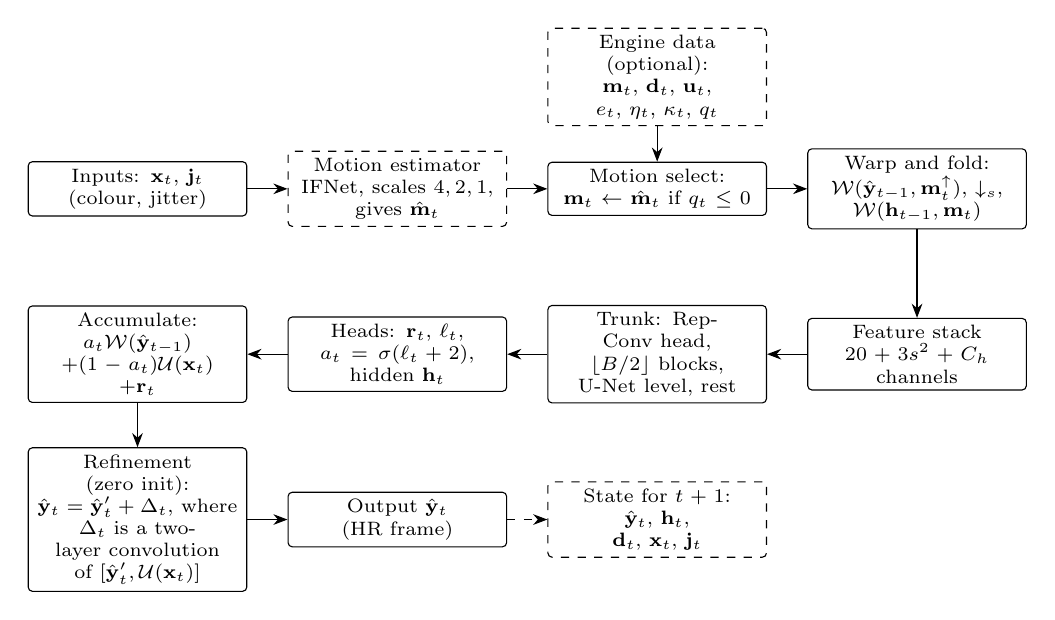
\begin{tikzpicture}[font=\scriptsize, node distance=0pt,
  box/.style={draw, rounded corners=1.5pt, align=center, text width=2.6cm, inner sep=2.5pt},
  opt/.style={box, dashed},
  arr/.style={-{Stealth[length=1.8mm]}},
  rec/.style={-{Stealth[length=1.8mm]}, dashed}]
\node[box] (in) at (0,6.0) {Inputs: $\mathbf{x}_t$, $\mathbf{j}_t$\\(colour, jitter)};
\node[opt] (est) at (3.3,6.0) {Motion estimator\\IFNet, scales $4,2,1$,\\gives $\hat{\mathbf{m}}_t$};
\node[box] (sel) at (6.6,6.0) {Motion select:\\$\mathbf{m}_t\leftarrow\hat{\mathbf{m}}_t$ if $q_t\le 0$};
\node[box] (warp) at (9.9,6.0) {Warp and fold:\\$\mathcal{W}(\hat{\mathbf{y}}_{t-1},\mathbf{m}_t^{\uparrow})$, $\downarrow_s$,\\$\mathcal{W}(\mathbf{h}_{t-1},\mathbf{m}_t)$};
\node[opt, above=0.45cm of sel] (eng) {Engine data (optional):\\$\mathbf{m}_t$, $\mathbf{d}_t$, $\mathbf{u}_t$,\\$e_t$, $\eta_t$, $\kappa_t$, $q_t$};
\node[box] (stack) at (9.9,3.9) {Feature stack\\$20+3s^2+C_h$ channels};
\node[box] (trunk) at (6.6,3.9) {Trunk: RepConv head,\\$\lfloor B/2\rfloor$ blocks,\\U-Net level, rest};
\node[box] (heads) at (3.3,3.9) {Heads: $\mathbf{r}_t$, $\ell_t$,\\$a_t=\sigma(\ell_t+2)$,\\hidden $\mathbf{h}_t$};
\node[box] (acc) at (0,3.9) {Accumulate:\\$a_t\mathcal{W}(\hat{\mathbf{y}}_{t-1})$\\$+(1-a_t)\mathcal{U}(\mathbf{x}_t)$\\$+\mathbf{r}_t$};
\node[box] (refine) at (0,1.8) {Refinement (zero init):\\$\hat{\mathbf{y}}_t=\hat{\mathbf{y}}'_t+\Delta_t$, where\\$\Delta_t$ is a two-layer convolution\\of $[\hat{\mathbf{y}}'_t,\mathcal{U}(\mathbf{x}_t)]$};
\node[box] (out) at (3.3,1.8) {Output $\hat{\mathbf{y}}_t$\\(HR frame)};
\node[opt] (state) at (6.6,1.8) {State for $t+1$:\\$\hat{\mathbf{y}}_t$, $\mathbf{h}_t$,\\$\mathbf{d}_t$, $\mathbf{x}_t$, $\mathbf{j}_t$};
\draw[arr] (in) -- (est);
\draw[arr] (est) -- (sel);
\draw[arr] (sel) -- (warp);
\draw[arr] (eng) -- (sel);
\draw[arr] (warp) -- (stack);
\draw[arr] (stack) -- (trunk);
\draw[arr] (trunk) -- (heads);
\draw[arr] (heads) -- (acc);
\draw[arr] (acc) -- (refine);
\draw[arr] (refine) -- (out);
\draw[rec] (out) -- (state);
\end{tikzpicture}
\caption{Data flow of one TSR time step at scale $s$. Dashed boxes are optional: the engine data are used when the caller supplies them, and the estimator runs in training for every frame and at inference only when a sample has no motion. The state of frame $t$ holds the history, hidden state, depth, colour and jitter that the warp and disocclusion cue of frame $t+1$ read (\cref{sec:tsrm-state})}\label{fig:tsrm-arch}
\end{figure}

\FloatBarrier

\subsection{Inputs}\label{sec:tsrm-inputs}

The trunk receives a stack of channels at render resolution. \Cref{tab:tsrm-inputs} lists them in the order of the code. Seventeen channels come from the frame and its side information, $3s^2$ from the folded history, three from the history disagreement and $C_h$ from the hidden state, so the stack has $20+3s^2+C_h$ channels. For $s=3$ and $C_h=8$ this is $55$, which the code confirms for the \tier{low} tier. The table gives the value that the network sees in each mode. Two replacements happen before the stack is built. A sample without motion receives the estimate $\hat{\mathbf{m}}_t$ and the flag $0.25$ (\cref{sec:tsrm-motion}). A sample with withheld depth receives zero depth and $\eta_t=0$.

The engine motion of the table is the motion in the input, which is exact (synthetic, TartanAir and Sintel), RAFT (real video and GameIR), or absent. The value $\tfrac12$ marks RAFT motion and video samples that keep their motion labels, which are capped at $\tfrac12$ by the degradation of \cref{sec:tsrm-data}.

The depth normalisation of \cref{tab:tsrm-inputs} is
\begin{equation}\label{eq:tsrm-depth}
\mathbf{d}_t=\frac{1}{1+\mathbf{d}^{\mathrm{raw}}_t/\operatorname{med}(\mathbf{d}^{\mathrm{raw}})},
\end{equation}
where $\mathbf{d}^{\mathrm{raw}}$ is the depth in the unit of its source, and $\operatorname{med}$ is the median over the whole sequence for synthetic samples, and over one frame for real windows and test clips. Non-positive and non-finite depth values are set to infinity before the normalisation, so they map to values near zero.

The normals are derived from the normalised depth with edge replication at the border, using the central differences $g^x_t(X,Y)=8\,[\mathbf{d}_t(X+1,Y)-\mathbf{d}_t(X-1,Y)]$ and $g^y_t$ defined in the same way along $Y$:
\begin{equation}\label{eq:tsrm-normal}
\mathbf{n}_t=\eta_t\,\frac{(-g^x_t,\,-g^y_t,\,1)}{\sqrt{(g^x_t)^2+(g^y_t)^2+1}}.
\end{equation}
The factor $8$ is a fixed constant of the code that scales the depth gradient, and the vector is normalised to unit length.

The disocclusion cue compares the current depth with the depth of the previous frame warped to the current frame, using the motion of the network:
\begin{equation}\label{eq:tsrm-disocc}
\delta_t=\eta_t\,\min\Big\{1,\ \frac{\lvert\mathbf{d}_t-\mathcal{W}(\mathbf{d}_{t-1},\mathbf{m}_t)\rvert}{\lvert\mathbf{d}_t\rvert+10^{-3}}\Big\}.
\end{equation}
A large value marks a depth that differs from the warped previous depth, which is typical of a disocclusion. It is a heuristic that the trunk refines, not a visibility test.

\subsection{Motion estimator}\label{sec:tsrm-motion}

The estimator is the IFNet of RIFE 4.26 \cite{huang2022rife} in a narrower form, a coarse-to-fine chain of flow blocks. It is built by \texttt{IFNet(widths, n\_res, n\_hint=3)} in \texttt{nss\_models.py}. Its widths and residual counts are set per tier in the constant \texttt{TSR\_TIERS}: $(32,24,16)$ with two residual blocks for \tier{igpu}, $(48,32,24)$ with three for \tier{low}, $(64,48,32)$ with four for \tier{mid}, $(96,64,48)$ with four for \tier{high}, and $(128,96,64)$ with six for \tier{teacher}. The three levels run at scales $\sigma_1=4$, $\sigma_2=2$ and $\sigma_3=1$ relative to the LR frame, so the coarsest block sees a frame of a quarter of the LR size in each direction.

The estimator takes the previous colour frame $\mathbf{x}_{t-1}$ and the current frame $\mathbf{x}_t$, both padded at the right and bottom by edge replication to multiples of $16$. Its timestep is the constant $1$, so its target frame is the current frame and its reference is the previous one. Its final flow, the first two of its four channels, is the motion of \cref{sec:tsrm-problem}:
\begin{equation}\label{eq:tsrm-est}
\hat{\mathbf{m}}_t=\mathbf{F}^{(3)}_{0},\qquad \mathbf{F}^{(1)}=\Delta^{(1)},\qquad \mathbf{F}^{(k)}=\mathbf{F}^{(k-1)}+\Delta^{(k)}\ \ (k=2,3),
\end{equation}
where $\Delta^{(k)}$ is the four-channel flow update of block $k$ and $\mathbf{F}^{(k)}=(\mathbf{F}^{(k)}_0,\mathbf{F}^{(k)}_1)$ holds the flows from the target to the previous and to the current frame. The flow outputs are multiplied by the block scale, so the flows stay in LR pixels.

The first block receives $\mathbf{x}_{t-1}$, $\mathbf{x}_t$, the per-frame features of both frames and the constant timestep, which is $15$ channels. Each later block receives the colour of both frames warped by the current flow, the features of both frames warped by the current flow, the timestep, the blend mask and the features of the previous block, and the current flow itself, which is $28$ channels. Three hint channels follow for the TSR estimator: the jitter difference $\mathbf{j}_t-\mathbf{j}_{t-1}$ (two channels) and the input kind $\kappa_t$ (one channel). The per-frame feature encoder has a stride-two $3\times3$ convolution and two $3\times3$ convolutions, each followed by LeakyReLU, and a transposed convolution that returns to full resolution with four channels. Inside each block, two stride-two $3\times3$ convolutions reduce the resolution by four, a set of residual $3\times3$ convolutions with a learned per-channel scale follows, and a transposed convolution with pixel shuffle returns to the block resolution with $4$ flow channels, one mask logit and $8$ features.

The estimator is initialised from the RIFE 4.26 weights wherever the names match, and its narrower layers take the leading channel slices of the RIFE tensors. The weight loader \texttt{load\_ifnet\_weights} copies the matching tensors whole and the narrower ones as slices, and the hint channels keep their zero weights. The training log of the \tier{low} run records the result as 11 whole tensors and 42 sliced tensors with no missing tensor. Without the RIFE weights, the code falls back to random initialisation and logs the fact.

The estimate replaces the motion only where the caller gave none. The rule is the one line of \texttt{TSRNet.forward}:
\begin{equation}\label{eq:tsrm-select}
\mathbf{m}_t=\begin{cases}\bar{\mathbf{m}}_t\ \text{(teacher-forced label)} & \text{if } q_t\le 0 \text{ and the sample is forced},\\ \hat{\mathbf{m}}_t & \text{if } q_t\le 0 \text{ otherwise},\\ \text{given motion} & \text{if } q_t>0,\end{cases}
\end{equation}
and the quality flag of every sample with $q_t\le 0$ becomes $\tfrac14$ (the constant \texttt{EST\_MV\_QUALITY}). The flag is therefore the same for estimated and forced samples, and the network cannot tell them apart. At inference the estimator runs only when some sample of the batch has $q_t\le 0$. In training it runs for every frame of every sample, because the motion loss of \cref{sec:tsrm-loss} supervises every sample that has a label, including those with engine motion.

Teacher forcing protects the trunk while the estimator is still poor. A sample without motion is forced to warp its history with the label motion $\bar{\mathbf{m}}_t$ with probability $\pi(\tau)$, drawn once per sample and used for all its frames, where $\tau$ is the elapsed training time and $T_b$ the training budget in seconds:
\begin{equation}\label{eq:tsrm-teacher}
\pi(\tau)=\max\Big(0,\ 1-\frac{\tau}{\rho\,T_b}\Big),\qquad \rho=\Res{tsr.config.cfg.mv_warmup_frac}.
\end{equation}
The forcing applies only to samples that have a label, so $\lambda>0$. Its probability falls linearly from one to zero over the first quarter of the budget, after which no forced mask is drawn. The clock is the wall-clock time of each process from its first step, so the two DDP ranks draw their masks on their own clocks. Teacher forcing is the name for feeding a recurrent predictor a target in place of its own output during training. Here it is this code's schedule, which replaces the estimate by the label for part of the early training only.

\subsection{Warping, folding and the recurrent state}\label{sec:tsrm-state}

The state carried from frame $t-1$ to frame $t$ is
\begin{equation}\label{eq:tsrm-state}
\mathcal{S}_{t-1}=\big(\hat{\mathbf{y}}_{t-1},\ \mathbf{h}_{t-1},\ \mathbf{d}_{t-1},\ \mathbf{x}_{t-1},\ \mathbf{j}_{t-1}\big).
\end{equation}
The depth, colour and jitter are kept for the disocclusion cue and for the estimator of frame $t$. The ONNX export passes them as explicit inputs (\cref{sec:tsrm-deploy}).

The previous output is warped to the HR grid with the upsampled motion. The LR motion is interpolated bilinearly to HR and multiplied by the scale, because a displacement of $d$ LR pixels is $sd$ HR pixels:
\begin{equation}\label{eq:tsrm-up-motion}
\mathbf{m}_t^{\uparrow}=s\cdot\mathrm{Bil}^{\times s}[\mathbf{m}_t],\qquad \mathbf{H}_t=\mathcal{W}\big(\hat{\mathbf{y}}_{t-1},\mathbf{m}_t^{\uparrow}\big),
\end{equation}
where $\mathrm{Bil}^{\times s}$ is bilinear upsampling by $s$ with align-corners set to false. The folded history is $\downarrow_s\mathbf{H}_t\in\mathbb{R}^{3s^2\times h\times w}$, the space-to-depth rearrangement of PyTorch's pixel unshuffle, which places every $s\times s$ block of HR pixels in the channels of one LR pixel. The history disagreement uses the mean of each block, $\bar{\mathbf{H}}_t=\operatorname{avgpool}_s(\mathbf{H}_t)$, and its absolute difference to the LR colour, $\mathbf{g}_t=\lvert\bar{\mathbf{H}}_t-\mathbf{x}_t\rvert$.

The hidden state and the depth are warped at LR with the LR motion $\mathbf{m}_t$, which is the motion of the network. The hidden state after frame $t$ is produced by the trunk, as \cref{sec:tsrm-output} gives. Warping uses the backward warp of \cref{eq:tsrm-warp}:
\begin{equation}\label{eq:tsrm-warp}
\mathcal{W}(I,\mathbf{m})(\mathbf{p})=I\big(\mathbf{p}+\mathbf{m}(\mathbf{p})\big),
\end{equation}
where $I$ is read bilinearly and clamped to its border. The implementation uses grid sampling with align-corners set to true, the convention of RIFE, so that the pixel centres of the first and last rows and columns lie on the image border.

On the first frame of a sequence, or in every frame of the no-history ablation, the state is empty. The history $\mathbf{H}_t$, the folded history, the history disagreement and the warped hidden state are all multiplied by zero, the disocclusion cue is computed against the current depth so that it is zero, and the history weight is set to zero exactly, not learned, by the rule
\begin{equation}\label{eq:tsrm-reset}
a_t=0\quad\text{when the state is empty.}
\end{equation}
The network has no other reset. It has no scene-cut detector, so the history weight must reject a cut by itself. The synthetic renderer produces no cuts, and the cache builders contain no cut filter, so a real window may contain a cut, and the training does not measure how often that happens.

\subsection{Reconstruction trunk}\label{sec:tsrm-trunk}

The trunk is a chain of re-parameterisable blocks, called RepConv here, in the sense of RepVGG \cite{ding2021repvgg} and ECBSR \cite{zhang2021ecbsr}. A RepConv block is trained as a sum of linear branches and deployed as one $3\times3$ convolution. A training forward pass folds the branches into one kernel on every call, so each block costs one convolution in training and one in deployment. The folded kernel for an output channel $o$ and an input channel $i$ is
\begin{equation}\label{eq:tsrm-fold}
\mathbf{W}_{oi}=\mathbf{W}^{(3)}_{oi}+\operatorname{pad}_{3\times3}\big(\mathbf{W}^{(1)}_{oi}\big)+\sum_{k=1}^{3}\mathbf{P}_{o,i,k}\,\mathbf{E}_k+\delta_{oi}\,\mathbf{C},
\end{equation}
with the bias $b_o=b^{(3)}_o+b^{(1)}_o+b^{(e)}_o$. The symbols are as follows. $\mathbf{W}^{(3)}$ is a learned $3\times3$ kernel and $\mathbf{W}^{(1)}$ a learned $1\times1$ kernel, padded with zeros to $3\times3$. The matrices $\mathbf{E}_1$, $\mathbf{E}_2$ and $\mathbf{E}_3$ are the fixed Sobel-x, Sobel-y and Laplacian kernels, $[[-1,0,1],[-2,0,2],[-1,0,1]]$, $[[-1,-2,-1],[0,0,0],[1,2,1]]$ and $[[0,1,0],[1,-4,1],[0,1,0]]$. The coefficients $\mathbf{P}_{o,i,k}$ form a learned $1\times1$ convolution from $3C_i$ inputs to $C_o$ outputs, reshaped so that each input channel $i$ has its three edge responses $k$. The matrix $\mathbf{C}$ has a one at its centre and zeros elsewhere, and the term with $\delta_{oi}$ is present only when $C_i=C_o$. Because the folding is linear, the folded convolution computes exactly the same function as the training branches.

Each RepConv is followed by a PReLU with one learned slope per output channel, initialised to PyTorch's default of $0.25$. The side branches start at zero, in the following sense. The weights of the $1\times1$ branch and of the edge branch are set to zero, so the block starts as a $3\times3$ convolution plus identity. Their biases keep PyTorch's default uniform initialisation, so the side branches do not start exactly at zero. The code records that default initialisation grew the activations by about $1.9$ times per block and gave a non-finite teacher loss from step $10$ in an earlier run \Observation.

The trunk of \cref{eq:tsrm-trunk-def} is built from the stack $\mathbf{z}_t$, which has $20+3s^2+C_h$ channels. Let $\mathrm{RC}_{\mathrm{head}}$ denote the head RepConv block, $\mathcal{A}$ the first $\lfloor B/2\rfloor$ blocks, $\mathcal{B}$ the remaining $B-\lfloor B/2\rfloor$ blocks, and $\mathcal{V}$ the U-Net level, which exists when $U>0$:
\begin{align}
\mathbf{z}_0&=\mathrm{RC}_{\mathrm{head}}(\mathbf{z}_t) \label{eq:tsrm-trunk-def}\\
\mathbf{z}_1&=\mathcal{A}(\mathbf{z}_0)\nonumber\\
\mathbf{z}_2&=\mathbf{z}_1+\mathcal{V}(\mathbf{z}_1)\nonumber\\
\mathbf{y}_t&=\mathcal{B}(\mathbf{z}_2).\nonumber
\end{align}
The head is one RepConv from $20+3s^2+C_h$ channels to $C$ channels. The U-Net level, when present, is a $3\times3$ convolution with stride two from $C$ to $2C$ channels followed by PReLU, then $U$ RepConv blocks at $2C$ channels, then a $1\times1$ convolution from $2C$ to $4C$ channels and a pixel shuffle with factor two, which returns $C$ channels at LR resolution. The U-Net level therefore works at half the LR resolution and is added to the trunk as a residual. The LR input is padded to an even size by edge replication before the trunk, which the stride-two convolution needs. The numbers of blocks per tier are in \cref{tab:tsrm-tiers}.

\subsection{Output head and accumulation}\label{sec:tsrm-output}

The output head is one $3\times3$ convolution from $C$ to $4s^2$ channels, with zero weights and zero bias, applied to $\mathbf{y}_t$. A pixel shuffle with factor $s$ \cite{shi2016espcn} then gives four channels at HR. The first three are the residual $\mathbf{r}_t$ and the fourth is a logit $\ell_t$, and the history weight is
\begin{equation}\label{eq:tsrm-alpha}
a_t=\sigma(\ell_t+2),\qquad \sigma(z)=\frac{1}{1+e^{-z}}.
\end{equation}
At initialisation the zero weights give $\ell_t=0$, so $a_t=\sigma(2)\approx0.881$ and $\mathbf{r}_t=0$, and the network starts as a blend of the warped history and the upsampled colour. The hidden state is produced by a $3\times3$ convolution from $C$ to $C_h$ channels followed by $\tanh$, $\mathbf{h}_t=\tanh(\mathrm{Conv}_{3\times3}(\mathbf{y}_t))$, and it is warped at the next frame by \cref{eq:tsrm-warp}.

The output is the accumulation rule
\begin{equation}\label{eq:tsrm-acc}
\hat{\mathbf{y}}'_t=a_t\odot\mathcal{W}\big(\hat{\mathbf{y}}_{t-1},\mathbf{m}_t^{\uparrow}\big)+(1-a_t)\odot\mathcal{U}(\mathbf{x}_t)+\mathbf{r}_t,
\end{equation}
where $\odot$ is the element-wise product, $\mathcal{U}$ is the jitter-aware bilinear upsampling
\begin{equation}\label{eq:tsrm-up}
\mathcal{U}(\mathbf{x}_t)(X,Y)=\operatorname{Bil}[\mathbf{x}_t]\Big(\frac{X+\tfrac12}{s}-\mathbf{j}_t\Big),
\end{equation}
and $\operatorname{Bil}[\mathbf{x}]$ is the bilinear interpolant of the LR samples, sample $i$ at coordinate $i+\tfrac12$, with clamped borders. The term $\frac{X+1/2}{s}$ is the continuous LR coordinate of output pixel $(X,Y)$, and subtracting $\mathbf{j}_t$ reads each LR sample at its jittered position. The output is then refined as \cref{sec:tsrm-refine} gives. On the first frame, $a_t=0$ by \cref{eq:tsrm-reset}, so $\hat{\mathbf{y}}_0=\mathcal{U}(\mathbf{x}_0)+\mathbf{r}_0$.

\paragraph{Why this is a learned temporal accumulation.} Ignore the residual and the motion for a moment, and let $a_t=a$ be constant, with $\mathbf{m}_t=0$ on a static scene. Then \cref{eq:tsrm-acc} unrolls to
\begin{equation}\label{eq:tsrm-unroll}
\hat{\mathbf{y}}_t=a^{t}\,\mathcal{U}(\mathbf{x}_0)+\sum_{k=1}^{t}(1-a)\,a^{t-k}\,\mathcal{U}(\mathbf{x}_k).
\end{equation}
The weights add to one, because $a^t+(1-a)\sum_{j=0}^{t-1}a^j=a^t+(1-a^t)=1$. The sample $k$ frames old has weight $(1-a)a^{k}$, which is an exponential moving average over the frames of the sequence, with mean age $a/(1-a)$ frames. Each $\mathcal{U}(\mathbf{x}_k)$ reads the colour at a different sub-pixel jitter, so the average gathers the samples of several sub-pixel positions. This is the principle of temporal accumulation for supersampling \cite{yang2020taasurvey} (\cref{sec:bg-taa}). At the initial history weight $\sigma(2)$ the mean age is about $7.4$ frames.

Classical TAA has the same update with a fixed or heuristic blend weight, and it rectifies the reprojected history by clamping it to the colour neighbourhood of the current frame. \Cref{eq:tsrm-acc} keeps the update and changes the rectification. The weight $a_t$ is a learned per-pixel gate, and the network has the disagreement $\mathbf{g}_t$ as input and a receptive field of several convolutions, so the gate can learn to go to zero where the history is invalid, which happens at disocclusions and at particle effects. The residual $\mathbf{r}_t$ corrects the result additively. There is no explicit clamp anywhere in the TSR network, so the residual can move a pixel outside the neighbourhood of the current frame. The analytic baseline of \cref{sec:tsrm-test} does clamp, and the two rectifications are different.

\subsection{Refinement and the reset rule}\label{sec:tsrm-refine}

Every tier except \tier{igpu} refines the accumulated output at HR resolution. The refinement is
\begin{equation}\label{eq:tsrm-refine}
\hat{\mathbf{y}}_t=\hat{\mathbf{y}}'_t+\mathrm{Conv}_{3\times3}\Big(\mathrm{PReLU}\big(\mathrm{Conv}_{3\times3}([\hat{\mathbf{y}}'_t,\mathcal{U}(\mathbf{x}_t)])\big)\Big),
\end{equation}
where $[\cdot,\cdot]$ concatenates six channels. The first convolution has $R$ output channels and the second has three. The second convolution has zero weights and zero bias, so the refinement starts at the identity. Its purpose is to remove the pixel-shuffle pattern of the LR head, as the code comment states. The width $R$ is $8$ for \tier{low} and \tier{mid}, $12$ for \tier{high} and $16$ for the teacher, and the \tier{igpu} tier has no refinement.

The reset rule is \cref{eq:tsrm-reset}. It applies to the first frame of each training window and each test clip, and in every frame of the no-history ablation (\cref{sec:tsrm-abl}). The ONNX step of \cref{sec:tsrm-deploy} has no reset input.

\subsection{Model tiers}\label{sec:tsrm-tiers}

The tiers are the entries of \texttt{TSR\_TIERS} in \texttt{nss\_models.py}. \Cref{tab:tsrm-tiers} gives their widths, block counts, U-Net blocks, hidden widths, estimator, refinement width, parameter counts and costs. The parameter counts are those of the fused network, with the estimator included, and the estimator parameters are the difference from the same network built without the estimator. The costs count multiply-accumulates of every convolution, including the estimator, for one steady-state frame with history, per 1080p output frame, and exclude the warps and the pixel shuffles, which have no multiply-accumulates. The counting is done with forward hooks on the fused network in \texttt{tsr\_macs\_per\_lr\_pixel}, and the notebook scales it by the LR pixel count.

The fused parameter counts and the 3x and 2x costs are the values that \texttt{model\_tiers.csv} records for the run. They were also recomputed from \texttt{src/neuralss/nss\_models.py} on the current code, and both agree. The estimator column is the difference between the training parameter count with and without the estimator, which is also computed from the code. The \tier{mid} and \tier{high} tiers are defined and costed, but the TSR notebook never trains them. Its runs use the teacher at 3x, \tier{low} at 3x and 2x, \tier{igpu} at 3x, and the six ablation runs at 3x, which all use \tier{low}. The tier table of the article (\cref{M-tab:tiers}) therefore gives no latency for these two tiers.

The estimator holds a large share of the training parameters of every tier. It is about $81$ percent for \tier{igpu}, $63$ percent for \tier{low} and $51$ percent for the teacher, and it runs on every frame without engine motion.

\subsection{Training samples and degradations}\label{sec:tsrm-data}

Each training step draws from two streams, and both produce sequences of $T$ frames with HR targets, LR inputs, motion labels and validity masks. The synthetic stream renders layered game-like scenes from cached texture crops with the renderer of \cref{sec:data-synth}. Its scene parameters, which are used here, are a background layer and a foreground layer with procedural alpha (a superellipse, four thin wires each present with probability $0.6$, and a fence present with probability $0.35$), moving on continuous affine paths. The foreground texture is flat with probability $0.25$ and is otherwise the still of the neighbouring sample in the batch, the foreground layer is present with probability $0.85$, world-space text tiles are stamped into the background with probability $0.3$, and six particles are drawn, each active with probability $0.5$. The motion class is static, slow, medium or fast with probabilities $0.15$, $0.45$, $0.25$ and $0.15$, which give speeds of $0$, $0.3$ to $3$, $3$ to $10$ and $10$ to $28$ output pixels per frame. Each sample has an exposure $2^{u}$ with $u$ uniform on $[-0.8,0.8]$, and a sub-pixel jitter phase drawn uniformly from the sixteen Halton offsets. The LR frames are single-sample jittered reads of the renderer, and the HR targets are four-sample renders.

The real stream reads cached windows of $T$ frames at $P=192$ output pixels from the sequence sources of \cref{sec:data}. The window is drawn from a source-specific downscale range before cropping. A real window is flipped horizontally with probability $\tfrac12$ and vertically with probability $\tfrac12$, and its motion vectors are negated in the flipped components. It is scaled in linear light by an exposure gain $2^{u}$ with $u$ uniform on $[-0.8,0.8]$. Its LR frames are jittered bilinear reads of the HR frame, so they are aliased like a render. The labels are the cached motion and validity, with the label quality of the window. Exact motion, from TartanAir and Sintel, has label quality $1$. Other windows get RAFT motion when RAFT is available, with label quality $\tfrac12$, and otherwise zero motion with label quality $0$. \Cref{tab:tsrm-mix} lists the probabilities that the TSR configuration or the degradation functions set.

\begin{table}[!htbp]
\caption{Probabilities of the TSR training data that are set by the TSR configuration or by the degradation functions. The renderer's own probabilities are given in \cref{sec:tsrm-data} and \cref{sec:data-synth}}\label{tab:tsrm-mix}
{\scriptsize\raggedright\setlength{\tabcolsep}{3pt}
\begin{tabular*}{\textwidth}{@{\extracolsep\fill}p{0.44\textwidth}p{0.16\textwidth}p{0.32\textwidth}}
\toprule
Quantity & Value & Code location \\
\midrule
Real windows per batch & $\Res{tsr.config.cfg.p_real}$, so $19$ of $48$ & \texttt{p\_real}, \texttt{make\_loader} \\
Synthetic samples turned into plain video & $\Res{tsr.config.cfg.p_video_synth}$ & \texttt{p\_video\_synth}, \texttt{video\_degrade} \\
Real samples turned into plain video & $\Res{tsr.config.cfg.p_video_real}$ & \texttt{p\_video\_real}, \texttt{video\_degrade} \\
Plain-video samples that keep their motion labels & $\Res{tsr.config.cfg.p_video_mv}$ & \texttt{p\_video\_mv}, \texttt{video\_degrade} \\
Samples that lose their motion vectors (all samples of the batch) & $\Res{tsr.config.cfg.p_drop_mv}$ & \texttt{p\_drop\_mv}, \texttt{withhold\_engine\_data} \\
Samples that lose their depth (all samples of the batch) & $\Res{tsr.config.cfg.p_drop_depth}$ & \texttt{p\_drop\_depth}, \texttt{withhold\_engine\_data} \\
Long steps, every fourth step from step $0$ & $1/\Res{tsr.config.cfg.long_every}$ & \texttt{long\_every} $=\Res{tsr.config.cfg.long_every}$, \texttt{train\_tsr.step\_fn} \\
Teacher forcing of motion & $\pi(\tau)$ in \cref{eq:tsrm-teacher} & \texttt{mv\_warmup\_frac} $=\Res{tsr.config.cfg.mv_warmup_frac}$ \\
Horizontal and vertical flip of real windows & $1/2$ each & \texttt{sr\_batch\_from\_frames} \\
Gain of real windows and scene exposure & $2^{u}$, $u\sim U[-0.8,0.8]$ & \texttt{sr\_batch\_from\_frames}, \texttt{Scene} \\
Downscale filter of plain video (bicubic, bilinear, box) & $1/3$ each & \texttt{video\_lr} \\
Blur $\sigma$ of plain video & $U[0,0.6]$ output pixels & \texttt{video\_lr} \\
Noise $\sigma$ of plain video & $U[0,2/255]$ & \texttt{video\_lr} \\
\botrule
\end{tabular*}}
\end{table}

The plain-video degradation turns a sample into ordinary video. A plain-video LR frame is the target frame $\mathbf{y}$ after a Gaussian blur, an anti-aliased downscale, additive noise and 8-bit quantisation. The blur is a five-tap separable Gaussian on the output grid with $\sigma$ uniform on $[0,0.6]$. The downscale $D$ is bicubic (cubic convolution \cite{keys1981bicubic}), bilinear or box averaging, each chosen with probability $1/3$. The noise is added after the downscale, with $\sigma_n$ uniform on $[0,2/255]$, and the frame is clamped and rounded to multiples of $1/255$:
\begin{equation}\label{eq:tsrm-video}
\mathbf{x}^{\mathrm{vid}}_t=\mathrm{round}_{1/255}\Big(\mathrm{clip}_{[0,1]}\big(D\big(G_\sigma\ast\mathbf{y}_t\big)+\mathbf{n}\big)\Big),\qquad \mathbf{n}\sim\mathcal{N}(0,\sigma_n^2 I).
\end{equation}
A plain-video sample loses its jitter, its depth, its reactive mask and its depth availability, and its input kind becomes $\kappa_t=0$. Its motion is removed, except for the share $p_\mathrm{mv}=0.15$ that keeps the label motion with flag $\min(q,\tfrac12)$. The label motion of a plain-video sample is the block mean of the HR motion, divided by $s$, and its validity is one only where all $s\times s$ HR pixels are valid. The labels keep their label quality, so a plain-video sample still supervises the estimator.

The withholding rule is applied to the whole batch after both streams are built. Its two masks are drawn once per sample and apply to every sample, including the plain-video samples that kept their motion. A sample loses its motion with probability $0.25$, and it loses its depth with probability $0.3$. A plain-video sample that kept its motion therefore loses it with probability $0.25$.

Most real windows come from Vimeo-90K \cite{xue2019vimeo}, and only a small share has exact motion, as \cref{M-sec:discussion} reports \UnderRevision. The configuration gives the cache capacities of \Res{tsr.config.cfg.cache.still_train} still crops and \Res{tsr.config.cfg.cache.win_train} windows.

\subsection{Unroll lengths and patch sizes}\label{sec:tsrm-unroll}

Each training window has $T=\Res{tsr.config.cfg.seq_len}$ frames of $P=\Res{tsr.config.cfg.patch}$ output pixels, which is $64$ LR pixels at $s=3$ and $96$ at $s=2$. The network runs through the frames of a window in order, the state starts empty, and the loss of every frame is summed before one backward pass. The gradient flows through every frame of the window, and it stops at the window boundary, which is truncated back-propagation through time \cite{williams1990efficient}. The notebook gives six frames per window, as truncated back-propagation through the recurrence, and 192-pixel patches as its defaults. It sets $\Res{tsr.config.cfg.still_size}$-pixel texture crops so that fast camera paths have room inside the texture.

Every fourth step is a long step with $T=\Res{tsr.config.cfg.long_t}$ frames of $P=\Res{tsr.config.cfg.long_patch}$ pixels, which is $16\times96^2=147{,}456$ output pixels per window, two thirds of the $6\times192^2=221{,}184$ of a normal window. The notebook gives the reason for the long steps as the decline of the earlier students on static scenes after frames $6$ to $10$, which the notebook measured in one earlier run \Preliminary. The long steps use only synthetic windows, so each GPU has $48-19=29$ of them in a long step, against $48$ windows in a normal step.

The batch is $48$ windows per GPU for the teacher and for the students. The batch probe of the notebook tried sizes $4$, $8$, $12$, $16$, $24$, $32$ and $48$, and it kept the largest size that stayed below $75$ percent of GPU memory. Both models passed at $48$ with memory use well below that limit, so the list, not the memory, set the batch. The main stages run on both GPUs with distributed data parallel, which gives $96$ windows per step, and the paired runs and ablations run on one GPU each, with $48$ windows per step.

\subsection{Loss}\label{sec:tsrm-loss}

The loss is computed for every window and then averaged over the batch. For the frames $t=0,\dots,T-1$ of a window, let $\hat{\mathbf{y}}_t$ be the output and $\mathbf{y}_t$ the target. The pixel term is a Charbonnier penalty, with $\varepsilon=10^{-3}$, averaged over the frames with weight $\tfrac14$ on the first frame, which has no history:
\begin{equation}\label{eq:tsrm-lpix}
\mathcal{L}_\mathrm{pix}=\frac{\sum_{t}\omega_t\,\mathbb{E}\sqrt{(\hat{\mathbf{y}}_t-\mathbf{y}_t)^2+\varepsilon^2}}{\sum_t\omega_t},\qquad \omega_0=\tfrac14,\ \ \omega_t=1\ \ (t\ge1).
\end{equation}
The expectation $\mathbb{E}$ is the mean over the channels and pixels of the batch. The Charbonnier penalty \cite{charbonnier1997deterministic} is a smooth edge-preserving potential that approximates the absolute difference.

The gradient term compares the finite differences of the output and the target over a distance of two pixels in each direction. With $D_x\mathbf{z}(X,Y)=\mathbf{z}(X+2,Y)-\mathbf{z}(X,Y)$ and $D_y$ defined in the same way along $Y$,
\begin{equation}\label{eq:tsrm-lgrad}
\mathcal{L}_\mathrm{grad}=\mathbb{E}_t\big|D_x\hat{\mathbf{y}}_t-D_x\mathbf{y}_t\big|+\mathbb{E}_t\big|D_y\hat{\mathbf{y}}_t-D_y\mathbf{y}_t\big|,
\end{equation}
where $\mathbb{E}_t$ is the mean over all frames of the window, the channels and the pixels.

The Fourier term compares the magnitudes of the two-dimensional spectra of the frames, computed with the orthonormal real FFT, so that texture energy at every frequency counts:
\begin{equation}\label{eq:tsrm-lfft}
\mathcal{L}_\mathrm{fft}=\mathbb{E}_t\Big|\,\big|\mathcal{F}\hat{\mathbf{y}}_t\big|-\big|\mathcal{F}\mathbf{y}_t\big|\,\Big|,
\end{equation}
where $\mathcal{F}$ is the orthonormal real two-dimensional FFT of each channel and $|\cdot|$ is the complex magnitude.

The temporal term matches the change of the output to the change of the target along the label motion, at HR, over the pixels that are visible in both frames:
\begin{multline}\label{eq:tsrm-ltmp}
\mathcal{L}_\mathrm{tmp}=\frac{1}{T-1}\sum_{t=1}^{T-1}\frac{\sum_{\mathbf{p}}\bar{\mathbf{V}}_t(\mathbf{p})\,\lambda_t\sum_{c}\big|\Delta^{\mathrm{out}}_{t,c}(\mathbf{p})-\Delta^{\mathrm{gt}}_{t,c}(\mathbf{p})\big|}{3\sum_{\mathbf{p}}\bar{\mathbf{V}}_t(\mathbf{p})\,\lambda_t+10^{-6}},
\end{multline}
where $\Delta^{\mathrm{out}}_t=\hat{\mathbf{y}}_t-\mathcal{W}(\hat{\mathbf{y}}_{t-1},\bar{\mathbf{M}}_t)$ and $\Delta^{\mathrm{gt}}_t=\mathbf{y}_t-\mathcal{W}(\mathbf{y}_{t-1},\bar{\mathbf{M}}_t)$ are the temporal changes of the output and of the target along the label motion, $\bar{\mathbf{M}}_t$ is the HR label motion, $\bar{\mathbf{V}}_t$ its validity and $\lambda_t$ its label quality. The term is zero for windows without labels.

The motion term supervises the estimator on every frame after the first, with the LR label motion $\bar{\mathbf{m}}_t$ and its validity $\bar{\mathbf{v}}_t$:
\begin{equation}\label{eq:tsrm-lflow}
\mathcal{L}_\mathrm{flow}=\frac{\sum_{t=1}^{T-1}\sum_{\mathbf{p}}\lambda_t\,\bar{\mathbf{v}}_t(\mathbf{p})\,\big\lVert\hat{\mathbf{m}}_t(\mathbf{p})-\bar{\mathbf{m}}_t(\mathbf{p})\big\rVert_1}{\sum_{t=1}^{T-1}\sum_{\mathbf{p}}\lambda_t\,\bar{\mathbf{v}}_t(\mathbf{p})+1},
\end{equation}
where $\lVert\cdot\rVert_1$ sums the absolute differences of the two components, so the error is measured in LR pixels. The $+1$ in the denominator avoids a division by zero when no window has a valid label.

The perceptual term is LPIPS \cite{zhang2018lpips} with its AlexNet backbone on the last frame of the window, computed on the output clamped to $[0,1]$:
\begin{equation}\label{eq:tsrm-llp}
\mathcal{L}_\mathrm{lp}=\mathbb{E}_{\mathrm{batch}}\,\mathrm{LPIPS}\big(\mathrm{clip}_{[0,1]}(\hat{\mathbf{y}}_{T-1}),\mathbf{y}_{T-1}\big).
\end{equation}
The distillation term $\mathcal{L}_\mathrm{kd}$ is the mean absolute difference between the output and the output of a frozen teacher on the same inputs. It is inactive (\cref{sec:tsrm-distill}). The total loss is
\begin{equation}\label{eq:tsrm-loss}
\mathcal{L}=\mathcal{L}_\mathrm{pix}+\Res{tsr.config.cfg.w_grad}\,\mathcal{L}_\mathrm{grad}+\Res{tsr.config.cfg.w_fft}\,\mathcal{L}_\mathrm{fft}+\Res{tsr.config.cfg.w_temporal}\,\mathcal{L}_\mathrm{tmp}+\Res{tsr.config.cfg.w_flow}\,\mathcal{L}_\mathrm{flow}+\Res{tsr.config.cfg.w_lpips}\,\mathcal{L}_\mathrm{lp}+\Res{tsr.config.cfg.w_distill}\cdot\mathcal{L}_\mathrm{kd}.
\end{equation}
The weights are the configuration values \texttt{w\_grad}, \texttt{w\_fft}, \texttt{w\_temporal}, \texttt{w\_flow}, \texttt{w\_lpips} and \texttt{w\_distill} of the run. The frames that each term uses are stated with its equation, and the validation metric is not part of the loss.

\subsection{Optimisation, schedule, precision, moving average and checkpoints}\label{sec:tsrm-optim}

The optimiser is AdamW \cite{loshchilov2019adamw} with betas $(0.9,\,0.99)$, PyTorch's default $\epsilon=10^{-8}$ and weight decay $\Res{tsr.config.cfg.weight_decay}$, applied to every parameter. The peak learning rate is $\Res{tsr.config.cfg.lr}$ for the students and $\Res{tsr.config.cfg.lr_teacher}$ for the teacher. The learning rate follows the wall-clock budget. Let $\varrho=\tau/T_b$ be the fraction of the budget used, with $\varrho_w=\Res{tsr.config.cfg.warmup_frac}$, $\alpha_0$ the peak learning rate and $\alpha_\mathrm{min}=\Res{tsr.config.cfg.min_lr}$:
\begin{equation}\label{eq:tsrm-lr}
\alpha(\varrho)=\begin{cases}\alpha_0\,\max\big(\varrho/\varrho_w,\ 0.01\big), & \varrho<\varrho_w,\\[2pt] \alpha_\mathrm{min}+\tfrac12(\alpha_0-\alpha_\mathrm{min})\Big(1+\cos\Big(\pi\,\dfrac{\varrho-\varrho_w}{1-\varrho_w}\Big)\Big), & \varrho\ge\varrho_w.\end{cases}
\end{equation}
The first $3$ percent of the budget is a linear warm-up from $0.01\,\alpha_0$, and the rest is a single cosine decay without restarts, the decay used within each cycle of SGDR \cite{loshchilov2017sgdr}. The rate is updated every $10$ steps, together with the decision to stop and the validation check, because the processes agree on the elapsed time only at those points.

The gradients are unscaled and their global $L_2$ norm is clipped to $1$ before the optimiser step. The forward pass of the network and of the teacher, when there is one, runs under FP16 autocast, and the losses are computed in FP32 \cite{micikevicius2018mixed}. A dynamic gradient scaler with PyTorch's default initial scale multiplies the loss before the backward pass, and it skips the step when a gradient is non-finite. A run whose loss stays non-finite for $200$ steps stops with an error, so that a diverged run does not use its whole budget.

The moving average of the weights is the recursion below, which is this work's choice.
\begin{equation}\label{eq:tsrm-ema}
\theta^{\mathrm{EMA}}_k=d_k\,\theta^{\mathrm{EMA}}_{k-1}+(1-d_k)\,\theta_k,\qquad d_k=\min\Big(\Res{tsr.config.cfg.ema_decay},\ \frac{1+k}{10+k}\Big),
\end{equation}
where $k\ge1$ counts the updates of the average on rank $0$. The warm-up rule $\min\big((1+k)/(10+k),\ \mathrm{decay}\big)$ is this code's choice, and it makes the averaging window $1/(1-d_k)=(10+k)/9$ updates at update $k$, until the cap $\Res{tsr.config.cfg.ema_decay}$ is reached at $k\approx8{,}990$ updates. The average is therefore short for most of a run and reaches its full window only late in the run, and the validation and the checkpoints of \cref{sec:tsrm-test} use the averaged weights.

Validation runs every $\min(\Res{tsr.config.cfg.val_interval_min}\text{ min},\ \max(T_b/6,\ 60\text{ s}))$ and once more at the end of the budget. It uses a fixed validation set: the first $32$ still crops and the first $32$ windows of the validation caches, in \Res{tsr.config.cfg.val_batches} batches of $\Res{tsr.config.cfg.val_bs}$ still crops and $\Res{tsr.config.cfg.val_bs}$ windows, each evaluated twice. The render copy keeps the engine data, and the plain-video copy degrades every sample with the probability $1$ of \cref{sec:tsrm-data}. The score is the PSNR on luma (\cref{eq:tsrm-psnr}) over the frames $1$ to $T-1$ of each window, with the $s$-pixel border removed, averaged over the windows of each copy, and the selection score is the mean of the two copies.

Each validation round saves the raw and the averaged weights. The averaged weights of the first round with the highest score are kept separately, and evaluation loads them.

The stage budgets are $\Res{tsr.config.cfg.minutes.teacher}$ minutes for the teacher, $\Res{tsr.config.cfg.minutes.student}$ minutes for the \tier{low} student at $3\times$, $\Res{tsr.config.cfg.minutes.pair}$ minutes for each of the paired \tier{igpu} at $3\times$ and \tier{low} at $2\times$ runs, and $\Res{tsr.config.cfg.minutes.ablation}$ minutes for each ablation. The seeds are the configuration seed $\Res{tsr.config.cfg.seed}$ plus the rank for the model, and $100\times\Res{tsr.config.cfg.seed}$ plus the rank for the generator of the synthetic renderer, which keeps every rank's random streams apart. The data loader draws its windows from memory-mapped caches without replacement inside a batch, and each batch index selects its own random generator seed.

\subsection{Per-frame training loop}\label{sec:tsrm-loop}

The training loop of \texttt{train\_loop} and \texttt{train\_tsr.step\_fn} runs the following steps for every iteration on each rank.

\begin{enumerate}
\item Draw one batch from the memory-mapped caches: $19$ real windows and $29$ synthetic still crops on each GPU in a normal step. The indices are sorted and drawn without replacement within the batch.
\item Decide the step type. A step whose index is a multiple of four is a long step, with $29$ synthetic windows of $16$ frames at $96$ pixels, and the teacher is not run. Otherwise the batch is $6$-frame windows, with the real windows in the batch.
\item Build the synthetic windows with the renderer (\texttt{sr\_batch}): motion class, jitter phase, exposure, particles, text, the LR jittered samples, the HR four-sample targets, the exact motion and validity at LR and HR, depth, and the reactive masks.
\item Build the real windows (\texttt{sr\_batch\_from\_frames}): random flips with the motion components negated, the exposure gain in linear light, jittered bilinear reads of the HR frames, and the cached motion, validity and depth.
\item Degrade the plain-video shares: a synthetic window with probability $0.3$, a real window with probability $0.6$, with the filter, blur and noise of \cref{eq:tsrm-video}. The degraded samples keep their motion labels with probability $0.15$.
\item Withhold the engine data of the batch: motion with probability $0.25$ and depth with probability $0.3$, drawn once per sample.
\item Compute the teacher-forcing probability $\pi(\tau)$ of \cref{eq:tsrm-teacher} from the elapsed time, draw the forced mask for the samples with no motion and a label, and add it to the batch when $\pi>0$.
\item Run the recurrent unroll under FP16 autocast. For each frame $t$ in order: form the inputs of \cref{tab:tsrm-inputs}, run the estimator for every frame in training, select the motion of \cref{eq:tsrm-select}, warp and fold the state, run the trunk and the heads, accumulate with \cref{eq:tsrm-acc}, refine with \cref{eq:tsrm-refine}, and keep the state for the next frame. The first frame starts from the reset state.
\item Compute the losses of \cref{eq:tsrm-lpix,eq:tsrm-lgrad,eq:tsrm-lfft,eq:tsrm-ltmp,eq:tsrm-lflow,eq:tsrm-llp} in FP32 and their weighted sum \cref{eq:tsrm-loss}.
\item Scale the loss, run the backward pass through the whole unroll, unscale the gradients, clip their global norm to $1$, and take one AdamW step. A non-finite gradient skips the step.
\item Update the moving average of the weights on rank $0$ with \cref{eq:tsrm-ema}.
\item Every $10$ steps, all-reduce the elapsed time, the stop flag and the memory counters. Set the learning rate by \cref{eq:tsrm-lr}, count the consecutive non-finite checks, and run the validation of \cref{sec:tsrm-optim} when the interval has passed or the budget has ended. Save the checkpoints and, when the validation score is a new best, the best averaged weights.
\item Stop when the budget is used, write the history of the rounds, and report the best round.
\end{enumerate}

\subsection{Distillation}\label{sec:tsrm-distill}

The training code contains a distillation path. A frozen teacher is unrolled on the same inputs without gradients, and its output enters the loss through \cref{eq:tsrm-loss} with weight $w_\mathrm{distill}$. No TSR run used it, because each run sets the teacher checkpoint to none and the weight to zero. The teacher of the article is therefore trained directly, as the quality ceiling, and not distilled. The earlier runs of 20 to 21 and 24 October 2026 recorded no measurable gain from distillation, which the notebook gives as the reason for switching it off \Preliminary.

\subsection{Ablation configurations}\label{sec:tsrm-abl}

Every ablation trains the \tier{low} tier at $3\times$ for $\Res{tsr.config.cfg.minutes.ablation}$ minutes, two at a time on the two GPUs, against a reference run of the same recipe and budget. \Cref{tab:tsrm-abl-config} lists what each one changes and how the change is implemented. The reference is the full recipe at the same budget.

\begin{table}[!htbp]
\caption{TSR ablation configurations. Each row changes one part of the \tier{low} recipe at $3\times$ and $\Res{tsr.config.cfg.minutes.ablation}$ minutes, against the reference}\label{tab:tsrm-abl-config}
{\scriptsize\raggedright\setlength{\tabcolsep}{3pt}
\begin{tabular*}{\textwidth}{@{\extracolsep\fill}p{0.31\textwidth}p{0.30\textwidth}p{0.31\textwidth}}
\toprule
Name & Change & Implementation \\
\midrule
\texttt{abl\_reference} & None & Full recipe with the same $30$-minute budget \\
\texttt{abl\_no\_history} & Single-frame upscaling: no history, no hidden state & \texttt{use\_history=False}: every frame resets (\cref{eq:tsrm-reset}), and unused parameters are allowed in DDP \\
\texttt{abl\_no\_gbuffers} & Colour-only render input: the estimator supplies the motion & \texttt{ablate\_gbuffers}: depth, motion, depth availability and motion quality are zero in every frame \\
\texttt{abl\_no\_motion\_net} & No motion estimator, colour-only input, zero motion & \texttt{motion\_net=False} and \texttt{ablate\_gbuffers}: no estimator and no motion loss \\
\texttt{abl\_no\_video\_training} & Render-like samples only & Both video shares set to zero, the \texttt{p\_video} keys of the configuration, and the withholding of \cref{sec:tsrm-data} still applies \\
\texttt{abl\_no\_long\_unroll} & Six-frame windows only & \texttt{long\_every}$=0$ \\
\botrule
\end{tabular*}}
\end{table}

Each ablation validates on batches built with its own recipe, so validation scores are not comparable between ablations. The test protocol of \cref{sec:tsrm-test} evaluates them all on the same suites. Its engine-mode evaluation of \texttt{abl\_no\_motion\_net} is an exception. The evaluation sets the colour-only flag only for \texttt{abl\_no\_gbuffers} and the no-history flag only for \texttt{abl\_no\_history}. The engine-mode rows of \texttt{abl\_no\_motion\_net} therefore receive depth and motion that the model was never trained with \UnderRevision. The plain-mode rows of this ablation are not affected, because plain inputs have no engine data, and \cref{M-tab:tsr-abl} uses only those rows.

\subsection{Fusion, precision and export}\label{sec:tsrm-deploy}

Fusion replaces every RepConv by a plain $3\times3$ convolution with the folded kernel and bias of \cref{eq:tsrm-fold}, followed by a copy of its PReLU. The rest of the network is unchanged. The motion estimator is built from ordinary convolutions and is not folded. The fused and unfused networks compute the same function up to floating-point error, and the notebook checks the difference on a synthetic batch of each scale and records the maximum absolute difference in FP32.

The evaluation and the latency measurements use the fused networks converted to FP16 weights, and the evaluation runs them under autocast. The latency is the mean over $100$ timed forward passes of one fused FP16 step at batch $1$, after $10$ warm-up steps, with CUDA events and cuDNN autotuning. It is measured at $1080$p and $2160$p outputs for $3\times$ and at $1080$p for $2\times$. The arithmetic estimate in the notebook is a parameter, not a measurement. All latencies are eager PyTorch on one T4, and in-engine latency on target GPUs is not measured \UnderRevision.

The ONNX export wraps one fused step with explicit state tensors. Its inputs are the colour, depth, motion, reactive mask, exposure, jitter, a flag vector of depth availability, motion quality and input kind, and the previous output, hidden state, depth, colour and jitter. Its outputs are the output and the new hidden state. The export uses opset $17$ with the TorchScript exporter, static shapes for one LR size (the notebook uses $36\times64$ and the scale), and it is checked with ONNX Runtime on the CPU against PyTorch in FP32. A deployment must export one graph per render resolution.

The exported step has no reset input. The caller supplies the previous output for the first frame, and the graph then blends that output with the learned weight $a_t$, instead of the zero weight of \cref{eq:tsrm-reset}. The notebook's export test runs a single frame and does not exercise the first frame of a sequence. An engine integration must therefore supply a valid previous output on the first frame, which the export does not check \UnderRevision.

\subsection{Test protocol}\label{sec:tsrm-test}

The test suites are built from the test split of the manifest, which the notebook loads before the evaluation and never uses for training. \Cref{tab:tsrm-suites} lists them. A clip is the first $T$ frames of an item, starting at frame $0$, cropped at the centre to the crop size of its suite. The first $4n$ items of a source with at least $T$ frames are tried, and a clip is skipped when it cannot be decoded or when one of its frames is blank, meaning a luma standard deviation below $2$ on the $0$ to $255$ scale. A blank frame would be reconstructed exactly by every method and would score the PSNR cap of $100$ dB. Clips with frozen frames or scene cuts are not filtered.

\begin{table}[!htbp]
\caption{TSR test suites. Motion labels are exact (renderer or exact flow) or RAFT. Each suite runs in both modes except GameIR, which runs in engine mode only}\label{tab:tsrm-suites}
{\scriptsize\raggedright\setlength{\tabcolsep}{3pt}
\begin{tabular*}{\textwidth}{@{\extracolsep\fill}p{0.19\textwidth}p{0.37\textwidth}p{0.17\textwidth}p{0.04\textwidth}p{0.12\textwidth}}
\toprule
Suite & Source and frame size & Motion & $T$ & Scales \\
\midrule
\texttt{synthetic-game} & Game stills and DIV2K \cite{agustsson2017div2k} test items, $1024$-pixel texture crops, rendered at $\Res{tsr.config.cfg.eval.synthetic_p}$ output pixels, six sequences per motion class & Exact & $\Res{tsr.config.cfg.eval.synthetic_t}$ & $3\times$, $2\times$ \\
\texttt{tartanair} & TartanAir \cite{wang2020tartanair} test environments, $480\times576$ & Exact (forward flow played backwards) & $\Res{tsr.config.cfg.eval.real_t}$ & $3\times$, $2\times$ \\
\texttt{sintel} & MPI Sintel \cite{butler2012sintel} test scene families, $432\times1008$ & Exact (with occlusion masks) & $\Res{tsr.config.cfg.eval.real_t}$ & $3\times$, $2\times$ \\
\texttt{vid4} & Vid4 \cite{liu2014vid4} test sequences, $480\times696$ & RAFT & $\Res{tsr.config.cfg.eval.real_t}$ & $3\times$, $2\times$ \\
\texttt{vimeo1080p} & Pinned validation shards of Vimeo-1080p, which the manifest assigns to the test split, shorter side at most $540$, crop $540\times960$ & RAFT & $\Res{tsr.config.cfg.eval.real_t}$ & $3\times$, $2\times$ \\
\texttt{gameir-native} & GameIR \cite{zhou2024gameir} test town, $720$p native input and $1440\times1920$ target & RAFT, engine mode only & $6$ & $2\times$ \\
\botrule
\end{tabular*}}
\end{table}

In engine mode the network receives the jittered single-sample input of each suite, with the motion labels as motion vectors and the depth where the source has it. On the real video suites and GameIR the motion is RAFT-small \cite{teed2020raft} with its default weights, run for $12$ iterations on the clean full-resolution frames, and it is kept where the forward-backward error is below one pixel plus five percent of the flow magnitude. RAFT sees the target frames rather than the jittered input, so engine mode on these suites is an oracle for motion, as the notebook notes \UnderRevision. In plain mode the input is the anti-aliased bicubic downscale of the target, and the exact or RAFT motion serves only as a metric label. The synthetic suite uses the same text-tile bank as training, generated with the same seed.

The baselines are jitter-aware bicubic and bilinear upsampling in both modes, the bilinear one being $\mathcal{U}$ of \cref{eq:tsrm-up}, and the analytic TAA upscaler in engine mode only. TAA reprojects its history with the engine motion, clamps the history to the $3\times3$ YCoCg neighbourhood of the current bilinear upsample, and blends in $10$ percent of the new frame. The networks are the teacher, \tier{low} and \tier{igpu} at $3\times$, the \tier{low} student at $2\times$, and the six ablations at $3\times$, in both modes.

The static-convergence test is a separate run. It renders a camera at rest with sub-pixel jitter on the synthetic static class, with the first six test stills, sixteen frames and the seed $4242$, in engine mode. It covers the bilinear and TAA baselines, the \tier{low}, \tier{igpu} and teacher networks, and the reference, no-long-unroll and no-history ablations. Its per-frame PSNR is averaged over the six sequences, and the FLIP error \cite{andersson2020flip} of the last frame is reported.

\subsection{Metrics and aggregation}\label{sec:tsrm-metrics}

The metrics are computed for every frame $t\ge1$ of every clip, because the first frame has no history. The luma of an RGB image $\mathbf{c}\in[0,1]^3$ is the limited-range value
\begin{equation}\label{eq:tsrm-luma}
Y(\mathbf{c})=\frac{16+65.481\,c_R+128.553\,c_G+24.966\,c_B}{255},
\end{equation}
which lies in $[16/255,235/255]$. The peak-signal-to-noise ratio of luma is then
\begin{equation}\label{eq:tsrm-psnr}
\mathrm{PSNR}_Y=10\log_{10}\frac{1}{\mathrm{MSE}},\qquad \mathrm{MSE}=\frac{1}{|\Omega|}\sum_{\mathbf{p}\in\Omega}\big(Y(\hat{\mathbf{y}}_t)(\mathbf{p})-Y(\mathbf{y}_t)(\mathbf{p})\big)^2,
\end{equation}
where $\Omega$ is the set of output pixels with an $s$-pixel border removed on each side. The structural similarity (SSIM) \cite{wang2004ssim} uses the same luma and border with an $11\times11$ Gaussian window of standard deviation $1.5$. The detail PSNR uses the top $15$ percent of the gradient magnitude of the target luma, which contains thin geometry, foliage and text. The disoccluded PSNR and the particle PSNR use the pixels with $\bar{\mathbf{V}}_t=0$ and the pixels where the reactive mask, upsampled by nearest neighbour, exceeds $0.1$, each when the batch holds more than $50$ such pixels. This rule is tested over the whole batch and not per sample, so in a batch of several synthetic samples a sample without such pixels receives the cap of $100$ dB \UnderRevision.

The warping error measures the output alone along the exact label motion, and it is defined for $\lambda_t=1$:
\begin{equation}\label{eq:tsrm-warpe}
E_\mathrm{w}(t)=\frac{\sum_{\mathbf{p}}\bar{\mathbf{V}}_t(\mathbf{p})\,\frac13\sum_c\big|\hat{\mathbf{y}}_t-\mathcal{W}(\hat{\mathbf{y}}_{t-1},\bar{\mathbf{M}}_t)\big|_c(\mathbf{p})}{\sum_{\mathbf{p}}\bar{\mathbf{V}}_t(\mathbf{p})}.
\end{equation}
The temporal-change error compares the change of the output with the change of the target along the label motion, and it is defined for every label with $\lambda_t>0$:
\begin{equation}\label{eq:tsrm-tce}
E_\mathrm{tc}(t)=\frac{\sum_{\mathbf{p}}\bar{\mathbf{V}}_t(\mathbf{p})\,\frac13\sum_c\big|\big(\hat{\mathbf{y}}_t-\mathcal{W}(\hat{\mathbf{y}}_{t-1},\bar{\mathbf{M}}_t)\big)-\big(\mathbf{y}_t-\mathcal{W}(\mathbf{y}_{t-1},\bar{\mathbf{M}}_t)\big)\big|_c(\mathbf{p})}{\sum_{\mathbf{p}}\bar{\mathbf{V}}_t(\mathbf{p})}.
\end{equation}
LPIPS \cite{zhang2018lpips} and the tOF of TecoGAN \cite{chu2020tecogan} are computed on frames $t\equiv0\pmod 4$ only, to limit the cost. The tOF is the mean norm, in pixels, of the difference between the RAFT flow from the output frame to its predecessor and the RAFT flow from the target to its predecessor.

Suite results average each metric over the rows of a suite, mode, scale and method where the metric is defined. Optional metrics therefore weigh each clip by its number of defined rows, and comparisons on single clips average the rows of each clip first.
% Section S5 (temporal super-resolution results). Every number is a \Res, \ResDiff, \ResAbsDiff or \ResRatio call.
\section{Temporal super-resolution: results}\label{sec:tsrr}

This section reports every output of the temporal super-resolution (TSR) notebook, \texttt{notebooks/neural-supersampling.py}, from its saved metric files, plots, predictions and logs. For each output it states what is measured, what it shows, the mechanism that the method (\cref{sec:tsrm}) suggests, and what it does not show. The notebook trained one set of networks in one run, from \Res{run.neural-supersampling.start} to \Res{run.neural-supersampling.end}. Every number here is generated from the notebook's files by \texttt{tools/build\_paper\_results.py}, and every difference is computed by the same script. Each claim carries a status label as defined in \cref{sec:status-legend}. Because the saved outputs come from one run, a result that depends on training or evaluation noise is tagged \Preliminary. Only deterministic results, such as cost counts, are tagged \Confirmed.

\subsection{Protocol and reading rules}\label{sec:tsrr-protocol}

\emph{Test suites.} The test suites are built from the test split only. Every suite is evaluated at 3x, and the 2x student is evaluated on the suites of \cref{sec:tsrr-2x}.
\begin{description}
\item[Synthetic-game] Layered scenes rendered from held-out game stills and DIV2K validation images \cite{agustsson2017div2k} at $384\times384$ output, with six stills per motion class. The four classes are static, slow (0.3 to 3 output pixels per frame), medium (3 to 10) and fast (10 to 28), as defined in the notebook. Motion, disocclusion, thin geometry and particles are exact.
\item[TartanAir] Two held-out environments with exact optical flow and depth, at $576\times480$ \cite{wang2020tartanair}.
\item[Sintel] The \texttt{market} and \texttt{cave} scene families, with exact flow, at $1008\times432$ \cite{butler2012sintel}.
\item[Vid4 and Vimeo-1080p] Real clips with RAFT motion \cite{teed2020raft}, computed from the clean frames. Vid4 \cite{liu2014vid4} has four clips. The Vimeo-1080p clips are held-out test clips of 1080p Vimeo videos\footnote{Hugging Face dataset \texttt{danjacobellis/vimeo1080p}, \url{https://huggingface.co/datasets/danjacobellis/vimeo1080p}, accessed 9 November 2026. No licence is stated.} taken from the dataset's validation shard, which the pipeline assigns to the test split. Two blank clips were skipped.
\item[GameIR native] Held-out town 05 of the GameIR dataset \cite{zhou2024gameir}, whose clips the notebook describes as CARLA and Unreal Engine 4 renders \cite{dosovitskiy2017carla}. The 720p native render is the input and the 1440p render the target, so this is the only suite whose input is a real renderer's low-resolution image. Its clips have six frames, so the metrics use five frames per clip, and LPIPS and tOF use one frame per clip (frame 4).
\end{description}

\emph{Modes.} In \emph{engine} mode the input is a jittered single-sample render with motion vectors, and with depth where the suite has it. On the synthetic, TartanAir and Sintel suites the motion vectors are the exact motion of the scene. On Vid4, Vimeo-1080p and GameIR they come from RAFT on the clean full-resolution frames. This makes the motion of the video suites an oracle in engine mode, and the analytic baseline gets the same motion. In \emph{plain} mode the input is a bicubic downscale with no jitter, depth or motion vectors, and the networks use their built-in motion estimator. The analytic TAA baseline needs motion vectors, so it is not run in plain mode.

\emph{Metrics.} The definitions of the image and temporal metrics are in \cref{sec:bg-metrics}. The code computes the following for every frame. The tables average them over frames 1 to 15 of each 16-frame clip, so the first frame, which has no history, is skipped.
\begin{description}
\item[PSNR-Y and SSIM-Y] Peak signal-to-noise ratio and structural similarity \cite{wang2004ssim} on luma, with a border of one scale factor cropped on every side.
\item[LPIPS] The learned perceptual distance \cite{zhang2018lpips}, computed on every fourth frame (frames 4, 8 and 12 of a 16-frame clip).
\item[Disocc., Detail and Part.] PSNR-Y inside the disoccluded pixels (where the history is invalid), inside the top 15 per cent of ground-truth gradient magnitude (thin geometry, foliage and text), and inside the particle mask. The particle mask exists only for the synthetic scenes, so the real suites show n/a.
\item[Temp.] The temporal-change error. It is the mean absolute difference between the change of the output and the change of the ground truth between consecutive frames, after warping by the ground-truth motion, over the pixels visible in both frames.
\item[Warp] The warping error. It is the mean absolute difference between each output and the previous output warped by the ground-truth motion. It is computed only where the motion is exact, so the RAFT-motion suites show n/a.
\item[tOF] The temporal optical-flow error \cite{chu2020tecogan}: the mean length, in pixels, of the difference between the RAFT flow of the output and the RAFT flow of the ground truth, on every fourth frame.
\end{description}
Higher is better for PSNR and SSIM, and lower is better for LPIPS, Temp., Warp and tOF.

Two properties of the metrics limit their reading. Temp. and Warp reward blur, because a smooth output changes little from frame to frame, so a stability metric is read together with PSNR-Y. The real suites average over four or eight clips, so differences of a few hundredths of a decibel, or a few thousandths of LPIPS, are not resolved.

\subsection{Training runs}\label{sec:tsrr-training}

\emph{Budgets and stage times.} \Cref{tab:tsrr-stages} compares the planned budgets in the configuration with the measured stage times. The planned budgets were not scaled down, so every stage received its planned time. The \tier{igpu} 3x and \tier{low} 2x students shared one stage, and the three ablation pairs ran one after another. \Confirmed{} The run stayed inside its \Res{tsr.config.budget_h}-hour ceiling. The notebook logs the total run time as \Res{run.neural-supersampling.hours} hours at the end of evaluation, and its summary cell records \Res{tsr.summary.run_hours} hours, because the summary cell runs after the ONNX export.

\begin{table}[!htbp]
\caption{Planned and measured stage times of the TSR run, in minutes. The planned values come from the notebook configuration and the measured values from its stage timer. The ablations are three pairs of runs with a 30-minute budget each, and the caches stage had a 30-minute decoding budget}\label{tab:tsrr-stages}
\begin{tabular*}{\columnwidth}{@{\extracolsep\fill}lrr}
\toprule
Stage & Planned & Measured \\
\midrule
Teacher, both GPUs & \Res{tsr.config.cfg.minutes.teacher} & \Res{tsr.stage_times.train_teacher.minutes} \\
\tier{low} 3x student, both GPUs & \Res{tsr.config.cfg.minutes.student} & \Res{tsr.stage_times.train_student.minutes} \\
\tier{igpu} 3x and \tier{low} 2x, in parallel & \Res{tsr.config.cfg.minutes.pair} & \Res{tsr.stage_times.train_pair.minutes} \\
Ablations, three pairs & \Res{tsr.config.cfg.minutes.ablation} each & \Res{tsr.stage_times.ablations.minutes} \\
Training caches & \Res{tsr.config.cfg.cache.build_min} (budget) & \Res{tsr.stage_times.caches.minutes} \\
Batch probe & n/a & \Res{tsr.stage_times.batch_probe.minutes} \\
Test suites and evaluation & n/a & \Res{tsr.stage_times.test_suites.minutes} and \Res{tsr.stage_times.evaluation.minutes} \\
\botrule
\end{tabular*}
\end{table}

\emph{Hardware and batch.} The run had \Res{tsr.hardware.gpu_list.0.name} GPUs with \Res{tsr.hardware.gpu_list.0.vram_gb} GB each, \Res{tsr.hardware.cpu_count} CPU cores, \Res{tsr.hardware.ram_total_gb} GB of RAM, PyTorch \Res{tsr.hardware.torch} and CUDA \Res{tsr.hardware.cuda}. The batch probe ran six-frame training steps with a Charbonnier loss only, on GPU 0, for batch sizes from 4 to 48 sequences. It therefore omits the gradient, Fourier, temporal, motion and perceptual terms of the real loss, and the notebook counts this as the margin. Every tested size fitted. The teacher used \Res{tsr.batch_probe.teacher.48.peak_vram_pct} per cent of VRAM at batch 48, and the student \Res{tsr.batch_probe.student.48.peak_vram_pct} per cent. The teacher's throughput levelled off early, at \Res{tsr.batch_probe.teacher.32.seq_per_s} sequences per second at batch 32 and \Res{tsr.batch_probe.teacher.48.seq_per_s} at batch 48. The chosen batch of 48 is the largest size in the list, not a memory limit, because the 75 per cent VRAM rule never bound. \Observation{} A larger batch would probably have fitted, but the probe did not test one.

\emph{Validation and failed runs.} \Cref{tab:tsrr-bestval} gives the best validation round of every run. The checkpoint metric is the mean of the render and plain-video validation scores, which is the mean of the two middle columns. The validation batches are built with each run's own recipe, and the tiers differ in scale, so the validation values are comparable only within a group of the same scale and recipe. No run failed, and the failed-run record is empty.

\begin{table}[!htbp]
\caption{Best validation round of every training run. PSNR-Y is the checkpoint metric (mean of the render and video copies). Last frame is the PSNR-Y of the last validation frame at the same round. Temp. err. is the validation temporal-change error. Samples/s and Peak GB are the mean throughput and the peak memory of the run. Values are comparable only within a scale and recipe}\label{tab:tsrr-bestval}
\footnotesize
\setlength{\tabcolsep}{2.5pt}
\begin{tabular*}{\textwidth}{@{\extracolsep\fill}lrrrrrrrr}
\toprule
Run & Round & PSNR-Y & Render & Video & Last & Temp. & Samples/s & GB \\
\midrule
Teacher 3x & \Res{tsr.best_validation.tsr_teacher_s3.best_round} & \Res{tsr.best_validation.tsr_teacher_s3.val_psnr_y} & \Res{tsr.best_validation.tsr_teacher_s3.val_psnr_y_render} & \Res{tsr.best_validation.tsr_teacher_s3.val_psnr_y_video} & \Res{tsr.best_validation.tsr_teacher_s3.val_psnr_y_last} & \Res{tsr.best_validation.tsr_teacher_s3.val_tce} & \Res{tsr.best_validation.tsr_teacher_s3.samples_per_s} & \Res{tsr.best_validation.tsr_teacher_s3.peak_mem_gb} \\
\tier{low} 3x & \Res{tsr.best_validation.tsr_low_s3.best_round} & \Res{tsr.best_validation.tsr_low_s3.val_psnr_y} & \Res{tsr.best_validation.tsr_low_s3.val_psnr_y_render} & \Res{tsr.best_validation.tsr_low_s3.val_psnr_y_video} & \Res{tsr.best_validation.tsr_low_s3.val_psnr_y_last} & \Res{tsr.best_validation.tsr_low_s3.val_tce} & \Res{tsr.best_validation.tsr_low_s3.samples_per_s} & \Res{tsr.best_validation.tsr_low_s3.peak_mem_gb} \\
\tier{igpu} 3x & \Res{tsr.best_validation.tsr_igpu_s3.best_round} & \Res{tsr.best_validation.tsr_igpu_s3.val_psnr_y} & \Res{tsr.best_validation.tsr_igpu_s3.val_psnr_y_render} & \Res{tsr.best_validation.tsr_igpu_s3.val_psnr_y_video} & \Res{tsr.best_validation.tsr_igpu_s3.val_psnr_y_last} & \Res{tsr.best_validation.tsr_igpu_s3.val_tce} & \Res{tsr.best_validation.tsr_igpu_s3.samples_per_s} & \Res{tsr.best_validation.tsr_igpu_s3.peak_mem_gb} \\
\tier{low} 2x & \Res{tsr.best_validation.tsr_low_s2.best_round} & \Res{tsr.best_validation.tsr_low_s2.val_psnr_y} & \Res{tsr.best_validation.tsr_low_s2.val_psnr_y_render} & \Res{tsr.best_validation.tsr_low_s2.val_psnr_y_video} & \Res{tsr.best_validation.tsr_low_s2.val_psnr_y_last} & \Res{tsr.best_validation.tsr_low_s2.val_tce} & \Res{tsr.best_validation.tsr_low_s2.samples_per_s} & \Res{tsr.best_validation.tsr_low_s2.peak_mem_gb} \\
Reference & \Res{tsr.best_validation.abl_reference.best_round} & \Res{tsr.best_validation.abl_reference.val_psnr_y} & \Res{tsr.best_validation.abl_reference.val_psnr_y_render} & \Res{tsr.best_validation.abl_reference.val_psnr_y_video} & \Res{tsr.best_validation.abl_reference.val_psnr_y_last} & \Res{tsr.best_validation.abl_reference.val_tce} & \Res{tsr.best_validation.abl_reference.samples_per_s} & \Res{tsr.best_validation.abl_reference.peak_mem_gb} \\
No history & \Res{tsr.best_validation.abl_no_history.best_round} & \Res{tsr.best_validation.abl_no_history.val_psnr_y} & \Res{tsr.best_validation.abl_no_history.val_psnr_y_render} & \Res{tsr.best_validation.abl_no_history.val_psnr_y_video} & \Res{tsr.best_validation.abl_no_history.val_psnr_y_last} & \Res{tsr.best_validation.abl_no_history.val_tce} & \Res{tsr.best_validation.abl_no_history.samples_per_s} & \Res{tsr.best_validation.abl_no_history.peak_mem_gb} \\
No G-buf. & \Res{tsr.best_validation.abl_no_gbuffers.best_round} & \Res{tsr.best_validation.abl_no_gbuffers.val_psnr_y} & \Res{tsr.best_validation.abl_no_gbuffers.val_psnr_y_render} & \Res{tsr.best_validation.abl_no_gbuffers.val_psnr_y_video} & \Res{tsr.best_validation.abl_no_gbuffers.val_psnr_y_last} & \Res{tsr.best_validation.abl_no_gbuffers.val_tce} & \Res{tsr.best_validation.abl_no_gbuffers.samples_per_s} & \Res{tsr.best_validation.abl_no_gbuffers.peak_mem_gb} \\
No motion & \Res{tsr.best_validation.abl_no_motion_net.best_round} & \Res{tsr.best_validation.abl_no_motion_net.val_psnr_y} & \Res{tsr.best_validation.abl_no_motion_net.val_psnr_y_render} & \Res{tsr.best_validation.abl_no_motion_net.val_psnr_y_video} & \Res{tsr.best_validation.abl_no_motion_net.val_psnr_y_last} & \Res{tsr.best_validation.abl_no_motion_net.val_tce} & \Res{tsr.best_validation.abl_no_motion_net.samples_per_s} & \Res{tsr.best_validation.abl_no_motion_net.peak_mem_gb} \\
No video & \Res{tsr.best_validation.abl_no_video_training.best_round} & \Res{tsr.best_validation.abl_no_video_training.val_psnr_y} & \Res{tsr.best_validation.abl_no_video_training.val_psnr_y_render} & \Res{tsr.best_validation.abl_no_video_training.val_psnr_y_video} & \Res{tsr.best_validation.abl_no_video_training.val_psnr_y_last} & \Res{tsr.best_validation.abl_no_video_training.val_tce} & \Res{tsr.best_validation.abl_no_video_training.samples_per_s} & \Res{tsr.best_validation.abl_no_video_training.peak_mem_gb} \\
No unroll & \Res{tsr.best_validation.abl_no_long_unroll.best_round} & \Res{tsr.best_validation.abl_no_long_unroll.val_psnr_y} & \Res{tsr.best_validation.abl_no_long_unroll.val_psnr_y_render} & \Res{tsr.best_validation.abl_no_long_unroll.val_psnr_y_video} & \Res{tsr.best_validation.abl_no_long_unroll.val_psnr_y_last} & \Res{tsr.best_validation.abl_no_long_unroll.val_tce} & \Res{tsr.best_validation.abl_no_long_unroll.samples_per_s} & \Res{tsr.best_validation.abl_no_long_unroll.peak_mem_gb} \\
\botrule
\end{tabular*}
\end{table}

\Cref{fig:tsrr-training} shows the validation curves. The validation PSNR-Y of the teacher and of the \tier{low} 3x student keeps rising over the budget, and the curves flatten at the end, where the cosine schedule ends. The 2x student has the highest validation score, as expected for the easier 2x task, so the scales are not compared directly. The temporal-change error of the students falls and then levels off, and the teacher's training loss ends lowest. \Observation{} The schedules ended while the models were still improving, so these numbers measure the budget as much as the architecture. The 30-minute ablations stop earlier, so the ablation results describe short-budget training.

\begin{figure}[!htbp]
\centering
\includegraphics[width=\textwidth]{\TsrOut/plots/training_curves.png}
\caption{Validation PSNR-Y (left), validation temporal-change error (middle) and training loss (right) against wall-clock minutes for the teacher, the main students, the 2x student and the six 30-minute ablation runs (dashed in the first two panels). The training loss is shown for the main stages only}\label{fig:tsrr-training}
\end{figure}

\subsection{Main results at 3x}\label{sec:tsrr-main}

\Cref{tab:tsrr-main-synthetic-game,tab:tsrr-main-tartanair} give every metric at 3x for each suite and mode. The rows are the analytic TAA baseline (engine mode only), the bicubic and bilinear upsamplers, the trained tiers and the teacher. The ablations are in \cref{sec:tsrr-ablation}, and \cref{sec:tsrr-main-summary} compares the suites.

\begin{table}[!htbp]
\caption{Synthetic-game suite at 3x. Means over per-frame rows (frames 1 to 15 of each clip). Engine mode: \Res{tsr.test_per_frame.synthetic-game.engine.3.student_s3.n} rows per method. Plain mode: \Res{tsr.test_per_frame.synthetic-game.plain.3.student_s3.n} rows per method. Disocc., Detail and Part.: PSNR-Y inside disoccluded, fine-detail and particle pixels. Temp.: temporal-change error. Warp: warping error. tOF: temporal optical-flow error in pixels. n/a: not computed for this suite.}\label{tab:tsrr-main-synthetic-game}
\footnotesize
\setlength{\tabcolsep}{2.5pt}
\begin{tabular*}{\textwidth}{@{\extracolsep\fill}lrrrrrrrrr}
\toprule
Method & PSNR-Y & SSIM-Y & LPIPS & Disocc. & Detail & Part. & Temp. & tOF & Warp \\
\midrule
\multicolumn{10}{@{}l}{\emph{Engine mode}} \\
Bicubic & \Res{tsr.test_results.synthetic-game.engine.3.bicubic.psnr_y} & \Res{tsr.test_results.synthetic-game.engine.3.bicubic.ssim_y} & \Res{tsr.test_results.synthetic-game.engine.3.bicubic.lpips} & \Res{tsr.test_results.synthetic-game.engine.3.bicubic.psnr_disocc} & \Res{tsr.test_results.synthetic-game.engine.3.bicubic.psnr_detail} & \Res{tsr.test_results.synthetic-game.engine.3.bicubic.psnr_particles} & \Res{tsr.test_results.synthetic-game.engine.3.bicubic.temporal_err} & \Res{tsr.test_results.synthetic-game.engine.3.bicubic.tof} & \Res{tsr.test_results.synthetic-game.engine.3.bicubic.warp_err} \\
Bilinear & \Res{tsr.test_results.synthetic-game.engine.3.bilinear.psnr_y} & \Res{tsr.test_results.synthetic-game.engine.3.bilinear.ssim_y} & \Res{tsr.test_results.synthetic-game.engine.3.bilinear.lpips} & \Res{tsr.test_results.synthetic-game.engine.3.bilinear.psnr_disocc} & \Res{tsr.test_results.synthetic-game.engine.3.bilinear.psnr_detail} & \Res{tsr.test_results.synthetic-game.engine.3.bilinear.psnr_particles} & \Res{tsr.test_results.synthetic-game.engine.3.bilinear.temporal_err} & \Res{tsr.test_results.synthetic-game.engine.3.bilinear.tof} & \Res{tsr.test_results.synthetic-game.engine.3.bilinear.warp_err} \\
Analytic TAA & \Res{tsr.test_results.synthetic-game.engine.3.analytic_taau.psnr_y} & \Res{tsr.test_results.synthetic-game.engine.3.analytic_taau.ssim_y} & \Res{tsr.test_results.synthetic-game.engine.3.analytic_taau.lpips} & \Res{tsr.test_results.synthetic-game.engine.3.analytic_taau.psnr_disocc} & \Res{tsr.test_results.synthetic-game.engine.3.analytic_taau.psnr_detail} & \Res{tsr.test_results.synthetic-game.engine.3.analytic_taau.psnr_particles} & \Res{tsr.test_results.synthetic-game.engine.3.analytic_taau.temporal_err} & \Res{tsr.test_results.synthetic-game.engine.3.analytic_taau.tof} & \Res{tsr.test_results.synthetic-game.engine.3.analytic_taau.warp_err} \\
\tier{igpu} & \Res{tsr.test_results.synthetic-game.engine.3.igpu_s3.psnr_y} & \Res{tsr.test_results.synthetic-game.engine.3.igpu_s3.ssim_y} & \Res{tsr.test_results.synthetic-game.engine.3.igpu_s3.lpips} & \Res{tsr.test_results.synthetic-game.engine.3.igpu_s3.psnr_disocc} & \Res{tsr.test_results.synthetic-game.engine.3.igpu_s3.psnr_detail} & \Res{tsr.test_results.synthetic-game.engine.3.igpu_s3.psnr_particles} & \Res{tsr.test_results.synthetic-game.engine.3.igpu_s3.temporal_err} & \Res{tsr.test_results.synthetic-game.engine.3.igpu_s3.tof} & \Res{tsr.test_results.synthetic-game.engine.3.igpu_s3.warp_err} \\
\tier{low} student & \Res{tsr.test_results.synthetic-game.engine.3.student_s3.psnr_y} & \Res{tsr.test_results.synthetic-game.engine.3.student_s3.ssim_y} & \Res{tsr.test_results.synthetic-game.engine.3.student_s3.lpips} & \Res{tsr.test_results.synthetic-game.engine.3.student_s3.psnr_disocc} & \Res{tsr.test_results.synthetic-game.engine.3.student_s3.psnr_detail} & \Res{tsr.test_results.synthetic-game.engine.3.student_s3.psnr_particles} & \Res{tsr.test_results.synthetic-game.engine.3.student_s3.temporal_err} & \Res{tsr.test_results.synthetic-game.engine.3.student_s3.tof} & \Res{tsr.test_results.synthetic-game.engine.3.student_s3.warp_err} \\
Teacher & \Res{tsr.test_results.synthetic-game.engine.3.teacher_s3.psnr_y} & \Res{tsr.test_results.synthetic-game.engine.3.teacher_s3.ssim_y} & \Res{tsr.test_results.synthetic-game.engine.3.teacher_s3.lpips} & \Res{tsr.test_results.synthetic-game.engine.3.teacher_s3.psnr_disocc} & \Res{tsr.test_results.synthetic-game.engine.3.teacher_s3.psnr_detail} & \Res{tsr.test_results.synthetic-game.engine.3.teacher_s3.psnr_particles} & \Res{tsr.test_results.synthetic-game.engine.3.teacher_s3.temporal_err} & \Res{tsr.test_results.synthetic-game.engine.3.teacher_s3.tof} & \Res{tsr.test_results.synthetic-game.engine.3.teacher_s3.warp_err} \\
\midrule
\multicolumn{10}{@{}l}{\emph{Plain mode}} \\
Bicubic & \Res{tsr.test_results.synthetic-game.plain.3.bicubic.psnr_y} & \Res{tsr.test_results.synthetic-game.plain.3.bicubic.ssim_y} & \Res{tsr.test_results.synthetic-game.plain.3.bicubic.lpips} & \Res{tsr.test_results.synthetic-game.plain.3.bicubic.psnr_disocc} & \Res{tsr.test_results.synthetic-game.plain.3.bicubic.psnr_detail} & n/a & \Res{tsr.test_results.synthetic-game.plain.3.bicubic.temporal_err} & \Res{tsr.test_results.synthetic-game.plain.3.bicubic.tof} & \Res{tsr.test_results.synthetic-game.plain.3.bicubic.warp_err} \\
Bilinear & \Res{tsr.test_results.synthetic-game.plain.3.bilinear.psnr_y} & \Res{tsr.test_results.synthetic-game.plain.3.bilinear.ssim_y} & \Res{tsr.test_results.synthetic-game.plain.3.bilinear.lpips} & \Res{tsr.test_results.synthetic-game.plain.3.bilinear.psnr_disocc} & \Res{tsr.test_results.synthetic-game.plain.3.bilinear.psnr_detail} & n/a & \Res{tsr.test_results.synthetic-game.plain.3.bilinear.temporal_err} & \Res{tsr.test_results.synthetic-game.plain.3.bilinear.tof} & \Res{tsr.test_results.synthetic-game.plain.3.bilinear.warp_err} \\
\tier{igpu} & \Res{tsr.test_results.synthetic-game.plain.3.igpu_s3.psnr_y} & \Res{tsr.test_results.synthetic-game.plain.3.igpu_s3.ssim_y} & \Res{tsr.test_results.synthetic-game.plain.3.igpu_s3.lpips} & \Res{tsr.test_results.synthetic-game.plain.3.igpu_s3.psnr_disocc} & \Res{tsr.test_results.synthetic-game.plain.3.igpu_s3.psnr_detail} & n/a & \Res{tsr.test_results.synthetic-game.plain.3.igpu_s3.temporal_err} & \Res{tsr.test_results.synthetic-game.plain.3.igpu_s3.tof} & \Res{tsr.test_results.synthetic-game.plain.3.igpu_s3.warp_err} \\
\tier{low} student & \Res{tsr.test_results.synthetic-game.plain.3.student_s3.psnr_y} & \Res{tsr.test_results.synthetic-game.plain.3.student_s3.ssim_y} & \Res{tsr.test_results.synthetic-game.plain.3.student_s3.lpips} & \Res{tsr.test_results.synthetic-game.plain.3.student_s3.psnr_disocc} & \Res{tsr.test_results.synthetic-game.plain.3.student_s3.psnr_detail} & n/a & \Res{tsr.test_results.synthetic-game.plain.3.student_s3.temporal_err} & \Res{tsr.test_results.synthetic-game.plain.3.student_s3.tof} & \Res{tsr.test_results.synthetic-game.plain.3.student_s3.warp_err} \\
Teacher & \Res{tsr.test_results.synthetic-game.plain.3.teacher_s3.psnr_y} & \Res{tsr.test_results.synthetic-game.plain.3.teacher_s3.ssim_y} & \Res{tsr.test_results.synthetic-game.plain.3.teacher_s3.lpips} & \Res{tsr.test_results.synthetic-game.plain.3.teacher_s3.psnr_disocc} & \Res{tsr.test_results.synthetic-game.plain.3.teacher_s3.psnr_detail} & n/a & \Res{tsr.test_results.synthetic-game.plain.3.teacher_s3.temporal_err} & \Res{tsr.test_results.synthetic-game.plain.3.teacher_s3.tof} & \Res{tsr.test_results.synthetic-game.plain.3.teacher_s3.warp_err} \\
\botrule
\end{tabular*}
\end{table}
\begin{table}[!htbp]
\caption{TartanAir suite at 3x. Means over per-frame rows (frames 1 to 15 of each clip). Engine mode: \Res{tsr.test_per_frame.tartanair.engine.3.student_s3.n} rows per method. Plain mode: \Res{tsr.test_per_frame.tartanair.plain.3.student_s3.n} rows per method. Disocc., Detail and Part.: PSNR-Y inside disoccluded, fine-detail and particle pixels. Temp.: temporal-change error. Warp: warping error. tOF: temporal optical-flow error in pixels. n/a: not computed for this suite.}\label{tab:tsrr-main-tartanair}
\footnotesize
\setlength{\tabcolsep}{2.5pt}
\begin{tabular*}{\textwidth}{@{\extracolsep\fill}lrrrrrrrrr}
\toprule
Method & PSNR-Y & SSIM-Y & LPIPS & Disocc. & Detail & Part. & Temp. & tOF & Warp \\
\midrule
\multicolumn{10}{@{}l}{\emph{Engine mode}} \\
Bicubic & \Res{tsr.test_results.tartanair.engine.3.bicubic.psnr_y} & \Res{tsr.test_results.tartanair.engine.3.bicubic.ssim_y} & \Res{tsr.test_results.tartanair.engine.3.bicubic.lpips} & \Res{tsr.test_results.tartanair.engine.3.bicubic.psnr_disocc} & \Res{tsr.test_results.tartanair.engine.3.bicubic.psnr_detail} & n/a & \Res{tsr.test_results.tartanair.engine.3.bicubic.temporal_err} & \Res{tsr.test_results.tartanair.engine.3.bicubic.tof} & \Res{tsr.test_results.tartanair.engine.3.bicubic.warp_err} \\
Bilinear & \Res{tsr.test_results.tartanair.engine.3.bilinear.psnr_y} & \Res{tsr.test_results.tartanair.engine.3.bilinear.ssim_y} & \Res{tsr.test_results.tartanair.engine.3.bilinear.lpips} & \Res{tsr.test_results.tartanair.engine.3.bilinear.psnr_disocc} & \Res{tsr.test_results.tartanair.engine.3.bilinear.psnr_detail} & n/a & \Res{tsr.test_results.tartanair.engine.3.bilinear.temporal_err} & \Res{tsr.test_results.tartanair.engine.3.bilinear.tof} & \Res{tsr.test_results.tartanair.engine.3.bilinear.warp_err} \\
Analytic TAA & \Res{tsr.test_results.tartanair.engine.3.analytic_taau.psnr_y} & \Res{tsr.test_results.tartanair.engine.3.analytic_taau.ssim_y} & \Res{tsr.test_results.tartanair.engine.3.analytic_taau.lpips} & \Res{tsr.test_results.tartanair.engine.3.analytic_taau.psnr_disocc} & \Res{tsr.test_results.tartanair.engine.3.analytic_taau.psnr_detail} & n/a & \Res{tsr.test_results.tartanair.engine.3.analytic_taau.temporal_err} & \Res{tsr.test_results.tartanair.engine.3.analytic_taau.tof} & \Res{tsr.test_results.tartanair.engine.3.analytic_taau.warp_err} \\
\tier{igpu} & \Res{tsr.test_results.tartanair.engine.3.igpu_s3.psnr_y} & \Res{tsr.test_results.tartanair.engine.3.igpu_s3.ssim_y} & \Res{tsr.test_results.tartanair.engine.3.igpu_s3.lpips} & \Res{tsr.test_results.tartanair.engine.3.igpu_s3.psnr_disocc} & \Res{tsr.test_results.tartanair.engine.3.igpu_s3.psnr_detail} & n/a & \Res{tsr.test_results.tartanair.engine.3.igpu_s3.temporal_err} & \Res{tsr.test_results.tartanair.engine.3.igpu_s3.tof} & \Res{tsr.test_results.tartanair.engine.3.igpu_s3.warp_err} \\
\tier{low} student & \Res{tsr.test_results.tartanair.engine.3.student_s3.psnr_y} & \Res{tsr.test_results.tartanair.engine.3.student_s3.ssim_y} & \Res{tsr.test_results.tartanair.engine.3.student_s3.lpips} & \Res{tsr.test_results.tartanair.engine.3.student_s3.psnr_disocc} & \Res{tsr.test_results.tartanair.engine.3.student_s3.psnr_detail} & n/a & \Res{tsr.test_results.tartanair.engine.3.student_s3.temporal_err} & \Res{tsr.test_results.tartanair.engine.3.student_s3.tof} & \Res{tsr.test_results.tartanair.engine.3.student_s3.warp_err} \\
Teacher & \Res{tsr.test_results.tartanair.engine.3.teacher_s3.psnr_y} & \Res{tsr.test_results.tartanair.engine.3.teacher_s3.ssim_y} & \Res{tsr.test_results.tartanair.engine.3.teacher_s3.lpips} & \Res{tsr.test_results.tartanair.engine.3.teacher_s3.psnr_disocc} & \Res{tsr.test_results.tartanair.engine.3.teacher_s3.psnr_detail} & n/a & \Res{tsr.test_results.tartanair.engine.3.teacher_s3.temporal_err} & \Res{tsr.test_results.tartanair.engine.3.teacher_s3.tof} & \Res{tsr.test_results.tartanair.engine.3.teacher_s3.warp_err} \\
\midrule
\multicolumn{10}{@{}l}{\emph{Plain mode}} \\
Bicubic & \Res{tsr.test_results.tartanair.plain.3.bicubic.psnr_y} & \Res{tsr.test_results.tartanair.plain.3.bicubic.ssim_y} & \Res{tsr.test_results.tartanair.plain.3.bicubic.lpips} & \Res{tsr.test_results.tartanair.plain.3.bicubic.psnr_disocc} & \Res{tsr.test_results.tartanair.plain.3.bicubic.psnr_detail} & n/a & \Res{tsr.test_results.tartanair.plain.3.bicubic.temporal_err} & \Res{tsr.test_results.tartanair.plain.3.bicubic.tof} & \Res{tsr.test_results.tartanair.plain.3.bicubic.warp_err} \\
Bilinear & \Res{tsr.test_results.tartanair.plain.3.bilinear.psnr_y} & \Res{tsr.test_results.tartanair.plain.3.bilinear.ssim_y} & \Res{tsr.test_results.tartanair.plain.3.bilinear.lpips} & \Res{tsr.test_results.tartanair.plain.3.bilinear.psnr_disocc} & \Res{tsr.test_results.tartanair.plain.3.bilinear.psnr_detail} & n/a & \Res{tsr.test_results.tartanair.plain.3.bilinear.temporal_err} & \Res{tsr.test_results.tartanair.plain.3.bilinear.tof} & \Res{tsr.test_results.tartanair.plain.3.bilinear.warp_err} \\
\tier{igpu} & \Res{tsr.test_results.tartanair.plain.3.igpu_s3.psnr_y} & \Res{tsr.test_results.tartanair.plain.3.igpu_s3.ssim_y} & \Res{tsr.test_results.tartanair.plain.3.igpu_s3.lpips} & \Res{tsr.test_results.tartanair.plain.3.igpu_s3.psnr_disocc} & \Res{tsr.test_results.tartanair.plain.3.igpu_s3.psnr_detail} & n/a & \Res{tsr.test_results.tartanair.plain.3.igpu_s3.temporal_err} & \Res{tsr.test_results.tartanair.plain.3.igpu_s3.tof} & \Res{tsr.test_results.tartanair.plain.3.igpu_s3.warp_err} \\
\tier{low} student & \Res{tsr.test_results.tartanair.plain.3.student_s3.psnr_y} & \Res{tsr.test_results.tartanair.plain.3.student_s3.ssim_y} & \Res{tsr.test_results.tartanair.plain.3.student_s3.lpips} & \Res{tsr.test_results.tartanair.plain.3.student_s3.psnr_disocc} & \Res{tsr.test_results.tartanair.plain.3.student_s3.psnr_detail} & n/a & \Res{tsr.test_results.tartanair.plain.3.student_s3.temporal_err} & \Res{tsr.test_results.tartanair.plain.3.student_s3.tof} & \Res{tsr.test_results.tartanair.plain.3.student_s3.warp_err} \\
Teacher & \Res{tsr.test_results.tartanair.plain.3.teacher_s3.psnr_y} & \Res{tsr.test_results.tartanair.plain.3.teacher_s3.ssim_y} & \Res{tsr.test_results.tartanair.plain.3.teacher_s3.lpips} & \Res{tsr.test_results.tartanair.plain.3.teacher_s3.psnr_disocc} & \Res{tsr.test_results.tartanair.plain.3.teacher_s3.psnr_detail} & n/a & \Res{tsr.test_results.tartanair.plain.3.teacher_s3.temporal_err} & \Res{tsr.test_results.tartanair.plain.3.teacher_s3.tof} & \Res{tsr.test_results.tartanair.plain.3.teacher_s3.warp_err} \\
\botrule
\end{tabular*}
\end{table}

\emph{Synthetic-game.} In engine mode the \tier{low} student reaches \Res{tsr.test_results.synthetic-game.engine.3.student_s3.psnr_y} dB PSNR-Y, which is \ResAbsDiff{tsr.test_results.synthetic-game.engine.3.student_s3.psnr_y}{tsr.test_results.synthetic-game.engine.3.bicubic.psnr_y} dB above bicubic and \ResAbsDiff{tsr.test_results.synthetic-game.engine.3.student_s3.psnr_y}{tsr.test_results.synthetic-game.engine.3.analytic_taau.psnr_y} dB above the analytic TAA baseline. The gain is largest in the hard regions. Disocclusion PSNR is \ResAbsDiff{tsr.test_results.synthetic-game.engine.3.student_s3.psnr_disocc}{tsr.test_results.synthetic-game.engine.3.analytic_taau.psnr_disocc} dB above TAA, and particle PSNR is \ResAbsDiff{tsr.test_results.synthetic-game.engine.3.student_s3.psnr_particles}{tsr.test_results.synthetic-game.engine.3.analytic_taau.psnr_particles} dB above TAA. Fine-detail PSNR is \ResAbsDiff{tsr.test_results.synthetic-game.engine.3.student_s3.psnr_detail}{tsr.test_results.synthetic-game.engine.3.bicubic.psnr_detail} dB above bicubic. \Preliminary{} The LPIPS of the student is \Res{tsr.test_results.synthetic-game.engine.3.student_s3.lpips} against \Res{tsr.test_results.synthetic-game.engine.3.bicubic.lpips} for bicubic, so its output is also perceptually closer to the target. The temporal-change error of the student is tied with TAA (\Res{tsr.test_results.synthetic-game.engine.3.student_s3.temporal_err} against \Res{tsr.test_results.synthetic-game.engine.3.analytic_taau.temporal_err}) and far below bicubic (\Res{tsr.test_results.synthetic-game.engine.3.bicubic.temporal_err}). A plausible mechanism is that TAA keeps its output stable by blending a fixed share of history, which also blurs it, while bicubic has no history and reproduces the sub-pixel jitter of each frame as flicker. The learned history weight keeps detail and stability together. \Observation{} \Cref{fig:tsrr-stability} plots this combination for every method.

\begin{figure}[!htbp]
\centering
\includegraphics[width=\textwidth]{\TsrOut/plots/quality_vs_stability.png}
\caption{Quality against stability at 3x. Left: engine mode, PSNR-Y (dB) against temporal-change error, one point per method and suite. Middle: the same for plain mode. Right: plain-video PSNR-Y of each method per suite. The scatter panels include the ablations, and their labels overlap}\label{fig:tsrr-stability}
\end{figure}

In plain mode the student reaches \Res{tsr.test_results.synthetic-game.plain.3.student_s3.psnr_y} dB, \ResAbsDiff{tsr.test_results.synthetic-game.plain.3.student_s3.psnr_y}{tsr.test_results.synthetic-game.plain.3.bicubic.psnr_y} dB above bicubic, and its LPIPS is \Res{tsr.test_results.synthetic-game.plain.3.student_s3.lpips} against \Res{tsr.test_results.synthetic-game.plain.3.bicubic.lpips}. Its temporal-change error is slightly below bicubic's (\Res{tsr.test_results.synthetic-game.plain.3.student_s3.temporal_err} against \Res{tsr.test_results.synthetic-game.plain.3.bicubic.temporal_err}), but its warping error is slightly above it (\Res{tsr.test_results.synthetic-game.plain.3.student_s3.warp_err} against \Res{tsr.test_results.synthetic-game.plain.3.bicubic.warp_err}). \Observation{} Without jitter the plain-video student gains little stability, and its warping error shows no gain.

\emph{TartanAir.} The student reaches \Res{tsr.test_results.tartanair.engine.3.student_s3.psnr_y} dB in engine mode, \ResAbsDiff{tsr.test_results.tartanair.engine.3.student_s3.psnr_y}{tsr.test_results.tartanair.engine.3.analytic_taau.psnr_y} dB above TAA and \ResAbsDiff{tsr.test_results.tartanair.engine.3.student_s3.psnr_y}{tsr.test_results.tartanair.engine.3.bicubic.psnr_y} dB above bicubic. Its temporal-change error is \Res{tsr.test_results.tartanair.engine.3.student_s3.temporal_err} against \Res{tsr.test_results.tartanair.engine.3.analytic_taau.temporal_err} for TAA. In plain mode the student reaches \Res{tsr.test_results.tartanair.plain.3.student_s3.psnr_y} dB against \Res{tsr.test_results.tartanair.plain.3.bicubic.psnr_y} dB for bicubic, and its LPIPS is \Res{tsr.test_results.tartanair.plain.3.student_s3.lpips} against \Res{tsr.test_results.tartanair.plain.3.bicubic.lpips}. \Preliminary{} The gains are of the same order on TartanAir as on the synthetic scenes in plain mode, and the visual comparisons of \cref{sec:tsrr-visual} show where they occur on this suite.

\Cref{tab:tsrr-main-sintel} gives the Sintel suite in the same layout.

\begin{table}[!htbp]
\caption{Sintel suite at 3x. Means over per-frame rows (frames 1 to 15 of each clip). Engine mode: \Res{tsr.test_per_frame.sintel.engine.3.student_s3.n} rows per method. Plain mode: \Res{tsr.test_per_frame.sintel.plain.3.student_s3.n} rows per method. Disocc., Detail and Part.: PSNR-Y inside disoccluded, fine-detail and particle pixels. Temp.: temporal-change error. Warp: warping error. tOF: temporal optical-flow error in pixels. n/a: not computed for this suite.}\label{tab:tsrr-main-sintel}
\footnotesize
\setlength{\tabcolsep}{2.5pt}
\begin{tabular*}{\textwidth}{@{\extracolsep\fill}lrrrrrrrrr}
\toprule
Method & PSNR-Y & SSIM-Y & LPIPS & Disocc. & Detail & Part. & Temp. & tOF & Warp \\
\midrule
\multicolumn{10}{@{}l}{\emph{Engine mode}} \\
Bicubic & \Res{tsr.test_results.sintel.engine.3.bicubic.psnr_y} & \Res{tsr.test_results.sintel.engine.3.bicubic.ssim_y} & \Res{tsr.test_results.sintel.engine.3.bicubic.lpips} & \Res{tsr.test_results.sintel.engine.3.bicubic.psnr_disocc} & \Res{tsr.test_results.sintel.engine.3.bicubic.psnr_detail} & n/a & \Res{tsr.test_results.sintel.engine.3.bicubic.temporal_err} & \Res{tsr.test_results.sintel.engine.3.bicubic.tof} & \Res{tsr.test_results.sintel.engine.3.bicubic.warp_err} \\
Bilinear & \Res{tsr.test_results.sintel.engine.3.bilinear.psnr_y} & \Res{tsr.test_results.sintel.engine.3.bilinear.ssim_y} & \Res{tsr.test_results.sintel.engine.3.bilinear.lpips} & \Res{tsr.test_results.sintel.engine.3.bilinear.psnr_disocc} & \Res{tsr.test_results.sintel.engine.3.bilinear.psnr_detail} & n/a & \Res{tsr.test_results.sintel.engine.3.bilinear.temporal_err} & \Res{tsr.test_results.sintel.engine.3.bilinear.tof} & \Res{tsr.test_results.sintel.engine.3.bilinear.warp_err} \\
Analytic TAA & \Res{tsr.test_results.sintel.engine.3.analytic_taau.psnr_y} & \Res{tsr.test_results.sintel.engine.3.analytic_taau.ssim_y} & \Res{tsr.test_results.sintel.engine.3.analytic_taau.lpips} & \Res{tsr.test_results.sintel.engine.3.analytic_taau.psnr_disocc} & \Res{tsr.test_results.sintel.engine.3.analytic_taau.psnr_detail} & n/a & \Res{tsr.test_results.sintel.engine.3.analytic_taau.temporal_err} & \Res{tsr.test_results.sintel.engine.3.analytic_taau.tof} & \Res{tsr.test_results.sintel.engine.3.analytic_taau.warp_err} \\
\tier{igpu} & \Res{tsr.test_results.sintel.engine.3.igpu_s3.psnr_y} & \Res{tsr.test_results.sintel.engine.3.igpu_s3.ssim_y} & \Res{tsr.test_results.sintel.engine.3.igpu_s3.lpips} & \Res{tsr.test_results.sintel.engine.3.igpu_s3.psnr_disocc} & \Res{tsr.test_results.sintel.engine.3.igpu_s3.psnr_detail} & n/a & \Res{tsr.test_results.sintel.engine.3.igpu_s3.temporal_err} & \Res{tsr.test_results.sintel.engine.3.igpu_s3.tof} & \Res{tsr.test_results.sintel.engine.3.igpu_s3.warp_err} \\
\tier{low} student & \Res{tsr.test_results.sintel.engine.3.student_s3.psnr_y} & \Res{tsr.test_results.sintel.engine.3.student_s3.ssim_y} & \Res{tsr.test_results.sintel.engine.3.student_s3.lpips} & \Res{tsr.test_results.sintel.engine.3.student_s3.psnr_disocc} & \Res{tsr.test_results.sintel.engine.3.student_s3.psnr_detail} & n/a & \Res{tsr.test_results.sintel.engine.3.student_s3.temporal_err} & \Res{tsr.test_results.sintel.engine.3.student_s3.tof} & \Res{tsr.test_results.sintel.engine.3.student_s3.warp_err} \\
Teacher & \Res{tsr.test_results.sintel.engine.3.teacher_s3.psnr_y} & \Res{tsr.test_results.sintel.engine.3.teacher_s3.ssim_y} & \Res{tsr.test_results.sintel.engine.3.teacher_s3.lpips} & \Res{tsr.test_results.sintel.engine.3.teacher_s3.psnr_disocc} & \Res{tsr.test_results.sintel.engine.3.teacher_s3.psnr_detail} & n/a & \Res{tsr.test_results.sintel.engine.3.teacher_s3.temporal_err} & \Res{tsr.test_results.sintel.engine.3.teacher_s3.tof} & \Res{tsr.test_results.sintel.engine.3.teacher_s3.warp_err} \\
\midrule
\multicolumn{10}{@{}l}{\emph{Plain mode}} \\
Bicubic & \Res{tsr.test_results.sintel.plain.3.bicubic.psnr_y} & \Res{tsr.test_results.sintel.plain.3.bicubic.ssim_y} & \Res{tsr.test_results.sintel.plain.3.bicubic.lpips} & \Res{tsr.test_results.sintel.plain.3.bicubic.psnr_disocc} & \Res{tsr.test_results.sintel.plain.3.bicubic.psnr_detail} & n/a & \Res{tsr.test_results.sintel.plain.3.bicubic.temporal_err} & \Res{tsr.test_results.sintel.plain.3.bicubic.tof} & \Res{tsr.test_results.sintel.plain.3.bicubic.warp_err} \\
Bilinear & \Res{tsr.test_results.sintel.plain.3.bilinear.psnr_y} & \Res{tsr.test_results.sintel.plain.3.bilinear.ssim_y} & \Res{tsr.test_results.sintel.plain.3.bilinear.lpips} & \Res{tsr.test_results.sintel.plain.3.bilinear.psnr_disocc} & \Res{tsr.test_results.sintel.plain.3.bilinear.psnr_detail} & n/a & \Res{tsr.test_results.sintel.plain.3.bilinear.temporal_err} & \Res{tsr.test_results.sintel.plain.3.bilinear.tof} & \Res{tsr.test_results.sintel.plain.3.bilinear.warp_err} \\
\tier{igpu} & \Res{tsr.test_results.sintel.plain.3.igpu_s3.psnr_y} & \Res{tsr.test_results.sintel.plain.3.igpu_s3.ssim_y} & \Res{tsr.test_results.sintel.plain.3.igpu_s3.lpips} & \Res{tsr.test_results.sintel.plain.3.igpu_s3.psnr_disocc} & \Res{tsr.test_results.sintel.plain.3.igpu_s3.psnr_detail} & n/a & \Res{tsr.test_results.sintel.plain.3.igpu_s3.temporal_err} & \Res{tsr.test_results.sintel.plain.3.igpu_s3.tof} & \Res{tsr.test_results.sintel.plain.3.igpu_s3.warp_err} \\
\tier{low} student & \Res{tsr.test_results.sintel.plain.3.student_s3.psnr_y} & \Res{tsr.test_results.sintel.plain.3.student_s3.ssim_y} & \Res{tsr.test_results.sintel.plain.3.student_s3.lpips} & \Res{tsr.test_results.sintel.plain.3.student_s3.psnr_disocc} & \Res{tsr.test_results.sintel.plain.3.student_s3.psnr_detail} & n/a & \Res{tsr.test_results.sintel.plain.3.student_s3.temporal_err} & \Res{tsr.test_results.sintel.plain.3.student_s3.tof} & \Res{tsr.test_results.sintel.plain.3.student_s3.warp_err} \\
Teacher & \Res{tsr.test_results.sintel.plain.3.teacher_s3.psnr_y} & \Res{tsr.test_results.sintel.plain.3.teacher_s3.ssim_y} & \Res{tsr.test_results.sintel.plain.3.teacher_s3.lpips} & \Res{tsr.test_results.sintel.plain.3.teacher_s3.psnr_disocc} & \Res{tsr.test_results.sintel.plain.3.teacher_s3.psnr_detail} & n/a & \Res{tsr.test_results.sintel.plain.3.teacher_s3.temporal_err} & \Res{tsr.test_results.sintel.plain.3.teacher_s3.tof} & \Res{tsr.test_results.sintel.plain.3.teacher_s3.warp_err} \\
\botrule
\end{tabular*}
\end{table}
\Cref{tab:tsrr-main-vid4} gives the Vid4 suite in the same layout.

\begin{table}[!htbp]
\caption{Vid4 suite at 3x. Means over per-frame rows (frames 1 to 15 of each clip). Engine mode: \Res{tsr.test_per_frame.vid4.engine.3.student_s3.n} rows per method. Plain mode: \Res{tsr.test_per_frame.vid4.plain.3.student_s3.n} rows per method. Disocc., Detail and Part.: PSNR-Y inside disoccluded, fine-detail and particle pixels. Temp.: temporal-change error. Warp: warping error. tOF: temporal optical-flow error in pixels. n/a: not computed for this suite.}\label{tab:tsrr-main-vid4}
\footnotesize
\setlength{\tabcolsep}{2.5pt}
\begin{tabular*}{\textwidth}{@{\extracolsep\fill}lrrrrrrrrr}
\toprule
Method & PSNR-Y & SSIM-Y & LPIPS & Disocc. & Detail & Part. & Temp. & tOF & Warp \\
\midrule
\multicolumn{10}{@{}l}{\emph{Engine mode}} \\
Bicubic & \Res{tsr.test_results.vid4.engine.3.bicubic.psnr_y} & \Res{tsr.test_results.vid4.engine.3.bicubic.ssim_y} & \Res{tsr.test_results.vid4.engine.3.bicubic.lpips} & \Res{tsr.test_results.vid4.engine.3.bicubic.psnr_disocc} & \Res{tsr.test_results.vid4.engine.3.bicubic.psnr_detail} & n/a & \Res{tsr.test_results.vid4.engine.3.bicubic.temporal_err} & \Res{tsr.test_results.vid4.engine.3.bicubic.tof} & n/a \\
Bilinear & \Res{tsr.test_results.vid4.engine.3.bilinear.psnr_y} & \Res{tsr.test_results.vid4.engine.3.bilinear.ssim_y} & \Res{tsr.test_results.vid4.engine.3.bilinear.lpips} & \Res{tsr.test_results.vid4.engine.3.bilinear.psnr_disocc} & \Res{tsr.test_results.vid4.engine.3.bilinear.psnr_detail} & n/a & \Res{tsr.test_results.vid4.engine.3.bilinear.temporal_err} & \Res{tsr.test_results.vid4.engine.3.bilinear.tof} & n/a \\
Analytic TAA & \Res{tsr.test_results.vid4.engine.3.analytic_taau.psnr_y} & \Res{tsr.test_results.vid4.engine.3.analytic_taau.ssim_y} & \Res{tsr.test_results.vid4.engine.3.analytic_taau.lpips} & \Res{tsr.test_results.vid4.engine.3.analytic_taau.psnr_disocc} & \Res{tsr.test_results.vid4.engine.3.analytic_taau.psnr_detail} & n/a & \Res{tsr.test_results.vid4.engine.3.analytic_taau.temporal_err} & \Res{tsr.test_results.vid4.engine.3.analytic_taau.tof} & n/a \\
\tier{igpu} & \Res{tsr.test_results.vid4.engine.3.igpu_s3.psnr_y} & \Res{tsr.test_results.vid4.engine.3.igpu_s3.ssim_y} & \Res{tsr.test_results.vid4.engine.3.igpu_s3.lpips} & \Res{tsr.test_results.vid4.engine.3.igpu_s3.psnr_disocc} & \Res{tsr.test_results.vid4.engine.3.igpu_s3.psnr_detail} & n/a & \Res{tsr.test_results.vid4.engine.3.igpu_s3.temporal_err} & \Res{tsr.test_results.vid4.engine.3.igpu_s3.tof} & n/a \\
\tier{low} student & \Res{tsr.test_results.vid4.engine.3.student_s3.psnr_y} & \Res{tsr.test_results.vid4.engine.3.student_s3.ssim_y} & \Res{tsr.test_results.vid4.engine.3.student_s3.lpips} & \Res{tsr.test_results.vid4.engine.3.student_s3.psnr_disocc} & \Res{tsr.test_results.vid4.engine.3.student_s3.psnr_detail} & n/a & \Res{tsr.test_results.vid4.engine.3.student_s3.temporal_err} & \Res{tsr.test_results.vid4.engine.3.student_s3.tof} & n/a \\
Teacher & \Res{tsr.test_results.vid4.engine.3.teacher_s3.psnr_y} & \Res{tsr.test_results.vid4.engine.3.teacher_s3.ssim_y} & \Res{tsr.test_results.vid4.engine.3.teacher_s3.lpips} & \Res{tsr.test_results.vid4.engine.3.teacher_s3.psnr_disocc} & \Res{tsr.test_results.vid4.engine.3.teacher_s3.psnr_detail} & n/a & \Res{tsr.test_results.vid4.engine.3.teacher_s3.temporal_err} & \Res{tsr.test_results.vid4.engine.3.teacher_s3.tof} & n/a \\
\midrule
\multicolumn{10}{@{}l}{\emph{Plain mode}} \\
Bicubic & \Res{tsr.test_results.vid4.plain.3.bicubic.psnr_y} & \Res{tsr.test_results.vid4.plain.3.bicubic.ssim_y} & \Res{tsr.test_results.vid4.plain.3.bicubic.lpips} & \Res{tsr.test_results.vid4.plain.3.bicubic.psnr_disocc} & \Res{tsr.test_results.vid4.plain.3.bicubic.psnr_detail} & n/a & \Res{tsr.test_results.vid4.plain.3.bicubic.temporal_err} & \Res{tsr.test_results.vid4.plain.3.bicubic.tof} & n/a \\
Bilinear & \Res{tsr.test_results.vid4.plain.3.bilinear.psnr_y} & \Res{tsr.test_results.vid4.plain.3.bilinear.ssim_y} & \Res{tsr.test_results.vid4.plain.3.bilinear.lpips} & \Res{tsr.test_results.vid4.plain.3.bilinear.psnr_disocc} & \Res{tsr.test_results.vid4.plain.3.bilinear.psnr_detail} & n/a & \Res{tsr.test_results.vid4.plain.3.bilinear.temporal_err} & \Res{tsr.test_results.vid4.plain.3.bilinear.tof} & n/a \\
\tier{igpu} & \Res{tsr.test_results.vid4.plain.3.igpu_s3.psnr_y} & \Res{tsr.test_results.vid4.plain.3.igpu_s3.ssim_y} & \Res{tsr.test_results.vid4.plain.3.igpu_s3.lpips} & \Res{tsr.test_results.vid4.plain.3.igpu_s3.psnr_disocc} & \Res{tsr.test_results.vid4.plain.3.igpu_s3.psnr_detail} & n/a & \Res{tsr.test_results.vid4.plain.3.igpu_s3.temporal_err} & \Res{tsr.test_results.vid4.plain.3.igpu_s3.tof} & n/a \\
\tier{low} student & \Res{tsr.test_results.vid4.plain.3.student_s3.psnr_y} & \Res{tsr.test_results.vid4.plain.3.student_s3.ssim_y} & \Res{tsr.test_results.vid4.plain.3.student_s3.lpips} & \Res{tsr.test_results.vid4.plain.3.student_s3.psnr_disocc} & \Res{tsr.test_results.vid4.plain.3.student_s3.psnr_detail} & n/a & \Res{tsr.test_results.vid4.plain.3.student_s3.temporal_err} & \Res{tsr.test_results.vid4.plain.3.student_s3.tof} & n/a \\
Teacher & \Res{tsr.test_results.vid4.plain.3.teacher_s3.psnr_y} & \Res{tsr.test_results.vid4.plain.3.teacher_s3.ssim_y} & \Res{tsr.test_results.vid4.plain.3.teacher_s3.lpips} & \Res{tsr.test_results.vid4.plain.3.teacher_s3.psnr_disocc} & \Res{tsr.test_results.vid4.plain.3.teacher_s3.psnr_detail} & n/a & \Res{tsr.test_results.vid4.plain.3.teacher_s3.temporal_err} & \Res{tsr.test_results.vid4.plain.3.teacher_s3.tof} & n/a \\
\botrule
\end{tabular*}
\end{table}

\FloatBarrier
\Cref{tab:tsrr-main-vimeo1080p} gives the Vimeo-1080p suite in the same layout.

\begin{table}[!htbp]
\caption{Vimeo-1080p suite at 3x. Means over per-frame rows (frames 1 to 15 of each clip). Engine mode: \Res{tsr.test_per_frame.vimeo1080p.engine.3.student_s3.n} rows per method. Plain mode: \Res{tsr.test_per_frame.vimeo1080p.plain.3.student_s3.n} rows per method. Disocc., Detail and Part.: PSNR-Y inside disoccluded, fine-detail and particle pixels. Temp.: temporal-change error. Warp: warping error. tOF: temporal optical-flow error in pixels. n/a: not computed for this suite.}\label{tab:tsrr-main-vimeo1080p}
\footnotesize
\setlength{\tabcolsep}{2.5pt}
\begin{tabular*}{\textwidth}{@{\extracolsep\fill}lrrrrrrrrr}
\toprule
Method & PSNR-Y & SSIM-Y & LPIPS & Disocc. & Detail & Part. & Temp. & tOF & Warp \\
\midrule
\multicolumn{10}{@{}l}{\emph{Engine mode}} \\
Bicubic & \Res{tsr.test_results.vimeo1080p.engine.3.bicubic.psnr_y} & \Res{tsr.test_results.vimeo1080p.engine.3.bicubic.ssim_y} & \Res{tsr.test_results.vimeo1080p.engine.3.bicubic.lpips} & \Res{tsr.test_results.vimeo1080p.engine.3.bicubic.psnr_disocc} & \Res{tsr.test_results.vimeo1080p.engine.3.bicubic.psnr_detail} & n/a & \Res{tsr.test_results.vimeo1080p.engine.3.bicubic.temporal_err} & \Res{tsr.test_results.vimeo1080p.engine.3.bicubic.tof} & n/a \\
Bilinear & \Res{tsr.test_results.vimeo1080p.engine.3.bilinear.psnr_y} & \Res{tsr.test_results.vimeo1080p.engine.3.bilinear.ssim_y} & \Res{tsr.test_results.vimeo1080p.engine.3.bilinear.lpips} & \Res{tsr.test_results.vimeo1080p.engine.3.bilinear.psnr_disocc} & \Res{tsr.test_results.vimeo1080p.engine.3.bilinear.psnr_detail} & n/a & \Res{tsr.test_results.vimeo1080p.engine.3.bilinear.temporal_err} & \Res{tsr.test_results.vimeo1080p.engine.3.bilinear.tof} & n/a \\
Analytic TAA & \Res{tsr.test_results.vimeo1080p.engine.3.analytic_taau.psnr_y} & \Res{tsr.test_results.vimeo1080p.engine.3.analytic_taau.ssim_y} & \Res{tsr.test_results.vimeo1080p.engine.3.analytic_taau.lpips} & \Res{tsr.test_results.vimeo1080p.engine.3.analytic_taau.psnr_disocc} & \Res{tsr.test_results.vimeo1080p.engine.3.analytic_taau.psnr_detail} & n/a & \Res{tsr.test_results.vimeo1080p.engine.3.analytic_taau.temporal_err} & \Res{tsr.test_results.vimeo1080p.engine.3.analytic_taau.tof} & n/a \\
\tier{igpu} & \Res{tsr.test_results.vimeo1080p.engine.3.igpu_s3.psnr_y} & \Res{tsr.test_results.vimeo1080p.engine.3.igpu_s3.ssim_y} & \Res{tsr.test_results.vimeo1080p.engine.3.igpu_s3.lpips} & \Res{tsr.test_results.vimeo1080p.engine.3.igpu_s3.psnr_disocc} & \Res{tsr.test_results.vimeo1080p.engine.3.igpu_s3.psnr_detail} & n/a & \Res{tsr.test_results.vimeo1080p.engine.3.igpu_s3.temporal_err} & \Res{tsr.test_results.vimeo1080p.engine.3.igpu_s3.tof} & n/a \\
\tier{low} student & \Res{tsr.test_results.vimeo1080p.engine.3.student_s3.psnr_y} & \Res{tsr.test_results.vimeo1080p.engine.3.student_s3.ssim_y} & \Res{tsr.test_results.vimeo1080p.engine.3.student_s3.lpips} & \Res{tsr.test_results.vimeo1080p.engine.3.student_s3.psnr_disocc} & \Res{tsr.test_results.vimeo1080p.engine.3.student_s3.psnr_detail} & n/a & \Res{tsr.test_results.vimeo1080p.engine.3.student_s3.temporal_err} & \Res{tsr.test_results.vimeo1080p.engine.3.student_s3.tof} & n/a \\
Teacher & \Res{tsr.test_results.vimeo1080p.engine.3.teacher_s3.psnr_y} & \Res{tsr.test_results.vimeo1080p.engine.3.teacher_s3.ssim_y} & \Res{tsr.test_results.vimeo1080p.engine.3.teacher_s3.lpips} & \Res{tsr.test_results.vimeo1080p.engine.3.teacher_s3.psnr_disocc} & \Res{tsr.test_results.vimeo1080p.engine.3.teacher_s3.psnr_detail} & n/a & \Res{tsr.test_results.vimeo1080p.engine.3.teacher_s3.temporal_err} & \Res{tsr.test_results.vimeo1080p.engine.3.teacher_s3.tof} & n/a \\
\midrule
\multicolumn{10}{@{}l}{\emph{Plain mode}} \\
Bicubic & \Res{tsr.test_results.vimeo1080p.plain.3.bicubic.psnr_y} & \Res{tsr.test_results.vimeo1080p.plain.3.bicubic.ssim_y} & \Res{tsr.test_results.vimeo1080p.plain.3.bicubic.lpips} & \Res{tsr.test_results.vimeo1080p.plain.3.bicubic.psnr_disocc} & \Res{tsr.test_results.vimeo1080p.plain.3.bicubic.psnr_detail} & n/a & \Res{tsr.test_results.vimeo1080p.plain.3.bicubic.temporal_err} & \Res{tsr.test_results.vimeo1080p.plain.3.bicubic.tof} & n/a \\
Bilinear & \Res{tsr.test_results.vimeo1080p.plain.3.bilinear.psnr_y} & \Res{tsr.test_results.vimeo1080p.plain.3.bilinear.ssim_y} & \Res{tsr.test_results.vimeo1080p.plain.3.bilinear.lpips} & \Res{tsr.test_results.vimeo1080p.plain.3.bilinear.psnr_disocc} & \Res{tsr.test_results.vimeo1080p.plain.3.bilinear.psnr_detail} & n/a & \Res{tsr.test_results.vimeo1080p.plain.3.bilinear.temporal_err} & \Res{tsr.test_results.vimeo1080p.plain.3.bilinear.tof} & n/a \\
\tier{igpu} & \Res{tsr.test_results.vimeo1080p.plain.3.igpu_s3.psnr_y} & \Res{tsr.test_results.vimeo1080p.plain.3.igpu_s3.ssim_y} & \Res{tsr.test_results.vimeo1080p.plain.3.igpu_s3.lpips} & \Res{tsr.test_results.vimeo1080p.plain.3.igpu_s3.psnr_disocc} & \Res{tsr.test_results.vimeo1080p.plain.3.igpu_s3.psnr_detail} & n/a & \Res{tsr.test_results.vimeo1080p.plain.3.igpu_s3.temporal_err} & \Res{tsr.test_results.vimeo1080p.plain.3.igpu_s3.tof} & n/a \\
\tier{low} student & \Res{tsr.test_results.vimeo1080p.plain.3.student_s3.psnr_y} & \Res{tsr.test_results.vimeo1080p.plain.3.student_s3.ssim_y} & \Res{tsr.test_results.vimeo1080p.plain.3.student_s3.lpips} & \Res{tsr.test_results.vimeo1080p.plain.3.student_s3.psnr_disocc} & \Res{tsr.test_results.vimeo1080p.plain.3.student_s3.psnr_detail} & n/a & \Res{tsr.test_results.vimeo1080p.plain.3.student_s3.temporal_err} & \Res{tsr.test_results.vimeo1080p.plain.3.student_s3.tof} & n/a \\
Teacher & \Res{tsr.test_results.vimeo1080p.plain.3.teacher_s3.psnr_y} & \Res{tsr.test_results.vimeo1080p.plain.3.teacher_s3.ssim_y} & \Res{tsr.test_results.vimeo1080p.plain.3.teacher_s3.lpips} & \Res{tsr.test_results.vimeo1080p.plain.3.teacher_s3.psnr_disocc} & \Res{tsr.test_results.vimeo1080p.plain.3.teacher_s3.psnr_detail} & n/a & \Res{tsr.test_results.vimeo1080p.plain.3.teacher_s3.temporal_err} & \Res{tsr.test_results.vimeo1080p.plain.3.teacher_s3.tof} & n/a \\
\botrule
\end{tabular*}
\end{table}

\emph{Sintel.} In engine mode the student reaches \Res{tsr.test_results.sintel.engine.3.student_s3.psnr_y} dB, \ResAbsDiff{tsr.test_results.sintel.engine.3.student_s3.psnr_y}{tsr.test_results.sintel.engine.3.analytic_taau.psnr_y} dB above TAA. In plain mode it reaches \Res{tsr.test_results.sintel.plain.3.student_s3.psnr_y} dB, \ResAbsDiff{tsr.test_results.sintel.plain.3.student_s3.psnr_y}{tsr.test_results.sintel.plain.3.bicubic.psnr_y} dB above bicubic. \Preliminary{} The stability measures disagree on this suite. The plain-video temporal-change error of the student is higher than bicubic's (\Res{tsr.test_results.sintel.plain.3.student_s3.temporal_err} against \Res{tsr.test_results.sintel.plain.3.bicubic.temporal_err}), but its tOF is lower (\Res{tsr.test_results.sintel.plain.3.student_s3.tof} against \Res{tsr.test_results.sintel.plain.3.bicubic.tof}). The two measures sample the motion differently, so this suite does not support a claim that the student is more stable in plain mode.

\emph{Vid4.} In engine mode, where the motion comes from RAFT on the clean frames, the student reaches \Res{tsr.test_results.vid4.engine.3.student_s3.psnr_y} dB, \ResAbsDiff{tsr.test_results.vid4.engine.3.student_s3.psnr_y}{tsr.test_results.vid4.engine.3.bicubic.psnr_y} dB above bicubic. In plain mode it reaches \Res{tsr.test_results.vid4.plain.3.student_s3.psnr_y} dB against \Res{tsr.test_results.vid4.plain.3.bicubic.psnr_y} dB, and its LPIPS is \Res{tsr.test_results.vid4.plain.3.student_s3.lpips} against \Res{tsr.test_results.vid4.plain.3.bicubic.lpips}, the largest perceptual gain of the plain suites. \Observation{} \Cref{fig:tsrr-vis-vid4} shows that much of the difference is fine texture, and that the texture the student adds on the cobblestones is a regular pattern, which the ground truth does not share exactly.

\begin{figure}[!htbp]
\centering
\includegraphics[width=\textwidth]{\TsrOut/plots/visual_vid4_plain.png}
\caption{Vid4 as plain video at 3x (bicubic downscale, no motion vectors), last-frame crops, history weight and x-t slices, in the layout of \cref{fig:tsrr-vis-synth}}\label{fig:tsrr-vis-vid4}
\end{figure}

\FloatBarrier

\begin{figure}[!htbp]
\centering
\includegraphics[width=\textwidth]{\TsrOut/plots/visual_synthetic_fast.png}
\caption{Synthetic fast motion at 3x, last-frame crops. Top: bilinear, analytic TAA, \tier{igpu}, \tier{low} student, teacher and ground truth, then the history weight of the student. Bottom: x-t slices of each method and the true disocclusion mask}\label{fig:tsrr-vis-synth}
\end{figure}

\emph{Vimeo-1080p.} In engine mode the student reaches \Res{tsr.test_results.vimeo1080p.engine.3.student_s3.psnr_y} dB, \ResAbsDiff{tsr.test_results.vimeo1080p.engine.3.student_s3.psnr_y}{tsr.test_results.vimeo1080p.engine.3.bicubic.psnr_y} dB above bicubic, with RAFT motion as on Vid4. In plain mode the gain over bicubic is the smallest of all suites, \ResAbsDiff{tsr.test_results.vimeo1080p.plain.3.student_s3.psnr_y}{tsr.test_results.vimeo1080p.plain.3.bicubic.psnr_y} dB, while LPIPS falls from \Res{tsr.test_results.vimeo1080p.plain.3.bicubic.lpips} to \Res{tsr.test_results.vimeo1080p.plain.3.student_s3.lpips}. \Preliminary{} The plain-video temporal-change error of the student is marginally higher than bicubic's (\Res{tsr.test_results.vimeo1080p.plain.3.student_s3.temporal_err} against \Res{tsr.test_results.vimeo1080p.plain.3.bicubic.temporal_err}). Bicubic has the highest plain-mode PSNR-Y of the five suites, \Res{tsr.test_results.vimeo1080p.plain.3.bicubic.psnr_y} dB, which leaves the least room for a learned upscaler. This is a plausible reason for the small gain, and this run does not test it.

\subsubsection{Cross-suite comparisons and the teacher}\label{sec:tsrr-main-summary}

\emph{Plain-video gain over bicubic.} The student beats bicubic in plain mode on all five 3x suites. The mean PSNR-Y gain ranges from \ResAbsDiff{tsr.test_results.vimeo1080p.plain.3.student_s3.psnr_y}{tsr.test_results.vimeo1080p.plain.3.bicubic.psnr_y} dB on Vimeo-1080p to \ResAbsDiff{tsr.test_results.synthetic-game.plain.3.student_s3.psnr_y}{tsr.test_results.synthetic-game.plain.3.bicubic.psnr_y} dB on the synthetic scenes. \Preliminary{} The per-clip counts of the real suites, which are not written as keys, show that the student's clip mean is above bicubic's on every real clip except one, a Vimeo-1080p clip with the highest bicubic score of its suite.

\emph{Engine-mode gain over the analytic TAA baseline.} The student beats TAA on each of the five 3x engine suites. The gap ranges from \ResAbsDiff{tsr.test_results.tartanair.engine.3.student_s3.psnr_y}{tsr.test_results.tartanair.engine.3.analytic_taau.psnr_y} dB on TartanAir to \ResAbsDiff{tsr.test_results.synthetic-game.engine.3.student_s3.psnr_y}{tsr.test_results.synthetic-game.engine.3.analytic_taau.psnr_y} dB on the synthetic scenes. TAA is below bicubic on each of the five engine suites, for example by \ResAbsDiff{tsr.test_results.vimeo1080p.engine.3.bicubic.psnr_y}{tsr.test_results.vimeo1080p.engine.3.analytic_taau.psnr_y} dB on Vimeo-1080p. \Observation{} The baseline is therefore a weak reference, and the engine-mode margins are margins over this reference, not over a production temporal upscaler. A comparison with an engine's own TAA would be needed before these margins are used as a claim about deployed TAA.

\emph{Teacher as the quality ceiling.} The teacher has the same architecture at 64 channels. It costs \Res{tsr.model_tiers.teacher.3.gmac_per_frame_1080p} GMAC per 1080p frame, \ResRatio{tsr.model_tiers.teacher.3.gmac_per_frame_1080p}{tsr.model_tiers.low.3.gmac_per_frame_1080p} times the \tier{low} student, and it is the best 3x model on every suite and mode. In engine mode it exceeds the student by \ResAbsDiff{tsr.test_results.synthetic-game.engine.3.teacher_s3.psnr_y}{tsr.test_results.synthetic-game.engine.3.student_s3.psnr_y} dB on the synthetic scenes and by \ResAbsDiff{tsr.test_results.tartanair.engine.3.teacher_s3.psnr_y}{tsr.test_results.tartanair.engine.3.student_s3.psnr_y} dB on TartanAir. In plain mode the margins are \ResAbsDiff{tsr.test_results.synthetic-game.plain.3.teacher_s3.psnr_y}{tsr.test_results.synthetic-game.plain.3.student_s3.psnr_y} dB and \ResAbsDiff{tsr.test_results.tartanair.plain.3.teacher_s3.psnr_y}{tsr.test_results.tartanair.plain.3.student_s3.psnr_y} dB. \Preliminary{} The teacher is the quality ceiling of this architecture under this budget. Its margin over the student is smaller on the plain suites than on the engine suites, at about ten times the cost, so the teacher is not a deployment candidate.

\emph{The integrated-GPU tier.} The \tier{igpu} tier costs \ResRatio{tsr.model_tiers.igpu.3.gmac_per_frame_1080p}{tsr.model_tiers.low.3.gmac_per_frame_1080p} times the \tier{low} student's MAC count. On the synthetic scenes in plain mode it is \ResAbsDiff{tsr.test_results.synthetic-game.plain.3.igpu_s3.psnr_y}{tsr.test_results.synthetic-game.plain.3.student_s3.psnr_y} dB below the student and \ResAbsDiff{tsr.test_results.synthetic-game.plain.3.igpu_s3.psnr_y}{tsr.test_results.synthetic-game.plain.3.bicubic.psnr_y} dB above bicubic. \Preliminary{} It keeps part of the student's gain at that cost. On Vimeo-1080p in plain mode it scores \Res{tsr.test_results.vimeo1080p.plain.3.igpu_s3.psnr_y} dB, which is \ResAbsDiff{tsr.test_results.vimeo1080p.plain.3.igpu_s3.psnr_y}{tsr.test_results.vimeo1080p.plain.3.bicubic.psnr_y} dB above bicubic and \ResAbsDiff{tsr.test_results.vimeo1080p.plain.3.student_s3.psnr_y}{tsr.test_results.vimeo1080p.plain.3.igpu_s3.psnr_y} dB below the student.

\subsubsection{Per-frame spread}\label{sec:tsrr-perframe}

\Cref{tab:tsrr-perframe} gives the spread of the per-frame PSNR-Y of the student and of bicubic. A clip mean hides the frames where a method fails, and a single bad frame is visible in a real-time renderer. \Preliminary{} The worst frame of the student is above the worst frame of bicubic on every suite and mode in the table. The best frame is a different matter. On Vimeo-1080p the best frame of bicubic is above the best frame of the student in both modes, so the Vimeo gain is not in the sharpest frames. The spread between the best and worst frame is wide for both methods on every suite, because it follows the content of each clip, so the table supports a claim about the worst frames of this run, not about any one clip.

\begin{table}[!htbp]
\caption{Per-frame PSNR-Y (dB) at 3x: minimum, mean and maximum over the per-frame rows of each suite and mode (frames 1 to 15 of each clip), for the \tier{low} student and bicubic. The minimum is the worst frame.}\label{tab:tsrr-perframe}
\footnotesize
\setlength{\tabcolsep}{3pt}
\begin{tabular*}{\textwidth}{@{\extracolsep\fill}llrrrrrr}
\toprule
 & & \multicolumn{3}{c}{\tier{low} student} & \multicolumn{3}{c}{Bicubic} \\
\cmidrule(lr){3-5}\cmidrule(lr){6-8}
Suite & Mode & Min & Mean & Max & Min & Mean & Max \\
\midrule
Synthetic-game & Engine & \Res{tsr.test_per_frame.synthetic-game.engine.3.student_s3.psnr_y.min} & \Res{tsr.test_per_frame.synthetic-game.engine.3.student_s3.psnr_y.mean} & \Res{tsr.test_per_frame.synthetic-game.engine.3.student_s3.psnr_y.max} & \Res{tsr.test_per_frame.synthetic-game.engine.3.bicubic.psnr_y.min} & \Res{tsr.test_per_frame.synthetic-game.engine.3.bicubic.psnr_y.mean} & \Res{tsr.test_per_frame.synthetic-game.engine.3.bicubic.psnr_y.max} \\
Synthetic-game & Plain & \Res{tsr.test_per_frame.synthetic-game.plain.3.student_s3.psnr_y.min} & \Res{tsr.test_per_frame.synthetic-game.plain.3.student_s3.psnr_y.mean} & \Res{tsr.test_per_frame.synthetic-game.plain.3.student_s3.psnr_y.max} & \Res{tsr.test_per_frame.synthetic-game.plain.3.bicubic.psnr_y.min} & \Res{tsr.test_per_frame.synthetic-game.plain.3.bicubic.psnr_y.mean} & \Res{tsr.test_per_frame.synthetic-game.plain.3.bicubic.psnr_y.max} \\
TartanAir & Engine & \Res{tsr.test_per_frame.tartanair.engine.3.student_s3.psnr_y.min} & \Res{tsr.test_per_frame.tartanair.engine.3.student_s3.psnr_y.mean} & \Res{tsr.test_per_frame.tartanair.engine.3.student_s3.psnr_y.max} & \Res{tsr.test_per_frame.tartanair.engine.3.bicubic.psnr_y.min} & \Res{tsr.test_per_frame.tartanair.engine.3.bicubic.psnr_y.mean} & \Res{tsr.test_per_frame.tartanair.engine.3.bicubic.psnr_y.max} \\
TartanAir & Plain & \Res{tsr.test_per_frame.tartanair.plain.3.student_s3.psnr_y.min} & \Res{tsr.test_per_frame.tartanair.plain.3.student_s3.psnr_y.mean} & \Res{tsr.test_per_frame.tartanair.plain.3.student_s3.psnr_y.max} & \Res{tsr.test_per_frame.tartanair.plain.3.bicubic.psnr_y.min} & \Res{tsr.test_per_frame.tartanair.plain.3.bicubic.psnr_y.mean} & \Res{tsr.test_per_frame.tartanair.plain.3.bicubic.psnr_y.max} \\
Sintel & Engine & \Res{tsr.test_per_frame.sintel.engine.3.student_s3.psnr_y.min} & \Res{tsr.test_per_frame.sintel.engine.3.student_s3.psnr_y.mean} & \Res{tsr.test_per_frame.sintel.engine.3.student_s3.psnr_y.max} & \Res{tsr.test_per_frame.sintel.engine.3.bicubic.psnr_y.min} & \Res{tsr.test_per_frame.sintel.engine.3.bicubic.psnr_y.mean} & \Res{tsr.test_per_frame.sintel.engine.3.bicubic.psnr_y.max} \\
Sintel & Plain & \Res{tsr.test_per_frame.sintel.plain.3.student_s3.psnr_y.min} & \Res{tsr.test_per_frame.sintel.plain.3.student_s3.psnr_y.mean} & \Res{tsr.test_per_frame.sintel.plain.3.student_s3.psnr_y.max} & \Res{tsr.test_per_frame.sintel.plain.3.bicubic.psnr_y.min} & \Res{tsr.test_per_frame.sintel.plain.3.bicubic.psnr_y.mean} & \Res{tsr.test_per_frame.sintel.plain.3.bicubic.psnr_y.max} \\
Vid4 & Engine & \Res{tsr.test_per_frame.vid4.engine.3.student_s3.psnr_y.min} & \Res{tsr.test_per_frame.vid4.engine.3.student_s3.psnr_y.mean} & \Res{tsr.test_per_frame.vid4.engine.3.student_s3.psnr_y.max} & \Res{tsr.test_per_frame.vid4.engine.3.bicubic.psnr_y.min} & \Res{tsr.test_per_frame.vid4.engine.3.bicubic.psnr_y.mean} & \Res{tsr.test_per_frame.vid4.engine.3.bicubic.psnr_y.max} \\
Vid4 & Plain & \Res{tsr.test_per_frame.vid4.plain.3.student_s3.psnr_y.min} & \Res{tsr.test_per_frame.vid4.plain.3.student_s3.psnr_y.mean} & \Res{tsr.test_per_frame.vid4.plain.3.student_s3.psnr_y.max} & \Res{tsr.test_per_frame.vid4.plain.3.bicubic.psnr_y.min} & \Res{tsr.test_per_frame.vid4.plain.3.bicubic.psnr_y.mean} & \Res{tsr.test_per_frame.vid4.plain.3.bicubic.psnr_y.max} \\
Vimeo-1080p & Engine & \Res{tsr.test_per_frame.vimeo1080p.engine.3.student_s3.psnr_y.min} & \Res{tsr.test_per_frame.vimeo1080p.engine.3.student_s3.psnr_y.mean} & \Res{tsr.test_per_frame.vimeo1080p.engine.3.student_s3.psnr_y.max} & \Res{tsr.test_per_frame.vimeo1080p.engine.3.bicubic.psnr_y.min} & \Res{tsr.test_per_frame.vimeo1080p.engine.3.bicubic.psnr_y.mean} & \Res{tsr.test_per_frame.vimeo1080p.engine.3.bicubic.psnr_y.max} \\
Vimeo-1080p & Plain & \Res{tsr.test_per_frame.vimeo1080p.plain.3.student_s3.psnr_y.min} & \Res{tsr.test_per_frame.vimeo1080p.plain.3.student_s3.psnr_y.mean} & \Res{tsr.test_per_frame.vimeo1080p.plain.3.student_s3.psnr_y.max} & \Res{tsr.test_per_frame.vimeo1080p.plain.3.bicubic.psnr_y.min} & \Res{tsr.test_per_frame.vimeo1080p.plain.3.bicubic.psnr_y.mean} & \Res{tsr.test_per_frame.vimeo1080p.plain.3.bicubic.psnr_y.max} \\
\botrule
\end{tabular*}
\end{table}

\subsection{Results at 2x and on native renders}\label{sec:tsrr-2x}

\footnotesize
\setlength{\tabcolsep}{2.5pt}
\begin{longtable}{@{}lrrrrrrrrr@{}}
\caption{Results at 2x: the \tier{low} 2x student against bicubic, bilinear and analytic TAA (TAA in engine mode only). Means over per-frame rows. Disocc., Detail and Part.: PSNR-Y inside disoccluded, fine-detail and particle pixels. Temp.: temporal-change error. Warp: warping error. tOF: temporal optical-flow error in pixels. n/a: not computed for this suite.}\label{tab:tsrr-2x}\\
\toprule
Method & PSNR-Y & SSIM-Y & LPIPS & Disocc. & Detail & Part. & Temp. & tOF & Warp \\
\midrule
\endfirsthead
\multicolumn{10}{l}{\emph{Table \thetable, continued}} \\
\toprule
Method & PSNR-Y & SSIM-Y & LPIPS & Disocc. & Detail & Part. & Temp. & tOF & Warp \\
\midrule
\endhead
\midrule
\multicolumn{10}{r}{\emph{Continued on next page}} \\
\endfoot
\botrule
\endlastfoot
\multicolumn{10}{@{}l}{\emph{Synthetic-game, engine mode}} \\
Bicubic & \Res{tsr.test_results.synthetic-game.engine.2.bicubic.psnr_y} & \Res{tsr.test_results.synthetic-game.engine.2.bicubic.ssim_y} & \Res{tsr.test_results.synthetic-game.engine.2.bicubic.lpips} & \Res{tsr.test_results.synthetic-game.engine.2.bicubic.psnr_disocc} & \Res{tsr.test_results.synthetic-game.engine.2.bicubic.psnr_detail} & \Res{tsr.test_results.synthetic-game.engine.2.bicubic.psnr_particles} & \Res{tsr.test_results.synthetic-game.engine.2.bicubic.temporal_err} & \Res{tsr.test_results.synthetic-game.engine.2.bicubic.tof} & \Res{tsr.test_results.synthetic-game.engine.2.bicubic.warp_err} \\
Bilinear & \Res{tsr.test_results.synthetic-game.engine.2.bilinear.psnr_y} & \Res{tsr.test_results.synthetic-game.engine.2.bilinear.ssim_y} & \Res{tsr.test_results.synthetic-game.engine.2.bilinear.lpips} & \Res{tsr.test_results.synthetic-game.engine.2.bilinear.psnr_disocc} & \Res{tsr.test_results.synthetic-game.engine.2.bilinear.psnr_detail} & \Res{tsr.test_results.synthetic-game.engine.2.bilinear.psnr_particles} & \Res{tsr.test_results.synthetic-game.engine.2.bilinear.temporal_err} & \Res{tsr.test_results.synthetic-game.engine.2.bilinear.tof} & \Res{tsr.test_results.synthetic-game.engine.2.bilinear.warp_err} \\
Analytic TAA & \Res{tsr.test_results.synthetic-game.engine.2.analytic_taau.psnr_y} & \Res{tsr.test_results.synthetic-game.engine.2.analytic_taau.ssim_y} & \Res{tsr.test_results.synthetic-game.engine.2.analytic_taau.lpips} & \Res{tsr.test_results.synthetic-game.engine.2.analytic_taau.psnr_disocc} & \Res{tsr.test_results.synthetic-game.engine.2.analytic_taau.psnr_detail} & \Res{tsr.test_results.synthetic-game.engine.2.analytic_taau.psnr_particles} & \Res{tsr.test_results.synthetic-game.engine.2.analytic_taau.temporal_err} & \Res{tsr.test_results.synthetic-game.engine.2.analytic_taau.tof} & \Res{tsr.test_results.synthetic-game.engine.2.analytic_taau.warp_err} \\
\tier{low} 2x student & \Res{tsr.test_results.synthetic-game.engine.2.student_s2.psnr_y} & \Res{tsr.test_results.synthetic-game.engine.2.student_s2.ssim_y} & \Res{tsr.test_results.synthetic-game.engine.2.student_s2.lpips} & \Res{tsr.test_results.synthetic-game.engine.2.student_s2.psnr_disocc} & \Res{tsr.test_results.synthetic-game.engine.2.student_s2.psnr_detail} & \Res{tsr.test_results.synthetic-game.engine.2.student_s2.psnr_particles} & \Res{tsr.test_results.synthetic-game.engine.2.student_s2.temporal_err} & \Res{tsr.test_results.synthetic-game.engine.2.student_s2.tof} & \Res{tsr.test_results.synthetic-game.engine.2.student_s2.warp_err} \\
\multicolumn{10}{@{}l}{\emph{Synthetic-game, plain mode}} \\
Bicubic & \Res{tsr.test_results.synthetic-game.plain.2.bicubic.psnr_y} & \Res{tsr.test_results.synthetic-game.plain.2.bicubic.ssim_y} & \Res{tsr.test_results.synthetic-game.plain.2.bicubic.lpips} & \Res{tsr.test_results.synthetic-game.plain.2.bicubic.psnr_disocc} & \Res{tsr.test_results.synthetic-game.plain.2.bicubic.psnr_detail} & n/a & \Res{tsr.test_results.synthetic-game.plain.2.bicubic.temporal_err} & \Res{tsr.test_results.synthetic-game.plain.2.bicubic.tof} & \Res{tsr.test_results.synthetic-game.plain.2.bicubic.warp_err} \\
Bilinear & \Res{tsr.test_results.synthetic-game.plain.2.bilinear.psnr_y} & \Res{tsr.test_results.synthetic-game.plain.2.bilinear.ssim_y} & \Res{tsr.test_results.synthetic-game.plain.2.bilinear.lpips} & \Res{tsr.test_results.synthetic-game.plain.2.bilinear.psnr_disocc} & \Res{tsr.test_results.synthetic-game.plain.2.bilinear.psnr_detail} & n/a & \Res{tsr.test_results.synthetic-game.plain.2.bilinear.temporal_err} & \Res{tsr.test_results.synthetic-game.plain.2.bilinear.tof} & \Res{tsr.test_results.synthetic-game.plain.2.bilinear.warp_err} \\
\tier{low} 2x student & \Res{tsr.test_results.synthetic-game.plain.2.student_s2.psnr_y} & \Res{tsr.test_results.synthetic-game.plain.2.student_s2.ssim_y} & \Res{tsr.test_results.synthetic-game.plain.2.student_s2.lpips} & \Res{tsr.test_results.synthetic-game.plain.2.student_s2.psnr_disocc} & \Res{tsr.test_results.synthetic-game.plain.2.student_s2.psnr_detail} & n/a & \Res{tsr.test_results.synthetic-game.plain.2.student_s2.temporal_err} & \Res{tsr.test_results.synthetic-game.plain.2.student_s2.tof} & \Res{tsr.test_results.synthetic-game.plain.2.student_s2.warp_err} \\
\multicolumn{10}{@{}l}{\emph{TartanAir, engine mode}} \\
Bicubic & \Res{tsr.test_results.tartanair.engine.2.bicubic.psnr_y} & \Res{tsr.test_results.tartanair.engine.2.bicubic.ssim_y} & \Res{tsr.test_results.tartanair.engine.2.bicubic.lpips} & \Res{tsr.test_results.tartanair.engine.2.bicubic.psnr_disocc} & \Res{tsr.test_results.tartanair.engine.2.bicubic.psnr_detail} & n/a & \Res{tsr.test_results.tartanair.engine.2.bicubic.temporal_err} & \Res{tsr.test_results.tartanair.engine.2.bicubic.tof} & \Res{tsr.test_results.tartanair.engine.2.bicubic.warp_err} \\
Bilinear & \Res{tsr.test_results.tartanair.engine.2.bilinear.psnr_y} & \Res{tsr.test_results.tartanair.engine.2.bilinear.ssim_y} & \Res{tsr.test_results.tartanair.engine.2.bilinear.lpips} & \Res{tsr.test_results.tartanair.engine.2.bilinear.psnr_disocc} & \Res{tsr.test_results.tartanair.engine.2.bilinear.psnr_detail} & n/a & \Res{tsr.test_results.tartanair.engine.2.bilinear.temporal_err} & \Res{tsr.test_results.tartanair.engine.2.bilinear.tof} & \Res{tsr.test_results.tartanair.engine.2.bilinear.warp_err} \\
Analytic TAA & \Res{tsr.test_results.tartanair.engine.2.analytic_taau.psnr_y} & \Res{tsr.test_results.tartanair.engine.2.analytic_taau.ssim_y} & \Res{tsr.test_results.tartanair.engine.2.analytic_taau.lpips} & \Res{tsr.test_results.tartanair.engine.2.analytic_taau.psnr_disocc} & \Res{tsr.test_results.tartanair.engine.2.analytic_taau.psnr_detail} & n/a & \Res{tsr.test_results.tartanair.engine.2.analytic_taau.temporal_err} & \Res{tsr.test_results.tartanair.engine.2.analytic_taau.tof} & \Res{tsr.test_results.tartanair.engine.2.analytic_taau.warp_err} \\
\tier{low} 2x student & \Res{tsr.test_results.tartanair.engine.2.student_s2.psnr_y} & \Res{tsr.test_results.tartanair.engine.2.student_s2.ssim_y} & \Res{tsr.test_results.tartanair.engine.2.student_s2.lpips} & \Res{tsr.test_results.tartanair.engine.2.student_s2.psnr_disocc} & \Res{tsr.test_results.tartanair.engine.2.student_s2.psnr_detail} & n/a & \Res{tsr.test_results.tartanair.engine.2.student_s2.temporal_err} & \Res{tsr.test_results.tartanair.engine.2.student_s2.tof} & \Res{tsr.test_results.tartanair.engine.2.student_s2.warp_err} \\
\multicolumn{10}{@{}l}{\emph{TartanAir, plain mode}} \\
Bicubic & \Res{tsr.test_results.tartanair.plain.2.bicubic.psnr_y} & \Res{tsr.test_results.tartanair.plain.2.bicubic.ssim_y} & \Res{tsr.test_results.tartanair.plain.2.bicubic.lpips} & \Res{tsr.test_results.tartanair.plain.2.bicubic.psnr_disocc} & \Res{tsr.test_results.tartanair.plain.2.bicubic.psnr_detail} & n/a & \Res{tsr.test_results.tartanair.plain.2.bicubic.temporal_err} & \Res{tsr.test_results.tartanair.plain.2.bicubic.tof} & \Res{tsr.test_results.tartanair.plain.2.bicubic.warp_err} \\
Bilinear & \Res{tsr.test_results.tartanair.plain.2.bilinear.psnr_y} & \Res{tsr.test_results.tartanair.plain.2.bilinear.ssim_y} & \Res{tsr.test_results.tartanair.plain.2.bilinear.lpips} & \Res{tsr.test_results.tartanair.plain.2.bilinear.psnr_disocc} & \Res{tsr.test_results.tartanair.plain.2.bilinear.psnr_detail} & n/a & \Res{tsr.test_results.tartanair.plain.2.bilinear.temporal_err} & \Res{tsr.test_results.tartanair.plain.2.bilinear.tof} & \Res{tsr.test_results.tartanair.plain.2.bilinear.warp_err} \\
\tier{low} 2x student & \Res{tsr.test_results.tartanair.plain.2.student_s2.psnr_y} & \Res{tsr.test_results.tartanair.plain.2.student_s2.ssim_y} & \Res{tsr.test_results.tartanair.plain.2.student_s2.lpips} & \Res{tsr.test_results.tartanair.plain.2.student_s2.psnr_disocc} & \Res{tsr.test_results.tartanair.plain.2.student_s2.psnr_detail} & n/a & \Res{tsr.test_results.tartanair.plain.2.student_s2.temporal_err} & \Res{tsr.test_results.tartanair.plain.2.student_s2.tof} & \Res{tsr.test_results.tartanair.plain.2.student_s2.warp_err} \\
\multicolumn{10}{@{}l}{\emph{Sintel, engine mode}} \\
Bicubic & \Res{tsr.test_results.sintel.engine.2.bicubic.psnr_y} & \Res{tsr.test_results.sintel.engine.2.bicubic.ssim_y} & \Res{tsr.test_results.sintel.engine.2.bicubic.lpips} & \Res{tsr.test_results.sintel.engine.2.bicubic.psnr_disocc} & \Res{tsr.test_results.sintel.engine.2.bicubic.psnr_detail} & n/a & \Res{tsr.test_results.sintel.engine.2.bicubic.temporal_err} & \Res{tsr.test_results.sintel.engine.2.bicubic.tof} & \Res{tsr.test_results.sintel.engine.2.bicubic.warp_err} \\
Bilinear & \Res{tsr.test_results.sintel.engine.2.bilinear.psnr_y} & \Res{tsr.test_results.sintel.engine.2.bilinear.ssim_y} & \Res{tsr.test_results.sintel.engine.2.bilinear.lpips} & \Res{tsr.test_results.sintel.engine.2.bilinear.psnr_disocc} & \Res{tsr.test_results.sintel.engine.2.bilinear.psnr_detail} & n/a & \Res{tsr.test_results.sintel.engine.2.bilinear.temporal_err} & \Res{tsr.test_results.sintel.engine.2.bilinear.tof} & \Res{tsr.test_results.sintel.engine.2.bilinear.warp_err} \\
Analytic TAA & \Res{tsr.test_results.sintel.engine.2.analytic_taau.psnr_y} & \Res{tsr.test_results.sintel.engine.2.analytic_taau.ssim_y} & \Res{tsr.test_results.sintel.engine.2.analytic_taau.lpips} & \Res{tsr.test_results.sintel.engine.2.analytic_taau.psnr_disocc} & \Res{tsr.test_results.sintel.engine.2.analytic_taau.psnr_detail} & n/a & \Res{tsr.test_results.sintel.engine.2.analytic_taau.temporal_err} & \Res{tsr.test_results.sintel.engine.2.analytic_taau.tof} & \Res{tsr.test_results.sintel.engine.2.analytic_taau.warp_err} \\
\tier{low} 2x student & \Res{tsr.test_results.sintel.engine.2.student_s2.psnr_y} & \Res{tsr.test_results.sintel.engine.2.student_s2.ssim_y} & \Res{tsr.test_results.sintel.engine.2.student_s2.lpips} & \Res{tsr.test_results.sintel.engine.2.student_s2.psnr_disocc} & \Res{tsr.test_results.sintel.engine.2.student_s2.psnr_detail} & n/a & \Res{tsr.test_results.sintel.engine.2.student_s2.temporal_err} & \Res{tsr.test_results.sintel.engine.2.student_s2.tof} & \Res{tsr.test_results.sintel.engine.2.student_s2.warp_err} \\
\multicolumn{10}{@{}l}{\emph{Sintel, plain mode}} \\
Bicubic & \Res{tsr.test_results.sintel.plain.2.bicubic.psnr_y} & \Res{tsr.test_results.sintel.plain.2.bicubic.ssim_y} & \Res{tsr.test_results.sintel.plain.2.bicubic.lpips} & \Res{tsr.test_results.sintel.plain.2.bicubic.psnr_disocc} & \Res{tsr.test_results.sintel.plain.2.bicubic.psnr_detail} & n/a & \Res{tsr.test_results.sintel.plain.2.bicubic.temporal_err} & \Res{tsr.test_results.sintel.plain.2.bicubic.tof} & \Res{tsr.test_results.sintel.plain.2.bicubic.warp_err} \\
Bilinear & \Res{tsr.test_results.sintel.plain.2.bilinear.psnr_y} & \Res{tsr.test_results.sintel.plain.2.bilinear.ssim_y} & \Res{tsr.test_results.sintel.plain.2.bilinear.lpips} & \Res{tsr.test_results.sintel.plain.2.bilinear.psnr_disocc} & \Res{tsr.test_results.sintel.plain.2.bilinear.psnr_detail} & n/a & \Res{tsr.test_results.sintel.plain.2.bilinear.temporal_err} & \Res{tsr.test_results.sintel.plain.2.bilinear.tof} & \Res{tsr.test_results.sintel.plain.2.bilinear.warp_err} \\
\tier{low} 2x student & \Res{tsr.test_results.sintel.plain.2.student_s2.psnr_y} & \Res{tsr.test_results.sintel.plain.2.student_s2.ssim_y} & \Res{tsr.test_results.sintel.plain.2.student_s2.lpips} & \Res{tsr.test_results.sintel.plain.2.student_s2.psnr_disocc} & \Res{tsr.test_results.sintel.plain.2.student_s2.psnr_detail} & n/a & \Res{tsr.test_results.sintel.plain.2.student_s2.temporal_err} & \Res{tsr.test_results.sintel.plain.2.student_s2.tof} & \Res{tsr.test_results.sintel.plain.2.student_s2.warp_err} \\
\multicolumn{10}{@{}l}{\emph{Vid4, engine mode}} \\
Bicubic & \Res{tsr.test_results.vid4.engine.2.bicubic.psnr_y} & \Res{tsr.test_results.vid4.engine.2.bicubic.ssim_y} & \Res{tsr.test_results.vid4.engine.2.bicubic.lpips} & \Res{tsr.test_results.vid4.engine.2.bicubic.psnr_disocc} & \Res{tsr.test_results.vid4.engine.2.bicubic.psnr_detail} & n/a & \Res{tsr.test_results.vid4.engine.2.bicubic.temporal_err} & \Res{tsr.test_results.vid4.engine.2.bicubic.tof} & n/a \\
Bilinear & \Res{tsr.test_results.vid4.engine.2.bilinear.psnr_y} & \Res{tsr.test_results.vid4.engine.2.bilinear.ssim_y} & \Res{tsr.test_results.vid4.engine.2.bilinear.lpips} & \Res{tsr.test_results.vid4.engine.2.bilinear.psnr_disocc} & \Res{tsr.test_results.vid4.engine.2.bilinear.psnr_detail} & n/a & \Res{tsr.test_results.vid4.engine.2.bilinear.temporal_err} & \Res{tsr.test_results.vid4.engine.2.bilinear.tof} & n/a \\
Analytic TAA & \Res{tsr.test_results.vid4.engine.2.analytic_taau.psnr_y} & \Res{tsr.test_results.vid4.engine.2.analytic_taau.ssim_y} & \Res{tsr.test_results.vid4.engine.2.analytic_taau.lpips} & \Res{tsr.test_results.vid4.engine.2.analytic_taau.psnr_disocc} & \Res{tsr.test_results.vid4.engine.2.analytic_taau.psnr_detail} & n/a & \Res{tsr.test_results.vid4.engine.2.analytic_taau.temporal_err} & \Res{tsr.test_results.vid4.engine.2.analytic_taau.tof} & n/a \\
\tier{low} 2x student & \Res{tsr.test_results.vid4.engine.2.student_s2.psnr_y} & \Res{tsr.test_results.vid4.engine.2.student_s2.ssim_y} & \Res{tsr.test_results.vid4.engine.2.student_s2.lpips} & \Res{tsr.test_results.vid4.engine.2.student_s2.psnr_disocc} & \Res{tsr.test_results.vid4.engine.2.student_s2.psnr_detail} & n/a & \Res{tsr.test_results.vid4.engine.2.student_s2.temporal_err} & \Res{tsr.test_results.vid4.engine.2.student_s2.tof} & n/a \\
\multicolumn{10}{@{}l}{\emph{Vid4, plain mode}} \\
Bicubic & \Res{tsr.test_results.vid4.plain.2.bicubic.psnr_y} & \Res{tsr.test_results.vid4.plain.2.bicubic.ssim_y} & \Res{tsr.test_results.vid4.plain.2.bicubic.lpips} & \Res{tsr.test_results.vid4.plain.2.bicubic.psnr_disocc} & \Res{tsr.test_results.vid4.plain.2.bicubic.psnr_detail} & n/a & \Res{tsr.test_results.vid4.plain.2.bicubic.temporal_err} & \Res{tsr.test_results.vid4.plain.2.bicubic.tof} & n/a \\
Bilinear & \Res{tsr.test_results.vid4.plain.2.bilinear.psnr_y} & \Res{tsr.test_results.vid4.plain.2.bilinear.ssim_y} & \Res{tsr.test_results.vid4.plain.2.bilinear.lpips} & \Res{tsr.test_results.vid4.plain.2.bilinear.psnr_disocc} & \Res{tsr.test_results.vid4.plain.2.bilinear.psnr_detail} & n/a & \Res{tsr.test_results.vid4.plain.2.bilinear.temporal_err} & \Res{tsr.test_results.vid4.plain.2.bilinear.tof} & n/a \\
\tier{low} 2x student & \Res{tsr.test_results.vid4.plain.2.student_s2.psnr_y} & \Res{tsr.test_results.vid4.plain.2.student_s2.ssim_y} & \Res{tsr.test_results.vid4.plain.2.student_s2.lpips} & \Res{tsr.test_results.vid4.plain.2.student_s2.psnr_disocc} & \Res{tsr.test_results.vid4.plain.2.student_s2.psnr_detail} & n/a & \Res{tsr.test_results.vid4.plain.2.student_s2.temporal_err} & \Res{tsr.test_results.vid4.plain.2.student_s2.tof} & n/a \\
\multicolumn{10}{@{}l}{\emph{Vimeo-1080p, engine mode}} \\
Bicubic & \Res{tsr.test_results.vimeo1080p.engine.2.bicubic.psnr_y} & \Res{tsr.test_results.vimeo1080p.engine.2.bicubic.ssim_y} & \Res{tsr.test_results.vimeo1080p.engine.2.bicubic.lpips} & \Res{tsr.test_results.vimeo1080p.engine.2.bicubic.psnr_disocc} & \Res{tsr.test_results.vimeo1080p.engine.2.bicubic.psnr_detail} & n/a & \Res{tsr.test_results.vimeo1080p.engine.2.bicubic.temporal_err} & \Res{tsr.test_results.vimeo1080p.engine.2.bicubic.tof} & n/a \\
Bilinear & \Res{tsr.test_results.vimeo1080p.engine.2.bilinear.psnr_y} & \Res{tsr.test_results.vimeo1080p.engine.2.bilinear.ssim_y} & \Res{tsr.test_results.vimeo1080p.engine.2.bilinear.lpips} & \Res{tsr.test_results.vimeo1080p.engine.2.bilinear.psnr_disocc} & \Res{tsr.test_results.vimeo1080p.engine.2.bilinear.psnr_detail} & n/a & \Res{tsr.test_results.vimeo1080p.engine.2.bilinear.temporal_err} & \Res{tsr.test_results.vimeo1080p.engine.2.bilinear.tof} & n/a \\
Analytic TAA & \Res{tsr.test_results.vimeo1080p.engine.2.analytic_taau.psnr_y} & \Res{tsr.test_results.vimeo1080p.engine.2.analytic_taau.ssim_y} & \Res{tsr.test_results.vimeo1080p.engine.2.analytic_taau.lpips} & \Res{tsr.test_results.vimeo1080p.engine.2.analytic_taau.psnr_disocc} & \Res{tsr.test_results.vimeo1080p.engine.2.analytic_taau.psnr_detail} & n/a & \Res{tsr.test_results.vimeo1080p.engine.2.analytic_taau.temporal_err} & \Res{tsr.test_results.vimeo1080p.engine.2.analytic_taau.tof} & n/a \\
\tier{low} 2x student & \Res{tsr.test_results.vimeo1080p.engine.2.student_s2.psnr_y} & \Res{tsr.test_results.vimeo1080p.engine.2.student_s2.ssim_y} & \Res{tsr.test_results.vimeo1080p.engine.2.student_s2.lpips} & \Res{tsr.test_results.vimeo1080p.engine.2.student_s2.psnr_disocc} & \Res{tsr.test_results.vimeo1080p.engine.2.student_s2.psnr_detail} & n/a & \Res{tsr.test_results.vimeo1080p.engine.2.student_s2.temporal_err} & \Res{tsr.test_results.vimeo1080p.engine.2.student_s2.tof} & n/a \\
\multicolumn{10}{@{}l}{\emph{Vimeo-1080p, plain mode}} \\
Bicubic & \Res{tsr.test_results.vimeo1080p.plain.2.bicubic.psnr_y} & \Res{tsr.test_results.vimeo1080p.plain.2.bicubic.ssim_y} & \Res{tsr.test_results.vimeo1080p.plain.2.bicubic.lpips} & \Res{tsr.test_results.vimeo1080p.plain.2.bicubic.psnr_disocc} & \Res{tsr.test_results.vimeo1080p.plain.2.bicubic.psnr_detail} & n/a & \Res{tsr.test_results.vimeo1080p.plain.2.bicubic.temporal_err} & \Res{tsr.test_results.vimeo1080p.plain.2.bicubic.tof} & n/a \\
Bilinear & \Res{tsr.test_results.vimeo1080p.plain.2.bilinear.psnr_y} & \Res{tsr.test_results.vimeo1080p.plain.2.bilinear.ssim_y} & \Res{tsr.test_results.vimeo1080p.plain.2.bilinear.lpips} & \Res{tsr.test_results.vimeo1080p.plain.2.bilinear.psnr_disocc} & \Res{tsr.test_results.vimeo1080p.plain.2.bilinear.psnr_detail} & n/a & \Res{tsr.test_results.vimeo1080p.plain.2.bilinear.temporal_err} & \Res{tsr.test_results.vimeo1080p.plain.2.bilinear.tof} & n/a \\
\tier{low} 2x student & \Res{tsr.test_results.vimeo1080p.plain.2.student_s2.psnr_y} & \Res{tsr.test_results.vimeo1080p.plain.2.student_s2.ssim_y} & \Res{tsr.test_results.vimeo1080p.plain.2.student_s2.lpips} & \Res{tsr.test_results.vimeo1080p.plain.2.student_s2.psnr_disocc} & \Res{tsr.test_results.vimeo1080p.plain.2.student_s2.psnr_detail} & n/a & \Res{tsr.test_results.vimeo1080p.plain.2.student_s2.temporal_err} & \Res{tsr.test_results.vimeo1080p.plain.2.student_s2.tof} & n/a \\
\multicolumn{10}{@{}l}{\emph{GameIR native, engine mode}} \\
Bicubic & \Res{tsr.test_results.gameir-native.engine.2.bicubic.psnr_y} & \Res{tsr.test_results.gameir-native.engine.2.bicubic.ssim_y} & \Res{tsr.test_results.gameir-native.engine.2.bicubic.lpips} & \Res{tsr.test_results.gameir-native.engine.2.bicubic.psnr_disocc} & \Res{tsr.test_results.gameir-native.engine.2.bicubic.psnr_detail} & n/a & \Res{tsr.test_results.gameir-native.engine.2.bicubic.temporal_err} & \Res{tsr.test_results.gameir-native.engine.2.bicubic.tof} & n/a \\
Bilinear & \Res{tsr.test_results.gameir-native.engine.2.bilinear.psnr_y} & \Res{tsr.test_results.gameir-native.engine.2.bilinear.ssim_y} & \Res{tsr.test_results.gameir-native.engine.2.bilinear.lpips} & \Res{tsr.test_results.gameir-native.engine.2.bilinear.psnr_disocc} & \Res{tsr.test_results.gameir-native.engine.2.bilinear.psnr_detail} & n/a & \Res{tsr.test_results.gameir-native.engine.2.bilinear.temporal_err} & \Res{tsr.test_results.gameir-native.engine.2.bilinear.tof} & n/a \\
Analytic TAA & \Res{tsr.test_results.gameir-native.engine.2.analytic_taau.psnr_y} & \Res{tsr.test_results.gameir-native.engine.2.analytic_taau.ssim_y} & \Res{tsr.test_results.gameir-native.engine.2.analytic_taau.lpips} & \Res{tsr.test_results.gameir-native.engine.2.analytic_taau.psnr_disocc} & \Res{tsr.test_results.gameir-native.engine.2.analytic_taau.psnr_detail} & n/a & \Res{tsr.test_results.gameir-native.engine.2.analytic_taau.temporal_err} & \Res{tsr.test_results.gameir-native.engine.2.analytic_taau.tof} & n/a \\
\tier{low} 2x student & \Res{tsr.test_results.gameir-native.engine.2.student_s2.psnr_y} & \Res{tsr.test_results.gameir-native.engine.2.student_s2.ssim_y} & \Res{tsr.test_results.gameir-native.engine.2.student_s2.lpips} & \Res{tsr.test_results.gameir-native.engine.2.student_s2.psnr_disocc} & \Res{tsr.test_results.gameir-native.engine.2.student_s2.psnr_detail} & n/a & \Res{tsr.test_results.gameir-native.engine.2.student_s2.temporal_err} & \Res{tsr.test_results.gameir-native.engine.2.student_s2.tof} & n/a \\
\end{longtable}

\Cref{tab:tsrr-2x} gives the 2x results. The \tier{low} 2x student is compared with bicubic, bilinear and TAA, and the GameIR native suite is run in engine mode only. In plain mode the 2x student beats bicubic on every suite, by \ResAbsDiff{tsr.test_results.vimeo1080p.plain.2.student_s2.psnr_y}{tsr.test_results.vimeo1080p.plain.2.bicubic.psnr_y} dB on Vimeo-1080p to \ResAbsDiff{tsr.test_results.synthetic-game.plain.2.student_s2.psnr_y}{tsr.test_results.synthetic-game.plain.2.bicubic.psnr_y} dB on the synthetic scenes. \Preliminary{} The plain-mode gain at 2x is larger than at 3x on every suite. A 2x input keeps more of the target's detail, which is a plausible reason, but the notebook does not test it.

\emph{GameIR native.} The student reaches \Res{tsr.test_results.gameir-native.engine.2.student_s2.psnr_y} dB on the native renders, against \Res{tsr.test_results.gameir-native.engine.2.bicubic.psnr_y} dB for bicubic and \Res{tsr.test_results.gameir-native.engine.2.analytic_taau.psnr_y} dB for TAA. The gain over bicubic is \ResAbsDiff{tsr.test_results.gameir-native.engine.2.student_s2.psnr_y}{tsr.test_results.gameir-native.engine.2.bicubic.psnr_y} dB, which is small. Its LPIPS is lower (\Res{tsr.test_results.gameir-native.engine.2.student_s2.lpips} against \Res{tsr.test_results.gameir-native.engine.2.bicubic.lpips}), but its tOF is higher (\Res{tsr.test_results.gameir-native.engine.2.student_s2.tof} against \Res{tsr.test_results.gameir-native.engine.2.bicubic.tof}). \Preliminary{} This is the only real-renderer test, and it is the test closest to the intended input. It rests on four clips, one LPIPS frame per clip and RAFT motion from the clean frames. It supports the claim that the 2x student does not lose to bicubic on native renders, but it does not establish the size of the gain or any claim about stability.

\subsection{Quality against stability}\label{sec:tsrr-stability}

\Cref{fig:tsrr-stability} plots each method's PSNR-Y against its temporal-change error for 3x engine mode (left) and plain mode (middle), and gives the plain-video PSNR-Y of each suite (right). A better method lies towards the top left, because it is sharper and more stable. The points of one suite lie close together, so the scatter panels compare methods mostly within a suite. The labels overlap in the scatter panels, so the tables of \cref{sec:tsrr-main} are the reference for any single point. \Observation{} In engine mode the trained tiers and the teacher form a cluster at the top left. Bicubic and bilinear lie towards the right, which means less stable, and the analytic TAA lies low on the PSNR axis, which means stable but blurred. In plain mode the methods differ little in temporal-change error within a suite, and the trained models separate from the baselines mainly in PSNR.

\subsection{Motion regions and hard regions}\label{sec:tsrr-motion}

\Cref{fig:tsrr-motion} splits the synthetic engine results by motion class (left), gives the PSNR-Y in the three hard regions (middle), and gives LPIPS and tOF (right). The hard-region values for the main methods are in \cref{tab:tsrr-main-synthetic-game}. In every hard region the student is ahead of TAA and bicubic, and the teacher is ahead of the student. \Preliminary{} The class means come from the per-frame file, which the generator does not yet aggregate by class, so the left panel is read qualitatively. \Observation{} The class means are not a function of speed alone, because each class uses its own test textures. The fast class has the highest PSNR-Y for every method in the left panel, so the class differences mix speed and content. Within each class the student and the teacher are above the baselines. The gap to the baselines is largest in the static class in engine mode, where the history accumulates without the disturbance of motion.

\begin{figure}[!htbp]
\centering
\includegraphics[width=\textwidth]{\TsrOut/plots/motion_regions.png}
\caption{Synthetic-game at 3x in engine mode. Left: PSNR-Y by motion class. Middle: PSNR-Y in disoccluded, fine-detail and particle regions. Right: LPIPS and tOF. The bars are means over the test stills, and lower is better for LPIPS and tOF}\label{fig:tsrr-motion}
\end{figure}

\emph{Disocclusions.} A disoccluded pixel has no valid history, so a temporal network must reject the history there. The student's disocclusion PSNR is \ResAbsDiff{tsr.test_results.synthetic-game.engine.3.student_s3.psnr_disocc}{tsr.test_results.synthetic-game.engine.3.bicubic.psnr_disocc} dB above bicubic, a smaller gap than its \ResAbsDiff{tsr.test_results.synthetic-game.engine.3.student_s3.psnr_detail}{tsr.test_results.synthetic-game.engine.3.bicubic.psnr_detail} dB gap in the fine-detail region. \Observation{} The history weight in \cref{fig:tsrr-vis-synth} shows the mechanism, because it drops to black along the leading edge of the moving object, where the true disocclusion lies.

\subsection{Static-scene convergence}\label{sec:tsrr-static}

With a static camera and sub-pixel jitter, each frame adds new sub-pixel samples, so a temporal network can in principle reconstruct the native image as the sequence continues. \Cref{fig:tsrr-static} and \cref{tab:tsrr-static} show PSNR-Y against frame index for the static-camera methods. Single-frame and fixed-rule methods stay flat. \Preliminary{} The student rises over the 16 frames, and the teacher rises faster and to a higher level. The 30-minute reference rises to about frame 6 and then declines slightly. Without the 16-frame unrolls the curve peaks earlier and falls well below its peak by frame 15, and its last-frame value is the lowest of the recurrent models. The single-frame ablation stays near the level of TAA, which means that the gain over frame 0 comes from the history and not from the network's single-frame upscaling. This test uses engine input only, so plain-video convergence was not measured.

\begin{figure}[!htbp]
\centering
\includegraphics[width=0.85\textwidth,height=0.25\textheight,keepaspectratio]{\TsrOut/plots/static_convergence.png}
\caption{Static camera with sub-pixel jitter, synthetic-game, engine mode at 3x: PSNR-Y against frame index for the baselines, the trained tiers and three 30-minute ablations}\label{fig:tsrr-static}
\end{figure}

\begin{table}[!htbp]
\caption{Static camera with sub-pixel jitter at 3x (synthetic-game, engine mode): PSNR-Y and FLIP of the last frame (index 15) of the convergence sequence. Lower FLIP is better}\label{tab:tsrr-static}
\footnotesize
\begin{tabular*}{\textwidth}{@{\extracolsep\fill}lrr}
\toprule
Method & PSNR-Y (dB) & FLIP \\
\midrule
Bilinear & \Res{tsr.static_convergence.bilinear.psnr_y_last} & \Res{tsr.static_convergence.bilinear.flip_last_frame} \\
Analytic TAA & \Res{tsr.static_convergence.analytic_taau.psnr_y_last} & \Res{tsr.static_convergence.analytic_taau.flip_last_frame} \\
\tier{igpu} & \Res{tsr.static_convergence.igpu_s3.psnr_y_last} & \Res{tsr.static_convergence.igpu_s3.flip_last_frame} \\
\tier{low} student & \Res{tsr.static_convergence.student_s3.psnr_y_last} & \Res{tsr.static_convergence.student_s3.flip_last_frame} \\
Teacher & \Res{tsr.static_convergence.teacher_s3.psnr_y_last} & \Res{tsr.static_convergence.teacher_s3.flip_last_frame} \\
Ablation reference & \Res{tsr.static_convergence.abl_reference.psnr_y_last} & \Res{tsr.static_convergence.abl_reference.flip_last_frame} \\
Ablation: no long unrolls & \Res{tsr.static_convergence.abl_no_long_unroll.psnr_y_last} & \Res{tsr.static_convergence.abl_no_long_unroll.flip_last_frame} \\
Ablation: no history & \Res{tsr.static_convergence.abl_no_history.psnr_y_last} & \Res{tsr.static_convergence.abl_no_history.flip_last_frame} \\
\botrule
\end{tabular*}
\end{table}

\FloatBarrier

\FloatBarrier

\emph{Interpretation.} On the last frame of the convergence sequence the student is \ResAbsDiff{tsr.static_convergence.student_s3.psnr_y_last}{tsr.static_convergence.analytic_taau.psnr_y_last} dB above TAA, and its FLIP error \cite{andersson2020flip} is \Res{tsr.static_convergence.student_s3.flip_last_frame} against \Res{tsr.static_convergence.analytic_taau.flip_last_frame} for TAA. \Observation{} The FLIP ordering agrees with the PSNR ordering. A single static sequence of six stills is not enough to establish a convergence rate. The decline of the model without unrolls after its peak is the motivation for the 16-frame unrolls of training, and the reference with unrolls declines much less. Both results come from one run, so the size of each difference is \Preliminary.

\subsection{Ablations}\label{sec:tsrr-ablation}

Each ablation changes one part of the reference recipe and trains for 30 minutes, the same budget as the reference. The removed components are the history (single-frame upscaling), the G-buffers (depth, motion vectors and the availability flags of the render input, so that only colour remains), the built-in motion estimator, the video samples of training and the 16-frame unrolls. \Cref{tab:tsrr-abl-abs} gives the PSNR-Y of every run on every suite and mode at 3x, and \cref{tab:tsrr-abl-delta} gives the differences to the reference. \Cref{fig:tsrr-abl} plots the differences. The ablations are short runs, so they are read against the reference and not against the main student, and differences of a few tenths of a decibel need the noise estimate given below.

\begin{table}[!htbp]
\caption{Ablations at 3x: PSNR-Y (dB) of every run on every suite and mode. Each run is a 30-minute run of the \tier{low} recipe. E: engine mode, P: plain mode. Syn: synthetic-game, Tar: TartanAir, Sin: Sintel, Vid4, Vim: Vimeo-1080p. Means over per-frame rows}\label{tab:tsrr-abl-abs}
\scriptsize
\setlength{\tabcolsep}{2pt}
\begin{tabular*}{\textwidth}{@{\extracolsep\fill}lrrrrrrrrrr}
\toprule
Run & Syn E & Syn P & Tar E & Tar P & Sin E & Sin P & Vid4 E & Vid4 P & Vim E & Vim P \\
\midrule
Reference & \Res{tsr.test_results.synthetic-game.engine.3.abl_reference.psnr_y} & \Res{tsr.test_results.synthetic-game.plain.3.abl_reference.psnr_y} & \Res{tsr.test_results.tartanair.engine.3.abl_reference.psnr_y} & \Res{tsr.test_results.tartanair.plain.3.abl_reference.psnr_y} & \Res{tsr.test_results.sintel.engine.3.abl_reference.psnr_y} & \Res{tsr.test_results.sintel.plain.3.abl_reference.psnr_y} & \Res{tsr.test_results.vid4.engine.3.abl_reference.psnr_y} & \Res{tsr.test_results.vid4.plain.3.abl_reference.psnr_y} & \Res{tsr.test_results.vimeo1080p.engine.3.abl_reference.psnr_y} & \Res{tsr.test_results.vimeo1080p.plain.3.abl_reference.psnr_y} \\
No history & \Res{tsr.test_results.synthetic-game.engine.3.abl_no_history.psnr_y} & \Res{tsr.test_results.synthetic-game.plain.3.abl_no_history.psnr_y} & \Res{tsr.test_results.tartanair.engine.3.abl_no_history.psnr_y} & \Res{tsr.test_results.tartanair.plain.3.abl_no_history.psnr_y} & \Res{tsr.test_results.sintel.engine.3.abl_no_history.psnr_y} & \Res{tsr.test_results.sintel.plain.3.abl_no_history.psnr_y} & \Res{tsr.test_results.vid4.engine.3.abl_no_history.psnr_y} & \Res{tsr.test_results.vid4.plain.3.abl_no_history.psnr_y} & \Res{tsr.test_results.vimeo1080p.engine.3.abl_no_history.psnr_y} & \Res{tsr.test_results.vimeo1080p.plain.3.abl_no_history.psnr_y} \\
No G-buffers & \Res{tsr.test_results.synthetic-game.engine.3.abl_no_gbuffers.psnr_y} & \Res{tsr.test_results.synthetic-game.plain.3.abl_no_gbuffers.psnr_y} & \Res{tsr.test_results.tartanair.engine.3.abl_no_gbuffers.psnr_y} & \Res{tsr.test_results.tartanair.plain.3.abl_no_gbuffers.psnr_y} & \Res{tsr.test_results.sintel.engine.3.abl_no_gbuffers.psnr_y} & \Res{tsr.test_results.sintel.plain.3.abl_no_gbuffers.psnr_y} & \Res{tsr.test_results.vid4.engine.3.abl_no_gbuffers.psnr_y} & \Res{tsr.test_results.vid4.plain.3.abl_no_gbuffers.psnr_y} & \Res{tsr.test_results.vimeo1080p.engine.3.abl_no_gbuffers.psnr_y} & \Res{tsr.test_results.vimeo1080p.plain.3.abl_no_gbuffers.psnr_y} \\
No motion net & \Res{tsr.test_results.synthetic-game.engine.3.abl_no_motion_net.psnr_y} & \Res{tsr.test_results.synthetic-game.plain.3.abl_no_motion_net.psnr_y} & \Res{tsr.test_results.tartanair.engine.3.abl_no_motion_net.psnr_y} & \Res{tsr.test_results.tartanair.plain.3.abl_no_motion_net.psnr_y} & \Res{tsr.test_results.sintel.engine.3.abl_no_motion_net.psnr_y} & \Res{tsr.test_results.sintel.plain.3.abl_no_motion_net.psnr_y} & \Res{tsr.test_results.vid4.engine.3.abl_no_motion_net.psnr_y} & \Res{tsr.test_results.vid4.plain.3.abl_no_motion_net.psnr_y} & \Res{tsr.test_results.vimeo1080p.engine.3.abl_no_motion_net.psnr_y} & \Res{tsr.test_results.vimeo1080p.plain.3.abl_no_motion_net.psnr_y} \\
No video training & \Res{tsr.test_results.synthetic-game.engine.3.abl_no_video_training.psnr_y} & \Res{tsr.test_results.synthetic-game.plain.3.abl_no_video_training.psnr_y} & \Res{tsr.test_results.tartanair.engine.3.abl_no_video_training.psnr_y} & \Res{tsr.test_results.tartanair.plain.3.abl_no_video_training.psnr_y} & \Res{tsr.test_results.sintel.engine.3.abl_no_video_training.psnr_y} & \Res{tsr.test_results.sintel.plain.3.abl_no_video_training.psnr_y} & \Res{tsr.test_results.vid4.engine.3.abl_no_video_training.psnr_y} & \Res{tsr.test_results.vid4.plain.3.abl_no_video_training.psnr_y} & \Res{tsr.test_results.vimeo1080p.engine.3.abl_no_video_training.psnr_y} & \Res{tsr.test_results.vimeo1080p.plain.3.abl_no_video_training.psnr_y} \\
No long unrolls & \Res{tsr.test_results.synthetic-game.engine.3.abl_no_long_unroll.psnr_y} & \Res{tsr.test_results.synthetic-game.plain.3.abl_no_long_unroll.psnr_y} & \Res{tsr.test_results.tartanair.engine.3.abl_no_long_unroll.psnr_y} & \Res{tsr.test_results.tartanair.plain.3.abl_no_long_unroll.psnr_y} & \Res{tsr.test_results.sintel.engine.3.abl_no_long_unroll.psnr_y} & \Res{tsr.test_results.sintel.plain.3.abl_no_long_unroll.psnr_y} & \Res{tsr.test_results.vid4.engine.3.abl_no_long_unroll.psnr_y} & \Res{tsr.test_results.vid4.plain.3.abl_no_long_unroll.psnr_y} & \Res{tsr.test_results.vimeo1080p.engine.3.abl_no_long_unroll.psnr_y} & \Res{tsr.test_results.vimeo1080p.plain.3.abl_no_long_unroll.psnr_y} \\
\botrule
\end{tabular*}
\end{table}
\begin{table}[!htbp]
\caption{Ablations at 3x: PSNR-Y change (dB) of each run against the reference on every suite and mode, from the same runs as the previous table. Negative values mean that removing the component costs quality. E: engine mode, P: plain mode. Syn: synthetic-game, Tar: TartanAir, Sin: Sintel, Vid4, Vim: Vimeo-1080p. }\label{tab:tsrr-abl-delta}
\scriptsize
\setlength{\tabcolsep}{2pt}
\begin{tabular*}{\textwidth}{@{\extracolsep\fill}lrrrrrrrrrr}
\toprule
Run & Syn E & Syn P & Tar E & Tar P & Sin E & Sin P & Vid4 E & Vid4 P & Vim E & Vim P \\
\midrule
No history & \ResDiff{tsr.test_results.synthetic-game.engine.3.abl_no_history.psnr_y}{tsr.test_results.synthetic-game.engine.3.abl_reference.psnr_y} & \ResDiff{tsr.test_results.synthetic-game.plain.3.abl_no_history.psnr_y}{tsr.test_results.synthetic-game.plain.3.abl_reference.psnr_y} & \ResDiff{tsr.test_results.tartanair.engine.3.abl_no_history.psnr_y}{tsr.test_results.tartanair.engine.3.abl_reference.psnr_y} & \ResDiff{tsr.test_results.tartanair.plain.3.abl_no_history.psnr_y}{tsr.test_results.tartanair.plain.3.abl_reference.psnr_y} & \ResDiff{tsr.test_results.sintel.engine.3.abl_no_history.psnr_y}{tsr.test_results.sintel.engine.3.abl_reference.psnr_y} & \ResDiff{tsr.test_results.sintel.plain.3.abl_no_history.psnr_y}{tsr.test_results.sintel.plain.3.abl_reference.psnr_y} & \ResDiff{tsr.test_results.vid4.engine.3.abl_no_history.psnr_y}{tsr.test_results.vid4.engine.3.abl_reference.psnr_y} & \ResDiff{tsr.test_results.vid4.plain.3.abl_no_history.psnr_y}{tsr.test_results.vid4.plain.3.abl_reference.psnr_y} & \ResDiff{tsr.test_results.vimeo1080p.engine.3.abl_no_history.psnr_y}{tsr.test_results.vimeo1080p.engine.3.abl_reference.psnr_y} & \ResDiff{tsr.test_results.vimeo1080p.plain.3.abl_no_history.psnr_y}{tsr.test_results.vimeo1080p.plain.3.abl_reference.psnr_y} \\
No G-buffers & \ResDiff{tsr.test_results.synthetic-game.engine.3.abl_no_gbuffers.psnr_y}{tsr.test_results.synthetic-game.engine.3.abl_reference.psnr_y} & \ResDiff{tsr.test_results.synthetic-game.plain.3.abl_no_gbuffers.psnr_y}{tsr.test_results.synthetic-game.plain.3.abl_reference.psnr_y} & \ResDiff{tsr.test_results.tartanair.engine.3.abl_no_gbuffers.psnr_y}{tsr.test_results.tartanair.engine.3.abl_reference.psnr_y} & \ResDiff{tsr.test_results.tartanair.plain.3.abl_no_gbuffers.psnr_y}{tsr.test_results.tartanair.plain.3.abl_reference.psnr_y} & \ResDiff{tsr.test_results.sintel.engine.3.abl_no_gbuffers.psnr_y}{tsr.test_results.sintel.engine.3.abl_reference.psnr_y} & \ResDiff{tsr.test_results.sintel.plain.3.abl_no_gbuffers.psnr_y}{tsr.test_results.sintel.plain.3.abl_reference.psnr_y} & \ResDiff{tsr.test_results.vid4.engine.3.abl_no_gbuffers.psnr_y}{tsr.test_results.vid4.engine.3.abl_reference.psnr_y} & \ResDiff{tsr.test_results.vid4.plain.3.abl_no_gbuffers.psnr_y}{tsr.test_results.vid4.plain.3.abl_reference.psnr_y} & \ResDiff{tsr.test_results.vimeo1080p.engine.3.abl_no_gbuffers.psnr_y}{tsr.test_results.vimeo1080p.engine.3.abl_reference.psnr_y} & \ResDiff{tsr.test_results.vimeo1080p.plain.3.abl_no_gbuffers.psnr_y}{tsr.test_results.vimeo1080p.plain.3.abl_reference.psnr_y} \\
No motion net & \ResDiff{tsr.test_results.synthetic-game.engine.3.abl_no_motion_net.psnr_y}{tsr.test_results.synthetic-game.engine.3.abl_reference.psnr_y} & \ResDiff{tsr.test_results.synthetic-game.plain.3.abl_no_motion_net.psnr_y}{tsr.test_results.synthetic-game.plain.3.abl_reference.psnr_y} & \ResDiff{tsr.test_results.tartanair.engine.3.abl_no_motion_net.psnr_y}{tsr.test_results.tartanair.engine.3.abl_reference.psnr_y} & \ResDiff{tsr.test_results.tartanair.plain.3.abl_no_motion_net.psnr_y}{tsr.test_results.tartanair.plain.3.abl_reference.psnr_y} & \ResDiff{tsr.test_results.sintel.engine.3.abl_no_motion_net.psnr_y}{tsr.test_results.sintel.engine.3.abl_reference.psnr_y} & \ResDiff{tsr.test_results.sintel.plain.3.abl_no_motion_net.psnr_y}{tsr.test_results.sintel.plain.3.abl_reference.psnr_y} & \ResDiff{tsr.test_results.vid4.engine.3.abl_no_motion_net.psnr_y}{tsr.test_results.vid4.engine.3.abl_reference.psnr_y} & \ResDiff{tsr.test_results.vid4.plain.3.abl_no_motion_net.psnr_y}{tsr.test_results.vid4.plain.3.abl_reference.psnr_y} & \ResDiff{tsr.test_results.vimeo1080p.engine.3.abl_no_motion_net.psnr_y}{tsr.test_results.vimeo1080p.engine.3.abl_reference.psnr_y} & \ResDiff{tsr.test_results.vimeo1080p.plain.3.abl_no_motion_net.psnr_y}{tsr.test_results.vimeo1080p.plain.3.abl_reference.psnr_y} \\
No video training & \ResDiff{tsr.test_results.synthetic-game.engine.3.abl_no_video_training.psnr_y}{tsr.test_results.synthetic-game.engine.3.abl_reference.psnr_y} & \ResDiff{tsr.test_results.synthetic-game.plain.3.abl_no_video_training.psnr_y}{tsr.test_results.synthetic-game.plain.3.abl_reference.psnr_y} & \ResDiff{tsr.test_results.tartanair.engine.3.abl_no_video_training.psnr_y}{tsr.test_results.tartanair.engine.3.abl_reference.psnr_y} & \ResDiff{tsr.test_results.tartanair.plain.3.abl_no_video_training.psnr_y}{tsr.test_results.tartanair.plain.3.abl_reference.psnr_y} & \ResDiff{tsr.test_results.sintel.engine.3.abl_no_video_training.psnr_y}{tsr.test_results.sintel.engine.3.abl_reference.psnr_y} & \ResDiff{tsr.test_results.sintel.plain.3.abl_no_video_training.psnr_y}{tsr.test_results.sintel.plain.3.abl_reference.psnr_y} & \ResDiff{tsr.test_results.vid4.engine.3.abl_no_video_training.psnr_y}{tsr.test_results.vid4.engine.3.abl_reference.psnr_y} & \ResDiff{tsr.test_results.vid4.plain.3.abl_no_video_training.psnr_y}{tsr.test_results.vid4.plain.3.abl_reference.psnr_y} & \ResDiff{tsr.test_results.vimeo1080p.engine.3.abl_no_video_training.psnr_y}{tsr.test_results.vimeo1080p.engine.3.abl_reference.psnr_y} & \ResDiff{tsr.test_results.vimeo1080p.plain.3.abl_no_video_training.psnr_y}{tsr.test_results.vimeo1080p.plain.3.abl_reference.psnr_y} \\
No long unrolls & \ResDiff{tsr.test_results.synthetic-game.engine.3.abl_no_long_unroll.psnr_y}{tsr.test_results.synthetic-game.engine.3.abl_reference.psnr_y} & \ResDiff{tsr.test_results.synthetic-game.plain.3.abl_no_long_unroll.psnr_y}{tsr.test_results.synthetic-game.plain.3.abl_reference.psnr_y} & \ResDiff{tsr.test_results.tartanair.engine.3.abl_no_long_unroll.psnr_y}{tsr.test_results.tartanair.engine.3.abl_reference.psnr_y} & \ResDiff{tsr.test_results.tartanair.plain.3.abl_no_long_unroll.psnr_y}{tsr.test_results.tartanair.plain.3.abl_reference.psnr_y} & \ResDiff{tsr.test_results.sintel.engine.3.abl_no_long_unroll.psnr_y}{tsr.test_results.sintel.engine.3.abl_reference.psnr_y} & \ResDiff{tsr.test_results.sintel.plain.3.abl_no_long_unroll.psnr_y}{tsr.test_results.sintel.plain.3.abl_reference.psnr_y} & \ResDiff{tsr.test_results.vid4.engine.3.abl_no_long_unroll.psnr_y}{tsr.test_results.vid4.engine.3.abl_reference.psnr_y} & \ResDiff{tsr.test_results.vid4.plain.3.abl_no_long_unroll.psnr_y}{tsr.test_results.vid4.plain.3.abl_reference.psnr_y} & \ResDiff{tsr.test_results.vimeo1080p.engine.3.abl_no_long_unroll.psnr_y}{tsr.test_results.vimeo1080p.engine.3.abl_reference.psnr_y} & \ResDiff{tsr.test_results.vimeo1080p.plain.3.abl_no_long_unroll.psnr_y}{tsr.test_results.vimeo1080p.plain.3.abl_reference.psnr_y} \\
\botrule
\end{tabular*}
\end{table}

\begin{figure}[!htbp]
\centering
\includegraphics[width=\textwidth]{\TsrOut/plots/ablations.png}
\caption{PSNR-Y change of each ablation against the 30-minute reference (dB), per suite, for engine mode (left) and plain mode (right)}\label{fig:tsrr-abl}
\end{figure}

\FloatBarrier

\emph{History.} Removing the history costs the most in engine mode, \ResDiff{tsr.test_results.synthetic-game.engine.3.abl_no_history.psnr_y}{tsr.test_results.synthetic-game.engine.3.abl_reference.psnr_y} dB on the synthetic scenes and \ResDiff{tsr.test_results.vid4.engine.3.abl_no_history.psnr_y}{tsr.test_results.vid4.engine.3.abl_reference.psnr_y} dB on Vid4. Its temporal-change error on the synthetic scenes rises from \Res{tsr.test_results.synthetic-game.engine.3.abl_reference.temporal_err} to \Res{tsr.test_results.synthetic-game.engine.3.abl_no_history.temporal_err}. \Preliminary{} In plain mode the same removal changes little on the synthetic scenes (\ResDiff{tsr.test_results.synthetic-game.plain.3.abl_no_history.psnr_y}{tsr.test_results.synthetic-game.plain.3.abl_reference.psnr_y} dB). Plain frames carry no new sub-pixel samples for the history to accumulate, so this is the expected result. \Observation{} The history helps when the input carries sub-pixel jitter, which is the mechanism of \cref{sec:tsrr-static}.

\emph{G-buffers.} In engine mode the colour-only input costs \ResDiff{tsr.test_results.synthetic-game.engine.3.abl_no_gbuffers.psnr_y}{tsr.test_results.synthetic-game.engine.3.abl_reference.psnr_y} dB on the synthetic scenes, the second largest engine effect there after the history. Plain inputs have no G-buffers, so the plain-mode differences of the same ablation come only from training. They are \ResAbsDiff{tsr.test_results.synthetic-game.plain.3.abl_no_gbuffers.psnr_y}{tsr.test_results.synthetic-game.plain.3.abl_reference.psnr_y} dB on the synthetic scenes and \ResAbsDiff{tsr.test_results.vid4.plain.3.abl_no_gbuffers.psnr_y}{tsr.test_results.vid4.plain.3.abl_reference.psnr_y} dB on Vid4, and below \ResAbsDiff{tsr.test_results.tartanair.plain.3.abl_no_gbuffers.psnr_y}{tsr.test_results.tartanair.plain.3.abl_reference.psnr_y} dB on TartanAir. \Observation{} These differences are a rough estimate of the spread between two runs of this recipe. They are smaller than the 0.3 dB run-to-run spread quoted in \cref{sec:status-legend}, but one pair of runs cannot give a reliable estimate.

\emph{Motion estimator.} In plain mode, removing the estimator costs \ResDiff{tsr.test_results.synthetic-game.plain.3.abl_no_motion_net.psnr_y}{tsr.test_results.synthetic-game.plain.3.abl_reference.psnr_y} dB on the synthetic scenes and \ResDiff{tsr.test_results.vid4.plain.3.abl_no_motion_net.psnr_y}{tsr.test_results.vid4.plain.3.abl_reference.psnr_y} dB on Vid4. Without the estimator the plain input carries no motion, so the history is warped with the zero motion vectors of the plain input, which is consistent with the loss. \Preliminary{} \UnderRevision{} The engine-mode rows of this ablation are not a clean test. Training removes the G-buffers for this run (the \texttt{ABLATIONS} entry sets \texttt{ablate\_gbuffers}), but the notebook's evaluation sets that flag only for the G-buffer ablation. The estimator run is therefore evaluated with depth and motion vectors that its training never showed, and its engine-mode differences mix the two changes. The flag must be set for this run in evaluation before its engine-mode value is used.

\emph{Video training.} Training without the video samples costs \ResDiff{tsr.test_results.synthetic-game.plain.3.abl_no_video_training.psnr_y}{tsr.test_results.synthetic-game.plain.3.abl_reference.psnr_y} dB on the synthetic scenes and \ResDiff{tsr.test_results.vid4.plain.3.abl_no_video_training.psnr_y}{tsr.test_results.vid4.plain.3.abl_reference.psnr_y} dB on Vid4 in plain mode, the largest plain-mode effect of the study. In engine mode the render-only model is \ResAbsDiff{tsr.test_results.synthetic-game.engine.3.abl_no_video_training.psnr_y}{tsr.test_results.synthetic-game.engine.3.abl_reference.psnr_y} dB higher on the synthetic scenes. \Preliminary{} The video samples teach the network how ordinary video behaves, and in this run they cost render-input quality at this budget. The article's trade-off is therefore visible here, and a larger video share or a longer budget could change it.

\emph{Long unrolls.} Removing the 16-frame unrolls costs \ResDiff{tsr.test_results.synthetic-game.plain.3.abl_no_long_unroll.psnr_y}{tsr.test_results.synthetic-game.plain.3.abl_reference.psnr_y} dB on the synthetic scenes in plain mode and \ResDiff{tsr.test_results.synthetic-game.engine.3.abl_no_long_unroll.psnr_y}{tsr.test_results.synthetic-game.engine.3.abl_reference.psnr_y} dB in engine mode. The static-scene decline of \cref{fig:tsrr-static} is the effect the unrolls target. \Preliminary{} The plain-mode loss is larger than the engine-mode loss on the synthetic scenes, and the engine-mode effect is small on every suite.

\subsection{Model tiers, cost and latency}\label{sec:tsrr-cost}

\begin{table}[!htbp]
\caption{Network tiers. Fused parameters at 3x, multiply-accumulates (GMAC) per 1080p output frame at 3x and 2x (motion estimator running), and the largest difference between the multi-branch and the fused network on random input. Trained: whether the tier was trained in this run. The parity values are reported as produced and are not established (see the text)}\label{tab:tsrr-tiers}
\footnotesize
\setlength{\tabcolsep}{3pt}
\begin{tabular*}{\textwidth}{@{\extracolsep\fill}lrrrrr}
\toprule
Tier & Trained & Fused params (3x) & GMAC 3x & GMAC 2x & Parity (3x) \\
\midrule
\tier{igpu} & Yes & \Res{tsr.model_tiers.igpu.3.fused_params} & \Res{tsr.model_tiers.igpu.3.gmac_per_frame_1080p} & \Res{tsr.model_tiers.igpu.2.gmac_per_frame_1080p} & \Res{tsr.model_tiers.igpu.3.parity_max_abs} \\
\tier{low} & Yes & \Res{tsr.model_tiers.low.3.fused_params} & \Res{tsr.model_tiers.low.3.gmac_per_frame_1080p} & \Res{tsr.model_tiers.low.2.gmac_per_frame_1080p} & \Res{tsr.model_tiers.low.3.parity_max_abs} \\
\tier{mid} & No & \Res{tsr.model_tiers.mid.3.fused_params} & \Res{tsr.model_tiers.mid.3.gmac_per_frame_1080p} & \Res{tsr.model_tiers.mid.2.gmac_per_frame_1080p} & \Res{tsr.model_tiers.mid.3.parity_max_abs} \\
\tier{high} & No & \Res{tsr.model_tiers.high.3.fused_params} & \Res{tsr.model_tiers.high.3.gmac_per_frame_1080p} & \Res{tsr.model_tiers.high.2.gmac_per_frame_1080p} & \Res{tsr.model_tiers.high.3.parity_max_abs} \\
Teacher & Yes & \Res{tsr.model_tiers.teacher.3.fused_params} & \Res{tsr.model_tiers.teacher.3.gmac_per_frame_1080p} & \Res{tsr.model_tiers.teacher.2.gmac_per_frame_1080p} & \Res{tsr.model_tiers.teacher.3.parity_max_abs} \\
\botrule
\end{tabular*}
\end{table}

\Cref{tab:tsrr-tiers} lists the tiers. The parameter counts are the trainable and the fused networks. The multiply-accumulate counts (MAC, \cref{sec:bg-cnn}) are per steady-state frame, with the motion estimator running, at 1080p output for 2x and 3x. \Confirmed{} These counts are properties of the code, so they do not vary between runs. The \tier{mid} and \tier{high} tiers were not trained in this run, so they have costs but no quality or latency. The parity column is the largest difference between the multi-branch and the fused networks on random input. \UnderRevision{} It is exactly zero for every tier, which is not expected for a fold of convolutions in FP32. The notebook's fusion function copies the network before it swaps the re-parameterised blocks, so the two sides are different graphs, but the cause of the exact zero is not established, and fusion parity is therefore not claimed here. \Cref{fig:tsrr-tiers} plots the cost of each tier at both scales.

\begin{figure}[!htbp]
\centering
\includegraphics[width=0.8\textwidth]{\TsrOut/plots/model_tiers.png}
\caption{Multiply-accumulate operations per 1080p output frame of each tier at 2x and 3x}\label{fig:tsrr-tiers}
\end{figure}

\Cref{tab:tsrr-latency} gives the measured T4 times of the trained networks, with and without engine motion vectors, next to an arithmetic estimate. The timed step includes the warps, the jitter-aware upsampling and the final blend, at batch 1, in FP16 with cuDNN autotuning and CUDA events after warm-up. \UnderRevision{} These are eager PyTorch times on a T4. They rank the networks, but they are not the latency of a deployment runtime on a target GPU, which needs the ONNX or DirectML path. The arithmetic estimate converts each MAC count to milliseconds at an assumed sustained throughput of 4 or 8 TFLOPS. It is a parameter, not a measurement, and it is not a bound. The teacher at 1080p runs in \Res{tsr.latency.teacher_s3.3.1920x1080.t4_mean_ms} ms, faster than its estimate at 4 TFLOPS of \Res{tsr.latency.teacher_s3.3.1920x1080.est_ms_assumed_igpu_4_tflops_fp16_sustained} ms. The \tier{igpu} tier runs in \Res{tsr.latency.igpu_s3.3.1920x1080.t4_mean_ms} ms, far slower than its estimate of \Res{tsr.latency.igpu_s3.3.1920x1080.est_ms_assumed_igpu_4_tflops_fp16_sustained} ms. Small networks are limited by per-operation overhead and memory traffic in eager mode, while the teacher's larger convolutions use the GPU better.

\begin{table}[!htbp]
\caption{Measured T4 time of the fused FP16 networks per output frame (eager PyTorch, batch 1, mean and 95th percentile of 100 steps) with the motion estimator running (plain video) and with engine motion vectors (estimator skipped). Mean, MV is the mean time with engine motion vectors. Est. 4 and Est. 8 are arithmetic estimates in milliseconds at an assumed sustained throughput of 4 and 8 TFLOPS. They are parameters, not measurements}\label{tab:tsrr-latency}
\footnotesize
\setlength{\tabcolsep}{2.5pt}
\begin{tabular*}{\textwidth}{@{\extracolsep\fill}llrrrrrr}
\toprule
Model & Output & Mean & P95 & Mean, MV & GMAC & Est. 4 & Est. 8 \\
\midrule
\tier{igpu} 3x & 1080p & \Res{tsr.latency.igpu_s3.3.1920x1080.t4_mean_ms} & \Res{tsr.latency.igpu_s3.3.1920x1080.t4_p95_ms} & \Res{tsr.latency.igpu_s3.3.1920x1080.t4_mean_ms_engine_mv} & \Res{tsr.latency.igpu_s3.3.1920x1080.gmac} & \Res{tsr.latency.igpu_s3.3.1920x1080.est_ms_assumed_igpu_4_tflops_fp16_sustained} & \Res{tsr.latency.igpu_s3.3.1920x1080.est_ms_assumed_low-end_dgpu_8_tflops} \\
\tier{igpu} 3x & 4K & \Res{tsr.latency.igpu_s3.3.3840x2160.t4_mean_ms} & \Res{tsr.latency.igpu_s3.3.3840x2160.t4_p95_ms} & \Res{tsr.latency.igpu_s3.3.3840x2160.t4_mean_ms_engine_mv} & \Res{tsr.latency.igpu_s3.3.3840x2160.gmac} & \Res{tsr.latency.igpu_s3.3.3840x2160.est_ms_assumed_igpu_4_tflops_fp16_sustained} & \Res{tsr.latency.igpu_s3.3.3840x2160.est_ms_assumed_low-end_dgpu_8_tflops} \\
\tier{low} 3x & 1080p & \Res{tsr.latency.student_s3.3.1920x1080.t4_mean_ms} & \Res{tsr.latency.student_s3.3.1920x1080.t4_p95_ms} & \Res{tsr.latency.student_s3.3.1920x1080.t4_mean_ms_engine_mv} & \Res{tsr.latency.student_s3.3.1920x1080.gmac} & \Res{tsr.latency.student_s3.3.1920x1080.est_ms_assumed_igpu_4_tflops_fp16_sustained} & \Res{tsr.latency.student_s3.3.1920x1080.est_ms_assumed_low-end_dgpu_8_tflops} \\
\tier{low} 3x & 4K & \Res{tsr.latency.student_s3.3.3840x2160.t4_mean_ms} & \Res{tsr.latency.student_s3.3.3840x2160.t4_p95_ms} & \Res{tsr.latency.student_s3.3.3840x2160.t4_mean_ms_engine_mv} & \Res{tsr.latency.student_s3.3.3840x2160.gmac} & \Res{tsr.latency.student_s3.3.3840x2160.est_ms_assumed_igpu_4_tflops_fp16_sustained} & \Res{tsr.latency.student_s3.3.3840x2160.est_ms_assumed_low-end_dgpu_8_tflops} \\
\tier{low} 2x & 1080p & \Res{tsr.latency.student_s2.2.1920x1080.t4_mean_ms} & \Res{tsr.latency.student_s2.2.1920x1080.t4_p95_ms} & \Res{tsr.latency.student_s2.2.1920x1080.t4_mean_ms_engine_mv} & \Res{tsr.latency.student_s2.2.1920x1080.gmac} & \Res{tsr.latency.student_s2.2.1920x1080.est_ms_assumed_igpu_4_tflops_fp16_sustained} & \Res{tsr.latency.student_s2.2.1920x1080.est_ms_assumed_low-end_dgpu_8_tflops} \\
Teacher 3x & 1080p & \Res{tsr.latency.teacher_s3.3.1920x1080.t4_mean_ms} & \Res{tsr.latency.teacher_s3.3.1920x1080.t4_p95_ms} & \Res{tsr.latency.teacher_s3.3.1920x1080.t4_mean_ms_engine_mv} & \Res{tsr.latency.teacher_s3.3.1920x1080.gmac} & \Res{tsr.latency.teacher_s3.3.1920x1080.est_ms_assumed_igpu_4_tflops_fp16_sustained} & \Res{tsr.latency.teacher_s3.3.1920x1080.est_ms_assumed_low-end_dgpu_8_tflops} \\
Teacher 3x & 4K & \Res{tsr.latency.teacher_s3.3.3840x2160.t4_mean_ms} & \Res{tsr.latency.teacher_s3.3.3840x2160.t4_p95_ms} & \Res{tsr.latency.teacher_s3.3.3840x2160.t4_mean_ms_engine_mv} & \Res{tsr.latency.teacher_s3.3.3840x2160.gmac} & \Res{tsr.latency.teacher_s3.3.3840x2160.est_ms_assumed_igpu_4_tflops_fp16_sustained} & \Res{tsr.latency.teacher_s3.3.3840x2160.est_ms_assumed_low-end_dgpu_8_tflops} \\
\botrule
\end{tabular*}
\end{table}

\begin{figure}[!htbp]
\centering
\includegraphics[width=0.8\textwidth]{\TsrOut/plots/latency.png}
\caption{Measured T4 time of the fused FP16 networks per output frame at 1080p and 4K, with the built-in motion estimator running (plain video)}\label{fig:tsrr-latency}
\end{figure}

\Cref{fig:tsrr-latency} shows the measured times. With engine motion vectors the estimator is skipped, and the time falls from \Res{tsr.latency.igpu_s3.3.1920x1080.t4_mean_ms} ms to \Res{tsr.latency.igpu_s3.3.1920x1080.t4_mean_ms_engine_mv} ms on the \tier{igpu} tier, and from \Res{tsr.latency.student_s3.3.1920x1080.t4_mean_ms} ms to \Res{tsr.latency.student_s3.3.1920x1080.t4_mean_ms_engine_mv} ms for the \tier{low} student. The 4K time of the \tier{igpu} tier is \ResRatio{tsr.latency.igpu_s3.3.3840x2160.t4_mean_ms}{tsr.latency.igpu_s3.3.1920x1080.t4_mean_ms} times its 1080p time, against four times the pixels.

\Cref{tab:tsrr-cost} compares the trained tiers and the teacher on cost and quality, on the same test sets. \Preliminary{} The \tier{low} student costs \ResRatio{tsr.model_tiers.low.3.gmac_per_frame_1080p}{tsr.model_tiers.igpu.3.gmac_per_frame_1080p} times the MAC count of the \tier{igpu} tier, and \Res{tsr.latency.student_s3.3.1920x1080.t4_mean_ms} ms against \Res{tsr.latency.igpu_s3.3.1920x1080.t4_mean_ms} ms. Its gain over the \tier{igpu} tier is \ResDiff{tsr.test_results.synthetic-game.plain.3.student_s3.psnr_y}{tsr.test_results.synthetic-game.plain.3.igpu_s3.psnr_y} dB on the synthetic scenes in plain mode and \ResDiff{tsr.test_results.vid4.plain.3.student_s3.psnr_y}{tsr.test_results.vid4.plain.3.igpu_s3.psnr_y} dB on Vid4. The teacher costs \ResRatio{tsr.model_tiers.teacher.3.gmac_per_frame_1080p}{tsr.model_tiers.low.3.gmac_per_frame_1080p} times the MAC count of the student for \ResDiff{tsr.test_results.synthetic-game.plain.3.teacher_s3.psnr_y}{tsr.test_results.synthetic-game.plain.3.student_s3.psnr_y} dB on the synthetic scenes, and for \ResDiff{tsr.test_results.vimeo1080p.plain.3.teacher_s3.psnr_y}{tsr.test_results.vimeo1080p.plain.3.student_s3.psnr_y} dB on Vimeo-1080p. \Observation{} The \tier{igpu} tier is the cheapest trained tier, and its gain over bicubic on the real plain suites is smaller than the student's, so choosing it saves cost at a visible loss of quality.

\begin{table}[!htbp]
\caption{Cost against quality at 3x. MAC per 1080p frame and measured T4 time (plain video, 1080p) against PSNR-Y (dB) on four suites and modes. The bicubic row has no network and therefore no cost}\label{tab:tsrr-cost}
\footnotesize
\setlength{\tabcolsep}{3pt}
\begin{tabular*}{\textwidth}{@{\extracolsep\fill}lrrrrrr}
\toprule
Method & GMAC & T4 ms & Synthetic, engine & Synthetic, plain & Vid4, plain & Vimeo-1080p, plain \\
\midrule
Bicubic & n/a & n/a & \Res{tsr.test_results.synthetic-game.engine.3.bicubic.psnr_y} & \Res{tsr.test_results.synthetic-game.plain.3.bicubic.psnr_y} & \Res{tsr.test_results.vid4.plain.3.bicubic.psnr_y} & \Res{tsr.test_results.vimeo1080p.plain.3.bicubic.psnr_y} \\
\tier{igpu} & \Res{tsr.model_tiers.igpu.3.gmac_per_frame_1080p} & \Res{tsr.latency.igpu_s3.3.1920x1080.t4_mean_ms} & \Res{tsr.test_results.synthetic-game.engine.3.igpu_s3.psnr_y} & \Res{tsr.test_results.synthetic-game.plain.3.igpu_s3.psnr_y} & \Res{tsr.test_results.vid4.plain.3.igpu_s3.psnr_y} & \Res{tsr.test_results.vimeo1080p.plain.3.igpu_s3.psnr_y} \\
\tier{low} student & \Res{tsr.model_tiers.low.3.gmac_per_frame_1080p} & \Res{tsr.latency.student_s3.3.1920x1080.t4_mean_ms} & \Res{tsr.test_results.synthetic-game.engine.3.student_s3.psnr_y} & \Res{tsr.test_results.synthetic-game.plain.3.student_s3.psnr_y} & \Res{tsr.test_results.vid4.plain.3.student_s3.psnr_y} & \Res{tsr.test_results.vimeo1080p.plain.3.student_s3.psnr_y} \\
Teacher & \Res{tsr.model_tiers.teacher.3.gmac_per_frame_1080p} & \Res{tsr.latency.teacher_s3.3.1920x1080.t4_mean_ms} & \Res{tsr.test_results.synthetic-game.engine.3.teacher_s3.psnr_y} & \Res{tsr.test_results.synthetic-game.plain.3.teacher_s3.psnr_y} & \Res{tsr.test_results.vid4.plain.3.teacher_s3.psnr_y} & \Res{tsr.test_results.vimeo1080p.plain.3.teacher_s3.psnr_y} \\
\botrule
\end{tabular*}
\end{table}

\emph{ONNX export.} The \tier{low} 3x student and the \tier{igpu} tier were exported as one fused recurrent step, with explicit state tensors, static shapes and opset 17, and were checked with ONNX Runtime on the CPU against PyTorch in FP32. \Cref{tab:tsrr-onnx} gives the results. \Confirmed{} The maximum difference is \Res{tsr.onnx_export.0.ort_max_abs} for the student and \Res{tsr.onnx_export.1.ort_max_abs} for the \tier{igpu} tier, so the exported graphs compute the PyTorch function on CPU to within floating-point rounding. The export was checked only on CPU in FP32, so the parity of FP16 kernels in a GPU runtime is not verified here.

\begin{table}[!htbp]
\caption{ONNX export of the fused recurrent step: file size and the largest difference between ONNX Runtime (CPU) and PyTorch (FP32) on the export input}\label{tab:tsrr-onnx}
\footnotesize
\begin{tabular*}{\textwidth}{@{\extracolsep\fill}lrr}
\toprule
Model & File size (MB) & Max difference \\
\midrule
\tier{low} 3x student & \Res{tsr.onnx_export.0.onnx_mb} & \Res{tsr.onnx_export.0.ort_max_abs} \\
\tier{igpu} 3x & \Res{tsr.onnx_export.1.onnx_mb} & \Res{tsr.onnx_export.1.ort_max_abs} \\
\botrule
\end{tabular*}
\end{table}

\subsection{Training caches and data}\label{sec:tsrr-caches}

The notebook decoded the training data once into memory-mapped caches, so that both training processes read the same files through the page cache. \Cref{tab:tsrr-caches} gives the counts. The still caches hold crops of high-resolution textures for the synthetic renderer, and the window caches hold six-frame windows with motion, validity and depth at half resolution. The caches took \Res{tsr.stage_times.caches.minutes} minutes and occupy \Res{tsr.caches.cache_gb} GB, which the notebook deletes before packaging the output. Most training windows come from Vimeo-90K septuplets \cite{xue2019vimeo}, \Res{tsr.caches.window_sources.train.vimeo_septuplet} of \Res{tsr.caches.caches.seq_train.count} windows, and the other sources are small by comparison. The notebook also prints that almost all training windows carry estimated motion from RAFT, with a small share of exact motion. That share is not written as a key, so it is not generated here.

\begin{table}[!htbp]
\caption{Training and validation caches: crops and windows, and the windows by source. Windows of the video sources carry RAFT motion. n/a: the source has no validation windows}\label{tab:tsrr-caches}
\footnotesize
\begin{tabular*}{\textwidth}{@{\extracolsep\fill}lrr}
\toprule
Item & Training & Validation \\
\midrule
Still crops (512 pixels) & \Res{tsr.caches.caches.still_train.count} & \Res{tsr.caches.caches.still_val.count} \\
Windows (6 frames at 192 pixels) & \Res{tsr.caches.caches.seq_train.count} & \Res{tsr.caches.caches.seq_val.count} \\
\midrule
Vimeo-90K septuplets windows & \Res{tsr.caches.window_sources.train.vimeo_septuplet} & \Res{tsr.caches.window_sources.val.vimeo_septuplet} \\
REDS windows & \Res{tsr.caches.window_sources.train.reds} & \Res{tsr.caches.window_sources.val.reds} \\
Vimeo-1080p windows & \Res{tsr.caches.window_sources.train.vimeo1080p} & n/a \\
GameIR windows & \Res{tsr.caches.window_sources.train.gameir} & n/a \\
TartanAir windows & \Res{tsr.caches.window_sources.train.tartanair} & n/a \\
Sintel windows & \Res{tsr.caches.window_sources.train.sintel} & n/a \\
\midrule
Cache size on disk (GB) & \multicolumn{2}{r}{\Res{tsr.caches.cache_gb}} \\
\botrule
\end{tabular*}
\end{table}

\FloatBarrier

\Cref{fig:tsrr-cache-stills} shows random still crops, the textures of the synthetic renderer, and \cref{fig:tsrr-cache-windows} shows four windows of the sequence cache. Each window panel gives the first and last frame, the motion vectors of the last frame in the notebook's colour wheel (hue is direction, brightness is magnitude) and the validity of the last frame.

\begin{figure}[!htbp]
\centering
\includegraphics[width=\textwidth]{\TsrOut/plots/cache_stills.png}
\caption{Random still crops of the training cache, the textures of the synthetic renderer}\label{fig:tsrr-cache-stills}
\end{figure}

\begin{figure}[!htbp]
\centering
\includegraphics[width=0.75\textwidth]{\TsrOut/plots/cache_windows.png}
\caption{Four windows of the sequence cache: first and last frame, motion vectors of the last frame (hue is direction, brightness is magnitude) and validity of the last frame (black is invalid)}\label{fig:tsrr-cache-windows}
\end{figure}

\Cref{fig:tsrr-cache-stills} shows textures with a wide range of detail, from photographs and paintings to rendered scenes. In \cref{fig:tsrr-cache-windows}, the motion fields of three windows are close to uniform, and the third window shows a boundary between two motions. \Observation{} The validity maps of the first two windows are black over the whole frame, which the notebook's legend reads as disoccluded or out of view, so no pixel of those windows is trusted. The temporal-change loss of training is weighted by the same validity map (\texttt{train\_tsr.py}), and the warping and temporal-change metrics are normalised by the valid area, so such a window contributes nothing to them. The third and fourth windows are valid except for small patches. The share of fully invalid windows is not in the saved outputs. Whether this is a true failure of the forward-backward check on these clips or a fault in the cache is not decided here, and it must be checked on the cache before the next run.

\subsection{Synthetic renderer preview}\label{sec:tsrr-preview}

\FloatBarrier

\Cref{fig:tsrr-preview} shows one synthetic training sequence at three frames. The jittered render input, enlarged by nearest neighbour, shows the aliasing of thin geometry, which the renderer's sub-pixel jitter is meant to let the network resolve. The plain-video input is the same frame downscaled with anti-aliasing, blur and noise, and it has no such aliasing. The target is four-sample anti-aliased. The motion-vector panel uses the colour wheel. The valid-history panel is black along the wire and fence lines and around the moving object. The depth panel separates the near and far layers, and the reactive panel shows the glow of a particle, which writes no motion vector. \Observation{} The preview confirms that the disocclusions, the thin geometry and the particles of \cref{sec:tsrr-motion} are present in the training data.

\begin{figure}[!htbp]
\centering
\includegraphics[width=\textwidth]{\TsrOut/plots/synthetic_preview.png}
\caption{One synthetic training sequence at three frames (rows): render input (jittered, nearest-neighbour enlarged), plain-video input, target, motion vectors, valid history, depth and reactive mask}\label{fig:tsrr-preview}
\end{figure}

\subsection{Visual comparisons}\label{sec:tsrr-visual}

Each visual comparison shows the last frame of each method as a crop, the history weight of the \tier{low} student, and an x-t slice, which is one image row over time. The x-t slice shows temporal flicker and ghosting as streaks. The notebook chose these clips, so they show chosen content and not a sample of the test set.

\Cref{fig:tsrr-vis-synth} shows a fast-motion synthetic sequence. The blue object on the left moves across the frame, and its edge is where the valid history is rejected. Bilinear and TAA blur the object's edge and the thin dashed wire in the lower right. The \tier{igpu} tier, the student and the teacher keep the edge sharp. The teacher draws the wire most continuously, and the student nearly as well. The history-weight panel is white over the static background and black in the crescent along the leading edge of the object, which matches the true disocclusion panel. A regular dot grid is visible in the weight map. It comes from the pixel-shuffle unfolding of the per-pixel weights (\cref{sec:tsrm}), and the output refinement removes it from the image. \Observation{} The x-t slices of all methods look alike, with no obvious extra streaks in the learned outputs, which agrees with the low temporal-change error of the student on this clip.

\Cref{fig:tsrr-vis-tar} shows a TartanAir environment in engine mode. The scene is dark, with a red sign at the top right and lit windows and lamps. Bilinear and TAA are soft throughout. The learned outputs keep the window frames and the edges of the lit sign more sharply. The history weight is dark along the strong building edges, with sparse dark dots elsewhere, and is white over most of the frame. \Observation{} The x-t slice shows the vertical structure of the sign and the lamps, with no visible trail that the history might have smeared.

\begin{figure}[!htbp]
\centering
\includegraphics[width=\textwidth]{\TsrOut/plots/visual_tartanair.png}
\caption{TartanAir held-out environment at 3x in engine mode, last-frame crops, history weight and x-t slices, in the layout of \cref{fig:tsrr-vis-synth}}\label{fig:tsrr-vis-tar}
\end{figure}

\Cref{fig:tsrr-vis-vid4} shows Vid4 as plain video. Bicubic is soft on the signs and the building edges. The learned outputs sharpen the sign lettering and the awning stripes, as in \cref{M-fig:vid4} of the article. On the cobblestones the \tier{igpu} tier, the student and the teacher add a fine texture that bicubic lacks. It is a regular pattern, not a copy of the ground truth, whose texture is irregular. The history weight shows a dot texture rather than a disocclusion structure, and the true disocclusion panel is empty for this clip. The x-t slices of the methods are close to one another, with no visible flicker. \Observation{} The cobblestone texture is the clearest difference between the methods on this clip.

The full predicted frames of each scene are shown below, one panel per method, with the ground truth last. \Cref{fig:tsrr-pred-synth} shows the synthetic frame. The largest visible differences lie along the blue object's edge and along the dashed wire in the lower right, and the background is similar across the methods. The learned outputs keep the wire more clearly than bilinear and TAA.

\begin{figure}[!htbp]
\centering
\begin{subfigure}[t]{0.32\textwidth}\centering\includegraphics[width=\linewidth]{\TsrOut/predictions/visual_synthetic_fast_bilinear.png}\caption{Bilinear}\end{subfigure}\hfill
\begin{subfigure}[t]{0.32\textwidth}\centering\includegraphics[width=\linewidth]{\TsrOut/predictions/visual_synthetic_fast_analytic_taau.png}\caption{Analytic TAA}\end{subfigure}\hfill
\begin{subfigure}[t]{0.32\textwidth}\centering\includegraphics[width=\linewidth]{\TsrOut/predictions/visual_synthetic_fast_igpu_s3.png}\caption{\tier{igpu}}\end{subfigure}\\[4pt]
\begin{subfigure}[t]{0.32\textwidth}\centering\includegraphics[width=\linewidth]{\TsrOut/predictions/visual_synthetic_fast_student_s3.png}\caption{\tier{low} student}\end{subfigure}\hfill
\begin{subfigure}[t]{0.32\textwidth}\centering\includegraphics[width=\linewidth]{\TsrOut/predictions/visual_synthetic_fast_teacher_s3.png}\caption{Teacher}\end{subfigure}\hfill
\begin{subfigure}[t]{0.32\textwidth}\centering\includegraphics[width=\linewidth]{\TsrOut/predictions/visual_synthetic_fast_ground_truth.png}\caption{Ground truth}\end{subfigure}
\caption{Full predicted frames of the synthetic fast-motion scene at 3x (last frame), one panel per method}\label{fig:tsrr-pred-synth}
\end{figure}

\FloatBarrier

\Cref{fig:tsrr-pred-tar} gives the TartanAir frames in the same layout. The learned outputs look closest to the ground truth on the red sign and the lit windows, and bilinear and TAA are visibly softer on the lit surfaces.

\begin{figure}[!htbp]
\centering
\begin{subfigure}[t]{0.32\textwidth}\centering\includegraphics[width=\linewidth]{\TsrOut/predictions/visual_tartanair_bilinear.png}\caption{Bilinear}\end{subfigure} \hfill \begin{subfigure}[t]{0.32\textwidth}\centering\includegraphics[width=\linewidth]{\TsrOut/predictions/visual_tartanair_analytic_taau.png}\caption{Analytic TAA}\end{subfigure} \hfill \begin{subfigure}[t]{0.32\textwidth}\centering\includegraphics[width=\linewidth]{\TsrOut/predictions/visual_tartanair_igpu_s3.png}\caption{\tier{igpu}}\end{subfigure}\\[4pt]
\begin{subfigure}[t]{0.32\textwidth}\centering\includegraphics[width=\linewidth]{\TsrOut/predictions/visual_tartanair_student_s3.png}\caption{\tier{low} student}\end{subfigure} \hfill \begin{subfigure}[t]{0.32\textwidth}\centering\includegraphics[width=\linewidth]{\TsrOut/predictions/visual_tartanair_teacher_s3.png}\caption{Teacher}\end{subfigure} \hfill \begin{subfigure}[t]{0.32\textwidth}\centering\includegraphics[width=\linewidth]{\TsrOut/predictions/visual_tartanair_ground_truth.png}\caption{Ground truth}\end{subfigure}
\caption{Full predicted frames of the TartanAir environment at 3x in engine mode (last frame), one panel per method}\label{fig:tsrr-pred-tar}
\end{figure}

\FloatBarrier

\Cref{fig:tsrr-pred-vid4} gives the Vid4 frames as plain video. The learned outputs sharpen the signs, and the cobblestone texture of each learned output differs from the ground truth, as described above.

\begin{figure}[!htbp]
\centering
\begin{subfigure}[t]{0.32\textwidth}\centering\includegraphics[width=\linewidth]{\TsrOut/predictions/visual_vid4_plain_bilinear.png}\caption{Bilinear}\end{subfigure} \hfill \begin{subfigure}[t]{0.32\textwidth}\centering\includegraphics[width=\linewidth]{\TsrOut/predictions/visual_vid4_plain_bicubic.png}\caption{Bicubic}\end{subfigure} \hfill \begin{subfigure}[t]{0.32\textwidth}\centering\includegraphics[width=\linewidth]{\TsrOut/predictions/visual_vid4_plain_igpu_s3.png}\caption{\tier{igpu}}\end{subfigure}\\[4pt]
\begin{subfigure}[t]{0.32\textwidth}\centering\includegraphics[width=\linewidth]{\TsrOut/predictions/visual_vid4_plain_student_s3.png}\caption{\tier{low} student}\end{subfigure} \hfill \begin{subfigure}[t]{0.32\textwidth}\centering\includegraphics[width=\linewidth]{\TsrOut/predictions/visual_vid4_plain_teacher_s3.png}\caption{Teacher}\end{subfigure} \hfill \begin{subfigure}[t]{0.32\textwidth}\centering\includegraphics[width=\linewidth]{\TsrOut/predictions/visual_vid4_plain_ground_truth.png}\caption{Ground truth}\end{subfigure}
\caption{Full predicted frames of the Vid4 calendar clip as plain video at 3x (last frame), one panel per method}\label{fig:tsrr-pred-vid4}
\end{figure}

\FloatBarrier

\subsection{Status summary and open checks}\label{sec:tsrr-summary}

The main findings of this section are listed below, each with the tag that its evidence supports.
\begin{itemize}
\item \Preliminary{} In engine mode the \tier{low} student is ahead of TAA and bicubic on every 3x suite, by the largest margin on the synthetic scenes.
\item \Preliminary{} In plain mode the \tier{low} student is ahead of bicubic on every 3x suite, by the smallest margin on Vimeo-1080p.
\item \Preliminary{} The teacher is the best 3x model on every suite and mode, at about ten times the MAC count of the student.
\item \Preliminary{} The history, the G-buffers and the plain-video training are the largest ablation effects, and the 16-frame unrolls matter for static convergence.
\item \Confirmed{} The MAC counts and parameter counts of the tiers are properties of the code.
\item \UnderRevision{} The latencies are eager PyTorch times on one T4, not the latency of a deployment runtime.
\item \UnderRevision{} The fusion parity of the tiers is exactly zero and is not established.
\item \UnderRevision{} The engine-mode rows of the motion-estimator ablation are confounded by the G-buffer flag.
\item \Observation{} Two displayed training windows have a fully invalid validity map, and the cause is open.
\end{itemize}

The results need these checks before the next run. The engine mode of the video suites uses RAFT motion from the clean frames, so it should be reported with the plain mode alongside it, or replaced. The analytic baseline should be compared with a stronger temporal baseline. The estimator ablation needs its flag set in evaluation. The validity of the training windows must be measured on the cache. The GameIR suite needs more clips, so that its LPIPS and tOF rest on more than one frame. The budgets must be long enough for the validation curves to flatten before the stage comparisons are read. The limits of the whole study and the planned revisions are in \cref{sec:status}.

\section{Frame generation: method}\label{sec:fgm}

This section specifies the frame generator completely enough to re-implement it. It defines the task and the time parameter, then the network block by block, the engine hints and their zero initialisation, the output and UI compositing, the scene-cut gate, the latency model, the training samples, losses and schedule, the ablations, the export, and the test protocol. Measured results are in \cref{sec:fgr}. Every symbol is defined where it is first used and collected in \cref{tab:fgm-notation}. Where a design element is a known weakness of the current pipeline, it carries the \UnderRevision{} tag.

\subsection{Problem statement}\label{sec:fgm-problem}

A frame generator produces an image between or after real frames that a renderer or a video decoder has already produced. The main article (\cref{M-sec:fg}) gives the aim: one compact network that serves engine renders with motion vectors and ordinary video without them, at a cost that fits integrated and entry GPUs. Its inputs are the two most recent real colour frames, a target time, and optional engine data. Its output is one generated colour frame, or the newest real frame when the scene-cut gate of \cref{sec:fgm-cut} fires:
\begin{equation}
\hat I_\tau = G_\theta\!\left(I_0,\,I_1,\,\tau,\,\mathbf h\right),\label{eq:fgm-task}
\end{equation}
where $\theta$ are the network weights and $\mathbf h$ is the stack of engine hints of \cref{sec:fgm-hints}, which is empty for plain video.

Video frame interpolation networks such as RIFE \cite{huang2022rife}, IFRNet \cite{kong2022ifrnet}, FILM \cite{reda2022film} and EMA-VFI \cite{zhang2023emavfi} estimate intermediate motion from the frames alone, and logos and UI break them \cite{lee2023discontinuity}. For rendered content, interpolation holds a frame back \cite{briedis2021rendered}, whereas extrapolation avoids that delay \cite{guo2021extranet,wu2023extrass,he2024stss,wu2024gffe}.

The mode matters for latency. In interpolation the target lies between $I_0$ and $I_1$, so the generated frame needs the newest real frame $I_1$, and $I_1$ is held back until the generated frame has been shown. In extrapolation the target lies after $I_1$, so nothing is held back, but the generator must predict motion that no real frame shows yet. \Cref{sec:fgm-pacing} turns this into a latency model.

\subsection{Time parameter and generation modes}\label{sec:fgm-time}

The time parameter $\tau$ measures the target position in units of the interval between the two real frames. Frame $I_0$ is at $\tau=0$ and $I_1$ at $\tau=1$, so the target is shown at $t_0+\tau\,\Delta t$, where $t_0$ is the time of $I_0$ and $\Delta t$ is the frame interval between $I_0$ and $I_1$. The generator receives $\tau$ as a scalar for each sample, and the first block sees it as a constant input plane (\cref{sec:fgm-ifnet}).

\emph{Interpolation} uses $0<\tau<1$. Two-times generation uses $\tau=1/2$, and three-times multi-frame generation (3x) uses $\tau\in\{1/3,2/3\}$. Training draws $\tau$ uniformly from $[0.15,0.85]$ for a share of the synthetic interpolation samples, so that one model covers the in-between times of 2x to 6x sequences.

\emph{Extrapolation} uses $\tau=1.5$. The target lies half an interval beyond $I_1$, so the frame is extrapolated from the motion between $I_0$ and $I_1$ and is shown after $I_1$. Extrapolation is the only mode in which no real frame is held back.

\emph{Multi-frame generation} produces two frames between a real pair, both from the same two real frames. The training quads realise the three modes with frame indices $k$ to $k+3$, as given in \cref{sec:fgm-samples}.

\subsection{Notation}\label{sec:fgm-notation}

\begin{table}[!htbp]
\caption{Symbols of the frame generator. Images are $3\times H\times W$ with values in $[0,1]$ unless stated, and flows are in pixels of the full-resolution grid}\label{tab:fgm-notation}
\begin{tabular*}{\textwidth}{@{\extracolsep\fill}llp{0.50\textwidth}}
\toprule
Symbol & Shape & Meaning \\
\midrule
$I_0,I_1$ & $3\times H\times W$ & real frames at $\tau=0$ and $\tau=1$, with $I_1$ the newest real frame \\
$I_\tau$, $\hat I_\tau$ & $3\times H\times W$ & ground-truth and generated target frame \\
$\tau$ & scalar & target time \\
$\mathbf h$ & $10\times H\times W$ & engine hint stack (\cref{tab:fgm-hints}) \\
$M_1$ & $2\times H\times W$ & engine motion vector of $I_1$, the displacement from $I_1$ to $I_0$ \\
$C$ & $2\times H\times W$ & camera-only flow from the target grid to $I_1$ \\
$F_{\tau\to0}$, $F_{\tau\to1}$ & $2\times H\times W$ & flows from target pixels to $I_0$ and to $I_1$ \\
$\mathcal W(I,F)$ & $\cdot\times H\times W$ & backward warp of $I$ by $F$ (\cref{eq:fgm-warp}) \\
$a_{\rm mv}$, $a_{\rm cam}$, $a_{\rm dep}$ & $\{0,1\}$ & availability of motion vectors, camera prior and depth \\
$f_0,f_1$ & $4\times H\times W$ & per-frame encoder features of $I_0$ and $I_1$ \\
$s_k$, $c_k$ & scalars & scale and width of IFNet block $k=0,\dots,4$ \\
$\Delta_k$, $\mu_k$, $\varphi_k$ & 4, 1, 8 channels & flow update, mask logit and features of block $k$ \\
$F_k=[F_k^0,F_k^1]$ & $4\times H\times W$ & accumulated flows after block $k$, to $I_0$ and to $I_1$ \\
$m$, $B$ & $1\times H\times W$, $3\times H\times W$ & blend weight $\sigma(\mu_4)$ and blend (\cref{eq:fgm-blend}) \\
$X$, $r$, $\ell$, $u$ & 21, 3, 1, 1 channels & head input, residual colour, UI logit and UI weight $u=\sigma(\ell)$ \\
$\sigma$ & function & logistic function $\sigma(x)=1/(1+e^{-x})$ \\
$s$, $L$ & scalar, lines & flow scale of a frame and the flow line limit of a tier \\
\bottomrule
\end{tabular*}
\end{table}

\begin{table}[!htbp]
\caption{Engine hint channels $\mathbf h$ (10 channels). The first six are flows in pixels, divided by the block scale like the flow input (\cref{eq:fgm-blockk}). The availability flags $a_{\rm mv}$, $a_{\rm cam}$ and $a_{\rm dep}$ are scalars per sample, and channels 7, 9 and 10 are constant planes of the flags}\label{tab:fgm-hints}
\begin{tabular*}{\textwidth}{@{\extracolsep\fill}clll}
\toprule
Channels & Content & Definition & Source in training \\
\midrule
1--2 & motion prior $\tau M_1$ & $\tau\,a_{\rm mv}M_1$ & exact (synthetic), RAFT (real) \\
3--4 & motion prior $(\tau-1)M_1$ & $(\tau-1)\,a_{\rm mv}M_1$ & as channels 1--2 \\
5--6 & camera-only flow $C$ & $a_{\rm cam}C$ & synthetic extrapolation only \\
7 & motion availability & $a_{\rm mv}$ (constant plane) & all samples \\
8 & depth of $I_1$ & $a_{\rm dep}\,d_1$ & synthetic only \\
9 & depth availability & $a_{\rm dep}$ (constant plane) & all samples \\
10 & camera availability & $a_{\rm cam}$ (constant plane) & all samples \\
\bottomrule
\end{tabular*}
\end{table}

\subsection{IFNet: motion from colour}\label{sec:fgm-ifnet}

The motion estimator is an intermediate-flow network (IFNet) with the design of RIFE 4.26 \cite{huang2022rife}. It is a coarse-to-fine estimator of intermediate flows (\cref{sec:bg-interp}) that works on the colour frames alone. It estimates the two flows of the target grid, $F_{\tau\to0}$ and $F_{\tau\to1}$, and it also produces a blend weight and features for the head. The backward warp $\mathcal W$ of \cref{sec:bg-warp} is written here for the code convention:
\begin{equation}
\mathcal W(I,F)(x)=I\big(x+F(x)\big),\label{eq:fgm-warp}
\end{equation}
where $I(\cdot)$ is evaluated by bilinear interpolation, coordinates outside the image are clamped to the border, and the sampling grid is normalised so that the first and last pixel centres sit at $-1$ and $+1$ (the align-corners convention). The warp is the same for every tier, and the flows are in pixels, so $F(x)$ is a displacement of the sampling position.

\emph{Encoder.} A per-frame convolutional encoder (\cref{sec:bg-cnn}) maps each frame to four feature channels at full resolution:
\begin{equation}
f_i=E(I_i),\qquad i\in\{0,1\},\label{eq:fgm-enc}
\end{equation}
where $E$ applies a $3\times3$ convolution with stride 2 (3 to 16 channels) and LeakyReLU with slope 0.2, two more $3\times3$ convolutions (16 to 16 channels, each followed by LeakyReLU), and a $4\times4$ transposed convolution with stride 2 and padding 1 (16 to 4 channels). $E$ depends on its frame only, which is what allows the features to be reused (\cref{sec:fgm-encoder}).

\emph{Blocks.} IFNet has five blocks $k=0,\dots,4$ with scales $(s_0,\dots,s_4)=(16,8,4,2,1)$. Block $k$ works on the frames downsampled by $s_k$, and its width is $c_k$. The \tier{high} tier has $(c_0,\dots,c_4)=(192,128,96,64,32)$. The first block receives the frames, the features and the target time:
\begin{equation}
x_0=\big[I_0,\,I_1,\,f_0,\,f_1,\,\tau\mathbf 1\big]\qquad(3+3+4+4+1=15\text{ channels}),\label{eq:fgm-block0}
\end{equation}
where $\mathbf 1$ is a constant plane of ones, so $\tau\mathbf 1$ is a plane with value $\tau$. Every later block receives the previous mask and features, the previous flow, and the warped inputs under the current flow:
\begin{equation}
x_k=\big[\mathcal W(I_0,F_{k-1}^0),\,\mathcal W(I_1,F_{k-1}^1),\,\mathcal W(f_0,F_{k-1}^0),\,\mathcal W(f_1,F_{k-1}^1),\,\tau\mathbf 1,\,\mu_{k-1},\,\varphi_{k-1},\,F_{k-1}\big],\label{eq:fgm-blockk}
\end{equation}
which has $3+3+4+4+1+1+8+4=28$ channels. Here $F_{k-1}^0$ are the first two channels of $F_{k-1}$, the flow to $I_0$, and $F_{k-1}^1$ are the last two, the flow to $I_1$. Each block outputs
\begin{equation}
\big(\Delta_k,\,\mu_k,\,\varphi_k\big)=B_k(x_k,\mathbf h),\label{eq:fgm-blockout}
\end{equation}
with a four-channel flow update $\Delta_k$, a one-channel mask logit $\mu_k$ and an eight-channel feature map $\varphi_k$. The flow accumulates, with $F_0=\Delta_0$ and $F_k=F_{k-1}+\Delta_k$ for $k\geq1$.

Inside a block, RIFE's layout is kept (\cref{fig:fgm-ifnet}). The block input is bilinearly downsampled to $H/s_k$, and its flow channels, and the flow hints, are divided by $s_k$, because a displacement in pixels shrinks with the grid. Two stride-2 $3\times3$ convolutions with LeakyReLU bring the input to a quarter of the block resolution in each direction, with $c_k/2$ and then $c_k$ channels. Then $n$ residual blocks follow, each computing $\mathrm{LeakyReLU}(\beta\odot\mathrm{conv}_{3\times3}(x)+x)$ with a learned per-channel scale $\beta$ that starts at one. A $4\times4$ transposed convolution with stride 2 (to 52 channels) and a pixel shuffle with factor 2 \cite{shi2016espcn} restore the block resolution $H/s_k$ and give 13 output channels. These are upsampled by $s_k$ to the full frame, and the flow is multiplied by $s_k$ to return to pixel units:
\begin{equation}
\Delta_k=s_k\,\mathrm{up}_{s_k}\!\big(\mathrm{out}_{0:4}\big),\qquad \mu_k=\mathrm{up}_{s_k}\!\big(\mathrm{out}_{4}\big),\qquad \varphi_k=\mathrm{up}_{s_k}\!\big(\mathrm{out}_{5:13}\big),\label{eq:fgm-upflow}
\end{equation}
where $\mathrm{up}_{s}$ is bilinear upsampling by $s$ and $\mathrm{out}$ is the 13-channel output of the block. The convolutions of block $k$ therefore run at $H/(4s_k)$, which is $H/64$ for block 0 and $H/4$ for block 4.

\emph{Warps and blend.} After block $k$ the frames are warped by the accumulated flow, $\mathcal W(I_0,F_k^0)$ and $\mathcal W(I_1,F_k^1)$, and these warps are the inputs of block $k+1$. After block 4 the blend weight and the blend are
\begin{equation}
m=\sigma(\mu_4),\qquad B=m\odot\mathcal W(I_0,F_4^0)+(1-m)\odot\mathcal W(I_1,F_4^1).\label{eq:fgm-blend}
\end{equation}
The blend $B$ is the output of RIFE 4.26, and the head of \cref{sec:fgm-output} adds the generative part.

\begin{figure}[!htbp]
\centering
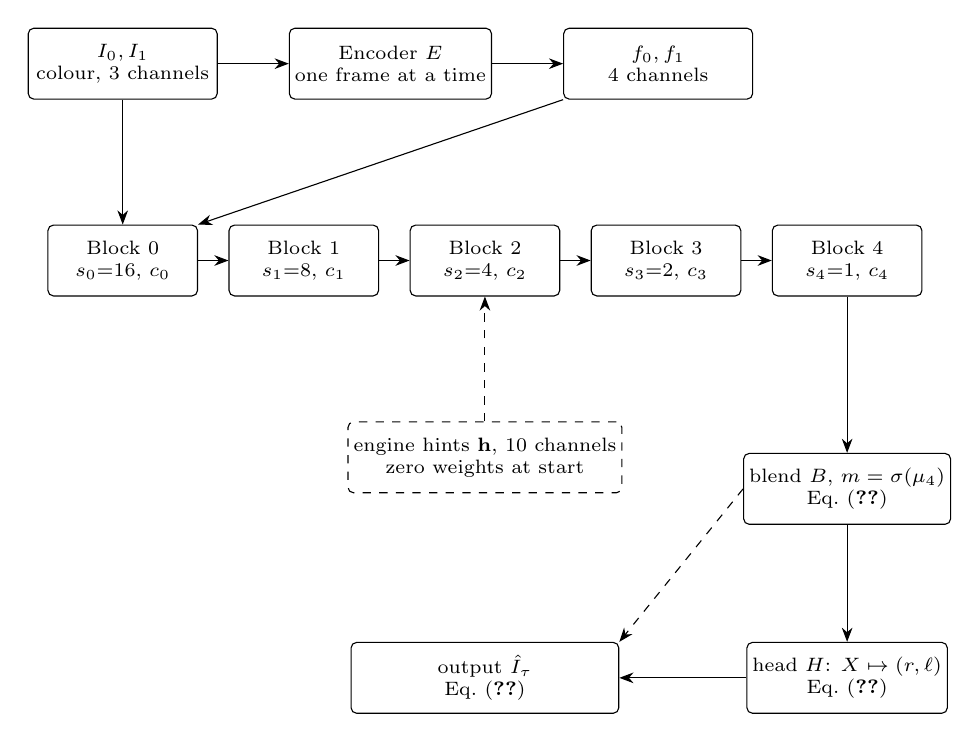
\begin{tikzpicture}[font=\scriptsize, box/.style={draw, rounded corners=2pt, align=center, minimum height=9mm, minimum width=19mm, inner sep=2pt},
  dashbox/.style={box, dashed}, arr/.style={-{Stealth[length=1.8mm]}}]
\node[box, minimum width=24mm] (in) at (0,0) {$I_0,I_1$\\colour, 3 channels};
\node[box, minimum width=24mm] (enc) at (3.4,0) {Encoder $E$\\one frame at a time};
\node[box, minimum width=24mm] (feat) at (6.8,0) {$f_0,f_1$\\4 channels};
\node[box] (b0) at (0,-2.5) {Block 0\\$s_0{=}16$, $c_0$};
\node[box] (b1) at (2.3,-2.5) {Block 1\\$s_1{=}8$, $c_1$};
\node[box] (b2) at (4.6,-2.5) {Block 2\\$s_2{=}4$, $c_2$};
\node[box] (b3) at (6.9,-2.5) {Block 3\\$s_3{=}2$, $c_3$};
\node[box] (b4) at (9.2,-2.5) {Block 4\\$s_4{=}1$, $c_4$};
\node[dashbox, minimum width=24mm] (hint) at (4.6,-5.0) {engine hints $\mathbf h$, 10 channels\\zero weights at start};
\node[box, minimum width=24mm] (blend) at (9.2,-5.4) {blend $B$, $m=\sigma(\mu_4)$\\Eq.~\eqref{eq:fgm-blend}};
\node[box, minimum width=24mm] (head) at (9.2,-7.8) {head $H$: $X\mapsto(r,\ell)$\\Eq.~\eqref{eq:fgm-head-in}};
\node[box, minimum width=34mm] (out) at (4.6,-7.8) {output $\hat I_\tau$\\Eq.~\eqref{eq:fgm-out}};
\draw[arr] (in.east) -- (enc.west);
\draw[arr] (enc.east) -- (feat.west);
\draw[arr] (in.south) -- (b0.north);
\draw[arr] (feat.south west) -- (b0.north east);
\draw[arr] (b0.east) -- (b1.west);
\draw[arr] (b1.east) -- (b2.west);
\draw[arr] (b2.east) -- (b3.west);
\draw[arr] (b3.east) -- (b4.west);
\draw[arr, dashed] (hint.north) -- (b2.south);
\draw[arr] (b4.south) -- (blend.north);
\draw[arr] (blend.south) -- (head.north);
\draw[arr] (head.west) -- (out.east);
\draw[arr, dashed] (blend.west) -- (out.north east);
\end{tikzpicture}
\caption{IFNet with the head. The encoder runs once per frame. Block $k$ takes the warped frames and features under the current flow, the previous mask and features, and $\tau$ (Eqs.~\eqref{eq:fgm-block0} and \eqref{eq:fgm-blockk}), and it outputs $\Delta_k$, $\mu_k$ and $\varphi_k$ (Eq.~\eqref{eq:fgm-blockout}). Engine hints enter every block through zero-initialised weights (\cref{sec:fgm-hints}). Block 4 gives the blend $B$, and the half-resolution head gives the residual $r$ and the UI logit, which form the output (Eqs.~\eqref{eq:fgm-head-in} and \eqref{eq:fgm-out}). The block scales and widths shown are those of the \tier{high} tier}\label{fig:fgm-ifnet}
\end{figure}

\subsection{RIFE 4.26 weights and the reproduction check}\label{sec:fgm-weights}

The weights are RIFE 4.26's archive, published in the author's Hugging Face repository. The downloader checks the SHA-256 hash of the archive and then of the \texttt{flownet.pkl} file inside it, and it loads the state dictionary with \texttt{weights\_only=True}, so the file cannot run code. The parameter names and shapes of the \tier{high} tier equal RIFE's, so every tensor is loaded by name. Where a tensor of a tier is smaller than its RIFE counterpart, the loader copies the leading slice along every dimension, the minimum of the two sizes. Where RIFE has more residual blocks than the tier, the first $n$ blocks are copied and the rest are ignored. Tensors that have no RIFE counterpart keep their initialisation, and the hint input columns keep their zero weights (\cref{sec:fgm-hints}). For the \tier{high} tier the loader reports 153 tensors copied exactly and 5 copied with a slice. The five sliced tensors are the first convolutions of the blocks, which are widened by the 10 hint channels, and no tensor is missing.

\emph{Reproduction check.} The check compares the \tier{high} tier with RIFE 4.26's own network code, the \texttt{IFNet\_HDv3} module of the archive, on the same inputs and with no engine data. RIFE's warp function is not in the archive, so the check recreates it with the grid convention of \cref{eq:fgm-warp}. The inputs are a random $8\times12$ image upsampled bicubically to $128\times192$ as $I_0$, and $I_0$ rolled by $(2,5)$ pixels as $I_1$, at $\tau=1/2$. The repository's check accepts a difference below $10^{-4}$ between the blend $B$ and RIFE's merged output in float32 on the CPU, and the agreement it measures is below $10^{-5}$. It also checks that the residual head and the hints add nothing at initialisation (\cref{sec:fgm-hints,sec:fgm-output}). The check tests the network code against RIFE's network code. It does not test the warp against RIFE's own kernel, and it does not test the delivered output of the generator, which differs from the blend (\cref{sec:fgm-output}).

\subsection{Tiers and channel-slice inheritance}\label{sec:fgm-tiers}

\Cref{tab:fgm-tiers} lists the four tiers. The \tier{high} tier has RIFE's widths, residual depth and block layout, and it is the one that starts from RIFE 4.26's network. The smaller tiers are narrower, with fewer residual blocks per block and a narrower head. Each tier is the generator of \cref{eq:fgm-task} with its own widths, residual depth, head width and flow line limit.

\begin{table}[!htbp]
\caption{Frame-generation tiers. Widths are the channel counts of blocks 0 to 4, $n$ the residual blocks per block, $c_h$ the head width, $L$ the flow line limit of \cref{eq:fgm-scale}, and GMAC the multiply-accumulates per 1080p output frame (every convolution, warps excluded), with flow at the scale the tier uses at 1080p}\label{tab:fgm-tiers}
\begin{tabular*}{\textwidth}{@{\extracolsep\fill}lllrrrr}
\toprule
Tier & Widths $c_0,\dots,c_4$ & $n$ & $c_h$ & $L$ & Params & GMAC \\
\midrule
\tier{igpu} & 64, 48, 32, 24, 16 & 3 & 12 & 576 & \Res{fg.model_tiers.igpu.params} & \Res{fg.model_tiers.igpu.gmac_per_1080p_frame} \\
\tier{low} & 96, 64, 48, 32, 16 & 4 & 16 & 576 & \Res{fg.model_tiers.low.params} & \Res{fg.model_tiers.low.gmac_per_1080p_frame} \\
\tier{mid} & 128, 96, 64, 48, 24 & 6 & 24 & 1152 & \Res{fg.model_tiers.mid.params} & \Res{fg.model_tiers.mid.gmac_per_1080p_frame} \\
\tier{high} & 192, 128, 96, 64, 32 & 8 & 32 & 1152 & \Res{fg.model_tiers.high.params} & \Res{fg.model_tiers.high.gmac_per_1080p_frame} \\
\bottomrule
\end{tabular*}
\end{table}

\emph{Channel-slice inheritance.} A smaller tier starts from RIFE's weights through the copy rule of \cref{sec:fgm-weights}. The narrower tensors take the leading channels of RIFE's tensor along each channel dimension, so the output channels of a block and the input channels of the next layer keep the same ordering. For the \tier{igpu} tier the loader reports 13 tensors with exact shapes and 70 sliced, for the \tier{low} tier 13 and 85, and for the \tier{mid} tier 13 and 115, with no missing tensor. The head has no RIFE counterpart, so it starts from its initialisation in every tier. The inheritance is a heuristic. Nothing forces RIFE's leading channels to be the best subset for a narrower network, and the ablation without inheritance (\cref{sec:fgm-ablate}) is the test of how much it matters.

\subsection{Flow-resolution caps and their cost}\label{sec:fgm-caps}

Estimating flow at full resolution is the most expensive part of the network, so every tier caps the number of image lines at which it estimates flow. A frame of height $H$ lines is halved until it fits under the tier's limit $L$, as RIFE's own scale argument allows:
\begin{equation}
s(H)=2^{-j^\ast},\qquad j^\ast=\min\big\{\,j\in\mathbb N_0:\,H\,2^{-j}\le L\,\big\},\label{eq:fgm-scale}
\end{equation}
with $L=576$ lines for the \tier{igpu} and \tier{low} tiers and $L=1152$ lines for the \tier{mid} and \tier{high} tiers. At 1080 lines the \tier{igpu} and \tier{low} tiers therefore estimate flow at $s=1/2$ (540 lines), and the \tier{mid} and \tier{high} tiers at $s=1$. The 256-pixel training crops and video up to 576 lines keep full-resolution flow in every tier. The frames are downsampled by $s$ before the encoder and the blocks, the flow hints are multiplied by $s$, and the flows that come out are upsampled and multiplied by $1/s$ to return to pixels. The head, the warps and the output stay at full resolution.

The convolution cost of the encoder and the blocks scales with the pixel count of the frames they see, so it scales with $s^2$. The head does not change. \Cref{tab:fgm-cap} gives the consequence at 1080p, counted with the same hooks as \cref{tab:fgm-tiers}. The cap removes more than half of the flow-path cost of the \tier{igpu} and \tier{low} tiers. For the \tier{low} tier the head is about a third of the capped cost, so the head matters most for the smallest tiers.

\begin{table}[!htbp]
\caption{Cost per 1080p generated frame of the tiers with the flow cap of \cref{eq:fgm-scale} and with full-resolution flow (GMAC, warps excluded). The encoder column counts both real frames, as the repository's tier table does, so one encoder pass is half of it. The head is the residual head of \cref{sec:fgm-output}}\label{tab:fgm-cap}
\begin{tabular*}{\textwidth}{@{\extracolsep\fill}lrrrrr}
\toprule
Tier & Flow scale & Capped total & Full-flow total & Encoder (two frames) & Head \\
\midrule
\tier{igpu} & \Res{fg.model_tiers.igpu.flow_scale_1080p} & \Res{fg.model_tiers.igpu.gmac_per_1080p_frame} & 20.4 & \Res{fg.model_tiers.igpu.gmac_per_frame_encoder} & 2.9 \\
\tier{low} & \Res{fg.model_tiers.low.flow_scale_1080p} & \Res{fg.model_tiers.low.gmac_per_1080p_frame} & 25.5 & \Res{fg.model_tiers.low.gmac_per_frame_encoder} & 4.5 \\
\tier{mid} & \Res{fg.model_tiers.mid.flow_scale_1080p} & \Res{fg.model_tiers.mid.gmac_per_1080p_frame} & 44.3 & \Res{fg.model_tiers.mid.gmac_per_frame_encoder} & 8.5 \\
\tier{high} & \Res{fg.model_tiers.high.flow_scale_1080p} & \Res{fg.model_tiers.high.gmac_per_1080p_frame} & 76.7 & \Res{fg.model_tiers.high.gmac_per_frame_encoder} & 13.8 \\
\bottomrule
\end{tabular*}
\end{table}

\subsection{Engine hints and their zero initialisation}\label{sec:fgm-hints}

When an engine provides data, the generator receives them as extra input channels of every IFNet block. \Cref{tab:fgm-hints} lists the ten channels in the order of the code. The signal channels are multiplied by their availability, so an absent signal contributes zero, and the flags tell the network which case it is in.

\emph{Motion priors.} If a point moves with constant velocity between $I_0$ and $I_1$, its displacement from $I_1$ to $I_0$ is $M_1$, and at time $\tau$ its displacement to $I_0$ is $\tau M_1$ and to $I_1$ is $(\tau-1)M_1$. The priors are exact only for linear motion, so the network has to learn when to trust them. The zero initialisation below lets it start from a working point.

\emph{Camera-only flow and late latching.} The camera flow $C$ is the displacement that the camera motion alone induces on the static background, from the target pixel to $I_1$. Let $A_t$ be the background affine map from screen to texture at time $t$ (\cref{sec:data-synth}), with normalised coordinates $x\in[-1,1]^2$. Then
\begin{equation}
C(x)=\tfrac{P}{2}\big(A_1^{-1}(A_\tau(x))-x\big),
\end{equation}
where $P$ is the frame size in pixels, so that $P/2$ converts normalised displacements to pixels for a $P\times P$ frame. Object motion is absent from $C$. At display time an engine knows the camera pose of the frame it is about to show, so the pose can be latched just before generation and supplied as this prior. In the synthetic training the prior uses the exact background trajectory at $\tau$. For real video the camera availability is zero, so the prior is never present.

\emph{Depth.} The depth channel is the inverse depth of $I_1$ normalised by its median, $d_1=1/(1+d/\operatorname{median}(d))$, so that a pixel at the median depth has the value one half. It is defined only for the synthetic renderer, where the depth is exact.

\emph{Availability.} Each availability flag is set per sample, and the signal channels are multiplied by the flags. Withholding a signal in training is therefore the same as an engine that does not provide it. The withholding rates are in \cref{tab:fgm-probs}.

\begin{table}[!htbp]
\caption{Sampling probabilities of the frame-generation training data, with the configuration names used in the saved files, or the constant in the code where no configuration name exists}\label{tab:fgm-probs}
{\footnotesize\begin{tabular*}{\textwidth}{@{\extracolsep\fill}lrl}
\toprule
Quantity & Value & Configuration or constant \\
\midrule
Real share of each GPU batch & \Res{fg.config.cfg.p_real} (19 of 48) & \texttt{p\_real} \\
Extrapolation, both sample kinds & \Res{fg.config.cfg.p_extrap} & \texttt{p\_extrap} \\
Random $\tau$ for synthetic interpolation & \Res{fg.config.cfg.p_tau} & \texttt{p\_tau}, $\tau\sim U[0.15,0.85]$ \\
Multi-frame share of real interpolation & \Res{fg.config.cfg.p_mfg} & \texttt{p\_mfg} \\
Camera reversal & \Res{fg.config.cfg.p_flip} & \texttt{p\_flip} \\
Scene cut & \Res{fg.config.cfg.p_cut} & \texttt{p\_cut} \\
UI overlay & \Res{fg.config.cfg.p_ui} & \texttt{p\_ui} \\
Menu, given a UI overlay & \Res{fg.config.cfg.p_menu} & \texttt{p\_menu} \\
Withhold motion vector (synthetic) & \Res{fg.config.cfg.p_drop_mv} & \texttt{p\_drop\_mv} \\
Withhold motion vector (real) & \Res{fg.config.cfg.p_drop_mv_real} & \texttt{p\_drop\_mv\_real} \\
Withhold depth (synthetic) & 0.30 & default argument in \texttt{set\_availability} \\
Withhold camera prior (extrapolation) & 0.20 & constant in \texttt{set\_availability} \\
UI slot filled / tile changed at $t=1$ & 0.70 / 0.30 & \texttt{ui\_layer} \\
\bottomrule
\end{tabular*}}
\end{table}

\paragraph{Zero-initialisation argument.} Let $W^{\mathbf h}_k$ be the weights of the first convolution of block $k$ that multiply the hint channels, and let every other weight of the \tier{high} tier equal RIFE's. The claim is that with $W^{\mathbf h}_k=0$ for every $k$, the blend $B$ does not depend on $\mathbf h$ and equals RIFE 4.26's blend. The argument is by induction over the blocks. Block 0 receives the same input as in RIFE, so its first convolution computes $z=W_x*x+W^{\mathbf h}_0*\mathbf h+b$ with $W^{\mathbf h}_0=0$, which equals RIFE's pre-activation $W_x*x+b$. The later layers of the block see only $z$, so the block outputs $(\Delta_0,\mu_0,\varphi_0)$ equal RIFE's. The induction step is the same for block $k$, because the warps and features that enter block $k$ are functions of the earlier outputs only. The blend of \cref{eq:fgm-blend} is then RIFE's blend. The head adds nothing at initialisation, because its last layer has zero weights and bias $(0,0,0,-4)$ (\cref{sec:fgm-output}). The gradient with respect to the hint columns is $\partial L/\partial W^{\mathbf h}_k=\sum_p \delta_k(p)\,\mathbf h(p)^{\top}$, summed over the sampled positions $p$, where $\delta_k$ is the gradient at the first-layer output. This is not zero when the hints are non-zero and the loss is sensitive to block $k$, so the hint columns leave zero at the first update. The fresh model therefore reproduces RIFE's blend, and then learns from the engine data.

\subsection{Head, UI weight and output}\label{sec:fgm-output}

The head turns the warped frames into a residual colour and a UI logit. Its input is the full-resolution stack of the two real frames, the two warps under the final flow, the blend weight and the last features:
\begin{equation}
X=\big[I_0,\,I_1,\,\mathcal W(I_0,F_4^0),\,\mathcal W(I_1,F_4^1),\,m,\,\varphi_4\big]\qquad(21\text{ channels}).\label{eq:fgm-head-in}
\end{equation}
A stride-2 $3\times3$ convolution with $c_h$ channels and LeakyReLU, two residual blocks at half resolution with the design of \cref{sec:fgm-ifnet}, and a $4\times4$ transposed convolution with stride 2 give four output channels, $(r,\ell)=H(X)$. Here $r$ is the residual colour and $\ell$ the UI logit. The head starts with a zero transposed-convolution weight and bias $(0,0,0,-4)$, so $r=0$ and $\ell=-4$ at initialisation, and the UI weight $u=\sigma(\ell)$ is about $0.018$. The output is
\begin{equation}
\hat I_\tau=u\odot I_1+(1-u)\odot\big(B+r\big),\qquad u=\sigma(\ell),\label{eq:fgm-out}
\end{equation}
with the blend $B$ of \cref{eq:fgm-blend}. This is \cref{M-eq:fg} of the article.

The UI weight is a soft mask in $[0,1]$, not a hard classification. Training pushes $u$ towards one on HUD, subtitle and menu pixels, where the UI mask of \cref{eq:fgm-ui-bce} is one, and towards zero elsewhere, so that those pixels come from the newest real frame $I_1$. The starting value means that a fresh model already mixes a small fraction of $I_1$ into every pixel. The delivered output of a fresh model therefore differs from the blend by $u\odot(I_1-B)$, which is small but not zero. This is why the reproduction check of \cref{sec:fgm-weights} compares the blend and not the output.

Evaluation clamps the output to $[0,1]$ before computing metrics. Training does not clamp, so the loss sees the unclamped output.

\emph{UI layer compositing.} When an engine renders the HUD separately from the scene, it can supply HUD-less real frames and the UI layer for the newest state, as premultiplied colour $c$ and alpha $\alpha$. The generator then runs on the HUD-less frames, and the displayed frame is $\hat I_\tau(1-\alpha)+c$. In the design this is applied to every displayed frame of the layer's sequence. The evaluation applies it to the generated frame only (\cref{sec:fgm-test}).

\subsection{Per-frame encoder reuse}\label{sec:fgm-encoder}

The encoder of \cref{eq:fgm-enc} depends on one frame, so a running sequence can encode each real frame once and reuse its features. The IFNet forward pass takes optional precomputed features for this, but no caller in the repository passes them. Training, evaluation and the exported graph all encode both frames (\cref{sec:fgm-export}).

The cost accounting follows from this. The encoder column of \cref{tab:fgm-cap} counts two frames, so one pass per real frame is half the column. With one generated frame per real frame, reuse replaces two encoder passes per generated frame by one.

\subsection{Scene-cut gate}\label{sec:fgm-cut}

\UnderRevision{} The gate decides when the generator should not generate. When two real frames look as if a scene cut lies between them, it outputs the newest real frame $I_1$ instead of $\hat I_\tau$. The repository marks this stage as a known weakness. Its thresholds are calibrated on synthetic adjacent pairs only, so the calibration does not cover real content or wider frame gaps.

The score combines a colour-distribution distance, which needs no motion, with a motion-compensated difference, which is used when $M_1$ is available. Let $Y(x)=(16+65.481R(x)+128.553G(x)+24.966B(x))/255$ be the limited-range luma of an RGB pixel with values in $[0,1]$, and let $h(I)\in\mathbb R^{32}$ be the fraction of pixels whose luma falls in each of 32 equal bins of $[0,1]$. The histogram distance and the motion-compensated difference are
\begin{align}
d_{\rm h}(I_0,I_1)&=\tfrac12\big\|h(I_0)-h(I_1)\big\|_1\in[0,1],\label{eq:fgm-hist}\\
d_{\rm m}(I_0,I_1,M_1)&=\frac{1}{3HW}\sum_{x,c}\big|I_1(x,c)-\mathcal W(I_0,M_1)(x,c)\big|.\label{eq:fgm-hist-m}
\end{align}
The two scores are
\begin{equation}
S_{\rm mv}=d_{\rm h}+2\,d_{\rm m},\qquad S_0=d_{\rm h},\label{eq:fgm-score}
\end{equation}
and the gate is
\begin{equation}
g=\begin{cases}\mathbf 1[S_{\rm mv}>\theta_{\rm mv}] & \text{if }a_{\rm mv}=1,\\ \mathbf 1[S_0>\theta_0] & \text{otherwise,}\end{cases}\label{eq:fgm-gate}
\end{equation}
where $\mathbf 1[\cdot]$ is one when its condition holds and zero otherwise. Without motion vectors the histogram distance alone is used, because a raw frame difference would read ordinary fast motion as a cut. The gate lives in the evaluation code, and it is not part of the exported graph.

\emph{Calibration.} Each threshold is set separately on synthetic pairs, so that continuous motion is a false alarm on about one pair in a hundred.
\begin{enumerate}
\item Draw four batches of up to 64 validation stills. For each batch, generate interpolation pairs at $\tau=1/2$ with motion from all four speed classes, no camera reversal and no UI, and with a cut probability of one half. Each pair is labelled cut or continuous. This gives 256 pairs, about half of them cuts.
\item Compute $S_{\rm mv}$ with the exact motion vector and $S_0$ for every pair.
\item For each score, sort the scores of the continuous pairs in ascending order and take the element at 0-based index $\lfloor0.99(n-1)\rfloor$, where $n$ is the number of continuous pairs. This element is the threshold $\theta$.
\item Report the detection rate, which is the share of cut pairs whose score exceeds $\theta$.
\end{enumerate}
The calibrated values are part of the results (\cref{sec:fgr}). When the gate fires, the output is the newest real frame,
\begin{equation}
\hat I_\tau\quad\leftarrow\quad I_1\qquad\text{if } g=1.\label{eq:fgm-gated}
\end{equation}

\subsection{Latency model and pacing}\label{sec:fgm-pacing}

\UnderRevision{} The latency numbers are timed on one data-centre GPU in eager PyTorch, and the pacing model is a simulation with assumed scheduling. The latency terms are those of \cref{sec:bg-latency}. The repository marks in-engine latency on target hardware as not measured. The model therefore answers what frame generation does to the displayed rate and to two latencies, under the stated assumptions.

The model is a discrete-event simulation of a GPU-bound loop with just-in-time CPU scheduling, in which the CPU starts each frame's work so that the GPU never queues frames, on a variable-refresh display. Its parameters are in \cref{tab:fgm-pacing}. The modes are \emph{native} (no generation), \emph{interpolation} (a generated frame between two real frames, with the newer real frame held), \emph{extrapolation} (a generated frame after the newest real frame, with nothing held) and \emph{extrapolation with late latching} (extrapolation whose camera is sampled just before generation).

\begin{table}[!htbp]
\caption{Parameters of the pacing model, as set in the simulation code and the notebook. The generation time $T_{\rm gen}$ is the measured one-generated-frame time of the \tier{low} tier at 1080p (\cref{sec:fgr}). The temporal super-resolution time $T_{\rm sr}$ is zero, because this pacing run has no such stage}\label{tab:fgm-pacing}
\begin{tabular*}{\textwidth}{@{\extracolsep\fill}lll}
\toprule
Symbol & Value & Meaning \\
\midrule
$R_0$ & 33.3, 25.0, 16.7\,ms & base render time per real frame (30, 40 and 60 fps renders) \\
$C_{\rm cpu}$ & 4.0\,ms & CPU time per frame before rendering starts \\
$c_v$ & 0.08 & log-normal spread of the render time \\
$T_{\rm pres}$ & 1.0\,ms & present time \\
$T_{\rm sr}$ & 0 & temporal super-resolution time \\
$T_{\rm gen}$ & measured & frame generation time per generated frame \\
$N$ & 2000 & simulated real frames per run \\
seed & 0 & random seed of the render times \\
\bottomrule
\end{tabular*}
\end{table}

The simulation runs as follows.
\begin{enumerate}
\item For each real frame $j=1,\dots,N$, draw the render time $R_j=R_0\exp(c_v z_j)$, where $z_j$ is standard normal.
\item Set the GPU time $g_j=R_j+T_{\rm sr}+T_{\rm gen}\,\mathbf 1[\text{mode}\neq\text{native}]$ and the frame period $\pi_j=\max(C_{\rm cpu},g_j)$.
\item Let $t_j$ be the time of the input sample, which is the current simulation time.
\item Set the time at which the rendered real frame is ready, $a_j=t_j+C_{\rm cpu}+R_j+T_{\rm sr}$.
\item In the \emph{native} mode, display the real frame at $p^{\rm r}_j=a_j+T_{\rm pres}$.
\item In the \emph{interpolation} mode, display the generated frame at $p^{\rm g}_j=a_j+T_{\rm gen}+T_{\rm pres}$, and hold the real frame until $p^{\rm r}_j=p^{\rm g}_j+\pi_j/2$.
\item In the \emph{extrapolation} mode, display the real frame at $p^{\rm r}_j=a_j+T_{\rm pres}$, and the generated frame at $p^{\rm g}_j=p^{\rm r}_j+\pi_j/2$.
\item In the \emph{extrapolation with late latching} mode, proceed as in step 7, and sample the camera of the generated frame at $t^{\rm cam}_j=p^{\rm g}_j-T_{\rm gen}-T_{\rm pres}$, the moment generation starts.
\item Record the displayed frames and the latency samples below, and advance the simulation time by $t\leftarrow t+\pi_j$.
\end{enumerate}
The rates are computed on the displayed times after the first tenth of the displayed sequence, so that start-up does not count. With $\Delta_i$ the gaps between consecutive displayed times, the displayed frame rate and the gap variation are $\mathrm{fps}=1000/\overline\Delta$ and $\mathrm{CV}=\operatorname{sd}(\Delta)/\overline\Delta$, in milliseconds for $\Delta$.

Three latencies are reported. The game input latency is the time from an input sample to the display of the real frame that reflects it, averaged over the real frames of the run,
\begin{equation}
L_{\rm game}=\operatorname{mean}_j\big(p^{\rm r}_j-t_j\big).\label{eq:fgm-lat-game}
\end{equation}
The camera latency is the same kind of time, measured to each displayed frame that counts as reflecting the camera. In the code a native frame counts with its real display. An interpolated frame counts with its generated display only, on the assumption that the generated frame already moves half way toward the camera of the newer frame. An extrapolated frame counts with both its real and its generated display, and with late latching the generated display is measured from $t^{\rm cam}_j$:
\begin{equation}
L_{\rm cam}=\begin{cases}\operatorname{mean}_j\big(p^{\rm r}_j-t_j\big) & \text{native},\\[2pt] \operatorname{mean}_j\big(p^{\rm g}_j-t_j\big) & \text{interpolation},\\[2pt] \tfrac12\Big(\operatorname{mean}_j\big(p^{\rm r}_j-t_j\big)+\operatorname{mean}_j\big(p^{\rm g}_j-t_j\big)\Big) & \text{extrapolation},\\[2pt] \tfrac12\Big(\operatorname{mean}_j\big(p^{\rm r}_j-t_j\big)+\operatorname{mean}_j\big(p^{\rm g}_j-t^{\rm cam}_j\big)\Big) & \text{late latching.}\end{cases}\label{eq:fgm-lat-cam}
\end{equation}
The content age averages the time from the input sample to every displayed frame, real or generated,
\begin{equation}
A=\operatorname{mean}_p\big(p-t\big)\quad\text{over all displayed frames }p.\label{eq:fgm-lat-age}
\end{equation}
Each latency is also reported at its 95th percentile over the samples.

The arithmetic estimate of a network's time at a sustained throughput $F$ in TFLOPS, is $T_{\rm est}=2G/F$ milliseconds, for a frame that costs $G$ GMAC, because one multiply-accumulate is two floating-point operations. The repository uses $F=4$ TFLOPS for an assumed integrated GPU. The estimate scales the GMAC with pixel count, so at 1440p it ignores the flow cap of \cref{eq:fgm-scale}.

\begin{figure}[!htbp]
\centering
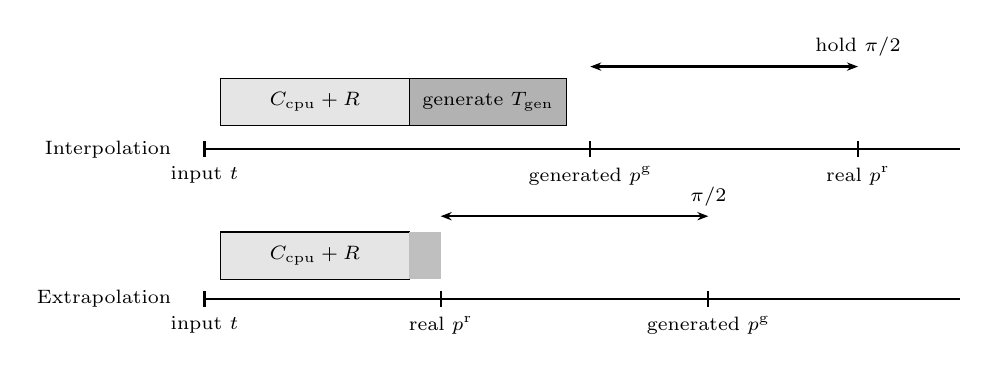
\begin{tikzpicture}[font=\scriptsize, x=1cm, y=1cm,
  tick/.style={thick},
  lab/.style={font=\scriptsize, align=center},
  bar/.style={draw, minimum height=6mm, inner sep=1pt}]
\node[anchor=east, lab] at (-0.3,1.9) {Interpolation};
\draw[thick] (0,1.9) -- (9.6,1.9);
\node[bar, fill=black!10, minimum width=2.4cm] at (1.4,2.5) {$C_{\rm cpu}+R$};
\node[bar, fill=black!30, minimum width=2.0cm] at (3.6,2.5) {generate $T_{\rm gen}$};
\draw[tick] (0,1.8) -- (0,2.0);
\node[lab, below] at (0,1.8) {input $t$};
\draw[tick] (4.9,1.8) -- (4.9,2.0);
\node[lab, below] at (4.9,1.8) {generated $p^{\rm g}$};
\draw[tick] (8.3,1.8) -- (8.3,2.0);
\node[lab, below] at (8.3,1.8) {real $p^{\rm r}$};
\draw[{Stealth[length=1.4mm]}-{Stealth[length=1.4mm]}, thick] (4.9,2.95) -- (8.3,2.95) node[above, lab] {hold $\pi/2$};
\node[anchor=east, lab] at (-0.3,0.0) {Extrapolation};
\draw[thick] (0,0.0) -- (9.6,0.0);
\node[bar, fill=black!10, minimum width=2.4cm] at (1.4,0.55) {$C_{\rm cpu}+R$};
\fill[black!25] (2.6,0.25) rectangle (3.0,0.85);
\draw[tick] (0,-0.1) -- (0,0.1);
\node[lab, below] at (0,-0.1) {input $t$};
\draw[tick] (3.0,-0.1) -- (3.0,0.1);
\node[lab, below] at (3.0,-0.1) {real $p^{\rm r}$};
\draw[tick] (6.4,-0.1) -- (6.4,0.1);
\node[lab, below] at (6.4,-0.1) {generated $p^{\rm g}$};
\draw[{Stealth[length=1.4mm]}-{Stealth[length=1.4mm]}, thick] (3.0,1.05) -- (6.4,1.05) node[above, lab] {$\pi/2$};
\end{tikzpicture}
\caption{Timeline of one input sample in the two generation modes, schematic and not to scale. In interpolation the generated frame needs the newest real frame, and the real frame is held for half a period, so it is shown after the generated frame. In extrapolation the real frame is shown as soon as it is rendered, and the generated frame follows half a period later, with the generation time $T_{\rm gen}$ inside that period. The grey bar at $T_{\rm pres}$ in the extrapolation row is the present time. The labels are the symbols of \cref{tab:fgm-pacing}}\label{fig:fgm-timeline}
\end{figure}

\cref{fig:fgm-timeline} shows the two modes. Interpolation adds $T_{\rm gen}$ to the time of the generated frame and delays the real frame by half a period. Extrapolation adds no delay to the real frame and adds half a period to the generated frame, which is shown after the real frame.

\subsection{Training samples}\label{sec:fgm-samples}

In the main stages each of the two GPUs takes its own batch of 48 samples per step, under distributed data parallel training. A batch holds 19 real quads and 29 synthetic samples, since the real share \Res{fg.config.cfg.p_real} of 48 rounds to 19, drawn at random without replacement from the caches. Still crops are $512\times512$ pixels cut from the textures of \cref{sec:data-synth}, and quads are four frames of $256\times256$ pixels from the sequence sources of \cref{sec:data}, both after the random downscale of \cref{sec:data}. The cache sizes are in \cref{sec:fgr}.

\paragraph{Synthetic samples.} Each synthetic sample is one scene of the renderer of \cref{sec:data-synth}, rendered at $256\times256$ pixels with four anti-aliasing samples per pixel for $I_0$, $I_1$ and the target. The background is one still. The foreground is the still of the neighbouring sample in the batch, visible through a procedural alpha mask in 85 percent of samples, and a flat colour in 25 percent of samples. The construction of one sample is as follows.
\begin{enumerate}
\item Draw the camera reversal with probability \Res{fg.config.cfg.p_flip}. A reversal reverses the camera velocity after $t=1$.
\item Draw extrapolation with probability \Res{fg.config.cfg.p_extrap}. If it is extrapolation, set $\tau=1.5$. Otherwise set $\tau=1/2$, or with probability \Res{fg.config.cfg.p_tau} draw $\tau$ uniformly from $[0.15,0.85]$.
\item Render $I_0$ at $t=0$, $I_1$ at $t=1$ and the target at $t=\tau$.
\item Compute the exact motion vector $M_1$, which is the flow from $I_1$ to $I_0$, the exact flows $F_{\tau\to0}$ and $F_{\tau\to1}$ with their validity masks (visible and inside the view), the camera flow $C$ and the inverse depth $d_1$.
\item Draw a scene cut with probability \Res{fg.config.cfg.p_cut}. A cut replaces $I_1$, $M_1$ and $d_1$ by those of the neighbouring sample, sets the target to the replaced $I_1$, and sets the validity masks to zero.
\item Draw UI overlays with probability \Res{fg.config.cfg.p_ui}. Four UI slots are each filled with probability 0.7 by a tile from a bank of 256 text, bar and crosshair tiles of $160\times28$ pixels, and 30 percent of the filled slots change their tile at $t=1$. A full-screen menu panel of alpha 0.6 and colour 0.05 is drawn with probability \Res{fg.config.cfg.p_menu} given a UI overlay, which is 1.5 percent of all samples. The tiles are alpha-composited into $I_0$ with the state at $t=0$, into $I_1$ with the state at $t=1$, and into the target with the state at $t=1$. The UI mask is the maximum of the two alphas.
\item Withhold the signals according to \cref{tab:fgm-probs}, and set the camera availability to zero for every interpolation sample.
\end{enumerate}

\paragraph{Real quads.} Each real sample is a window of four consecutive frames from one of the sequence sources of \cref{sec:data}, decoded and cut to $256\times256$ pixels. The window is flipped horizontally and vertically with probability one half each, and its flow fields are flipped with it, with the vector components negated along each flipped axis. The sample then takes one of three forms.
\begin{enumerate}
\item With probability \Res{fg.config.cfg.p_extrap}, extrapolation: $I_0=k$, $I_1=k+2$ and target $k+3$, at $\tau=1.5$.
\item Otherwise, with probability \Res{fg.config.cfg.p_mfg}, multi-frame generation: $I_0=k$, $I_1=k+3$, and the target is $k+1$ or $k+2$ with equal probability, at $\tau=1/3$ or $2/3$.
\item Otherwise interpolation: $I_0=k$, $I_1=k+2$ and target $k+1$, at $\tau=1/2$.
\end{enumerate}
The flows come from the RAFT optical-flow network \cite{teed2020raft}, in the small variant that torchvision ships with its weights. The cache computes four flows per quad, $k+2\to k$, $k+1\to k$, $k+1\to k+2$ and $k+3\to k+2$, at the $256\times256$ crop size, and stores them at half resolution, in pixels of the full grid, by two-by-two average pooling. Every quad carries these four flows, including the TartanAir and Sintel quads that have exact flows in the frame decoder, because the quad cache does not use those flows. The motion vector $M_1$ is the flow $k+2\to k$. The flows $F_{\tau\to0}$ and $F_{\tau\to1}$ are $k+1\to k$ and $k+1\to k+2$ for interpolation, and $k+3\to k+2$ for extrapolation. An extrapolated sample has no label from the target to $I_0$, so its $F_{\tau\to0}$ validity is zero. A multi-frame sample has no flow label, so its $M_1$ and both flow validities are zero. A real sample has no depth and no camera prior, so its depth and camera availabilities are zero. Every pixel of a real flow is valid, because the cache computes no validity mask.

\paragraph{Availability and the plain-video case.} \Cref{tab:fgm-probs} gives the withholding rates. Synthetic samples withhold the motion vector with probability \Res{fg.config.cfg.p_drop_mv} and the depth with probability 0.3, and they keep the camera prior with probability 0.8 on extrapolation samples only. Real samples withhold the motion vector with probability \Res{fg.config.cfg.p_drop_mv_real} when a flow label exists, and they never have depth or a camera prior. The validation batches are fixed, with \Res{fg.config.cfg.val_bs} stills and \Res{fg.config.cfg.val_bs} quads in each of \Res{fg.config.cfg.val_batches} batches, drawn with a seed of 54321. Each is evaluated twice, once with its availabilities and once with all of them set to zero, which is plain video.

\subsection{Training objective}\label{sec:fgm-loss}

The objective is a weighted sum of six terms, with a unit weight on the first,
\begin{equation}
\mathcal L=\mathcal L_{\rm pix}+0.5\,\mathcal L_{\rm cen}+0.1\,\mathcal L_{\rm lp}+0.01\,\mathcal L_{\rm flow}+0.2\,\mathcal L_{\rm ui}+0.5\,\mathcal L_{\rm kd},\label{eq:fgm-total}
\end{equation}
where each term is a mean over the batch. \Cref{tab:fgm-loss} gives the definitions, and the paragraphs below give the formulas.

\begin{table}[!htbp]
\caption{Training losses of the frame generator, with weights and the samples to which each term applies}\label{tab:fgm-loss}
\begin{tabular*}{\textwidth}{@{\extracolsep\fill}lp{0.42\textwidth}rp{0.30\textwidth}}
\toprule
Term & Quantity & Weight & Applies to \\
\midrule
$\mathcal L_{\rm pix}$ & Charbonnier penalty, $\varepsilon=10^{-3}$ & 1 & every sample \\
$\mathcal L_{\rm cen}$ & soft census distance, $7\times7$ window & \Res{fg.config.cfg.w_census} & every sample \\
$\mathcal L_{\rm lp}$ & LPIPS with AlexNet, on the clipped output & \Res{fg.config.cfg.w_lpips} & every sample, when the package loads \\
$\mathcal L_{\rm flow}$ & flow L1 on valid pixels, weight 1 (synthetic) or 1/4 (real) & \Res{fg.config.cfg.w_flow} & every sample with flow labels \\
$\mathcal L_{\rm ui}$ & binary cross-entropy on the UI mask, positive weight 4 & \Res{fg.config.cfg.w_ui} & every sample \\
$\mathcal L_{\rm kd}$ & distillation from the \tier{high} teacher & \Res{fg.config.cfg.w_distill} & students only \\
\bottomrule
\end{tabular*}
\end{table}

\emph{Charbonnier.} With the target $I_\tau$ and the output $\hat I_\tau$, $\mathcal L_{\rm pix}=\operatorname{mean}\sqrt{(\hat I_\tau-I_\tau)^2+\varepsilon^2}$, where the mean runs over every colour value. This is a smooth form of the L1 penalty. It is a smooth edge-preserving potential of the Charbonnier family \cite{charbonnier1997deterministic}.

\emph{Census.} For a grey image $g=0.299R+0.587G+0.114B$, the census vector at pixel $x$ has one soft-ternary entry per offset $\delta$ in the $7\times7$ window $D$, which has 49 offsets including zero,
\begin{equation}
c(x,\delta)=\frac{g(x+\delta)-g(x)}{\sqrt{0.81+\big(g(x+\delta)-g(x)\big)^2}}.\label{eq:fgm-census}
\end{equation}
The census distance at a pixel is $\rho(x)=\operatorname{mean}_{\delta\in D}\,d/(0.1+d)$, with $d=\big(c_{\hat I}(x,\delta)-c_{I}(x,\delta)\big)^2$. The loss $\mathcal L_{\rm cen}$ is the mean of $\rho$ over the image with a border of three pixels removed on each side. Census distances are insensitive to brightness offsets, the property for which the census loss was introduced for unsupervised flow \cite{meister2018unflow}. The soft-ternary normalisation and the robust distance are the repository's own choices.

\emph{LPIPS.} $\mathcal L_{\rm lp}$ is the LPIPS distance with the AlexNet network and version 0.1 of its calibration weights \cite{zhang2018lpips}, applied to the output clipped to $[0,1]$ and to the target, and averaged over the batch. The weight is zero when the package does not load, and the saved configuration records that.

\emph{Flow.} The flow term is the weighted L1 error of both flows over the valid pixels,
\begin{align}
\mathcal L_{\rm flow}&=\frac{\sum_x\sum_{c}\big|\hat F_{0,c}(x)-F_{0,c}(x)\big|\,v_0(x)}{2\sum_x v_0(x)+1}\nonumber\\
&\quad+\frac{\sum_x\sum_{c}\big|\hat F_{1,c}(x)-F_{1,c}(x)\big|\,v_1(x)}{2\sum_x v_1(x)+1},\label{eq:fgm-flow}
\end{align}
where $c\in\{x,y\}$ runs over the two flow components.
where $v_i=w\,\mathrm{valid}_i$ with $w=1$ for synthetic samples and $w=1/4$ for real samples. The denominator counts the valid pixels and not their weights, so a real sample contributes a quarter of the error of a synthetic one at the same pixel error.

\emph{UI.} With $y(x)=\mathbf 1[\mathrm{ui}(x)>0.5]$ for the UI mask $\mathrm{ui}=\max(\alpha_0,\alpha_1)$ of \cref{sec:fgm-samples},
\begin{equation}
\mathcal L_{\rm ui}=-\operatorname{mean}\Big[4\,y\log\sigma(\ell)+(1-y)\log\big(1-\sigma(\ell)\big)\Big],\label{eq:fgm-ui-bce}
\end{equation}
which is the binary cross-entropy on the UI logit $\ell$, with the positive term weighted by four to up-weight the rarer UI pixels.

\emph{Distillation.} When a teacher checkpoint is given, the teacher is the \tier{high} tier with the same inputs and availabilities, run without gradients. With $\hat I^{\rm T}$ and $\hat F^{\rm T}_i$ the teacher output and flows,
\begin{equation}
\mathcal L_{\rm kd}=\operatorname{mean}\big|\hat I_\tau-\hat I^{\rm T}\big|+0.01\Big(\operatorname{mean}\big|\hat F_0-\hat F^{\rm T}_0\big|+\operatorname{mean}\big|\hat F_1-\hat F^{\rm T}_1\big|\Big).\label{eq:fgm-kd}
\end{equation}
Training a student to match a teacher's outputs in this way is distillation \cite{gou2021knowledge}. The 0.01 weight on the flows is a constant of the code, not a configuration value.

\subsection{Optimisation and schedule}\label{sec:fgm-schedule}

The optimiser is AdamW \cite{loshchilov2019adamw} with betas $(0.9,0.99)$ and weight decay \Res{fg.config.cfg.weight_decay} on all parameters. The gradient norm is clipped to \Res{fg.config.cfg.grad_clip} after unscaling. The forward pass runs under fp16 autocast with dynamic loss scaling, and the losses are computed in float32 \cite{micikevicius2018mixed}. The learning rate follows the fraction $p=t/T$ of the wall-clock budget $T$ already used. It rises linearly over the first \Res{fg.config.cfg.warmup_frac} of the budget and then decays with a cosine to a floor of $\mathrm{lr}_{\min}=10^{-6}$:
\begin{equation}
\mathrm{lr}(p)=\begin{cases}\mathrm{lr}_0\,\max(p/0.03,\,0.01) & p<0.03,\\ \mathrm{lr}_{\min}+\tfrac12(\mathrm{lr}_0-\mathrm{lr}_{\min})\big(1+\cos\pi q\big) & p\geq0.03,\end{cases}\qquad q=\frac{p-0.03}{0.97}.\label{eq:fgm-lr}
\end{equation}
A moving average of the weights, the exponential moving average (EMA), is updated after every step on the rank-0 model with decay $d_s=\min(0.999,(1+s)/(10+s))$ at step $s$, so the decay starts near zero and reaches \Res{fg.config.cfg.ema_decay}. Validation runs every $\min(8\,\mathrm{min},\max(T/6,60\,\mathrm{s}))$ and at the end of the budget. Each validation saves the latest weights, and the best weights by the selection metric, which is the mean of the PSNR with and without engine data (\cref{sec:fgm-test}). The run stops with an error after 200 consecutive steps with a non-finite loss. If a run exhausts GPU memory, it is retried once with half the batch for the rest of its budget.

Training follows two stages, listed in \cref{tab:fgm-runs}. First the \tier{high} tier is fine-tuned from RIFE 4.26 on both GPUs at a learning rate of \Res{fg.config.cfg.lr_teacher} and with no teacher, since it is the tier that starts from RIFE's network. Then the smaller tiers start from RIFE's leading slices and are trained with the full objective, including distillation from the EMA weights of the fine-tuned \tier{high} run, at a learning rate of \Res{fg.config.cfg.lr}. The \tier{low} tier, the main student, uses both GPUs. The \tier{igpu} and \tier{mid} tiers train side by side, one GPU each. The nominal budgets are those of the table, and the run scales them by one common factor below one, so that the whole pipeline fits the session. The saved configurations show the scaled budgets.

\begin{table}[!htbp]
\caption{Training runs of the frame generator, in stage order. Budgets are the nominal wall-clock times, and batches are per GPU}\label{tab:fgm-runs}
\begin{tabular*}{\textwidth}{@{\extracolsep\fill}llllrrr}
\toprule
Run & Tier & Initialisation & Distillation & Learning rate & Budget (min) & Batch \\
\midrule
\texttt{fg\_teacher} & \tier{high} & RIFE 4.26 & none & \Res{fg.config.cfg.lr_teacher} & \Res{fg.config.cfg.minutes.teacher} & 48 \\
\texttt{fg\_low} & \tier{low} & RIFE slices & \tier{high} & \Res{fg.config.cfg.lr} & \Res{fg.config.cfg.minutes.student} & 48 \\
\texttt{fg\_igpu} & \tier{igpu} & RIFE slices & \tier{high} & \Res{fg.config.cfg.lr} & \Res{fg.config.cfg.minutes.pair} & 48 \\
\texttt{fg\_mid} & \tier{mid} & RIFE slices & \tier{high} & \Res{fg.config.cfg.lr} & \Res{fg.config.cfg.minutes.pair} & 24 \\
six ablations & \tier{low} & see \cref{tab:fgm-abl} & see \cref{tab:fgm-abl} & \Res{fg.config.cfg.lr} & \Res{fg.config.cfg.minutes.ablation} & 48 \\
\bottomrule
\end{tabular*}
\end{table}

\subsection{Ablations}\label{sec:fgm-ablate}

Each ablation is a \tier{low} run with the same \Res{fg.config.cfg.minutes.ablation}-minute budget as the reference. Each changes one setting of the configuration (\cref{tab:fgm-abl}), and the ablation runs go in pairs, one run per GPU. All of them use the same wall-clock budget, so the run without distillation takes more steps, because it skips the teacher's forward pass.

\begin{table}[!htbp]
\caption{Ablations of the \tier{low} tier, with the configuration change of each relative to the reference (the saved \texttt{cfg\_abl\_*.json} files)}\label{tab:fgm-abl}
\begin{tabular*}{\textwidth}{@{\extracolsep\fill}lp{0.70\textwidth}}
\toprule
Run & Change from the reference \\
\midrule
\texttt{abl\_reference} & none, so distillation from the \tier{high} run and UI training are on \\
\texttt{abl\_no\_ui\_training} & no HUD, subtitle or menu overlays in training, and UI loss weight zero \\
\texttt{abl\_no\_motion\_prior} & motion vector and camera availability forced to zero in training (depth kept) \\
\texttt{abl\_extrap\_only} & every training sample is an extrapolation ($p_{\rm extrap}=1$) \\
\texttt{abl\_no\_distillation} & no teacher, so $\mathcal L_{\rm kd}$ is absent \\
\texttt{abl\_no\_inheritance} & no RIFE weights, so the IFNet starts from the default initialisation \\
\bottomrule
\end{tabular*}
\end{table}

The \texttt{abl\_no\_motion\_prior} model is evaluated without any engine data in both modes, because its training never supplied the motion vector or the camera prior. Validation scores are not compared across ablations, which share only the test suites (\cref{sec:fgm-test}).

\subsection{Fusion and ONNX export}\label{sec:fgm-export}

The re-parameterisation fusion of the temporal super-resolution network does not apply to the generator, since it has no such blocks. Fusion here is a copy in evaluation mode, and the check that fused and unfused outputs agree holds by construction. The fused weights are stored, and their fp16 copies are used for timing.

The export wrapper takes the two real frames, the motion vector, the depth, the camera prior, the time and the three availability flags, and returns the output frame,
\begin{equation}
\hat I_\tau=\mathrm{FG}\big(I_0,I_1,M_1,d_1,C,\tau,a_{\rm mv},a_{\rm cam},a_{\rm dep}\big).\label{eq:fgm-export}
\end{equation}
The exporter is TorchScript based, with opset 17, and the graph is static. The example input is $128\times128$ pixels for both exported models, the \tier{low} and \tier{igpu} tiers. The check runs ONNX Runtime on the CPU and compares it with PyTorch in float32 on the same example, and the difference is below $10^{-5}$ for both models. Two limits follow from the export. First, the flow scale of \cref{eq:fgm-scale} is decided from the frame height when the graph is traced, and a $128$-line example has $s=1$ for every tier. The exported graph therefore computes full-resolution flow, and a graph for a $1080$-line output must be exported at that size. Second, the exported graph encodes both real frames, so the reuse of \cref{sec:fgm-encoder} is not in it.

\subsection{Test protocol}\label{sec:fgm-test}

All evaluation uses the test split only. Every suite is evaluated in an \emph{engine} mode, where the batch carries the engine data that the suite has, and in a \emph{plain} mode, where the batch carries none, so that the generator sees ordinary video. The 3x multi-frame suites are plain only. \Cref{tab:fgm-suites} lists the suites. The synthetic suites use \Res{fg.config.cfg.eval.synthetic_per_suite} textures of $512\times512$ pixels from held-out game frames and DIV2K validation images, each rendered at $256\times256$ pixels. The real suites take up to \Res{fg.config.cfg.eval.real_clips} clips each, four times that for the Vimeo-90K triplets, and \Res{fg.config.cfg.eval.native_clips} at native resolution.

\begin{table}[!htbp]
\caption{Test suites of the frame generator. Modes are interpolation at $\tau=1/2$ (interp), extrapolation at $\tau=1.5$ (extrap) and 3x multi-frame generation (mfg3x, plain input only). The engine motion vector of real suites is exact for TartanAir and Sintel and estimated by RAFT otherwise}\label{tab:fgm-suites}
{\footnotesize\setlength{\tabcolsep}{3pt}\raggedright\begin{tabular*}{\textwidth}{@{\extracolsep\fill}p{0.23\textwidth}p{0.14\textwidth}p{0.14\textwidth}p{0.18\textwidth}p{0.22\textwidth}}
\toprule
Suite & Source & Crop (lines $\times$ width) & Modes & Notes \\
\midrule
\texttt{synthetic} & held-out textures & $256\times256$ & interp, extrap & the four speed classes, separately \\
\texttt{synthetic-ui} & held-out textures & $256\times256$ & interp, extrap & HUD and subtitle changes on every sample \\
\texttt{synthetic-menu} & held-out textures & $256\times256$ & interp, extrap & menu on every sample \\
\texttt{synthetic-cut} & held-out textures & $256\times256$ & interp, extrap & every sample is a cut \\
\texttt{synthetic-reversal} & held-out textures & $256\times256$ & extrap & every camera reverses, in engine mode with and without the camera prior \\
\texttt{vimeo\_triplet} & Vimeo-90K & $256\times448$ & interp & three frames per clip \\
\texttt{tartanair} & TartanAir & $480\times640$ & interp, extrap, mfg3x & exact motion vectors \\
\texttt{sintel} & MPI Sintel & $432\times1024$ & interp, extrap, mfg3x & exact motion vectors \\
\texttt{vid4} & Vid4 & $480\times704$ & interp, extrap, mfg3x & RAFT motion \\
\texttt{vimeo1080p} & Vimeo 1080p & $544\times960$ & interp, extrap, mfg3x & frames scaled to 544 lines \\
\texttt{vimeo1080p\_native} & Vimeo 1080p & $1072\times1904$ & interp, extrap, mfg3x & native resolution \\
\bottomrule
\end{tabular*}}
\end{table}

\emph{Clip selection.} A real clip is the first four frames of a candidate item (three for triplets), centre-cropped to the size of \cref{tab:fgm-suites}, after the downscale of the 544-line suite. Candidates are read in order, and a candidate is skipped when it cannot be decoded or when it has a defect. The defects are a blank frame, with a luma standard deviation below 2 on the 0 to 255 scale, a frozen pair, with a mean absolute luma difference below 0.1 on the same scale, and a cut, with half the L1 distance between the normalised 32-bin luma histograms of consecutive frames above 0.5. By this rule the test clips contain no cuts, which makes the gated share of \cref{sec:fgm-cut} a false-alarm rate. The sequences of TartanAir and Sintel are played backwards, so that their exact forward flow becomes the motion from the newest frame to the older one. The engine motion vector of $I_1$ is composed from two consecutive exact motion vectors, $M_1=m_{21}+\mathcal W(m_{10},m_{21})$, where $m_{ij}$ is the exact motion from frame $i$ to frame $j$.

On the other real suites the motion is RAFT-small from $I_1$ to $I_0$, estimated at full resolution up to a longer side of 1024 pixels. Beyond that the RAFT input is resized to a longer side of 1024 pixels, and its flow is scaled back, so the native suite's motion is estimated at reduced size. For real suites the occlusion mask of the target is estimated by RAFT with a forward-backward consistency test \cite{meister2018unflow}, and it is used by the metrics only. For synthetic suites the mask is exact.

\emph{Methods.} \Cref{tab:fgm-methods} lists the methods, how each is gated and what inputs each receives.

\begin{table}[!htbp]
\caption{Methods of the frame-generation test protocol and their inputs. The gate of \cref{eq:fgm-gate} replaces the output of a gated method by $I_1$. Baselines are never gated, and the frame repeat is $I_1$ itself, so gating it changes nothing}\label{tab:fgm-methods}
{\footnotesize\setlength{\tabcolsep}{3pt}\raggedright\begin{tabular*}{\textwidth}{@{\extracolsep\fill}p{0.22\textwidth}p{0.38\textwidth}p{0.14\textwidth}p{0.20\textwidth}}
\toprule
Method & Definition & Gated & Inputs \\
\midrule
frame repeat & $I_1$ & not applicable & both \\
frame average & $\tfrac12(I_0+I_1)$ & no & both \\
motion-vector reprojection & Eq.~\eqref{eq:fgm-analytic} with $\tau M_1$ and $(\tau-1)M_1$ & no & engine only \\
RIFE 4.26 unchanged & blend $B$ of \cref{eq:fgm-blend} & yes & colour only in both modes \\
\tier{high}, \tier{low}, \tier{igpu}, \tier{mid} & output $\hat I_\tau$ & yes & both \\
ablations & output $\hat I_\tau$ of each run & yes & both \\
UI layer (UI suites only) & $\hat I_\tau(1-\alpha)+c$ on HUD-less frames & yes & engine only \\
\bottomrule
\end{tabular*}}
\end{table}

The reprojection baseline is an analytic warp-and-blend that uses linear motion. The two frames are warped by the two priors, $W_0=\mathcal W(I_0,\tau M_1)$ and $W_1=\mathcal W(I_1,(\tau-1)M_1)$, and they are blended per pixel with a weight that prefers the warp agreeing with the other,
\begin{align}
\mathrm{Rep}(I_0,I_1,M_1)&=\mu\,\tfrac12(W_0+W_1)+(1-\mu)\,W_1,\label{eq:fgm-analytic}\\
\mu&=\sigma\big(40\,(0.1-\bar\epsilon)\big),\qquad \bar\epsilon=\operatorname{mean}_c\big|W_0-W_1\big|.\nonumber
\end{align}
Where the two warps disagree by more than about 0.1, the weight $\mu$ falls to zero and the result is $W_1$. This treats disagreeing pixels as occluded and gives them the newer frame, which is a heuristic. The baseline needs motion vectors, so it is absent in the plain mode. The networks use no engine data in the plain mode, and the RIFE reference is colour only in both modes, as its design requires.

\emph{Metrics.} Each sample gives the following values, which follow \cref{sec:bg-metrics}, with the generated frame clipped to $[0,1]$ before each metric.
\begin{itemize}
\item PSNR on RGB, $10\log_{10}(1/\mathrm{MSE})$, with the mean squared error over all colour values, and also over the UI pixels or over the occluded pixels when those exist. The occluded pixels are those not visible in $I_1$ by the target's occlusion mask, and a sample counts only if it has more than 50 of them.
\item SSIM with an $11\times11$ Gaussian window of standard deviation 1.5, computed per colour channel with $C_1=0.01^2$ and $C_2=0.03^2$, and averaged \cite{wang2004ssim}.
\item LPIPS with AlexNet \cite{zhang2018lpips}.
\item Interpolation error, the root-mean-square difference on the 0 to 255 scale \cite{baker2011middlebury}.
\item UI ghosting rate, the share of UI pixels whose largest colour error exceeds 0.1.
\item Motion magnitude, the mean length of $M_1$ in pixels, recorded for each sample.
\end{itemize}
The temporal consistency of the displayed sequence is measured on the interpolation suites in the plain mode, with RAFT-small flows \cite{teed2020raft}. For each clip, the flow from $I_0$ to the output and the flow from the output to $I_1$ are compared with the flow from $I_0$ to the true target and from the target to $I_1$. The per-clip value is the mean of the two mean norms of the flow differences, in pixels. It is a sequence version of the tOF measure of TecoGAN \cite{chu2020tecogan}, not the function in the library, and it is reported per clip, because a few large-motion clips can dominate a suite mean.

The Middlebury comparison uses the 12 sequences of the Middlebury ``other'' interpolation set \cite{baker2011middlebury}. It takes frames 10 and 11 as inputs and the middle frame 10i11 as the ground truth. It runs on the CPU with colour input only, after training, with the saved checkpoints. Frames of 380 to 480 lines are below the flow line limit of every tier, so this comparison estimates flow at full resolution for every tier.

\emph{Gated samples and the reporting rule.} A gated output equals $I_1$ exactly, so a sample is gated when the gate of \cref{eq:fgm-gate} fires and the PSNR of the RIFE output equals that of the frame repeat. The notebook does not build these tables. They are made after the run from the per-sample file. The gate is shared by every method on the same batch. The as-saved table includes gated samples, and the not-gated table excludes them. The test clips contain no cuts by construction, so every gated real sample is a false alarm. Including those samples would measure the gate's false-alarm rate, not how well each generator interpolates, so the not-gated table is the one that compares generators. The gated share is reported for each suite, mode and input mode.

\emph{Latency protocol.} The per-frame latency of each fused fp16 generator is the mean of 100 timed forward passes at batch size 1, after 10 warm-up passes, with CUDA events and the cuDNN autotuner on. The inputs contain every engine signal. The timing runs at $1920\times1080$ and at $2560\times1440$, and the $1920\times1080$ time of the \tier{low} tier feeds the pacing model of \cref{sec:fgm-pacing}.

\section{Frame generation and real-time cost: results}\label{sec:fgr}

This section reports every saved output of the frame-generation notebook and of the Middlebury comparison that was run after it. The notebook trains the frame generator, calibrates its scene-cut detector, evaluates every network on the test split and writes the metric files, the plots and the predictions that the tables and figures below show. The method is described in \cref{sec:fgm}, the metrics in \cref{sec:bg-metrics} and the latency concepts in \cref{sec:bg-latency}. For each result we state what is measured, what the table or figure shows, the mechanism where the design explains it, what the result does not show and the number of samples when that number is small.

Two conventions apply throughout. The \tier{high} tier is the notebook's teacher, a network with RIFE 4.26's widths that starts from the pre-trained RIFE weights. The notebook calls the \tier{low} tier the student, and the tables use the article's tier names. Each test result also has two views. The all-sample view averages every sample, including those where the cut gate replaced the network output with the newest real frame. The not-gated view averages only the samples the gate left alone, and it is the view the article uses for plain video. \Cref{sec:fgr-gate} explains why.

\Preliminary{} All frame-generation results come from one run. It started on \Res{run.neural-frame-generation.start} on two Tesla T4 GPUs with \Res{fg.hardware.cpu_count} CPU cores and PyTorch \Res{fg.hardware.torch}. It took \Res{run.neural-frame-generation.hours} hours to the end of the evaluation, and the summary cell recorded \Res{fg.summary.run_hours} hours. The Middlebury comparison in \cref{sec:fgr-mb} was run afterwards on a CPU with the same checkpoints. Because there is one run, no finding below has a repeat that would show its run-to-run variation.

\subsection{Training runs}\label{sec:fgr-train}

The notebook trained the \tier{high} tier for \Res{fg.config.cfg.minutes.teacher} minutes, the \tier{low} tier for \Res{fg.config.cfg.minutes.student} minutes, and the \tier{igpu} and \tier{mid} tiers in parallel for \Res{fg.config.cfg.minutes.pair} minutes each. Before training it built the caches and probed the batch size. After the \tier{low} tier it ran six ablations of \Res{fg.config.cfg.minutes.ablation} minutes each, in three parallel pairs. \Cref{fig:fgr-stages} gives the stage times. The caches took \Res{fg.stage_times.caches.minutes} minutes against a build budget of \Res{fg.config.cfg.cache.build_min} minutes, and the test suites and the evaluation took \Res{fg.stage_times.test_suites.minutes} and \Res{fg.stage_times.evaluation.minutes} minutes.

\begin{figure}[!htbp]
\centering
\includegraphics[width=0.7\textwidth]{\FgOut/plots/stage_times.png}
\caption{Wall-clock minutes per stage of the frame-generation run, from the notebook's stage timer}\label{fig:fgr-stages}
\end{figure}

Every validation round scored the checkpoint on held-out batches with engine data, without it, and on the interpolation, extrapolation and UI regions. The checkpoint metric is the mean of the engine and plain scores, so each best value is an average over the two input modes. \Cref{tab:fgr-runs} lists the best round of every run. \Preliminary{} The \tier{high} tier reached \Res{fg.best_validation.fg_teacher.val_psnr} dB, the \tier{mid} tier \Res{fg.best_validation.fg_mid.val_psnr} dB, the \tier{low} tier \Res{fg.best_validation.fg_low.val_psnr} dB and the \tier{igpu} tier \Res{fg.best_validation.fg_igpu.val_psnr} dB. For the \tier{high} tier the engine and plain scores differ by \ResAbsDiff{fg.best_validation.fg_teacher.val_psnr_engine}{fg.best_validation.fg_teacher.val_psnr_plain} dB, so the engine dropout during training leaves the two input modes close on the validation batches.

\begin{table}[!htbp]
\caption{Training runs (the \tier{high} row is the notebook's teacher): validation PSNR (dB) of the best checkpoint by the checkpoint metric (mean of the engine and plain validation PSNR), with the round and the minutes of its run. The rounds and minutes columns give the validation rounds and the elapsed training time}\label{tab:fgr-runs}
\scriptsize\setlength{\tabcolsep}{2pt}
\begin{tabular*}{\textwidth}{@{\extracolsep\fill}lrrrrrrrrr}
\toprule
Run & Rounds & Min. & Best round & Val. PSNR & Engine & Plain & Interp. & Extrap. & UI \\
\midrule
\tier{high} & \Res{fg.history_fg_teacher.rounds} & \Res{fg.history_fg_teacher.elapsed_min.last} & \Res{fg.best_validation.fg_teacher.round} & \Res{fg.best_validation.fg_teacher.val_psnr} & \Res{fg.best_validation.fg_teacher.val_psnr_engine} & \Res{fg.best_validation.fg_teacher.val_psnr_plain} & \Res{fg.best_validation.fg_teacher.val_psnr_interp} & \Res{fg.best_validation.fg_teacher.val_psnr_extrap} & \Res{fg.best_validation.fg_teacher.val_psnr_ui} \\
\tier{low} & \Res{fg.history_fg_low.rounds} & \Res{fg.history_fg_low.elapsed_min.last} & \Res{fg.best_validation.fg_low.round} & \Res{fg.best_validation.fg_low.val_psnr} & \Res{fg.best_validation.fg_low.val_psnr_engine} & \Res{fg.best_validation.fg_low.val_psnr_plain} & \Res{fg.best_validation.fg_low.val_psnr_interp} & \Res{fg.best_validation.fg_low.val_psnr_extrap} & \Res{fg.best_validation.fg_low.val_psnr_ui} \\
\tier{mid} & \Res{fg.history_fg_mid.rounds} & \Res{fg.history_fg_mid.elapsed_min.last} & \Res{fg.best_validation.fg_mid.round} & \Res{fg.best_validation.fg_mid.val_psnr} & \Res{fg.best_validation.fg_mid.val_psnr_engine} & \Res{fg.best_validation.fg_mid.val_psnr_plain} & \Res{fg.best_validation.fg_mid.val_psnr_interp} & \Res{fg.best_validation.fg_mid.val_psnr_extrap} & \Res{fg.best_validation.fg_mid.val_psnr_ui} \\
\tier{igpu} & \Res{fg.history_fg_igpu.rounds} & \Res{fg.history_fg_igpu.elapsed_min.last} & \Res{fg.best_validation.fg_igpu.round} & \Res{fg.best_validation.fg_igpu.val_psnr} & \Res{fg.best_validation.fg_igpu.val_psnr_engine} & \Res{fg.best_validation.fg_igpu.val_psnr_plain} & \Res{fg.best_validation.fg_igpu.val_psnr_interp} & \Res{fg.best_validation.fg_igpu.val_psnr_extrap} & \Res{fg.best_validation.fg_igpu.val_psnr_ui} \\
\midrule
Reference & \Res{fg.history_abl_reference.rounds} & \Res{fg.history_abl_reference.elapsed_min.last} & \Res{fg.best_validation.abl_reference.round} & \Res{fg.best_validation.abl_reference.val_psnr} & \Res{fg.best_validation.abl_reference.val_psnr_engine} & \Res{fg.best_validation.abl_reference.val_psnr_plain} & \Res{fg.best_validation.abl_reference.val_psnr_interp} & \Res{fg.best_validation.abl_reference.val_psnr_extrap} & \Res{fg.best_validation.abl_reference.val_psnr_ui} \\
No UI & \Res{fg.history_abl_no_ui_training.rounds} & \Res{fg.history_abl_no_ui_training.elapsed_min.last} & \Res{fg.best_validation.abl_no_ui_training.round} & \Res{fg.best_validation.abl_no_ui_training.val_psnr} & \Res{fg.best_validation.abl_no_ui_training.val_psnr_engine} & \Res{fg.best_validation.abl_no_ui_training.val_psnr_plain} & \Res{fg.best_validation.abl_no_ui_training.val_psnr_interp} & \Res{fg.best_validation.abl_no_ui_training.val_psnr_extrap} & n/a \\
No prior & \Res{fg.history_abl_no_motion_prior.rounds} & \Res{fg.history_abl_no_motion_prior.elapsed_min.last} & \Res{fg.best_validation.abl_no_motion_prior.round} & \Res{fg.best_validation.abl_no_motion_prior.val_psnr} & \Res{fg.best_validation.abl_no_motion_prior.val_psnr_engine} & \Res{fg.best_validation.abl_no_motion_prior.val_psnr_plain} & \Res{fg.best_validation.abl_no_motion_prior.val_psnr_interp} & \Res{fg.best_validation.abl_no_motion_prior.val_psnr_extrap} & \Res{fg.best_validation.abl_no_motion_prior.val_psnr_ui} \\
Extrap. only & \Res{fg.history_abl_extrap_only.rounds} & \Res{fg.history_abl_extrap_only.elapsed_min.last} & \Res{fg.best_validation.abl_extrap_only.round} & \Res{fg.best_validation.abl_extrap_only.val_psnr} & \Res{fg.best_validation.abl_extrap_only.val_psnr_engine} & \Res{fg.best_validation.abl_extrap_only.val_psnr_plain} & n/a & \Res{fg.best_validation.abl_extrap_only.val_psnr_extrap} & \Res{fg.best_validation.abl_extrap_only.val_psnr_ui} \\
No distill. & \Res{fg.history_abl_no_distillation.rounds} & \Res{fg.history_abl_no_distillation.elapsed_min.last} & \Res{fg.best_validation.abl_no_distillation.round} & \Res{fg.best_validation.abl_no_distillation.val_psnr} & \Res{fg.best_validation.abl_no_distillation.val_psnr_engine} & \Res{fg.best_validation.abl_no_distillation.val_psnr_plain} & \Res{fg.best_validation.abl_no_distillation.val_psnr_interp} & \Res{fg.best_validation.abl_no_distillation.val_psnr_extrap} & \Res{fg.best_validation.abl_no_distillation.val_psnr_ui} \\
No inherit. & \Res{fg.history_abl_no_inheritance.rounds} & \Res{fg.history_abl_no_inheritance.elapsed_min.last} & \Res{fg.best_validation.abl_no_inheritance.round} & \Res{fg.best_validation.abl_no_inheritance.val_psnr} & \Res{fg.best_validation.abl_no_inheritance.val_psnr_engine} & \Res{fg.best_validation.abl_no_inheritance.val_psnr_plain} & \Res{fg.best_validation.abl_no_inheritance.val_psnr_interp} & \Res{fg.best_validation.abl_no_inheritance.val_psnr_extrap} & \Res{fg.best_validation.abl_no_inheritance.val_psnr_ui} \\
\botrule
\end{tabular*}
\end{table}


\Preliminary{} Every run's best round was its last validation round, so no run had converged when its budget ended. The \tier{low} tier had \Res{fg.history_fg_low.rounds} validation rounds and was still improving at the last one, after \Res{fg.history_fg_low.elapsed_min.last} minutes. The tier ranking therefore partly reflects the budgets, and a longer run would change the gaps between the tiers by an amount this run cannot measure.

\begin{figure*}[!htbp]
\centering
\includegraphics[width=\textwidth]{\FgOut/plots/training_curves.png}
\caption{Validation PSNR (dB, left) against elapsed minutes for every run, with the ablations dashed, and the training loss of the four main runs (right). Training losses of the students include the distillation term and are not comparable with the teacher's loss}\label{fig:fgr-training}
\end{figure*}

\Observation{} \Cref{fig:fgr-training} shows the same picture as the table. The \tier{high} tier rises quickly and flattens late in its budget, the \tier{mid} tier follows, and the \tier{igpu} tier stays lowest. The ablations run for 30 minutes and their curves stop there, with the reference reaching \Res{fg.history_abl_reference.val_psnr.max} dB. The training losses fall in every run. They are plotted for the shape of each curve, and their levels do not compare the tiers, because the students add a distillation term that the teacher does not have.

The batch probe (\cref{tab:fgr-batch}) chose the largest batch whose peak memory stayed below 75 percent of the GPU memory, a margin the notebook keeps for the losses and data that the probe leaves out. For the \tier{high} tier alone the largest such batch was 48 per GPU, at \Res{fg.batch_probe.teacher.48.peak_vram_pct} percent peak memory, and a batch of 64 reached \Res{fg.batch_probe.teacher.64.peak_vram_pct} percent and was rejected. With the teacher alongside, the \tier{low} student also used 48, at \Res{fg.batch_probe.student.48.peak_vram_pct} percent. The \tier{mid} tier used half the student's batch, with a minimum of 8, by the notebook's rule. \Observation{} Throughput levelled off once the batch reached 16 samples, so the larger batches bought little speed.

\begin{table}[!htbp]
\caption{Batch-size probe on GPU 0: peak allocated memory as a share of the GPU memory and training samples per second for the \tier{high} teacher and for the \tier{low} student with the teacher alongside. The probe picks the largest batch with at most 75 percent peak memory}\label{tab:fgr-batch}
\footnotesize\setlength{\tabcolsep}{3pt}
\begin{tabular*}{\textwidth}{@{\extracolsep\fill}lrrrr}
\toprule
Batch per GPU & \tier{high} peak memory (\%) & \tier{high} samples/s & \tier{low} peak memory (\%) & \tier{low} samples/s \\
\midrule
4 & \Res{fg.batch_probe.teacher.4.peak_vram_pct} & \Res{fg.batch_probe.teacher.4.samples_per_s} & \Res{fg.batch_probe.student.4.peak_vram_pct} & \Res{fg.batch_probe.student.4.samples_per_s} \\
8 & \Res{fg.batch_probe.teacher.8.peak_vram_pct} & \Res{fg.batch_probe.teacher.8.samples_per_s} & \Res{fg.batch_probe.student.8.peak_vram_pct} & \Res{fg.batch_probe.student.8.samples_per_s} \\
12 & \Res{fg.batch_probe.teacher.12.peak_vram_pct} & \Res{fg.batch_probe.teacher.12.samples_per_s} & \Res{fg.batch_probe.student.12.peak_vram_pct} & \Res{fg.batch_probe.student.12.samples_per_s} \\
16 & \Res{fg.batch_probe.teacher.16.peak_vram_pct} & \Res{fg.batch_probe.teacher.16.samples_per_s} & \Res{fg.batch_probe.student.16.peak_vram_pct} & \Res{fg.batch_probe.student.16.samples_per_s} \\
24 & \Res{fg.batch_probe.teacher.24.peak_vram_pct} & \Res{fg.batch_probe.teacher.24.samples_per_s} & \Res{fg.batch_probe.student.24.peak_vram_pct} & \Res{fg.batch_probe.student.24.samples_per_s} \\
32 & \Res{fg.batch_probe.teacher.32.peak_vram_pct} & \Res{fg.batch_probe.teacher.32.samples_per_s} & \Res{fg.batch_probe.student.32.peak_vram_pct} & \Res{fg.batch_probe.student.32.samples_per_s} \\
48 & \Res{fg.batch_probe.teacher.48.peak_vram_pct} & \Res{fg.batch_probe.teacher.48.samples_per_s} & \Res{fg.batch_probe.student.48.peak_vram_pct} & \Res{fg.batch_probe.student.48.samples_per_s} \\
64 & \Res{fg.batch_probe.teacher.64.peak_vram_pct} & \Res{fg.batch_probe.teacher.64.samples_per_s} & \Res{fg.batch_probe.student.64.peak_vram_pct} & \Res{fg.batch_probe.student.64.samples_per_s} \\
\botrule
\end{tabular*}
\end{table}


No run failed and no run wrote an out-of-memory log, so every run trained at the batch the probe chose.

\subsection{Interpolation}\label{sec:fgr-interp}

Interpolation generates the frame at $\tau=0.5$ between two real frames. The test suites are the Vimeo-90K triplets, the Vimeo-1080p clips at 544 lines and at their native 1072 lines, Vid4, TartanAir, Sintel, the synthetic suite of game-like scenes and, after the run, the twelve Middlebury sequences. Each suite is run on plain input, with engine data where the suite has it, and the baselines are frame repetition, frame averaging and, with engine data, motion-vector reprojection.

\subsubsection{Why the not-gated view is reported}\label{sec:fgr-gate}

\Preliminary{} The test clips contain no scene cuts, so every real sample that the cut gate replaced is a false alarm, and the replaced output is the newest real frame rather than an interpolation. Including those outputs measures the gate and not the generator. \Cref{tab:fgr-gate-effect} shows the effect. On TartanAir one gated sample out of ten lowers the all-sample mean of RIFE 4.26 by \ResAbsDiff{fg.test_results.tartanair.interp.plain.rife_4_26.psnr}{fg.test_per_sample.tartanair.interp.plain.rife_4_26.psnr} dB. The not-gated view therefore reports the generators on the samples where generation actually runs. The gate is evaluated separately in \cref{sec:fgr-cut}.

\begin{table}[!htbp]
\caption{Effect of the cut gate on plain interpolation (PSNR, dB): all samples against the samples the gate left alone. Gated samples carry the newest real frame, so they lower the all-sample mean of every method that the gate covers}\label{tab:fgr-gate-effect}
\footnotesize\setlength{\tabcolsep}{3pt}
\begin{tabular*}{\textwidth}{@{\extracolsep\fill}lrrrrr}
\toprule
Suite & Gated / samples & RIFE, all & RIFE, kept & \tier{high}, all & \tier{high}, kept \\
\midrule
Synthetic & \Res{fg.cut_gate_rates.synthetic.interp.plain.gated} of \Res{fg.cut_gate_rates.synthetic.interp.plain.samples} & \Res{fg.test_results.synthetic.interp.plain.rife_4_26.psnr} & \Res{fg.test_per_sample.synthetic.interp.plain.rife_4_26.psnr} & \Res{fg.test_results.synthetic.interp.plain.high.psnr} & \Res{fg.test_per_sample.synthetic.interp.plain.high.psnr} \\
Vimeo-90K triplet & \Res{fg.cut_gate_rates.vimeo_triplet.interp.plain.gated} of \Res{fg.cut_gate_rates.vimeo_triplet.interp.plain.samples} & \Res{fg.test_results.vimeo_triplet.interp.plain.rife_4_26.psnr} & \Res{fg.test_per_sample.vimeo_triplet.interp.plain.rife_4_26.psnr} & \Res{fg.test_results.vimeo_triplet.interp.plain.high.psnr} & \Res{fg.test_per_sample.vimeo_triplet.interp.plain.high.psnr} \\
Vimeo-1080p, 544 lines & \Res{fg.cut_gate_rates.vimeo1080p.interp.plain.gated} of \Res{fg.cut_gate_rates.vimeo1080p.interp.plain.samples} & \Res{fg.test_results.vimeo1080p.interp.plain.rife_4_26.psnr} & \Res{fg.test_per_sample.vimeo1080p.interp.plain.rife_4_26.psnr} & \Res{fg.test_results.vimeo1080p.interp.plain.high.psnr} & \Res{fg.test_per_sample.vimeo1080p.interp.plain.high.psnr} \\
Vimeo-1080p, native & \Res{fg.cut_gate_rates.vimeo1080p_native.interp.plain.gated} of \Res{fg.cut_gate_rates.vimeo1080p_native.interp.plain.samples} & \Res{fg.test_results.vimeo1080p_native.interp.plain.rife_4_26.psnr} & \Res{fg.test_per_sample.vimeo1080p_native.interp.plain.rife_4_26.psnr} & \Res{fg.test_results.vimeo1080p_native.interp.plain.high.psnr} & \Res{fg.test_per_sample.vimeo1080p_native.interp.plain.high.psnr} \\
Vid4 & \Res{fg.cut_gate_rates.vid4.interp.plain.gated} of \Res{fg.cut_gate_rates.vid4.interp.plain.samples} & \Res{fg.test_results.vid4.interp.plain.rife_4_26.psnr} & \Res{fg.test_per_sample.vid4.interp.plain.rife_4_26.psnr} & \Res{fg.test_results.vid4.interp.plain.high.psnr} & \Res{fg.test_per_sample.vid4.interp.plain.high.psnr} \\
TartanAir & \Res{fg.cut_gate_rates.tartanair.interp.plain.gated} of \Res{fg.cut_gate_rates.tartanair.interp.plain.samples} & \Res{fg.test_results.tartanair.interp.plain.rife_4_26.psnr} & \Res{fg.test_per_sample.tartanair.interp.plain.rife_4_26.psnr} & \Res{fg.test_results.tartanair.interp.plain.high.psnr} & \Res{fg.test_per_sample.tartanair.interp.plain.high.psnr} \\
Sintel & \Res{fg.cut_gate_rates.sintel.interp.plain.gated} of \Res{fg.cut_gate_rates.sintel.interp.plain.samples} & \Res{fg.test_results.sintel.interp.plain.rife_4_26.psnr} & \Res{fg.test_per_sample.sintel.interp.plain.rife_4_26.psnr} & \Res{fg.test_results.sintel.interp.plain.high.psnr} & \Res{fg.test_per_sample.sintel.interp.plain.high.psnr} \\
\botrule
\end{tabular*}
\end{table}


\UnderRevision{} The gate also fires on samples without a cut. It replaced \Res{fg.cut_gate_rates.synthetic.interp.plain.gated} of \Res{fg.cut_gate_rates.synthetic.interp.plain.samples} plain synthetic samples, a share of \Res{fg.cut_gate_rates.synthetic.interp.plain.gated_share}, while its threshold was calibrated for one percent false alarms on continuous pairs. The gap between calibration and test is the reason the not-gated view is needed, and a gate that false-alarms at this rate is not deployable in its present form.

\subsubsection{Plain video}\label{sec:fgr-interp-plain}

\Cref{tab:fgr-interp-plain} gives the not-gated PSNR of every tier and baseline.

\begin{table}[!htbp]
\caption{Frame interpolation on plain video (no engine data), PSNR (dB), not-gated samples (kept of all samples in brackets). Bold marks the best deployable tier per row. Repeat is the newest real frame, average is the mean of the two real frames and RIFE 4.26 is the pre-trained network unchanged}\label{tab:fgr-interp-plain}
\footnotesize\setlength{\tabcolsep}{3pt}
\begin{tabular*}{\textwidth}{@{\extracolsep\fill}lrrrrrrr}
\toprule
Suite (kept of samples) & Repeat & Average & RIFE 4.26 & \tier{igpu} & \tier{low} & \tier{mid} & \tier{high} \\
\midrule
Synthetic (\Res{fg.test_per_sample.synthetic.interp.plain.kept} of \Res{fg.test_per_sample.synthetic.interp.plain.n}) & \Res{fg.test_per_sample.synthetic.interp.plain.repeat.psnr} & \Res{fg.test_per_sample.synthetic.interp.plain.average.psnr} & \Res{fg.test_per_sample.synthetic.interp.plain.rife_4_26.psnr} & \Res{fg.test_per_sample.synthetic.interp.plain.igpu.psnr} & \Res{fg.test_per_sample.synthetic.interp.plain.student.psnr} & \Res{fg.test_per_sample.synthetic.interp.plain.mid.psnr} & \textbf{\Res{fg.test_per_sample.synthetic.interp.plain.high.psnr}} \\
Vimeo-90K triplet (\Res{fg.test_per_sample.vimeo_triplet.interp.plain.kept} of \Res{fg.test_per_sample.vimeo_triplet.interp.plain.n}) & \Res{fg.test_per_sample.vimeo_triplet.interp.plain.repeat.psnr} & \Res{fg.test_per_sample.vimeo_triplet.interp.plain.average.psnr} & \Res{fg.test_per_sample.vimeo_triplet.interp.plain.rife_4_26.psnr} & \Res{fg.test_per_sample.vimeo_triplet.interp.plain.igpu.psnr} & \Res{fg.test_per_sample.vimeo_triplet.interp.plain.student.psnr} & \Res{fg.test_per_sample.vimeo_triplet.interp.plain.mid.psnr} & \textbf{\Res{fg.test_per_sample.vimeo_triplet.interp.plain.high.psnr}} \\
Vimeo-1080p, 544 lines (\Res{fg.test_per_sample.vimeo1080p.interp.plain.kept} of \Res{fg.test_per_sample.vimeo1080p.interp.plain.n}) & \Res{fg.test_per_sample.vimeo1080p.interp.plain.repeat.psnr} & \Res{fg.test_per_sample.vimeo1080p.interp.plain.average.psnr} & \Res{fg.test_per_sample.vimeo1080p.interp.plain.rife_4_26.psnr} & \Res{fg.test_per_sample.vimeo1080p.interp.plain.igpu.psnr} & \Res{fg.test_per_sample.vimeo1080p.interp.plain.student.psnr} & \Res{fg.test_per_sample.vimeo1080p.interp.plain.mid.psnr} & \textbf{\Res{fg.test_per_sample.vimeo1080p.interp.plain.high.psnr}} \\
Vimeo-1080p, native (\Res{fg.test_per_sample.vimeo1080p_native.interp.plain.kept} of \Res{fg.test_per_sample.vimeo1080p_native.interp.plain.n}) & \Res{fg.test_per_sample.vimeo1080p_native.interp.plain.repeat.psnr} & \Res{fg.test_per_sample.vimeo1080p_native.interp.plain.average.psnr} & \Res{fg.test_per_sample.vimeo1080p_native.interp.plain.rife_4_26.psnr} & \Res{fg.test_per_sample.vimeo1080p_native.interp.plain.igpu.psnr} & \Res{fg.test_per_sample.vimeo1080p_native.interp.plain.student.psnr} & \Res{fg.test_per_sample.vimeo1080p_native.interp.plain.mid.psnr} & \textbf{\Res{fg.test_per_sample.vimeo1080p_native.interp.plain.high.psnr}} \\
Vid4 (\Res{fg.test_per_sample.vid4.interp.plain.kept} of \Res{fg.test_per_sample.vid4.interp.plain.n}) & \Res{fg.test_per_sample.vid4.interp.plain.repeat.psnr} & \Res{fg.test_per_sample.vid4.interp.plain.average.psnr} & \Res{fg.test_per_sample.vid4.interp.plain.rife_4_26.psnr} & \Res{fg.test_per_sample.vid4.interp.plain.igpu.psnr} & \Res{fg.test_per_sample.vid4.interp.plain.student.psnr} & \Res{fg.test_per_sample.vid4.interp.plain.mid.psnr} & \textbf{\Res{fg.test_per_sample.vid4.interp.plain.high.psnr}} \\
TartanAir (\Res{fg.test_per_sample.tartanair.interp.plain.kept} of \Res{fg.test_per_sample.tartanair.interp.plain.n}) & \Res{fg.test_per_sample.tartanair.interp.plain.repeat.psnr} & \Res{fg.test_per_sample.tartanair.interp.plain.average.psnr} & \Res{fg.test_per_sample.tartanair.interp.plain.rife_4_26.psnr} & \Res{fg.test_per_sample.tartanair.interp.plain.igpu.psnr} & \Res{fg.test_per_sample.tartanair.interp.plain.student.psnr} & \Res{fg.test_per_sample.tartanair.interp.plain.mid.psnr} & \textbf{\Res{fg.test_per_sample.tartanair.interp.plain.high.psnr}} \\
Sintel (\Res{fg.test_per_sample.sintel.interp.plain.kept} of \Res{fg.test_per_sample.sintel.interp.plain.n}) & \Res{fg.test_per_sample.sintel.interp.plain.repeat.psnr} & \Res{fg.test_per_sample.sintel.interp.plain.average.psnr} & \Res{fg.test_per_sample.sintel.interp.plain.rife_4_26.psnr} & \Res{fg.test_per_sample.sintel.interp.plain.igpu.psnr} & \Res{fg.test_per_sample.sintel.interp.plain.student.psnr} & \Res{fg.test_per_sample.sintel.interp.plain.mid.psnr} & \textbf{\Res{fg.test_per_sample.sintel.interp.plain.high.psnr}} \\
\midrule
\botrule
\end{tabular*}
\end{table}


\Preliminary{} The \tier{high} tier is the best tier on every suite. It beats RIFE 4.26 by \ResAbsDiff{fg.test_per_sample.vimeo_triplet.interp.plain.high.psnr}{fg.test_per_sample.vimeo_triplet.interp.plain.rife_4_26.psnr} dB on the Vimeo-90K triplets, by \ResAbsDiff{fg.test_per_sample.vimeo1080p.interp.plain.high.psnr}{fg.test_per_sample.vimeo1080p.interp.plain.rife_4_26.psnr} dB on Vimeo-1080p at 544 lines, by \ResAbsDiff{fg.test_per_sample.vimeo1080p_native.interp.plain.high.psnr}{fg.test_per_sample.vimeo1080p_native.interp.plain.rife_4_26.psnr} dB at native resolution and by \ResAbsDiff{fg.test_per_sample.vid4.interp.plain.high.psnr}{fg.test_per_sample.vid4.interp.plain.rife_4_26.psnr} dB on Vid4. RIFE 4.26 stays ahead on TartanAir, by \ResAbsDiff{fg.test_per_sample.tartanair.interp.plain.high.psnr}{fg.test_per_sample.tartanair.interp.plain.rife_4_26.psnr} dB, and on Sintel, by \ResAbsDiff{fg.test_per_sample.sintel.interp.plain.high.psnr}{fg.test_per_sample.sintel.interp.plain.rife_4_26.psnr} dB. The Sintel gap rests on \Res{fg.test_per_sample.sintel.interp.plain.kept} kept samples, and the Vid4 margin rests on \Res{fg.test_per_sample.vid4.interp.plain.kept} samples, which makes it the least certain of the positive margins. On the synthetic suite RIFE 4.26 is also ahead, by \ResAbsDiff{fg.test_per_sample.synthetic.interp.plain.high.psnr}{fg.test_per_sample.synthetic.interp.plain.rife_4_26.psnr} dB, although the \tier{high} tier has the lower interpolation error there.

\Observation{} The two suites where RIFE 4.26 leads are the two with the fewest real training quads, which are Sintel with \Res{fg.caches.quad_sources.train.sintel} and TartanAir with \Res{fg.caches.quad_sources.train.tartanair} quads, against \Res{fg.caches.quad_sources.train.vimeo_septuplet} Vimeo-90K quads in the cache. This is a hypothesis about the training data mix. The run did not test it, and a run with those suites up-weighted would be needed to confirm it.

\Preliminary{} The \tier{mid} tier, at \Res{fg.model_tiers.mid.gmac_per_1080p_frame} GMAC per 1080p frame, is within 0.5 dB of RIFE 4.26 on five of the seven suites, counting Middlebury. The \tier{low} tier, at \Res{fg.model_tiers.low.gmac_per_1080p_frame} GMAC and with half of RIFE's channel widths, beats frame averaging on every suite and trails RIFE 4.26 by between \ResAbsDiff{fg.test_per_sample.vid4.interp.plain.student.psnr}{fg.test_per_sample.vid4.interp.plain.rife_4_26.psnr} dB on Vid4 and \ResAbsDiff{fg.test_per_sample.tartanair.interp.plain.student.psnr}{fg.test_per_sample.tartanair.interp.plain.rife_4_26.psnr} dB on TartanAir. The \tier{igpu} tier is barely above averaging on the two 1080p suites, by \ResAbsDiff{fg.test_per_sample.vimeo1080p.interp.plain.igpu.psnr}{fg.test_per_sample.vimeo1080p.interp.plain.average.psnr} dB at 544 lines and by \ResAbsDiff{fg.test_per_sample.vimeo1080p_native.interp.plain.igpu.psnr}{fg.test_per_sample.vimeo1080p_native.interp.plain.average.psnr} dB at native resolution. \Observation{} The \tier{low} tier has half the channel widths of RIFE 4.26 (\cref{sec:fgm}), and its gap is consistent with that narrower network. The run did not test the cause.

\Preliminary{} \Cref{tab:fgr-interp-metrics} gives the other metrics on the same samples. RIFE 4.26 has the lowest LPIPS on every real suite, and the \tier{high} tier is second on six of the seven suites, with the \tier{mid} tier second on the native suite. Interpolation error ranks the \tier{high} tier first on four suites and RIFE 4.26 first on the others, so the perceptual and error measures disagree about the best network on this set. Occluded-region PSNR orders the networks differently from full-frame PSNR on several suites, most clearly on the triplets, where RIFE 4.26 leads on occluded pixels while \tier{high} leads on the full frame. The occluded pixels are where a blend of the two frames cannot be right, so the full-frame PSNR does not describe them.

\begin{table}[!htbp]
\caption{Frame interpolation on plain video, the metrics other than PSNR, not-gated samples. Synth. is the synthetic suite and 1080p the Vimeo-1080p clips at 544 lines}\label{tab:fgr-interp-metrics}
\scriptsize\setlength{\tabcolsep}{3pt}
\begin{tabular*}{\textwidth}{@{\extracolsep\fill}lrrrrrrr}
\toprule
Method & Synth. & Triplet & 1080p & Native & Vid4 & TartanAir & Sintel \\
\midrule
\multicolumn{8}{l}{\itshape SSIM (higher is better)} \\
Repeat & \Res{fg.test_per_sample.synthetic.interp.plain.repeat.ssim} & \Res{fg.test_per_sample.vimeo_triplet.interp.plain.repeat.ssim} & \Res{fg.test_per_sample.vimeo1080p.interp.plain.repeat.ssim} & \Res{fg.test_per_sample.vimeo1080p_native.interp.plain.repeat.ssim} & \Res{fg.test_per_sample.vid4.interp.plain.repeat.ssim} & \Res{fg.test_per_sample.tartanair.interp.plain.repeat.ssim} & \Res{fg.test_per_sample.sintel.interp.plain.repeat.ssim} \\
Average & \Res{fg.test_per_sample.synthetic.interp.plain.average.ssim} & \Res{fg.test_per_sample.vimeo_triplet.interp.plain.average.ssim} & \Res{fg.test_per_sample.vimeo1080p.interp.plain.average.ssim} & \Res{fg.test_per_sample.vimeo1080p_native.interp.plain.average.ssim} & \Res{fg.test_per_sample.vid4.interp.plain.average.ssim} & \Res{fg.test_per_sample.tartanair.interp.plain.average.ssim} & \Res{fg.test_per_sample.sintel.interp.plain.average.ssim} \\
RIFE 4.26 & \Res{fg.test_per_sample.synthetic.interp.plain.rife_4_26.ssim} & \Res{fg.test_per_sample.vimeo_triplet.interp.plain.rife_4_26.ssim} & \Res{fg.test_per_sample.vimeo1080p.interp.plain.rife_4_26.ssim} & \Res{fg.test_per_sample.vimeo1080p_native.interp.plain.rife_4_26.ssim} & \Res{fg.test_per_sample.vid4.interp.plain.rife_4_26.ssim} & \Res{fg.test_per_sample.tartanair.interp.plain.rife_4_26.ssim} & \Res{fg.test_per_sample.sintel.interp.plain.rife_4_26.ssim} \\
\tier{igpu} & \Res{fg.test_per_sample.synthetic.interp.plain.igpu.ssim} & \Res{fg.test_per_sample.vimeo_triplet.interp.plain.igpu.ssim} & \Res{fg.test_per_sample.vimeo1080p.interp.plain.igpu.ssim} & \Res{fg.test_per_sample.vimeo1080p_native.interp.plain.igpu.ssim} & \Res{fg.test_per_sample.vid4.interp.plain.igpu.ssim} & \Res{fg.test_per_sample.tartanair.interp.plain.igpu.ssim} & \Res{fg.test_per_sample.sintel.interp.plain.igpu.ssim} \\
\tier{low} & \Res{fg.test_per_sample.synthetic.interp.plain.student.ssim} & \Res{fg.test_per_sample.vimeo_triplet.interp.plain.student.ssim} & \Res{fg.test_per_sample.vimeo1080p.interp.plain.student.ssim} & \Res{fg.test_per_sample.vimeo1080p_native.interp.plain.student.ssim} & \Res{fg.test_per_sample.vid4.interp.plain.student.ssim} & \Res{fg.test_per_sample.tartanair.interp.plain.student.ssim} & \Res{fg.test_per_sample.sintel.interp.plain.student.ssim} \\
\tier{mid} & \Res{fg.test_per_sample.synthetic.interp.plain.mid.ssim} & \Res{fg.test_per_sample.vimeo_triplet.interp.plain.mid.ssim} & \Res{fg.test_per_sample.vimeo1080p.interp.plain.mid.ssim} & \Res{fg.test_per_sample.vimeo1080p_native.interp.plain.mid.ssim} & \Res{fg.test_per_sample.vid4.interp.plain.mid.ssim} & \Res{fg.test_per_sample.tartanair.interp.plain.mid.ssim} & \Res{fg.test_per_sample.sintel.interp.plain.mid.ssim} \\
\tier{high} & \Res{fg.test_per_sample.synthetic.interp.plain.high.ssim} & \Res{fg.test_per_sample.vimeo_triplet.interp.plain.high.ssim} & \Res{fg.test_per_sample.vimeo1080p.interp.plain.high.ssim} & \Res{fg.test_per_sample.vimeo1080p_native.interp.plain.high.ssim} & \Res{fg.test_per_sample.vid4.interp.plain.high.ssim} & \Res{fg.test_per_sample.tartanair.interp.plain.high.ssim} & \Res{fg.test_per_sample.sintel.interp.plain.high.ssim} \\
\midrule
\multicolumn{8}{l}{\itshape LPIPS (lower is better)} \\
Repeat & \Res{fg.test_per_sample.synthetic.interp.plain.repeat.lpips} & \Res{fg.test_per_sample.vimeo_triplet.interp.plain.repeat.lpips} & \Res{fg.test_per_sample.vimeo1080p.interp.plain.repeat.lpips} & \Res{fg.test_per_sample.vimeo1080p_native.interp.plain.repeat.lpips} & \Res{fg.test_per_sample.vid4.interp.plain.repeat.lpips} & \Res{fg.test_per_sample.tartanair.interp.plain.repeat.lpips} & \Res{fg.test_per_sample.sintel.interp.plain.repeat.lpips} \\
Average & \Res{fg.test_per_sample.synthetic.interp.plain.average.lpips} & \Res{fg.test_per_sample.vimeo_triplet.interp.plain.average.lpips} & \Res{fg.test_per_sample.vimeo1080p.interp.plain.average.lpips} & \Res{fg.test_per_sample.vimeo1080p_native.interp.plain.average.lpips} & \Res{fg.test_per_sample.vid4.interp.plain.average.lpips} & \Res{fg.test_per_sample.tartanair.interp.plain.average.lpips} & \Res{fg.test_per_sample.sintel.interp.plain.average.lpips} \\
RIFE 4.26 & \Res{fg.test_per_sample.synthetic.interp.plain.rife_4_26.lpips} & \Res{fg.test_per_sample.vimeo_triplet.interp.plain.rife_4_26.lpips} & \Res{fg.test_per_sample.vimeo1080p.interp.plain.rife_4_26.lpips} & \Res{fg.test_per_sample.vimeo1080p_native.interp.plain.rife_4_26.lpips} & \Res{fg.test_per_sample.vid4.interp.plain.rife_4_26.lpips} & \Res{fg.test_per_sample.tartanair.interp.plain.rife_4_26.lpips} & \Res{fg.test_per_sample.sintel.interp.plain.rife_4_26.lpips} \\
\tier{igpu} & \Res{fg.test_per_sample.synthetic.interp.plain.igpu.lpips} & \Res{fg.test_per_sample.vimeo_triplet.interp.plain.igpu.lpips} & \Res{fg.test_per_sample.vimeo1080p.interp.plain.igpu.lpips} & \Res{fg.test_per_sample.vimeo1080p_native.interp.plain.igpu.lpips} & \Res{fg.test_per_sample.vid4.interp.plain.igpu.lpips} & \Res{fg.test_per_sample.tartanair.interp.plain.igpu.lpips} & \Res{fg.test_per_sample.sintel.interp.plain.igpu.lpips} \\
\tier{low} & \Res{fg.test_per_sample.synthetic.interp.plain.student.lpips} & \Res{fg.test_per_sample.vimeo_triplet.interp.plain.student.lpips} & \Res{fg.test_per_sample.vimeo1080p.interp.plain.student.lpips} & \Res{fg.test_per_sample.vimeo1080p_native.interp.plain.student.lpips} & \Res{fg.test_per_sample.vid4.interp.plain.student.lpips} & \Res{fg.test_per_sample.tartanair.interp.plain.student.lpips} & \Res{fg.test_per_sample.sintel.interp.plain.student.lpips} \\
\tier{mid} & \Res{fg.test_per_sample.synthetic.interp.plain.mid.lpips} & \Res{fg.test_per_sample.vimeo_triplet.interp.plain.mid.lpips} & \Res{fg.test_per_sample.vimeo1080p.interp.plain.mid.lpips} & \Res{fg.test_per_sample.vimeo1080p_native.interp.plain.mid.lpips} & \Res{fg.test_per_sample.vid4.interp.plain.mid.lpips} & \Res{fg.test_per_sample.tartanair.interp.plain.mid.lpips} & \Res{fg.test_per_sample.sintel.interp.plain.mid.lpips} \\
\tier{high} & \Res{fg.test_per_sample.synthetic.interp.plain.high.lpips} & \Res{fg.test_per_sample.vimeo_triplet.interp.plain.high.lpips} & \Res{fg.test_per_sample.vimeo1080p.interp.plain.high.lpips} & \Res{fg.test_per_sample.vimeo1080p_native.interp.plain.high.lpips} & \Res{fg.test_per_sample.vid4.interp.plain.high.lpips} & \Res{fg.test_per_sample.tartanair.interp.plain.high.lpips} & \Res{fg.test_per_sample.sintel.interp.plain.high.lpips} \\
\midrule
\multicolumn{8}{l}{\itshape Interpolation error, root-mean-square on the 0 to 255 scale (lower is better)} \\
Repeat & \Res{fg.test_per_sample.synthetic.interp.plain.repeat.ie} & \Res{fg.test_per_sample.vimeo_triplet.interp.plain.repeat.ie} & \Res{fg.test_per_sample.vimeo1080p.interp.plain.repeat.ie} & \Res{fg.test_per_sample.vimeo1080p_native.interp.plain.repeat.ie} & \Res{fg.test_per_sample.vid4.interp.plain.repeat.ie} & \Res{fg.test_per_sample.tartanair.interp.plain.repeat.ie} & \Res{fg.test_per_sample.sintel.interp.plain.repeat.ie} \\
Average & \Res{fg.test_per_sample.synthetic.interp.plain.average.ie} & \Res{fg.test_per_sample.vimeo_triplet.interp.plain.average.ie} & \Res{fg.test_per_sample.vimeo1080p.interp.plain.average.ie} & \Res{fg.test_per_sample.vimeo1080p_native.interp.plain.average.ie} & \Res{fg.test_per_sample.vid4.interp.plain.average.ie} & \Res{fg.test_per_sample.tartanair.interp.plain.average.ie} & \Res{fg.test_per_sample.sintel.interp.plain.average.ie} \\
RIFE 4.26 & \Res{fg.test_per_sample.synthetic.interp.plain.rife_4_26.ie} & \Res{fg.test_per_sample.vimeo_triplet.interp.plain.rife_4_26.ie} & \Res{fg.test_per_sample.vimeo1080p.interp.plain.rife_4_26.ie} & \Res{fg.test_per_sample.vimeo1080p_native.interp.plain.rife_4_26.ie} & \Res{fg.test_per_sample.vid4.interp.plain.rife_4_26.ie} & \Res{fg.test_per_sample.tartanair.interp.plain.rife_4_26.ie} & \Res{fg.test_per_sample.sintel.interp.plain.rife_4_26.ie} \\
\tier{igpu} & \Res{fg.test_per_sample.synthetic.interp.plain.igpu.ie} & \Res{fg.test_per_sample.vimeo_triplet.interp.plain.igpu.ie} & \Res{fg.test_per_sample.vimeo1080p.interp.plain.igpu.ie} & \Res{fg.test_per_sample.vimeo1080p_native.interp.plain.igpu.ie} & \Res{fg.test_per_sample.vid4.interp.plain.igpu.ie} & \Res{fg.test_per_sample.tartanair.interp.plain.igpu.ie} & \Res{fg.test_per_sample.sintel.interp.plain.igpu.ie} \\
\tier{low} & \Res{fg.test_per_sample.synthetic.interp.plain.student.ie} & \Res{fg.test_per_sample.vimeo_triplet.interp.plain.student.ie} & \Res{fg.test_per_sample.vimeo1080p.interp.plain.student.ie} & \Res{fg.test_per_sample.vimeo1080p_native.interp.plain.student.ie} & \Res{fg.test_per_sample.vid4.interp.plain.student.ie} & \Res{fg.test_per_sample.tartanair.interp.plain.student.ie} & \Res{fg.test_per_sample.sintel.interp.plain.student.ie} \\
\tier{mid} & \Res{fg.test_per_sample.synthetic.interp.plain.mid.ie} & \Res{fg.test_per_sample.vimeo_triplet.interp.plain.mid.ie} & \Res{fg.test_per_sample.vimeo1080p.interp.plain.mid.ie} & \Res{fg.test_per_sample.vimeo1080p_native.interp.plain.mid.ie} & \Res{fg.test_per_sample.vid4.interp.plain.mid.ie} & \Res{fg.test_per_sample.tartanair.interp.plain.mid.ie} & \Res{fg.test_per_sample.sintel.interp.plain.mid.ie} \\
\tier{high} & \Res{fg.test_per_sample.synthetic.interp.plain.high.ie} & \Res{fg.test_per_sample.vimeo_triplet.interp.plain.high.ie} & \Res{fg.test_per_sample.vimeo1080p.interp.plain.high.ie} & \Res{fg.test_per_sample.vimeo1080p_native.interp.plain.high.ie} & \Res{fg.test_per_sample.vid4.interp.plain.high.ie} & \Res{fg.test_per_sample.tartanair.interp.plain.high.ie} & \Res{fg.test_per_sample.sintel.interp.plain.high.ie} \\
\midrule
\multicolumn{8}{l}{\itshape PSNR over occluded pixels (dB, higher is better)} \\
Repeat & \Res{fg.test_per_sample.synthetic.interp.plain.repeat.psnr_occluded} & \Res{fg.test_per_sample.vimeo_triplet.interp.plain.repeat.psnr_occluded} & \Res{fg.test_per_sample.vimeo1080p.interp.plain.repeat.psnr_occluded} & \Res{fg.test_per_sample.vimeo1080p_native.interp.plain.repeat.psnr_occluded} & \Res{fg.test_per_sample.vid4.interp.plain.repeat.psnr_occluded} & \Res{fg.test_per_sample.tartanair.interp.plain.repeat.psnr_occluded} & \Res{fg.test_per_sample.sintel.interp.plain.repeat.psnr_occluded} \\
Average & \Res{fg.test_per_sample.synthetic.interp.plain.average.psnr_occluded} & \Res{fg.test_per_sample.vimeo_triplet.interp.plain.average.psnr_occluded} & \Res{fg.test_per_sample.vimeo1080p.interp.plain.average.psnr_occluded} & \Res{fg.test_per_sample.vimeo1080p_native.interp.plain.average.psnr_occluded} & \Res{fg.test_per_sample.vid4.interp.plain.average.psnr_occluded} & \Res{fg.test_per_sample.tartanair.interp.plain.average.psnr_occluded} & \Res{fg.test_per_sample.sintel.interp.plain.average.psnr_occluded} \\
RIFE 4.26 & \Res{fg.test_per_sample.synthetic.interp.plain.rife_4_26.psnr_occluded} & \Res{fg.test_per_sample.vimeo_triplet.interp.plain.rife_4_26.psnr_occluded} & \Res{fg.test_per_sample.vimeo1080p.interp.plain.rife_4_26.psnr_occluded} & \Res{fg.test_per_sample.vimeo1080p_native.interp.plain.rife_4_26.psnr_occluded} & \Res{fg.test_per_sample.vid4.interp.plain.rife_4_26.psnr_occluded} & \Res{fg.test_per_sample.tartanair.interp.plain.rife_4_26.psnr_occluded} & \Res{fg.test_per_sample.sintel.interp.plain.rife_4_26.psnr_occluded} \\
\tier{igpu} & \Res{fg.test_per_sample.synthetic.interp.plain.igpu.psnr_occluded} & \Res{fg.test_per_sample.vimeo_triplet.interp.plain.igpu.psnr_occluded} & \Res{fg.test_per_sample.vimeo1080p.interp.plain.igpu.psnr_occluded} & \Res{fg.test_per_sample.vimeo1080p_native.interp.plain.igpu.psnr_occluded} & \Res{fg.test_per_sample.vid4.interp.plain.igpu.psnr_occluded} & \Res{fg.test_per_sample.tartanair.interp.plain.igpu.psnr_occluded} & \Res{fg.test_per_sample.sintel.interp.plain.igpu.psnr_occluded} \\
\tier{low} & \Res{fg.test_per_sample.synthetic.interp.plain.student.psnr_occluded} & \Res{fg.test_per_sample.vimeo_triplet.interp.plain.student.psnr_occluded} & \Res{fg.test_per_sample.vimeo1080p.interp.plain.student.psnr_occluded} & \Res{fg.test_per_sample.vimeo1080p_native.interp.plain.student.psnr_occluded} & \Res{fg.test_per_sample.vid4.interp.plain.student.psnr_occluded} & \Res{fg.test_per_sample.tartanair.interp.plain.student.psnr_occluded} & \Res{fg.test_per_sample.sintel.interp.plain.student.psnr_occluded} \\
\tier{mid} & \Res{fg.test_per_sample.synthetic.interp.plain.mid.psnr_occluded} & \Res{fg.test_per_sample.vimeo_triplet.interp.plain.mid.psnr_occluded} & \Res{fg.test_per_sample.vimeo1080p.interp.plain.mid.psnr_occluded} & \Res{fg.test_per_sample.vimeo1080p_native.interp.plain.mid.psnr_occluded} & \Res{fg.test_per_sample.vid4.interp.plain.mid.psnr_occluded} & \Res{fg.test_per_sample.tartanair.interp.plain.mid.psnr_occluded} & \Res{fg.test_per_sample.sintel.interp.plain.mid.psnr_occluded} \\
\tier{high} & \Res{fg.test_per_sample.synthetic.interp.plain.high.psnr_occluded} & \Res{fg.test_per_sample.vimeo_triplet.interp.plain.high.psnr_occluded} & \Res{fg.test_per_sample.vimeo1080p.interp.plain.high.psnr_occluded} & \Res{fg.test_per_sample.vimeo1080p_native.interp.plain.high.psnr_occluded} & \Res{fg.test_per_sample.vid4.interp.plain.high.psnr_occluded} & \Res{fg.test_per_sample.tartanair.interp.plain.high.psnr_occluded} & \Res{fg.test_per_sample.sintel.interp.plain.high.psnr_occluded} \\
\botrule
\end{tabular*}
\end{table}


\subsubsection{Engine data}\label{sec:fgr-interp-engine}

\Cref{tab:fgr-interp-engine} gives the not-gated interpolation results with engine data. \Preliminary{} Motion-vector reprojection is below RIFE 4.26 on every real suite. On all samples, the gap is \ResAbsDiff{fg.test_results.sintel.interp.engine.mv_reprojection.psnr}{fg.test_results.sintel.interp.engine.rife_4_26.psnr} dB on Sintel and \ResAbsDiff{fg.test_results.vimeo_triplet.interp.engine.mv_reprojection.psnr}{fg.test_results.vimeo_triplet.interp.engine.rife_4_26.psnr} dB on the Vimeo-90K triplets. The comparison is made within the engine mode, so both networks see the same samples, the same gate and the same engine data.

\begin{table}[!htbp]
\caption{Frame interpolation with engine data (motion vectors, depth and camera where the suite has them), PSNR (dB), not-gated samples. The gate depends on the input mode, so the kept samples differ from the plain table}\label{tab:fgr-interp-engine}
\footnotesize\setlength{\tabcolsep}{3pt}
\begin{tabular*}{\textwidth}{@{\extracolsep\fill}lrrrrrr}
\toprule
Suite (kept of samples) & RIFE 4.26 & MV reprojection & \tier{igpu} & \tier{low} & \tier{mid} & \tier{high} \\
\midrule
Synthetic (\Res{fg.test_per_sample.synthetic.interp.engine.kept} of \Res{fg.test_per_sample.synthetic.interp.engine.n}) & \Res{fg.test_per_sample.synthetic.interp.engine.rife_4_26.psnr} & \Res{fg.test_per_sample.synthetic.interp.engine.mv_reprojection.psnr} & \Res{fg.test_per_sample.synthetic.interp.engine.igpu.psnr} & \Res{fg.test_per_sample.synthetic.interp.engine.student.psnr} & \Res{fg.test_per_sample.synthetic.interp.engine.mid.psnr} & \textbf{\Res{fg.test_per_sample.synthetic.interp.engine.high.psnr}} \\
Vimeo-90K triplet (\Res{fg.test_per_sample.vimeo_triplet.interp.engine.kept} of \Res{fg.test_per_sample.vimeo_triplet.interp.engine.n}) & \Res{fg.test_per_sample.vimeo_triplet.interp.engine.rife_4_26.psnr} & \Res{fg.test_per_sample.vimeo_triplet.interp.engine.mv_reprojection.psnr} & \Res{fg.test_per_sample.vimeo_triplet.interp.engine.igpu.psnr} & \Res{fg.test_per_sample.vimeo_triplet.interp.engine.student.psnr} & \Res{fg.test_per_sample.vimeo_triplet.interp.engine.mid.psnr} & \textbf{\Res{fg.test_per_sample.vimeo_triplet.interp.engine.high.psnr}} \\
Vimeo-1080p, 544 lines (\Res{fg.test_per_sample.vimeo1080p.interp.engine.kept} of \Res{fg.test_per_sample.vimeo1080p.interp.engine.n}) & \Res{fg.test_per_sample.vimeo1080p.interp.engine.rife_4_26.psnr} & \Res{fg.test_per_sample.vimeo1080p.interp.engine.mv_reprojection.psnr} & \Res{fg.test_per_sample.vimeo1080p.interp.engine.igpu.psnr} & \Res{fg.test_per_sample.vimeo1080p.interp.engine.student.psnr} & \Res{fg.test_per_sample.vimeo1080p.interp.engine.mid.psnr} & \textbf{\Res{fg.test_per_sample.vimeo1080p.interp.engine.high.psnr}} \\
Vimeo-1080p, native (\Res{fg.test_per_sample.vimeo1080p_native.interp.engine.kept} of \Res{fg.test_per_sample.vimeo1080p_native.interp.engine.n}) & \Res{fg.test_per_sample.vimeo1080p_native.interp.engine.rife_4_26.psnr} & \Res{fg.test_per_sample.vimeo1080p_native.interp.engine.mv_reprojection.psnr} & \Res{fg.test_per_sample.vimeo1080p_native.interp.engine.igpu.psnr} & \Res{fg.test_per_sample.vimeo1080p_native.interp.engine.student.psnr} & \Res{fg.test_per_sample.vimeo1080p_native.interp.engine.mid.psnr} & \textbf{\Res{fg.test_per_sample.vimeo1080p_native.interp.engine.high.psnr}} \\
Vid4 (\Res{fg.test_per_sample.vid4.interp.engine.kept} of \Res{fg.test_per_sample.vid4.interp.engine.n}) & \Res{fg.test_per_sample.vid4.interp.engine.rife_4_26.psnr} & \Res{fg.test_per_sample.vid4.interp.engine.mv_reprojection.psnr} & \Res{fg.test_per_sample.vid4.interp.engine.igpu.psnr} & \Res{fg.test_per_sample.vid4.interp.engine.student.psnr} & \Res{fg.test_per_sample.vid4.interp.engine.mid.psnr} & \textbf{\Res{fg.test_per_sample.vid4.interp.engine.high.psnr}} \\
TartanAir (\Res{fg.test_per_sample.tartanair.interp.engine.kept} of \Res{fg.test_per_sample.tartanair.interp.engine.n}) & \Res{fg.test_per_sample.tartanair.interp.engine.rife_4_26.psnr} & \Res{fg.test_per_sample.tartanair.interp.engine.mv_reprojection.psnr} & \Res{fg.test_per_sample.tartanair.interp.engine.igpu.psnr} & \Res{fg.test_per_sample.tartanair.interp.engine.student.psnr} & \Res{fg.test_per_sample.tartanair.interp.engine.mid.psnr} & \textbf{\Res{fg.test_per_sample.tartanair.interp.engine.high.psnr}} \\
Sintel (\Res{fg.test_per_sample.sintel.interp.engine.kept} of \Res{fg.test_per_sample.sintel.interp.engine.n}) & \Res{fg.test_per_sample.sintel.interp.engine.rife_4_26.psnr} & \Res{fg.test_per_sample.sintel.interp.engine.mv_reprojection.psnr} & \Res{fg.test_per_sample.sintel.interp.engine.igpu.psnr} & \Res{fg.test_per_sample.sintel.interp.engine.student.psnr} & \textbf{\Res{fg.test_per_sample.sintel.interp.engine.mid.psnr}} & \Res{fg.test_per_sample.sintel.interp.engine.high.psnr} \\
\botrule
\end{tabular*}
\end{table}


\Observation{} On TartanAir the motion vectors are exact, and reprojection is still \ResAbsDiff{fg.test_results.tartanair.interp.engine.mv_reprojection.psnr}{fg.test_results.tartanair.interp.engine.rife_4_26.psnr} dB below RIFE 4.26, so exact vectors alone do not make reprojection competitive with a learned blend. The effect of engine hints on the \tier{high} tier is given in \cref{sec:fgr-engine-hints}, where the comparison is paired on the same samples.

\subsubsection{Three-frame generation}\label{sec:fgr-mfg}

Three-frame generation produces two frames between real frames $k$ and $k+3$, at $\tau=1/3$ and $\tau=2/3$, with plain input only. \Cref{tab:fgr-mfg3x} gives the not-gated results.

\begin{table}[!htbp]
\caption{3x multi-frame generation on plain real clips (frames 0 and 3 give targets at tau = 1/3 and 2/3), PSNR (dB), not-gated samples. Bold marks the best deployable tier per row}\label{tab:fgr-mfg3x}
\footnotesize\setlength{\tabcolsep}{3pt}
\begin{tabular*}{\textwidth}{@{\extracolsep\fill}lrrrrrrr}
\toprule
Suite (kept of samples) & Repeat & Average & RIFE 4.26 & \tier{igpu} & \tier{low} & \tier{mid} & \tier{high} \\
\midrule
Vimeo-1080p, 544 lines (\Res{fg.test_per_sample.vimeo1080p.mfg3x.plain.kept} of \Res{fg.test_per_sample.vimeo1080p.mfg3x.plain.n}) & \Res{fg.test_per_sample.vimeo1080p.mfg3x.plain.repeat.psnr} & \Res{fg.test_per_sample.vimeo1080p.mfg3x.plain.average.psnr} & \Res{fg.test_per_sample.vimeo1080p.mfg3x.plain.rife_4_26.psnr} & \Res{fg.test_per_sample.vimeo1080p.mfg3x.plain.igpu.psnr} & \Res{fg.test_per_sample.vimeo1080p.mfg3x.plain.student.psnr} & \Res{fg.test_per_sample.vimeo1080p.mfg3x.plain.mid.psnr} & \textbf{\Res{fg.test_per_sample.vimeo1080p.mfg3x.plain.high.psnr}} \\
Vimeo-1080p, native (\Res{fg.test_per_sample.vimeo1080p_native.mfg3x.plain.kept} of \Res{fg.test_per_sample.vimeo1080p_native.mfg3x.plain.n}) & \Res{fg.test_per_sample.vimeo1080p_native.mfg3x.plain.repeat.psnr} & \Res{fg.test_per_sample.vimeo1080p_native.mfg3x.plain.average.psnr} & \Res{fg.test_per_sample.vimeo1080p_native.mfg3x.plain.rife_4_26.psnr} & \Res{fg.test_per_sample.vimeo1080p_native.mfg3x.plain.igpu.psnr} & \Res{fg.test_per_sample.vimeo1080p_native.mfg3x.plain.student.psnr} & \Res{fg.test_per_sample.vimeo1080p_native.mfg3x.plain.mid.psnr} & \textbf{\Res{fg.test_per_sample.vimeo1080p_native.mfg3x.plain.high.psnr}} \\
Vid4 (\Res{fg.test_per_sample.vid4.mfg3x.plain.kept} of \Res{fg.test_per_sample.vid4.mfg3x.plain.n}) & \Res{fg.test_per_sample.vid4.mfg3x.plain.repeat.psnr} & \Res{fg.test_per_sample.vid4.mfg3x.plain.average.psnr} & \Res{fg.test_per_sample.vid4.mfg3x.plain.rife_4_26.psnr} & \Res{fg.test_per_sample.vid4.mfg3x.plain.igpu.psnr} & \Res{fg.test_per_sample.vid4.mfg3x.plain.student.psnr} & \Res{fg.test_per_sample.vid4.mfg3x.plain.mid.psnr} & \textbf{\Res{fg.test_per_sample.vid4.mfg3x.plain.high.psnr}} \\
TartanAir (\Res{fg.test_per_sample.tartanair.mfg3x.plain.kept} of \Res{fg.test_per_sample.tartanair.mfg3x.plain.n}) & \Res{fg.test_per_sample.tartanair.mfg3x.plain.repeat.psnr} & \Res{fg.test_per_sample.tartanair.mfg3x.plain.average.psnr} & \Res{fg.test_per_sample.tartanair.mfg3x.plain.rife_4_26.psnr} & \Res{fg.test_per_sample.tartanair.mfg3x.plain.igpu.psnr} & \Res{fg.test_per_sample.tartanair.mfg3x.plain.student.psnr} & \Res{fg.test_per_sample.tartanair.mfg3x.plain.mid.psnr} & \textbf{\Res{fg.test_per_sample.tartanair.mfg3x.plain.high.psnr}} \\
Sintel (\Res{fg.test_per_sample.sintel.mfg3x.plain.kept} of \Res{fg.test_per_sample.sintel.mfg3x.plain.n}) & \Res{fg.test_per_sample.sintel.mfg3x.plain.repeat.psnr} & \Res{fg.test_per_sample.sintel.mfg3x.plain.average.psnr} & \Res{fg.test_per_sample.sintel.mfg3x.plain.rife_4_26.psnr} & \Res{fg.test_per_sample.sintel.mfg3x.plain.igpu.psnr} & \Res{fg.test_per_sample.sintel.mfg3x.plain.student.psnr} & \Res{fg.test_per_sample.sintel.mfg3x.plain.mid.psnr} & \textbf{\Res{fg.test_per_sample.sintel.mfg3x.plain.high.psnr}} \\
\botrule
\end{tabular*}
\end{table}


\Preliminary{} The \tier{high} tier matches or beats RIFE 4.26 on four of the five suites. It is ahead on Vid4 by \ResAbsDiff{fg.test_per_sample.vid4.mfg3x.plain.high.psnr}{fg.test_per_sample.vid4.mfg3x.plain.rife_4_26.psnr} dB, on native Vimeo-1080p by \ResAbsDiff{fg.test_per_sample.vimeo1080p_native.mfg3x.plain.high.psnr}{fg.test_per_sample.vimeo1080p_native.mfg3x.plain.rife_4_26.psnr} dB, on Vimeo-1080p at 544 lines by \ResAbsDiff{fg.test_per_sample.vimeo1080p.mfg3x.plain.high.psnr}{fg.test_per_sample.vimeo1080p.mfg3x.plain.rife_4_26.psnr} dB and on TartanAir by \ResAbsDiff{fg.test_per_sample.tartanair.mfg3x.plain.high.psnr}{fg.test_per_sample.tartanair.mfg3x.plain.rife_4_26.psnr} dB. It is behind on Sintel by \ResAbsDiff{fg.test_per_sample.sintel.mfg3x.plain.high.psnr}{fg.test_per_sample.sintel.mfg3x.plain.rife_4_26.psnr} dB.

\UnderRevision{} The gate fires more often on these samples, because the real frames are three apart and the histogram threshold was calibrated on adjacent pairs. It fired on \Res{fg.cut_gate_rates.sintel.mfg3x.plain.gated} of \Res{fg.cut_gate_rates.sintel.mfg3x.plain.samples} Sintel samples, \Res{fg.cut_gate_rates.tartanair.mfg3x.plain.gated} of \Res{fg.cut_gate_rates.tartanair.mfg3x.plain.samples} TartanAir samples, \Res{fg.cut_gate_rates.vimeo1080p.mfg3x.plain.gated} of \Res{fg.cut_gate_rates.vimeo1080p.mfg3x.plain.samples} Vimeo-1080p samples and \Res{fg.cut_gate_rates.vimeo1080p_native.mfg3x.plain.gated} of \Res{fg.cut_gate_rates.vimeo1080p_native.mfg3x.plain.samples} native samples, and on none of the \Res{fg.cut_gate_rates.vid4.mfg3x.plain.samples} Vid4 samples. Three-frame results on Sintel and TartanAir therefore rest on heavily gated sets, and the cut gate needs recalibration for wider frame gaps before these rows can be read as generator quality.

\subsubsection{Middlebury}\label{sec:fgr-mb}

Each Middlebury other-set sequence gives two input frames and a ground-truth middle frame, so an interpolated frame is scored directly against it. The comparison was run after the notebook on a CPU, with the RIFE 4.26 weights and the checkpoints of the run, and with colour input only. The frames are about 380 to 480 lines high, below the 576-line limit of the \tier{igpu} and \tier{low} flows and the 1152-line limit of the \tier{mid} and \tier{high} flows, so every tier estimates flow at full resolution, as it does in training. The comparison also includes RIFE 4.26 with its flow at half and at quarter resolution, which shows how much the flow scale matters on this set. \Cref{tab:fgr-mb} gives the PSNR of every sequence.

\begin{table}[!htbp]
\caption{Middlebury other-set interpolation (frames 10 and 11 to frame 10 and 11 interpolated, colour only, no engine data), PSNR (dB) per sequence, measured on CPU after the run with the saved checkpoints. Bold marks the best deployable tier per row}\label{tab:fgr-mb}
\scriptsize\setlength{\tabcolsep}{2pt}
\begin{tabular*}{\textwidth}{@{\extracolsep\fill}lrrrrrrrr}
\toprule
Sequence & Avg. & RIFE & RIFE half & RIFE quarter & \tier{igpu} & \tier{low} & \tier{mid} & \tier{high} \\
\midrule
Beanbags & \Res{mb.middlebury_psnr.beanbags.average.psnr} & \Res{mb.middlebury_psnr.beanbags.rife_4_26.psnr} & \Res{mb.middlebury_psnr.beanbags.rife_4_26_flow_half.psnr} & \Res{mb.middlebury_psnr.beanbags.rife_4_26_flow_quarter.psnr} & \Res{mb.middlebury_psnr.beanbags.igpu.psnr} & \Res{mb.middlebury_psnr.beanbags.low.psnr} & \Res{mb.middlebury_psnr.beanbags.mid.psnr} & \textbf{\Res{mb.middlebury_psnr.beanbags.high.psnr}} \\
Dimetrodon & \Res{mb.middlebury_psnr.dimetrodon.average.psnr} & \Res{mb.middlebury_psnr.dimetrodon.rife_4_26.psnr} & \Res{mb.middlebury_psnr.dimetrodon.rife_4_26_flow_half.psnr} & \Res{mb.middlebury_psnr.dimetrodon.rife_4_26_flow_quarter.psnr} & \Res{mb.middlebury_psnr.dimetrodon.igpu.psnr} & \Res{mb.middlebury_psnr.dimetrodon.low.psnr} & \Res{mb.middlebury_psnr.dimetrodon.mid.psnr} & \textbf{\Res{mb.middlebury_psnr.dimetrodon.high.psnr}} \\
DogDance & \Res{mb.middlebury_psnr.dogdance.average.psnr} & \Res{mb.middlebury_psnr.dogdance.rife_4_26.psnr} & \Res{mb.middlebury_psnr.dogdance.rife_4_26_flow_half.psnr} & \Res{mb.middlebury_psnr.dogdance.rife_4_26_flow_quarter.psnr} & \Res{mb.middlebury_psnr.dogdance.igpu.psnr} & \Res{mb.middlebury_psnr.dogdance.low.psnr} & \textbf{\Res{mb.middlebury_psnr.dogdance.mid.psnr}} & \Res{mb.middlebury_psnr.dogdance.high.psnr} \\
Grove2 & \Res{mb.middlebury_psnr.grove2.average.psnr} & \Res{mb.middlebury_psnr.grove2.rife_4_26.psnr} & \Res{mb.middlebury_psnr.grove2.rife_4_26_flow_half.psnr} & \Res{mb.middlebury_psnr.grove2.rife_4_26_flow_quarter.psnr} & \Res{mb.middlebury_psnr.grove2.igpu.psnr} & \Res{mb.middlebury_psnr.grove2.low.psnr} & \Res{mb.middlebury_psnr.grove2.mid.psnr} & \textbf{\Res{mb.middlebury_psnr.grove2.high.psnr}} \\
Grove3 & \Res{mb.middlebury_psnr.grove3.average.psnr} & \Res{mb.middlebury_psnr.grove3.rife_4_26.psnr} & \Res{mb.middlebury_psnr.grove3.rife_4_26_flow_half.psnr} & \Res{mb.middlebury_psnr.grove3.rife_4_26_flow_quarter.psnr} & \Res{mb.middlebury_psnr.grove3.igpu.psnr} & \Res{mb.middlebury_psnr.grove3.low.psnr} & \Res{mb.middlebury_psnr.grove3.mid.psnr} & \textbf{\Res{mb.middlebury_psnr.grove3.high.psnr}} \\
Hydrangea & \Res{mb.middlebury_psnr.hydrangea.average.psnr} & \Res{mb.middlebury_psnr.hydrangea.rife_4_26.psnr} & \Res{mb.middlebury_psnr.hydrangea.rife_4_26_flow_half.psnr} & \Res{mb.middlebury_psnr.hydrangea.rife_4_26_flow_quarter.psnr} & \Res{mb.middlebury_psnr.hydrangea.igpu.psnr} & \Res{mb.middlebury_psnr.hydrangea.low.psnr} & \textbf{\Res{mb.middlebury_psnr.hydrangea.mid.psnr}} & \Res{mb.middlebury_psnr.hydrangea.high.psnr} \\
MiniCooper & \Res{mb.middlebury_psnr.minicooper.average.psnr} & \Res{mb.middlebury_psnr.minicooper.rife_4_26.psnr} & \Res{mb.middlebury_psnr.minicooper.rife_4_26_flow_half.psnr} & \Res{mb.middlebury_psnr.minicooper.rife_4_26_flow_quarter.psnr} & \Res{mb.middlebury_psnr.minicooper.igpu.psnr} & \Res{mb.middlebury_psnr.minicooper.low.psnr} & \Res{mb.middlebury_psnr.minicooper.mid.psnr} & \textbf{\Res{mb.middlebury_psnr.minicooper.high.psnr}} \\
RubberWhale & \Res{mb.middlebury_psnr.rubberwhale.average.psnr} & \Res{mb.middlebury_psnr.rubberwhale.rife_4_26.psnr} & \Res{mb.middlebury_psnr.rubberwhale.rife_4_26_flow_half.psnr} & \Res{mb.middlebury_psnr.rubberwhale.rife_4_26_flow_quarter.psnr} & \Res{mb.middlebury_psnr.rubberwhale.igpu.psnr} & \Res{mb.middlebury_psnr.rubberwhale.low.psnr} & \Res{mb.middlebury_psnr.rubberwhale.mid.psnr} & \textbf{\Res{mb.middlebury_psnr.rubberwhale.high.psnr}} \\
Urban2 & \Res{mb.middlebury_psnr.urban2.average.psnr} & \Res{mb.middlebury_psnr.urban2.rife_4_26.psnr} & \Res{mb.middlebury_psnr.urban2.rife_4_26_flow_half.psnr} & \Res{mb.middlebury_psnr.urban2.rife_4_26_flow_quarter.psnr} & \Res{mb.middlebury_psnr.urban2.igpu.psnr} & \Res{mb.middlebury_psnr.urban2.low.psnr} & \Res{mb.middlebury_psnr.urban2.mid.psnr} & \textbf{\Res{mb.middlebury_psnr.urban2.high.psnr}} \\
Urban3 & \Res{mb.middlebury_psnr.urban3.average.psnr} & \Res{mb.middlebury_psnr.urban3.rife_4_26.psnr} & \Res{mb.middlebury_psnr.urban3.rife_4_26_flow_half.psnr} & \Res{mb.middlebury_psnr.urban3.rife_4_26_flow_quarter.psnr} & \Res{mb.middlebury_psnr.urban3.igpu.psnr} & \Res{mb.middlebury_psnr.urban3.low.psnr} & \textbf{\Res{mb.middlebury_psnr.urban3.mid.psnr}} & \Res{mb.middlebury_psnr.urban3.high.psnr} \\
Venus & \Res{mb.middlebury_psnr.venus.average.psnr} & \Res{mb.middlebury_psnr.venus.rife_4_26.psnr} & \Res{mb.middlebury_psnr.venus.rife_4_26_flow_half.psnr} & \Res{mb.middlebury_psnr.venus.rife_4_26_flow_quarter.psnr} & \Res{mb.middlebury_psnr.venus.igpu.psnr} & \Res{mb.middlebury_psnr.venus.low.psnr} & \Res{mb.middlebury_psnr.venus.mid.psnr} & \textbf{\Res{mb.middlebury_psnr.venus.high.psnr}} \\
Walking & \Res{mb.middlebury_psnr.walking.average.psnr} & \Res{mb.middlebury_psnr.walking.rife_4_26.psnr} & \Res{mb.middlebury_psnr.walking.rife_4_26_flow_half.psnr} & \Res{mb.middlebury_psnr.walking.rife_4_26_flow_quarter.psnr} & \textbf{\Res{mb.middlebury_psnr.walking.igpu.psnr}} & \Res{mb.middlebury_psnr.walking.low.psnr} & \Res{mb.middlebury_psnr.walking.mid.psnr} & \Res{mb.middlebury_psnr.walking.high.psnr} \\
\midrule
Mean (12) & \Res{mb.middlebury_psnr.mean.average.psnr} & \Res{mb.middlebury_psnr.mean.rife_4_26.psnr} & \Res{mb.middlebury_psnr.mean.rife_4_26_flow_half.psnr} & \Res{mb.middlebury_psnr.mean.rife_4_26_flow_quarter.psnr} & \Res{mb.middlebury_psnr.mean.igpu.psnr} & \Res{mb.middlebury_psnr.mean.low.psnr} & \Res{mb.middlebury_psnr.mean.mid.psnr} & \Res{mb.middlebury_psnr.mean.high.psnr} \\
GMAC per 1080p frame & n/a & \Res{mb.middlebury_psnr.mean.rife_4_26.gmac_1080p} & \Res{mb.middlebury_psnr.mean.rife_4_26_flow_half.gmac_1080p} & \Res{mb.middlebury_psnr.mean.rife_4_26_flow_quarter.gmac_1080p} & \Res{mb.middlebury_psnr.mean.igpu.gmac_1080p} & \Res{mb.middlebury_psnr.mean.low.gmac_1080p} & \Res{mb.middlebury_psnr.mean.mid.gmac_1080p} & \Res{mb.middlebury_psnr.mean.high.gmac_1080p} \\
\botrule
\end{tabular*}
\end{table}


\Preliminary{} On the twelve sequences the \tier{high} tier averages \Res{mb.middlebury_psnr.mean.high.psnr} dB against \Res{mb.middlebury_psnr.mean.rife_4_26.psnr} dB for RIFE 4.26, a margin of \ResAbsDiff{mb.middlebury_psnr.mean.high.psnr}{mb.middlebury_psnr.mean.rife_4_26.psnr} dB. The \tier{mid} tier averages \Res{mb.middlebury_psnr.mean.mid.psnr} dB, the \tier{low} tier \Res{mb.middlebury_psnr.mean.low.psnr} dB, the \tier{igpu} tier \Res{mb.middlebury_psnr.mean.igpu.psnr} dB and frame averaging \Res{mb.middlebury_psnr.mean.average.psnr} dB. The mean hides large differences between sequences. The \tier{high} tier beats RIFE 4.26 on nine of the twelve sequences, by \ResAbsDiff{mb.middlebury_psnr.dimetrodon.high.psnr}{mb.middlebury_psnr.dimetrodon.rife_4_26.psnr} dB on Dimetrodon at most, and it trails by \ResAbsDiff{mb.middlebury_psnr.beanbags.high.psnr}{mb.middlebury_psnr.beanbags.rife_4_26.psnr} dB on Beanbags, \ResAbsDiff{mb.middlebury_psnr.urban2.high.psnr}{mb.middlebury_psnr.urban2.rife_4_26.psnr} dB on Urban2 and \ResAbsDiff{mb.middlebury_psnr.urban3.high.psnr}{mb.middlebury_psnr.urban3.rife_4_26.psnr} dB on Urban3. The \tier{low} tier beats RIFE 4.26 on three sequences, and the \tier{igpu} tier beats it on two, Rubberwhale and Walking, with a tie on Dimetrodon. With twelve scenes and one run, the margin of the \tier{high} tier is a measured result on this set and not a general ranking.

\Observation{} The flow scale matters on this set. RIFE 4.26 with flow at half resolution averages \Res{mb.middlebury_psnr.mean.rife_4_26_flow_half.psnr} dB, which is \ResAbsDiff{mb.middlebury_psnr.mean.rife_4_26.psnr}{mb.middlebury_psnr.mean.rife_4_26_flow_half.psnr} dB below the full-flow network, and at quarter resolution it averages \Res{mb.middlebury_psnr.mean.rife_4_26_flow_quarter.psnr} dB. Halving the flow saves cost, from \Res{mb.middlebury_psnr.mean.rife_4_26.gmac_1080p} to \Res{mb.middlebury_psnr.mean.rife_4_26_flow_half.gmac_1080p} GMAC per 1080p frame, but on nine sequences it loses quality. The flow scale is not monotone per sequence, because the half-resolution flow is the better of the two on three sequences, so no single flow scale suits every scene.

\subsection{Extrapolation}\label{sec:fgr-extrap}

Extrapolation generates a frame after the newest real frame, at $\tau=1.5$, from the two real frames before it. No later frame is available to hold, so the output must predict motion. Frame repetition is the cheapest baseline and it has no motion error at all when the scene is static. \Cref{tab:fgr-extrap-plain} gives the plain results and \cref{tab:fgr-extrap-engine} the results with engine data.

\begin{table}[!htbp]
\caption{Frame extrapolation (tau = 1.5) with engine data, PSNR (dB), not-gated samples. RIFE 4.26 takes no engine input, and its kept samples differ from the plain table because the gate depends on the input mode. Bold marks the best deployable tier per row}\label{tab:fgr-extrap-engine}
\footnotesize\setlength{\tabcolsep}{3pt}
\begin{tabular*}{\textwidth}{@{\extracolsep\fill}lrrrrrrrr}
\toprule
Suite (kept of samples) & Repeat & Avg. & MV & RIFE & \tier{igpu} & \tier{low} & \tier{mid} & \tier{high} \\
\midrule
Synthetic (\Res{fg.test_per_sample.synthetic.extrap.engine.kept} of \Res{fg.test_per_sample.synthetic.extrap.engine.n}) & \Res{fg.test_per_sample.synthetic.extrap.engine.repeat.psnr} & \Res{fg.test_per_sample.synthetic.extrap.engine.average.psnr} & \Res{fg.test_per_sample.synthetic.extrap.engine.mv_reprojection.psnr} & \Res{fg.test_per_sample.synthetic.extrap.engine.rife_4_26.psnr} & \Res{fg.test_per_sample.synthetic.extrap.engine.igpu.psnr} & \Res{fg.test_per_sample.synthetic.extrap.engine.student.psnr} & \Res{fg.test_per_sample.synthetic.extrap.engine.mid.psnr} & \textbf{\Res{fg.test_per_sample.synthetic.extrap.engine.high.psnr}} \\
Vimeo-1080p, 544 lines (\Res{fg.test_per_sample.vimeo1080p.extrap.engine.kept} of \Res{fg.test_per_sample.vimeo1080p.extrap.engine.n}) & \Res{fg.test_per_sample.vimeo1080p.extrap.engine.repeat.psnr} & \Res{fg.test_per_sample.vimeo1080p.extrap.engine.average.psnr} & \Res{fg.test_per_sample.vimeo1080p.extrap.engine.mv_reprojection.psnr} & \Res{fg.test_per_sample.vimeo1080p.extrap.engine.rife_4_26.psnr} & \Res{fg.test_per_sample.vimeo1080p.extrap.engine.igpu.psnr} & \Res{fg.test_per_sample.vimeo1080p.extrap.engine.student.psnr} & \Res{fg.test_per_sample.vimeo1080p.extrap.engine.mid.psnr} & \textbf{\Res{fg.test_per_sample.vimeo1080p.extrap.engine.high.psnr}} \\
Vimeo-1080p, native (\Res{fg.test_per_sample.vimeo1080p_native.extrap.engine.kept} of \Res{fg.test_per_sample.vimeo1080p_native.extrap.engine.n}) & \Res{fg.test_per_sample.vimeo1080p_native.extrap.engine.repeat.psnr} & \Res{fg.test_per_sample.vimeo1080p_native.extrap.engine.average.psnr} & \Res{fg.test_per_sample.vimeo1080p_native.extrap.engine.mv_reprojection.psnr} & \Res{fg.test_per_sample.vimeo1080p_native.extrap.engine.rife_4_26.psnr} & \Res{fg.test_per_sample.vimeo1080p_native.extrap.engine.igpu.psnr} & \Res{fg.test_per_sample.vimeo1080p_native.extrap.engine.student.psnr} & \Res{fg.test_per_sample.vimeo1080p_native.extrap.engine.mid.psnr} & \textbf{\Res{fg.test_per_sample.vimeo1080p_native.extrap.engine.high.psnr}} \\
Vid4 (\Res{fg.test_per_sample.vid4.extrap.engine.kept} of \Res{fg.test_per_sample.vid4.extrap.engine.n}) & \Res{fg.test_per_sample.vid4.extrap.engine.repeat.psnr} & \Res{fg.test_per_sample.vid4.extrap.engine.average.psnr} & \Res{fg.test_per_sample.vid4.extrap.engine.mv_reprojection.psnr} & \Res{fg.test_per_sample.vid4.extrap.engine.rife_4_26.psnr} & \Res{fg.test_per_sample.vid4.extrap.engine.igpu.psnr} & \Res{fg.test_per_sample.vid4.extrap.engine.student.psnr} & \Res{fg.test_per_sample.vid4.extrap.engine.mid.psnr} & \textbf{\Res{fg.test_per_sample.vid4.extrap.engine.high.psnr}} \\
TartanAir (\Res{fg.test_per_sample.tartanair.extrap.engine.kept} of \Res{fg.test_per_sample.tartanair.extrap.engine.n}) & \Res{fg.test_per_sample.tartanair.extrap.engine.repeat.psnr} & \Res{fg.test_per_sample.tartanair.extrap.engine.average.psnr} & \Res{fg.test_per_sample.tartanair.extrap.engine.mv_reprojection.psnr} & \Res{fg.test_per_sample.tartanair.extrap.engine.rife_4_26.psnr} & \Res{fg.test_per_sample.tartanair.extrap.engine.igpu.psnr} & \Res{fg.test_per_sample.tartanair.extrap.engine.student.psnr} & \textbf{\Res{fg.test_per_sample.tartanair.extrap.engine.mid.psnr}} & \Res{fg.test_per_sample.tartanair.extrap.engine.high.psnr} \\
Sintel (\Res{fg.test_per_sample.sintel.extrap.engine.kept} of \Res{fg.test_per_sample.sintel.extrap.engine.n}) & \Res{fg.test_per_sample.sintel.extrap.engine.repeat.psnr} & \Res{fg.test_per_sample.sintel.extrap.engine.average.psnr} & \Res{fg.test_per_sample.sintel.extrap.engine.mv_reprojection.psnr} & \Res{fg.test_per_sample.sintel.extrap.engine.rife_4_26.psnr} & \textbf{\Res{fg.test_per_sample.sintel.extrap.engine.igpu.psnr}} & \Res{fg.test_per_sample.sintel.extrap.engine.student.psnr} & \Res{fg.test_per_sample.sintel.extrap.engine.mid.psnr} & \Res{fg.test_per_sample.sintel.extrap.engine.high.psnr} \\
\botrule
\end{tabular*}
\end{table}

\subsubsection{Plain video}\label{sec:fgr-extrap-plain}

\begin{table}[!htbp]
\caption{Frame extrapolation (tau = 1.5) on plain video, PSNR (dB), not-gated samples (kept of all samples in brackets). Bold marks the best deployable tier per row}\label{tab:fgr-extrap-plain}
\footnotesize\setlength{\tabcolsep}{3pt}
\begin{tabular*}{\textwidth}{@{\extracolsep\fill}lrrrrrrr}
\toprule
Suite (kept of samples) & Repeat & Average & RIFE 4.26 & \tier{igpu} & \tier{low} & \tier{mid} & \tier{high} \\
\midrule
Synthetic (\Res{fg.test_per_sample.synthetic.extrap.plain.kept} of \Res{fg.test_per_sample.synthetic.extrap.plain.n}) & \Res{fg.test_per_sample.synthetic.extrap.plain.repeat.psnr} & \Res{fg.test_per_sample.synthetic.extrap.plain.average.psnr} & \Res{fg.test_per_sample.synthetic.extrap.plain.rife_4_26.psnr} & \Res{fg.test_per_sample.synthetic.extrap.plain.igpu.psnr} & \Res{fg.test_per_sample.synthetic.extrap.plain.student.psnr} & \Res{fg.test_per_sample.synthetic.extrap.plain.mid.psnr} & \textbf{\Res{fg.test_per_sample.synthetic.extrap.plain.high.psnr}} \\
Vimeo-1080p, 544 lines (\Res{fg.test_per_sample.vimeo1080p.extrap.plain.kept} of \Res{fg.test_per_sample.vimeo1080p.extrap.plain.n}) & \Res{fg.test_per_sample.vimeo1080p.extrap.plain.repeat.psnr} & \Res{fg.test_per_sample.vimeo1080p.extrap.plain.average.psnr} & \Res{fg.test_per_sample.vimeo1080p.extrap.plain.rife_4_26.psnr} & \Res{fg.test_per_sample.vimeo1080p.extrap.plain.igpu.psnr} & \Res{fg.test_per_sample.vimeo1080p.extrap.plain.student.psnr} & \Res{fg.test_per_sample.vimeo1080p.extrap.plain.mid.psnr} & \textbf{\Res{fg.test_per_sample.vimeo1080p.extrap.plain.high.psnr}} \\
Vimeo-1080p, native (\Res{fg.test_per_sample.vimeo1080p_native.extrap.plain.kept} of \Res{fg.test_per_sample.vimeo1080p_native.extrap.plain.n}) & \Res{fg.test_per_sample.vimeo1080p_native.extrap.plain.repeat.psnr} & \Res{fg.test_per_sample.vimeo1080p_native.extrap.plain.average.psnr} & \Res{fg.test_per_sample.vimeo1080p_native.extrap.plain.rife_4_26.psnr} & \Res{fg.test_per_sample.vimeo1080p_native.extrap.plain.igpu.psnr} & \Res{fg.test_per_sample.vimeo1080p_native.extrap.plain.student.psnr} & \textbf{\Res{fg.test_per_sample.vimeo1080p_native.extrap.plain.mid.psnr}} & \Res{fg.test_per_sample.vimeo1080p_native.extrap.plain.high.psnr} \\
Vid4 (\Res{fg.test_per_sample.vid4.extrap.plain.kept} of \Res{fg.test_per_sample.vid4.extrap.plain.n}) & \Res{fg.test_per_sample.vid4.extrap.plain.repeat.psnr} & \Res{fg.test_per_sample.vid4.extrap.plain.average.psnr} & \Res{fg.test_per_sample.vid4.extrap.plain.rife_4_26.psnr} & \Res{fg.test_per_sample.vid4.extrap.plain.igpu.psnr} & \Res{fg.test_per_sample.vid4.extrap.plain.student.psnr} & \Res{fg.test_per_sample.vid4.extrap.plain.mid.psnr} & \textbf{\Res{fg.test_per_sample.vid4.extrap.plain.high.psnr}} \\
TartanAir (\Res{fg.test_per_sample.tartanair.extrap.plain.kept} of \Res{fg.test_per_sample.tartanair.extrap.plain.n}) & \Res{fg.test_per_sample.tartanair.extrap.plain.repeat.psnr} & \Res{fg.test_per_sample.tartanair.extrap.plain.average.psnr} & \Res{fg.test_per_sample.tartanair.extrap.plain.rife_4_26.psnr} & \Res{fg.test_per_sample.tartanair.extrap.plain.igpu.psnr} & \Res{fg.test_per_sample.tartanair.extrap.plain.student.psnr} & \Res{fg.test_per_sample.tartanair.extrap.plain.mid.psnr} & \textbf{\Res{fg.test_per_sample.tartanair.extrap.plain.high.psnr}} \\
Sintel (\Res{fg.test_per_sample.sintel.extrap.plain.kept} of \Res{fg.test_per_sample.sintel.extrap.plain.n}) & \Res{fg.test_per_sample.sintel.extrap.plain.repeat.psnr} & \Res{fg.test_per_sample.sintel.extrap.plain.average.psnr} & \Res{fg.test_per_sample.sintel.extrap.plain.rife_4_26.psnr} & \Res{fg.test_per_sample.sintel.extrap.plain.igpu.psnr} & \Res{fg.test_per_sample.sintel.extrap.plain.student.psnr} & \Res{fg.test_per_sample.sintel.extrap.plain.mid.psnr} & \textbf{\Res{fg.test_per_sample.sintel.extrap.plain.high.psnr}} \\
\botrule
\end{tabular*}
\end{table}


\Preliminary{} The \tier{high} tier beats frame repetition on every suite, by \ResAbsDiff{fg.test_per_sample.vimeo1080p_native.extrap.plain.high.psnr}{fg.test_per_sample.vimeo1080p_native.extrap.plain.repeat.psnr} dB at the least, on native Vimeo-1080p, and by \ResAbsDiff{fg.test_per_sample.tartanair.extrap.plain.high.psnr}{fg.test_per_sample.tartanair.extrap.plain.repeat.psnr} dB at the most, on TartanAir. The \tier{low} tier beats repetition on every suite too, by between \ResAbsDiff{fg.test_per_sample.vimeo1080p_native.extrap.plain.student.psnr}{fg.test_per_sample.vimeo1080p_native.extrap.plain.repeat.psnr} dB and \ResAbsDiff{fg.test_per_sample.tartanair.extrap.plain.student.psnr}{fg.test_per_sample.tartanair.extrap.plain.repeat.psnr} dB. RIFE 4.26 is at most \ResAbsDiff{fg.test_per_sample.vid4.extrap.plain.rife_4_26.psnr}{fg.test_per_sample.vid4.extrap.plain.repeat.psnr} dB above repetition, on Vid4, and it falls below repetition on both Vimeo-1080p suites, by \ResAbsDiff{fg.test_per_sample.vimeo1080p.extrap.plain.rife_4_26.psnr}{fg.test_per_sample.vimeo1080p.extrap.plain.repeat.psnr} dB at 544 lines.

\Observation{} RIFE 4.26 is an interpolation network \cite{huang2022rife}, so at $\tau=1.5$ its blend lies outside the range it was built for, and its output tends to stay near the newest frame. The one network that the run trained for extrapolation as well is the \tier{high} tier. This is a mechanism we infer from the design, and the run did not isolate it.

\subsubsection{Engine data}\label{sec:fgr-extrap-engine}


\Preliminary{} With engine data the \tier{high} tier is the best tier on the synthetic suite and on both Vimeo-1080p suites, although on native Vimeo-1080p its lead over the \tier{mid} tier is only \ResAbsDiff{fg.test_per_sample.vimeo1080p_native.extrap.engine.high.psnr}{fg.test_per_sample.vimeo1080p_native.extrap.engine.mid.psnr} dB. On TartanAir, where the motion vectors are exact, motion-vector reprojection is still better by \ResAbsDiff{fg.test_per_sample.tartanair.extrap.engine.mv_reprojection.psnr}{fg.test_per_sample.tartanair.extrap.engine.high.psnr} dB, and on Sintel and Vid4 the two are within 0.1 dB of each other. Reprojection is therefore a strong baseline for extrapolation when its input is exact, and a learned network does not clearly beat it on every suite.

\subsection{Engine hints against none}\label{sec:fgr-engine-hints}

The engine hints are the motion vectors, the depth, the camera prior and the availability flags of the engine. The network receives them through zero-initialised channels (\cref{sec:fgm}), so a network trained with hints can be run without them. \Cref{tab:fgr-engine-hints} compares the \tier{high} tier with and without hints on the same samples, using all samples so that the two modes share the sample set.

\begin{table}[!htbp]
\caption{Engine hints against none for the \tier{high} tier, PSNR (dB) over all samples, so both input modes share the same samples. The difference is engine minus plain}\label{tab:fgr-engine-hints}
\footnotesize\setlength{\tabcolsep}{3pt}
\begin{tabular*}{\textwidth}{@{\extracolsep\fill}lrrrrrr}
\toprule
 & \multicolumn{3}{c}{Interpolation} & \multicolumn{3}{c}{Extrapolation} \\
\cmidrule(lr){2-4}\cmidrule(lr){5-7}
Suite & Plain & Engine & Diff. & Plain & Engine & Diff. \\
\midrule
Synthetic & \Res{fg.test_results.synthetic.interp.plain.high.psnr} & \Res{fg.test_results.synthetic.interp.engine.high.psnr} & \ResDiff{fg.test_results.synthetic.interp.engine.high.psnr}{fg.test_results.synthetic.interp.plain.high.psnr} & \Res{fg.test_results.synthetic.extrap.plain.high.psnr} & \Res{fg.test_results.synthetic.extrap.engine.high.psnr} & \ResDiff{fg.test_results.synthetic.extrap.engine.high.psnr}{fg.test_results.synthetic.extrap.plain.high.psnr} \\
Vimeo-90K triplet & \Res{fg.test_results.vimeo_triplet.interp.plain.high.psnr} & \Res{fg.test_results.vimeo_triplet.interp.engine.high.psnr} & \ResDiff{fg.test_results.vimeo_triplet.interp.engine.high.psnr}{fg.test_results.vimeo_triplet.interp.plain.high.psnr} & n/a & n/a & n/a \\
Vimeo-1080p, 544 lines & \Res{fg.test_results.vimeo1080p.interp.plain.high.psnr} & \Res{fg.test_results.vimeo1080p.interp.engine.high.psnr} & \ResDiff{fg.test_results.vimeo1080p.interp.engine.high.psnr}{fg.test_results.vimeo1080p.interp.plain.high.psnr} & \Res{fg.test_results.vimeo1080p.extrap.plain.high.psnr} & \Res{fg.test_results.vimeo1080p.extrap.engine.high.psnr} & \ResDiff{fg.test_results.vimeo1080p.extrap.engine.high.psnr}{fg.test_results.vimeo1080p.extrap.plain.high.psnr} \\
Vimeo-1080p, native & \Res{fg.test_results.vimeo1080p_native.interp.plain.high.psnr} & \Res{fg.test_results.vimeo1080p_native.interp.engine.high.psnr} & \ResDiff{fg.test_results.vimeo1080p_native.interp.engine.high.psnr}{fg.test_results.vimeo1080p_native.interp.plain.high.psnr} & \Res{fg.test_results.vimeo1080p_native.extrap.plain.high.psnr} & \Res{fg.test_results.vimeo1080p_native.extrap.engine.high.psnr} & \ResDiff{fg.test_results.vimeo1080p_native.extrap.engine.high.psnr}{fg.test_results.vimeo1080p_native.extrap.plain.high.psnr} \\
Vid4 & \Res{fg.test_results.vid4.interp.plain.high.psnr} & \Res{fg.test_results.vid4.interp.engine.high.psnr} & \ResDiff{fg.test_results.vid4.interp.engine.high.psnr}{fg.test_results.vid4.interp.plain.high.psnr} & \Res{fg.test_results.vid4.extrap.plain.high.psnr} & \Res{fg.test_results.vid4.extrap.engine.high.psnr} & \ResDiff{fg.test_results.vid4.extrap.engine.high.psnr}{fg.test_results.vid4.extrap.plain.high.psnr} \\
TartanAir & \Res{fg.test_results.tartanair.interp.plain.high.psnr} & \Res{fg.test_results.tartanair.interp.engine.high.psnr} & \ResDiff{fg.test_results.tartanair.interp.engine.high.psnr}{fg.test_results.tartanair.interp.plain.high.psnr} & \Res{fg.test_results.tartanair.extrap.plain.high.psnr} & \Res{fg.test_results.tartanair.extrap.engine.high.psnr} & \ResDiff{fg.test_results.tartanair.extrap.engine.high.psnr}{fg.test_results.tartanair.extrap.plain.high.psnr} \\
Sintel & \Res{fg.test_results.sintel.interp.plain.high.psnr} & \Res{fg.test_results.sintel.interp.engine.high.psnr} & \ResDiff{fg.test_results.sintel.interp.engine.high.psnr}{fg.test_results.sintel.interp.plain.high.psnr} & \Res{fg.test_results.sintel.extrap.plain.high.psnr} & \Res{fg.test_results.sintel.extrap.engine.high.psnr} & \ResDiff{fg.test_results.sintel.extrap.engine.high.psnr}{fg.test_results.sintel.extrap.plain.high.psnr} \\
\botrule
\end{tabular*}
\end{table}


\Preliminary{} For extrapolation the hints never lower the score on any suite. They raise it by between \ResAbsDiff{fg.test_results.sintel.extrap.engine.high.psnr}{fg.test_results.sintel.extrap.plain.high.psnr} dB on Sintel and \ResAbsDiff{fg.test_results.tartanair.extrap.engine.high.psnr}{fg.test_results.tartanair.extrap.plain.high.psnr} dB on TartanAir, where the vectors are exact. For interpolation the effect is mixed. The hints raise the score on five of the seven suites, from \ResAbsDiff{fg.test_results.vimeo1080p_native.interp.engine.high.psnr}{fg.test_results.vimeo1080p_native.interp.plain.high.psnr} dB on native Vimeo-1080p to \ResAbsDiff{fg.test_results.tartanair.interp.engine.high.psnr}{fg.test_results.tartanair.interp.plain.high.psnr} dB on TartanAir, and they lower it on Vid4 and Sintel, by \ResAbsDiff{fg.test_results.vid4.interp.engine.high.psnr}{fg.test_results.vid4.interp.plain.high.psnr} and \ResAbsDiff{fg.test_results.sintel.interp.engine.high.psnr}{fg.test_results.sintel.interp.plain.high.psnr} dB.

\Observation{} The gain from hints on interpolation is largest on TartanAir, where the vectors are exact, and close to zero on the native Vimeo-1080p clips. The hints are not a uniform improvement on interpolation, and a single number for their effect would hide this. On the synthetic suite RIFE 4.26 stays ahead of the \tier{high} tier in both modes, by \ResAbsDiff{fg.test_results.synthetic.interp.engine.high.psnr}{fg.test_results.synthetic.interp.engine.rife_4_26.psnr} dB with engine data.

\subsection{User interface}\label{sec:fgr-ui}

The synthetic HUD suite draws HUD tiles, a crosshair and a subtitle that changes between the real frames. Its target keeps the UI of the newest real frame, so a method that copies that UI is correct there. \Cref{tab:fgr-ui} gives the UI measures, which are the PSNR over the whole frame, the PSNR inside the UI pixels and the UI ghosting rate. The rate is the share of UI pixels that are more than 10 percent wrong in at least one colour channel, so it counts the UI pixels that a blend has visibly corrupted.

{\footnotesize\setlength{\tabcolsep}{3pt}
\begin{longtable}{lrrr}
\caption{Synthetic HUD and subtitle suite (48 samples per mode, all samples): PSNR over the frame, PSNR inside UI pixels and the UI ghosting rate (share of UI pixels off by more than 10 percent), per mode and input mode}\label{tab:fgr-ui}\\
\toprule
Method & PSNR & UI PSNR & UI ghosting rate \\
\midrule
\endfirsthead
\toprule
Method & PSNR & UI PSNR & UI ghosting rate \\
\midrule
\endhead
\midrule
\multicolumn{4}{r}{\itshape continued on next page}\\
\endfoot
\botrule
\endlastfoot
\multicolumn{4}{l}{\itshape Interpolation, engine data} \\
Repeat & \Res{fg.ui_results.interp.engine.repeat.psnr} & \Res{fg.ui_results.interp.engine.repeat.psnr_ui} & \Res{fg.ui_results.interp.engine.repeat.ui_ghost_rate} \\
Average & \Res{fg.ui_results.interp.engine.average.psnr} & \Res{fg.ui_results.interp.engine.average.psnr_ui} & \Res{fg.ui_results.interp.engine.average.ui_ghost_rate} \\
RIFE 4.26 & \Res{fg.ui_results.interp.engine.rife_4_26.psnr} & \Res{fg.ui_results.interp.engine.rife_4_26.psnr_ui} & \Res{fg.ui_results.interp.engine.rife_4_26.ui_ghost_rate} \\
MV reprojection & \Res{fg.ui_results.interp.engine.mv_reprojection.psnr} & \Res{fg.ui_results.interp.engine.mv_reprojection.psnr_ui} & \Res{fg.ui_results.interp.engine.mv_reprojection.ui_ghost_rate} \\
\tier{igpu} & \Res{fg.ui_results.interp.engine.igpu.psnr} & \Res{fg.ui_results.interp.engine.igpu.psnr_ui} & \Res{fg.ui_results.interp.engine.igpu.ui_ghost_rate} \\
\tier{low} & \Res{fg.ui_results.interp.engine.student.psnr} & \Res{fg.ui_results.interp.engine.student.psnr_ui} & \Res{fg.ui_results.interp.engine.student.ui_ghost_rate} \\
\tier{mid} & \Res{fg.ui_results.interp.engine.mid.psnr} & \Res{fg.ui_results.interp.engine.mid.psnr_ui} & \Res{fg.ui_results.interp.engine.mid.ui_ghost_rate} \\
\tier{high} & \Res{fg.ui_results.interp.engine.high.psnr} & \Res{fg.ui_results.interp.engine.high.psnr_ui} & \Res{fg.ui_results.interp.engine.high.ui_ghost_rate} \\
\tier{igpu} + UI layer & \Res{fg.ui_results.interp.engine.igpu_ui_layer.psnr} & \Res{fg.ui_results.interp.engine.igpu_ui_layer.psnr_ui} & \Res{fg.ui_results.interp.engine.igpu_ui_layer.ui_ghost_rate} \\
\tier{low} + UI layer & \Res{fg.ui_results.interp.engine.student_ui_layer.psnr} & \Res{fg.ui_results.interp.engine.student_ui_layer.psnr_ui} & \Res{fg.ui_results.interp.engine.student_ui_layer.ui_ghost_rate} \\
Ablation, no UI training & \Res{fg.ui_results.interp.engine.abl_no_ui_training.psnr} & \Res{fg.ui_results.interp.engine.abl_no_ui_training.psnr_ui} & \Res{fg.ui_results.interp.engine.abl_no_ui_training.ui_ghost_rate} \\
\midrule
\multicolumn{4}{l}{\itshape Interpolation, plain} \\
Repeat & \Res{fg.ui_results.interp.plain.repeat.psnr} & \Res{fg.ui_results.interp.plain.repeat.psnr_ui} & \Res{fg.ui_results.interp.plain.repeat.ui_ghost_rate} \\
Average & \Res{fg.ui_results.interp.plain.average.psnr} & \Res{fg.ui_results.interp.plain.average.psnr_ui} & \Res{fg.ui_results.interp.plain.average.ui_ghost_rate} \\
RIFE 4.26 & \Res{fg.ui_results.interp.plain.rife_4_26.psnr} & \Res{fg.ui_results.interp.plain.rife_4_26.psnr_ui} & \Res{fg.ui_results.interp.plain.rife_4_26.ui_ghost_rate} \\
\tier{igpu} & \Res{fg.ui_results.interp.plain.igpu.psnr} & \Res{fg.ui_results.interp.plain.igpu.psnr_ui} & \Res{fg.ui_results.interp.plain.igpu.ui_ghost_rate} \\
\tier{low} & \Res{fg.ui_results.interp.plain.student.psnr} & \Res{fg.ui_results.interp.plain.student.psnr_ui} & \Res{fg.ui_results.interp.plain.student.ui_ghost_rate} \\
\tier{mid} & \Res{fg.ui_results.interp.plain.mid.psnr} & \Res{fg.ui_results.interp.plain.mid.psnr_ui} & \Res{fg.ui_results.interp.plain.mid.ui_ghost_rate} \\
\tier{high} & \Res{fg.ui_results.interp.plain.high.psnr} & \Res{fg.ui_results.interp.plain.high.psnr_ui} & \Res{fg.ui_results.interp.plain.high.ui_ghost_rate} \\
Ablation, no UI training & \Res{fg.ui_results.interp.plain.abl_no_ui_training.psnr} & \Res{fg.ui_results.interp.plain.abl_no_ui_training.psnr_ui} & \Res{fg.ui_results.interp.plain.abl_no_ui_training.ui_ghost_rate} \\
\midrule
\multicolumn{4}{l}{\itshape Extrapolation, engine data} \\
Repeat & \Res{fg.ui_results.extrap.engine.repeat.psnr} & \Res{fg.ui_results.extrap.engine.repeat.psnr_ui} & \Res{fg.ui_results.extrap.engine.repeat.ui_ghost_rate} \\
Average & \Res{fg.ui_results.extrap.engine.average.psnr} & \Res{fg.ui_results.extrap.engine.average.psnr_ui} & \Res{fg.ui_results.extrap.engine.average.ui_ghost_rate} \\
RIFE 4.26 & \Res{fg.ui_results.extrap.engine.rife_4_26.psnr} & \Res{fg.ui_results.extrap.engine.rife_4_26.psnr_ui} & \Res{fg.ui_results.extrap.engine.rife_4_26.ui_ghost_rate} \\
MV reprojection & \Res{fg.ui_results.extrap.engine.mv_reprojection.psnr} & \Res{fg.ui_results.extrap.engine.mv_reprojection.psnr_ui} & \Res{fg.ui_results.extrap.engine.mv_reprojection.ui_ghost_rate} \\
\tier{igpu} & \Res{fg.ui_results.extrap.engine.igpu.psnr} & \Res{fg.ui_results.extrap.engine.igpu.psnr_ui} & \Res{fg.ui_results.extrap.engine.igpu.ui_ghost_rate} \\
\tier{low} & \Res{fg.ui_results.extrap.engine.student.psnr} & \Res{fg.ui_results.extrap.engine.student.psnr_ui} & \Res{fg.ui_results.extrap.engine.student.ui_ghost_rate} \\
\tier{mid} & \Res{fg.ui_results.extrap.engine.mid.psnr} & \Res{fg.ui_results.extrap.engine.mid.psnr_ui} & \Res{fg.ui_results.extrap.engine.mid.ui_ghost_rate} \\
\tier{high} & \Res{fg.ui_results.extrap.engine.high.psnr} & \Res{fg.ui_results.extrap.engine.high.psnr_ui} & \Res{fg.ui_results.extrap.engine.high.ui_ghost_rate} \\
\tier{igpu} + UI layer & \Res{fg.ui_results.extrap.engine.igpu_ui_layer.psnr} & \Res{fg.ui_results.extrap.engine.igpu_ui_layer.psnr_ui} & \Res{fg.ui_results.extrap.engine.igpu_ui_layer.ui_ghost_rate} \\
\tier{low} + UI layer & \Res{fg.ui_results.extrap.engine.student_ui_layer.psnr} & \Res{fg.ui_results.extrap.engine.student_ui_layer.psnr_ui} & \Res{fg.ui_results.extrap.engine.student_ui_layer.ui_ghost_rate} \\
Ablation, no UI training & \Res{fg.ui_results.extrap.engine.abl_no_ui_training.psnr} & \Res{fg.ui_results.extrap.engine.abl_no_ui_training.psnr_ui} & \Res{fg.ui_results.extrap.engine.abl_no_ui_training.ui_ghost_rate} \\
\midrule
\multicolumn{4}{l}{\itshape Extrapolation, plain} \\
Repeat & \Res{fg.ui_results.extrap.plain.repeat.psnr} & \Res{fg.ui_results.extrap.plain.repeat.psnr_ui} & \Res{fg.ui_results.extrap.plain.repeat.ui_ghost_rate} \\
Average & \Res{fg.ui_results.extrap.plain.average.psnr} & \Res{fg.ui_results.extrap.plain.average.psnr_ui} & \Res{fg.ui_results.extrap.plain.average.ui_ghost_rate} \\
RIFE 4.26 & \Res{fg.ui_results.extrap.plain.rife_4_26.psnr} & \Res{fg.ui_results.extrap.plain.rife_4_26.psnr_ui} & \Res{fg.ui_results.extrap.plain.rife_4_26.ui_ghost_rate} \\
\tier{igpu} & \Res{fg.ui_results.extrap.plain.igpu.psnr} & \Res{fg.ui_results.extrap.plain.igpu.psnr_ui} & \Res{fg.ui_results.extrap.plain.igpu.ui_ghost_rate} \\
\tier{low} & \Res{fg.ui_results.extrap.plain.student.psnr} & \Res{fg.ui_results.extrap.plain.student.psnr_ui} & \Res{fg.ui_results.extrap.plain.student.ui_ghost_rate} \\
\tier{mid} & \Res{fg.ui_results.extrap.plain.mid.psnr} & \Res{fg.ui_results.extrap.plain.mid.psnr_ui} & \Res{fg.ui_results.extrap.plain.mid.ui_ghost_rate} \\
\tier{high} & \Res{fg.ui_results.extrap.plain.high.psnr} & \Res{fg.ui_results.extrap.plain.high.psnr_ui} & \Res{fg.ui_results.extrap.plain.high.ui_ghost_rate} \\
Ablation, no UI training & \Res{fg.ui_results.extrap.plain.abl_no_ui_training.psnr} & \Res{fg.ui_results.extrap.plain.abl_no_ui_training.psnr_ui} & \Res{fg.ui_results.extrap.plain.abl_no_ui_training.ui_ghost_rate} \\
\end{longtable}
}


\Preliminary{} With engine data the \tier{low} tier has a UI ghosting rate of \Res{fg.ui_results.interp.engine.student.ui_ghost_rate} for interpolation and the \tier{high} tier \Res{fg.ui_results.interp.engine.high.ui_ghost_rate}. RIFE 4.26 has \Res{fg.ui_results.interp.engine.rife_4_26.ui_ghost_rate} and motion-vector reprojection \Res{fg.ui_results.interp.engine.mv_reprojection.ui_ghost_rate}. The predicted UI mask gives the network a region to copy from the newest frame, and the learned tiers stay far below the blends. Without UI training the rate rises to \Res{fg.ui_results.interp.engine.abl_no_ui_training.ui_ghost_rate}, so the UI training is what keeps the UI region clean. With the engine's separate UI layer composited after generation, the rate falls to \Res{fg.ui_results.interp.engine.student_ui_layer.ui_ghost_rate} and the UI PSNR rises to \Res{fg.ui_results.interp.engine.student_ui_layer.psnr_ui} dB.

\Observation{} Repetition has the lowest ghosting rate of all, at \Res{fg.ui_results.interp.engine.repeat.ui_ghost_rate}, because the target UI equals the newest frame's UI and repetition copies it exactly. Repetition is therefore the reference for the UI region on this suite, and a low ghosting rate does not by itself show that a network is better than repetition overall. The plain-input rates in \cref{tab:fgr-ui} show the same ordering: the \tier{low} tier has \Res{fg.ui_results.interp.plain.student.ui_ghost_rate} and RIFE 4.26 \Res{fg.ui_results.interp.plain.rife_4_26.ui_ghost_rate}.

\Cref{fig:fgr-visual-ui} shows one HUD sample with every method, and \cref{fig:fgr-special} shows the four special-case measures together.

\begin{figure*}[!htbp]
\centering
\includegraphics[width=\textwidth]{\FgOut/plots/visual_ui.png}
\caption{HUD and subtitle sample from the test split: target, the baselines, RIFE 4.26, the \tier{low} tier with and without engine data, the \tier{low} tier with the UI layer, and the predicted UI mask, blend weight and flow}\label{fig:fgr-visual-ui}
\end{figure*}

\begin{figure*}[!htbp]
\centering
\includegraphics[width=\textwidth]{\FgOut/plots/special_cases.png}
\caption{Special cases with engine data. Left: PSNR by motion class for interpolation (solid) and extrapolation (dashed). Second: UI ghosting rate for interpolation and extrapolation. Third: PSNR against the newest real frame on the menu and cut suites. Right: extrapolation on the reversal suite without and with the late-latched camera prior}\label{fig:fgr-special}
\end{figure*}

\subsubsection{Menus and scene cuts}\label{sec:fgr-menu}

A menu is a full-screen panel that replaces the scene for a sample, and a scene cut is a sample whose second frame comes from a different scene. In both suites the correct output is the newest real frame, so the gate and the repetition baseline are the references. \Cref{tab:fgr-menu-cut} gives the results.

\begin{table}[!htbp]
\caption{Menus and scene cuts with engine data, PSNR (dB) against the correct output (the newest real frame), all samples. The gate repeats the newest real frame, so a gated sample scores the 100 dB cap of the metric}\label{tab:fgr-menu-cut}
\footnotesize\setlength{\tabcolsep}{3pt}
\begin{tabular*}{\textwidth}{@{\extracolsep\fill}lrrrr}
\toprule
Method & Menu, interp. & Menu, extrap. & Cut, interp. & Cut, extrap. \\
\midrule
Repeat & \Res{fg.test_results.synthetic-menu.interp.engine.repeat.psnr} & \Res{fg.test_results.synthetic-menu.extrap.engine.repeat.psnr} & \Res{fg.test_results.synthetic-cut.interp.engine.repeat.psnr} & \Res{fg.test_results.synthetic-cut.extrap.engine.repeat.psnr} \\
Average & \Res{fg.test_results.synthetic-menu.interp.engine.average.psnr} & \Res{fg.test_results.synthetic-menu.extrap.engine.average.psnr} & \Res{fg.test_results.synthetic-cut.interp.engine.average.psnr} & \Res{fg.test_results.synthetic-cut.extrap.engine.average.psnr} \\
RIFE 4.26 & \Res{fg.test_results.synthetic-menu.interp.engine.rife_4_26.psnr} & \Res{fg.test_results.synthetic-menu.extrap.engine.rife_4_26.psnr} & \Res{fg.test_results.synthetic-cut.interp.engine.rife_4_26.psnr} & \Res{fg.test_results.synthetic-cut.extrap.engine.rife_4_26.psnr} \\
MV reprojection & \Res{fg.test_results.synthetic-menu.interp.engine.mv_reprojection.psnr} & \Res{fg.test_results.synthetic-menu.extrap.engine.mv_reprojection.psnr} & \Res{fg.test_results.synthetic-cut.interp.engine.mv_reprojection.psnr} & \Res{fg.test_results.synthetic-cut.extrap.engine.mv_reprojection.psnr} \\
\tier{igpu} & \Res{fg.test_results.synthetic-menu.interp.engine.igpu.psnr} & \Res{fg.test_results.synthetic-menu.extrap.engine.igpu.psnr} & \Res{fg.test_results.synthetic-cut.interp.engine.igpu.psnr} & \Res{fg.test_results.synthetic-cut.extrap.engine.igpu.psnr} \\
\tier{low} & \Res{fg.test_results.synthetic-menu.interp.engine.student.psnr} & \Res{fg.test_results.synthetic-menu.extrap.engine.student.psnr} & \Res{fg.test_results.synthetic-cut.interp.engine.student.psnr} & \Res{fg.test_results.synthetic-cut.extrap.engine.student.psnr} \\
\tier{mid} & \Res{fg.test_results.synthetic-menu.interp.engine.mid.psnr} & \Res{fg.test_results.synthetic-menu.extrap.engine.mid.psnr} & \Res{fg.test_results.synthetic-cut.interp.engine.mid.psnr} & \Res{fg.test_results.synthetic-cut.extrap.engine.mid.psnr} \\
\tier{high} & \Res{fg.test_results.synthetic-menu.interp.engine.high.psnr} & \Res{fg.test_results.synthetic-menu.extrap.engine.high.psnr} & \Res{fg.test_results.synthetic-cut.interp.engine.high.psnr} & \Res{fg.test_results.synthetic-cut.extrap.engine.high.psnr} \\
\botrule
\end{tabular*}
\end{table}


\Preliminary{} On menus the learned tiers are a little above repetition. With engine data the \tier{low} tier beats repetition by \ResAbsDiff{fg.test_results.synthetic-menu.interp.engine.student.psnr}{fg.test_results.synthetic-menu.interp.engine.repeat.psnr} dB on interpolation and the \tier{high} tier by \ResAbsDiff{fg.test_results.synthetic-menu.interp.engine.high.psnr}{fg.test_results.synthetic-menu.interp.engine.repeat.psnr} dB, and the \tier{mid} tier by \ResAbsDiff{fg.test_results.synthetic-menu.interp.engine.mid.psnr}{fg.test_results.synthetic-menu.interp.engine.repeat.psnr} dB. Motion-vector reprojection and frame averaging fall well below repetition, because they blend the menu with the scene.

\Observation{} On the cut suite every method that the gate covers scores the 100 dB cap, because the gate outputs the newest real frame, which is the target. The averaging and reprojection baselines are not gated and score far lower. The 100 dB values therefore show that the gate fires on every cut and does not show that any network generates well across a cut. The cut suite contributes no evidence about generation quality.

\subsection{Camera reversal and the late-latched prior}\label{sec:fgr-reversal}

A camera reversal is a sample in which the camera turns sharply in the last real frame, so that the motion before the reversal says little about the motion after it. The late-latched prior is a camera-only flow, sampled from the newest camera input and given to the extrapolation network as an engine hint (\cref{sec:fgm}). The reversal suite has 48 samples, and each is run twice, once with the prior and once with the camera input switched off.

\Preliminary{} Repetition, frame averaging and RIFE 4.26 do not use the camera, so their scores are the same in both settings. Repetition scores \Res{fg.test_results.synthetic-reversal.extrap.engine.repeat.psnr} dB in both. The right panel of \cref{fig:fgr-special} shows the networks and the ablations with and without the prior. \Observation{} For those networks the bars with the prior are higher than the bars without it, so the prior helps where the camera reverses. \Cref{fig:fgr-special} is the only result of this section for the reversal suite. The generated results average the two camera settings, so the size of the prior's effect is not quoted here.

\subsection{Scene cuts and the cut gate}\label{sec:fgr-cut}

The cut gate decides, for each sample, whether to generate or to repeat the newest real frame. It scores the two real frames with the distance between their 32-bin luma histograms, the half-L1 distance of the normalised histograms. When the motion vector of the newer frame is available, the score adds twice the mean difference between the newer frame and the older frame warped by that motion vector, so that fast motion is not read as a cut. Each score is compared with its own threshold, which was set on synthetic validation pairs to give at most one percent false alarms on continuous pairs. \Cref{fig:fgr-cut} shows the score distributions of those pairs and of the synthetic cut pairs, and \cref{tab:fgr-cut-thresholds} gives the thresholds.

\begin{figure*}[!htbp]
\centering
\includegraphics[width=\textwidth]{\FgOut/plots/cut_detector.png}
\caption{Scene-cut scores of the calibration pairs. Left: with motion vectors. Right: histogram distance alone. Continuous pairs in blue, cut pairs in orange, and the dashed line is the threshold of each score}\label{fig:fgr-cut}
\end{figure*}

\begin{table}[!htbp]
\caption{Scene-cut detector thresholds calibrated on the synthetic validation pairs (one percent false alarms on continuous pairs) and the detection rate on the synthetic cut pairs}\label{tab:fgr-cut-thresholds}
\footnotesize\setlength{\tabcolsep}{3pt}
\begin{tabular*}{\textwidth}{@{\extracolsep\fill}lrrr}
\toprule
Score & Threshold & Cuts detected (of 48) & False-alarm target \\
\midrule
With motion vectors (motion-compensated) & \Res{fg.cut_detector.threshold} & \Res{fg.cut_detector.detection_rate} & \Res{fg.cut_detector.false_alarm_target} \\
Without motion vectors (histogram only) & \Res{fg.cut_detector.threshold_plain} & \Res{fg.cut_detector.detection_rate_plain} & \Res{fg.cut_detector.false_alarm_target} \\
\botrule
\end{tabular*}
\end{table}


\Preliminary{} Both gates detect every calibration cut, with detection rates of \Res{fg.cut_detector.detection_rate} with motion vectors and \Res{fg.cut_detector.detection_rate_plain} without them, and the synthetic cut suite confirms this on the test split, with \Res{fg.cut_gate_rates.synthetic-cut.interp.engine.gated} of \Res{fg.cut_gate_rates.synthetic-cut.interp.engine.samples} cuts gated with motion vectors and \Res{fg.cut_gate_rates.synthetic-cut.interp.plain.gated} of \Res{fg.cut_gate_rates.synthetic-cut.interp.plain.samples} without. \Observation{} The cut scores separate cleanly from continuous motion in \cref{fig:fgr-cut}, and the separation looks wider with motion vectors. The histogram-only threshold lies close to the continuous mass, which suggests that small changes in brightness or motion could cross it. We did not test this.

The real test clips contain no cuts, so every gated real sample is a false alarm. \Cref{tab:fgr-cut-rates} lists the gate by suite, mode and input. \UnderRevision{} With motion vectors the gate fired on \Res{fg.cut_gate_rates.sintel.interp.engine.gated} of \Res{fg.cut_gate_rates.sintel.interp.engine.samples} Sintel samples and on \Res{fg.cut_gate_rates.vimeo1080p.interp.engine.gated} of \Res{fg.cut_gate_rates.vimeo1080p.interp.engine.samples} Vimeo-1080p samples, and on none of the TartanAir and Vimeo-90K triplet samples. Without motion vectors the gate fired on \Res{fg.cut_gate_rates.vimeo_triplet.interp.plain.gated} of \Res{fg.cut_gate_rates.vimeo_triplet.interp.plain.samples} triplets, on \Res{fg.cut_gate_rates.vimeo1080p.interp.plain.gated} of \Res{fg.cut_gate_rates.vimeo1080p.interp.plain.samples} Vimeo-1080p samples and on \Res{fg.cut_gate_rates.sintel.interp.plain.gated} of \Res{fg.cut_gate_rates.sintel.interp.plain.samples} Sintel samples. On the synthetic plain suite the share is \Res{fg.cut_gate_rates.synthetic.interp.plain.gated_share} against a target of \Res{fg.cut_detector.false_alarm_target}. A threshold calibrated on adjacent synthetic pairs therefore does not transfer to real content, and to wider frame gaps, without recalibration.

{\footnotesize\setlength{\tabcolsep}{3pt}
\begin{longtable}{lllrrrr}
\caption{Cut gate by suite, mode and input mode: samples the gate replaced by the newest real frame, out of all samples, the true cuts in the suite and the gated share. On the real suites every gated sample is a false alarm}\label{tab:fgr-cut-rates}\\
\toprule
Suite & Mode & Input & Gated & Samples & True cuts & Gated share \\
\midrule
\endfirsthead
\toprule
Suite & Mode & Input & Gated & Samples & True cuts & Gated share \\
\midrule
\endhead
\midrule
\multicolumn{7}{r}{\itshape continued on next page}\\
\endfoot
\botrule
\endlastfoot
sintel & extrap & engine & \Res{fg.cut_gate_rates.sintel.extrap.engine.gated} & \Res{fg.cut_gate_rates.sintel.extrap.engine.samples} & \Res{fg.cut_gate_rates.sintel.extrap.engine.true_cuts} & \Res{fg.cut_gate_rates.sintel.extrap.engine.gated_share} \\
sintel & extrap & plain & \Res{fg.cut_gate_rates.sintel.extrap.plain.gated} & \Res{fg.cut_gate_rates.sintel.extrap.plain.samples} & \Res{fg.cut_gate_rates.sintel.extrap.plain.true_cuts} & \Res{fg.cut_gate_rates.sintel.extrap.plain.gated_share} \\
sintel & interp & engine & \Res{fg.cut_gate_rates.sintel.interp.engine.gated} & \Res{fg.cut_gate_rates.sintel.interp.engine.samples} & \Res{fg.cut_gate_rates.sintel.interp.engine.true_cuts} & \Res{fg.cut_gate_rates.sintel.interp.engine.gated_share} \\
sintel & interp & plain & \Res{fg.cut_gate_rates.sintel.interp.plain.gated} & \Res{fg.cut_gate_rates.sintel.interp.plain.samples} & \Res{fg.cut_gate_rates.sintel.interp.plain.true_cuts} & \Res{fg.cut_gate_rates.sintel.interp.plain.gated_share} \\
sintel & mfg3x & plain & \Res{fg.cut_gate_rates.sintel.mfg3x.plain.gated} & \Res{fg.cut_gate_rates.sintel.mfg3x.plain.samples} & \Res{fg.cut_gate_rates.sintel.mfg3x.plain.true_cuts} & \Res{fg.cut_gate_rates.sintel.mfg3x.plain.gated_share} \\
synthetic & extrap & engine & \Res{fg.cut_gate_rates.synthetic.extrap.engine.gated} & \Res{fg.cut_gate_rates.synthetic.extrap.engine.samples} & \Res{fg.cut_gate_rates.synthetic.extrap.engine.true_cuts} & \Res{fg.cut_gate_rates.synthetic.extrap.engine.gated_share} \\
synthetic & extrap & plain & \Res{fg.cut_gate_rates.synthetic.extrap.plain.gated} & \Res{fg.cut_gate_rates.synthetic.extrap.plain.samples} & \Res{fg.cut_gate_rates.synthetic.extrap.plain.true_cuts} & \Res{fg.cut_gate_rates.synthetic.extrap.plain.gated_share} \\
synthetic & interp & engine & \Res{fg.cut_gate_rates.synthetic.interp.engine.gated} & \Res{fg.cut_gate_rates.synthetic.interp.engine.samples} & \Res{fg.cut_gate_rates.synthetic.interp.engine.true_cuts} & \Res{fg.cut_gate_rates.synthetic.interp.engine.gated_share} \\
synthetic & interp & plain & \Res{fg.cut_gate_rates.synthetic.interp.plain.gated} & \Res{fg.cut_gate_rates.synthetic.interp.plain.samples} & \Res{fg.cut_gate_rates.synthetic.interp.plain.true_cuts} & \Res{fg.cut_gate_rates.synthetic.interp.plain.gated_share} \\
synthetic-cut & extrap & engine & \Res{fg.cut_gate_rates.synthetic-cut.extrap.engine.gated} & \Res{fg.cut_gate_rates.synthetic-cut.extrap.engine.samples} & \Res{fg.cut_gate_rates.synthetic-cut.extrap.engine.true_cuts} & \Res{fg.cut_gate_rates.synthetic-cut.extrap.engine.gated_share} \\
synthetic-cut & extrap & plain & \Res{fg.cut_gate_rates.synthetic-cut.extrap.plain.gated} & \Res{fg.cut_gate_rates.synthetic-cut.extrap.plain.samples} & \Res{fg.cut_gate_rates.synthetic-cut.extrap.plain.true_cuts} & \Res{fg.cut_gate_rates.synthetic-cut.extrap.plain.gated_share} \\
synthetic-cut & interp & engine & \Res{fg.cut_gate_rates.synthetic-cut.interp.engine.gated} & \Res{fg.cut_gate_rates.synthetic-cut.interp.engine.samples} & \Res{fg.cut_gate_rates.synthetic-cut.interp.engine.true_cuts} & \Res{fg.cut_gate_rates.synthetic-cut.interp.engine.gated_share} \\
synthetic-cut & interp & plain & \Res{fg.cut_gate_rates.synthetic-cut.interp.plain.gated} & \Res{fg.cut_gate_rates.synthetic-cut.interp.plain.samples} & \Res{fg.cut_gate_rates.synthetic-cut.interp.plain.true_cuts} & \Res{fg.cut_gate_rates.synthetic-cut.interp.plain.gated_share} \\
synthetic-menu & extrap & engine & \Res{fg.cut_gate_rates.synthetic-menu.extrap.engine.gated} & \Res{fg.cut_gate_rates.synthetic-menu.extrap.engine.samples} & \Res{fg.cut_gate_rates.synthetic-menu.extrap.engine.true_cuts} & \Res{fg.cut_gate_rates.synthetic-menu.extrap.engine.gated_share} \\
synthetic-menu & extrap & plain & \Res{fg.cut_gate_rates.synthetic-menu.extrap.plain.gated} & \Res{fg.cut_gate_rates.synthetic-menu.extrap.plain.samples} & \Res{fg.cut_gate_rates.synthetic-menu.extrap.plain.true_cuts} & \Res{fg.cut_gate_rates.synthetic-menu.extrap.plain.gated_share} \\
synthetic-menu & interp & engine & \Res{fg.cut_gate_rates.synthetic-menu.interp.engine.gated} & \Res{fg.cut_gate_rates.synthetic-menu.interp.engine.samples} & \Res{fg.cut_gate_rates.synthetic-menu.interp.engine.true_cuts} & \Res{fg.cut_gate_rates.synthetic-menu.interp.engine.gated_share} \\
synthetic-menu & interp & plain & \Res{fg.cut_gate_rates.synthetic-menu.interp.plain.gated} & \Res{fg.cut_gate_rates.synthetic-menu.interp.plain.samples} & \Res{fg.cut_gate_rates.synthetic-menu.interp.plain.true_cuts} & \Res{fg.cut_gate_rates.synthetic-menu.interp.plain.gated_share} \\
synthetic-reversal & extrap & engine & \Res{fg.cut_gate_rates.synthetic-reversal.extrap.engine.gated} & \Res{fg.cut_gate_rates.synthetic-reversal.extrap.engine.samples} & \Res{fg.cut_gate_rates.synthetic-reversal.extrap.engine.true_cuts} & \Res{fg.cut_gate_rates.synthetic-reversal.extrap.engine.gated_share} \\
synthetic-ui & extrap & engine & \Res{fg.cut_gate_rates.synthetic-ui.extrap.engine.gated} & \Res{fg.cut_gate_rates.synthetic-ui.extrap.engine.samples} & \Res{fg.cut_gate_rates.synthetic-ui.extrap.engine.true_cuts} & \Res{fg.cut_gate_rates.synthetic-ui.extrap.engine.gated_share} \\
synthetic-ui & extrap & plain & \Res{fg.cut_gate_rates.synthetic-ui.extrap.plain.gated} & \Res{fg.cut_gate_rates.synthetic-ui.extrap.plain.samples} & \Res{fg.cut_gate_rates.synthetic-ui.extrap.plain.true_cuts} & \Res{fg.cut_gate_rates.synthetic-ui.extrap.plain.gated_share} \\
synthetic-ui & interp & engine & \Res{fg.cut_gate_rates.synthetic-ui.interp.engine.gated} & \Res{fg.cut_gate_rates.synthetic-ui.interp.engine.samples} & \Res{fg.cut_gate_rates.synthetic-ui.interp.engine.true_cuts} & \Res{fg.cut_gate_rates.synthetic-ui.interp.engine.gated_share} \\
synthetic-ui & interp & plain & \Res{fg.cut_gate_rates.synthetic-ui.interp.plain.gated} & \Res{fg.cut_gate_rates.synthetic-ui.interp.plain.samples} & \Res{fg.cut_gate_rates.synthetic-ui.interp.plain.true_cuts} & \Res{fg.cut_gate_rates.synthetic-ui.interp.plain.gated_share} \\
tartanair & extrap & engine & \Res{fg.cut_gate_rates.tartanair.extrap.engine.gated} & \Res{fg.cut_gate_rates.tartanair.extrap.engine.samples} & \Res{fg.cut_gate_rates.tartanair.extrap.engine.true_cuts} & \Res{fg.cut_gate_rates.tartanair.extrap.engine.gated_share} \\
tartanair & extrap & plain & \Res{fg.cut_gate_rates.tartanair.extrap.plain.gated} & \Res{fg.cut_gate_rates.tartanair.extrap.plain.samples} & \Res{fg.cut_gate_rates.tartanair.extrap.plain.true_cuts} & \Res{fg.cut_gate_rates.tartanair.extrap.plain.gated_share} \\
tartanair & interp & engine & \Res{fg.cut_gate_rates.tartanair.interp.engine.gated} & \Res{fg.cut_gate_rates.tartanair.interp.engine.samples} & \Res{fg.cut_gate_rates.tartanair.interp.engine.true_cuts} & \Res{fg.cut_gate_rates.tartanair.interp.engine.gated_share} \\
tartanair & interp & plain & \Res{fg.cut_gate_rates.tartanair.interp.plain.gated} & \Res{fg.cut_gate_rates.tartanair.interp.plain.samples} & \Res{fg.cut_gate_rates.tartanair.interp.plain.true_cuts} & \Res{fg.cut_gate_rates.tartanair.interp.plain.gated_share} \\
tartanair & mfg3x & plain & \Res{fg.cut_gate_rates.tartanair.mfg3x.plain.gated} & \Res{fg.cut_gate_rates.tartanair.mfg3x.plain.samples} & \Res{fg.cut_gate_rates.tartanair.mfg3x.plain.true_cuts} & \Res{fg.cut_gate_rates.tartanair.mfg3x.plain.gated_share} \\
vid4 & extrap & engine & \Res{fg.cut_gate_rates.vid4.extrap.engine.gated} & \Res{fg.cut_gate_rates.vid4.extrap.engine.samples} & \Res{fg.cut_gate_rates.vid4.extrap.engine.true_cuts} & \Res{fg.cut_gate_rates.vid4.extrap.engine.gated_share} \\
vid4 & extrap & plain & \Res{fg.cut_gate_rates.vid4.extrap.plain.gated} & \Res{fg.cut_gate_rates.vid4.extrap.plain.samples} & \Res{fg.cut_gate_rates.vid4.extrap.plain.true_cuts} & \Res{fg.cut_gate_rates.vid4.extrap.plain.gated_share} \\
vid4 & interp & engine & \Res{fg.cut_gate_rates.vid4.interp.engine.gated} & \Res{fg.cut_gate_rates.vid4.interp.engine.samples} & \Res{fg.cut_gate_rates.vid4.interp.engine.true_cuts} & \Res{fg.cut_gate_rates.vid4.interp.engine.gated_share} \\
vid4 & interp & plain & \Res{fg.cut_gate_rates.vid4.interp.plain.gated} & \Res{fg.cut_gate_rates.vid4.interp.plain.samples} & \Res{fg.cut_gate_rates.vid4.interp.plain.true_cuts} & \Res{fg.cut_gate_rates.vid4.interp.plain.gated_share} \\
vid4 & mfg3x & plain & \Res{fg.cut_gate_rates.vid4.mfg3x.plain.gated} & \Res{fg.cut_gate_rates.vid4.mfg3x.plain.samples} & \Res{fg.cut_gate_rates.vid4.mfg3x.plain.true_cuts} & \Res{fg.cut_gate_rates.vid4.mfg3x.plain.gated_share} \\
vimeo1080p & extrap & engine & \Res{fg.cut_gate_rates.vimeo1080p.extrap.engine.gated} & \Res{fg.cut_gate_rates.vimeo1080p.extrap.engine.samples} & \Res{fg.cut_gate_rates.vimeo1080p.extrap.engine.true_cuts} & \Res{fg.cut_gate_rates.vimeo1080p.extrap.engine.gated_share} \\
vimeo1080p & extrap & plain & \Res{fg.cut_gate_rates.vimeo1080p.extrap.plain.gated} & \Res{fg.cut_gate_rates.vimeo1080p.extrap.plain.samples} & \Res{fg.cut_gate_rates.vimeo1080p.extrap.plain.true_cuts} & \Res{fg.cut_gate_rates.vimeo1080p.extrap.plain.gated_share} \\
vimeo1080p & interp & engine & \Res{fg.cut_gate_rates.vimeo1080p.interp.engine.gated} & \Res{fg.cut_gate_rates.vimeo1080p.interp.engine.samples} & \Res{fg.cut_gate_rates.vimeo1080p.interp.engine.true_cuts} & \Res{fg.cut_gate_rates.vimeo1080p.interp.engine.gated_share} \\
vimeo1080p & interp & plain & \Res{fg.cut_gate_rates.vimeo1080p.interp.plain.gated} & \Res{fg.cut_gate_rates.vimeo1080p.interp.plain.samples} & \Res{fg.cut_gate_rates.vimeo1080p.interp.plain.true_cuts} & \Res{fg.cut_gate_rates.vimeo1080p.interp.plain.gated_share} \\
vimeo1080p & mfg3x & plain & \Res{fg.cut_gate_rates.vimeo1080p.mfg3x.plain.gated} & \Res{fg.cut_gate_rates.vimeo1080p.mfg3x.plain.samples} & \Res{fg.cut_gate_rates.vimeo1080p.mfg3x.plain.true_cuts} & \Res{fg.cut_gate_rates.vimeo1080p.mfg3x.plain.gated_share} \\
vimeo1080p\_native & extrap & engine & \Res{fg.cut_gate_rates.vimeo1080p_native.extrap.engine.gated} & \Res{fg.cut_gate_rates.vimeo1080p_native.extrap.engine.samples} & \Res{fg.cut_gate_rates.vimeo1080p_native.extrap.engine.true_cuts} & \Res{fg.cut_gate_rates.vimeo1080p_native.extrap.engine.gated_share} \\
vimeo1080p\_native & extrap & plain & \Res{fg.cut_gate_rates.vimeo1080p_native.extrap.plain.gated} & \Res{fg.cut_gate_rates.vimeo1080p_native.extrap.plain.samples} & \Res{fg.cut_gate_rates.vimeo1080p_native.extrap.plain.true_cuts} & \Res{fg.cut_gate_rates.vimeo1080p_native.extrap.plain.gated_share} \\
vimeo1080p\_native & interp & engine & \Res{fg.cut_gate_rates.vimeo1080p_native.interp.engine.gated} & \Res{fg.cut_gate_rates.vimeo1080p_native.interp.engine.samples} & \Res{fg.cut_gate_rates.vimeo1080p_native.interp.engine.true_cuts} & \Res{fg.cut_gate_rates.vimeo1080p_native.interp.engine.gated_share} \\
vimeo1080p\_native & interp & plain & \Res{fg.cut_gate_rates.vimeo1080p_native.interp.plain.gated} & \Res{fg.cut_gate_rates.vimeo1080p_native.interp.plain.samples} & \Res{fg.cut_gate_rates.vimeo1080p_native.interp.plain.true_cuts} & \Res{fg.cut_gate_rates.vimeo1080p_native.interp.plain.gated_share} \\
vimeo1080p\_native & mfg3x & plain & \Res{fg.cut_gate_rates.vimeo1080p_native.mfg3x.plain.gated} & \Res{fg.cut_gate_rates.vimeo1080p_native.mfg3x.plain.samples} & \Res{fg.cut_gate_rates.vimeo1080p_native.mfg3x.plain.true_cuts} & \Res{fg.cut_gate_rates.vimeo1080p_native.mfg3x.plain.gated_share} \\
vimeo\_triplet & interp & engine & \Res{fg.cut_gate_rates.vimeo_triplet.interp.engine.gated} & \Res{fg.cut_gate_rates.vimeo_triplet.interp.engine.samples} & \Res{fg.cut_gate_rates.vimeo_triplet.interp.engine.true_cuts} & \Res{fg.cut_gate_rates.vimeo_triplet.interp.engine.gated_share} \\
vimeo\_triplet & interp & plain & \Res{fg.cut_gate_rates.vimeo_triplet.interp.plain.gated} & \Res{fg.cut_gate_rates.vimeo_triplet.interp.plain.samples} & \Res{fg.cut_gate_rates.vimeo_triplet.interp.plain.true_cuts} & \Res{fg.cut_gate_rates.vimeo_triplet.interp.plain.gated_share} \\
\end{longtable}
}


\subsection{Temporal consistency}\label{sec:fgr-temporal}

Generated frames sit between real frames in the displayed sequence, so the motion has to stay smooth across the real, generated and real frames. The temporal measure tOF compares the optical flow of the displayed sequence with the flow of the true sequence, in pixels, and lower is better. It is computed for interpolation on plain input, because the displayed sequence is then the ordinary-video case. \Cref{tab:fgr-temporal} gives the mean and maximum over clips of each suite, since a suite mean can be set by a few clips with large motion.

\begin{table}[!htbp]
\caption{Temporal consistency of the displayed sequence (tOF, pixels, lower is better) without engine data: mean and maximum over the clips of each suite (12 triplets, 10 1080p clips and 10 TartanAir clips, all real clips that passed the clip checks)}\label{tab:fgr-temporal}
\footnotesize\setlength{\tabcolsep}{3pt}
\begin{tabular*}{\textwidth}{@{\extracolsep\fill}lrrrrrr}
\toprule
Method & Triplet mean & Triplet max & 1080p mean & 1080p max & TartanAir mean & TartanAir max \\
\midrule
Average & \Res{fg.temporal_consistency_per_clip.vimeo_triplet.average.tof.mean} & \Res{fg.temporal_consistency_per_clip.vimeo_triplet.average.tof.max} & \Res{fg.temporal_consistency_per_clip.vimeo1080p.average.tof.mean} & \Res{fg.temporal_consistency_per_clip.vimeo1080p.average.tof.max} & \Res{fg.temporal_consistency_per_clip.tartanair.average.tof.mean} & \Res{fg.temporal_consistency_per_clip.tartanair.average.tof.max} \\
MV reprojection & \Res{fg.temporal_consistency_per_clip.vimeo_triplet.mv_reprojection.tof.mean} & \Res{fg.temporal_consistency_per_clip.vimeo_triplet.mv_reprojection.tof.max} & \Res{fg.temporal_consistency_per_clip.vimeo1080p.mv_reprojection.tof.mean} & \Res{fg.temporal_consistency_per_clip.vimeo1080p.mv_reprojection.tof.max} & \Res{fg.temporal_consistency_per_clip.tartanair.mv_reprojection.tof.mean} & \Res{fg.temporal_consistency_per_clip.tartanair.mv_reprojection.tof.max} \\
RIFE 4.26 & \Res{fg.temporal_consistency_per_clip.vimeo_triplet.rife_4_26.tof.mean} & \Res{fg.temporal_consistency_per_clip.vimeo_triplet.rife_4_26.tof.max} & \Res{fg.temporal_consistency_per_clip.vimeo1080p.rife_4_26.tof.mean} & \Res{fg.temporal_consistency_per_clip.vimeo1080p.rife_4_26.tof.max} & \Res{fg.temporal_consistency_per_clip.tartanair.rife_4_26.tof.mean} & \Res{fg.temporal_consistency_per_clip.tartanair.rife_4_26.tof.max} \\
\tier{igpu} & \Res{fg.temporal_consistency_per_clip.vimeo_triplet.igpu.tof.mean} & \Res{fg.temporal_consistency_per_clip.vimeo_triplet.igpu.tof.max} & \Res{fg.temporal_consistency_per_clip.vimeo1080p.igpu.tof.mean} & \Res{fg.temporal_consistency_per_clip.vimeo1080p.igpu.tof.max} & \Res{fg.temporal_consistency_per_clip.tartanair.igpu.tof.mean} & \Res{fg.temporal_consistency_per_clip.tartanair.igpu.tof.max} \\
\tier{low} & \Res{fg.temporal_consistency_per_clip.vimeo_triplet.student.tof.mean} & \Res{fg.temporal_consistency_per_clip.vimeo_triplet.student.tof.max} & \Res{fg.temporal_consistency_per_clip.vimeo1080p.student.tof.mean} & \Res{fg.temporal_consistency_per_clip.vimeo1080p.student.tof.max} & \Res{fg.temporal_consistency_per_clip.tartanair.student.tof.mean} & \Res{fg.temporal_consistency_per_clip.tartanair.student.tof.max} \\
\tier{mid} & \Res{fg.temporal_consistency_per_clip.vimeo_triplet.mid.tof.mean} & \Res{fg.temporal_consistency_per_clip.vimeo_triplet.mid.tof.max} & \Res{fg.temporal_consistency_per_clip.vimeo1080p.mid.tof.mean} & \Res{fg.temporal_consistency_per_clip.vimeo1080p.mid.tof.max} & \Res{fg.temporal_consistency_per_clip.tartanair.mid.tof.mean} & \Res{fg.temporal_consistency_per_clip.tartanair.mid.tof.max} \\
\tier{high} & \Res{fg.temporal_consistency_per_clip.vimeo_triplet.high.tof.mean} & \Res{fg.temporal_consistency_per_clip.vimeo_triplet.high.tof.max} & \Res{fg.temporal_consistency_per_clip.vimeo1080p.high.tof.mean} & \Res{fg.temporal_consistency_per_clip.vimeo1080p.high.tof.max} & \Res{fg.temporal_consistency_per_clip.tartanair.high.tof.mean} & \Res{fg.temporal_consistency_per_clip.tartanair.high.tof.max} \\
\botrule
\end{tabular*}
\end{table}


\Preliminary{} On the Vimeo-90K triplets the \tier{high} tier scores \Res{fg.temporal_consistency.vimeo_triplet.high} against \Res{fg.temporal_consistency.vimeo_triplet.rife_4_26} for RIFE 4.26, and the \tier{low} tier scores \Res{fg.temporal_consistency.vimeo_triplet.student}. On TartanAir the \tier{low} tier scores \Res{fg.temporal_consistency.tartanair.student} against \Res{fg.temporal_consistency.tartanair.high} for the \tier{high} tier. Frame averaging on the triplets has a mean of \Res{fg.temporal_consistency.vimeo_triplet.average} and a maximum over clips of \Res{fg.temporal_consistency_per_clip.vimeo_triplet.average.tof.max}, so one clip dominates the suite mean.

\UnderRevision{} The measure does not rank the methods consistently across suites. On the Vimeo-1080p clips frame averaging has the lowest mean, \Res{fg.temporal_consistency.vimeo1080p.average}, below the \Res{fg.temporal_consistency.vimeo1080p.rife_4_26} of RIFE 4.26, although a frame average is a blend of two real frames. A flow measure may reward an output whose motion is near the mean of its neighbours, and a frame average is such an output. This is a plausible mechanism that the run did not test. We do not use tOF to rank the methods in this section.

\subsection{Real clips overview}\label{sec:fgr-real}

\Cref{fig:fgr-real} summarises the real suites in one chart per mode and input. It shows the mean PSNR of each method on each real suite, and it is the figure behind the tables above.

\begin{figure*}[!htbp]
\centering
\includegraphics[width=\textwidth]{\FgOut/plots/real_results.png}
\caption{Mean PSNR (dB) of every method on the real suites, for interpolation, extrapolation and three-frame generation with plain input, and for interpolation and extrapolation with engine data. The three-frame panel has no engine variant}\label{fig:fgr-real}
\end{figure*}

\Observation{} In plain interpolation the \tier{high} tier and RIFE 4.26 are the two tallest bars on most suites, and repetition and averaging are the shortest. In plain extrapolation the learned tiers rise above repetition on every suite, and RIFE 4.26 falls below it on the Vimeo-1080p suites. With engine data, reprojection is tall on TartanAir and short on the Vimeo-90K triplets, which matches the table in \cref{sec:fgr-interp-engine}. The chart shows the ordering but not the margins, so the tables carry the numbers.

\subsection{Ablations}\label{sec:fgr-abl}

\FloatBarrier

Each ablation changes one part of the \tier{low} recipe and trains it for 30 minutes. \Cref{tab:fgr-ablations} gives the six runs on six real and synthetic columns, with the difference to the reference in brackets, and \cref{fig:fgr-ablation} plots the same differences. The ablations use all samples, which keeps their means comparable with the tables of the reference run.

\begin{table}[!htbp]
\caption{The six 30-minute ablations of the \tier{low} recipe, PSNR (dB) over all samples. Each run after the reference shows its difference to the reference in brackets below its value. The last column is the UI ghosting rate on the synthetic HUD suite}\label{tab:fgr-ablations}
\footnotesize\setlength{\tabcolsep}{3pt}
\begin{tabular*}{\textwidth}{@{\extracolsep\fill}lp{1.85cm}p{1.85cm}p{1.85cm}p{1.85cm}p{1.85cm}}
\toprule
Run & Triplet, interp., plain & Triplet, interp., engine & TartanAir, extrap., engine & Synthetic, interp., engine & UI ghosting, interp., engine \\
\midrule
Reference & \Res{fg.test_results.vimeo_triplet.interp.plain.abl_reference.psnr} & \Res{fg.test_results.vimeo_triplet.interp.engine.abl_reference.psnr} & \Res{fg.test_results.tartanair.extrap.engine.abl_reference.psnr} & \Res{fg.test_results.synthetic.interp.engine.abl_reference.psnr} & \Res{fg.ui_results.interp.engine.abl_reference.ui_ghost_rate} \\
No UI training & \Res{fg.test_results.vimeo_triplet.interp.plain.abl_no_ui_training.psnr} \newline (\ResDiff{fg.test_results.vimeo_triplet.interp.plain.abl_no_ui_training.psnr}{fg.test_results.vimeo_triplet.interp.plain.abl_reference.psnr}) & \Res{fg.test_results.vimeo_triplet.interp.engine.abl_no_ui_training.psnr} \newline (\ResDiff{fg.test_results.vimeo_triplet.interp.engine.abl_no_ui_training.psnr}{fg.test_results.vimeo_triplet.interp.engine.abl_reference.psnr}) & \Res{fg.test_results.tartanair.extrap.engine.abl_no_ui_training.psnr} \newline (\ResDiff{fg.test_results.tartanair.extrap.engine.abl_no_ui_training.psnr}{fg.test_results.tartanair.extrap.engine.abl_reference.psnr}) & \Res{fg.test_results.synthetic.interp.engine.abl_no_ui_training.psnr} \newline (\ResDiff{fg.test_results.synthetic.interp.engine.abl_no_ui_training.psnr}{fg.test_results.synthetic.interp.engine.abl_reference.psnr}) & \Res{fg.ui_results.interp.engine.abl_no_ui_training.ui_ghost_rate} \\
No motion prior & \Res{fg.test_results.vimeo_triplet.interp.plain.abl_no_motion_prior.psnr} \newline (\ResDiff{fg.test_results.vimeo_triplet.interp.plain.abl_no_motion_prior.psnr}{fg.test_results.vimeo_triplet.interp.plain.abl_reference.psnr}) & \Res{fg.test_results.vimeo_triplet.interp.engine.abl_no_motion_prior.psnr} \newline (\ResDiff{fg.test_results.vimeo_triplet.interp.engine.abl_no_motion_prior.psnr}{fg.test_results.vimeo_triplet.interp.engine.abl_reference.psnr}) & \Res{fg.test_results.tartanair.extrap.engine.abl_no_motion_prior.psnr} \newline (\ResDiff{fg.test_results.tartanair.extrap.engine.abl_no_motion_prior.psnr}{fg.test_results.tartanair.extrap.engine.abl_reference.psnr}) & \Res{fg.test_results.synthetic.interp.engine.abl_no_motion_prior.psnr} \newline (\ResDiff{fg.test_results.synthetic.interp.engine.abl_no_motion_prior.psnr}{fg.test_results.synthetic.interp.engine.abl_reference.psnr}) & \Res{fg.ui_results.interp.engine.abl_no_motion_prior.ui_ghost_rate} \\
Extrapolation only & \Res{fg.test_results.vimeo_triplet.interp.plain.abl_extrap_only.psnr} \newline (\ResDiff{fg.test_results.vimeo_triplet.interp.plain.abl_extrap_only.psnr}{fg.test_results.vimeo_triplet.interp.plain.abl_reference.psnr}) & \Res{fg.test_results.vimeo_triplet.interp.engine.abl_extrap_only.psnr} \newline (\ResDiff{fg.test_results.vimeo_triplet.interp.engine.abl_extrap_only.psnr}{fg.test_results.vimeo_triplet.interp.engine.abl_reference.psnr}) & \Res{fg.test_results.tartanair.extrap.engine.abl_extrap_only.psnr} \newline (\ResDiff{fg.test_results.tartanair.extrap.engine.abl_extrap_only.psnr}{fg.test_results.tartanair.extrap.engine.abl_reference.psnr}) & \Res{fg.test_results.synthetic.interp.engine.abl_extrap_only.psnr} \newline (\ResDiff{fg.test_results.synthetic.interp.engine.abl_extrap_only.psnr}{fg.test_results.synthetic.interp.engine.abl_reference.psnr}) & \Res{fg.ui_results.interp.engine.abl_extrap_only.ui_ghost_rate} \\
No distillation & \Res{fg.test_results.vimeo_triplet.interp.plain.abl_no_distillation.psnr} \newline (\ResDiff{fg.test_results.vimeo_triplet.interp.plain.abl_no_distillation.psnr}{fg.test_results.vimeo_triplet.interp.plain.abl_reference.psnr}) & \Res{fg.test_results.vimeo_triplet.interp.engine.abl_no_distillation.psnr} \newline (\ResDiff{fg.test_results.vimeo_triplet.interp.engine.abl_no_distillation.psnr}{fg.test_results.vimeo_triplet.interp.engine.abl_reference.psnr}) & \Res{fg.test_results.tartanair.extrap.engine.abl_no_distillation.psnr} \newline (\ResDiff{fg.test_results.tartanair.extrap.engine.abl_no_distillation.psnr}{fg.test_results.tartanair.extrap.engine.abl_reference.psnr}) & \Res{fg.test_results.synthetic.interp.engine.abl_no_distillation.psnr} \newline (\ResDiff{fg.test_results.synthetic.interp.engine.abl_no_distillation.psnr}{fg.test_results.synthetic.interp.engine.abl_reference.psnr}) & \Res{fg.ui_results.interp.engine.abl_no_distillation.ui_ghost_rate} \\
No RIFE inheritance & \Res{fg.test_results.vimeo_triplet.interp.plain.abl_no_inheritance.psnr} \newline (\ResDiff{fg.test_results.vimeo_triplet.interp.plain.abl_no_inheritance.psnr}{fg.test_results.vimeo_triplet.interp.plain.abl_reference.psnr}) & \Res{fg.test_results.vimeo_triplet.interp.engine.abl_no_inheritance.psnr} \newline (\ResDiff{fg.test_results.vimeo_triplet.interp.engine.abl_no_inheritance.psnr}{fg.test_results.vimeo_triplet.interp.engine.abl_reference.psnr}) & \Res{fg.test_results.tartanair.extrap.engine.abl_no_inheritance.psnr} \newline (\ResDiff{fg.test_results.tartanair.extrap.engine.abl_no_inheritance.psnr}{fg.test_results.tartanair.extrap.engine.abl_reference.psnr}) & \Res{fg.test_results.synthetic.interp.engine.abl_no_inheritance.psnr} \newline (\ResDiff{fg.test_results.synthetic.interp.engine.abl_no_inheritance.psnr}{fg.test_results.synthetic.interp.engine.abl_reference.psnr}) & \Res{fg.ui_results.interp.engine.abl_no_inheritance.ui_ghost_rate} \\
\botrule
\end{tabular*}
\end{table}


\begin{figure}[!htbp]
\centering
\includegraphics[width=\textwidth,height=0.55\textheight,keepaspectratio]{\FgOut/plots/ablations.png}
\caption{PSNR change (dB) of each ablation against the reference, for five groups of suites and modes. The reference is zero and is not drawn}\label{fig:fgr-ablation}
\end{figure}

\Preliminary{} Removing RIFE inheritance lowers plain interpolation on the Vimeo-90K triplets by \ResAbsDiff{fg.test_results.vimeo_triplet.interp.plain.abl_no_inheritance.psnr}{fg.test_results.vimeo_triplet.interp.plain.abl_reference.psnr} dB, from \Res{fg.test_results.vimeo_triplet.interp.plain.abl_reference.psnr} to \Res{fg.test_results.vimeo_triplet.interp.plain.abl_no_inheritance.psnr} dB. Removing the motion prior lowers TartanAir with engine data by \ResAbsDiff{fg.test_results.tartanair.extrap.engine.abl_no_motion_prior.psnr}{fg.test_results.tartanair.extrap.engine.abl_reference.psnr} dB, the largest drop of any ablation on that column. On plain triplets the same ablation scores \ResAbsDiff{fg.test_results.vimeo_triplet.interp.plain.abl_no_motion_prior.psnr}{fg.test_results.vimeo_triplet.interp.plain.abl_reference.psnr} dB above the reference. The extrapolation-only run fails at interpolation, scoring \Res{fg.test_results.vimeo_triplet.interp.engine.abl_extrap_only.psnr} dB on the triplets with engine data against \Res{fg.test_results.vimeo_triplet.interp.engine.abl_reference.psnr} dB for the reference.

\Preliminary{} Distillation from the \tier{high} tier adds between \ResAbsDiff{fg.test_results.synthetic.extrap.engine.abl_no_distillation.psnr}{fg.test_results.synthetic.extrap.engine.abl_reference.psnr} and \ResAbsDiff{fg.test_results.tartanair.extrap.engine.abl_no_distillation.psnr}{fg.test_results.tartanair.extrap.engine.abl_reference.psnr} dB across the columns of the table, with the smallest gain on the synthetic extrapolation suite and the largest on TartanAir.

\Observation{} Removing UI training raises PSNR in every column of the table, by between \ResAbsDiff{fg.test_results.tartanair.extrap.engine.abl_no_ui_training.psnr}{fg.test_results.tartanair.extrap.engine.abl_reference.psnr} dB on TartanAir with engine data and \ResAbsDiff{fg.test_results.synthetic.interp.engine.abl_no_ui_training.psnr}{fg.test_results.synthetic.interp.engine.abl_reference.psnr} dB on the synthetic interpolation suite. It also raises the UI ghosting rate in interpolation with engine data from \Res{fg.ui_results.interp.engine.abl_reference.ui_ghost_rate} to \Res{fg.ui_results.interp.engine.abl_no_ui_training.ui_ghost_rate}. The triplets, the real clips and the synthetic suite of \cref{tab:fgr-ablations} contain no HUD overlay, so their PSNR does not measure UI handling. The trade-off between PSNR and the UI rate is therefore visible at this budget, and we did not test whether a longer run changes it.

Each ablation is one 30-minute run and the reference is one run as well, so every difference in this section is a measured result for this budget and not an established effect. Differences of a few tenths of a decibel may lie within run-to-run variation, which this configuration has not measured, so the distillation effect is given as a range across the columns.

\subsection{Model tiers and latency}\label{sec:fgr-latency}

\Cref{tab:fgr-tiers} lists the four tiers that the run trained, with their parameters and their cost per generated 1080p frame. The flow scale is the factor applied to a 1080p frame before flow estimation, which follows from each tier's flow limit. The tier \tier{igpu} and \tier{low} estimate flow at half resolution on a 1080p frame, and \tier{mid} and \tier{high} at full resolution. The feature encoder runs once per real frame in a running pipeline, so its share of the cost is reported separately. \Confirmed{} The fused network reproduces the unfused network exactly on the random input used for the check, so fusion is a copy of the weights.

\begin{table}[!htbp]
\caption{Frame-generation tiers: parameters, the flow scale applied to a 1080p frame, multiply-accumulates per generated 1080p frame (GMAC) and the largest difference between the training and the fused network on a random input}\label{tab:fgr-tiers}
\footnotesize\setlength{\tabcolsep}{3pt}
\begin{tabular*}{\textwidth}{@{\extracolsep\fill}lrrrrr}
\toprule
Tier & Parameters & Flow scale at 1080p & GMAC per 1080p frame & of which feature encoder & Fusion error \\
\midrule
\tier{igpu} & \Res{fg.model_tiers.igpu.params} & \Res{fg.model_tiers.igpu.flow_scale_1080p} & \Res{fg.model_tiers.igpu.gmac_per_1080p_frame} & \Res{fg.model_tiers.igpu.gmac_per_frame_encoder} & \Res{fg.model_tiers.igpu.parity_max_abs} \\
\tier{low} & \Res{fg.model_tiers.low.params} & \Res{fg.model_tiers.low.flow_scale_1080p} & \Res{fg.model_tiers.low.gmac_per_1080p_frame} & \Res{fg.model_tiers.low.gmac_per_frame_encoder} & \Res{fg.model_tiers.low.parity_max_abs} \\
\tier{mid} & \Res{fg.model_tiers.mid.params} & \Res{fg.model_tiers.mid.flow_scale_1080p} & \Res{fg.model_tiers.mid.gmac_per_1080p_frame} & \Res{fg.model_tiers.mid.gmac_per_frame_encoder} & \Res{fg.model_tiers.mid.parity_max_abs} \\
\tier{high} & \Res{fg.model_tiers.high.params} & \Res{fg.model_tiers.high.flow_scale_1080p} & \Res{fg.model_tiers.high.gmac_per_1080p_frame} & \Res{fg.model_tiers.high.gmac_per_frame_encoder} & \Res{fg.model_tiers.high.parity_max_abs} \\
\botrule
\end{tabular*}
\end{table}

\FloatBarrier


\Preliminary{} Cost in multiply-accumulates does not predict measured time on the T4. \Cref{tab:fgr-latency} gives the latency of each tier at 1080p and 1440p, with the arithmetic estimate that the notebook derives at an assumed 4 TFLOPS of sustained integrated-GPU throughput. The \tier{igpu} tier at 1080p is \Res{fg.latency.igpu.1920x1080.t4_mean_ms} ms on the T4, which is \ResRatio{fg.latency.igpu.1920x1080.t4_mean_ms}{fg.latency.igpu.1920x1080.est_ms_igpu_4tflops} times its arithmetic estimate. The notebook counts only multiply-accumulates, so the gap is most likely the overhead of eager execution and the memory traffic of the feature maps. We have not profiled it, and the gap is a property of the eager runtime that the run used.

\begin{table}[!htbp]
\caption{Measured latency of the fused FP16 generators on one Tesla T4 in eager PyTorch with cuDNN autotuning (100 timed passes at batch 1 after 10 warm-up passes) and the arithmetic estimate used by the notebook}\label{tab:fgr-latency}
\footnotesize\setlength{\tabcolsep}{3pt}
\begin{tabular*}{\textwidth}{@{\extracolsep\fill}lrrrr}
\toprule
Tier and output & Mean (ms) & 95th percentile (ms) & GMAC & Arithmetic estimate at 4 TFLOPS (ms) \\
\midrule
\tier{igpu}, 1080p & \Res{fg.latency.igpu.1920x1080.t4_mean_ms} & \Res{fg.latency.igpu.1920x1080.t4_p95_ms} & \Res{fg.latency.igpu.1920x1080.gmac} & \Res{fg.latency.igpu.1920x1080.est_ms_igpu_4tflops} \\
\tier{igpu}, 1440p & \Res{fg.latency.igpu.2560x1440.t4_mean_ms} & \Res{fg.latency.igpu.2560x1440.t4_p95_ms} & \Res{fg.latency.igpu.2560x1440.gmac} & \Res{fg.latency.igpu.2560x1440.est_ms_igpu_4tflops} \\
\tier{low}, 1080p & \Res{fg.latency.student.1920x1080.t4_mean_ms} & \Res{fg.latency.student.1920x1080.t4_p95_ms} & \Res{fg.latency.student.1920x1080.gmac} & \Res{fg.latency.student.1920x1080.est_ms_igpu_4tflops} \\
\tier{low}, 1440p & \Res{fg.latency.student.2560x1440.t4_mean_ms} & \Res{fg.latency.student.2560x1440.t4_p95_ms} & \Res{fg.latency.student.2560x1440.gmac} & \Res{fg.latency.student.2560x1440.est_ms_igpu_4tflops} \\
\tier{mid}, 1080p & \Res{fg.latency.mid.1920x1080.t4_mean_ms} & \Res{fg.latency.mid.1920x1080.t4_p95_ms} & \Res{fg.latency.mid.1920x1080.gmac} & \Res{fg.latency.mid.1920x1080.est_ms_igpu_4tflops} \\
\tier{mid}, 1440p & \Res{fg.latency.mid.2560x1440.t4_mean_ms} & \Res{fg.latency.mid.2560x1440.t4_p95_ms} & \Res{fg.latency.mid.2560x1440.gmac} & \Res{fg.latency.mid.2560x1440.est_ms_igpu_4tflops} \\
\tier{high}, 1080p & \Res{fg.latency.high.1920x1080.t4_mean_ms} & \Res{fg.latency.high.1920x1080.t4_p95_ms} & \Res{fg.latency.high.1920x1080.gmac} & \Res{fg.latency.high.1920x1080.est_ms_igpu_4tflops} \\
\tier{high}, 1440p & \Res{fg.latency.high.2560x1440.t4_mean_ms} & \Res{fg.latency.high.2560x1440.t4_p95_ms} & \Res{fg.latency.high.2560x1440.gmac} & \Res{fg.latency.high.2560x1440.est_ms_igpu_4tflops} \\
\botrule
\end{tabular*}
\end{table}


\UnderRevision{} The measured times are from eager PyTorch with cuDNN autotuning on one Tesla T4, which is a data-centre card and not the integrated GPU the tiers are designed for. Every tier exceeds the 16.7 ms budget of a 60 frames per second display, and the smallest tier, \tier{igpu}, takes \Res{fg.latency.igpu.1920x1080.t4_mean_ms} ms at 1080p. The \tier{mid} and \tier{high} tiers take less time at 1440p than at 1080p, at \Res{fg.latency.mid.2560x1440.t4_mean_ms} and \Res{fg.latency.high.2560x1440.t4_mean_ms} ms against \Res{fg.latency.mid.1920x1080.t4_mean_ms} and \Res{fg.latency.high.1920x1080.t4_mean_ms} ms. \Observation{} Their operations per frame rise with the pixel count, but their flow limit is 1152 lines, so the 1440p frame has its flow halved and the flow cost falls by about four times. The rest of the network still grows with the pixel count, so the total time falls only because the flow is the dominant cost at 1080p. This is an explanation from the design, and the run did not separate the two costs.

\subsection{Input-to-photon pacing model}\label{sec:fgr-pacing}

Measured times do not show what a player sees, so the run also simulated a game loop with the measured generation time. The model runs 2000 frames of a GPU-bound loop. Each render takes its base time with a multiplicative log-normal jitter of 0.08, each frame needs 4 ms of CPU work that starts just in time so the GPU never queues frames, and each frame is presented 1 ms after it is ready. The generation time is the measured \tier{low} time at 1080p, \Res{fg.latency.student.1920x1080.t4_mean_ms} ms, applied at every render rate, and the texture super-resolution time is zero, so the model covers frame generation alone. It separates three quantities. Game input latency is the time from an input to the first real frame that shows it. Camera latency is the time from an input to the first displayed frame, real or generated, whose camera reflects it. Content age is the time since the newest real input in each displayed frame. \Cref{tab:fgr-pacing} gives the four modes at three base render rates, and \cref{fig:fgr-pacing} plots the displayed rate against the two latencies.

\begin{table}[!htbp]
\caption{Input-to-photon pacing model with the measured \tier{low} time of 1080p generation (\Res{fg.latency.student.1920x1080.t4_mean_ms} ms, \cref{tab:fgr-latency}) for every mode: displayed frame rate, game input latency, camera latency and content age, means and 95th percentiles}\label{tab:fgr-pacing}
\scriptsize\setlength{\tabcolsep}{2pt}
\begin{tabular*}{\textwidth}{@{\extracolsep\fill}lp{1.3cm}p{1.3cm}p{1.3cm}p{1.3cm}p{1.3cm}p{1.3cm}p{1.3cm}}
\toprule
Mode & Base (fps) & Shown (fps) & Game (ms) & Game p95 (ms) & Camera (ms) & Camera p95 (ms) & Age (ms) \\
\midrule
Native & 30 & \Res{fg.pacing_model.native.33_3.displayed_fps} & \Res{fg.pacing_model.native.33_3.game_latency_ms} & \Res{fg.pacing_model.native.33_3.game_latency_p95_ms} & \Res{fg.pacing_model.native.33_3.camera_latency_ms} & \Res{fg.pacing_model.native.33_3.camera_latency_p95_ms} & \Res{fg.pacing_model.native.33_3.content_age_ms} \\
 & 40 & \Res{fg.pacing_model.native.25_0.displayed_fps} & \Res{fg.pacing_model.native.25_0.game_latency_ms} & \Res{fg.pacing_model.native.25_0.game_latency_p95_ms} & \Res{fg.pacing_model.native.25_0.camera_latency_ms} & \Res{fg.pacing_model.native.25_0.camera_latency_p95_ms} & \Res{fg.pacing_model.native.25_0.content_age_ms} \\
 & 60 & \Res{fg.pacing_model.native.16_7.displayed_fps} & \Res{fg.pacing_model.native.16_7.game_latency_ms} & \Res{fg.pacing_model.native.16_7.game_latency_p95_ms} & \Res{fg.pacing_model.native.16_7.camera_latency_ms} & \Res{fg.pacing_model.native.16_7.camera_latency_p95_ms} & \Res{fg.pacing_model.native.16_7.content_age_ms} \\
\midrule
Interpolation & 30 & \Res{fg.pacing_model.interp.33_3.displayed_fps} & \Res{fg.pacing_model.interp.33_3.game_latency_ms} & \Res{fg.pacing_model.interp.33_3.game_latency_p95_ms} & \Res{fg.pacing_model.interp.33_3.camera_latency_ms} & \Res{fg.pacing_model.interp.33_3.camera_latency_p95_ms} & \Res{fg.pacing_model.interp.33_3.content_age_ms} \\
 & 40 & \Res{fg.pacing_model.interp.25_0.displayed_fps} & \Res{fg.pacing_model.interp.25_0.game_latency_ms} & \Res{fg.pacing_model.interp.25_0.game_latency_p95_ms} & \Res{fg.pacing_model.interp.25_0.camera_latency_ms} & \Res{fg.pacing_model.interp.25_0.camera_latency_p95_ms} & \Res{fg.pacing_model.interp.25_0.content_age_ms} \\
 & 60 & \Res{fg.pacing_model.interp.16_7.displayed_fps} & \Res{fg.pacing_model.interp.16_7.game_latency_ms} & \Res{fg.pacing_model.interp.16_7.game_latency_p95_ms} & \Res{fg.pacing_model.interp.16_7.camera_latency_ms} & \Res{fg.pacing_model.interp.16_7.camera_latency_p95_ms} & \Res{fg.pacing_model.interp.16_7.content_age_ms} \\
\midrule
Extrapolation & 30 & \Res{fg.pacing_model.extrap.33_3.displayed_fps} & \Res{fg.pacing_model.extrap.33_3.game_latency_ms} & \Res{fg.pacing_model.extrap.33_3.game_latency_p95_ms} & \Res{fg.pacing_model.extrap.33_3.camera_latency_ms} & \Res{fg.pacing_model.extrap.33_3.camera_latency_p95_ms} & \Res{fg.pacing_model.extrap.33_3.content_age_ms} \\
 & 40 & \Res{fg.pacing_model.extrap.25_0.displayed_fps} & \Res{fg.pacing_model.extrap.25_0.game_latency_ms} & \Res{fg.pacing_model.extrap.25_0.game_latency_p95_ms} & \Res{fg.pacing_model.extrap.25_0.camera_latency_ms} & \Res{fg.pacing_model.extrap.25_0.camera_latency_p95_ms} & \Res{fg.pacing_model.extrap.25_0.content_age_ms} \\
 & 60 & \Res{fg.pacing_model.extrap.16_7.displayed_fps} & \Res{fg.pacing_model.extrap.16_7.game_latency_ms} & \Res{fg.pacing_model.extrap.16_7.game_latency_p95_ms} & \Res{fg.pacing_model.extrap.16_7.camera_latency_ms} & \Res{fg.pacing_model.extrap.16_7.camera_latency_p95_ms} & \Res{fg.pacing_model.extrap.16_7.content_age_ms} \\
\midrule
Late-latched & 30 & \Res{fg.pacing_model.extrap_late.33_3.displayed_fps} & \Res{fg.pacing_model.extrap_late.33_3.game_latency_ms} & \Res{fg.pacing_model.extrap_late.33_3.game_latency_p95_ms} & \Res{fg.pacing_model.extrap_late.33_3.camera_latency_ms} & \Res{fg.pacing_model.extrap_late.33_3.camera_latency_p95_ms} & \Res{fg.pacing_model.extrap_late.33_3.content_age_ms} \\
 & 40 & \Res{fg.pacing_model.extrap_late.25_0.displayed_fps} & \Res{fg.pacing_model.extrap_late.25_0.game_latency_ms} & \Res{fg.pacing_model.extrap_late.25_0.game_latency_p95_ms} & \Res{fg.pacing_model.extrap_late.25_0.camera_latency_ms} & \Res{fg.pacing_model.extrap_late.25_0.camera_latency_p95_ms} & \Res{fg.pacing_model.extrap_late.25_0.content_age_ms} \\
 & 60 & \Res{fg.pacing_model.extrap_late.16_7.displayed_fps} & \Res{fg.pacing_model.extrap_late.16_7.game_latency_ms} & \Res{fg.pacing_model.extrap_late.16_7.game_latency_p95_ms} & \Res{fg.pacing_model.extrap_late.16_7.camera_latency_ms} & \Res{fg.pacing_model.extrap_late.16_7.camera_latency_p95_ms} & \Res{fg.pacing_model.extrap_late.16_7.content_age_ms} \\
\botrule
\end{tabular*}
\end{table}


\begin{figure}[!htbp]
\centering
\includegraphics[width=\columnwidth]{\FgOut/plots/pacing_model.png}
\caption{Pacing model for the four modes at the three base render rates: game input latency (left) and camera latency (right) against the displayed frame rate}\label{fig:fgr-pacing}
\end{figure}

\UnderRevision{} At a base render of 30 frames per second the native loop displays \Res{fg.pacing_model.native.33_3.displayed_fps} fps with a game latency of \Res{fg.pacing_model.native.33_3.game_latency_ms} ms. Interpolation displays \Res{fg.pacing_model.interp.33_3.displayed_fps} fps, and its game latency rises to \Res{fg.pacing_model.interp.33_3.game_latency_ms} ms, because a real frame is held until after the generated one. Extrapolation keeps the game latency at \Res{fg.pacing_model.extrap.33_3.game_latency_ms} ms but its camera latency is \Res{fg.pacing_model.extrap.33_3.camera_latency_ms} ms. Late-latching the camera before generation brings the camera latency to \Res{fg.pacing_model.extrap_late.33_3.camera_latency_ms} ms. The same pattern holds at the other base rates, and interpolation displays \Res{fg.pacing_model.interp.25_0.displayed_fps} fps at a base of 40 frames per second and \Res{fg.pacing_model.interp.16_7.displayed_fps} fps at 60.

\Preliminary{} In this model, frame generation at the measured cost lowers the displayed rate in every mode. The displayed rate of the interpolation and extrapolation modes is below that of the native loop at the same base render rate, because the generation time is longer than the render time it saves, and each period then shows two frames but lasts longer. The model therefore says that this network cannot raise the frame rate of a game at these base rates on this runtime. A runtime that brings the generation time below the render time would change that result, and the model reports the threshold without measuring such a runtime.

\clearpage
\subsection{Visual comparisons}\label{sec:fgr-visual}

The notebook drew a preview of the synthetic training samples for every special case (\cref{fig:fgr-synthetic}). Each row is one case, and the columns show the first real frame, the second real frame, the target, the predicted UI mask and the exact flow from the target to the second frame, coloured by direction with brightness giving the magnitude. \Observation{} The interpolation row has a smooth flow field and an empty UI mask. The extrapolation row with a camera reversal has a flow field that differs on the moving object and on the background. The HUD row has its UI mask on the crosshair and the subtitle text. The menu row has a uniform grey UI mask over the whole frame, with the menu text in it, and the scene-cut row has a second frame from a different scene, with the target equal to that frame.

\begin{figure*}[!htbp]
\centering
\includegraphics[width=0.6\textwidth]{\FgOut/plots/synthetic_preview.png}
\caption{Synthetic training samples for five special cases, one per row (interpolation, extrapolation with a camera reversal, HUD with a subtitle change, menu, scene cut). Columns: first frame, second frame, target, UI mask and the exact flow from target to second frame, coloured by direction}\label{fig:fgr-synthetic}
\end{figure*}

\cref{fig:fgr-visual-ui} shows one HUD and subtitle sample from the test split, with every method and the predicted UI mask, blend weight and flow. \Observation{} The target shows the bars and the crosshair without subtitle text. Repetition and the learned networks, with and without the UI layer, show the bars without ghost text. Frame averaging and RIFE 4.26 show the subtitle as a blend over the upper bar, which is the ghosting that \cref{tab:fgr-ui} counts. The predicted UI mask is bright on the two bars and on the crosshair, so those pixels are taken from the newest real frame instead of being blended.

\Cref{fig:fgr-ui-grid} shows the same eight panels at their saved resolution, with the target first. \Observation{} At this size the panels differ mainly in the subtitle: frame averaging and RIFE 4.26 show it blended, and the other panels show the bars alone.

\begin{figure}[!htbp]
\centering
\begin{subfigure}[t]{0.24\columnwidth}
\includegraphics[width=\linewidth]{\FgOut/predictions/visual_ui_target.png}
\caption{Target}
\end{subfigure}\hfill
\begin{subfigure}[t]{0.24\columnwidth}
\includegraphics[width=\linewidth]{\FgOut/predictions/visual_ui_repeat.png}
\caption{Repeat}
\end{subfigure}\hfill
\begin{subfigure}[t]{0.24\columnwidth}
\includegraphics[width=\linewidth]{\FgOut/predictions/visual_ui_average.png}
\caption{Average}
\end{subfigure}\hfill
\begin{subfigure}[t]{0.24\columnwidth}
\includegraphics[width=\linewidth]{\FgOut/predictions/visual_ui_rife_4.26.png}
\caption{RIFE 4.26}
\end{subfigure}

\medskip
\begin{subfigure}[t]{0.24\columnwidth}
\includegraphics[width=\linewidth]{\FgOut/predictions/visual_ui_mv_reprojection.png}
\caption{MV reprojection}
\end{subfigure}\hfill
\begin{subfigure}[t]{0.24\columnwidth}
\includegraphics[width=\linewidth]{\FgOut/predictions/visual_ui_student.png}
\caption{\tier{low}, engine}
\end{subfigure}\hfill
\begin{subfigure}[t]{0.24\columnwidth}
\includegraphics[width=\linewidth]{\FgOut/predictions/visual_ui_student_no_engine_data.png}
\caption{\tier{low}, no engine}
\end{subfigure}\hfill
\begin{subfigure}[t]{0.24\columnwidth}
\includegraphics[width=\linewidth]{\FgOut/predictions/visual_ui_student_ui_layer.png}
\caption{\tier{low} with UI layer}
\end{subfigure}
\caption{Panels of the HUD sample in \cref{fig:fgr-visual-ui} as saved, one image per method, interpolation at 256 by 256 pixels}\label{fig:fgr-ui-grid}
\end{figure}

\FloatBarrier

\Cref{fig:fgr-visual-extrap} shows one fast-motion extrapolation sample, an olive ellipse that moves across a dark, curved background. \Observation{} At this scale the target, repetition, RIFE 4.26 and the \tier{low} tier without engine data place the ellipse in similar positions. Frame averaging shows two overlapping copies of the ellipse. Motion-vector reprojection draws a light outline along the top of the ellipse, and the \tier{low} tier with engine data has a fainter version of that edge. The differences between the network panels are small at this resolution, and the PSNR and LPIPS tables carry the quantitative comparison.

\begin{figure*}[!htbp]
\centering
\includegraphics[width=\textwidth,height=0.5\textheight,keepaspectratio]{\FgOut/plots/visual_extrap.png}
\caption{Fast-motion extrapolation sample from the test split: target, the baselines, RIFE 4.26, the \tier{low} tier with and without engine data, and the predicted UI mask, blend weight and flow}\label{fig:fgr-visual-extrap}
\end{figure*}

\Cref{fig:fgr-extrap-grid} gives the seven panels of the same sample at their saved resolution.

\begin{figure}[!htbp]
\centering
\begin{subfigure}[t]{0.24\columnwidth}
\includegraphics[width=\linewidth]{\FgOut/predictions/visual_extrap_target.png}
\caption{Target}
\end{subfigure}\hfill
\begin{subfigure}[t]{0.24\columnwidth}
\includegraphics[width=\linewidth]{\FgOut/predictions/visual_extrap_repeat.png}
\caption{Repeat}
\end{subfigure}\hfill
\begin{subfigure}[t]{0.24\columnwidth}
\includegraphics[width=\linewidth]{\FgOut/predictions/visual_extrap_average.png}
\caption{Average}
\end{subfigure}\hfill
\begin{subfigure}[t]{0.24\columnwidth}
\includegraphics[width=\linewidth]{\FgOut/predictions/visual_extrap_mv_reprojection.png}
\caption{MV reprojection}
\end{subfigure}

\medskip
\begin{subfigure}[t]{0.24\columnwidth}
\includegraphics[width=\linewidth]{\FgOut/predictions/visual_extrap_rife_4.26.png}
\caption{RIFE 4.26}
\end{subfigure}\hfill
\begin{subfigure}[t]{0.24\columnwidth}
\includegraphics[width=\linewidth]{\FgOut/predictions/visual_extrap_student.png}
\caption{\tier{low}, engine}
\end{subfigure}\hfill
\begin{subfigure}[t]{0.24\columnwidth}
\includegraphics[width=\linewidth]{\FgOut/predictions/visual_extrap_student_no_engine_data.png}
\caption{\tier{low}, no engine}
\end{subfigure}
\caption{Panels of the fast-motion sample in \cref{fig:fgr-visual-extrap} as saved, extrapolation at 256 by 256 pixels}\label{fig:fgr-extrap-grid}
\end{figure}

\FloatBarrier

\subsection{ONNX export}\label{sec:fgr-onnx}

The notebook exported the \tier{low} and \tier{igpu} tiers to ONNX, using opset 17 and example inputs of 128 by 128 pixels, and compared ONNX Runtime on the CPU with PyTorch on the same inputs. \Cref{tab:fgr-onnx} gives the files and the largest differences.

\begin{table}[!htbp]
\caption{ONNX export of the fused frame generators (opset 17, exported at 128 by 128 pixels) and the largest difference to PyTorch on the same inputs, run with ONNX Runtime on the CPU}\label{tab:fgr-onnx}
\footnotesize\setlength{\tabcolsep}{3pt}
\begin{tabular*}{\textwidth}{@{\extracolsep\fill}lrr}
\toprule
Tier & File size (MB) & Largest difference, ONNX Runtime against PyTorch \\
\midrule
\tier{low} & \Res{fg.onnx_export.0.onnx_mb} & \Res{fg.onnx_export.0.ort_max_abs} \\
\tier{igpu} & \Res{fg.onnx_export.1.onnx_mb} & \Res{fg.onnx_export.1.ort_max_abs} \\
\botrule
\end{tabular*}
\end{table}


\Confirmed{} The \tier{low} graph agrees with PyTorch to within \Res{fg.onnx_export.0.ort_max_abs}, and the \tier{igpu} graph to within \Res{fg.onnx_export.1.ort_max_abs}, values far below the step of one 8-bit grey level in an output frame. The export was not timed, so the ONNX graphs carry no latency result in this section.

\subsection{Open items of this section}\label{sec:fgr-open}

\UnderRevision{} Three comparisons quoted in the article are not part of the generated results of this run, and this section does not quote them. They are the split of the reversal suite by camera setting, the PSNR by motion class of the synthetic suite, and the timings of the earlier run. Each needs its own generated values before it can be stated here with a status.

%% Section S8: status register of findings, defects found in the reported runs, limitations and planned revisions.
%% Update this section after every new run (see the revision procedure in the appendix).
\section{Status of findings, limitations and planned revisions}\label{sec:status}

This section collects the findings of \cref{sec:data,sec:tsrr,sec:fgr} with their status labels (\cref{sec:status-legend}), lists the defects found in the code that produced the reported runs, states the limitations of the evidence, and names the revisions planned for the next version of the pipeline. Values are given in the cited sections, so that this register does not need to change when only the numbers change.

\subsection{Register of findings}\label{sec:status-register}

\Cref{tab:status-register} lists each finding with its status, its evidence and the section that shows it.

\begin{longtable}{@{}p{0.62\textwidth}p{0.13\textwidth}p{0.17\textwidth}@{}}
\caption{Findings of the reported runs, with their status and where they are shown}\label{tab:status-register}\\
\toprule
Finding & Status & Evidence \\
\midrule
\endfirsthead
\toprule
Finding & Status & Evidence \\
\midrule
\endhead
\botrule
\endlastfoot
\multicolumn{3}{@{}l}{\emph{Data}} \\
Copy detection with geometric verification left no duplicate between the training split and the validation or test splits in the second audit round. & \Confirmed & \cref{sec:data-audit} \\
The calibrated detector separates synthetic copies from random and hard negatives with high recall at near-perfect precision. & \Preliminary & \cref{sec:data-calibration} \\
\multicolumn{3}{@{}l}{\emph{Temporal super-resolution}} \\
With engine data the \tier{low} 3x student is far above the analytic TAA upscaler on every test suite. & \Confirmed & \cref{sec:tsrr-main} \\
On plain video the \tier{low} 3x student is above bicubic upscaling on every test suite. & \Confirmed & \cref{sec:tsrr-main} \\
Training on plain-video degradations is what makes the plain mode work, and it costs the engine mode nothing measurable. & \Preliminary & \cref{sec:tsrr-ablation} \\
History and engine G-buffers are the largest engine-mode effects in the ablations. & \Preliminary & \cref{sec:tsrr-ablation} \\
The built-in motion estimator adds a few tenths of a dB on plain video. & \Preliminary & \cref{sec:tsrr-ablation} \\
Sixteen-frame unrolls are needed for static scenes to keep converging over many frames. & \Preliminary & \cref{sec:tsrr-static} \\
The temporal-change error of the student is lower than that of TAA in engine mode but not lower than bicubic's on every suite in plain mode. & \Preliminary & \cref{sec:tsrr-main} \\
\multicolumn{3}{@{}l}{\emph{Frame generation}} \\
Fine-tuning RIFE 4.26 with zero-initialised hint channels gives a \tier{high} tier at or above unchanged RIFE 4.26 on most interpolation suites, including Middlebury. & \Preliminary & \cref{sec:fgr} \\
The tiers small enough for integrated GPUs stay well below RIFE 4.26 in interpolation. & \Confirmed & \cref{sec:fgr} \\
In extrapolation the trained tiers are above frame repetition on plain video, while RIFE 4.26 is not built for it. & \Confirmed & \cref{sec:fgr} \\
With exact engine motion vectors, plain motion-vector reprojection remains as good as or better than learned extrapolation on some suites. & \Preliminary & \cref{sec:fgr} \\
Training with UI scenes and the UI mask sharply reduces UI ghosting on synthetic HUD scenes. & \Preliminary & \cref{sec:fgr} \\
The late-latched camera prior helps on rapid camera reversals in extrapolation. & \Preliminary & \cref{sec:fgr} \\
The histogram cut gate detects every synthetic cut but false-alarms on real content without motion vectors and on multi-frame gaps. & \UnderRevision & \cref{sec:fgr} \\
Inheriting RIFE 4.26 weights matters most on plain video in the ablations. & \Preliminary & \cref{sec:fgr} \\
\multicolumn{3}{@{}l}{\emph{Real-time cost}} \\
In eager PyTorch on a T4 every measured tier except the smallest TSR tier exceeds a 16.7\,ms frame budget at 1080p. & \UnderRevision & \cref{sec:tsrr-cost,sec:fgr} \\
Measured time is several times the arithmetic estimate, which points to per-kernel overhead and memory traffic. This is inferred from timings, not profiled. & \Observation & \cref{sec:tsrr-cost} \\
Interpolation adds a held frame of game latency, extrapolation does not, in the pacing model. & \Confirmed & \cref{sec:fgr} \\
The fused networks export to ONNX and match PyTorch in ONNX Runtime. & \Confirmed & \cref{sec:tsrr-cost,sec:fgr} \\
\end{longtable}

\subsection{Defects found in the code of the reported runs}\label{sec:status-defects}

Writing this supplement meant checking every statement against the code, and that check found defects in the code that produced the reported runs. They are fixed in the repository for the next run. The reported numbers come from the code as it ran, so the affected results are labelled \UnderRevision{} where they appear.

\begin{enumerate}
\item \emph{Region PSNR on empty masks.} The TSR metric code tested the number of pixels of a region mask (disocclusions, particles) over the whole batch rather than per sample, so a sample with no pixels in the region scored the 100\,dB cap. The region-restricted PSNR values of the reported runs are therefore biased upwards where such samples occur. The corrected code tests each sample and leaves out of the mean any sample whose region has 50 pixels or fewer. The whole-frame metrics are unaffected.
\item \emph{Ablation inputs at test time.} Two ablations were evaluated with inputs that differ from their training inputs: the TSR model without the motion estimator received engine data in engine mode, and the FG model without the motion prior had depth removed although it was trained with depth. Their plain-mode rows and all main-model rows are unaffected.
\item \emph{Strided render clips.} The native CARLA render clips are stored every tenth rendered frame, but TSR training treated them as consecutive frames. They are now excluded from temporal training windows, as FG already did, and kept for the native 2x test.
\item \emph{ONNX reset.} The exported TSR graph had no reset input, so its first frame blended a caller-supplied history. A reset input now makes the exported graph start afresh exactly as the first frame of a clip does in PyTorch.
\item \emph{Fallback limits.} The per-source limits used when the data-pipeline manifest is unavailable differed from those of the saved data-pipeline run. They now match it.
\item \emph{Descriptions.} Several docstrings and notebook texts described behaviour the code does not have (for example that a fresh FG model outputs RIFE's frame exactly, or that one ONNX graph is exported per resolution). They now match the code, and the article was corrected where it repeated them.
\end{enumerate}

\subsection{Limitations of the evidence}\label{sec:status-limits}

\begin{enumerate}
\item \emph{One run per configuration.} Each configuration ran once with one seed. An earlier repeat of the TSR configuration with shorter budgets put run-to-run differences at a few tenths of a dB, so differences of that size are not distinguished from noise.
\item \emph{Few samples on some suites.} Several FG means rest on few samples after removing those replaced by the cut gate (\cref{sec:fgr}), and Middlebury has 12 sequences.
\item \emph{Simulated inputs.} Low-resolution inputs are made from finished high-resolution frames, so level-of-detail, shading-rate and lighting effects of real renderers (specular aliasing, reflections) are absent. The plain-video protocol uses clean downscaling without codec artefacts.
\item \emph{Little exact motion.} Real training windows are dominated by Vimeo-90K, and only a small share of TSR windows have exact motion vectors (\cref{sec:data}).
\item \emph{Latency on a data-centre GPU.} Times are eager PyTorch on a T4, not a deployment runtime on integrated or entry-level GPUs. The pacing model is a simulation, not a measurement on a display.
\item \emph{No commercial comparison.} Commercial upscalers and frame generators need engine captures, which this study does not have.
\end{enumerate}

\subsection{Planned revisions}\label{sec:status-revisions}

The next version of the pipeline is expected to change the following, and the corresponding parts of this supplement and of the article will be revised with it.

\begin{enumerate}
\item Rerun all three notebooks with the corrected code of \cref{sec:status-defects}, and repeat key configurations with further seeds to measure run-to-run variation.
\item Calibrate the cut gate on real clips, separately for each frame gap, instead of on adjacent synthetic pairs.
\item Widen the small FG tiers with half-resolution flow, since capacity now limits them.
\item Time fused models in deployment runtimes (compute shaders, TensorRT, DirectML) on integrated GPUs, and wire the per-real-frame reuse of the FG feature encoder.
\item Add engine captures with exact motion and real renderer effects, which would also allow a comparison with commercial systems.
\end{enumerate}

%% Section S9, the last section of the supplement: run provenance, hardware, configurations and reproducibility.
%% Numbers from the runs are \Res keys (results-values.tex, generated by tools/build_paper_results.py). Values that no
%% metric file holds (training configuration files, architecture constants) are typed from neural-*/outputs/code and
%% the notebook sources. The section is not wrapped in the appendices environment: sn-jnl would letter this part
%% (Appendix A, Table A1), which breaks the S numbering used by the rest of the supplement.

\section{Runs, hardware and reproducibility}\label{sec:app}

This section records what produced each saved result, on which hardware and with which time budget, and how to regenerate every number and both documents. Three notebooks produced the outputs. The data pipeline (\texttt{neural-data-pipeline}) builds the leakage-safe dataset manifest. The temporal super-resolution notebook (TSR, \texttt{neural-supersampling}) and the frame-generation notebook (FG, \texttt{neural-frame-generation}) read that manifest, train their networks and evaluate them. The saved outputs of each notebook come from one run, the run listed in \cref{tab:app-runs}.

\subsection{Run provenance}\label{sec:app-prov}

Each notebook keeps its own clock. The clock starts when the notebook creates its run object in the setup cell, and every timed stage prints the elapsed time on its line of the log. \Cref{tab:app-runs} gives the dates of each run and two durations. The summary value is written to \texttt{summary.json} at the end of the notebook. The log value is the total printed on the last timed stage, which the generator stores as \texttt{run.<notebook>.hours}.

\begin{table}[!htbp]
\caption{Dates and wall-clock hours of the three runs. The difference is the summary value minus the log value.}\label{tab:app-runs}
\footnotesize
\begin{tabular*}{\textwidth}{@{\extracolsep\fill}lllrrr}
\toprule
Notebook & Start & End & Summary (h) & Log (h) & Difference (h) \\
\midrule
Data pipeline & \Res{run.neural-data-pipeline.start} & \Res{run.neural-data-pipeline.end} & \Res{data.summary.run_hours} & \Res{run.neural-data-pipeline.hours} & \ResDiff{data.summary.run_hours}{run.neural-data-pipeline.hours} \\
TSR & \Res{run.neural-supersampling.start} & \Res{run.neural-supersampling.end} & \Res{tsr.summary.run_hours} & \Res{run.neural-supersampling.hours} & \ResDiff{tsr.summary.run_hours}{run.neural-supersampling.hours} \\
FG & \Res{run.neural-frame-generation.start} & \Res{run.neural-frame-generation.end} & \Res{fg.summary.run_hours} & \Res{run.neural-frame-generation.hours} & \ResDiff{fg.summary.run_hours}{run.neural-frame-generation.hours} \\
\botrule
\end{tabular*}
\end{table}

The two durations differ because of the code. The summary cell reads the clock after the last timed stage, and the cells between that stage and the summary are untimed. In TSR these cells aggregate the results, compute the perceptual and static-scene metrics, draw the visual comparisons, tabulate the ablations, time the latency of the fused tiers and export the ONNX models. In FG they aggregate the results, compute the UI, temporal-consistency, visual, ablation, latency and pacing results, and export the ONNX models. The untimed time accounts for the differences in \cref{tab:app-runs}. The data pipeline writes its summary straight after its last timed stage, so its two values agree. For all three runs the log value agrees to within 0.01 h with the span from the first to the last log line, and the generator takes the run dates from the same log.

The configuration cells set a time budget of \Res{tsr.config.budget_h} h for TSR and \Res{fg.config.budget_h} h for FG (\texttt{RUN\_BUDGET\_H}). The notebooks describe the budget as Kaggle's 12-hour session limit minus a 72-minute margin. That limit is the notebooks' own assumption, which this supplement does not check. Both runs finished below their budgets on either measure. The data pipeline has no budget and finished in under one hour. Neither duration includes the cells that delete the training caches and package the outputs, which run after the summary.

The executed notebooks show which code ran. The data pipeline and TSR copies have the same cell sources as a fresh build of the current \texttt{notebooks} and \texttt{src/neuralss} files, so the library code of those runs is the current code. The FG copy differs in one plotting cell, the figure of the real-suite results. That cell was changed after the run, so that it hides a panel with no data and rotates the axis labels by 20 degrees. The change affects only \texttt{real\_results.png}, and no metric file depends on it.

\subsection{Hardware and software}\label{sec:app-hw}

\Cref{tab:app-hw} gives the hardware that each notebook detected at run time. Each run found two identical Tesla T4 GPUs. The training notebooks use both GPUs together for the main stages and one GPU per process for the parallel pairs and the ablations.

\begin{table}[!htbp]
\caption{Hardware and software recorded by each run (\texttt{metrics/hardware.json})}\label{tab:app-hw}
\begin{tabular*}{\textwidth}{@{\extracolsep\fill}lccc}
\toprule
Item & Data pipeline & TSR & FG \\
\midrule
GPUs & \Res{data.hardware.gpus} \Res{data.hardware.gpu_list.0.name} & \Res{tsr.hardware.gpus} \Res{tsr.hardware.gpu_list.0.name} & \Res{fg.hardware.gpus} \Res{fg.hardware.gpu_list.0.name} \\
Memory per GPU (GB) & \Res{data.hardware.gpu_list.0.vram_gb} & \Res{tsr.hardware.gpu_list.0.vram_gb} & \Res{fg.hardware.gpu_list.0.vram_gb} \\
Compute capability & \Res{data.hardware.gpu_list.0.cc} & \Res{tsr.hardware.gpu_list.0.cc} & \Res{fg.hardware.gpu_list.0.cc} \\
Multiprocessors per GPU & \Res{data.hardware.gpu_list.0.sm} & \Res{tsr.hardware.gpu_list.0.sm} & \Res{fg.hardware.gpu_list.0.sm} \\
CPU cores & \Res{data.hardware.cpu_count} & \Res{tsr.hardware.cpu_count} & \Res{fg.hardware.cpu_count} \\
RAM (GB) & \Res{data.hardware.ram_total_gb} & \Res{tsr.hardware.ram_total_gb} & \Res{fg.hardware.ram_total_gb} \\
Free disk in the working folder (GB) & \Res{data.hardware.disk_free_gb_working} & \Res{tsr.hardware.disk_free_gb_working} & \Res{fg.hardware.disk_free_gb_working} \\
Python & \Res{data.hardware.python} & \Res{tsr.hardware.python} & \Res{fg.hardware.python} \\
PyTorch & \Res{data.hardware.torch} & \Res{tsr.hardware.torch} & \Res{fg.hardware.torch} \\
CUDA & \Res{data.hardware.cuda} & \Res{tsr.hardware.cuda} & \Res{fg.hardware.cuda} \\
\botrule
\end{tabular*}
\end{table}

The data pipeline ran on an older software image than the two training notebooks. It used PyTorch \Res{data.hardware.torch} with CUDA \Res{data.hardware.cuda}, while TSR and FG used PyTorch \Res{tsr.hardware.torch} with CUDA \Res{tsr.hardware.cuda}. The training notebook states that the library supports PyTorch 2.0 and later.

The training notebooks install, when they are missing, three optional packages at run time: \texttt{lpips}, \texttt{flip-evaluator} and \texttt{onnxruntime}. Their logs record only whether each package could be imported afterwards. All three succeeded in both training runs, but the outputs do not record package versions. The versions of the other libraries, such as NumPy and pandas, are not recorded either.

\subsection{Stage times}\label{sec:app-stage}

\FloatBarrier

Each notebook times its stages with a context manager, which records the duration of each stage in \texttt{metrics/stage\_times.csv} and draws the bar chart in \texttt{plots/stage\_times.png}. \Cref{fig:app-stage} shows the three charts, panel (\ref{sub@fig:app-stage-data}) for the data pipeline, panel (\ref{sub@fig:app-stage-tsr}) for TSR and panel (\ref{sub@fig:app-stage-fg}) for FG, and \cref{tab:app-stages} lists the values. The setup, configuration and packaging cells are not timed.

\begin{figure}[!htbp]
\caption{Minutes per timed stage, as drawn by each notebook. Panel (a) uses a logarithmic axis, panels (b) and (c) a linear one.}\label{fig:app-stage}
\begin{subfigure}{\textwidth}
\centering
\includegraphics[width=0.8\textwidth,height=0.15\textheight,keepaspectratio]{\DataOut/plots/stage_times.png}
\caption{Data pipeline}\label{fig:app-stage-data}
\end{subfigure}
\par\medskip
\begin{subfigure}{\textwidth}
\centering
\includegraphics[width=0.8\textwidth,height=0.15\textheight,keepaspectratio]{\TsrOut/plots/stage_times.png}
\caption{TSR}\label{fig:app-stage-tsr}
\end{subfigure}
\par\medskip
\begin{subfigure}{\textwidth}
\centering
\includegraphics[width=0.8\textwidth,height=0.15\textheight,keepaspectratio]{\FgOut/plots/stage_times.png}
\caption{FG}\label{fig:app-stage-fg}
\end{subfigure}
\end{figure}

\FloatBarrier

{\setlength{\LTcapwidth}{\textwidth}
\begin{longtable}{lrrr}
\caption{Minutes per timed stage of each run (\texttt{metrics/stage\_times.csv}). A dash means that the notebook has no such stage.}\label{tab:app-stages}\\
\toprule
Stage & Data pipeline & TSR & FG \\
\midrule
kaggle\_discovery & \Res{data.stage_times.kaggle_discovery.minutes} & -- & -- \\
hf\_materialisation & \Res{data.stage_times.hf_materialisation.minutes} & -- & -- \\
keyframe\_stats & \Res{data.stage_times.keyframe_stats.minutes} & -- & -- \\
filters & \Res{data.stage_times.filters.minutes} & -- & -- \\
hashes & \Res{data.stage_times.hashes.minutes} & -- & -- \\
embeddings & \Res{data.stage_times.embeddings.minutes} & -- & -- \\
local\_features & \Res{data.stage_times.local_features.minutes} & -- & -- \\
calibration & \Res{data.stage_times.calibration.minutes} & -- & -- \\
duplicate\_search & \Res{data.stage_times.duplicate_search.minutes} & -- & -- \\
split\_and\_audit & \Res{data.stage_times.split_and_audit.minutes} & -- & -- \\
manifest & \Res{data.stage_times.manifest.minutes} & \Res{tsr.stage_times.manifest.minutes} & \Res{fg.stage_times.manifest.minutes} \\
caches & -- & \Res{tsr.stage_times.caches.minutes} & \Res{fg.stage_times.caches.minutes} \\
batch\_probe & -- & \Res{tsr.stage_times.batch_probe.minutes} & \Res{fg.stage_times.batch_probe.minutes} \\
train\_teacher & -- & \Res{tsr.stage_times.train_teacher.minutes} & \Res{fg.stage_times.train_teacher.minutes} \\
train\_student & -- & \Res{tsr.stage_times.train_student.minutes} & \Res{fg.stage_times.train_student.minutes} \\
train\_pair & -- & \Res{tsr.stage_times.train_pair.minutes} & \Res{fg.stage_times.train_pair.minutes} \\
ablations & -- & \Res{tsr.stage_times.ablations.minutes} & \Res{fg.stage_times.ablations.minutes} \\
test\_suites & -- & \Res{tsr.stage_times.test_suites.minutes} & \Res{fg.stage_times.test_suites.minutes} \\
evaluation & -- & \Res{tsr.stage_times.evaluation.minutes} & \Res{fg.stage_times.evaluation.minutes} \\
\botrule
\end{longtable}
}

\FloatBarrier

In \cref{fig:app-stage-data} the Hugging Face transfer and the keyframe decoding are the two longest bars, and the manifest stage is too short to see. In \cref{fig:app-stage-tsr} and \cref{fig:app-stage-fg} the four training stages are the four longest bars. The student stage is the longest bar in both training runs, and the caches stage is the longest stage that is not a training stage.

Training dominates the time budget of both training runs. The four training stages take longer than all the other stages together, and the student stage is the single largest stage. The caches and the evaluation are short by comparison, and the manifest is negligible in both. \Cref{tab:app-budget} compares each budgeted stage with its plan. The FG run had a caches stage longer than its planned cap. The notebook then shrank every training budget slightly, before training started, so that the run stayed within its ceiling. The data pipeline has no training, and its Hugging Face transfer and keyframe decoding together take longer than its other nine stages combined.

\begin{table}[!htbp]
\caption{Planned and measured minutes of the budgeted stages. The plan is the configuration value. The FG plan is scaled slightly down before training, so its measured times are close to the scaled plan, not equal to the configuration value.}\label{tab:app-budget}
\begin{tabular*}{\textwidth}{@{\extracolsep\fill}lrrrr}
\toprule
Stage & TSR plan & TSR measured & FG plan & FG measured \\
\midrule
Caches (at most) & \Res{tsr.config.cfg.cache.build_min} & \Res{tsr.stage_times.caches.minutes} & \Res{fg.config.cfg.cache.build_min} & \Res{fg.stage_times.caches.minutes} \\
Teacher & \Res{tsr.config.cfg.minutes.teacher} & \Res{tsr.stage_times.train_teacher.minutes} & \Res{fg.config.cfg.minutes.teacher} & \Res{fg.stage_times.train_teacher.minutes} \\
Student & \Res{tsr.config.cfg.minutes.student} & \Res{tsr.stage_times.train_student.minutes} & \Res{fg.config.cfg.minutes.student} & \Res{fg.stage_times.train_student.minutes} \\
Pair of parallel runs & \Res{tsr.config.cfg.minutes.pair} & \Res{tsr.stage_times.train_pair.minutes} & \Res{fg.config.cfg.minutes.pair} & \Res{fg.stage_times.train_pair.minutes} \\
Ablations (three pairs) & $3\times$\Res{tsr.config.cfg.minutes.ablation} & \Res{tsr.stage_times.ablations.minutes} & $3\times$\Res{fg.config.cfg.minutes.ablation} & \Res{fg.stage_times.ablations.minutes} \\
\botrule
\end{tabular*}
\end{table}

\FloatBarrier

\subsection{Configuration}\label{sec:app-cfg}

Each notebook writes its configuration to \texttt{metrics/config.json}. The file holds the configuration cell's dictionary, the run budget and, for the training notebooks, the ablation overrides. The tables below cover every key that affects a run. Their values are generated keys, so a new run updates them. Keys that exist only in the training configuration files (\texttt{code/cfg\_*.json}) are typed, because no metric file holds them.

\subsubsection{Data pipeline}\label{sec:app-cfg-data}

\Cref{tab:app-cfg-data} lists the keys of the data pipeline configuration, which sets the caps of each source, the copy-detection thresholds and the split.

\begin{longtable}{@{}p{0.31\textwidth}p{0.12\textwidth}p{0.45\textwidth}@{}}
\caption{Data pipeline configuration. Keys are under \texttt{cfg} in \texttt{metrics/config.json}.}\label{tab:app-cfg-data}\\
\toprule
Key & Value & Meaning \\
\midrule
\endfirsthead
\toprule
Key & Value & Meaning \\
\midrule
\endhead
\midrule
\multicolumn{3}{r}{\textit{Continued on the next page}} \\
\endfoot
\botrule
\endlastfoot
\multicolumn{3}{@{}l}{\textit{Discovery and seeds}} \\
\texttt{seed} & \Res{data.config.cfg.seed} & seed of the randomised discovery walk and of the split hash \\
\texttt{list\_cap\_files} & \Res{data.config.cfg.list_cap_files} & most files listed per Kaggle dataset (a source may set its own cap) \\
\texttt{workers} & \Res{data.config.cfg.workers} & worker processes for image decoding and SIFT features \\
\multicolumn{3}{@{}l}{\textit{Hugging Face subsets}} \\
\texttt{hf\_caps.game\_stills} & \Res{data.config.cfg.hf_caps.game_stills.0} / \Res{data.config.cfg.hf_caps.game_stills.1} & game still images for training and for test \\
\texttt{hf\_caps.tartanair} & \Res{data.config.cfg.hf_caps.tartanair} & frames per TartanAir environment \\
\texttt{hf\_caps.tartanair\_seq} & \Res{data.config.cfg.hf_caps.tartanair_seq} & frames per TartanAir sequence \\
\texttt{hf\_caps.gameir} & \Res{data.config.cfg.hf_caps.gameir.0} / \Res{data.config.cfg.hf_caps.gameir.1} & GameIR clips for training and for test \\
\texttt{hf\_caps.vimeo1080p} & \Res{data.config.cfg.hf_caps.vimeo1080p.0} / \Res{data.config.cfg.hf_caps.vimeo1080p.1} & Vimeo-1080p videos for training, and the videos of the pinned validation shard, which become test items \\
\multicolumn{3}{@{}l}{\textit{Copy detection and split}} \\
\texttt{calibration\_pairs} & \Res{data.config.cfg.calibration_pairs} & synthetic copy pairs for calibrating the duplicate thresholds \\
\texttt{dedup.k} & \Res{data.config.cfg.dedup.k} & embedding neighbours per keyframe that become candidate copies \\
\texttt{dedup.retrieval\_\allowbreak recall} & \Res{data.config.cfg.dedup.retrieval_recall} & share of synthetic copies that the embedding threshold must retrieve \\
\texttt{dedup.sift\_features} & \Res{data.config.cfg.dedup.sift_features} & SIFT keypoints per image in geometric verification \\
\texttt{dedup.min\_std\_hash} & \Res{data.config.cfg.dedup.min_std_hash} & grey-level standard deviation a keyframe needs before pHash matching \\
\texttt{dedup.max\_hash\_\allowbreak candidates\_per\_kf} & \Res{data.config.cfg.dedup.max_hash_candidates_per_kf} & the pHash threshold is tightened until at most this many candidate pairs per keyframe remain, or until the exact threshold is reached \\
\texttt{dedup.audit\_k} & \Res{data.config.cfg.dedup.audit_k} & nearest reference keyframes checked for each validation or test keyframe \\
\texttt{dedup.audit\_rounds} & \Res{data.config.cfg.dedup.audit_rounds} & most audit rounds, each adding the duplicates it finds as edges and splitting again \\
\texttt{val\_fraction} & \Res{data.config.cfg.val_fraction} & share of train and validation components assigned to validation, by a hash of the component root \\
\end{longtable}

\FloatBarrier

The sources are the datasets that the manifest draws on. \Cref{tab:app-sources} lists them as \texttt{config.json} records them. Every source was reachable in both training runs.

\begin{table}[!htbp]
\caption{Sources of the manifest. A host of \texttt{kaggle} means a Kaggle dataset and \texttt{hf} a Hugging Face repository. The kinds are single images (still), videos, rendered sequences (render\_seq), rendered image pairs (render\_pairs) and video files (video\_file).}\label{tab:app-sources}
\footnotesize
\begin{tabular*}{\textwidth}{@{\extracolsep\fill}lllp{0.42\textwidth}}
\toprule
Source & Host & Kind & Identifier \\
\midrule
DIV2K & Kaggle & still & \texttt{soumikrakshit/\allowbreak div2k-high-resolution-images} \\
Flickr2K & Kaggle & still & \texttt{daehoyang/\allowbreak flickr2k} \\
REDS & Kaggle & video & \texttt{amithkesavmrajagiri/\allowbreak reds-dataset} \\
Vimeo-90K septuplets & Kaggle & video & \texttt{wangsally/\allowbreak vimeo-90k-7} \\
Vimeo-90K triplets & Kaggle & video & \texttt{chenshu123/\allowbreak vimeo-triplet} \\
MPI Sintel & Kaggle & render\_seq & \texttt{artemmmtry/\allowbreak mpi-sintel-dataset} \\
Vid4 & Kaggle & video & \texttt{uom200647r/\allowbreak vid4-dataset} \\
Game stills & Hugging Face & still & \texttt{ericphann/\allowbreak video-game-super-resolution} \\
TartanAir & Hugging Face & render\_seq & \texttt{theairlabcmu/\allowbreak tartanair} \\
GameIR & Hugging Face & render\_pairs & \texttt{LLLebin/\allowbreak GameIR} \\
Vimeo-1080p & Hugging Face & video\_file & \texttt{danjacobellis/\allowbreak vimeo1080p} \\
\botrule
\end{tabular*}
\end{table}

\subsubsection{Temporal super-resolution}\label{sec:app-cfg-tsr}

The TSR training runs use AdamW \cite{loshchilov2019adamw} and FP16 autocast with loss scaling \cite{micikevicius2018mixed}. \Cref{tab:app-cfg-tsr} lists the keys of the TSR configuration. The last group holds the keys that appear only in the training configuration files, and their values are typed.

The TSR tiers differ in the width and depth of the trunk and in the built-in motion estimator. \Cref{tab:app-tsr-tiers} lists them. The trunk is a stack of RepConv blocks \cite{ding2021repvgg} and the output is unfolded with pixel shuffle \cite{shi2016espcn}. The GMAC column gives billions of multiply-accumulate operations (MAC) per 1080p output frame, counted on the fused network.

{\footnotesize\setlength{\LTcapwidth}{\textwidth}
\begin{longtable}{lrrrrlrrr}
\caption{TSR tiers. Width, blocks and U-Net blocks describe the trunk, and hidden is the number of channels of the recurrent state. The motion estimator is given as its widths and its residual blocks, and the refinement is the width of the output-resolution head (0 means none). The parameters are the training-time counts, and the cost is per 1080p output frame at 3x.}\label{tab:app-tsr-tiers}\\
\toprule
Tier & Width & Blocks & U-Net & Hidden & Motion & Refine & Params & GMAC \\
\midrule
\tier{igpu} & 16 & 3 & 0 & 8 & 32/24/16, 2 & 0 & \Res{tsr.model_tiers.igpu.3.train_params} & \Res{tsr.model_tiers.igpu.3.gmac_per_frame_1080p} \\
\tier{low} & 24 & 4 & 2 & 8 & 48/32/24, 3 & 8 & \Res{tsr.model_tiers.low.3.train_params} & \Res{tsr.model_tiers.low.3.gmac_per_frame_1080p} \\
\tier{mid} & 32 & 4 & 3 & 16 & 64/48/32, 4 & 8 & \Res{tsr.model_tiers.mid.3.train_params} & \Res{tsr.model_tiers.mid.3.gmac_per_frame_1080p} \\
\tier{high} & 48 & 6 & 4 & 16 & 96/64/48, 4 & 12 & \Res{tsr.model_tiers.high.3.train_params} & \Res{tsr.model_tiers.high.3.gmac_per_frame_1080p} \\
\tier{teacher} & 64 & 8 & 6 & 32 & 128/96/64, 6 & 16 & \Res{tsr.model_tiers.teacher.3.train_params} & \Res{tsr.model_tiers.teacher.3.gmac_per_frame_1080p} \\
\botrule
\end{longtable}
}

\FloatBarrier

\begin{longtable}{@{}p{0.31\textwidth}p{0.12\textwidth}p{0.45\textwidth}@{}}
\caption{TSR configuration. Keys are under \texttt{cfg} in \texttt{metrics/config.json} unless shown otherwise.}\label{tab:app-cfg-tsr}\\
\toprule
Key & Value & Meaning \\
\midrule
\endfirsthead
\toprule
Key & Value & Meaning \\
\midrule
\endhead
\midrule
\multicolumn{3}{r}{\textit{Continued on the next page}} \\
\endfoot
\botrule
\endlastfoot
\multicolumn{3}{@{}l}{\textit{Budget, model and data}} \\
\texttt{budget\_h} (top level) & \Res{tsr.config.budget_h} & ceiling of the run in hours \\
\texttt{seed} & \Res{tsr.config.cfg.seed} & seed of the training run \\
\texttt{scale} & \Res{tsr.config.cfg.scale} & primary super-resolution factor, from 360p to 1080p \\
\texttt{scale\_alt} & \Res{tsr.config.cfg.scale_alt} & secondary factor, used by the 2x student \\
\texttt{patch} & \Res{tsr.config.cfg.patch} & output patch in pixels. At 3x, the low-resolution patch has one third of this side \\
\texttt{seq\_len} & \Res{tsr.config.cfg.seq_len} & frames per training sequence, the length of back-propagation through time \\
\texttt{still\_size} & \Res{tsr.config.cfg.still_size} & side in pixels of the texture crops from which synthetic scenes are rendered \\
\texttt{student\_tier}, \texttt{small\_tier}, \texttt{teacher\_tier} & low, igpu, teacher & tiers of the student, of the integrated-GPU run and of the teacher (\cref{tab:app-tsr-tiers}) \\
\multicolumn{3}{@{}l}{\textit{Caches (requested counts)}} \\
\texttt{still\_train}, \texttt{still\_val} & \Res{tsr.config.cfg.cache.still_train} / \Res{tsr.config.cfg.cache.still_val} & still-image crops for training and for validation \\
\texttt{win\_train}, \texttt{win\_val} & \Res{tsr.config.cfg.cache.win_train} / \Res{tsr.config.cfg.cache.win_val} & sequence windows of \texttt{seq\_len} frames for training and for validation \\
\texttt{build\_min} & \Res{tsr.config.cfg.cache.build_min} & total minutes allowed for decoding all caches \\
\multicolumn{3}{@{}l}{\textit{Sampling}} \\
\texttt{p\_real} & \Res{tsr.config.cfg.p_real} & share of each batch drawn from real sequences, the rest being synthetic \\
\texttt{p\_video\_synth}, \texttt{p\_video\_real} & \Res{tsr.config.cfg.p_video_synth} / \Res{tsr.config.cfg.p_video_real} & share of synthetic and of real samples turned into plain video (no jitter, depth or motion vectors, with 8-bit quantisation and mild degradation) \\
\texttt{p\_video\_mv} & \Res{tsr.config.cfg.p_video_mv} & share of those plain-video samples that keep estimated motion vectors \\
\texttt{p\_drop\_mv}, \texttt{p\_drop\_depth} & \Res{tsr.config.cfg.p_drop_mv} / \Res{tsr.config.cfg.p_drop_depth} & share of render-like samples whose motion vectors or depth are withheld, so that the network also learns without them \\
\texttt{long\_every} & \Res{tsr.config.cfg.long_every} & every this many steps trains on a long unroll of synthetic frames \\
\texttt{long\_T}, \texttt{long\_patch} & \Res{tsr.config.cfg.long_t} / \Res{tsr.config.cfg.long_patch} & frames and patch size of a long unroll \\
\texttt{mv\_warmup\_frac} & \Res{tsr.config.cfg.mv_warmup_frac} & share of the run during which samples without motion vectors warp the history with the label motion, with a probability that falls from one to zero \\
\multicolumn{3}{@{}l}{\textit{Optimisation}} \\
\texttt{lr}, \texttt{lr\_teacher} & \Res{tsr.config.cfg.lr} / \Res{tsr.config.cfg.lr_teacher} & peak learning rate of the students and of the teacher, followed by warm-up and a cosine decay over the wall-clock budget \\
\texttt{min\_lr} & \Res{tsr.config.cfg.min_lr} & floor of the cosine decay \\
\texttt{warmup\_frac} & \Res{tsr.config.cfg.warmup_frac} & share of the budget spent warming the learning rate up \\
\texttt{weight\_decay} & \Res{tsr.config.cfg.weight_decay} & AdamW weight decay \\
\texttt{ema\_decay} & \Res{tsr.config.cfg.ema_decay} & decay of the exponential moving average of the weights, which is the copy that is evaluated \\
\texttt{grad\_clip} & \Res{tsr.config.cfg.grad_clip} & gradient norm above which the gradients are scaled down \\
\multicolumn{3}{@{}l}{\textit{Loss weights (per-frame loss terms)}} \\
\texttt{w\_grad}, \texttt{w\_fft} & \Res{tsr.config.cfg.w_grad} / \Res{tsr.config.cfg.w_fft} & weights of the gradient loss and of the loss on Fourier magnitudes \\
\texttt{w\_temporal} & \Res{tsr.config.cfg.w_temporal} & weight of the temporal-change loss along known motion \\
\texttt{w\_flow} & \Res{tsr.config.cfg.w_flow} & weight of the motion-estimation loss, per low-resolution pixel \\
\texttt{w\_lpips} & \Res{tsr.config.cfg.w_lpips} & weight of the LPIPS perceptual loss, set to zero when the package is missing \\
\texttt{w\_distill} & \Res{tsr.config.cfg.w_distill} & weight of distillation from the teacher, zero because no teacher is used \\
\multicolumn{3}{@{}l}{\textit{Validation and budgets}} \\
\texttt{val\_bs}, \texttt{val\_batches} & \Res{tsr.config.cfg.val_bs} / \Res{tsr.config.cfg.val_batches} & samples per validation batch and batches per validation round \\
\texttt{val\_interval\_min} & \Res{tsr.config.cfg.val_interval_min} & longest time between validation rounds, in minutes \\
\texttt{minutes.teacher}, \texttt{minutes.student} & \Res{tsr.config.cfg.minutes.teacher} / \Res{tsr.config.cfg.minutes.student} & wall-clock training budget of the teacher and of the student, in minutes \\
\texttt{minutes.pair}, \texttt{minutes.ablation} & \Res{tsr.config.cfg.minutes.pair} / \Res{tsr.config.cfg.minutes.ablation} & budget of each parallel pair, and of each ablation pair, in minutes \\
\multicolumn{3}{@{}l}{\textit{Evaluation}} \\
\texttt{synthetic\_per\_class} & \Res{tsr.config.cfg.eval.synthetic_per_class} & synthetic test crops per motion class, of four classes \\
\texttt{synthetic\_T}, \texttt{synthetic\_P} & \Res{tsr.config.cfg.eval.synthetic_t} / \Res{tsr.config.cfg.eval.synthetic_p} & frames and output size of each synthetic test sequence \\
\texttt{real\_clips}, \texttt{real\_T} & \Res{tsr.config.cfg.eval.real_clips} / \Res{tsr.config.cfg.eval.real_t} & real test clips per suite, and frames per clip \\
\texttt{eval\_reserve\_h} & \Res{tsr.config.cfg.eval.eval_reserve_h} & hours kept back for the test suites, the evaluation and the export before the training budgets are set \\
\multicolumn{3}{@{}l}{\textit{Pipeline caps (unused, the manifest was not built inline)}} \\
\texttt{list\_cap\_files} & \Res{tsr.config.cfg.pipeline.list_cap_files} & most files listed per Kaggle dataset \\
\texttt{seed}, \texttt{workers} & \Res{tsr.config.cfg.pipeline.seed} / \Res{tsr.config.cfg.pipeline.workers} & seed of the inline pipeline and its worker count \\
\texttt{hf\_caps.game\_stills} & \Res{tsr.config.cfg.pipeline.hf_caps.game_stills.0} / \Res{tsr.config.cfg.pipeline.hf_caps.game_stills.1} & game stills for training and for test \\
\texttt{hf\_caps.tartanair}, \texttt{hf\_caps.tartanair\_seq} & \Res{tsr.config.cfg.pipeline.hf_caps.tartanair} / \Res{tsr.config.cfg.pipeline.hf_caps.tartanair_seq} & frames per TartanAir environment, and frames per sequence \\
\texttt{hf\_caps.gameir} & \Res{tsr.config.cfg.pipeline.hf_caps.gameir.0} / \Res{tsr.config.cfg.pipeline.hf_caps.gameir.1} & GameIR clips for training and for test \\
\texttt{hf\_caps.vimeo1080p} & \Res{tsr.config.cfg.pipeline.hf_caps.vimeo1080p.0} / \Res{tsr.config.cfg.pipeline.hf_caps.vimeo1080p.1} & Vimeo-1080p videos for training and for the pinned validation shard \\
\texttt{calibration\_pairs}, \texttt{val\_fraction} & \Res{tsr.config.cfg.pipeline.calibration_pairs} / \Res{tsr.config.cfg.pipeline.val_fraction} & calibration pairs for the duplicate thresholds, and the validation share \\
\multicolumn{3}{@{}l}{\textit{Training configuration files (typed)}} \\
\texttt{val\_interval\_s} & varies & seconds between validation rounds: 480 for the main runs, and one sixth of the budget for the ablations \\
\texttt{sync\_every} & 10 & steps between the synchronised checks of the clock, of the loss flag and of the learning rate \\
\texttt{progress\_interval\_s} & 15 & seconds between progress lines \\
\texttt{select\_metric} & psnr\_y & validation score that selects the best checkpoint \\
\texttt{rife\_weights} & path & RIFE 4.26 weights loaded into the built-in motion estimator, read from \texttt{/tmp/nss\_rife/rife426.pt} \\
\texttt{teacher\_ckpt} & null & checkpoint of the teacher for distillation, none in TSR \\
\texttt{workers\_per\_rank} & 2 & data-loading worker processes per GPU process, half the CPU cores \\
\texttt{weights\_dir}, \texttt{metrics\_dir} & folders & output folders of the run, under \texttt{/kaggle/working} \\
\end{longtable}



\Cref{tab:app-tsr-runs} lists the TSR training runs as the notebook's launcher builds them. The 2x student is the \tier{low} tier at scale 2, and its cost is \Res{tsr.model_tiers.low.2.gmac_per_frame_1080p} GMAC per 1080p frame. Every run used a batch of 48 sequences per GPU, the largest size of the batch probe that fitted for both the teacher and the student.

\begin{table}[!htbp]
\caption{TSR training runs. Each main run used both GPUs, and each pair ran one run per GPU in parallel. The six ablation runs form three pairs of 30-minute runs, and all use the \tier{low} tier at scale 3.}\label{tab:app-tsr-runs}
\footnotesize
\begin{tabular*}{\textwidth}{@{\extracolsep\fill}llrlrrr}
\toprule
Run & Tier & Scale & GPUs & Batch & Budget (min) & Peak lr \\
\midrule
\texttt{tsr\_teacher\_s3} & \tier{teacher} & \Res{tsr.config.cfg.scale} & both & 48 & \Res{tsr.config.cfg.minutes.teacher} & \Res{tsr.config.cfg.lr_teacher} \\
\texttt{tsr\_low\_s3} & \tier{low} & \Res{tsr.config.cfg.scale} & both & 48 & \Res{tsr.config.cfg.minutes.student} & \Res{tsr.config.cfg.lr} \\
\texttt{tsr\_igpu\_s3} & \tier{igpu} & \Res{tsr.config.cfg.scale} & GPU 0 & 48 & \Res{tsr.config.cfg.minutes.pair} & \Res{tsr.config.cfg.lr} \\
\texttt{tsr\_low\_s2} & \tier{low} & \Res{tsr.config.cfg.scale_alt} & GPU 1 & 48 & \Res{tsr.config.cfg.minutes.pair} & \Res{tsr.config.cfg.lr} \\
\texttt{abl\_*} (six runs) & \tier{low} & \Res{tsr.config.cfg.scale} & one each & 48 & \Res{tsr.config.cfg.minutes.ablation} each & \Res{tsr.config.cfg.lr} \\
\botrule
\end{tabular*}
\end{table}

\Cref{tab:app-tsr-abl} lists the ablations. Each changes only the keys listed, so all six share the reference's other keys and its budget.

\begin{table}[!htbp]
\caption{TSR ablations, from the notebook's \texttt{ABLATIONS} dictionary. Each row lists the keys that differ from the reference run.}\label{tab:app-tsr-abl}
\footnotesize
\begin{tabular*}{\textwidth}{@{\extracolsep\fill}lp{0.30\textwidth}p{0.42\textwidth}}
\toprule
Ablation & Keys that differ & What the run tests \\
\midrule
\texttt{reference} & none & the full recipe at the same short budget \\
\texttt{no\_history} & \texttt{use\_history} false, \texttt{find\_unused} true & no recurrent history, so each frame is upscaled alone. The unused-parameter flag of distributed training is on, because the history branch receives no gradient \\
\texttt{no\_gbuffers} & \texttt{ablate\_gbuffers} true & colour-only input, so the motion comes from the built-in estimator and no engine motion vectors or depth are used \\
\texttt{no\_motion\_net} & \texttt{motion\_net} false, \texttt{ablate\_gbuffers} true & colour-only input and no built-in estimator, so the motion is zero \\
\texttt{no\_video\_training} & \texttt{p\_video\_synth} and \texttt{p\_video\_real} 0 & only render-like samples, with no plain video in training \\
\texttt{no\_long\_unroll} & \texttt{long\_every} 0 & only the six-frame sequences, with no long unroll \\
\botrule
\end{tabular*}
\end{table}

\subsubsection{Frame generation}\label{sec:app-cfg-fg}

The FG training runs use the same optimiser, schedule and training loop as TSR, with their own loss terms, and their distillation term is zero when no teacher checkpoint is given. \Cref{tab:app-cfg-fg} lists the keys of the FG configuration. The keys that differ between the four training runs are in \cref{tab:app-fg-runs}.

\begin{table}[!htbp]
\caption{FG training runs, from \texttt{code/cfg\_fg\_*.json}. The four runs share every other key of \cref{tab:app-cfg-fg}, including the training-only keys. The budgets are the planned budgets, scaled slightly down before training.}\label{tab:app-fg-runs}
\footnotesize
\begin{tabular*}{\textwidth}{@{\extracolsep\fill}lllll}
\toprule
Key & \tier{high} (\texttt{fg\_teacher}) & \tier{low} (\texttt{fg\_low}) & \tier{mid} (\texttt{fg\_mid}) & \tier{igpu} (\texttt{fg\_igpu}) \\
\midrule
\texttt{name} & \texttt{fg\_teacher} & \texttt{fg\_low} & \texttt{fg\_mid} & \texttt{fg\_igpu} \\
\texttt{tier} & teacher & low & mid & igpu \\
\texttt{batch\_per\_gpu} & 48 & 48 & 24 & 48 \\
\texttt{lr} & \Res{fg.config.cfg.lr_teacher} & \Res{fg.config.cfg.lr} & \Res{fg.config.cfg.lr} & \Res{fg.config.cfg.lr} \\
\texttt{teacher\_ckpt} & none & \texttt{fg\_teacher\_best.pt} & \texttt{fg\_teacher\_best.pt} & \texttt{fg\_teacher\_best.pt} \\
\texttt{train\_seconds} & scaled teacher & scaled student & scaled pair & scaled pair \\
\botrule
\end{tabular*}
\end{table}

\Cref{tab:app-fg-tiers} lists the FG tiers. The teacher has the architecture of the \tier{high} tier, which is the RIFE 4.26 network with the engine-hint channels and the residual and UI head added. The smaller tiers inherit the leading channel slices of the RIFE weights, and the \tier{teacher} and \tier{high} rows are the same network.

{\footnotesize\setlength{\LTcapwidth}{\textwidth}
\begin{longtable}{lllrrrrr}
\caption{FG tiers. Flow widths and residual blocks describe the IFNet, refinement is the width of the half-resolution residual and UI head, and flow lines is the largest image height at which the flow is estimated, taller frames being halved. The flow scale is the factor applied to a 1080p frame, and the cost is per 1080p output frame.}\label{tab:app-fg-tiers}\\
\toprule
Tier & Flow widths & Blocks & Refine & Flow lines & Flow scale & Params & GMAC \\
\midrule
\tier{igpu} & 64/48/32/24/16 & 3 & 12 & 576 & \Res{fg.model_tiers.igpu.flow_scale_1080p} & \Res{fg.model_tiers.igpu.params} & \Res{fg.model_tiers.igpu.gmac_per_1080p_frame} \\
\tier{low} & 96/64/48/32/16 & 4 & 16 & 576 & \Res{fg.model_tiers.low.flow_scale_1080p} & \Res{fg.model_tiers.low.params} & \Res{fg.model_tiers.low.gmac_per_1080p_frame} \\
\tier{mid} & 128/96/64/48/24 & 6 & 24 & 1152 & \Res{fg.model_tiers.mid.flow_scale_1080p} & \Res{fg.model_tiers.mid.params} & \Res{fg.model_tiers.mid.gmac_per_1080p_frame} \\
\tier{high} & 192/128/96/64/32 & 8 & 32 & 1152 & \Res{fg.model_tiers.high.flow_scale_1080p} & \Res{fg.model_tiers.high.params} & \Res{fg.model_tiers.high.gmac_per_1080p_frame} \\
\botrule
\end{longtable}
}

\FloatBarrier

\begin{longtable}{@{}p{0.31\textwidth}p{0.12\textwidth}p{0.45\textwidth}@{}}
\caption{FG configuration. Keys are under \texttt{cfg} in \texttt{metrics/config.json} unless shown otherwise.}\label{tab:app-cfg-fg}\\
\toprule
Key & Value & Meaning \\
\midrule
\endfirsthead
\toprule
Key & Value & Meaning \\
\midrule
\endhead
\midrule
\multicolumn{3}{r}{\textit{Continued on the next page}} \\
\endfoot
\botrule
\endlastfoot
\multicolumn{3}{@{}l}{\textit{Budget, model and data}} \\
\texttt{budget\_h} (top level) & \Res{fg.config.budget_h} & ceiling of the run in hours \\
\texttt{seed} & \Res{fg.config.cfg.seed} & seed of the training run \\
\texttt{patch} & \Res{fg.config.cfg.patch} & training crop in pixels. The coarsest RIFE level works at one sixteenth of the crop \\
\texttt{still\_size} & \Res{fg.config.cfg.still_size} & side in pixels of the textures from which synthetic scenes are rendered \\
\texttt{student\_tier}, \texttt{small\_tier}, \texttt{mid\_tier} & low, igpu, mid & tiers of the student, of the integrated-GPU run and of the mid-size run (\cref{tab:app-fg-tiers}). The teacher is the \tier{high} tier. \\
\multicolumn{3}{@{}l}{\textit{Caches (requested counts)}} \\
\texttt{still\_train}, \texttt{still\_val} & \Res{fg.config.cfg.cache.still_train} / \Res{fg.config.cfg.cache.still_val} & still-image crops for training and for validation \\
\texttt{quad\_train}, \texttt{quad\_val} & \Res{fg.config.cfg.cache.quad_train} / \Res{fg.config.cfg.cache.quad_val} & quads, meaning four consecutive frames of a video, for training and for validation \\
\texttt{build\_min} & \Res{fg.config.cfg.cache.build_min} & total minutes allowed for decoding all caches \\
\multicolumn{3}{@{}l}{\textit{Sampling}} \\
\texttt{p\_real} & \Res{fg.config.cfg.p_real} & share of each batch drawn from real quads, the rest being synthetic \\
\texttt{p\_extrap} & \Res{fg.config.cfg.p_extrap} & share of samples that extrapolate a future frame from the two latest frames \\
\texttt{p\_tau} & \Res{fg.config.cfg.p_tau} & share of synthetic interpolation samples whose time is drawn at random between 0.15 and 0.85 \\
\texttt{p\_mfg} & \Res{fg.config.cfg.p_mfg} & share of real interpolation samples taken as 3x multi-frame generation \\
\texttt{p\_drop\_mv}, \texttt{p\_drop\_mv\_real} & \Res{fg.config.cfg.p_drop_mv} / \Res{fg.config.cfg.p_drop_mv_real} & share of synthetic and of real samples whose motion vectors are withheld \\
\texttt{p\_ui}, \texttt{p\_menu} & \Res{fg.config.cfg.p_ui} / \Res{fg.config.cfg.p_menu} & share of synthetic samples with HUD and subtitle overlays, and with full-screen menus \\
\texttt{p\_cut}, \texttt{p\_flip} & \Res{fg.config.cfg.p_cut} / \Res{fg.config.cfg.p_flip} & share of synthetic samples with a scene cut, and with a rapid camera reversal \\
\multicolumn{3}{@{}l}{\textit{Optimisation}} \\
\texttt{lr}, \texttt{lr\_teacher} & \Res{fg.config.cfg.lr} / \Res{fg.config.cfg.lr_teacher} & peak learning rate of the students and of the teacher, followed by warm-up and a cosine decay over the wall-clock budget \\
\texttt{min\_lr}, \texttt{warmup\_frac} & \Res{fg.config.cfg.min_lr} / \Res{fg.config.cfg.warmup_frac} & floor of the cosine decay, and share of the budget spent warming up \\
\texttt{weight\_decay}, \texttt{ema\_decay} & \Res{fg.config.cfg.weight_decay} / \Res{fg.config.cfg.ema_decay} & AdamW weight decay, and decay of the evaluated moving average of the weights \\
\texttt{grad\_clip} & \Res{fg.config.cfg.grad_clip} & gradient norm above which the gradients are scaled down \\
\multicolumn{3}{@{}l}{\textit{Loss weights (per-sample loss terms)}} \\
\texttt{w\_census} & \Res{fg.config.cfg.w_census} & weight of the census loss, a soft ternary distance that tolerates brightness changes \\
\texttt{w\_lpips} & \Res{fg.config.cfg.w_lpips} & weight of the LPIPS perceptual loss, set to zero when the package is missing \\
\texttt{w\_flow} & \Res{fg.config.cfg.w_flow} & weight of the flow supervision, per pixel of flow error, with RAFT labels on video at a quarter of this weight \\
\texttt{w\_ui} & \Res{fg.config.cfg.w_ui} & weight of the cross-entropy on the UI mask \\
\texttt{w\_distill} & \Res{fg.config.cfg.w_distill} & weight of distillation of the flows and output from the teacher, zero without a teacher checkpoint \\
\multicolumn{3}{@{}l}{\textit{Validation and budgets}} \\
\texttt{val\_bs}, \texttt{val\_batches} & \Res{fg.config.cfg.val_bs} / \Res{fg.config.cfg.val_batches} & samples per validation batch and batches per validation round \\
\texttt{val\_interval\_min} & \Res{fg.config.cfg.val_interval_min} & longest time between validation rounds, in minutes \\
\texttt{minutes.teacher}, \texttt{minutes.student} & \Res{fg.config.cfg.minutes.teacher} / \Res{fg.config.cfg.minutes.student} & planned wall-clock budget of the teacher and of the student, in minutes \\
\texttt{minutes.pair}, \texttt{minutes.ablation} & \Res{fg.config.cfg.minutes.pair} / \Res{fg.config.cfg.minutes.ablation} & planned budget of each parallel pair, and of each ablation pair, in minutes \\
\multicolumn{3}{@{}l}{\textit{Evaluation}} \\
\texttt{synthetic\_per\_suite} & \Res{fg.config.cfg.eval.synthetic_per_suite} & synthetic test crops per synthetic suite \\
\texttt{real\_clips}, \texttt{native\_clips} & \Res{fg.config.cfg.eval.real_clips} / \Res{fg.config.cfg.eval.native_clips} & real clips per real suite, and clips of the native 1080p suite \\
\texttt{eval\_reserve\_h} & \Res{fg.config.cfg.eval.eval_reserve_h} & hours kept back for the test suites, the evaluation and the export before the training budgets are set \\
\multicolumn{3}{@{}l}{\textit{Pipeline caps (unused, the manifest was not built inline)}} \\
\texttt{list\_cap\_files} & \Res{fg.config.cfg.pipeline.list_cap_files} & most files listed per Kaggle dataset \\
\texttt{seed}, \texttt{workers} & \Res{fg.config.cfg.pipeline.seed} / \Res{fg.config.cfg.pipeline.workers} & seed of the inline pipeline and its worker count \\
\texttt{hf\_caps.game\_stills} & \Res{fg.config.cfg.pipeline.hf_caps.game_stills.0} / \Res{fg.config.cfg.pipeline.hf_caps.game_stills.1} & game stills for training and for test \\
\texttt{hf\_caps.tartanair}, \texttt{hf\_caps.tartanair\_seq} & \Res{fg.config.cfg.pipeline.hf_caps.tartanair} / \Res{fg.config.cfg.pipeline.hf_caps.tartanair_seq} & frames per TartanAir environment, and frames per sequence \\
\texttt{hf\_caps.gameir} & \Res{fg.config.cfg.pipeline.hf_caps.gameir.0} / \Res{fg.config.cfg.pipeline.hf_caps.gameir.1} & GameIR clips, both zero, so GameIR was not used \\
\texttt{hf\_caps.vimeo1080p} & \Res{fg.config.cfg.pipeline.hf_caps.vimeo1080p.0} / \Res{fg.config.cfg.pipeline.hf_caps.vimeo1080p.1} & Vimeo-1080p videos for training and for the pinned validation shard \\
\texttt{calibration\_pairs}, \texttt{val\_fraction} & \Res{fg.config.cfg.pipeline.calibration_pairs} / \Res{fg.config.cfg.pipeline.val_fraction} & calibration pairs for the duplicate thresholds, and the validation share \\
\multicolumn{3}{@{}l}{\textit{Training configuration files (typed)}} \\
\texttt{val\_interval\_s} & varies & seconds between validation rounds: 480 for the four main runs, and one sixth of the budget for the ablations \\
\texttt{sync\_every} & 10 & steps between the synchronised checks of the clock, of the loss flag and of the learning rate \\
\texttt{progress\_interval\_s} & 15 & seconds between progress lines \\
\texttt{select\_metric} & psnr & validation score that selects the best checkpoint \\
\texttt{rife\_weights} & path & RIFE 4.26 weights loaded into the IFNet, unless the run is the no-inheritance ablation, read from \texttt{/tmp/nss\_rife/rife426.pt} \\
\texttt{ui\_training} & true & whether the UI head is trained, false only in the no-UI-training ablation \\
\texttt{workers\_per\_rank} & 2 & data-loading worker processes per GPU process, half the CPU cores \\
\texttt{weights\_dir}, \texttt{metrics\_dir} & folders & output folders of the run, under \texttt{/kaggle/working} \\
\end{longtable}


\FloatBarrier


\Cref{tab:app-fg-abl} lists the FG ablations. Each changes only the keys listed. The ablations run for the ablation budget, and their validation interval is one sixth of that budget.

\begin{table}[!htbp]
\caption{FG ablations, from \texttt{code/cfg\_abl\_*.json}. Each row lists the keys that differ from the reference run, which is the \tier{low} tier with the full recipe.}\label{tab:app-fg-abl}
\footnotesize
\begin{tabular*}{\textwidth}{@{\extracolsep\fill}lp{0.30\textwidth}p{0.42\textwidth}}
\toprule
Ablation & Keys that differ & What the run tests \\
\midrule
\texttt{reference} & none & the full recipe at the same short budget \\
\texttt{no\_ui\_training} & \texttt{ui\_training} false, \texttt{w\_ui} 0 & no HUD, subtitle or menu overlays in training, and no UI loss \\
\texttt{no\_motion\_prior} & \texttt{ablate\_prior} true & no engine motion vectors and no camera prior \\
\texttt{extrap\_only} & \texttt{mode} extrap & every sample extrapolates, with no interpolation \\
\texttt{no\_distillation} & \texttt{teacher\_ckpt} null & no teacher, so the distillation term is zero \\
\texttt{no\_inheritance} & \texttt{rife\_weights} null & random initialisation instead of the RIFE 4.26 channel slices \\
\botrule
\end{tabular*}
\end{table}

\subsection{Reproducibility}\label{sec:app-repro}

The steps below are in the order that a new run needs them. The notebooks are built from the repository's sources and run on Kaggle. Their saved outputs are read by two scripts, which write the values that the text quotes and both documents.

\subsubsection{Building the notebooks}\label{sec:app-build}

Each \texttt{notebooks/<name>.py} file is a percent-format script, and its cells become the cells of the notebook. A cell whose only line is \texttt{\# WRITEFILE} followed by a file name of \texttt{src/neuralss} becomes a cell that writes that file into \texttt{/kaggle/working/code}. Every notebook therefore carries its own copy of the library, and the library has a single source. \texttt{tools/build\_notebooks.py} writes the three \texttt{.ipynb} files with stable cell identifiers, and it rewrites a notebook only when its sources changed, which removes that notebook's outputs. Run it from the repository root with the repository's Python in isolated mode (\texttt{python -I tools/build\_notebooks.py}). Its \texttt{--check} option exits with code 1 when a notebook does not match its sources, and ignores outputs. The build needs \texttt{nbformat}.

\subsubsection{Rerunning on Kaggle}\label{sec:app-kaggle}

Each notebook runs on Kaggle with the accelerator set to GPU T4 x2 and Internet switched on. The notebooks download the RIFE 4.26 weights, checked against SHA-256 hashes, and the pre-trained RAFT weights, and they read Hugging Face data for any source that is not attached. The optional secret \texttt{HF\_TOKEN} raises the Hugging Face download limits. The hardware check stops the notebook unless it sees two GPUs.

\begin{enumerate}
\item Create the data pipeline notebook from \texttt{neural-data-pipeline/\allowbreak neural-data-pipeline.ipynb}, attach the seven Kaggle datasets listed in its header (DIV2K, Flickr2K, REDS, Vimeo-90K septuplets and triplets, MPI Sintel and Vid4), and choose \emph{Save \& Run All}.
\item Create the TSR and FG notebooks from their \texttt{.ipynb} files, attach the same datasets, attach the output of the data pipeline run with \emph{Add Input}, and choose \emph{Save \& Run All}. Both read the manifest from that output.
\item A full run takes about the budget of its notebook. To check a change first, set \texttt{QUICK\_RUN = True} in the configuration cell, which the notebooks estimate at about 40 minutes.
\item If Kaggle reports \texttt{ERRORED\_MOUNTING\_DATASET}, the session never starts and shows no log. Remove or re-add the dataset that failed, and save again.
\end{enumerate}

\subsubsection{Where the outputs go}\label{sec:app-outputs}

Each notebook writes to \texttt{/kaggle/working}. The training notebooks zip everything in that folder except the training caches, which they delete first, and the data pipeline zips its metrics, plots, logs, code and manifest. The \texttt{outputs} folder of each notebook in the repository has the same layout: \texttt{code} holds the library and the run configurations as written on Kaggle, \texttt{logs} holds the notebook log and one log per training run, \texttt{metrics} holds every CSV and JSON result, \texttt{plots} holds every figure and, for the training notebooks, \texttt{predictions} and \texttt{weights} hold the sample frames and the checkpoints. To update a notebook, extract its output into \texttt{<notebook>/outputs}, and save the Kaggle copy of the notebook, with its outputs, as \texttt{outputs/<name>.executed.ipynb}. The generator reads each run's dates from that copy if it exists and otherwise from the notebook file itself. The data pipeline has no such copy in \texttt{outputs}, because its executed notebook is the notebook file, so that file must keep its outputs.

\subsubsection{Regenerating the numbers and the documents}\label{sec:app-generate}

\texttt{tools/build\_paper\_results.py} reads the metric files of the three \texttt{outputs/metrics} folders, the run logs, the executed notebooks and the Middlebury comparison file. It writes \texttt{paper/results-values.tex}, which holds one \texttt{\textbackslash SetResult} line per key. A metric file that has no rule stops the script, so that no number is left out without notice. The script scans the \texttt{paper} sources for \texttt{\textbackslash Res} uses and prints a change report of the added, removed and changed keys, with the sentences that use each removed or changed key. A use of a key that does not exist is reported with its file and line, and the script exits with code 1 after writing the file. The script also copies the five \texttt{fig-tsr-*.png} figures from their notebook outputs when their bytes differ. The six \texttt{fig-fg-ui-*.png} figures are not regenerated, because each is a resampled copy of a notebook image and the resampling cannot be reproduced exactly.

\texttt{tools/build\_paper.py} runs the generator and then compiles the six documents with Tectonic in \texttt{paper}. The article and its supplement are built in the order \texttt{main}, \texttt{supplementary}, \texttt{main}, so that each one's cross-references resolve against the other. The anonymised pair follows, then the title page and the copy without references. It prints the page count of each PDF. The option \texttt{--no-generate} skips the generator, and \texttt{--supplement-only} compiles the supplement alone. Tectonic is \texttt{paper/tectonic.exe} when that file exists, and otherwise \texttt{tectonic} on the \texttt{PATH}.

\subsubsection{The Middlebury comparison}\label{sec:app-mb}

The Middlebury comparison of the FG tiers is not produced by the notebooks. \texttt{tools/compare\_fg\_tiers\_middlebury.py} runs on a CPU and needs three inputs, each of which can be given on the command line. The first is the \texttt{other-color-allframes} and \texttt{other-gt-interp} archives of the Middlebury optical-flow benchmark \cite{baker2011middlebury}, extracted into one folder. The second is the RIFE 4.26 \texttt{flownet.pkl} from the \texttt{RIFEv4.26\_0921.zip} archive of \texttt{huggingface.co/hzwer/RIFE}, whose SHA-256 hash the notebooks check when they download it. The third is the four \texttt{fg\_*\_best.pt} checkpoints of the FG run. The script defaults expect the downloads under \texttt{.agent-local/downloads}, a folder that git does not track, so pass the paths explicitly. It evaluates frame averaging, RIFE 4.26 at full, half and quarter flow resolution, and the four FG tiers, on the twelve sequences. It writes \texttt{neural-frame-generation/local-evaluation/middlebury\_psnr.csv}, with one row per sequence and method and the mean of each method with its cost in GMAC per 1080p frame. The generator reads that file as the \texttt{mb} keys, so rerun the generator after the script.

\subsubsection{Weights and exported models}\label{sec:app-weights}

Each training run saves three PyTorch checkpoints in its \texttt{weights} folder. The file \texttt{<run>\_best.pt} holds the exponential-moving-average weights of the best validation round. The file \texttt{<run>\_last.pt} holds the weights of the last round, and \texttt{<run>\_fused.pt} holds the network with its RepConv branches folded into plain convolutions. \Cref{tab:app-weights} lists the models that the two training runs exported. The checkpoints are research weights, trained on research-use data, and the repository's \texttt{RESEARCH.md} records the data licences. The notebooks load RIFE 4.26 \cite{huang2022rife} into the motion estimators and the FG network, and they log how many tensors were copied exactly, copied by slicing or left missing. No run left a tensor missing.

\begin{table}[!htbp]
\caption{Weights and exported models of the two training runs. Each name stands for the three checkpoints of its run (\texttt{\_best}, \texttt{\_last} and \texttt{\_fused}) unless it names an ONNX file. File sizes are in the repository's README.}\label{tab:app-weights}
\footnotesize
\begin{tabular*}{\textwidth}{@{\extracolsep\fill}p{0.42\textwidth}lp{0.40\textwidth}}
\toprule
Files & Notebook & Model \\
\midrule
\texttt{tsr\_low\_s3\_*.pt} & TSR & main 3x student, \tier{low} tier \\
\texttt{tsr\_igpu\_s3\_*.pt} & TSR & integrated-GPU 3x student \\
\texttt{tsr\_low\_s2\_*.pt} & TSR & 2x student, \tier{low} tier \\
\texttt{tsr\_teacher\_s3\_*.pt} & TSR & 3x teacher, the quality ceiling of the architecture \\
\texttt{abl\_*\_*.pt} & TSR & the six ablation runs \\
\texttt{tsr\_student\_s3\_fused.onnx}, \texttt{tsr\_igpu\_s3\_fused.onnx} & TSR & one recurrent step of the 3x student and of the integrated-GPU student, with static shapes \\
\texttt{fg\_teacher\_*.pt} & FG & \tier{high} tier, RIFE 4.26 fine-tuned, the strongest FG model \\
\texttt{fg\_mid\_*.pt}, \texttt{fg\_low\_*.pt}, \texttt{fg\_igpu\_*.pt} & FG & \tier{mid}, \tier{low} (the student) and \tier{igpu} tiers \\
\texttt{abl\_*\_*.pt} & FG & the six ablation runs \\
\texttt{fg\_student\_fused.onnx}, \texttt{fg\_igpu\_fused.onnx} & FG & \tier{low} (student) and \tier{igpu} tiers at 128 by 128 pixels, with static shapes \\
\botrule
\end{tabular*}
\end{table}

Each ONNX file was exported with the TorchScript exporter at opset 17 and checked against PyTorch with ONNX Runtime on the CPU. The maximum difference of each check is in \texttt{onnx\_export.json}. The ONNX files have static shapes, so deployment at another resolution needs a new export with \texttt{nss\_models.export\_onnx}.

\subsection{Revising the supplement after a new run}\label{sec:app-revise}

A new run changes the numbers, and some of the sentences that quote them. The following procedure keeps the text consistent with the saved outputs.

\begin{enumerate}
\item Edit the notebook sources in \texttt{notebooks} or the library in \texttt{src/neuralss}, never the \texttt{.ipynb} files. Rebuild the notebooks, check them with \texttt{--check}, and run the lint and format checks that the repository's README lists.
\item Store the executed copy of each notebook that is being replaced, with its outputs, as described in \cref{sec:app-outputs}, before the rebuild removes its outputs.
\item Run the notebook on Kaggle as in \cref{sec:app-kaggle}, and replace its \texttt{outputs} folder with the new output.
\item Rerun \texttt{tools/build\_paper\_results.py} and read its change report. Each removed or changed key lists the sentences that use it, and each of them needs checking against the new value and its meaning.
\item Revisit each listed sentence and its status label, as defined in the first section of this supplement. A finding whose value moves by more than the run-to-run variation described there needs its label checked, and its sentence must describe the new value, not only quote its number.
\item Update the run descriptions in the notebook headers and in the repository's README, which quote earlier runs. Update the typed values of \cref{tab:app-tsr-runs,tab:app-fg-runs} and of the training-only rows from the new \texttt{code/cfg\_*.json} files and notebook sources, because the generator does not read them.
\item If the checkpoints changed, rerun \texttt{tools/compare\_fg\_tiers\_middlebury.py}, then the generator, since the Middlebury values are not produced on Kaggle.
\item Rebuild the documents with \texttt{tools/build\_paper.py}, read the page counts it prints, and check the article against its twelve-page limit before the supplement is finalised. Then view every rendered page.
\end{enumerate}

\fi

\backmatter

\pdfbookmark[1]{References}{references}
\bibliography{references,references-supplementary}

\end{document}
